\batchmode
\documentclass[twoside]{article}

% Packages required by doxygen
\usepackage{fixltx2e}
\usepackage{calc}
\usepackage{doxygen}
\usepackage{graphicx}
\usepackage[utf8]{inputenc}
\usepackage{makeidx}
\usepackage{multicol}
\usepackage{multirow}
\PassOptionsToPackage{warn}{textcomp}
\usepackage{textcomp}
\usepackage[nointegrals]{wasysym}
\usepackage[table]{xcolor}

% Font selection
\usepackage[T1]{fontenc}
\usepackage{mathptmx}
\usepackage[scaled=.90]{helvet}
\usepackage{courier}
\usepackage{amssymb}
\usepackage{sectsty}
\renewcommand{\familydefault}{\sfdefault}
\allsectionsfont{%
  \fontseries{bc}\selectfont%
  \color{darkgray}%
}
\renewcommand{\DoxyLabelFont}{%
  \fontseries{bc}\selectfont%
  \color{darkgray}%
}
\newcommand{\+}{\discretionary{\mbox{\scriptsize$\hookleftarrow$}}{}{}}

% Page & text layout
\usepackage{geometry}
\geometry{%
  a4paper,%
  top=2.5cm,%
  bottom=2.5cm,%
  left=2.5cm,%
  right=2.5cm%
}
\tolerance=750
\hfuzz=15pt
\hbadness=750
\setlength{\emergencystretch}{15pt}
\setlength{\parindent}{0cm}
\setlength{\parskip}{0.2cm}
\makeatletter
\renewcommand{\paragraph}{%
  \@startsection{paragraph}{4}{0ex}{-1.0ex}{1.0ex}{%
    \normalfont\normalsize\bfseries\SS@parafont%
  }%
}
\renewcommand{\subparagraph}{%
  \@startsection{subparagraph}{5}{0ex}{-1.0ex}{1.0ex}{%
    \normalfont\normalsize\bfseries\SS@subparafont%
  }%
}
\makeatother

% Headers & footers
\usepackage{fancyhdr}
\pagestyle{fancyplain}
\fancyhead[LE]{\fancyplain{}{\bfseries\thepage}}
\fancyhead[CE]{\fancyplain{}{}}
\fancyhead[RE]{\fancyplain{}{\bfseries\leftmark}}
\fancyhead[LO]{\fancyplain{}{\bfseries\rightmark}}
\fancyhead[CO]{\fancyplain{}{}}
\fancyhead[RO]{\fancyplain{}{\bfseries\thepage}}
\fancyfoot[LE]{\fancyplain{}{}}
\fancyfoot[CE]{\fancyplain{}{}}
\fancyfoot[RE]{\fancyplain{}{\bfseries\scriptsize Generated on Mon May 9 2016 10\+:17\+:14 for D\+M\+P\+\_\+\+B\+B\+O library by Doxygen }}
\fancyfoot[LO]{\fancyplain{}{\bfseries\scriptsize Generated on Mon May 9 2016 10\+:17\+:14 for D\+M\+P\+\_\+\+B\+B\+O library by Doxygen }}
\fancyfoot[CO]{\fancyplain{}{}}
\fancyfoot[RO]{\fancyplain{}{}}
\renewcommand{\footrulewidth}{0.4pt}
\renewcommand{\sectionmark}[1]{%
  \markright{\thesection\ #1}%
}

% Indices & bibliography
\usepackage{natbib}
\usepackage[titles]{tocloft}
\setcounter{tocdepth}{3}
\setcounter{secnumdepth}{5}
\makeindex

% Hyperlinks (required, but should be loaded last)
\usepackage{ifpdf}
\ifpdf
  \usepackage[pdftex,pagebackref=true]{hyperref}
\else
  \usepackage[ps2pdf,pagebackref=true]{hyperref}
\fi
\hypersetup{%
  colorlinks=true,%
  linkcolor=blue,%
  citecolor=blue,%
  unicode%
}

% Custom commands
\newcommand{\clearemptydoublepage}{%
  \newpage{\pagestyle{empty}\cleardoublepage}%
}


%===== C O N T E N T S =====

\begin{document}

% Titlepage & ToC
\hypersetup{pageanchor=false,
             bookmarks=true,
             bookmarksnumbered=true,
             pdfencoding=unicode
            }
\pagenumbering{roman}
\begin{titlepage}
\vspace*{7cm}
\begin{center}%
{\Large D\+M\+P\+\_\+\+B\+B\+O library }\\
\vspace*{1cm}
{\large Generated by Doxygen 1.8.8}\\
\vspace*{0.5cm}
{\small Mon May 9 2016 10:17:14}\\
\end{center}
\end{titlepage}
\tableofcontents
\pagenumbering{arabic}
\hypersetup{pageanchor=true}

%--- Begin generated contents ---
\section{Main Page}
\label{index}\hypertarget{index}{}This library contains several modules for training dynamical movement primitives (D\+M\+Ps), and optimizing their parameters through black-\/box optimization. Each module has its own dedicated page.

\begin{DoxyItemize}
\item \hyperlink{page_dyn_sys}{Dynamical Systems Module} This module provides implementations of several basic dynamical systems. D\+M\+Ps are combinations of such systems. This module is completely independent of all other modules.\end{DoxyItemize}
\begin{DoxyItemize}
\item \hyperlink{page_func_approx}{Function Approximation Module} This module provides implementations (but mostly wrappers around external libraries) of several function approximators. D\+M\+Ps use function approximators to learn and reproduce arbitrary smooth movements. This module is completely independent of all other modules.\end{DoxyItemize}
\begin{DoxyItemize}
\item \hyperlink{page_dmp}{Dynamical Movement Primitives Module} This module provides an implementation of several types of D\+M\+Ps. It depends on both the Dynamical\+Systems and Function\+Approximators modules, but no other.\end{DoxyItemize}
\begin{DoxyItemize}
\item \hyperlink{page_bbo}{Black Box Optimization} This module provides implementations of several stochastic optimization algorithms for the optimization of black-\/box cost functions. This module is completely independent of all other modules.\end{DoxyItemize}
\begin{DoxyItemize}
\item \hyperlink{page_dmp_bbo}{Black Box Optimization of Dynamical Movement Primitives} This module applies black-\/box optimization to the parameters of a D\+M\+P. It depends on all the other modules.\end{DoxyItemize}
Each of the pages linked to above contains two sections\+:

\begin{DoxyItemize}
\item A tutorial that treats the concepts that are implemented \item A description of how these concepts have been implemented, and why it has been done so in this fashion.\end{DoxyItemize}
If you want a deeper understanding of the entire library, I recommend you to go through the pages in the order above. If you want to start coding immediately, I suggest to look at the \hyperlink{group__Demos}{Demos} to see how the functionality of the library may be used. The demos for each module are found in cpp/\+M\+O\+D\+U\+L\+E\+N\+A\+M\+E/demos.

Some general considerations on the design of the library are here \hyperlink{page_design}{Design Rationale} 
\section{Black Box Optimization}
\label{page_bbo}
\hypertarget{page_bbo}{}
This module implements several \href{http://en.wikipedia.org/wiki/Evolution_strategy}{\tt evolution strategies} for the \href{http://en.wikipedia.org/wiki/Optimization_%28mathematics%29}{\tt optimization} of black-\/box \href{http://en.wikipedia.org/wiki/Loss_function}{\tt cost functions}.

Black-\/box in this context means that no assumptions about the cost function can be made, for example, we do not have access to its derivative, and we do not even know if it is continuous or not.

The evolution strategies that are implemented are all based on reward-\/weighted averaging (aka probablity-\/weighted averaging), as explained in this paper/presentation\+: \href{http://icml.cc/discuss/2012/171.html}{\tt http\+://icml.\+cc/discuss/2012/171.\+html}

The basic algorithm is as follows\+: 
\begin{DoxyCode}
x\_mu = ??; x\_Sigma = ?? \textcolor{comment}{// Initialize multi-variate Gaussian distribution}
\textcolor{keywordflow}{while} (!halt\_condition) \{

    \textcolor{comment}{// Explore}
    \textcolor{keywordflow}{for} k=1:K \{
        x[k]     ~ N(x\_mu,x\_Sigma)    \textcolor{comment}{// Sample from Gaussian}
        costs[k] = costfunction(x[k]) \textcolor{comment}{// Evaluate sample}
    \}
        
    \textcolor{comment}{// Update distribution}
    weights = costs2weights(costs) \textcolor{comment}{// Should assign higher weights to lower costs}
    x\_mu\_new = weights^T * x; \textcolor{comment}{// Compute weighted mean of samples}
    x\_covar\_new = (weights .* x)^T * weights \textcolor{comment}{// Compute weighted covariance matrix of samples}
    
    x\_mu = x\_mu\_new
    x\_covar = x\_covar\_new
\}
\end{DoxyCode}
\hypertarget{page_bbo_sec_bbo_implementation}{}\subsection{Implementation}\label{page_bbo_sec_bbo_implementation}
The algorithm above has been implemented as follows (see run\+Evolutionary\+Optimization() and \hyperlink{demoEvolutionaryOptimization_8cpp}{demo\+Evolutionary\+Optimization.\+cpp})\+: 
\begin{DoxyCode}
\textcolor{keywordtype}{int} n\_dim = 2; \textcolor{comment}{// Optimize 2D problem}

\textcolor{comment}{// This is the cost function to be optimized}
CostFunction* cost\_function = \textcolor{keyword}{new} CostFunctionQuadratic(VectorXd::Zero(n\_dim));

\textcolor{comment}{// This is the initial distribution}
DistributionGaussian* distribution = \textcolor{keyword}{new} DistributionGaussian(VectorXd::Random(n\_dim),MatrixXd::Identity(
      n\_dim)) 

\textcolor{comment}{// This is the updater which will update the distribution}
double eliteness = 10.0;
Updater* updater = new UpdaterMean(eliteness);

\textcolor{comment}{// Some variables}
MatrixXd samples;
VectorXd costs;

for (\textcolor{keywordtype}{int} i\_update=1; i\_update<=n\_updates; i\_update++)
\{
  
    \textcolor{comment}{// 1. Sample from distribution}
    \textcolor{keywordtype}{int} n\_samples\_per\_update = 10;
    distribution->generateSamples(n\_samples\_per\_update, samples);
  
    \textcolor{comment}{// 2. Evaluate the samples}
    cost\_function->evaluate(samples,costs);
  
    \textcolor{comment}{// 3. Update parameters}
    updater->updateDistribution(*distribution, samples, costs, *distribution);
    
\}
\end{DoxyCode}
\hypertarget{page_bbo_sec_bbo_task_and_task_solver}{}\subsubsection{Cost\+Function vs Task/\+Task\+Solver}\label{page_bbo_sec_bbo_task_and_task_solver}
When the cost function has a simple structure, e.\+g. cost = $ x^2 $ it is convenient to implement the function $ x^2 $ in Cost\+Function\+::evaluate(). In robotics however, it is more suitable to make the distinction between a task (e.\+g. lift an object), and an entity that solves this task (e.\+g. your robot, my robot, a simulated robot, etc.). For these cases, the Cost\+Function is split into a Task and a Task\+Solver, as follows\+:


\begin{DoxyCode}
CostFunction::evaluate(samples,costs) \{
  TaskSolver::performRollouts(samples,cost\_vars)
  Task::evaluate(cost\_vars,costs)
\}
\end{DoxyCode}


The idea here is that the Task\+Solver uses the samples to perform a rollout (e.\+g. the samples represent the parameters of a policy which is executed) and computes all the variables that are relevant to determining the cost (e.\+g. it records the forces at the robot's end-\/effector, if this is something that needs to be minimized)

Some further advantages of this approach\+: \begin{DoxyItemize}
\item Different robots can solve the exact same Task implementation of the same task. \item Robots do not need to know about the cost function to perform rollouts (and they shouldn't) \item The intermediate cost-\/relevant variables can be stored to file for visualization etc. \item The procedures for performing the roll-\/outs (on-\/line on a robot) and doing the evaluation/updating/sampling (off-\/line on a computer) can be seperated, because there is a separate Task\+Solver\+::perform\+Rollouts function.\end{DoxyItemize}
When using the Task/\+Task\+Solver approach, the run\+Evolutionary\+Optimization process is as follows (only minor changes to the above)\+: 
\begin{DoxyCode}
\textcolor{keywordtype}{int} n\_dim = 2; \textcolor{comment}{// Optimize 2D problem}

\textcolor{comment}{// This is the cost function to be optimized}
CostFunction* cost\_function = \textcolor{keyword}{new} CostFunctionQuadratic(VectorXd::Zero(n\_dim));

\textcolor{comment}{// This is the initial distribution}
DistributionGaussian* distribution = \textcolor{keyword}{new} DistributionGaussian(VectorXd::Random(n\_dim),MatrixXd::Identity(
      n\_dim)) 

\textcolor{comment}{// This is the updater which will update the distribution}
double eliteness = 10.0;
Updater* updater = new UpdaterMean(eliteness);

\textcolor{comment}{// Some variables}
MatrixXd samples;
VectorXd costs;

for (\textcolor{keywordtype}{int} i\_update=1; i\_update<=n\_updates; i\_update++)
\{
  
    \textcolor{comment}{// 1. Sample from distribution}
    \textcolor{keywordtype}{int} n\_samples\_per\_update = 10;
    distribution->generateSamples(n\_samples\_per\_update, samples);
  
    \textcolor{comment}{// 2A. Perform the roll-outs}
    task\_solver->performRollouts(samples,cost\_vars);
  
    \textcolor{comment}{// 2B. Evaluate the samples}
    task->evaluate(cost\_vars,costs);
  
    \textcolor{comment}{// 3. Update parameters}
    updater->updateDistribution(*distribution, samples, costs, *distribution);
    
\}
\end{DoxyCode}
 
\section{Dynamical Movement Primitives Module}
\label{page_dmp}
\hypertarget{page_dmp}{}
\hypertarget{page_dmp_sec_dmp_introduction}{}\subsection{Introduction}\label{page_dmp_sec_dmp_introduction}
The core idea behind dynamical movement primitives (D\+M\+Ps) is to represent movement primitives as a combination of dynamical systems (please read \hyperlink{page_dyn_sys}{Dynamical Systems Module}, if you haven't already done so). The state variables of the main dynamical system $ [\mathbf{y \dot{y} \ddot{y}} ]$ then represent trajectories for controlling, for instance, the 7 joints of a robot arm, or its 3\+D end-\/effector position. The attractor state is the end-\/point or {\itshape goal} of the movement.

The key advantage of D\+M\+Ps is that they inherit the nice properties from linear dynamical systems (guaranteed convergence towards the attractor, robustness to perturbations, independence of time, etc) whilst allowing arbitrary (smooth) motions to be represented by adding a non-\/linear forcing term. This forcing term is often learned from demonstration, and subsequently improved through reinforcement learning.

D\+M\+Ps were introduced in {\bfseries [ijspeert02movement]}, but in this section we follow largely the notation and description in {\bfseries [ijspeert13dynamical]}, but at a slower pace.

{\itshape Historical} {\itshape remark}. Recently, the term \char`\"{}dynamic\+A\+L movement primitives\char`\"{} is preferred over \char`\"{}dynamic movement primitives\char`\"{}. The newer term makes the relation to dynamic\+A\+L systems more clear, and avoids confusion about whether the output of \char`\"{}dynamical movement primitives\char`\"{} is in kinematic or dynamic space (it is usually in kinematic space).

{\itshape Remark}. This documentation and code focusses only on discrete movement primitives. For rythmic movement primitives, we refer to {\bfseries [ijspeert13dynamical.]}\hypertarget{page_dmp_sec_core}{}\subsection{Basic Point-\/to-\/\+Point Movements\+: A Critically Damped Spring-\/\+Damper System}\label{page_dmp_sec_core}
At the heart of the D\+M\+P lies a spring-\/damper system, as described in \hyperlink{page_dyn_sys_dyn_sys_spring_damper}{Spring-\/\+Damper Systems}. In D\+M\+P papers, the notation of the spring-\/damper system is usually a bit different\+: \begin{eqnarray*} m\ddot{y} =& -ky -c\dot{y} & \mbox{spring-damper system, ``traditional notation''} \\ m\ddot{y} =& c(-\frac{k}{c}y - \dot{y})\\ \tau\ddot{y} =& \alpha(-\beta y - \dot{y}) & \mbox{with } \alpha=c,~~\beta = \frac{k}{c},~~m=\tau\\ \tau\ddot{y} =& \alpha(-\beta (y-y^g) - \dot{y})& \mbox{with attractor } y^g\\ \tau\ddot{y} =& \alpha(\beta (y^g-y) - \dot{y})& \mbox{typical DMP notation for spring-damper system}\\ \end{eqnarray*}

In the last two steps, we change the attractor state from 0 to $y^g$, where $y^g$ is the goal of the movement.

To avoid overshooting or slow convergence towards $y^g$, we prefer to have a {\itshape critically} {\itshape damped} spring-\/damper system for the D\+M\+P. For such systems $c = 2\sqrt{mk}$ must hold, see \hyperlink{page_dyn_sys_dyn_sys_critical_damping}{Critical Damping}. In our notation this becomes $\alpha = 2\sqrt{\alpha\beta}$, which leads to $\beta = \alpha/4$. This determines the value of $\beta$ for a given value of $\alpha$ in D\+M\+Ps. The influence of $\alpha$ is illustrated in the first figure in \hyperlink{page_dyn_sys_sec_dyn_sys_intro}{Introduction}.

Rewriting the second order dynamical system as a first order system (see \hyperlink{page_dyn_sys_dyn_sys_rewrite_second_first}{Rewriting one 2nd Order Systems as two 1st Order Systems}) with expanded state $ [z~y]$ yields\+:

\begin{eqnarray*} \left[ \begin{array}{l} {\dot{z}} \\ {\dot{y}} \end{array} \right] = \left[ \begin{array}{l} (\alpha (\beta({y}^{g}-{y})-{z}))/\tau \\ {z}/\tau \end{array} \right] \mbox{~~~~with init. state~} \left[ \begin{array}{l} 0 \\ y_0 \end{array} \right] \mbox{~and attr. state~} \left[ \begin{array}{l} {0} \\ {y}^g \end{array} \right] \end{eqnarray*}

Please note that in the implementation, the state is implemented as $ [y~z]$. The order is inconsequential, but we use the notation above ( $[z~y]$) throughout the rest of this tutorial section, for consistency with the D\+M\+P literature.\hypertarget{page_dmp_sec_forcing}{}\subsection{Arbitrary Smooth Movements\+: the Forcing Term}\label{page_dmp_sec_forcing}
The representation described in the previous section has some nice properties in terms of \hyperlink{page_dyn_sys_sec_dyn_sys_convergence}{Convergence towards the Attractor} , \hyperlink{page_dyn_sys_sec_dyn_sys_perturbations}{Robustness to Perturbations} , and \hyperlink{page_dyn_sys_sec_dyn_sys_autonomy}{Autonomy}, but it can only represent very simple movements. To achieve more complex movements, we add a time-\/dependent forcing term to the spring-\/damper system. The spring-\/damper systems and forcing term are together known as a {\itshape transformation} {\itshape system}.

\begin{eqnarray*} \left[ \begin{array}{l} {\dot{z}} \\ {\dot{y}} \end{array} \right] = \left[ \begin{array}{l} (\alpha (\beta({y}^{g}-{y})-{z}) + f(t))/\tau \\ {z}/\tau \end{array} \right] \mbox{~~~~with init. state~} \left[ \begin{array}{l} 0 \\ y_0 \end{array} \right] \mbox{~and attr. state~} \left[ \begin{array}{l} {?} \\ {y}^g \end{array} \right] \end{eqnarray*}

The forcing term is an open loop controller, i.\+e. it depends only on time. By modifying the acceleration profile of the movement with a forcing term, arbitrary smooth movements can be achieved. The function $ f(t)$ is usually a function approximator, such as locally weighted regression (L\+W\+R) or locally weighted projection regression (L\+W\+P\+R), see \hyperlink{page_func_approx}{Function Approximation Module}. The graph below shows an example of a forcing term implemented with L\+W\+R with random weights for the basis functions.


\begin{DoxyImage}
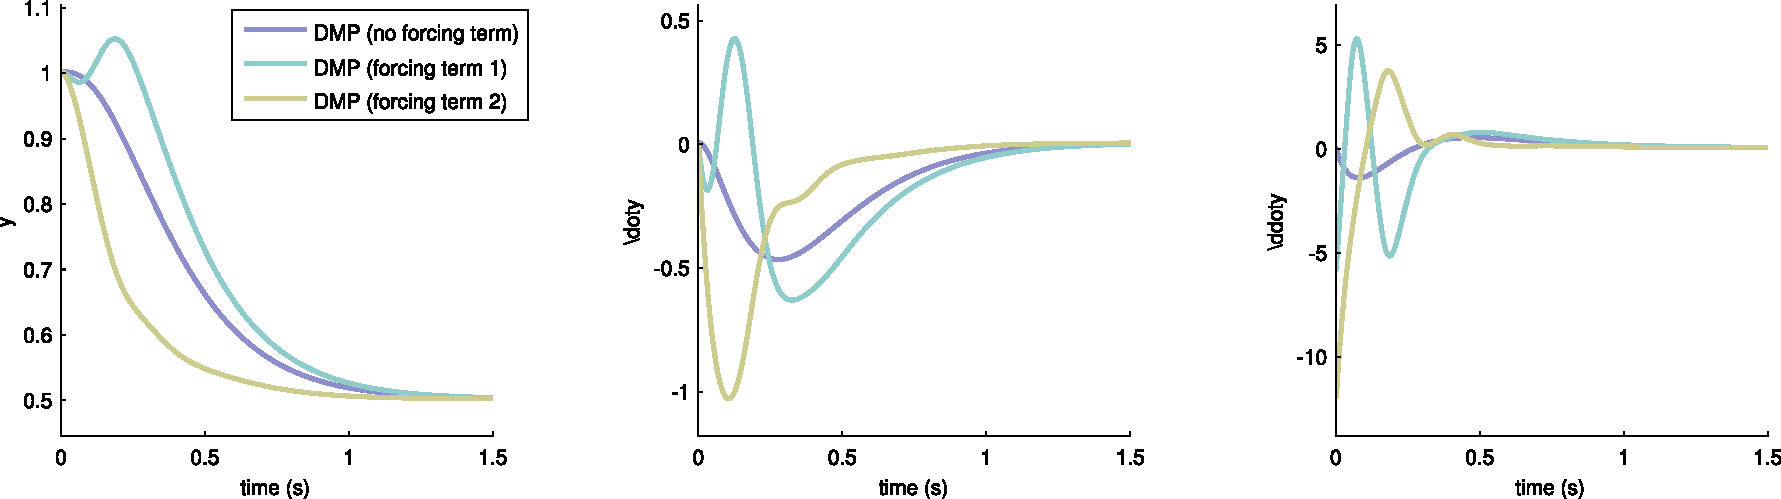
\includegraphics[height=4cm]{dmp_forcing_terms-svg}
\caption{A non-\/linear forcing term enable more complex trajectories to be generated (these D\+M\+Ps use a goal system and an exponential gating term).}
\end{DoxyImage}
\hypertarget{page_dmp_sec_forcing_convergence}{}\subsubsection{Ensuring Convergence to 0 of the Forcing Term\+: the Gating System}\label{page_dmp_sec_forcing_convergence}
Since we add a forcing term to the dynamical system, we can no longer guarantee that the system will converge towards $ x^g $; perhaps the forcing term continually pushes it away $ x^g $ (perhaps it doesn't, but the point is that we cannot {\itshape guarantee} that it {\itshape always} doesn't). That is why there is a question mark in the attractor state in the equation above. To guarantee that the movement will always converge towards the attractor $ x^g $, we need to ensure that the forcing term decreases to 0 towards the end of the movement. To do so, a gating term is added, which is 1 at the beginning of the movement, and 0 at the end. This gating term itself is determined by, of course, a dynamical system. In {\bfseries [ijspeert02movement]}, it was suggested to use an exponential system. We add this extra system to our dynamical system by expanding the state as follows\+:

\begin{eqnarray*} \dot{x} = \left[ \begin{array}{l} {\dot{z}} \\ {\dot{y}} \\ {\dot{x}} \end{array} \right] = \left[ \begin{array}{l} (\alpha_y (\beta_y({y}^{g}-{y})-{z}) + x\cdot f(t))/\tau \\ {z}/\tau \\ -\alpha_x x/\tau \end{array} \right] \mbox{~~~~with init. state~} \left[ \begin{array}{l} 0 \\ y_0 \\ 1 \end{array} \right] \mbox{~and attr. state~} \left[ \begin{array}{l} {0} \\ {y}^g \\ 0 \end{array} \right] \end{eqnarray*}\hypertarget{page_dmp_sec_forcing_autonomy}{}\subsubsection{Ensuring Autonomy of the Forcing Term\+: the Phase System}\label{page_dmp_sec_forcing_autonomy}
By introducing the dependence of the forcing term $ f(t)$ on time $ t $ the overall system is no longer autonomous. To achieve independence of time, we therefore let $ f $ be a function of the state of an (autonomous) dynamical system rather than of $ t $. This system represents the {\itshape phase} of the movement. {\bfseries [ijspeert02movement]} suggested to use the same dynamical system for the gating and phase, and use the term {\itshape canonical} {\itshape system} to refer this joint gating/phase system. Thus the phase of the movement starts at 1, and converges to 0 towards the end of the movement, just like the gating system. The new formulation now is (the only difference is $ f(x)$ instead of $ f(t)$)\+:

\begin{eqnarray*} \left[ \begin{array}{l} {\dot{z}} \\ {\dot{y}} \\ {\dot{x}} \end{array} \right] = \left[ \begin{array}{l} (\alpha_y (\beta_y({y}^{g}-{y})-{z}) + x\cdot f(x))/\tau \\ {z}/\tau \\ -\alpha_x x/\tau \end{array} \right] \mbox{~~~~with init. state~} \left[ \begin{array}{l} 0 \\ y_0 \\ 1 \end{array} \right] \mbox{~and attr. state~} \left[ \begin{array}{l} {0} \\ {y}^g \\ 0 \end{array} \right] \end{eqnarray*}

\begin{DoxyRefDesc}{Todo}
\item[\hyperlink{todo__todo000006}{Todo}]Discuss goal-\/dependent scaling, i.\+e. $ f(t)s(x^g-x_0) $?\end{DoxyRefDesc}
\hypertarget{page_dmp_sec_multidim_dmp}{}\subsubsection{Multi-\/dimensional Dynamic Movement Primitives}\label{page_dmp_sec_multidim_dmp}
Since D\+M\+Ps usually have multi-\/dimensional states (e.\+g. one output $ {\mathbf{y}}_{d=1\dots D}$ for each of the $ D $ joints), it is more accurate to use bold fonts for the state variables (except the gating/phase system, because it is always 1\+D) so that they represent vectors\+:

\begin{eqnarray*} \left[ \begin{array}{l} {\dot{\mathbf{z}}} \\ {\dot{\mathbf{y}}} \\ {\dot{x}} \end{array} \right] = \left[ \begin{array}{l} (\alpha_y (\beta_y({\mathbf{y}}^{g}-\mathbf{y})-\mathbf{z}) + x\cdot f(x))/\tau \\ \mathbf{z}/\tau \\ -\alpha_x x/\tau \end{array} \right] \mbox{~~~~with init. state~} \left[ \begin{array}{l} \mathbf{0} \\ \mathbf{z}_0 \\ 1 \end{array} \right] \mbox{~and attr. state~} \left[ \begin{array}{l} \mathbf{0} \\ \mathbf{y}^g \\ 0 \end{array} \right] \end{eqnarray*}

So far, the graphs have shown 1-\/dimensional systems. To generate D-\/dimensional trajectories for, for instance, the 7 joints of an arm or the 3\+D position of its end-\/effector, we simply use D transformation systems. A key principle in D\+M\+Ps is to use one and the same phase system for all of the transformation systems, to ensure that the output of the transformation systems are synchronized in time. The image below show the evolution of all the dynamical systems involved in integrating a multi-\/dimensional D\+M\+P.


\begin{DoxyImage}
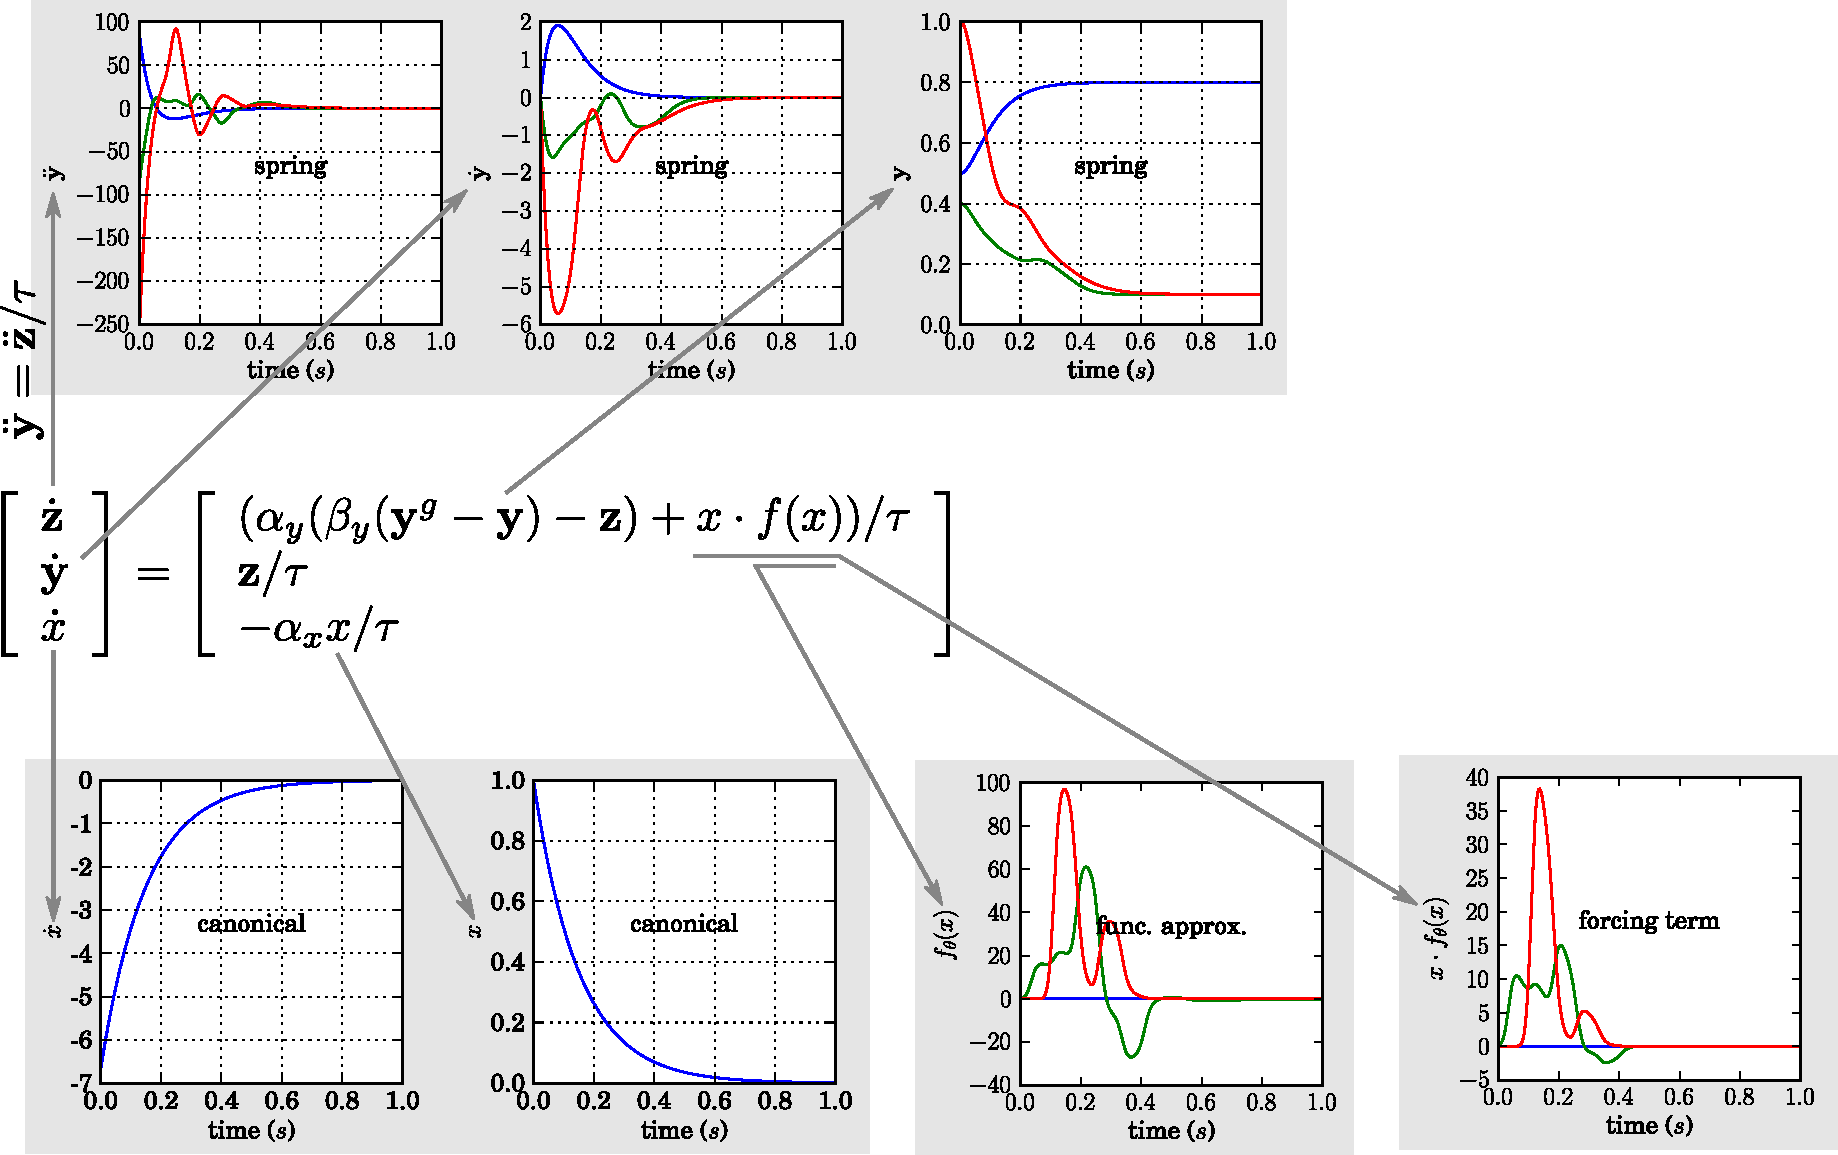
\includegraphics[height=8cm]{dmpplot_ijspeert2002movement-svg}
\caption{The various dynamical systems and forcing terms in multi-\/dimensional D\+M\+Ps.}
\end{DoxyImage}


{\itshape }

{\itshape }\hypertarget{page_dyn_sys_Implementation}{}\subsubsection{Implementation}\label{page_dyn_sys_Implementation}
{\itshape  Since a Dynamical Movement Primitive is a dynamical system, the Dmp class derives from the Dynamical\+System class. It overrides the virtual function Dynamical\+System\+::integrate\+Start(). Integrating the D\+M\+P numerically (Euler or 4th order Runge-\/\+Kutta) is done with the generic Dynamical\+System\+::integrate\+Step() function. It also implements the pure virtual function Dynamical\+System\+::analytical\+Solution(). Because a D\+M\+P cannot be solved analytically (we cannot write it in closed form due to the arbitrary forcing term), calling Dmp\+::analytical\+Solution() in fact performs a numerical Euler integration (although the linear subsystems (phase, gating, etc.) are analytically solved because this is faster computationally).}

{\itshape Please note that in this tutorial we have used the notation $[z~y]$ for consistency with the D\+M\+P literature. In the C++ implementation, the order is rather $[y~z]$.}

{\itshape {\itshape Remark}. Dmp inherits the function Dynamical\+System\+::integrate\+Step() from the Dynamical\+System class. Dynamical\+System\+::integrate\+Step() uses either Euler integration, or 4-\/th order Runge-\/\+Kutta. The latter is more accurate, but requires 4 calls of Dynamical\+System\+::differential\+Equation() instead of 1). Which one is used can be set with Dynamical\+System\+::set\+\_\+integration\+\_\+method(). To numerically integrate a dynamical system, one must carefully choose the integration time dt. Choosing it too low leads to inaccurate integration, and the numerical integration will diverge from the 'true' solution acquired through analytical solution. See \href{http://en.wikipedia.org/wiki/Euler%27s_method}{\tt http\+://en.\+wikipedia.\+org/wiki/\+Euler\%27s\+\_\+method} for examples. Choosing dt depends entirely on the time-\/scale (seconds vs. years) and parameters of the dynamical system (time constant, decay parameters). For D\+M\+Ps, which are expected to take between 0.\+5-\/10 seconds, dt is usually chosen to be in the range 0.\+01-\/0.\+001. }\hypertarget{page_dmp_sec_dmp_alternative}{}\subsection{Alternative Systems for Gating, Phase and Goals}\label{page_dmp_sec_dmp_alternative}
\hypertarget{page_dmp_sec_dmp_sigmoid_gating}{}\subsubsection{Gating\+: Sigmoid System}\label{page_dmp_sec_dmp_sigmoid_gating}
A disadvantage of using an exponential system as a gating term is that the gating decreases very quickly in the beginning. Thus, the output of the function approximator $ f(x) $ needs to be very high towards the end of the movement if it is to have any effect at all. This leads to scaling issues when training the function approximator.

Therefore, sigmoid systems have more recently been proposed {\bfseries [kulvicius12joining]} as a gating system. This leads to the following D\+M\+P formulation (since the gating and phase system are no longer shared, we introduce a new state variable $ v $ for the gating term\+:

\begin{eqnarray*} \left[ \begin{array}{l} {\dot{\mathbf{z}}} \\ {\dot{\mathbf{y}}} \\ {\dot{x}} \\ {\dot{v}} \end{array} \right] = \left[ \begin{array}{l} (\alpha_y (\beta_y({\mathbf{y}}^{g}-\mathbf{y})-\mathbf{z}) + v\cdot f(x))/\tau \\ \mathbf{z}/\tau \\ -\alpha_x x/\tau \\ -\alpha_v v (1-v/v_{\mbox{\scriptsize max}}) \end{array} \right] \mbox{~~~~with init. state~} \left[ \begin{array}{l} \mathbf{0} \\ \mathbf{y}_0 \\ 1 \\ 1 \end{array} \right] \mbox{~and attr. state~} \left[ \begin{array}{l} \mathbf{0} \\ \mathbf{y}^g \\ 0 \\ 0 \end{array} \right] \end{eqnarray*}

where the term $ v_{\mbox{\scriptsize max}}$ is determined by $\tau $\hypertarget{page_dmp_sec_dmp_phase}{}\subsubsection{Phase\+: Constant Velocity System}\label{page_dmp_sec_dmp_phase}
In practice, using an exponential phase system may complicate imitation learning of the function approximator $ f $, because samples are not equidistantly spaced in time. Therefore, we introduce a dynamical system that mimics the properties of the phase system described in {\bfseries [kulvicius12joining]}, whilst allowing for a more natural integration in the D\+M\+P formulation, and thus our code base. This system starts at 0, and has a constant velocity of $1/\tau$, which means the system reaches 1 when $t=\tau$. When this point is reached, the velocity is set to 0.

\begin{eqnarray*} \dot{x} =& 1/\tau \mbox{~if~} x < 1 & \\ & 0 \mbox{~if~} x>1 \\ \end{eqnarray*}

This, in all honesty, is a bit of a hack, because it leads to a non-\/smooth acceleration profile. However, its properties as an input to the function approximator are so advantageous that we have designed it in this way (the implementation of this system is in the Time\+System class).


\begin{DoxyImage}
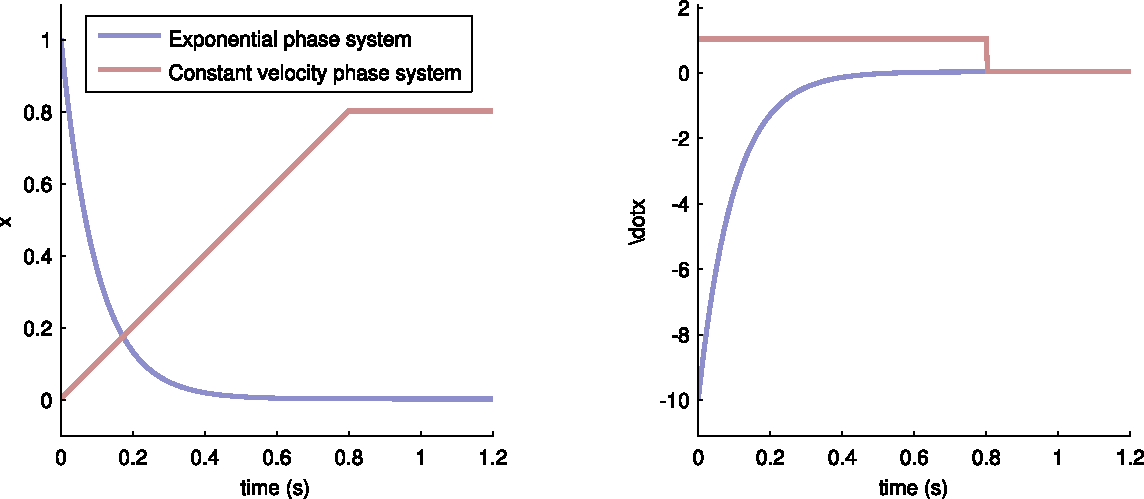
\includegraphics[height=4cm]{phase_systems-svg}
\caption{Exponential and constant velocity dynamical systems as the 1\+D phase for a dynamical movement primitive.}
\end{DoxyImage}


With the constant velocity dynamical system the D\+M\+P formulation becomes\+:

\begin{eqnarray*} \left[ \begin{array}{l} {\dot{\mathbf{z}}} \\ {\dot{\mathbf{y}}} \\ {\dot{x}} \\ {\dot{v}} \end{array} \right] = \left[ \begin{array}{l} (\alpha_y (\beta_y({\mathbf{y}}^{g}-\mathbf{y})-\mathbf{z}) + v\cdot f(x))/\tau \\ \mathbf{z}/\tau \\ 1/\tau \\ -\alpha_v v (1-v/v_{\mbox{\scriptsize max}}) \end{array} \right] \mbox{~~~~with init. state~} \left[ \begin{array}{l} \mathbf{0} \\ \mathbf{y}_0 \\ 0 \\ 1 \end{array} \right] \mbox{~and attr. state~} \left[ \begin{array}{l} \mathbf{0} \\ \mathbf{y}^g \\ 1 \\ 0 \end{array} \right] \end{eqnarray*}\hypertarget{page_dmp_sec_delayed_goal}{}\subsubsection{Zero Initial Accelerations\+: the Delayed Goal System}\label{page_dmp_sec_delayed_goal}
Since the spring-\/damper system leads to high initial accelerations (see the graph to the right below), which is usually not desirable for robots, it was suggested to move the attractor of the system from the initial state $ y_0 $ to the goal state $ y^g $ {\itshape during} the movement {\bfseries [kulvicius12joining.]} This delayed goal attractor $ y^{g_d} $ itself is represented as an exponential dynamical system that starts at $ y_0 $, and converges to $ y^g $ (in early versions of D\+M\+Ps, there was no delayed goal system, and $ y^{g_d} $ was simply equal to $ y^g $ throughout the movement). The combination of these two systems, listed below, leads to a movement that starts and ends with 0 velocities and accelerations, and approximately has a bell-\/shaped velocity profile. This representation is thus well suited to generating human-\/like point-\/to-\/point movements, which have similar properties.

\begin{eqnarray*} \left[ \begin{array}{l} {\dot{\mathbf{z}}} \\ {\dot{\mathbf{y}}} \\ {\dot{\mathbf{y}}^{g_d}} \\ {\dot{x}} \\ {\dot{v}} \end{array} \right] = \left[ \begin{array}{l} (\alpha_y (\beta_y({\mathbf{y}}^{g_d}-\mathbf{y})-\mathbf{z}) + v\cdot f(x))/\tau \\ \mathbf{z}/\tau \\ -\alpha_g({\mathbf{y}^g-\mathbf{y}^{g_d}}) \\ 1/\tau \\ -\alpha_v v (1-v/v_{\mbox{\scriptsize max}}) \end{array} \right] \mbox{~~~~with init. state~} \left[ \begin{array}{l} \mathbf{0} \\ \mathbf{y}_0 \\ \mathbf{y}_0 \\ 0 \\ 1 \end{array} \right] \mbox{~and attr. state~} \left[ \begin{array}{l} \mathbf{0} \\ \mathbf{y}^g \\ \mathbf{y}^g \\ 1 \\ 0 \end{array} \right] \end{eqnarray*}


\begin{DoxyImage}
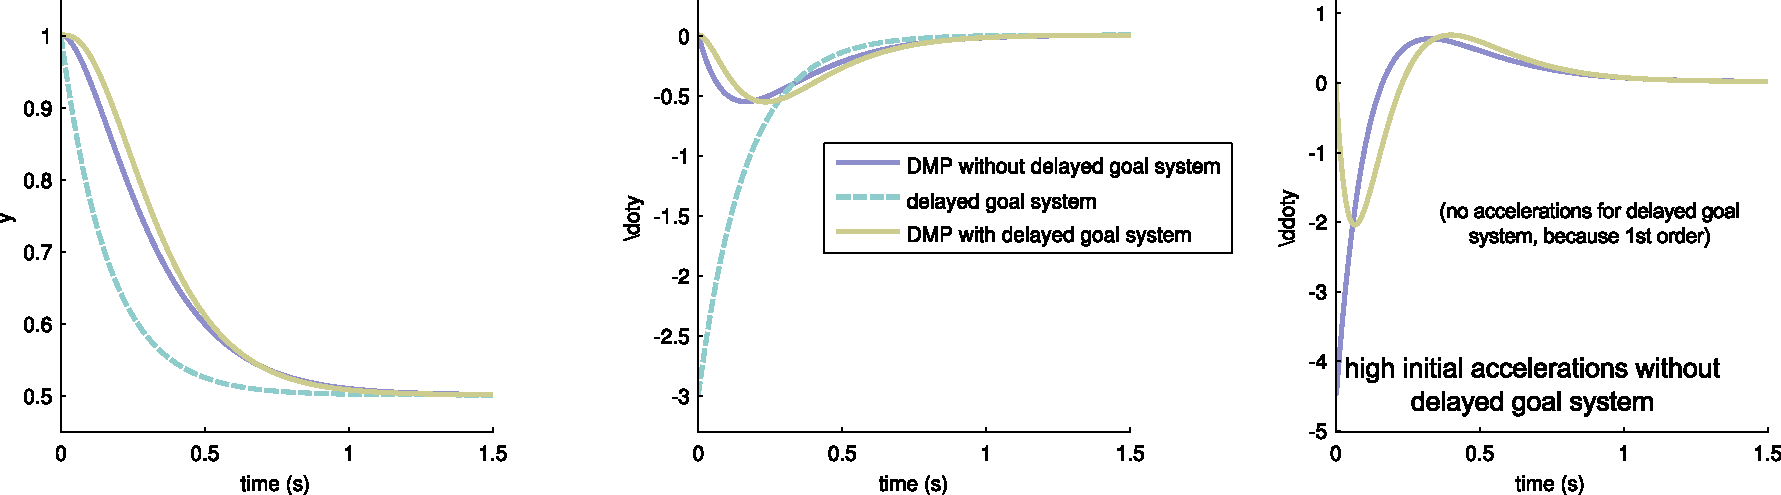
\includegraphics[height=4cm]{dmp_and_goal_system-svg}
\caption{A first dynamical movement primitive, with and without a delayed goal system (left\+: state variable, center\+: velocities, right\+: accelerations.}
\end{DoxyImage}


In my experience, this D\+M\+P formulation is the best for learning human-\/like point-\/to-\/point movements (bell-\/shaped velocity profile, approximately zero velocities and accelerations at beginning and start of the movement), and generates nice normalized data for the function approximator without scaling issues (an exact empirical evaluation is on the stack...). The image below shows the interactions between the spring-\/damper system, delayed goal system, phase system and gating system.


\begin{DoxyImage}
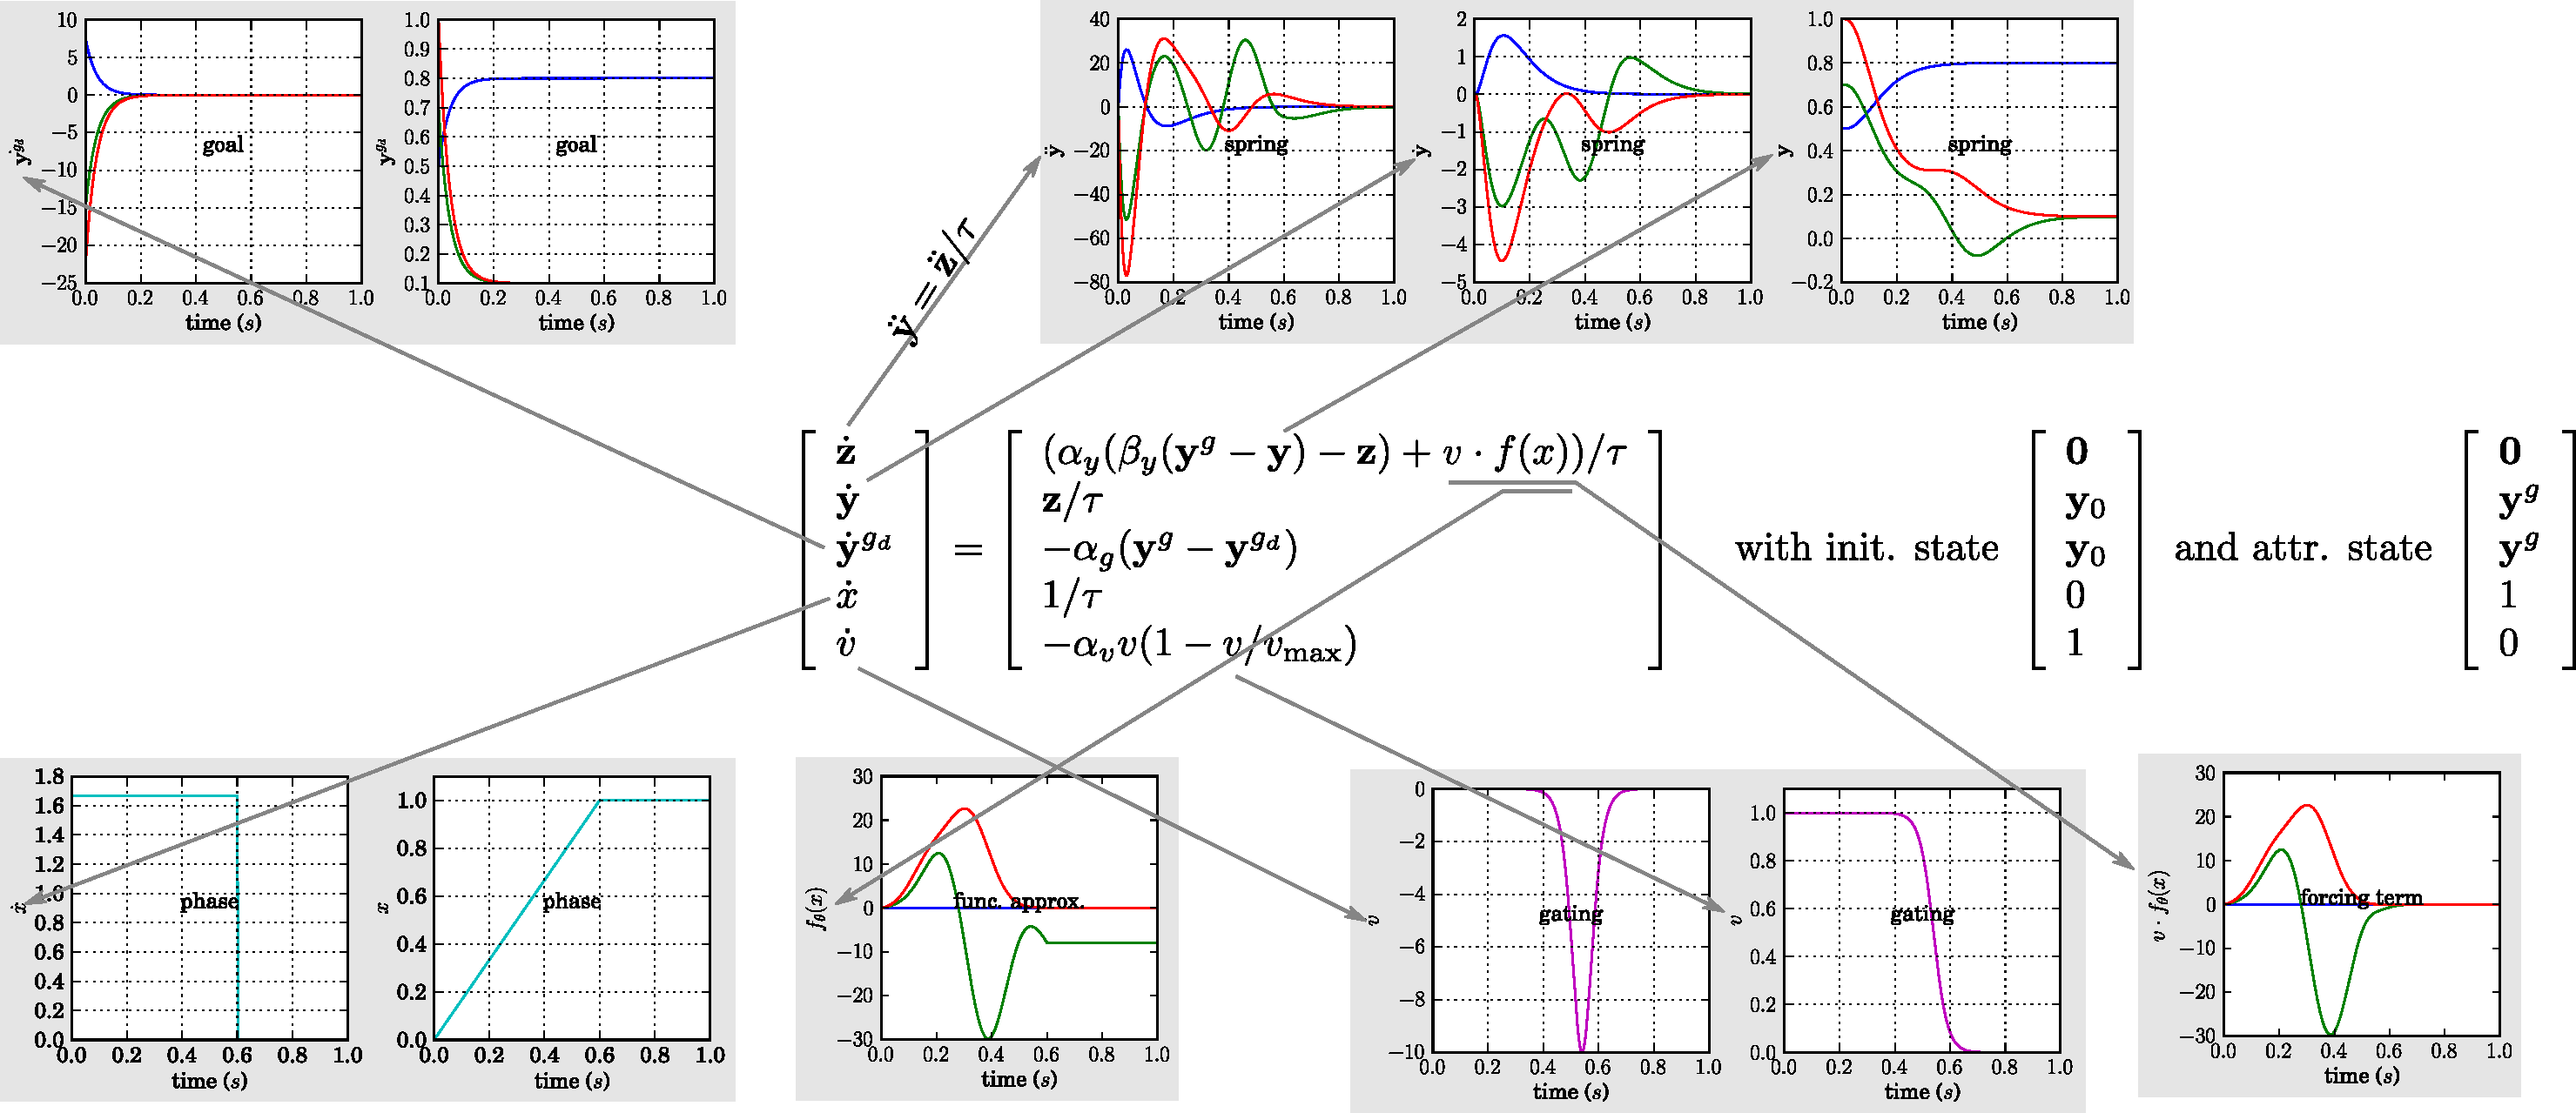
\includegraphics[height=7cm]{dmpplot_kulvicius2012joining-svg}
\caption{The various dynamical systems and forcing terms in multi-\/dimensional D\+M\+Ps.}
\end{DoxyImage}
\hypertarget{page_dmp_sec_dmp_issues}{}\subsection{Known Issues}\label{page_dmp_sec_dmp_issues}
\begin{DoxyRefDesc}{Todo}
\item[\hyperlink{todo__todo000007}{Todo}]Known Issues\end{DoxyRefDesc}


\begin{DoxyItemize}
\item Scaling towards novel goals\end{DoxyItemize}
\hypertarget{page_dmp_sec_dmp_summary}{}\subsection{Summary}\label{page_dmp_sec_dmp_summary}
The core idea in dynamical movement primitives is to combine dynamical systems, which have nice properties in terms of convergence towards the goal, robustness to perturbations, and independence of time, with function approximators, which allow for the generation of arbitrary (smooth) trajectories. The key enabler to this approach is to gate the output of the function approximator with a gating system, which is 1 at the beginning of the movement, and 0 towards the end.

Further enhancements can be made by making the system autonomous (by using the output of a phase system rather than time as an input to the function approximator), or having initial velocities and accelerations of 0 (by using a delayed goal system).

Multi-\/dimensional D\+M\+Ps are achieved by using multi-\/dimensional dynamical systems, and learning one function approximator for each dimension. Synchronization of the different dimensions is ensure by coupling them with only {\itshape one} phase system. 
\section{Black Box Optimization of Dynamical Movement Primitives}
\label{page_dmp_bbo}
\hypertarget{page_dmp_bbo}{}
\input{page_dmp_bbo}
\section{Serialization}
\label{page_serialization}
\hypertarget{page_serialization}{}
Serialization and deserialization of objects serves two purposes in this code\+:

\begin{DoxyItemize}
\item Reading parameter/experiment settings from a file. For instance, you could specify the Meta\+Parameters of a Function\+Approximator in a file, read that file in your program, and train a Function\+Approximator with those Meta\+Parameters. To try different Meta\+Parameters settings you only have to change the input file, without having to recompile. To be able to edit such parameter files, the files should be human readable. Ideally, it should be J\+S\+O\+N, because it is very readable and compact.\end{DoxyItemize}
\begin{DoxyItemize}
\item Saving the results of an experiment. Saving such results to binary files would be more compact, but to ensure that the same format is used for both serialization and deserialization, we use a human-\/readable format here also.\end{DoxyItemize}
I considered the following options.

\begin{DoxyItemize}
\item Boost property tree\+: it makes a mess of arrays when saving to J\+S\+O\+N\end{DoxyItemize}
\begin{DoxyItemize}
\item Google protobuf\+: I preferred to not have code generated for me\end{DoxyItemize}
\begin{DoxyItemize}
\item cereal\+: \href{http://uscilab.github.io/cereal/,}{\tt http\+://uscilab.\+github.\+io/cereal/,} external library. Really the best option, but I tried to avoid users having to use non-\/standard libraries.\end{DoxyItemize}
\begin{DoxyItemize}
\item jsoncpp\+: Not ideal for serialization, more for read/write of J\+S\+O\+N.\end{DoxyItemize}
In summary, I could not find any libraries that were easy to install and could serialize to/from J\+S\+O\+N. Therefore, I went for the second choice, which was X\+M\+L. Because boost is a standard, and compiles on most platforms, I decided to use boost\+:\+: serialization. I consider this to be quite a compromise, because I find boost\+::serialization quite messy, it is not well documented, and it took me quite a while to get it working properly (especially the registering of derived classes, for which you have to use a wierd combination of macros in the exact right places)

Since I was writing to X\+M\+L with boost\+::serialization anyway, many classes implement a to\+String() method that simply returns the X\+M\+L code (without a header) that results from serialization. The R\+E\+T\+U\+R\+N\+\_\+\+S\+T\+R\+I\+N\+G\+\_\+\+F\+R\+O\+M\+\_\+\+B\+O\+O\+S\+T\+\_\+\+S\+E\+R\+I\+A\+L\+I\+Z\+A\+T\+I\+O\+N\+\_\+\+X\+M\+L macro does all the work for writing to an X\+M\+L archive and converting it to a string. Having X\+M\+L as output is not ideal, but it avoid lots of duplicate code. Perhaps boost\+::serialization will one day be able to write to J\+S\+O\+N also, and then this could be used instead.

I decided to go for string to\+String(void) instead of ostream\& to\+Stream(ostream\&), because to\+String allows you to easily use both the output stream operator (output $<$$<$ obj.\+to\+String()) and printf (printf(\char`\"{}\%s\char`\"{},obj.\+to\+String()), whereas to\+Stream would be much more messy to use in combination with printf (not everyone likes to use the outputstream operator).\hypertarget{page_serialization_sec_boost_serialization_ugliness}{}\subsection{Boost serialization issues}\label{page_serialization_sec_boost_serialization_ugliness}
With boost\+::serialization, it is possible to serialize classes without a default constuctor with \href{http://www.boost.org/doc/libs/1_55_0/libs/serialization/doc/serialization.html#constructors}{\tt http\+://www.\+boost.\+org/doc/libs/1\+\_\+55\+\_\+0/libs/serialization/doc/serialization.\+html\#constructors} But load\+\_\+construct\+\_\+data requires the creation of an object, which we cannot when classes are abstract. It seems no-\/one knows how to solve this\+: \begin{DoxyItemize}
\item \href{http://lists.boost.org/boost-users/2005/09/13827.php}{\tt http\+://lists.\+boost.\+org/boost-\/users/2005/09/13827.\+php} \item \href{http://boost.2283326.n4.nabble.com/serialization-Serializing-classes-with-no-default-constructors-td2557921.html}{\tt http\+://boost.\+2283326.\+n4.\+nabble.\+com/serialization-\/\+Serializing-\/classes-\/with-\/no-\/default-\/constructors-\/td2557921.\+html}\end{DoxyItemize}
For this reason abstract base classes that are to be serialized with boost must have a default constructor, and may not have const members. This is really a pain, because a serialization library should not enforce such design decisions... But this is the way it is in the code.\hypertarget{page_serialization_sec_eigen_boost_serialization}{}\subsection{Serializing boost matrices}\label{page_serialization_sec_eigen_boost_serialization}
To avoid bloating the serialization of Eigen matrices with lots of X\+M\+L tags, they are serialized in a special way. The following examples show how Eigen matrices are serialized in X\+M\+L\+:

\begin{DoxyItemize}
\item Standard matrix\+: 
\begin{DoxyCode}
<m>2X3; 0 0 0; 1 1 1</m>
\end{DoxyCode}
\end{DoxyItemize}
\begin{DoxyItemize}
\item Vector\+: 
\begin{DoxyCode}
<m>3X1; 0 0 0</m>
<m>1X3; 0 0 0</m>
\end{DoxyCode}
\end{DoxyItemize}
\begin{DoxyItemize}
\item Diagonal matrix (only the diagonal is saved, indicated with D instead of X\+: 
\begin{DoxyCode}
<m>3D3; 1 2 3</m>
\end{DoxyCode}
 \end{DoxyItemize}

\section{Dynamical Systems Module}
\label{page_dyn_sys}
\hypertarget{page_dyn_sys}{}
\hypertarget{page_dyn_sys_sec_dyn_sys_intro}{}\subsection{Introduction}\label{page_dyn_sys_sec_dyn_sys_intro}
Let a {\itshape state} be a vector of real numbers. A dynamical system consists of such a state and a rule that describes how this state will change over time; it describes what future state follows from the current state. A typical example is radioactive decay, where the state $x$ is the number of atoms, and the rate of decay is $\frac{dx}{dt}$ proportional to $x$\+: $ \frac{dx}{dt} = -\alpha x$. Here, $\alpha$ is the `decay constant' and $\dot{x}$ is a shorthand for $\frac{dx}{dt}$. Such an evolution rule describes an implicit relation between the current state $ x(t) $ and the state a short time in the future $x(t+dt)$.

If we know the initial state of a dynamical system, e.\+g. $x_0\equiv x(0)=4$, we may compute the evolution of the state over time through {\itshape numerical} {\itshape integration}. This means we take the initial state $ x_0$, and iteratively compute subsequent states $x(t+dt)$ by computing the rate of change $\dot{x}$, and integrating this over the small time interval $dt$. A pseudo-\/code example is shown below for $x_0\equiv x(0)=4$, $dt=0.01s$ and $\alpha=6$.


\begin{DoxyCode}
alpha=6; \textcolor{comment}{// Decay constant}
dt=0.01; \textcolor{comment}{// Duration of one integration step}
x=4.0;   \textcolor{comment}{// Initial state}
t=0.0;   \textcolor{comment}{// Initial time}
\textcolor{keywordflow}{while} (t<1.5) \{
  dx = -alpha*x;  \textcolor{comment}{// Dynamical system rule}
  x = x + dx*dt;  \textcolor{comment}{// Project x into the future for a small time step dt (Euler integration)}
  t = t + dt;     \textcolor{comment}{// The future is now!}
\}
\end{DoxyCode}


This procedure is called ``integrating the system'', and leads the trajectory plotted below (shown for both $\alpha=6$ and $\alpha=3$.


\begin{DoxyImage}
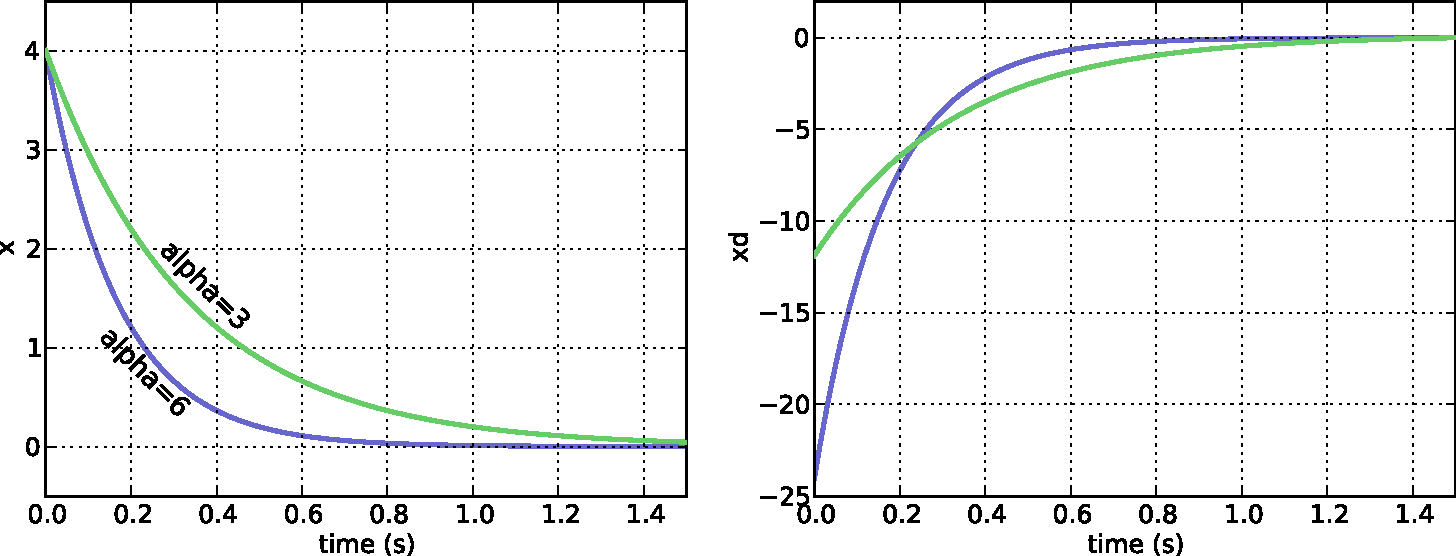
\includegraphics[height=4cm]{exponential_decay-svg}
\caption{Evolution of the exponential dynamical system.}
\end{DoxyImage}


The evolution of many dynamical systems can also be determined analytically, by explicitly solving the differential equation. For instance, $N(t) = x_0e^{-\alpha t}$ is the solution to $\dot{x} = -\alpha x$. Why? Let's plug $x(t) = x_0e^{-\alpha t}$ into $\frac{dx}{dt} = -\alpha x$, which leads to $\frac{d}{dt}(x_0e^{-\alpha t}) = -\alpha (x_0e^{-\alpha t})$. Then derive the left side of the equations, which yields $-\alpha(x_0e^{-\alpha t}) = -\alpha (x_0e^{-\alpha t})$. Q\+E\+D. Note that the solution works for arbitrary $x_0$. It should, because the solution should not depend on the initial state.\hypertarget{page_dyn_sys_dynsys_implementation1}{}\subsubsection{Implementation}\label{page_dyn_sys_dynsys_implementation1}
{\itshape  In the object-\/oriented implementation of this module, all dynamical systems inherit from the abstract Dynamical\+System class. The analytical solution of a dynamical system is computed with Dynamical\+System\+::analytical\+Solution, which takes the times {\ttfamily ts} at which the solution should be computed, and returns the evolution of the system as {\ttfamily xs} and {\ttfamily xds}.}

{\itshape A system's differential equation is implement in the function Dynamical\+System\+::differential\+Equation, which takes the current state {\ttfamily x}, and computes the rates of change {\ttfamily xd}. The functions Dynamical\+System\+::integrate\+Start() and Dynamical\+System\+::integrate\+Step() are then used to numerically integrate the system as follows (using the example plotted above)\+:}

{\itshape 
\begin{DoxyCode}
\textcolor{comment}{// Make exponential system that decays from 4 to 0 with decay constant 6, and tau=1.0}
\textcolor{keywordtype}{double} alpha = 6.0;                \textcolor{comment}{// Decay constant}
\textcolor{keywordtype}{double} tau = 1.0;                  \textcolor{comment}{// Time constant }
VectorXd x\_init(1); x\_init << 4.0; \textcolor{comment}{// Initial state (a 1D vector with the value 4.0 inside using Eigen
       comma initializer)}
VectorXd x\_attr(1); x\_attr << 0.0; \textcolor{comment}{// Attractor state}
DynamicalSystem* dyn\_sys = \textcolor{keyword}{new} ExponentialSystem(tau, x\_init, x\_attr, alpha);

Eigen::VectorXd x, xd;
dyn\_sys->integrateStart(x,xd); \textcolor{comment}{// Start the integration}
\textcolor{keywordtype}{double} dt = 0.01;
\textcolor{keywordflow}{for} (\textcolor{keywordtype}{double} t=0.0; t<1.5; t+=dt)
\{
  dyn\_sys->integrateStep(dt,x,x,xd);          \textcolor{comment}{// Takes current state x, integrates system, and writes next
       state in x, xd}
  cout << t << \textcolor{stringliteral}{" "} << x << \textcolor{stringliteral}{" "} << xd << endl; \textcolor{comment}{// Output current time, state and rate of change}
\}
\textcolor{keyword}{delete} dyn\_sys;
\end{DoxyCode}
}

{\itshape {\itshape Remark}. Both analytical\+Solution and differential\+Equation functions above are const, i.\+e. they do not change the Dynamical\+System itself.}

{\itshape {\itshape Remark}. Dynamical\+System\+::integrate\+Step uses either Euler integration, or 4-\/th order Runge-\/\+Kutta. The latter is more accurate, but requires 4 calls of Dynamical\+System\+::differential\+Equation() instead of 1). Which one is used can be set with Dynamical\+System\+::set\+\_\+integration\+\_\+method(). To numerically integrate a dynamical system, one must carefully choose the integration time dt. Choosing it too low leads to inaccurate integration, and the numerical integration will diverge from the 'true' solution acquired through analytical solution. See \href{http://en.wikipedia.org/wiki/Euler%27s_method}{\tt http\+://en.\+wikipedia.\+org/wiki/\+Euler\%27s\+\_\+method} for examples. Choosing dt depends entirely on the time-\/scale (seconds vs. years) and parameters of the dynamical system (time constant, decay parameters).}

{\itshape }\hypertarget{page_dyn_sys_dynsys_implementation1_plotting}{}\subsubsection{Plotting}\label{page_dyn_sys_dynsys_implementation1_plotting}
{\itshape  If you save the output of a dynamical in a file with format (where D is the dimensionality of the system, and T is the number of time steps) \begin{DoxyVerb}x^0_0 x^1_0 .. x^D_0   xd^0_0 xd^1_0 .. xd^D_0   t_0   
x^0_1 x^1_1 .. x^D_1   xd^0_1 xd^1_1 .. xd^D_1   t_1   
   :     :       :         :      :       :       :    
x^0_T x^1_T .. x^D_T   xd^0_T xd^1_T .. xd^D_T   t_T   
\end{DoxyVerb}
 you can plot this output with 
\begin{DoxyCode}
python dynamicalsystems/plotting/plotDynamicalSystem.py file.txt
\end{DoxyCode}
}

{\itshape }\hypertarget{page_dyn_sys_dynsys_implementation1_demo}{}\subsubsection{Demos}\label{page_dyn_sys_dynsys_implementation1_demo}
{\itshape  A demonstration of how to initialize and integrate an Exponential\+System is in \hyperlink{demoExponentialSystem_8cpp}{demo\+Exponential\+System.\+cpp}}

{\itshape A more complete demonstration including all implemented dynamical systems is in \hyperlink{demoDynamicalSystems_8cpp}{demo\+Dynamical\+Systems.\+cpp}. If you call the resulting executable with a directory argument, e.\+g. 
\begin{DoxyCode}
./demoDynamicalSystems /tmp/demoDynamicalSystems
\end{DoxyCode}
 it will save results to file, which you can plot with for instance\+: 
\begin{DoxyCode}
python plotDynamicalSystem.py /tmp/demoDynamicalSystems/ExponentialSystem/results\_rungekutta.txt
python plotDynamicalSystem.py /tmp/demoDynamicalSystems/ExponentialSystem/results\_euler.txt
\end{DoxyCode}
 Different test can be performed with the dynamical system. The test can be chosen by passing further argument, e.\+g. 
\begin{DoxyCode}
./demoDynamicalSystems /tmp/demoDynamicalSystems rungekutta euler
\end{DoxyCode}
 will integrate the dynamical systems with both the Runge-\/\+Kutta and simple Euler method. The available tests are\+: \begin{DoxyItemize}
\item \char`\"{}rungekutta\char`\"{} -\/ Use 4th-\/order Runge-\/\+Kutta integration (more accurate, but more calls of Dynamical\+System\+::differential\+Equation) \item \char`\"{}euler\char`\"{} -\/ Use simple Euler integration (less accurate, but faster) \item \char`\"{}analytical\char`\"{} -\/ Use the analytical solution instead of numerical integration \item \char`\"{}tau\char`\"{} -\/ Change tau before doing numerical integration \item \char`\"{}attractor\char`\"{} -\/ Change the attractor state during numerical integration \item \char`\"{}perturb\char`\"{} -\/ Perturb the state during numerical integration\end{DoxyItemize}
To compare for instance the analytical solution with the Runge-\/\+Kutta integration in a plot, you can do 
\begin{DoxyCode}
python plotDynamicalSystemComparison.py /tmp/demoDynamicalSystems/ExponentialSystem/results\_analytical.txt 
       /tmp/demoDynamicalSystems/ExponentialSystem/results\_rungekutta.txt
\end{DoxyCode}
}

{\itshape }\hypertarget{page_dyn_sys_sec_dyn_sys_properties}{}\subsection{Properties and Features of Linear Dynamical Systems}\label{page_dyn_sys_sec_dyn_sys_properties}
\hypertarget{page_dyn_sys_sec_dyn_sys_convergence}{}\subsubsection{Convergence towards the Attractor}\label{page_dyn_sys_sec_dyn_sys_convergence}
In the limit of time, the dynamical system for exponential decay will converge to 0 (i.\+e. $x(\infty) = x_0e^{-\alpha\infty} = 0$). The value 0 is known as the {\itshape attractor} of the system. For simple dynamical systems, it is possible to {\itshape proove} that they will converge towards the attractor.

Suppose that the attractor state in our running example is not 0, but 1. In that case, we change the attractor state of the exponential decay to $x^g$ ( $g$=goal) and define the following differential equation\+: \begin{eqnarray*} \dot{x} =& -\alpha(x-x^g) & \mbox{~with attractor } x^g \end{eqnarray*}

This system will now converge to the attractor state $x^g$, rather than 0.


\begin{DoxyImage}
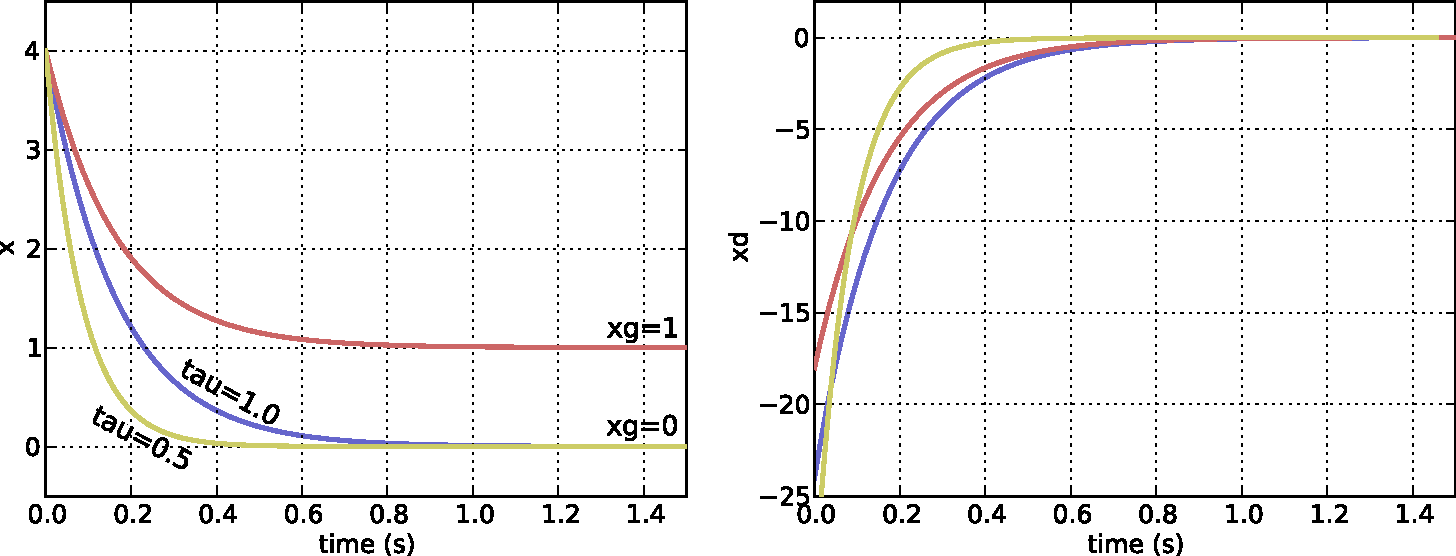
\includegraphics[height=4cm]{change_tau_attr-svg}
\caption{Changing the attractor state or time constant.}
\end{DoxyImage}
\hypertarget{page_dyn_sys_sec_dyn_sys_perturbations}{}\subsubsection{Robustness to Perturbations}\label{page_dyn_sys_sec_dyn_sys_perturbations}
Another nice feature of dynamical systems is their robustness to perturbations, which means that they will converge towards the attractor even if they are perturbed. The figure below shows how the perturbed system (cyan) converges towards the attractor state just as the unperturbed system (blue) does.


\begin{DoxyImage}
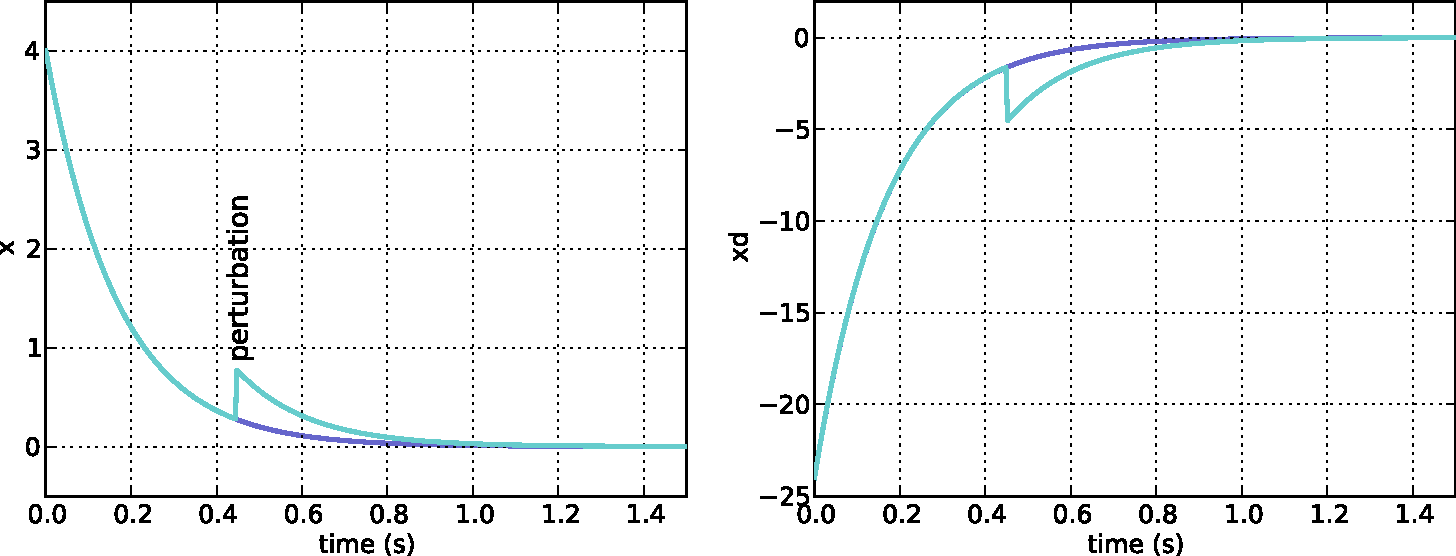
\includegraphics[height=4cm]{perturb-svg}
\caption{Perturbing the dynamical system.}
\end{DoxyImage}
\hypertarget{page_dyn_sys_sec_dyn_sys_time_constant}{}\subsubsection{Changing the speed of convergence\+: The time constant}\label{page_dyn_sys_sec_dyn_sys_time_constant}
The rates of change computed by the differential equation can be increased or decreased (leading to a faster or slower convergence) with a {\itshape time} {\itshape constant}, which is usually written as follows\+:

\begin{eqnarray*} \tau\dot{x} =& -\alpha(x-x^g)\\ \dot{x} =& (-\alpha(x-x^g))/\tau \end{eqnarray*}

{\itshape Remark}. For an exponential system, decreasing the time constant $\tau$ has the same effect as increasing $\alpha$. For more complex dynamical systems with several parameters, it is useful to have a separate parameter that changes only the speed of convergence, whilst leaving the other parameters the same.\hypertarget{page_dyn_sys_sec_dyn_sys_multi}{}\subsubsection{Multi-\/dimensional states}\label{page_dyn_sys_sec_dyn_sys_multi}
The state $x$ need not be a scalar, but may be a vector. This then represents a multi-\/dimensional state, i.\+e. $\tau\dot{\mathbf{x}} = -\alpha(\mathbf{x}-\mathbf{x}^g)$. In the code, the size of the state vector $dim(\mathbf{x})\equiv dim(\dot{\mathbf{x}})$ of a dynamical system is returned by the function Dynamical\+System\+::dim()\hypertarget{page_dyn_sys_sec_dyn_sys_autonomy}{}\subsubsection{Autonomy}\label{page_dyn_sys_sec_dyn_sys_autonomy}
Dynamical system that do not depend on time are called {\itshape autonomous}. For instance, the formula $ \dot{x} = -\alpha x$ does not depend on time, which means the exponential system is autonomous.\hypertarget{page_dyn_sys_Implementation}{}\subsubsection{Implementation}\label{page_dyn_sys_Implementation}
{\itshape  The attractor state and time constant of a dynamical system are usually passed to the constructor. They can be changed afterwards with with Dynamical\+System\+::set\+\_\+attractor\+\_\+state and Dynamical\+System\+::set\+\_\+tau. Before integration starts, the initial state can be set with Dynamical\+System\+::set\+\_\+initial\+\_\+state. This influences the output of Dynamical\+System\+::integrate\+Start, but not Dynamical\+System\+::integrate\+Step.}

{\itshape Further (first order) linear dynamical systems that are implemented in this module is a Sigmoid\+System (see \href{http://en.wikipedia.org/wiki/Exponential_decay}{\tt http\+://en.\+wikipedia.\+org/wiki/\+Exponential\+\_\+decay} and \href{http://en.wikipedia.org/wiki/Sigmoid_function}{\tt http\+://en.\+wikipedia.\+org/wiki/\+Sigmoid\+\_\+function}), as well as a dynamical system that has a constant velocity (Time\+System), so as to mimic the passing of time (time moves at a constant rate per time ;-\/)}

{\itshape  \begin{eqnarray*} \dot{x} =& -\alpha (x-x^g) & \mbox{exponential decay/growth} \label{equ_}\\ \dot{x} =& \alpha x (\beta-x) & \mbox{sigmoid} \label{equ_}\\ \dot{x} =& 1/\tau & \mbox{constant velocity (mimics the passage of time)} \label{equ_}\\ \end{eqnarray*}}

{\itshape 
\begin{DoxyImage}
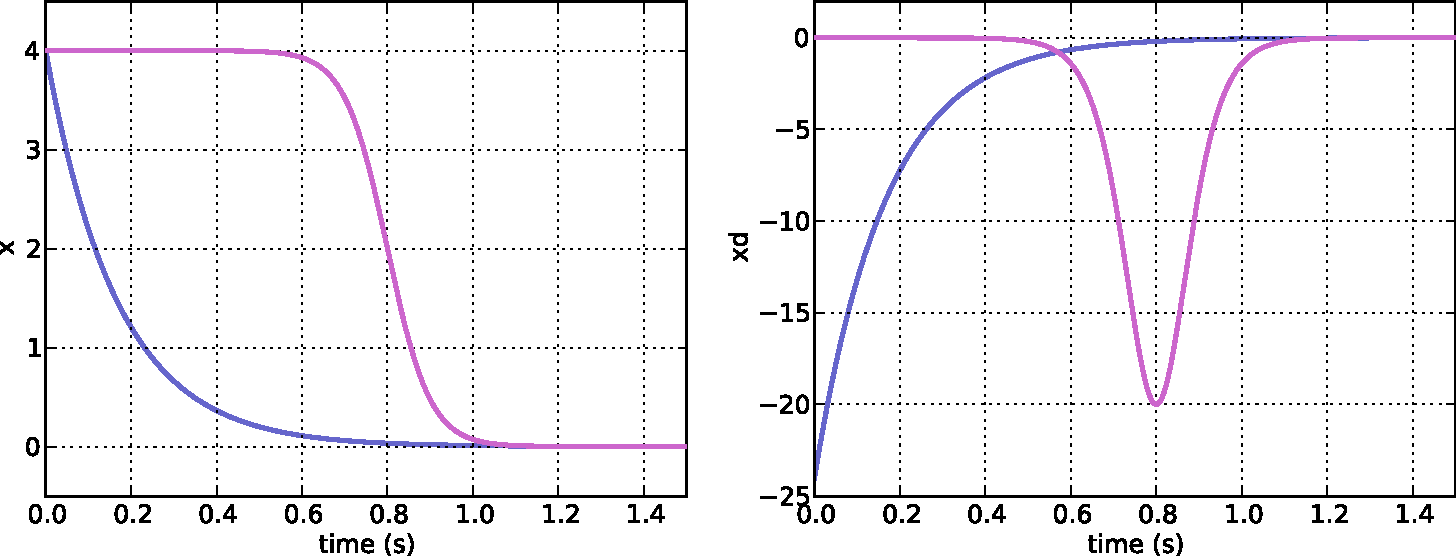
\includegraphics[height=4cm]{sigmoid-svg}
\caption{Exponential (blue) and sigmoid (purple) dynamical systems.}
\end{DoxyImage}
}

{\itshape }\hypertarget{page_dyn_sys_dyn_sys_second_order_systems}{}\subsection{Second-\/\+Order Systems}\label{page_dyn_sys_dyn_sys_second_order_systems}
The {\bfseries order} of a dynamical system is the order of the highest derivative in the differential equation. For instance, $\dot{x} = -\alpha x$ is of order 1, because the derivative with the highest order ( $\dot{x}$) has order 1. Such a system is known as a first-\/order system. All systems considered so far have been first-\/order systems, because the derivative with the highest order, i.\+e. $ \dot{x} $, has always been of order 1.\hypertarget{page_dyn_sys_dyn_sys_spring_damper}{}\subsubsection{Spring-\/\+Damper Systems}\label{page_dyn_sys_dyn_sys_spring_damper}
An example of a second order system (which also has terms $ \ddot{x} $) is a spring-\/damper system (see \href{http://en.wikipedia.org/wiki/Damped_spring-mass_system}{\tt http\+://en.\+wikipedia.\+org/wiki/\+Damped\+\_\+spring-\/mass\+\_\+system}), where $k$ is the spring constant, $c$ is the damping coefficient, and $m$ is the mass\+:

\begin{eqnarray*} m\ddot{x}=& -kx -c\dot{x} & \mbox{spring-damper (2nd order system)} \label{equ_}\\ \ddot{x}=& (-kx -c\dot{x})/m & \end{eqnarray*}\hypertarget{page_dyn_sys_dyn_sys_critical_damping}{}\subsubsection{Critical Damping}\label{page_dyn_sys_dyn_sys_critical_damping}
A spring-\/damper system is called critically damped when it converges to the attractor as quickly as possible without overshooting, as the red plot in \href{http://en.wikipedia.org/wiki/File:Damping_1.svg}{\tt http\+://en.\+wikipedia.\+org/wiki/\+File\+:\+Damping\+\_\+1.\+svg}. This happens when $c = 2\sqrt{mk}$.\hypertarget{page_dyn_sys_dyn_sys_rewrite_second_first}{}\subsubsection{Rewriting one 2nd Order Systems as two 1st Order Systems}\label{page_dyn_sys_dyn_sys_rewrite_second_first}
For implementation purposes, it is more convenient to work only with 1st order systems. Fortunately, we can expand the state $ x $ into two components $ x = [y~z]^T$ with $ z = \dot{y}$, and rewrite the differential equation as follows\+:

$ \left[ \begin{array}{l} \dot{y} \\ \dot{z} \end{array} \right] = \left[ \begin{array}{l} z \\ (-ky -cz)/m \end{array} \right] $

With this rewrite, the left term contains only first order derivatives, and the right term does not contain any derivatives. This is thus a first order system. Integrating such an expanded system is done just as one would integrate a dynamical system with a multi-\/dimensional state\+:\hypertarget{page_dyn_sys_Implementation}{}\subsubsection{Implementation}\label{page_dyn_sys_Implementation}
{\itshape  The constructor Dynamical\+System\+::\+Dynamical\+System immediately converts second order systems into first order systems with an expanded state.}

{\itshape The function Dynamical\+System\+::dim() returns the size of the entire state vector $ x = [y~z]$, the function Dynamical\+System\+::dim\+\_\+orig() return the size of only the $ y $ component. The attractor and initial state must always have the size returned by Dynamical\+System\+::dim\+\_\+orig(). } 
\section{Function Approximation Module}
\label{page_func_approx}
\hypertarget{page_func_approx}{}
\hypertarget{page_func_approx_sec_fa}{}\subsection{Function Approximation}\label{page_func_approx_sec_fa}
This module implements a set of function approximators, i.\+e. supervised learning algorithms that are trained with demonstration pairs input/target, after which they make predictions for new inputs. For simplicity, this module implements only batch learning (not incremental), and does not allow trained function approximators to be retrained.

The two main functions are Function\+Approximator\+::train, which takes a set of inputs and corresponding targets, and Function\+Approximator\+::predict, which makes predictions for novel inputs.\hypertarget{page_func_approx_sec_fa_metaparameters}{}\subsubsection{Meta\+Parameters and Model\+Parameters}\label{page_func_approx_sec_fa_metaparameters}
In this module, algorithmic parameters are called Meta\+Parameters, and the parameters of the model when the function approximator has been trained are called Model\+Parameters. The rationale for this is that an untrained function approximator can be entirely reconstructed if its Meta\+Parameters are known; this is useful for saving to file and making copies. A trained function approximator can be compeletely reconstructed given only its Model\+Parameters.

The life-\/cycle of a function approximator is as follows\+:

{\bfseries 1}. {\bfseries Initialization\+:} The function approximator is initialized by calling the constructor with the Meta\+Parameters. Its Model\+Parameters are set to N\+U\+L\+L, indicating that the model is untrained.

{\bfseries 2}. {\bfseries Training\+:} Function\+Approximator\+::train is called, which performs the conversion\+: $ \mbox{train}: \mbox{MetaParameters} \times \mbox{Inputs} \times \mbox{Targets} \mapsto \mbox{ModelParameters} $

{\bfseries 3}. {\bfseries Prediction\+:} Function\+Approximator\+::predict is called, which performs the conversion\+: $ \mbox{predict}: \mbox{ModelParameters} \times \mbox{Input} \mapsto \mbox{Output}$

{\itshape Remark}. Function\+Approximator\+::train in Step {\bfseries 2}. may only be called once. If you explicitly want to retrain the function approximator with novel input/target data call Function\+Approximator\+::re\+Train() instead.

{\itshape Remark}. During the initialization, Model\+Parameters may also be passed to the constructor. This means that an already trained function approximator is initialized. Step {\bfseries 2}. above is thus skipped.\hypertarget{page_func_approx_sec_fa_changing_modelparameters}{}\subsubsection{Changing the Model\+Parameters of a Function\+Approximator}\label{page_func_approx_sec_fa_changing_modelparameters}
The user should not be allowed to set the Model\+Parameters of a trained function approximator directly. Hence, Function\+Approximator\+::set\+Model\+Parameters is protected. However, in order to change the values inside the model parameters (for instance when optimizing them), the user may call Model\+Parameters\+::get\+Parameter\+Vector\+Selected and Model\+Parameters\+::set\+Parameter\+Vector\+Selected it inherits these functions from Parameterizable). These take a vector of doubles, check if the vector has the right size, and get/set the Model\+Parameters accordingly.

Function approximators often have different types of model parameters. For instance, the model parameters of Locally Weighted Regression (Function\+Approximator\+L\+W\+R) represent the centers and widths of the basis functions, as well as the slopes of the line segments. If you only want to get/set the slopes when calling Model\+Parameters\+::get\+Parameter\+Vector\+Selected and Model\+Parameters\+::set\+Parameter\+Vector\+Selected, you must use Model\+Parameters\+::set\+Selected\+Parameters(const std\+::set$<$std\+::string$>$\& selected\+\_\+values\+\_\+labels), for instance as follows\+:


\begin{DoxyCode}
std::set<std::string> selected;
selected.insert(\textcolor{stringliteral}{"slopes"});
model\_parameters.setSelectedParameters(selected);
Eigen::VectorXd values;
model\_parameters.getParameterVectorSelected(values);
\textcolor{comment}{// "values" now only contains the slopes of the line segments}

selected.clear();
selected.insert(\textcolor{stringliteral}{"centers"});
selected.insert(\textcolor{stringliteral}{"slopes"});
model\_parameters.setSelectedParameters(selected);
model\_parameters.getParameterVectorSelected(values);
\textcolor{comment}{// "values" now contains the centers of the basis functions AND slopes of the line segments}
\end{DoxyCode}


The rationale behind this implementation is that optimizers (such as evolution strategies) should not have to care about whether a particular set of model parameters contains centers, widths or slopes. Therefore, these different types of parameters are provided in one vector without semantics, and the generic interface is provided by the Parameterizable class.

Classes that inherit from Parameterizable (such as all Model\+Parameters and Function\+Approximator subclasses, must implement the pure virtual methods Parameterizable\+::get\+Parameter\+Vector\+All Parameterizable\+::set\+Parameter\+Vector\+All and Parameterizable\+::get\+Parameter\+Vector\+Mask. Which gets/sets all the possible parameters in one vector, and a mask specifying the semantics of each value in the vector. The work of setting/getting the selected parameters (and normalizing them) is done in the Parameterizable class itself. This approach is a slightly longer run-\/time than doing the work in the subclasses, but it leads to more legible and robust code (less code duplication).\hypertarget{page_func_approx_sec_caching_basisfunctions}{}\subsubsection{Caching of basis functions}\label{page_func_approx_sec_caching_basisfunctions}
If the parameters of the basis functions (centers and widths of the kernels) do not change often, you can cache the basis function activations by calling Model\+Parameters\+::set\+\_\+caching(true). This can lead to speed improvements because the activations are not computed over and over again. This function only makes senses if the inputs remain the same, i.\+e. this is not the case when running on a real robot.

The reason why caching is implemented in Model\+Parameters, and not in Function\+Approximator is because Model\+Parameters knows which parts of the Model\+Parameters change the basis function activations, and which do not (for instance in R\+B\+F\+N, the widths and centers change the basis function activations, but the weights do not). 
\section{Unified Model}
\label{page_unified_model}
\hypertarget{page_unified_model}{}
Whilst coding this library and numerous discussion with Olivier Sigaud, it became apparent that the latent function representations of all the function approximators in this library all use the same generic model.

Each specific model (i.\+e. as used in G\+P\+R, G\+M\+R, L\+W\+R, etc.) is a special case of the Unified Model. We discuss this in a forthcoming paper titled\+: \char`\"{}\+Many Regression Algorithms, One Unified Model -\/ A Review, Freek Stulp and Olivier Sigaud\char`\"{}, which you should be able to find in an on-\/line search. 
\section{Design Rationale}
\label{page_design}
\hypertarget{page_design}{}
\hypertarget{page_design_sec_remarks}{}\subsection{General Remarks}\label{page_design_sec_remarks}
\begin{DoxyItemize}
\item Code legibility is more important to me than absolute execution speed (except for those parts of the code likely to be called in a time-\/critical context) or using all of the design patterns known to man (that is why I do not use P\+I\+M\+P\+L; it is not so legible for the uninitiated user. Also, I do not use the factory design pattern, but rather have clone() functions in classes ).\end{DoxyItemize}
\begin{DoxyItemize}
\item I learned to use Eigen whilst coding this project (learning-\/by-\/doing). So especially the parts I coded first might have some convoluted solutions (I didn't learn about Eigen\+::\+Ref til later...). Any suggestions for making the code more legible or efficient are welcome. The same goes for Python actually. So be gentle on me on this one; I myself will probably look back at this Python code in a few years and think\+: \char`\"{}\+How cute... I was just a Python baby when I coded that.\char`\"{}\end{DoxyItemize}
\begin{DoxyItemize}
\item For the organization of the code (directory structure), I went with this suggestion\+: \href{http://stackoverflow.com/questions/13521618/c-project-organisation-with-gtest-cmake-and-doxygen/13522826#13522826}{\tt http\+://stackoverflow.\+com/questions/13521618/c-\/project-\/organisation-\/with-\/gtest-\/cmake-\/and-\/doxygen/13522826\#13522826}\end{DoxyItemize}
\begin{DoxyItemize}
\item In function signatures, inputs come first (if they are references, they are const) and then outputs (if they are not const, they are inputs for sure). Exception\+: if input arguments have default values, they can come after outputs. Virtual functions should not have default function arguments (this is confusing in the derived classes). If they really need them, then you have to make different functions with different argument lists (see for example Dmp\+Contextual\+::train(), there are 6 of them for this reason).\end{DoxyItemize}
\hypertarget{page_design_sec_naming}{}\subsection{Naming convention}\label{page_design_sec_naming}
I mainly follow the following naming style\+: \href{http://google-styleguide.googlecode.com/svn/trunk/cppguide.xml#Naming}{\tt http\+://google-\/styleguide.\+googlecode.\+com/svn/trunk/cppguide.\+xml\#\+Naming}

Notes\+: \begin{DoxyItemize}
\item Members end with a \+\_\+, i.\+e. {\ttfamily this\+\_\+is\+\_\+a\+\_\+member\+\_\+}. (Exception\+: members in a P\+O\+D (plain old data) class, which are public, and can be accessed directly) \item I also use this convention\+: \href{http://google-styleguide.googlecode.com/svn/trunk/cppguide.xml#Access_Control}{\tt http\+://google-\/styleguide.\+googlecode.\+com/svn/trunk/cppguide.\+xml\#\+Access\+\_\+\+Control} \item Abbreviation is the root of all evil! Long variable names are meaningful, and thus beautiful.\end{DoxyItemize}
Exceptions to the style guide above\+: \begin{DoxyItemize}
\item functions start with low caps (as in Java, to distinguish them from classes) \item filenames for classes follow the classname (i.\+e. Camel\+Cased)\end{DoxyItemize}
\hypertarget{page_design_Serialization}{}\subsection{Serialization}\label{page_design_Serialization}
See \hyperlink{page_serialization}{Serialization} 
\section{Todo List}
\label{todo}
\hypertarget{todo}{}

\begin{DoxyRefList}
\item[\label{todo__todo000006}%
\hypertarget{todo__todo000006}{}%
Page \hyperlink{page_dmp}{Dynamical Movement Primitives Module} ]Discuss goal-\/dependent scaling, i.\+e. $ f(t)s(x^g-x_0) $?

Known Issues 
\item[\label{todo__todo000012}%
\hypertarget{todo__todo000012}{}%
Member \hyperlink{classDmpBbo_1_1MetaParametersLWR_ac56e9aa7df627ac838cb4f9d6af5a525}{Meta\+Parameters\+L\+W\+R\+:\+:asymmetric\+\_\+kernels} (void) const ]Document this. In the literature, only symmetric kernels are used.  
\item[\label{todo__todo000011}%
\hypertarget{todo__todo000011}{}%
Member \hyperlink{classDmpBbo_1_1MetaParametersLWR_ab4dfc7a149e6637cb3e610ad827e3477}{Meta\+Parameters\+L\+W\+R\+:\+:get\+Centers\+And\+Widths} (const Eigen\+::\+Vector\+Xd \&min, const Eigen\+::\+Vector\+Xd \&max, Eigen\+::\+Matrix\+Xd \&centers, Eigen\+::\+Matrix\+Xd \&widths) const ]Document this rather complex function  
\item[\label{todo__todo000013}%
\hypertarget{todo__todo000013}{}%
Member \hyperlink{classDmpBbo_1_1MetaParametersRBFN_ab4dfc7a149e6637cb3e610ad827e3477}{Meta\+Parameters\+R\+B\+F\+N\+:\+:get\+Centers\+And\+Widths} (const Eigen\+::\+Vector\+Xd \&min, const Eigen\+::\+Vector\+Xd \&max, Eigen\+::\+Matrix\+Xd \&centers, Eigen\+::\+Matrix\+Xd \&widths) const ]Document this rather complex function  
\item[\label{todo__todo000014}%
\hypertarget{todo__todo000014}{}%
Member \hyperlink{classDmpBbo_1_1ModelParametersGMR_a887f4747734bd8b7cc4f799092ff31b4}{Model\+Parameters\+G\+M\+R\+:\+:get\+Selectable\+Parameters} (std\+::set$<$ std\+::string $>$ \&selected\+\_\+values\+\_\+labels) const ]Determine which parameters should be modifiable in G\+M\+R.  
\item[\label{todo__todo000015}%
\hypertarget{todo__todo000015}{}%
Member \hyperlink{classDmpBbo_1_1ModelParametersLWPR_a6e3534f93333334c2f0126f8fc4d29d1}{Model\+Parameters\+L\+W\+P\+R\+:\+:to\+Unified\+Model} (void) const ]Convert for input dim $>$1  
\item[\label{todo__todo000016}%
\hypertarget{todo__todo000016}{}%
Member \hyperlink{classDmpBbo_1_1ModelParametersLWR_a812ed8332b71789b6d8fd9355ff94fa7}{Model\+Parameters\+L\+W\+R\+:\+:set\+\_\+slopes\+\_\+as\+\_\+angles} (bool slopes\+\_\+as\+\_\+angles)]Implement and document  
\item[\label{todo__todo000018}%
\hypertarget{todo__todo000018}{}%
Member \hyperlink{classDmpBbo_1_1Parameterizable_a410ef532c4861b8d50c35508fa114484}{Parameterizable\+:\+:get\+Vector\+Lengths\+Per\+Dimension} (void) const ]Document this  
\item[\label{todo__todo000017}%
\hypertarget{todo__todo000017}{}%
Member \hyperlink{classDmpBbo_1_1Parameterizable_a77089aa6cc3b95dd0a1c17de7bc033b9}{Parameterizable\+:\+:set\+Vector\+Lengths\+Per\+Dimension} (const Eigen\+::\+Vector\+Xi \&lengths\+\_\+per\+\_\+dimension)]Document this  
\item[\label{todo__todo000002}%
\hypertarget{todo__todo000002}{}%
Member \hyperlink{classDmpBbo_1_1TaskSolver_aea5c8e55f828886dae52bacf466dc707}{Task\+Solver\+:\+:perform\+Rollouts} (const Eigen\+::\+Matrix\+Xd \&samples, Eigen\+::\+Matrix\+Xd \&cost\+\_\+vars) const ]Compare to other functions  
\item[\label{todo__todo000003}%
\hypertarget{todo__todo000003}{}%
Member \hyperlink{classDmpBbo_1_1TaskSolver_a36d1f440face2e087122666173020bb1}{Task\+Solver\+:\+:perform\+Rollouts} (const Eigen\+::\+Matrix\+Xd \&samples, const Eigen\+::\+Matrix\+Xd \&task\+\_\+parameters, Eigen\+::\+Matrix\+Xd \&cost\+\_\+vars) const =0]Compare to other functions  
\item[\label{todo__todo000009}%
\hypertarget{todo__todo000009}{}%
Member \hyperlink{classDmpBbo_1_1TaskSolverParallel_ab6bf8d682d404ed901d8947b7ff86f3e}{Task\+Solver\+Parallel\+:\+:perform\+Rollouts} (const std\+::vector$<$ Eigen\+::\+Matrix\+Xd $>$ \&samples\+\_\+vec, Eigen\+::\+Matrix\+Xd \&cost\+\_\+vars) const ]Compare to other functions  
\item[\label{todo__todo000010}%
\hypertarget{todo__todo000010}{}%
Member \hyperlink{classDmpBbo_1_1TaskSolverParallel_aa91bb4c2ddec55ee7c594cd639094d36}{Task\+Solver\+Parallel\+:\+:perform\+Rollouts} (const std\+::vector$<$ Eigen\+::\+Matrix\+Xd $>$ \&samples\+\_\+vec, const Eigen\+::\+Matrix\+Xd \&task\+\_\+parameters, Eigen\+::\+Matrix\+Xd \&cost\+\_\+vars) const =0]Compare to other functions  
\item[\label{todo__todo000008}%
\hypertarget{todo__todo000008}{}%
Member \hyperlink{classDmpBbo_1_1Trajectory_aac7e666c7fa5ea89ec1ba884e0a118a0}{Trajectory\+:\+:read\+From\+File} (std\+::string filename, int n\+\_\+dims\+\_\+misc=0)]Replace this with $>$$>$operator  
\item[\label{todo__todo000019}%
\hypertarget{todo__todo000019}{}%
Member \hyperlink{classDmpBbo_1_1UnifiedModel_a812ed8332b71789b6d8fd9355ff94fa7}{Unified\+Model\+:\+:set\+\_\+slopes\+\_\+as\+\_\+angles} (bool slopes\+\_\+as\+\_\+angles)]Implement and document  
\item[\label{todo__todo000004}%
\hypertarget{todo__todo000004}{}%
Class \hyperlink{classDmpBbo_1_1Updater}{Updater} ]Implement $<$$<$ and virtual to\+String with boost serialization  
\item[\label{todo__todo000005}%
\hypertarget{todo__todo000005}{}%
Member \hyperlink{classDmpBbo_1_1UpdaterMean_a67bb3ad0e7d34b11aa5453adc462f9cc}{Updater\+Mean\+:\+:costs\+To\+Weights} (const Eigen\+::\+Vector\+Xd \&costs, std\+::string weighting\+\_\+method, double eliteness, Eigen\+::\+Vector\+Xd \&weights) const ]Implement other weighting schemes 
\end{DoxyRefList}
\section{Module Documentation}
\hypertarget{group__BBO}{\subsection{Black Box Optimization Module}
\label{group__BBO}\index{Black Box Optimization Module@{Black Box Optimization Module}}
}
Collaboration diagram for Black Box Optimization Module\+:
\nopagebreak
\begin{figure}[H]
\begin{center}
\leavevmode
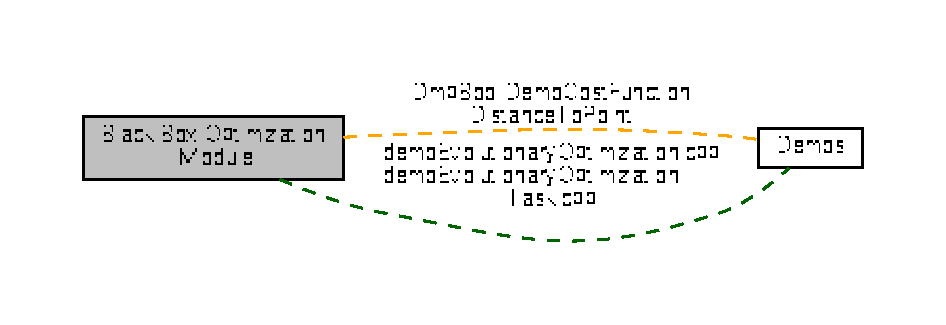
\includegraphics[width=350pt]{group__BBO}
\end{center}
\end{figure}
\subsubsection*{Files}
\begin{DoxyCompactItemize}
\item 
file \hyperlink{demoEvolutionaryOptimization_8cpp}{demo\+Evolutionary\+Optimization.\+cpp}
\begin{DoxyCompactList}\small\item\em Demonstrates how to run an evolution strategy to optimize a distance function, implemented as a Cost\+Function. \end{DoxyCompactList}\item 
file \hyperlink{demoEvolutionaryOptimizationTask_8cpp}{demo\+Evolutionary\+Optimization\+Task.\+cpp}
\begin{DoxyCompactList}\small\item\em Demonstrates how to run an evolution strategy to optimize the parameters of a quadratic function, implemented as a Task and Task\+Solver. \end{DoxyCompactList}\end{DoxyCompactItemize}
\subsubsection*{Classes}
\begin{DoxyCompactItemize}
\item 
class \hyperlink{classDmpBbo_1_1DemoCostFunctionDistanceToPoint}{Demo\+Cost\+Function\+Distance\+To\+Point}
\begin{DoxyCompactList}\small\item\em \hyperlink{classDmpBbo_1_1CostFunction}{Cost\+Function} in which the distance to a pre-\/defined point must be minimized. \end{DoxyCompactList}\end{DoxyCompactItemize}


\subsubsection{Detailed Description}

\hypertarget{group__Dmps}{\subsection{Dynamic Movement Primitives}
\label{group__Dmps}\index{Dynamic Movement Primitives@{Dynamic Movement Primitives}}
}
Collaboration diagram for Dynamic Movement Primitives\+:
\nopagebreak
\begin{figure}[H]
\begin{center}
\leavevmode
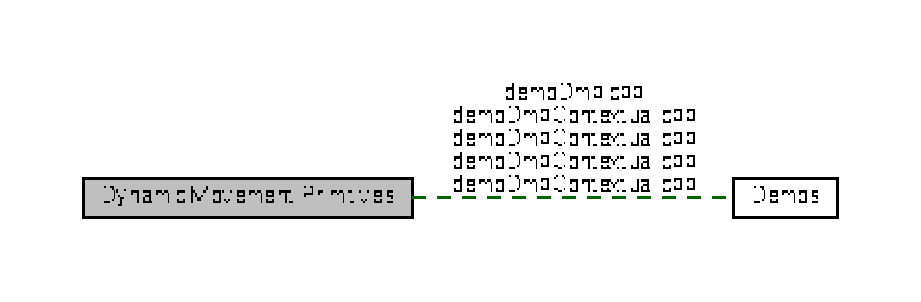
\includegraphics[width=350pt]{group__Dmps}
\end{center}
\end{figure}
\subsubsection*{Files}
\begin{DoxyCompactItemize}
\item 
file \hyperlink{demoDmp_8cpp}{demo\+Dmp.\+cpp}
\begin{DoxyCompactList}\small\item\em Demonstrates how to initialize, train and integrate a Dmp. \end{DoxyCompactList}\item 
file \hyperlink{demoDmpContextual_8cpp}{demo\+Dmp\+Contextual.\+cpp}
\begin{DoxyCompactList}\small\item\em Demonstrates how to initialize, train and integrate a Contextual Dmp. \end{DoxyCompactList}\item 
file \hyperlink{demoDmpContextual_8cpp}{demo\+Dmp\+Contextual.\+cpp}
\begin{DoxyCompactList}\small\item\em Demonstrates how to initialize, train and integrate a Contextual Dmp. \end{DoxyCompactList}\end{DoxyCompactItemize}
\subsubsection*{Classes}
\begin{DoxyCompactItemize}
\item 
class \hyperlink{classDmpBbo_1_1Dmp}{Dmp}
\begin{DoxyCompactList}\small\item\em Implementation of Dynamical Movement Primitives. \end{DoxyCompactList}\item 
class \hyperlink{classDmpBbo_1_1DmpContextual}{Dmp\+Contextual}
\begin{DoxyCompactList}\small\item\em Implementation of Contextual Dynamical Movement Primitives. \end{DoxyCompactList}\item 
class \hyperlink{classDmpBbo_1_1DmpContextualOneStep}{Dmp\+Contextual\+One\+Step}
\begin{DoxyCompactList}\small\item\em Implementation of Contextual Dynamical Movement Primitives. \end{DoxyCompactList}\item 
class \hyperlink{classDmpBbo_1_1DmpContextualTwoStep}{Dmp\+Contextual\+Two\+Step}
\begin{DoxyCompactList}\small\item\em Implementation of Contextual Dynamical Movement Primitives. \end{DoxyCompactList}\end{DoxyCompactItemize}
\subsubsection*{Enumerations}
\begin{DoxyCompactItemize}
\item 
enum \hyperlink{group__Dmps_gaccba8d09ec99ae66e469b3511bb232a4}{Dmp\+Type} \{ {\bfseries I\+J\+S\+P\+E\+E\+R\+T\+\_\+2002\+\_\+\+M\+O\+V\+E\+M\+E\+N\+T}, 
{\bfseries K\+U\+L\+V\+I\+C\+I\+U\+S\+\_\+2012\+\_\+\+J\+O\+I\+N\+I\+N\+G}, 
{\bfseries C\+O\+U\+N\+T\+D\+O\+W\+N\+\_\+2013}
 \}
\begin{DoxyCompactList}\small\item\em Different types of D\+M\+Ps that can be initialized. \end{DoxyCompactList}\end{DoxyCompactItemize}


\subsubsection{Detailed Description}


\subsubsection{Enumeration Type Documentation}
\hypertarget{group__Dmps_gaccba8d09ec99ae66e469b3511bb232a4}{\index{Dynamic Movement Primitives@{Dynamic Movement Primitives}!Dmp\+Type@{Dmp\+Type}}
\index{Dmp\+Type@{Dmp\+Type}!Dynamic Movement Primitives@{Dynamic Movement Primitives}}
\paragraph[{Dmp\+Type}]{\setlength{\rightskip}{0pt plus 5cm}enum Dmp\+Type}}\label{group__Dmps_gaccba8d09ec99ae66e469b3511bb232a4}


Different types of D\+M\+Ps that can be initialized. 



Definition at line 58 of file Dmp.\+hpp.


\begin{DoxyCode}
58 \{ IJSPEERT\_2002\_MOVEMENT, KULVICIUS\_2012\_JOINING, COUNTDOWN\_2013  \};
\end{DoxyCode}

\hypertarget{group__DMP__BBO}{\subsection{Black Box Optimization of Dynamical Movement Primitives Module}
\label{group__DMP__BBO}\index{Black Box Optimization of Dynamical Movement Primitives Module@{Black Box Optimization of Dynamical Movement Primitives Module}}
}

\hypertarget{group__DynamicalSystems}{\subsection{Dynamical Systems}
\label{group__DynamicalSystems}\index{Dynamical Systems@{Dynamical Systems}}
}
Collaboration diagram for Dynamical Systems\+:
\nopagebreak
\begin{figure}[H]
\begin{center}
\leavevmode
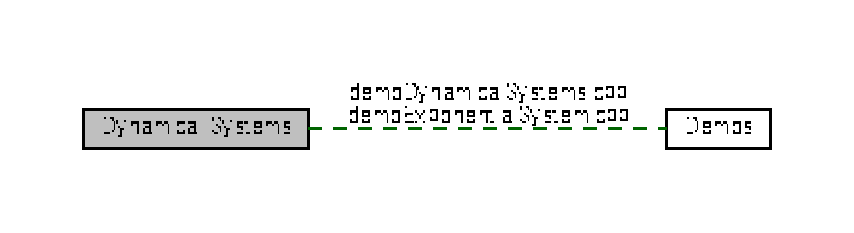
\includegraphics[width=350pt]{group__DynamicalSystems}
\end{center}
\end{figure}
\subsubsection*{Files}
\begin{DoxyCompactItemize}
\item 
file \hyperlink{demoDynamicalSystems_8cpp}{demo\+Dynamical\+Systems.\+cpp}
\begin{DoxyCompactList}\small\item\em Demonstrates how to initialize, integrate, perturb all implemented exponential systems. \end{DoxyCompactList}\item 
file \hyperlink{demoExponentialSystem_8cpp}{demo\+Exponential\+System.\+cpp}
\begin{DoxyCompactList}\small\item\em Demonstrates how to initialize and integrate an exponential dynamical system. \end{DoxyCompactList}\end{DoxyCompactItemize}
\subsubsection*{Classes}
\begin{DoxyCompactItemize}
\item 
class \hyperlink{classDmpBbo_1_1DynamicalSystem}{Dynamical\+System}
\begin{DoxyCompactList}\small\item\em Interface for implementing dynamical systems. \end{DoxyCompactList}\item 
class \hyperlink{classDmpBbo_1_1ExponentialSystem}{Exponential\+System}
\begin{DoxyCompactList}\small\item\em Dynamical System modelling the evolution of an exponential system\+: $\dot{x} = -\alpha (x-x^g)$. \end{DoxyCompactList}\item 
class \hyperlink{classDmpBbo_1_1SigmoidSystem}{Sigmoid\+System}
\begin{DoxyCompactList}\small\item\em Dynamical System modelling the evolution of a sigmoidal system $\dot{x} = -\alpha x(1-x/K)$. \end{DoxyCompactList}\item 
class \hyperlink{classDmpBbo_1_1SpringDamperSystem}{Spring\+Damper\+System}
\begin{DoxyCompactList}\small\item\em Dynamical System modelling the evolution of a spring-\/damper system\+: $ m\ddot{x} = -k(x-x^g) -c\dot{x}$. \end{DoxyCompactList}\item 
class \hyperlink{classDmpBbo_1_1TimeSystem}{Time\+System}
\begin{DoxyCompactList}\small\item\em Dynamical System modelling the evolution of a time\+: $\dot{x} = 1/\tau$. \end{DoxyCompactList}\end{DoxyCompactItemize}
\subsubsection*{Accessor functions}
\begin{DoxyCompactItemize}
\item 
enum \hyperlink{group__DynamicalSystems_ga9eca50997f7f604b063d2cb1874f5fef}{Integration\+Method} \{ {\bfseries E\+U\+L\+E\+R}, 
{\bfseries R\+U\+N\+G\+E\+\_\+\+K\+U\+T\+T\+A}
 \}
\begin{DoxyCompactList}\small\item\em The possible integration methods that can be used. \end{DoxyCompactList}\item 
void \hyperlink{group__DynamicalSystems_ga07a2df4cc46a521ab81c614d79b33669}{set\+\_\+integration\+\_\+method} (Integration\+Method integration\+\_\+method)
\begin{DoxyCompactList}\small\item\em Choose the integration method. \end{DoxyCompactList}\item 
int \hyperlink{group__DynamicalSystems_ga6f628f7f4ed9d77bf69f5b8560b98f18}{dim} (void) const 
\begin{DoxyCompactList}\small\item\em Get the dimensionality of the dynamical system, i.\+e. \end{DoxyCompactList}\item 
int \hyperlink{group__DynamicalSystems_ga93d7cbbf2e471b00f124e41706405a05}{dim\+\_\+orig} (void) const 
\begin{DoxyCompactList}\small\item\em Get the dimensionality of the dynamical system, i.\+e. \end{DoxyCompactList}\item 
double \hyperlink{group__DynamicalSystems_ga50eec7ad4c9664b5809ace45b22200d5}{tau} (void) const 
\begin{DoxyCompactList}\small\item\em Accessor function for the time constant. \end{DoxyCompactList}\item 
virtual void \hyperlink{group__DynamicalSystems_ga91155da280310b176cbd5fc1627820c7}{set\+\_\+tau} (double tau)
\begin{DoxyCompactList}\small\item\em Mutator function for the time constant. \end{DoxyCompactList}\item 
Eigen\+::\+Vector\+Xd \hyperlink{group__DynamicalSystems_ga4c7f24e7deec1629548a075015bdc693}{initial\+\_\+state} (void) const 
\begin{DoxyCompactList}\small\item\em Accessor function for the initial state of the dynamical system. \end{DoxyCompactList}\item 
virtual void \hyperlink{group__DynamicalSystems_ga23f05bcccb6a5deda6d2a5364d8ebb16}{set\+\_\+initial\+\_\+state} (const Eigen\+::\+Vector\+Xd \&initial\+\_\+state)
\begin{DoxyCompactList}\small\item\em Mutator function for the initial state of the dynamical system. \end{DoxyCompactList}\item 
Eigen\+::\+Vector\+Xd \hyperlink{group__DynamicalSystems_gaebe3c462bc4a725cb17bcc3d13285f13}{attractor\+\_\+state} (void) const 
\begin{DoxyCompactList}\small\item\em Accessor function for the attractor state of the dynamical system. \end{DoxyCompactList}\item 
virtual void \hyperlink{group__DynamicalSystems_ga32a975e60b5f001308368c7f06b90e18}{set\+\_\+attractor\+\_\+state} (const Eigen\+::\+Vector\+Xd \&attractor\+\_\+state)
\begin{DoxyCompactList}\small\item\em Mutator function for the attractor state of the dynamical system. \end{DoxyCompactList}\item 
std\+::string \hyperlink{group__DynamicalSystems_gacd23346c798f78014a4f82c853e83c88}{name} (void) const 
\begin{DoxyCompactList}\small\item\em Accessor function for the name of the dynamical system. \end{DoxyCompactList}\item 
virtual void \hyperlink{group__DynamicalSystems_ga5175bca5f98f36690a79e323119a1529}{set\+\_\+name} (std\+::string name)
\begin{DoxyCompactList}\small\item\em Mutator function for the name of the dynamical system. \end{DoxyCompactList}\item 
void \hyperlink{group__DynamicalSystems_ga9000562e645149d75717458a97db6ff5}{set\+\_\+dim} (int dim)
\begin{DoxyCompactList}\small\item\em Set the dimensionality of the dynamical system, i.\+e. \end{DoxyCompactList}\end{DoxyCompactItemize}


\subsubsection{Detailed Description}


\subsubsection{Enumeration Type Documentation}
\hypertarget{group__DynamicalSystems_ga9eca50997f7f604b063d2cb1874f5fef}{\index{Dynamical Systems@{Dynamical Systems}!Integration\+Method@{Integration\+Method}}
\index{Integration\+Method@{Integration\+Method}!Dynamical Systems@{Dynamical Systems}}
\paragraph[{Integration\+Method}]{\setlength{\rightskip}{0pt plus 5cm}enum Integration\+Method}}\label{group__DynamicalSystems_ga9eca50997f7f604b063d2cb1874f5fef}


The possible integration methods that can be used. 

\begin{DoxyItemize}
\item E\+U\+L\+E\+R\+: simple Euler method (\href{http://en.wikipedia.org/wiki/Euler_integration}{\tt http\+://en.\+wikipedia.\+org/wiki/\+Euler\+\_\+integration}) \item R\+U\+N\+G\+E\+\_\+\+K\+U\+T\+T\+A\+: 4th-\/order Runge-\/\+Kutta (\href{http://en.wikipedia.org/wiki/List_of_Runge%E2%80%93Kutta_methods#Classic_fourth-order_method}{\tt http\+://en.\+wikipedia.\+org/wiki/\+List\+\_\+of\+\_\+\+Runge\%\+E2\%80\%93\+Kutta\+\_\+methods\#\+Classic\+\_\+fourth-\/order\+\_\+method}) \end{DoxyItemize}


Definition at line 185 of file Dynamical\+System.\+hpp.


\begin{DoxyCode}
185 \{ EULER, RUNGE\_KUTTA \};
\end{DoxyCode}


\subsubsection{Function Documentation}
\hypertarget{group__DynamicalSystems_ga07a2df4cc46a521ab81c614d79b33669}{\index{Dynamical Systems@{Dynamical Systems}!set\+\_\+integration\+\_\+method@{set\+\_\+integration\+\_\+method}}
\index{set\+\_\+integration\+\_\+method@{set\+\_\+integration\+\_\+method}!Dynamical Systems@{Dynamical Systems}}
\paragraph[{set\+\_\+integration\+\_\+method}]{\setlength{\rightskip}{0pt plus 5cm}void set\+\_\+integration\+\_\+method (
\begin{DoxyParamCaption}
\item[{{\bf Integration\+Method}}]{integration\+\_\+method}
\end{DoxyParamCaption}
)\hspace{0.3cm}{\ttfamily [inline]}}}\label{group__DynamicalSystems_ga07a2df4cc46a521ab81c614d79b33669}


Choose the integration method. 


\begin{DoxyParams}[1]{Parameters}
\mbox{\tt in}  & {\em integration\+\_\+method} & The integration method, see \hyperlink{group__DynamicalSystems_ga9eca50997f7f604b063d2cb1874f5fef}{Dynamical\+System\+::\+Integration\+Method}. \\
\hline
\end{DoxyParams}


Definition at line 190 of file Dynamical\+System.\+hpp.


\begin{DoxyCode}
190                                                                            \{
191     integration\_method\_ = integration\_method;
192   \}
\end{DoxyCode}
\hypertarget{group__DynamicalSystems_ga6f628f7f4ed9d77bf69f5b8560b98f18}{\index{Dynamical Systems@{Dynamical Systems}!dim@{dim}}
\index{dim@{dim}!Dynamical Systems@{Dynamical Systems}}
\paragraph[{dim}]{\setlength{\rightskip}{0pt plus 5cm}int dim (
\begin{DoxyParamCaption}
\item[{void}]{}
\end{DoxyParamCaption}
) const\hspace{0.3cm}{\ttfamily [inline]}}}\label{group__DynamicalSystems_ga6f628f7f4ed9d77bf69f5b8560b98f18}


Get the dimensionality of the dynamical system, i.\+e. 

the length of its state vector. \begin{DoxyReturn}{Returns}
Dimensionality of the dynamical system 
\end{DoxyReturn}


Definition at line 198 of file Dynamical\+System.\+hpp.


\begin{DoxyCode}
198                              \{
199     \textcolor{keywordflow}{return} dim\_;
200   \}
\end{DoxyCode}
\hypertarget{group__DynamicalSystems_ga93d7cbbf2e471b00f124e41706405a05}{\index{Dynamical Systems@{Dynamical Systems}!dim\+\_\+orig@{dim\+\_\+orig}}
\index{dim\+\_\+orig@{dim\+\_\+orig}!Dynamical Systems@{Dynamical Systems}}
\paragraph[{dim\+\_\+orig}]{\setlength{\rightskip}{0pt plus 5cm}int dim\+\_\+orig (
\begin{DoxyParamCaption}
\item[{void}]{}
\end{DoxyParamCaption}
) const\hspace{0.3cm}{\ttfamily [inline]}}}\label{group__DynamicalSystems_ga93d7cbbf2e471b00f124e41706405a05}


Get the dimensionality of the dynamical system, i.\+e. 

the length of its output.

2nd order systems are represented as 1st order systems with an expanded state. The \hyperlink{classDmpBbo_1_1SpringDamperSystem}{Spring\+Damper\+System} for instance is represented as x = \mbox{[}y z\mbox{]}, xd = \mbox{[}yd zd\mbox{]}. Dynamical\+System\+::get\+Dim returns dim(x) = dim(\mbox{[}y z\mbox{]}) = 2$\ast$dim(y) \hyperlink{group__DynamicalSystems_ga93d7cbbf2e471b00f124e41706405a05}{Dynamical\+System\+::dim\+\_\+orig} returns dim(y) = \hyperlink{group__DynamicalSystems_ga6f628f7f4ed9d77bf69f5b8560b98f18}{dim()}/2

For Dynamical Movement Primitives, \hyperlink{group__DynamicalSystems_ga93d7cbbf2e471b00f124e41706405a05}{dim\+\_\+orig()} may be for instance 3, if the output of the D\+M\+P represents x,y,z coordinates. However, \hyperlink{group__DynamicalSystems_ga6f628f7f4ed9d77bf69f5b8560b98f18}{dim()} will have a much larger dimensionality, because it also contains the variables of all the subsystems (phase system, gating system, etc.)

\begin{DoxyReturn}{Returns}
Original dimensionality of the dynamical system 
\end{DoxyReturn}


Definition at line 216 of file Dynamical\+System.\+hpp.


\begin{DoxyCode}
216                                    \{
217     \textcolor{keywordflow}{return} dim\_orig\_;
218    \}
\end{DoxyCode}
\hypertarget{group__DynamicalSystems_ga50eec7ad4c9664b5809ace45b22200d5}{\index{Dynamical Systems@{Dynamical Systems}!tau@{tau}}
\index{tau@{tau}!Dynamical Systems@{Dynamical Systems}}
\paragraph[{tau}]{\setlength{\rightskip}{0pt plus 5cm}double tau (
\begin{DoxyParamCaption}
\item[{void}]{}
\end{DoxyParamCaption}
) const\hspace{0.3cm}{\ttfamily [inline]}}}\label{group__DynamicalSystems_ga50eec7ad4c9664b5809ace45b22200d5}


Accessor function for the time constant. 

\begin{DoxyReturn}{Returns}
Time constant 
\end{DoxyReturn}


Definition at line 224 of file Dynamical\+System.\+hpp.


\begin{DoxyCode}
224 \{ \textcolor{keywordflow}{return} tau\_; \}
\end{DoxyCode}
\hypertarget{group__DynamicalSystems_ga91155da280310b176cbd5fc1627820c7}{\index{Dynamical Systems@{Dynamical Systems}!set\+\_\+tau@{set\+\_\+tau}}
\index{set\+\_\+tau@{set\+\_\+tau}!Dynamical Systems@{Dynamical Systems}}
\paragraph[{set\+\_\+tau}]{\setlength{\rightskip}{0pt plus 5cm}virtual void set\+\_\+tau (
\begin{DoxyParamCaption}
\item[{double}]{tau}
\end{DoxyParamCaption}
)\hspace{0.3cm}{\ttfamily [inline]}, {\ttfamily [virtual]}}}\label{group__DynamicalSystems_ga91155da280310b176cbd5fc1627820c7}


Mutator function for the time constant. 


\begin{DoxyParams}[1]{Parameters}
\mbox{\tt in}  & {\em tau} & Time constant \\
\hline
\end{DoxyParams}


Reimplemented in \hyperlink{classDmpBbo_1_1Dmp_a17edb45ef62a4ef7f8c78e4f8f68b249}{Dmp}, and \hyperlink{classDmpBbo_1_1SigmoidSystem_a17edb45ef62a4ef7f8c78e4f8f68b249}{Sigmoid\+System}.



Definition at line 230 of file Dynamical\+System.\+hpp.


\begin{DoxyCode}
230                                           \{
231     assert(\hyperlink{group__DynamicalSystems_ga50eec7ad4c9664b5809ace45b22200d5}{tau}>0.0);
232     tau\_ = \hyperlink{group__DynamicalSystems_ga50eec7ad4c9664b5809ace45b22200d5}{tau};
233   \}
\end{DoxyCode}


Here is the call graph for this function\+:
\nopagebreak
\begin{figure}[H]
\begin{center}
\leavevmode
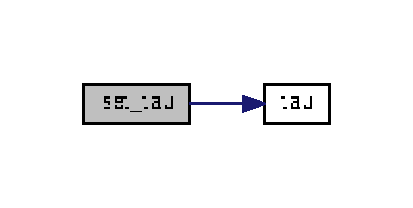
\includegraphics[width=198pt]{group__DynamicalSystems_ga91155da280310b176cbd5fc1627820c7_cgraph}
\end{center}
\end{figure}


\hypertarget{group__DynamicalSystems_ga4c7f24e7deec1629548a075015bdc693}{\index{Dynamical Systems@{Dynamical Systems}!initial\+\_\+state@{initial\+\_\+state}}
\index{initial\+\_\+state@{initial\+\_\+state}!Dynamical Systems@{Dynamical Systems}}
\paragraph[{initial\+\_\+state}]{\setlength{\rightskip}{0pt plus 5cm}Eigen\+::\+Vector\+Xd initial\+\_\+state (
\begin{DoxyParamCaption}
\item[{void}]{}
\end{DoxyParamCaption}
) const\hspace{0.3cm}{\ttfamily [inline]}}}\label{group__DynamicalSystems_ga4c7f24e7deec1629548a075015bdc693}


Accessor function for the initial state of the dynamical system. 

\begin{DoxyReturn}{Returns}
Initial state of the dynamical system. 
\end{DoxyReturn}


Definition at line 239 of file Dynamical\+System.\+hpp.


\begin{DoxyCode}
239 \{ \textcolor{keywordflow}{return} initial\_state\_; \}
\end{DoxyCode}
\hypertarget{group__DynamicalSystems_ga23f05bcccb6a5deda6d2a5364d8ebb16}{\index{Dynamical Systems@{Dynamical Systems}!set\+\_\+initial\+\_\+state@{set\+\_\+initial\+\_\+state}}
\index{set\+\_\+initial\+\_\+state@{set\+\_\+initial\+\_\+state}!Dynamical Systems@{Dynamical Systems}}
\paragraph[{set\+\_\+initial\+\_\+state}]{\setlength{\rightskip}{0pt plus 5cm}virtual void set\+\_\+initial\+\_\+state (
\begin{DoxyParamCaption}
\item[{const Eigen\+::\+Vector\+Xd \&}]{initial\+\_\+state}
\end{DoxyParamCaption}
)\hspace{0.3cm}{\ttfamily [inline]}, {\ttfamily [virtual]}}}\label{group__DynamicalSystems_ga23f05bcccb6a5deda6d2a5364d8ebb16}


Mutator function for the initial state of the dynamical system. 


\begin{DoxyParams}[1]{Parameters}
\mbox{\tt in}  & {\em initial\+\_\+state} & Initial state of the dynamical system. \\
\hline
\end{DoxyParams}


Reimplemented in \hyperlink{classDmpBbo_1_1Dmp_ad4e11c676c2add8a992db1caf542f0a0}{Dmp}, and \hyperlink{classDmpBbo_1_1SigmoidSystem_ad4e11c676c2add8a992db1caf542f0a0}{Sigmoid\+System}.



Definition at line 244 of file Dynamical\+System.\+hpp.


\begin{DoxyCode}
244                                                                             \{
245     assert(\hyperlink{group__DynamicalSystems_ga4c7f24e7deec1629548a075015bdc693}{initial\_state}.size()==dim\_orig\_);
246     initial\_state\_ = \hyperlink{group__DynamicalSystems_ga4c7f24e7deec1629548a075015bdc693}{initial\_state};
247   \}
\end{DoxyCode}


Here is the call graph for this function\+:
\nopagebreak
\begin{figure}[H]
\begin{center}
\leavevmode
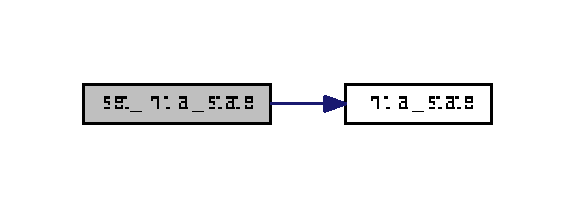
\includegraphics[width=276pt]{group__DynamicalSystems_ga23f05bcccb6a5deda6d2a5364d8ebb16_cgraph}
\end{center}
\end{figure}


\hypertarget{group__DynamicalSystems_gaebe3c462bc4a725cb17bcc3d13285f13}{\index{Dynamical Systems@{Dynamical Systems}!attractor\+\_\+state@{attractor\+\_\+state}}
\index{attractor\+\_\+state@{attractor\+\_\+state}!Dynamical Systems@{Dynamical Systems}}
\paragraph[{attractor\+\_\+state}]{\setlength{\rightskip}{0pt plus 5cm}Eigen\+::\+Vector\+Xd attractor\+\_\+state (
\begin{DoxyParamCaption}
\item[{void}]{}
\end{DoxyParamCaption}
) const\hspace{0.3cm}{\ttfamily [inline]}}}\label{group__DynamicalSystems_gaebe3c462bc4a725cb17bcc3d13285f13}


Accessor function for the attractor state of the dynamical system. 

\begin{DoxyReturn}{Returns}
Attractor state of the dynamical system. 
\end{DoxyReturn}


Definition at line 253 of file Dynamical\+System.\+hpp.


\begin{DoxyCode}
253 \{ \textcolor{keywordflow}{return} attractor\_state\_; \}
\end{DoxyCode}
\hypertarget{group__DynamicalSystems_ga32a975e60b5f001308368c7f06b90e18}{\index{Dynamical Systems@{Dynamical Systems}!set\+\_\+attractor\+\_\+state@{set\+\_\+attractor\+\_\+state}}
\index{set\+\_\+attractor\+\_\+state@{set\+\_\+attractor\+\_\+state}!Dynamical Systems@{Dynamical Systems}}
\paragraph[{set\+\_\+attractor\+\_\+state}]{\setlength{\rightskip}{0pt plus 5cm}virtual void set\+\_\+attractor\+\_\+state (
\begin{DoxyParamCaption}
\item[{const Eigen\+::\+Vector\+Xd \&}]{attractor\+\_\+state}
\end{DoxyParamCaption}
)\hspace{0.3cm}{\ttfamily [inline]}, {\ttfamily [virtual]}}}\label{group__DynamicalSystems_ga32a975e60b5f001308368c7f06b90e18}


Mutator function for the attractor state of the dynamical system. 


\begin{DoxyParams}[1]{Parameters}
\mbox{\tt in}  & {\em attractor\+\_\+state} & Attractor state of the dynamical system. \\
\hline
\end{DoxyParams}


Reimplemented in \hyperlink{classDmpBbo_1_1Dmp_a6dccbd077acfd148f528a48a72a4003f}{Dmp}.



Definition at line 258 of file Dynamical\+System.\+hpp.


\begin{DoxyCode}
258                                                                                 \{
259     assert(\hyperlink{group__DynamicalSystems_gaebe3c462bc4a725cb17bcc3d13285f13}{attractor\_state}.size()==dim\_orig\_);
260     attractor\_state\_ = \hyperlink{group__DynamicalSystems_gaebe3c462bc4a725cb17bcc3d13285f13}{attractor\_state};
261   \}
\end{DoxyCode}


Here is the call graph for this function\+:
\nopagebreak
\begin{figure}[H]
\begin{center}
\leavevmode
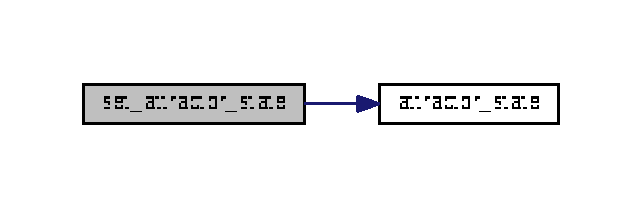
\includegraphics[width=308pt]{group__DynamicalSystems_ga32a975e60b5f001308368c7f06b90e18_cgraph}
\end{center}
\end{figure}


\hypertarget{group__DynamicalSystems_gacd23346c798f78014a4f82c853e83c88}{\index{Dynamical Systems@{Dynamical Systems}!name@{name}}
\index{name@{name}!Dynamical Systems@{Dynamical Systems}}
\paragraph[{name}]{\setlength{\rightskip}{0pt plus 5cm}std\+::string name (
\begin{DoxyParamCaption}
\item[{void}]{}
\end{DoxyParamCaption}
) const\hspace{0.3cm}{\ttfamily [inline]}}}\label{group__DynamicalSystems_gacd23346c798f78014a4f82c853e83c88}


Accessor function for the name of the dynamical system. 

\begin{DoxyReturn}{Returns}
Name of the dynamical system. 
\end{DoxyReturn}


Definition at line 267 of file Dynamical\+System.\+hpp.


\begin{DoxyCode}
267 \{ \textcolor{keywordflow}{return} name\_; \}
\end{DoxyCode}
\hypertarget{group__DynamicalSystems_ga5175bca5f98f36690a79e323119a1529}{\index{Dynamical Systems@{Dynamical Systems}!set\+\_\+name@{set\+\_\+name}}
\index{set\+\_\+name@{set\+\_\+name}!Dynamical Systems@{Dynamical Systems}}
\paragraph[{set\+\_\+name}]{\setlength{\rightskip}{0pt plus 5cm}virtual void set\+\_\+name (
\begin{DoxyParamCaption}
\item[{std\+::string}]{name}
\end{DoxyParamCaption}
)\hspace{0.3cm}{\ttfamily [inline]}, {\ttfamily [virtual]}}}\label{group__DynamicalSystems_ga5175bca5f98f36690a79e323119a1529}


Mutator function for the name of the dynamical system. 


\begin{DoxyParams}[1]{Parameters}
\mbox{\tt in}  & {\em name} & Name of the dynamical system. \\
\hline
\end{DoxyParams}


Definition at line 272 of file Dynamical\+System.\+hpp.


\begin{DoxyCode}
272                                                \{
273     name\_ = \hyperlink{group__DynamicalSystems_gacd23346c798f78014a4f82c853e83c88}{name};
274   \}
\end{DoxyCode}


Here is the call graph for this function\+:
\nopagebreak
\begin{figure}[H]
\begin{center}
\leavevmode
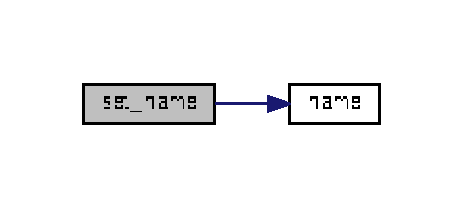
\includegraphics[width=222pt]{group__DynamicalSystems_ga5175bca5f98f36690a79e323119a1529_cgraph}
\end{center}
\end{figure}


\hypertarget{group__DynamicalSystems_ga9000562e645149d75717458a97db6ff5}{\index{Dynamical Systems@{Dynamical Systems}!set\+\_\+dim@{set\+\_\+dim}}
\index{set\+\_\+dim@{set\+\_\+dim}!Dynamical Systems@{Dynamical Systems}}
\paragraph[{set\+\_\+dim}]{\setlength{\rightskip}{0pt plus 5cm}void set\+\_\+dim (
\begin{DoxyParamCaption}
\item[{int}]{dim}
\end{DoxyParamCaption}
)\hspace{0.3cm}{\ttfamily [inline]}, {\ttfamily [protected]}}}\label{group__DynamicalSystems_ga9000562e645149d75717458a97db6ff5}


Set the dimensionality of the dynamical system, i.\+e. 

the length of its state vector. 
\begin{DoxyParams}[1]{Parameters}
\mbox{\tt in}  & {\em dim} & Dimensionality of the dynamical system \\
\hline
\end{DoxyParams}


Definition at line 281 of file Dynamical\+System.\+hpp.


\begin{DoxyCode}
281                                \{
282     dim\_ = \hyperlink{group__DynamicalSystems_ga6f628f7f4ed9d77bf69f5b8560b98f18}{dim};
283   \}
\end{DoxyCode}


Here is the call graph for this function\+:
\nopagebreak
\begin{figure}[H]
\begin{center}
\leavevmode
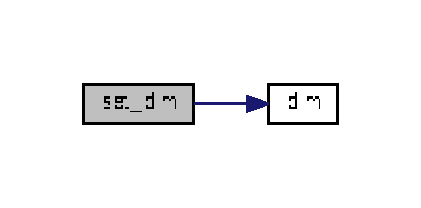
\includegraphics[width=202pt]{group__DynamicalSystems_ga9000562e645149d75717458a97db6ff5_cgraph}
\end{center}
\end{figure}



\hypertarget{group__FunctionApproximators}{\subsection{Function Approximators}
\label{group__FunctionApproximators}\index{Function Approximators@{Function Approximators}}
}
Collaboration diagram for Function Approximators\+:
\nopagebreak
\begin{figure}[H]
\begin{center}
\leavevmode
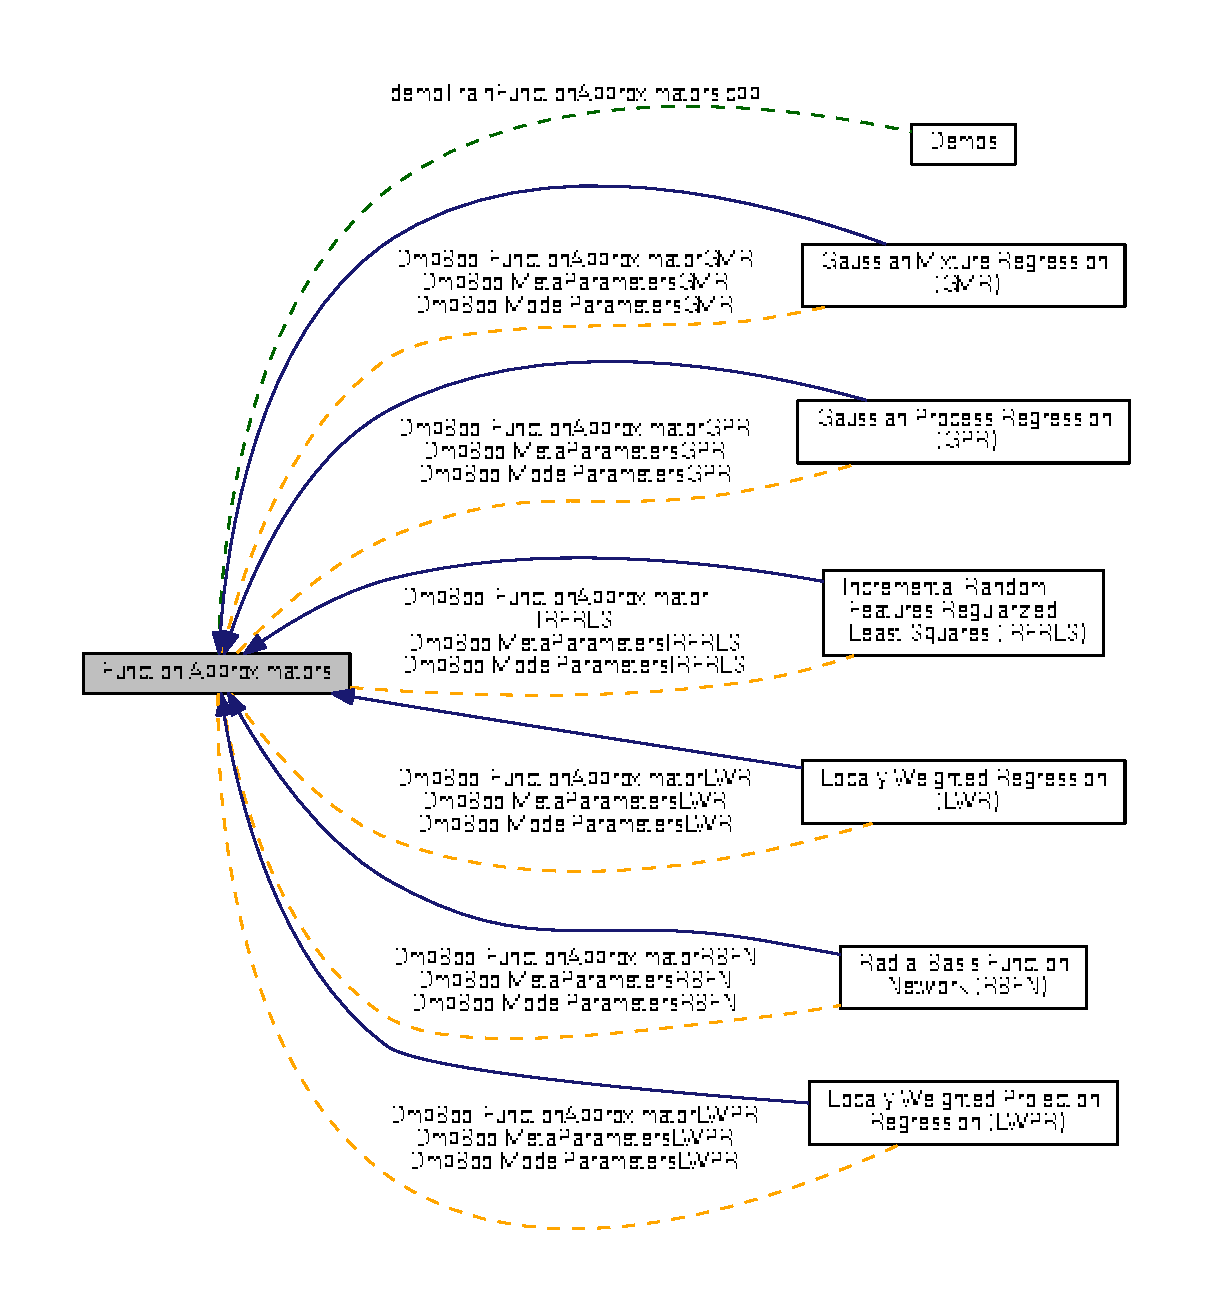
\includegraphics[width=350pt]{group__FunctionApproximators}
\end{center}
\end{figure}
\subsubsection*{Modules}
\begin{DoxyCompactItemize}
\item 
\hyperlink{group__GMR}{Gaussian Mixture Regression (\+G\+M\+R)}
\item 
\hyperlink{group__GPR}{Gaussian Process Regression (\+G\+P\+R)}
\item 
\hyperlink{group__IRFRLS}{Incremental Random Features Regularized Least Squares (i\+R\+F\+R\+L\+S)}
\item 
\hyperlink{group__LWPR}{Locally Weighted Projection Regression (\+L\+W\+P\+R)}
\item 
\hyperlink{group__LWR}{Locally Weighted Regression (\+L\+W\+R)}
\item 
\hyperlink{group__RBFN}{Radial Basis Function Network (\+R\+B\+F\+N)}
\end{DoxyCompactItemize}
\subsubsection*{Files}
\begin{DoxyCompactItemize}
\item 
file \hyperlink{demoTrainFunctionApproximators_8cpp}{demo\+Train\+Function\+Approximators.\+cpp}
\begin{DoxyCompactList}\small\item\em Demonstrates how to initialize and train a function approximator.. \end{DoxyCompactList}\end{DoxyCompactItemize}
\subsubsection*{Classes}
\begin{DoxyCompactItemize}
\item 
class \hyperlink{classDmpBbo_1_1FunctionApproximator}{Function\+Approximator}
\begin{DoxyCompactList}\small\item\em Base class for all function approximators. \end{DoxyCompactList}\item 
class \hyperlink{classDmpBbo_1_1FunctionApproximatorGMR}{Function\+Approximator\+G\+M\+R}
\begin{DoxyCompactList}\small\item\em G\+M\+R (Gaussian Mixture Regression) function approximator. \end{DoxyCompactList}\item 
class \hyperlink{classDmpBbo_1_1FunctionApproximatorGPR}{Function\+Approximator\+G\+P\+R}
\begin{DoxyCompactList}\small\item\em G\+P\+R (Gaussian Process Regression) function approximator. \end{DoxyCompactList}\item 
class \hyperlink{classDmpBbo_1_1FunctionApproximatorIRFRLS}{Function\+Approximator\+I\+R\+F\+R\+L\+S}
\begin{DoxyCompactList}\small\item\em i\+R\+F\+R\+L\+S (Incremental Random Features Regularized Least Squares) function approximator \end{DoxyCompactList}\item 
class \hyperlink{classDmpBbo_1_1FunctionApproximatorLWPR}{Function\+Approximator\+L\+W\+P\+R}
\begin{DoxyCompactList}\small\item\em L\+W\+P\+R (Locally Weighted Projection Regression) function approximator. \end{DoxyCompactList}\item 
class \hyperlink{classDmpBbo_1_1FunctionApproximatorLWR}{Function\+Approximator\+L\+W\+R}
\begin{DoxyCompactList}\small\item\em L\+W\+R (Locally Weighted Regression) function approximator. \end{DoxyCompactList}\item 
class \hyperlink{classDmpBbo_1_1FunctionApproximatorRBFN}{Function\+Approximator\+R\+B\+F\+N}
\begin{DoxyCompactList}\small\item\em R\+B\+F\+N (Radial Basis Function Network) function approximator. \end{DoxyCompactList}\item 
class \hyperlink{classDmpBbo_1_1MetaParameters}{Meta\+Parameters}
\begin{DoxyCompactList}\small\item\em Base class for all meta-\/parameters of function approximators. \end{DoxyCompactList}\item 
class \hyperlink{classDmpBbo_1_1MetaParametersGMR}{Meta\+Parameters\+G\+M\+R}
\begin{DoxyCompactList}\small\item\em Meta-\/parameters for the G\+M\+R function approximator. \end{DoxyCompactList}\item 
class \hyperlink{classDmpBbo_1_1MetaParametersGPR}{Meta\+Parameters\+G\+P\+R}
\begin{DoxyCompactList}\small\item\em Meta-\/parameters for the Gaussian Process Regression (G\+P\+R) function approximator. \end{DoxyCompactList}\item 
class \hyperlink{classDmpBbo_1_1MetaParametersIRFRLS}{Meta\+Parameters\+I\+R\+F\+R\+L\+S}
\begin{DoxyCompactList}\small\item\em Meta-\/parameters for the i\+R\+F\+R\+L\+S function approximator. \end{DoxyCompactList}\item 
class \hyperlink{classDmpBbo_1_1MetaParametersLWPR}{Meta\+Parameters\+L\+W\+P\+R}
\begin{DoxyCompactList}\small\item\em Meta-\/parameters for the Locally Weighted Projection Regression (L\+W\+P\+R) function approximator. \end{DoxyCompactList}\item 
class \hyperlink{classDmpBbo_1_1MetaParametersLWR}{Meta\+Parameters\+L\+W\+R}
\begin{DoxyCompactList}\small\item\em Meta-\/parameters for the Locally Weighted Regression (L\+W\+R) function approximator. \end{DoxyCompactList}\item 
class \hyperlink{classDmpBbo_1_1MetaParametersRBFN}{Meta\+Parameters\+R\+B\+F\+N}
\begin{DoxyCompactList}\small\item\em Meta-\/parameters for the Radial Basis Function Network (R\+B\+F\+N) function approximator. \end{DoxyCompactList}\item 
class \hyperlink{classDmpBbo_1_1ModelParameters}{Model\+Parameters}
\begin{DoxyCompactList}\small\item\em Base class for all model parameters of function approximators. \end{DoxyCompactList}\item 
class \hyperlink{classDmpBbo_1_1ModelParametersGMR}{Model\+Parameters\+G\+M\+R}
\begin{DoxyCompactList}\small\item\em Model parameters for the G\+M\+R function approximator. \end{DoxyCompactList}\item 
class \hyperlink{classDmpBbo_1_1ModelParametersGPR}{Model\+Parameters\+G\+P\+R}
\begin{DoxyCompactList}\small\item\em Model parameters for the Gaussian Process Regression (G\+P\+R) function approximator. \end{DoxyCompactList}\item 
class \hyperlink{classDmpBbo_1_1ModelParametersIRFRLS}{Model\+Parameters\+I\+R\+F\+R\+L\+S}
\begin{DoxyCompactList}\small\item\em Model parameters for the i\+R\+F\+R\+L\+S function approximator. \end{DoxyCompactList}\item 
class \hyperlink{classDmpBbo_1_1ModelParametersLWPR}{Model\+Parameters\+L\+W\+P\+R}
\begin{DoxyCompactList}\small\item\em Model parameters for the Locally Weighted Projection Regression (L\+W\+P\+R) function approximator. \end{DoxyCompactList}\item 
class \hyperlink{classDmpBbo_1_1ModelParametersLWR}{Model\+Parameters\+L\+W\+R}
\begin{DoxyCompactList}\small\item\em Model parameters for the Locally Weighted Regression (L\+W\+R) function approximator. \end{DoxyCompactList}\item 
class \hyperlink{classDmpBbo_1_1ModelParametersRBFN}{Model\+Parameters\+R\+B\+F\+N}
\begin{DoxyCompactList}\small\item\em Model parameters for the Radial Basis Function Network (R\+B\+F\+N) function approximator. \end{DoxyCompactList}\item 
class \hyperlink{classDmpBbo_1_1UnifiedModel}{Unified\+Model}
\begin{DoxyCompactList}\small\item\em The unified model, which can be used to represent the model of all other function approximators. \end{DoxyCompactList}\end{DoxyCompactItemize}


\subsubsection{Detailed Description}

\hypertarget{group__GMR}{\subsection{Gaussian Mixture Regression (G\+M\+R)}
\label{group__GMR}\index{Gaussian Mixture Regression (\+G\+M\+R)@{Gaussian Mixture Regression (\+G\+M\+R)}}
}
Collaboration diagram for Gaussian Mixture Regression (G\+M\+R)\+:
\nopagebreak
\begin{figure}[H]
\begin{center}
\leavevmode
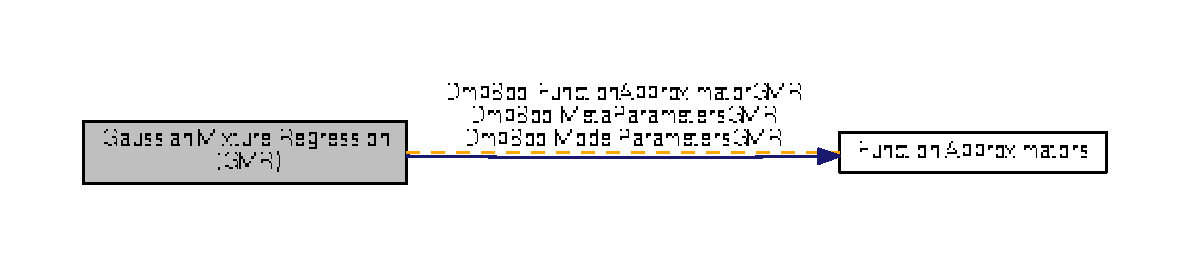
\includegraphics[width=350pt]{group__GMR}
\end{center}
\end{figure}
\subsubsection*{Classes}
\begin{DoxyCompactItemize}
\item 
class \hyperlink{classDmpBbo_1_1FunctionApproximatorGMR}{Function\+Approximator\+G\+M\+R}
\begin{DoxyCompactList}\small\item\em G\+M\+R (Gaussian Mixture Regression) function approximator. \end{DoxyCompactList}\item 
class \hyperlink{classDmpBbo_1_1MetaParametersGMR}{Meta\+Parameters\+G\+M\+R}
\begin{DoxyCompactList}\small\item\em Meta-\/parameters for the G\+M\+R function approximator. \end{DoxyCompactList}\item 
class \hyperlink{classDmpBbo_1_1ModelParametersGMR}{Model\+Parameters\+G\+M\+R}
\begin{DoxyCompactList}\small\item\em Model parameters for the G\+M\+R function approximator. \end{DoxyCompactList}\end{DoxyCompactItemize}


\subsubsection{Detailed Description}

\hypertarget{group__GPR}{\subsection{Gaussian Process Regression (G\+P\+R)}
\label{group__GPR}\index{Gaussian Process Regression (\+G\+P\+R)@{Gaussian Process Regression (\+G\+P\+R)}}
}
Collaboration diagram for Gaussian Process Regression (G\+P\+R)\+:
\nopagebreak
\begin{figure}[H]
\begin{center}
\leavevmode
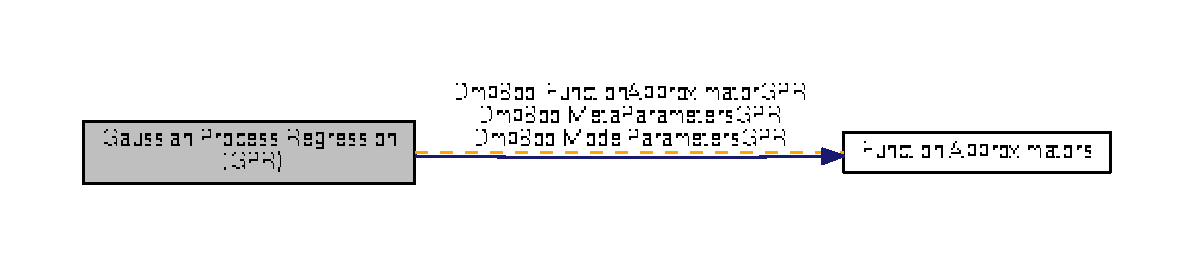
\includegraphics[width=350pt]{group__GPR}
\end{center}
\end{figure}
\subsubsection*{Classes}
\begin{DoxyCompactItemize}
\item 
class \hyperlink{classDmpBbo_1_1FunctionApproximatorGPR}{Function\+Approximator\+G\+P\+R}
\begin{DoxyCompactList}\small\item\em G\+P\+R (Gaussian Process Regression) function approximator. \end{DoxyCompactList}\item 
class \hyperlink{classDmpBbo_1_1MetaParametersGPR}{Meta\+Parameters\+G\+P\+R}
\begin{DoxyCompactList}\small\item\em Meta-\/parameters for the Gaussian Process Regression (G\+P\+R) function approximator. \end{DoxyCompactList}\item 
class \hyperlink{classDmpBbo_1_1ModelParametersGPR}{Model\+Parameters\+G\+P\+R}
\begin{DoxyCompactList}\small\item\em Model parameters for the Gaussian Process Regression (G\+P\+R) function approximator. \end{DoxyCompactList}\end{DoxyCompactItemize}


\subsubsection{Detailed Description}

\hypertarget{group__IRFRLS}{\subsection{Incremental Random Features Regularized Least Squares (i\+R\+F\+R\+L\+S)}
\label{group__IRFRLS}\index{Incremental Random Features Regularized Least Squares (i\+R\+F\+R\+L\+S)@{Incremental Random Features Regularized Least Squares (i\+R\+F\+R\+L\+S)}}
}
Collaboration diagram for Incremental Random Features Regularized Least Squares (i\+R\+F\+R\+L\+S)\+:
\nopagebreak
\begin{figure}[H]
\begin{center}
\leavevmode
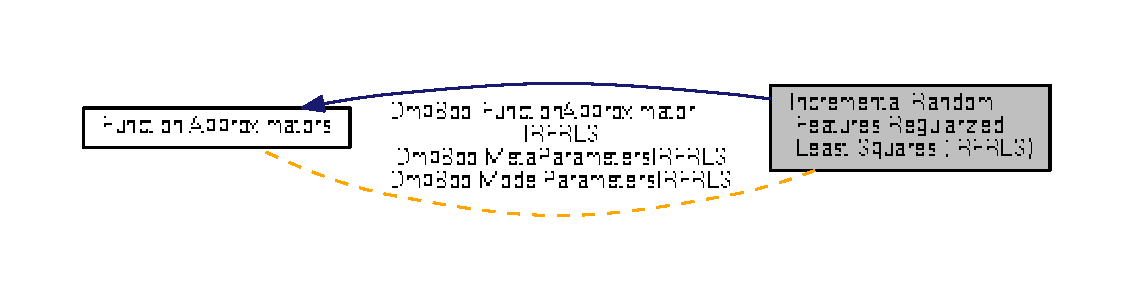
\includegraphics[width=350pt]{group__IRFRLS}
\end{center}
\end{figure}
\subsubsection*{Classes}
\begin{DoxyCompactItemize}
\item 
class \hyperlink{classDmpBbo_1_1FunctionApproximatorIRFRLS}{Function\+Approximator\+I\+R\+F\+R\+L\+S}
\begin{DoxyCompactList}\small\item\em i\+R\+F\+R\+L\+S (Incremental Random Features Regularized Least Squares) function approximator \end{DoxyCompactList}\item 
class \hyperlink{classDmpBbo_1_1MetaParametersIRFRLS}{Meta\+Parameters\+I\+R\+F\+R\+L\+S}
\begin{DoxyCompactList}\small\item\em Meta-\/parameters for the i\+R\+F\+R\+L\+S function approximator. \end{DoxyCompactList}\item 
class \hyperlink{classDmpBbo_1_1ModelParametersIRFRLS}{Model\+Parameters\+I\+R\+F\+R\+L\+S}
\begin{DoxyCompactList}\small\item\em Model parameters for the i\+R\+F\+R\+L\+S function approximator. \end{DoxyCompactList}\end{DoxyCompactItemize}


\subsubsection{Detailed Description}

\hypertarget{group__LWPR}{\subsection{Locally Weighted Projection Regression (L\+W\+P\+R)}
\label{group__LWPR}\index{Locally Weighted Projection Regression (\+L\+W\+P\+R)@{Locally Weighted Projection Regression (\+L\+W\+P\+R)}}
}
Collaboration diagram for Locally Weighted Projection Regression (L\+W\+P\+R)\+:
\nopagebreak
\begin{figure}[H]
\begin{center}
\leavevmode
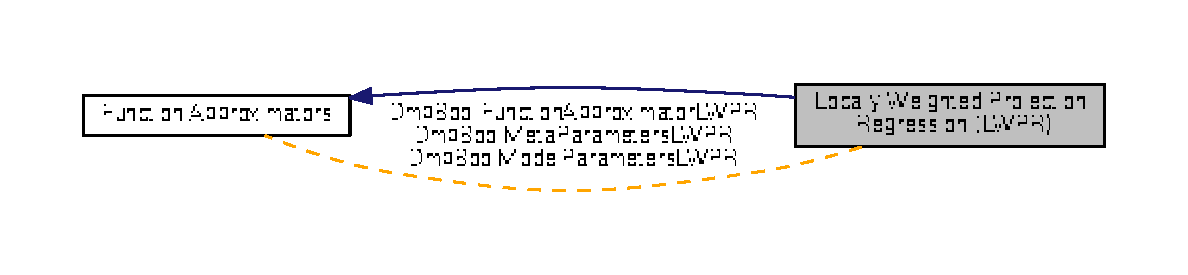
\includegraphics[width=350pt]{group__LWPR}
\end{center}
\end{figure}
\subsubsection*{Classes}
\begin{DoxyCompactItemize}
\item 
class \hyperlink{classDmpBbo_1_1FunctionApproximatorLWPR}{Function\+Approximator\+L\+W\+P\+R}
\begin{DoxyCompactList}\small\item\em L\+W\+P\+R (Locally Weighted Projection Regression) function approximator. \end{DoxyCompactList}\item 
class \hyperlink{classDmpBbo_1_1MetaParametersLWPR}{Meta\+Parameters\+L\+W\+P\+R}
\begin{DoxyCompactList}\small\item\em Meta-\/parameters for the Locally Weighted Projection Regression (L\+W\+P\+R) function approximator. \end{DoxyCompactList}\item 
class \hyperlink{classDmpBbo_1_1ModelParametersLWPR}{Model\+Parameters\+L\+W\+P\+R}
\begin{DoxyCompactList}\small\item\em Model parameters for the Locally Weighted Projection Regression (L\+W\+P\+R) function approximator. \end{DoxyCompactList}\end{DoxyCompactItemize}


\subsubsection{Detailed Description}

\hypertarget{group__LWR}{\subsection{Locally Weighted Regression (L\+W\+R)}
\label{group__LWR}\index{Locally Weighted Regression (\+L\+W\+R)@{Locally Weighted Regression (\+L\+W\+R)}}
}
Collaboration diagram for Locally Weighted Regression (L\+W\+R)\+:
\nopagebreak
\begin{figure}[H]
\begin{center}
\leavevmode
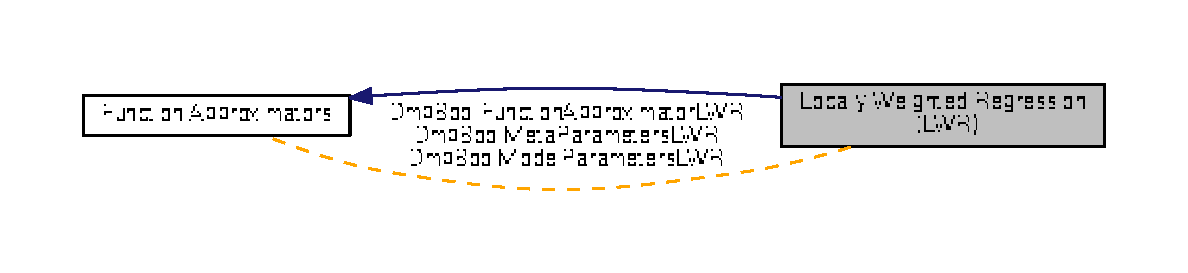
\includegraphics[width=350pt]{group__LWR}
\end{center}
\end{figure}
\subsubsection*{Classes}
\begin{DoxyCompactItemize}
\item 
class \hyperlink{classDmpBbo_1_1FunctionApproximatorLWR}{Function\+Approximator\+L\+W\+R}
\begin{DoxyCompactList}\small\item\em L\+W\+R (Locally Weighted Regression) function approximator. \end{DoxyCompactList}\item 
class \hyperlink{classDmpBbo_1_1MetaParametersLWR}{Meta\+Parameters\+L\+W\+R}
\begin{DoxyCompactList}\small\item\em Meta-\/parameters for the Locally Weighted Regression (L\+W\+R) function approximator. \end{DoxyCompactList}\item 
class \hyperlink{classDmpBbo_1_1ModelParametersLWR}{Model\+Parameters\+L\+W\+R}
\begin{DoxyCompactList}\small\item\em Model parameters for the Locally Weighted Regression (L\+W\+R) function approximator. \end{DoxyCompactList}\end{DoxyCompactItemize}


\subsubsection{Detailed Description}

\hypertarget{group__RBFN}{\subsection{Radial Basis Function Network (R\+B\+F\+N)}
\label{group__RBFN}\index{Radial Basis Function Network (\+R\+B\+F\+N)@{Radial Basis Function Network (\+R\+B\+F\+N)}}
}
Collaboration diagram for Radial Basis Function Network (R\+B\+F\+N)\+:
\nopagebreak
\begin{figure}[H]
\begin{center}
\leavevmode
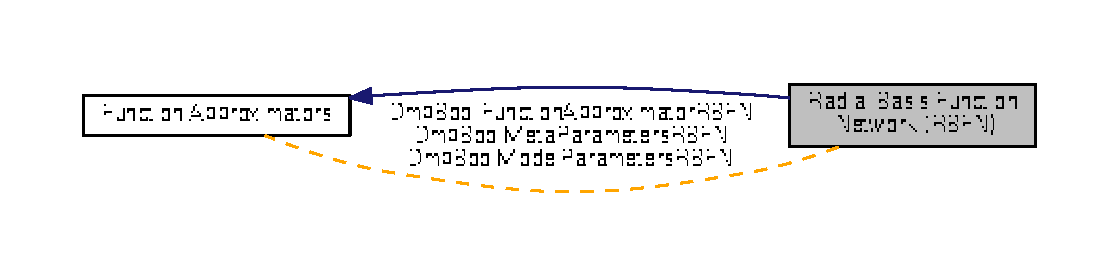
\includegraphics[width=350pt]{group__RBFN}
\end{center}
\end{figure}
\subsubsection*{Classes}
\begin{DoxyCompactItemize}
\item 
class \hyperlink{classDmpBbo_1_1FunctionApproximatorRBFN}{Function\+Approximator\+R\+B\+F\+N}
\begin{DoxyCompactList}\small\item\em R\+B\+F\+N (Radial Basis Function Network) function approximator. \end{DoxyCompactList}\item 
class \hyperlink{classDmpBbo_1_1MetaParametersRBFN}{Meta\+Parameters\+R\+B\+F\+N}
\begin{DoxyCompactList}\small\item\em Meta-\/parameters for the Radial Basis Function Network (R\+B\+F\+N) function approximator. \end{DoxyCompactList}\item 
class \hyperlink{classDmpBbo_1_1ModelParametersRBFN}{Model\+Parameters\+R\+B\+F\+N}
\begin{DoxyCompactList}\small\item\em Model parameters for the Radial Basis Function Network (R\+B\+F\+N) function approximator. \end{DoxyCompactList}\end{DoxyCompactItemize}


\subsubsection{Detailed Description}

\hypertarget{group__Demos}{\subsection{Demos}
\label{group__Demos}\index{Demos@{Demos}}
}
Collaboration diagram for Demos\+:
\nopagebreak
\begin{figure}[H]
\begin{center}
\leavevmode
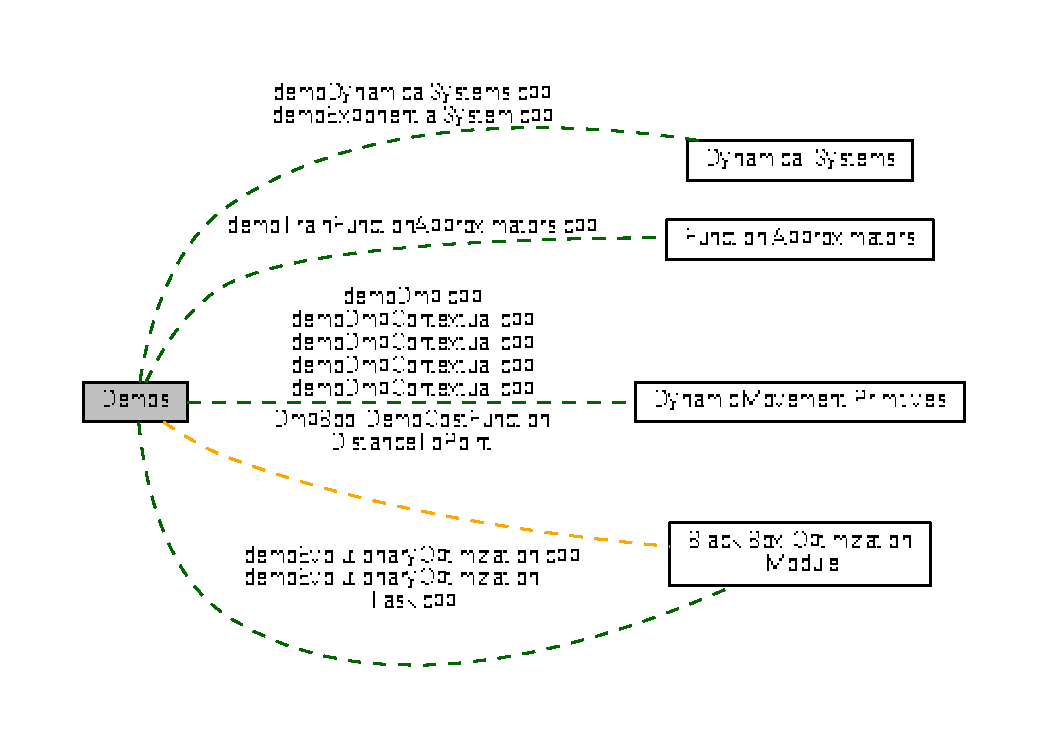
\includegraphics[width=350pt]{group__Demos}
\end{center}
\end{figure}
\subsubsection*{Files}
\begin{DoxyCompactItemize}
\item 
file \hyperlink{demoEvolutionaryOptimization_8cpp}{demo\+Evolutionary\+Optimization.\+cpp}
\begin{DoxyCompactList}\small\item\em Demonstrates how to run an evolution strategy to optimize a distance function, implemented as a Cost\+Function. \end{DoxyCompactList}\item 
file \hyperlink{demoEvolutionaryOptimizationTask_8cpp}{demo\+Evolutionary\+Optimization\+Task.\+cpp}
\begin{DoxyCompactList}\small\item\em Demonstrates how to run an evolution strategy to optimize the parameters of a quadratic function, implemented as a Task and Task\+Solver. \end{DoxyCompactList}\item 
file \hyperlink{demoDmp_8cpp}{demo\+Dmp.\+cpp}
\begin{DoxyCompactList}\small\item\em Demonstrates how to initialize, train and integrate a Dmp. \end{DoxyCompactList}\item 
file \hyperlink{demoDmpContextual_8cpp}{demo\+Dmp\+Contextual.\+cpp}
\begin{DoxyCompactList}\small\item\em Demonstrates how to initialize, train and integrate a Contextual Dmp. \end{DoxyCompactList}\item 
file \hyperlink{demoDmpContextual_8cpp}{demo\+Dmp\+Contextual.\+cpp}
\begin{DoxyCompactList}\small\item\em Demonstrates how to initialize, train and integrate a Contextual Dmp. \end{DoxyCompactList}\item 
file \hyperlink{demoDmpBbo_8cpp}{demo\+Dmp\+Bbo.\+cpp}
\begin{DoxyCompactList}\small\item\em Demonstrates how to run an evolution strategy to optimize a Dmp. \end{DoxyCompactList}\item 
file \hyperlink{demoDmpBboMultiDim_8cpp}{demo\+Dmp\+Bbo\+Multi\+Dim.\+cpp}
\begin{DoxyCompactList}\small\item\em Demonstrates how to run multiple evolution strategies in parallel to optimize a Dmp. \end{DoxyCompactList}\item 
file \hyperlink{demoImitationAndOptimization_8cpp}{demo\+Imitation\+And\+Optimization.\+cpp}
\begin{DoxyCompactList}\small\item\em Demonstrates how to initialize a D\+M\+P, and then optimize it with an evolution strategy. \end{DoxyCompactList}\item 
file \hyperlink{demoDynamicalSystems_8cpp}{demo\+Dynamical\+Systems.\+cpp}
\begin{DoxyCompactList}\small\item\em Demonstrates how to initialize, integrate, perturb all implemented exponential systems. \end{DoxyCompactList}\item 
file \hyperlink{demoExponentialSystem_8cpp}{demo\+Exponential\+System.\+cpp}
\begin{DoxyCompactList}\small\item\em Demonstrates how to initialize and integrate an exponential dynamical system. \end{DoxyCompactList}\item 
file \hyperlink{demoTrainFunctionApproximators_8cpp}{demo\+Train\+Function\+Approximators.\+cpp}
\begin{DoxyCompactList}\small\item\em Demonstrates how to initialize and train a function approximator.. \end{DoxyCompactList}\end{DoxyCompactItemize}
\subsubsection*{Classes}
\begin{DoxyCompactItemize}
\item 
class \hyperlink{classDmpBbo_1_1DemoCostFunctionDistanceToPoint}{Demo\+Cost\+Function\+Distance\+To\+Point}
\begin{DoxyCompactList}\small\item\em \hyperlink{classDmpBbo_1_1CostFunction}{Cost\+Function} in which the distance to a pre-\/defined point must be minimized. \end{DoxyCompactList}\end{DoxyCompactItemize}


\subsubsection{Detailed Description}

\section{Namespace Documentation}
\hypertarget{namespaceboost}{\subsection{boost Namespace Reference}
\label{namespaceboost}\index{boost@{boost}}
}


Serialization function for boost\+::serialization.  




\subsubsection{Detailed Description}
Serialization function for boost\+::serialization. 


\hypertarget{namespaceDmpBBO}{\subsection{Dmp\+B\+B\+O Namespace Reference}
\label{namespaceDmpBBO}\index{Dmp\+B\+B\+O@{Dmp\+B\+B\+O}}
}


Namespace used for all classes in the project.  




\subsubsection{Detailed Description}
Namespace used for all classes in the project. 
\section{Class Documentation}
\hypertarget{classDmpBbo_1_1CostFunction}{\subsection{Cost\+Function Class Reference}
\label{classDmpBbo_1_1CostFunction}\index{Cost\+Function@{Cost\+Function}}
}


Interface for cost functions, which define a cost\+\_\+function.  




{\ttfamily \#include $<$Cost\+Function.\+hpp$>$}



Inheritance diagram for Cost\+Function\+:
\nopagebreak
\begin{figure}[H]
\begin{center}
\leavevmode
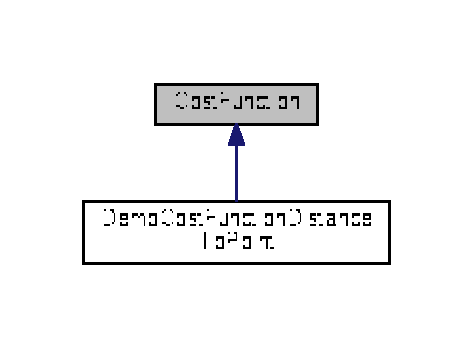
\includegraphics[width=227pt]{classDmpBbo_1_1CostFunction__inherit__graph}
\end{center}
\end{figure}
\subsubsection*{Public Member Functions}
\begin{DoxyCompactItemize}
\item 
virtual void \hyperlink{classDmpBbo_1_1CostFunction_a4468247a33250384422560fce57bf2ed}{evaluate} (const Eigen\+::\+Matrix\+Xd \&samples, Eigen\+::\+Vector\+Xd \&costs) const =0
\begin{DoxyCompactList}\small\item\em The cost function which defines the cost\+\_\+function. \end{DoxyCompactList}\item 
virtual std\+::string \hyperlink{classDmpBbo_1_1CostFunction_af084bff2ddd6233e9a898faa23f6195c}{to\+String} (void) const =0
\begin{DoxyCompactList}\small\item\em Returns a string representation of the object. \end{DoxyCompactList}\end{DoxyCompactItemize}
\subsubsection*{Friends}
\begin{DoxyCompactItemize}
\item 
std\+::ostream \& \hyperlink{classDmpBbo_1_1CostFunction_a664776318997dd7921e272845e0e1ecc}{operator$<$$<$} (std\+::ostream \&output, const \hyperlink{classDmpBbo_1_1CostFunction}{Cost\+Function} \&cost\+\_\+function)
\begin{DoxyCompactList}\small\item\em Write to output stream. \end{DoxyCompactList}\end{DoxyCompactItemize}


\subsubsection{Detailed Description}
Interface for cost functions, which define a cost\+\_\+function. 

For further information see the section on \hyperlink{page_bbo_sec_bbo_task_and_task_solver}{Cost\+Function vs Task/\+Task\+Solver} 

Definition at line 35 of file Cost\+Function.\+hpp.



\subsubsection{Member Function Documentation}
\hypertarget{classDmpBbo_1_1CostFunction_a4468247a33250384422560fce57bf2ed}{\index{Dmp\+Bbo\+::\+Cost\+Function@{Dmp\+Bbo\+::\+Cost\+Function}!evaluate@{evaluate}}
\index{evaluate@{evaluate}!Dmp\+Bbo\+::\+Cost\+Function@{Dmp\+Bbo\+::\+Cost\+Function}}
\paragraph[{evaluate}]{\setlength{\rightskip}{0pt plus 5cm}virtual void evaluate (
\begin{DoxyParamCaption}
\item[{const Eigen\+::\+Matrix\+Xd \&}]{samples, }
\item[{Eigen\+::\+Vector\+Xd \&}]{costs}
\end{DoxyParamCaption}
) const\hspace{0.3cm}{\ttfamily [pure virtual]}}}\label{classDmpBbo_1_1CostFunction_a4468247a33250384422560fce57bf2ed}


The cost function which defines the cost\+\_\+function. 


\begin{DoxyParams}[1]{Parameters}
\mbox{\tt in}  & {\em samples} & The samples \\
\hline
\mbox{\tt out}  & {\em costs} & The scalar cost for each sample. \\
\hline
\end{DoxyParams}
\hypertarget{classDmpBbo_1_1CostFunction_af084bff2ddd6233e9a898faa23f6195c}{\index{Dmp\+Bbo\+::\+Cost\+Function@{Dmp\+Bbo\+::\+Cost\+Function}!to\+String@{to\+String}}
\index{to\+String@{to\+String}!Dmp\+Bbo\+::\+Cost\+Function@{Dmp\+Bbo\+::\+Cost\+Function}}
\paragraph[{to\+String}]{\setlength{\rightskip}{0pt plus 5cm}virtual std\+::string to\+String (
\begin{DoxyParamCaption}
\item[{void}]{}
\end{DoxyParamCaption}
) const\hspace{0.3cm}{\ttfamily [pure virtual]}}}\label{classDmpBbo_1_1CostFunction_af084bff2ddd6233e9a898faa23f6195c}


Returns a string representation of the object. 

\begin{DoxyReturn}{Returns}
A string representation of the object. 
\end{DoxyReturn}


Implemented in \hyperlink{classDmpBbo_1_1DemoCostFunctionDistanceToPoint_a1aca816b42cf0d36118be0ab91120d77}{Demo\+Cost\+Function\+Distance\+To\+Point}.



\subsubsection{Friends And Related Function Documentation}
\hypertarget{classDmpBbo_1_1CostFunction_a664776318997dd7921e272845e0e1ecc}{\index{Dmp\+Bbo\+::\+Cost\+Function@{Dmp\+Bbo\+::\+Cost\+Function}!operator$<$$<$@{operator$<$$<$}}
\index{operator$<$$<$@{operator$<$$<$}!Dmp\+Bbo\+::\+Cost\+Function@{Dmp\+Bbo\+::\+Cost\+Function}}
\paragraph[{operator$<$$<$}]{\setlength{\rightskip}{0pt plus 5cm}std\+::ostream\& operator$<$$<$ (
\begin{DoxyParamCaption}
\item[{std\+::ostream \&}]{output, }
\item[{const {\bf Cost\+Function} \&}]{cost\+\_\+function}
\end{DoxyParamCaption}
)\hspace{0.3cm}{\ttfamily [friend]}}}\label{classDmpBbo_1_1CostFunction_a664776318997dd7921e272845e0e1ecc}


Write to output stream. 


\begin{DoxyParams}[1]{Parameters}
\mbox{\tt in}  & {\em output} & Output stream to which to write to \\
\hline
\mbox{\tt in}  & {\em cost\+\_\+function} & \hyperlink{classDmpBbo_1_1CostFunction}{Cost\+Function} object to write \\
\hline
\end{DoxyParams}
\begin{DoxyReturn}{Returns}
Output to which the object was written
\end{DoxyReturn}
\begin{DoxyRemark}{Remarks}
Calls virtual function \hyperlink{classDmpBbo_1_1CostFunction_af084bff2ddd6233e9a898faa23f6195c}{Cost\+Function\+::to\+String}, which must be implemented by subclasses\+: \href{http://stackoverflow.com/questions/4571611/virtual-operator}{\tt http\+://stackoverflow.\+com/questions/4571611/virtual-\/operator} 
\end{DoxyRemark}


Definition at line 58 of file Cost\+Function.\+hpp.


\begin{DoxyCode}
58                                                                                        \{
59     output << cost\_function.toString();
60     \textcolor{keywordflow}{return} output;
61   \}
\end{DoxyCode}


The documentation for this class was generated from the following file\+:\begin{DoxyCompactItemize}
\item 
\hyperlink{CostFunction_8hpp}{Cost\+Function.\+hpp}\end{DoxyCompactItemize}

\hypertarget{classDmpBbo_1_1DemoCostFunctionDistanceToPoint}{\subsection{Demo\+Cost\+Function\+Distance\+To\+Point Class Reference}
\label{classDmpBbo_1_1DemoCostFunctionDistanceToPoint}\index{Demo\+Cost\+Function\+Distance\+To\+Point@{Demo\+Cost\+Function\+Distance\+To\+Point}}
}


\hyperlink{classDmpBbo_1_1CostFunction}{Cost\+Function} in which the distance to a pre-\/defined point must be minimized.  




Inheritance diagram for Demo\+Cost\+Function\+Distance\+To\+Point\+:
\nopagebreak
\begin{figure}[H]
\begin{center}
\leavevmode
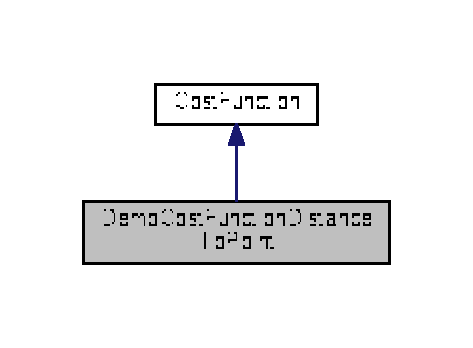
\includegraphics[width=227pt]{classDmpBbo_1_1DemoCostFunctionDistanceToPoint__inherit__graph}
\end{center}
\end{figure}


Collaboration diagram for Demo\+Cost\+Function\+Distance\+To\+Point\+:
\nopagebreak
\begin{figure}[H]
\begin{center}
\leavevmode
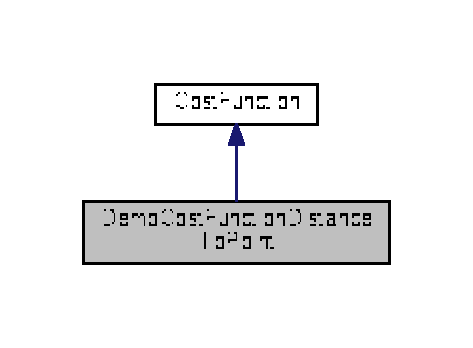
\includegraphics[width=227pt]{classDmpBbo_1_1DemoCostFunctionDistanceToPoint__coll__graph}
\end{center}
\end{figure}
\subsubsection*{Public Member Functions}
\begin{DoxyCompactItemize}
\item 
\hyperlink{classDmpBbo_1_1DemoCostFunctionDistanceToPoint_a6d89a9e9f151cbac696edf37087b9aa2}{Demo\+Cost\+Function\+Distance\+To\+Point} (const Vector\+Xd \&point)
\begin{DoxyCompactList}\small\item\em Constructor. \end{DoxyCompactList}\item 
void \hyperlink{classDmpBbo_1_1DemoCostFunctionDistanceToPoint_a52da51bc9ad0d5f5c8ddd8ca79235ac9}{evaluate} (const Matrix\+Xd \&samples, Vector\+Xd \&costs) const 
\begin{DoxyCompactList}\small\item\em The cost function which defines the cost\+\_\+function. \end{DoxyCompactList}\item 
string \hyperlink{classDmpBbo_1_1DemoCostFunctionDistanceToPoint_a1aca816b42cf0d36118be0ab91120d77}{to\+String} (void) const 
\begin{DoxyCompactList}\small\item\em Returns a string representation of the object. \end{DoxyCompactList}\end{DoxyCompactItemize}


\subsubsection{Detailed Description}
\hyperlink{classDmpBbo_1_1CostFunction}{Cost\+Function} in which the distance to a pre-\/defined point must be minimized. 

Definition at line 54 of file demo\+Evolutionary\+Optimization.\+cpp.



\subsubsection{Constructor \& Destructor Documentation}
\hypertarget{classDmpBbo_1_1DemoCostFunctionDistanceToPoint_a6d89a9e9f151cbac696edf37087b9aa2}{\index{Dmp\+Bbo\+::\+Demo\+Cost\+Function\+Distance\+To\+Point@{Dmp\+Bbo\+::\+Demo\+Cost\+Function\+Distance\+To\+Point}!Demo\+Cost\+Function\+Distance\+To\+Point@{Demo\+Cost\+Function\+Distance\+To\+Point}}
\index{Demo\+Cost\+Function\+Distance\+To\+Point@{Demo\+Cost\+Function\+Distance\+To\+Point}!Dmp\+Bbo\+::\+Demo\+Cost\+Function\+Distance\+To\+Point@{Dmp\+Bbo\+::\+Demo\+Cost\+Function\+Distance\+To\+Point}}
\paragraph[{Demo\+Cost\+Function\+Distance\+To\+Point}]{\setlength{\rightskip}{0pt plus 5cm}{\bf Demo\+Cost\+Function\+Distance\+To\+Point} (
\begin{DoxyParamCaption}
\item[{const Vector\+Xd \&}]{point}
\end{DoxyParamCaption}
)\hspace{0.3cm}{\ttfamily [inline]}}}\label{classDmpBbo_1_1DemoCostFunctionDistanceToPoint_a6d89a9e9f151cbac696edf37087b9aa2}


Constructor. 


\begin{DoxyParams}[1]{Parameters}
\mbox{\tt in}  & {\em point} & Point to which distance must be minimized. \\
\hline
\end{DoxyParams}


Definition at line 60 of file demo\+Evolutionary\+Optimization.\+cpp.


\begin{DoxyCode}
61   \{
62     point\_ = point;
63   \}
\end{DoxyCode}


\subsubsection{Member Function Documentation}
\hypertarget{classDmpBbo_1_1DemoCostFunctionDistanceToPoint_a52da51bc9ad0d5f5c8ddd8ca79235ac9}{\index{Dmp\+Bbo\+::\+Demo\+Cost\+Function\+Distance\+To\+Point@{Dmp\+Bbo\+::\+Demo\+Cost\+Function\+Distance\+To\+Point}!evaluate@{evaluate}}
\index{evaluate@{evaluate}!Dmp\+Bbo\+::\+Demo\+Cost\+Function\+Distance\+To\+Point@{Dmp\+Bbo\+::\+Demo\+Cost\+Function\+Distance\+To\+Point}}
\paragraph[{evaluate}]{\setlength{\rightskip}{0pt plus 5cm}void evaluate (
\begin{DoxyParamCaption}
\item[{const Matrix\+Xd \&}]{samples, }
\item[{Vector\+Xd \&}]{costs}
\end{DoxyParamCaption}
) const\hspace{0.3cm}{\ttfamily [inline]}}}\label{classDmpBbo_1_1DemoCostFunctionDistanceToPoint_a52da51bc9ad0d5f5c8ddd8ca79235ac9}


The cost function which defines the cost\+\_\+function. 


\begin{DoxyParams}[1]{Parameters}
\mbox{\tt in}  & {\em samples} & The samples \\
\hline
\mbox{\tt out}  & {\em costs} & The scalar cost for each sample. \\
\hline
\end{DoxyParams}


Definition at line 70 of file demo\+Evolutionary\+Optimization.\+cpp.


\begin{DoxyCode}
70                                                                 \{
71 \textcolor{preprocessor}{#ifndef NDEBUG // Variables below are only required for asserts; check for NDEBUG to avoid warnings.}
72     \textcolor{keywordtype}{int} n\_dims    = samples.cols();
73 \textcolor{preprocessor}{#endif}
74     assert(n\_dims==point\_.size());
75     
76     \textcolor{keywordtype}{int} n\_samples = samples.rows();
77 
78     costs.resize(n\_samples);
79     \textcolor{keywordflow}{for} (\textcolor{keywordtype}{int} ss=0; ss<n\_samples; ss++)
80     \{
81       \textcolor{comment}{// Cost is distance to point}
82       costs[ss] = sqrt((samples.row(ss) - point\_.transpose()).array().pow(2).sum());
83     \}
84   \}
\end{DoxyCode}
\hypertarget{classDmpBbo_1_1DemoCostFunctionDistanceToPoint_a1aca816b42cf0d36118be0ab91120d77}{\index{Dmp\+Bbo\+::\+Demo\+Cost\+Function\+Distance\+To\+Point@{Dmp\+Bbo\+::\+Demo\+Cost\+Function\+Distance\+To\+Point}!to\+String@{to\+String}}
\index{to\+String@{to\+String}!Dmp\+Bbo\+::\+Demo\+Cost\+Function\+Distance\+To\+Point@{Dmp\+Bbo\+::\+Demo\+Cost\+Function\+Distance\+To\+Point}}
\paragraph[{to\+String}]{\setlength{\rightskip}{0pt plus 5cm}string to\+String (
\begin{DoxyParamCaption}
\item[{void}]{}
\end{DoxyParamCaption}
) const\hspace{0.3cm}{\ttfamily [inline]}, {\ttfamily [virtual]}}}\label{classDmpBbo_1_1DemoCostFunctionDistanceToPoint_a1aca816b42cf0d36118be0ab91120d77}


Returns a string representation of the object. 

\begin{DoxyReturn}{Returns}
A string representation of the object. 
\end{DoxyReturn}


Implements \hyperlink{classDmpBbo_1_1CostFunction_af084bff2ddd6233e9a898faa23f6195c}{Cost\+Function}.



Definition at line 89 of file demo\+Evolutionary\+Optimization.\+cpp.


\begin{DoxyCode}
89                               \{
90     \textcolor{keywordtype}{string} str = \textcolor{stringliteral}{"CostFunctionDistanceToPoint"};
91     \textcolor{keywordflow}{return} str;
92   \}
\end{DoxyCode}


The documentation for this class was generated from the following file\+:\begin{DoxyCompactItemize}
\item 
\hyperlink{demoEvolutionaryOptimization_8cpp}{demo\+Evolutionary\+Optimization.\+cpp}\end{DoxyCompactItemize}

\hypertarget{classDemoTaskApproximateQuadraticFunction}{\subsection{Demo\+Task\+Approximate\+Quadratic\+Function Class Reference}
\label{classDemoTaskApproximateQuadraticFunction}\index{Demo\+Task\+Approximate\+Quadratic\+Function@{Demo\+Task\+Approximate\+Quadratic\+Function}}
}


The task is to choose the parameters a and c such that the function $ y = a*x^2 + c $ best matches a set of target values y\+\_\+target for a set of input values x.  




Inheritance diagram for Demo\+Task\+Approximate\+Quadratic\+Function\+:
\nopagebreak
\begin{figure}[H]
\begin{center}
\leavevmode
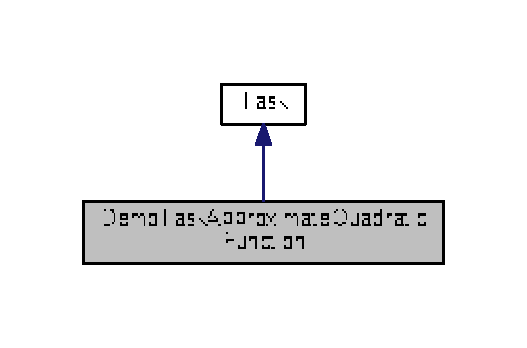
\includegraphics[width=253pt]{classDemoTaskApproximateQuadraticFunction__inherit__graph}
\end{center}
\end{figure}


Collaboration diagram for Demo\+Task\+Approximate\+Quadratic\+Function\+:
\nopagebreak
\begin{figure}[H]
\begin{center}
\leavevmode
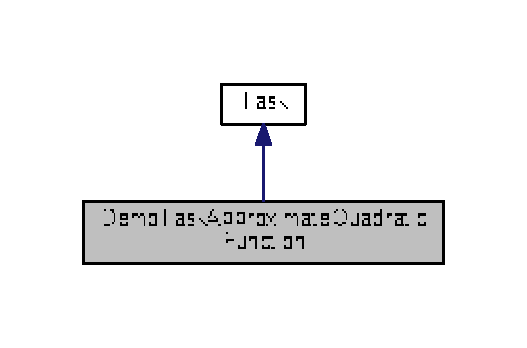
\includegraphics[width=253pt]{classDemoTaskApproximateQuadraticFunction__coll__graph}
\end{center}
\end{figure}
\subsubsection*{Public Member Functions}
\begin{DoxyCompactItemize}
\item 
\hyperlink{classDemoTaskApproximateQuadraticFunction_ac81f6a65537026fd59d52478253e1661}{Demo\+Task\+Approximate\+Quadratic\+Function} (double a, double c, const Vector\+Xd \&inputs)
\begin{DoxyCompactList}\small\item\em Constructor. \end{DoxyCompactList}\item 
void \hyperlink{classDemoTaskApproximateQuadraticFunction_a0f2698f5da124e2a2df8e5894b42d612}{evaluate} (const Matrix\+Xd \&cost\+\_\+vars, const Matrix\+Xd \&task\+\_\+parameters, Vector\+Xd \&costs) const 
\begin{DoxyCompactList}\small\item\em Cost function. \end{DoxyCompactList}\item 
bool \hyperlink{classDemoTaskApproximateQuadraticFunction_a7ae605c4456b382c9d4ecccc1379213d}{save\+Perform\+Rollouts\+Plot\+Script} (string directory) const 
\begin{DoxyCompactList}\small\item\em Save a python script that is able to visualize the rollouts, given the cost-\/relevant variables stored in a file. \end{DoxyCompactList}\item 
string \hyperlink{classDemoTaskApproximateQuadraticFunction_a1aca816b42cf0d36118be0ab91120d77}{to\+String} (void) const 
\begin{DoxyCompactList}\small\item\em Returns a string representation of the object. \end{DoxyCompactList}\end{DoxyCompactItemize}


\subsubsection{Detailed Description}
The task is to choose the parameters a and c such that the function $ y = a*x^2 + c $ best matches a set of target values y\+\_\+target for a set of input values x. 

Definition at line 60 of file demo\+Evolutionary\+Optimization\+Task.\+cpp.



\subsubsection{Constructor \& Destructor Documentation}
\hypertarget{classDemoTaskApproximateQuadraticFunction_ac81f6a65537026fd59d52478253e1661}{\index{Demo\+Task\+Approximate\+Quadratic\+Function@{Demo\+Task\+Approximate\+Quadratic\+Function}!Demo\+Task\+Approximate\+Quadratic\+Function@{Demo\+Task\+Approximate\+Quadratic\+Function}}
\index{Demo\+Task\+Approximate\+Quadratic\+Function@{Demo\+Task\+Approximate\+Quadratic\+Function}!Demo\+Task\+Approximate\+Quadratic\+Function@{Demo\+Task\+Approximate\+Quadratic\+Function}}
\paragraph[{Demo\+Task\+Approximate\+Quadratic\+Function}]{\setlength{\rightskip}{0pt plus 5cm}{\bf Demo\+Task\+Approximate\+Quadratic\+Function} (
\begin{DoxyParamCaption}
\item[{double}]{a, }
\item[{double}]{c, }
\item[{const Vector\+Xd \&}]{inputs}
\end{DoxyParamCaption}
)\hspace{0.3cm}{\ttfamily [inline]}}}\label{classDemoTaskApproximateQuadraticFunction_ac81f6a65537026fd59d52478253e1661}


Constructor. 


\begin{DoxyParams}[1]{Parameters}
\mbox{\tt in}  & {\em a} & a in $ y = a*x^2 + c $ \\
\hline
\mbox{\tt in}  & {\em c} & c in $ y = a*x^2 + c $ \\
\hline
\mbox{\tt in}  & {\em inputs} & x in $ y = a*x^2 + c $ \\
\hline
\end{DoxyParams}


Definition at line 68 of file demo\+Evolutionary\+Optimization\+Task.\+cpp.


\begin{DoxyCode}
69   \{
70     inputs\_ = inputs;
71     \hyperlink{demoEvolutionaryOptimizationTask_8cpp_a8dd69e1c4b8036ab6c2b6f386fe5b6bc}{targetFunction}(a,c,inputs\_,targets\_);
72   \}
\end{DoxyCode}


Here is the call graph for this function\+:
\nopagebreak
\begin{figure}[H]
\begin{center}
\leavevmode
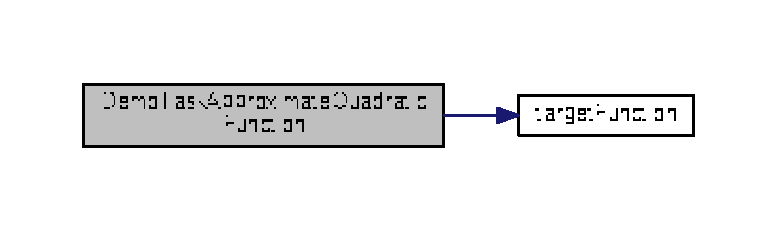
\includegraphics[width=350pt]{classDemoTaskApproximateQuadraticFunction_ac81f6a65537026fd59d52478253e1661_cgraph}
\end{center}
\end{figure}




\subsubsection{Member Function Documentation}
\hypertarget{classDemoTaskApproximateQuadraticFunction_a0f2698f5da124e2a2df8e5894b42d612}{\index{Demo\+Task\+Approximate\+Quadratic\+Function@{Demo\+Task\+Approximate\+Quadratic\+Function}!evaluate@{evaluate}}
\index{evaluate@{evaluate}!Demo\+Task\+Approximate\+Quadratic\+Function@{Demo\+Task\+Approximate\+Quadratic\+Function}}
\paragraph[{evaluate}]{\setlength{\rightskip}{0pt plus 5cm}void evaluate (
\begin{DoxyParamCaption}
\item[{const Matrix\+Xd \&}]{cost\+\_\+vars, }
\item[{const Matrix\+Xd \&}]{task\+\_\+parameters, }
\item[{Vector\+Xd \&}]{costs}
\end{DoxyParamCaption}
) const\hspace{0.3cm}{\ttfamily [inline]}}}\label{classDemoTaskApproximateQuadraticFunction_a0f2698f5da124e2a2df8e5894b42d612}


Cost function. 


\begin{DoxyParams}[1]{Parameters}
\mbox{\tt in}  & {\em cost\+\_\+vars} & y in $ y = a*x^2 + c $ \\
\hline
\mbox{\tt in}  & {\em task\+\_\+parameters} & Ignored \\
\hline
\mbox{\tt out}  & {\em costs} & Costs of the cost\+\_\+vars \\
\hline
\end{DoxyParams}


Definition at line 79 of file demo\+Evolutionary\+Optimization\+Task.\+cpp.


\begin{DoxyCode}
80   \{
81     \textcolor{keywordtype}{int} n\_samples = cost\_vars.rows();
82     costs.resize(n\_samples);
83     
84     VectorXd predictions, diff\_square;
85     \textcolor{keywordflow}{for} (\textcolor{keywordtype}{int} k=0; k<n\_samples; k++)
86     \{
87       predictions = cost\_vars.row(k);
88       diff\_square = (predictions.array()-targets\_.array()).square();
89       costs[k] = diff\_square.mean();
90     \}
91   \}
\end{DoxyCode}
\hypertarget{classDemoTaskApproximateQuadraticFunction_a7ae605c4456b382c9d4ecccc1379213d}{\index{Demo\+Task\+Approximate\+Quadratic\+Function@{Demo\+Task\+Approximate\+Quadratic\+Function}!save\+Perform\+Rollouts\+Plot\+Script@{save\+Perform\+Rollouts\+Plot\+Script}}
\index{save\+Perform\+Rollouts\+Plot\+Script@{save\+Perform\+Rollouts\+Plot\+Script}!Demo\+Task\+Approximate\+Quadratic\+Function@{Demo\+Task\+Approximate\+Quadratic\+Function}}
\paragraph[{save\+Perform\+Rollouts\+Plot\+Script}]{\setlength{\rightskip}{0pt plus 5cm}bool save\+Perform\+Rollouts\+Plot\+Script (
\begin{DoxyParamCaption}
\item[{string}]{directory}
\end{DoxyParamCaption}
) const\hspace{0.3cm}{\ttfamily [inline]}}}\label{classDemoTaskApproximateQuadraticFunction_a7ae605c4456b382c9d4ecccc1379213d}


Save a python script that is able to visualize the rollouts, given the cost-\/relevant variables stored in a file. 


\begin{DoxyParams}[1]{Parameters}
\mbox{\tt in}  & {\em directory} & Directory in which to save the python script \\
\hline
\end{DoxyParams}
\begin{DoxyReturn}{Returns}
true if saving the script was successful, false otherwise 
\end{DoxyReturn}


Definition at line 98 of file demo\+Evolutionary\+Optimization\+Task.\+cpp.


\begin{DoxyCode}
99   \{
100     \textcolor{keywordtype}{string} filename = directory + \textcolor{stringliteral}{"/plotRollouts.py"};
101     
102     std::ofstream file;
103     file.open(filename.c\_str());
104     \textcolor{keywordflow}{if} (!file.is\_open())
105     \{
106       std::cerr << \textcolor{stringliteral}{"Couldn't open file '"} << filename << \textcolor{stringliteral}{"' for writing."} << std::endl;
107       \textcolor{keywordflow}{return} \textcolor{keyword}{false};
108     \}
109     
110     
111     file << \textcolor{stringliteral}{"import numpy as np"} << endl;
112     file << \textcolor{stringliteral}{"import matplotlib.pyplot as plt"} << endl;
113     file << \textcolor{stringliteral}{"import sys, os"} << endl;
114     file << \textcolor{stringliteral}{"def plotRollouts(cost\_vars,ax):"} << endl;
115     file << \textcolor{stringliteral}{"    inputs = ["};
116     file << fixed;
117     \textcolor{keywordflow}{for} (\textcolor{keywordtype}{int} ii=0; ii<inputs\_.size(); ii++)
118     \{
119       \textcolor{keywordflow}{if} (ii>0) file << \textcolor{stringliteral}{", "};
120       file << inputs\_[ii];
121     \}
122     file << \textcolor{stringliteral}{"]"} << endl;
123     file << \textcolor{stringliteral}{"    targets = ["};
124     \textcolor{keywordflow}{for} (\textcolor{keywordtype}{int} ii=0; ii<targets\_.size(); ii++)
125     \{
126       \textcolor{keywordflow}{if} (ii>0) file << \textcolor{stringliteral}{", "};
127       file << targets\_[ii];
128     \}
129     file << \textcolor{stringliteral}{"]"} << endl;
130     file << \textcolor{stringliteral}{"    line\_handles = ax.plot(inputs,cost\_vars.T,linewidth=0.5)"} << endl;
131     file << \textcolor{stringliteral}{"    ax.plot(inputs,targets,'-o',color='k',linewidth=2)"} << endl;
132     file << \textcolor{stringliteral}{"    return line\_handles"} << endl;
133     file << \textcolor{stringliteral}{"if \_\_name\_\_=='\_\_main\_\_':"} << endl;
134     file << \textcolor{stringliteral}{"    # See if input directory was passed"} << endl;
135     file << \textcolor{stringliteral}{"    if (len(sys.argv)==2):"} << endl;
136     file << \textcolor{stringliteral}{"      directory = str(sys.argv[1])"} << endl;
137     file << \textcolor{stringliteral}{"    else:"} << endl;
138     file << \textcolor{stringliteral}{"      print 'Usage: '+sys.argv[0]+' <directory>';"} << endl;
139     file << \textcolor{stringliteral}{"      sys.exit()"} << endl;
140     file << \textcolor{stringliteral}{"    cost\_vars = np.loadtxt(directory+\(\backslash\)"cost\_vars.txt\(\backslash\)")"} << endl;
141     file << \textcolor{stringliteral}{"    fig = plt.figure()"} << endl;
142     file << \textcolor{stringliteral}{"    ax = fig.gca()"} << endl;
143     file << \textcolor{stringliteral}{"    plotRollouts(cost\_vars,ax)"} << endl;
144     file << \textcolor{stringliteral}{"    plt.show()"} << endl;
145     
146     file.close();
147     
148     \textcolor{keywordflow}{return} \textcolor{keyword}{true};
149   \}
\end{DoxyCode}
\hypertarget{classDemoTaskApproximateQuadraticFunction_a1aca816b42cf0d36118be0ab91120d77}{\index{Demo\+Task\+Approximate\+Quadratic\+Function@{Demo\+Task\+Approximate\+Quadratic\+Function}!to\+String@{to\+String}}
\index{to\+String@{to\+String}!Demo\+Task\+Approximate\+Quadratic\+Function@{Demo\+Task\+Approximate\+Quadratic\+Function}}
\paragraph[{to\+String}]{\setlength{\rightskip}{0pt plus 5cm}string to\+String (
\begin{DoxyParamCaption}
\item[{void}]{}
\end{DoxyParamCaption}
) const\hspace{0.3cm}{\ttfamily [inline]}, {\ttfamily [virtual]}}}\label{classDemoTaskApproximateQuadraticFunction_a1aca816b42cf0d36118be0ab91120d77}


Returns a string representation of the object. 

\begin{DoxyReturn}{Returns}
A string representation of the object. 
\end{DoxyReturn}


Implements \hyperlink{classDmpBbo_1_1Task_af084bff2ddd6233e9a898faa23f6195c}{Task}.



Definition at line 154 of file demo\+Evolutionary\+Optimization\+Task.\+cpp.


\begin{DoxyCode}
155   \{
156     \textcolor{keywordtype}{string} str = \textcolor{stringliteral}{"TaskApproximateQuadraticFunctionSolver"};
157     \textcolor{keywordflow}{return} str;
158   \}
\end{DoxyCode}


The documentation for this class was generated from the following file\+:\begin{DoxyCompactItemize}
\item 
\hyperlink{demoEvolutionaryOptimizationTask_8cpp}{demo\+Evolutionary\+Optimization\+Task.\+cpp}\end{DoxyCompactItemize}

\hypertarget{classDemoTaskSolverApproximateQuadraticFunction}{\subsection{Demo\+Task\+Solver\+Approximate\+Quadratic\+Function Class Reference}
\label{classDemoTaskSolverApproximateQuadraticFunction}\index{Demo\+Task\+Solver\+Approximate\+Quadratic\+Function@{Demo\+Task\+Solver\+Approximate\+Quadratic\+Function}}
}


The task solver tunes the parameters a and c such that the function $ y = a*x^2 + c $ best matches a set of target values y\+\_\+target for a set of input values x.  




Inheritance diagram for Demo\+Task\+Solver\+Approximate\+Quadratic\+Function\+:
\nopagebreak
\begin{figure}[H]
\begin{center}
\leavevmode
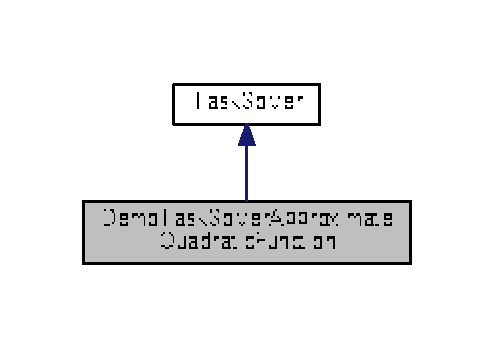
\includegraphics[width=237pt]{classDemoTaskSolverApproximateQuadraticFunction__inherit__graph}
\end{center}
\end{figure}


Collaboration diagram for Demo\+Task\+Solver\+Approximate\+Quadratic\+Function\+:
\nopagebreak
\begin{figure}[H]
\begin{center}
\leavevmode
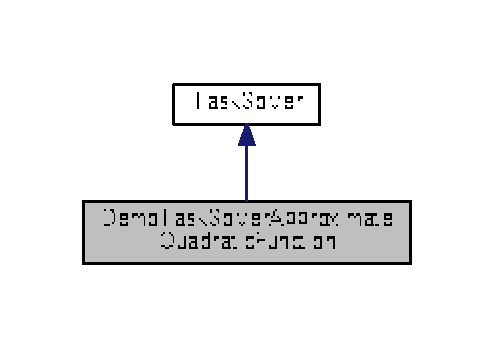
\includegraphics[width=237pt]{classDemoTaskSolverApproximateQuadraticFunction__coll__graph}
\end{center}
\end{figure}
\subsubsection*{Public Member Functions}
\begin{DoxyCompactItemize}
\item 
\hyperlink{classDemoTaskSolverApproximateQuadraticFunction_ae4813da940a633221713aba3a12615c3}{Demo\+Task\+Solver\+Approximate\+Quadratic\+Function} (const Vector\+Xd \&inputs)
\item 
void \hyperlink{classDemoTaskSolverApproximateQuadraticFunction_a51858a828b9e28eb72c39cc0bd212217}{perform\+Rollouts} (const Matrix\+Xd \&samples, const Matrix\+Xd \&task\+\_\+parameters, Matrix\+Xd \&cost\+\_\+vars) const 
\begin{DoxyCompactList}\small\item\em Cost function. \end{DoxyCompactList}\item 
string \hyperlink{classDemoTaskSolverApproximateQuadraticFunction_a1aca816b42cf0d36118be0ab91120d77}{to\+String} (void) const 
\begin{DoxyCompactList}\small\item\em Returns a string representation of the object. \end{DoxyCompactList}\end{DoxyCompactItemize}


\subsubsection{Detailed Description}
The task solver tunes the parameters a and c such that the function $ y = a*x^2 + c $ best matches a set of target values y\+\_\+target for a set of input values x. 

Definition at line 168 of file demo\+Evolutionary\+Optimization\+Task.\+cpp.



\subsubsection{Constructor \& Destructor Documentation}
\hypertarget{classDemoTaskSolverApproximateQuadraticFunction_ae4813da940a633221713aba3a12615c3}{\index{Demo\+Task\+Solver\+Approximate\+Quadratic\+Function@{Demo\+Task\+Solver\+Approximate\+Quadratic\+Function}!Demo\+Task\+Solver\+Approximate\+Quadratic\+Function@{Demo\+Task\+Solver\+Approximate\+Quadratic\+Function}}
\index{Demo\+Task\+Solver\+Approximate\+Quadratic\+Function@{Demo\+Task\+Solver\+Approximate\+Quadratic\+Function}!Demo\+Task\+Solver\+Approximate\+Quadratic\+Function@{Demo\+Task\+Solver\+Approximate\+Quadratic\+Function}}
\paragraph[{Demo\+Task\+Solver\+Approximate\+Quadratic\+Function}]{\setlength{\rightskip}{0pt plus 5cm}{\bf Demo\+Task\+Solver\+Approximate\+Quadratic\+Function} (
\begin{DoxyParamCaption}
\item[{const Vector\+Xd \&}]{inputs}
\end{DoxyParamCaption}
)\hspace{0.3cm}{\ttfamily [inline]}}}\label{classDemoTaskSolverApproximateQuadraticFunction_ae4813da940a633221713aba3a12615c3}

\begin{DoxyParams}[1]{Parameters}
\mbox{\tt in}  & {\em inputs} & x in $ y = a*x^2 + c $ \\
\hline
\end{DoxyParams}


Definition at line 174 of file demo\+Evolutionary\+Optimization\+Task.\+cpp.


\begin{DoxyCode}
175   \{
176     inputs\_ = inputs;
177   \}
\end{DoxyCode}


\subsubsection{Member Function Documentation}
\hypertarget{classDemoTaskSolverApproximateQuadraticFunction_a51858a828b9e28eb72c39cc0bd212217}{\index{Demo\+Task\+Solver\+Approximate\+Quadratic\+Function@{Demo\+Task\+Solver\+Approximate\+Quadratic\+Function}!perform\+Rollouts@{perform\+Rollouts}}
\index{perform\+Rollouts@{perform\+Rollouts}!Demo\+Task\+Solver\+Approximate\+Quadratic\+Function@{Demo\+Task\+Solver\+Approximate\+Quadratic\+Function}}
\paragraph[{perform\+Rollouts}]{\setlength{\rightskip}{0pt plus 5cm}void perform\+Rollouts (
\begin{DoxyParamCaption}
\item[{const Matrix\+Xd \&}]{samples, }
\item[{const Matrix\+Xd \&}]{task\+\_\+parameters, }
\item[{Matrix\+Xd \&}]{cost\+\_\+vars}
\end{DoxyParamCaption}
) const\hspace{0.3cm}{\ttfamily [inline]}}}\label{classDemoTaskSolverApproximateQuadraticFunction_a51858a828b9e28eb72c39cc0bd212217}


Cost function. 


\begin{DoxyParams}[1]{Parameters}
\mbox{\tt in}  & {\em samples} & Samples containing variations of a and c (in $ y = a*x^2 + c $) \\
\hline
\mbox{\tt in}  & {\em task\+\_\+parameters} & Ignored \\
\hline
\mbox{\tt in}  & {\em cost\+\_\+vars} & Cost-\/relevant variables, containing the predictions \\
\hline
\end{DoxyParams}


Definition at line 184 of file demo\+Evolutionary\+Optimization\+Task.\+cpp.


\begin{DoxyCode}
185   \{
186     \textcolor{keywordtype}{int} n\_samples = samples.rows();
187     cost\_vars.resize(n\_samples,inputs\_.size());
188     
189     VectorXd predictions, diff\_square;
190     \textcolor{keywordflow}{for} (\textcolor{keywordtype}{int} k=0; k<n\_samples; k++)
191     \{
192       \textcolor{keywordtype}{double} a = samples(k,0);
193       \textcolor{keywordtype}{double} c = samples(k,1);
194       \hyperlink{demoEvolutionaryOptimizationTask_8cpp_a8dd69e1c4b8036ab6c2b6f386fe5b6bc}{targetFunction}(a,c,inputs\_,predictions);
195       
196       cost\_vars.row(k) = predictions;
197     \}
198   \}
\end{DoxyCode}


Here is the call graph for this function\+:
\nopagebreak
\begin{figure}[H]
\begin{center}
\leavevmode
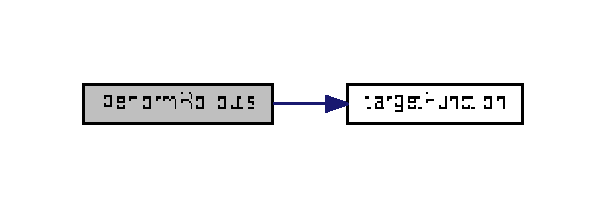
\includegraphics[width=291pt]{classDemoTaskSolverApproximateQuadraticFunction_a51858a828b9e28eb72c39cc0bd212217_cgraph}
\end{center}
\end{figure}


\hypertarget{classDemoTaskSolverApproximateQuadraticFunction_a1aca816b42cf0d36118be0ab91120d77}{\index{Demo\+Task\+Solver\+Approximate\+Quadratic\+Function@{Demo\+Task\+Solver\+Approximate\+Quadratic\+Function}!to\+String@{to\+String}}
\index{to\+String@{to\+String}!Demo\+Task\+Solver\+Approximate\+Quadratic\+Function@{Demo\+Task\+Solver\+Approximate\+Quadratic\+Function}}
\paragraph[{to\+String}]{\setlength{\rightskip}{0pt plus 5cm}string to\+String (
\begin{DoxyParamCaption}
\item[{void}]{}
\end{DoxyParamCaption}
) const\hspace{0.3cm}{\ttfamily [inline]}, {\ttfamily [virtual]}}}\label{classDemoTaskSolverApproximateQuadraticFunction_a1aca816b42cf0d36118be0ab91120d77}


Returns a string representation of the object. 

\begin{DoxyReturn}{Returns}
A string representation of the object. 
\end{DoxyReturn}


Implements \hyperlink{classDmpBbo_1_1TaskSolver_af084bff2ddd6233e9a898faa23f6195c}{Task\+Solver}.



Definition at line 203 of file demo\+Evolutionary\+Optimization\+Task.\+cpp.


\begin{DoxyCode}
204   \{
205     \textcolor{keywordtype}{string} str = \textcolor{stringliteral}{"TaskApproximateQuadraticFunctionSolver"};
206     \textcolor{keywordflow}{return} str;
207   \}
\end{DoxyCode}


The documentation for this class was generated from the following file\+:\begin{DoxyCompactItemize}
\item 
\hyperlink{demoEvolutionaryOptimizationTask_8cpp}{demo\+Evolutionary\+Optimization\+Task.\+cpp}\end{DoxyCompactItemize}

\hypertarget{classDmpBbo_1_1DistributionGaussian}{\subsection{Distribution\+Gaussian Class Reference}
\label{classDmpBbo_1_1DistributionGaussian}\index{Distribution\+Gaussian@{Distribution\+Gaussian}}
}


A class for representing a Gaussian distribution.  




{\ttfamily \#include $<$Distribution\+Gaussian.\+hpp$>$}

\subsubsection*{Public Member Functions}
\begin{DoxyCompactItemize}
\item 
\hyperlink{classDmpBbo_1_1DistributionGaussian_a429296bb71ed97282ef49232431b7b51}{Distribution\+Gaussian} (const Eigen\+::\+Vector\+Xd \&\hyperlink{classDmpBbo_1_1DistributionGaussian_a612f996501aac7e31237a21b47d03d72}{mean}, const Eigen\+::\+Matrix\+Xd \&\hyperlink{classDmpBbo_1_1DistributionGaussian_a5d2adde253815df42d471a876173868c}{covar})
\begin{DoxyCompactList}\small\item\em Construct the Gaussian distribution with a mean and covariance matrix. \end{DoxyCompactList}\item 
void \hyperlink{classDmpBbo_1_1DistributionGaussian_ae5cb5c89a2db5d549f7a2abec2cd58f8}{generate\+Samples} (int n\+\_\+samples, Eigen\+::\+Matrix\+Xd \&samples) const 
\begin{DoxyCompactList}\small\item\em Generate samples from the distribution. \end{DoxyCompactList}\item 
\hyperlink{classDmpBbo_1_1DistributionGaussian}{Distribution\+Gaussian} $\ast$ \hyperlink{classDmpBbo_1_1DistributionGaussian_a507b8f2538f519dd625025b1768f7938}{clone} (void) const 
\begin{DoxyCompactList}\small\item\em Make a deep copy of the object. \end{DoxyCompactList}\item 
const Eigen\+::\+Vector\+Xd \& \hyperlink{classDmpBbo_1_1DistributionGaussian_a612f996501aac7e31237a21b47d03d72}{mean} (void) const 
\begin{DoxyCompactList}\small\item\em Accessor get function for the mean. \end{DoxyCompactList}\item 
const Eigen\+::\+Matrix\+Xd \& \hyperlink{classDmpBbo_1_1DistributionGaussian_a5d2adde253815df42d471a876173868c}{covar} (void) const 
\begin{DoxyCompactList}\small\item\em Accessor get function for the covariance matrix. \end{DoxyCompactList}\item 
void \hyperlink{classDmpBbo_1_1DistributionGaussian_ac9783c093d50c99c387c241b3bc8729d}{set\+\_\+mean} (const Eigen\+::\+Vector\+Xd \&\hyperlink{classDmpBbo_1_1DistributionGaussian_a612f996501aac7e31237a21b47d03d72}{mean})
\begin{DoxyCompactList}\small\item\em Accessor set function for the mean. \end{DoxyCompactList}\item 
void \hyperlink{classDmpBbo_1_1DistributionGaussian_aecae0b0d3ae1d8c47dc4b13d1b24d169}{set\+\_\+covar} (const Eigen\+::\+Matrix\+Xd \&\hyperlink{classDmpBbo_1_1DistributionGaussian_a5d2adde253815df42d471a876173868c}{covar})
\begin{DoxyCompactList}\small\item\em Accessor set function for the covar. \end{DoxyCompactList}\end{DoxyCompactItemize}
\subsubsection*{Friends}
\begin{DoxyCompactItemize}
\item 
class \hyperlink{classDmpBbo_1_1DistributionGaussian_ac98d07dd8f7b70e16ccb9a01abf56b9c}{boost\+::serialization\+::access}
\begin{DoxyCompactList}\small\item\em Give boost serialization access to private members. \end{DoxyCompactList}\item 
std\+::ostream \& \hyperlink{classDmpBbo_1_1DistributionGaussian_a117d84e639d830f86b54aa05ac129c2f}{operator$<$$<$} (std\+::ostream \&output, const \hyperlink{classDmpBbo_1_1DistributionGaussian}{Distribution\+Gaussian} \&distribution)
\begin{DoxyCompactList}\small\item\em Print to output stream. \end{DoxyCompactList}\end{DoxyCompactItemize}


\subsubsection{Detailed Description}
A class for representing a Gaussian distribution. 

This is mainly a wrapper around boost functionality The reason to make the wrapper is to provide functionality for serialization/deserialization. 

Definition at line 44 of file Distribution\+Gaussian.\+hpp.



\subsubsection{Constructor \& Destructor Documentation}
\hypertarget{classDmpBbo_1_1DistributionGaussian_a429296bb71ed97282ef49232431b7b51}{\index{Dmp\+Bbo\+::\+Distribution\+Gaussian@{Dmp\+Bbo\+::\+Distribution\+Gaussian}!Distribution\+Gaussian@{Distribution\+Gaussian}}
\index{Distribution\+Gaussian@{Distribution\+Gaussian}!Dmp\+Bbo\+::\+Distribution\+Gaussian@{Dmp\+Bbo\+::\+Distribution\+Gaussian}}
\paragraph[{Distribution\+Gaussian}]{\setlength{\rightskip}{0pt plus 5cm}{\bf Distribution\+Gaussian} (
\begin{DoxyParamCaption}
\item[{const Eigen\+::\+Vector\+Xd \&}]{mean, }
\item[{const Eigen\+::\+Matrix\+Xd \&}]{covar}
\end{DoxyParamCaption}
)}}\label{classDmpBbo_1_1DistributionGaussian_a429296bb71ed97282ef49232431b7b51}


Construct the Gaussian distribution with a mean and covariance matrix. 


\begin{DoxyParams}[1]{Parameters}
\mbox{\tt in}  & {\em mean} & Mean of the distribution \\
\hline
\mbox{\tt in}  & {\em covar} & Covariance matrix of the distribution \\
\hline
\end{DoxyParams}


Definition at line 54 of file Distribution\+Gaussian.\+cpp.


\begin{DoxyCode}
55 \{
56   mean\_ = \hyperlink{classDmpBbo_1_1DistributionGaussian_a612f996501aac7e31237a21b47d03d72}{mean};
57   \hyperlink{classDmpBbo_1_1DistributionGaussian_aecae0b0d3ae1d8c47dc4b13d1b24d169}{set\_covar}(\hyperlink{classDmpBbo_1_1DistributionGaussian_a5d2adde253815df42d471a876173868c}{covar});
58 \}
\end{DoxyCode}


\subsubsection{Member Function Documentation}
\hypertarget{classDmpBbo_1_1DistributionGaussian_ae5cb5c89a2db5d549f7a2abec2cd58f8}{\index{Dmp\+Bbo\+::\+Distribution\+Gaussian@{Dmp\+Bbo\+::\+Distribution\+Gaussian}!generate\+Samples@{generate\+Samples}}
\index{generate\+Samples@{generate\+Samples}!Dmp\+Bbo\+::\+Distribution\+Gaussian@{Dmp\+Bbo\+::\+Distribution\+Gaussian}}
\paragraph[{generate\+Samples}]{\setlength{\rightskip}{0pt plus 5cm}void generate\+Samples (
\begin{DoxyParamCaption}
\item[{int}]{n\+\_\+samples, }
\item[{Eigen\+::\+Matrix\+Xd \&}]{samples}
\end{DoxyParamCaption}
) const}}\label{classDmpBbo_1_1DistributionGaussian_ae5cb5c89a2db5d549f7a2abec2cd58f8}


Generate samples from the distribution. 


\begin{DoxyParams}[1]{Parameters}
\mbox{\tt in}  & {\em n\+\_\+samples} & Number of samples to sample \\
\hline
\mbox{\tt in}  & {\em samples} & the samples themselves (size n\+\_\+samples X dim(mean) \\
\hline
\end{DoxyParams}


Definition at line 78 of file Distribution\+Gaussian.\+cpp.


\begin{DoxyCode}
79 \{
80   \textcolor{keywordflow}{if} (covar\_decomposed\_.size()==0)
81   \{
82     \textcolor{comment}{// Now perform the Cholesky decomposition, which makes it easier to generate samples. }
83     MatrixXd A(covar\_.llt().matrixL());
84     covar\_decomposed\_ = A;
85     \textcolor{comment}{// Remark: it would have been better to do this in the constructor and set\_covar, }
86     \textcolor{comment}{// but I couldn't get it to work with boost::serialization (I tried hard)}
87   \}
88   
89   
90   \textcolor{keywordtype}{int} n\_dims = mean\_.size();
91   samples.resize(n\_samples,n\_dims);
92   
93   \textcolor{comment}{// http://en.wikipedia.org/wiki/Multivariate\_normal\_distribution#Drawing\_values\_from\_the\_distribution}
94   VectorXd z(n\_dims);
95   \textcolor{keywordflow}{for} (\textcolor{keywordtype}{int} i\_sample=0; i\_sample<n\_samples; i\_sample++)
96   \{
97     \textcolor{comment}{// Generate vector with samples from standard normal distribution N(0,1) }
98     \textcolor{keywordflow}{for} (\textcolor{keywordtype}{int} i\_dim=0; i\_dim<n\_dims; i\_dim++)
99       z(i\_dim) = (*normal\_distribution\_unit)();
100 
101     \textcolor{comment}{// Compute x = mu + Az}
102     samples.row(i\_sample) = mean\_ + covar\_decomposed\_*z;
103   \}  
104 \}
\end{DoxyCode}
\hypertarget{classDmpBbo_1_1DistributionGaussian_a507b8f2538f519dd625025b1768f7938}{\index{Dmp\+Bbo\+::\+Distribution\+Gaussian@{Dmp\+Bbo\+::\+Distribution\+Gaussian}!clone@{clone}}
\index{clone@{clone}!Dmp\+Bbo\+::\+Distribution\+Gaussian@{Dmp\+Bbo\+::\+Distribution\+Gaussian}}
\paragraph[{clone}]{\setlength{\rightskip}{0pt plus 5cm}{\bf Distribution\+Gaussian} $\ast$ clone (
\begin{DoxyParamCaption}
\item[{void}]{}
\end{DoxyParamCaption}
) const}}\label{classDmpBbo_1_1DistributionGaussian_a507b8f2538f519dd625025b1768f7938}


Make a deep copy of the object. 

\begin{DoxyReturn}{Returns}
A deep copy of the object. 
\end{DoxyReturn}


Definition at line 60 of file Distribution\+Gaussian.\+cpp.


\begin{DoxyCode}
61 \{
62   \textcolor{keywordflow}{return} \textcolor{keyword}{new} \hyperlink{classDmpBbo_1_1DistributionGaussian_a429296bb71ed97282ef49232431b7b51}{DistributionGaussian}(\hyperlink{classDmpBbo_1_1DistributionGaussian_a612f996501aac7e31237a21b47d03d72}{mean}(),\hyperlink{classDmpBbo_1_1DistributionGaussian_a5d2adde253815df42d471a876173868c}{covar}()); 
63 \}
\end{DoxyCode}
\hypertarget{classDmpBbo_1_1DistributionGaussian_a612f996501aac7e31237a21b47d03d72}{\index{Dmp\+Bbo\+::\+Distribution\+Gaussian@{Dmp\+Bbo\+::\+Distribution\+Gaussian}!mean@{mean}}
\index{mean@{mean}!Dmp\+Bbo\+::\+Distribution\+Gaussian@{Dmp\+Bbo\+::\+Distribution\+Gaussian}}
\paragraph[{mean}]{\setlength{\rightskip}{0pt plus 5cm}const Eigen\+::\+Vector\+Xd\& mean (
\begin{DoxyParamCaption}
\item[{void}]{}
\end{DoxyParamCaption}
) const\hspace{0.3cm}{\ttfamily [inline]}}}\label{classDmpBbo_1_1DistributionGaussian_a612f996501aac7e31237a21b47d03d72}


Accessor get function for the mean. 

\begin{DoxyReturn}{Returns}
The mean of the distribution 
\end{DoxyReturn}


Definition at line 68 of file Distribution\+Gaussian.\+hpp.


\begin{DoxyCode}
68 \{ \textcolor{keywordflow}{return} mean\_;   \}
\end{DoxyCode}
\hypertarget{classDmpBbo_1_1DistributionGaussian_a5d2adde253815df42d471a876173868c}{\index{Dmp\+Bbo\+::\+Distribution\+Gaussian@{Dmp\+Bbo\+::\+Distribution\+Gaussian}!covar@{covar}}
\index{covar@{covar}!Dmp\+Bbo\+::\+Distribution\+Gaussian@{Dmp\+Bbo\+::\+Distribution\+Gaussian}}
\paragraph[{covar}]{\setlength{\rightskip}{0pt plus 5cm}const Eigen\+::\+Matrix\+Xd\& covar (
\begin{DoxyParamCaption}
\item[{void}]{}
\end{DoxyParamCaption}
) const\hspace{0.3cm}{\ttfamily [inline]}}}\label{classDmpBbo_1_1DistributionGaussian_a5d2adde253815df42d471a876173868c}


Accessor get function for the covariance matrix. 

\begin{DoxyReturn}{Returns}
The covariance matrix of the distribution 
\end{DoxyReturn}


Definition at line 74 of file Distribution\+Gaussian.\+hpp.


\begin{DoxyCode}
74 \{ \textcolor{keywordflow}{return} covar\_; \}
\end{DoxyCode}
\hypertarget{classDmpBbo_1_1DistributionGaussian_ac9783c093d50c99c387c241b3bc8729d}{\index{Dmp\+Bbo\+::\+Distribution\+Gaussian@{Dmp\+Bbo\+::\+Distribution\+Gaussian}!set\+\_\+mean@{set\+\_\+mean}}
\index{set\+\_\+mean@{set\+\_\+mean}!Dmp\+Bbo\+::\+Distribution\+Gaussian@{Dmp\+Bbo\+::\+Distribution\+Gaussian}}
\paragraph[{set\+\_\+mean}]{\setlength{\rightskip}{0pt plus 5cm}void set\+\_\+mean (
\begin{DoxyParamCaption}
\item[{const Eigen\+::\+Vector\+Xd \&}]{mean}
\end{DoxyParamCaption}
)}}\label{classDmpBbo_1_1DistributionGaussian_ac9783c093d50c99c387c241b3bc8729d}


Accessor set function for the mean. 


\begin{DoxyParams}[1]{Parameters}
\mbox{\tt in}  & {\em mean} & The new mean of the distribution \\
\hline
\end{DoxyParams}


Definition at line 65 of file Distribution\+Gaussian.\+cpp.


\begin{DoxyCode}
65                                                         \{ 
66   assert(\hyperlink{classDmpBbo_1_1DistributionGaussian_a612f996501aac7e31237a21b47d03d72}{mean}.size()==mean\_.size());  
67   mean\_ = \hyperlink{classDmpBbo_1_1DistributionGaussian_a612f996501aac7e31237a21b47d03d72}{mean};
68 \}
\end{DoxyCode}
\hypertarget{classDmpBbo_1_1DistributionGaussian_aecae0b0d3ae1d8c47dc4b13d1b24d169}{\index{Dmp\+Bbo\+::\+Distribution\+Gaussian@{Dmp\+Bbo\+::\+Distribution\+Gaussian}!set\+\_\+covar@{set\+\_\+covar}}
\index{set\+\_\+covar@{set\+\_\+covar}!Dmp\+Bbo\+::\+Distribution\+Gaussian@{Dmp\+Bbo\+::\+Distribution\+Gaussian}}
\paragraph[{set\+\_\+covar}]{\setlength{\rightskip}{0pt plus 5cm}void set\+\_\+covar (
\begin{DoxyParamCaption}
\item[{const Eigen\+::\+Matrix\+Xd \&}]{covar}
\end{DoxyParamCaption}
)}}\label{classDmpBbo_1_1DistributionGaussian_aecae0b0d3ae1d8c47dc4b13d1b24d169}


Accessor set function for the covar. 


\begin{DoxyParams}[1]{Parameters}
\mbox{\tt in}  & {\em covar} & The new covariance matrix of the distribution \\
\hline
\end{DoxyParams}


Definition at line 71 of file Distribution\+Gaussian.\+cpp.


\begin{DoxyCode}
71                                                           \{ 
72   assert(\hyperlink{classDmpBbo_1_1DistributionGaussian_a5d2adde253815df42d471a876173868c}{covar}.cols()==\hyperlink{classDmpBbo_1_1DistributionGaussian_a5d2adde253815df42d471a876173868c}{covar}.rows());
73   assert(\hyperlink{classDmpBbo_1_1DistributionGaussian_a5d2adde253815df42d471a876173868c}{covar}.rows()==mean\_.size());
74   covar\_ = \hyperlink{classDmpBbo_1_1DistributionGaussian_a5d2adde253815df42d471a876173868c}{covar};
75   covar\_decomposed\_ = MatrixXd::Zero(0,0);
76 \}
\end{DoxyCode}


\subsubsection{Friends And Related Function Documentation}
\hypertarget{classDmpBbo_1_1DistributionGaussian_ac98d07dd8f7b70e16ccb9a01abf56b9c}{\index{Dmp\+Bbo\+::\+Distribution\+Gaussian@{Dmp\+Bbo\+::\+Distribution\+Gaussian}!boost\+::serialization\+::access@{boost\+::serialization\+::access}}
\index{boost\+::serialization\+::access@{boost\+::serialization\+::access}!Dmp\+Bbo\+::\+Distribution\+Gaussian@{Dmp\+Bbo\+::\+Distribution\+Gaussian}}
\paragraph[{boost\+::serialization\+::access}]{\setlength{\rightskip}{0pt plus 5cm}friend class boost\+::serialization\+::access\hspace{0.3cm}{\ttfamily [friend]}}}\label{classDmpBbo_1_1DistributionGaussian_ac98d07dd8f7b70e16ccb9a01abf56b9c}


Give boost serialization access to private members. 



Definition at line 111 of file Distribution\+Gaussian.\+hpp.

\hypertarget{classDmpBbo_1_1DistributionGaussian_a117d84e639d830f86b54aa05ac129c2f}{\index{Dmp\+Bbo\+::\+Distribution\+Gaussian@{Dmp\+Bbo\+::\+Distribution\+Gaussian}!operator$<$$<$@{operator$<$$<$}}
\index{operator$<$$<$@{operator$<$$<$}!Dmp\+Bbo\+::\+Distribution\+Gaussian@{Dmp\+Bbo\+::\+Distribution\+Gaussian}}
\paragraph[{operator$<$$<$}]{\setlength{\rightskip}{0pt plus 5cm}std\+::ostream\& operator$<$$<$ (
\begin{DoxyParamCaption}
\item[{std\+::ostream \&}]{output, }
\item[{const {\bf Distribution\+Gaussian} \&}]{distribution}
\end{DoxyParamCaption}
)\hspace{0.3cm}{\ttfamily [friend]}}}\label{classDmpBbo_1_1DistributionGaussian_a117d84e639d830f86b54aa05ac129c2f}


Print to output stream. 


\begin{DoxyParams}[1]{Parameters}
\mbox{\tt in}  & {\em output} & Output stream to which to write to \\
\hline
\mbox{\tt in}  & {\em distribution} & Distribution to write \\
\hline
\end{DoxyParams}
\begin{DoxyReturn}{Returns}
Output stream 
\end{DoxyReturn}


Definition at line 107 of file Distribution\+Gaussian.\+cpp.


\begin{DoxyCode}
108 \{
109   output << \textcolor{stringliteral}{"N(["} << toString(distribution.mean\_) << \textcolor{stringliteral}{"], ["}<< toString(distribution.covar\_) << \textcolor{stringliteral}{"])"};
110   \textcolor{keywordflow}{return} output;
111 \}
\end{DoxyCode}


The documentation for this class was generated from the following files\+:\begin{DoxyCompactItemize}
\item 
\hyperlink{DistributionGaussian_8hpp}{Distribution\+Gaussian.\+hpp}\item 
\hyperlink{DistributionGaussian_8cpp}{Distribution\+Gaussian.\+cpp}\end{DoxyCompactItemize}

\hypertarget{classDmpBbo_1_1Dmp}{\subsection{Dmp Class Reference}
\label{classDmpBbo_1_1Dmp}\index{Dmp@{Dmp}}
}


Implementation of Dynamical Movement Primitives.  




{\ttfamily \#include $<$Dmp.\+hpp$>$}



Inheritance diagram for Dmp\+:
\nopagebreak
\begin{figure}[H]
\begin{center}
\leavevmode
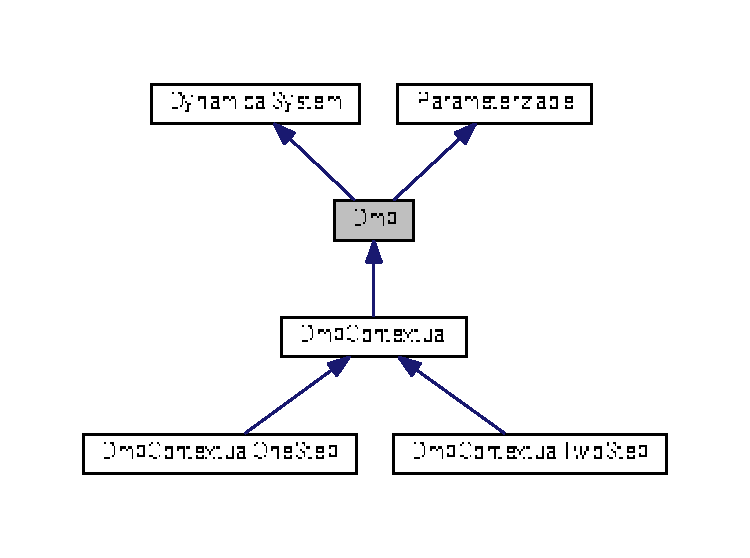
\includegraphics[width=350pt]{classDmpBbo_1_1Dmp__inherit__graph}
\end{center}
\end{figure}


Collaboration diagram for Dmp\+:
\nopagebreak
\begin{figure}[H]
\begin{center}
\leavevmode
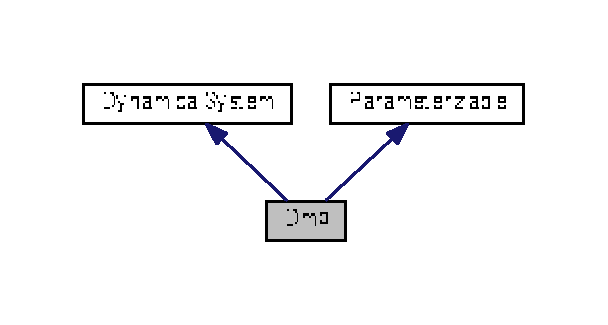
\includegraphics[width=292pt]{classDmpBbo_1_1Dmp__coll__graph}
\end{center}
\end{figure}
\subsubsection*{Public Types}
\begin{DoxyCompactItemize}
\item 
enum \hyperlink{group__Dmps_gaccba8d09ec99ae66e469b3511bb232a4}{Dmp\+Type} \{ {\bfseries I\+J\+S\+P\+E\+E\+R\+T\+\_\+2002\+\_\+\+M\+O\+V\+E\+M\+E\+N\+T}, 
{\bfseries K\+U\+L\+V\+I\+C\+I\+U\+S\+\_\+2012\+\_\+\+J\+O\+I\+N\+I\+N\+G}, 
{\bfseries C\+O\+U\+N\+T\+D\+O\+W\+N\+\_\+2013}
 \}
\begin{DoxyCompactList}\small\item\em Different types of D\+M\+Ps that can be initialized. \end{DoxyCompactList}\end{DoxyCompactItemize}
\subsubsection*{Public Member Functions}
\begin{DoxyCompactItemize}
\item 
\hyperlink{classDmpBbo_1_1Dmp_a4d4f5e7b4c2d8085355c228e2f8a9763}{Dmp} (double \hyperlink{group__DynamicalSystems_ga50eec7ad4c9664b5809ace45b22200d5}{tau}, Eigen\+::\+Vector\+Xd y\+\_\+init, Eigen\+::\+Vector\+Xd y\+\_\+attr, std\+::vector$<$ \hyperlink{classDmpBbo_1_1FunctionApproximator}{Function\+Approximator} $\ast$ $>$ function\+\_\+approximators, double alpha\+\_\+spring\+\_\+damper, \hyperlink{classDmpBbo_1_1DynamicalSystem}{Dynamical\+System} $\ast$goal\+\_\+system, \hyperlink{classDmpBbo_1_1DynamicalSystem}{Dynamical\+System} $\ast$phase\+\_\+system, \hyperlink{classDmpBbo_1_1DynamicalSystem}{Dynamical\+System} $\ast$gating\+\_\+system)
\begin{DoxyCompactList}\small\item\em Initialization constructor. \end{DoxyCompactList}\item 
\hyperlink{classDmpBbo_1_1Dmp_a5861ed5fdc3e3472944c592414b4e8cb}{Dmp} (int n\+\_\+dims\+\_\+dmp, std\+::vector$<$ \hyperlink{classDmpBbo_1_1FunctionApproximator}{Function\+Approximator} $\ast$ $>$ function\+\_\+approximators, double alpha\+\_\+spring\+\_\+damper, \hyperlink{classDmpBbo_1_1DynamicalSystem}{Dynamical\+System} $\ast$goal\+\_\+system, \hyperlink{classDmpBbo_1_1DynamicalSystem}{Dynamical\+System} $\ast$phase\+\_\+system, \hyperlink{classDmpBbo_1_1DynamicalSystem}{Dynamical\+System} $\ast$gating\+\_\+system)
\begin{DoxyCompactList}\small\item\em Initialization constructor for Dmps of known dimensionality, but with unknown initial and attractor states. \end{DoxyCompactList}\item 
\hyperlink{classDmpBbo_1_1Dmp_a0a26f231a585e9f7f7f2d2dd571515b7}{Dmp} (double \hyperlink{group__DynamicalSystems_ga50eec7ad4c9664b5809ace45b22200d5}{tau}, Eigen\+::\+Vector\+Xd y\+\_\+init, Eigen\+::\+Vector\+Xd y\+\_\+attr, std\+::vector$<$ \hyperlink{classDmpBbo_1_1FunctionApproximator}{Function\+Approximator} $\ast$ $>$ function\+\_\+approximators, \hyperlink{group__Dmps_gaccba8d09ec99ae66e469b3511bb232a4}{Dmp\+Type} dmp\+\_\+type=K\+U\+L\+V\+I\+C\+I\+U\+S\+\_\+2012\+\_\+\+J\+O\+I\+N\+I\+N\+G)
\begin{DoxyCompactList}\small\item\em Constructor that initializes the D\+M\+P with default dynamical systems. \end{DoxyCompactList}\item 
\hyperlink{classDmpBbo_1_1Dmp_a30a4c3b7f5568b4d3f57e837241c4774}{Dmp} (int n\+\_\+dims\+\_\+dmp, std\+::vector$<$ \hyperlink{classDmpBbo_1_1FunctionApproximator}{Function\+Approximator} $\ast$ $>$ function\+\_\+approximators, \hyperlink{group__Dmps_gaccba8d09ec99ae66e469b3511bb232a4}{Dmp\+Type} dmp\+\_\+type=K\+U\+L\+V\+I\+C\+I\+U\+S\+\_\+2012\+\_\+\+J\+O\+I\+N\+I\+N\+G)
\begin{DoxyCompactList}\small\item\em Initialization constructor for Dmps of known dimensionality, but with unknown initial and attractor states. \end{DoxyCompactList}\item 
\hyperlink{classDmpBbo_1_1Dmp_a9e16b1345896b7f9cdf1158bb3708545}{Dmp} (double \hyperlink{group__DynamicalSystems_ga50eec7ad4c9664b5809ace45b22200d5}{tau}, Eigen\+::\+Vector\+Xd y\+\_\+init, Eigen\+::\+Vector\+Xd y\+\_\+attr, double alpha\+\_\+spring\+\_\+damper, \hyperlink{classDmpBbo_1_1DynamicalSystem}{Dynamical\+System} $\ast$goal\+\_\+system)
\begin{DoxyCompactList}\small\item\em Initialization constructor for Dmps without a forcing term. \end{DoxyCompactList}\item 
\hyperlink{classDmpBbo_1_1Dmp_adcfceacdeee98011a89fa27cc4799daf}{$\sim$\+Dmp} (void)
\begin{DoxyCompactList}\small\item\em Destructor. \end{DoxyCompactList}\item 
\hyperlink{classDmpBbo_1_1Dmp}{Dmp} $\ast$ \hyperlink{classDmpBbo_1_1Dmp_ace8e32350e4feb2c7ea6b5153c7dc606}{clone} (void) const 
\begin{DoxyCompactList}\small\item\em Return a deep copy of this object. \end{DoxyCompactList}\item 
virtual void \hyperlink{classDmpBbo_1_1Dmp_a44dd496535fde494d8465e7603c93db3}{integrate\+Start} (Eigen\+::\+Ref$<$ Eigen\+::\+Vector\+Xd $>$ x, Eigen\+::\+Ref$<$ Eigen\+::\+Vector\+Xd $>$ xd) const 
\begin{DoxyCompactList}\small\item\em Start integrating the system. \end{DoxyCompactList}\item 
void \hyperlink{classDmpBbo_1_1Dmp_ab564468764e7e4dc7c11e2a786e22c19}{differential\+Equation} (const Eigen\+::\+Vector\+Xd \&x, Eigen\+::\+Ref$<$ Eigen\+::\+Vector\+Xd $>$ xd) const 
\begin{DoxyCompactList}\small\item\em The differential equation which defines the system. \end{DoxyCompactList}\item 
void \hyperlink{classDmpBbo_1_1Dmp_ad62585b1e0bab2b9743782e15e01d694}{analytical\+Solution} (const Eigen\+::\+Vector\+Xd \&ts, Eigen\+::\+Matrix\+Xd \&xs, Eigen\+::\+Matrix\+Xd \&xds, Eigen\+::\+Matrix\+Xd \&forcing\+\_\+terms, Eigen\+::\+Matrix\+Xd \&fa\+\_\+output) const 
\begin{DoxyCompactList}\small\item\em Return analytical solution of the system at certain times (and return forcing terms) \end{DoxyCompactList}\item 
void \hyperlink{classDmpBbo_1_1Dmp_a636531b0dea01397d1338b19e0061360}{analytical\+Solution} (const Eigen\+::\+Vector\+Xd \&ts, Eigen\+::\+Matrix\+Xd \&xs, Eigen\+::\+Matrix\+Xd \&xds, Eigen\+::\+Matrix\+Xd \&forcing\+\_\+terms) const 
\begin{DoxyCompactList}\small\item\em Return analytical solution of the system at certain times (and return forcing terms) \end{DoxyCompactList}\item 
void \hyperlink{classDmpBbo_1_1Dmp_ab6600b58b35bc9e66673d16f68e2e919}{analytical\+Solution} (const Eigen\+::\+Vector\+Xd \&ts, Eigen\+::\+Matrix\+Xd \&xs, Eigen\+::\+Matrix\+Xd \&xds) const 
\begin{DoxyCompactList}\small\item\em Return analytical solution of the system at certain times. \end{DoxyCompactList}\item 
void \hyperlink{classDmpBbo_1_1Dmp_a9b6bbda07ecd4fc7b6c9de57e185ab05}{analytical\+Solution} (const Eigen\+::\+Vector\+Xd \&ts, \hyperlink{classDmpBbo_1_1Trajectory}{Trajectory} \&trajectory) const 
\begin{DoxyCompactList}\small\item\em Return analytical solution of the system at certain times. \end{DoxyCompactList}\item 
void \hyperlink{classDmpBbo_1_1Dmp_ae1e5218e7ebfedf7fb2501dc8af2675f}{analytical\+Solution} (const Eigen\+::\+Vector\+Xd \&ts, \hyperlink{classDmpBbo_1_1Trajectory}{Trajectory} \&trajectory, Eigen\+::\+Matrix\+Xd \&forcing\+\_\+terms) const 
\begin{DoxyCompactList}\small\item\em Return analytical solution of the system at certain times. \end{DoxyCompactList}\item 
virtual void \hyperlink{classDmpBbo_1_1Dmp_aa3ad2fc66e8ce09cfa68032a4a5004b9}{states\+As\+Trajectory} (const Eigen\+::\+Matrix\+Xd \&x\+\_\+in, const Eigen\+::\+Matrix\+Xd \&xd\+\_\+in, Eigen\+::\+Matrix\+Xd \&y\+\_\+out, Eigen\+::\+Matrix\+Xd \&yd\+\_\+out, Eigen\+::\+Matrix\+Xd \&ydd\+\_\+out) const 
\begin{DoxyCompactList}\small\item\em Get the output of a D\+M\+P dynamical system as a trajectory. \end{DoxyCompactList}\item 
virtual void \hyperlink{classDmpBbo_1_1Dmp_a0a477ccb2da97d3b6f5255a147a0e07c}{states\+As\+Trajectory} (const Eigen\+::\+Vector\+Xd \&ts, const Eigen\+::\+Matrix\+Xd \&x\+\_\+in, const Eigen\+::\+Matrix\+Xd \&xd\+\_\+in, \hyperlink{classDmpBbo_1_1Trajectory}{Trajectory} \&trajectory) const 
\begin{DoxyCompactList}\small\item\em Get the output of a D\+M\+P dynamical system as a trajectory. \end{DoxyCompactList}\item 
void \hyperlink{classDmpBbo_1_1Dmp_a5d14dedc6736ec5675b4026437b8a597}{train} (const \hyperlink{classDmpBbo_1_1Trajectory}{Trajectory} \&trajectory)
\begin{DoxyCompactList}\small\item\em Train a D\+M\+P with a trajectory. \end{DoxyCompactList}\item 
void \hyperlink{classDmpBbo_1_1Dmp_abca46c9155c3cfbc71d10aabdcf3384c}{train} (const \hyperlink{classDmpBbo_1_1Trajectory}{Trajectory} \&trajectory, std\+::string save\+\_\+directory, bool overwrite=false)
\begin{DoxyCompactList}\small\item\em Train a D\+M\+P with a trajectory, and write results to file. \end{DoxyCompactList}\item 
virtual void \hyperlink{classDmpBbo_1_1Dmp_a17edb45ef62a4ef7f8c78e4f8f68b249}{set\+\_\+tau} (double \hyperlink{group__DynamicalSystems_ga50eec7ad4c9664b5809ace45b22200d5}{tau})
\begin{DoxyCompactList}\small\item\em Accessor function for the time constant. \end{DoxyCompactList}\item 
virtual void \hyperlink{classDmpBbo_1_1Dmp_ad4e11c676c2add8a992db1caf542f0a0}{set\+\_\+initial\+\_\+state} (const Eigen\+::\+Vector\+Xd \&y\+\_\+init)
\begin{DoxyCompactList}\small\item\em Accessor function for the initial state of the system. \end{DoxyCompactList}\item 
virtual void \hyperlink{classDmpBbo_1_1Dmp_a6dccbd077acfd148f528a48a72a4003f}{set\+\_\+attractor\+\_\+state} (const Eigen\+::\+Vector\+Xd \&y\+\_\+attr)
\begin{DoxyCompactList}\small\item\em Accessor function for the attractor state of the system. \end{DoxyCompactList}\item 
void \hyperlink{classDmpBbo_1_1Dmp_a0b6f58851f4a8fc8b433936cff4c3e7e}{set\+\_\+damping\+\_\+coefficient} (double damping\+\_\+coefficient)
\begin{DoxyCompactList}\small\item\em Accessor function for damping coefficient of spring-\/damper system. \end{DoxyCompactList}\item 
void \hyperlink{classDmpBbo_1_1Dmp_a8844968245473d1fedd2a2b632fb074a}{set\+\_\+spring\+\_\+constant} (double spring\+\_\+constant)
\begin{DoxyCompactList}\small\item\em Accessor function for spring constant of spring-\/damper system. \end{DoxyCompactList}\item 
std\+::string \hyperlink{classDmpBbo_1_1Dmp_a1aca816b42cf0d36118be0ab91120d77}{to\+String} (void) const 
\begin{DoxyCompactList}\small\item\em Returns a string representation of the object. \end{DoxyCompactList}\item 
void \hyperlink{classDmpBbo_1_1Dmp_adaae949509cd3b2e6ce58deb841c80a0}{get\+Selectable\+Parameters} (std\+::set$<$ std\+::string $>$ \&selectable\+\_\+values\+\_\+labels) const 
\begin{DoxyCompactList}\small\item\em Return all the names of the parameter types that can be selected. \end{DoxyCompactList}\item 
void \hyperlink{classDmpBbo_1_1Dmp_a8a976b5db2d1809ece10e431816f0f27}{set\+Selected\+Parameters} (const std\+::set$<$ std\+::string $>$ \&selected\+\_\+values\+\_\+labels)
\begin{DoxyCompactList}\small\item\em Determine which subset of parameters is represented in the vector returned by \hyperlink{classDmpBbo_1_1Parameterizable_aab955bec57f074a991b8be31d6ce54ca}{Parameterizable\+::get\+Parameter\+Vector\+Selected}. \end{DoxyCompactList}\item 
int \hyperlink{classDmpBbo_1_1Dmp_ab24d2485b3b795b516f4844f225100eb}{get\+Parameter\+Vector\+All\+Size} (void) const 
\begin{DoxyCompactList}\small\item\em Get the size of the parameter values vector when it contains all available parameter values. \end{DoxyCompactList}\item 
void \hyperlink{classDmpBbo_1_1Dmp_ac44b51e5335f973eed54f100618e5496}{get\+Parameter\+Vector\+All} (Eigen\+::\+Vector\+Xd \&values) const 
\begin{DoxyCompactList}\small\item\em Return a vector that returns all available parameter values. \end{DoxyCompactList}\item 
void \hyperlink{classDmpBbo_1_1Dmp_a9d3c8f22e8237a805af4935a647e5a50}{set\+Parameter\+Vector\+All} (const Eigen\+::\+Vector\+Xd \&values)
\begin{DoxyCompactList}\small\item\em Set all available parameter values with one vector. \end{DoxyCompactList}\item 
void \hyperlink{classDmpBbo_1_1Dmp_a9dba1f93e426e7511630ec1ece4ace17}{get\+Parameter\+Vector\+Mask} (const std\+::set$<$ std\+::string $>$ selected\+\_\+values\+\_\+labels, Eigen\+::\+Vector\+Xi \&selected\+\_\+mask) const 
\begin{DoxyCompactList}\small\item\em Get a mask for selecting parameters. \end{DoxyCompactList}\item 
void \hyperlink{classDmpBbo_1_1Dmp_a9aef6cbf41e55caa12b62cff77cf1fda}{compute\+Function\+Approximator\+Inputs\+And\+Targets} (const \hyperlink{classDmpBbo_1_1Trajectory}{Trajectory} \&trajectory, Eigen\+::\+Vector\+Xd \&fa\+\_\+inputs\+\_\+phase, Eigen\+::\+Matrix\+Xd \&fa\+\_\+targets) const 
\begin{DoxyCompactList}\small\item\em Given a trajectory, compute the inputs and targets for the function approximators. \end{DoxyCompactList}\item 
virtual void \hyperlink{classDmpBbo_1_1Dmp_a89078b732a4579130e24e3bc59c1713c}{compute\+Function\+Approximator\+Output} (const Eigen\+::\+Matrix\+Xd \&phase\+\_\+state, Eigen\+::\+Matrix\+Xd \&fa\+\_\+output) const 
\begin{DoxyCompactList}\small\item\em Compute the outputs of the function approximators. \end{DoxyCompactList}\item 
void \hyperlink{classDmpBbo_1_1Dmp_a6c44c534fd7bb0b6ad87648692e15269}{set\+\_\+perturbation\+\_\+analytical\+\_\+solution} (double perturbation\+\_\+standard\+\_\+deviation)
\begin{DoxyCompactList}\small\item\em Add a perturbation to the forcing term when computing the analytical solution. \end{DoxyCompactList}\end{DoxyCompactItemize}
\subsubsection*{Protected Member Functions}
\begin{DoxyCompactItemize}
\item 
\hyperlink{classDmpBbo_1_1FunctionApproximator}{Function\+Approximator} $\ast$ \hyperlink{classDmpBbo_1_1Dmp_ac428e2dd848c99ddaf517f2dbacdf3ad}{function\+\_\+approximator} (int i\+\_\+dim) const 
\begin{DoxyCompactList}\small\item\em Get a pointer to the function approximator for a certain dimension. \end{DoxyCompactList}\end{DoxyCompactItemize}
\subsubsection*{Friends}
\begin{DoxyCompactItemize}
\item 
class \hyperlink{classDmpBbo_1_1Dmp_ac98d07dd8f7b70e16ccb9a01abf56b9c}{boost\+::serialization\+::access}
\begin{DoxyCompactList}\small\item\em Give boost serialization access to private members. \end{DoxyCompactList}\end{DoxyCompactItemize}


\subsubsection{Detailed Description}
Implementation of Dynamical Movement Primitives. 

Definition at line 53 of file Dmp.\+hpp.



\subsubsection{Constructor \& Destructor Documentation}
\hypertarget{classDmpBbo_1_1Dmp_a4d4f5e7b4c2d8085355c228e2f8a9763}{\index{Dmp\+Bbo\+::\+Dmp@{Dmp\+Bbo\+::\+Dmp}!Dmp@{Dmp}}
\index{Dmp@{Dmp}!Dmp\+Bbo\+::\+Dmp@{Dmp\+Bbo\+::\+Dmp}}
\paragraph[{Dmp}]{\setlength{\rightskip}{0pt plus 5cm}{\bf Dmp} (
\begin{DoxyParamCaption}
\item[{double}]{tau, }
\item[{Eigen\+::\+Vector\+Xd}]{y\+\_\+init, }
\item[{Eigen\+::\+Vector\+Xd}]{y\+\_\+attr, }
\item[{std\+::vector$<$ {\bf Function\+Approximator} $\ast$ $>$}]{function\+\_\+approximators, }
\item[{double}]{alpha\+\_\+spring\+\_\+damper, }
\item[{{\bf Dynamical\+System} $\ast$}]{goal\+\_\+system, }
\item[{{\bf Dynamical\+System} $\ast$}]{phase\+\_\+system, }
\item[{{\bf Dynamical\+System} $\ast$}]{gating\+\_\+system}
\end{DoxyParamCaption}
)}}\label{classDmpBbo_1_1Dmp_a4d4f5e7b4c2d8085355c228e2f8a9763}


Initialization constructor. 


\begin{DoxyParams}{Parameters}
{\em tau} & Time constant \\
\hline
{\em y\+\_\+init} & Initial state \\
\hline
{\em y\+\_\+attr} & Attractor state \\
\hline
{\em alpha\+\_\+spring\+\_\+damper} & $\alpha$ in the spring-\/damper system of the dmp \\
\hline
{\em goal\+\_\+system} & Dynamical system to compute delayed goal \\
\hline
{\em phase\+\_\+system} & Dynamical system to compute the phase \\
\hline
{\em gating\+\_\+system} & Dynamical system to compute the gating term \\
\hline
{\em function\+\_\+approximators} & Function approximators for the forcing term \\
\hline
\end{DoxyParams}


Definition at line 85 of file Dmp.\+cpp.


\begin{DoxyCode}
91   : \hyperlink{classDmpBbo_1_1DynamicalSystem_a2619319384507480c48e61850037a461}{DynamicalSystem}(1, \hyperlink{group__DynamicalSystems_ga50eec7ad4c9664b5809ace45b22200d5}{tau}, y\_init, y\_attr, \textcolor{stringliteral}{"name"}),
92   goal\_system\_(goal\_system),
93   phase\_system\_(phase\_system), gating\_system\_(gating\_system) 
94 \{
95   initSubSystems(alpha\_spring\_damper, goal\_system, phase\_system, gating\_system);
96   initFunctionApproximators(function\_approximators);
97 \}
\end{DoxyCode}
\hypertarget{classDmpBbo_1_1Dmp_a5861ed5fdc3e3472944c592414b4e8cb}{\index{Dmp\+Bbo\+::\+Dmp@{Dmp\+Bbo\+::\+Dmp}!Dmp@{Dmp}}
\index{Dmp@{Dmp}!Dmp\+Bbo\+::\+Dmp@{Dmp\+Bbo\+::\+Dmp}}
\paragraph[{Dmp}]{\setlength{\rightskip}{0pt plus 5cm}{\bf Dmp} (
\begin{DoxyParamCaption}
\item[{int}]{n\+\_\+dims\+\_\+dmp, }
\item[{std\+::vector$<$ {\bf Function\+Approximator} $\ast$ $>$}]{function\+\_\+approximators, }
\item[{double}]{alpha\+\_\+spring\+\_\+damper, }
\item[{{\bf Dynamical\+System} $\ast$}]{goal\+\_\+system, }
\item[{{\bf Dynamical\+System} $\ast$}]{phase\+\_\+system, }
\item[{{\bf Dynamical\+System} $\ast$}]{gating\+\_\+system}
\end{DoxyParamCaption}
)}}\label{classDmpBbo_1_1Dmp_a5861ed5fdc3e3472944c592414b4e8cb}


Initialization constructor for Dmps of known dimensionality, but with unknown initial and attractor states. 


\begin{DoxyParams}{Parameters}
{\em n\+\_\+dims\+\_\+dmp} & Dimensionality of the D\+M\+P \\
\hline
{\em alpha\+\_\+spring\+\_\+damper} & $\alpha$ in the spring-\/damper system of the dmp \\
\hline
{\em goal\+\_\+system} & Dynamical system to compute delayed goal \\
\hline
{\em phase\+\_\+system} & Dynamical system to compute the phase \\
\hline
{\em gating\+\_\+system} & Dynamical system to compute the gating term \\
\hline
{\em function\+\_\+approximators} & Function approximators for the forcing term \\
\hline
\end{DoxyParams}


Definition at line 100 of file Dmp.\+cpp.


\begin{DoxyCode}
103   : \hyperlink{classDmpBbo_1_1DynamicalSystem_a2619319384507480c48e61850037a461}{DynamicalSystem}(1, 1.0, VectorXd::Zero(n\_dims\_dmp), VectorXd::Ones(n\_dims\_dmp), \textcolor{stringliteral}{"name"}),
104   goal\_system\_(goal\_system),
105   phase\_system\_(phase\_system), gating\_system\_(gating\_system), function\_approximators\_(
      function\_approximators)
106 \{
107   initSubSystems(alpha\_spring\_damper, goal\_system, phase\_system, gating\_system);
108   initFunctionApproximators(function\_approximators);
109 \}
\end{DoxyCode}
\hypertarget{classDmpBbo_1_1Dmp_a0a26f231a585e9f7f7f2d2dd571515b7}{\index{Dmp\+Bbo\+::\+Dmp@{Dmp\+Bbo\+::\+Dmp}!Dmp@{Dmp}}
\index{Dmp@{Dmp}!Dmp\+Bbo\+::\+Dmp@{Dmp\+Bbo\+::\+Dmp}}
\paragraph[{Dmp}]{\setlength{\rightskip}{0pt plus 5cm}{\bf Dmp} (
\begin{DoxyParamCaption}
\item[{double}]{tau, }
\item[{Eigen\+::\+Vector\+Xd}]{y\+\_\+init, }
\item[{Eigen\+::\+Vector\+Xd}]{y\+\_\+attr, }
\item[{std\+::vector$<$ {\bf Function\+Approximator} $\ast$ $>$}]{function\+\_\+approximators, }
\item[{{\bf Dmp\+Type}}]{dmp\+\_\+type = {\ttfamily KULVICIUS\+\_\+2012\+\_\+JOINING}}
\end{DoxyParamCaption}
)}}\label{classDmpBbo_1_1Dmp_a0a26f231a585e9f7f7f2d2dd571515b7}


Constructor that initializes the D\+M\+P with default dynamical systems. 


\begin{DoxyParams}{Parameters}
{\em tau} & Time constant \\
\hline
{\em y\+\_\+init} & Initial state \\
\hline
{\em y\+\_\+attr} & Attractor state \\
\hline
{\em function\+\_\+approximators} & Function approximators for the forcing term \\
\hline
{\em dmp\+\_\+type} & The type of D\+M\+P, see \hyperlink{group__Dmps_gaccba8d09ec99ae66e469b3511bb232a4}{Dmp\+::\+Dmp\+Type} \\
\hline
\end{DoxyParams}


Definition at line 111 of file Dmp.\+cpp.


\begin{DoxyCode}
114   : \hyperlink{classDmpBbo_1_1DynamicalSystem_a2619319384507480c48e61850037a461}{DynamicalSystem}(1, \hyperlink{group__DynamicalSystems_ga50eec7ad4c9664b5809ace45b22200d5}{tau}, y\_init, y\_attr, \textcolor{stringliteral}{"name"})
115 \{  
116   initSubSystems(dmp\_type);
117   initFunctionApproximators(function\_approximators);
118 \}
\end{DoxyCode}
\hypertarget{classDmpBbo_1_1Dmp_a30a4c3b7f5568b4d3f57e837241c4774}{\index{Dmp\+Bbo\+::\+Dmp@{Dmp\+Bbo\+::\+Dmp}!Dmp@{Dmp}}
\index{Dmp@{Dmp}!Dmp\+Bbo\+::\+Dmp@{Dmp\+Bbo\+::\+Dmp}}
\paragraph[{Dmp}]{\setlength{\rightskip}{0pt plus 5cm}{\bf Dmp} (
\begin{DoxyParamCaption}
\item[{int}]{n\+\_\+dims\+\_\+dmp, }
\item[{std\+::vector$<$ {\bf Function\+Approximator} $\ast$ $>$}]{function\+\_\+approximators, }
\item[{{\bf Dmp\+Type}}]{dmp\+\_\+type = {\ttfamily KULVICIUS\+\_\+2012\+\_\+JOINING}}
\end{DoxyParamCaption}
)}}\label{classDmpBbo_1_1Dmp_a30a4c3b7f5568b4d3f57e837241c4774}


Initialization constructor for Dmps of known dimensionality, but with unknown initial and attractor states. 

Initializes the D\+M\+P with default dynamical systems. 
\begin{DoxyParams}{Parameters}
{\em n\+\_\+dims\+\_\+dmp} & Dimensionality of the D\+M\+P \\
\hline
{\em function\+\_\+approximators} & Function approximators for the forcing term \\
\hline
{\em dmp\+\_\+type} & The type of D\+M\+P, see \hyperlink{group__Dmps_gaccba8d09ec99ae66e469b3511bb232a4}{Dmp\+::\+Dmp\+Type} \\
\hline
\end{DoxyParams}


Definition at line 120 of file Dmp.\+cpp.


\begin{DoxyCode}
123   : \hyperlink{classDmpBbo_1_1DynamicalSystem_a2619319384507480c48e61850037a461}{DynamicalSystem}(1, 1.0, VectorXd::Zero(n\_dims\_dmp), VectorXd::Ones(n\_dims\_dmp), \textcolor{stringliteral}{"name"})
124 \{
125   initSubSystems(dmp\_type);
126   initFunctionApproximators(function\_approximators);
127 \}
\end{DoxyCode}
\hypertarget{classDmpBbo_1_1Dmp_a9e16b1345896b7f9cdf1158bb3708545}{\index{Dmp\+Bbo\+::\+Dmp@{Dmp\+Bbo\+::\+Dmp}!Dmp@{Dmp}}
\index{Dmp@{Dmp}!Dmp\+Bbo\+::\+Dmp@{Dmp\+Bbo\+::\+Dmp}}
\paragraph[{Dmp}]{\setlength{\rightskip}{0pt plus 5cm}{\bf Dmp} (
\begin{DoxyParamCaption}
\item[{double}]{tau, }
\item[{Eigen\+::\+Vector\+Xd}]{y\+\_\+init, }
\item[{Eigen\+::\+Vector\+Xd}]{y\+\_\+attr, }
\item[{double}]{alpha\+\_\+spring\+\_\+damper, }
\item[{{\bf Dynamical\+System} $\ast$}]{goal\+\_\+system}
\end{DoxyParamCaption}
)}}\label{classDmpBbo_1_1Dmp_a9e16b1345896b7f9cdf1158bb3708545}


Initialization constructor for Dmps without a forcing term. 


\begin{DoxyParams}{Parameters}
{\em tau} & Time constant \\
\hline
{\em y\+\_\+init} & Initial state \\
\hline
{\em y\+\_\+attr} & Attractor state \\
\hline
{\em alpha\+\_\+spring\+\_\+damper} & $\alpha$ in the spring-\/damper system of the dmp \\
\hline
{\em goal\+\_\+system} & Dynamical system to compute delayed goal \\
\hline
\end{DoxyParams}


Definition at line 129 of file Dmp.\+cpp.


\begin{DoxyCode}
130   : \hyperlink{classDmpBbo_1_1DynamicalSystem_a2619319384507480c48e61850037a461}{DynamicalSystem}(1, \hyperlink{group__DynamicalSystems_ga50eec7ad4c9664b5809ace45b22200d5}{tau}, y\_init, y\_attr, \textcolor{stringliteral}{"name"})
131 \{
132   
133   VectorXd one\_1 = VectorXd::Ones(1);
134   VectorXd one\_0 = VectorXd::Zero(1);
135   \hyperlink{classDmpBbo_1_1DynamicalSystem_a2619319384507480c48e61850037a461}{DynamicalSystem}* phase\_system  = \textcolor{keyword}{new} ExponentialSystem(\hyperlink{group__DynamicalSystems_ga50eec7ad4c9664b5809ace45b22200d5}{tau},one\_1,one\_0,4);
136   \hyperlink{classDmpBbo_1_1DynamicalSystem_a2619319384507480c48e61850037a461}{DynamicalSystem}* gating\_system = \textcolor{keyword}{new} ExponentialSystem(\hyperlink{group__DynamicalSystems_ga50eec7ad4c9664b5809ace45b22200d5}{tau},one\_1,one\_0,4); 
137   initSubSystems(alpha\_spring\_damper, goal\_system, phase\_system, gating\_system);
138 
139   vector<FunctionApproximator*> function\_approximators(y\_init.size());    
140   \textcolor{keywordflow}{for} (\textcolor{keywordtype}{int} dd=0; dd<y\_init.size(); dd++)
141     function\_approximators[dd] = NULL;
142   initFunctionApproximators(function\_approximators);  
143 \}
\end{DoxyCode}
\hypertarget{classDmpBbo_1_1Dmp_adcfceacdeee98011a89fa27cc4799daf}{\index{Dmp\+Bbo\+::\+Dmp@{Dmp\+Bbo\+::\+Dmp}!````~Dmp@{$\sim$\+Dmp}}
\index{````~Dmp@{$\sim$\+Dmp}!Dmp\+Bbo\+::\+Dmp@{Dmp\+Bbo\+::\+Dmp}}
\paragraph[{$\sim$\+Dmp}]{\setlength{\rightskip}{0pt plus 5cm}$\sim${\bf Dmp} (
\begin{DoxyParamCaption}
\item[{void}]{}
\end{DoxyParamCaption}
)}}\label{classDmpBbo_1_1Dmp_adcfceacdeee98011a89fa27cc4799daf}


Destructor. 



Definition at line 227 of file Dmp.\+cpp.


\begin{DoxyCode}
228 \{
229   \textcolor{keyword}{delete} goal\_system\_;   
230   \textcolor{keyword}{delete} spring\_system\_;
231   \textcolor{keyword}{delete} phase\_system\_;
232   \textcolor{keyword}{delete} gating\_system\_;
233   \textcolor{keywordflow}{for} (\textcolor{keywordtype}{unsigned} \textcolor{keywordtype}{int} ff=0; ff<function\_approximators\_.size(); ff++)
234     \textcolor{keyword}{delete} (function\_approximators\_[ff]);
235 \}
\end{DoxyCode}


\subsubsection{Member Function Documentation}
\hypertarget{classDmpBbo_1_1Dmp_ace8e32350e4feb2c7ea6b5153c7dc606}{\index{Dmp\+Bbo\+::\+Dmp@{Dmp\+Bbo\+::\+Dmp}!clone@{clone}}
\index{clone@{clone}!Dmp\+Bbo\+::\+Dmp@{Dmp\+Bbo\+::\+Dmp}}
\paragraph[{clone}]{\setlength{\rightskip}{0pt plus 5cm}{\bf Dmp} $\ast$ clone (
\begin{DoxyParamCaption}
\item[{void}]{}
\end{DoxyParamCaption}
) const\hspace{0.3cm}{\ttfamily [virtual]}}}\label{classDmpBbo_1_1Dmp_ace8e32350e4feb2c7ea6b5153c7dc606}


Return a deep copy of this object. 

\begin{DoxyReturn}{Returns}
A deep copy of this object 
\end{DoxyReturn}


Implements \hyperlink{classDmpBbo_1_1DynamicalSystem_a8f7224307c260c899631afd44e4717a0}{Dynamical\+System}.



Definition at line 237 of file Dmp.\+cpp.


\begin{DoxyCode}
237                           \{
238   vector<FunctionApproximator*> function\_approximators;
239   \textcolor{keywordflow}{for} (\textcolor{keywordtype}{unsigned} \textcolor{keywordtype}{int} ff=0; ff<function\_approximators\_.size(); ff++)
240     function\_approximators.push\_back(function\_approximators\_[ff]->clone());
241   
242   \textcolor{keywordflow}{return} \textcolor{keyword}{new} \hyperlink{classDmpBbo_1_1Dmp_a4d4f5e7b4c2d8085355c228e2f8a9763}{Dmp}(\hyperlink{group__DynamicalSystems_ga50eec7ad4c9664b5809ace45b22200d5}{tau}(), \hyperlink{group__DynamicalSystems_ga4c7f24e7deec1629548a075015bdc693}{initial\_state}(), \hyperlink{group__DynamicalSystems_gaebe3c462bc4a725cb17bcc3d13285f13}{attractor\_state}(), 
      function\_approximators,
243    spring\_system\_->\hyperlink{classDmpBbo_1_1SpringDamperSystem_a1e0acb1d6298104e74f81f53768f5bf1}{damping\_coefficient}(), goal\_system\_->\hyperlink{classDmpBbo_1_1DynamicalSystem_a8f7224307c260c899631afd44e4717a0}{clone}(),
244    phase\_system\_->\hyperlink{classDmpBbo_1_1DynamicalSystem_a8f7224307c260c899631afd44e4717a0}{clone}(), gating\_system\_->\hyperlink{classDmpBbo_1_1DynamicalSystem_a8f7224307c260c899631afd44e4717a0}{clone}());
245 \}
\end{DoxyCode}


Here is the call graph for this function\+:
\nopagebreak
\begin{figure}[H]
\begin{center}
\leavevmode
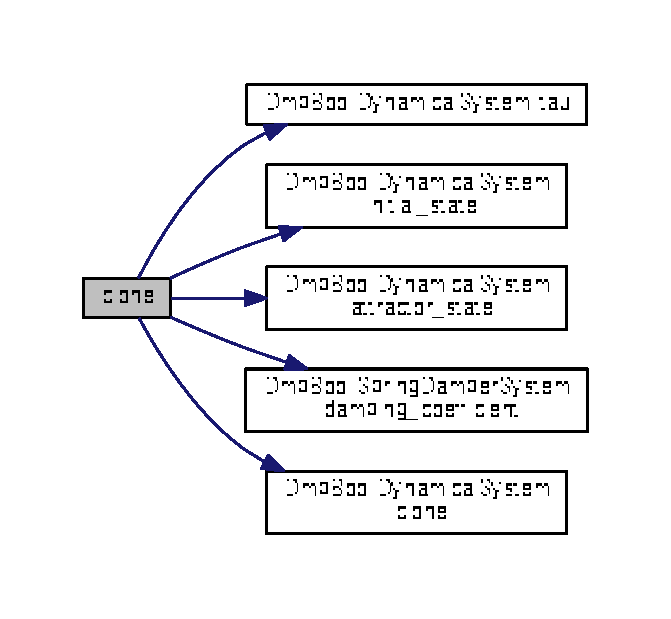
\includegraphics[width=322pt]{classDmpBbo_1_1Dmp_ace8e32350e4feb2c7ea6b5153c7dc606_cgraph}
\end{center}
\end{figure}


\hypertarget{classDmpBbo_1_1Dmp_a44dd496535fde494d8465e7603c93db3}{\index{Dmp\+Bbo\+::\+Dmp@{Dmp\+Bbo\+::\+Dmp}!integrate\+Start@{integrate\+Start}}
\index{integrate\+Start@{integrate\+Start}!Dmp\+Bbo\+::\+Dmp@{Dmp\+Bbo\+::\+Dmp}}
\paragraph[{integrate\+Start}]{\setlength{\rightskip}{0pt plus 5cm}void integrate\+Start (
\begin{DoxyParamCaption}
\item[{Eigen\+::\+Ref$<$ Eigen\+::\+Vector\+Xd $>$}]{x, }
\item[{Eigen\+::\+Ref$<$ Eigen\+::\+Vector\+Xd $>$}]{xd}
\end{DoxyParamCaption}
) const\hspace{0.3cm}{\ttfamily [virtual]}}}\label{classDmpBbo_1_1Dmp_a44dd496535fde494d8465e7603c93db3}


Start integrating the system. 


\begin{DoxyParams}[1]{Parameters}
\mbox{\tt out}  & {\em x} & -\/ The first vector of state variables \\
\hline
\mbox{\tt out}  & {\em xd} & -\/ The first vector of rates of change of the state variables\\
\hline
\end{DoxyParams}
\begin{DoxyRemark}{Remarks}
x and xd should be of size \hyperlink{group__DynamicalSystems_ga6f628f7f4ed9d77bf69f5b8560b98f18}{dim()} X 1. This forces you to pre-\/allocate memory, which speeds things up (and also makes Eigen's Ref functionality easier to deal with). 
\end{DoxyRemark}


Reimplemented from \hyperlink{classDmpBbo_1_1DynamicalSystem_a44dd496535fde494d8465e7603c93db3}{Dynamical\+System}.



Definition at line 248 of file Dmp.\+cpp.


\begin{DoxyCode}
249 \{
250   assert(x.size()==\hyperlink{group__DynamicalSystems_ga6f628f7f4ed9d77bf69f5b8560b98f18}{dim}());
251   assert(xd.size()==\hyperlink{group__DynamicalSystems_ga6f628f7f4ed9d77bf69f5b8560b98f18}{dim}());
252   
253   x.fill(0);  
254   xd.fill(0);  
255   
256   \textcolor{comment}{// Start integrating goal system if it exists}
257   \textcolor{keywordflow}{if} (goal\_system\_==NULL)
258   \{
259     \textcolor{comment}{// No goal system, simply set goal state to attractor state}
260     x.GOAL = \hyperlink{group__DynamicalSystems_gaebe3c462bc4a725cb17bcc3d13285f13}{attractor\_state}();
261     xd.GOAL.fill(0);
262   \}
263   \textcolor{keywordflow}{else}
264   \{
265     \textcolor{comment}{// Goal system exists. Start integrating it.}
266     goal\_system\_->\hyperlink{classDmpBbo_1_1DynamicalSystem_a44dd496535fde494d8465e7603c93db3}{integrateStart}(x.GOAL,xd.GOAL);
267   \}
268   
269     
270   \textcolor{comment}{// Set the attractor state of the spring system}
271   spring\_system\_->\hyperlink{group__DynamicalSystems_ga32a975e60b5f001308368c7f06b90e18}{set\_attractor\_state}(x.GOAL);
272   
273   \textcolor{comment}{// Start integrating all futher subsystems}
274   spring\_system\_->\hyperlink{classDmpBbo_1_1DynamicalSystem_a44dd496535fde494d8465e7603c93db3}{integrateStart}(x.SPRING, xd.SPRING);
275   phase\_system\_->\hyperlink{classDmpBbo_1_1DynamicalSystem_a44dd496535fde494d8465e7603c93db3}{integrateStart}(  x.PHASE,  xd.PHASE);
276   gating\_system\_->\hyperlink{classDmpBbo_1_1DynamicalSystem_a44dd496535fde494d8465e7603c93db3}{integrateStart}(x.GATING, xd.GATING);
277 
278   \textcolor{comment}{// Add rates of change}
279   \hyperlink{classDmpBbo_1_1Dmp_ab564468764e7e4dc7c11e2a786e22c19}{differentialEquation}(x,xd);
280   
281 \}
\end{DoxyCode}


Here is the call graph for this function\+:
\nopagebreak
\begin{figure}[H]
\begin{center}
\leavevmode
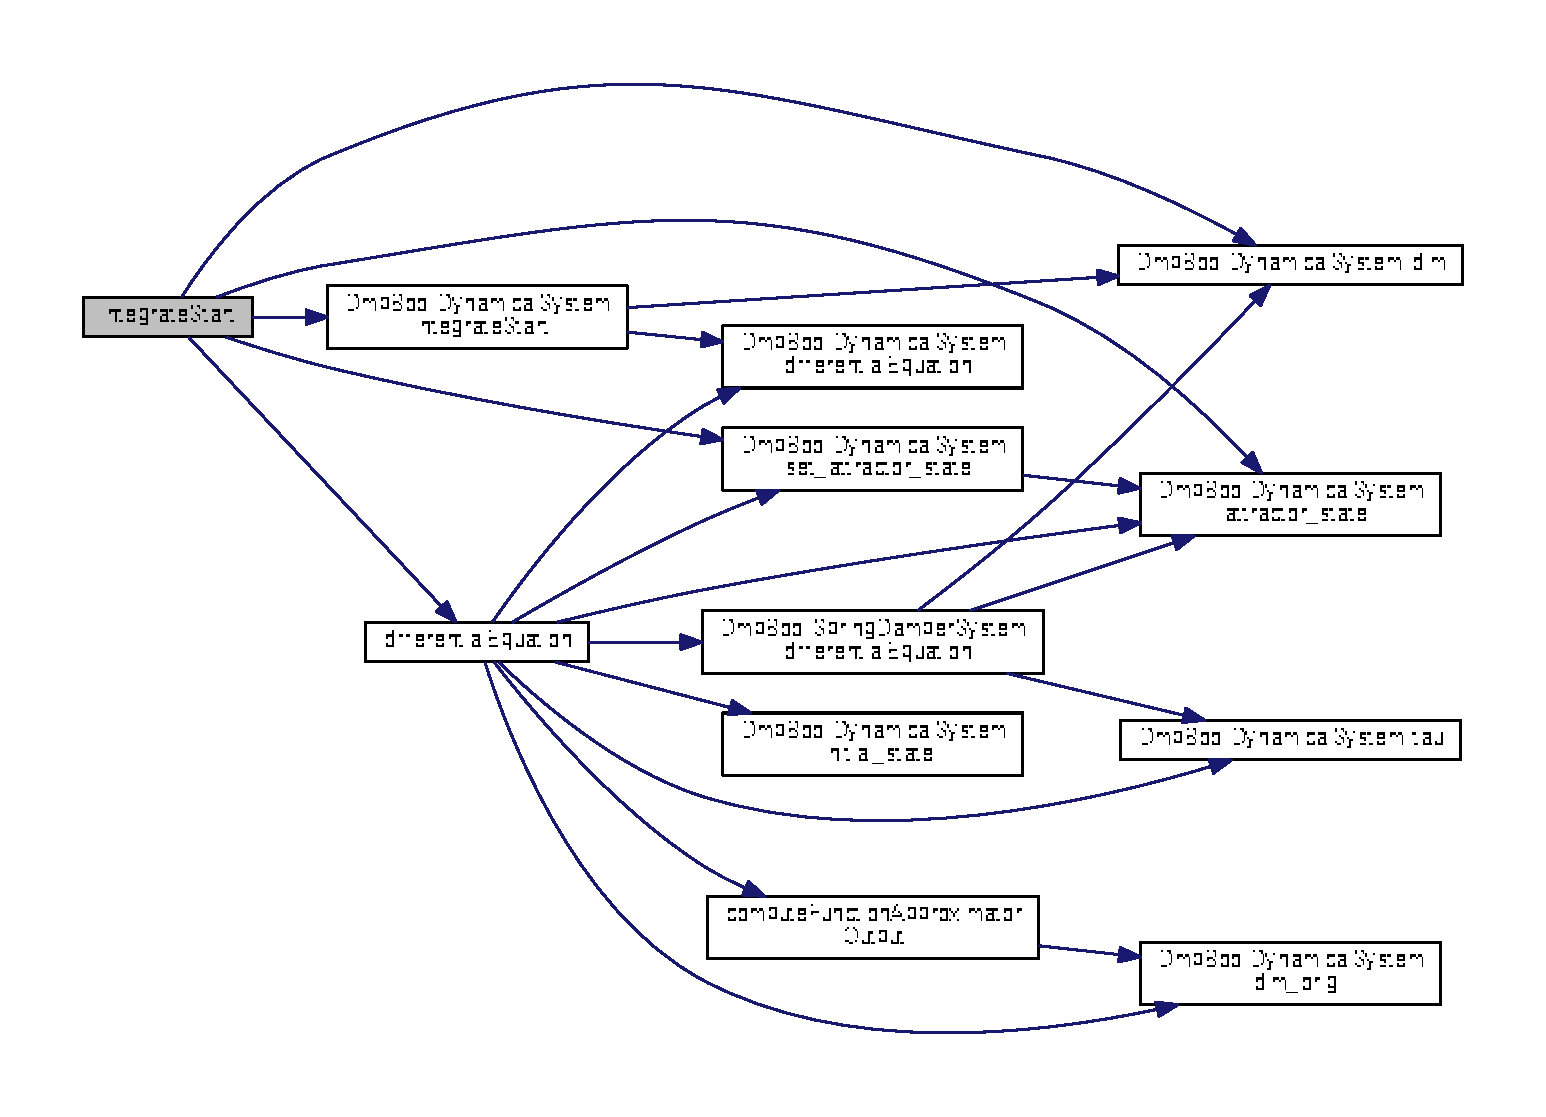
\includegraphics[width=350pt]{classDmpBbo_1_1Dmp_a44dd496535fde494d8465e7603c93db3_cgraph}
\end{center}
\end{figure}


\hypertarget{classDmpBbo_1_1Dmp_ab564468764e7e4dc7c11e2a786e22c19}{\index{Dmp\+Bbo\+::\+Dmp@{Dmp\+Bbo\+::\+Dmp}!differential\+Equation@{differential\+Equation}}
\index{differential\+Equation@{differential\+Equation}!Dmp\+Bbo\+::\+Dmp@{Dmp\+Bbo\+::\+Dmp}}
\paragraph[{differential\+Equation}]{\setlength{\rightskip}{0pt plus 5cm}void differential\+Equation (
\begin{DoxyParamCaption}
\item[{const Eigen\+::\+Vector\+Xd \&}]{x, }
\item[{Eigen\+::\+Ref$<$ Eigen\+::\+Vector\+Xd $>$}]{xd}
\end{DoxyParamCaption}
) const\hspace{0.3cm}{\ttfamily [virtual]}}}\label{classDmpBbo_1_1Dmp_ab564468764e7e4dc7c11e2a786e22c19}


The differential equation which defines the system. 

It relates state values to rates of change of those state values


\begin{DoxyParams}[1]{Parameters}
\mbox{\tt in}  & {\em x} & current state (column vector of size \hyperlink{group__DynamicalSystems_ga6f628f7f4ed9d77bf69f5b8560b98f18}{dim()} X 1) \\
\hline
\mbox{\tt out}  & {\em xd} & rate of change in state (column vector of size \hyperlink{group__DynamicalSystems_ga6f628f7f4ed9d77bf69f5b8560b98f18}{dim()} X 1)\\
\hline
\end{DoxyParams}
\begin{DoxyRemark}{Remarks}
x and xd should be of size \hyperlink{group__DynamicalSystems_ga6f628f7f4ed9d77bf69f5b8560b98f18}{dim()} X 1. This forces you to pre-\/allocate memory, which speeds things up (and also makes Eigen's Ref functionality easier to deal with). 
\end{DoxyRemark}


Implements \hyperlink{classDmpBbo_1_1DynamicalSystem_a70acc98a8e024f9b6e0e6de1b519e260}{Dynamical\+System}.



Definition at line 318 of file Dmp.\+cpp.


\begin{DoxyCode}
319 \{
320   
321   \textcolor{keywordflow}{if} (goal\_system\_==NULL)
322   \{
323     \textcolor{comment}{// If there is no dynamical system for the delayed goal, the goal is}
324     \textcolor{comment}{// simply the attractor state}
325     spring\_system\_->\hyperlink{group__DynamicalSystems_ga32a975e60b5f001308368c7f06b90e18}{set\_attractor\_state}(\hyperlink{group__DynamicalSystems_gaebe3c462bc4a725cb17bcc3d13285f13}{attractor\_state}());
326     \textcolor{comment}{// with zero change}
327     xd.GOAL.fill(0);
328   \} 
329   \textcolor{keywordflow}{else}
330   \{
331     \textcolor{comment}{// Integrate goal system and get current goal state}
332     goal\_system\_->\hyperlink{group__DynamicalSystems_ga32a975e60b5f001308368c7f06b90e18}{set\_attractor\_state}(\hyperlink{group__DynamicalSystems_gaebe3c462bc4a725cb17bcc3d13285f13}{attractor\_state}());
333     goal\_system\_->\hyperlink{classDmpBbo_1_1DynamicalSystem_a70acc98a8e024f9b6e0e6de1b519e260}{differentialEquation}(x.GOAL, xd.GOAL);
334     \textcolor{comment}{// The goal state is the attractor state of the spring-damper system}
335     spring\_system\_->\hyperlink{group__DynamicalSystems_ga32a975e60b5f001308368c7f06b90e18}{set\_attractor\_state}(x.GOAL);
336         
337   \}
338 
339   \textcolor{comment}{// Integrate spring damper system}
340   \textcolor{comment}{// Forcing term is added to spring\_state later}
341   spring\_system\_->\hyperlink{classDmpBbo_1_1SpringDamperSystem_ab564468764e7e4dc7c11e2a786e22c19}{differentialEquation}(x.SPRING, xd.SPRING);
342 
343   
344   \textcolor{comment}{// Non-linear forcing term}
345   phase\_system\_->\hyperlink{classDmpBbo_1_1DynamicalSystem_a70acc98a8e024f9b6e0e6de1b519e260}{differentialEquation}(x.PHASE, xd.PHASE);
346   gating\_system\_->\hyperlink{classDmpBbo_1_1DynamicalSystem_a70acc98a8e024f9b6e0e6de1b519e260}{differentialEquation}(x.GATING, xd.GATING);
347 
348   MatrixXd phase\_state(1,1);
349   phase\_state = x.PHASE;
350   MatrixXd fa\_output(1,\hyperlink{group__DynamicalSystems_ga93d7cbbf2e471b00f124e41706405a05}{dim\_orig}());
351   \hyperlink{classDmpBbo_1_1Dmp_a89078b732a4579130e24e3bc59c1713c}{computeFunctionApproximatorOutput}(phase\_state, fa\_output); 
352   
353   \textcolor{keywordtype}{int} t0 = 0;
354   \textcolor{keywordtype}{double} gating = (x.GATING)[0];
355   VectorXd g\_minus\_y0 = (\hyperlink{group__DynamicalSystems_gaebe3c462bc4a725cb17bcc3d13285f13}{attractor\_state}()-\hyperlink{group__DynamicalSystems_ga4c7f24e7deec1629548a075015bdc693}{initial\_state}()).transpose();
356   VectorXd forcing\_term = gating*fa\_output.row(t0); \textcolor{comment}{// todo .array()*g\_minus\_y0.array();}
357 
358   \textcolor{comment}{// Add forcing term to the ZD component of the spring state}
359   xd.SPRING\_Z = xd.SPRING\_Z + forcing\_term/\hyperlink{group__DynamicalSystems_ga50eec7ad4c9664b5809ace45b22200d5}{tau}();
360 
361 
362 \}
\end{DoxyCode}


Here is the call graph for this function\+:
\nopagebreak
\begin{figure}[H]
\begin{center}
\leavevmode
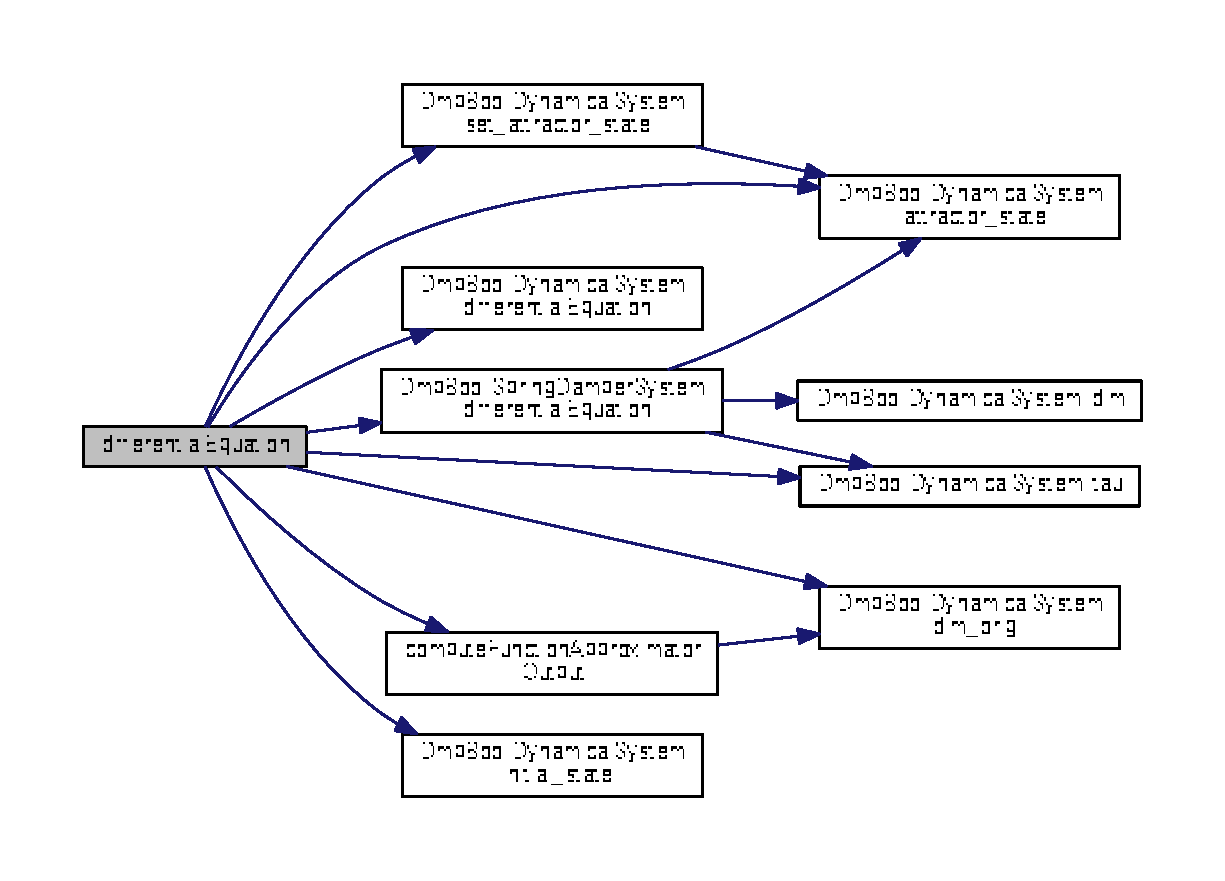
\includegraphics[width=350pt]{classDmpBbo_1_1Dmp_ab564468764e7e4dc7c11e2a786e22c19_cgraph}
\end{center}
\end{figure}


\hypertarget{classDmpBbo_1_1Dmp_ad62585b1e0bab2b9743782e15e01d694}{\index{Dmp\+Bbo\+::\+Dmp@{Dmp\+Bbo\+::\+Dmp}!analytical\+Solution@{analytical\+Solution}}
\index{analytical\+Solution@{analytical\+Solution}!Dmp\+Bbo\+::\+Dmp@{Dmp\+Bbo\+::\+Dmp}}
\paragraph[{analytical\+Solution}]{\setlength{\rightskip}{0pt plus 5cm}void analytical\+Solution (
\begin{DoxyParamCaption}
\item[{const Eigen\+::\+Vector\+Xd \&}]{ts, }
\item[{Eigen\+::\+Matrix\+Xd \&}]{xs, }
\item[{Eigen\+::\+Matrix\+Xd \&}]{xds, }
\item[{Eigen\+::\+Matrix\+Xd \&}]{forcing\+\_\+terms, }
\item[{Eigen\+::\+Matrix\+Xd \&}]{fa\+\_\+output}
\end{DoxyParamCaption}
) const}}\label{classDmpBbo_1_1Dmp_ad62585b1e0bab2b9743782e15e01d694}


Return analytical solution of the system at certain times (and return forcing terms) 


\begin{DoxyParams}[1]{Parameters}
\mbox{\tt in}  & {\em ts} & A vector of times for which to compute the analytical solutions \\
\hline
\mbox{\tt out}  & {\em xs} & Sequence of state vectors. T x D or D x T matrix, where T is the number of times (the length of 'ts'), and D the size of the state (i.\+e. \hyperlink{group__DynamicalSystems_ga6f628f7f4ed9d77bf69f5b8560b98f18}{dim()}) \\
\hline
\mbox{\tt out}  & {\em xds} & Sequence of state vectors (rates of change). T x D or D x T matrix, where T is the number of times (the length of 'ts'), and D the size of the state (i.\+e. \hyperlink{group__DynamicalSystems_ga6f628f7f4ed9d77bf69f5b8560b98f18}{dim()}) \\
\hline
\mbox{\tt out}  & {\em forcing\+\_\+terms} & The forcing terms for each dimension, for debugging purposes only. \\
\hline
\mbox{\tt out}  & {\em fa\+\_\+output} & The output of the function approximators, for debugging purposes only.\\
\hline
\end{DoxyParams}
\begin{DoxyRemark}{Remarks}
The output xs and xds will be of size D x T {\itshape only} if the matrix x you pass as an argument of size D x T. In all other cases (i.\+e. including passing an empty matrix) the size of x will be T x D. This feature has been added so that you may pass matrices of either size. 
\end{DoxyRemark}


Definition at line 403 of file Dmp.\+cpp.


\begin{DoxyCode}
404 \{
405   \textcolor{keywordtype}{int} n\_time\_steps = ts.size();
406   assert(n\_time\_steps>0);
407   
408   \textcolor{comment}{// Usually, we expect xs and xds to be of size T X dim(), so we resize to that. However, if the}
409   \textcolor{comment}{// input matrices were of size dim() X T, we return the matrices of that size by doing a }
410   \textcolor{comment}{// transposeInPlace at the end. That way, the user can also request dim() X T sized matrices.}
411   \textcolor{keywordtype}{bool} caller\_expects\_transposed = (xs.rows()==\hyperlink{group__DynamicalSystems_ga6f628f7f4ed9d77bf69f5b8560b98f18}{dim}() && xs.cols()==n\_time\_steps);
412   
413   \textcolor{comment}{// INTEGRATE SYSTEMS ANALYTICALLY AS MUCH AS POSSIBLE}
414 
415   \textcolor{comment}{// Integrate phase}
416   MatrixXd xs\_phase;
417   MatrixXd xds\_phase;
418   phase\_system\_->\hyperlink{classDmpBbo_1_1DynamicalSystem_ab6092038efc51ebd122e7c0878f6557d}{analyticalSolution}(ts,xs\_phase,xds\_phase);
419   
420   \textcolor{comment}{// Compute gating term}
421   MatrixXd xs\_gating;
422   MatrixXd xds\_gating;
423   gating\_system\_->\hyperlink{classDmpBbo_1_1DynamicalSystem_ab6092038efc51ebd122e7c0878f6557d}{analyticalSolution}(ts,xs\_gating,xds\_gating);
424 
425   \textcolor{comment}{// Compute the output of the function approximator}
426   fa\_outputs.resize(ts.size(),\hyperlink{group__DynamicalSystems_ga93d7cbbf2e471b00f124e41706405a05}{dim\_orig}());
427   fa\_outputs.fill(0.0);
428   \textcolor{comment}{//if (isTrained())}
429   \hyperlink{classDmpBbo_1_1Dmp_a89078b732a4579130e24e3bc59c1713c}{computeFunctionApproximatorOutput}(xs\_phase, fa\_outputs);
430 
431   MatrixXd xs\_gating\_rep = xs\_gating.replicate(1,fa\_outputs.cols());
432   MatrixXd g\_minus\_y0\_rep = (\hyperlink{group__DynamicalSystems_gaebe3c462bc4a725cb17bcc3d13285f13}{attractor\_state}()-\hyperlink{group__DynamicalSystems_ga4c7f24e7deec1629548a075015bdc693}{initial\_state}()).transpose().
      replicate(n\_time\_steps,1);
433   forcing\_terms = fa\_outputs.array()*xs\_gating\_rep.array(); \textcolor{comment}{// todo *g\_minus\_y0\_rep.array();}
434   
435   MatrixXd xs\_goal, xds\_goal;
436   \textcolor{comment}{// Get current delayed goal}
437   \textcolor{keywordflow}{if} (goal\_system\_==NULL)
438   \{
439     \textcolor{comment}{// If there is no dynamical system for the delayed goal, the goal is}
440     \textcolor{comment}{// simply the attractor state               }
441     xs\_goal  = \hyperlink{group__DynamicalSystems_gaebe3c462bc4a725cb17bcc3d13285f13}{attractor\_state}().transpose().replicate(n\_time\_steps,1);
442     \textcolor{comment}{// with zero change}
443     xds\_goal = MatrixXd::Zero(n\_time\_steps,\hyperlink{group__DynamicalSystems_ga93d7cbbf2e471b00f124e41706405a05}{dim\_orig}());
444   \} 
445   \textcolor{keywordflow}{else}
446   \{
447     \textcolor{comment}{// Integrate goal system and get current goal state}
448     goal\_system\_->\hyperlink{classDmpBbo_1_1DynamicalSystem_ab6092038efc51ebd122e7c0878f6557d}{analyticalSolution}(ts,xs\_goal,xds\_goal);
449   \}
450 
451   xs.resize(n\_time\_steps,\hyperlink{group__DynamicalSystems_ga6f628f7f4ed9d77bf69f5b8560b98f18}{dim}());
452   xds.resize(n\_time\_steps,\hyperlink{group__DynamicalSystems_ga6f628f7f4ed9d77bf69f5b8560b98f18}{dim}());
453 
454   \textcolor{keywordtype}{int} T = n\_time\_steps;
455     
456   xs.GOALM(T) = xs\_goal;     xds.GOALM(T) = xds\_goal;
457   xs.PHASEM(T) = xs\_phase;   xds.PHASEM(T) = xds\_phase;
458   xs.GATINGM(T) = xs\_gating; xds.GATINGM(T) = xds\_gating;
459 
460   
461   \textcolor{comment}{// THE REST CANNOT BE DONE ANALYTICALLY}
462   
463   \textcolor{comment}{// Reset the dynamical system, and get the first state}
464   \textcolor{keywordtype}{double} damping = spring\_system\_->\hyperlink{classDmpBbo_1_1SpringDamperSystem_a1e0acb1d6298104e74f81f53768f5bf1}{damping\_coefficient}();
465   SpringDamperSystem localspring\_system\_(\hyperlink{group__DynamicalSystems_ga50eec7ad4c9664b5809ace45b22200d5}{tau}(),\hyperlink{group__DynamicalSystems_ga4c7f24e7deec1629548a075015bdc693}{initial\_state}(),
      \hyperlink{group__DynamicalSystems_gaebe3c462bc4a725cb17bcc3d13285f13}{attractor\_state}(),damping);
466   
467   \textcolor{comment}{// Set first attractor state}
468   localspring\_system\_.set\_attractor\_state(xs\_goal.row(0));
469   
470   \textcolor{comment}{// Start integrating spring damper system}
471   \textcolor{keywordtype}{int} dim\_spring = localspring\_system\_.dim();
472   VectorXd x\_spring(dim\_spring), xd\_spring(dim\_spring); \textcolor{comment}{// todo Why are these needed?}
473   \textcolor{keywordtype}{int} t0 = 0;
474   localspring\_system\_.integrateStart(x\_spring, xd\_spring);
475   xs.row(t0).SPRING  = x\_spring;
476   xds.row(t0).SPRING = xd\_spring;
477 
478   \textcolor{comment}{// Add forcing term to the acceleration of the spring state  }
479   xds.SPRINGM\_Z(1) = xds.SPRINGM\_Z(1) + forcing\_terms.row(t0)/\hyperlink{group__DynamicalSystems_ga50eec7ad4c9664b5809ace45b22200d5}{tau}();
480   
481   \textcolor{keywordflow}{for} (\textcolor{keywordtype}{int} tt=1; tt<n\_time\_steps; tt++)
482   \{
483     \textcolor{keywordtype}{double} dt = ts[tt]-ts[tt-1];
484     
485     \textcolor{comment}{// Euler integration}
486     xs.row(tt).SPRING  = xs.row(tt-1).SPRING + dt*xds.row(tt-1).SPRING;
487   
488     \textcolor{comment}{// Set the attractor state of the spring system}
489     localspring\_system\_.set\_attractor\_state(xs.row(tt).GOAL);
490 
491     \textcolor{comment}{// Integrate spring damper system}
492     localspring\_system\_.differentialEquation(xs.row(tt).SPRING, xd\_spring);
493     xds.row(tt).SPRING = xd\_spring;
494     
495     \textcolor{comment}{// If necessary add a perturbation. May be useful for some off-line tests.}
496     RowVectorXd perturbation = RowVectorXd::Constant(\hyperlink{group__DynamicalSystems_ga93d7cbbf2e471b00f124e41706405a05}{dim\_orig}(),0.0);
497     \textcolor{keywordflow}{if} (analytical\_solution\_perturber\_!=NULL)
498       \textcolor{keywordflow}{for} (\textcolor{keywordtype}{int} i\_dim=0; i\_dim<\hyperlink{group__DynamicalSystems_ga93d7cbbf2e471b00f124e41706405a05}{dim\_orig}(); i\_dim++)
499         \textcolor{comment}{// Sample perturbation from a normal Gaussian distribution}
500         perturbation(i\_dim) = (*analytical\_solution\_perturber\_)();
501       
502     \textcolor{comment}{// Add forcing term to the acceleration of the spring state}
503     xds.row(tt).SPRING\_Z = xds.row(tt).SPRING\_Z + forcing\_terms.row(tt)/\hyperlink{group__DynamicalSystems_ga50eec7ad4c9664b5809ace45b22200d5}{tau}() + perturbation;
504     \textcolor{comment}{// Compute y component from z}
505     xds.row(tt).SPRING\_Y = xs.row(tt).SPRING\_Z/\hyperlink{group__DynamicalSystems_ga50eec7ad4c9664b5809ace45b22200d5}{tau}();
506     
507   \} 
508   
509   \textcolor{keywordflow}{if} (caller\_expects\_transposed)
510   \{
511     xs.transposeInPlace();
512     xds.transposeInPlace();
513   \}
514 \}
\end{DoxyCode}


Here is the call graph for this function\+:
\nopagebreak
\begin{figure}[H]
\begin{center}
\leavevmode
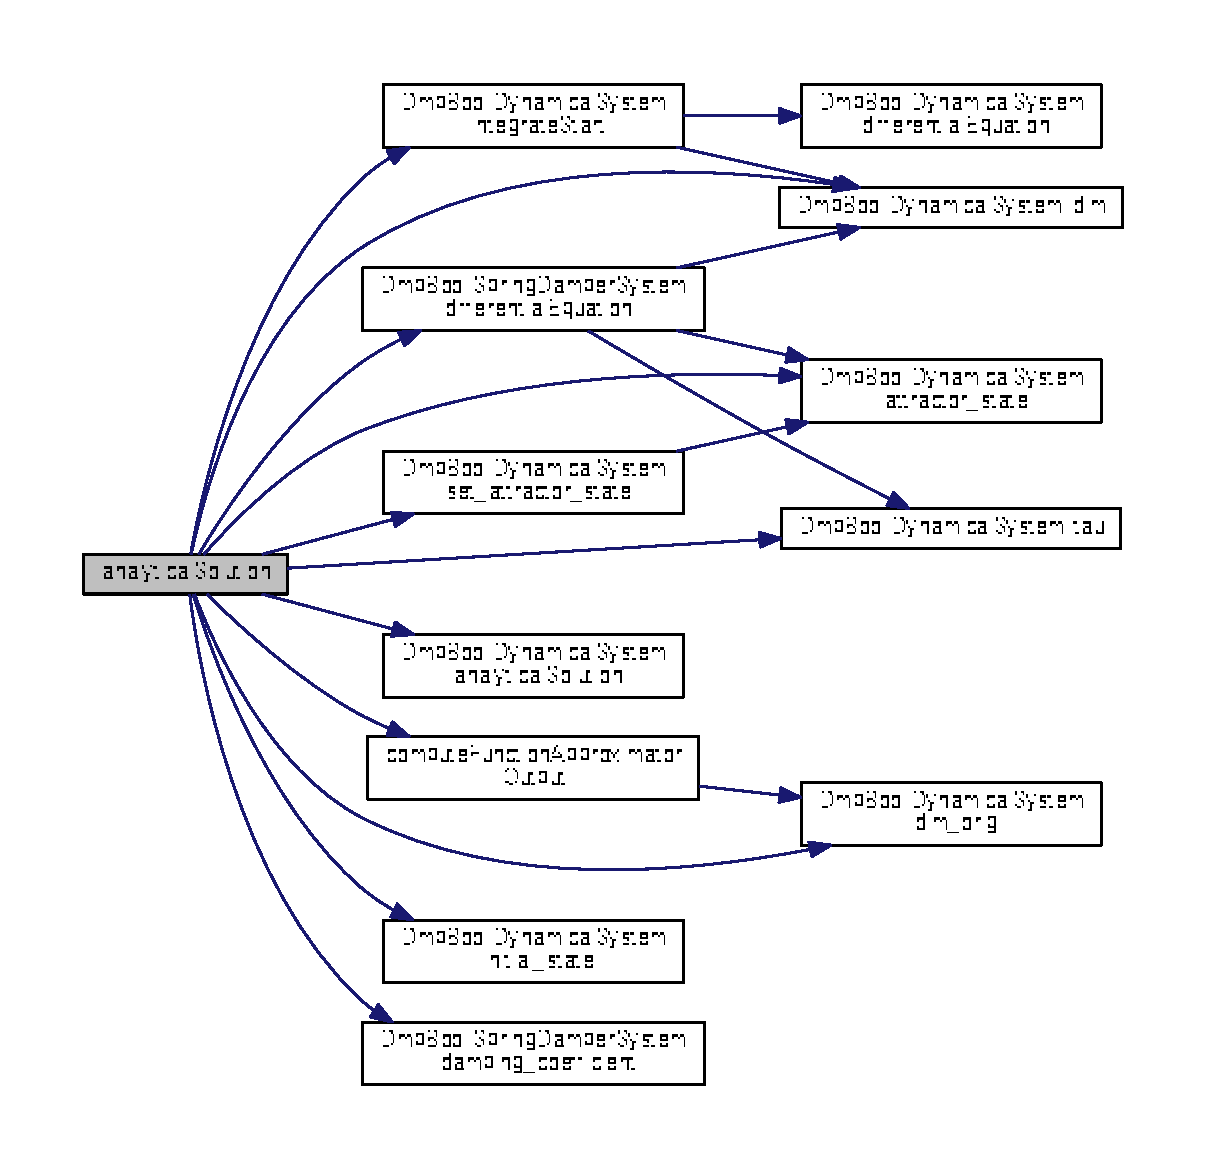
\includegraphics[width=350pt]{classDmpBbo_1_1Dmp_ad62585b1e0bab2b9743782e15e01d694_cgraph}
\end{center}
\end{figure}


\hypertarget{classDmpBbo_1_1Dmp_a636531b0dea01397d1338b19e0061360}{\index{Dmp\+Bbo\+::\+Dmp@{Dmp\+Bbo\+::\+Dmp}!analytical\+Solution@{analytical\+Solution}}
\index{analytical\+Solution@{analytical\+Solution}!Dmp\+Bbo\+::\+Dmp@{Dmp\+Bbo\+::\+Dmp}}
\paragraph[{analytical\+Solution}]{\setlength{\rightskip}{0pt plus 5cm}void analytical\+Solution (
\begin{DoxyParamCaption}
\item[{const Eigen\+::\+Vector\+Xd \&}]{ts, }
\item[{Eigen\+::\+Matrix\+Xd \&}]{xs, }
\item[{Eigen\+::\+Matrix\+Xd \&}]{xds, }
\item[{Eigen\+::\+Matrix\+Xd \&}]{forcing\+\_\+terms}
\end{DoxyParamCaption}
) const\hspace{0.3cm}{\ttfamily [inline]}}}\label{classDmpBbo_1_1Dmp_a636531b0dea01397d1338b19e0061360}


Return analytical solution of the system at certain times (and return forcing terms) 


\begin{DoxyParams}[1]{Parameters}
\mbox{\tt in}  & {\em ts} & A vector of times for which to compute the analytical solutions \\
\hline
\mbox{\tt out}  & {\em xs} & Sequence of state vectors. T x D or D x T matrix, where T is the number of times (the length of 'ts'), and D the size of the state (i.\+e. \hyperlink{group__DynamicalSystems_ga6f628f7f4ed9d77bf69f5b8560b98f18}{dim()}) \\
\hline
\mbox{\tt out}  & {\em xds} & Sequence of state vectors (rates of change). T x D or D x T matrix, where T is the number of times (the length of 'ts'), and D the size of the state (i.\+e. \hyperlink{group__DynamicalSystems_ga6f628f7f4ed9d77bf69f5b8560b98f18}{dim()}) \\
\hline
\mbox{\tt out}  & {\em forcing\+\_\+terms} & The forcing terms for each dimension, for debugging purposes only.\\
\hline
\end{DoxyParams}
\begin{DoxyRemark}{Remarks}
The output xs and xds will be of size D x T {\itshape only} if the matrix x you pass as an argument of size D x T. In all other cases (i.\+e. including passing an empty matrix) the size of x will be T x D. This feature has been added so that you may pass matrices of either size. 
\end{DoxyRemark}


Definition at line 157 of file Dmp.\+hpp.


\begin{DoxyCode}
158   \{
159     Eigen::MatrixXd fa\_output;
160     \hyperlink{classDmpBbo_1_1Dmp_ad62585b1e0bab2b9743782e15e01d694}{analyticalSolution}(ts, xs, xds, forcing\_terms, fa\_output);
161   \}
\end{DoxyCode}


Here is the call graph for this function\+:
\nopagebreak
\begin{figure}[H]
\begin{center}
\leavevmode
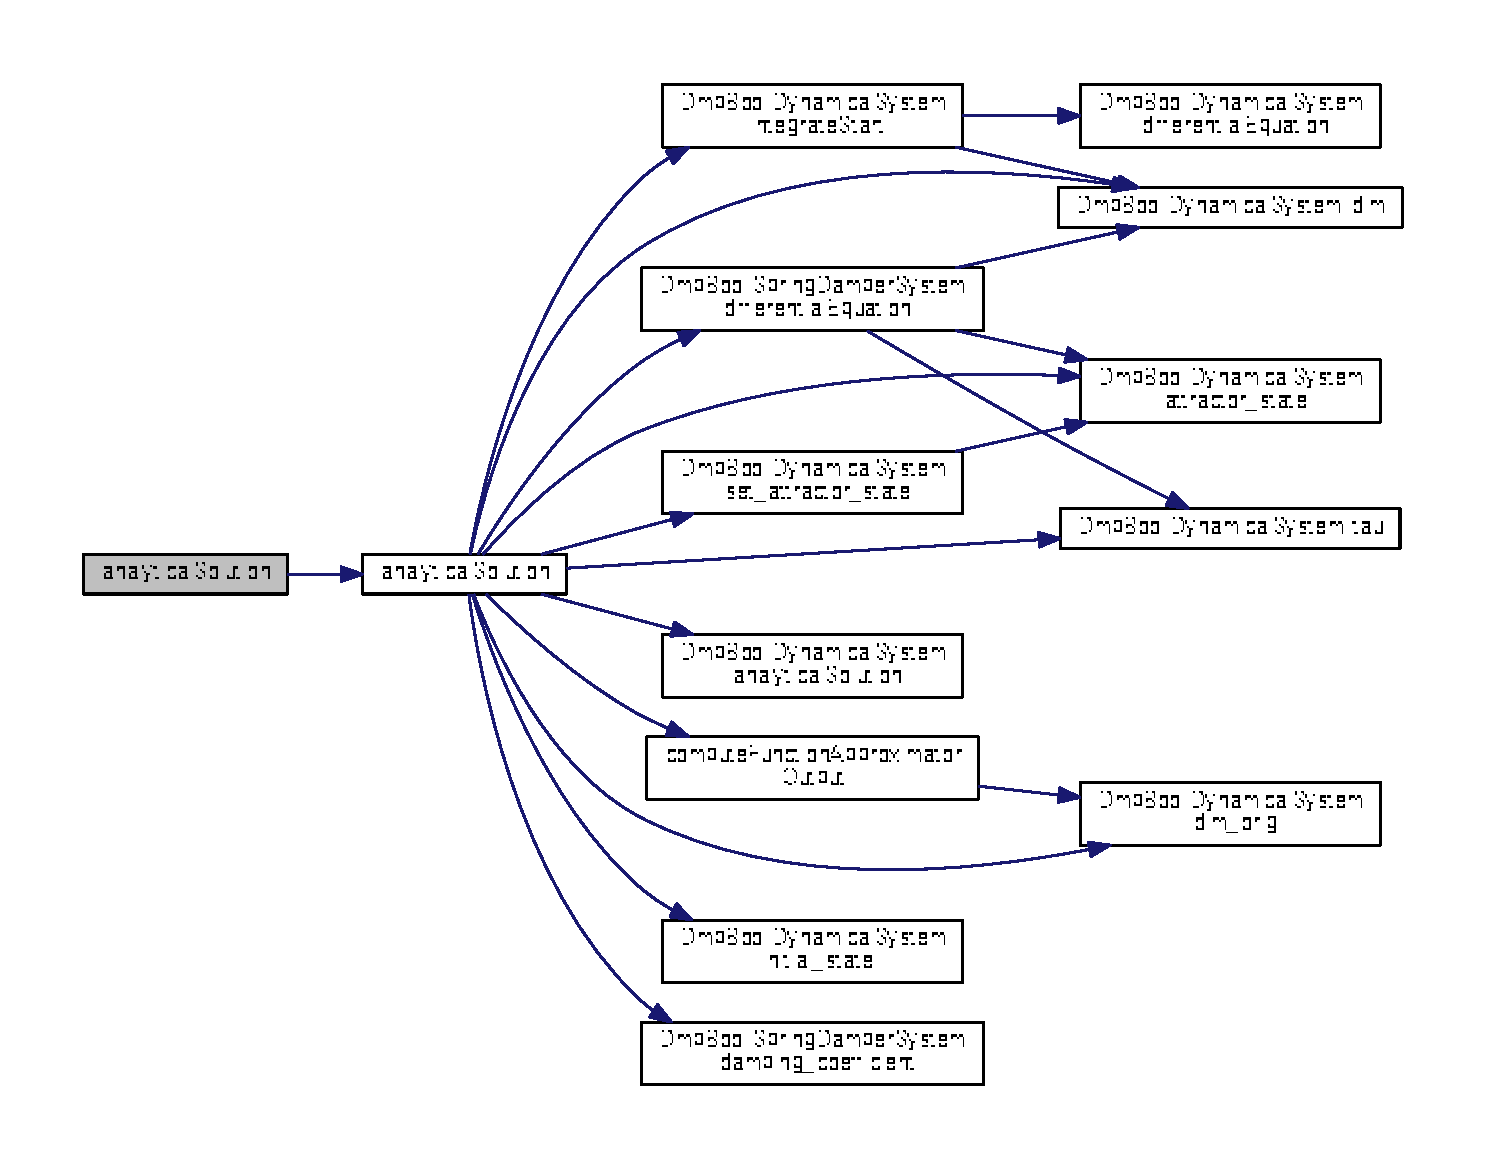
\includegraphics[width=350pt]{classDmpBbo_1_1Dmp_a636531b0dea01397d1338b19e0061360_cgraph}
\end{center}
\end{figure}


\hypertarget{classDmpBbo_1_1Dmp_ab6600b58b35bc9e66673d16f68e2e919}{\index{Dmp\+Bbo\+::\+Dmp@{Dmp\+Bbo\+::\+Dmp}!analytical\+Solution@{analytical\+Solution}}
\index{analytical\+Solution@{analytical\+Solution}!Dmp\+Bbo\+::\+Dmp@{Dmp\+Bbo\+::\+Dmp}}
\paragraph[{analytical\+Solution}]{\setlength{\rightskip}{0pt plus 5cm}void analytical\+Solution (
\begin{DoxyParamCaption}
\item[{const Eigen\+::\+Vector\+Xd \&}]{ts, }
\item[{Eigen\+::\+Matrix\+Xd \&}]{xs, }
\item[{Eigen\+::\+Matrix\+Xd \&}]{xds}
\end{DoxyParamCaption}
) const\hspace{0.3cm}{\ttfamily [inline]}, {\ttfamily [virtual]}}}\label{classDmpBbo_1_1Dmp_ab6600b58b35bc9e66673d16f68e2e919}


Return analytical solution of the system at certain times. 


\begin{DoxyParams}[1]{Parameters}
\mbox{\tt in}  & {\em ts} & A vector of times for which to compute the analytical solutions \\
\hline
\mbox{\tt out}  & {\em xs} & Sequence of state vectors. T x D or D x T matrix, where T is the number of times (the length of 'ts'), and D the size of the state (i.\+e. \hyperlink{group__DynamicalSystems_ga6f628f7f4ed9d77bf69f5b8560b98f18}{dim()}) \\
\hline
\mbox{\tt out}  & {\em xds} & Sequence of state vectors (rates of change). T x D or D x T matrix, where T is the number of times (the length of 'ts'), and D the size of the state (i.\+e. \hyperlink{group__DynamicalSystems_ga6f628f7f4ed9d77bf69f5b8560b98f18}{dim()})\\
\hline
\end{DoxyParams}
\begin{DoxyRemark}{Remarks}
The output xs and xds will be of size D x T {\itshape only} if the matrix x you pass as an argument of size D x T. In all other cases (i.\+e. including passing an empty matrix) the size of x will be T x D. This feature has been added so that you may pass matrices of either size. 
\end{DoxyRemark}


Implements \hyperlink{classDmpBbo_1_1DynamicalSystem_ab6092038efc51ebd122e7c0878f6557d}{Dynamical\+System}.



Definition at line 163 of file Dmp.\+hpp.


\begin{DoxyCode}
164   \{
165     Eigen::MatrixXd forcing\_terms, fa\_output;
166     \hyperlink{classDmpBbo_1_1Dmp_ad62585b1e0bab2b9743782e15e01d694}{analyticalSolution}(ts, xs, xds, forcing\_terms, fa\_output);
167   \}
\end{DoxyCode}


Here is the call graph for this function\+:
\nopagebreak
\begin{figure}[H]
\begin{center}
\leavevmode
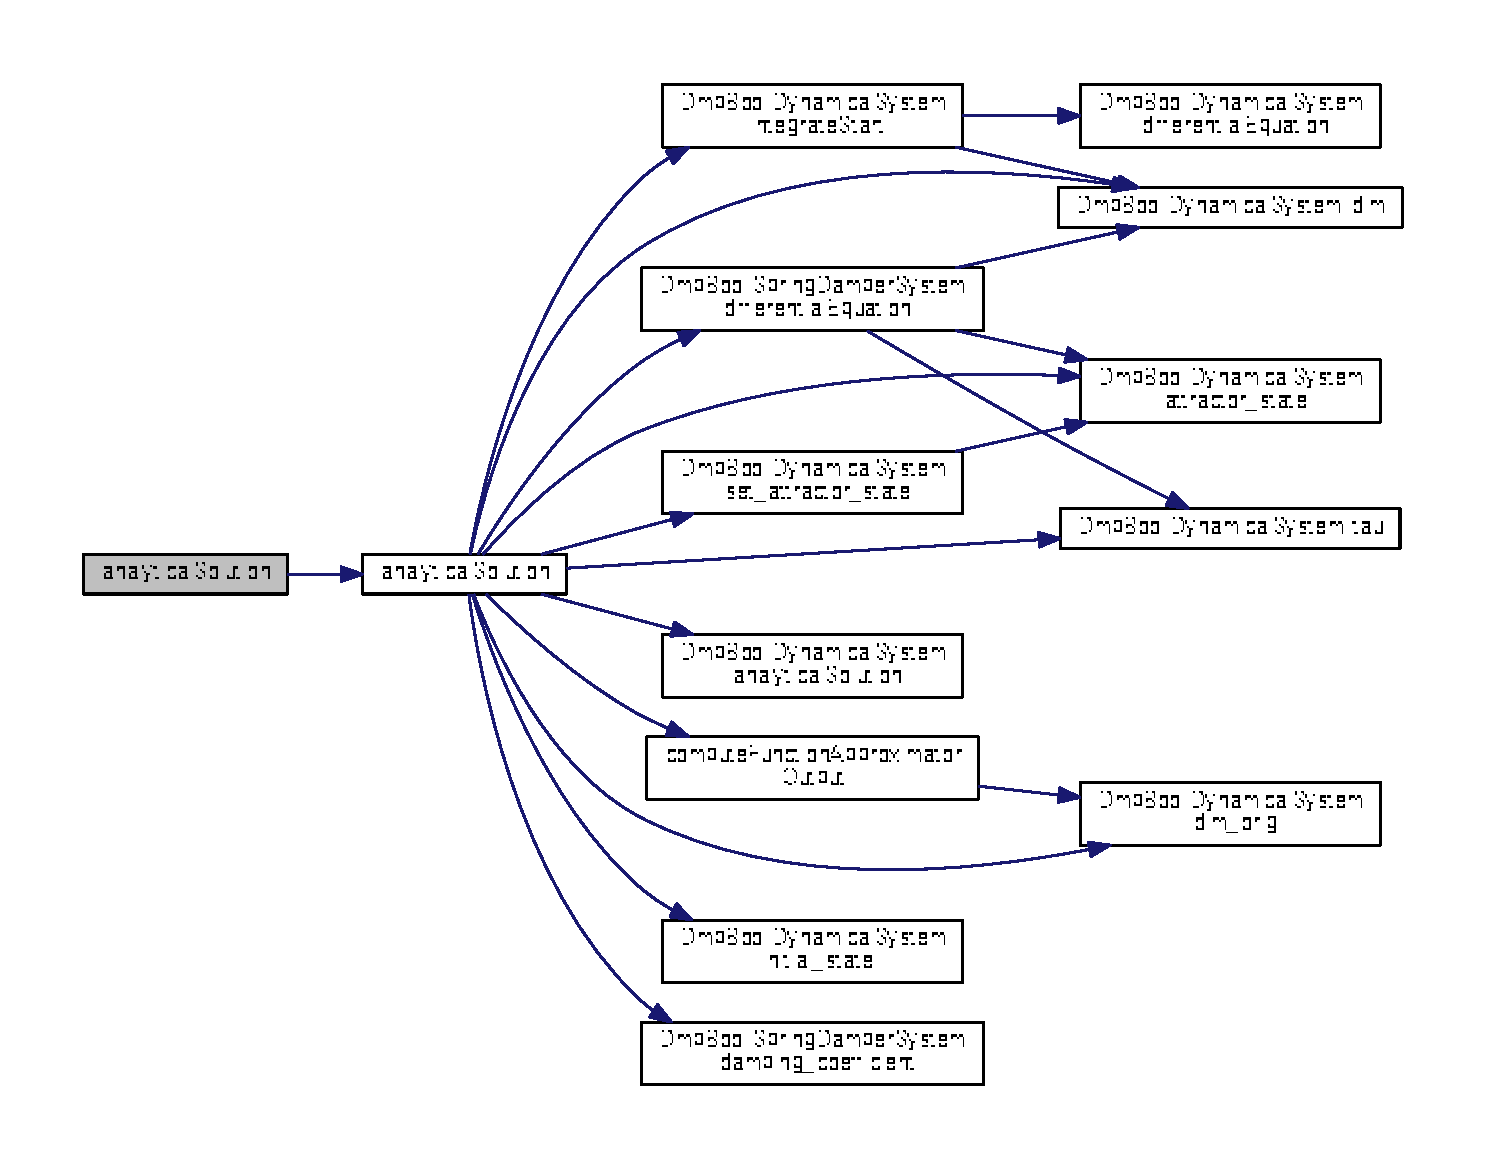
\includegraphics[width=350pt]{classDmpBbo_1_1Dmp_ab6600b58b35bc9e66673d16f68e2e919_cgraph}
\end{center}
\end{figure}


\hypertarget{classDmpBbo_1_1Dmp_a9b6bbda07ecd4fc7b6c9de57e185ab05}{\index{Dmp\+Bbo\+::\+Dmp@{Dmp\+Bbo\+::\+Dmp}!analytical\+Solution@{analytical\+Solution}}
\index{analytical\+Solution@{analytical\+Solution}!Dmp\+Bbo\+::\+Dmp@{Dmp\+Bbo\+::\+Dmp}}
\paragraph[{analytical\+Solution}]{\setlength{\rightskip}{0pt plus 5cm}void analytical\+Solution (
\begin{DoxyParamCaption}
\item[{const Eigen\+::\+Vector\+Xd \&}]{ts, }
\item[{{\bf Trajectory} \&}]{trajectory}
\end{DoxyParamCaption}
) const\hspace{0.3cm}{\ttfamily [inline]}}}\label{classDmpBbo_1_1Dmp_a9b6bbda07ecd4fc7b6c9de57e185ab05}


Return analytical solution of the system at certain times. 


\begin{DoxyParams}[1]{Parameters}
\mbox{\tt in}  & {\em ts} & A vector of times for which to compute the analytical solutions \\
\hline
\mbox{\tt out}  & {\em trajectory} & The computed states as a trajectory. \\
\hline
\end{DoxyParams}


Definition at line 175 of file Dmp.\+hpp.


\begin{DoxyCode}
176   \{
177     Eigen::MatrixXd xs,  xds;
178     \hyperlink{classDmpBbo_1_1Dmp_ad62585b1e0bab2b9743782e15e01d694}{analyticalSolution}(ts, xs, xds);
179     \hyperlink{classDmpBbo_1_1Dmp_aa3ad2fc66e8ce09cfa68032a4a5004b9}{statesAsTrajectory}(ts, xs, xds, trajectory);
180   \}
\end{DoxyCode}


Here is the call graph for this function\+:
\nopagebreak
\begin{figure}[H]
\begin{center}
\leavevmode
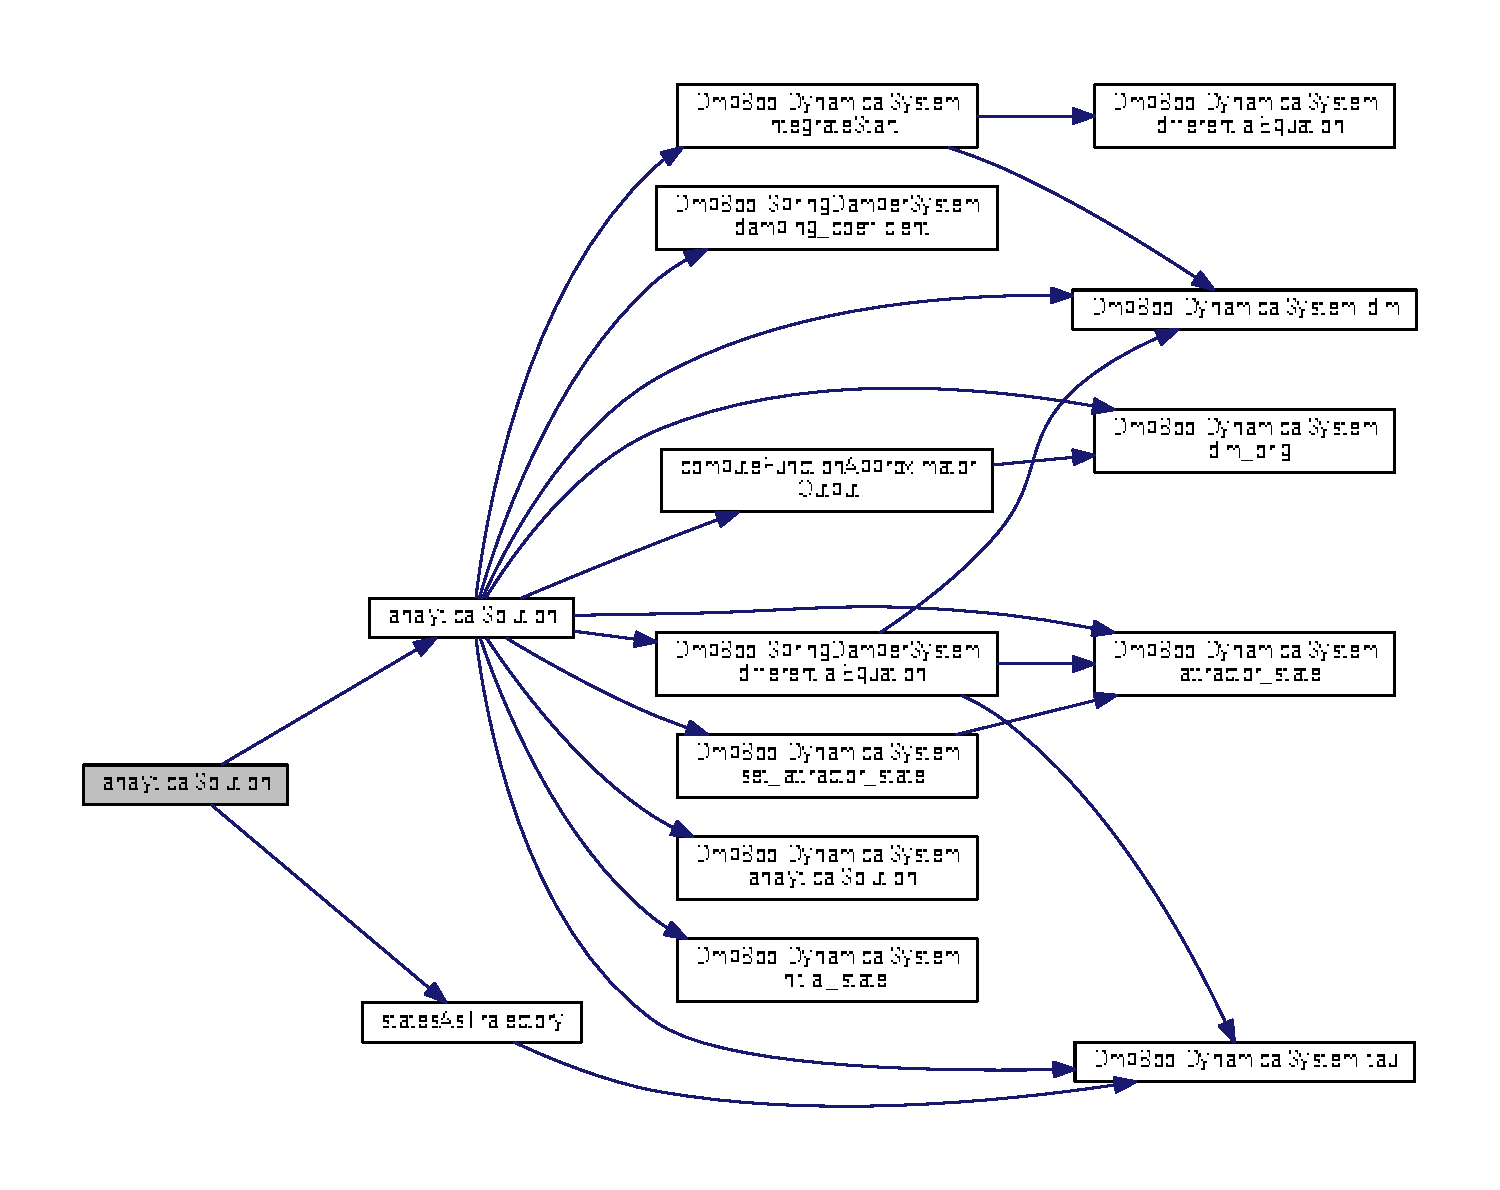
\includegraphics[width=350pt]{classDmpBbo_1_1Dmp_a9b6bbda07ecd4fc7b6c9de57e185ab05_cgraph}
\end{center}
\end{figure}


\hypertarget{classDmpBbo_1_1Dmp_ae1e5218e7ebfedf7fb2501dc8af2675f}{\index{Dmp\+Bbo\+::\+Dmp@{Dmp\+Bbo\+::\+Dmp}!analytical\+Solution@{analytical\+Solution}}
\index{analytical\+Solution@{analytical\+Solution}!Dmp\+Bbo\+::\+Dmp@{Dmp\+Bbo\+::\+Dmp}}
\paragraph[{analytical\+Solution}]{\setlength{\rightskip}{0pt plus 5cm}void analytical\+Solution (
\begin{DoxyParamCaption}
\item[{const Eigen\+::\+Vector\+Xd \&}]{ts, }
\item[{{\bf Trajectory} \&}]{trajectory, }
\item[{Eigen\+::\+Matrix\+Xd \&}]{forcing\+\_\+terms}
\end{DoxyParamCaption}
) const\hspace{0.3cm}{\ttfamily [inline]}}}\label{classDmpBbo_1_1Dmp_ae1e5218e7ebfedf7fb2501dc8af2675f}


Return analytical solution of the system at certain times. 


\begin{DoxyParams}[1]{Parameters}
\mbox{\tt in}  & {\em ts} & A vector of times for which to compute the analytical solutions \\
\hline
\mbox{\tt out}  & {\em trajectory} & The computed states as a trajectory. \\
\hline
\mbox{\tt out}  & {\em forcing\+\_\+terms} & The forcing terms \\
\hline
\end{DoxyParams}


Definition at line 189 of file Dmp.\+hpp.


\begin{DoxyCode}
190   \{
191     Eigen::MatrixXd xs,  xds;
192     \hyperlink{classDmpBbo_1_1Dmp_ad62585b1e0bab2b9743782e15e01d694}{analyticalSolution}(ts, xs, xds, forcing\_terms);
193     \hyperlink{classDmpBbo_1_1Dmp_aa3ad2fc66e8ce09cfa68032a4a5004b9}{statesAsTrajectory}(ts, xs, xds, trajectory);
194   \}
\end{DoxyCode}


Here is the call graph for this function\+:
\nopagebreak
\begin{figure}[H]
\begin{center}
\leavevmode
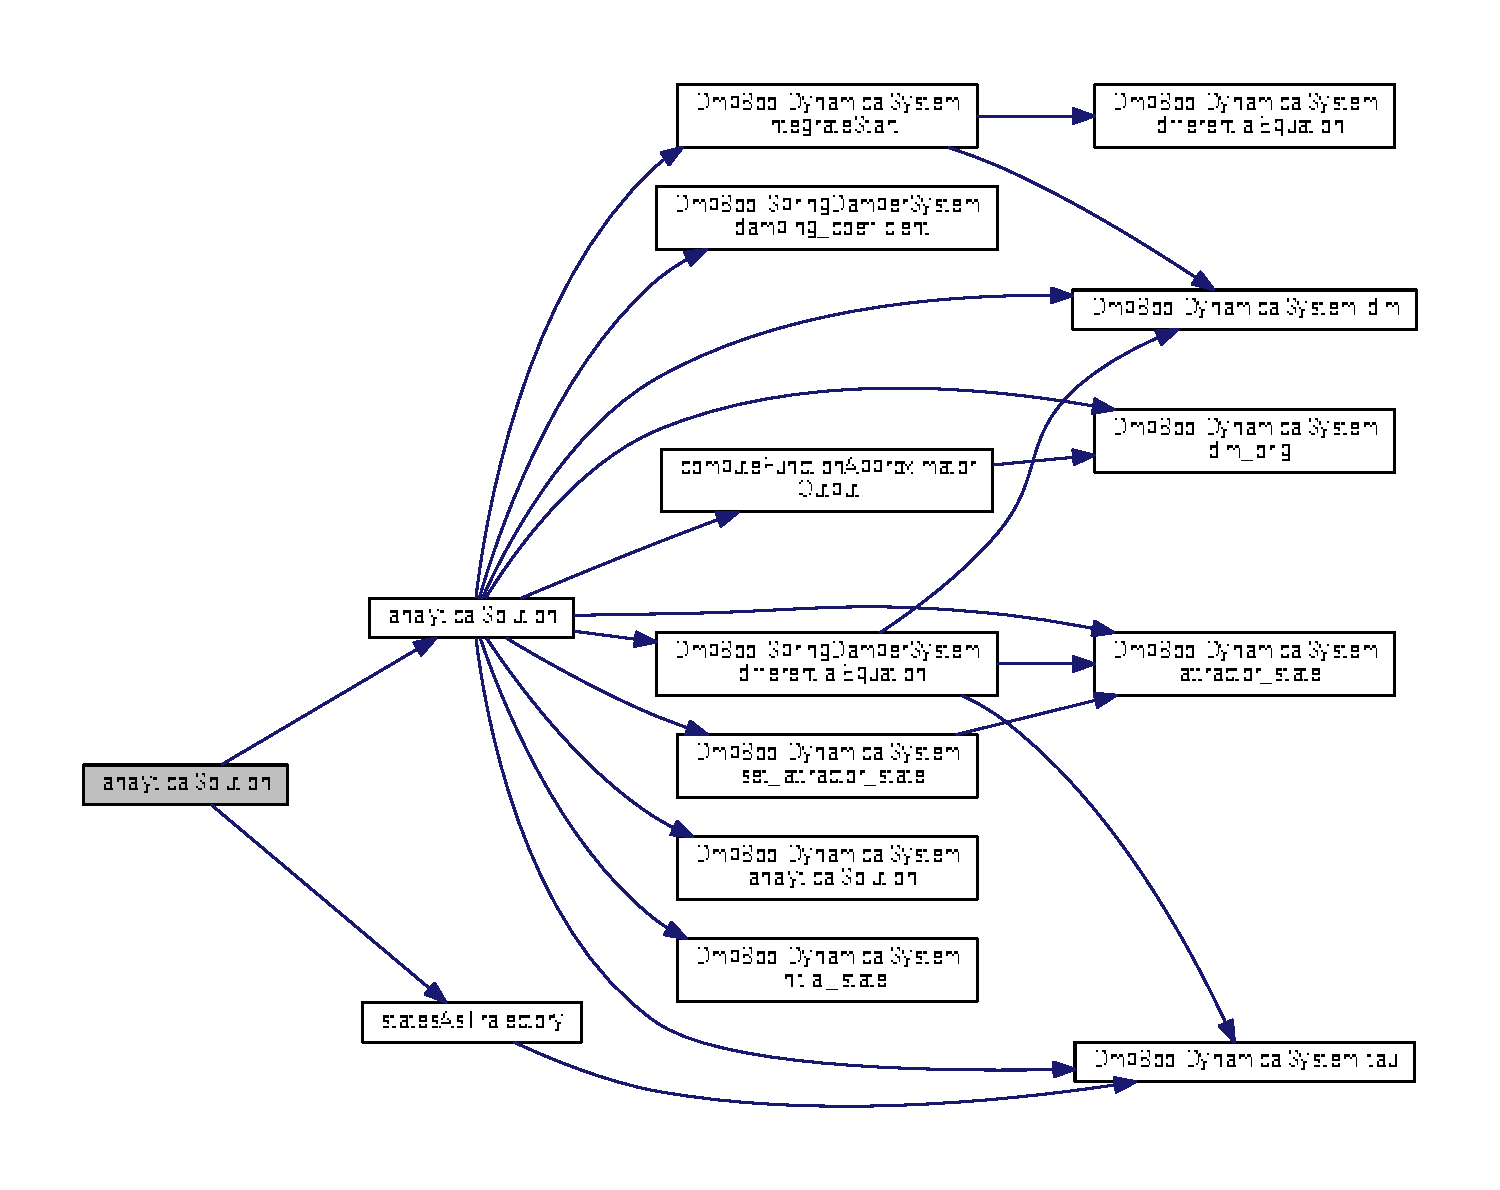
\includegraphics[width=350pt]{classDmpBbo_1_1Dmp_ae1e5218e7ebfedf7fb2501dc8af2675f_cgraph}
\end{center}
\end{figure}


\hypertarget{classDmpBbo_1_1Dmp_aa3ad2fc66e8ce09cfa68032a4a5004b9}{\index{Dmp\+Bbo\+::\+Dmp@{Dmp\+Bbo\+::\+Dmp}!states\+As\+Trajectory@{states\+As\+Trajectory}}
\index{states\+As\+Trajectory@{states\+As\+Trajectory}!Dmp\+Bbo\+::\+Dmp@{Dmp\+Bbo\+::\+Dmp}}
\paragraph[{states\+As\+Trajectory}]{\setlength{\rightskip}{0pt plus 5cm}void states\+As\+Trajectory (
\begin{DoxyParamCaption}
\item[{const Eigen\+::\+Matrix\+Xd \&}]{x\+\_\+in, }
\item[{const Eigen\+::\+Matrix\+Xd \&}]{xd\+\_\+in, }
\item[{Eigen\+::\+Matrix\+Xd \&}]{y\+\_\+out, }
\item[{Eigen\+::\+Matrix\+Xd \&}]{yd\+\_\+out, }
\item[{Eigen\+::\+Matrix\+Xd \&}]{ydd\+\_\+out}
\end{DoxyParamCaption}
) const\hspace{0.3cm}{\ttfamily [virtual]}}}\label{classDmpBbo_1_1Dmp_aa3ad2fc66e8ce09cfa68032a4a5004b9}


Get the output of a D\+M\+P dynamical system as a trajectory. 

As a dynamical system, the state vector of a D\+M\+P contains the output of the goal, spring, phase and gating system. What we are most interested in is the output of the spring system. This function extracts that information, and also computes the accelerations of the spring system, which are only stored implicitely in xd\+\_\+in because second order systems are converted to first order systems with expanded state.


\begin{DoxyParams}[1]{Parameters}
\mbox{\tt in}  & {\em x\+\_\+in} & State vector over time (size n\+\_\+time\+\_\+steps X \hyperlink{group__DynamicalSystems_ga6f628f7f4ed9d77bf69f5b8560b98f18}{dim()}) \\
\hline
\mbox{\tt in}  & {\em xd\+\_\+in} & State vector over time (rates of change) \\
\hline
\mbox{\tt out}  & {\em y\+\_\+out} & State vector over time (size n\+\_\+time\+\_\+steps X \hyperlink{group__DynamicalSystems_ga93d7cbbf2e471b00f124e41706405a05}{dim\+\_\+orig()}) \\
\hline
\mbox{\tt out}  & {\em yd\+\_\+out} & State vector over time (rates of change) \\
\hline
\mbox{\tt out}  & {\em ydd\+\_\+out} & State vector over time (rates of change of rates of change) \\
\hline
\end{DoxyParams}


Definition at line 364 of file Dmp.\+cpp.


\begin{DoxyCode}
365 \{
366   \textcolor{keywordtype}{int} n\_time\_steps = x\_in.rows(); 
367   y\_out  = x\_in.SPRINGM\_Y(n\_time\_steps);
368   yd\_out = xd\_in.SPRINGM\_Y(n\_time\_steps);
369   ydd\_out = xd\_in.SPRINGM\_Z(n\_time\_steps)/\hyperlink{group__DynamicalSystems_ga50eec7ad4c9664b5809ace45b22200d5}{tau}();
370   \textcolor{comment}{// MatrixXd z\_out, zd\_out;}
371   \textcolor{comment}{// z\_out  = x\_in.SPRINGM\_Z(n\_time\_steps);}
372   \textcolor{comment}{// zd\_out = xd\_in.SPRINGM\_Z(n\_time\_steps);}
373   \textcolor{comment}{// Divide by tau to go from z to y space}
374   \textcolor{comment}{// yd = z\_out/obj.tau;}
375   \textcolor{comment}{// ydd\_out = zd\_out/tau();}
376 \}
\end{DoxyCode}


Here is the call graph for this function\+:
\nopagebreak
\begin{figure}[H]
\begin{center}
\leavevmode
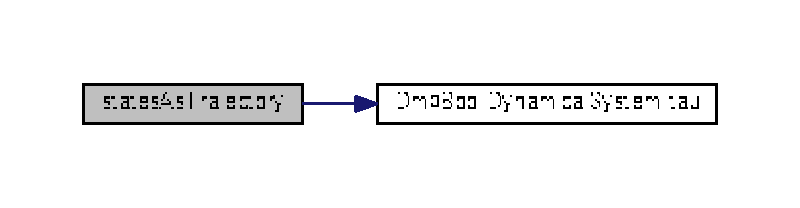
\includegraphics[width=350pt]{classDmpBbo_1_1Dmp_aa3ad2fc66e8ce09cfa68032a4a5004b9_cgraph}
\end{center}
\end{figure}


\hypertarget{classDmpBbo_1_1Dmp_a0a477ccb2da97d3b6f5255a147a0e07c}{\index{Dmp\+Bbo\+::\+Dmp@{Dmp\+Bbo\+::\+Dmp}!states\+As\+Trajectory@{states\+As\+Trajectory}}
\index{states\+As\+Trajectory@{states\+As\+Trajectory}!Dmp\+Bbo\+::\+Dmp@{Dmp\+Bbo\+::\+Dmp}}
\paragraph[{states\+As\+Trajectory}]{\setlength{\rightskip}{0pt plus 5cm}void states\+As\+Trajectory (
\begin{DoxyParamCaption}
\item[{const Eigen\+::\+Vector\+Xd \&}]{ts, }
\item[{const Eigen\+::\+Matrix\+Xd \&}]{x\+\_\+in, }
\item[{const Eigen\+::\+Matrix\+Xd \&}]{xd\+\_\+in, }
\item[{{\bf Trajectory} \&}]{trajectory}
\end{DoxyParamCaption}
) const\hspace{0.3cm}{\ttfamily [virtual]}}}\label{classDmpBbo_1_1Dmp_a0a477ccb2da97d3b6f5255a147a0e07c}


Get the output of a D\+M\+P dynamical system as a trajectory. 

As a dynamical system, the state vector of a D\+M\+P contains the output of the goal, spring, phase and gating system. What we are most interested in is the output of the spring system. This function extracts that information, and also computes the accelerations of the spring system, which are only stored implicitely in xd\+\_\+in because second order systems are converted to first order systems with expanded state.


\begin{DoxyParams}[1]{Parameters}
\mbox{\tt in}  & {\em ts} & A vector of times \\
\hline
\mbox{\tt in}  & {\em x\+\_\+in} & State vector over time \\
\hline
\mbox{\tt in}  & {\em xd\+\_\+in} & State vector over time (rates of change) \\
\hline
\mbox{\tt out}  & {\em trajectory} & \hyperlink{classDmpBbo_1_1Trajectory}{Trajectory} representation of the D\+M\+P state vector output. \\
\hline
\end{DoxyParams}


Definition at line 379 of file Dmp.\+cpp.


\begin{DoxyCode}
379                                                                                                            
                                    \{
380   \textcolor{keywordtype}{int} n\_time\_steps = ts.rows();
381 \textcolor{preprocessor}{#ifndef NDEBUG // Variables below are only required for asserts; check for NDEBUG to avoid warnings.}
382   \textcolor{keywordtype}{int} n\_dims       = x\_in.cols();
383 \textcolor{preprocessor}{#endif}
384   assert(n\_time\_steps==x\_in.rows());
385   assert(n\_time\_steps==xd\_in.rows());
386   assert(n\_dims==xd\_in.cols());
387 
388   \textcolor{comment}{// Left column is time}
389   Trajectory new\_trajectory(
390     ts,
391     \textcolor{comment}{// y\_out (see function above)}
392     x\_in.SPRINGM\_Y(n\_time\_steps),
393     \textcolor{comment}{// yd\_out (see function above)}
394     xd\_in.SPRINGM\_Y(n\_time\_steps),
395     \textcolor{comment}{// ydd\_out (see function above)}
396     xd\_in.SPRINGM\_Z(n\_time\_steps)/\hyperlink{group__DynamicalSystems_ga50eec7ad4c9664b5809ace45b22200d5}{tau}()
397   );
398   
399   trajectory = new\_trajectory;
400   
401 \}
\end{DoxyCode}


Here is the call graph for this function\+:
\nopagebreak
\begin{figure}[H]
\begin{center}
\leavevmode
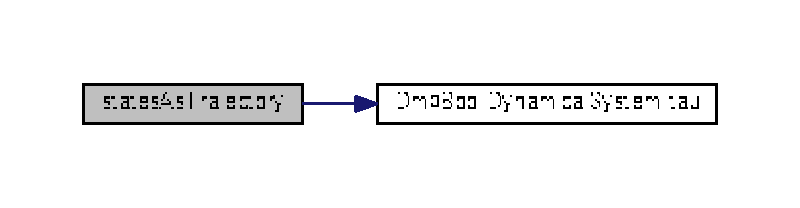
\includegraphics[width=350pt]{classDmpBbo_1_1Dmp_a0a477ccb2da97d3b6f5255a147a0e07c_cgraph}
\end{center}
\end{figure}


\hypertarget{classDmpBbo_1_1Dmp_a5d14dedc6736ec5675b4026437b8a597}{\index{Dmp\+Bbo\+::\+Dmp@{Dmp\+Bbo\+::\+Dmp}!train@{train}}
\index{train@{train}!Dmp\+Bbo\+::\+Dmp@{Dmp\+Bbo\+::\+Dmp}}
\paragraph[{train}]{\setlength{\rightskip}{0pt plus 5cm}void train (
\begin{DoxyParamCaption}
\item[{const {\bf Trajectory} \&}]{trajectory}
\end{DoxyParamCaption}
)}}\label{classDmpBbo_1_1Dmp_a5d14dedc6736ec5675b4026437b8a597}


Train a D\+M\+P with a trajectory. 


\begin{DoxyParams}[1]{Parameters}
\mbox{\tt in}  & {\em trajectory} & The trajectory with which to train the D\+M\+P. \\
\hline
\end{DoxyParams}


Definition at line 564 of file Dmp.\+cpp.


\begin{DoxyCode}
565 \{
566   \hyperlink{classDmpBbo_1_1Dmp_a5d14dedc6736ec5675b4026437b8a597}{train}(trajectory,\textcolor{stringliteral}{""});
567 \}
\end{DoxyCode}
\hypertarget{classDmpBbo_1_1Dmp_abca46c9155c3cfbc71d10aabdcf3384c}{\index{Dmp\+Bbo\+::\+Dmp@{Dmp\+Bbo\+::\+Dmp}!train@{train}}
\index{train@{train}!Dmp\+Bbo\+::\+Dmp@{Dmp\+Bbo\+::\+Dmp}}
\paragraph[{train}]{\setlength{\rightskip}{0pt plus 5cm}void train (
\begin{DoxyParamCaption}
\item[{const {\bf Trajectory} \&}]{trajectory, }
\item[{std\+::string}]{save\+\_\+directory, }
\item[{bool}]{overwrite = {\ttfamily false}}
\end{DoxyParamCaption}
)}}\label{classDmpBbo_1_1Dmp_abca46c9155c3cfbc71d10aabdcf3384c}


Train a D\+M\+P with a trajectory, and write results to file. 


\begin{DoxyParams}[1]{Parameters}
\mbox{\tt in}  & {\em trajectory} & The trajectory with which to train the D\+M\+P. \\
\hline
\mbox{\tt in}  & {\em save\+\_\+directory} & The directory to which to save the results. \\
\hline
\mbox{\tt in}  & {\em overwrite} & Overwrite existing files in the directory above (default\+: false) \\
\hline
\end{DoxyParams}


Definition at line 569 of file Dmp.\+cpp.


\begin{DoxyCode}
570 \{
571   
572   \textcolor{comment}{// Set tau, initial\_state and attractor\_state from the trajectory }
573   \hyperlink{classDmpBbo_1_1Dmp_a17edb45ef62a4ef7f8c78e4f8f68b249}{set\_tau}(trajectory.duration());
574   \hyperlink{classDmpBbo_1_1Dmp_ad4e11c676c2add8a992db1caf542f0a0}{set\_initial\_state}(trajectory.initial\_y());
575   \hyperlink{classDmpBbo_1_1Dmp_a6dccbd077acfd148f528a48a72a4003f}{set\_attractor\_state}(trajectory.final\_y());
576   
577   VectorXd fa\_input\_phase;
578   MatrixXd f\_target;
579   \hyperlink{classDmpBbo_1_1Dmp_a9aef6cbf41e55caa12b62cff77cf1fda}{computeFunctionApproximatorInputsAndTargets}(trajectory, 
      fa\_input\_phase, f\_target);
580   
581   \textcolor{comment}{// Some checks before training function approximators}
582   assert(!function\_approximators\_.empty());
583   
584   \textcolor{keywordflow}{for} (\textcolor{keywordtype}{unsigned} \textcolor{keywordtype}{int} dd=0; dd<function\_approximators\_.size(); dd++)
585   \{
586     \textcolor{comment}{// This is just boring stuff to figure out if and where to store the results of training}
587     \textcolor{keywordtype}{string} save\_directory\_dim;
588     \textcolor{keywordflow}{if} (!save\_directory.empty())
589     \{
590       \textcolor{keywordflow}{if} (function\_approximators\_.size()==1)
591         save\_directory\_dim = save\_directory;
592       \textcolor{keywordflow}{else}
593         save\_directory\_dim = save\_directory + \textcolor{stringliteral}{"/dim"} + to\_string(dd);
594     \}
595     
596     \textcolor{comment}{// Actual training is happening here.}
597     VectorXd fa\_target = f\_target.col(dd);
598     \textcolor{keywordflow}{if} (function\_approximators\_[dd]==NULL)
599     \{
600       cerr << \_\_FILE\_\_ << \textcolor{stringliteral}{":"} << \_\_LINE\_\_ << \textcolor{stringliteral}{":"};
601       cerr << \textcolor{stringliteral}{"WARNING: function approximator cannot be trained because it is NULL."} << endl;
602     \}
603     \textcolor{keywordflow}{else}
604     \{
605       \textcolor{keywordflow}{if} (function\_approximators\_[dd]->isTrained())
606         function\_approximators\_[dd]->reTrain(fa\_input\_phase,fa\_target,save\_directory\_dim,overwrite);
607       \textcolor{keywordflow}{else}
608         function\_approximators\_[dd]->train(fa\_input\_phase,fa\_target,save\_directory\_dim,overwrite);
609     \}
610   \}
611 \}
\end{DoxyCode}


Here is the call graph for this function\+:
\nopagebreak
\begin{figure}[H]
\begin{center}
\leavevmode
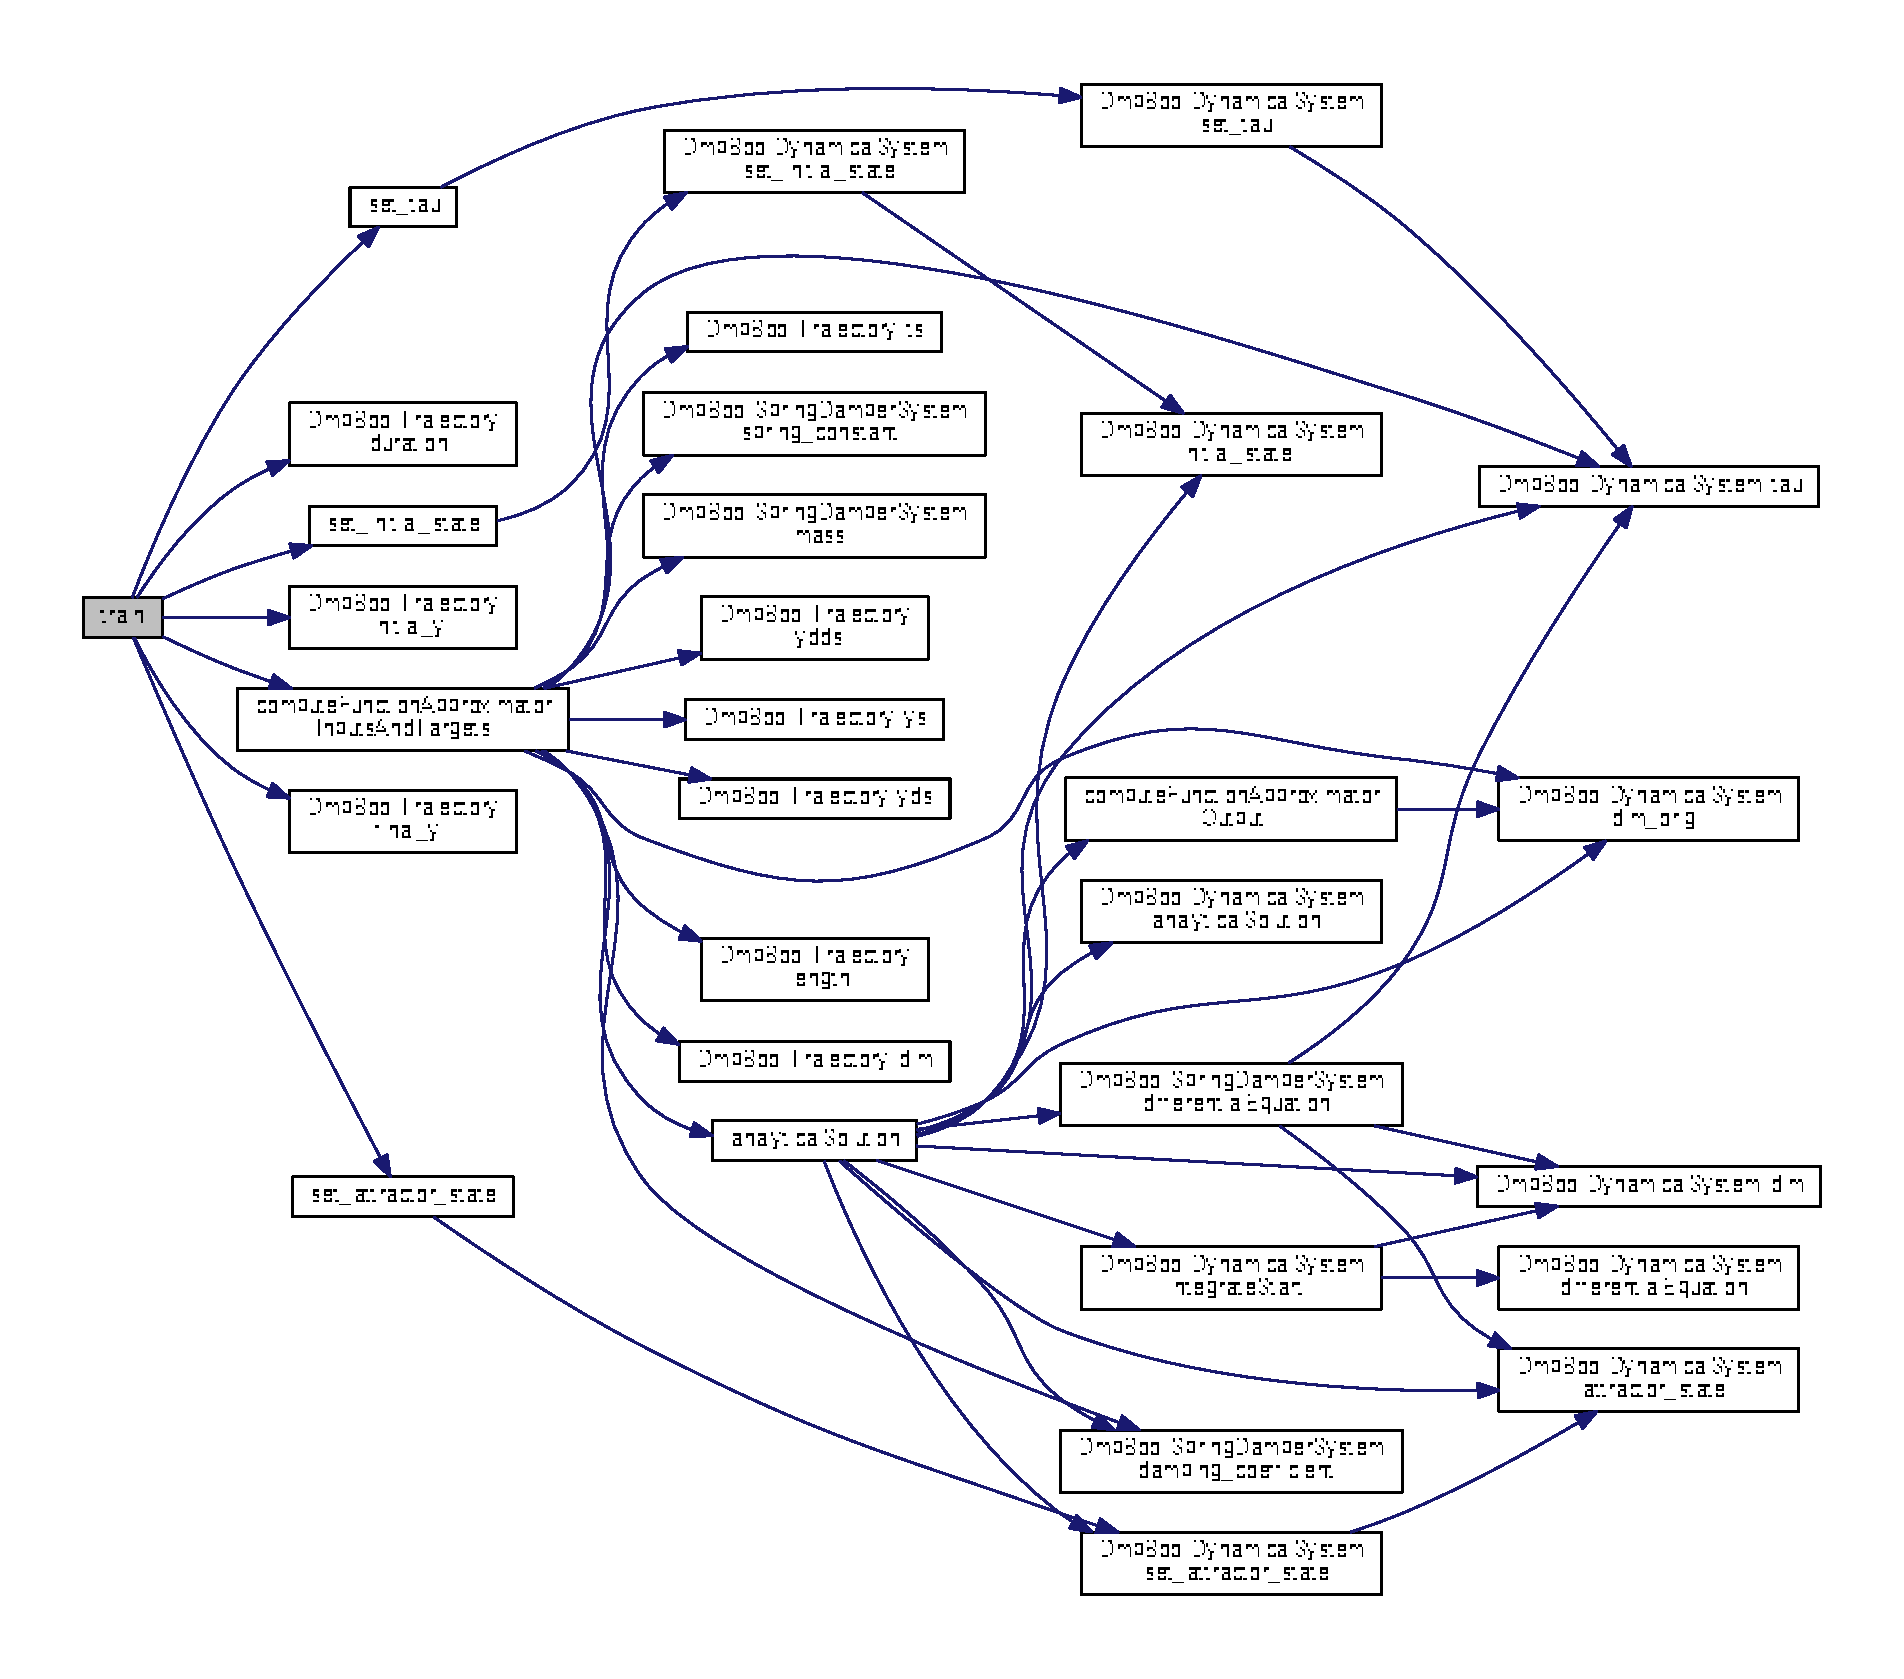
\includegraphics[width=350pt]{classDmpBbo_1_1Dmp_abca46c9155c3cfbc71d10aabdcf3384c_cgraph}
\end{center}
\end{figure}


\hypertarget{classDmpBbo_1_1Dmp_a17edb45ef62a4ef7f8c78e4f8f68b249}{\index{Dmp\+Bbo\+::\+Dmp@{Dmp\+Bbo\+::\+Dmp}!set\+\_\+tau@{set\+\_\+tau}}
\index{set\+\_\+tau@{set\+\_\+tau}!Dmp\+Bbo\+::\+Dmp@{Dmp\+Bbo\+::\+Dmp}}
\paragraph[{set\+\_\+tau}]{\setlength{\rightskip}{0pt plus 5cm}void set\+\_\+tau (
\begin{DoxyParamCaption}
\item[{double}]{tau}
\end{DoxyParamCaption}
)\hspace{0.3cm}{\ttfamily [virtual]}}}\label{classDmpBbo_1_1Dmp_a17edb45ef62a4ef7f8c78e4f8f68b249}


Accessor function for the time constant. 


\begin{DoxyParams}[1]{Parameters}
\mbox{\tt in}  & {\em tau} & Time constant We need to override \hyperlink{group__DynamicalSystems_ga91155da280310b176cbd5fc1627820c7}{Dynamical\+System\+::set\+\_\+tau}, because the D\+M\+P must also change the time constant of all of its subsystems. \\
\hline
\end{DoxyParams}


Reimplemented from \hyperlink{group__DynamicalSystems_ga91155da280310b176cbd5fc1627820c7}{Dynamical\+System}.



Definition at line 758 of file Dmp.\+cpp.


\begin{DoxyCode}
758                             \{
759   \hyperlink{group__DynamicalSystems_ga91155da280310b176cbd5fc1627820c7}{DynamicalSystem::set\_tau}(\hyperlink{group__DynamicalSystems_ga50eec7ad4c9664b5809ace45b22200d5}{tau});
760 
761   \textcolor{comment}{// Set value in all relevant subsystems also  }
762   spring\_system\_->\hyperlink{group__DynamicalSystems_ga91155da280310b176cbd5fc1627820c7}{set\_tau}(\hyperlink{group__DynamicalSystems_ga50eec7ad4c9664b5809ace45b22200d5}{tau});
763   \textcolor{keywordflow}{if} (goal\_system\_!=NULL)
764     goal\_system\_->\hyperlink{group__DynamicalSystems_ga91155da280310b176cbd5fc1627820c7}{set\_tau}(\hyperlink{group__DynamicalSystems_ga50eec7ad4c9664b5809ace45b22200d5}{tau});
765   phase\_system\_ ->\hyperlink{group__DynamicalSystems_ga91155da280310b176cbd5fc1627820c7}{set\_tau}(\hyperlink{group__DynamicalSystems_ga50eec7ad4c9664b5809ace45b22200d5}{tau});
766   gating\_system\_->\hyperlink{group__DynamicalSystems_ga91155da280310b176cbd5fc1627820c7}{set\_tau}(\hyperlink{group__DynamicalSystems_ga50eec7ad4c9664b5809ace45b22200d5}{tau});
767 \}
\end{DoxyCode}


Here is the call graph for this function\+:
\nopagebreak
\begin{figure}[H]
\begin{center}
\leavevmode
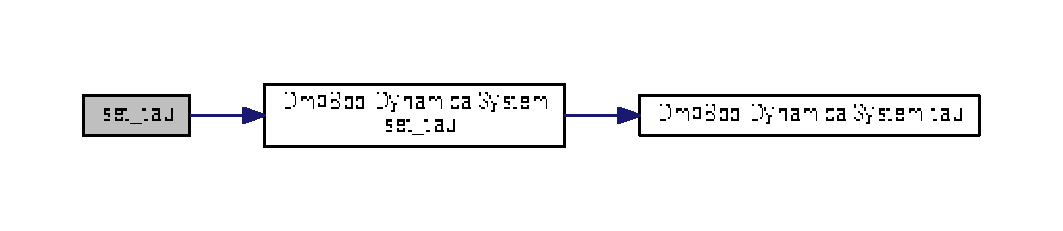
\includegraphics[width=350pt]{classDmpBbo_1_1Dmp_a17edb45ef62a4ef7f8c78e4f8f68b249_cgraph}
\end{center}
\end{figure}


\hypertarget{classDmpBbo_1_1Dmp_ad4e11c676c2add8a992db1caf542f0a0}{\index{Dmp\+Bbo\+::\+Dmp@{Dmp\+Bbo\+::\+Dmp}!set\+\_\+initial\+\_\+state@{set\+\_\+initial\+\_\+state}}
\index{set\+\_\+initial\+\_\+state@{set\+\_\+initial\+\_\+state}!Dmp\+Bbo\+::\+Dmp@{Dmp\+Bbo\+::\+Dmp}}
\paragraph[{set\+\_\+initial\+\_\+state}]{\setlength{\rightskip}{0pt plus 5cm}void set\+\_\+initial\+\_\+state (
\begin{DoxyParamCaption}
\item[{const Eigen\+::\+Vector\+Xd \&}]{y\+\_\+init}
\end{DoxyParamCaption}
)\hspace{0.3cm}{\ttfamily [virtual]}}}\label{classDmpBbo_1_1Dmp_ad4e11c676c2add8a992db1caf542f0a0}


Accessor function for the initial state of the system. 


\begin{DoxyParams}[1]{Parameters}
\mbox{\tt in}  & {\em y\+\_\+init} & Initial state of the system. We need to override \hyperlink{group__DynamicalSystems_ga23f05bcccb6a5deda6d2a5364d8ebb16}{Dynamical\+System\+::set\+\_\+initial\+\_\+state}, because the D\+M\+P must also change the initial state of the goal system as well. \\
\hline
\end{DoxyParams}


Reimplemented from \hyperlink{group__DynamicalSystems_ga23f05bcccb6a5deda6d2a5364d8ebb16}{Dynamical\+System}.



Definition at line 769 of file Dmp.\+cpp.


\begin{DoxyCode}
769                                                   \{
770   \hyperlink{group__DynamicalSystems_ga23f05bcccb6a5deda6d2a5364d8ebb16}{DynamicalSystem::set\_initial\_state}(y\_init);
771   
772   \textcolor{comment}{// Set value in all relevant subsystems also  }
773   spring\_system\_->\hyperlink{group__DynamicalSystems_ga23f05bcccb6a5deda6d2a5364d8ebb16}{set\_initial\_state}(y\_init);
774   \textcolor{keywordflow}{if} (goal\_system\_!=NULL)
775     goal\_system\_->\hyperlink{group__DynamicalSystems_ga23f05bcccb6a5deda6d2a5364d8ebb16}{set\_initial\_state}(y\_init);
776 \}    
\end{DoxyCode}


Here is the call graph for this function\+:
\nopagebreak
\begin{figure}[H]
\begin{center}
\leavevmode
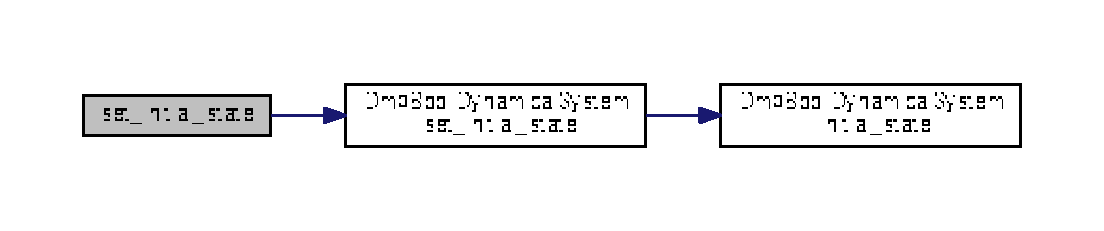
\includegraphics[width=350pt]{classDmpBbo_1_1Dmp_ad4e11c676c2add8a992db1caf542f0a0_cgraph}
\end{center}
\end{figure}


\hypertarget{classDmpBbo_1_1Dmp_a6dccbd077acfd148f528a48a72a4003f}{\index{Dmp\+Bbo\+::\+Dmp@{Dmp\+Bbo\+::\+Dmp}!set\+\_\+attractor\+\_\+state@{set\+\_\+attractor\+\_\+state}}
\index{set\+\_\+attractor\+\_\+state@{set\+\_\+attractor\+\_\+state}!Dmp\+Bbo\+::\+Dmp@{Dmp\+Bbo\+::\+Dmp}}
\paragraph[{set\+\_\+attractor\+\_\+state}]{\setlength{\rightskip}{0pt plus 5cm}void set\+\_\+attractor\+\_\+state (
\begin{DoxyParamCaption}
\item[{const Eigen\+::\+Vector\+Xd \&}]{y\+\_\+attr}
\end{DoxyParamCaption}
)\hspace{0.3cm}{\ttfamily [virtual]}}}\label{classDmpBbo_1_1Dmp_a6dccbd077acfd148f528a48a72a4003f}


Accessor function for the attractor state of the system. 


\begin{DoxyParams}[1]{Parameters}
\mbox{\tt in}  & {\em y\+\_\+attr} & Attractor state of the system. \\
\hline
\end{DoxyParams}


Reimplemented from \hyperlink{group__DynamicalSystems_ga32a975e60b5f001308368c7f06b90e18}{Dynamical\+System}.



Definition at line 778 of file Dmp.\+cpp.


\begin{DoxyCode}
778                                                     \{
779   \hyperlink{group__DynamicalSystems_ga32a975e60b5f001308368c7f06b90e18}{DynamicalSystem::set\_attractor\_state}(y\_attr);
780   
781   \textcolor{comment}{// Set value in all relevant subsystems also  }
782   \textcolor{keywordflow}{if} (goal\_system\_!=NULL)
783     goal\_system\_->\hyperlink{group__DynamicalSystems_ga32a975e60b5f001308368c7f06b90e18}{set\_attractor\_state}(y\_attr);
784 
785   \textcolor{comment}{// Do NOT do the following. The attractor state of the spring system is determined by the goal }
786   \textcolor{comment}{// system}
787   \textcolor{comment}{// spring\_system\_->set\_attractor\_state(y\_attr);}
788 
789 \}    
\end{DoxyCode}


Here is the call graph for this function\+:
\nopagebreak
\begin{figure}[H]
\begin{center}
\leavevmode
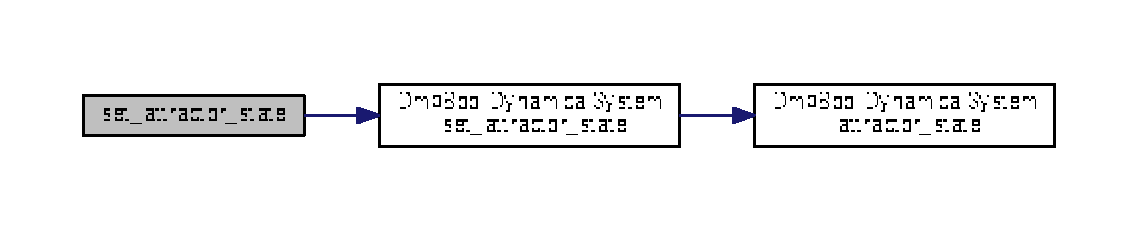
\includegraphics[width=350pt]{classDmpBbo_1_1Dmp_a6dccbd077acfd148f528a48a72a4003f_cgraph}
\end{center}
\end{figure}


\hypertarget{classDmpBbo_1_1Dmp_a0b6f58851f4a8fc8b433936cff4c3e7e}{\index{Dmp\+Bbo\+::\+Dmp@{Dmp\+Bbo\+::\+Dmp}!set\+\_\+damping\+\_\+coefficient@{set\+\_\+damping\+\_\+coefficient}}
\index{set\+\_\+damping\+\_\+coefficient@{set\+\_\+damping\+\_\+coefficient}!Dmp\+Bbo\+::\+Dmp@{Dmp\+Bbo\+::\+Dmp}}
\paragraph[{set\+\_\+damping\+\_\+coefficient}]{\setlength{\rightskip}{0pt plus 5cm}void set\+\_\+damping\+\_\+coefficient (
\begin{DoxyParamCaption}
\item[{double}]{damping\+\_\+coefficient}
\end{DoxyParamCaption}
)}}\label{classDmpBbo_1_1Dmp_a0b6f58851f4a8fc8b433936cff4c3e7e}


Accessor function for damping coefficient of spring-\/damper system. 


\begin{DoxyParams}[1]{Parameters}
\mbox{\tt in}  & {\em damping\+\_\+coefficient} & Damping coefficient \\
\hline
\end{DoxyParams}


Definition at line 200 of file Dmp.\+cpp.


\begin{DoxyCode}
201 \{
202   spring\_system\_->\hyperlink{classDmpBbo_1_1SpringDamperSystem_a0b6f58851f4a8fc8b433936cff4c3e7e}{set\_damping\_coefficient}(damping\_coefficient); 
203 \}
\end{DoxyCode}


Here is the call graph for this function\+:
\nopagebreak
\begin{figure}[H]
\begin{center}
\leavevmode
\includegraphics[width=350pt]{classDmpBbo_1_1Dmp_a0b6f58851f4a8fc8b433936cff4c3e7e_cgraph}
\end{center}
\end{figure}


\hypertarget{classDmpBbo_1_1Dmp_a8844968245473d1fedd2a2b632fb074a}{\index{Dmp\+Bbo\+::\+Dmp@{Dmp\+Bbo\+::\+Dmp}!set\+\_\+spring\+\_\+constant@{set\+\_\+spring\+\_\+constant}}
\index{set\+\_\+spring\+\_\+constant@{set\+\_\+spring\+\_\+constant}!Dmp\+Bbo\+::\+Dmp@{Dmp\+Bbo\+::\+Dmp}}
\paragraph[{set\+\_\+spring\+\_\+constant}]{\setlength{\rightskip}{0pt plus 5cm}void set\+\_\+spring\+\_\+constant (
\begin{DoxyParamCaption}
\item[{double}]{spring\+\_\+constant}
\end{DoxyParamCaption}
)}}\label{classDmpBbo_1_1Dmp_a8844968245473d1fedd2a2b632fb074a}


Accessor function for spring constant of spring-\/damper system. 


\begin{DoxyParams}[1]{Parameters}
\mbox{\tt in}  & {\em spring\+\_\+constant} & Spring constant \\
\hline
\end{DoxyParams}


Definition at line 204 of file Dmp.\+cpp.


\begin{DoxyCode}
204                                                     \{
205   spring\_system\_->\hyperlink{classDmpBbo_1_1SpringDamperSystem_a8844968245473d1fedd2a2b632fb074a}{set\_spring\_constant}(spring\_constant); 
206 \}
\end{DoxyCode}


Here is the call graph for this function\+:
\nopagebreak
\begin{figure}[H]
\begin{center}
\leavevmode
\includegraphics[width=350pt]{classDmpBbo_1_1Dmp_a8844968245473d1fedd2a2b632fb074a_cgraph}
\end{center}
\end{figure}


\hypertarget{classDmpBbo_1_1Dmp_a1aca816b42cf0d36118be0ab91120d77}{\index{Dmp\+Bbo\+::\+Dmp@{Dmp\+Bbo\+::\+Dmp}!to\+String@{to\+String}}
\index{to\+String@{to\+String}!Dmp\+Bbo\+::\+Dmp@{Dmp\+Bbo\+::\+Dmp}}
\paragraph[{to\+String}]{\setlength{\rightskip}{0pt plus 5cm}string to\+String (
\begin{DoxyParamCaption}
\item[{void}]{}
\end{DoxyParamCaption}
) const\hspace{0.3cm}{\ttfamily [virtual]}}}\label{classDmpBbo_1_1Dmp_a1aca816b42cf0d36118be0ab91120d77}


Returns a string representation of the object. 

\begin{DoxyReturn}{Returns}
A string representation of the object. 
\end{DoxyReturn}


Implements \hyperlink{classDmpBbo_1_1DynamicalSystem_af084bff2ddd6233e9a898faa23f6195c}{Dynamical\+System}.



Definition at line 792 of file Dmp.\+cpp.


\begin{DoxyCode}
793 \{
794   \hyperlink{BoostSerializationToString_8hpp_a244fa2647b6577d9be517958dccbb5e8}{RETURN\_STRING\_FROM\_BOOST\_SERIALIZATION\_XML}(\textcolor{stringliteral}{"Dmp"});
795 \}
\end{DoxyCode}
\hypertarget{classDmpBbo_1_1Dmp_adaae949509cd3b2e6ce58deb841c80a0}{\index{Dmp\+Bbo\+::\+Dmp@{Dmp\+Bbo\+::\+Dmp}!get\+Selectable\+Parameters@{get\+Selectable\+Parameters}}
\index{get\+Selectable\+Parameters@{get\+Selectable\+Parameters}!Dmp\+Bbo\+::\+Dmp@{Dmp\+Bbo\+::\+Dmp}}
\paragraph[{get\+Selectable\+Parameters}]{\setlength{\rightskip}{0pt plus 5cm}void get\+Selectable\+Parameters (
\begin{DoxyParamCaption}
\item[{std\+::set$<$ std\+::string $>$ \&}]{selected\+\_\+values\+\_\+labels}
\end{DoxyParamCaption}
) const\hspace{0.3cm}{\ttfamily [virtual]}}}\label{classDmpBbo_1_1Dmp_adaae949509cd3b2e6ce58deb841c80a0}


Return all the names of the parameter types that can be selected. 


\begin{DoxyParams}[1]{Parameters}
\mbox{\tt out}  & {\em selected\+\_\+values\+\_\+labels} & Names of the parameter types that can be selected \\
\hline
\end{DoxyParams}


Implements \hyperlink{classDmpBbo_1_1Parameterizable_ac378b5f6e435af19251fb6537ba30ade}{Parameterizable}.



Definition at line 613 of file Dmp.\+cpp.


\begin{DoxyCode}
613                                                                              \{
614   assert(function\_approximators\_.size()>0);
615   \textcolor{keywordflow}{for} (\textcolor{keywordtype}{int} dd=0; dd<\hyperlink{group__DynamicalSystems_ga93d7cbbf2e471b00f124e41706405a05}{dim\_orig}(); dd++)
616   \{
617     \textcolor{keywordflow}{if} (function\_approximators\_[dd]!=NULL)
618     \{
619       \textcolor{keywordflow}{if} (function\_approximators\_[dd]->isTrained())
620       \{
621         set<string> cur\_labels;
622         function\_approximators\_[dd]->getSelectableParameters(cur\_labels);
623         selectable\_values\_labels.insert(cur\_labels.begin(), cur\_labels.end());
624       \}
625     \}
626   \}
627   selectable\_values\_labels.insert(\textcolor{stringliteral}{"goal"});
628   
629   \textcolor{comment}{//cout << "selected\_values\_labels=["; }
630   \textcolor{comment}{//for (string label : selected\_values\_labels) }
631   \textcolor{comment}{//  cout << label << " ";}
632   \textcolor{comment}{//cout << "]" << endl;}
633   
634 \}
\end{DoxyCode}


Here is the call graph for this function\+:
\nopagebreak
\begin{figure}[H]
\begin{center}
\leavevmode
\includegraphics[width=350pt]{classDmpBbo_1_1Dmp_adaae949509cd3b2e6ce58deb841c80a0_cgraph}
\end{center}
\end{figure}


\hypertarget{classDmpBbo_1_1Dmp_a8a976b5db2d1809ece10e431816f0f27}{\index{Dmp\+Bbo\+::\+Dmp@{Dmp\+Bbo\+::\+Dmp}!set\+Selected\+Parameters@{set\+Selected\+Parameters}}
\index{set\+Selected\+Parameters@{set\+Selected\+Parameters}!Dmp\+Bbo\+::\+Dmp@{Dmp\+Bbo\+::\+Dmp}}
\paragraph[{set\+Selected\+Parameters}]{\setlength{\rightskip}{0pt plus 5cm}void set\+Selected\+Parameters (
\begin{DoxyParamCaption}
\item[{const std\+::set$<$ std\+::string $>$ \&}]{selected\+\_\+values\+\_\+labels}
\end{DoxyParamCaption}
)\hspace{0.3cm}{\ttfamily [virtual]}}}\label{classDmpBbo_1_1Dmp_a8a976b5db2d1809ece10e431816f0f27}


Determine which subset of parameters is represented in the vector returned by \hyperlink{classDmpBbo_1_1Parameterizable_aab955bec57f074a991b8be31d6ce54ca}{Parameterizable\+::get\+Parameter\+Vector\+Selected}. 

Different function approximators have different types of model parameters. For instance, L\+W\+R has the centers and widths of basis functions, along with the slopes of each line segment. \hyperlink{classDmpBbo_1_1Parameterizable_a8a976b5db2d1809ece10e431816f0f27}{Parameterizable\+::set\+Selected\+Parameters} provides a means to determine which parameters should be returned by \hyperlink{classDmpBbo_1_1Parameterizable_aab955bec57f074a991b8be31d6ce54ca}{Parameterizable\+::get\+Parameter\+Vector\+Selected}, i.\+e. by calling\+: std\+::set$<$std\+::string$>$ selected; selected.\+insert(\char`\"{}slopes\char`\"{}); model\+\_\+parameters.\+set\+Selected\+Parameters(selected) 
\begin{DoxyParams}[1]{Parameters}
\mbox{\tt in}  & {\em selected\+\_\+values\+\_\+labels} & The names of the parameters that are selected \\
\hline
\end{DoxyParams}


Reimplemented from \hyperlink{classDmpBbo_1_1Parameterizable_a8a976b5db2d1809ece10e431816f0f27}{Parameterizable}.



Definition at line 636 of file Dmp.\+cpp.


\begin{DoxyCode}
637 \{
638   assert(function\_approximators\_.size()>0);
639   \textcolor{keywordflow}{for} (\textcolor{keywordtype}{int} dd=0; dd<\hyperlink{group__DynamicalSystems_ga93d7cbbf2e471b00f124e41706405a05}{dim\_orig}(); dd++)
640     \textcolor{keywordflow}{if} (function\_approximators\_[dd]!=NULL)
641       \textcolor{keywordflow}{if} (function\_approximators\_[dd]->isTrained())
642         function\_approximators\_[dd]->\hyperlink{classDmpBbo_1_1Dmp_a8a976b5db2d1809ece10e431816f0f27}{setSelectedParameters}(selected\_values\_labels);
643 
644   \textcolor{comment}{// Call superclass for initializations}
645   \hyperlink{classDmpBbo_1_1Parameterizable_a8a976b5db2d1809ece10e431816f0f27}{Parameterizable::setSelectedParameters}(selected\_values\_labels);
646 
647   VectorXi lengths\_per\_dimension = VectorXi::Zero(\hyperlink{group__DynamicalSystems_ga93d7cbbf2e471b00f124e41706405a05}{dim\_orig}());
648   \textcolor{keywordflow}{for} (\textcolor{keywordtype}{int} dd=0; dd<\hyperlink{group__DynamicalSystems_ga93d7cbbf2e471b00f124e41706405a05}{dim\_orig}(); dd++)
649   \{
650     \textcolor{keywordflow}{if} (function\_approximators\_[dd]!=NULL)
651       \textcolor{keywordflow}{if} (function\_approximators\_[dd]->isTrained())
652         lengths\_per\_dimension[dd] = function\_approximators\_[dd]->
      \hyperlink{classDmpBbo_1_1Parameterizable_ae83cb950bcf5219841e6ca8511ac2907}{getParameterVectorSelectedSize}();
653     
654     \textcolor{keywordflow}{if} (selected\_values\_labels.find(\textcolor{stringliteral}{"goal"})!=selected\_values\_labels.end())
655       lengths\_per\_dimension[dd]++;
656   \}
657   
658   \hyperlink{classDmpBbo_1_1Parameterizable_a77089aa6cc3b95dd0a1c17de7bc033b9}{setVectorLengthsPerDimension}(lengths\_per\_dimension);
659       
660 \}
\end{DoxyCode}


Here is the call graph for this function\+:
\nopagebreak
\begin{figure}[H]
\begin{center}
\leavevmode
\includegraphics[width=350pt]{classDmpBbo_1_1Dmp_a8a976b5db2d1809ece10e431816f0f27_cgraph}
\end{center}
\end{figure}


\hypertarget{classDmpBbo_1_1Dmp_ab24d2485b3b795b516f4844f225100eb}{\index{Dmp\+Bbo\+::\+Dmp@{Dmp\+Bbo\+::\+Dmp}!get\+Parameter\+Vector\+All\+Size@{get\+Parameter\+Vector\+All\+Size}}
\index{get\+Parameter\+Vector\+All\+Size@{get\+Parameter\+Vector\+All\+Size}!Dmp\+Bbo\+::\+Dmp@{Dmp\+Bbo\+::\+Dmp}}
\paragraph[{get\+Parameter\+Vector\+All\+Size}]{\setlength{\rightskip}{0pt plus 5cm}int get\+Parameter\+Vector\+All\+Size (
\begin{DoxyParamCaption}
\item[{void}]{}
\end{DoxyParamCaption}
) const\hspace{0.3cm}{\ttfamily [virtual]}}}\label{classDmpBbo_1_1Dmp_ab24d2485b3b795b516f4844f225100eb}


Get the size of the parameter values vector when it contains all available parameter values. 

\begin{DoxyReturn}{Returns}
The size of the parameter vector
\end{DoxyReturn}
For instance, if the parameters consists of centers, widths and slopes the parameter values vector will be something like \begin{DoxyVerb}    centers     widths    slopes
[ 100 110 120 10 10 10 0.4 0.7 0.4 ]
\end{DoxyVerb}
 then \hyperlink{classDmpBbo_1_1Dmp_ab24d2485b3b795b516f4844f225100eb}{get\+Parameter\+Vector\+All\+Size()} will return 9 

Implements \hyperlink{classDmpBbo_1_1Parameterizable_ab89eda9a1c1ba010db81002975e6e52c}{Parameterizable}.



Definition at line 706 of file Dmp.\+cpp.


\begin{DoxyCode}
707 \{
708   \textcolor{keywordtype}{int} total\_size = 0;
709   \textcolor{keywordflow}{for} (\textcolor{keywordtype}{unsigned} \textcolor{keywordtype}{int} dd=0; dd<function\_approximators\_.size(); dd++)
710     total\_size += function\_approximators\_[dd]->\hyperlink{classDmpBbo_1_1Dmp_ab24d2485b3b795b516f4844f225100eb}{getParameterVectorAllSize}();
711   
712   \textcolor{comment}{// For the goal}
713   total\_size += \hyperlink{group__DynamicalSystems_ga93d7cbbf2e471b00f124e41706405a05}{dim\_orig}();
714   \textcolor{keywordflow}{return} total\_size;
715 \}
\end{DoxyCode}


Here is the call graph for this function\+:
\nopagebreak
\begin{figure}[H]
\begin{center}
\leavevmode
\includegraphics[width=350pt]{classDmpBbo_1_1Dmp_ab24d2485b3b795b516f4844f225100eb_cgraph}
\end{center}
\end{figure}


\hypertarget{classDmpBbo_1_1Dmp_ac44b51e5335f973eed54f100618e5496}{\index{Dmp\+Bbo\+::\+Dmp@{Dmp\+Bbo\+::\+Dmp}!get\+Parameter\+Vector\+All@{get\+Parameter\+Vector\+All}}
\index{get\+Parameter\+Vector\+All@{get\+Parameter\+Vector\+All}!Dmp\+Bbo\+::\+Dmp@{Dmp\+Bbo\+::\+Dmp}}
\paragraph[{get\+Parameter\+Vector\+All}]{\setlength{\rightskip}{0pt plus 5cm}void get\+Parameter\+Vector\+All (
\begin{DoxyParamCaption}
\item[{Eigen\+::\+Vector\+Xd \&}]{values}
\end{DoxyParamCaption}
) const\hspace{0.3cm}{\ttfamily [virtual]}}}\label{classDmpBbo_1_1Dmp_ac44b51e5335f973eed54f100618e5496}


Return a vector that returns all available parameter values. 


\begin{DoxyParams}[1]{Parameters}
\mbox{\tt out}  & {\em values} & All available parameter values in one vector. \\
\hline
\end{DoxyParams}
\begin{DoxyRemark}{Remarks}
Contrast this with \hyperlink{classDmpBbo_1_1Parameterizable_aab955bec57f074a991b8be31d6ce54ca}{Parameterizable\+::get\+Parameter\+Vector\+Selected}, which return only the S\+E\+L\+E\+C\+T\+E\+D parameter values. Selecting parameters is done with \hyperlink{classDmpBbo_1_1Parameterizable_a8a976b5db2d1809ece10e431816f0f27}{Parameterizable\+::set\+Selected\+Parameters} 
\end{DoxyRemark}


Implements \hyperlink{classDmpBbo_1_1Parameterizable_addcd9c243e3d9e104c9a4513c81e3b5b}{Parameterizable}.



Definition at line 718 of file Dmp.\+cpp.


\begin{DoxyCode}
719 \{
720   values.resize(\hyperlink{classDmpBbo_1_1Dmp_ab24d2485b3b795b516f4844f225100eb}{getParameterVectorAllSize}());
721   \textcolor{keywordtype}{int} offset = 0;
722   VectorXd cur\_values;
723   VectorXd attractor = \hyperlink{group__DynamicalSystems_gaebe3c462bc4a725cb17bcc3d13285f13}{attractor\_state}();
724   \textcolor{keywordflow}{for} (\textcolor{keywordtype}{int} dd=0; dd<\hyperlink{group__DynamicalSystems_ga93d7cbbf2e471b00f124e41706405a05}{dim\_orig}(); dd++)
725   \{
726     function\_approximators\_[dd]->getParameterVectorAll(cur\_values);
727     values.segment(offset,cur\_values.size()) = cur\_values;
728     offset += cur\_values.size();
729 
730     values(offset) = attractor(dd);
731     offset++;
732   \}
733 \}
\end{DoxyCode}


Here is the call graph for this function\+:
\nopagebreak
\begin{figure}[H]
\begin{center}
\leavevmode
\includegraphics[width=350pt]{classDmpBbo_1_1Dmp_ac44b51e5335f973eed54f100618e5496_cgraph}
\end{center}
\end{figure}


\hypertarget{classDmpBbo_1_1Dmp_a9d3c8f22e8237a805af4935a647e5a50}{\index{Dmp\+Bbo\+::\+Dmp@{Dmp\+Bbo\+::\+Dmp}!set\+Parameter\+Vector\+All@{set\+Parameter\+Vector\+All}}
\index{set\+Parameter\+Vector\+All@{set\+Parameter\+Vector\+All}!Dmp\+Bbo\+::\+Dmp@{Dmp\+Bbo\+::\+Dmp}}
\paragraph[{set\+Parameter\+Vector\+All}]{\setlength{\rightskip}{0pt plus 5cm}void set\+Parameter\+Vector\+All (
\begin{DoxyParamCaption}
\item[{const Eigen\+::\+Vector\+Xd \&}]{values}
\end{DoxyParamCaption}
)\hspace{0.3cm}{\ttfamily [virtual]}}}\label{classDmpBbo_1_1Dmp_a9d3c8f22e8237a805af4935a647e5a50}


Set all available parameter values with one vector. 


\begin{DoxyParams}[1]{Parameters}
\mbox{\tt in}  & {\em values} & All available parameter values in one vector. \\
\hline
\end{DoxyParams}
\begin{DoxyRemark}{Remarks}
Contrast this with \hyperlink{classDmpBbo_1_1Parameterizable_aee501e63a46d63eb58a6f271bf093b9d}{Parameterizable\+::set\+Parameter\+Vector\+Selected}, which sets only the S\+E\+L\+E\+C\+T\+E\+D parameter values. Selecting parameters is done with \hyperlink{classDmpBbo_1_1Parameterizable_a8a976b5db2d1809ece10e431816f0f27}{Parameterizable\+::set\+Selected\+Parameters} 
\end{DoxyRemark}


Implements \hyperlink{classDmpBbo_1_1Parameterizable_acef2ee975b497baf60b1f38da2b65f0d}{Parameterizable}.



Definition at line 735 of file Dmp.\+cpp.


\begin{DoxyCode}
736 \{
737   assert(values.size()==\hyperlink{classDmpBbo_1_1Dmp_ab24d2485b3b795b516f4844f225100eb}{getParameterVectorAllSize}());
738   \textcolor{keywordtype}{int} offset = 0;
739   VectorXd cur\_values;
740   VectorXd attractor(\hyperlink{group__DynamicalSystems_ga93d7cbbf2e471b00f124e41706405a05}{dim\_orig}());
741   \textcolor{keywordflow}{for} (\textcolor{keywordtype}{int} dd=0; dd<\hyperlink{group__DynamicalSystems_ga93d7cbbf2e471b00f124e41706405a05}{dim\_orig}(); dd++)
742   \{
743     \textcolor{keywordtype}{int} n\_parameters\_required = function\_approximators\_[dd]->getParameterVectorAllSize();
744     cur\_values = values.segment(offset,n\_parameters\_required);
745     function\_approximators\_[dd]->setParameterVectorAll(cur\_values);
746     offset += n\_parameters\_required;
747     
748     attractor(dd) = values(offset);
749     offset += 1;
750   \}
751   
752   \textcolor{comment}{// Set the goal}
753   \hyperlink{classDmpBbo_1_1Dmp_a6dccbd077acfd148f528a48a72a4003f}{set\_attractor\_state}(attractor); 
754 \}
\end{DoxyCode}


Here is the call graph for this function\+:
\nopagebreak
\begin{figure}[H]
\begin{center}
\leavevmode
\includegraphics[width=350pt]{classDmpBbo_1_1Dmp_a9d3c8f22e8237a805af4935a647e5a50_cgraph}
\end{center}
\end{figure}


\hypertarget{classDmpBbo_1_1Dmp_a9dba1f93e426e7511630ec1ece4ace17}{\index{Dmp\+Bbo\+::\+Dmp@{Dmp\+Bbo\+::\+Dmp}!get\+Parameter\+Vector\+Mask@{get\+Parameter\+Vector\+Mask}}
\index{get\+Parameter\+Vector\+Mask@{get\+Parameter\+Vector\+Mask}!Dmp\+Bbo\+::\+Dmp@{Dmp\+Bbo\+::\+Dmp}}
\paragraph[{get\+Parameter\+Vector\+Mask}]{\setlength{\rightskip}{0pt plus 5cm}void get\+Parameter\+Vector\+Mask (
\begin{DoxyParamCaption}
\item[{const std\+::set$<$ std\+::string $>$}]{selected\+\_\+values\+\_\+labels, }
\item[{Eigen\+::\+Vector\+Xi \&}]{selected\+\_\+mask}
\end{DoxyParamCaption}
) const\hspace{0.3cm}{\ttfamily [virtual]}}}\label{classDmpBbo_1_1Dmp_a9dba1f93e426e7511630ec1ece4ace17}


Get a mask for selecting parameters. 


\begin{DoxyParams}[1]{Parameters}
\mbox{\tt in}  & {\em selected\+\_\+values\+\_\+labels} & Labels of the selected parameter values \\
\hline
\mbox{\tt out}  & {\em selected\+\_\+mask} & A mask indicating indices of selected parameters. 0 indicates not selected, $>$0 indicates selected.\\
\hline
\end{DoxyParams}
For instance, if the parameters consists of centers, widths and slopes the parameter values vector will be something like \begin{DoxyVerb}    centers     widths    slopes
[ 100 110 120 10 10 10 0.4 0.7 0.4 ]
\end{DoxyVerb}
 In this case, if selected\+\_\+values\+\_\+labels contains \char`\"{}centers\char`\"{} and \char`\"{}slopes\char`\"{}, the mask will be\+: \begin{DoxyVerb}    centers     widths    slopes
[   1   1   1  0  0  0   3   3   3 ]
\end{DoxyVerb}
 The '0' indicates that these parameters are not selected. The other ones have different numbers so that they may be discerned from one another (as required in \hyperlink{classDmpBbo_1_1Parameterizable_a83d42bcdb0962117720b028baecbfbcf}{Parameterizable\+::get\+Parameter\+Vector\+Selected\+Min\+Max} for instance. 

Implements \hyperlink{classDmpBbo_1_1Parameterizable_ae7f6cbc5723ed4734ded5f2ba59bd366}{Parameterizable}.



Definition at line 662 of file Dmp.\+cpp.


\begin{DoxyCode}
663 \{
664   assert(function\_approximators\_.size()>0);
665   \textcolor{keywordflow}{for} (\textcolor{keywordtype}{int} dd=0; dd<\hyperlink{group__DynamicalSystems_ga93d7cbbf2e471b00f124e41706405a05}{dim\_orig}(); dd++)
666   \{
667     assert(function\_approximators\_[dd]!=NULL);
668     assert(function\_approximators\_[dd]->isTrained());
669   \}
670 
671   selected\_mask.resize(\hyperlink{classDmpBbo_1_1Dmp_ab24d2485b3b795b516f4844f225100eb}{getParameterVectorAllSize}());
672   selected\_mask.fill(0);
673   
674   \textcolor{keyword}{const} \textcolor{keywordtype}{int} TMP\_GOAL\_NUMBER = -1;
675   \textcolor{keywordtype}{int} offset = 0;
676   VectorXi cur\_mask;
677   \textcolor{keywordflow}{for} (\textcolor{keywordtype}{int} dd=0; dd<\hyperlink{group__DynamicalSystems_ga93d7cbbf2e471b00f124e41706405a05}{dim\_orig}(); dd++)
678   \{
679     function\_approximators\_[dd]->getParameterVectorMask(selected\_values\_labels,cur\_mask);
680 
681     \textcolor{comment}{// This makes sure that the indices for each function approximator are different    }
682     \textcolor{keywordtype}{int} mask\_offset = selected\_mask.maxCoeff(); 
683     \textcolor{keywordflow}{for} (\textcolor{keywordtype}{int} ii=0; ii<cur\_mask.size(); ii++)
684       \textcolor{keywordflow}{if} (cur\_mask[ii]!=0)
685         cur\_mask[ii] += mask\_offset;
686         
687     selected\_mask.segment(offset,cur\_mask.size()) = cur\_mask;
688     offset += cur\_mask.size();
689     
690     \textcolor{comment}{// Goal}
691     \textcolor{keywordflow}{if} (selected\_values\_labels.find(\textcolor{stringliteral}{"goal"})!=selected\_values\_labels.end())
692       selected\_mask(offset) = TMP\_GOAL\_NUMBER;
693     offset++;
694     
695   \}
696   assert(offset == \hyperlink{classDmpBbo_1_1Dmp_ab24d2485b3b795b516f4844f225100eb}{getParameterVectorAllSize}());
697   
698   \textcolor{comment}{// Replace TMP\_GOAL\_NUMBER with current max value}
699   \textcolor{keywordtype}{int} goal\_number = selected\_mask.maxCoeff() + 1; 
700   \textcolor{keywordflow}{for} (\textcolor{keywordtype}{int} ii=0; ii<selected\_mask.size(); ii++)
701     \textcolor{keywordflow}{if} (selected\_mask[ii]==TMP\_GOAL\_NUMBER)
702       selected\_mask[ii] = goal\_number;
703     
704 \}
\end{DoxyCode}


Here is the call graph for this function\+:
\nopagebreak
\begin{figure}[H]
\begin{center}
\leavevmode
\includegraphics[width=350pt]{classDmpBbo_1_1Dmp_a9dba1f93e426e7511630ec1ece4ace17_cgraph}
\end{center}
\end{figure}


\hypertarget{classDmpBbo_1_1Dmp_a9aef6cbf41e55caa12b62cff77cf1fda}{\index{Dmp\+Bbo\+::\+Dmp@{Dmp\+Bbo\+::\+Dmp}!compute\+Function\+Approximator\+Inputs\+And\+Targets@{compute\+Function\+Approximator\+Inputs\+And\+Targets}}
\index{compute\+Function\+Approximator\+Inputs\+And\+Targets@{compute\+Function\+Approximator\+Inputs\+And\+Targets}!Dmp\+Bbo\+::\+Dmp@{Dmp\+Bbo\+::\+Dmp}}
\paragraph[{compute\+Function\+Approximator\+Inputs\+And\+Targets}]{\setlength{\rightskip}{0pt plus 5cm}void compute\+Function\+Approximator\+Inputs\+And\+Targets (
\begin{DoxyParamCaption}
\item[{const {\bf Trajectory} \&}]{trajectory, }
\item[{Eigen\+::\+Vector\+Xd \&}]{fa\+\_\+inputs\+\_\+phase, }
\item[{Eigen\+::\+Matrix\+Xd \&}]{fa\+\_\+targets}
\end{DoxyParamCaption}
) const}}\label{classDmpBbo_1_1Dmp_a9aef6cbf41e55caa12b62cff77cf1fda}


Given a trajectory, compute the inputs and targets for the function approximators. 

For a standard \hyperlink{classDmpBbo_1_1Dmp}{Dmp} (such as the one in this class) the inputs will be the phase over time, and the targets will be the forcing term (with the gating function factored out). 
\begin{DoxyParams}[1]{Parameters}
\mbox{\tt in}  & {\em trajectory} & \hyperlink{classDmpBbo_1_1Trajectory}{Trajectory}, e.\+g. a demonstration. \\
\hline
\mbox{\tt out}  & {\em fa\+\_\+inputs\+\_\+phase} & The inputs for the function approximators (phase signal) \\
\hline
\mbox{\tt out}  & {\em fa\+\_\+targets} & The targets for the function approximators (forcing term) \\
\hline
\end{DoxyParams}


Definition at line 516 of file Dmp.\+cpp.


\begin{DoxyCode}
517 \{
518   \textcolor{keywordtype}{int} n\_time\_steps = trajectory.length();
519   \textcolor{keywordtype}{double} dim\_data = trajectory.dim();
520   
521   \textcolor{keywordflow}{if} (\hyperlink{group__DynamicalSystems_ga93d7cbbf2e471b00f124e41706405a05}{dim\_orig}()!=dim\_data)
522   \{
523     cout << \textcolor{stringliteral}{"WARNING: Cannot train "} << \hyperlink{group__DynamicalSystems_ga93d7cbbf2e471b00f124e41706405a05}{dim\_orig}() << \textcolor{stringliteral}{"-D DMP with "} << dim\_data << \textcolor{stringliteral}{"-D data. Doing
       nothing."} << endl;
524     \textcolor{keywordflow}{return};
525   \}
526   
527   \textcolor{comment}{// Integrate analytically to get goal, gating and phase states}
528   MatrixXd xs\_ana;
529   MatrixXd xds\_ana;
530   
531   \textcolor{comment}{// Before, we would make clone of the dmp, and integrate it with the tau, and initial/attractor}
532   \textcolor{comment}{// state of the trajectory. However, Thibaut needed to call this from outside the Dmp as well,}
533   \textcolor{comment}{// with the tau/states of the this object. Therefore, we no longer clone. }
534   \textcolor{comment}{// Dmp* dmp\_clone = static\_cast<Dmp*>(this->clone());}
535   \textcolor{comment}{// dmp\_clone->set\_tau(trajectory.duration());}
536   \textcolor{comment}{// dmp\_clone->set\_initial\_state(trajectory.initial\_y());}
537   \textcolor{comment}{// dmp\_clone->set\_attractor\_state(trajectory.final\_y());}
538   \textcolor{comment}{// dmp\_clone->analyticalSolution(trajectory.ts(),xs\_ana,xds\_ana);}
539   \hyperlink{classDmpBbo_1_1Dmp_ad62585b1e0bab2b9743782e15e01d694}{analyticalSolution}(trajectory.ts(),xs\_ana,xds\_ana);
540   MatrixXd xs\_goal   = xs\_ana.GOALM(n\_time\_steps);
541   MatrixXd xs\_gating = xs\_ana.GATINGM(n\_time\_steps);
542   MatrixXd xs\_phase  = xs\_ana.PHASEM(n\_time\_steps);
543   
544   fa\_inputs\_phase = xs\_phase;
545   
546   \textcolor{comment}{// Get parameters from the spring-dampers system to compute inverse}
547   \textcolor{keywordtype}{double} damping\_coefficient = spring\_system\_->\hyperlink{classDmpBbo_1_1SpringDamperSystem_a1e0acb1d6298104e74f81f53768f5bf1}{damping\_coefficient}();
548   \textcolor{keywordtype}{double} spring\_constant     = spring\_system\_->\hyperlink{classDmpBbo_1_1SpringDamperSystem_a4afd1caf44ce68f2747d8fa8a1388b0a}{spring\_constant}();
549   \textcolor{keywordtype}{double} mass                = spring\_system\_->\hyperlink{classDmpBbo_1_1SpringDamperSystem_a387fcfdb067c6de3be9bfd61b868b839}{mass}();
550   \textcolor{keywordflow}{if} (mass!=1.0)
551   \{
552     cout << \textcolor{stringliteral}{"WARNING: Usually, spring-damper system of the DMP should have mass==1, but it is "} << mass << 
      endl;
553   \}
554 
555   \textcolor{comment}{// Compute inverse}
556   f\_target = \hyperlink{group__DynamicalSystems_ga50eec7ad4c9664b5809ace45b22200d5}{tau}()*\hyperlink{group__DynamicalSystems_ga50eec7ad4c9664b5809ace45b22200d5}{tau}()*trajectory.ydds() + (spring\_constant*(trajectory.ys()-xs\_goal) + 
      damping\_coefficient*\hyperlink{group__DynamicalSystems_ga50eec7ad4c9664b5809ace45b22200d5}{tau}()*trajectory.yds())/mass;
557   
558   \textcolor{comment}{//Factor out gating term}
559   \textcolor{keywordflow}{for} (\textcolor{keywordtype}{unsigned} \textcolor{keywordtype}{int} dd=0; dd<function\_approximators\_.size(); dd++)
560     f\_target.col(dd) = f\_target.col(dd).array()/xs\_gating.array();
561  
562 \}
\end{DoxyCode}


Here is the call graph for this function\+:
\nopagebreak
\begin{figure}[H]
\begin{center}
\leavevmode
\includegraphics[width=350pt]{classDmpBbo_1_1Dmp_a9aef6cbf41e55caa12b62cff77cf1fda_cgraph}
\end{center}
\end{figure}


\hypertarget{classDmpBbo_1_1Dmp_a89078b732a4579130e24e3bc59c1713c}{\index{Dmp\+Bbo\+::\+Dmp@{Dmp\+Bbo\+::\+Dmp}!compute\+Function\+Approximator\+Output@{compute\+Function\+Approximator\+Output}}
\index{compute\+Function\+Approximator\+Output@{compute\+Function\+Approximator\+Output}!Dmp\+Bbo\+::\+Dmp@{Dmp\+Bbo\+::\+Dmp}}
\paragraph[{compute\+Function\+Approximator\+Output}]{\setlength{\rightskip}{0pt plus 5cm}void compute\+Function\+Approximator\+Output (
\begin{DoxyParamCaption}
\item[{const Eigen\+::\+Matrix\+Xd \&}]{phase\+\_\+state, }
\item[{Eigen\+::\+Matrix\+Xd \&}]{fa\+\_\+output}
\end{DoxyParamCaption}
) const\hspace{0.3cm}{\ttfamily [virtual]}}}\label{classDmpBbo_1_1Dmp_a89078b732a4579130e24e3bc59c1713c}


Compute the outputs of the function approximators. 


\begin{DoxyParams}[1]{Parameters}
\mbox{\tt in}  & {\em phase\+\_\+state} & The phase states for which the outputs are computed. \\
\hline
\mbox{\tt out}  & {\em fa\+\_\+output} & The outputs of the function approximators. \\
\hline
\end{DoxyParams}


Reimplemented in \hyperlink{classDmpBbo_1_1DmpContextual_a768d6c4c35c804556afba0930cb25936}{Dmp\+Contextual}, \hyperlink{classDmpBbo_1_1DmpContextualTwoStep_a89078b732a4579130e24e3bc59c1713c}{Dmp\+Contextual\+Two\+Step}, and \hyperlink{classDmpBbo_1_1DmpContextualOneStep_a89078b732a4579130e24e3bc59c1713c}{Dmp\+Contextual\+One\+Step}.



Definition at line 298 of file Dmp.\+cpp.


\begin{DoxyCode}
299 \{
300   \textcolor{keywordtype}{int} T = phase\_state.rows();
301   fa\_output.resize(T,\hyperlink{group__DynamicalSystems_ga93d7cbbf2e471b00f124e41706405a05}{dim\_orig}());
302   fa\_output.fill(0.0);
303   
304   MatrixXd output(T,1);
305   \textcolor{keywordflow}{for} (\textcolor{keywordtype}{int} i\_dim=0; i\_dim<\hyperlink{group__DynamicalSystems_ga93d7cbbf2e471b00f124e41706405a05}{dim\_orig}(); i\_dim++)
306   \{
307     \textcolor{keywordflow}{if} (function\_approximators\_[i\_dim]!=NULL)
308     \{
309       \textcolor{keywordflow}{if} (function\_approximators\_[i\_dim]->isTrained()) 
310       \{
311         function\_approximators\_[i\_dim]->predict(phase\_state,output);
312         fa\_output.col(i\_dim) = output;
313       \}
314     \}
315   \}
316 \}
\end{DoxyCode}


Here is the call graph for this function\+:
\nopagebreak
\begin{figure}[H]
\begin{center}
\leavevmode
\includegraphics[width=350pt]{classDmpBbo_1_1Dmp_a89078b732a4579130e24e3bc59c1713c_cgraph}
\end{center}
\end{figure}


\hypertarget{classDmpBbo_1_1Dmp_a6c44c534fd7bb0b6ad87648692e15269}{\index{Dmp\+Bbo\+::\+Dmp@{Dmp\+Bbo\+::\+Dmp}!set\+\_\+perturbation\+\_\+analytical\+\_\+solution@{set\+\_\+perturbation\+\_\+analytical\+\_\+solution}}
\index{set\+\_\+perturbation\+\_\+analytical\+\_\+solution@{set\+\_\+perturbation\+\_\+analytical\+\_\+solution}!Dmp\+Bbo\+::\+Dmp@{Dmp\+Bbo\+::\+Dmp}}
\paragraph[{set\+\_\+perturbation\+\_\+analytical\+\_\+solution}]{\setlength{\rightskip}{0pt plus 5cm}void set\+\_\+perturbation\+\_\+analytical\+\_\+solution (
\begin{DoxyParamCaption}
\item[{double}]{perturbation\+\_\+standard\+\_\+deviation}
\end{DoxyParamCaption}
)\hspace{0.3cm}{\ttfamily [inline]}}}\label{classDmpBbo_1_1Dmp_a6c44c534fd7bb0b6ad87648692e15269}


Add a perturbation to the forcing term when computing the analytical solution. 

This is only relevant for off-\/line experiments, i.\+e. not on a robot, for testing how the system responds to perturbations. Does not affect the output of \hyperlink{classDmpBbo_1_1Dmp_ab564468764e7e4dc7c11e2a786e22c19}{Dmp\+::differential\+Equation()}, only of \hyperlink{classDmpBbo_1_1Dmp_ad62585b1e0bab2b9743782e15e01d694}{Dmp\+::analytical\+Solution()}. 
\begin{DoxyParams}[1]{Parameters}
\mbox{\tt in}  & {\em perturbation\+\_\+standard\+\_\+deviation} & Standard deviation of the normal distribution from which perturbations will be sampled. \\
\hline
\end{DoxyParams}


Definition at line 310 of file Dmp.\+hpp.


\begin{DoxyCode}
311   \{
312     \textcolor{keywordflow}{if} (perturbation\_standard\_deviation>0.0)
313     \{
314       boost::normal\_distribution<> normal(0, perturbation\_standard\_deviation);
315       analytical\_solution\_perturber\_ = \textcolor{keyword}{new} boost::variate\_generator<boost::mt19937&,
       boost::normal\_distribution<> >(rng, normal);
316     \}
317     \textcolor{keywordflow}{else}
318     \{
319       analytical\_solution\_perturber\_ = NULL;
320     \}
321   \}
\end{DoxyCode}
\hypertarget{classDmpBbo_1_1Dmp_ac428e2dd848c99ddaf517f2dbacdf3ad}{\index{Dmp\+Bbo\+::\+Dmp@{Dmp\+Bbo\+::\+Dmp}!function\+\_\+approximator@{function\+\_\+approximator}}
\index{function\+\_\+approximator@{function\+\_\+approximator}!Dmp\+Bbo\+::\+Dmp@{Dmp\+Bbo\+::\+Dmp}}
\paragraph[{function\+\_\+approximator}]{\setlength{\rightskip}{0pt plus 5cm}{\bf Function\+Approximator}$\ast$ function\+\_\+approximator (
\begin{DoxyParamCaption}
\item[{int}]{i\+\_\+dim}
\end{DoxyParamCaption}
) const\hspace{0.3cm}{\ttfamily [inline]}, {\ttfamily [protected]}}}\label{classDmpBbo_1_1Dmp_ac428e2dd848c99ddaf517f2dbacdf3ad}


Get a pointer to the function approximator for a certain dimension. 


\begin{DoxyParams}[1]{Parameters}
\mbox{\tt in}  & {\em i\+\_\+dim} & Dimension for which to get the function approximator \\
\hline
\end{DoxyParams}
\begin{DoxyReturn}{Returns}
Pointer to the function approximator. 
\end{DoxyReturn}


Definition at line 329 of file Dmp.\+hpp.


\begin{DoxyCode}
330   \{
331     assert(i\_dim<(\textcolor{keywordtype}{int})function\_approximators\_.size());
332     \textcolor{keywordflow}{return} function\_approximators\_[i\_dim];
333   \}
\end{DoxyCode}


\subsubsection{Friends And Related Function Documentation}
\hypertarget{classDmpBbo_1_1Dmp_ac98d07dd8f7b70e16ccb9a01abf56b9c}{\index{Dmp\+Bbo\+::\+Dmp@{Dmp\+Bbo\+::\+Dmp}!boost\+::serialization\+::access@{boost\+::serialization\+::access}}
\index{boost\+::serialization\+::access@{boost\+::serialization\+::access}!Dmp\+Bbo\+::\+Dmp@{Dmp\+Bbo\+::\+Dmp}}
\paragraph[{boost\+::serialization\+::access}]{\setlength{\rightskip}{0pt plus 5cm}friend class boost\+::serialization\+::access\hspace{0.3cm}{\ttfamily [friend]}}}\label{classDmpBbo_1_1Dmp_ac98d07dd8f7b70e16ccb9a01abf56b9c}


Give boost serialization access to private members. 



Definition at line 378 of file Dmp.\+hpp.



The documentation for this class was generated from the following files\+:\begin{DoxyCompactItemize}
\item 
\hyperlink{Dmp_8hpp}{Dmp.\+hpp}\item 
\hyperlink{Dmp_8cpp}{Dmp.\+cpp}\end{DoxyCompactItemize}

\hypertarget{classDmpBbo_1_1DmpContextual}{\subsection{Dmp\+Contextual Class Reference}
\label{classDmpBbo_1_1DmpContextual}\index{Dmp\+Contextual@{Dmp\+Contextual}}
}


Implementation of Contextual Dynamical Movement Primitives.  




{\ttfamily \#include $<$Dmp\+Contextual.\+hpp$>$}



Inheritance diagram for Dmp\+Contextual\+:
\nopagebreak
\begin{figure}[H]
\begin{center}
\leavevmode
\includegraphics[width=350pt]{classDmpBbo_1_1DmpContextual__inherit__graph}
\end{center}
\end{figure}


Collaboration diagram for Dmp\+Contextual\+:
\nopagebreak
\begin{figure}[H]
\begin{center}
\leavevmode
\includegraphics[width=349pt]{classDmpBbo_1_1DmpContextual__coll__graph}
\end{center}
\end{figure}
\subsubsection*{Public Member Functions}
\begin{DoxyCompactItemize}
\item 
\hyperlink{classDmpBbo_1_1DmpContextual_a7ee70d54aba859cad05e07f0d2b1af88}{Dmp\+Contextual} (int n\+\_\+dims\+\_\+dmp, std\+::vector$<$ \hyperlink{classDmpBbo_1_1FunctionApproximator}{Function\+Approximator} $\ast$ $>$ function\+\_\+approximators, \hyperlink{group__Dmps_gaccba8d09ec99ae66e469b3511bb232a4}{Dmp\+Type} dmp\+\_\+type)
\begin{DoxyCompactList}\small\item\em Initialization constructor for Contextual D\+M\+Ps of known dimensionality, but with unknown initial and attractor states. \end{DoxyCompactList}\item 
void \hyperlink{classDmpBbo_1_1DmpContextual_a8b284cae90015038c405e257ffaed70e}{set\+\_\+task\+\_\+parameters} (const Eigen\+::\+Matrix\+Xd \&task\+\_\+parameters)
\begin{DoxyCompactList}\small\item\em Set the current task parameters. \end{DoxyCompactList}\item 
void \hyperlink{classDmpBbo_1_1DmpContextual_aa9d01de1abb31f24cf3f6a4c1177a97c}{set\+\_\+policy\+\_\+parameter\+\_\+function\+\_\+goal} (\hyperlink{classDmpBbo_1_1FunctionApproximator}{Function\+Approximator} $\ast$\hyperlink{classDmpBbo_1_1Dmp_ac428e2dd848c99ddaf517f2dbacdf3ad}{function\+\_\+approximator})
\begin{DoxyCompactList}\small\item\em Set a function approximator to predict the goal from the task parameters. \end{DoxyCompactList}\item 
void \hyperlink{classDmpBbo_1_1DmpContextual_a41254078cdcd87e0fccfa8b8fb7c4ac5}{set\+\_\+policy\+\_\+parameter\+\_\+function\+\_\+duration} (\hyperlink{classDmpBbo_1_1FunctionApproximator}{Function\+Approximator} $\ast$\hyperlink{classDmpBbo_1_1Dmp_ac428e2dd848c99ddaf517f2dbacdf3ad}{function\+\_\+approximator})
\begin{DoxyCompactList}\small\item\em Set a function approximator to predict the duration from the task parameters. \end{DoxyCompactList}\item 
virtual void \hyperlink{classDmpBbo_1_1DmpContextual_a768d6c4c35c804556afba0930cb25936}{compute\+Function\+Approximator\+Output} (const Eigen\+::\+Matrix\+Xd \&phase\+\_\+state, Eigen\+::\+Matrix\+Xd \&fa\+\_\+output) const =0
\begin{DoxyCompactList}\small\item\em Compute the outputs of the function approximators. \end{DoxyCompactList}\item 
virtual void \hyperlink{classDmpBbo_1_1DmpContextual_a08b158b7245e7fad5f187b4f2e3917d2}{train} (const std\+::vector$<$ \hyperlink{classDmpBbo_1_1Trajectory}{Trajectory} $>$ \&trajectories, const std\+::vector$<$ Eigen\+::\+Matrix\+Xd $>$ \&task\+\_\+parameters, std\+::string save\+\_\+directory, bool overwrite)=0
\begin{DoxyCompactList}\small\item\em Train a contextual \hyperlink{classDmpBbo_1_1Dmp}{Dmp} with a set of trajectories (and save results to file) This function is useful for debugging, i.\+e. \end{DoxyCompactList}\item 
void \hyperlink{classDmpBbo_1_1DmpContextual_a4e8cfe2363a4e80ffd210002f993eed5}{train} (const std\+::vector$<$ \hyperlink{classDmpBbo_1_1Trajectory}{Trajectory} $>$ \&trajectories, const std\+::vector$<$ Eigen\+::\+Matrix\+Xd $>$ \&task\+\_\+parameters, std\+::string save\+\_\+directory)
\begin{DoxyCompactList}\small\item\em Train a contextual D\+M\+P with multiple trajectories. \end{DoxyCompactList}\item 
void \hyperlink{classDmpBbo_1_1DmpContextual_a895da26e346c7d2c9f869b71cae01b29}{train} (const std\+::vector$<$ \hyperlink{classDmpBbo_1_1Trajectory}{Trajectory} $>$ \&trajectories, const std\+::vector$<$ Eigen\+::\+Matrix\+Xd $>$ \&task\+\_\+parameters)
\begin{DoxyCompactList}\small\item\em Train a contextual D\+M\+P with multiple trajectories. \end{DoxyCompactList}\item 
void \hyperlink{classDmpBbo_1_1DmpContextual_ad4b16613e821cd56035f3d74d6514c4c}{train} (const std\+::vector$<$ \hyperlink{classDmpBbo_1_1Trajectory}{Trajectory} $>$ \&trajectories, std\+::string save\+\_\+directory, bool overwrite)
\begin{DoxyCompactList}\small\item\em Train a contextual D\+M\+P with multiple trajectories. \end{DoxyCompactList}\item 
void \hyperlink{classDmpBbo_1_1DmpContextual_a69eb7c66ed2f33863212d0d907b84be0}{train} (const std\+::vector$<$ \hyperlink{classDmpBbo_1_1Trajectory}{Trajectory} $>$ \&trajectories, std\+::string save\+\_\+directory)
\begin{DoxyCompactList}\small\item\em Train a contextual D\+M\+P with multiple trajectories. \end{DoxyCompactList}\item 
void \hyperlink{classDmpBbo_1_1DmpContextual_a477f0e9dfd277b1d0e67d9c010e1582c}{train} (const std\+::vector$<$ \hyperlink{classDmpBbo_1_1Trajectory}{Trajectory} $>$ \&trajectories)
\begin{DoxyCompactList}\small\item\em Train a contextual D\+M\+P with multiple trajectories. \end{DoxyCompactList}\end{DoxyCompactItemize}
\subsubsection*{Protected Member Functions}
\begin{DoxyCompactItemize}
\item 
\hypertarget{classDmpBbo_1_1DmpContextual_ad0ba14016c357cccf159667ff561848f}{void {\bfseries train\+Local} (const std\+::vector$<$ \hyperlink{classDmpBbo_1_1Trajectory}{Trajectory} $>$ \&trajectories, const std\+::vector$<$ Eigen\+::\+Matrix\+Xd $>$ \&task\+\_\+parameters, std\+::string save\+\_\+directory, bool overwrite)}\label{classDmpBbo_1_1DmpContextual_ad0ba14016c357cccf159667ff561848f}

\item 
void \hyperlink{classDmpBbo_1_1DmpContextual_aba2e356cdf0cfe688fdcf02ffe68c4d2}{check\+Train\+Trajectories} (const std\+::vector$<$ \hyperlink{classDmpBbo_1_1Trajectory}{Trajectory} $>$ \&trajectories)
\begin{DoxyCompactList}\small\item\em Check if several trajectories have the same duration and initial/final states. \end{DoxyCompactList}\end{DoxyCompactItemize}
\subsubsection*{Protected Attributes}
\begin{DoxyCompactItemize}
\item 
\hypertarget{classDmpBbo_1_1DmpContextual_af0d2e6fef248e131b92fc244b55b50c6}{Eigen\+::\+Matrix\+Xd \hyperlink{classDmpBbo_1_1DmpContextual_af0d2e6fef248e131b92fc244b55b50c6}{task\+\_\+parameters\+\_\+}}\label{classDmpBbo_1_1DmpContextual_af0d2e6fef248e131b92fc244b55b50c6}

\begin{DoxyCompactList}\small\item\em The current task parameters. \end{DoxyCompactList}\item 
\hypertarget{classDmpBbo_1_1DmpContextual_a5cc20ed7851ab64bba835680fb450598}{std\+::vector\\*
$<$ \hyperlink{classDmpBbo_1_1FunctionApproximator}{Function\+Approximator} $\ast$ $>$ {\bfseries policy\+\_\+parameter\+\_\+function\+\_\+goal\+\_\+}}\label{classDmpBbo_1_1DmpContextual_a5cc20ed7851ab64bba835680fb450598}

\item 
\hypertarget{classDmpBbo_1_1DmpContextual_ade0445e381bc56ea93bb157067559794}{\hyperlink{classDmpBbo_1_1FunctionApproximator}{Function\+Approximator} $\ast$ {\bfseries policy\+\_\+parameter\+\_\+function\+\_\+duration\+\_\+}}\label{classDmpBbo_1_1DmpContextual_ade0445e381bc56ea93bb157067559794}

\end{DoxyCompactItemize}
\subsubsection*{Friends}
\begin{DoxyCompactItemize}
\item 
class \hyperlink{classDmpBbo_1_1DmpContextual_ac98d07dd8f7b70e16ccb9a01abf56b9c}{boost\+::serialization\+::access}
\begin{DoxyCompactList}\small\item\em Give boost serialization access to private members. \end{DoxyCompactList}\end{DoxyCompactItemize}
\subsubsection*{Additional Inherited Members}


\subsubsection{Detailed Description}
Implementation of Contextual Dynamical Movement Primitives. 

Contextual \hyperlink{classDmpBbo_1_1Dmp}{Dmp} extends a 'standard' \hyperlink{classDmpBbo_1_1Dmp}{Dmp} by adapting to task parameters.

This is how a 'standard' \hyperlink{classDmpBbo_1_1Dmp}{Dmp} would be integrated 
\begin{DoxyCode}
VectorXd x, xd, x\_updated;
dmp->integrateStart(x,xd);
\textcolor{keywordflow}{for} (\textcolor{keywordtype}{int} t=1; t<T; t++) \{
  dmp->integrateStep(dt,x,x\_updated,xd); 
  x = x\_updated;
\}
\end{DoxyCode}


A contextual \hyperlink{classDmpBbo_1_1Dmp}{Dmp} is integrated as follows. 
\begin{DoxyCode}
VectorXd x, xd, x\_updated;
dmp->set\_task\_parameters(some\_task\_parameters);
dmp->integrateStart(x,xd);
\textcolor{keywordflow}{for} (\textcolor{keywordtype}{int} t=1; t<T; t++) \{
  dmp->integrateStep(dt,x,x\_updated,xd); 
  x = x\_updated;
\}
\end{DoxyCode}


Or, if the task parameters change over time. 
\begin{DoxyCode}
VectorXd x, xd, x\_updated;
dmp->integrateStart(x,xd);
\textcolor{keywordflow}{for} (\textcolor{keywordtype}{int} t=1; t<T; t++) \{
  dmp->set\_task\_parameters(some\_task\_parameters);
  dmp->integrateStep(dt,x,x\_updated,xd); 
  x = x\_updated;
\}
\end{DoxyCode}
 

Definition at line 76 of file Dmp\+Contextual.\+hpp.



\subsubsection{Constructor \& Destructor Documentation}
\hypertarget{classDmpBbo_1_1DmpContextual_a7ee70d54aba859cad05e07f0d2b1af88}{\index{Dmp\+Bbo\+::\+Dmp\+Contextual@{Dmp\+Bbo\+::\+Dmp\+Contextual}!Dmp\+Contextual@{Dmp\+Contextual}}
\index{Dmp\+Contextual@{Dmp\+Contextual}!Dmp\+Bbo\+::\+Dmp\+Contextual@{Dmp\+Bbo\+::\+Dmp\+Contextual}}
\paragraph[{Dmp\+Contextual}]{\setlength{\rightskip}{0pt plus 5cm}{\bf Dmp\+Contextual} (
\begin{DoxyParamCaption}
\item[{int}]{n\+\_\+dims\+\_\+dmp, }
\item[{std\+::vector$<$ {\bf Function\+Approximator} $\ast$ $>$}]{function\+\_\+approximators, }
\item[{{\bf Dmp\+Type}}]{dmp\+\_\+type}
\end{DoxyParamCaption}
)}}\label{classDmpBbo_1_1DmpContextual_a7ee70d54aba859cad05e07f0d2b1af88}


Initialization constructor for Contextual D\+M\+Ps of known dimensionality, but with unknown initial and attractor states. 

Initializes the D\+M\+P with default dynamical systems. 
\begin{DoxyParams}{Parameters}
{\em n\+\_\+dims\+\_\+dmp} & Dimensionality of the D\+M\+P \\
\hline
{\em function\+\_\+approximators} & Function approximators for the forcing term \\
\hline
{\em dmp\+\_\+type} & The type of D\+M\+P, see \hyperlink{group__Dmps_gaccba8d09ec99ae66e469b3511bb232a4}{Dmp\+::\+Dmp\+Type} \\
\hline
\end{DoxyParams}


Definition at line 39 of file Dmp\+Contextual.\+cpp.


\begin{DoxyCode}
40 :  \hyperlink{classDmpBbo_1_1Dmp_a4d4f5e7b4c2d8085355c228e2f8a9763}{Dmp}(n\_dims\_dmp, function\_approximators, dmp\_type)
41 \{
42   policy\_parameter\_function\_goal\_ = std::vector<FunctionApproximator*>(0);
43   policy\_parameter\_function\_duration\_ = NULL;
44 \}
\end{DoxyCode}


\subsubsection{Member Function Documentation}
\hypertarget{classDmpBbo_1_1DmpContextual_a8b284cae90015038c405e257ffaed70e}{\index{Dmp\+Bbo\+::\+Dmp\+Contextual@{Dmp\+Bbo\+::\+Dmp\+Contextual}!set\+\_\+task\+\_\+parameters@{set\+\_\+task\+\_\+parameters}}
\index{set\+\_\+task\+\_\+parameters@{set\+\_\+task\+\_\+parameters}!Dmp\+Bbo\+::\+Dmp\+Contextual@{Dmp\+Bbo\+::\+Dmp\+Contextual}}
\paragraph[{set\+\_\+task\+\_\+parameters}]{\setlength{\rightskip}{0pt plus 5cm}void set\+\_\+task\+\_\+parameters (
\begin{DoxyParamCaption}
\item[{const Eigen\+::\+Matrix\+Xd \&}]{task\+\_\+parameters}
\end{DoxyParamCaption}
)}}\label{classDmpBbo_1_1DmpContextual_a8b284cae90015038c405e257ffaed70e}


Set the current task parameters. 


\begin{DoxyParams}[1]{Parameters}
\mbox{\tt in}  & {\em task\+\_\+parameters} & Current task parameters \\
\hline
\end{DoxyParams}


Definition at line 140 of file Dmp\+Contextual.\+cpp.


\begin{DoxyCode}
141 \{
142   assert(\hyperlink{classDmpBbo_1_1DmpContextual_af0d2e6fef248e131b92fc244b55b50c6}{task\_parameters\_}.cols()==task\_parameters.cols());
143   \hyperlink{classDmpBbo_1_1DmpContextual_af0d2e6fef248e131b92fc244b55b50c6}{task\_parameters\_} = task\_parameters; \textcolor{comment}{// This will be used for the forcing term later}
144   
145   \textcolor{comment}{// Compute new attractor state now, if necessary.}
146   \textcolor{keywordflow}{if} (policy\_parameter\_function\_goal\_.size()>0)
147   \{ 
148     \textcolor{comment}{// TODO: Check size of task\_parameters}
149     VectorXd goal(\hyperlink{group__DynamicalSystems_ga93d7cbbf2e471b00f124e41706405a05}{dim\_orig}());
150     MatrixXd outputs;
151     \textcolor{keywordflow}{for} (\textcolor{keywordtype}{int} i\_dim=0; i\_dim<\hyperlink{group__DynamicalSystems_ga93d7cbbf2e471b00f124e41706405a05}{dim\_orig}(); i\_dim++)
152     \{
153       policy\_parameter\_function\_goal\_[i\_dim]->predict(task\_parameters,outputs);
154       goal(i\_dim) = outputs(0,0);
155     \}
156     \hyperlink{classDmpBbo_1_1Dmp_a6dccbd077acfd148f528a48a72a4003f}{set\_attractor\_state}(goal);
157   \}
158   
159   \textcolor{comment}{// Compute new duration now, if necessary.}
160   \textcolor{keywordflow}{if} (policy\_parameter\_function\_duration\_!=NULL)
161   \{
162     \textcolor{comment}{// TODO: Check size of task\_parameters}
163     MatrixXd duration\_as\_matrix;
164     policy\_parameter\_function\_duration\_->\hyperlink{classDmpBbo_1_1FunctionApproximator_a0547681a81d4c43ce2601f16047baf7a}{predict}(task\_parameters,duration\_as\_matrix);
165     \hyperlink{classDmpBbo_1_1Dmp_a17edb45ef62a4ef7f8c78e4f8f68b249}{set\_tau}(duration\_as\_matrix(0,0));
166   \}
167   
168 \}
\end{DoxyCode}


Here is the call graph for this function\+:
\nopagebreak
\begin{figure}[H]
\begin{center}
\leavevmode
\includegraphics[width=350pt]{classDmpBbo_1_1DmpContextual_a8b284cae90015038c405e257ffaed70e_cgraph}
\end{center}
\end{figure}


\hypertarget{classDmpBbo_1_1DmpContextual_aa9d01de1abb31f24cf3f6a4c1177a97c}{\index{Dmp\+Bbo\+::\+Dmp\+Contextual@{Dmp\+Bbo\+::\+Dmp\+Contextual}!set\+\_\+policy\+\_\+parameter\+\_\+function\+\_\+goal@{set\+\_\+policy\+\_\+parameter\+\_\+function\+\_\+goal}}
\index{set\+\_\+policy\+\_\+parameter\+\_\+function\+\_\+goal@{set\+\_\+policy\+\_\+parameter\+\_\+function\+\_\+goal}!Dmp\+Bbo\+::\+Dmp\+Contextual@{Dmp\+Bbo\+::\+Dmp\+Contextual}}
\paragraph[{set\+\_\+policy\+\_\+parameter\+\_\+function\+\_\+goal}]{\setlength{\rightskip}{0pt plus 5cm}void set\+\_\+policy\+\_\+parameter\+\_\+function\+\_\+goal (
\begin{DoxyParamCaption}
\item[{{\bf Function\+Approximator} $\ast$}]{function\+\_\+approximator}
\end{DoxyParamCaption}
)}}\label{classDmpBbo_1_1DmpContextual_aa9d01de1abb31f24cf3f6a4c1177a97c}


Set a function approximator to predict the goal from the task parameters. 


\begin{DoxyParams}[1]{Parameters}
\mbox{\tt in}  & {\em function\+\_\+approximator} & The function approximator. \\
\hline
\end{DoxyParams}


Definition at line 46 of file Dmp\+Contextual.\+cpp.


\begin{DoxyCode}
47 \{
48   \textcolor{comment}{// Make clones, one for each of the dimensions of the goal}
49   policy\_parameter\_function\_goal\_ = vector<FunctionApproximator*>(\hyperlink{group__DynamicalSystems_ga93d7cbbf2e471b00f124e41706405a05}{dim\_orig}());
50   \textcolor{keywordflow}{for} (\textcolor{keywordtype}{int} dd=0; dd<\hyperlink{group__DynamicalSystems_ga93d7cbbf2e471b00f124e41706405a05}{dim\_orig}(); dd++)
51   \{ 
52     policy\_parameter\_function\_goal\_[dd] = \hyperlink{classDmpBbo_1_1Dmp_ac428e2dd848c99ddaf517f2dbacdf3ad}{function\_approximator}->
      \hyperlink{classDmpBbo_1_1FunctionApproximator_a9b6a690060f1d845da16d6d739ded2d9}{clone}();
53   \}
54 \}
\end{DoxyCode}


Here is the call graph for this function\+:
\nopagebreak
\begin{figure}[H]
\begin{center}
\leavevmode
\includegraphics[width=350pt]{classDmpBbo_1_1DmpContextual_aa9d01de1abb31f24cf3f6a4c1177a97c_cgraph}
\end{center}
\end{figure}


\hypertarget{classDmpBbo_1_1DmpContextual_a41254078cdcd87e0fccfa8b8fb7c4ac5}{\index{Dmp\+Bbo\+::\+Dmp\+Contextual@{Dmp\+Bbo\+::\+Dmp\+Contextual}!set\+\_\+policy\+\_\+parameter\+\_\+function\+\_\+duration@{set\+\_\+policy\+\_\+parameter\+\_\+function\+\_\+duration}}
\index{set\+\_\+policy\+\_\+parameter\+\_\+function\+\_\+duration@{set\+\_\+policy\+\_\+parameter\+\_\+function\+\_\+duration}!Dmp\+Bbo\+::\+Dmp\+Contextual@{Dmp\+Bbo\+::\+Dmp\+Contextual}}
\paragraph[{set\+\_\+policy\+\_\+parameter\+\_\+function\+\_\+duration}]{\setlength{\rightskip}{0pt plus 5cm}void set\+\_\+policy\+\_\+parameter\+\_\+function\+\_\+duration (
\begin{DoxyParamCaption}
\item[{{\bf Function\+Approximator} $\ast$}]{function\+\_\+approximator}
\end{DoxyParamCaption}
)}}\label{classDmpBbo_1_1DmpContextual_a41254078cdcd87e0fccfa8b8fb7c4ac5}


Set a function approximator to predict the duration from the task parameters. 


\begin{DoxyParams}[1]{Parameters}
\mbox{\tt in}  & {\em function\+\_\+approximator} & The function approximator. \\
\hline
\end{DoxyParams}


Definition at line 56 of file Dmp\+Contextual.\+cpp.


\begin{DoxyCode}
57 \{
58   \textcolor{comment}{// Output of this function approximator should always be 1D (duration is time is 1D)}
59   assert(\hyperlink{classDmpBbo_1_1Dmp_ac428e2dd848c99ddaf517f2dbacdf3ad}{function\_approximator}->\hyperlink{classDmpBbo_1_1FunctionApproximator_a6ad3f18b3d0ebb913a6a914be60b77e1}{getExpectedOutputDim}()==1);
60 
61   policy\_parameter\_function\_duration\_ = \hyperlink{classDmpBbo_1_1Dmp_ac428e2dd848c99ddaf517f2dbacdf3ad}{function\_approximator}->
      \hyperlink{classDmpBbo_1_1FunctionApproximator_a9b6a690060f1d845da16d6d739ded2d9}{clone}();  
62 \}
\end{DoxyCode}


Here is the call graph for this function\+:
\nopagebreak
\begin{figure}[H]
\begin{center}
\leavevmode
\includegraphics[width=350pt]{classDmpBbo_1_1DmpContextual_a41254078cdcd87e0fccfa8b8fb7c4ac5_cgraph}
\end{center}
\end{figure}


\hypertarget{classDmpBbo_1_1DmpContextual_a768d6c4c35c804556afba0930cb25936}{\index{Dmp\+Bbo\+::\+Dmp\+Contextual@{Dmp\+Bbo\+::\+Dmp\+Contextual}!compute\+Function\+Approximator\+Output@{compute\+Function\+Approximator\+Output}}
\index{compute\+Function\+Approximator\+Output@{compute\+Function\+Approximator\+Output}!Dmp\+Bbo\+::\+Dmp\+Contextual@{Dmp\+Bbo\+::\+Dmp\+Contextual}}
\paragraph[{compute\+Function\+Approximator\+Output}]{\setlength{\rightskip}{0pt plus 5cm}virtual void compute\+Function\+Approximator\+Output (
\begin{DoxyParamCaption}
\item[{const Eigen\+::\+Matrix\+Xd \&}]{phase\+\_\+state, }
\item[{Eigen\+::\+Matrix\+Xd \&}]{fa\+\_\+output}
\end{DoxyParamCaption}
) const\hspace{0.3cm}{\ttfamily [pure virtual]}}}\label{classDmpBbo_1_1DmpContextual_a768d6c4c35c804556afba0930cb25936}


Compute the outputs of the function approximators. 


\begin{DoxyParams}[1]{Parameters}
\mbox{\tt in}  & {\em phase\+\_\+state} & The phase states for which the outputs are computed. \\
\hline
\mbox{\tt out}  & {\em fa\+\_\+output} & The outputs of the function approximators. \\
\hline
\end{DoxyParams}


Reimplemented from \hyperlink{classDmpBbo_1_1Dmp_a89078b732a4579130e24e3bc59c1713c}{Dmp}.



Implemented in \hyperlink{classDmpBbo_1_1DmpContextualTwoStep_a89078b732a4579130e24e3bc59c1713c}{Dmp\+Contextual\+Two\+Step}, and \hyperlink{classDmpBbo_1_1DmpContextualOneStep_a89078b732a4579130e24e3bc59c1713c}{Dmp\+Contextual\+One\+Step}.

\hypertarget{classDmpBbo_1_1DmpContextual_a08b158b7245e7fad5f187b4f2e3917d2}{\index{Dmp\+Bbo\+::\+Dmp\+Contextual@{Dmp\+Bbo\+::\+Dmp\+Contextual}!train@{train}}
\index{train@{train}!Dmp\+Bbo\+::\+Dmp\+Contextual@{Dmp\+Bbo\+::\+Dmp\+Contextual}}
\paragraph[{train}]{\setlength{\rightskip}{0pt plus 5cm}virtual void train (
\begin{DoxyParamCaption}
\item[{const std\+::vector$<$ {\bf Trajectory} $>$ \&}]{trajectories, }
\item[{const std\+::vector$<$ Eigen\+::\+Matrix\+Xd $>$ \&}]{task\+\_\+parameters, }
\item[{std\+::string}]{save\+\_\+directory, }
\item[{bool}]{overwrite}
\end{DoxyParamCaption}
)\hspace{0.3cm}{\ttfamily [pure virtual]}}}\label{classDmpBbo_1_1DmpContextual_a08b158b7245e7fad5f187b4f2e3917d2}


Train a contextual \hyperlink{classDmpBbo_1_1Dmp}{Dmp} with a set of trajectories (and save results to file) This function is useful for debugging, i.\+e. 

if you want to save intermediate results to a directory 
\begin{DoxyParams}[1]{Parameters}
\mbox{\tt in}  & {\em trajectories} & The set of trajectories \\
\hline
\mbox{\tt in}  & {\em task\+\_\+parameters} & The task parameters for each of the trajectories. \\
\hline
\mbox{\tt in}  & {\em save\+\_\+directory} & Directory to which to save intermediate results. \\
\hline
\mbox{\tt in}  & {\em overwrite} & Overwrite existing files in the directory above Overloads \hyperlink{classDmpBbo_1_1Dmp_a5d14dedc6736ec5675b4026437b8a597}{Dmp\+::train} \\
\hline
\end{DoxyParams}


Implemented in \hyperlink{classDmpBbo_1_1DmpContextualTwoStep_af8c0bd87ecb6390997b8839e3c5bb6c8}{Dmp\+Contextual\+Two\+Step}, and \hyperlink{classDmpBbo_1_1DmpContextualOneStep_abc482e476a06b3c3c3816472f309dbd3}{Dmp\+Contextual\+One\+Step}.

\hypertarget{classDmpBbo_1_1DmpContextual_a4e8cfe2363a4e80ffd210002f993eed5}{\index{Dmp\+Bbo\+::\+Dmp\+Contextual@{Dmp\+Bbo\+::\+Dmp\+Contextual}!train@{train}}
\index{train@{train}!Dmp\+Bbo\+::\+Dmp\+Contextual@{Dmp\+Bbo\+::\+Dmp\+Contextual}}
\paragraph[{train}]{\setlength{\rightskip}{0pt plus 5cm}void train (
\begin{DoxyParamCaption}
\item[{const std\+::vector$<$ {\bf Trajectory} $>$ \&}]{trajectories, }
\item[{const std\+::vector$<$ Eigen\+::\+Matrix\+Xd $>$ \&}]{task\+\_\+parameters, }
\item[{std\+::string}]{save\+\_\+directory}
\end{DoxyParamCaption}
)}}\label{classDmpBbo_1_1DmpContextual_a4e8cfe2363a4e80ffd210002f993eed5}


Train a contextual D\+M\+P with multiple trajectories. 


\begin{DoxyParams}[1]{Parameters}
\mbox{\tt in}  & {\em trajectories} & A set of demonstrated trajectories \\
\hline
\mbox{\tt in}  & {\em task\+\_\+parameters} & The task\+\_\+parameters for each trajectory. It is a std\+::vector, where each task parameter element corresponds to one \hyperlink{classDmpBbo_1_1Trajectory}{Trajectory}. Each element is a matrix of size n\+\_\+time\+\_\+steps x n\+\_\+task\+\_\+paramaters \\
\hline
\mbox{\tt in}  & {\em save\+\_\+directory} & Directory to which to save intermediate results. Does not overwrite existing files. \\
\hline
\end{DoxyParams}


Definition at line 68 of file Dmp\+Contextual.\+cpp.


\begin{DoxyCode}
69 \{
70   \textcolor{keywordtype}{bool} overwrite = \textcolor{keyword}{false};
71   \hyperlink{classDmpBbo_1_1DmpContextual_a08b158b7245e7fad5f187b4f2e3917d2}{train}(trajectories, task\_parameters, save\_directory, overwrite);
72 \}
\end{DoxyCode}


Here is the call graph for this function\+:
\nopagebreak
\begin{figure}[H]
\begin{center}
\leavevmode
\includegraphics[width=192pt]{classDmpBbo_1_1DmpContextual_a4e8cfe2363a4e80ffd210002f993eed5_cgraph}
\end{center}
\end{figure}


\hypertarget{classDmpBbo_1_1DmpContextual_a895da26e346c7d2c9f869b71cae01b29}{\index{Dmp\+Bbo\+::\+Dmp\+Contextual@{Dmp\+Bbo\+::\+Dmp\+Contextual}!train@{train}}
\index{train@{train}!Dmp\+Bbo\+::\+Dmp\+Contextual@{Dmp\+Bbo\+::\+Dmp\+Contextual}}
\paragraph[{train}]{\setlength{\rightskip}{0pt plus 5cm}void train (
\begin{DoxyParamCaption}
\item[{const std\+::vector$<$ {\bf Trajectory} $>$ \&}]{trajectories, }
\item[{const std\+::vector$<$ Eigen\+::\+Matrix\+Xd $>$ \&}]{task\+\_\+parameters}
\end{DoxyParamCaption}
)}}\label{classDmpBbo_1_1DmpContextual_a895da26e346c7d2c9f869b71cae01b29}


Train a contextual D\+M\+P with multiple trajectories. 


\begin{DoxyParams}[1]{Parameters}
\mbox{\tt in}  & {\em trajectories} & A set of demonstrated trajectories \\
\hline
\mbox{\tt in}  & {\em task\+\_\+parameters} & The task\+\_\+parameters for each trajectory. It is a std\+::vector, where each task parameter element corresponds to one \hyperlink{classDmpBbo_1_1Trajectory}{Trajectory}. Each element is a matrix of size n\+\_\+time\+\_\+steps x n\+\_\+task\+\_\+paramaters \\
\hline
\end{DoxyParams}


Definition at line 74 of file Dmp\+Contextual.\+cpp.


\begin{DoxyCode}
75 \{
76   \textcolor{keywordtype}{bool} overwrite=\textcolor{keyword}{false};
77   \textcolor{keywordtype}{string} save\_directory(\textcolor{stringliteral}{""});
78   \hyperlink{classDmpBbo_1_1DmpContextual_a08b158b7245e7fad5f187b4f2e3917d2}{train}(trajectories, task\_parameters, save\_directory, overwrite);
79 \}
\end{DoxyCode}


Here is the call graph for this function\+:
\nopagebreak
\begin{figure}[H]
\begin{center}
\leavevmode
\includegraphics[width=192pt]{classDmpBbo_1_1DmpContextual_a895da26e346c7d2c9f869b71cae01b29_cgraph}
\end{center}
\end{figure}


\hypertarget{classDmpBbo_1_1DmpContextual_ad4b16613e821cd56035f3d74d6514c4c}{\index{Dmp\+Bbo\+::\+Dmp\+Contextual@{Dmp\+Bbo\+::\+Dmp\+Contextual}!train@{train}}
\index{train@{train}!Dmp\+Bbo\+::\+Dmp\+Contextual@{Dmp\+Bbo\+::\+Dmp\+Contextual}}
\paragraph[{train}]{\setlength{\rightskip}{0pt plus 5cm}void train (
\begin{DoxyParamCaption}
\item[{const std\+::vector$<$ {\bf Trajectory} $>$ \&}]{trajectories, }
\item[{std\+::string}]{save\+\_\+directory, }
\item[{bool}]{overwrite}
\end{DoxyParamCaption}
)}}\label{classDmpBbo_1_1DmpContextual_ad4b16613e821cd56035f3d74d6514c4c}


Train a contextual D\+M\+P with multiple trajectories. 


\begin{DoxyParams}[1]{Parameters}
\mbox{\tt in}  & {\em trajectories} & A set of demonstrated trajectories, the task parameters are stored as miscellaneous variables in the trajectory, see also \hyperlink{classDmpBbo_1_1Trajectory_a4bd0eca2780012731ff1b64341be1cbc}{Trajectory\+::misc()} \\
\hline
\mbox{\tt in}  & {\em save\+\_\+directory} & Directory to which to save intermediate results \\
\hline
\mbox{\tt in}  & {\em overwrite} & Overwrite existing files in the directory above \\
\hline
\end{DoxyParams}


Definition at line 170 of file Dmp\+Contextual.\+cpp.


\begin{DoxyCode}
171 \{
172   vector<MatrixXd> task\_parameters(trajectories.size());
173   \textcolor{keywordflow}{for} (\textcolor{keywordtype}{unsigned} \textcolor{keywordtype}{int} i\_traj=0; i\_traj<trajectories.size(); i\_traj++)
174   \{
175     task\_parameters[i\_traj] = trajectories[i\_traj].misc();
176     assert(task\_parameters[i\_traj].cols()>0);
177     \textcolor{keywordflow}{if} (i\_traj>0)
178       assert(task\_parameters[i\_traj].cols() ==  task\_parameters[i\_traj].cols());
179   \}
180   trainLocal(trajectories, task\_parameters, save\_directory, overwrite);
181 \}
\end{DoxyCode}
\hypertarget{classDmpBbo_1_1DmpContextual_a69eb7c66ed2f33863212d0d907b84be0}{\index{Dmp\+Bbo\+::\+Dmp\+Contextual@{Dmp\+Bbo\+::\+Dmp\+Contextual}!train@{train}}
\index{train@{train}!Dmp\+Bbo\+::\+Dmp\+Contextual@{Dmp\+Bbo\+::\+Dmp\+Contextual}}
\paragraph[{train}]{\setlength{\rightskip}{0pt plus 5cm}void train (
\begin{DoxyParamCaption}
\item[{const std\+::vector$<$ {\bf Trajectory} $>$ \&}]{trajectories, }
\item[{std\+::string}]{save\+\_\+directory}
\end{DoxyParamCaption}
)}}\label{classDmpBbo_1_1DmpContextual_a69eb7c66ed2f33863212d0d907b84be0}


Train a contextual D\+M\+P with multiple trajectories. 


\begin{DoxyParams}[1]{Parameters}
\mbox{\tt in}  & {\em trajectories} & A set of demonstrated trajectories, the task parameters are stored as miscellaneous variables in the trajectory, see also \hyperlink{classDmpBbo_1_1Trajectory_a4bd0eca2780012731ff1b64341be1cbc}{Trajectory\+::misc()} \\
\hline
\mbox{\tt in}  & {\em save\+\_\+directory} & Directory to which to save intermediate results. Does not overwrite existing files. \\
\hline
\end{DoxyParams}


Definition at line 183 of file Dmp\+Contextual.\+cpp.


\begin{DoxyCode}
184 \{
185   \textcolor{keywordtype}{bool} overwrite=\textcolor{keyword}{false};
186   \hyperlink{classDmpBbo_1_1DmpContextual_a08b158b7245e7fad5f187b4f2e3917d2}{train}(trajectories, save\_directory, overwrite);
187 \}
\end{DoxyCode}


Here is the call graph for this function\+:
\nopagebreak
\begin{figure}[H]
\begin{center}
\leavevmode
\includegraphics[width=192pt]{classDmpBbo_1_1DmpContextual_a69eb7c66ed2f33863212d0d907b84be0_cgraph}
\end{center}
\end{figure}


\hypertarget{classDmpBbo_1_1DmpContextual_a477f0e9dfd277b1d0e67d9c010e1582c}{\index{Dmp\+Bbo\+::\+Dmp\+Contextual@{Dmp\+Bbo\+::\+Dmp\+Contextual}!train@{train}}
\index{train@{train}!Dmp\+Bbo\+::\+Dmp\+Contextual@{Dmp\+Bbo\+::\+Dmp\+Contextual}}
\paragraph[{train}]{\setlength{\rightskip}{0pt plus 5cm}void train (
\begin{DoxyParamCaption}
\item[{const std\+::vector$<$ {\bf Trajectory} $>$ \&}]{trajectories}
\end{DoxyParamCaption}
)}}\label{classDmpBbo_1_1DmpContextual_a477f0e9dfd277b1d0e67d9c010e1582c}


Train a contextual D\+M\+P with multiple trajectories. 


\begin{DoxyParams}[1]{Parameters}
\mbox{\tt in}  & {\em trajectories} & A set of demonstrated trajectories, the task parameters are stored as miscellaneous variables in the trajectory, see also \hyperlink{classDmpBbo_1_1Trajectory_a4bd0eca2780012731ff1b64341be1cbc}{Trajectory\+::misc()} \\
\hline
\end{DoxyParams}


Definition at line 189 of file Dmp\+Contextual.\+cpp.


\begin{DoxyCode}
190 \{
191   \textcolor{keywordtype}{bool} overwrite=\textcolor{keyword}{false};
192   \textcolor{keywordtype}{string} save\_directory(\textcolor{stringliteral}{""});
193   \hyperlink{classDmpBbo_1_1DmpContextual_a08b158b7245e7fad5f187b4f2e3917d2}{train}(trajectories, save\_directory, overwrite);
194 \}
\end{DoxyCode}


Here is the call graph for this function\+:
\nopagebreak
\begin{figure}[H]
\begin{center}
\leavevmode
\includegraphics[width=192pt]{classDmpBbo_1_1DmpContextual_a477f0e9dfd277b1d0e67d9c010e1582c_cgraph}
\end{center}
\end{figure}


\hypertarget{classDmpBbo_1_1DmpContextual_aba2e356cdf0cfe688fdcf02ffe68c4d2}{\index{Dmp\+Bbo\+::\+Dmp\+Contextual@{Dmp\+Bbo\+::\+Dmp\+Contextual}!check\+Train\+Trajectories@{check\+Train\+Trajectories}}
\index{check\+Train\+Trajectories@{check\+Train\+Trajectories}!Dmp\+Bbo\+::\+Dmp\+Contextual@{Dmp\+Bbo\+::\+Dmp\+Contextual}}
\paragraph[{check\+Train\+Trajectories}]{\setlength{\rightskip}{0pt plus 5cm}void check\+Train\+Trajectories (
\begin{DoxyParamCaption}
\item[{const std\+::vector$<$ {\bf Trajectory} $>$ \&}]{trajectories}
\end{DoxyParamCaption}
)\hspace{0.3cm}{\ttfamily [protected]}}}\label{classDmpBbo_1_1DmpContextual_aba2e356cdf0cfe688fdcf02ffe68c4d2}


Check if several trajectories have the same duration and initial/final states. 


\begin{DoxyParams}[1]{Parameters}
\mbox{\tt in}  & {\em trajectories} & A set of trajectories \\
\hline
\end{DoxyParams}


Definition at line 197 of file Dmp\+Contextual.\+cpp.


\begin{DoxyCode}
198 \{
199   \textcolor{comment}{// Check if inputs are of the right size.}
200   \textcolor{keywordtype}{unsigned} \textcolor{keywordtype}{int} n\_demonstrations = trajectories.size();
201   
202   \textcolor{comment}{// Then check if the trajectories have the same duration and initial/final state}
203   \textcolor{keywordtype}{double} first\_duration = trajectories[0].duration();
204   VectorXd first\_y\_init = trajectories[0].initial\_y();
205   VectorXd first\_y\_attr = trajectories[0].final\_y();  
206   \textcolor{keywordflow}{for} (\textcolor{keywordtype}{unsigned} \textcolor{keywordtype}{int} i\_demo=1; i\_demo<n\_demonstrations; i\_demo++)
207   \{
208     \textcolor{comment}{// Difference in tau}
209     \textcolor{keywordflow}{if} (fabs(first\_duration-trajectories[i\_demo].duration())>10e-4)
210       \{
211         \textcolor{keywordflow}{if} (policy\_parameter\_function\_duration\_==NULL) 
212         \{
213           cerr << \_\_FILE\_\_ << \textcolor{stringliteral}{":"} << \_\_LINE\_\_ << \textcolor{stringliteral}{":"};
214           cerr << \textcolor{stringliteral}{"WARNING: Duration of demonstrations differ ("} << first\_duration << \textcolor{stringliteral}{"!="} << trajectories[
      i\_demo].duration() << \textcolor{stringliteral}{")"} << endl;
215           cerr << \textcolor{stringliteral}{"         See DmpContextual::set\_policy\_parameter\_function\_duration(...) on how to fix
       this. "} << endl;
216         \}
217       \}
218     
219     \textcolor{comment}{// Difference between initial states}
220     \textcolor{keywordtype}{double} sum\_abs\_diff = (first\_y\_init.array()-trajectories[i\_demo].initial\_y().array()).abs().sum();
221     \textcolor{keywordflow}{if} (sum\_abs\_diff>10e-7)
222     \{
223       cerr << \_\_FILE\_\_ << \textcolor{stringliteral}{":"} << \_\_LINE\_\_ << \textcolor{stringliteral}{":"};
224       cerr << \textcolor{stringliteral}{"WARNING: Initial states of demonstrations differ ( ["} << first\_y\_init.transpose() << \textcolor{stringliteral}{"] != [
       "} << trajectories[i\_demo].initial\_y().transpose() << \textcolor{stringliteral}{"] )"} << endl;
225     \}
226     
227     \textcolor{comment}{// Difference between final states}
228     sum\_abs\_diff = (first\_y\_attr.array()-trajectories[i\_demo].final\_y().array()).abs().sum();
229     \textcolor{keywordflow}{if} (sum\_abs\_diff>10e-7 && policy\_parameter\_function\_goal\_.size()==0)
230     \{
231       cerr << \_\_FILE\_\_ << \textcolor{stringliteral}{":"} << \_\_LINE\_\_ << \textcolor{stringliteral}{":"};
232       cerr << \textcolor{stringliteral}{"WARNING: Final states of demonstrations differ ( ["} << first\_y\_attr.transpose() << \textcolor{stringliteral}{"] != [ "}
       << trajectories[i\_demo].final\_y().transpose() << \textcolor{stringliteral}{"] )"} << endl;
233       cerr << \textcolor{stringliteral}{"         See DmpContextual::set\_policy\_parameter\_function\_goal(...) on how to fix this. "} <<
       endl;
234     \}
235     
236   \}
237 \}
\end{DoxyCode}


\subsubsection{Friends And Related Function Documentation}
\hypertarget{classDmpBbo_1_1DmpContextual_ac98d07dd8f7b70e16ccb9a01abf56b9c}{\index{Dmp\+Bbo\+::\+Dmp\+Contextual@{Dmp\+Bbo\+::\+Dmp\+Contextual}!boost\+::serialization\+::access@{boost\+::serialization\+::access}}
\index{boost\+::serialization\+::access@{boost\+::serialization\+::access}!Dmp\+Bbo\+::\+Dmp\+Contextual@{Dmp\+Bbo\+::\+Dmp\+Contextual}}
\paragraph[{boost\+::serialization\+::access}]{\setlength{\rightskip}{0pt plus 5cm}friend class boost\+::serialization\+::access\hspace{0.3cm}{\ttfamily [friend]}}}\label{classDmpBbo_1_1DmpContextual_ac98d07dd8f7b70e16ccb9a01abf56b9c}


Give boost serialization access to private members. 



Definition at line 174 of file Dmp\+Contextual.\+hpp.



The documentation for this class was generated from the following files\+:\begin{DoxyCompactItemize}
\item 
\hyperlink{DmpContextual_8hpp}{Dmp\+Contextual.\+hpp}\item 
\hyperlink{DmpContextual_8cpp}{Dmp\+Contextual.\+cpp}\end{DoxyCompactItemize}

\hypertarget{classDmpBbo_1_1DmpContextualOneStep}{\subsection{Dmp\+Contextual\+One\+Step Class Reference}
\label{classDmpBbo_1_1DmpContextualOneStep}\index{Dmp\+Contextual\+One\+Step@{Dmp\+Contextual\+One\+Step}}
}


Implementation of Contextual Dynamical Movement Primitives.  




{\ttfamily \#include $<$Dmp\+Contextual\+One\+Step.\+hpp$>$}



Inheritance diagram for Dmp\+Contextual\+One\+Step\+:
\nopagebreak
\begin{figure}[H]
\begin{center}
\leavevmode
\includegraphics[width=292pt]{classDmpBbo_1_1DmpContextualOneStep__inherit__graph}
\end{center}
\end{figure}


Collaboration diagram for Dmp\+Contextual\+One\+Step\+:
\nopagebreak
\begin{figure}[H]
\begin{center}
\leavevmode
\includegraphics[width=349pt]{classDmpBbo_1_1DmpContextualOneStep__coll__graph}
\end{center}
\end{figure}
\subsubsection*{Public Member Functions}
\begin{DoxyCompactItemize}
\item 
\hyperlink{classDmpBbo_1_1DmpContextualOneStep_a44bfebbc35616aefc17e43d4319e027e}{Dmp\+Contextual\+One\+Step} (int n\+\_\+dims\+\_\+dmp, std\+::vector$<$ \hyperlink{classDmpBbo_1_1FunctionApproximator}{Function\+Approximator} $\ast$ $>$ function\+\_\+approximators, \hyperlink{group__Dmps_gaccba8d09ec99ae66e469b3511bb232a4}{Dmp\+Type} dmp\+\_\+type=K\+U\+L\+V\+I\+C\+I\+U\+S\+\_\+2012\+\_\+\+J\+O\+I\+N\+I\+N\+G)
\begin{DoxyCompactList}\small\item\em Initialization constructor for Contextual D\+M\+Ps of known dimensionality, but with unknown initial and attractor states. \end{DoxyCompactList}\item 
void \hyperlink{classDmpBbo_1_1DmpContextualOneStep_a89078b732a4579130e24e3bc59c1713c}{compute\+Function\+Approximator\+Output} (const Eigen\+::\+Matrix\+Xd \&phase\+\_\+state, Eigen\+::\+Matrix\+Xd \&fa\+\_\+output) const 
\begin{DoxyCompactList}\small\item\em Compute the outputs of the function approximators. \end{DoxyCompactList}\item 
void \hyperlink{classDmpBbo_1_1DmpContextualOneStep_abc482e476a06b3c3c3816472f309dbd3}{train} (const std\+::vector$<$ \hyperlink{classDmpBbo_1_1Trajectory}{Trajectory} $>$ \&trajectories, const std\+::vector$<$ Eigen\+::\+Matrix\+Xd $>$ \&task\+\_\+parameters, std\+::string save\+\_\+directory=\char`\"{}\char`\"{}, bool overwrite=false)
\begin{DoxyCompactList}\small\item\em Train a contextual \hyperlink{classDmpBbo_1_1Dmp}{Dmp} with a set of trajectories (and save results to file) This function is useful for debugging, i.\+e. \end{DoxyCompactList}\end{DoxyCompactItemize}
\subsubsection*{Protected Member Functions}
\begin{DoxyCompactItemize}
\item 
\hyperlink{classDmpBbo_1_1DmpContextualOneStep_a8656352673dd315b46ef41b269c4051d}{Dmp\+Contextual\+One\+Step} (void)
\begin{DoxyCompactList}\small\item\em Default constructor. \end{DoxyCompactList}\end{DoxyCompactItemize}
\subsubsection*{Friends}
\begin{DoxyCompactItemize}
\item 
class \hyperlink{classDmpBbo_1_1DmpContextualOneStep_ac98d07dd8f7b70e16ccb9a01abf56b9c}{boost\+::serialization\+::access}
\begin{DoxyCompactList}\small\item\em Give boost serialization access to private members. \end{DoxyCompactList}\end{DoxyCompactItemize}
\subsubsection*{Additional Inherited Members}


\subsubsection{Detailed Description}
Implementation of Contextual Dynamical Movement Primitives. 

Definition at line 42 of file Dmp\+Contextual\+One\+Step.\+hpp.



\subsubsection{Constructor \& Destructor Documentation}
\hypertarget{classDmpBbo_1_1DmpContextualOneStep_a44bfebbc35616aefc17e43d4319e027e}{\index{Dmp\+Bbo\+::\+Dmp\+Contextual\+One\+Step@{Dmp\+Bbo\+::\+Dmp\+Contextual\+One\+Step}!Dmp\+Contextual\+One\+Step@{Dmp\+Contextual\+One\+Step}}
\index{Dmp\+Contextual\+One\+Step@{Dmp\+Contextual\+One\+Step}!Dmp\+Bbo\+::\+Dmp\+Contextual\+One\+Step@{Dmp\+Bbo\+::\+Dmp\+Contextual\+One\+Step}}
\paragraph[{Dmp\+Contextual\+One\+Step}]{\setlength{\rightskip}{0pt plus 5cm}{\bf Dmp\+Contextual\+One\+Step} (
\begin{DoxyParamCaption}
\item[{int}]{n\+\_\+dims\+\_\+dmp, }
\item[{std\+::vector$<$ {\bf Function\+Approximator} $\ast$ $>$}]{function\+\_\+approximators, }
\item[{{\bf Dmp\+Type}}]{dmp\+\_\+type = {\ttfamily KULVICIUS\+\_\+2012\+\_\+JOINING}}
\end{DoxyParamCaption}
)}}\label{classDmpBbo_1_1DmpContextualOneStep_a44bfebbc35616aefc17e43d4319e027e}


Initialization constructor for Contextual D\+M\+Ps of known dimensionality, but with unknown initial and attractor states. 

Initializes the D\+M\+P with default dynamical systems. 
\begin{DoxyParams}{Parameters}
{\em n\+\_\+dims\+\_\+dmp} & Dimensionality of the D\+M\+P \\
\hline
{\em function\+\_\+approximators} & Function approximators for the forcing term \\
\hline
{\em dmp\+\_\+type} & The type of D\+M\+P, see \hyperlink{group__Dmps_gaccba8d09ec99ae66e469b3511bb232a4}{Dmp\+::\+Dmp\+Type} \\
\hline
\end{DoxyParams}


Definition at line 38 of file Dmp\+Contextual\+One\+Step.\+cpp.


\begin{DoxyCode}
40         :  \hyperlink{classDmpBbo_1_1DmpContextual_a7ee70d54aba859cad05e07f0d2b1af88}{DmpContextual}(n\_dims\_dmp, function\_approximators, dmp\_type)
41     \{
42     \}
\end{DoxyCode}
\hypertarget{classDmpBbo_1_1DmpContextualOneStep_a8656352673dd315b46ef41b269c4051d}{\index{Dmp\+Bbo\+::\+Dmp\+Contextual\+One\+Step@{Dmp\+Bbo\+::\+Dmp\+Contextual\+One\+Step}!Dmp\+Contextual\+One\+Step@{Dmp\+Contextual\+One\+Step}}
\index{Dmp\+Contextual\+One\+Step@{Dmp\+Contextual\+One\+Step}!Dmp\+Bbo\+::\+Dmp\+Contextual\+One\+Step@{Dmp\+Bbo\+::\+Dmp\+Contextual\+One\+Step}}
\paragraph[{Dmp\+Contextual\+One\+Step}]{\setlength{\rightskip}{0pt plus 5cm}{\bf Dmp\+Contextual\+One\+Step} (
\begin{DoxyParamCaption}
\item[{void}]{}
\end{DoxyParamCaption}
)\hspace{0.3cm}{\ttfamily [inline]}, {\ttfamily [protected]}}}\label{classDmpBbo_1_1DmpContextualOneStep_a8656352673dd315b46ef41b269c4051d}


Default constructor. 

\begin{DoxyRemark}{Remarks}
This default constuctor is required for boost\+::serialization to work. See \hyperlink{page_serialization_sec_boost_serialization_ugliness}{Boost serialization issues} 
\end{DoxyRemark}


Definition at line 67 of file Dmp\+Contextual\+One\+Step.\+hpp.


\begin{DoxyCode}
67 \{\};
\end{DoxyCode}


\subsubsection{Member Function Documentation}
\hypertarget{classDmpBbo_1_1DmpContextualOneStep_a89078b732a4579130e24e3bc59c1713c}{\index{Dmp\+Bbo\+::\+Dmp\+Contextual\+One\+Step@{Dmp\+Bbo\+::\+Dmp\+Contextual\+One\+Step}!compute\+Function\+Approximator\+Output@{compute\+Function\+Approximator\+Output}}
\index{compute\+Function\+Approximator\+Output@{compute\+Function\+Approximator\+Output}!Dmp\+Bbo\+::\+Dmp\+Contextual\+One\+Step@{Dmp\+Bbo\+::\+Dmp\+Contextual\+One\+Step}}
\paragraph[{compute\+Function\+Approximator\+Output}]{\setlength{\rightskip}{0pt plus 5cm}void compute\+Function\+Approximator\+Output (
\begin{DoxyParamCaption}
\item[{const Eigen\+::\+Matrix\+Xd \&}]{phase\+\_\+state, }
\item[{Eigen\+::\+Matrix\+Xd \&}]{fa\+\_\+output}
\end{DoxyParamCaption}
) const\hspace{0.3cm}{\ttfamily [virtual]}}}\label{classDmpBbo_1_1DmpContextualOneStep_a89078b732a4579130e24e3bc59c1713c}


Compute the outputs of the function approximators. 


\begin{DoxyParams}[1]{Parameters}
\mbox{\tt in}  & {\em phase\+\_\+state} & The phase states for which the outputs are computed. \\
\hline
\mbox{\tt out}  & {\em fa\+\_\+output} & The outputs of the function approximators. \\
\hline
\end{DoxyParams}


Implements \hyperlink{classDmpBbo_1_1DmpContextual_a768d6c4c35c804556afba0930cb25936}{Dmp\+Contextual}.



Definition at line 45 of file Dmp\+Contextual\+One\+Step.\+cpp.


\begin{DoxyCode}
46     \{
47         \textcolor{keywordtype}{int} n\_time\_steps = phase\_state.rows(); 
48         fa\_output.resize(n\_time\_steps,\hyperlink{group__DynamicalSystems_ga93d7cbbf2e471b00f124e41706405a05}{dim\_orig}());
49         fa\_output.fill(0.0);
50 
51         MatrixXd task\_parameters = \hyperlink{classDmpBbo_1_1DmpContextual_af0d2e6fef248e131b92fc244b55b50c6}{task\_parameters\_};
52         \textcolor{keywordflow}{if} (task\_parameters.rows()==1)
53         \{ 
54             task\_parameters = task\_parameters.row(0).replicate(n\_time\_steps,1).eval();
55         \}
56         \textcolor{keywordflow}{else} \textcolor{keywordflow}{if} (task\_parameters.cols()==1)
57         \{
58             task\_parameters = task\_parameters.col(0).transpose().replicate(n\_time\_steps,1).eval();
59         \}
60 
61 
62 
63         assert(n\_time\_steps==task\_parameters.rows());
64 
65         \textcolor{keywordtype}{int} n\_task\_parameters = task\_parameters.cols();
66         MatrixXd fa\_input(n\_time\_steps,n\_task\_parameters+1);
67         fa\_input << phase\_state, task\_parameters;
68 
69 
70         MatrixXd output(n\_time\_steps,1);
71         \textcolor{keywordflow}{for} (\textcolor{keywordtype}{int} dd=0; dd<\hyperlink{group__DynamicalSystems_ga93d7cbbf2e471b00f124e41706405a05}{dim\_orig}(); dd++)
72         \{
73             \textcolor{keywordflow}{if} (\hyperlink{classDmpBbo_1_1Dmp_ac428e2dd848c99ddaf517f2dbacdf3ad}{function\_approximator}(dd)!=NULL)
74             \{
75                 \textcolor{keywordflow}{if} (\hyperlink{classDmpBbo_1_1Dmp_ac428e2dd848c99ddaf517f2dbacdf3ad}{function\_approximator}(dd)->\hyperlink{classDmpBbo_1_1FunctionApproximator_a178135f623d9b9058870851a53299c6e}{isTrained}()) 
76                 \{
77                     \hyperlink{classDmpBbo_1_1Dmp_ac428e2dd848c99ddaf517f2dbacdf3ad}{function\_approximator}(dd)->\hyperlink{classDmpBbo_1_1FunctionApproximator_a0547681a81d4c43ce2601f16047baf7a}{predict}(fa\_input,output);
78                     \textcolor{keywordflow}{if} (output.size()>0)
79                     \{
80                         fa\_output.col(dd) = output;
81                     \}
82                 \}
83             \}
84         \}
85     \}
\end{DoxyCode}


Here is the call graph for this function\+:
\nopagebreak
\begin{figure}[H]
\begin{center}
\leavevmode
\includegraphics[width=350pt]{classDmpBbo_1_1DmpContextualOneStep_a89078b732a4579130e24e3bc59c1713c_cgraph}
\end{center}
\end{figure}


\hypertarget{classDmpBbo_1_1DmpContextualOneStep_abc482e476a06b3c3c3816472f309dbd3}{\index{Dmp\+Bbo\+::\+Dmp\+Contextual\+One\+Step@{Dmp\+Bbo\+::\+Dmp\+Contextual\+One\+Step}!train@{train}}
\index{train@{train}!Dmp\+Bbo\+::\+Dmp\+Contextual\+One\+Step@{Dmp\+Bbo\+::\+Dmp\+Contextual\+One\+Step}}
\paragraph[{train}]{\setlength{\rightskip}{0pt plus 5cm}void train (
\begin{DoxyParamCaption}
\item[{const std\+::vector$<$ {\bf Trajectory} $>$ \&}]{trajectories, }
\item[{const std\+::vector$<$ Eigen\+::\+Matrix\+Xd $>$ \&}]{task\+\_\+parameters, }
\item[{std\+::string}]{save\+\_\+directory = {\ttfamily \char`\"{}\char`\"{}}, }
\item[{bool}]{overwrite = {\ttfamily false}}
\end{DoxyParamCaption}
)\hspace{0.3cm}{\ttfamily [virtual]}}}\label{classDmpBbo_1_1DmpContextualOneStep_abc482e476a06b3c3c3816472f309dbd3}


Train a contextual \hyperlink{classDmpBbo_1_1Dmp}{Dmp} with a set of trajectories (and save results to file) This function is useful for debugging, i.\+e. 

if you want to save intermediate results to a directory 
\begin{DoxyParams}[1]{Parameters}
\mbox{\tt in}  & {\em trajectories} & The set of trajectories \\
\hline
\mbox{\tt in}  & {\em task\+\_\+parameters} & The task parameters for each of the trajectories. \\
\hline
\mbox{\tt in}  & {\em save\+\_\+directory} & Directory to which to save intermediate results. \\
\hline
\mbox{\tt in}  & {\em overwrite} & Overwrite existing files in the directory above Overloads \hyperlink{classDmpBbo_1_1Dmp_a5d14dedc6736ec5675b4026437b8a597}{Dmp\+::train} \\
\hline
\end{DoxyParams}


Implements \hyperlink{classDmpBbo_1_1DmpContextual_a08b158b7245e7fad5f187b4f2e3917d2}{Dmp\+Contextual}.



Definition at line 87 of file Dmp\+Contextual\+One\+Step.\+cpp.


\begin{DoxyCode}
88     \{
89         \textcolor{comment}{// Check if inputs are of the right size.}
90         \textcolor{keywordtype}{unsigned} \textcolor{keywordtype}{int} n\_demonstrations = trajectories.size();
91         assert(n\_demonstrations==task\_parameters.size());
92 
93         \textcolor{comment}{// Then check if the trajectories have the same duration and initial/final state}
94         \textcolor{comment}{// Later on, if they are not the same, they should be learned also.}
95         \hyperlink{classDmpBbo_1_1DmpContextual_aba2e356cdf0cfe688fdcf02ffe68c4d2}{checkTrainTrajectories}(trajectories);
96 
97         \textcolor{comment}{// Set tau, initial\_state and attractor\_state from the trajectories }
98         \hyperlink{classDmpBbo_1_1Dmp_a17edb45ef62a4ef7f8c78e4f8f68b249}{set\_tau}(trajectories[0].duration());
99         \hyperlink{classDmpBbo_1_1Dmp_ad4e11c676c2add8a992db1caf542f0a0}{set\_initial\_state}(trajectories[0].initial\_y());
100         \hyperlink{classDmpBbo_1_1Dmp_a6dccbd077acfd148f528a48a72a4003f}{set\_attractor\_state}(trajectories[0].final\_y());
101 
102         MatrixXd all\_fa\_inputs(0,0);
103         MatrixXd all\_fa\_targets(0,0);  
104         \textcolor{keywordtype}{int} n\_task\_parameters = -1;
105         \textcolor{keywordtype}{int} n\_time\_steps\_total = 0;
106 
107         VectorXd cur\_fa\_input\_phase;
108         MatrixXd cur\_fa\_target;
109         MatrixXd cur\_task\_parameters;
110         \textcolor{keywordflow}{for} (\textcolor{keywordtype}{unsigned} \textcolor{keywordtype}{int} i\_demo=0; i\_demo<n\_demonstrations; i\_demo++)
111         \{
112             cur\_task\_parameters = task\_parameters[i\_demo]; 
113             \textcolor{keywordflow}{if} (i\_demo==0)
114             \{
115                 n\_task\_parameters = cur\_task\_parameters.cols();
116 
117                 \textcolor{comment}{// This is the first time task\_parameters\_ is set, because this is the first time we know }
118                 \textcolor{comment}{// n\_task\_parameters.}
119                 \textcolor{comment}{// We set it so that set\_task\_parameters can check if
       task\_parameters\_.cols()==n\_task\_parameters}
120                 \hyperlink{classDmpBbo_1_1DmpContextual_af0d2e6fef248e131b92fc244b55b50c6}{task\_parameters\_} = MatrixXd::Zero(1,n\_task\_parameters);
121             \}
122             \textcolor{keywordflow}{else}
123             \{
124                 assert(n\_task\_parameters==cur\_task\_parameters.cols());
125             \}
126 
127             \textcolor{keywordtype}{int} n\_time\_steps = trajectories[i\_demo].length();
128             n\_time\_steps\_total += n\_time\_steps;
129 
130             \textcolor{comment}{// Make sure cur\_task\_parameters has n\_time\_steps. Copy if it doesn't.}
131             \textcolor{keywordflow}{if} (cur\_task\_parameters.rows()==1 && n\_time\_steps>1) \{      
132                 MatrixXd cur\_task\_parameters\_tmp = cur\_task\_parameters.replicate(n\_time\_steps,1);
133                 cur\_task\_parameters = cur\_task\_parameters\_tmp;
134             \}
135             assert(n\_time\_steps==cur\_task\_parameters.rows());
136 
137             \hyperlink{classDmpBbo_1_1Dmp_a9aef6cbf41e55caa12b62cff77cf1fda}{computeFunctionApproximatorInputsAndTargets}(
      trajectories[i\_demo], cur\_fa\_input\_phase, cur\_fa\_target);
138 
139             all\_fa\_inputs.conservativeResize(n\_time\_steps\_total,1+n\_task\_parameters);
140 
141             all\_fa\_inputs.bottomLeftCorner(n\_time\_steps,1) = cur\_fa\_input\_phase;
142             all\_fa\_inputs.bottomRightCorner(n\_time\_steps,n\_task\_parameters) = cur\_task\_parameters;
143 
144             all\_fa\_targets.conservativeResize(n\_time\_steps\_total,\hyperlink{group__DynamicalSystems_ga93d7cbbf2e471b00f124e41706405a05}{dim\_orig}());
145             all\_fa\_targets.bottomRows(n\_time\_steps) = cur\_fa\_target;
146 
147         \}
148 
149         \textcolor{comment}{// We have all inputs and targets. Now train the function approximator for each dimension.}
150 
151         \textcolor{keywordflow}{for} (\textcolor{keywordtype}{int} dd=0; dd<\hyperlink{group__DynamicalSystems_ga93d7cbbf2e471b00f124e41706405a05}{dim\_orig}(); dd++)
152         \{
153             \textcolor{comment}{// This is just boring stuff to figure out if and where to store the results of training}
154             \textcolor{keywordtype}{string} save\_directory\_dim;
155             \textcolor{keywordflow}{if} (!save\_directory.empty())
156             \{
157                 \textcolor{keywordflow}{if} (\hyperlink{group__DynamicalSystems_ga93d7cbbf2e471b00f124e41706405a05}{dim\_orig}()==1)
158                     save\_directory\_dim = save\_directory;
159                 \textcolor{keywordflow}{else}
160                     save\_directory\_dim = save\_directory + \textcolor{stringliteral}{"/dim"} + to\_string(dd);
161             \}
162 
163             VectorXd fa\_target = all\_fa\_targets.col(dd);
164             \hyperlink{classDmpBbo_1_1Dmp_ac428e2dd848c99ddaf517f2dbacdf3ad}{function\_approximator}(dd)->\hyperlink{classDmpBbo_1_1FunctionApproximator_a9781476c7d296da4aaf50e74cd273a75}{train}(all\_fa\_inputs,fa\_target,
      save\_directory\_dim,overwrite);
165         \}
166 
167     \}
\end{DoxyCode}


Here is the call graph for this function\+:
\nopagebreak
\begin{figure}[H]
\begin{center}
\leavevmode
\includegraphics[width=350pt]{classDmpBbo_1_1DmpContextualOneStep_abc482e476a06b3c3c3816472f309dbd3_cgraph}
\end{center}
\end{figure}




\subsubsection{Friends And Related Function Documentation}
\hypertarget{classDmpBbo_1_1DmpContextualOneStep_ac98d07dd8f7b70e16ccb9a01abf56b9c}{\index{Dmp\+Bbo\+::\+Dmp\+Contextual\+One\+Step@{Dmp\+Bbo\+::\+Dmp\+Contextual\+One\+Step}!boost\+::serialization\+::access@{boost\+::serialization\+::access}}
\index{boost\+::serialization\+::access@{boost\+::serialization\+::access}!Dmp\+Bbo\+::\+Dmp\+Contextual\+One\+Step@{Dmp\+Bbo\+::\+Dmp\+Contextual\+One\+Step}}
\paragraph[{boost\+::serialization\+::access}]{\setlength{\rightskip}{0pt plus 5cm}friend class boost\+::serialization\+::access\hspace{0.3cm}{\ttfamily [friend]}}}\label{classDmpBbo_1_1DmpContextualOneStep_ac98d07dd8f7b70e16ccb9a01abf56b9c}


Give boost serialization access to private members. 



Definition at line 67 of file Dmp\+Contextual\+One\+Step.\+hpp.



The documentation for this class was generated from the following files\+:\begin{DoxyCompactItemize}
\item 
\hyperlink{DmpContextualOneStep_8hpp}{Dmp\+Contextual\+One\+Step.\+hpp}\item 
\hyperlink{DmpContextualOneStep_8cpp}{Dmp\+Contextual\+One\+Step.\+cpp}\end{DoxyCompactItemize}

\hypertarget{classDmpBbo_1_1DmpContextualTwoStep}{\subsection{Dmp\+Contextual\+Two\+Step Class Reference}
\label{classDmpBbo_1_1DmpContextualTwoStep}\index{Dmp\+Contextual\+Two\+Step@{Dmp\+Contextual\+Two\+Step}}
}


Implementation of Contextual Dynamical Movement Primitives.  




{\ttfamily \#include $<$Dmp\+Contextual\+Two\+Step.\+hpp$>$}



Inheritance diagram for Dmp\+Contextual\+Two\+Step\+:
\nopagebreak
\begin{figure}[H]
\begin{center}
\leavevmode
\includegraphics[width=292pt]{classDmpBbo_1_1DmpContextualTwoStep__inherit__graph}
\end{center}
\end{figure}


Collaboration diagram for Dmp\+Contextual\+Two\+Step\+:
\nopagebreak
\begin{figure}[H]
\begin{center}
\leavevmode
\includegraphics[width=349pt]{classDmpBbo_1_1DmpContextualTwoStep__coll__graph}
\end{center}
\end{figure}
\subsubsection*{Public Member Functions}
\begin{DoxyCompactItemize}
\item 
\hyperlink{classDmpBbo_1_1DmpContextualTwoStep_ae88d955cf82c0648ee8d304ab227be44}{Dmp\+Contextual\+Two\+Step} (int n\+\_\+dims\+\_\+dmp, std\+::vector$<$ \hyperlink{classDmpBbo_1_1FunctionApproximator}{Function\+Approximator} $\ast$ $>$ function\+\_\+approximators, \hyperlink{classDmpBbo_1_1FunctionApproximator}{Function\+Approximator} $\ast$policy\+\_\+parameter\+\_\+function, \hyperlink{group__Dmps_gaccba8d09ec99ae66e469b3511bb232a4}{Dmp\+Type} dmp\+\_\+type=K\+U\+L\+V\+I\+C\+I\+U\+S\+\_\+2012\+\_\+\+J\+O\+I\+N\+I\+N\+G)
\begin{DoxyCompactList}\small\item\em Initialization constructor for Contextual D\+M\+Ps of known dimensionality, but with unknown initial and attractor states. \end{DoxyCompactList}\item 
void \hyperlink{classDmpBbo_1_1DmpContextualTwoStep_a89078b732a4579130e24e3bc59c1713c}{compute\+Function\+Approximator\+Output} (const Eigen\+::\+Matrix\+Xd \&phase\+\_\+state, Eigen\+::\+Matrix\+Xd \&fa\+\_\+output) const 
\begin{DoxyCompactList}\small\item\em Compute the outputs of the function approximators. \end{DoxyCompactList}\item 
void \hyperlink{classDmpBbo_1_1DmpContextualTwoStep_af8c0bd87ecb6390997b8839e3c5bb6c8}{train} (const std\+::vector$<$ \hyperlink{classDmpBbo_1_1Trajectory}{Trajectory} $>$ \&trajectories, const std\+::vector$<$ Eigen\+::\+Matrix\+Xd $>$ \&task\+\_\+parameters, std\+::string save\+\_\+directory=\char`\"{}\char`\"{}, bool overwrite=true)
\begin{DoxyCompactList}\small\item\em Train a contextual \hyperlink{classDmpBbo_1_1Dmp}{Dmp} with a set of trajectories (and save results to file) This function is useful for debugging, i.\+e. \end{DoxyCompactList}\item 
bool \hyperlink{classDmpBbo_1_1DmpContextualTwoStep_a178135f623d9b9058870851a53299c6e}{is\+Trained} (void) const 
\begin{DoxyCompactList}\small\item\em Return whether the D\+M\+P is trained or not. \end{DoxyCompactList}\end{DoxyCompactItemize}
\subsubsection*{Protected Member Functions}
\begin{DoxyCompactItemize}
\item 
\hyperlink{classDmpBbo_1_1DmpContextualTwoStep_afd51892890cb0f9c67f020e736b6b1e3}{Dmp\+Contextual\+Two\+Step} (void)
\begin{DoxyCompactList}\small\item\em Default constructor. \end{DoxyCompactList}\end{DoxyCompactItemize}
\subsubsection*{Friends}
\begin{DoxyCompactItemize}
\item 
class \hyperlink{classDmpBbo_1_1DmpContextualTwoStep_ac98d07dd8f7b70e16ccb9a01abf56b9c}{boost\+::serialization\+::access}
\begin{DoxyCompactList}\small\item\em Give boost serialization access to private members. \end{DoxyCompactList}\end{DoxyCompactItemize}
\subsubsection*{Additional Inherited Members}


\subsubsection{Detailed Description}
Implementation of Contextual Dynamical Movement Primitives. 

Definition at line 43 of file Dmp\+Contextual\+Two\+Step.\+hpp.



\subsubsection{Constructor \& Destructor Documentation}
\hypertarget{classDmpBbo_1_1DmpContextualTwoStep_ae88d955cf82c0648ee8d304ab227be44}{\index{Dmp\+Bbo\+::\+Dmp\+Contextual\+Two\+Step@{Dmp\+Bbo\+::\+Dmp\+Contextual\+Two\+Step}!Dmp\+Contextual\+Two\+Step@{Dmp\+Contextual\+Two\+Step}}
\index{Dmp\+Contextual\+Two\+Step@{Dmp\+Contextual\+Two\+Step}!Dmp\+Bbo\+::\+Dmp\+Contextual\+Two\+Step@{Dmp\+Bbo\+::\+Dmp\+Contextual\+Two\+Step}}
\paragraph[{Dmp\+Contextual\+Two\+Step}]{\setlength{\rightskip}{0pt plus 5cm}{\bf Dmp\+Contextual\+Two\+Step} (
\begin{DoxyParamCaption}
\item[{int}]{n\+\_\+dims\+\_\+dmp, }
\item[{std\+::vector$<$ {\bf Function\+Approximator} $\ast$ $>$}]{function\+\_\+approximators, }
\item[{{\bf Function\+Approximator} $\ast$}]{policy\+\_\+parameter\+\_\+function, }
\item[{{\bf Dmp\+Type}}]{dmp\+\_\+type = {\ttfamily KULVICIUS\+\_\+2012\+\_\+JOINING}}
\end{DoxyParamCaption}
)}}\label{classDmpBbo_1_1DmpContextualTwoStep_ae88d955cf82c0648ee8d304ab227be44}


Initialization constructor for Contextual D\+M\+Ps of known dimensionality, but with unknown initial and attractor states. 

Initializes the D\+M\+P with default dynamical systems. 
\begin{DoxyParams}{Parameters}
{\em n\+\_\+dims\+\_\+dmp} & Dimensionality of the D\+M\+P \\
\hline
{\em function\+\_\+approximators} & Function approximators for the forcing term \\
\hline
{\em policy\+\_\+parameter\+\_\+function} & Function approximators for the policy parameter function \\
\hline
{\em dmp\+\_\+type} & The type of D\+M\+P, see \hyperlink{group__Dmps_gaccba8d09ec99ae66e469b3511bb232a4}{Dmp\+::\+Dmp\+Type} \\
\hline
\end{DoxyParams}


Definition at line 41 of file Dmp\+Contextual\+Two\+Step.\+cpp.


\begin{DoxyCode}
42 :  \hyperlink{classDmpBbo_1_1DmpContextual_a7ee70d54aba859cad05e07f0d2b1af88}{DmpContextual}(n\_dims\_dmp, function\_approximators, dmp\_type)
43 \{
44   policy\_parameter\_function\_ = vector<vector<FunctionApproximator*> >(\hyperlink{group__DynamicalSystems_ga93d7cbbf2e471b00f124e41706405a05}{dim\_orig}());
45   \textcolor{keywordflow}{for} (\textcolor{keywordtype}{int} dd=0; dd<\hyperlink{group__DynamicalSystems_ga93d7cbbf2e471b00f124e41706405a05}{dim\_orig}(); dd++)
46   \{ 
47     policy\_parameter\_function\_[dd] = vector<FunctionApproximator*>(1);
48     policy\_parameter\_function\_[dd][0] = policy\_parameter\_function->clone();
49   \}
50 \}
\end{DoxyCode}


Here is the call graph for this function\+:
\nopagebreak
\begin{figure}[H]
\begin{center}
\leavevmode
\includegraphics[width=350pt]{classDmpBbo_1_1DmpContextualTwoStep_ae88d955cf82c0648ee8d304ab227be44_cgraph}
\end{center}
\end{figure}


\hypertarget{classDmpBbo_1_1DmpContextualTwoStep_afd51892890cb0f9c67f020e736b6b1e3}{\index{Dmp\+Bbo\+::\+Dmp\+Contextual\+Two\+Step@{Dmp\+Bbo\+::\+Dmp\+Contextual\+Two\+Step}!Dmp\+Contextual\+Two\+Step@{Dmp\+Contextual\+Two\+Step}}
\index{Dmp\+Contextual\+Two\+Step@{Dmp\+Contextual\+Two\+Step}!Dmp\+Bbo\+::\+Dmp\+Contextual\+Two\+Step@{Dmp\+Bbo\+::\+Dmp\+Contextual\+Two\+Step}}
\paragraph[{Dmp\+Contextual\+Two\+Step}]{\setlength{\rightskip}{0pt plus 5cm}{\bf Dmp\+Contextual\+Two\+Step} (
\begin{DoxyParamCaption}
\item[{void}]{}
\end{DoxyParamCaption}
)\hspace{0.3cm}{\ttfamily [inline]}, {\ttfamily [protected]}}}\label{classDmpBbo_1_1DmpContextualTwoStep_afd51892890cb0f9c67f020e736b6b1e3}


Default constructor. 

\begin{DoxyRemark}{Remarks}
This default constuctor is required for boost\+::serialization to work. See \hyperlink{page_serialization_sec_boost_serialization_ugliness}{Boost serialization issues} 
\end{DoxyRemark}


Definition at line 77 of file Dmp\+Contextual\+Two\+Step.\+hpp.


\begin{DoxyCode}
77 \{\}; 
\end{DoxyCode}


\subsubsection{Member Function Documentation}
\hypertarget{classDmpBbo_1_1DmpContextualTwoStep_a89078b732a4579130e24e3bc59c1713c}{\index{Dmp\+Bbo\+::\+Dmp\+Contextual\+Two\+Step@{Dmp\+Bbo\+::\+Dmp\+Contextual\+Two\+Step}!compute\+Function\+Approximator\+Output@{compute\+Function\+Approximator\+Output}}
\index{compute\+Function\+Approximator\+Output@{compute\+Function\+Approximator\+Output}!Dmp\+Bbo\+::\+Dmp\+Contextual\+Two\+Step@{Dmp\+Bbo\+::\+Dmp\+Contextual\+Two\+Step}}
\paragraph[{compute\+Function\+Approximator\+Output}]{\setlength{\rightskip}{0pt plus 5cm}void compute\+Function\+Approximator\+Output (
\begin{DoxyParamCaption}
\item[{const Eigen\+::\+Matrix\+Xd \&}]{phase\+\_\+state, }
\item[{Eigen\+::\+Matrix\+Xd \&}]{fa\+\_\+output}
\end{DoxyParamCaption}
) const\hspace{0.3cm}{\ttfamily [virtual]}}}\label{classDmpBbo_1_1DmpContextualTwoStep_a89078b732a4579130e24e3bc59c1713c}


Compute the outputs of the function approximators. 


\begin{DoxyParams}[1]{Parameters}
\mbox{\tt in}  & {\em phase\+\_\+state} & The phase states for which the outputs are computed. \\
\hline
\mbox{\tt out}  & {\em fa\+\_\+output} & The outputs of the function approximators. \\
\hline
\end{DoxyParams}


Implements \hyperlink{classDmpBbo_1_1DmpContextual_a768d6c4c35c804556afba0930cb25936}{Dmp\+Contextual}.



Definition at line 53 of file Dmp\+Contextual\+Two\+Step.\+cpp.


\begin{DoxyCode}
54 \{
55   \textcolor{keywordtype}{int} n\_time\_steps = phase\_state.rows(); 
56   fa\_output.resize(n\_time\_steps,\hyperlink{group__DynamicalSystems_ga93d7cbbf2e471b00f124e41706405a05}{dim\_orig}());
57   fa\_output.fill(0.0);
58   
59   \textcolor{keywordflow}{if} (\hyperlink{classDmpBbo_1_1DmpContextual_af0d2e6fef248e131b92fc244b55b50c6}{task\_parameters\_}.rows()==0)
60   \{
61     \textcolor{comment}{// When the task parameters are not set, we cannot compute the output of the function approximator.}
62     \textcolor{keywordflow}{return};
63   \}
64   
65   MatrixXd task\_parameters = \hyperlink{classDmpBbo_1_1DmpContextual_af0d2e6fef248e131b92fc244b55b50c6}{task\_parameters\_};
66   \textcolor{keywordflow}{if} (task\_parameters.rows()==1)
67   \{ 
68     task\_parameters = task\_parameters.row(0).replicate(n\_time\_steps,1).eval();
69   \}
70   \textcolor{keywordflow}{else} \textcolor{keywordflow}{if} (task\_parameters.cols()==1)
71   \{
72     task\_parameters = task\_parameters.col(0).transpose().replicate(n\_time\_steps,1).eval();
73   \}
74 
75   assert(n\_time\_steps==task\_parameters.rows());
76   
77   \textcolor{comment}{//int n\_task\_parameters = task\_parameters.cols();}
78   
79   VectorXd model\_parameters;
80   MatrixXd output(1,1);
81   \textcolor{keywordflow}{for} (\textcolor{keywordtype}{int} dd=0; dd<\hyperlink{group__DynamicalSystems_ga93d7cbbf2e471b00f124e41706405a05}{dim\_orig}(); dd++)
82   \{ 
83     \textcolor{keywordtype}{int} n\_parameters = \hyperlink{classDmpBbo_1_1Dmp_ac428e2dd848c99ddaf517f2dbacdf3ad}{function\_approximator}(dd)->
      \hyperlink{classDmpBbo_1_1FunctionApproximator_ae83cb950bcf5219841e6ca8511ac2907}{getParameterVectorSelectedSize}();
84     model\_parameters.resize(n\_parameters);
85     \textcolor{keywordflow}{for} (\textcolor{keywordtype}{int} pp=0; pp<n\_parameters; pp++)
86     \{
87       policy\_parameter\_function\_[dd][pp]->predict(task\_parameters,output);
88       model\_parameters[pp] = output(0,0);
89     \}
90     \hyperlink{classDmpBbo_1_1Dmp_ac428e2dd848c99ddaf517f2dbacdf3ad}{function\_approximator}(dd)->\hyperlink{classDmpBbo_1_1FunctionApproximator_aee501e63a46d63eb58a6f271bf093b9d}{setParameterVectorSelected}(
      model\_parameters);
91   \}
92 
93   \textcolor{comment}{// The parameters of the function\_approximators have been set, get their outputs now.  }
94   \textcolor{keywordflow}{for} (\textcolor{keywordtype}{int} dd=0; dd<\hyperlink{group__DynamicalSystems_ga93d7cbbf2e471b00f124e41706405a05}{dim\_orig}(); dd++)
95   \{
96     \hyperlink{classDmpBbo_1_1Dmp_ac428e2dd848c99ddaf517f2dbacdf3ad}{function\_approximator}(dd)->\hyperlink{classDmpBbo_1_1FunctionApproximator_a0547681a81d4c43ce2601f16047baf7a}{predict}(phase\_state,output);
97     \textcolor{keywordflow}{if} (output.size()>0)
98     \{
99       fa\_output.col(dd) = output;
100     \}
101   \}
102 
103 \}
\end{DoxyCode}


Here is the call graph for this function\+:
\nopagebreak
\begin{figure}[H]
\begin{center}
\leavevmode
\includegraphics[width=350pt]{classDmpBbo_1_1DmpContextualTwoStep_a89078b732a4579130e24e3bc59c1713c_cgraph}
\end{center}
\end{figure}


\hypertarget{classDmpBbo_1_1DmpContextualTwoStep_af8c0bd87ecb6390997b8839e3c5bb6c8}{\index{Dmp\+Bbo\+::\+Dmp\+Contextual\+Two\+Step@{Dmp\+Bbo\+::\+Dmp\+Contextual\+Two\+Step}!train@{train}}
\index{train@{train}!Dmp\+Bbo\+::\+Dmp\+Contextual\+Two\+Step@{Dmp\+Bbo\+::\+Dmp\+Contextual\+Two\+Step}}
\paragraph[{train}]{\setlength{\rightskip}{0pt plus 5cm}void train (
\begin{DoxyParamCaption}
\item[{const std\+::vector$<$ {\bf Trajectory} $>$ \&}]{trajectories, }
\item[{const std\+::vector$<$ Eigen\+::\+Matrix\+Xd $>$ \&}]{task\+\_\+parameters, }
\item[{std\+::string}]{save\+\_\+directory = {\ttfamily \char`\"{}\char`\"{}}, }
\item[{bool}]{overwrite = {\ttfamily true}}
\end{DoxyParamCaption}
)\hspace{0.3cm}{\ttfamily [virtual]}}}\label{classDmpBbo_1_1DmpContextualTwoStep_af8c0bd87ecb6390997b8839e3c5bb6c8}


Train a contextual \hyperlink{classDmpBbo_1_1Dmp}{Dmp} with a set of trajectories (and save results to file) This function is useful for debugging, i.\+e. 

if you want to save intermediate results to a directory 
\begin{DoxyParams}[1]{Parameters}
\mbox{\tt in}  & {\em trajectories} & The set of trajectories \\
\hline
\mbox{\tt in}  & {\em task\+\_\+parameters} & The task parameters for each of the trajectories. \\
\hline
\mbox{\tt in}  & {\em save\+\_\+directory} & Directory to which to save intermediate results. \\
\hline
\mbox{\tt in}  & {\em overwrite} & Overwrite existing files in the directory above Overloads \hyperlink{classDmpBbo_1_1Dmp_a5d14dedc6736ec5675b4026437b8a597}{Dmp\+::train} \\
\hline
\end{DoxyParams}


Implements \hyperlink{classDmpBbo_1_1DmpContextual_a08b158b7245e7fad5f187b4f2e3917d2}{Dmp\+Contextual}.



Definition at line 115 of file Dmp\+Contextual\+Two\+Step.\+cpp.


\begin{DoxyCode}
116 \{
117   \textcolor{comment}{// Here's the basic structure of this function}
118   \textcolor{comment}{// 1) Do some checks}
119   \textcolor{comment}{// 2) Train a separate Dmp for each demonstration, and get the resulting model parameters}
120   \textcolor{comment}{// 3) Gather all task parameter values for all demonstrations}
121   \textcolor{comment}{// 4) Train the policy parameter function for each dimension and each model parameter}
122   
123   
124   \textcolor{comment}{//-----------------------------------------------------}
125   \textcolor{comment}{// 1) Do some checks}
126   
127   \textcolor{comment}{// Check if inputs are of the right size.}
128   \textcolor{keywordtype}{unsigned} \textcolor{keywordtype}{int} n\_demonstrations = trajectories.size();
129   assert(n\_demonstrations==task\_parameters.size());  
130   
131   
132   \textcolor{comment}{// Then check if the trajectories have the same duration and initial/final state}
133   \textcolor{comment}{// Later on, if they are not the same, they should be learned also.}
134   \hyperlink{classDmpBbo_1_1DmpContextual_aba2e356cdf0cfe688fdcf02ffe68c4d2}{checkTrainTrajectories}(trajectories);
135 
136   \textcolor{comment}{// Set tau, initial\_state and attractor\_state from the trajectories }
137   \hyperlink{classDmpBbo_1_1Dmp_a17edb45ef62a4ef7f8c78e4f8f68b249}{set\_tau}(trajectories[0].duration());
138   \hyperlink{classDmpBbo_1_1Dmp_ad4e11c676c2add8a992db1caf542f0a0}{set\_initial\_state}(trajectories[0].initial\_y());
139   \hyperlink{classDmpBbo_1_1Dmp_a6dccbd077acfd148f528a48a72a4003f}{set\_attractor\_state}(trajectories[0].final\_y());
140 
141   \textcolor{comment}{//-----------------------------------------------------}
142   \textcolor{comment}{// 2) Train a separate Dmp for each demonstration, and get the resulting model parameters}
143   std::set<std::string> selected;
144   selected.insert(\textcolor{stringliteral}{"offsets"});
145   selected.insert(\textcolor{stringliteral}{"slopes"});
146   
147   MatrixXd cur\_task\_parameters;
148   VectorXd cur\_model\_parameters;\textcolor{comment}{// todo Remove redundant tmp variable}
149   vector<MatrixXd> all\_model\_parameters(n\_demonstrations); 
150   \textcolor{keywordflow}{for} (\textcolor{keywordtype}{unsigned} \textcolor{keywordtype}{int} i\_demo=0; i\_demo<n\_demonstrations; i\_demo++)
151   \{
152     
153     \textcolor{keywordtype}{string} save\_directory\_demo;
154     \textcolor{keywordflow}{if} (!save\_directory.empty())
155       save\_directory\_demo = save\_directory + \textcolor{stringliteral}{"/demo"} + to\_string(i\_demo);
156     
157     \hyperlink{classDmpBbo_1_1Dmp_a5d14dedc6736ec5675b4026437b8a597}{Dmp::train}(trajectories[i\_demo],save\_directory\_demo,overwrite);
158     
159     \textcolor{keywordflow}{for} (\textcolor{keywordtype}{int} i\_dim=0; i\_dim<\hyperlink{group__DynamicalSystems_ga93d7cbbf2e471b00f124e41706405a05}{dim\_orig}(); i\_dim++)
160     \{
161 
162       \textcolor{comment}{// todo Should be argument of constructor}
163       \hyperlink{classDmpBbo_1_1Dmp_ac428e2dd848c99ddaf517f2dbacdf3ad}{function\_approximator}(i\_dim)->\hyperlink{classDmpBbo_1_1FunctionApproximator_a8a976b5db2d1809ece10e431816f0f27}{setSelectedParameters}(
      selected); 
164   
165       \hyperlink{classDmpBbo_1_1Dmp_ac428e2dd848c99ddaf517f2dbacdf3ad}{function\_approximator}(i\_dim)->
      \hyperlink{classDmpBbo_1_1FunctionApproximator_aab955bec57f074a991b8be31d6ce54ca}{getParameterVectorSelected}(cur\_model\_parameters);
166       \textcolor{comment}{//cout << cur\_model\_parameters << endl;}
167       \textcolor{keywordflow}{if} (i\_demo==0)
168         all\_model\_parameters[i\_dim].resize(n\_demonstrations,cur\_model\_parameters.size());
169       \textcolor{keywordflow}{else}
170         assert(cur\_model\_parameters.size()==all\_model\_parameters[i\_dim].cols());
171 
172       all\_model\_parameters[i\_dim].row(i\_demo) = cur\_model\_parameters;
173       
174     \}
175   \}
176 
177    
178   \textcolor{comment}{//-----------------------------------------------------}
179   \textcolor{comment}{// 3) Gather all task parameter values for all demonstrations}
180   
181   \textcolor{comment}{// Gather task parameters in a matrix}
182   \textcolor{keywordtype}{int} n\_task\_parameters = task\_parameters[0].cols();
183   \textcolor{comment}{// This is the first time task\_parameters\_ is set, because this is the first time we know }
184   \textcolor{comment}{// n\_task\_parameters.}
185   \textcolor{comment}{// We set it so that set\_task\_parameters can check if task\_parameters\_.cols()==n\_task\_parameters}
186   \hyperlink{classDmpBbo_1_1DmpContextual_af0d2e6fef248e131b92fc244b55b50c6}{task\_parameters\_} = MatrixXd::Zero(1,n\_task\_parameters);
187   VectorXd cur\_task\_parameters\_t0;
188   
189   MatrixXd inputs(n\_demonstrations,n\_task\_parameters);
190   \textcolor{keywordflow}{for} (\textcolor{keywordtype}{unsigned} \textcolor{keywordtype}{int} i\_demo=0; i\_demo<n\_demonstrations; i\_demo++)
191   \{
192     \textcolor{comment}{// These are the task parameters for the current demonstration at t=0}
193     cur\_task\_parameters\_t0 = task\_parameters[i\_demo].row(0);
194     
195     \textcolor{comment}{// Task parameter may not change over time for 2-Step contextual DMP}
196     \textcolor{comment}{// Start comparison to i\_time=0 at i\_time=1}
197     \textcolor{keywordflow}{for} (\textcolor{keywordtype}{int} i\_time=1; i\_time<task\_parameters[i\_demo].rows(); i\_time++)
198     \{
199       \textcolor{keywordflow}{if} ( (cur\_task\_parameters\_t0.array() != task\_parameters[i\_demo].row(i\_time).array()).any())
200       \{
201         cerr << \_\_FILE\_\_ << \textcolor{stringliteral}{":"} << \_\_LINE\_\_ << \textcolor{stringliteral}{":"};
202         cerr << \textcolor{stringliteral}{"WARNING. For DmpContextualTwoStep, task parameters may not vary over time during training.
       Using task parameters at t=0 only."} << endl;
203       \}
204     \}
205 
206     \textcolor{comment}{// Take the first row, i.e. at time\_i = 0. We checked above if they are constant over time.}
207     inputs.row(i\_demo) = cur\_task\_parameters\_t0;
208   \}
209 
210   \textcolor{comment}{//-----------------------------------------------------}
211   \textcolor{comment}{// 4) Train the policy parameter function for each dimension and each model parameter}
212   
213   \textcolor{comment}{// Input to policy parameter functions: task\_parameters}
214   \textcolor{comment}{// Target for each policy parameter function: all\_model\_parameters.col(param)}
215   
216   \textcolor{keywordflow}{for} (\textcolor{keywordtype}{int} i\_dim=0; i\_dim<\hyperlink{group__DynamicalSystems_ga93d7cbbf2e471b00f124e41706405a05}{dim\_orig}(); i\_dim++)
217   \{
218     \textcolor{keywordtype}{int} n\_pol\_pars = all\_model\_parameters[i\_dim].cols();
219     \textcolor{keywordflow}{for} (\textcolor{keywordtype}{int} i\_pol\_par=1; i\_pol\_par<n\_pol\_pars; i\_pol\_par++)
220     \{
221       policy\_parameter\_function\_[i\_dim].push\_back(policy\_parameter\_function\_[i\_dim][0]->
      \hyperlink{classDmpBbo_1_1Dmp_ace8e32350e4feb2c7ea6b5153c7dc606}{clone}());
222       \textcolor{comment}{//cout << *(policy\_parameter\_function\_[i\_dim][i\_pol\_par]) << endl;}
223     \}
224 
225     \textcolor{keywordflow}{for} (\textcolor{keywordtype}{int} i\_pol\_par=0; i\_pol\_par<n\_pol\_pars; i\_pol\_par++)
226     \{
227       MatrixXd targets = all\_model\_parameters[i\_dim].col(i\_pol\_par);
228       \textcolor{comment}{//cout << "\_\_\_\_\_\_\_\_\_\_\_\_\_\_\_\_\_" << endl;}
229       \textcolor{comment}{//cout << inputs.transpose() << endl << endl;}
230       \textcolor{comment}{//cout << targets.transpose() << endl;}
231       
232       \textcolor{keywordtype}{string} save\_directory\_cur;
233       \textcolor{keywordflow}{if} (!save\_directory.empty())
234           save\_directory\_cur = save\_directory + \textcolor{stringliteral}{"/dim"} + to\_string(i\_dim) + \textcolor{stringliteral}{"\_polpar"} + to\_string(i\_pol\_par
      );
235       
236       policy\_parameter\_function\_[i\_dim][i\_pol\_par]->train(inputs,targets,save\_directory\_cur,overwrite);
237     
238     \}
239   \}
240   
241   
242 \}
\end{DoxyCode}


Here is the call graph for this function\+:
\nopagebreak
\begin{figure}[H]
\begin{center}
\leavevmode
\includegraphics[width=350pt]{classDmpBbo_1_1DmpContextualTwoStep_af8c0bd87ecb6390997b8839e3c5bb6c8_cgraph}
\end{center}
\end{figure}


\hypertarget{classDmpBbo_1_1DmpContextualTwoStep_a178135f623d9b9058870851a53299c6e}{\index{Dmp\+Bbo\+::\+Dmp\+Contextual\+Two\+Step@{Dmp\+Bbo\+::\+Dmp\+Contextual\+Two\+Step}!is\+Trained@{is\+Trained}}
\index{is\+Trained@{is\+Trained}!Dmp\+Bbo\+::\+Dmp\+Contextual\+Two\+Step@{Dmp\+Bbo\+::\+Dmp\+Contextual\+Two\+Step}}
\paragraph[{is\+Trained}]{\setlength{\rightskip}{0pt plus 5cm}bool is\+Trained (
\begin{DoxyParamCaption}
\item[{void}]{}
\end{DoxyParamCaption}
) const}}\label{classDmpBbo_1_1DmpContextualTwoStep_a178135f623d9b9058870851a53299c6e}


Return whether the D\+M\+P is trained or not. 

\begin{DoxyReturn}{Returns}
true if the D\+M\+P is trained, false otherwise 
\end{DoxyReturn}


Definition at line 105 of file Dmp\+Contextual\+Two\+Step.\+cpp.


\begin{DoxyCode}
106 \{
107   \textcolor{keywordflow}{for} (\textcolor{keywordtype}{int} dd=0; dd<\hyperlink{group__DynamicalSystems_ga93d7cbbf2e471b00f124e41706405a05}{dim\_orig}(); dd++)
108     \textcolor{keywordflow}{for} (\textcolor{keywordtype}{unsigned} \textcolor{keywordtype}{int} pp=0; pp<policy\_parameter\_function\_[dd].size(); pp++)
109       \textcolor{keywordflow}{if} (!policy\_parameter\_function\_[dd][pp]->\hyperlink{classDmpBbo_1_1DmpContextualTwoStep_a178135f623d9b9058870851a53299c6e}{isTrained}())
110         \textcolor{keywordflow}{return} \textcolor{keyword}{false};
111       
112   \textcolor{keywordflow}{return} \textcolor{keyword}{true};   
113 \}
\end{DoxyCode}


Here is the call graph for this function\+:
\nopagebreak
\begin{figure}[H]
\begin{center}
\leavevmode
\includegraphics[width=321pt]{classDmpBbo_1_1DmpContextualTwoStep_a178135f623d9b9058870851a53299c6e_cgraph}
\end{center}
\end{figure}




\subsubsection{Friends And Related Function Documentation}
\hypertarget{classDmpBbo_1_1DmpContextualTwoStep_ac98d07dd8f7b70e16ccb9a01abf56b9c}{\index{Dmp\+Bbo\+::\+Dmp\+Contextual\+Two\+Step@{Dmp\+Bbo\+::\+Dmp\+Contextual\+Two\+Step}!boost\+::serialization\+::access@{boost\+::serialization\+::access}}
\index{boost\+::serialization\+::access@{boost\+::serialization\+::access}!Dmp\+Bbo\+::\+Dmp\+Contextual\+Two\+Step@{Dmp\+Bbo\+::\+Dmp\+Contextual\+Two\+Step}}
\paragraph[{boost\+::serialization\+::access}]{\setlength{\rightskip}{0pt plus 5cm}friend class boost\+::serialization\+::access\hspace{0.3cm}{\ttfamily [friend]}}}\label{classDmpBbo_1_1DmpContextualTwoStep_ac98d07dd8f7b70e16ccb9a01abf56b9c}


Give boost serialization access to private members. 



Definition at line 77 of file Dmp\+Contextual\+Two\+Step.\+hpp.



The documentation for this class was generated from the following files\+:\begin{DoxyCompactItemize}
\item 
\hyperlink{DmpContextualTwoStep_8hpp}{Dmp\+Contextual\+Two\+Step.\+hpp}\item 
\hyperlink{DmpContextualTwoStep_8cpp}{Dmp\+Contextual\+Two\+Step.\+cpp}\end{DoxyCompactItemize}

\hypertarget{classDmpBbo_1_1DynamicalSystem}{\subsection{Dynamical\+System Class Reference}
\label{classDmpBbo_1_1DynamicalSystem}\index{Dynamical\+System@{Dynamical\+System}}
}


Interface for implementing dynamical systems.  




{\ttfamily \#include $<$Dynamical\+System.\+hpp$>$}



Inheritance diagram for Dynamical\+System\+:
\nopagebreak
\begin{figure}[H]
\begin{center}
\leavevmode
\includegraphics[width=350pt]{classDmpBbo_1_1DynamicalSystem__inherit__graph}
\end{center}
\end{figure}
\subsubsection*{Public Member Functions}
\begin{Indent}{\bf Constructors/\+Destructor}\par
\begin{DoxyCompactItemize}
\item 
\hyperlink{classDmpBbo_1_1DynamicalSystem_a462231c16d651ba070ec880d1f2fd0b1}{Dynamical\+System} (int order, double \hyperlink{group__DynamicalSystems_ga50eec7ad4c9664b5809ace45b22200d5}{tau}, Eigen\+::\+Vector\+Xd \hyperlink{group__DynamicalSystems_ga4c7f24e7deec1629548a075015bdc693}{initial\+\_\+state}, Eigen\+::\+Vector\+Xd \hyperlink{group__DynamicalSystems_gaebe3c462bc4a725cb17bcc3d13285f13}{attractor\+\_\+state}, std\+::string \hyperlink{group__DynamicalSystems_gacd23346c798f78014a4f82c853e83c88}{name})
\begin{DoxyCompactList}\small\item\em Initialization constructor. \end{DoxyCompactList}\item 
\hypertarget{classDmpBbo_1_1DynamicalSystem_aefaeac2137a3b1625028577409049674}{virtual \hyperlink{classDmpBbo_1_1DynamicalSystem_aefaeac2137a3b1625028577409049674}{$\sim$\+Dynamical\+System} (void)}\label{classDmpBbo_1_1DynamicalSystem_aefaeac2137a3b1625028577409049674}

\begin{DoxyCompactList}\small\item\em Destructor. \end{DoxyCompactList}\item 
virtual \hyperlink{classDmpBbo_1_1DynamicalSystem}{Dynamical\+System} $\ast$ \hyperlink{classDmpBbo_1_1DynamicalSystem_a8f7224307c260c899631afd44e4717a0}{clone} (void) const =0
\begin{DoxyCompactList}\small\item\em Return a pointer to a deep copy of the \hyperlink{classDmpBbo_1_1DynamicalSystem}{Dynamical\+System} object. \end{DoxyCompactList}\end{DoxyCompactItemize}
\end{Indent}
\begin{Indent}{\bf Main Dynamical\+System functions}\par
\begin{DoxyCompactItemize}
\item 
virtual void \hyperlink{classDmpBbo_1_1DynamicalSystem_a70acc98a8e024f9b6e0e6de1b519e260}{differential\+Equation} (const Eigen\+::\+Vector\+Xd \&x, Eigen\+::\+Ref$<$ Eigen\+::\+Vector\+Xd $>$ xd) const =0
\begin{DoxyCompactList}\small\item\em The differential equation which defines the system. \end{DoxyCompactList}\item 
virtual void \hyperlink{classDmpBbo_1_1DynamicalSystem_ab6092038efc51ebd122e7c0878f6557d}{analytical\+Solution} (const Eigen\+::\+Vector\+Xd \&ts, Eigen\+::\+Matrix\+Xd \&xs, Eigen\+::\+Matrix\+Xd \&xds) const =0
\begin{DoxyCompactList}\small\item\em Return analytical solution of the system at certain times. \end{DoxyCompactList}\item 
virtual void \hyperlink{classDmpBbo_1_1DynamicalSystem_a44dd496535fde494d8465e7603c93db3}{integrate\+Start} (Eigen\+::\+Ref$<$ Eigen\+::\+Vector\+Xd $>$ x, Eigen\+::\+Ref$<$ Eigen\+::\+Vector\+Xd $>$ xd) const 
\begin{DoxyCompactList}\small\item\em Start integrating the system. \end{DoxyCompactList}\item 
void \hyperlink{classDmpBbo_1_1DynamicalSystem_a030a5ca35d85ecc7bd297ede70f81fb9}{integrate\+Start} (const Eigen\+::\+Vector\+Xd \&x\+\_\+init, Eigen\+::\+Ref$<$ Eigen\+::\+Vector\+Xd $>$ x, Eigen\+::\+Ref$<$ Eigen\+::\+Vector\+Xd $>$ xd)
\begin{DoxyCompactList}\small\item\em Start integrating the system with a new initial state. \end{DoxyCompactList}\item 
virtual void \hyperlink{classDmpBbo_1_1DynamicalSystem_ac7ed7ce2faa8314cd9fa5ffcccb15349}{integrate\+Step} (double dt, const Eigen\+::\+Ref$<$ const Eigen\+::\+Vector\+Xd $>$ x, Eigen\+::\+Ref$<$ Eigen\+::\+Vector\+Xd $>$ x\+\_\+updated, Eigen\+::\+Ref$<$ Eigen\+::\+Vector\+Xd $>$ xd\+\_\+updated) const 
\begin{DoxyCompactList}\small\item\em Integrate the system one time step. \end{DoxyCompactList}\end{DoxyCompactItemize}
\end{Indent}
\subsubsection*{Protected Member Functions}
\begin{DoxyCompactItemize}
\item 
\hyperlink{classDmpBbo_1_1DynamicalSystem_a2619319384507480c48e61850037a461}{Dynamical\+System} (void)
\begin{DoxyCompactList}\small\item\em Default constructor. \end{DoxyCompactList}\end{DoxyCompactItemize}
\subsubsection*{Friends}
\begin{DoxyCompactItemize}
\item 
class \hyperlink{classDmpBbo_1_1DynamicalSystem_ac98d07dd8f7b70e16ccb9a01abf56b9c}{boost\+::serialization\+::access}
\begin{DoxyCompactList}\small\item\em Give boost serialization access to private members. \end{DoxyCompactList}\end{DoxyCompactItemize}
\subsubsection*{Input/\+Output}
\begin{DoxyCompactItemize}
\item 
std\+::ostream \& \hyperlink{classDmpBbo_1_1DynamicalSystem_ad76e679d6bbbe29fc09345e54c4262ab}{operator$<$$<$} (std\+::ostream \&output, const \hyperlink{classDmpBbo_1_1DynamicalSystem}{Dynamical\+System} \&dyn\+\_\+sys)
\begin{DoxyCompactList}\small\item\em Write a \hyperlink{classDmpBbo_1_1DynamicalSystem}{Dynamical\+System} to an output stream. \end{DoxyCompactList}\item 
virtual std\+::string \hyperlink{classDmpBbo_1_1DynamicalSystem_af084bff2ddd6233e9a898faa23f6195c}{to\+String} (void) const =0
\begin{DoxyCompactList}\small\item\em Returns a string representation of the object. \end{DoxyCompactList}\end{DoxyCompactItemize}
\subsubsection*{Accessor functions}
\begin{DoxyCompactItemize}
\item 
enum \hyperlink{group__DynamicalSystems_ga9eca50997f7f604b063d2cb1874f5fef}{Integration\+Method} \{ {\bfseries E\+U\+L\+E\+R}, 
{\bfseries R\+U\+N\+G\+E\+\_\+\+K\+U\+T\+T\+A}
 \}
\begin{DoxyCompactList}\small\item\em The possible integration methods that can be used. \end{DoxyCompactList}\item 
void \hyperlink{group__DynamicalSystems_ga07a2df4cc46a521ab81c614d79b33669}{set\+\_\+integration\+\_\+method} (\hyperlink{group__DynamicalSystems_ga9eca50997f7f604b063d2cb1874f5fef}{Integration\+Method} integration\+\_\+method)
\begin{DoxyCompactList}\small\item\em Choose the integration method. \end{DoxyCompactList}\item 
int \hyperlink{group__DynamicalSystems_ga6f628f7f4ed9d77bf69f5b8560b98f18}{dim} (void) const 
\begin{DoxyCompactList}\small\item\em Get the dimensionality of the dynamical system, i.\+e. \end{DoxyCompactList}\item 
int \hyperlink{group__DynamicalSystems_ga93d7cbbf2e471b00f124e41706405a05}{dim\+\_\+orig} (void) const 
\begin{DoxyCompactList}\small\item\em Get the dimensionality of the dynamical system, i.\+e. \end{DoxyCompactList}\item 
double \hyperlink{group__DynamicalSystems_ga50eec7ad4c9664b5809ace45b22200d5}{tau} (void) const 
\begin{DoxyCompactList}\small\item\em Accessor function for the time constant. \end{DoxyCompactList}\item 
virtual void \hyperlink{group__DynamicalSystems_ga91155da280310b176cbd5fc1627820c7}{set\+\_\+tau} (double \hyperlink{group__DynamicalSystems_ga50eec7ad4c9664b5809ace45b22200d5}{tau})
\begin{DoxyCompactList}\small\item\em Mutator function for the time constant. \end{DoxyCompactList}\item 
Eigen\+::\+Vector\+Xd \hyperlink{group__DynamicalSystems_ga4c7f24e7deec1629548a075015bdc693}{initial\+\_\+state} (void) const 
\begin{DoxyCompactList}\small\item\em Accessor function for the initial state of the dynamical system. \end{DoxyCompactList}\item 
virtual void \hyperlink{group__DynamicalSystems_ga23f05bcccb6a5deda6d2a5364d8ebb16}{set\+\_\+initial\+\_\+state} (const Eigen\+::\+Vector\+Xd \&\hyperlink{group__DynamicalSystems_ga4c7f24e7deec1629548a075015bdc693}{initial\+\_\+state})
\begin{DoxyCompactList}\small\item\em Mutator function for the initial state of the dynamical system. \end{DoxyCompactList}\item 
Eigen\+::\+Vector\+Xd \hyperlink{group__DynamicalSystems_gaebe3c462bc4a725cb17bcc3d13285f13}{attractor\+\_\+state} (void) const 
\begin{DoxyCompactList}\small\item\em Accessor function for the attractor state of the dynamical system. \end{DoxyCompactList}\item 
virtual void \hyperlink{group__DynamicalSystems_ga32a975e60b5f001308368c7f06b90e18}{set\+\_\+attractor\+\_\+state} (const Eigen\+::\+Vector\+Xd \&\hyperlink{group__DynamicalSystems_gaebe3c462bc4a725cb17bcc3d13285f13}{attractor\+\_\+state})
\begin{DoxyCompactList}\small\item\em Mutator function for the attractor state of the dynamical system. \end{DoxyCompactList}\item 
std\+::string \hyperlink{group__DynamicalSystems_gacd23346c798f78014a4f82c853e83c88}{name} (void) const 
\begin{DoxyCompactList}\small\item\em Accessor function for the name of the dynamical system. \end{DoxyCompactList}\item 
virtual void \hyperlink{group__DynamicalSystems_ga5175bca5f98f36690a79e323119a1529}{set\+\_\+name} (std\+::string \hyperlink{group__DynamicalSystems_gacd23346c798f78014a4f82c853e83c88}{name})
\begin{DoxyCompactList}\small\item\em Mutator function for the name of the dynamical system. \end{DoxyCompactList}\item 
void \hyperlink{group__DynamicalSystems_ga9000562e645149d75717458a97db6ff5}{set\+\_\+dim} (int \hyperlink{group__DynamicalSystems_ga6f628f7f4ed9d77bf69f5b8560b98f18}{dim})
\begin{DoxyCompactList}\small\item\em Set the dimensionality of the dynamical system, i.\+e. \end{DoxyCompactList}\end{DoxyCompactItemize}


\subsubsection{Detailed Description}
Interface for implementing dynamical systems. 

Other dynamical systems should inherit from this class.

Two pure virtual functions that each \hyperlink{classDmpBbo_1_1DynamicalSystem}{Dynamical\+System} subclass should implement are \begin{DoxyItemize}
\item \hyperlink{classDmpBbo_1_1DynamicalSystem_a70acc98a8e024f9b6e0e6de1b519e260}{differential\+Equation()} \+: The differential equation that defines the system \item \hyperlink{classDmpBbo_1_1DynamicalSystem_ab6092038efc51ebd122e7c0878f6557d}{analytical\+Solution()} \+: The analytical solution to the system at given times\end{DoxyItemize}
This class provides accesor/mutator methods for some variables typically found in dynamical systems\+: \begin{DoxyItemize}
\item \hyperlink{group__DynamicalSystems_ga6f628f7f4ed9d77bf69f5b8560b98f18}{dim()} The dimensionality of the system, i.\+e. the number of variables in the state vector. \item \hyperlink{group__DynamicalSystems_ga50eec7ad4c9664b5809ace45b22200d5}{tau()} The time constant of the system \item \hyperlink{group__DynamicalSystems_ga4c7f24e7deec1629548a075015bdc693}{initial\+\_\+state()} The initial state of the system \item \hyperlink{group__DynamicalSystems_gaebe3c462bc4a725cb17bcc3d13285f13}{attractor\+\_\+state()} The attractor state, i.\+e. the state to which the system will converge\end{DoxyItemize}
This class also provides functionality for integrating a dynamical system by repeatidly calling it's differential\+Equation, and doing simple Euler or 4th-\/order Runge-\/\+Kutta integration. The related functions are\+: \begin{DoxyItemize}
\item \hyperlink{group__DynamicalSystems_ga07a2df4cc46a521ab81c614d79b33669}{set\+\_\+integration\+\_\+method(\+Integration\+Method)}, i.\+e. E\+U\+L\+E\+R or R\+U\+N\+G\+E\+\_\+\+K\+U\+T\+T\+A \item \hyperlink{classDmpBbo_1_1DynamicalSystem_ac7ed7ce2faa8314cd9fa5ffcccb15349}{integrate\+Step()} Integrate the system one time step, using the current integration method \item \hyperlink{classDmpBbo_1_1DynamicalSystem_a44dd496535fde494d8465e7603c93db3}{integrate\+Start()} Start integrating the system (does not require the current state to be passed) \end{DoxyItemize}


Definition at line 60 of file Dynamical\+System.\+hpp.



\subsubsection{Constructor \& Destructor Documentation}
\hypertarget{classDmpBbo_1_1DynamicalSystem_a462231c16d651ba070ec880d1f2fd0b1}{\index{Dmp\+Bbo\+::\+Dynamical\+System@{Dmp\+Bbo\+::\+Dynamical\+System}!Dynamical\+System@{Dynamical\+System}}
\index{Dynamical\+System@{Dynamical\+System}!Dmp\+Bbo\+::\+Dynamical\+System@{Dmp\+Bbo\+::\+Dynamical\+System}}
\paragraph[{Dynamical\+System}]{\setlength{\rightskip}{0pt plus 5cm}{\bf Dynamical\+System} (
\begin{DoxyParamCaption}
\item[{int}]{order, }
\item[{double}]{tau, }
\item[{Eigen\+::\+Vector\+Xd}]{initial\+\_\+state, }
\item[{Eigen\+::\+Vector\+Xd}]{attractor\+\_\+state, }
\item[{std\+::string}]{name}
\end{DoxyParamCaption}
)}}\label{classDmpBbo_1_1DynamicalSystem_a462231c16d651ba070ec880d1f2fd0b1}


Initialization constructor. 


\begin{DoxyParams}{Parameters}
{\em order} & Order of the system \\
\hline
{\em tau} & Time constant, see \hyperlink{group__DynamicalSystems_ga50eec7ad4c9664b5809ace45b22200d5}{tau()} \\
\hline
{\em initial\+\_\+state} & Initial state, see \hyperlink{group__DynamicalSystems_ga4c7f24e7deec1629548a075015bdc693}{initial\+\_\+state()} \\
\hline
{\em attractor\+\_\+state} & Attractor state, see \hyperlink{group__DynamicalSystems_gaebe3c462bc4a725cb17bcc3d13285f13}{attractor\+\_\+state()} \\
\hline
{\em name} & A name you give, see \hyperlink{group__DynamicalSystems_gacd23346c798f78014a4f82c853e83c88}{name()} \\
\hline
\end{DoxyParams}


Definition at line 35 of file Dynamical\+System.\+cpp.


\begin{DoxyCode}
36   : 
37   \textcolor{comment}{// For 1st order systems, the dimensionality of the state vector 'x' is 'dim'}
38   \textcolor{comment}{// For 2nd order systems, the system is expanded to x = [y z], where 'y' and}
39   \textcolor{comment}{// 'z' are both of dimensionality 'dim'. Therefore dim(x) is 2*dim}
40   dim\_(\hyperlink{group__DynamicalSystems_ga4c7f24e7deec1629548a075015bdc693}{initial\_state}.size()*order),
41   \textcolor{comment}{// The dimensionality of the system before a potential rewrite}
42   dim\_orig\_(\hyperlink{group__DynamicalSystems_ga4c7f24e7deec1629548a075015bdc693}{initial\_state}.size()),
43   tau\_(\hyperlink{group__DynamicalSystems_ga50eec7ad4c9664b5809ace45b22200d5}{tau}),initial\_state\_(\hyperlink{group__DynamicalSystems_ga4c7f24e7deec1629548a075015bdc693}{initial\_state}),attractor\_state\_(
      \hyperlink{group__DynamicalSystems_gaebe3c462bc4a725cb17bcc3d13285f13}{attractor\_state}),
44   name\_(\hyperlink{group__DynamicalSystems_gacd23346c798f78014a4f82c853e83c88}{name}),integration\_method\_(RUNGE\_KUTTA)
45 \{
46   assert(order==1 || order==2);
47   assert(\hyperlink{group__DynamicalSystems_ga4c7f24e7deec1629548a075015bdc693}{initial\_state}.size()==\hyperlink{group__DynamicalSystems_gaebe3c462bc4a725cb17bcc3d13285f13}{attractor\_state}.size());
48 \}
\end{DoxyCode}
\hypertarget{classDmpBbo_1_1DynamicalSystem_a2619319384507480c48e61850037a461}{\index{Dmp\+Bbo\+::\+Dynamical\+System@{Dmp\+Bbo\+::\+Dynamical\+System}!Dynamical\+System@{Dynamical\+System}}
\index{Dynamical\+System@{Dynamical\+System}!Dmp\+Bbo\+::\+Dynamical\+System@{Dmp\+Bbo\+::\+Dynamical\+System}}
\paragraph[{Dynamical\+System}]{\setlength{\rightskip}{0pt plus 5cm}{\bf Dynamical\+System} (
\begin{DoxyParamCaption}
\item[{void}]{}
\end{DoxyParamCaption}
)\hspace{0.3cm}{\ttfamily [inline]}, {\ttfamily [protected]}}}\label{classDmpBbo_1_1DynamicalSystem_a2619319384507480c48e61850037a461}


Default constructor. 

\begin{DoxyRemark}{Remarks}
This default constuctor is required for boost\+::serialization to work. See \hyperlink{page_serialization_sec_boost_serialization_ugliness}{Boost serialization issues} 
\end{DoxyRemark}


Definition at line 352 of file Dynamical\+System.\+hpp.


\begin{DoxyCode}
352 \{\};
\end{DoxyCode}


\subsubsection{Member Function Documentation}
\hypertarget{classDmpBbo_1_1DynamicalSystem_a8f7224307c260c899631afd44e4717a0}{\index{Dmp\+Bbo\+::\+Dynamical\+System@{Dmp\+Bbo\+::\+Dynamical\+System}!clone@{clone}}
\index{clone@{clone}!Dmp\+Bbo\+::\+Dynamical\+System@{Dmp\+Bbo\+::\+Dynamical\+System}}
\paragraph[{clone}]{\setlength{\rightskip}{0pt plus 5cm}virtual {\bf Dynamical\+System}$\ast$ clone (
\begin{DoxyParamCaption}
\item[{void}]{}
\end{DoxyParamCaption}
) const\hspace{0.3cm}{\ttfamily [pure virtual]}}}\label{classDmpBbo_1_1DynamicalSystem_a8f7224307c260c899631afd44e4717a0}


Return a pointer to a deep copy of the \hyperlink{classDmpBbo_1_1DynamicalSystem}{Dynamical\+System} object. 

\begin{DoxyReturn}{Returns}
Pointer to a deep copy 
\end{DoxyReturn}


Implemented in \hyperlink{classDmpBbo_1_1Dmp_ace8e32350e4feb2c7ea6b5153c7dc606}{Dmp}, \hyperlink{classDmpBbo_1_1SpringDamperSystem_a16b3e8da712b58f8295cbb7951bebf68}{Spring\+Damper\+System}, \hyperlink{classDmpBbo_1_1ExponentialSystem_a16b3e8da712b58f8295cbb7951bebf68}{Exponential\+System}, \hyperlink{classDmpBbo_1_1TimeSystem_a16b3e8da712b58f8295cbb7951bebf68}{Time\+System}, and \hyperlink{classDmpBbo_1_1SigmoidSystem_a16b3e8da712b58f8295cbb7951bebf68}{Sigmoid\+System}.

\hypertarget{classDmpBbo_1_1DynamicalSystem_a70acc98a8e024f9b6e0e6de1b519e260}{\index{Dmp\+Bbo\+::\+Dynamical\+System@{Dmp\+Bbo\+::\+Dynamical\+System}!differential\+Equation@{differential\+Equation}}
\index{differential\+Equation@{differential\+Equation}!Dmp\+Bbo\+::\+Dynamical\+System@{Dmp\+Bbo\+::\+Dynamical\+System}}
\paragraph[{differential\+Equation}]{\setlength{\rightskip}{0pt plus 5cm}virtual void differential\+Equation (
\begin{DoxyParamCaption}
\item[{const Eigen\+::\+Vector\+Xd \&}]{x, }
\item[{Eigen\+::\+Ref$<$ Eigen\+::\+Vector\+Xd $>$}]{xd}
\end{DoxyParamCaption}
) const\hspace{0.3cm}{\ttfamily [pure virtual]}}}\label{classDmpBbo_1_1DynamicalSystem_a70acc98a8e024f9b6e0e6de1b519e260}


The differential equation which defines the system. 

It relates state values to rates of change of those state values


\begin{DoxyParams}[1]{Parameters}
\mbox{\tt in}  & {\em x} & current state (column vector of size \hyperlink{group__DynamicalSystems_ga6f628f7f4ed9d77bf69f5b8560b98f18}{dim()} X 1) \\
\hline
\mbox{\tt out}  & {\em xd} & rate of change in state (column vector of size \hyperlink{group__DynamicalSystems_ga6f628f7f4ed9d77bf69f5b8560b98f18}{dim()} X 1)\\
\hline
\end{DoxyParams}
\begin{DoxyRemark}{Remarks}
x and xd should be of size \hyperlink{group__DynamicalSystems_ga6f628f7f4ed9d77bf69f5b8560b98f18}{dim()} X 1. This forces you to pre-\/allocate memory, which speeds things up (and also makes Eigen's Ref functionality easier to deal with). 
\end{DoxyRemark}


Implemented in \hyperlink{classDmpBbo_1_1Dmp_ab564468764e7e4dc7c11e2a786e22c19}{Dmp}, \hyperlink{classDmpBbo_1_1SpringDamperSystem_ab564468764e7e4dc7c11e2a786e22c19}{Spring\+Damper\+System}, \hyperlink{classDmpBbo_1_1ExponentialSystem_ab564468764e7e4dc7c11e2a786e22c19}{Exponential\+System}, \hyperlink{classDmpBbo_1_1TimeSystem_ab564468764e7e4dc7c11e2a786e22c19}{Time\+System}, and \hyperlink{classDmpBbo_1_1SigmoidSystem_ab564468764e7e4dc7c11e2a786e22c19}{Sigmoid\+System}.

\hypertarget{classDmpBbo_1_1DynamicalSystem_ab6092038efc51ebd122e7c0878f6557d}{\index{Dmp\+Bbo\+::\+Dynamical\+System@{Dmp\+Bbo\+::\+Dynamical\+System}!analytical\+Solution@{analytical\+Solution}}
\index{analytical\+Solution@{analytical\+Solution}!Dmp\+Bbo\+::\+Dynamical\+System@{Dmp\+Bbo\+::\+Dynamical\+System}}
\paragraph[{analytical\+Solution}]{\setlength{\rightskip}{0pt plus 5cm}virtual void analytical\+Solution (
\begin{DoxyParamCaption}
\item[{const Eigen\+::\+Vector\+Xd \&}]{ts, }
\item[{Eigen\+::\+Matrix\+Xd \&}]{xs, }
\item[{Eigen\+::\+Matrix\+Xd \&}]{xds}
\end{DoxyParamCaption}
) const\hspace{0.3cm}{\ttfamily [pure virtual]}}}\label{classDmpBbo_1_1DynamicalSystem_ab6092038efc51ebd122e7c0878f6557d}


Return analytical solution of the system at certain times. 


\begin{DoxyParams}[1]{Parameters}
\mbox{\tt in}  & {\em ts} & A vector of times for which to compute the analytical solutions \\
\hline
\mbox{\tt out}  & {\em xs} & Sequence of state vectors. T x D or D x T matrix, where T is the number of times (the length of 'ts'), and D the size of the state (i.\+e. \hyperlink{group__DynamicalSystems_ga6f628f7f4ed9d77bf69f5b8560b98f18}{dim()}) \\
\hline
\mbox{\tt out}  & {\em xds} & Sequence of state vectors (rates of change). T x D or D x T matrix, where T is the number of times (the length of 'ts'), and D the size of the state (i.\+e. \hyperlink{group__DynamicalSystems_ga6f628f7f4ed9d77bf69f5b8560b98f18}{dim()})\\
\hline
\end{DoxyParams}
\begin{DoxyRemark}{Remarks}
The output xs and xds will be of size D x T {\itshape only} if the matrix x you pass as an argument of size D x T. In all other cases (i.\+e. including passing an empty matrix) the size of x will be T x D. This feature has been added so that you may pass matrices of either size. 
\end{DoxyRemark}


Implemented in \hyperlink{classDmpBbo_1_1Dmp_ab6600b58b35bc9e66673d16f68e2e919}{Dmp}, \hyperlink{classDmpBbo_1_1SpringDamperSystem_ab6600b58b35bc9e66673d16f68e2e919}{Spring\+Damper\+System}, \hyperlink{classDmpBbo_1_1ExponentialSystem_ab6600b58b35bc9e66673d16f68e2e919}{Exponential\+System}, \hyperlink{classDmpBbo_1_1TimeSystem_ab6600b58b35bc9e66673d16f68e2e919}{Time\+System}, and \hyperlink{classDmpBbo_1_1SigmoidSystem_ab6600b58b35bc9e66673d16f68e2e919}{Sigmoid\+System}.

\hypertarget{classDmpBbo_1_1DynamicalSystem_a44dd496535fde494d8465e7603c93db3}{\index{Dmp\+Bbo\+::\+Dynamical\+System@{Dmp\+Bbo\+::\+Dynamical\+System}!integrate\+Start@{integrate\+Start}}
\index{integrate\+Start@{integrate\+Start}!Dmp\+Bbo\+::\+Dynamical\+System@{Dmp\+Bbo\+::\+Dynamical\+System}}
\paragraph[{integrate\+Start}]{\setlength{\rightskip}{0pt plus 5cm}void integrate\+Start (
\begin{DoxyParamCaption}
\item[{Eigen\+::\+Ref$<$ Eigen\+::\+Vector\+Xd $>$}]{x, }
\item[{Eigen\+::\+Ref$<$ Eigen\+::\+Vector\+Xd $>$}]{xd}
\end{DoxyParamCaption}
) const\hspace{0.3cm}{\ttfamily [virtual]}}}\label{classDmpBbo_1_1DynamicalSystem_a44dd496535fde494d8465e7603c93db3}


Start integrating the system. 


\begin{DoxyParams}[1]{Parameters}
\mbox{\tt out}  & {\em x} & -\/ The first vector of state variables \\
\hline
\mbox{\tt out}  & {\em xd} & -\/ The first vector of rates of change of the state variables\\
\hline
\end{DoxyParams}
\begin{DoxyRemark}{Remarks}
x and xd should be of size \hyperlink{group__DynamicalSystems_ga6f628f7f4ed9d77bf69f5b8560b98f18}{dim()} X 1. This forces you to pre-\/allocate memory, which speeds things up (and also makes Eigen's Ref functionality easier to deal with). 
\end{DoxyRemark}


Reimplemented in \hyperlink{classDmpBbo_1_1Dmp_a44dd496535fde494d8465e7603c93db3}{Dmp}.



Definition at line 60 of file Dynamical\+System.\+cpp.


\begin{DoxyCode}
60                                                                                                 \{
61   \textcolor{comment}{// Check size. Leads to faster numerical integration and makes Eigen::Ref easier to deal with   }
62   assert(x.size()==\hyperlink{group__DynamicalSystems_ga6f628f7f4ed9d77bf69f5b8560b98f18}{dim}());
63   assert(xd.size()==\hyperlink{group__DynamicalSystems_ga6f628f7f4ed9d77bf69f5b8560b98f18}{dim}());
64   
65   \textcolor{comment}{// Return value for state variables}
66   \textcolor{comment}{// Pad the end with zeros: Why? In the spring-damper system, the state consists of x = [y z]. }
67   \textcolor{comment}{// The initial state only applies to y. Therefore, we set x = [y 0]; }
68   x.fill(0);
69   x.segment(0,initial\_state\_.size()) = initial\_state\_;
70   
71   \textcolor{comment}{// Return value (rates of change)}
72   \hyperlink{classDmpBbo_1_1DynamicalSystem_a70acc98a8e024f9b6e0e6de1b519e260}{differentialEquation}(x,xd);
73 \}
\end{DoxyCode}


Here is the call graph for this function\+:
\nopagebreak
\begin{figure}[H]
\begin{center}
\leavevmode
\includegraphics[width=304pt]{classDmpBbo_1_1DynamicalSystem_a44dd496535fde494d8465e7603c93db3_cgraph}
\end{center}
\end{figure}


\hypertarget{classDmpBbo_1_1DynamicalSystem_a030a5ca35d85ecc7bd297ede70f81fb9}{\index{Dmp\+Bbo\+::\+Dynamical\+System@{Dmp\+Bbo\+::\+Dynamical\+System}!integrate\+Start@{integrate\+Start}}
\index{integrate\+Start@{integrate\+Start}!Dmp\+Bbo\+::\+Dynamical\+System@{Dmp\+Bbo\+::\+Dynamical\+System}}
\paragraph[{integrate\+Start}]{\setlength{\rightskip}{0pt plus 5cm}void integrate\+Start (
\begin{DoxyParamCaption}
\item[{const Eigen\+::\+Vector\+Xd \&}]{x\+\_\+init, }
\item[{Eigen\+::\+Ref$<$ Eigen\+::\+Vector\+Xd $>$}]{x, }
\item[{Eigen\+::\+Ref$<$ Eigen\+::\+Vector\+Xd $>$}]{xd}
\end{DoxyParamCaption}
)}}\label{classDmpBbo_1_1DynamicalSystem_a030a5ca35d85ecc7bd297ede70f81fb9}


Start integrating the system with a new initial state. 


\begin{DoxyParams}[1]{Parameters}
\mbox{\tt in}  & {\em x\+\_\+init} & -\/ The initial state vector \\
\hline
\mbox{\tt out}  & {\em x} & -\/ The first vector of state variable \\
\hline
\mbox{\tt out}  & {\em xd} & -\/ The first vector of rates of change of the state variables \\
\hline
\end{DoxyParams}


Definition at line 54 of file Dynamical\+System.\+cpp.


\begin{DoxyCode}
55 \{
56   \hyperlink{group__DynamicalSystems_ga23f05bcccb6a5deda6d2a5364d8ebb16}{set\_initial\_state}(x\_init);
57   \hyperlink{classDmpBbo_1_1DynamicalSystem_a44dd496535fde494d8465e7603c93db3}{integrateStart}(x,xd);
58 \}
\end{DoxyCode}


Here is the call graph for this function\+:
\nopagebreak
\begin{figure}[H]
\begin{center}
\leavevmode
\includegraphics[width=350pt]{classDmpBbo_1_1DynamicalSystem_a030a5ca35d85ecc7bd297ede70f81fb9_cgraph}
\end{center}
\end{figure}


\hypertarget{classDmpBbo_1_1DynamicalSystem_ac7ed7ce2faa8314cd9fa5ffcccb15349}{\index{Dmp\+Bbo\+::\+Dynamical\+System@{Dmp\+Bbo\+::\+Dynamical\+System}!integrate\+Step@{integrate\+Step}}
\index{integrate\+Step@{integrate\+Step}!Dmp\+Bbo\+::\+Dynamical\+System@{Dmp\+Bbo\+::\+Dynamical\+System}}
\paragraph[{integrate\+Step}]{\setlength{\rightskip}{0pt plus 5cm}void integrate\+Step (
\begin{DoxyParamCaption}
\item[{double}]{dt, }
\item[{const Eigen\+::\+Ref$<$ const Eigen\+::\+Vector\+Xd $>$}]{x, }
\item[{Eigen\+::\+Ref$<$ Eigen\+::\+Vector\+Xd $>$}]{x\+\_\+updated, }
\item[{Eigen\+::\+Ref$<$ Eigen\+::\+Vector\+Xd $>$}]{xd\+\_\+updated}
\end{DoxyParamCaption}
) const\hspace{0.3cm}{\ttfamily [virtual]}}}\label{classDmpBbo_1_1DynamicalSystem_ac7ed7ce2faa8314cd9fa5ffcccb15349}


Integrate the system one time step. 


\begin{DoxyParams}[1]{Parameters}
\mbox{\tt in}  & {\em dt} & Duration of the time step \\
\hline
\mbox{\tt in}  & {\em x} & Current state \\
\hline
\mbox{\tt out}  & {\em x\+\_\+updated} & Updated state, dt time later. \\
\hline
\mbox{\tt out}  & {\em xd\+\_\+updated} & Updated rates of change of state, dt time later.\\
\hline
\end{DoxyParams}
\begin{DoxyRemark}{Remarks}
x should be of size \hyperlink{group__DynamicalSystems_ga6f628f7f4ed9d77bf69f5b8560b98f18}{dim()} X 1. This forces you to pre-\/allocate memory, which speeds things up (and also makes Eigen's Ref functionality easier to deal with). 
\end{DoxyRemark}


Definition at line 75 of file Dynamical\+System.\+cpp.


\begin{DoxyCode}
76 \{
77   assert(dt>0.0);
78   \textcolor{comment}{// Check size. Leads to faster numerical integration and makes Eigen::Ref easier to deal with   }
79   assert(x.size()==\hyperlink{group__DynamicalSystems_ga6f628f7f4ed9d77bf69f5b8560b98f18}{dim}());
80   \textcolor{keywordflow}{if} (integration\_method\_ == RUNGE\_KUTTA)
81     integrateStepRungeKutta(dt, x, x\_updated, xd\_updated);
82   \textcolor{keywordflow}{else}
83     integrateStepEuler(dt, x, x\_updated, xd\_updated);
84 \}
\end{DoxyCode}


Here is the call graph for this function\+:
\nopagebreak
\begin{figure}[H]
\begin{center}
\leavevmode
\includegraphics[width=229pt]{classDmpBbo_1_1DynamicalSystem_ac7ed7ce2faa8314cd9fa5ffcccb15349_cgraph}
\end{center}
\end{figure}


\hypertarget{classDmpBbo_1_1DynamicalSystem_af084bff2ddd6233e9a898faa23f6195c}{\index{Dmp\+Bbo\+::\+Dynamical\+System@{Dmp\+Bbo\+::\+Dynamical\+System}!to\+String@{to\+String}}
\index{to\+String@{to\+String}!Dmp\+Bbo\+::\+Dynamical\+System@{Dmp\+Bbo\+::\+Dynamical\+System}}
\paragraph[{to\+String}]{\setlength{\rightskip}{0pt plus 5cm}virtual std\+::string to\+String (
\begin{DoxyParamCaption}
\item[{void}]{}
\end{DoxyParamCaption}
) const\hspace{0.3cm}{\ttfamily [pure virtual]}}}\label{classDmpBbo_1_1DynamicalSystem_af084bff2ddd6233e9a898faa23f6195c}


Returns a string representation of the object. 

\begin{DoxyReturn}{Returns}
A string representation of the object. 
\end{DoxyReturn}


Implemented in \hyperlink{classDmpBbo_1_1Dmp_a1aca816b42cf0d36118be0ab91120d77}{Dmp}, \hyperlink{classDmpBbo_1_1ExponentialSystem_a1aca816b42cf0d36118be0ab91120d77}{Exponential\+System}, \hyperlink{classDmpBbo_1_1SpringDamperSystem_a1aca816b42cf0d36118be0ab91120d77}{Spring\+Damper\+System}, \hyperlink{classDmpBbo_1_1SigmoidSystem_a1aca816b42cf0d36118be0ab91120d77}{Sigmoid\+System}, and \hyperlink{classDmpBbo_1_1TimeSystem_a1aca816b42cf0d36118be0ab91120d77}{Time\+System}.



\subsubsection{Friends And Related Function Documentation}
\hypertarget{classDmpBbo_1_1DynamicalSystem_ac98d07dd8f7b70e16ccb9a01abf56b9c}{\index{Dmp\+Bbo\+::\+Dynamical\+System@{Dmp\+Bbo\+::\+Dynamical\+System}!boost\+::serialization\+::access@{boost\+::serialization\+::access}}
\index{boost\+::serialization\+::access@{boost\+::serialization\+::access}!Dmp\+Bbo\+::\+Dynamical\+System@{Dmp\+Bbo\+::\+Dynamical\+System}}
\paragraph[{boost\+::serialization\+::access}]{\setlength{\rightskip}{0pt plus 5cm}friend class boost\+::serialization\+::access\hspace{0.3cm}{\ttfamily [friend]}}}\label{classDmpBbo_1_1DynamicalSystem_ac98d07dd8f7b70e16ccb9a01abf56b9c}


Give boost serialization access to private members. 



Definition at line 352 of file Dynamical\+System.\+hpp.

\hypertarget{classDmpBbo_1_1DynamicalSystem_ad76e679d6bbbe29fc09345e54c4262ab}{\index{Dmp\+Bbo\+::\+Dynamical\+System@{Dmp\+Bbo\+::\+Dynamical\+System}!operator$<$$<$@{operator$<$$<$}}
\index{operator$<$$<$@{operator$<$$<$}!Dmp\+Bbo\+::\+Dynamical\+System@{Dmp\+Bbo\+::\+Dynamical\+System}}
\paragraph[{operator$<$$<$}]{\setlength{\rightskip}{0pt plus 5cm}std\+::ostream\& operator$<$$<$ (
\begin{DoxyParamCaption}
\item[{std\+::ostream \&}]{output, }
\item[{const {\bf Dynamical\+System} \&}]{dyn\+\_\+sys}
\end{DoxyParamCaption}
)\hspace{0.3cm}{\ttfamily [friend]}}}\label{classDmpBbo_1_1DynamicalSystem_ad76e679d6bbbe29fc09345e54c4262ab}


Write a \hyperlink{classDmpBbo_1_1DynamicalSystem}{Dynamical\+System} to an output stream. 


\begin{DoxyParams}[1]{Parameters}
\mbox{\tt in}  & {\em output} & Output stream to which to write to \\
\hline
\mbox{\tt in}  & {\em dyn\+\_\+sys} & Dynamical system to write \\
\hline
\end{DoxyParams}
\begin{DoxyReturn}{Returns}
Output stream
\end{DoxyReturn}
\begin{DoxyRemark}{Remarks}
Calls pure virtual function \hyperlink{classDmpBbo_1_1DynamicalSystem_af084bff2ddd6233e9a898faa23f6195c}{to\+String()}, which must be implemented by all subclasses\+: \href{http://stackoverflow.com/questions/4571611/virtual-operator}{\tt http\+://stackoverflow.\+com/questions/4571611/virtual-\/operator} 
\end{DoxyRemark}


Definition at line 164 of file Dynamical\+System.\+hpp.


\begin{DoxyCode}
164                                                                                     \{
165     output << dyn\_sys.toString();
166     \textcolor{keywordflow}{return} output;
167   \}
\end{DoxyCode}


The documentation for this class was generated from the following files\+:\begin{DoxyCompactItemize}
\item 
\hyperlink{DynamicalSystem_8hpp}{Dynamical\+System.\+hpp}\item 
\hyperlink{DynamicalSystem_8cpp}{Dynamical\+System.\+cpp}\end{DoxyCompactItemize}

\hypertarget{classDmpBbo_1_1ExperimentBBO}{\subsection{Experiment\+B\+B\+O Class Reference}
\label{classDmpBbo_1_1ExperimentBBO}\index{Experiment\+B\+B\+O@{Experiment\+B\+B\+O}}
}


P\+O\+D class to store all objects relevant to running and evolutionary optimization.  




{\ttfamily \#include $<$Experiment\+B\+B\+O.\+hpp$>$}



Collaboration diagram for Experiment\+B\+B\+O\+:
\nopagebreak
\begin{figure}[H]
\begin{center}
\leavevmode
\includegraphics[width=350pt]{classDmpBbo_1_1ExperimentBBO__coll__graph}
\end{center}
\end{figure}
\subsubsection*{Public Member Functions}
\begin{DoxyCompactItemize}
\item 
\hyperlink{classDmpBbo_1_1ExperimentBBO_a006c24e9940256c4cde3acfdafd16823}{Experiment\+B\+B\+O} (\hyperlink{classDmpBbo_1_1CostFunction}{Cost\+Function} $\ast$cost\+\_\+function\+\_\+arg, \hyperlink{classDmpBbo_1_1DistributionGaussian}{Distribution\+Gaussian} $\ast$initial\+\_\+distribution\+\_\+arg, \hyperlink{classDmpBbo_1_1Updater}{Updater} $\ast$updater\+\_\+arg, int n\+\_\+updates\+\_\+arg, int n\+\_\+samples\+\_\+per\+\_\+update\+\_\+arg)
\begin{DoxyCompactList}\small\item\em Constructor. \end{DoxyCompactList}\item 
\hyperlink{classDmpBbo_1_1ExperimentBBO_a43f05ceb258b4b6bc8cdf82b8eabfb15}{Experiment\+B\+B\+O} (\hyperlink{classDmpBbo_1_1Task}{Task} $\ast$task\+\_\+arg, \hyperlink{classDmpBbo_1_1TaskSolver}{Task\+Solver} $\ast$task\+\_\+solver\+\_\+arg, \hyperlink{classDmpBbo_1_1DistributionGaussian}{Distribution\+Gaussian} $\ast$initial\+\_\+distribution\+\_\+arg, \hyperlink{classDmpBbo_1_1Updater}{Updater} $\ast$updater\+\_\+arg, int n\+\_\+updates\+\_\+arg, int n\+\_\+samples\+\_\+per\+\_\+update\+\_\+arg)
\begin{DoxyCompactList}\small\item\em Constructor. \end{DoxyCompactList}\item 
{\footnotesize template$<$class Archive $>$ }\\void \hyperlink{classDmpBbo_1_1ExperimentBBO_a68e832cb064e3b7ca978d8e5911cf700}{serialize} (Archive \&ar, const unsigned int version)
\begin{DoxyCompactList}\small\item\em Serialize class data members to boost archive. \end{DoxyCompactList}\end{DoxyCompactItemize}
\subsubsection*{Public Attributes}
\begin{DoxyCompactItemize}
\item 
const \hyperlink{classDmpBbo_1_1CostFunction}{Cost\+Function} $\ast$ \hyperlink{classDmpBbo_1_1ExperimentBBO_aee83479842305376e5232158fd6b1383}{cost\+\_\+function}
\begin{DoxyCompactList}\small\item\em Cost function to be used during evaluation. \end{DoxyCompactList}\item 
const \hyperlink{classDmpBbo_1_1Task}{Task} $\ast$ \hyperlink{classDmpBbo_1_1ExperimentBBO_a2a8fc5ed3ca237057b7b9a4d572739a3}{task}
\begin{DoxyCompactList}\small\item\em \hyperlink{classDmpBbo_1_1Task}{Task} to be used during evaluation. \end{DoxyCompactList}\item 
const \hyperlink{classDmpBbo_1_1TaskSolver}{Task\+Solver} $\ast$ \hyperlink{classDmpBbo_1_1ExperimentBBO_a28912fe456a83b6f10f63c64ba4bfc66}{task\+\_\+solver}
\begin{DoxyCompactList}\small\item\em \hyperlink{classDmpBbo_1_1Task}{Task} solver to be used for a rollout. \end{DoxyCompactList}\item 
const \hyperlink{classDmpBbo_1_1DistributionGaussian}{Distribution\+Gaussian} $\ast$const \hyperlink{classDmpBbo_1_1ExperimentBBO_afae4d001a436497a4c8b74a066ac054a}{initial\+\_\+distribution}
\begin{DoxyCompactList}\small\item\em The initial parameter distribution for the search. \end{DoxyCompactList}\item 
const \hyperlink{classDmpBbo_1_1Updater}{Updater} $\ast$ \hyperlink{classDmpBbo_1_1ExperimentBBO_aaab03971ba0e4eaf9466cc4e33290c96}{updater}
\begin{DoxyCompactList}\small\item\em The updater used to update the parameters of the distribution. \end{DoxyCompactList}\item 
int \hyperlink{classDmpBbo_1_1ExperimentBBO_a96b1f7903bf380880b1482b32cb9efd3}{n\+\_\+updates}
\begin{DoxyCompactList}\small\item\em The number of updates to perform. \end{DoxyCompactList}\item 
int \hyperlink{classDmpBbo_1_1ExperimentBBO_a4fb03395f917e6fa1917a01cc3c07e2a}{n\+\_\+samples\+\_\+per\+\_\+update}
\begin{DoxyCompactList}\small\item\em The number of samples per update. \end{DoxyCompactList}\end{DoxyCompactItemize}


\subsubsection{Detailed Description}
P\+O\+D class to store all objects relevant to running and evolutionary optimization. 



Definition at line 42 of file Experiment\+B\+B\+O.\+hpp.



\subsubsection{Constructor \& Destructor Documentation}
\hypertarget{classDmpBbo_1_1ExperimentBBO_a006c24e9940256c4cde3acfdafd16823}{\index{Dmp\+Bbo\+::\+Experiment\+B\+B\+O@{Dmp\+Bbo\+::\+Experiment\+B\+B\+O}!Experiment\+B\+B\+O@{Experiment\+B\+B\+O}}
\index{Experiment\+B\+B\+O@{Experiment\+B\+B\+O}!Dmp\+Bbo\+::\+Experiment\+B\+B\+O@{Dmp\+Bbo\+::\+Experiment\+B\+B\+O}}
\paragraph[{Experiment\+B\+B\+O}]{\setlength{\rightskip}{0pt plus 5cm}{\bf Experiment\+B\+B\+O} (
\begin{DoxyParamCaption}
\item[{{\bf Cost\+Function} $\ast$}]{cost\+\_\+function\+\_\+arg, }
\item[{{\bf Distribution\+Gaussian} $\ast$}]{initial\+\_\+distribution\+\_\+arg, }
\item[{{\bf Updater} $\ast$}]{updater\+\_\+arg, }
\item[{int}]{n\+\_\+updates\+\_\+arg, }
\item[{int}]{n\+\_\+samples\+\_\+per\+\_\+update\+\_\+arg}
\end{DoxyParamCaption}
)\hspace{0.3cm}{\ttfamily [inline]}}}\label{classDmpBbo_1_1ExperimentBBO_a006c24e9940256c4cde3acfdafd16823}


Constructor. 


\begin{DoxyParams}[1]{Parameters}
\mbox{\tt in}  & {\em cost\+\_\+function\+\_\+arg} & The cost function to optimize \\
\hline
\mbox{\tt in}  & {\em initial\+\_\+distribution\+\_\+arg} & The initial parameter distribution \\
\hline
\mbox{\tt in}  & {\em updater\+\_\+arg} & The \hyperlink{classDmpBbo_1_1Updater}{Updater} used to update the parameters \\
\hline
\mbox{\tt in}  & {\em n\+\_\+updates\+\_\+arg} & The number of updates to perform \\
\hline
\mbox{\tt in}  & {\em n\+\_\+samples\+\_\+per\+\_\+update\+\_\+arg} & The number of samples per update \\
\hline
\end{DoxyParams}


Definition at line 53 of file Experiment\+B\+B\+O.\+hpp.


\begin{DoxyCode}
60   :
61     \hyperlink{classDmpBbo_1_1ExperimentBBO_aee83479842305376e5232158fd6b1383}{cost\_function}(cost\_function\_arg),
62     \hyperlink{classDmpBbo_1_1ExperimentBBO_a2a8fc5ed3ca237057b7b9a4d572739a3}{task}(NULL),
63     \hyperlink{classDmpBbo_1_1ExperimentBBO_a28912fe456a83b6f10f63c64ba4bfc66}{task\_solver}(NULL),
64     \hyperlink{classDmpBbo_1_1ExperimentBBO_afae4d001a436497a4c8b74a066ac054a}{initial\_distribution}(initial\_distribution\_arg),
65     \hyperlink{classDmpBbo_1_1ExperimentBBO_aaab03971ba0e4eaf9466cc4e33290c96}{updater}(updater\_arg),
66     \hyperlink{classDmpBbo_1_1ExperimentBBO_a96b1f7903bf380880b1482b32cb9efd3}{n\_updates}(n\_updates\_arg),
67     \hyperlink{classDmpBbo_1_1ExperimentBBO_a4fb03395f917e6fa1917a01cc3c07e2a}{n\_samples\_per\_update}(n\_samples\_per\_update\_arg)
68   \{\}
\end{DoxyCode}
\hypertarget{classDmpBbo_1_1ExperimentBBO_a43f05ceb258b4b6bc8cdf82b8eabfb15}{\index{Dmp\+Bbo\+::\+Experiment\+B\+B\+O@{Dmp\+Bbo\+::\+Experiment\+B\+B\+O}!Experiment\+B\+B\+O@{Experiment\+B\+B\+O}}
\index{Experiment\+B\+B\+O@{Experiment\+B\+B\+O}!Dmp\+Bbo\+::\+Experiment\+B\+B\+O@{Dmp\+Bbo\+::\+Experiment\+B\+B\+O}}
\paragraph[{Experiment\+B\+B\+O}]{\setlength{\rightskip}{0pt plus 5cm}{\bf Experiment\+B\+B\+O} (
\begin{DoxyParamCaption}
\item[{{\bf Task} $\ast$}]{task\+\_\+arg, }
\item[{{\bf Task\+Solver} $\ast$}]{task\+\_\+solver\+\_\+arg, }
\item[{{\bf Distribution\+Gaussian} $\ast$}]{initial\+\_\+distribution\+\_\+arg, }
\item[{{\bf Updater} $\ast$}]{updater\+\_\+arg, }
\item[{int}]{n\+\_\+updates\+\_\+arg, }
\item[{int}]{n\+\_\+samples\+\_\+per\+\_\+update\+\_\+arg}
\end{DoxyParamCaption}
)\hspace{0.3cm}{\ttfamily [inline]}}}\label{classDmpBbo_1_1ExperimentBBO_a43f05ceb258b4b6bc8cdf82b8eabfb15}


Constructor. 


\begin{DoxyParams}[1]{Parameters}
\mbox{\tt in}  & {\em task\+\_\+arg} & The \hyperlink{classDmpBbo_1_1Task}{Task} to optimize \\
\hline
\mbox{\tt in}  & {\em task\+\_\+solver\+\_\+arg} & The \hyperlink{classDmpBbo_1_1TaskSolver}{Task\+Solver} that will solve the task \\
\hline
\mbox{\tt in}  & {\em initial\+\_\+distribution\+\_\+arg} & The initial parameter distribution \\
\hline
\mbox{\tt in}  & {\em updater\+\_\+arg} & The \hyperlink{classDmpBbo_1_1Updater}{Updater} used to update the parameters \\
\hline
\mbox{\tt in}  & {\em n\+\_\+updates\+\_\+arg} & The number of updates to perform \\
\hline
\mbox{\tt in}  & {\em n\+\_\+samples\+\_\+per\+\_\+update\+\_\+arg} & The number of samples per update \\
\hline
\end{DoxyParams}


Definition at line 78 of file Experiment\+B\+B\+O.\+hpp.


\begin{DoxyCode}
86   :
87     \hyperlink{classDmpBbo_1_1ExperimentBBO_aee83479842305376e5232158fd6b1383}{cost\_function}(NULL),
88     \hyperlink{classDmpBbo_1_1ExperimentBBO_a2a8fc5ed3ca237057b7b9a4d572739a3}{task}(task\_arg),
89     \hyperlink{classDmpBbo_1_1ExperimentBBO_a28912fe456a83b6f10f63c64ba4bfc66}{task\_solver}(task\_solver\_arg),
90     \hyperlink{classDmpBbo_1_1ExperimentBBO_afae4d001a436497a4c8b74a066ac054a}{initial\_distribution}(initial\_distribution\_arg),
91     \hyperlink{classDmpBbo_1_1ExperimentBBO_aaab03971ba0e4eaf9466cc4e33290c96}{updater}(updater\_arg),
92     \hyperlink{classDmpBbo_1_1ExperimentBBO_a96b1f7903bf380880b1482b32cb9efd3}{n\_updates}(n\_updates\_arg),
93     \hyperlink{classDmpBbo_1_1ExperimentBBO_a4fb03395f917e6fa1917a01cc3c07e2a}{n\_samples\_per\_update}(n\_samples\_per\_update\_arg)
94   \{\}
\end{DoxyCode}


\subsubsection{Member Function Documentation}
\hypertarget{classDmpBbo_1_1ExperimentBBO_a68e832cb064e3b7ca978d8e5911cf700}{\index{Dmp\+Bbo\+::\+Experiment\+B\+B\+O@{Dmp\+Bbo\+::\+Experiment\+B\+B\+O}!serialize@{serialize}}
\index{serialize@{serialize}!Dmp\+Bbo\+::\+Experiment\+B\+B\+O@{Dmp\+Bbo\+::\+Experiment\+B\+B\+O}}
\paragraph[{serialize}]{\setlength{\rightskip}{0pt plus 5cm}void serialize (
\begin{DoxyParamCaption}
\item[{Archive \&}]{ar, }
\item[{const unsigned int}]{version}
\end{DoxyParamCaption}
)\hspace{0.3cm}{\ttfamily [inline]}}}\label{classDmpBbo_1_1ExperimentBBO_a68e832cb064e3b7ca978d8e5911cf700}


Serialize class data members to boost archive. 


\begin{DoxyParams}[1]{Parameters}
\mbox{\tt in}  & {\em ar} & Boost archive \\
\hline
\mbox{\tt in}  & {\em version} & Version of the class See \href{http://www.boost.org/doc/libs/1_55_0/libs/serialization/doc/tutorial.html#simplecase}{\tt http\+://www.\+boost.\+org/doc/libs/1\+\_\+55\+\_\+0/libs/serialization/doc/tutorial.\+html\#simplecase} \\
\hline
\end{DoxyParams}


Definition at line 129 of file Experiment\+B\+B\+O.\+hpp.


\begin{DoxyCode}
130   \{
131     ar & BOOST\_SERIALIZATION\_NVP(\hyperlink{classDmpBbo_1_1ExperimentBBO_aee83479842305376e5232158fd6b1383}{cost\_function});
132     ar & BOOST\_SERIALIZATION\_NVP(\hyperlink{classDmpBbo_1_1ExperimentBBO_a2a8fc5ed3ca237057b7b9a4d572739a3}{task});
133     ar & BOOST\_SERIALIZATION\_NVP(\hyperlink{classDmpBbo_1_1ExperimentBBO_a28912fe456a83b6f10f63c64ba4bfc66}{task\_solver});
134     ar & BOOST\_SERIALIZATION\_NVP(\hyperlink{classDmpBbo_1_1ExperimentBBO_afae4d001a436497a4c8b74a066ac054a}{initial\_distribution});
135     ar & BOOST\_SERIALIZATION\_NVP(\hyperlink{classDmpBbo_1_1ExperimentBBO_aaab03971ba0e4eaf9466cc4e33290c96}{updater});
136     ar & BOOST\_SERIALIZATION\_NVP(\hyperlink{classDmpBbo_1_1ExperimentBBO_a96b1f7903bf380880b1482b32cb9efd3}{n\_updates});
137     ar & BOOST\_SERIALIZATION\_NVP(\hyperlink{classDmpBbo_1_1ExperimentBBO_a4fb03395f917e6fa1917a01cc3c07e2a}{n\_samples\_per\_update});
138   \}
\end{DoxyCode}


\subsubsection{Member Data Documentation}
\hypertarget{classDmpBbo_1_1ExperimentBBO_aee83479842305376e5232158fd6b1383}{\index{Dmp\+Bbo\+::\+Experiment\+B\+B\+O@{Dmp\+Bbo\+::\+Experiment\+B\+B\+O}!cost\+\_\+function@{cost\+\_\+function}}
\index{cost\+\_\+function@{cost\+\_\+function}!Dmp\+Bbo\+::\+Experiment\+B\+B\+O@{Dmp\+Bbo\+::\+Experiment\+B\+B\+O}}
\paragraph[{cost\+\_\+function}]{\setlength{\rightskip}{0pt plus 5cm}const {\bf Cost\+Function}$\ast$ cost\+\_\+function}}\label{classDmpBbo_1_1ExperimentBBO_aee83479842305376e5232158fd6b1383}


Cost function to be used during evaluation. 

If it is N\+U\+L\+L, \hyperlink{classDmpBbo_1_1ExperimentBBO_a2a8fc5ed3ca237057b7b9a4d572739a3}{Experiment\+B\+B\+O\+::task} and \hyperlink{classDmpBbo_1_1ExperimentBBO_a28912fe456a83b6f10f63c64ba4bfc66}{Experiment\+B\+B\+O\+::task\+\_\+solver} must be set. 

Definition at line 99 of file Experiment\+B\+B\+O.\+hpp.

\hypertarget{classDmpBbo_1_1ExperimentBBO_a2a8fc5ed3ca237057b7b9a4d572739a3}{\index{Dmp\+Bbo\+::\+Experiment\+B\+B\+O@{Dmp\+Bbo\+::\+Experiment\+B\+B\+O}!task@{task}}
\index{task@{task}!Dmp\+Bbo\+::\+Experiment\+B\+B\+O@{Dmp\+Bbo\+::\+Experiment\+B\+B\+O}}
\paragraph[{task}]{\setlength{\rightskip}{0pt plus 5cm}const {\bf Task}$\ast$ task}}\label{classDmpBbo_1_1ExperimentBBO_a2a8fc5ed3ca237057b7b9a4d572739a3}


\hyperlink{classDmpBbo_1_1Task}{Task} to be used during evaluation. 

If it is N\+U\+L\+L, \hyperlink{classDmpBbo_1_1ExperimentBBO_aee83479842305376e5232158fd6b1383}{Experiment\+B\+B\+O\+::cost\+\_\+function} must be set. 

Definition at line 104 of file Experiment\+B\+B\+O.\+hpp.

\hypertarget{classDmpBbo_1_1ExperimentBBO_a28912fe456a83b6f10f63c64ba4bfc66}{\index{Dmp\+Bbo\+::\+Experiment\+B\+B\+O@{Dmp\+Bbo\+::\+Experiment\+B\+B\+O}!task\+\_\+solver@{task\+\_\+solver}}
\index{task\+\_\+solver@{task\+\_\+solver}!Dmp\+Bbo\+::\+Experiment\+B\+B\+O@{Dmp\+Bbo\+::\+Experiment\+B\+B\+O}}
\paragraph[{task\+\_\+solver}]{\setlength{\rightskip}{0pt plus 5cm}const {\bf Task\+Solver}$\ast$ task\+\_\+solver}}\label{classDmpBbo_1_1ExperimentBBO_a28912fe456a83b6f10f63c64ba4bfc66}


\hyperlink{classDmpBbo_1_1Task}{Task} solver to be used for a rollout. 

If it is N\+U\+L\+L, \hyperlink{classDmpBbo_1_1ExperimentBBO_aee83479842305376e5232158fd6b1383}{Experiment\+B\+B\+O\+::cost\+\_\+function} must be set. 

Definition at line 109 of file Experiment\+B\+B\+O.\+hpp.

\hypertarget{classDmpBbo_1_1ExperimentBBO_afae4d001a436497a4c8b74a066ac054a}{\index{Dmp\+Bbo\+::\+Experiment\+B\+B\+O@{Dmp\+Bbo\+::\+Experiment\+B\+B\+O}!initial\+\_\+distribution@{initial\+\_\+distribution}}
\index{initial\+\_\+distribution@{initial\+\_\+distribution}!Dmp\+Bbo\+::\+Experiment\+B\+B\+O@{Dmp\+Bbo\+::\+Experiment\+B\+B\+O}}
\paragraph[{initial\+\_\+distribution}]{\setlength{\rightskip}{0pt plus 5cm}const {\bf Distribution\+Gaussian}$\ast$ const initial\+\_\+distribution}}\label{classDmpBbo_1_1ExperimentBBO_afae4d001a436497a4c8b74a066ac054a}


The initial parameter distribution for the search. 



Definition at line 112 of file Experiment\+B\+B\+O.\+hpp.

\hypertarget{classDmpBbo_1_1ExperimentBBO_aaab03971ba0e4eaf9466cc4e33290c96}{\index{Dmp\+Bbo\+::\+Experiment\+B\+B\+O@{Dmp\+Bbo\+::\+Experiment\+B\+B\+O}!updater@{updater}}
\index{updater@{updater}!Dmp\+Bbo\+::\+Experiment\+B\+B\+O@{Dmp\+Bbo\+::\+Experiment\+B\+B\+O}}
\paragraph[{updater}]{\setlength{\rightskip}{0pt plus 5cm}const {\bf Updater}$\ast$ updater}}\label{classDmpBbo_1_1ExperimentBBO_aaab03971ba0e4eaf9466cc4e33290c96}


The updater used to update the parameters of the distribution. 



Definition at line 115 of file Experiment\+B\+B\+O.\+hpp.

\hypertarget{classDmpBbo_1_1ExperimentBBO_a96b1f7903bf380880b1482b32cb9efd3}{\index{Dmp\+Bbo\+::\+Experiment\+B\+B\+O@{Dmp\+Bbo\+::\+Experiment\+B\+B\+O}!n\+\_\+updates@{n\+\_\+updates}}
\index{n\+\_\+updates@{n\+\_\+updates}!Dmp\+Bbo\+::\+Experiment\+B\+B\+O@{Dmp\+Bbo\+::\+Experiment\+B\+B\+O}}
\paragraph[{n\+\_\+updates}]{\setlength{\rightskip}{0pt plus 5cm}int n\+\_\+updates}}\label{classDmpBbo_1_1ExperimentBBO_a96b1f7903bf380880b1482b32cb9efd3}


The number of updates to perform. 



Definition at line 118 of file Experiment\+B\+B\+O.\+hpp.

\hypertarget{classDmpBbo_1_1ExperimentBBO_a4fb03395f917e6fa1917a01cc3c07e2a}{\index{Dmp\+Bbo\+::\+Experiment\+B\+B\+O@{Dmp\+Bbo\+::\+Experiment\+B\+B\+O}!n\+\_\+samples\+\_\+per\+\_\+update@{n\+\_\+samples\+\_\+per\+\_\+update}}
\index{n\+\_\+samples\+\_\+per\+\_\+update@{n\+\_\+samples\+\_\+per\+\_\+update}!Dmp\+Bbo\+::\+Experiment\+B\+B\+O@{Dmp\+Bbo\+::\+Experiment\+B\+B\+O}}
\paragraph[{n\+\_\+samples\+\_\+per\+\_\+update}]{\setlength{\rightskip}{0pt plus 5cm}int n\+\_\+samples\+\_\+per\+\_\+update}}\label{classDmpBbo_1_1ExperimentBBO_a4fb03395f917e6fa1917a01cc3c07e2a}


The number of samples per update. 



Definition at line 121 of file Experiment\+B\+B\+O.\+hpp.



The documentation for this class was generated from the following file\+:\begin{DoxyCompactItemize}
\item 
\hyperlink{ExperimentBBO_8hpp}{Experiment\+B\+B\+O.\+hpp}\end{DoxyCompactItemize}

\hypertarget{classDmpBbo_1_1ExponentialSystem}{\subsection{Exponential\+System Class Reference}
\label{classDmpBbo_1_1ExponentialSystem}\index{Exponential\+System@{Exponential\+System}}
}


Dynamical System modelling the evolution of an exponential system\+: $\dot{x} = -\alpha (x-x^g)$.  




{\ttfamily \#include $<$Exponential\+System.\+hpp$>$}



Inheritance diagram for Exponential\+System\+:
\nopagebreak
\begin{figure}[H]
\begin{center}
\leavevmode
\includegraphics[width=187pt]{classDmpBbo_1_1ExponentialSystem__inherit__graph}
\end{center}
\end{figure}


Collaboration diagram for Exponential\+System\+:
\nopagebreak
\begin{figure}[H]
\begin{center}
\leavevmode
\includegraphics[width=187pt]{classDmpBbo_1_1ExponentialSystem__coll__graph}
\end{center}
\end{figure}
\subsubsection*{Public Member Functions}
\begin{DoxyCompactItemize}
\item 
\hyperlink{classDmpBbo_1_1ExponentialSystem_a8d0556627bb524b03accc5e60dfc7e1a}{Exponential\+System} (double \hyperlink{group__DynamicalSystems_ga50eec7ad4c9664b5809ace45b22200d5}{tau}, Eigen\+::\+Vector\+Xd y\+\_\+init, Eigen\+::\+Vector\+Xd y\+\_\+attr, double \hyperlink{classDmpBbo_1_1ExponentialSystem_aee36d92680cc62cfd30ad121aa8bb47e}{alpha}, std\+::string \hyperlink{group__DynamicalSystems_gacd23346c798f78014a4f82c853e83c88}{name}=\char`\"{}Exponential\+System\char`\"{})
\begin{DoxyCompactList}\small\item\em Initialization constructor. \end{DoxyCompactList}\item 
\hyperlink{classDmpBbo_1_1ExponentialSystem_ae3aeffaf5234dfecbc5286a37bc82664}{$\sim$\+Exponential\+System} (void)
\begin{DoxyCompactList}\small\item\em Destructor. \end{DoxyCompactList}\item 
\hyperlink{classDmpBbo_1_1DynamicalSystem}{Dynamical\+System} $\ast$ \hyperlink{classDmpBbo_1_1ExponentialSystem_a16b3e8da712b58f8295cbb7951bebf68}{clone} (void) const 
\begin{DoxyCompactList}\small\item\em Return a pointer to a deep copy of the \hyperlink{classDmpBbo_1_1DynamicalSystem}{Dynamical\+System} object. \end{DoxyCompactList}\item 
void \hyperlink{classDmpBbo_1_1ExponentialSystem_ab564468764e7e4dc7c11e2a786e22c19}{differential\+Equation} (const Eigen\+::\+Vector\+Xd \&x, Eigen\+::\+Ref$<$ Eigen\+::\+Vector\+Xd $>$ xd) const 
\begin{DoxyCompactList}\small\item\em The differential equation which defines the system. \end{DoxyCompactList}\item 
void \hyperlink{classDmpBbo_1_1ExponentialSystem_ab6600b58b35bc9e66673d16f68e2e919}{analytical\+Solution} (const Eigen\+::\+Vector\+Xd \&ts, Eigen\+::\+Matrix\+Xd \&xs, Eigen\+::\+Matrix\+Xd \&xds) const 
\begin{DoxyCompactList}\small\item\em Return analytical solution of the system at certain times. \end{DoxyCompactList}\item 
double \hyperlink{classDmpBbo_1_1ExponentialSystem_aee36d92680cc62cfd30ad121aa8bb47e}{alpha} (void) const 
\begin{DoxyCompactList}\small\item\em Accessor function for decay constant. \end{DoxyCompactList}\item 
std\+::string \hyperlink{classDmpBbo_1_1ExponentialSystem_a1aca816b42cf0d36118be0ab91120d77}{to\+String} (void) const 
\begin{DoxyCompactList}\small\item\em Returns a string representation of the object. \end{DoxyCompactList}\end{DoxyCompactItemize}
\subsubsection*{Friends}
\begin{DoxyCompactItemize}
\item 
class \hyperlink{classDmpBbo_1_1ExponentialSystem_ac98d07dd8f7b70e16ccb9a01abf56b9c}{boost\+::serialization\+::access}
\begin{DoxyCompactList}\small\item\em Give boost serialization access to private members. \end{DoxyCompactList}\end{DoxyCompactItemize}
\subsubsection*{Additional Inherited Members}


\subsubsection{Detailed Description}
Dynamical System modelling the evolution of an exponential system\+: $\dot{x} = -\alpha (x-x^g)$. 

\href{http://en.wikipedia.org/wiki/Exponential_decay}{\tt http\+://en.\+wikipedia.\+org/wiki/\+Exponential\+\_\+decay}

\href{http://en.wikipedia.org/wiki/Exponential_growth}{\tt http\+://en.\+wikipedia.\+org/wiki/\+Exponential\+\_\+growth} 

Definition at line 42 of file Exponential\+System.\+hpp.



\subsubsection{Constructor \& Destructor Documentation}
\hypertarget{classDmpBbo_1_1ExponentialSystem_a8d0556627bb524b03accc5e60dfc7e1a}{\index{Dmp\+Bbo\+::\+Exponential\+System@{Dmp\+Bbo\+::\+Exponential\+System}!Exponential\+System@{Exponential\+System}}
\index{Exponential\+System@{Exponential\+System}!Dmp\+Bbo\+::\+Exponential\+System@{Dmp\+Bbo\+::\+Exponential\+System}}
\paragraph[{Exponential\+System}]{\setlength{\rightskip}{0pt plus 5cm}{\bf Exponential\+System} (
\begin{DoxyParamCaption}
\item[{double}]{tau, }
\item[{Eigen\+::\+Vector\+Xd}]{y\+\_\+init, }
\item[{Eigen\+::\+Vector\+Xd}]{y\+\_\+attr, }
\item[{double}]{alpha, }
\item[{std\+::string}]{name = {\ttfamily \char`\"{}ExponentialSystem\char`\"{}}}
\end{DoxyParamCaption}
)}}\label{classDmpBbo_1_1ExponentialSystem_a8d0556627bb524b03accc5e60dfc7e1a}


Initialization constructor. 


\begin{DoxyParams}{Parameters}
{\em tau} & Time constant, cf. \hyperlink{group__DynamicalSystems_ga50eec7ad4c9664b5809ace45b22200d5}{Dynamical\+System\+::tau()} \\
\hline
{\em y\+\_\+init} & Initial state, cf. \hyperlink{group__DynamicalSystems_ga4c7f24e7deec1629548a075015bdc693}{Dynamical\+System\+::initial\+\_\+state()} \\
\hline
{\em y\+\_\+attr} & Attractor state, cf. \hyperlink{group__DynamicalSystems_gaebe3c462bc4a725cb17bcc3d13285f13}{Dynamical\+System\+::attractor\+\_\+state()} \\
\hline
{\em alpha} & Decay constant, cf. \hyperlink{classDmpBbo_1_1ExponentialSystem_aee36d92680cc62cfd30ad121aa8bb47e}{Exponential\+System\+::alpha()} \\
\hline
{\em name} & Name for the sytem, cf. \hyperlink{group__DynamicalSystems_gacd23346c798f78014a4f82c853e83c88}{Dynamical\+System\+::name()} \\
\hline
\end{DoxyParams}


Definition at line 50 of file Exponential\+System.\+cpp.


\begin{DoxyCode}
51   : \hyperlink{classDmpBbo_1_1DynamicalSystem_a2619319384507480c48e61850037a461}{DynamicalSystem}(1, \hyperlink{group__DynamicalSystems_ga50eec7ad4c9664b5809ace45b22200d5}{tau}, y\_init, y\_attr, \hyperlink{group__DynamicalSystems_gacd23346c798f78014a4f82c853e83c88}{name}),
52   alpha\_(\hyperlink{classDmpBbo_1_1ExponentialSystem_aee36d92680cc62cfd30ad121aa8bb47e}{alpha})
53 \{
54 \}
\end{DoxyCode}
\hypertarget{classDmpBbo_1_1ExponentialSystem_ae3aeffaf5234dfecbc5286a37bc82664}{\index{Dmp\+Bbo\+::\+Exponential\+System@{Dmp\+Bbo\+::\+Exponential\+System}!````~Exponential\+System@{$\sim$\+Exponential\+System}}
\index{````~Exponential\+System@{$\sim$\+Exponential\+System}!Dmp\+Bbo\+::\+Exponential\+System@{Dmp\+Bbo\+::\+Exponential\+System}}
\paragraph[{$\sim$\+Exponential\+System}]{\setlength{\rightskip}{0pt plus 5cm}$\sim${\bf Exponential\+System} (
\begin{DoxyParamCaption}
\item[{void}]{}
\end{DoxyParamCaption}
)}}\label{classDmpBbo_1_1ExponentialSystem_ae3aeffaf5234dfecbc5286a37bc82664}


Destructor. 



Definition at line 56 of file Exponential\+System.\+cpp.


\begin{DoxyCode}
57 \{
58 \}
\end{DoxyCode}


\subsubsection{Member Function Documentation}
\hypertarget{classDmpBbo_1_1ExponentialSystem_a16b3e8da712b58f8295cbb7951bebf68}{\index{Dmp\+Bbo\+::\+Exponential\+System@{Dmp\+Bbo\+::\+Exponential\+System}!clone@{clone}}
\index{clone@{clone}!Dmp\+Bbo\+::\+Exponential\+System@{Dmp\+Bbo\+::\+Exponential\+System}}
\paragraph[{clone}]{\setlength{\rightskip}{0pt plus 5cm}{\bf Dynamical\+System} $\ast$ clone (
\begin{DoxyParamCaption}
\item[{void}]{}
\end{DoxyParamCaption}
) const\hspace{0.3cm}{\ttfamily [virtual]}}}\label{classDmpBbo_1_1ExponentialSystem_a16b3e8da712b58f8295cbb7951bebf68}


Return a pointer to a deep copy of the \hyperlink{classDmpBbo_1_1DynamicalSystem}{Dynamical\+System} object. 

\begin{DoxyReturn}{Returns}
Pointer to a deep copy 
\end{DoxyReturn}


Implements \hyperlink{classDmpBbo_1_1DynamicalSystem_a8f7224307c260c899631afd44e4717a0}{Dynamical\+System}.



Definition at line 60 of file Exponential\+System.\+cpp.


\begin{DoxyCode}
61 \{
62   \textcolor{keywordflow}{return} \textcolor{keyword}{new} \hyperlink{classDmpBbo_1_1ExponentialSystem_a8d0556627bb524b03accc5e60dfc7e1a}{ExponentialSystem}(\hyperlink{group__DynamicalSystems_ga50eec7ad4c9664b5809ace45b22200d5}{tau}(),\hyperlink{group__DynamicalSystems_ga4c7f24e7deec1629548a075015bdc693}{initial\_state}(),
      \hyperlink{group__DynamicalSystems_gaebe3c462bc4a725cb17bcc3d13285f13}{attractor\_state}(),alpha\_,\hyperlink{group__DynamicalSystems_gacd23346c798f78014a4f82c853e83c88}{name}());
63 \}
\end{DoxyCode}


Here is the call graph for this function\+:
\nopagebreak
\begin{figure}[H]
\begin{center}
\leavevmode
\includegraphics[width=321pt]{classDmpBbo_1_1ExponentialSystem_a16b3e8da712b58f8295cbb7951bebf68_cgraph}
\end{center}
\end{figure}


\hypertarget{classDmpBbo_1_1ExponentialSystem_ab564468764e7e4dc7c11e2a786e22c19}{\index{Dmp\+Bbo\+::\+Exponential\+System@{Dmp\+Bbo\+::\+Exponential\+System}!differential\+Equation@{differential\+Equation}}
\index{differential\+Equation@{differential\+Equation}!Dmp\+Bbo\+::\+Exponential\+System@{Dmp\+Bbo\+::\+Exponential\+System}}
\paragraph[{differential\+Equation}]{\setlength{\rightskip}{0pt plus 5cm}void differential\+Equation (
\begin{DoxyParamCaption}
\item[{const Eigen\+::\+Vector\+Xd \&}]{x, }
\item[{Eigen\+::\+Ref$<$ Eigen\+::\+Vector\+Xd $>$}]{xd}
\end{DoxyParamCaption}
) const\hspace{0.3cm}{\ttfamily [virtual]}}}\label{classDmpBbo_1_1ExponentialSystem_ab564468764e7e4dc7c11e2a786e22c19}


The differential equation which defines the system. 

It relates state values to rates of change of those state values


\begin{DoxyParams}[1]{Parameters}
\mbox{\tt in}  & {\em x} & current state (column vector of size \hyperlink{group__DynamicalSystems_ga6f628f7f4ed9d77bf69f5b8560b98f18}{dim()} X 1) \\
\hline
\mbox{\tt out}  & {\em xd} & rate of change in state (column vector of size \hyperlink{group__DynamicalSystems_ga6f628f7f4ed9d77bf69f5b8560b98f18}{dim()} X 1)\\
\hline
\end{DoxyParams}
\begin{DoxyRemark}{Remarks}
x and xd should be of size \hyperlink{group__DynamicalSystems_ga6f628f7f4ed9d77bf69f5b8560b98f18}{dim()} X 1. This forces you to pre-\/allocate memory, which speeds things up (and also makes Eigen's Ref functionality easier to deal with). 
\end{DoxyRemark}


Implements \hyperlink{classDmpBbo_1_1DynamicalSystem_a70acc98a8e024f9b6e0e6de1b519e260}{Dynamical\+System}.



Definition at line 66 of file Exponential\+System.\+cpp.


\begin{DoxyCode}
67 \{
68   xd = alpha\_*(\hyperlink{group__DynamicalSystems_gaebe3c462bc4a725cb17bcc3d13285f13}{attractor\_state}()-x)/\hyperlink{group__DynamicalSystems_ga50eec7ad4c9664b5809ace45b22200d5}{tau}();
69 \}
\end{DoxyCode}


Here is the call graph for this function\+:
\nopagebreak
\begin{figure}[H]
\begin{center}
\leavevmode
\includegraphics[width=350pt]{classDmpBbo_1_1ExponentialSystem_ab564468764e7e4dc7c11e2a786e22c19_cgraph}
\end{center}
\end{figure}


\hypertarget{classDmpBbo_1_1ExponentialSystem_ab6600b58b35bc9e66673d16f68e2e919}{\index{Dmp\+Bbo\+::\+Exponential\+System@{Dmp\+Bbo\+::\+Exponential\+System}!analytical\+Solution@{analytical\+Solution}}
\index{analytical\+Solution@{analytical\+Solution}!Dmp\+Bbo\+::\+Exponential\+System@{Dmp\+Bbo\+::\+Exponential\+System}}
\paragraph[{analytical\+Solution}]{\setlength{\rightskip}{0pt plus 5cm}void analytical\+Solution (
\begin{DoxyParamCaption}
\item[{const Eigen\+::\+Vector\+Xd \&}]{ts, }
\item[{Eigen\+::\+Matrix\+Xd \&}]{xs, }
\item[{Eigen\+::\+Matrix\+Xd \&}]{xds}
\end{DoxyParamCaption}
) const\hspace{0.3cm}{\ttfamily [virtual]}}}\label{classDmpBbo_1_1ExponentialSystem_ab6600b58b35bc9e66673d16f68e2e919}


Return analytical solution of the system at certain times. 


\begin{DoxyParams}[1]{Parameters}
\mbox{\tt in}  & {\em ts} & A vector of times for which to compute the analytical solutions \\
\hline
\mbox{\tt out}  & {\em xs} & Sequence of state vectors. T x D or D x T matrix, where T is the number of times (the length of 'ts'), and D the size of the state (i.\+e. \hyperlink{group__DynamicalSystems_ga6f628f7f4ed9d77bf69f5b8560b98f18}{dim()}) \\
\hline
\mbox{\tt out}  & {\em xds} & Sequence of state vectors (rates of change). T x D or D x T matrix, where T is the number of times (the length of 'ts'), and D the size of the state (i.\+e. \hyperlink{group__DynamicalSystems_ga6f628f7f4ed9d77bf69f5b8560b98f18}{dim()})\\
\hline
\end{DoxyParams}
\begin{DoxyRemark}{Remarks}
The output xs and xds will be of size D x T {\itshape only} if the matrix x you pass as an argument of size D x T. In all other cases (i.\+e. including passing an empty matrix) the size of x will be T x D. This feature has been added so that you may pass matrices of either size. 
\end{DoxyRemark}


Implements \hyperlink{classDmpBbo_1_1DynamicalSystem_ab6092038efc51ebd122e7c0878f6557d}{Dynamical\+System}.



Definition at line 71 of file Exponential\+System.\+cpp.


\begin{DoxyCode}
72 \{
73   \textcolor{keywordtype}{int} T = ts.size();
74   assert(T>0);
75 
76   \textcolor{comment}{// Usually, we expect xs and xds to be of size T X dim(), so we resize to that. However, if the}
77   \textcolor{comment}{// input matrices were of size dim() X T, we return the matrices of that size by doing a }
78   \textcolor{comment}{// transposeInPlace at the end. That way, the user can also request dim() X T sized matrices.}
79   \textcolor{keywordtype}{bool} caller\_expects\_transposed = (xs.rows()==\hyperlink{group__DynamicalSystems_ga6f628f7f4ed9d77bf69f5b8560b98f18}{dim}() && xs.cols()==T);
80 
81   \textcolor{comment}{// Prepare output arguments to be of right size (Eigen does nothing if already the right size)}
82   xs.resize(T,\hyperlink{group__DynamicalSystems_ga6f628f7f4ed9d77bf69f5b8560b98f18}{dim}());
83   xds.resize(T,\hyperlink{group__DynamicalSystems_ga6f628f7f4ed9d77bf69f5b8560b98f18}{dim}());
84   
85   VectorXd val\_range = \hyperlink{group__DynamicalSystems_ga4c7f24e7deec1629548a075015bdc693}{initial\_state}() - \hyperlink{group__DynamicalSystems_gaebe3c462bc4a725cb17bcc3d13285f13}{attractor\_state}();
86   
87   VectorXd exp\_term  = -alpha\_*ts/\hyperlink{group__DynamicalSystems_ga50eec7ad4c9664b5809ace45b22200d5}{tau}();
88   exp\_term = exp\_term.array().exp().transpose();
89   VectorXd pos\_scale =                   exp\_term;
90   VectorXd vel\_scale = -(alpha\_/\hyperlink{group__DynamicalSystems_ga50eec7ad4c9664b5809ace45b22200d5}{tau}()) * exp\_term;
91   
92   xs = val\_range.transpose().replicate(T,1).array() * pos\_scale.replicate(1,\hyperlink{group__DynamicalSystems_ga6f628f7f4ed9d77bf69f5b8560b98f18}{dim}()).array();
93   xs += \hyperlink{group__DynamicalSystems_gaebe3c462bc4a725cb17bcc3d13285f13}{attractor\_state}().transpose().replicate(T,1);
94   xds = val\_range.transpose().replicate(T,1).array() * vel\_scale.replicate(1,\hyperlink{group__DynamicalSystems_ga6f628f7f4ed9d77bf69f5b8560b98f18}{dim}()).array();
95   
96   \textcolor{keywordflow}{if} (caller\_expects\_transposed)
97   \{
98     xs.transposeInPlace();
99     xds.transposeInPlace();
100   \}
101 \}
\end{DoxyCode}


Here is the call graph for this function\+:
\nopagebreak
\begin{figure}[H]
\begin{center}
\leavevmode
\includegraphics[width=350pt]{classDmpBbo_1_1ExponentialSystem_ab6600b58b35bc9e66673d16f68e2e919_cgraph}
\end{center}
\end{figure}


\hypertarget{classDmpBbo_1_1ExponentialSystem_aee36d92680cc62cfd30ad121aa8bb47e}{\index{Dmp\+Bbo\+::\+Exponential\+System@{Dmp\+Bbo\+::\+Exponential\+System}!alpha@{alpha}}
\index{alpha@{alpha}!Dmp\+Bbo\+::\+Exponential\+System@{Dmp\+Bbo\+::\+Exponential\+System}}
\paragraph[{alpha}]{\setlength{\rightskip}{0pt plus 5cm}double alpha (
\begin{DoxyParamCaption}
\item[{void}]{}
\end{DoxyParamCaption}
) const\hspace{0.3cm}{\ttfamily [inline]}}}\label{classDmpBbo_1_1ExponentialSystem_aee36d92680cc62cfd30ad121aa8bb47e}


Accessor function for decay constant. 

\begin{DoxyReturn}{Returns}
Decay constant 
\end{DoxyReturn}


Definition at line 68 of file Exponential\+System.\+hpp.


\begin{DoxyCode}
68                            \{
69     \textcolor{keywordflow}{return} alpha\_;
70   \}
\end{DoxyCode}
\hypertarget{classDmpBbo_1_1ExponentialSystem_a1aca816b42cf0d36118be0ab91120d77}{\index{Dmp\+Bbo\+::\+Exponential\+System@{Dmp\+Bbo\+::\+Exponential\+System}!to\+String@{to\+String}}
\index{to\+String@{to\+String}!Dmp\+Bbo\+::\+Exponential\+System@{Dmp\+Bbo\+::\+Exponential\+System}}
\paragraph[{to\+String}]{\setlength{\rightskip}{0pt plus 5cm}string to\+String (
\begin{DoxyParamCaption}
\item[{void}]{}
\end{DoxyParamCaption}
) const\hspace{0.3cm}{\ttfamily [virtual]}}}\label{classDmpBbo_1_1ExponentialSystem_a1aca816b42cf0d36118be0ab91120d77}


Returns a string representation of the object. 

\begin{DoxyReturn}{Returns}
A string representation of the object. 
\end{DoxyReturn}


Implements \hyperlink{classDmpBbo_1_1DynamicalSystem_af084bff2ddd6233e9a898faa23f6195c}{Dynamical\+System}.



Definition at line 112 of file Exponential\+System.\+cpp.


\begin{DoxyCode}
113 \{
114   \hyperlink{BoostSerializationToString_8hpp_a244fa2647b6577d9be517958dccbb5e8}{RETURN\_STRING\_FROM\_BOOST\_SERIALIZATION\_XML}(\textcolor{stringliteral}{"ExponentialSystem"})
      ;
115 \}
\end{DoxyCode}


\subsubsection{Friends And Related Function Documentation}
\hypertarget{classDmpBbo_1_1ExponentialSystem_ac98d07dd8f7b70e16ccb9a01abf56b9c}{\index{Dmp\+Bbo\+::\+Exponential\+System@{Dmp\+Bbo\+::\+Exponential\+System}!boost\+::serialization\+::access@{boost\+::serialization\+::access}}
\index{boost\+::serialization\+::access@{boost\+::serialization\+::access}!Dmp\+Bbo\+::\+Exponential\+System@{Dmp\+Bbo\+::\+Exponential\+System}}
\paragraph[{boost\+::serialization\+::access}]{\setlength{\rightskip}{0pt plus 5cm}friend class boost\+::serialization\+::access\hspace{0.3cm}{\ttfamily [friend]}}}\label{classDmpBbo_1_1ExponentialSystem_ac98d07dd8f7b70e16ccb9a01abf56b9c}


Give boost serialization access to private members. 



Definition at line 85 of file Exponential\+System.\+hpp.



The documentation for this class was generated from the following files\+:\begin{DoxyCompactItemize}
\item 
\hyperlink{ExponentialSystem_8hpp}{Exponential\+System.\+hpp}\item 
\hyperlink{ExponentialSystem_8cpp}{Exponential\+System.\+cpp}\end{DoxyCompactItemize}

\hypertarget{classDmpBbo_1_1FunctionApproximator}{\subsection{Function\+Approximator Class Reference}
\label{classDmpBbo_1_1FunctionApproximator}\index{Function\+Approximator@{Function\+Approximator}}
}


Base class for all function approximators.  




{\ttfamily \#include $<$Function\+Approximator.\+hpp$>$}



Inheritance diagram for Function\+Approximator\+:
\nopagebreak
\begin{figure}[H]
\begin{center}
\leavevmode
\includegraphics[width=350pt]{classDmpBbo_1_1FunctionApproximator__inherit__graph}
\end{center}
\end{figure}


Collaboration diagram for Function\+Approximator\+:
\nopagebreak
\begin{figure}[H]
\begin{center}
\leavevmode
\includegraphics[width=199pt]{classDmpBbo_1_1FunctionApproximator__coll__graph}
\end{center}
\end{figure}
\subsubsection*{Public Member Functions}
\begin{DoxyCompactItemize}
\item 
\hyperlink{classDmpBbo_1_1FunctionApproximator_ac004d40032d032dd823d8b41a2b09e4f}{Function\+Approximator} (const \hyperlink{classDmpBbo_1_1MetaParameters}{Meta\+Parameters} $\ast$const meta\+\_\+parameters, const \hyperlink{classDmpBbo_1_1ModelParameters}{Model\+Parameters} $\ast$const model\+\_\+parameters=N\+U\+L\+L)
\begin{DoxyCompactList}\small\item\em Initialize a function approximator with meta-\/ and optionally model-\/parameters. \end{DoxyCompactList}\item 
\hyperlink{classDmpBbo_1_1FunctionApproximator_a7c402c9ebf0e21c94686f516f29a3a94}{Function\+Approximator} (const \hyperlink{classDmpBbo_1_1ModelParameters}{Model\+Parameters} $\ast$const model\+\_\+parameters)
\begin{DoxyCompactList}\small\item\em Initialize a function approximator with model-\/parameters. \end{DoxyCompactList}\item 
virtual \hyperlink{classDmpBbo_1_1FunctionApproximator}{Function\+Approximator} $\ast$ \hyperlink{classDmpBbo_1_1FunctionApproximator_a9b6a690060f1d845da16d6d739ded2d9}{clone} (void) const =0
\begin{DoxyCompactList}\small\item\em Return a pointer to a deep copy of the \hyperlink{classDmpBbo_1_1FunctionApproximator}{Function\+Approximator} object. \end{DoxyCompactList}\item 
virtual void \hyperlink{classDmpBbo_1_1FunctionApproximator_a9781476c7d296da4aaf50e74cd273a75}{train} (const Eigen\+::\+Matrix\+Xd \&inputs, const Eigen\+::\+Matrix\+Xd \&targets)=0
\begin{DoxyCompactList}\small\item\em Train the function approximator with corresponding input and target examples. \end{DoxyCompactList}\item 
void \hyperlink{classDmpBbo_1_1FunctionApproximator_a50db3d6c1ccf602d390aa5a4b297704d}{train} (const Eigen\+::\+Matrix\+Xd \&inputs, const Eigen\+::\+Matrix\+Xd \&targets, std\+::string save\+\_\+directory, bool overwrite=false)
\begin{DoxyCompactList}\small\item\em Train the function approximator with corresponding input and target examples (and write results to file). \end{DoxyCompactList}\item 
void \hyperlink{classDmpBbo_1_1FunctionApproximator_a9cd60cd8e54e32893050894ed2190610}{re\+Train} (const Eigen\+::\+Matrix\+Xd \&inputs, const Eigen\+::\+Matrix\+Xd \&targets)
\begin{DoxyCompactList}\small\item\em Re-\/train the function approximator with corresponding input and target examples. \end{DoxyCompactList}\item 
void \hyperlink{classDmpBbo_1_1FunctionApproximator_a2e826de92492a7b3b6bdba74e50d13a9}{re\+Train} (const Eigen\+::\+Matrix\+Xd \&inputs, const Eigen\+::\+Matrix\+Xd \&targets, std\+::string save\+\_\+directory, bool overwrite=false)
\begin{DoxyCompactList}\small\item\em Re-\/train the function approximator with corresponding input and target examples (and write results to file). \end{DoxyCompactList}\item 
virtual void \hyperlink{classDmpBbo_1_1FunctionApproximator_a0547681a81d4c43ce2601f16047baf7a}{predict} (const Eigen\+::\+Matrix\+Xd \&inputs, Eigen\+::\+Matrix\+Xd \&outputs)=0
\begin{DoxyCompactList}\small\item\em Query the function approximator to make a prediction. \end{DoxyCompactList}\item 
virtual void \hyperlink{classDmpBbo_1_1FunctionApproximator_a98f578f3032ed35e87e036bd81a48d3f}{predict} (const Eigen\+::\+Matrix\+Xd \&inputs, Eigen\+::\+Matrix\+Xd \&outputs, Eigen\+::\+Matrix\+Xd \&variances)
\begin{DoxyCompactList}\small\item\em Query the function approximator to make a prediction, and also to predict its variance. \end{DoxyCompactList}\item 
virtual void \hyperlink{classDmpBbo_1_1FunctionApproximator_aab1e8947dae8a700a623dc49e6440083}{predict} (const Eigen\+::\+Matrix\+Xd \&inputs, Eigen\+::\+Matrix\+Xd \&outputs, std\+::vector$<$ Eigen\+::\+Matrix\+Xd $>$ \&variances)
\begin{DoxyCompactList}\small\item\em Query the function approximator to make a prediction, and also to predict its variance. \end{DoxyCompactList}\item 
virtual void \hyperlink{classDmpBbo_1_1FunctionApproximator_ae7931f49eb4d095e1c007edcbad58684}{predict\+Variance} (const Eigen\+::\+Matrix\+Xd \&inputs, Eigen\+::\+Matrix\+Xd \&variances)
\begin{DoxyCompactList}\small\item\em Query the function approximator to get the variance of a prediction This function is not implemented by all function approximators. \end{DoxyCompactList}\item 
bool \hyperlink{classDmpBbo_1_1FunctionApproximator_a178135f623d9b9058870851a53299c6e}{is\+Trained} (void) const 
\begin{DoxyCompactList}\small\item\em Determine whether the function approximator has already been trained with data or not. \end{DoxyCompactList}\item 
int \hyperlink{classDmpBbo_1_1FunctionApproximator_af5a550bcf65d5a29a153a594cc4e3fa1}{get\+Expected\+Input\+Dim} (void) const 
\begin{DoxyCompactList}\small\item\em The expected dimensionality of the input data. \end{DoxyCompactList}\item 
int \hyperlink{classDmpBbo_1_1FunctionApproximator_a6ad3f18b3d0ebb913a6a914be60b77e1}{get\+Expected\+Output\+Dim} (void) const 
\begin{DoxyCompactList}\small\item\em The expected dimensionality of the output data. \end{DoxyCompactList}\item 
virtual std\+::string \hyperlink{classDmpBbo_1_1FunctionApproximator_a8c8a804456f63ff9a3acc4dacf6163a5}{get\+Name} (void) const =0
\begin{DoxyCompactList}\small\item\em Get the name of this function approximator. \end{DoxyCompactList}\item 
void \hyperlink{classDmpBbo_1_1FunctionApproximator_a887f4747734bd8b7cc4f799092ff31b4}{get\+Selectable\+Parameters} (std\+::set$<$ std\+::string $>$ \&selected\+\_\+values\+\_\+labels) const 
\begin{DoxyCompactList}\small\item\em Return all the names of the parameter types that can be selected. \end{DoxyCompactList}\item 
void \hyperlink{classDmpBbo_1_1FunctionApproximator_a8a976b5db2d1809ece10e431816f0f27}{set\+Selected\+Parameters} (const std\+::set$<$ std\+::string $>$ \&selected\+\_\+values\+\_\+labels)
\begin{DoxyCompactList}\small\item\em Determine which subset of parameters is represented in the vector returned by \hyperlink{classDmpBbo_1_1Parameterizable_aab955bec57f074a991b8be31d6ce54ca}{Parameterizable\+::get\+Parameter\+Vector\+Selected}. \end{DoxyCompactList}\item 
void \hyperlink{classDmpBbo_1_1FunctionApproximator_a83d42bcdb0962117720b028baecbfbcf}{get\+Parameter\+Vector\+Selected\+Min\+Max} (Eigen\+::\+Vector\+Xd \&min, Eigen\+::\+Vector\+Xd \&max) const 
\begin{DoxyCompactList}\small\item\em Get the minimum and maximum of the selected parameters in one vector. \end{DoxyCompactList}\item 
int \hyperlink{classDmpBbo_1_1FunctionApproximator_ae83cb950bcf5219841e6ca8511ac2907}{get\+Parameter\+Vector\+Selected\+Size} (void) const 
\begin{DoxyCompactList}\small\item\em Get the size of the vector of selected parameters, as returned by get\+Parameter\+Vector\+Selected(. \end{DoxyCompactList}\item 
void \hyperlink{classDmpBbo_1_1FunctionApproximator_aee501e63a46d63eb58a6f271bf093b9d}{set\+Parameter\+Vector\+Selected} (const Eigen\+::\+Vector\+Xd \&values, bool normalized=false)
\begin{DoxyCompactList}\small\item\em Set all the values of the selected parameters with one vector. \end{DoxyCompactList}\item 
void \hyperlink{classDmpBbo_1_1FunctionApproximator_aab955bec57f074a991b8be31d6ce54ca}{get\+Parameter\+Vector\+Selected} (Eigen\+::\+Vector\+Xd \&values, bool normalized=false) const 
\begin{DoxyCompactList}\small\item\em Get the values of the selected parameters in one vector. \end{DoxyCompactList}\item 
void \hyperlink{classDmpBbo_1_1FunctionApproximator_a9dba1f93e426e7511630ec1ece4ace17}{get\+Parameter\+Vector\+Mask} (const std\+::set$<$ std\+::string $>$ selected\+\_\+values\+\_\+labels, Eigen\+::\+Vector\+Xi \&selected\+\_\+mask) const 
\begin{DoxyCompactList}\small\item\em Get a mask for selecting parameters. \end{DoxyCompactList}\item 
int \hyperlink{classDmpBbo_1_1FunctionApproximator_ab24d2485b3b795b516f4844f225100eb}{get\+Parameter\+Vector\+All\+Size} (void) const 
\begin{DoxyCompactList}\small\item\em Get the size of the parameter values vector when it contains all available parameter values. \end{DoxyCompactList}\item 
void \hyperlink{classDmpBbo_1_1FunctionApproximator_ac44b51e5335f973eed54f100618e5496}{get\+Parameter\+Vector\+All} (Eigen\+::\+Vector\+Xd \&values) const 
\begin{DoxyCompactList}\small\item\em Return a vector that returns all available parameter values. \end{DoxyCompactList}\item 
void \hyperlink{classDmpBbo_1_1FunctionApproximator_a9d3c8f22e8237a805af4935a647e5a50}{set\+Parameter\+Vector\+All} (const Eigen\+::\+Vector\+Xd \&values)
\begin{DoxyCompactList}\small\item\em Set all available parameter values with one vector. \end{DoxyCompactList}\item 
\hyperlink{classDmpBbo_1_1UnifiedModel}{Unified\+Model} $\ast$ \hyperlink{classDmpBbo_1_1FunctionApproximator_a7513442a02e6a989f8a79112a482eaf8}{get\+Unified\+Model} (void) const 
\begin{DoxyCompactList}\small\item\em Return a representation of this function approximator's model as a unified model. \end{DoxyCompactList}\item 
std\+::string \hyperlink{classDmpBbo_1_1FunctionApproximator_a1aca816b42cf0d36118be0ab91120d77}{to\+String} (void) const 
\begin{DoxyCompactList}\small\item\em Returns a string representation of the object. \end{DoxyCompactList}\item 
const \hyperlink{classDmpBbo_1_1MetaParameters}{Meta\+Parameters} $\ast$ \hyperlink{classDmpBbo_1_1FunctionApproximator_a6f1a44062eac61d88b647c358bcda155}{get\+Meta\+Parameters} (void) const 
\begin{DoxyCompactList}\small\item\em Accessor for Function\+Approximator\+::meta\+\_\+parameters\+\_\+. \end{DoxyCompactList}\item 
const \hyperlink{classDmpBbo_1_1ModelParameters}{Model\+Parameters} $\ast$ \hyperlink{classDmpBbo_1_1FunctionApproximator_a0e7e116ed9b159d782fca544dacb4bac}{get\+Model\+Parameters} (void) const 
\begin{DoxyCompactList}\small\item\em Accessor for Function\+Approximator\+::model\+\_\+parameters\+\_\+. \end{DoxyCompactList}\item 
void \hyperlink{classDmpBbo_1_1FunctionApproximator_add0186ca30d91928b887805fe0d24598}{set\+Parameter\+Vector\+Modifier\+Private} (std\+::string modifier, bool new\+\_\+value)
\begin{DoxyCompactList}\small\item\em Turn certain modifiers on or off, see \hyperlink{classDmpBbo_1_1Parameterizable_a6eefba9dfdcfe8878c10150074c6a68e}{Parameterizable\+::set\+Parameter\+Vector\+Modifier()}. \end{DoxyCompactList}\item 
virtual bool \hyperlink{classDmpBbo_1_1FunctionApproximator_a53d95f63de3b49491b1204f45a24ae25}{save\+Grid\+Data} (const Eigen\+::\+Vector\+Xd \&min, const Eigen\+::\+Vector\+Xd \&max, const Eigen\+::\+Vector\+Xi \&n\+\_\+samples\+\_\+per\+\_\+dim, std\+::string directory, bool overwrite=false) const 
\begin{DoxyCompactList}\small\item\em Generate a grid of inputs, and output the response of the basis functions and line segments for these inputs. \end{DoxyCompactList}\end{DoxyCompactItemize}
\subsubsection*{Static Public Member Functions}
\begin{DoxyCompactItemize}
\item 
static void \hyperlink{classDmpBbo_1_1FunctionApproximator_a61da4383ffab7d919c98d628c1d217d1}{generate\+Inputs\+Grid} (const Eigen\+::\+Vector\+Xd \&min, const Eigen\+::\+Vector\+Xd \&max, const Eigen\+::\+Vector\+Xi \&n\+\_\+samples\+\_\+per\+\_\+dim, Eigen\+::\+Matrix\+Xd \&inputs\+\_\+grid)
\begin{DoxyCompactList}\small\item\em Generate a input samples that lie on a grid (much like Matlab's meshgrid) For instance, if min = \mbox{[}2 6\mbox{]}, and max = \mbox{[}3 8\mbox{]}, and n\+\_\+samples\+\_\+per\+\_\+dim = \mbox{[}3 5\mbox{]} then this function first makes linearly spaces samples along each dimension, e.\+g. \end{DoxyCompactList}\end{DoxyCompactItemize}
\subsubsection*{Protected Member Functions}
\begin{DoxyCompactItemize}
\item 
void \hyperlink{classDmpBbo_1_1FunctionApproximator_afd6f9d480456b90c4740c7aaca084ba4}{set\+Model\+Parameters} (\hyperlink{classDmpBbo_1_1ModelParameters}{Model\+Parameters} $\ast$model\+\_\+parameters)
\begin{DoxyCompactList}\small\item\em Accessor for Function\+Approximator\+::model\+\_\+parameters\+\_\+. \end{DoxyCompactList}\item 
\hyperlink{classDmpBbo_1_1FunctionApproximator_a1d3363a4408af30b1251cbf7b4588f87}{Function\+Approximator} (void)
\begin{DoxyCompactList}\small\item\em Default constructor. \end{DoxyCompactList}\end{DoxyCompactItemize}
\subsubsection*{Friends}
\begin{DoxyCompactItemize}
\item 
class \hyperlink{classDmpBbo_1_1FunctionApproximator_ac98d07dd8f7b70e16ccb9a01abf56b9c}{boost\+::serialization\+::access}
\begin{DoxyCompactList}\small\item\em Give boost serialization access to private members. \end{DoxyCompactList}\item 
std\+::ostream \& \hyperlink{classDmpBbo_1_1FunctionApproximator_a07e49b4e5e386d6923f0fd558c77b8b4}{operator$<$$<$} (std\+::ostream \&output, const \hyperlink{classDmpBbo_1_1FunctionApproximator}{Function\+Approximator} \&function\+\_\+approximator)
\begin{DoxyCompactList}\small\item\em Print to output stream. \end{DoxyCompactList}\end{DoxyCompactItemize}


\subsubsection{Detailed Description}
Base class for all function approximators. 

Definition at line 48 of file Function\+Approximator.\+hpp.



\subsubsection{Constructor \& Destructor Documentation}
\hypertarget{classDmpBbo_1_1FunctionApproximator_ac004d40032d032dd823d8b41a2b09e4f}{\index{Dmp\+Bbo\+::\+Function\+Approximator@{Dmp\+Bbo\+::\+Function\+Approximator}!Function\+Approximator@{Function\+Approximator}}
\index{Function\+Approximator@{Function\+Approximator}!Dmp\+Bbo\+::\+Function\+Approximator@{Dmp\+Bbo\+::\+Function\+Approximator}}
\paragraph[{Function\+Approximator}]{\setlength{\rightskip}{0pt plus 5cm}{\bf Function\+Approximator} (
\begin{DoxyParamCaption}
\item[{const {\bf Meta\+Parameters} $\ast$const}]{meta\+\_\+parameters, }
\item[{const {\bf Model\+Parameters} $\ast$const}]{model\+\_\+parameters = {\ttfamily NULL}}
\end{DoxyParamCaption}
)}}\label{classDmpBbo_1_1FunctionApproximator_ac004d40032d032dd823d8b41a2b09e4f}


Initialize a function approximator with meta-\/ and optionally model-\/parameters. 


\begin{DoxyParams}[1]{Parameters}
\mbox{\tt in}  & {\em meta\+\_\+parameters} & The training algorithm meta-\/parameters \\
\hline
\mbox{\tt in}  & {\em model\+\_\+parameters} & The parameters of the trained model. If this parameter is not passed, the function approximator is initialized as untrained. In this case, you must call \hyperlink{classDmpBbo_1_1FunctionApproximator_a9781476c7d296da4aaf50e74cd273a75}{Function\+Approximator\+::train()} before being able to call \hyperlink{classDmpBbo_1_1FunctionApproximator_a0547681a81d4c43ce2601f16047baf7a}{Function\+Approximator\+::predict()}. Either meta\+\_\+parameters X\+O\+R model-\/parameters can passed as N\+U\+L\+L, but not both. \\
\hline
\end{DoxyParams}


Definition at line 49 of file Function\+Approximator.\+cpp.


\begin{DoxyCode}
50 \{
51   \textcolor{comment}{// At least one of them should not be NULL}
52   assert(meta\_parameters!=NULL || model\_parameters!=NULL); 
53   
54   \textcolor{keywordflow}{if} (meta\_parameters==NULL)
55     meta\_parameters\_ = NULL;
56   \textcolor{keywordflow}{else}
57     meta\_parameters\_ = meta\_parameters->\hyperlink{classDmpBbo_1_1MetaParameters_a93ea31a71a0956a7031f060b2d439641}{clone}();
58   
59   \textcolor{keywordflow}{if} (model\_parameters==NULL)
60     model\_parameters\_ = NULL;
61   \textcolor{keywordflow}{else}
62     model\_parameters\_ = model\_parameters->\hyperlink{classDmpBbo_1_1ModelParameters_a491a5c84b21c8577748ca7e83a9b4751}{clone}();
63 
64   \textcolor{comment}{// If both meta- and model-parameters were set, check if they have the same expected input dim.}
65   \textcolor{keywordflow}{if} (meta\_parameters\_!=NULL && model\_parameters\_!=NULL)
66     assert(model\_parameters\_->\hyperlink{classDmpBbo_1_1ModelParameters_af4d8412e83487a72b7f8929c716d6d8f}{getExpectedInputDim}()==meta\_parameters\_->
      \hyperlink{classDmpBbo_1_1MetaParameters_af5a550bcf65d5a29a153a594cc4e3fa1}{getExpectedInputDim}());
67   
68 \}
\end{DoxyCode}


Here is the call graph for this function\+:
\nopagebreak
\begin{figure}[H]
\begin{center}
\leavevmode
\includegraphics[width=350pt]{classDmpBbo_1_1FunctionApproximator_ac004d40032d032dd823d8b41a2b09e4f_cgraph}
\end{center}
\end{figure}


\hypertarget{classDmpBbo_1_1FunctionApproximator_a7c402c9ebf0e21c94686f516f29a3a94}{\index{Dmp\+Bbo\+::\+Function\+Approximator@{Dmp\+Bbo\+::\+Function\+Approximator}!Function\+Approximator@{Function\+Approximator}}
\index{Function\+Approximator@{Function\+Approximator}!Dmp\+Bbo\+::\+Function\+Approximator@{Dmp\+Bbo\+::\+Function\+Approximator}}
\paragraph[{Function\+Approximator}]{\setlength{\rightskip}{0pt plus 5cm}{\bf Function\+Approximator} (
\begin{DoxyParamCaption}
\item[{const {\bf Model\+Parameters} $\ast$const}]{model\+\_\+parameters}
\end{DoxyParamCaption}
)}}\label{classDmpBbo_1_1FunctionApproximator_a7c402c9ebf0e21c94686f516f29a3a94}


Initialize a function approximator with model-\/parameters. 


\begin{DoxyParams}[1]{Parameters}
\mbox{\tt in}  & {\em model\+\_\+parameters} & The parameters of the trained model. \\
\hline
\end{DoxyParams}


Definition at line 70 of file Function\+Approximator.\+cpp.


\begin{DoxyCode}
71 \{
72   assert(model\_parameters!=NULL);
73   meta\_parameters\_  = NULL;
74   model\_parameters\_ = model\_parameters->\hyperlink{classDmpBbo_1_1ModelParameters_a491a5c84b21c8577748ca7e83a9b4751}{clone}();
75 \}
\end{DoxyCode}


Here is the call graph for this function\+:
\nopagebreak
\begin{figure}[H]
\begin{center}
\leavevmode
\includegraphics[width=350pt]{classDmpBbo_1_1FunctionApproximator_a7c402c9ebf0e21c94686f516f29a3a94_cgraph}
\end{center}
\end{figure}


\hypertarget{classDmpBbo_1_1FunctionApproximator_a1d3363a4408af30b1251cbf7b4588f87}{\index{Dmp\+Bbo\+::\+Function\+Approximator@{Dmp\+Bbo\+::\+Function\+Approximator}!Function\+Approximator@{Function\+Approximator}}
\index{Function\+Approximator@{Function\+Approximator}!Dmp\+Bbo\+::\+Function\+Approximator@{Dmp\+Bbo\+::\+Function\+Approximator}}
\paragraph[{Function\+Approximator}]{\setlength{\rightskip}{0pt plus 5cm}{\bf Function\+Approximator} (
\begin{DoxyParamCaption}
\item[{void}]{}
\end{DoxyParamCaption}
)\hspace{0.3cm}{\ttfamily [inline]}, {\ttfamily [protected]}}}\label{classDmpBbo_1_1FunctionApproximator_a1d3363a4408af30b1251cbf7b4588f87}


Default constructor. 

\begin{DoxyRemark}{Remarks}
This default constuctor is required for boost\+::serialization to work. Since this constructor should not be called by other classes, it is private (boost\+::serialization is a friend) 
\end{DoxyRemark}


Definition at line 285 of file Function\+Approximator.\+hpp.


\begin{DoxyCode}
285 \{\};
\end{DoxyCode}


\subsubsection{Member Function Documentation}
\hypertarget{classDmpBbo_1_1FunctionApproximator_a9b6a690060f1d845da16d6d739ded2d9}{\index{Dmp\+Bbo\+::\+Function\+Approximator@{Dmp\+Bbo\+::\+Function\+Approximator}!clone@{clone}}
\index{clone@{clone}!Dmp\+Bbo\+::\+Function\+Approximator@{Dmp\+Bbo\+::\+Function\+Approximator}}
\paragraph[{clone}]{\setlength{\rightskip}{0pt plus 5cm}virtual {\bf Function\+Approximator}$\ast$ clone (
\begin{DoxyParamCaption}
\item[{void}]{}
\end{DoxyParamCaption}
) const\hspace{0.3cm}{\ttfamily [pure virtual]}}}\label{classDmpBbo_1_1FunctionApproximator_a9b6a690060f1d845da16d6d739ded2d9}


Return a pointer to a deep copy of the \hyperlink{classDmpBbo_1_1FunctionApproximator}{Function\+Approximator} object. 

\begin{DoxyReturn}{Returns}
Pointer to a deep copy 
\end{DoxyReturn}


Implemented in \hyperlink{classDmpBbo_1_1FunctionApproximatorIRFRLS_ad792a46ac006916c5c1ffed2fa42dd24}{Function\+Approximator\+I\+R\+F\+R\+L\+S}, \hyperlink{classDmpBbo_1_1FunctionApproximatorLWPR_ad792a46ac006916c5c1ffed2fa42dd24}{Function\+Approximator\+L\+W\+P\+R}, \hyperlink{classDmpBbo_1_1FunctionApproximatorGMR_ad792a46ac006916c5c1ffed2fa42dd24}{Function\+Approximator\+G\+M\+R}, \hyperlink{classDmpBbo_1_1FunctionApproximatorGPR_ad792a46ac006916c5c1ffed2fa42dd24}{Function\+Approximator\+G\+P\+R}, \hyperlink{classDmpBbo_1_1FunctionApproximatorLWR_ad792a46ac006916c5c1ffed2fa42dd24}{Function\+Approximator\+L\+W\+R}, and \hyperlink{classDmpBbo_1_1FunctionApproximatorRBFN_ad792a46ac006916c5c1ffed2fa42dd24}{Function\+Approximator\+R\+B\+F\+N}.

\hypertarget{classDmpBbo_1_1FunctionApproximator_a9781476c7d296da4aaf50e74cd273a75}{\index{Dmp\+Bbo\+::\+Function\+Approximator@{Dmp\+Bbo\+::\+Function\+Approximator}!train@{train}}
\index{train@{train}!Dmp\+Bbo\+::\+Function\+Approximator@{Dmp\+Bbo\+::\+Function\+Approximator}}
\paragraph[{train}]{\setlength{\rightskip}{0pt plus 5cm}virtual void train (
\begin{DoxyParamCaption}
\item[{const Eigen\+::\+Matrix\+Xd \&}]{inputs, }
\item[{const Eigen\+::\+Matrix\+Xd \&}]{targets}
\end{DoxyParamCaption}
)\hspace{0.3cm}{\ttfamily [pure virtual]}}}\label{classDmpBbo_1_1FunctionApproximator_a9781476c7d296da4aaf50e74cd273a75}


Train the function approximator with corresponding input and target examples. 


\begin{DoxyParams}[1]{Parameters}
\mbox{\tt in}  & {\em inputs} & Input values of the training examples \\
\hline
\mbox{\tt in}  & {\em targets} & Target values of the training examples \\
\hline
\end{DoxyParams}


Implemented in \hyperlink{classDmpBbo_1_1FunctionApproximatorIRFRLS_ac453415cf4894aba45e8db6ebc4cd4dc}{Function\+Approximator\+I\+R\+F\+R\+L\+S}, \hyperlink{classDmpBbo_1_1FunctionApproximatorLWPR_ac453415cf4894aba45e8db6ebc4cd4dc}{Function\+Approximator\+L\+W\+P\+R}, \hyperlink{classDmpBbo_1_1FunctionApproximatorGMR_ac453415cf4894aba45e8db6ebc4cd4dc}{Function\+Approximator\+G\+M\+R}, \hyperlink{classDmpBbo_1_1FunctionApproximatorGPR_ac453415cf4894aba45e8db6ebc4cd4dc}{Function\+Approximator\+G\+P\+R}, \hyperlink{classDmpBbo_1_1FunctionApproximatorLWR_ac453415cf4894aba45e8db6ebc4cd4dc}{Function\+Approximator\+L\+W\+R}, and \hyperlink{classDmpBbo_1_1FunctionApproximatorRBFN_ac453415cf4894aba45e8db6ebc4cd4dc}{Function\+Approximator\+R\+B\+F\+N}.

\hypertarget{classDmpBbo_1_1FunctionApproximator_a50db3d6c1ccf602d390aa5a4b297704d}{\index{Dmp\+Bbo\+::\+Function\+Approximator@{Dmp\+Bbo\+::\+Function\+Approximator}!train@{train}}
\index{train@{train}!Dmp\+Bbo\+::\+Function\+Approximator@{Dmp\+Bbo\+::\+Function\+Approximator}}
\paragraph[{train}]{\setlength{\rightskip}{0pt plus 5cm}void train (
\begin{DoxyParamCaption}
\item[{const Eigen\+::\+Matrix\+Xd \&}]{inputs, }
\item[{const Eigen\+::\+Matrix\+Xd \&}]{targets, }
\item[{std\+::string}]{save\+\_\+directory, }
\item[{bool}]{overwrite = {\ttfamily false}}
\end{DoxyParamCaption}
)}}\label{classDmpBbo_1_1FunctionApproximator_a50db3d6c1ccf602d390aa5a4b297704d}


Train the function approximator with corresponding input and target examples (and write results to file). 


\begin{DoxyParams}[1]{Parameters}
\mbox{\tt in}  & {\em inputs} & Input values of the training examples \\
\hline
\mbox{\tt in}  & {\em targets} & Target values of the training examples \\
\hline
\mbox{\tt in}  & {\em save\+\_\+directory} & Directory to which to write results. \\
\hline
\mbox{\tt in}  & {\em overwrite} & Whether to overwrite existing files. true=do overwrite, false=don't overwrite and give a warning. \\
\hline
\end{DoxyParams}


Definition at line 288 of file Function\+Approximator.\+cpp.


\begin{DoxyCode}
289 \{
290   \hyperlink{classDmpBbo_1_1FunctionApproximator_a9781476c7d296da4aaf50e74cd273a75}{train}(inputs,targets);
291   
292   \textcolor{keywordflow}{if} (save\_directory.empty())
293     \textcolor{keywordflow}{return};
294   
295   \textcolor{keywordflow}{if} (!\hyperlink{classDmpBbo_1_1FunctionApproximator_a178135f623d9b9058870851a53299c6e}{isTrained}())
296     \textcolor{keywordflow}{return};
297   
298   \textcolor{keywordflow}{if} (\hyperlink{classDmpBbo_1_1FunctionApproximator_af5a550bcf65d5a29a153a594cc4e3fa1}{getExpectedInputDim}()<3)
299   \{
300     
301     VectorXd min = inputs.colwise().minCoeff();
302     VectorXd max = inputs.colwise().maxCoeff();
303     
304     \textcolor{keywordtype}{int} n\_samples\_per\_dim = 100;
305     \textcolor{keywordflow}{if} (\hyperlink{classDmpBbo_1_1FunctionApproximator_af5a550bcf65d5a29a153a594cc4e3fa1}{getExpectedInputDim}()==2) n\_samples\_per\_dim = 40;
306     VectorXi n\_samples\_per\_dim\_vec = VectorXi::Constant(\hyperlink{classDmpBbo_1_1FunctionApproximator_af5a550bcf65d5a29a153a594cc4e3fa1}{getExpectedInputDim}(),
      n\_samples\_per\_dim);
307 
308     MatrixXd inputs\_grid;
309     \hyperlink{classDmpBbo_1_1FunctionApproximator_a61da4383ffab7d919c98d628c1d217d1}{FunctionApproximator::generateInputsGrid}(min, max, 
      n\_samples\_per\_dim\_vec, inputs\_grid);
310     
311     MatrixXd outputs\_grid(inputs\_grid.rows(),\hyperlink{classDmpBbo_1_1FunctionApproximator_a6ad3f18b3d0ebb913a6a914be60b77e1}{getExpectedOutputDim}());
312     \hyperlink{classDmpBbo_1_1FunctionApproximator_a0547681a81d4c43ce2601f16047baf7a}{predict}(inputs\_grid,outputs\_grid);
313     
314     saveMatrix(save\_directory,\textcolor{stringliteral}{"n\_samples\_per\_dim.txt"},n\_samples\_per\_dim\_vec,overwrite);
315     saveMatrix(save\_directory,\textcolor{stringliteral}{"inputs\_grid.txt"},inputs\_grid,overwrite);
316     saveMatrix(save\_directory,\textcolor{stringliteral}{"outputs\_grid.txt"},outputs\_grid,overwrite);
317 
318 
319     MatrixXd variances\_grid(inputs\_grid.rows(),\hyperlink{classDmpBbo_1_1FunctionApproximator_a6ad3f18b3d0ebb913a6a914be60b77e1}{getExpectedOutputDim}());
320     \hyperlink{classDmpBbo_1_1FunctionApproximator_ae7931f49eb4d095e1c007edcbad58684}{predictVariance}(inputs\_grid,variances\_grid);
321     \textcolor{keywordflow}{if} (!variances\_grid.size()==0)
322     \{
323       variances\_grid = variances\_grid.array().sqrt();
324       saveMatrix(save\_directory,\textcolor{stringliteral}{"variances\_grid.txt"},variances\_grid,overwrite);
325     \}
326     
327     \hyperlink{classDmpBbo_1_1FunctionApproximator_a53d95f63de3b49491b1204f45a24ae25}{saveGridData}(min, max, n\_samples\_per\_dim\_vec, save\_directory, overwrite);
328     
329   \}
330 
331   MatrixXd outputs(inputs.rows(),\hyperlink{classDmpBbo_1_1FunctionApproximator_a6ad3f18b3d0ebb913a6a914be60b77e1}{getExpectedOutputDim}());
332   \hyperlink{classDmpBbo_1_1FunctionApproximator_a0547681a81d4c43ce2601f16047baf7a}{predict}(inputs,outputs);
333 
334     
335 
336   saveMatrix(save\_directory,\textcolor{stringliteral}{"inputs.txt"},inputs,overwrite);
337   saveMatrix(save\_directory,\textcolor{stringliteral}{"targets.txt"},targets,overwrite);
338   saveMatrix(save\_directory,\textcolor{stringliteral}{"outputs.txt"},outputs,overwrite);
339   
340   
341   
342   \textcolor{keywordtype}{string} filename = save\_directory+\textcolor{stringliteral}{"/plotdata.py"};
343   ofstream outfile;
344   outfile.open(filename.c\_str()); 
345   \textcolor{keywordflow}{if} (!outfile.is\_open())
346   \{
347     cerr << \_\_FILE\_\_ << \textcolor{stringliteral}{":"} << \_\_LINE\_\_ << \textcolor{stringliteral}{":"};
348     cerr << \textcolor{stringliteral}{"Could not open file "} << filename << \textcolor{stringliteral}{" for writing."} << endl;
349   \} 
350   \textcolor{keywordflow}{else}
351   \{
352     \textcolor{comment}{// Python code generation in C++. Rock 'n' roll! ;-)}
353     \textcolor{keywordflow}{if} (inputs.cols()==2) \{                                                                                
                 
354       outfile << \textcolor{stringliteral}{"from mpl\_toolkits.mplot3d import Axes3D                                       \(\backslash\)n"};
355     \}
356     outfile   << \textcolor{stringliteral}{"import numpy                                                                  \(\backslash\)n"};
357     outfile   << \textcolor{stringliteral}{"import matplotlib.pyplot as plt                                               \(\backslash\)n"};
358     outfile   << \textcolor{stringliteral}{"directory = '"} << save\_directory << \textcolor{stringliteral}{"'                                        \(\backslash\)n"};
359     outfile   << \textcolor{stringliteral}{"inputs   = numpy.loadtxt(directory+'/inputs.txt')                             \(\backslash\)n"};
360     outfile   << \textcolor{stringliteral}{"targets  = numpy.loadtxt(directory+'/targets.txt')                            \(\backslash\)n"};
361     outfile   << \textcolor{stringliteral}{"outputs  = numpy.loadtxt(directory+'/outputs.txt')                            \(\backslash\)n"};
362     outfile   << \textcolor{stringliteral}{"fig = plt.figure()                                                            \(\backslash\)n"};
363     \textcolor{keywordflow}{if} (inputs.cols()==2) \{                                                                                
                 
364       outfile << \textcolor{stringliteral}{"ax = Axes3D(fig)                                                              \(\backslash\)n"};
365       outfile << \textcolor{stringliteral}{"ax.plot(inputs[:,0],inputs[:,1],targets, '.', label='targets',color='black')  \(\backslash\)n"};
366       outfile << \textcolor{stringliteral}{"ax.plot(inputs[:,0],inputs[:,1],outputs, '.', label='predictions',color='red')\(\backslash\)n"};
367       outfile << \textcolor{stringliteral}{"ax.set\_xlabel('input\_1'); ax.set\_ylabel('input\_2'); ax.set\_zlabel('output')   \(\backslash\)n"};
368       outfile << \textcolor{stringliteral}{"ax.legend(loc='lower right')                                                  \(\backslash\)n"};
369     \} \textcolor{keywordflow}{else} \{                                                                                           
370       outfile << \textcolor{stringliteral}{"plt.plot(inputs,targets, '.', label='targets',color='black')                  \(\backslash\)n"};
371       outfile << \textcolor{stringliteral}{"plt.plot(inputs,outputs, '.', label='predictions',color='red')                \(\backslash\)n"};
372       outfile << \textcolor{stringliteral}{"plt.xlabel('input'); plt.ylabel('output');                                    \(\backslash\)n"};
373       outfile << \textcolor{stringliteral}{"plt.legend(loc='lower right')                                                 \(\backslash\)n"};
374     \}                                                                                           
375     outfile   << \textcolor{stringliteral}{"plt.show()                                                                    \(\backslash\)n"};
376     outfile << endl;
377 
378     outfile.close();
379     \textcolor{comment}{//cout << "        \_\_\_\_\_\_\_\_\_\_\_\_\_\_\_\_\_\_\_\_\_\_\_\_\_\_\_\_\_\_\_\_\_\_\_\_\_\_\_\_\_\_\_\_\_\_\_\_\_\_\_\_\_\_\_\_\_\_\_\_\_\_" << endl;}
380     \textcolor{comment}{//cout << "        | Plot saved data with:" << " 'python " << filename << "'." << endl;}
381     \textcolor{comment}{//cout << "        |\_\_\_\_\_\_\_\_\_\_\_\_\_\_\_\_\_\_\_\_\_\_\_\_\_\_\_\_\_\_\_\_\_\_\_\_\_\_\_\_\_\_\_\_\_\_\_\_\_\_\_\_\_\_\_\_\_\_\_\_\_\_" << endl;}
382   \}
383   
384 \}
\end{DoxyCode}
\hypertarget{classDmpBbo_1_1FunctionApproximator_a9cd60cd8e54e32893050894ed2190610}{\index{Dmp\+Bbo\+::\+Function\+Approximator@{Dmp\+Bbo\+::\+Function\+Approximator}!re\+Train@{re\+Train}}
\index{re\+Train@{re\+Train}!Dmp\+Bbo\+::\+Function\+Approximator@{Dmp\+Bbo\+::\+Function\+Approximator}}
\paragraph[{re\+Train}]{\setlength{\rightskip}{0pt plus 5cm}void re\+Train (
\begin{DoxyParamCaption}
\item[{const Eigen\+::\+Matrix\+Xd \&}]{inputs, }
\item[{const Eigen\+::\+Matrix\+Xd \&}]{targets}
\end{DoxyParamCaption}
)}}\label{classDmpBbo_1_1FunctionApproximator_a9cd60cd8e54e32893050894ed2190610}


Re-\/train the function approximator with corresponding input and target examples. 


\begin{DoxyParams}[1]{Parameters}
\mbox{\tt in}  & {\em inputs} & Input values of the training examples \\
\hline
\mbox{\tt in}  & {\em targets} & Target values of the training examples Re-\/training could in principle have been enabled through \hyperlink{classDmpBbo_1_1FunctionApproximator_a9781476c7d296da4aaf50e74cd273a75}{Function\+Approximator\+::train}, but we wanted to keep a clear disctinction between training (which must be done at least once before \hyperlink{classDmpBbo_1_1FunctionApproximator_a0547681a81d4c43ce2601f16047baf7a}{Function\+Approximator\+::predict}) can be called and re-\/training. \\
\hline
\end{DoxyParams}


Definition at line 130 of file Function\+Approximator.\+cpp.


\begin{DoxyCode}
131 \{
132   \textcolor{keyword}{delete} model\_parameters\_;
133   model\_parameters\_ = NULL;
134   \hyperlink{classDmpBbo_1_1FunctionApproximator_a9781476c7d296da4aaf50e74cd273a75}{train}(inputs,targets);
135 \}
\end{DoxyCode}
\hypertarget{classDmpBbo_1_1FunctionApproximator_a2e826de92492a7b3b6bdba74e50d13a9}{\index{Dmp\+Bbo\+::\+Function\+Approximator@{Dmp\+Bbo\+::\+Function\+Approximator}!re\+Train@{re\+Train}}
\index{re\+Train@{re\+Train}!Dmp\+Bbo\+::\+Function\+Approximator@{Dmp\+Bbo\+::\+Function\+Approximator}}
\paragraph[{re\+Train}]{\setlength{\rightskip}{0pt plus 5cm}void re\+Train (
\begin{DoxyParamCaption}
\item[{const Eigen\+::\+Matrix\+Xd \&}]{inputs, }
\item[{const Eigen\+::\+Matrix\+Xd \&}]{targets, }
\item[{std\+::string}]{save\+\_\+directory, }
\item[{bool}]{overwrite = {\ttfamily false}}
\end{DoxyParamCaption}
)}}\label{classDmpBbo_1_1FunctionApproximator_a2e826de92492a7b3b6bdba74e50d13a9}


Re-\/train the function approximator with corresponding input and target examples (and write results to file). 


\begin{DoxyParams}[1]{Parameters}
\mbox{\tt in}  & {\em inputs} & Input values of the training examples \\
\hline
\mbox{\tt in}  & {\em targets} & Target values of the training examples \\
\hline
\mbox{\tt in}  & {\em save\+\_\+directory} & Directory to which to write results. \\
\hline
\mbox{\tt in}  & {\em overwrite} & Overwrite existing files in the directory above (default\+: false) Re-\/training could in principle have been enabled through \hyperlink{classDmpBbo_1_1FunctionApproximator_a9781476c7d296da4aaf50e74cd273a75}{Function\+Approximator\+::train}, but we wanted to keep a clear disctinction between training (which must be done at least once before \hyperlink{classDmpBbo_1_1FunctionApproximator_a0547681a81d4c43ce2601f16047baf7a}{Function\+Approximator\+::predict}) can be called and re-\/training. \\
\hline
\end{DoxyParams}


Definition at line 137 of file Function\+Approximator.\+cpp.


\begin{DoxyCode}
138 \{
139   \textcolor{keyword}{delete} model\_parameters\_;
140   model\_parameters\_ = NULL;
141   \hyperlink{classDmpBbo_1_1FunctionApproximator_a9781476c7d296da4aaf50e74cd273a75}{train}(inputs,targets,save\_directory,overwrite);
142 \}
\end{DoxyCode}
\hypertarget{classDmpBbo_1_1FunctionApproximator_a0547681a81d4c43ce2601f16047baf7a}{\index{Dmp\+Bbo\+::\+Function\+Approximator@{Dmp\+Bbo\+::\+Function\+Approximator}!predict@{predict}}
\index{predict@{predict}!Dmp\+Bbo\+::\+Function\+Approximator@{Dmp\+Bbo\+::\+Function\+Approximator}}
\paragraph[{predict}]{\setlength{\rightskip}{0pt plus 5cm}virtual void predict (
\begin{DoxyParamCaption}
\item[{const Eigen\+::\+Matrix\+Xd \&}]{inputs, }
\item[{Eigen\+::\+Matrix\+Xd \&}]{outputs}
\end{DoxyParamCaption}
)\hspace{0.3cm}{\ttfamily [pure virtual]}}}\label{classDmpBbo_1_1FunctionApproximator_a0547681a81d4c43ce2601f16047baf7a}


Query the function approximator to make a prediction. 


\begin{DoxyParams}[1]{Parameters}
\mbox{\tt in}  & {\em inputs} & Input values of the query \\
\hline
\mbox{\tt out}  & {\em outputs} & Predicted output values\\
\hline
\end{DoxyParams}
\begin{DoxyRemark}{Remarks}
This method should be const. But third party functions which is called in this function have not always been implemented as const (Examples\+: L\+W\+P\+R\+Object\+::predict or I\+R\+F\+R\+L\+S\+::predict ). Therefore, this function cannot be const. 
\end{DoxyRemark}


Implemented in \hyperlink{classDmpBbo_1_1FunctionApproximatorGMR_afe8dcfb9cd065dfde38dce1f6e6cd3e6}{Function\+Approximator\+G\+M\+R}, \hyperlink{classDmpBbo_1_1FunctionApproximatorGPR_afe8dcfb9cd065dfde38dce1f6e6cd3e6}{Function\+Approximator\+G\+P\+R}, \hyperlink{classDmpBbo_1_1FunctionApproximatorIRFRLS_afe8dcfb9cd065dfde38dce1f6e6cd3e6}{Function\+Approximator\+I\+R\+F\+R\+L\+S}, \hyperlink{classDmpBbo_1_1FunctionApproximatorLWPR_afe8dcfb9cd065dfde38dce1f6e6cd3e6}{Function\+Approximator\+L\+W\+P\+R}, \hyperlink{classDmpBbo_1_1FunctionApproximatorLWR_afe8dcfb9cd065dfde38dce1f6e6cd3e6}{Function\+Approximator\+L\+W\+R}, and \hyperlink{classDmpBbo_1_1FunctionApproximatorRBFN_afe8dcfb9cd065dfde38dce1f6e6cd3e6}{Function\+Approximator\+R\+B\+F\+N}.

\hypertarget{classDmpBbo_1_1FunctionApproximator_a98f578f3032ed35e87e036bd81a48d3f}{\index{Dmp\+Bbo\+::\+Function\+Approximator@{Dmp\+Bbo\+::\+Function\+Approximator}!predict@{predict}}
\index{predict@{predict}!Dmp\+Bbo\+::\+Function\+Approximator@{Dmp\+Bbo\+::\+Function\+Approximator}}
\paragraph[{predict}]{\setlength{\rightskip}{0pt plus 5cm}virtual void predict (
\begin{DoxyParamCaption}
\item[{const Eigen\+::\+Matrix\+Xd \&}]{inputs, }
\item[{Eigen\+::\+Matrix\+Xd \&}]{outputs, }
\item[{Eigen\+::\+Matrix\+Xd \&}]{variances}
\end{DoxyParamCaption}
)\hspace{0.3cm}{\ttfamily [inline]}, {\ttfamily [virtual]}}}\label{classDmpBbo_1_1FunctionApproximator_a98f578f3032ed35e87e036bd81a48d3f}


Query the function approximator to make a prediction, and also to predict its variance. 


\begin{DoxyParams}[1]{Parameters}
\mbox{\tt in}  & {\em inputs} & Input values of the query (n\+\_\+samples X n\+\_\+dims\+\_\+in) \\
\hline
\mbox{\tt out}  & {\em outputs} & Predicted output values (n\+\_\+samples X n\+\_\+dims\+\_\+out) \\
\hline
\mbox{\tt out}  & {\em variances} & Predicted variances for the output values (n\+\_\+samples X n\+\_\+dims\+\_\+out). Note that if the output has a dimensionality$>$1, these variances should actuall be covariance matrices (use function \hyperlink{classDmpBbo_1_1FunctionApproximator_aab1e8947dae8a700a623dc49e6440083}{predict(const Eigen\+::\+Matrix\+Xd\& inputs, Eigen\+::\+Matrix\+Xd\& outputs, std\+::vector$<$\+Eigen\+::\+Matrix\+Xd$>$\& variances)} to get the full covariance matrices). So for an output dimensionality of 1 this function works fine. For dimensionality$>$1 we return only the diagional of the covariance matrix, which may not always be what you want.\\
\hline
\end{DoxyParams}
\begin{DoxyRemark}{Remarks}
This method should be const. But third party functions which is called in this function have not always been implemented as const (Examples\+: L\+W\+P\+R\+Object\+::predict or I\+R\+F\+R\+L\+S\+::predict ). Therefore, this function cannot be const. 
\end{DoxyRemark}


Reimplemented in \hyperlink{classDmpBbo_1_1FunctionApproximatorGMR_ab74ea106ee37e27900826c1fa1a4331c}{Function\+Approximator\+G\+M\+R}.



Definition at line 128 of file Function\+Approximator.\+hpp.


\begin{DoxyCode}
129   \{
130     \hyperlink{classDmpBbo_1_1FunctionApproximator_a0547681a81d4c43ce2601f16047baf7a}{predict}(inputs, outputs);
131     variances.fill(0);
132   \}
\end{DoxyCode}


Here is the call graph for this function\+:
\nopagebreak
\begin{figure}[H]
\begin{center}
\leavevmode
\includegraphics[width=214pt]{classDmpBbo_1_1FunctionApproximator_a98f578f3032ed35e87e036bd81a48d3f_cgraph}
\end{center}
\end{figure}


\hypertarget{classDmpBbo_1_1FunctionApproximator_aab1e8947dae8a700a623dc49e6440083}{\index{Dmp\+Bbo\+::\+Function\+Approximator@{Dmp\+Bbo\+::\+Function\+Approximator}!predict@{predict}}
\index{predict@{predict}!Dmp\+Bbo\+::\+Function\+Approximator@{Dmp\+Bbo\+::\+Function\+Approximator}}
\paragraph[{predict}]{\setlength{\rightskip}{0pt plus 5cm}virtual void predict (
\begin{DoxyParamCaption}
\item[{const Eigen\+::\+Matrix\+Xd \&}]{inputs, }
\item[{Eigen\+::\+Matrix\+Xd \&}]{outputs, }
\item[{std\+::vector$<$ Eigen\+::\+Matrix\+Xd $>$ \&}]{variances}
\end{DoxyParamCaption}
)\hspace{0.3cm}{\ttfamily [inline]}, {\ttfamily [virtual]}}}\label{classDmpBbo_1_1FunctionApproximator_aab1e8947dae8a700a623dc49e6440083}


Query the function approximator to make a prediction, and also to predict its variance. 


\begin{DoxyParams}[1]{Parameters}
\mbox{\tt in}  & {\em inputs} & Input values of the query (n\+\_\+samples X n\+\_\+dims\+\_\+in) \\
\hline
\mbox{\tt out}  & {\em outputs} & Predicted output values (n\+\_\+samples X n\+\_\+dims\+\_\+out) \\
\hline
\mbox{\tt out}  & {\em variances} & Predicted covariance matrices for the output values. It is is of size (n\+\_\+samples X n\+\_\+dims\+\_\+out X n\+\_\+dims\+\_\+out), which has been implemented as a std\+::vector of Eigen\+::\+Matrix\+Xd.\\
\hline
\end{DoxyParams}
\begin{DoxyRemark}{Remarks}
This method should be const. But third party functions which is called in this function have not always been implemented as const (Examples\+: L\+W\+P\+R\+Object\+::predict or I\+R\+F\+R\+L\+S\+::predict ). Therefore, this function cannot be const. 
\end{DoxyRemark}


Definition at line 143 of file Function\+Approximator.\+hpp.


\begin{DoxyCode}
144   \{
145     \hyperlink{classDmpBbo_1_1FunctionApproximator_a0547681a81d4c43ce2601f16047baf7a}{predict}(inputs, outputs);
146     \textcolor{keywordflow}{for} (\textcolor{keywordtype}{unsigned} \textcolor{keywordtype}{int} i=0; i<variances.size(); i++)
147       variances[i].fill(0);
148   \}
\end{DoxyCode}


Here is the call graph for this function\+:
\nopagebreak
\begin{figure}[H]
\begin{center}
\leavevmode
\includegraphics[width=214pt]{classDmpBbo_1_1FunctionApproximator_aab1e8947dae8a700a623dc49e6440083_cgraph}
\end{center}
\end{figure}


\hypertarget{classDmpBbo_1_1FunctionApproximator_ae7931f49eb4d095e1c007edcbad58684}{\index{Dmp\+Bbo\+::\+Function\+Approximator@{Dmp\+Bbo\+::\+Function\+Approximator}!predict\+Variance@{predict\+Variance}}
\index{predict\+Variance@{predict\+Variance}!Dmp\+Bbo\+::\+Function\+Approximator@{Dmp\+Bbo\+::\+Function\+Approximator}}
\paragraph[{predict\+Variance}]{\setlength{\rightskip}{0pt plus 5cm}virtual void predict\+Variance (
\begin{DoxyParamCaption}
\item[{const Eigen\+::\+Matrix\+Xd \&}]{inputs, }
\item[{Eigen\+::\+Matrix\+Xd \&}]{variances}
\end{DoxyParamCaption}
)\hspace{0.3cm}{\ttfamily [inline]}, {\ttfamily [virtual]}}}\label{classDmpBbo_1_1FunctionApproximator_ae7931f49eb4d095e1c007edcbad58684}


Query the function approximator to get the variance of a prediction This function is not implemented by all function approximators. 

Therefore, the default implementation fills outputs with 0s. 
\begin{DoxyParams}[1]{Parameters}
\mbox{\tt in}  & {\em inputs} & Input values of the query (n\+\_\+samples X n\+\_\+dims\+\_\+in) \\
\hline
\mbox{\tt out}  & {\em variances} & Predicted variances for the output values (n\+\_\+samples X n\+\_\+dims\+\_\+out). Note that if the output has a dimensionality$>$1, these variances should actuall be covariance matrices (use function \hyperlink{classDmpBbo_1_1FunctionApproximator_aab1e8947dae8a700a623dc49e6440083}{predict(const Eigen\+::\+Matrix\+Xd\& inputs, Eigen\+::\+Matrix\+Xd\& outputs, std\+::vector$<$\+Eigen\+::\+Matrix\+Xd$>$\& variances)} to get the full covariance matrices). So for an output dimensionality of 1 this function works fine. For dimensionality$>$1 we return only the diagional of the covariance matrix, which may not always be what you want.\\
\hline
\end{DoxyParams}
\begin{DoxyRemark}{Remarks}
This method should be const. But third party functions which is called in this function have not always been implemented as const (Examples\+: L\+W\+P\+R\+Object\+::predict or I\+R\+F\+R\+L\+S\+::predict ). Therefore, this function cannot be const. 
\end{DoxyRemark}


Reimplemented in \hyperlink{classDmpBbo_1_1FunctionApproximatorGMR_a81bcaa6c544bee98c1c625c81860fe4c}{Function\+Approximator\+G\+M\+R}, and \hyperlink{classDmpBbo_1_1FunctionApproximatorGPR_a81bcaa6c544bee98c1c625c81860fe4c}{Function\+Approximator\+G\+P\+R}.



Definition at line 161 of file Function\+Approximator.\+hpp.


\begin{DoxyCode}
162   \{
163     variances.fill(0);
164   \}
\end{DoxyCode}
\hypertarget{classDmpBbo_1_1FunctionApproximator_a178135f623d9b9058870851a53299c6e}{\index{Dmp\+Bbo\+::\+Function\+Approximator@{Dmp\+Bbo\+::\+Function\+Approximator}!is\+Trained@{is\+Trained}}
\index{is\+Trained@{is\+Trained}!Dmp\+Bbo\+::\+Function\+Approximator@{Dmp\+Bbo\+::\+Function\+Approximator}}
\paragraph[{is\+Trained}]{\setlength{\rightskip}{0pt plus 5cm}bool is\+Trained (
\begin{DoxyParamCaption}
\item[{void}]{}
\end{DoxyParamCaption}
) const\hspace{0.3cm}{\ttfamily [inline]}}}\label{classDmpBbo_1_1FunctionApproximator_a178135f623d9b9058870851a53299c6e}


Determine whether the function approximator has already been trained with data or not. 

\begin{DoxyReturn}{Returns}
true if the function approximator has already been trained, false otherwise. 
\end{DoxyReturn}


Definition at line 169 of file Function\+Approximator.\+hpp.


\begin{DoxyCode}
170   \{
171     \textcolor{keywordflow}{return} (model\_parameters\_!=NULL);
172   \}
\end{DoxyCode}
\hypertarget{classDmpBbo_1_1FunctionApproximator_af5a550bcf65d5a29a153a594cc4e3fa1}{\index{Dmp\+Bbo\+::\+Function\+Approximator@{Dmp\+Bbo\+::\+Function\+Approximator}!get\+Expected\+Input\+Dim@{get\+Expected\+Input\+Dim}}
\index{get\+Expected\+Input\+Dim@{get\+Expected\+Input\+Dim}!Dmp\+Bbo\+::\+Function\+Approximator@{Dmp\+Bbo\+::\+Function\+Approximator}}
\paragraph[{get\+Expected\+Input\+Dim}]{\setlength{\rightskip}{0pt plus 5cm}int get\+Expected\+Input\+Dim (
\begin{DoxyParamCaption}
\item[{void}]{}
\end{DoxyParamCaption}
) const}}\label{classDmpBbo_1_1FunctionApproximator_af5a550bcf65d5a29a153a594cc4e3fa1}


The expected dimensionality of the input data. 

\begin{DoxyReturn}{Returns}
Expected dimensionality of the input data 
\end{DoxyReturn}


Definition at line 114 of file Function\+Approximator.\+cpp.


\begin{DoxyCode}
115 \{
116   \textcolor{keywordflow}{if} (model\_parameters\_!=NULL)
117     \textcolor{keywordflow}{return} model\_parameters\_->\hyperlink{classDmpBbo_1_1ModelParameters_af4d8412e83487a72b7f8929c716d6d8f}{getExpectedInputDim}();
118   \textcolor{keywordflow}{else}
119     \textcolor{keywordflow}{return} meta\_parameters\_->\hyperlink{classDmpBbo_1_1MetaParameters_af5a550bcf65d5a29a153a594cc4e3fa1}{getExpectedInputDim}();
120 \}
\end{DoxyCode}


Here is the call graph for this function\+:
\nopagebreak
\begin{figure}[H]
\begin{center}
\leavevmode
\includegraphics[width=350pt]{classDmpBbo_1_1FunctionApproximator_af5a550bcf65d5a29a153a594cc4e3fa1_cgraph}
\end{center}
\end{figure}


\hypertarget{classDmpBbo_1_1FunctionApproximator_a6ad3f18b3d0ebb913a6a914be60b77e1}{\index{Dmp\+Bbo\+::\+Function\+Approximator@{Dmp\+Bbo\+::\+Function\+Approximator}!get\+Expected\+Output\+Dim@{get\+Expected\+Output\+Dim}}
\index{get\+Expected\+Output\+Dim@{get\+Expected\+Output\+Dim}!Dmp\+Bbo\+::\+Function\+Approximator@{Dmp\+Bbo\+::\+Function\+Approximator}}
\paragraph[{get\+Expected\+Output\+Dim}]{\setlength{\rightskip}{0pt plus 5cm}int get\+Expected\+Output\+Dim (
\begin{DoxyParamCaption}
\item[{void}]{}
\end{DoxyParamCaption}
) const}}\label{classDmpBbo_1_1FunctionApproximator_a6ad3f18b3d0ebb913a6a914be60b77e1}


The expected dimensionality of the output data. 

\begin{DoxyReturn}{Returns}
Expected dimensionality of the output data 
\end{DoxyReturn}


Definition at line 122 of file Function\+Approximator.\+cpp.


\begin{DoxyCode}
123 \{
124   \textcolor{keywordflow}{if} (model\_parameters\_!=NULL)
125     \textcolor{keywordflow}{return} model\_parameters\_->\hyperlink{classDmpBbo_1_1ModelParameters_ab1a7cb7c0bf6fe5afd5561fa6f27ba7b}{getExpectedOutputDim}();
126   \textcolor{keywordflow}{else}
127     \textcolor{keywordflow}{return} meta\_parameters\_->\hyperlink{classDmpBbo_1_1MetaParameters_ab1a7cb7c0bf6fe5afd5561fa6f27ba7b}{getExpectedOutputDim}();
128 \}
\end{DoxyCode}
\hypertarget{classDmpBbo_1_1FunctionApproximator_a8c8a804456f63ff9a3acc4dacf6163a5}{\index{Dmp\+Bbo\+::\+Function\+Approximator@{Dmp\+Bbo\+::\+Function\+Approximator}!get\+Name@{get\+Name}}
\index{get\+Name@{get\+Name}!Dmp\+Bbo\+::\+Function\+Approximator@{Dmp\+Bbo\+::\+Function\+Approximator}}
\paragraph[{get\+Name}]{\setlength{\rightskip}{0pt plus 5cm}virtual std\+::string get\+Name (
\begin{DoxyParamCaption}
\item[{void}]{}
\end{DoxyParamCaption}
) const\hspace{0.3cm}{\ttfamily [pure virtual]}}}\label{classDmpBbo_1_1FunctionApproximator_a8c8a804456f63ff9a3acc4dacf6163a5}


Get the name of this function approximator. 

\begin{DoxyReturn}{Returns}
Name of this function approximator 
\end{DoxyReturn}


Implemented in \hyperlink{classDmpBbo_1_1FunctionApproximatorGMR_ad4c95407e44ba3e16b9651f9b81cd0e6}{Function\+Approximator\+G\+M\+R}, \hyperlink{classDmpBbo_1_1FunctionApproximatorGPR_ad4c95407e44ba3e16b9651f9b81cd0e6}{Function\+Approximator\+G\+P\+R}, \hyperlink{classDmpBbo_1_1FunctionApproximatorIRFRLS_ad4c95407e44ba3e16b9651f9b81cd0e6}{Function\+Approximator\+I\+R\+F\+R\+L\+S}, \hyperlink{classDmpBbo_1_1FunctionApproximatorLWPR_ad4c95407e44ba3e16b9651f9b81cd0e6}{Function\+Approximator\+L\+W\+P\+R}, \hyperlink{classDmpBbo_1_1FunctionApproximatorLWR_ad4c95407e44ba3e16b9651f9b81cd0e6}{Function\+Approximator\+L\+W\+R}, and \hyperlink{classDmpBbo_1_1FunctionApproximatorRBFN_ad4c95407e44ba3e16b9651f9b81cd0e6}{Function\+Approximator\+R\+B\+F\+N}.

\hypertarget{classDmpBbo_1_1FunctionApproximator_a887f4747734bd8b7cc4f799092ff31b4}{\index{Dmp\+Bbo\+::\+Function\+Approximator@{Dmp\+Bbo\+::\+Function\+Approximator}!get\+Selectable\+Parameters@{get\+Selectable\+Parameters}}
\index{get\+Selectable\+Parameters@{get\+Selectable\+Parameters}!Dmp\+Bbo\+::\+Function\+Approximator@{Dmp\+Bbo\+::\+Function\+Approximator}}
\paragraph[{get\+Selectable\+Parameters}]{\setlength{\rightskip}{0pt plus 5cm}void get\+Selectable\+Parameters (
\begin{DoxyParamCaption}
\item[{std\+::set$<$ std\+::string $>$ \&}]{selected\+\_\+values\+\_\+labels}
\end{DoxyParamCaption}
) const\hspace{0.3cm}{\ttfamily [virtual]}}}\label{classDmpBbo_1_1FunctionApproximator_a887f4747734bd8b7cc4f799092ff31b4}


Return all the names of the parameter types that can be selected. 


\begin{DoxyParams}[1]{Parameters}
\mbox{\tt out}  & {\em selected\+\_\+values\+\_\+labels} & Names of the parameter types that can be selected \\
\hline
\end{DoxyParams}


Implements \hyperlink{classDmpBbo_1_1Parameterizable_ac378b5f6e435af19251fb6537ba30ade}{Parameterizable}.



Definition at line 200 of file Function\+Approximator.\+cpp.


\begin{DoxyCode}
201 \{
202   \textcolor{keywordflow}{if} (checkModelParametersInitialized())
203     model\_parameters\_->\hyperlink{classDmpBbo_1_1Parameterizable_ac378b5f6e435af19251fb6537ba30ade}{getSelectableParameters}(labels);
204   \textcolor{keywordflow}{else}
205     labels.clear();
206 \}
\end{DoxyCode}
\hypertarget{classDmpBbo_1_1FunctionApproximator_a8a976b5db2d1809ece10e431816f0f27}{\index{Dmp\+Bbo\+::\+Function\+Approximator@{Dmp\+Bbo\+::\+Function\+Approximator}!set\+Selected\+Parameters@{set\+Selected\+Parameters}}
\index{set\+Selected\+Parameters@{set\+Selected\+Parameters}!Dmp\+Bbo\+::\+Function\+Approximator@{Dmp\+Bbo\+::\+Function\+Approximator}}
\paragraph[{set\+Selected\+Parameters}]{\setlength{\rightskip}{0pt plus 5cm}void set\+Selected\+Parameters (
\begin{DoxyParamCaption}
\item[{const std\+::set$<$ std\+::string $>$ \&}]{selected\+\_\+values\+\_\+labels}
\end{DoxyParamCaption}
)\hspace{0.3cm}{\ttfamily [virtual]}}}\label{classDmpBbo_1_1FunctionApproximator_a8a976b5db2d1809ece10e431816f0f27}


Determine which subset of parameters is represented in the vector returned by \hyperlink{classDmpBbo_1_1Parameterizable_aab955bec57f074a991b8be31d6ce54ca}{Parameterizable\+::get\+Parameter\+Vector\+Selected}. 

Different function approximators have different types of model parameters. For instance, L\+W\+R has the centers and widths of basis functions, along with the slopes of each line segment. \hyperlink{classDmpBbo_1_1Parameterizable_a8a976b5db2d1809ece10e431816f0f27}{Parameterizable\+::set\+Selected\+Parameters} provides a means to determine which parameters should be returned by \hyperlink{classDmpBbo_1_1Parameterizable_aab955bec57f074a991b8be31d6ce54ca}{Parameterizable\+::get\+Parameter\+Vector\+Selected}, i.\+e. by calling\+: std\+::set$<$std\+::string$>$ selected; selected.\+insert(\char`\"{}slopes\char`\"{}); model\+\_\+parameters.\+set\+Selected\+Parameters(selected) 
\begin{DoxyParams}[1]{Parameters}
\mbox{\tt in}  & {\em selected\+\_\+values\+\_\+labels} & The names of the parameters that are selected \\
\hline
\end{DoxyParams}


Reimplemented from \hyperlink{classDmpBbo_1_1Parameterizable_a8a976b5db2d1809ece10e431816f0f27}{Parameterizable}.



Definition at line 194 of file Function\+Approximator.\+cpp.


\begin{DoxyCode}
195 \{
196   \textcolor{keywordflow}{if} (checkModelParametersInitialized())
197     model\_parameters\_->\hyperlink{classDmpBbo_1_1Parameterizable_a8a976b5db2d1809ece10e431816f0f27}{setSelectedParameters}(selected\_values\_labels);
198 \}
\end{DoxyCode}
\hypertarget{classDmpBbo_1_1FunctionApproximator_a83d42bcdb0962117720b028baecbfbcf}{\index{Dmp\+Bbo\+::\+Function\+Approximator@{Dmp\+Bbo\+::\+Function\+Approximator}!get\+Parameter\+Vector\+Selected\+Min\+Max@{get\+Parameter\+Vector\+Selected\+Min\+Max}}
\index{get\+Parameter\+Vector\+Selected\+Min\+Max@{get\+Parameter\+Vector\+Selected\+Min\+Max}!Dmp\+Bbo\+::\+Function\+Approximator@{Dmp\+Bbo\+::\+Function\+Approximator}}
\paragraph[{get\+Parameter\+Vector\+Selected\+Min\+Max}]{\setlength{\rightskip}{0pt plus 5cm}void get\+Parameter\+Vector\+Selected\+Min\+Max (
\begin{DoxyParamCaption}
\item[{Eigen\+::\+Vector\+Xd \&}]{min, }
\item[{Eigen\+::\+Vector\+Xd \&}]{max}
\end{DoxyParamCaption}
) const}}\label{classDmpBbo_1_1FunctionApproximator_a83d42bcdb0962117720b028baecbfbcf}


Get the minimum and maximum of the selected parameters in one vector. 


\begin{DoxyParams}[1]{Parameters}
\mbox{\tt out}  & {\em min} & The minimum of the selected parameters concatenated in one vector \\
\hline
\mbox{\tt out}  & {\em max} & The minimum of the selected parameters concatenated in one vector \\
\hline
\end{DoxyParams}


Definition at line 145 of file Function\+Approximator.\+cpp.


\begin{DoxyCode}
146 \{
147   \textcolor{keywordflow}{if} (model\_parameters\_==NULL)
148   \{
149     cerr << \_\_FILE\_\_ << \textcolor{stringliteral}{":"} << \_\_LINE\_\_ << \textcolor{stringliteral}{": Warning: Trying to access model parameters of the function
       approximator, but it has not been trained yet. Returning empty parameter vector."} << endl;
150     min.resize(0);
151     max.resize(0);
152     \textcolor{keywordflow}{return};
153   \}
154 
155   model\_parameters\_->\hyperlink{classDmpBbo_1_1Parameterizable_a83d42bcdb0962117720b028baecbfbcf}{getParameterVectorSelectedMinMax}(min,max);
156 \}
\end{DoxyCode}
\hypertarget{classDmpBbo_1_1FunctionApproximator_ae83cb950bcf5219841e6ca8511ac2907}{\index{Dmp\+Bbo\+::\+Function\+Approximator@{Dmp\+Bbo\+::\+Function\+Approximator}!get\+Parameter\+Vector\+Selected\+Size@{get\+Parameter\+Vector\+Selected\+Size}}
\index{get\+Parameter\+Vector\+Selected\+Size@{get\+Parameter\+Vector\+Selected\+Size}!Dmp\+Bbo\+::\+Function\+Approximator@{Dmp\+Bbo\+::\+Function\+Approximator}}
\paragraph[{get\+Parameter\+Vector\+Selected\+Size}]{\setlength{\rightskip}{0pt plus 5cm}int get\+Parameter\+Vector\+Selected\+Size (
\begin{DoxyParamCaption}
\item[{void}]{}
\end{DoxyParamCaption}
) const\hspace{0.3cm}{\ttfamily [virtual]}}}\label{classDmpBbo_1_1FunctionApproximator_ae83cb950bcf5219841e6ca8511ac2907}


Get the size of the vector of selected parameters, as returned by get\+Parameter\+Vector\+Selected(. 

\begin{DoxyReturn}{Returns}
The size of the vector representation of the selected parameters. 
\end{DoxyReturn}


Reimplemented from \hyperlink{classDmpBbo_1_1Parameterizable_ae83cb950bcf5219841e6ca8511ac2907}{Parameterizable}.



Definition at line 180 of file Function\+Approximator.\+cpp.


\begin{DoxyCode}
181 \{
182   \textcolor{keywordflow}{if} (checkModelParametersInitialized())
183     \textcolor{keywordflow}{return} model\_parameters\_->\hyperlink{classDmpBbo_1_1Parameterizable_ae83cb950bcf5219841e6ca8511ac2907}{getParameterVectorSelectedSize}();
184   \textcolor{keywordflow}{else} 
185     \textcolor{keywordflow}{return} 0; 
186 \}
\end{DoxyCode}
\hypertarget{classDmpBbo_1_1FunctionApproximator_aee501e63a46d63eb58a6f271bf093b9d}{\index{Dmp\+Bbo\+::\+Function\+Approximator@{Dmp\+Bbo\+::\+Function\+Approximator}!set\+Parameter\+Vector\+Selected@{set\+Parameter\+Vector\+Selected}}
\index{set\+Parameter\+Vector\+Selected@{set\+Parameter\+Vector\+Selected}!Dmp\+Bbo\+::\+Function\+Approximator@{Dmp\+Bbo\+::\+Function\+Approximator}}
\paragraph[{set\+Parameter\+Vector\+Selected}]{\setlength{\rightskip}{0pt plus 5cm}void set\+Parameter\+Vector\+Selected (
\begin{DoxyParamCaption}
\item[{const Eigen\+::\+Vector\+Xd \&}]{values, }
\item[{bool}]{normalized = {\ttfamily false}}
\end{DoxyParamCaption}
)\hspace{0.3cm}{\ttfamily [virtual]}}}\label{classDmpBbo_1_1FunctionApproximator_aee501e63a46d63eb58a6f271bf093b9d}


Set all the values of the selected parameters with one vector. 


\begin{DoxyParams}[1]{Parameters}
\mbox{\tt in}  & {\em values} & The new values of the selected parameters in one vector \\
\hline
\mbox{\tt in}  & {\em normalized} & Whether the data is normalized or not \\
\hline
\end{DoxyParams}


Reimplemented from \hyperlink{classDmpBbo_1_1Parameterizable_aee501e63a46d63eb58a6f271bf093b9d}{Parameterizable}.



Definition at line 188 of file Function\+Approximator.\+cpp.


\begin{DoxyCode}
189 \{
190   \textcolor{keywordflow}{if} (checkModelParametersInitialized())
191     model\_parameters\_->\hyperlink{classDmpBbo_1_1Parameterizable_aee501e63a46d63eb58a6f271bf093b9d}{setParameterVectorSelected}(values, normalized);
192 \}
\end{DoxyCode}
\hypertarget{classDmpBbo_1_1FunctionApproximator_aab955bec57f074a991b8be31d6ce54ca}{\index{Dmp\+Bbo\+::\+Function\+Approximator@{Dmp\+Bbo\+::\+Function\+Approximator}!get\+Parameter\+Vector\+Selected@{get\+Parameter\+Vector\+Selected}}
\index{get\+Parameter\+Vector\+Selected@{get\+Parameter\+Vector\+Selected}!Dmp\+Bbo\+::\+Function\+Approximator@{Dmp\+Bbo\+::\+Function\+Approximator}}
\paragraph[{get\+Parameter\+Vector\+Selected}]{\setlength{\rightskip}{0pt plus 5cm}void get\+Parameter\+Vector\+Selected (
\begin{DoxyParamCaption}
\item[{Eigen\+::\+Vector\+Xd \&}]{values, }
\item[{bool}]{normalized = {\ttfamily false}}
\end{DoxyParamCaption}
) const\hspace{0.3cm}{\ttfamily [virtual]}}}\label{classDmpBbo_1_1FunctionApproximator_aab955bec57f074a991b8be31d6ce54ca}


Get the values of the selected parameters in one vector. 


\begin{DoxyParams}[1]{Parameters}
\mbox{\tt out}  & {\em values} & The selected parameters concatenated in one vector \\
\hline
\mbox{\tt in}  & {\em normalized} & Whether to normalize the data or not \\
\hline
\end{DoxyParams}


Reimplemented from \hyperlink{classDmpBbo_1_1Parameterizable_aab955bec57f074a991b8be31d6ce54ca}{Parameterizable}.



Definition at line 171 of file Function\+Approximator.\+cpp.


\begin{DoxyCode}
172 \{
173   \textcolor{keywordflow}{if} (checkModelParametersInitialized())
174     model\_parameters\_->\hyperlink{classDmpBbo_1_1Parameterizable_aab955bec57f074a991b8be31d6ce54ca}{getParameterVectorSelected}(values, normalized);
175   \textcolor{keywordflow}{else}
176     values.resize(0);
177 \}
\end{DoxyCode}
\hypertarget{classDmpBbo_1_1FunctionApproximator_a9dba1f93e426e7511630ec1ece4ace17}{\index{Dmp\+Bbo\+::\+Function\+Approximator@{Dmp\+Bbo\+::\+Function\+Approximator}!get\+Parameter\+Vector\+Mask@{get\+Parameter\+Vector\+Mask}}
\index{get\+Parameter\+Vector\+Mask@{get\+Parameter\+Vector\+Mask}!Dmp\+Bbo\+::\+Function\+Approximator@{Dmp\+Bbo\+::\+Function\+Approximator}}
\paragraph[{get\+Parameter\+Vector\+Mask}]{\setlength{\rightskip}{0pt plus 5cm}void get\+Parameter\+Vector\+Mask (
\begin{DoxyParamCaption}
\item[{const std\+::set$<$ std\+::string $>$}]{selected\+\_\+values\+\_\+labels, }
\item[{Eigen\+::\+Vector\+Xi \&}]{selected\+\_\+mask}
\end{DoxyParamCaption}
) const\hspace{0.3cm}{\ttfamily [virtual]}}}\label{classDmpBbo_1_1FunctionApproximator_a9dba1f93e426e7511630ec1ece4ace17}


Get a mask for selecting parameters. 


\begin{DoxyParams}[1]{Parameters}
\mbox{\tt in}  & {\em selected\+\_\+values\+\_\+labels} & Labels of the selected parameter values \\
\hline
\mbox{\tt out}  & {\em selected\+\_\+mask} & A mask indicating indices of selected parameters. 0 indicates not selected, $>$0 indicates selected.\\
\hline
\end{DoxyParams}
For instance, if the parameters consists of centers, widths and slopes the parameter values vector will be something like \begin{DoxyVerb}    centers     widths    slopes
[ 100 110 120 10 10 10 0.4 0.7 0.4 ]
\end{DoxyVerb}
 In this case, if selected\+\_\+values\+\_\+labels contains \char`\"{}centers\char`\"{} and \char`\"{}slopes\char`\"{}, the mask will be\+: \begin{DoxyVerb}    centers     widths    slopes
[   1   1   1  0  0  0   3   3   3 ]
\end{DoxyVerb}
 The '0' indicates that these parameters are not selected. The other ones have different numbers so that they may be discerned from one another (as required in \hyperlink{classDmpBbo_1_1Parameterizable_a83d42bcdb0962117720b028baecbfbcf}{Parameterizable\+::get\+Parameter\+Vector\+Selected\+Min\+Max} for instance. 

Implements \hyperlink{classDmpBbo_1_1Parameterizable_ae7f6cbc5723ed4734ded5f2ba59bd366}{Parameterizable}.



Definition at line 208 of file Function\+Approximator.\+cpp.


\begin{DoxyCode}
208                                                                                                            
                               \{
209   \textcolor{keywordflow}{if} (checkModelParametersInitialized())
210     model\_parameters\_->\hyperlink{classDmpBbo_1_1Parameterizable_ae7f6cbc5723ed4734ded5f2ba59bd366}{getParameterVectorMask}(selected\_values\_labels,selected\_mask);
211   \textcolor{keywordflow}{else}
212     selected\_mask.resize(0);
213   
214 \};
\end{DoxyCode}
\hypertarget{classDmpBbo_1_1FunctionApproximator_ab24d2485b3b795b516f4844f225100eb}{\index{Dmp\+Bbo\+::\+Function\+Approximator@{Dmp\+Bbo\+::\+Function\+Approximator}!get\+Parameter\+Vector\+All\+Size@{get\+Parameter\+Vector\+All\+Size}}
\index{get\+Parameter\+Vector\+All\+Size@{get\+Parameter\+Vector\+All\+Size}!Dmp\+Bbo\+::\+Function\+Approximator@{Dmp\+Bbo\+::\+Function\+Approximator}}
\paragraph[{get\+Parameter\+Vector\+All\+Size}]{\setlength{\rightskip}{0pt plus 5cm}int get\+Parameter\+Vector\+All\+Size (
\begin{DoxyParamCaption}
\item[{void}]{}
\end{DoxyParamCaption}
) const\hspace{0.3cm}{\ttfamily [virtual]}}}\label{classDmpBbo_1_1FunctionApproximator_ab24d2485b3b795b516f4844f225100eb}


Get the size of the parameter values vector when it contains all available parameter values. 

\begin{DoxyReturn}{Returns}
The size of the parameter vector
\end{DoxyReturn}
For instance, if the parameters consists of centers, widths and slopes the parameter values vector will be something like \begin{DoxyVerb}    centers     widths    slopes
[ 100 110 120 10 10 10 0.4 0.7 0.4 ]
\end{DoxyVerb}
 then \hyperlink{classDmpBbo_1_1FunctionApproximator_ab24d2485b3b795b516f4844f225100eb}{get\+Parameter\+Vector\+All\+Size()} will return 9 

Implements \hyperlink{classDmpBbo_1_1Parameterizable_ab89eda9a1c1ba010db81002975e6e52c}{Parameterizable}.



Definition at line 215 of file Function\+Approximator.\+cpp.


\begin{DoxyCode}
215                                                               \{
216   \textcolor{keywordflow}{if} (checkModelParametersInitialized())
217     \textcolor{keywordflow}{return} model\_parameters\_->\hyperlink{classDmpBbo_1_1Parameterizable_ab89eda9a1c1ba010db81002975e6e52c}{getParameterVectorAllSize}();
218   \textcolor{keywordflow}{else}
219     \textcolor{keywordflow}{return} 0;
220 \};
\end{DoxyCode}
\hypertarget{classDmpBbo_1_1FunctionApproximator_ac44b51e5335f973eed54f100618e5496}{\index{Dmp\+Bbo\+::\+Function\+Approximator@{Dmp\+Bbo\+::\+Function\+Approximator}!get\+Parameter\+Vector\+All@{get\+Parameter\+Vector\+All}}
\index{get\+Parameter\+Vector\+All@{get\+Parameter\+Vector\+All}!Dmp\+Bbo\+::\+Function\+Approximator@{Dmp\+Bbo\+::\+Function\+Approximator}}
\paragraph[{get\+Parameter\+Vector\+All}]{\setlength{\rightskip}{0pt plus 5cm}void get\+Parameter\+Vector\+All (
\begin{DoxyParamCaption}
\item[{Eigen\+::\+Vector\+Xd \&}]{values}
\end{DoxyParamCaption}
) const\hspace{0.3cm}{\ttfamily [virtual]}}}\label{classDmpBbo_1_1FunctionApproximator_ac44b51e5335f973eed54f100618e5496}


Return a vector that returns all available parameter values. 


\begin{DoxyParams}[1]{Parameters}
\mbox{\tt out}  & {\em values} & All available parameter values in one vector. \\
\hline
\end{DoxyParams}
\begin{DoxyRemark}{Remarks}
Contrast this with \hyperlink{classDmpBbo_1_1Parameterizable_aab955bec57f074a991b8be31d6ce54ca}{Parameterizable\+::get\+Parameter\+Vector\+Selected}, which return only the S\+E\+L\+E\+C\+T\+E\+D parameter values. Selecting parameters is done with \hyperlink{classDmpBbo_1_1Parameterizable_a8a976b5db2d1809ece10e431816f0f27}{Parameterizable\+::set\+Selected\+Parameters} 
\end{DoxyRemark}


Implements \hyperlink{classDmpBbo_1_1Parameterizable_addcd9c243e3d9e104c9a4513c81e3b5b}{Parameterizable}.



Definition at line 221 of file Function\+Approximator.\+cpp.


\begin{DoxyCode}
221                                                                             \{
222   \textcolor{keywordflow}{if} (checkModelParametersInitialized())
223     model\_parameters\_->\hyperlink{classDmpBbo_1_1Parameterizable_addcd9c243e3d9e104c9a4513c81e3b5b}{getParameterVectorAll}(values);    
224   \textcolor{keywordflow}{else}
225     values.resize(0);
226 \};
\end{DoxyCode}
\hypertarget{classDmpBbo_1_1FunctionApproximator_a9d3c8f22e8237a805af4935a647e5a50}{\index{Dmp\+Bbo\+::\+Function\+Approximator@{Dmp\+Bbo\+::\+Function\+Approximator}!set\+Parameter\+Vector\+All@{set\+Parameter\+Vector\+All}}
\index{set\+Parameter\+Vector\+All@{set\+Parameter\+Vector\+All}!Dmp\+Bbo\+::\+Function\+Approximator@{Dmp\+Bbo\+::\+Function\+Approximator}}
\paragraph[{set\+Parameter\+Vector\+All}]{\setlength{\rightskip}{0pt plus 5cm}void set\+Parameter\+Vector\+All (
\begin{DoxyParamCaption}
\item[{const Eigen\+::\+Vector\+Xd \&}]{values}
\end{DoxyParamCaption}
)\hspace{0.3cm}{\ttfamily [virtual]}}}\label{classDmpBbo_1_1FunctionApproximator_a9d3c8f22e8237a805af4935a647e5a50}


Set all available parameter values with one vector. 


\begin{DoxyParams}[1]{Parameters}
\mbox{\tt in}  & {\em values} & All available parameter values in one vector. \\
\hline
\end{DoxyParams}
\begin{DoxyRemark}{Remarks}
Contrast this with \hyperlink{classDmpBbo_1_1Parameterizable_aee501e63a46d63eb58a6f271bf093b9d}{Parameterizable\+::set\+Parameter\+Vector\+Selected}, which sets only the S\+E\+L\+E\+C\+T\+E\+D parameter values. Selecting parameters is done with \hyperlink{classDmpBbo_1_1Parameterizable_a8a976b5db2d1809ece10e431816f0f27}{Parameterizable\+::set\+Selected\+Parameters} 
\end{DoxyRemark}


Implements \hyperlink{classDmpBbo_1_1Parameterizable_acef2ee975b497baf60b1f38da2b65f0d}{Parameterizable}.



Definition at line 227 of file Function\+Approximator.\+cpp.


\begin{DoxyCode}
227                                                                             \{
228   \textcolor{keywordflow}{if} (checkModelParametersInitialized())
229     model\_parameters\_->\hyperlink{classDmpBbo_1_1Parameterizable_acef2ee975b497baf60b1f38da2b65f0d}{setParameterVectorAll}(values);
230 \};
\end{DoxyCode}
\hypertarget{classDmpBbo_1_1FunctionApproximator_a7513442a02e6a989f8a79112a482eaf8}{\index{Dmp\+Bbo\+::\+Function\+Approximator@{Dmp\+Bbo\+::\+Function\+Approximator}!get\+Unified\+Model@{get\+Unified\+Model}}
\index{get\+Unified\+Model@{get\+Unified\+Model}!Dmp\+Bbo\+::\+Function\+Approximator@{Dmp\+Bbo\+::\+Function\+Approximator}}
\paragraph[{get\+Unified\+Model}]{\setlength{\rightskip}{0pt plus 5cm}{\bf Unified\+Model} $\ast$ get\+Unified\+Model (
\begin{DoxyParamCaption}
\item[{void}]{}
\end{DoxyParamCaption}
) const}}\label{classDmpBbo_1_1FunctionApproximator_a7513442a02e6a989f8a79112a482eaf8}


Return a representation of this function approximator's model as a unified model. 

See also the page on \hyperlink{page_unified_model}{Unified Model} \begin{DoxyReturn}{Returns}
Unified model representation of this function approximator's model. 
\end{DoxyReturn}


Definition at line 108 of file Function\+Approximator.\+cpp.


\begin{DoxyCode}
109 \{
110   \textcolor{keywordflow}{return} model\_parameters\_->\hyperlink{classDmpBbo_1_1ModelParameters_a9d1c72e871e8fa37857f9ce7eabe5a04}{toUnifiedModel}();
111 \}
\end{DoxyCode}
\hypertarget{classDmpBbo_1_1FunctionApproximator_a1aca816b42cf0d36118be0ab91120d77}{\index{Dmp\+Bbo\+::\+Function\+Approximator@{Dmp\+Bbo\+::\+Function\+Approximator}!to\+String@{to\+String}}
\index{to\+String@{to\+String}!Dmp\+Bbo\+::\+Function\+Approximator@{Dmp\+Bbo\+::\+Function\+Approximator}}
\paragraph[{to\+String}]{\setlength{\rightskip}{0pt plus 5cm}string to\+String (
\begin{DoxyParamCaption}
\item[{void}]{}
\end{DoxyParamCaption}
) const}}\label{classDmpBbo_1_1FunctionApproximator_a1aca816b42cf0d36118be0ab91120d77}


Returns a string representation of the object. 

\begin{DoxyReturn}{Returns}
A string representation of the object. 
\end{DoxyReturn}


Definition at line 232 of file Function\+Approximator.\+cpp.


\begin{DoxyCode}
233 \{
234   \textcolor{keywordtype}{string} name = \textcolor{stringliteral}{"FunctionApproximator"}+\hyperlink{classDmpBbo_1_1FunctionApproximator_a8c8a804456f63ff9a3acc4dacf6163a5}{getName}();
235   \hyperlink{BoostSerializationToString_8hpp_a244fa2647b6577d9be517958dccbb5e8}{RETURN\_STRING\_FROM\_BOOST\_SERIALIZATION\_XML}(name.c\_str());
236 \}
\end{DoxyCode}
\hypertarget{classDmpBbo_1_1FunctionApproximator_a6f1a44062eac61d88b647c358bcda155}{\index{Dmp\+Bbo\+::\+Function\+Approximator@{Dmp\+Bbo\+::\+Function\+Approximator}!get\+Meta\+Parameters@{get\+Meta\+Parameters}}
\index{get\+Meta\+Parameters@{get\+Meta\+Parameters}!Dmp\+Bbo\+::\+Function\+Approximator@{Dmp\+Bbo\+::\+Function\+Approximator}}
\paragraph[{get\+Meta\+Parameters}]{\setlength{\rightskip}{0pt plus 5cm}const {\bf Meta\+Parameters} $\ast$ get\+Meta\+Parameters (
\begin{DoxyParamCaption}
\item[{void}]{}
\end{DoxyParamCaption}
) const}}\label{classDmpBbo_1_1FunctionApproximator_a6f1a44062eac61d88b647c358bcda155}


Accessor for Function\+Approximator\+::meta\+\_\+parameters\+\_\+. 

\begin{DoxyReturn}{Returns}
The meta-\/parameters of the algorithm 
\end{DoxyReturn}


Definition at line 85 of file Function\+Approximator.\+cpp.


\begin{DoxyCode}
86 \{ 
87   \textcolor{keywordflow}{return} meta\_parameters\_; 
88 \};
\end{DoxyCode}
\hypertarget{classDmpBbo_1_1FunctionApproximator_a0e7e116ed9b159d782fca544dacb4bac}{\index{Dmp\+Bbo\+::\+Function\+Approximator@{Dmp\+Bbo\+::\+Function\+Approximator}!get\+Model\+Parameters@{get\+Model\+Parameters}}
\index{get\+Model\+Parameters@{get\+Model\+Parameters}!Dmp\+Bbo\+::\+Function\+Approximator@{Dmp\+Bbo\+::\+Function\+Approximator}}
\paragraph[{get\+Model\+Parameters}]{\setlength{\rightskip}{0pt plus 5cm}const {\bf Model\+Parameters} $\ast$ get\+Model\+Parameters (
\begin{DoxyParamCaption}
\item[{void}]{}
\end{DoxyParamCaption}
) const}}\label{classDmpBbo_1_1FunctionApproximator_a0e7e116ed9b159d782fca544dacb4bac}


Accessor for Function\+Approximator\+::model\+\_\+parameters\+\_\+. 

\begin{DoxyReturn}{Returns}
The model parameters of the trained model 
\end{DoxyReturn}


Definition at line 91 of file Function\+Approximator.\+cpp.


\begin{DoxyCode}
92 \{ 
93   \textcolor{keywordflow}{return} model\_parameters\_; 
94 \};
\end{DoxyCode}
\hypertarget{classDmpBbo_1_1FunctionApproximator_add0186ca30d91928b887805fe0d24598}{\index{Dmp\+Bbo\+::\+Function\+Approximator@{Dmp\+Bbo\+::\+Function\+Approximator}!set\+Parameter\+Vector\+Modifier\+Private@{set\+Parameter\+Vector\+Modifier\+Private}}
\index{set\+Parameter\+Vector\+Modifier\+Private@{set\+Parameter\+Vector\+Modifier\+Private}!Dmp\+Bbo\+::\+Function\+Approximator@{Dmp\+Bbo\+::\+Function\+Approximator}}
\paragraph[{set\+Parameter\+Vector\+Modifier\+Private}]{\setlength{\rightskip}{0pt plus 5cm}void set\+Parameter\+Vector\+Modifier\+Private (
\begin{DoxyParamCaption}
\item[{std\+::string}]{modifier, }
\item[{bool}]{new\+\_\+value}
\end{DoxyParamCaption}
)\hspace{0.3cm}{\ttfamily [virtual]}}}\label{classDmpBbo_1_1FunctionApproximator_add0186ca30d91928b887805fe0d24598}


Turn certain modifiers on or off, see \hyperlink{classDmpBbo_1_1Parameterizable_a6eefba9dfdcfe8878c10150074c6a68e}{Parameterizable\+::set\+Parameter\+Vector\+Modifier()}. 

Parameterizable\+::set\+Parameter\+Vector\+Modifier\+Private(), This function may (but must not be) overridden by subclasses of \hyperlink{classDmpBbo_1_1Parameterizable}{Parameterizable}, depending on whether the subclass has modifiers (or not)


\begin{DoxyParams}[1]{Parameters}
\mbox{\tt in}  & {\em modifier} & The name of the modifier \\
\hline
\mbox{\tt in}  & {\em new\+\_\+value} & Whether to turn the modifier on (true) or off (false) \\
\hline
\end{DoxyParams}


Reimplemented from \hyperlink{classDmpBbo_1_1Parameterizable}{Parameterizable}.



Definition at line 386 of file Function\+Approximator.\+cpp.


\begin{DoxyCode}
387 \{
388   model\_parameters\_->\hyperlink{classDmpBbo_1_1Parameterizable_a6eefba9dfdcfe8878c10150074c6a68e}{setParameterVectorModifier}(modifier,new\_value);
389 \}
\end{DoxyCode}
\hypertarget{classDmpBbo_1_1FunctionApproximator_a61da4383ffab7d919c98d628c1d217d1}{\index{Dmp\+Bbo\+::\+Function\+Approximator@{Dmp\+Bbo\+::\+Function\+Approximator}!generate\+Inputs\+Grid@{generate\+Inputs\+Grid}}
\index{generate\+Inputs\+Grid@{generate\+Inputs\+Grid}!Dmp\+Bbo\+::\+Function\+Approximator@{Dmp\+Bbo\+::\+Function\+Approximator}}
\paragraph[{generate\+Inputs\+Grid}]{\setlength{\rightskip}{0pt plus 5cm}void generate\+Inputs\+Grid (
\begin{DoxyParamCaption}
\item[{const Eigen\+::\+Vector\+Xd \&}]{min, }
\item[{const Eigen\+::\+Vector\+Xd \&}]{max, }
\item[{const Eigen\+::\+Vector\+Xi \&}]{n\+\_\+samples\+\_\+per\+\_\+dim, }
\item[{Eigen\+::\+Matrix\+Xd \&}]{inputs\+\_\+grid}
\end{DoxyParamCaption}
)\hspace{0.3cm}{\ttfamily [static]}}}\label{classDmpBbo_1_1FunctionApproximator_a61da4383ffab7d919c98d628c1d217d1}


Generate a input samples that lie on a grid (much like Matlab's meshgrid) For instance, if min = \mbox{[}2 6\mbox{]}, and max = \mbox{[}3 8\mbox{]}, and n\+\_\+samples\+\_\+per\+\_\+dim = \mbox{[}3 5\mbox{]} then this function first makes linearly spaces samples along each dimension, e.\+g. 

samples\+\_\+dim1 = \mbox{[}2 2.\+5 3\mbox{]} and samples\+\_\+dim2 = \mbox{[}6 6.\+5 7 7.\+5 8\mbox{]} and then combine the combination of samples along all dimensions\+: inputs\+\_\+grid = \mbox{[}2 6; 2 6.\+5; 2 7; 2 7.\+5 2 8; 2.\+5 6; 2.\+5 6.\+5; 2.\+5 7; 2.\+5 7.\+5 2.\+5 8; 3 6; 3 6.\+5; 3 7; 3 7.\+5 3 8; 
\begin{DoxyParams}[1]{Parameters}
\mbox{\tt in}  & {\em min} & Minimum values in the grid along each dimension \\
\hline
\mbox{\tt in}  & {\em max} & Maximum values in the grid along each dimension \\
\hline
\mbox{\tt in}  & {\em n\+\_\+samples\+\_\+per\+\_\+dim} & Number of samples along each dimension in the grid \\
\hline
\mbox{\tt out}  & {\em inputs\+\_\+grid} & A grid of samples \\
\hline
\end{DoxyParams}


Definition at line 238 of file Function\+Approximator.\+cpp.


\begin{DoxyCode}
239 \{
240   \textcolor{keywordtype}{int} n\_dims = min.size();
241   assert(n\_dims==max.size());
242   assert(n\_dims==n\_samples\_per\_dim.size());
243   
244   \textcolor{keywordflow}{if} (n\_dims==1)
245   \{
246     inputs\_grid = VectorXd::LinSpaced(n\_samples\_per\_dim[0], min[0], max[0]);
247   \}
248   \textcolor{keywordflow}{else} \textcolor{keywordflow}{if} (n\_dims==2)
249   \{
250     \textcolor{keywordtype}{int} n\_samples = n\_samples\_per\_dim[0]*n\_samples\_per\_dim[1];
251     inputs\_grid = MatrixXd::Zero(n\_samples, n\_dims);
252     VectorXd x1 = VectorXd::LinSpaced(n\_samples\_per\_dim[0], min[0], max[0]);
253     VectorXd x2 = VectorXd::LinSpaced(n\_samples\_per\_dim[1], min[1], max[1]);
254     \textcolor{keywordflow}{for} (\textcolor{keywordtype}{int} ii=0; ii<x1.size(); ii++)
255     \{
256       \textcolor{keywordflow}{for} (\textcolor{keywordtype}{int} jj=0; jj<x2.size(); jj++)
257       \{
258         inputs\_grid(ii*x2.size()+jj,0) = x1[ii];
259         inputs\_grid(ii*x2.size()+jj,1) = x2[jj];
260       \}
261     \}
262   \}  
263   \textcolor{keywordflow}{else}
264   \{
265     cerr << \_\_FILE\_\_ << \textcolor{stringliteral}{":"} << \_\_LINE\_\_ << \textcolor{stringliteral}{":"};
266     cerr << \textcolor{stringliteral}{"Can only generate input grids for n\_dims<3, but found "} << n\_dims << endl;
267   \}
268 \}
\end{DoxyCode}
\hypertarget{classDmpBbo_1_1FunctionApproximator_a53d95f63de3b49491b1204f45a24ae25}{\index{Dmp\+Bbo\+::\+Function\+Approximator@{Dmp\+Bbo\+::\+Function\+Approximator}!save\+Grid\+Data@{save\+Grid\+Data}}
\index{save\+Grid\+Data@{save\+Grid\+Data}!Dmp\+Bbo\+::\+Function\+Approximator@{Dmp\+Bbo\+::\+Function\+Approximator}}
\paragraph[{save\+Grid\+Data}]{\setlength{\rightskip}{0pt plus 5cm}bool save\+Grid\+Data (
\begin{DoxyParamCaption}
\item[{const Eigen\+::\+Vector\+Xd \&}]{min, }
\item[{const Eigen\+::\+Vector\+Xd \&}]{max, }
\item[{const Eigen\+::\+Vector\+Xi \&}]{n\+\_\+samples\+\_\+per\+\_\+dim, }
\item[{std\+::string}]{directory, }
\item[{bool}]{overwrite = {\ttfamily false}}
\end{DoxyParamCaption}
) const\hspace{0.3cm}{\ttfamily [virtual]}}}\label{classDmpBbo_1_1FunctionApproximator_a53d95f63de3b49491b1204f45a24ae25}


Generate a grid of inputs, and output the response of the basis functions and line segments for these inputs. 

This function is not pure virtual, because this might not make sense for every model parameters class.


\begin{DoxyParams}[1]{Parameters}
\mbox{\tt in}  & {\em min} & Minimum values for the grid (one for each dimension) \\
\hline
\mbox{\tt in}  & {\em max} & Maximum values for the grid (one for each dimension) \\
\hline
\mbox{\tt in}  & {\em n\+\_\+samples\+\_\+per\+\_\+dim} & Number of samples in the grid along each dimension \\
\hline
\mbox{\tt in}  & {\em directory} & Directory to which to save the results to. \\
\hline
\mbox{\tt in}  & {\em overwrite} & Whether to overwrite existing files. true=do overwrite, false=don't overwrite and give a warning. \\
\hline
\end{DoxyParams}
\begin{DoxyReturn}{Returns}
Whether saving the data was successful. 
\end{DoxyReturn}


Reimplemented in \hyperlink{classDmpBbo_1_1FunctionApproximatorGPR_a53d95f63de3b49491b1204f45a24ae25}{Function\+Approximator\+G\+P\+R}, \hyperlink{classDmpBbo_1_1FunctionApproximatorIRFRLS_a53d95f63de3b49491b1204f45a24ae25}{Function\+Approximator\+I\+R\+F\+R\+L\+S}, \hyperlink{classDmpBbo_1_1FunctionApproximatorLWR_a53d95f63de3b49491b1204f45a24ae25}{Function\+Approximator\+L\+W\+R}, and \hyperlink{classDmpBbo_1_1FunctionApproximatorRBFN_a53d95f63de3b49491b1204f45a24ae25}{Function\+Approximator\+R\+B\+F\+N}.



Definition at line 270 of file Function\+Approximator.\+cpp.


\begin{DoxyCode}
271 \{
272   \textcolor{keywordflow}{if} (save\_directory.empty())
273     \textcolor{keywordflow}{return} \textcolor{keyword}{true};
274   
275   \textcolor{comment}{//MatrixXd inputs;}
276   \textcolor{comment}{//FunctionApproximator::generateInputsGrid(min, max, n\_samples\_per\_dim, inputs);}
277 
278   \textcolor{keywordflow}{if} (model\_parameters\_==NULL)
279     \textcolor{keywordflow}{return} \textcolor{keyword}{false};
280   UnifiedModel* mp\_unified = model\_parameters\_->\hyperlink{classDmpBbo_1_1ModelParameters_a9d1c72e871e8fa37857f9ce7eabe5a04}{toUnifiedModel}();
281   \textcolor{keywordflow}{if} (mp\_unified==NULL)
282     \textcolor{keywordflow}{return} \textcolor{keyword}{false};
283 
284   \textcolor{keywordflow}{return} mp\_unified->\hyperlink{classDmpBbo_1_1UnifiedModel_a53d95f63de3b49491b1204f45a24ae25}{saveGridData}(min,max,n\_samples\_per\_dim,save\_directory,overwrite);
285   
286 \}
\end{DoxyCode}


Here is the call graph for this function\+:
\nopagebreak
\begin{figure}[H]
\begin{center}
\leavevmode
\includegraphics[width=350pt]{classDmpBbo_1_1FunctionApproximator_a53d95f63de3b49491b1204f45a24ae25_cgraph}
\end{center}
\end{figure}


\hypertarget{classDmpBbo_1_1FunctionApproximator_afd6f9d480456b90c4740c7aaca084ba4}{\index{Dmp\+Bbo\+::\+Function\+Approximator@{Dmp\+Bbo\+::\+Function\+Approximator}!set\+Model\+Parameters@{set\+Model\+Parameters}}
\index{set\+Model\+Parameters@{set\+Model\+Parameters}!Dmp\+Bbo\+::\+Function\+Approximator@{Dmp\+Bbo\+::\+Function\+Approximator}}
\paragraph[{set\+Model\+Parameters}]{\setlength{\rightskip}{0pt plus 5cm}void set\+Model\+Parameters (
\begin{DoxyParamCaption}
\item[{{\bf Model\+Parameters} $\ast$}]{model\+\_\+parameters}
\end{DoxyParamCaption}
)\hspace{0.3cm}{\ttfamily [protected]}}}\label{classDmpBbo_1_1FunctionApproximator_afd6f9d480456b90c4740c7aaca084ba4}


Accessor for Function\+Approximator\+::model\+\_\+parameters\+\_\+. 


\begin{DoxyParams}[1]{Parameters}
\mbox{\tt in}  & {\em model\+\_\+parameters} & The model parameters of a trained model \\
\hline
\end{DoxyParams}


Definition at line 97 of file Function\+Approximator.\+cpp.


\begin{DoxyCode}
98 \{
99   \textcolor{keywordflow}{if} (model\_parameters\_!=NULL)
100   \{
101     \textcolor{keyword}{delete} model\_parameters\_;
102     model\_parameters\_ = NULL;
103   \}
104 
105   model\_parameters\_ = model\_parameters;
106 \}
\end{DoxyCode}


\subsubsection{Friends And Related Function Documentation}
\hypertarget{classDmpBbo_1_1FunctionApproximator_ac98d07dd8f7b70e16ccb9a01abf56b9c}{\index{Dmp\+Bbo\+::\+Function\+Approximator@{Dmp\+Bbo\+::\+Function\+Approximator}!boost\+::serialization\+::access@{boost\+::serialization\+::access}}
\index{boost\+::serialization\+::access@{boost\+::serialization\+::access}!Dmp\+Bbo\+::\+Function\+Approximator@{Dmp\+Bbo\+::\+Function\+Approximator}}
\paragraph[{boost\+::serialization\+::access}]{\setlength{\rightskip}{0pt plus 5cm}friend class boost\+::serialization\+::access\hspace{0.3cm}{\ttfamily [friend]}}}\label{classDmpBbo_1_1FunctionApproximator_ac98d07dd8f7b70e16ccb9a01abf56b9c}


Give boost serialization access to private members. 



Definition at line 308 of file Function\+Approximator.\+hpp.

\hypertarget{classDmpBbo_1_1FunctionApproximator_a07e49b4e5e386d6923f0fd558c77b8b4}{\index{Dmp\+Bbo\+::\+Function\+Approximator@{Dmp\+Bbo\+::\+Function\+Approximator}!operator$<$$<$@{operator$<$$<$}}
\index{operator$<$$<$@{operator$<$$<$}!Dmp\+Bbo\+::\+Function\+Approximator@{Dmp\+Bbo\+::\+Function\+Approximator}}
\paragraph[{operator$<$$<$}]{\setlength{\rightskip}{0pt plus 5cm}std\+::ostream\& operator$<$$<$ (
\begin{DoxyParamCaption}
\item[{std\+::ostream \&}]{output, }
\item[{const {\bf Function\+Approximator} \&}]{function\+\_\+approximator}
\end{DoxyParamCaption}
)\hspace{0.3cm}{\ttfamily [friend]}}}\label{classDmpBbo_1_1FunctionApproximator_a07e49b4e5e386d6923f0fd558c77b8b4}


Print to output stream. 


\begin{DoxyParams}[1]{Parameters}
\mbox{\tt in}  & {\em output} & Output stream to which to write to \\
\hline
\mbox{\tt in}  & {\em function\+\_\+approximator} & Function approximator to write \\
\hline
\end{DoxyParams}
\begin{DoxyReturn}{Returns}
Output stream
\end{DoxyReturn}
\begin{DoxyRemark}{Remarks}
Calls virtual function \hyperlink{classDmpBbo_1_1FunctionApproximator_a1aca816b42cf0d36118be0ab91120d77}{Function\+Approximator\+::to\+String}, which must be implemented by subclasses\+: \href{http://stackoverflow.com/questions/4571611/virtual-operator}{\tt http\+://stackoverflow.\+com/questions/4571611/virtual-\/operator} 
\end{DoxyRemark}


Definition at line 221 of file Function\+Approximator.\+hpp.


\begin{DoxyCode}
221                                                                                                        \{
222     output << function\_approximator.toString();
223     \textcolor{keywordflow}{return} output;
224   \}
\end{DoxyCode}


The documentation for this class was generated from the following files\+:\begin{DoxyCompactItemize}
\item 
\hyperlink{FunctionApproximator_8hpp}{Function\+Approximator.\+hpp}\item 
\hyperlink{FunctionApproximator_8cpp}{Function\+Approximator.\+cpp}\end{DoxyCompactItemize}

\hypertarget{classDmpBbo_1_1FunctionApproximatorGMR}{\subsection{Function\+Approximator\+G\+M\+R Class Reference}
\label{classDmpBbo_1_1FunctionApproximatorGMR}\index{Function\+Approximator\+G\+M\+R@{Function\+Approximator\+G\+M\+R}}
}


G\+M\+R (Gaussian Mixture Regression) function approximator.  




{\ttfamily \#include $<$Function\+Approximator\+G\+M\+R.\+hpp$>$}



Inheritance diagram for Function\+Approximator\+G\+M\+R\+:
\nopagebreak
\begin{figure}[H]
\begin{center}
\leavevmode
\includegraphics[width=224pt]{classDmpBbo_1_1FunctionApproximatorGMR__inherit__graph}
\end{center}
\end{figure}


Collaboration diagram for Function\+Approximator\+G\+M\+R\+:
\nopagebreak
\begin{figure}[H]
\begin{center}
\leavevmode
\includegraphics[width=224pt]{classDmpBbo_1_1FunctionApproximatorGMR__coll__graph}
\end{center}
\end{figure}
\subsubsection*{Public Member Functions}
\begin{DoxyCompactItemize}
\item 
\hyperlink{classDmpBbo_1_1FunctionApproximatorGMR_a9434853efd2326bd0cb7412c13fe55d3}{Function\+Approximator\+G\+M\+R} (const \hyperlink{classDmpBbo_1_1MetaParametersGMR}{Meta\+Parameters\+G\+M\+R} $\ast$const meta\+\_\+parameters, const \hyperlink{classDmpBbo_1_1ModelParametersGMR}{Model\+Parameters\+G\+M\+R} $\ast$const model\+\_\+parameters=N\+U\+L\+L)
\begin{DoxyCompactList}\small\item\em Initialize a function approximator with meta-\/ and model-\/parameters. \end{DoxyCompactList}\item 
\hyperlink{classDmpBbo_1_1FunctionApproximatorGMR_a7f7f6196ae263db36362c5aa2a8c6069}{Function\+Approximator\+G\+M\+R} (const \hyperlink{classDmpBbo_1_1ModelParametersGMR}{Model\+Parameters\+G\+M\+R} $\ast$const model\+\_\+parameters)
\begin{DoxyCompactList}\small\item\em Initialize a function approximator with model parameters. \end{DoxyCompactList}\item 
virtual \hyperlink{classDmpBbo_1_1FunctionApproximator}{Function\+Approximator} $\ast$ \hyperlink{classDmpBbo_1_1FunctionApproximatorGMR_ad792a46ac006916c5c1ffed2fa42dd24}{clone} (void) const 
\begin{DoxyCompactList}\small\item\em Return a pointer to a deep copy of the \hyperlink{classDmpBbo_1_1FunctionApproximator}{Function\+Approximator} object. \end{DoxyCompactList}\item 
void \hyperlink{classDmpBbo_1_1FunctionApproximatorGMR_ac453415cf4894aba45e8db6ebc4cd4dc}{train} (const Eigen\+::\+Matrix\+Xd \&input, const Eigen\+::\+Matrix\+Xd \&target)
\begin{DoxyCompactList}\small\item\em Train the function approximator with corresponding input and target examples. \end{DoxyCompactList}\item 
void \hyperlink{classDmpBbo_1_1FunctionApproximatorGMR_afe8dcfb9cd065dfde38dce1f6e6cd3e6}{predict} (const Eigen\+::\+Matrix\+Xd \&input, Eigen\+::\+Matrix\+Xd \&output)
\begin{DoxyCompactList}\small\item\em Query the function approximator to make a prediction. \end{DoxyCompactList}\item 
void \hyperlink{classDmpBbo_1_1FunctionApproximatorGMR_a81bcaa6c544bee98c1c625c81860fe4c}{predict\+Variance} (const Eigen\+::\+Matrix\+Xd \&inputs, Eigen\+::\+Matrix\+Xd \&variances)
\begin{DoxyCompactList}\small\item\em Query the function approximator to get the variance of a prediction This function is not implemented by all function approximators. \end{DoxyCompactList}\item 
void \hyperlink{classDmpBbo_1_1FunctionApproximatorGMR_ab74ea106ee37e27900826c1fa1a4331c}{predict} (const Eigen\+::\+Matrix\+Xd \&inputs, Eigen\+::\+Matrix\+Xd \&outputs, Eigen\+::\+Matrix\+Xd \&variances)
\begin{DoxyCompactList}\small\item\em Query the function approximator to make a prediction, and also to predict its variance. \end{DoxyCompactList}\item 
std\+::string \hyperlink{classDmpBbo_1_1FunctionApproximatorGMR_ad4c95407e44ba3e16b9651f9b81cd0e6}{get\+Name} (void) const 
\begin{DoxyCompactList}\small\item\em Get the name of this function approximator. \end{DoxyCompactList}\item 
void \hyperlink{classDmpBbo_1_1FunctionApproximatorGMR_a9f885377585c39b1cccf4c4f3a0f496b}{predict\+Dot} (const Eigen\+::\+Matrix\+Xd \&inputs, Eigen\+::\+Matrix\+Xd \&outputs, Eigen\+::\+Matrix\+Xd \&outputs\+\_\+dot)
\begin{DoxyCompactList}\small\item\em Query the function approximator to make a prediction and to compute the derivate of that prediction. \end{DoxyCompactList}\item 
void \hyperlink{classDmpBbo_1_1FunctionApproximatorGMR_a52655b0b7e5a0c1e0e74a175956658d4}{predict\+Dot} (const Eigen\+::\+Matrix\+Xd \&inputs, Eigen\+::\+Matrix\+Xd \&outputs, Eigen\+::\+Matrix\+Xd \&outputs\+\_\+dot, Eigen\+::\+Matrix\+Xd \&variances)
\begin{DoxyCompactList}\small\item\em Query the function approximator to make a prediction and to compute the derivate of that prediction, and also to predict its variance. \end{DoxyCompactList}\end{DoxyCompactItemize}
\subsubsection*{Protected Member Functions}
\begin{DoxyCompactItemize}
\item 
void \hyperlink{classDmpBbo_1_1FunctionApproximatorGMR_af9a5e39e32c14b1daa7aa5ecfe1a5bfb}{k\+Means\+Init} (const Eigen\+::\+Matrix\+Xd \&data, std\+::vector$<$ Eigen\+::\+Vector\+Xd $>$ \&means, std\+::vector$<$ double $>$ \&priors, std\+::vector$<$ Eigen\+::\+Matrix\+Xd $>$ \&covars, int n\+\_\+max\+\_\+iter=1000)
\begin{DoxyCompactList}\small\item\em Initialize Gaussian for E\+M algorithm using k-\/means. \end{DoxyCompactList}\item 
void \hyperlink{classDmpBbo_1_1FunctionApproximatorGMR_ab99de8c0d7c1870958e63f1bfc198303}{first\+Dim\+Slicing\+Init} (const Eigen\+::\+Matrix\+Xd \&data, std\+::vector$<$ Eigen\+::\+Vector\+Xd $>$ \&means, std\+::vector$<$ double $>$ \&priors, std\+::vector$<$ Eigen\+::\+Matrix\+Xd $>$ \&covars)
\begin{DoxyCompactList}\small\item\em Initialize Gaussian for E\+M algorithm using a same-\/size slicing on the first dimension (method used in Calinon G\+M\+R implementation). \end{DoxyCompactList}\item 
void \hyperlink{classDmpBbo_1_1FunctionApproximatorGMR_a78aab3aea2aa82ceadde61d4ca168a64}{expectation\+Maximization} (const Eigen\+::\+Matrix\+Xd \&data, std\+::vector$<$ Eigen\+::\+Vector\+Xd $>$ \&means, std\+::vector$<$ double $>$ \&priors, std\+::vector$<$ Eigen\+::\+Matrix\+Xd $>$ \&covars, int n\+\_\+max\+\_\+iter=50)
\begin{DoxyCompactList}\small\item\em E\+M algorithm. \end{DoxyCompactList}\end{DoxyCompactItemize}
\subsubsection*{Static Protected Member Functions}
\begin{DoxyCompactItemize}
\item 
static double \hyperlink{classDmpBbo_1_1FunctionApproximatorGMR_a68ed18ca86526a591014123290dc855a}{normal\+P\+D\+F} (const Eigen\+::\+Vector\+Xd \&mu, const Eigen\+::\+Matrix\+Xd \&covar, const Eigen\+::\+Vector\+Xd \&input)
\begin{DoxyCompactList}\small\item\em The probability density function (P\+D\+F) of the multi-\/variate normal distribution. \end{DoxyCompactList}\end{DoxyCompactItemize}
\subsubsection*{Friends}
\begin{DoxyCompactItemize}
\item 
class \hyperlink{classDmpBbo_1_1FunctionApproximatorGMR_ac98d07dd8f7b70e16ccb9a01abf56b9c}{boost\+::serialization\+::access}
\begin{DoxyCompactList}\small\item\em Give boost serialization access to private members. \end{DoxyCompactList}\end{DoxyCompactItemize}
\subsubsection*{Additional Inherited Members}


\subsubsection{Detailed Description}
G\+M\+R (Gaussian Mixture Regression) function approximator. 

Definition at line 44 of file Function\+Approximator\+G\+M\+R.\+hpp.



\subsubsection{Constructor \& Destructor Documentation}
\hypertarget{classDmpBbo_1_1FunctionApproximatorGMR_a9434853efd2326bd0cb7412c13fe55d3}{\index{Dmp\+Bbo\+::\+Function\+Approximator\+G\+M\+R@{Dmp\+Bbo\+::\+Function\+Approximator\+G\+M\+R}!Function\+Approximator\+G\+M\+R@{Function\+Approximator\+G\+M\+R}}
\index{Function\+Approximator\+G\+M\+R@{Function\+Approximator\+G\+M\+R}!Dmp\+Bbo\+::\+Function\+Approximator\+G\+M\+R@{Dmp\+Bbo\+::\+Function\+Approximator\+G\+M\+R}}
\paragraph[{Function\+Approximator\+G\+M\+R}]{\setlength{\rightskip}{0pt plus 5cm}{\bf Function\+Approximator\+G\+M\+R} (
\begin{DoxyParamCaption}
\item[{const {\bf Meta\+Parameters\+G\+M\+R} $\ast$const}]{meta\+\_\+parameters, }
\item[{const {\bf Model\+Parameters\+G\+M\+R} $\ast$const}]{model\+\_\+parameters = {\ttfamily NULL}}
\end{DoxyParamCaption}
)}}\label{classDmpBbo_1_1FunctionApproximatorGMR_a9434853efd2326bd0cb7412c13fe55d3}


Initialize a function approximator with meta-\/ and model-\/parameters. 


\begin{DoxyParams}[1]{Parameters}
\mbox{\tt in}  & {\em meta\+\_\+parameters} & The training algorithm meta-\/parameters \\
\hline
\mbox{\tt in}  & {\em model\+\_\+parameters} & The parameters of the trained model. If this parameter is not passed, the function approximator is initialized as untrained. In this case, you must call \hyperlink{classDmpBbo_1_1FunctionApproximator_a9781476c7d296da4aaf50e74cd273a75}{Function\+Approximator\+::train()} before being able to call \hyperlink{classDmpBbo_1_1FunctionApproximator_a0547681a81d4c43ce2601f16047baf7a}{Function\+Approximator\+::predict()}. Either meta\+\_\+parameters X\+O\+R model-\/parameters can passed as N\+U\+L\+L, but not both. \\
\hline
\end{DoxyParams}


Definition at line 51 of file Function\+Approximator\+G\+M\+R.\+cpp.


\begin{DoxyCode}
52 :
53   \hyperlink{classDmpBbo_1_1FunctionApproximator_a1d3363a4408af30b1251cbf7b4588f87}{FunctionApproximator}(meta\_parameters,model\_parameters)
54 \{
55   \textcolor{comment}{// TODO : find a more appropriate place for rand initialization}
56   \textcolor{comment}{//srand(unsigned(time(0)));}
57   \textcolor{keywordflow}{if} (model\_parameters!=NULL)
58     preallocateMatrices(
59       model\_parameters->getNumberOfGaussians(),
60       model\_parameters->getExpectedInputDim(),
61       model\_parameters->getExpectedOutputDim()
62     );
63 \}
\end{DoxyCode}


Here is the call graph for this function\+:
\nopagebreak
\begin{figure}[H]
\begin{center}
\leavevmode
\includegraphics[width=350pt]{classDmpBbo_1_1FunctionApproximatorGMR_a9434853efd2326bd0cb7412c13fe55d3_cgraph}
\end{center}
\end{figure}


\hypertarget{classDmpBbo_1_1FunctionApproximatorGMR_a7f7f6196ae263db36362c5aa2a8c6069}{\index{Dmp\+Bbo\+::\+Function\+Approximator\+G\+M\+R@{Dmp\+Bbo\+::\+Function\+Approximator\+G\+M\+R}!Function\+Approximator\+G\+M\+R@{Function\+Approximator\+G\+M\+R}}
\index{Function\+Approximator\+G\+M\+R@{Function\+Approximator\+G\+M\+R}!Dmp\+Bbo\+::\+Function\+Approximator\+G\+M\+R@{Dmp\+Bbo\+::\+Function\+Approximator\+G\+M\+R}}
\paragraph[{Function\+Approximator\+G\+M\+R}]{\setlength{\rightskip}{0pt plus 5cm}{\bf Function\+Approximator\+G\+M\+R} (
\begin{DoxyParamCaption}
\item[{const {\bf Model\+Parameters\+G\+M\+R} $\ast$const}]{model\+\_\+parameters}
\end{DoxyParamCaption}
)}}\label{classDmpBbo_1_1FunctionApproximatorGMR_a7f7f6196ae263db36362c5aa2a8c6069}


Initialize a function approximator with model parameters. 


\begin{DoxyParams}[1]{Parameters}
\mbox{\tt in}  & {\em model\+\_\+parameters} & The parameters of the (previously) trained model. \\
\hline
\end{DoxyParams}


Definition at line 65 of file Function\+Approximator\+G\+M\+R.\+cpp.


\begin{DoxyCode}
66 :
67   \hyperlink{classDmpBbo_1_1FunctionApproximator_a1d3363a4408af30b1251cbf7b4588f87}{FunctionApproximator}(model\_parameters)
68 \{
69     preallocateMatrices(
70       model\_parameters->getNumberOfGaussians(),
71       model\_parameters->getExpectedInputDim(),
72       model\_parameters->getExpectedOutputDim()
73     );
74 \}
\end{DoxyCode}


Here is the call graph for this function\+:
\nopagebreak
\begin{figure}[H]
\begin{center}
\leavevmode
\includegraphics[width=350pt]{classDmpBbo_1_1FunctionApproximatorGMR_a7f7f6196ae263db36362c5aa2a8c6069_cgraph}
\end{center}
\end{figure}




\subsubsection{Member Function Documentation}
\hypertarget{classDmpBbo_1_1FunctionApproximatorGMR_ad792a46ac006916c5c1ffed2fa42dd24}{\index{Dmp\+Bbo\+::\+Function\+Approximator\+G\+M\+R@{Dmp\+Bbo\+::\+Function\+Approximator\+G\+M\+R}!clone@{clone}}
\index{clone@{clone}!Dmp\+Bbo\+::\+Function\+Approximator\+G\+M\+R@{Dmp\+Bbo\+::\+Function\+Approximator\+G\+M\+R}}
\paragraph[{clone}]{\setlength{\rightskip}{0pt plus 5cm}{\bf Function\+Approximator} $\ast$ clone (
\begin{DoxyParamCaption}
\item[{void}]{}
\end{DoxyParamCaption}
) const\hspace{0.3cm}{\ttfamily [virtual]}}}\label{classDmpBbo_1_1FunctionApproximatorGMR_ad792a46ac006916c5c1ffed2fa42dd24}


Return a pointer to a deep copy of the \hyperlink{classDmpBbo_1_1FunctionApproximator}{Function\+Approximator} object. 

\begin{DoxyReturn}{Returns}
Pointer to a deep copy 
\end{DoxyReturn}


Implements \hyperlink{classDmpBbo_1_1FunctionApproximator_a9b6a690060f1d845da16d6d739ded2d9}{Function\+Approximator}.



Definition at line 93 of file Function\+Approximator\+G\+M\+R.\+cpp.


\begin{DoxyCode}
93                                                                \{
94   \textcolor{comment}{// All error checking and cloning is left to the FunctionApproximator constructor.}
95   \textcolor{keywordflow}{return} \textcolor{keyword}{new} \hyperlink{classDmpBbo_1_1FunctionApproximatorGMR_a9434853efd2326bd0cb7412c13fe55d3}{FunctionApproximatorGMR}(
96     dynamic\_cast<const MetaParametersGMR*>(\hyperlink{classDmpBbo_1_1FunctionApproximator_a6f1a44062eac61d88b647c358bcda155}{getMetaParameters}()),
97     dynamic\_cast<const ModelParametersGMR*>(\hyperlink{classDmpBbo_1_1FunctionApproximator_a0e7e116ed9b159d782fca544dacb4bac}{getModelParameters}())
98     );
99 \};
\end{DoxyCode}


Here is the call graph for this function\+:
\nopagebreak
\begin{figure}[H]
\begin{center}
\leavevmode
\includegraphics[width=322pt]{classDmpBbo_1_1FunctionApproximatorGMR_ad792a46ac006916c5c1ffed2fa42dd24_cgraph}
\end{center}
\end{figure}


\hypertarget{classDmpBbo_1_1FunctionApproximatorGMR_ac453415cf4894aba45e8db6ebc4cd4dc}{\index{Dmp\+Bbo\+::\+Function\+Approximator\+G\+M\+R@{Dmp\+Bbo\+::\+Function\+Approximator\+G\+M\+R}!train@{train}}
\index{train@{train}!Dmp\+Bbo\+::\+Function\+Approximator\+G\+M\+R@{Dmp\+Bbo\+::\+Function\+Approximator\+G\+M\+R}}
\paragraph[{train}]{\setlength{\rightskip}{0pt plus 5cm}void train (
\begin{DoxyParamCaption}
\item[{const Eigen\+::\+Matrix\+Xd \&}]{inputs, }
\item[{const Eigen\+::\+Matrix\+Xd \&}]{targets}
\end{DoxyParamCaption}
)\hspace{0.3cm}{\ttfamily [virtual]}}}\label{classDmpBbo_1_1FunctionApproximatorGMR_ac453415cf4894aba45e8db6ebc4cd4dc}


Train the function approximator with corresponding input and target examples. 


\begin{DoxyParams}[1]{Parameters}
\mbox{\tt in}  & {\em inputs} & Input values of the training examples \\
\hline
\mbox{\tt in}  & {\em targets} & Target values of the training examples \\
\hline
\end{DoxyParams}


Implements \hyperlink{classDmpBbo_1_1FunctionApproximator_a9781476c7d296da4aaf50e74cd273a75}{Function\+Approximator}.



Definition at line 102 of file Function\+Approximator\+G\+M\+R.\+cpp.


\begin{DoxyCode}
103 \{
104   \textcolor{keywordflow}{if} (\hyperlink{classDmpBbo_1_1FunctionApproximator_a178135f623d9b9058870851a53299c6e}{isTrained}())  
105   \{
106     cerr << \textcolor{stringliteral}{"WARNING: You may not call FunctionApproximatorGMR::train more than once. Doing nothing."} << 
      endl;
107     cerr << \textcolor{stringliteral}{"   (if you really want to retrain, call reTrain function instead)"} << endl;
108     \textcolor{keywordflow}{return};
109   \}
110   
111   assert(inputs.rows() == targets.rows()); \textcolor{comment}{// Must have same number of examples}
112   assert(inputs.cols()==\hyperlink{classDmpBbo_1_1FunctionApproximator_af5a550bcf65d5a29a153a594cc4e3fa1}{getExpectedInputDim}());
113 
114   \textcolor{keyword}{const} MetaParametersGMR* meta\_parameters\_GMR = 
115     \textcolor{keyword}{static\_cast<}\textcolor{keyword}{const }MetaParametersGMR*\textcolor{keyword}{>}(\hyperlink{classDmpBbo_1_1FunctionApproximator_a6f1a44062eac61d88b647c358bcda155}{getMetaParameters}());
116 
117   \textcolor{keywordtype}{int} n\_gaussians = meta\_parameters\_GMR->number\_of\_gaussians\_;
118   \textcolor{keywordtype}{int} n\_dims\_in = inputs.cols();
119   \textcolor{keywordtype}{int} n\_dims\_out = targets.cols();
120   \textcolor{keywordtype}{int} n\_dims\_gmm = n\_dims\_in + n\_dims\_out;
121   
122   \textcolor{comment}{// Initialize the means, priors and covars}
123   std::vector<VectorXd> means(n\_gaussians);
124   std::vector<MatrixXd> covars(n\_gaussians);
125   std::vector<double> priors(n\_gaussians);
126   \textcolor{keywordflow}{for} (\textcolor{keywordtype}{int} i = 0; i < n\_gaussians; i++)
127   \{
128     means[i] = VectorXd(n\_dims\_gmm);
129     priors[i] = 0.0;
130     covars[i] = MatrixXd(n\_dims\_gmm, n\_dims\_gmm);
131   \}
132   
133   \textcolor{comment}{// Put the input/output data in one big matrix}
134   MatrixXd data = MatrixXd(inputs.rows(), n\_dims\_gmm);
135   data << inputs, targets;
136 
137   \textcolor{comment}{// Initialization}
138   \textcolor{keywordflow}{if} (inputs.cols() == 1)
139     \hyperlink{classDmpBbo_1_1FunctionApproximatorGMR_ab99de8c0d7c1870958e63f1bfc198303}{firstDimSlicingInit}(data, means, priors, covars);
140   \textcolor{keywordflow}{else}
141     \hyperlink{classDmpBbo_1_1FunctionApproximatorGMR_af9a5e39e32c14b1daa7aa5ecfe1a5bfb}{kMeansInit}(data, means, priors, covars);
142   
143   \textcolor{comment}{// Expectation-Maximization}
144   \hyperlink{classDmpBbo_1_1FunctionApproximatorGMR_a78aab3aea2aa82ceadde61d4ca168a64}{expectationMaximization}(data, means, priors, covars);
145 
146   \textcolor{comment}{// Extract the different input/output components from the means/covars which contain both}
147   std::vector<Eigen::VectorXd> means\_x(n\_gaussians);
148   std::vector<Eigen::VectorXd> means\_y(n\_gaussians);
149   std::vector<Eigen::MatrixXd> covars\_x(n\_gaussians);
150   std::vector<Eigen::MatrixXd> covars\_y(n\_gaussians);
151   std::vector<Eigen::MatrixXd> covars\_y\_x(n\_gaussians);
152   \textcolor{keywordflow}{for} (\textcolor{keywordtype}{int} i\_gau = 0; i\_gau < n\_gaussians; i\_gau++)
153   \{
154     means\_x[i\_gau]    = means[i\_gau].segment(0, n\_dims\_in);
155     means\_y[i\_gau]    = means[i\_gau].segment(n\_dims\_in, n\_dims\_out);
156 
157     covars\_x[i\_gau]   = covars[i\_gau].block(0, 0, n\_dims\_in, n\_dims\_in);
158     covars\_y[i\_gau]   = covars[i\_gau].block(n\_dims\_in, n\_dims\_in, n\_dims\_out, n\_dims\_out);
159     covars\_y\_x[i\_gau] = covars[i\_gau].block(n\_dims\_in, 0, n\_dims\_out, n\_dims\_in);
160   \}
161 
162   \hyperlink{classDmpBbo_1_1FunctionApproximator_afd6f9d480456b90c4740c7aaca084ba4}{setModelParameters}(\textcolor{keyword}{new} ModelParametersGMR(priors, means\_x, means\_y, covars\_x, covars\_y,
       covars\_y\_x));
163 
164   \textcolor{comment}{// After training, we know the sizes of the matrices that should be cached}
165   preallocateMatrices(n\_gaussians,n\_dims\_in,n\_dims\_out);
166   
167   \textcolor{comment}{// std::vector<VectorXd> centers;}
168   \textcolor{comment}{// std::vector<MatrixXd> slopes;}
169   \textcolor{comment}{// std::vector<VectorXd> biases;}
170   \textcolor{comment}{// std::vector<MatrixXd> inverseCovarsL;}
171 
172   \textcolor{comment}{// // int n\_dims\_in = inputs.cols();}
173   \textcolor{comment}{// // int n\_dims\_out = targets.cols();}
174 
175   \textcolor{comment}{// for (int i\_gau = 0; i\_gau < n\_gaussians; i\_gau++)}
176   \textcolor{comment}{// \{}
177   \textcolor{comment}{//   centers.push\_back(VectorXd(means[i\_gau].segment(0, n\_dims\_in)));}
178 
179   \textcolor{comment}{//   slopes.push\_back(MatrixXd(covars[i\_gau].block(n\_dims\_in, 0, n\_dims\_out, n\_dims\_in) *
       covars[i\_gau].block(0, 0, n\_dims\_in, n\_dims\_in).inverse()));}
180     
181   \textcolor{comment}{//   biases.push\_back(VectorXd(means[i\_gau].segment(n\_dims\_in, n\_dims\_out) -}
182   \textcolor{comment}{//     slopes[i\_gau]*means[i\_gau].segment(0, n\_dims\_in)));}
183 
184   \textcolor{comment}{//   MatrixXd L = covars[i\_gau].block(0, 0, n\_dims\_in, n\_dims\_in).inverse().llt().matrixL();}
185   \textcolor{comment}{//   inverseCovarsL.push\_back(MatrixXd(L));}
186   \textcolor{comment}{// \}}
187 
188   \textcolor{comment}{// setModelParameters(new ModelParametersGMR(centers, priors, slopes, biases, inverseCovarsL));}
189 
190   \textcolor{comment}{//for (size\_t i = 0; i < means.size(); i++)}
191   \textcolor{comment}{//  delete means[i];}
192   \textcolor{comment}{//for (size\_t i = 0; i < covars.size(); i++)}
193   \textcolor{comment}{//delete covars[i];}
194 \}
\end{DoxyCode}


Here is the call graph for this function\+:
\nopagebreak
\begin{figure}[H]
\begin{center}
\leavevmode
\includegraphics[width=350pt]{classDmpBbo_1_1FunctionApproximatorGMR_ac453415cf4894aba45e8db6ebc4cd4dc_cgraph}
\end{center}
\end{figure}


\hypertarget{classDmpBbo_1_1FunctionApproximatorGMR_afe8dcfb9cd065dfde38dce1f6e6cd3e6}{\index{Dmp\+Bbo\+::\+Function\+Approximator\+G\+M\+R@{Dmp\+Bbo\+::\+Function\+Approximator\+G\+M\+R}!predict@{predict}}
\index{predict@{predict}!Dmp\+Bbo\+::\+Function\+Approximator\+G\+M\+R@{Dmp\+Bbo\+::\+Function\+Approximator\+G\+M\+R}}
\paragraph[{predict}]{\setlength{\rightskip}{0pt plus 5cm}void predict (
\begin{DoxyParamCaption}
\item[{const Eigen\+::\+Matrix\+Xd \&}]{inputs, }
\item[{Eigen\+::\+Matrix\+Xd \&}]{outputs}
\end{DoxyParamCaption}
)\hspace{0.3cm}{\ttfamily [virtual]}}}\label{classDmpBbo_1_1FunctionApproximatorGMR_afe8dcfb9cd065dfde38dce1f6e6cd3e6}


Query the function approximator to make a prediction. 


\begin{DoxyParams}[1]{Parameters}
\mbox{\tt in}  & {\em inputs} & Input values of the query \\
\hline
\mbox{\tt out}  & {\em outputs} & Predicted output values\\
\hline
\end{DoxyParams}
\begin{DoxyRemark}{Remarks}
This method should be const. But third party functions which is called in this function have not always been implemented as const (Examples\+: L\+W\+P\+R\+Object\+::predict or I\+R\+F\+R\+L\+S\+::predict ). Therefore, this function cannot be const. 
\end{DoxyRemark}


Implements \hyperlink{classDmpBbo_1_1FunctionApproximator_a0547681a81d4c43ce2601f16047baf7a}{Function\+Approximator}.

\hypertarget{classDmpBbo_1_1FunctionApproximatorGMR_a81bcaa6c544bee98c1c625c81860fe4c}{\index{Dmp\+Bbo\+::\+Function\+Approximator\+G\+M\+R@{Dmp\+Bbo\+::\+Function\+Approximator\+G\+M\+R}!predict\+Variance@{predict\+Variance}}
\index{predict\+Variance@{predict\+Variance}!Dmp\+Bbo\+::\+Function\+Approximator\+G\+M\+R@{Dmp\+Bbo\+::\+Function\+Approximator\+G\+M\+R}}
\paragraph[{predict\+Variance}]{\setlength{\rightskip}{0pt plus 5cm}void predict\+Variance (
\begin{DoxyParamCaption}
\item[{const Eigen\+::\+Matrix\+Xd \&}]{inputs, }
\item[{Eigen\+::\+Matrix\+Xd \&}]{variances}
\end{DoxyParamCaption}
)\hspace{0.3cm}{\ttfamily [virtual]}}}\label{classDmpBbo_1_1FunctionApproximatorGMR_a81bcaa6c544bee98c1c625c81860fe4c}


Query the function approximator to get the variance of a prediction This function is not implemented by all function approximators. 

Therefore, the default implementation fills outputs with 0s. 
\begin{DoxyParams}[1]{Parameters}
\mbox{\tt in}  & {\em inputs} & Input values of the query (n\+\_\+samples X n\+\_\+dims\+\_\+in) \\
\hline
\mbox{\tt out}  & {\em variances} & Predicted variances for the output values (n\+\_\+samples X n\+\_\+dims\+\_\+out). Note that if the output has a dimensionality$>$1, these variances should actuall be covariance matrices (use function \hyperlink{classDmpBbo_1_1FunctionApproximator_aab1e8947dae8a700a623dc49e6440083}{predict(const Eigen\+::\+Matrix\+Xd\& inputs, Eigen\+::\+Matrix\+Xd\& outputs, std\+::vector$<$\+Eigen\+::\+Matrix\+Xd$>$\& variances)} to get the full covariance matrices). So for an output dimensionality of 1 this function works fine. For dimensionality$>$1 we return only the diagional of the covariance matrix, which may not always be what you want.\\
\hline
\end{DoxyParams}
\begin{DoxyRemark}{Remarks}
This method should be const. But third party functions which is called in this function have not always been implemented as const (Examples\+: L\+W\+P\+R\+Object\+::predict or I\+R\+F\+R\+L\+S\+::predict ). Therefore, this function cannot be const. 
\end{DoxyRemark}


Reimplemented from \hyperlink{classDmpBbo_1_1FunctionApproximator_ae7931f49eb4d095e1c007edcbad58684}{Function\+Approximator}.



Definition at line 217 of file Function\+Approximator\+G\+M\+R.\+cpp.


\begin{DoxyCode}
218 \{
219   ENTERING\_REAL\_TIME\_CRITICAL\_CODE
220   variances.resize(inputs.rows(),\hyperlink{classDmpBbo_1_1FunctionApproximator_a6ad3f18b3d0ebb913a6a914be60b77e1}{getExpectedOutputDim}());
221   \hyperlink{classDmpBbo_1_1FunctionApproximatorGMR_afe8dcfb9cd065dfde38dce1f6e6cd3e6}{predict}(inputs,empty\_prealloc\_,variances);
222   EXITING\_REAL\_TIME\_CRITICAL\_CODE
223 \}
\end{DoxyCode}


Here is the call graph for this function\+:
\nopagebreak
\begin{figure}[H]
\begin{center}
\leavevmode
\includegraphics[width=350pt]{classDmpBbo_1_1FunctionApproximatorGMR_a81bcaa6c544bee98c1c625c81860fe4c_cgraph}
\end{center}
\end{figure}


\hypertarget{classDmpBbo_1_1FunctionApproximatorGMR_ab74ea106ee37e27900826c1fa1a4331c}{\index{Dmp\+Bbo\+::\+Function\+Approximator\+G\+M\+R@{Dmp\+Bbo\+::\+Function\+Approximator\+G\+M\+R}!predict@{predict}}
\index{predict@{predict}!Dmp\+Bbo\+::\+Function\+Approximator\+G\+M\+R@{Dmp\+Bbo\+::\+Function\+Approximator\+G\+M\+R}}
\paragraph[{predict}]{\setlength{\rightskip}{0pt plus 5cm}void predict (
\begin{DoxyParamCaption}
\item[{const Eigen\+::\+Matrix\+Xd \&}]{inputs, }
\item[{Eigen\+::\+Matrix\+Xd \&}]{outputs, }
\item[{Eigen\+::\+Matrix\+Xd \&}]{variances}
\end{DoxyParamCaption}
)\hspace{0.3cm}{\ttfamily [virtual]}}}\label{classDmpBbo_1_1FunctionApproximatorGMR_ab74ea106ee37e27900826c1fa1a4331c}


Query the function approximator to make a prediction, and also to predict its variance. 


\begin{DoxyParams}[1]{Parameters}
\mbox{\tt in}  & {\em inputs} & Input values of the query (n\+\_\+samples X n\+\_\+dims\+\_\+in) \\
\hline
\mbox{\tt out}  & {\em outputs} & Predicted output values (n\+\_\+samples X n\+\_\+dims\+\_\+out) \\
\hline
\mbox{\tt out}  & {\em variances} & Predicted variances for the output values (n\+\_\+samples X n\+\_\+dims\+\_\+out). Note that if the output has a dimensionality$>$1, these variances should actuall be covariance matrices (use function \hyperlink{classDmpBbo_1_1FunctionApproximator_aab1e8947dae8a700a623dc49e6440083}{predict(const Eigen\+::\+Matrix\+Xd\& inputs, Eigen\+::\+Matrix\+Xd\& outputs, std\+::vector$<$\+Eigen\+::\+Matrix\+Xd$>$\& variances)} to get the full covariance matrices). So for an output dimensionality of 1 this function works fine. For dimensionality$>$1 we return only the diagional of the covariance matrix, which may not always be what you want.\\
\hline
\end{DoxyParams}
\begin{DoxyRemark}{Remarks}
This method should be const. But third party functions which is called in this function have not always been implemented as const (Examples\+: L\+W\+P\+R\+Object\+::predict or I\+R\+F\+R\+L\+S\+::predict ). Therefore, this function cannot be const. 
\end{DoxyRemark}


Reimplemented from \hyperlink{classDmpBbo_1_1FunctionApproximator_a98f578f3032ed35e87e036bd81a48d3f}{Function\+Approximator}.



Definition at line 225 of file Function\+Approximator\+G\+M\+R.\+cpp.


\begin{DoxyCode}
226 \{
227   ENTERING\_REAL\_TIME\_CRITICAL\_CODE
228   
229   \textcolor{comment}{// The reason this function is not pretty and so long (which I usually try to avoid) is to  }
230   \textcolor{comment}{// avoid Eigen making dynamic memory allocations. This would cause trouble in real-time critical}
231   \textcolor{comment}{// code. Therefore, I}
232   \textcolor{comment}{//   * use preallocated matrices (member variables) for intermediate results}
233   \textcolor{comment}{//   * use noalias() whenever needed (http://eigen.tuxfamily.org/dox/TopicLazyEvaluation.html)}
234   \textcolor{comment}{//   * try to avoid calling other functions (a bit tricky when using Eigen matrices as parameters)}
235   \textcolor{comment}{// I hope the documentation makes up for the ugliness...}
236   
237   \textcolor{keywordflow}{if} (!\hyperlink{classDmpBbo_1_1FunctionApproximator_a178135f623d9b9058870851a53299c6e}{isTrained}())  
238   \{
239     cerr << \textcolor{stringliteral}{"WARNING: You may not call FunctionApproximatorGMR::predict if you have not trained yet. Doing
       nothing."} << endl;
240     \textcolor{keywordflow}{return};
241   \}
242   
243   \textcolor{keyword}{const} ModelParametersGMR* gmm = \textcolor{keyword}{static\_cast<}\textcolor{keyword}{const }ModelParametersGMR*\textcolor{keyword}{>}(
      \hyperlink{classDmpBbo_1_1FunctionApproximator_a0e7e116ed9b159d782fca544dacb4bac}{getModelParameters}());
244 
245   \textcolor{comment}{// Number of Gaussians must be at least one}
246   assert(gmm->getNumberOfGaussians()>0);
247   \textcolor{comment}{// Dimensionality of input must be same as of the gmm inputs  }
248   assert(gmm->getExpectedInputDim()==inputs.cols());
249 
250   \textcolor{comment}{// Only compute the means if the outputs matrix is not empty}
251   \textcolor{keywordtype}{bool} compute\_means = \textcolor{keyword}{false};
252   \textcolor{keywordflow}{if} (outputs.rows()>0)
253   \{
254     outputs.resize(inputs.rows(),gmm->getExpectedOutputDim());
255     outputs.fill(0);
256     compute\_means = \textcolor{keyword}{true};
257   \}
258   
259   \textcolor{comment}{// Only compute the variances if the variances matrix is not empty}
260   \textcolor{keywordtype}{bool} compute\_variance = \textcolor{keyword}{false};
261   \textcolor{keywordflow}{if} (variances.rows()>0)
262   \{
263     compute\_variance = \textcolor{keyword}{true};
264     variances.resize(inputs.rows(),gmm->getExpectedOutputDim());
265     variances.fill(0);
266   \}
267 
268   \textcolor{comment}{// For each input, compute the output  }
269   \textcolor{keywordflow}{for} (\textcolor{keywordtype}{int} i\_input=0; i\_input<inputs.rows(); i\_input++)
270   \{
271     
272     \textcolor{comment}{// Three main steps}
273     \textcolor{comment}{// A: compute probability: prior * pdf of the multivariate Gaussian}
274     \textcolor{comment}{// B: compute estimated mean of y: (mu\_y + ( C\_y\_x * inv(C\_x) * (input-mu\_x) ) )}
275     \textcolor{comment}{// C: weight the estimated mean with the probability}
276     
277     
278     \textcolor{comment}{// A: compute probability: prior * pdf of the multivariate Gaussian}
279     \textcolor{comment}{// Compute probalities that each Gaussian would generate this input in 4 steps}
280     \textcolor{comment}{// A1. Compute the unnormalized pdf of the multi-variate Gaussian distribution}
281     \textcolor{comment}{// A2. Normalize the unnormalized pdf (scale factor has been precomputed in the GMM)}
282     \textcolor{comment}{// A3. Multiply the normalized pdf with the priors}
283     \textcolor{comment}{// A4. Normalize the probabilities by dividing by their sum}
284   
285     \textcolor{keywordflow}{for} (\textcolor{keywordtype}{unsigned} \textcolor{keywordtype}{int} i\_gau=0; i\_gau<gmm->getNumberOfGaussians(); i\_gau++)
286     \{
287       \textcolor{comment}{// A1. Compute the unnormalized pdf of the multi-variate Gaussian distribution}
288       \textcolor{comment}{// formula: exp( -2 * (x-mu)^T * Sigma^-1 * (x-mu) )}
289       \textcolor{comment}{// (we use cached variables and noalias to avoid dynamic allocation)}
290       \textcolor{comment}{// (x-mu)}
291       diff\_prealloc\_ = inputs.row(i\_input).transpose() - gmm->means\_x\_[i\_gau];
292       \textcolor{comment}{// Sigma^-1 * (x-mu)}
293       covar\_times\_diff\_prealloc\_.noalias() = gmm->covars\_x\_inv\_[i\_gau]*diff\_prealloc\_;
294       \textcolor{comment}{// exp( -2 * (x-mu)^T * Sigma^-1 * (x-mu) )}
295       probabilities\_prealloc\_[i\_gau] = exp(-0.5*diff\_prealloc\_.dot(covar\_times\_diff\_prealloc\_));
296       
297       \textcolor{comment}{// A2. Normalize the unnormalized pdf (scale factor has been precomputed in the GMM)}
298       \textcolor{comment}{// formula for scale factor: 1/sqrt( (2\(\backslash\)pi)^N*|\(\backslash\)Sigma| )}
299       probabilities\_prealloc\_[i\_gau] *= gmm->mvgd\_scale\_[i\_gau];
300       
301       \textcolor{comment}{// A3. Multiply the normalized pdf with the priors}
302       probabilities\_prealloc\_[i\_gau] *= gmm->priors\_[i\_gau];
303       
304     \}
305     
306     \textcolor{comment}{// A4. Normalize the probabilities by dividing by their sum}
307     probabilities\_prealloc\_ /= probabilities\_prealloc\_.sum();
308     
309 
310     \textcolor{keywordflow}{if} (compute\_means)
311     \{
312       \textcolor{keywordflow}{for} (\textcolor{keywordtype}{unsigned} \textcolor{keywordtype}{int} i\_gau=0; i\_gau<gmm->getNumberOfGaussians(); i\_gau++)
313       \{
314         
315         \textcolor{comment}{// B: compute estimated mean of y: (mu\_y + ( C\_y\_x * inv(C\_x) * (input-mu\_x) ) )}
316         \textcolor{comment}{// We will compute it bit by bit (with preallocated matrices) to avoid dynamic allocations.}
317         
318         \textcolor{comment}{// (input-mu\_x)}
319         diff\_prealloc\_ = inputs.row(i\_input).transpose() - gmm->means\_x\_[i\_gau];
320         \textcolor{comment}{// inv(C\_x) * (input-mu\_x)}
321         covar\_times\_diff\_prealloc\_.noalias() = gmm->covars\_x\_inv\_[i\_gau]*diff\_prealloc\_;
322         \textcolor{comment}{// ( C\_y\_x * inv(C\_x) * (input-mu\_x) )}
323         mean\_output\_prealloc\_.noalias() = gmm->covars\_y\_x\_[i\_gau]*covar\_times\_diff\_prealloc\_;
324         \textcolor{comment}{// (mu\_y + ( C\_y\_x * inv(C\_x) * (input-mu\_x) ) )}
325         mean\_output\_prealloc\_ += gmm->means\_y\_[i\_gau];
326         
327         \textcolor{comment}{// C: weight the estimated mean with the probability}
328         \textcolor{comment}{// probability * (mu\_y + ( C\_y\_x * inv(C\_x) * (input-mu\_x) ) )}
329         outputs.row(i\_input) += probabilities\_prealloc\_[i\_gau] * mean\_output\_prealloc\_; 
330       \}
331     \}
332    
333     \textcolor{keywordflow}{if} (compute\_variance)
334     \{
335       \textcolor{keywordflow}{for} (\textcolor{keywordtype}{unsigned} \textcolor{keywordtype}{int} i\_gau=0; i\_gau<gmm->getNumberOfGaussians(); i\_gau++)
336       \{
337         \textcolor{comment}{// Here comes the formula: h^2 * (C\_y - C\_y\_x * inv(C\_x) * C\_y\_x^T) }
338         
339         \textcolor{comment}{// inv(C\_x) * C\_y\_x^T}
340         covar\_input\_times\_output\_.noalias() = gmm->covars\_x\_inv\_[i\_gau]*gmm->covars\_y\_x\_[i\_gau].transpose()
      ;
341         \textcolor{comment}{// - C\_y\_x * inv(C\_x) * C\_y\_x^T}
342         covar\_output\_prealloc\_.noalias() = - gmm->covars\_y\_x\_[i\_gau] * covar\_input\_times\_output\_;
343         \textcolor{comment}{// (C\_y - C\_y\_x * inv(C\_x) * C\_y\_x^T) }
344         covar\_output\_prealloc\_ += gmm->covars\_y\_[i\_gau];
345         \textcolor{comment}{// h^2 * (C\_y - C\_y\_x * inv(C\_x) * C\_y\_x^T) }
346         variances.row(i\_input) += probabilities\_prealloc\_[i\_gau]*probabilities\_prealloc\_[i\_gau] * ( 
      covar\_output\_prealloc\_ ).diagonal();
347         
348         \textcolor{comment}{// There are cases where we may get slightly negative variances due to numerical issues}
349         \textcolor{comment}{// Avoid them here by setting negative variances to 0.}
350         \textcolor{keywordflow}{for} (\textcolor{keywordtype}{int} i\_output\_dim=0; i\_output\_dim<gmm->getExpectedOutputDim(); i\_output\_dim++)
351           \textcolor{keywordflow}{if} (variances(i\_input,i\_output\_dim)<0.0)
352             variances(i\_input,i\_output\_dim) = 0.0;
353 
354 
355       \}
356     \}
357   \}
358   
359   EXITING\_REAL\_TIME\_CRITICAL\_CODE
360 \}
\end{DoxyCode}


Here is the call graph for this function\+:
\nopagebreak
\begin{figure}[H]
\begin{center}
\leavevmode
\includegraphics[width=335pt]{classDmpBbo_1_1FunctionApproximatorGMR_ab74ea106ee37e27900826c1fa1a4331c_cgraph}
\end{center}
\end{figure}


\hypertarget{classDmpBbo_1_1FunctionApproximatorGMR_ad4c95407e44ba3e16b9651f9b81cd0e6}{\index{Dmp\+Bbo\+::\+Function\+Approximator\+G\+M\+R@{Dmp\+Bbo\+::\+Function\+Approximator\+G\+M\+R}!get\+Name@{get\+Name}}
\index{get\+Name@{get\+Name}!Dmp\+Bbo\+::\+Function\+Approximator\+G\+M\+R@{Dmp\+Bbo\+::\+Function\+Approximator\+G\+M\+R}}
\paragraph[{get\+Name}]{\setlength{\rightskip}{0pt plus 5cm}std\+::string get\+Name (
\begin{DoxyParamCaption}
\item[{void}]{}
\end{DoxyParamCaption}
) const\hspace{0.3cm}{\ttfamily [inline]}, {\ttfamily [virtual]}}}\label{classDmpBbo_1_1FunctionApproximatorGMR_ad4c95407e44ba3e16b9651f9b81cd0e6}


Get the name of this function approximator. 

\begin{DoxyReturn}{Returns}
Name of this function approximator 
\end{DoxyReturn}


Implements \hyperlink{classDmpBbo_1_1FunctionApproximator_a8c8a804456f63ff9a3acc4dacf6163a5}{Function\+Approximator}.



Definition at line 72 of file Function\+Approximator\+G\+M\+R.\+hpp.


\begin{DoxyCode}
72                                       \{
73     \textcolor{keywordflow}{return} std::string(\textcolor{stringliteral}{"GMR"});  
74   \};
\end{DoxyCode}
\hypertarget{classDmpBbo_1_1FunctionApproximatorGMR_af9a5e39e32c14b1daa7aa5ecfe1a5bfb}{\index{Dmp\+Bbo\+::\+Function\+Approximator\+G\+M\+R@{Dmp\+Bbo\+::\+Function\+Approximator\+G\+M\+R}!k\+Means\+Init@{k\+Means\+Init}}
\index{k\+Means\+Init@{k\+Means\+Init}!Dmp\+Bbo\+::\+Function\+Approximator\+G\+M\+R@{Dmp\+Bbo\+::\+Function\+Approximator\+G\+M\+R}}
\paragraph[{k\+Means\+Init}]{\setlength{\rightskip}{0pt plus 5cm}void k\+Means\+Init (
\begin{DoxyParamCaption}
\item[{const Eigen\+::\+Matrix\+Xd \&}]{data, }
\item[{std\+::vector$<$ Eigen\+::\+Vector\+Xd $>$ \&}]{means, }
\item[{std\+::vector$<$ double $>$ \&}]{priors, }
\item[{std\+::vector$<$ Eigen\+::\+Matrix\+Xd $>$ \&}]{covars, }
\item[{int}]{n\+\_\+max\+\_\+iter = {\ttfamily 1000}}
\end{DoxyParamCaption}
)\hspace{0.3cm}{\ttfamily [protected]}}}\label{classDmpBbo_1_1FunctionApproximatorGMR_af9a5e39e32c14b1daa7aa5ecfe1a5bfb}


Initialize Gaussian for E\+M algorithm using k-\/means. 


\begin{DoxyParams}[1]{Parameters}
\mbox{\tt in}  & {\em data} & A data matrix (n\+\_\+exemples x (n\+\_\+in\+\_\+dim + n\+\_\+out\+\_\+dim)) \\
\hline
\mbox{\tt out}  & {\em means} & A list (std\+::vector) of n\+\_\+gaussian non initiallized means (n\+\_\+in\+\_\+dim + n\+\_\+out\+\_\+dim) \\
\hline
\mbox{\tt out}  & {\em priors} & A list (std\+::vector) of n\+\_\+gaussian non initiallized priors \\
\hline
\mbox{\tt out}  & {\em covars} & A list (std\+::vector) of n\+\_\+gaussian non initiallized covariance matrices ((n\+\_\+in\+\_\+dim + n\+\_\+out\+\_\+dim) x (n\+\_\+in\+\_\+dim + n\+\_\+out\+\_\+dim)) \\
\hline
\mbox{\tt in}  & {\em n\+\_\+max\+\_\+iter} & The maximum number of iterations \\
\hline
\end{DoxyParams}
\begin{DoxyAuthor}{Author}
Thibaut Munzer 
\end{DoxyAuthor}


Definition at line 576 of file Function\+Approximator\+G\+M\+R.\+cpp.


\begin{DoxyCode}
578 \{
579 
580   MatrixXd dataCentered = data.rowwise() - data.colwise().mean();
581   MatrixXd dataCov = dataCentered.transpose() * dataCentered / data.rows();
582   MatrixXd dataCovInverse = dataCov.inverse();
583 
584   std::vector<int> dataIndex;
585   \textcolor{keywordflow}{for} (\textcolor{keywordtype}{int} i = 0; i < data.rows(); i++)
586     dataIndex.push\_back(i); 
587   std::random\_shuffle (dataIndex.begin(), dataIndex.end());
588 
589   \textcolor{keywordflow}{for} (\textcolor{keywordtype}{size\_t} i\_gau = 0; i\_gau < centers.size(); i\_gau++)
590     centers[i\_gau] = data.row(dataIndex[i\_gau]);
591 
592   VectorXi assign(data.rows());
593   assign.setZero();
594 
595   \textcolor{keywordtype}{bool} converged = \textcolor{keyword}{false};
596   \textcolor{keywordflow}{for} (\textcolor{keywordtype}{int} iIter = 0; iIter < n\_max\_iter && !converged; iIter++)
597   \{
598     \textcolor{comment}{//cout << "  iIter=" << iIter << endl;}
599     
600     \textcolor{comment}{// E step}
601     converged = \textcolor{keyword}{true};
602     \textcolor{keywordflow}{for} (\textcolor{keywordtype}{int} iData = 0; iData < data.rows(); iData++)
603     \{
604       VectorXd v = (centers[assign[iData]] - data.row(iData).transpose());
605 
606       \textcolor{keywordtype}{double} minDist = v.transpose() * dataCovInverse * v;
607 
608       \textcolor{keywordflow}{for} (\textcolor{keywordtype}{int} i\_gau = 0; i\_gau < (int)centers.size(); i\_gau++)
609       \{
610         \textcolor{keywordflow}{if} (i\_gau == assign[iData])
611           \textcolor{keywordflow}{continue};
612 
613         v = (centers[i\_gau] - data.row(iData).transpose());
614         \textcolor{keywordtype}{double} dist = v.transpose() * dataCovInverse * v;
615         \textcolor{keywordflow}{if} (dist < minDist)
616         \{
617           converged = \textcolor{keyword}{false};
618           minDist = dist;
619           assign[iData] = i\_gau;
620         \}
621       \}
622     \}
623 
624     \textcolor{comment}{// M step}
625     VectorXi nbPoints = VectorXi::Zero(centers.size());
626     \textcolor{keywordflow}{for} (\textcolor{keywordtype}{size\_t} i\_gau = 0; i\_gau < centers.size(); i\_gau++)
627       centers[i\_gau].setZero();
628     \textcolor{keywordflow}{for} (\textcolor{keywordtype}{int} iData = 0; iData < data.rows(); iData++)
629     \{
630       centers[assign[iData]] += data.row(iData).transpose();
631       nbPoints[assign[iData]]++;
632     \}
633     \textcolor{keywordflow}{for} (\textcolor{keywordtype}{size\_t} i\_gau = 0; i\_gau < centers.size(); i\_gau++)
634       centers[i\_gau] /= nbPoints[i\_gau];
635   \}
636 
637   \textcolor{comment}{// Init covars}
638   VectorXi nbPoints = VectorXi::Zero(centers.size());
639   \textcolor{keywordflow}{for} (\textcolor{keywordtype}{size\_t} i\_gau = 0; i\_gau < centers.size(); i\_gau++)
640     covars[i\_gau].setZero();
641   \textcolor{keywordflow}{for} (\textcolor{keywordtype}{int} iData = 0; iData < data.rows(); iData++)
642   \{
643     covars[assign[iData]] += (data.row(iData).transpose() - centers[assign[iData]]) * (data.row(iData).
      transpose() - centers[assign[iData]]).transpose();
644     nbPoints[assign[iData]]++;
645   \}
646   \textcolor{keywordflow}{for} (\textcolor{keywordtype}{size\_t} i\_gau = 0; i\_gau < centers.size(); i\_gau++)
647     covars[i\_gau] /= nbPoints[i\_gau];
648 
649   \textcolor{comment}{// Be sure that covar is invertible}
650   \textcolor{keywordflow}{for} (\textcolor{keywordtype}{size\_t} i\_gau = 0; i\_gau < centers.size(); i\_gau++)
651     covars[i\_gau] += MatrixXd::Identity(covars[i\_gau].rows(), covars[i\_gau].cols()) * 1e-5f;
652 
653   \textcolor{comment}{// Init priors}
654   \textcolor{keywordflow}{for} (\textcolor{keywordtype}{size\_t} i\_gau = 0; i\_gau < centers.size(); i\_gau++)
655     priors[i\_gau] = 1. / centers.size();
656 \}
\end{DoxyCode}
\hypertarget{classDmpBbo_1_1FunctionApproximatorGMR_ab99de8c0d7c1870958e63f1bfc198303}{\index{Dmp\+Bbo\+::\+Function\+Approximator\+G\+M\+R@{Dmp\+Bbo\+::\+Function\+Approximator\+G\+M\+R}!first\+Dim\+Slicing\+Init@{first\+Dim\+Slicing\+Init}}
\index{first\+Dim\+Slicing\+Init@{first\+Dim\+Slicing\+Init}!Dmp\+Bbo\+::\+Function\+Approximator\+G\+M\+R@{Dmp\+Bbo\+::\+Function\+Approximator\+G\+M\+R}}
\paragraph[{first\+Dim\+Slicing\+Init}]{\setlength{\rightskip}{0pt plus 5cm}void first\+Dim\+Slicing\+Init (
\begin{DoxyParamCaption}
\item[{const Eigen\+::\+Matrix\+Xd \&}]{data, }
\item[{std\+::vector$<$ Eigen\+::\+Vector\+Xd $>$ \&}]{means, }
\item[{std\+::vector$<$ double $>$ \&}]{priors, }
\item[{std\+::vector$<$ Eigen\+::\+Matrix\+Xd $>$ \&}]{covars}
\end{DoxyParamCaption}
)\hspace{0.3cm}{\ttfamily [protected]}}}\label{classDmpBbo_1_1FunctionApproximatorGMR_ab99de8c0d7c1870958e63f1bfc198303}


Initialize Gaussian for E\+M algorithm using a same-\/size slicing on the first dimension (method used in Calinon G\+M\+R implementation). 

Particulary suited when input is 1-\/\+D and data distribution is uniform over input dimension 
\begin{DoxyParams}[1]{Parameters}
\mbox{\tt in}  & {\em data} & A data matrix (n\+\_\+exemples x (n\+\_\+in\+\_\+dim + n\+\_\+out\+\_\+dim)) \\
\hline
\mbox{\tt out}  & {\em means} & A list (std\+::vector) of n\+\_\+gaussian non initiallized means (n\+\_\+in\+\_\+dim + n\+\_\+out\+\_\+dim) \\
\hline
\mbox{\tt out}  & {\em priors} & A list (std\+::vector) of n\+\_\+gaussian non initiallized priors \\
\hline
\mbox{\tt out}  & {\em covars} & A list (std\+::vector) of n\+\_\+gaussian non initiallized covariance matrices ((n\+\_\+in\+\_\+dim + n\+\_\+out\+\_\+dim) x (n\+\_\+in\+\_\+dim + n\+\_\+out\+\_\+dim)) \\
\hline
\end{DoxyParams}
\begin{DoxyAuthor}{Author}
Thibaut Munzer 
\end{DoxyAuthor}


Definition at line 527 of file Function\+Approximator\+G\+M\+R.\+cpp.


\begin{DoxyCode}
529 \{
530 
531   VectorXd first\_dim = data.col(0);
532 
533   VectorXi assign(data.rows());
534   assign.setZero();
535 
536   \textcolor{keywordtype}{double} min\_val = first\_dim.minCoeff();
537   \textcolor{keywordtype}{double} max\_val = first\_dim.maxCoeff();
538 
539   \textcolor{keywordflow}{for} (\textcolor{keywordtype}{int} i\_first\_dim = 0; i\_first\_dim < first\_dim.size(); i\_first\_dim++)
540   \{
541     \textcolor{keywordtype}{unsigned} \textcolor{keywordtype}{int} center = int((first\_dim[i\_first\_dim]-min\_val)/(max\_val-min\_val)*centers.size());
542     \textcolor{keywordflow}{if} (center==centers.size())
543       center--;
544     assign[i\_first\_dim] = center;
545   \}
546   
547   \textcolor{comment}{// Init means}
548   VectorXi nbPoints = VectorXi::Zero(centers.size());
549   \textcolor{keywordflow}{for} (\textcolor{keywordtype}{size\_t} i\_gau = 0; i\_gau < centers.size(); i\_gau++)
550     centers[i\_gau].setZero();
551   \textcolor{keywordflow}{for} (\textcolor{keywordtype}{int} iData = 0; iData < data.rows(); iData++)
552   \{
553     centers[assign[iData]] += data.row(iData).transpose();
554     nbPoints[assign[iData]]++;
555   \}
556   \textcolor{keywordflow}{for} (\textcolor{keywordtype}{size\_t} i\_gau = 0; i\_gau < centers.size(); i\_gau++)
557     centers[i\_gau] /= nbPoints[i\_gau];
558 
559   \textcolor{comment}{// Init covars}
560   \textcolor{keywordflow}{for} (\textcolor{keywordtype}{size\_t} i\_gau = 0; i\_gau < centers.size(); i\_gau++)
561     covars[i\_gau].setZero();
562   \textcolor{keywordflow}{for} (\textcolor{keywordtype}{int} iData = 0; iData < data.rows(); iData++)
563     covars[assign[iData]] += (data.row(iData).transpose() - centers[assign[iData]]) * (data.row(iData).
      transpose() - centers[assign[iData]]).transpose();
564   \textcolor{keywordflow}{for} (\textcolor{keywordtype}{size\_t} i\_gau = 0; i\_gau < centers.size(); i\_gau++)
565     covars[i\_gau] /= nbPoints[i\_gau];
566 
567   \textcolor{comment}{// Be sure that covar is invertible}
568   \textcolor{keywordflow}{for} (\textcolor{keywordtype}{size\_t} i\_gau = 0; i\_gau < centers.size(); i\_gau++)
569       covars[i\_gau] += MatrixXd::Identity(covars[i\_gau].rows(), covars[i\_gau].cols()) * 1e-5;
570 
571   \textcolor{comment}{// Init priors}
572   \textcolor{keywordflow}{for} (\textcolor{keywordtype}{size\_t} i\_gau = 0; i\_gau < centers.size(); i\_gau++)
573     priors[i\_gau] = 1. / centers.size();
574 \}
\end{DoxyCode}
\hypertarget{classDmpBbo_1_1FunctionApproximatorGMR_a78aab3aea2aa82ceadde61d4ca168a64}{\index{Dmp\+Bbo\+::\+Function\+Approximator\+G\+M\+R@{Dmp\+Bbo\+::\+Function\+Approximator\+G\+M\+R}!expectation\+Maximization@{expectation\+Maximization}}
\index{expectation\+Maximization@{expectation\+Maximization}!Dmp\+Bbo\+::\+Function\+Approximator\+G\+M\+R@{Dmp\+Bbo\+::\+Function\+Approximator\+G\+M\+R}}
\paragraph[{expectation\+Maximization}]{\setlength{\rightskip}{0pt plus 5cm}void expectation\+Maximization (
\begin{DoxyParamCaption}
\item[{const Eigen\+::\+Matrix\+Xd \&}]{data, }
\item[{std\+::vector$<$ Eigen\+::\+Vector\+Xd $>$ \&}]{means, }
\item[{std\+::vector$<$ double $>$ \&}]{priors, }
\item[{std\+::vector$<$ Eigen\+::\+Matrix\+Xd $>$ \&}]{covars, }
\item[{int}]{n\+\_\+max\+\_\+iter = {\ttfamily 50}}
\end{DoxyParamCaption}
)\hspace{0.3cm}{\ttfamily [protected]}}}\label{classDmpBbo_1_1FunctionApproximatorGMR_a78aab3aea2aa82ceadde61d4ca168a64}


E\+M algorithm. 


\begin{DoxyParams}[1]{Parameters}
\mbox{\tt in}  & {\em data} & A (n\+\_\+exemples x (n\+\_\+in\+\_\+dim + n\+\_\+out\+\_\+dim)) data matrix \\
\hline
\mbox{\tt in,out}  & {\em means} & A list (std\+::vector) of n\+\_\+gaussian means (vector of size (n\+\_\+in\+\_\+dim + n\+\_\+out\+\_\+dim)) \\
\hline
\mbox{\tt in,out}  & {\em priors} & A list (std\+::vector) of n\+\_\+gaussian priors \\
\hline
\mbox{\tt in,out}  & {\em covars} & A list (std\+::vector) of n\+\_\+gaussian covariance matrices ((n\+\_\+in\+\_\+dim + n\+\_\+out\+\_\+dim) x (n\+\_\+in\+\_\+dim + n\+\_\+out\+\_\+dim)) \\
\hline
\mbox{\tt in}  & {\em n\+\_\+max\+\_\+iter} & The maximum number of iterations \\
\hline
\end{DoxyParams}
\begin{DoxyAuthor}{Author}
Thibaut Munzer 
\end{DoxyAuthor}


Definition at line 658 of file Function\+Approximator\+G\+M\+R.\+cpp.


\begin{DoxyCode}
660 \{
661   MatrixXd assign(centers.size(), data.rows());
662   assign.setZero();
663 
664   \textcolor{keywordtype}{double} oldLoglik = -1e10f;
665   \textcolor{keywordtype}{double} loglik = 0;
666 
667   \textcolor{keywordflow}{for} (\textcolor{keywordtype}{int} iIter = 0; iIter < n\_max\_iter; iIter++)
668   \{
669     \textcolor{comment}{//cout << "  iIter=" << iIter << endl;}
670     \textcolor{comment}{// For debugging only}
671     \textcolor{comment}{//ModelParametersGMR::saveGMM("/tmp/demoTrainFunctionApproximators/GMR",centers,covars,iIter);}
672     
673     \textcolor{comment}{// E step}
674     \textcolor{keywordflow}{for} (\textcolor{keywordtype}{int} iData = 0; iData < data.rows(); iData++)
675       \textcolor{keywordflow}{for} (\textcolor{keywordtype}{size\_t} i\_gau = 0; i\_gau < centers.size(); i\_gau++)
676         assign(i\_gau, iData) = priors[i\_gau] * 
      \hyperlink{classDmpBbo_1_1FunctionApproximatorGMR_a68ed18ca86526a591014123290dc855a}{FunctionApproximatorGMR::normalPDF}(centers[i\_gau], covars[i\_gau],data.row
      (iData).transpose());
677 
678     oldLoglik = loglik;
679     loglik = 0;
680     \textcolor{keywordflow}{for} (\textcolor{keywordtype}{int} iData = 0; iData < data.rows(); iData++)
681       loglik += log(assign.col(iData).sum());
682     loglik /= data.rows();
683 
684     \textcolor{keywordflow}{if} (fabs(loglik / oldLoglik - 1) < 1e-8f)
685       \textcolor{keywordflow}{break};
686 
687     \textcolor{keywordflow}{for} (\textcolor{keywordtype}{int} iData = 0; iData < data.rows(); iData++)
688       assign.col(iData) /= assign.col(iData).sum();
689 
690     \textcolor{comment}{// M step}
691     \textcolor{keywordflow}{for} (\textcolor{keywordtype}{size\_t} i\_gau = 0; i\_gau < centers.size(); i\_gau++)
692     \{
693       centers[i\_gau].setZero();
694       covars[i\_gau].setZero();
695       priors[i\_gau] = 0;
696     \}
697 
698     \textcolor{keywordflow}{for} (\textcolor{keywordtype}{int} iData = 0; iData < data.rows(); iData++)
699     \{
700       \textcolor{keywordflow}{for} (\textcolor{keywordtype}{size\_t} i\_gau = 0; i\_gau < centers.size(); i\_gau++)
701       \{
702         centers[i\_gau] += assign(i\_gau, iData) * data.row(iData).transpose();
703         priors[i\_gau] += assign(i\_gau, iData);
704       \}
705     \}
706 
707     \textcolor{keywordflow}{for} (\textcolor{keywordtype}{size\_t} i\_gau = 0; i\_gau < centers.size(); i\_gau++)
708     \{
709       centers[i\_gau] /= assign.row(i\_gau).sum();
710       priors[i\_gau] /= assign.cols();
711     \}
712 
713     \textcolor{keywordflow}{for} (\textcolor{keywordtype}{int} iData = 0; iData < data.rows(); iData++)
714       \textcolor{keywordflow}{for} (\textcolor{keywordtype}{size\_t} i\_gau = 0; i\_gau < centers.size(); i\_gau++)
715         covars[i\_gau] += assign(i\_gau, iData) * (data.row(iData).transpose() - centers[i\_gau]) * (data.row(
      iData).transpose() - centers[i\_gau]).transpose();
716 
717     \textcolor{keywordflow}{for} (\textcolor{keywordtype}{size\_t} i\_gau = 0; i\_gau < centers.size(); i\_gau++)
718       covars[i\_gau] /= assign.row(i\_gau).sum();
719 
720     \textcolor{comment}{// Be sure that covar is invertible}
721     \textcolor{keywordflow}{for} (\textcolor{keywordtype}{size\_t} i\_gau = 0; i\_gau < centers.size(); i\_gau++)
722       covars[i\_gau] += MatrixXd::Identity(covars[i\_gau].rows(), covars[i\_gau].cols()) * 1e-5f;
723   \}
724   
725   \textcolor{comment}{/*}
726 \textcolor{comment}{  Here's a hacky Matlab script for plotting the EM procedure above (if you cann saveGMM)}
727 \textcolor{comment}{  directory = '/tmp/demoTrainFunctionApproximators/GMR/';}
728 \textcolor{comment}{  inputs = load([directory '/inputs.txt']);}
729 \textcolor{comment}{  targets = load([directory '/targets.txt']);}
730 \textcolor{comment}{  outputs = load([directory '/outputs.txt']);}
731 \textcolor{comment}{   }
732 \textcolor{comment}{  }
733 \textcolor{comment}{  plot(inputs,targets,'.k')}
734 \textcolor{comment}{  hold on}
735 \textcolor{comment}{  plot(inputs,outputs,'.r')}
736 \textcolor{comment}{  }
737 \textcolor{comment}{  max\_iter = 5;}
738 \textcolor{comment}{  for iter=0:max\_iter}
739 \textcolor{comment}{    color = 0.2+(0.8-iter/max\_iter)*[1 1 1];}
740 \textcolor{comment}{    for bfs=0:2}
741 \textcolor{comment}{      center = load(sprintf('%s/gmm\_iter%02d\_mu%03d.txt',directory,iter,bfs));}
742 \textcolor{comment}{      %plot(center(1),center(2))}
743 \textcolor{comment}{      covar = load(sprintf('%s/gmm\_iter%02d\_covar%03d.txt',directory,iter,bfs));}
744 \textcolor{comment}{      h = error\_ellipse(covar,center,'conf',0.95);}
745 \textcolor{comment}{      set(h,'Color',color,'LineWidth',1+iter/max\_iter)}
746 \textcolor{comment}{    end}
747 \textcolor{comment}{  end}
748 \textcolor{comment}{  hold off}
749 \textcolor{comment}{  */}
750   
751 \}
\end{DoxyCode}


Here is the call graph for this function\+:
\nopagebreak
\begin{figure}[H]
\begin{center}
\leavevmode
\includegraphics[width=318pt]{classDmpBbo_1_1FunctionApproximatorGMR_a78aab3aea2aa82ceadde61d4ca168a64_cgraph}
\end{center}
\end{figure}


\hypertarget{classDmpBbo_1_1FunctionApproximatorGMR_a68ed18ca86526a591014123290dc855a}{\index{Dmp\+Bbo\+::\+Function\+Approximator\+G\+M\+R@{Dmp\+Bbo\+::\+Function\+Approximator\+G\+M\+R}!normal\+P\+D\+F@{normal\+P\+D\+F}}
\index{normal\+P\+D\+F@{normal\+P\+D\+F}!Dmp\+Bbo\+::\+Function\+Approximator\+G\+M\+R@{Dmp\+Bbo\+::\+Function\+Approximator\+G\+M\+R}}
\paragraph[{normal\+P\+D\+F}]{\setlength{\rightskip}{0pt plus 5cm}double normal\+P\+D\+F (
\begin{DoxyParamCaption}
\item[{const Eigen\+::\+Vector\+Xd \&}]{mu, }
\item[{const Eigen\+::\+Matrix\+Xd \&}]{covar, }
\item[{const Eigen\+::\+Vector\+Xd \&}]{input}
\end{DoxyParamCaption}
)\hspace{0.3cm}{\ttfamily [static]}, {\ttfamily [protected]}}}\label{classDmpBbo_1_1FunctionApproximatorGMR_a68ed18ca86526a591014123290dc855a}


The probability density function (P\+D\+F) of the multi-\/variate normal distribution. 


\begin{DoxyParams}[1]{Parameters}
\mbox{\tt in}  & {\em mu} & The mean of the normal distribution \\
\hline
\mbox{\tt in}  & {\em covar} & The covariance matrix of the normal distribution \\
\hline
\mbox{\tt in}  & {\em input} & The input data vector for which the P\+D\+F will be computed. \\
\hline
\end{DoxyParams}
\begin{DoxyReturn}{Returns}
The P\+D\+F value for the input 
\end{DoxyReturn}


Definition at line 197 of file Function\+Approximator\+G\+M\+R.\+cpp.


\begin{DoxyCode}
198 \{
199   MatrixXd covar\_inverse = covar.inverse();
200   \textcolor{keywordtype}{double} output = exp(-0.5*(input-mu).transpose()*covar\_inverse*(input-mu));
201   \textcolor{comment}{// For invertible matrices (which covar apparently was), det(A^-1) = 1/det(A)}
202   \textcolor{comment}{// Hence the 1.0/covar\_inverse.determinant() below}
203   \textcolor{comment}{//  ( (2*pi)^N*|\(\backslash\)Sigma| )^(-1/2)}
204   output *= pow(pow(2*M\_PI,mu.size())/covar\_inverse.determinant(),-0.5);   
205   \textcolor{keywordflow}{return} output;
206 \}
\end{DoxyCode}
\hypertarget{classDmpBbo_1_1FunctionApproximatorGMR_a9f885377585c39b1cccf4c4f3a0f496b}{\index{Dmp\+Bbo\+::\+Function\+Approximator\+G\+M\+R@{Dmp\+Bbo\+::\+Function\+Approximator\+G\+M\+R}!predict\+Dot@{predict\+Dot}}
\index{predict\+Dot@{predict\+Dot}!Dmp\+Bbo\+::\+Function\+Approximator\+G\+M\+R@{Dmp\+Bbo\+::\+Function\+Approximator\+G\+M\+R}}
\paragraph[{predict\+Dot}]{\setlength{\rightskip}{0pt plus 5cm}void predict\+Dot (
\begin{DoxyParamCaption}
\item[{const Eigen\+::\+Matrix\+Xd \&}]{inputs, }
\item[{Eigen\+::\+Matrix\+Xd \&}]{outputs, }
\item[{Eigen\+::\+Matrix\+Xd \&}]{outputs\+\_\+dot}
\end{DoxyParamCaption}
)}}\label{classDmpBbo_1_1FunctionApproximatorGMR_a9f885377585c39b1cccf4c4f3a0f496b}


Query the function approximator to make a prediction and to compute the derivate of that prediction. 


\begin{DoxyParams}[1]{Parameters}
\mbox{\tt in}  & {\em inputs} & Input values of the query \\
\hline
\mbox{\tt out}  & {\em outputs} & Predicted output values \\
\hline
\mbox{\tt out}  & {\em outputs\+\_\+dot} & Predicted derivate values\\
\hline
\end{DoxyParams}
\begin{DoxyRemark}{Remarks}
This method should be const. But third party functions which is called in this function have not always been implemented as const (Examples\+: L\+W\+P\+R\+Object\+::predict or I\+R\+F\+R\+L\+S\+::predict ). Therefore, this function cannot be const. 
\end{DoxyRemark}
\hypertarget{classDmpBbo_1_1FunctionApproximatorGMR_a52655b0b7e5a0c1e0e74a175956658d4}{\index{Dmp\+Bbo\+::\+Function\+Approximator\+G\+M\+R@{Dmp\+Bbo\+::\+Function\+Approximator\+G\+M\+R}!predict\+Dot@{predict\+Dot}}
\index{predict\+Dot@{predict\+Dot}!Dmp\+Bbo\+::\+Function\+Approximator\+G\+M\+R@{Dmp\+Bbo\+::\+Function\+Approximator\+G\+M\+R}}
\paragraph[{predict\+Dot}]{\setlength{\rightskip}{0pt plus 5cm}void predict\+Dot (
\begin{DoxyParamCaption}
\item[{const Eigen\+::\+Matrix\+Xd \&}]{inputs, }
\item[{Eigen\+::\+Matrix\+Xd \&}]{outputs, }
\item[{Eigen\+::\+Matrix\+Xd \&}]{outputs\+\_\+dot, }
\item[{Eigen\+::\+Matrix\+Xd \&}]{variances}
\end{DoxyParamCaption}
)}}\label{classDmpBbo_1_1FunctionApproximatorGMR_a52655b0b7e5a0c1e0e74a175956658d4}


Query the function approximator to make a prediction and to compute the derivate of that prediction, and also to predict its variance. 


\begin{DoxyParams}[1]{Parameters}
\mbox{\tt in}  & {\em inputs} & Input values of the query (n\+\_\+samples X n\+\_\+dims\+\_\+in) \\
\hline
\mbox{\tt out}  & {\em outputs} & Predicted output values (n\+\_\+samples X n\+\_\+dims\+\_\+out) \\
\hline
\mbox{\tt out}  & {\em outputs\+\_\+dot} & Predicted derivate values \\
\hline
\mbox{\tt out}  & {\em variances} & Predicted variances for the output values (n\+\_\+samples X n\+\_\+dims\+\_\+out). Note that if the output has a dimensionality$>$1, these variances should actuall be covariance matrices (use function \hyperlink{classDmpBbo_1_1FunctionApproximator_aab1e8947dae8a700a623dc49e6440083}{predict(const Eigen\+::\+Matrix\+Xd\& inputs, Eigen\+::\+Matrix\+Xd\& outputs, std\+::vector$<$\+Eigen\+::\+Matrix\+Xd$>$\& variances)} to get the full covariance matrices). So for an output dimensionality of 1 this function works fine. For dimensionality$>$1 we return only the diagional of the covariance matrix, which may not always be what you want.\\
\hline
\end{DoxyParams}
\begin{DoxyRemark}{Remarks}
This method should be const. But third party functions which is called in this function have not always been implemented as const (Examples\+: L\+W\+P\+R\+Object\+::predict or I\+R\+F\+R\+L\+S\+::predict ). Therefore, this function cannot be const. 
\end{DoxyRemark}


\subsubsection{Friends And Related Function Documentation}
\hypertarget{classDmpBbo_1_1FunctionApproximatorGMR_ac98d07dd8f7b70e16ccb9a01abf56b9c}{\index{Dmp\+Bbo\+::\+Function\+Approximator\+G\+M\+R@{Dmp\+Bbo\+::\+Function\+Approximator\+G\+M\+R}!boost\+::serialization\+::access@{boost\+::serialization\+::access}}
\index{boost\+::serialization\+::access@{boost\+::serialization\+::access}!Dmp\+Bbo\+::\+Function\+Approximator\+G\+M\+R@{Dmp\+Bbo\+::\+Function\+Approximator\+G\+M\+R}}
\paragraph[{boost\+::serialization\+::access}]{\setlength{\rightskip}{0pt plus 5cm}friend class boost\+::serialization\+::access\hspace{0.3cm}{\ttfamily [friend]}}}\label{classDmpBbo_1_1FunctionApproximatorGMR_ac98d07dd8f7b70e16ccb9a01abf56b9c}


Give boost serialization access to private members. 



Definition at line 149 of file Function\+Approximator\+G\+M\+R.\+hpp.



The documentation for this class was generated from the following files\+:\begin{DoxyCompactItemize}
\item 
\hyperlink{FunctionApproximatorGMR_8hpp}{Function\+Approximator\+G\+M\+R.\+hpp}\item 
\hyperlink{FunctionApproximatorGMR_8cpp}{Function\+Approximator\+G\+M\+R.\+cpp}\end{DoxyCompactItemize}

\hypertarget{classDmpBbo_1_1FunctionApproximatorGPR}{\subsection{Function\+Approximator\+G\+P\+R Class Reference}
\label{classDmpBbo_1_1FunctionApproximatorGPR}\index{Function\+Approximator\+G\+P\+R@{Function\+Approximator\+G\+P\+R}}
}


G\+P\+R (Gaussian Process Regression) function approximator.  




{\ttfamily \#include $<$Function\+Approximator\+G\+P\+R.\+hpp$>$}



Inheritance diagram for Function\+Approximator\+G\+P\+R\+:
\nopagebreak
\begin{figure}[H]
\begin{center}
\leavevmode
\includegraphics[width=222pt]{classDmpBbo_1_1FunctionApproximatorGPR__inherit__graph}
\end{center}
\end{figure}


Collaboration diagram for Function\+Approximator\+G\+P\+R\+:
\nopagebreak
\begin{figure}[H]
\begin{center}
\leavevmode
\includegraphics[width=222pt]{classDmpBbo_1_1FunctionApproximatorGPR__coll__graph}
\end{center}
\end{figure}
\subsubsection*{Public Member Functions}
\begin{DoxyCompactItemize}
\item 
\hyperlink{classDmpBbo_1_1FunctionApproximatorGPR_afdf0d2f8b1ddfa701e58f7476da24f65}{Function\+Approximator\+G\+P\+R} (const \hyperlink{classDmpBbo_1_1MetaParametersGPR}{Meta\+Parameters\+G\+P\+R} $\ast$const meta\+\_\+parameters, const \hyperlink{classDmpBbo_1_1ModelParametersGPR}{Model\+Parameters\+G\+P\+R} $\ast$const model\+\_\+parameters=N\+U\+L\+L)
\begin{DoxyCompactList}\small\item\em Initialize a function approximator with meta-\/ and model-\/parameters. \end{DoxyCompactList}\item 
\hyperlink{classDmpBbo_1_1FunctionApproximatorGPR_a24f8841f307c66117f585f639b0a464e}{Function\+Approximator\+G\+P\+R} (const \hyperlink{classDmpBbo_1_1ModelParametersGPR}{Model\+Parameters\+G\+P\+R} $\ast$const model\+\_\+parameters)
\begin{DoxyCompactList}\small\item\em Initialize a function approximator with model parameters. \end{DoxyCompactList}\item 
\hyperlink{classDmpBbo_1_1FunctionApproximator}{Function\+Approximator} $\ast$ \hyperlink{classDmpBbo_1_1FunctionApproximatorGPR_ad792a46ac006916c5c1ffed2fa42dd24}{clone} (void) const 
\begin{DoxyCompactList}\small\item\em Return a pointer to a deep copy of the \hyperlink{classDmpBbo_1_1FunctionApproximator}{Function\+Approximator} object. \end{DoxyCompactList}\item 
void \hyperlink{classDmpBbo_1_1FunctionApproximatorGPR_ac453415cf4894aba45e8db6ebc4cd4dc}{train} (const Eigen\+::\+Matrix\+Xd \&input, const Eigen\+::\+Matrix\+Xd \&target)
\begin{DoxyCompactList}\small\item\em Train the function approximator with corresponding input and target examples. \end{DoxyCompactList}\item 
void \hyperlink{classDmpBbo_1_1FunctionApproximatorGPR_afe8dcfb9cd065dfde38dce1f6e6cd3e6}{predict} (const Eigen\+::\+Matrix\+Xd \&input, Eigen\+::\+Matrix\+Xd \&output)
\begin{DoxyCompactList}\small\item\em Query the function approximator to make a prediction. \end{DoxyCompactList}\item 
void \hyperlink{classDmpBbo_1_1FunctionApproximatorGPR_a81bcaa6c544bee98c1c625c81860fe4c}{predict\+Variance} (const Eigen\+::\+Matrix\+Xd \&inputs, Eigen\+::\+Matrix\+Xd \&variances)
\begin{DoxyCompactList}\small\item\em Query the function approximator to get the variance of a prediction This function is not implemented by all function approximators. \end{DoxyCompactList}\item 
std\+::string \hyperlink{classDmpBbo_1_1FunctionApproximatorGPR_ad4c95407e44ba3e16b9651f9b81cd0e6}{get\+Name} (void) const 
\begin{DoxyCompactList}\small\item\em Get the name of this function approximator. \end{DoxyCompactList}\item 
bool \hyperlink{classDmpBbo_1_1FunctionApproximatorGPR_a53d95f63de3b49491b1204f45a24ae25}{save\+Grid\+Data} (const Eigen\+::\+Vector\+Xd \&min, const Eigen\+::\+Vector\+Xd \&max, const Eigen\+::\+Vector\+Xi \&n\+\_\+samples\+\_\+per\+\_\+dim, std\+::string directory, bool overwrite=false) const 
\begin{DoxyCompactList}\small\item\em Generate a grid of inputs, and output the response of the basis functions and line segments for these inputs. \end{DoxyCompactList}\end{DoxyCompactItemize}
\subsubsection*{Friends}
\begin{DoxyCompactItemize}
\item 
class \hyperlink{classDmpBbo_1_1FunctionApproximatorGPR_ac98d07dd8f7b70e16ccb9a01abf56b9c}{boost\+::serialization\+::access}
\begin{DoxyCompactList}\small\item\em Give boost serialization access to private members. \end{DoxyCompactList}\end{DoxyCompactItemize}
\subsubsection*{Additional Inherited Members}


\subsubsection{Detailed Description}
G\+P\+R (Gaussian Process Regression) function approximator. 

Definition at line 43 of file Function\+Approximator\+G\+P\+R.\+hpp.



\subsubsection{Constructor \& Destructor Documentation}
\hypertarget{classDmpBbo_1_1FunctionApproximatorGPR_afdf0d2f8b1ddfa701e58f7476da24f65}{\index{Dmp\+Bbo\+::\+Function\+Approximator\+G\+P\+R@{Dmp\+Bbo\+::\+Function\+Approximator\+G\+P\+R}!Function\+Approximator\+G\+P\+R@{Function\+Approximator\+G\+P\+R}}
\index{Function\+Approximator\+G\+P\+R@{Function\+Approximator\+G\+P\+R}!Dmp\+Bbo\+::\+Function\+Approximator\+G\+P\+R@{Dmp\+Bbo\+::\+Function\+Approximator\+G\+P\+R}}
\paragraph[{Function\+Approximator\+G\+P\+R}]{\setlength{\rightskip}{0pt plus 5cm}{\bf Function\+Approximator\+G\+P\+R} (
\begin{DoxyParamCaption}
\item[{const {\bf Meta\+Parameters\+G\+P\+R} $\ast$const}]{meta\+\_\+parameters, }
\item[{const {\bf Model\+Parameters\+G\+P\+R} $\ast$const}]{model\+\_\+parameters = {\ttfamily NULL}}
\end{DoxyParamCaption}
)}}\label{classDmpBbo_1_1FunctionApproximatorGPR_afdf0d2f8b1ddfa701e58f7476da24f65}


Initialize a function approximator with meta-\/ and model-\/parameters. 


\begin{DoxyParams}[1]{Parameters}
\mbox{\tt in}  & {\em meta\+\_\+parameters} & The training algorithm meta-\/parameters \\
\hline
\mbox{\tt in}  & {\em model\+\_\+parameters} & The parameters of the trained model. If this parameter is not passed, the function approximator is initialized as untrained. In this case, you must call \hyperlink{classDmpBbo_1_1FunctionApproximator_a9781476c7d296da4aaf50e74cd273a75}{Function\+Approximator\+::train()} before being able to call \hyperlink{classDmpBbo_1_1FunctionApproximator_a0547681a81d4c43ce2601f16047baf7a}{Function\+Approximator\+::predict()}. Either meta\+\_\+parameters X\+O\+R model-\/parameters can passed as N\+U\+L\+L, but not both. \\
\hline
\end{DoxyParams}


Definition at line 50 of file Function\+Approximator\+G\+P\+R.\+cpp.


\begin{DoxyCode}
51 :
52   \hyperlink{classDmpBbo_1_1FunctionApproximator_a1d3363a4408af30b1251cbf7b4588f87}{FunctionApproximator}(meta\_parameters,model\_parameters)
53 \{
54 \}
\end{DoxyCode}
\hypertarget{classDmpBbo_1_1FunctionApproximatorGPR_a24f8841f307c66117f585f639b0a464e}{\index{Dmp\+Bbo\+::\+Function\+Approximator\+G\+P\+R@{Dmp\+Bbo\+::\+Function\+Approximator\+G\+P\+R}!Function\+Approximator\+G\+P\+R@{Function\+Approximator\+G\+P\+R}}
\index{Function\+Approximator\+G\+P\+R@{Function\+Approximator\+G\+P\+R}!Dmp\+Bbo\+::\+Function\+Approximator\+G\+P\+R@{Dmp\+Bbo\+::\+Function\+Approximator\+G\+P\+R}}
\paragraph[{Function\+Approximator\+G\+P\+R}]{\setlength{\rightskip}{0pt plus 5cm}{\bf Function\+Approximator\+G\+P\+R} (
\begin{DoxyParamCaption}
\item[{const {\bf Model\+Parameters\+G\+P\+R} $\ast$const}]{model\+\_\+parameters}
\end{DoxyParamCaption}
)}}\label{classDmpBbo_1_1FunctionApproximatorGPR_a24f8841f307c66117f585f639b0a464e}


Initialize a function approximator with model parameters. 


\begin{DoxyParams}[1]{Parameters}
\mbox{\tt in}  & {\em model\+\_\+parameters} & The parameters of the (previously) trained model. \\
\hline
\end{DoxyParams}


Definition at line 56 of file Function\+Approximator\+G\+P\+R.\+cpp.


\begin{DoxyCode}
57 :
58   \hyperlink{classDmpBbo_1_1FunctionApproximator_a1d3363a4408af30b1251cbf7b4588f87}{FunctionApproximator}(model\_parameters)
59 \{
60 \}
\end{DoxyCode}


\subsubsection{Member Function Documentation}
\hypertarget{classDmpBbo_1_1FunctionApproximatorGPR_ad792a46ac006916c5c1ffed2fa42dd24}{\index{Dmp\+Bbo\+::\+Function\+Approximator\+G\+P\+R@{Dmp\+Bbo\+::\+Function\+Approximator\+G\+P\+R}!clone@{clone}}
\index{clone@{clone}!Dmp\+Bbo\+::\+Function\+Approximator\+G\+P\+R@{Dmp\+Bbo\+::\+Function\+Approximator\+G\+P\+R}}
\paragraph[{clone}]{\setlength{\rightskip}{0pt plus 5cm}{\bf Function\+Approximator} $\ast$ clone (
\begin{DoxyParamCaption}
\item[{void}]{}
\end{DoxyParamCaption}
) const\hspace{0.3cm}{\ttfamily [virtual]}}}\label{classDmpBbo_1_1FunctionApproximatorGPR_ad792a46ac006916c5c1ffed2fa42dd24}


Return a pointer to a deep copy of the \hyperlink{classDmpBbo_1_1FunctionApproximator}{Function\+Approximator} object. 

\begin{DoxyReturn}{Returns}
Pointer to a deep copy 
\end{DoxyReturn}


Implements \hyperlink{classDmpBbo_1_1FunctionApproximator_a9b6a690060f1d845da16d6d739ded2d9}{Function\+Approximator}.



Definition at line 63 of file Function\+Approximator\+G\+P\+R.\+cpp.


\begin{DoxyCode}
63                                                                \{
64   \textcolor{comment}{// All error checking and cloning is left to the FunctionApproximator constructor.}
65   \textcolor{keywordflow}{return} \textcolor{keyword}{new} \hyperlink{classDmpBbo_1_1FunctionApproximatorGPR_afdf0d2f8b1ddfa701e58f7476da24f65}{FunctionApproximatorGPR}(
66     dynamic\_cast<const MetaParametersGPR*>(\hyperlink{classDmpBbo_1_1FunctionApproximator_a6f1a44062eac61d88b647c358bcda155}{getMetaParameters}()),
67     dynamic\_cast<const ModelParametersGPR*>(\hyperlink{classDmpBbo_1_1FunctionApproximator_a0e7e116ed9b159d782fca544dacb4bac}{getModelParameters}())
68     );
69 \};
\end{DoxyCode}


Here is the call graph for this function\+:
\nopagebreak
\begin{figure}[H]
\begin{center}
\leavevmode
\includegraphics[width=322pt]{classDmpBbo_1_1FunctionApproximatorGPR_ad792a46ac006916c5c1ffed2fa42dd24_cgraph}
\end{center}
\end{figure}


\hypertarget{classDmpBbo_1_1FunctionApproximatorGPR_ac453415cf4894aba45e8db6ebc4cd4dc}{\index{Dmp\+Bbo\+::\+Function\+Approximator\+G\+P\+R@{Dmp\+Bbo\+::\+Function\+Approximator\+G\+P\+R}!train@{train}}
\index{train@{train}!Dmp\+Bbo\+::\+Function\+Approximator\+G\+P\+R@{Dmp\+Bbo\+::\+Function\+Approximator\+G\+P\+R}}
\paragraph[{train}]{\setlength{\rightskip}{0pt plus 5cm}void train (
\begin{DoxyParamCaption}
\item[{const Eigen\+::\+Matrix\+Xd \&}]{inputs, }
\item[{const Eigen\+::\+Matrix\+Xd \&}]{targets}
\end{DoxyParamCaption}
)\hspace{0.3cm}{\ttfamily [virtual]}}}\label{classDmpBbo_1_1FunctionApproximatorGPR_ac453415cf4894aba45e8db6ebc4cd4dc}


Train the function approximator with corresponding input and target examples. 


\begin{DoxyParams}[1]{Parameters}
\mbox{\tt in}  & {\em inputs} & Input values of the training examples \\
\hline
\mbox{\tt in}  & {\em targets} & Target values of the training examples \\
\hline
\end{DoxyParams}


Implements \hyperlink{classDmpBbo_1_1FunctionApproximator_a9781476c7d296da4aaf50e74cd273a75}{Function\+Approximator}.



Definition at line 71 of file Function\+Approximator\+G\+P\+R.\+cpp.


\begin{DoxyCode}
72 \{
73   \textcolor{keywordflow}{if} (\hyperlink{classDmpBbo_1_1FunctionApproximator_a178135f623d9b9058870851a53299c6e}{isTrained}())  
74   \{
75     cerr << \textcolor{stringliteral}{"WARNING: You may not call FunctionApproximatorGPR::train more than once. Doing nothing."} << 
      endl;
76     cerr << \textcolor{stringliteral}{"   (if you really want to retrain, call reTrain function instead)"} << endl;
77     \textcolor{keywordflow}{return};
78   \}
79   
80   assert(inputs.rows() == targets.rows());
81   assert(inputs.cols()==\hyperlink{classDmpBbo_1_1FunctionApproximator_af5a550bcf65d5a29a153a594cc4e3fa1}{getExpectedInputDim}());
82 
83   \textcolor{keyword}{const} MetaParametersGPR* meta\_parameters\_gpr = 
84     \textcolor{keyword}{dynamic\_cast<}\textcolor{keyword}{const }MetaParametersGPR*\textcolor{keyword}{>}(\hyperlink{classDmpBbo_1_1FunctionApproximator_a6f1a44062eac61d88b647c358bcda155}{getMetaParameters}());
85   
86   \textcolor{keywordtype}{double} max\_covar = meta\_parameters\_gpr->maximum\_covariance();
87   VectorXd sigmas = meta\_parameters\_gpr->sigmas();
88   
89   
90   \textcolor{comment}{// Compute the gram matrix}
91   \textcolor{comment}{// In a gram matrix, every input point is itself a center}
92   MatrixXd centers = inputs;
93   \textcolor{comment}{// Replicate sigmas, because they are the same for each data point/center}
94   MatrixXd widths = sigmas.transpose().colwise().replicate(centers.rows()); 
95 
96   MatrixXd gram(inputs.rows(),inputs.rows());
97   \textcolor{keywordtype}{bool} normalize\_activations = \textcolor{keyword}{false};
98   \textcolor{keywordtype}{bool} asymmetric\_kernels = \textcolor{keyword}{false};
99   BasisFunction::Gaussian::activations(centers,widths,inputs,gram,normalize\_activations,asymmetric\_kernels)
      ;
100   
101   gram *= max\_covar;
102 
103   \hyperlink{classDmpBbo_1_1FunctionApproximator_afd6f9d480456b90c4740c7aaca084ba4}{setModelParameters}(\textcolor{keyword}{new} ModelParametersGPR(inputs,targets,gram,max\_covar,sigmas));
104   
105 \}
\end{DoxyCode}


Here is the call graph for this function\+:
\nopagebreak
\begin{figure}[H]
\begin{center}
\leavevmode
\includegraphics[width=350pt]{classDmpBbo_1_1FunctionApproximatorGPR_ac453415cf4894aba45e8db6ebc4cd4dc_cgraph}
\end{center}
\end{figure}


\hypertarget{classDmpBbo_1_1FunctionApproximatorGPR_afe8dcfb9cd065dfde38dce1f6e6cd3e6}{\index{Dmp\+Bbo\+::\+Function\+Approximator\+G\+P\+R@{Dmp\+Bbo\+::\+Function\+Approximator\+G\+P\+R}!predict@{predict}}
\index{predict@{predict}!Dmp\+Bbo\+::\+Function\+Approximator\+G\+P\+R@{Dmp\+Bbo\+::\+Function\+Approximator\+G\+P\+R}}
\paragraph[{predict}]{\setlength{\rightskip}{0pt plus 5cm}void predict (
\begin{DoxyParamCaption}
\item[{const Eigen\+::\+Matrix\+Xd \&}]{inputs, }
\item[{Eigen\+::\+Matrix\+Xd \&}]{outputs}
\end{DoxyParamCaption}
)\hspace{0.3cm}{\ttfamily [virtual]}}}\label{classDmpBbo_1_1FunctionApproximatorGPR_afe8dcfb9cd065dfde38dce1f6e6cd3e6}


Query the function approximator to make a prediction. 


\begin{DoxyParams}[1]{Parameters}
\mbox{\tt in}  & {\em inputs} & Input values of the query \\
\hline
\mbox{\tt out}  & {\em outputs} & Predicted output values\\
\hline
\end{DoxyParams}
\begin{DoxyRemark}{Remarks}
This method should be const. But third party functions which is called in this function have not always been implemented as const (Examples\+: L\+W\+P\+R\+Object\+::predict or I\+R\+F\+R\+L\+S\+::predict ). Therefore, this function cannot be const. 
\end{DoxyRemark}


Implements \hyperlink{classDmpBbo_1_1FunctionApproximator_a0547681a81d4c43ce2601f16047baf7a}{Function\+Approximator}.



Definition at line 107 of file Function\+Approximator\+G\+P\+R.\+cpp.


\begin{DoxyCode}
108 \{
109   \textcolor{keywordflow}{if} (!\hyperlink{classDmpBbo_1_1FunctionApproximator_a178135f623d9b9058870851a53299c6e}{isTrained}())  
110   \{
111     cerr << \textcolor{stringliteral}{"WARNING: You may not call FunctionApproximatorLWPR::predict if you have not trained yet. Doing
       nothing."} << endl;
112     \textcolor{keywordflow}{return};
113   \}
114 
115   \textcolor{keyword}{const} ModelParametersGPR* model\_parameters\_gpr = \textcolor{keyword}{static\_cast<}\textcolor{keyword}{const }ModelParametersGPR*\textcolor{keyword}{>}(
      \hyperlink{classDmpBbo_1_1FunctionApproximator_a0e7e116ed9b159d782fca544dacb4bac}{getModelParameters}());
116   
117   assert(inputs.cols()==\hyperlink{classDmpBbo_1_1FunctionApproximator_af5a550bcf65d5a29a153a594cc4e3fa1}{getExpectedInputDim}());
118   \textcolor{keywordtype}{unsigned} \textcolor{keywordtype}{int} n\_samples = inputs.rows();
119   
120   outputs.resize(n\_samples,1);
121   
122   MatrixXd ks;
123   model\_parameters\_gpr->kernelActivations(inputs, ks);
124   
125   VectorXd weights = model\_parameters\_gpr->weights();
126   \textcolor{keywordflow}{for} (\textcolor{keywordtype}{unsigned} \textcolor{keywordtype}{int} ii=0; ii<n\_samples; ii++)
127     outputs(ii) = ks.row(ii).dot(weights);
128   
129 \}
\end{DoxyCode}


Here is the call graph for this function\+:
\nopagebreak
\begin{figure}[H]
\begin{center}
\leavevmode
\includegraphics[width=350pt]{classDmpBbo_1_1FunctionApproximatorGPR_afe8dcfb9cd065dfde38dce1f6e6cd3e6_cgraph}
\end{center}
\end{figure}


\hypertarget{classDmpBbo_1_1FunctionApproximatorGPR_a81bcaa6c544bee98c1c625c81860fe4c}{\index{Dmp\+Bbo\+::\+Function\+Approximator\+G\+P\+R@{Dmp\+Bbo\+::\+Function\+Approximator\+G\+P\+R}!predict\+Variance@{predict\+Variance}}
\index{predict\+Variance@{predict\+Variance}!Dmp\+Bbo\+::\+Function\+Approximator\+G\+P\+R@{Dmp\+Bbo\+::\+Function\+Approximator\+G\+P\+R}}
\paragraph[{predict\+Variance}]{\setlength{\rightskip}{0pt plus 5cm}void predict\+Variance (
\begin{DoxyParamCaption}
\item[{const Eigen\+::\+Matrix\+Xd \&}]{inputs, }
\item[{Eigen\+::\+Matrix\+Xd \&}]{variances}
\end{DoxyParamCaption}
)\hspace{0.3cm}{\ttfamily [virtual]}}}\label{classDmpBbo_1_1FunctionApproximatorGPR_a81bcaa6c544bee98c1c625c81860fe4c}


Query the function approximator to get the variance of a prediction This function is not implemented by all function approximators. 

Therefore, the default implementation fills outputs with 0s. 
\begin{DoxyParams}[1]{Parameters}
\mbox{\tt in}  & {\em inputs} & Input values of the query (n\+\_\+samples X n\+\_\+dims\+\_\+in) \\
\hline
\mbox{\tt out}  & {\em variances} & Predicted variances for the output values (n\+\_\+samples X n\+\_\+dims\+\_\+out). Note that if the output has a dimensionality$>$1, these variances should actuall be covariance matrices (use function \hyperlink{classDmpBbo_1_1FunctionApproximator_aab1e8947dae8a700a623dc49e6440083}{predict(const Eigen\+::\+Matrix\+Xd\& inputs, Eigen\+::\+Matrix\+Xd\& outputs, std\+::vector$<$\+Eigen\+::\+Matrix\+Xd$>$\& variances)} to get the full covariance matrices). So for an output dimensionality of 1 this function works fine. For dimensionality$>$1 we return only the diagional of the covariance matrix, which may not always be what you want.\\
\hline
\end{DoxyParams}
\begin{DoxyRemark}{Remarks}
This method should be const. But third party functions which is called in this function have not always been implemented as const (Examples\+: L\+W\+P\+R\+Object\+::predict or I\+R\+F\+R\+L\+S\+::predict ). Therefore, this function cannot be const. 
\end{DoxyRemark}


Reimplemented from \hyperlink{classDmpBbo_1_1FunctionApproximator_ae7931f49eb4d095e1c007edcbad58684}{Function\+Approximator}.



Definition at line 131 of file Function\+Approximator\+G\+P\+R.\+cpp.


\begin{DoxyCode}
132 \{
133   \textcolor{keywordflow}{if} (!\hyperlink{classDmpBbo_1_1FunctionApproximator_a178135f623d9b9058870851a53299c6e}{isTrained}())  
134   \{
135     cerr << \textcolor{stringliteral}{"WARNING: You may not call FunctionApproximatorLWPR::predict if you have not trained yet. Doing
       nothing."} << endl;
136     \textcolor{keywordflow}{return};
137   \}
138 
139   \textcolor{keyword}{const} ModelParametersGPR* model\_parameters\_gpr = \textcolor{keyword}{static\_cast<}\textcolor{keyword}{const }ModelParametersGPR*\textcolor{keyword}{>}(
      \hyperlink{classDmpBbo_1_1FunctionApproximator_a0e7e116ed9b159d782fca544dacb4bac}{getModelParameters}());
140   
141   
142   assert(inputs.cols()==\hyperlink{classDmpBbo_1_1FunctionApproximator_af5a550bcf65d5a29a153a594cc4e3fa1}{getExpectedInputDim}());
143   
144   \textcolor{keywordtype}{unsigned} \textcolor{keywordtype}{int} n\_samples = inputs.rows();
145   variances.resize(n\_samples,1);
146   
147   MatrixXd ks;
148   model\_parameters\_gpr->kernelActivations(inputs, ks);  
149 
150   \textcolor{keywordtype}{double} maximum\_covariance = model\_parameters\_gpr->maximum\_covariance();
151   MatrixXd gram\_inv = model\_parameters\_gpr->gram\_inv();
152   
153   \textcolor{keywordflow}{for} (\textcolor{keywordtype}{unsigned} \textcolor{keywordtype}{int} ii=0; ii<n\_samples; ii++)
154     variances(ii) = maximum\_covariance - (ks.row(ii)*gram\_inv).dot(ks.row(ii).transpose());
155 
156 \}
\end{DoxyCode}


Here is the call graph for this function\+:
\nopagebreak
\begin{figure}[H]
\begin{center}
\leavevmode
\includegraphics[width=350pt]{classDmpBbo_1_1FunctionApproximatorGPR_a81bcaa6c544bee98c1c625c81860fe4c_cgraph}
\end{center}
\end{figure}


\hypertarget{classDmpBbo_1_1FunctionApproximatorGPR_ad4c95407e44ba3e16b9651f9b81cd0e6}{\index{Dmp\+Bbo\+::\+Function\+Approximator\+G\+P\+R@{Dmp\+Bbo\+::\+Function\+Approximator\+G\+P\+R}!get\+Name@{get\+Name}}
\index{get\+Name@{get\+Name}!Dmp\+Bbo\+::\+Function\+Approximator\+G\+P\+R@{Dmp\+Bbo\+::\+Function\+Approximator\+G\+P\+R}}
\paragraph[{get\+Name}]{\setlength{\rightskip}{0pt plus 5cm}std\+::string get\+Name (
\begin{DoxyParamCaption}
\item[{void}]{}
\end{DoxyParamCaption}
) const\hspace{0.3cm}{\ttfamily [inline]}, {\ttfamily [virtual]}}}\label{classDmpBbo_1_1FunctionApproximatorGPR_ad4c95407e44ba3e16b9651f9b81cd0e6}


Get the name of this function approximator. 

\begin{DoxyReturn}{Returns}
Name of this function approximator 
\end{DoxyReturn}


Implements \hyperlink{classDmpBbo_1_1FunctionApproximator_a8c8a804456f63ff9a3acc4dacf6163a5}{Function\+Approximator}.



Definition at line 70 of file Function\+Approximator\+G\+P\+R.\+hpp.


\begin{DoxyCode}
70                                              \{
71     \textcolor{keywordflow}{return} std::string(\textcolor{stringliteral}{"GPR"});  
72   \};
\end{DoxyCode}
\hypertarget{classDmpBbo_1_1FunctionApproximatorGPR_a53d95f63de3b49491b1204f45a24ae25}{\index{Dmp\+Bbo\+::\+Function\+Approximator\+G\+P\+R@{Dmp\+Bbo\+::\+Function\+Approximator\+G\+P\+R}!save\+Grid\+Data@{save\+Grid\+Data}}
\index{save\+Grid\+Data@{save\+Grid\+Data}!Dmp\+Bbo\+::\+Function\+Approximator\+G\+P\+R@{Dmp\+Bbo\+::\+Function\+Approximator\+G\+P\+R}}
\paragraph[{save\+Grid\+Data}]{\setlength{\rightskip}{0pt plus 5cm}bool save\+Grid\+Data (
\begin{DoxyParamCaption}
\item[{const Eigen\+::\+Vector\+Xd \&}]{min, }
\item[{const Eigen\+::\+Vector\+Xd \&}]{max, }
\item[{const Eigen\+::\+Vector\+Xi \&}]{n\+\_\+samples\+\_\+per\+\_\+dim, }
\item[{std\+::string}]{directory, }
\item[{bool}]{overwrite = {\ttfamily false}}
\end{DoxyParamCaption}
) const\hspace{0.3cm}{\ttfamily [virtual]}}}\label{classDmpBbo_1_1FunctionApproximatorGPR_a53d95f63de3b49491b1204f45a24ae25}


Generate a grid of inputs, and output the response of the basis functions and line segments for these inputs. 

This function is not pure virtual, because this might not make sense for every model parameters class.


\begin{DoxyParams}[1]{Parameters}
\mbox{\tt in}  & {\em min} & Minimum values for the grid (one for each dimension) \\
\hline
\mbox{\tt in}  & {\em max} & Maximum values for the grid (one for each dimension) \\
\hline
\mbox{\tt in}  & {\em n\+\_\+samples\+\_\+per\+\_\+dim} & Number of samples in the grid along each dimension \\
\hline
\mbox{\tt in}  & {\em directory} & Directory to which to save the results to. \\
\hline
\mbox{\tt in}  & {\em overwrite} & Whether to overwrite existing files. true=do overwrite, false=don't overwrite and give a warning. \\
\hline
\end{DoxyParams}
\begin{DoxyReturn}{Returns}
Whether saving the data was successful. 
\end{DoxyReturn}


Reimplemented from \hyperlink{classDmpBbo_1_1FunctionApproximator_a53d95f63de3b49491b1204f45a24ae25}{Function\+Approximator}.



Definition at line 158 of file Function\+Approximator\+G\+P\+R.\+cpp.


\begin{DoxyCode}
159 \{
160   \textcolor{keywordflow}{if} (save\_directory.empty())
161     \textcolor{keywordflow}{return} \textcolor{keyword}{true};
162   
163   MatrixXd inputs\_grid;
164   \hyperlink{classDmpBbo_1_1FunctionApproximator_a61da4383ffab7d919c98d628c1d217d1}{FunctionApproximator::generateInputsGrid}(min, max, 
      n\_samples\_per\_dim, inputs\_grid);
165       
166   \textcolor{keyword}{const} ModelParametersGPR* model\_parameters\_gpr = \textcolor{keyword}{static\_cast<}\textcolor{keyword}{const }ModelParametersGPR*\textcolor{keyword}{>}(
      \hyperlink{classDmpBbo_1_1FunctionApproximator_a0e7e116ed9b159d782fca544dacb4bac}{getModelParameters}());
167 
168   MatrixXd activations\_grid;
169   model\_parameters\_gpr->kernelActivations(inputs\_grid, activations\_grid);
170   
171   saveMatrix(save\_directory,\textcolor{stringliteral}{"n\_samples\_per\_dim.txt"},n\_samples\_per\_dim,overwrite);
172   saveMatrix(save\_directory,\textcolor{stringliteral}{"inputs\_grid.txt"},inputs\_grid,overwrite);
173   saveMatrix(save\_directory,\textcolor{stringliteral}{"activations\_grid.txt"},activations\_grid,overwrite);
174 
175   \textcolor{comment}{// Weight the basis function activations  }
176   VectorXd weights = model\_parameters\_gpr->weights();
177   \textcolor{keywordflow}{for} (\textcolor{keywordtype}{int} b=0; b<activations\_grid.cols(); b++)
178     activations\_grid.col(b).array() *= weights(b);
179   saveMatrix(save\_directory,\textcolor{stringliteral}{"activations\_weighted\_grid.txt"},activations\_grid,overwrite);
180   
181   \textcolor{comment}{// Sum over weighed basis functions}
182   MatrixXd predictions\_grid = activations\_grid.rowwise().sum();
183   saveMatrix(save\_directory,\textcolor{stringliteral}{"predictions\_grid.txt"},predictions\_grid,overwrite);
184   
185   \textcolor{keywordflow}{return} \textcolor{keyword}{true};
186   
187 \}
\end{DoxyCode}


Here is the call graph for this function\+:
\nopagebreak
\begin{figure}[H]
\begin{center}
\leavevmode
\includegraphics[width=350pt]{classDmpBbo_1_1FunctionApproximatorGPR_a53d95f63de3b49491b1204f45a24ae25_cgraph}
\end{center}
\end{figure}




\subsubsection{Friends And Related Function Documentation}
\hypertarget{classDmpBbo_1_1FunctionApproximatorGPR_ac98d07dd8f7b70e16ccb9a01abf56b9c}{\index{Dmp\+Bbo\+::\+Function\+Approximator\+G\+P\+R@{Dmp\+Bbo\+::\+Function\+Approximator\+G\+P\+R}!boost\+::serialization\+::access@{boost\+::serialization\+::access}}
\index{boost\+::serialization\+::access@{boost\+::serialization\+::access}!Dmp\+Bbo\+::\+Function\+Approximator\+G\+P\+R@{Dmp\+Bbo\+::\+Function\+Approximator\+G\+P\+R}}
\paragraph[{boost\+::serialization\+::access}]{\setlength{\rightskip}{0pt plus 5cm}friend class boost\+::serialization\+::access\hspace{0.3cm}{\ttfamily [friend]}}}\label{classDmpBbo_1_1FunctionApproximatorGPR_ac98d07dd8f7b70e16ccb9a01abf56b9c}


Give boost serialization access to private members. 



Definition at line 83 of file Function\+Approximator\+G\+P\+R.\+hpp.



The documentation for this class was generated from the following files\+:\begin{DoxyCompactItemize}
\item 
\hyperlink{FunctionApproximatorGPR_8hpp}{Function\+Approximator\+G\+P\+R.\+hpp}\item 
\hyperlink{FunctionApproximatorGPR_8cpp}{Function\+Approximator\+G\+P\+R.\+cpp}\end{DoxyCompactItemize}

\hypertarget{classDmpBbo_1_1FunctionApproximatorIRFRLS}{\subsection{Function\+Approximator\+I\+R\+F\+R\+L\+S Class Reference}
\label{classDmpBbo_1_1FunctionApproximatorIRFRLS}\index{Function\+Approximator\+I\+R\+F\+R\+L\+S@{Function\+Approximator\+I\+R\+F\+R\+L\+S}}
}


i\+R\+F\+R\+L\+S (Incremental Random Features Regularized Least Squares) function approximator  




{\ttfamily \#include $<$Function\+Approximator\+I\+R\+F\+R\+L\+S.\+hpp$>$}



Inheritance diagram for Function\+Approximator\+I\+R\+F\+R\+L\+S\+:
\nopagebreak
\begin{figure}[H]
\begin{center}
\leavevmode
\includegraphics[width=236pt]{classDmpBbo_1_1FunctionApproximatorIRFRLS__inherit__graph}
\end{center}
\end{figure}


Collaboration diagram for Function\+Approximator\+I\+R\+F\+R\+L\+S\+:
\nopagebreak
\begin{figure}[H]
\begin{center}
\leavevmode
\includegraphics[width=236pt]{classDmpBbo_1_1FunctionApproximatorIRFRLS__coll__graph}
\end{center}
\end{figure}
\subsubsection*{Public Member Functions}
\begin{DoxyCompactItemize}
\item 
\hyperlink{classDmpBbo_1_1FunctionApproximatorIRFRLS_ac41e9652816c7a26cb5bd3591c87f027}{Function\+Approximator\+I\+R\+F\+R\+L\+S} (const \hyperlink{classDmpBbo_1_1MetaParametersIRFRLS}{Meta\+Parameters\+I\+R\+F\+R\+L\+S} $\ast$const meta\+\_\+parameters, const \hyperlink{classDmpBbo_1_1ModelParametersIRFRLS}{Model\+Parameters\+I\+R\+F\+R\+L\+S} $\ast$const model\+\_\+parameters=N\+U\+L\+L)
\begin{DoxyCompactList}\small\item\em Initialize a function approximator with meta-\/ and model-\/parameters. \end{DoxyCompactList}\item 
\hyperlink{classDmpBbo_1_1FunctionApproximatorIRFRLS_a73cc6ae1afcc97d85774b142ea0755a1}{Function\+Approximator\+I\+R\+F\+R\+L\+S} (const \hyperlink{classDmpBbo_1_1ModelParametersIRFRLS}{Model\+Parameters\+I\+R\+F\+R\+L\+S} $\ast$const model\+\_\+parameters)
\begin{DoxyCompactList}\small\item\em Initialize a function approximator with model parameters. \end{DoxyCompactList}\item 
virtual \hyperlink{classDmpBbo_1_1FunctionApproximator}{Function\+Approximator} $\ast$ \hyperlink{classDmpBbo_1_1FunctionApproximatorIRFRLS_ad792a46ac006916c5c1ffed2fa42dd24}{clone} (void) const 
\begin{DoxyCompactList}\small\item\em Return a pointer to a deep copy of the \hyperlink{classDmpBbo_1_1FunctionApproximator}{Function\+Approximator} object. \end{DoxyCompactList}\item 
void \hyperlink{classDmpBbo_1_1FunctionApproximatorIRFRLS_ac453415cf4894aba45e8db6ebc4cd4dc}{train} (const Eigen\+::\+Matrix\+Xd \&input, const Eigen\+::\+Matrix\+Xd \&target)
\begin{DoxyCompactList}\small\item\em Train the function approximator with corresponding input and target examples. \end{DoxyCompactList}\item 
void \hyperlink{classDmpBbo_1_1FunctionApproximatorIRFRLS_afe8dcfb9cd065dfde38dce1f6e6cd3e6}{predict} (const Eigen\+::\+Matrix\+Xd \&input, Eigen\+::\+Matrix\+Xd \&output)
\begin{DoxyCompactList}\small\item\em Query the function approximator to make a prediction. \end{DoxyCompactList}\item 
std\+::string \hyperlink{classDmpBbo_1_1FunctionApproximatorIRFRLS_ad4c95407e44ba3e16b9651f9b81cd0e6}{get\+Name} (void) const 
\begin{DoxyCompactList}\small\item\em Get the name of this function approximator. \end{DoxyCompactList}\item 
bool \hyperlink{classDmpBbo_1_1FunctionApproximatorIRFRLS_a53d95f63de3b49491b1204f45a24ae25}{save\+Grid\+Data} (const Eigen\+::\+Vector\+Xd \&min, const Eigen\+::\+Vector\+Xd \&max, const Eigen\+::\+Vector\+Xi \&n\+\_\+samples\+\_\+per\+\_\+dim, std\+::string directory, bool overwrite=false) const 
\begin{DoxyCompactList}\small\item\em Generate a grid of inputs, and output the response of the basis functions and line segments for these inputs. \end{DoxyCompactList}\end{DoxyCompactItemize}
\subsubsection*{Friends}
\begin{DoxyCompactItemize}
\item 
class \hyperlink{classDmpBbo_1_1FunctionApproximatorIRFRLS_ac98d07dd8f7b70e16ccb9a01abf56b9c}{boost\+::serialization\+::access}
\begin{DoxyCompactList}\small\item\em Give boost serialization access to private members. \end{DoxyCompactList}\end{DoxyCompactItemize}
\subsubsection*{Additional Inherited Members}


\subsubsection{Detailed Description}
i\+R\+F\+R\+L\+S (Incremental Random Features Regularized Least Squares) function approximator 

Definition at line 44 of file Function\+Approximator\+I\+R\+F\+R\+L\+S.\+hpp.



\subsubsection{Constructor \& Destructor Documentation}
\hypertarget{classDmpBbo_1_1FunctionApproximatorIRFRLS_ac41e9652816c7a26cb5bd3591c87f027}{\index{Dmp\+Bbo\+::\+Function\+Approximator\+I\+R\+F\+R\+L\+S@{Dmp\+Bbo\+::\+Function\+Approximator\+I\+R\+F\+R\+L\+S}!Function\+Approximator\+I\+R\+F\+R\+L\+S@{Function\+Approximator\+I\+R\+F\+R\+L\+S}}
\index{Function\+Approximator\+I\+R\+F\+R\+L\+S@{Function\+Approximator\+I\+R\+F\+R\+L\+S}!Dmp\+Bbo\+::\+Function\+Approximator\+I\+R\+F\+R\+L\+S@{Dmp\+Bbo\+::\+Function\+Approximator\+I\+R\+F\+R\+L\+S}}
\paragraph[{Function\+Approximator\+I\+R\+F\+R\+L\+S}]{\setlength{\rightskip}{0pt plus 5cm}{\bf Function\+Approximator\+I\+R\+F\+R\+L\+S} (
\begin{DoxyParamCaption}
\item[{const {\bf Meta\+Parameters\+I\+R\+F\+R\+L\+S} $\ast$const}]{meta\+\_\+parameters, }
\item[{const {\bf Model\+Parameters\+I\+R\+F\+R\+L\+S} $\ast$const}]{model\+\_\+parameters = {\ttfamily NULL}}
\end{DoxyParamCaption}
)}}\label{classDmpBbo_1_1FunctionApproximatorIRFRLS_ac41e9652816c7a26cb5bd3591c87f027}


Initialize a function approximator with meta-\/ and model-\/parameters. 


\begin{DoxyParams}[1]{Parameters}
\mbox{\tt in}  & {\em meta\+\_\+parameters} & The training algorithm meta-\/parameters \\
\hline
\mbox{\tt in}  & {\em model\+\_\+parameters} & The parameters of the trained model. If this parameter is not passed, the function approximator is initialized as untrained. In this case, you must call \hyperlink{classDmpBbo_1_1FunctionApproximator_a9781476c7d296da4aaf50e74cd273a75}{Function\+Approximator\+::train()} before being able to call \hyperlink{classDmpBbo_1_1FunctionApproximator_a0547681a81d4c43ce2601f16047baf7a}{Function\+Approximator\+::predict()}. Either meta\+\_\+parameters X\+O\+R model-\/parameters can passed as N\+U\+L\+L, but not both. \\
\hline
\end{DoxyParams}


Definition at line 56 of file Function\+Approximator\+I\+R\+F\+R\+L\+S.\+cpp.


\begin{DoxyCode}
57 :
58   \hyperlink{classDmpBbo_1_1FunctionApproximator_a1d3363a4408af30b1251cbf7b4588f87}{FunctionApproximator}(meta\_parameters,model\_parameters)
59 \{
60 \}
\end{DoxyCode}
\hypertarget{classDmpBbo_1_1FunctionApproximatorIRFRLS_a73cc6ae1afcc97d85774b142ea0755a1}{\index{Dmp\+Bbo\+::\+Function\+Approximator\+I\+R\+F\+R\+L\+S@{Dmp\+Bbo\+::\+Function\+Approximator\+I\+R\+F\+R\+L\+S}!Function\+Approximator\+I\+R\+F\+R\+L\+S@{Function\+Approximator\+I\+R\+F\+R\+L\+S}}
\index{Function\+Approximator\+I\+R\+F\+R\+L\+S@{Function\+Approximator\+I\+R\+F\+R\+L\+S}!Dmp\+Bbo\+::\+Function\+Approximator\+I\+R\+F\+R\+L\+S@{Dmp\+Bbo\+::\+Function\+Approximator\+I\+R\+F\+R\+L\+S}}
\paragraph[{Function\+Approximator\+I\+R\+F\+R\+L\+S}]{\setlength{\rightskip}{0pt plus 5cm}{\bf Function\+Approximator\+I\+R\+F\+R\+L\+S} (
\begin{DoxyParamCaption}
\item[{const {\bf Model\+Parameters\+I\+R\+F\+R\+L\+S} $\ast$const}]{model\+\_\+parameters}
\end{DoxyParamCaption}
)}}\label{classDmpBbo_1_1FunctionApproximatorIRFRLS_a73cc6ae1afcc97d85774b142ea0755a1}


Initialize a function approximator with model parameters. 


\begin{DoxyParams}[1]{Parameters}
\mbox{\tt in}  & {\em model\+\_\+parameters} & The parameters of the (previously) trained model. \\
\hline
\end{DoxyParams}


Definition at line 62 of file Function\+Approximator\+I\+R\+F\+R\+L\+S.\+cpp.


\begin{DoxyCode}
63 :
64   \hyperlink{classDmpBbo_1_1FunctionApproximator_a1d3363a4408af30b1251cbf7b4588f87}{FunctionApproximator}(model\_parameters)
65 \{
66 \}
\end{DoxyCode}


\subsubsection{Member Function Documentation}
\hypertarget{classDmpBbo_1_1FunctionApproximatorIRFRLS_ad792a46ac006916c5c1ffed2fa42dd24}{\index{Dmp\+Bbo\+::\+Function\+Approximator\+I\+R\+F\+R\+L\+S@{Dmp\+Bbo\+::\+Function\+Approximator\+I\+R\+F\+R\+L\+S}!clone@{clone}}
\index{clone@{clone}!Dmp\+Bbo\+::\+Function\+Approximator\+I\+R\+F\+R\+L\+S@{Dmp\+Bbo\+::\+Function\+Approximator\+I\+R\+F\+R\+L\+S}}
\paragraph[{clone}]{\setlength{\rightskip}{0pt plus 5cm}{\bf Function\+Approximator} $\ast$ clone (
\begin{DoxyParamCaption}
\item[{void}]{}
\end{DoxyParamCaption}
) const\hspace{0.3cm}{\ttfamily [virtual]}}}\label{classDmpBbo_1_1FunctionApproximatorIRFRLS_ad792a46ac006916c5c1ffed2fa42dd24}


Return a pointer to a deep copy of the \hyperlink{classDmpBbo_1_1FunctionApproximator}{Function\+Approximator} object. 

\begin{DoxyReturn}{Returns}
Pointer to a deep copy 
\end{DoxyReturn}


Implements \hyperlink{classDmpBbo_1_1FunctionApproximator_a9b6a690060f1d845da16d6d739ded2d9}{Function\+Approximator}.



Definition at line 69 of file Function\+Approximator\+I\+R\+F\+R\+L\+S.\+cpp.


\begin{DoxyCode}
69                                                                   \{
70   \textcolor{comment}{// All error checking and cloning is left to the FunctionApproximator constructor.}
71   \textcolor{keywordflow}{return} \textcolor{keyword}{new} \hyperlink{classDmpBbo_1_1FunctionApproximatorIRFRLS_ac41e9652816c7a26cb5bd3591c87f027}{FunctionApproximatorIRFRLS}(
72     dynamic\_cast<const MetaParametersIRFRLS*>(\hyperlink{classDmpBbo_1_1FunctionApproximator_a6f1a44062eac61d88b647c358bcda155}{getMetaParameters}()),
73     dynamic\_cast<const ModelParametersIRFRLS*>(\hyperlink{classDmpBbo_1_1FunctionApproximator_a0e7e116ed9b159d782fca544dacb4bac}{getModelParameters}())
74     );
75 \};
\end{DoxyCode}


Here is the call graph for this function\+:
\nopagebreak
\begin{figure}[H]
\begin{center}
\leavevmode
\includegraphics[width=322pt]{classDmpBbo_1_1FunctionApproximatorIRFRLS_ad792a46ac006916c5c1ffed2fa42dd24_cgraph}
\end{center}
\end{figure}


\hypertarget{classDmpBbo_1_1FunctionApproximatorIRFRLS_ac453415cf4894aba45e8db6ebc4cd4dc}{\index{Dmp\+Bbo\+::\+Function\+Approximator\+I\+R\+F\+R\+L\+S@{Dmp\+Bbo\+::\+Function\+Approximator\+I\+R\+F\+R\+L\+S}!train@{train}}
\index{train@{train}!Dmp\+Bbo\+::\+Function\+Approximator\+I\+R\+F\+R\+L\+S@{Dmp\+Bbo\+::\+Function\+Approximator\+I\+R\+F\+R\+L\+S}}
\paragraph[{train}]{\setlength{\rightskip}{0pt plus 5cm}void train (
\begin{DoxyParamCaption}
\item[{const Eigen\+::\+Matrix\+Xd \&}]{inputs, }
\item[{const Eigen\+::\+Matrix\+Xd \&}]{targets}
\end{DoxyParamCaption}
)\hspace{0.3cm}{\ttfamily [virtual]}}}\label{classDmpBbo_1_1FunctionApproximatorIRFRLS_ac453415cf4894aba45e8db6ebc4cd4dc}


Train the function approximator with corresponding input and target examples. 


\begin{DoxyParams}[1]{Parameters}
\mbox{\tt in}  & {\em inputs} & Input values of the training examples \\
\hline
\mbox{\tt in}  & {\em targets} & Target values of the training examples \\
\hline
\end{DoxyParams}


Implements \hyperlink{classDmpBbo_1_1FunctionApproximator_a9781476c7d296da4aaf50e74cd273a75}{Function\+Approximator}.



Definition at line 78 of file Function\+Approximator\+I\+R\+F\+R\+L\+S.\+cpp.


\begin{DoxyCode}
79 \{
80   \textcolor{keywordflow}{if} (\hyperlink{classDmpBbo_1_1FunctionApproximator_a178135f623d9b9058870851a53299c6e}{isTrained}())  
81   \{
82     cerr << \textcolor{stringliteral}{"WARNING: You may not call FunctionApproximatorIRFRLS::train more than once. Doing nothing."} <<
       endl;
83     cerr << \textcolor{stringliteral}{"   (if you really want to retrain, call reTrain function instead)"} << endl;
84     \textcolor{keywordflow}{return};
85   \}
86   
87   assert(inputs.rows() == targets.rows()); \textcolor{comment}{// Must have same number of examples}
88   assert(inputs.cols()==\hyperlink{classDmpBbo_1_1FunctionApproximator_af5a550bcf65d5a29a153a594cc4e3fa1}{getExpectedInputDim}());
89   
90   \textcolor{keyword}{const} MetaParametersIRFRLS* meta\_parameters\_irfrls = 
91     \textcolor{keyword}{static\_cast<}\textcolor{keyword}{const }MetaParametersIRFRLS*\textcolor{keyword}{>}(\hyperlink{classDmpBbo_1_1FunctionApproximator_a6f1a44062eac61d88b647c358bcda155}{getMetaParameters}());
92 
93   \textcolor{keywordtype}{int} nb\_cos = meta\_parameters\_irfrls->number\_of\_basis\_functions\_;
94 
95   \textcolor{comment}{// Init random generator.}
96   boost::mt19937 rng(getpid() + time(0));
97 
98   \textcolor{comment}{// Draw periodes}
99   boost::normal\_distribution<> twoGamma(0, sqrt(2 * meta\_parameters\_irfrls->gamma\_));
100   boost::variate\_generator<boost::mt19937&, boost::normal\_distribution<> > genPeriods(rng, twoGamma);
101   MatrixXd cosines\_periodes(nb\_cos, inputs.cols());
102   \textcolor{keywordflow}{for} (\textcolor{keywordtype}{int} r = 0; r < nb\_cos; r++)
103     \textcolor{keywordflow}{for} (\textcolor{keywordtype}{int} c = 0; c < inputs.cols(); c++)
104       cosines\_periodes(r, c) = genPeriods();
105 
106   \textcolor{comment}{// Draw phase}
107   boost::uniform\_real<> twoPi(0, 2 * boost::math::constants::pi<double>());
108   boost::variate\_generator<boost::mt19937&, boost::uniform\_real<> > genPhases(rng, twoPi);
109   VectorXd cosines\_phase(nb\_cos);
110   \textcolor{keywordflow}{for} (\textcolor{keywordtype}{int} r = 0; r < nb\_cos; r++)
111       cosines\_phase(r) = genPhases();
112 
113   MatrixXd proj\_inputs;
114   BasisFunction::Cosine::activations(cosines\_periodes,cosines\_phase,inputs,proj\_inputs);
115   
116   \textcolor{comment}{// Compute linear model analatically}
117   \textcolor{keywordtype}{double} lambda = meta\_parameters\_irfrls->lambda\_;
118   MatrixXd toInverse = lambda * MatrixXd::Identity(nb\_cos, nb\_cos) + proj\_inputs.transpose() * proj\_inputs;
119   VectorXd linear\_model = toInverse.inverse() *
120     (proj\_inputs.transpose() * targets);
121 
122   \hyperlink{classDmpBbo_1_1FunctionApproximator_afd6f9d480456b90c4740c7aaca084ba4}{setModelParameters}(\textcolor{keyword}{new} ModelParametersIRFRLS(linear\_model, cosines\_periodes, 
      cosines\_phase));
123 \}
\end{DoxyCode}


Here is the call graph for this function\+:
\nopagebreak
\begin{figure}[H]
\begin{center}
\leavevmode
\includegraphics[width=350pt]{classDmpBbo_1_1FunctionApproximatorIRFRLS_ac453415cf4894aba45e8db6ebc4cd4dc_cgraph}
\end{center}
\end{figure}


\hypertarget{classDmpBbo_1_1FunctionApproximatorIRFRLS_afe8dcfb9cd065dfde38dce1f6e6cd3e6}{\index{Dmp\+Bbo\+::\+Function\+Approximator\+I\+R\+F\+R\+L\+S@{Dmp\+Bbo\+::\+Function\+Approximator\+I\+R\+F\+R\+L\+S}!predict@{predict}}
\index{predict@{predict}!Dmp\+Bbo\+::\+Function\+Approximator\+I\+R\+F\+R\+L\+S@{Dmp\+Bbo\+::\+Function\+Approximator\+I\+R\+F\+R\+L\+S}}
\paragraph[{predict}]{\setlength{\rightskip}{0pt plus 5cm}void predict (
\begin{DoxyParamCaption}
\item[{const Eigen\+::\+Matrix\+Xd \&}]{inputs, }
\item[{Eigen\+::\+Matrix\+Xd \&}]{outputs}
\end{DoxyParamCaption}
)\hspace{0.3cm}{\ttfamily [virtual]}}}\label{classDmpBbo_1_1FunctionApproximatorIRFRLS_afe8dcfb9cd065dfde38dce1f6e6cd3e6}


Query the function approximator to make a prediction. 


\begin{DoxyParams}[1]{Parameters}
\mbox{\tt in}  & {\em inputs} & Input values of the query \\
\hline
\mbox{\tt out}  & {\em outputs} & Predicted output values\\
\hline
\end{DoxyParams}
\begin{DoxyRemark}{Remarks}
This method should be const. But third party functions which is called in this function have not always been implemented as const (Examples\+: L\+W\+P\+R\+Object\+::predict or I\+R\+F\+R\+L\+S\+::predict ). Therefore, this function cannot be const. 
\end{DoxyRemark}


Implements \hyperlink{classDmpBbo_1_1FunctionApproximator_a0547681a81d4c43ce2601f16047baf7a}{Function\+Approximator}.



Definition at line 125 of file Function\+Approximator\+I\+R\+F\+R\+L\+S.\+cpp.


\begin{DoxyCode}
126 \{
127   \textcolor{keywordflow}{if} (!\hyperlink{classDmpBbo_1_1FunctionApproximator_a178135f623d9b9058870851a53299c6e}{isTrained}())  
128   \{
129     cerr << \textcolor{stringliteral}{"WARNING: You may not call FunctionApproximatorIRFRLS::predict if you have not trained yet.
       Doing nothing."} << endl;
130     \textcolor{keywordflow}{return};
131   \}
132   
133   \textcolor{keyword}{const} ModelParametersIRFRLS* model = \textcolor{keyword}{static\_cast<}\textcolor{keyword}{const }ModelParametersIRFRLS*\textcolor{keyword}{>}(
      \hyperlink{classDmpBbo_1_1FunctionApproximator_a0e7e116ed9b159d782fca544dacb4bac}{getModelParameters}());
134 
135   MatrixXd proj\_inputs;
136   model->cosineActivations(input,proj\_inputs);
137   
138   output = proj\_inputs * model->weights\_;
139 \}
\end{DoxyCode}


Here is the call graph for this function\+:
\nopagebreak
\begin{figure}[H]
\begin{center}
\leavevmode
\includegraphics[width=329pt]{classDmpBbo_1_1FunctionApproximatorIRFRLS_afe8dcfb9cd065dfde38dce1f6e6cd3e6_cgraph}
\end{center}
\end{figure}


\hypertarget{classDmpBbo_1_1FunctionApproximatorIRFRLS_ad4c95407e44ba3e16b9651f9b81cd0e6}{\index{Dmp\+Bbo\+::\+Function\+Approximator\+I\+R\+F\+R\+L\+S@{Dmp\+Bbo\+::\+Function\+Approximator\+I\+R\+F\+R\+L\+S}!get\+Name@{get\+Name}}
\index{get\+Name@{get\+Name}!Dmp\+Bbo\+::\+Function\+Approximator\+I\+R\+F\+R\+L\+S@{Dmp\+Bbo\+::\+Function\+Approximator\+I\+R\+F\+R\+L\+S}}
\paragraph[{get\+Name}]{\setlength{\rightskip}{0pt plus 5cm}std\+::string get\+Name (
\begin{DoxyParamCaption}
\item[{void}]{}
\end{DoxyParamCaption}
) const\hspace{0.3cm}{\ttfamily [inline]}, {\ttfamily [virtual]}}}\label{classDmpBbo_1_1FunctionApproximatorIRFRLS_ad4c95407e44ba3e16b9651f9b81cd0e6}


Get the name of this function approximator. 

\begin{DoxyReturn}{Returns}
Name of this function approximator 
\end{DoxyReturn}


Implements \hyperlink{classDmpBbo_1_1FunctionApproximator_a8c8a804456f63ff9a3acc4dacf6163a5}{Function\+Approximator}.



Definition at line 68 of file Function\+Approximator\+I\+R\+F\+R\+L\+S.\+hpp.


\begin{DoxyCode}
68                                       \{
69     \textcolor{keywordflow}{return} std::string(\textcolor{stringliteral}{"IRFRLS"});  
70   \};
\end{DoxyCode}
\hypertarget{classDmpBbo_1_1FunctionApproximatorIRFRLS_a53d95f63de3b49491b1204f45a24ae25}{\index{Dmp\+Bbo\+::\+Function\+Approximator\+I\+R\+F\+R\+L\+S@{Dmp\+Bbo\+::\+Function\+Approximator\+I\+R\+F\+R\+L\+S}!save\+Grid\+Data@{save\+Grid\+Data}}
\index{save\+Grid\+Data@{save\+Grid\+Data}!Dmp\+Bbo\+::\+Function\+Approximator\+I\+R\+F\+R\+L\+S@{Dmp\+Bbo\+::\+Function\+Approximator\+I\+R\+F\+R\+L\+S}}
\paragraph[{save\+Grid\+Data}]{\setlength{\rightskip}{0pt plus 5cm}bool save\+Grid\+Data (
\begin{DoxyParamCaption}
\item[{const Eigen\+::\+Vector\+Xd \&}]{min, }
\item[{const Eigen\+::\+Vector\+Xd \&}]{max, }
\item[{const Eigen\+::\+Vector\+Xi \&}]{n\+\_\+samples\+\_\+per\+\_\+dim, }
\item[{std\+::string}]{directory, }
\item[{bool}]{overwrite = {\ttfamily false}}
\end{DoxyParamCaption}
) const\hspace{0.3cm}{\ttfamily [virtual]}}}\label{classDmpBbo_1_1FunctionApproximatorIRFRLS_a53d95f63de3b49491b1204f45a24ae25}


Generate a grid of inputs, and output the response of the basis functions and line segments for these inputs. 

This function is not pure virtual, because this might not make sense for every model parameters class.


\begin{DoxyParams}[1]{Parameters}
\mbox{\tt in}  & {\em min} & Minimum values for the grid (one for each dimension) \\
\hline
\mbox{\tt in}  & {\em max} & Maximum values for the grid (one for each dimension) \\
\hline
\mbox{\tt in}  & {\em n\+\_\+samples\+\_\+per\+\_\+dim} & Number of samples in the grid along each dimension \\
\hline
\mbox{\tt in}  & {\em directory} & Directory to which to save the results to. \\
\hline
\mbox{\tt in}  & {\em overwrite} & Whether to overwrite existing files. true=do overwrite, false=don't overwrite and give a warning. \\
\hline
\end{DoxyParams}
\begin{DoxyReturn}{Returns}
Whether saving the data was successful. 
\end{DoxyReturn}


Reimplemented from \hyperlink{classDmpBbo_1_1FunctionApproximator_a53d95f63de3b49491b1204f45a24ae25}{Function\+Approximator}.



Definition at line 141 of file Function\+Approximator\+I\+R\+F\+R\+L\+S.\+cpp.


\begin{DoxyCode}
142 \{
143   \textcolor{keywordflow}{if} (save\_directory.empty())
144     \textcolor{keywordflow}{return} \textcolor{keyword}{true};
145   
146   MatrixXd inputs\_grid;
147   \hyperlink{classDmpBbo_1_1FunctionApproximator_a61da4383ffab7d919c98d628c1d217d1}{FunctionApproximator::generateInputsGrid}(min, max, 
      n\_samples\_per\_dim, inputs\_grid);
148       
149   \textcolor{keyword}{const} ModelParametersIRFRLS* model\_parameters\_irfrls = \textcolor{keyword}{static\_cast<}\textcolor{keyword}{const }ModelParametersIRFRLS*\textcolor{keyword}{>}(
      \hyperlink{classDmpBbo_1_1FunctionApproximator_a0e7e116ed9b159d782fca544dacb4bac}{getModelParameters}());
150   
151   MatrixXd activations\_grid;
152   model\_parameters\_irfrls->cosineActivations(inputs\_grid, activations\_grid);
153   
154   saveMatrix(save\_directory,\textcolor{stringliteral}{"n\_samples\_per\_dim.txt"},n\_samples\_per\_dim,overwrite);
155   saveMatrix(save\_directory,\textcolor{stringliteral}{"inputs\_grid.txt"},inputs\_grid,overwrite);
156   saveMatrix(save\_directory,\textcolor{stringliteral}{"activations\_grid.txt"},activations\_grid,overwrite);
157 
158   \textcolor{comment}{// Weight the basis function activations  }
159   VectorXd weights = model\_parameters\_irfrls->weights();
160   \textcolor{keywordflow}{for} (\textcolor{keywordtype}{int} b=0; b<activations\_grid.cols(); b++)
161     activations\_grid.col(b).array() *= weights(b);
162   saveMatrix(save\_directory,\textcolor{stringliteral}{"activations\_weighted\_grid.txt"},activations\_grid,overwrite);
163   
164   \textcolor{comment}{// Sum over weighed basis functions}
165   MatrixXd predictions\_grid = activations\_grid.rowwise().sum();
166   saveMatrix(save\_directory,\textcolor{stringliteral}{"predictions\_grid.txt"},predictions\_grid,overwrite);
167   
168   \textcolor{keywordflow}{return} \textcolor{keyword}{true};
169   
170 \}
\end{DoxyCode}


Here is the call graph for this function\+:
\nopagebreak
\begin{figure}[H]
\begin{center}
\leavevmode
\includegraphics[width=350pt]{classDmpBbo_1_1FunctionApproximatorIRFRLS_a53d95f63de3b49491b1204f45a24ae25_cgraph}
\end{center}
\end{figure}




\subsubsection{Friends And Related Function Documentation}
\hypertarget{classDmpBbo_1_1FunctionApproximatorIRFRLS_ac98d07dd8f7b70e16ccb9a01abf56b9c}{\index{Dmp\+Bbo\+::\+Function\+Approximator\+I\+R\+F\+R\+L\+S@{Dmp\+Bbo\+::\+Function\+Approximator\+I\+R\+F\+R\+L\+S}!boost\+::serialization\+::access@{boost\+::serialization\+::access}}
\index{boost\+::serialization\+::access@{boost\+::serialization\+::access}!Dmp\+Bbo\+::\+Function\+Approximator\+I\+R\+F\+R\+L\+S@{Dmp\+Bbo\+::\+Function\+Approximator\+I\+R\+F\+R\+L\+S}}
\paragraph[{boost\+::serialization\+::access}]{\setlength{\rightskip}{0pt plus 5cm}friend class boost\+::serialization\+::access\hspace{0.3cm}{\ttfamily [friend]}}}\label{classDmpBbo_1_1FunctionApproximatorIRFRLS_ac98d07dd8f7b70e16ccb9a01abf56b9c}


Give boost serialization access to private members. 



Definition at line 82 of file Function\+Approximator\+I\+R\+F\+R\+L\+S.\+hpp.



The documentation for this class was generated from the following files\+:\begin{DoxyCompactItemize}
\item 
\hyperlink{FunctionApproximatorIRFRLS_8hpp}{Function\+Approximator\+I\+R\+F\+R\+L\+S.\+hpp}\item 
\hyperlink{FunctionApproximatorIRFRLS_8cpp}{Function\+Approximator\+I\+R\+F\+R\+L\+S.\+cpp}\end{DoxyCompactItemize}

\hypertarget{classDmpBbo_1_1FunctionApproximatorLWPR}{\subsection{Function\+Approximator\+L\+W\+P\+R Class Reference}
\label{classDmpBbo_1_1FunctionApproximatorLWPR}\index{Function\+Approximator\+L\+W\+P\+R@{Function\+Approximator\+L\+W\+P\+R}}
}


L\+W\+P\+R (Locally Weighted Projection Regression) function approximator.  




{\ttfamily \#include $<$Function\+Approximator\+L\+W\+P\+R.\+hpp$>$}



Inheritance diagram for Function\+Approximator\+L\+W\+P\+R\+:
\nopagebreak
\begin{figure}[H]
\begin{center}
\leavevmode
\includegraphics[width=229pt]{classDmpBbo_1_1FunctionApproximatorLWPR__inherit__graph}
\end{center}
\end{figure}


Collaboration diagram for Function\+Approximator\+L\+W\+P\+R\+:
\nopagebreak
\begin{figure}[H]
\begin{center}
\leavevmode
\includegraphics[width=229pt]{classDmpBbo_1_1FunctionApproximatorLWPR__coll__graph}
\end{center}
\end{figure}
\subsubsection*{Public Member Functions}
\begin{DoxyCompactItemize}
\item 
\hyperlink{classDmpBbo_1_1FunctionApproximatorLWPR_ae20c704e818a6af0beb9189a4c37927b}{Function\+Approximator\+L\+W\+P\+R} (const \hyperlink{classDmpBbo_1_1MetaParametersLWPR}{Meta\+Parameters\+L\+W\+P\+R} $\ast$const meta\+\_\+parameters, const \hyperlink{classDmpBbo_1_1ModelParametersLWPR}{Model\+Parameters\+L\+W\+P\+R} $\ast$const model\+\_\+parameters=N\+U\+L\+L)
\begin{DoxyCompactList}\small\item\em Initialize a function approximator with meta-\/ and model-\/parameters. \end{DoxyCompactList}\item 
\hyperlink{classDmpBbo_1_1FunctionApproximatorLWPR_a4886bc268182a27dd0bdc62e9022d700}{Function\+Approximator\+L\+W\+P\+R} (const \hyperlink{classDmpBbo_1_1ModelParametersLWPR}{Model\+Parameters\+L\+W\+P\+R} $\ast$const model\+\_\+parameters)
\begin{DoxyCompactList}\small\item\em Initialize a function approximator with model parameters. \end{DoxyCompactList}\item 
\hyperlink{classDmpBbo_1_1FunctionApproximator}{Function\+Approximator} $\ast$ \hyperlink{classDmpBbo_1_1FunctionApproximatorLWPR_ad792a46ac006916c5c1ffed2fa42dd24}{clone} (void) const 
\begin{DoxyCompactList}\small\item\em Return a pointer to a deep copy of the \hyperlink{classDmpBbo_1_1FunctionApproximator}{Function\+Approximator} object. \end{DoxyCompactList}\item 
void \hyperlink{classDmpBbo_1_1FunctionApproximatorLWPR_ac453415cf4894aba45e8db6ebc4cd4dc}{train} (const Eigen\+::\+Matrix\+Xd \&input, const Eigen\+::\+Matrix\+Xd \&target)
\begin{DoxyCompactList}\small\item\em Train the function approximator with corresponding input and target examples. \end{DoxyCompactList}\item 
void \hyperlink{classDmpBbo_1_1FunctionApproximatorLWPR_afe8dcfb9cd065dfde38dce1f6e6cd3e6}{predict} (const Eigen\+::\+Matrix\+Xd \&input, Eigen\+::\+Matrix\+Xd \&output)
\begin{DoxyCompactList}\small\item\em Query the function approximator to make a prediction. \end{DoxyCompactList}\item 
std\+::string \hyperlink{classDmpBbo_1_1FunctionApproximatorLWPR_ad4c95407e44ba3e16b9651f9b81cd0e6}{get\+Name} (void) const 
\begin{DoxyCompactList}\small\item\em Get the name of this function approximator. \end{DoxyCompactList}\item 
void \hyperlink{classDmpBbo_1_1FunctionApproximatorLWPR_a50124b32a40e1246d8d241be4f668563}{set\+\_\+print\+\_\+training\+\_\+progress} (bool print\+\_\+training\+\_\+progress)
\begin{DoxyCompactList}\small\item\em Print some output to cout during training. \end{DoxyCompactList}\end{DoxyCompactItemize}
\subsubsection*{Friends}
\begin{DoxyCompactItemize}
\item 
class \hyperlink{classDmpBbo_1_1FunctionApproximatorLWPR_ac98d07dd8f7b70e16ccb9a01abf56b9c}{boost\+::serialization\+::access}
\begin{DoxyCompactList}\small\item\em Give boost serialization access to private members. \end{DoxyCompactList}\end{DoxyCompactItemize}
\subsubsection*{Additional Inherited Members}


\subsubsection{Detailed Description}
L\+W\+P\+R (Locally Weighted Projection Regression) function approximator. 

Definition at line 44 of file Function\+Approximator\+L\+W\+P\+R.\+hpp.



\subsubsection{Constructor \& Destructor Documentation}
\hypertarget{classDmpBbo_1_1FunctionApproximatorLWPR_ae20c704e818a6af0beb9189a4c37927b}{\index{Dmp\+Bbo\+::\+Function\+Approximator\+L\+W\+P\+R@{Dmp\+Bbo\+::\+Function\+Approximator\+L\+W\+P\+R}!Function\+Approximator\+L\+W\+P\+R@{Function\+Approximator\+L\+W\+P\+R}}
\index{Function\+Approximator\+L\+W\+P\+R@{Function\+Approximator\+L\+W\+P\+R}!Dmp\+Bbo\+::\+Function\+Approximator\+L\+W\+P\+R@{Dmp\+Bbo\+::\+Function\+Approximator\+L\+W\+P\+R}}
\paragraph[{Function\+Approximator\+L\+W\+P\+R}]{\setlength{\rightskip}{0pt plus 5cm}{\bf Function\+Approximator\+L\+W\+P\+R} (
\begin{DoxyParamCaption}
\item[{const {\bf Meta\+Parameters\+L\+W\+P\+R} $\ast$const}]{meta\+\_\+parameters, }
\item[{const {\bf Model\+Parameters\+L\+W\+P\+R} $\ast$const}]{model\+\_\+parameters = {\ttfamily NULL}}
\end{DoxyParamCaption}
)}}\label{classDmpBbo_1_1FunctionApproximatorLWPR_ae20c704e818a6af0beb9189a4c37927b}


Initialize a function approximator with meta-\/ and model-\/parameters. 


\begin{DoxyParams}[1]{Parameters}
\mbox{\tt in}  & {\em meta\+\_\+parameters} & The training algorithm meta-\/parameters \\
\hline
\mbox{\tt in}  & {\em model\+\_\+parameters} & The parameters of the trained model. If this parameter is not passed, the function approximator is initialized as untrained. In this case, you must call \hyperlink{classDmpBbo_1_1FunctionApproximator_a9781476c7d296da4aaf50e74cd273a75}{Function\+Approximator\+::train()} before being able to call \hyperlink{classDmpBbo_1_1FunctionApproximator_a0547681a81d4c43ce2601f16047baf7a}{Function\+Approximator\+::predict()}. Either meta\+\_\+parameters X\+O\+R model-\/parameters can passed as N\+U\+L\+L, but not both. \\
\hline
\end{DoxyParams}


Definition at line 48 of file Function\+Approximator\+L\+W\+P\+R.\+cpp.


\begin{DoxyCode}
49 :
50   \hyperlink{classDmpBbo_1_1FunctionApproximator_a1d3363a4408af30b1251cbf7b4588f87}{FunctionApproximator}(meta\_parameters,model\_parameters),
51   print\_training\_progress\_(\textcolor{keyword}{false})
52 \{
53 \}
\end{DoxyCode}
\hypertarget{classDmpBbo_1_1FunctionApproximatorLWPR_a4886bc268182a27dd0bdc62e9022d700}{\index{Dmp\+Bbo\+::\+Function\+Approximator\+L\+W\+P\+R@{Dmp\+Bbo\+::\+Function\+Approximator\+L\+W\+P\+R}!Function\+Approximator\+L\+W\+P\+R@{Function\+Approximator\+L\+W\+P\+R}}
\index{Function\+Approximator\+L\+W\+P\+R@{Function\+Approximator\+L\+W\+P\+R}!Dmp\+Bbo\+::\+Function\+Approximator\+L\+W\+P\+R@{Dmp\+Bbo\+::\+Function\+Approximator\+L\+W\+P\+R}}
\paragraph[{Function\+Approximator\+L\+W\+P\+R}]{\setlength{\rightskip}{0pt plus 5cm}{\bf Function\+Approximator\+L\+W\+P\+R} (
\begin{DoxyParamCaption}
\item[{const {\bf Model\+Parameters\+L\+W\+P\+R} $\ast$const}]{model\+\_\+parameters}
\end{DoxyParamCaption}
)}}\label{classDmpBbo_1_1FunctionApproximatorLWPR_a4886bc268182a27dd0bdc62e9022d700}


Initialize a function approximator with model parameters. 


\begin{DoxyParams}[1]{Parameters}
\mbox{\tt in}  & {\em model\+\_\+parameters} & The parameters of the (previously) trained model. \\
\hline
\end{DoxyParams}


Definition at line 55 of file Function\+Approximator\+L\+W\+P\+R.\+cpp.


\begin{DoxyCode}
56 :
57   \hyperlink{classDmpBbo_1_1FunctionApproximator_a1d3363a4408af30b1251cbf7b4588f87}{FunctionApproximator}(model\_parameters),
58   print\_training\_progress\_(\textcolor{keyword}{false})
59 \{
60 \}
\end{DoxyCode}


\subsubsection{Member Function Documentation}
\hypertarget{classDmpBbo_1_1FunctionApproximatorLWPR_ad792a46ac006916c5c1ffed2fa42dd24}{\index{Dmp\+Bbo\+::\+Function\+Approximator\+L\+W\+P\+R@{Dmp\+Bbo\+::\+Function\+Approximator\+L\+W\+P\+R}!clone@{clone}}
\index{clone@{clone}!Dmp\+Bbo\+::\+Function\+Approximator\+L\+W\+P\+R@{Dmp\+Bbo\+::\+Function\+Approximator\+L\+W\+P\+R}}
\paragraph[{clone}]{\setlength{\rightskip}{0pt plus 5cm}{\bf Function\+Approximator} $\ast$ clone (
\begin{DoxyParamCaption}
\item[{void}]{}
\end{DoxyParamCaption}
) const\hspace{0.3cm}{\ttfamily [virtual]}}}\label{classDmpBbo_1_1FunctionApproximatorLWPR_ad792a46ac006916c5c1ffed2fa42dd24}


Return a pointer to a deep copy of the \hyperlink{classDmpBbo_1_1FunctionApproximator}{Function\+Approximator} object. 

\begin{DoxyReturn}{Returns}
Pointer to a deep copy 
\end{DoxyReturn}


Implements \hyperlink{classDmpBbo_1_1FunctionApproximator_a9b6a690060f1d845da16d6d739ded2d9}{Function\+Approximator}.



Definition at line 62 of file Function\+Approximator\+L\+W\+P\+R.\+cpp.


\begin{DoxyCode}
62                                                                 \{
63   \textcolor{comment}{// All error checking and cloning is left to the FunctionApproximator constructor.}
64   \hyperlink{classDmpBbo_1_1FunctionApproximatorLWPR_ae20c704e818a6af0beb9189a4c37927b}{FunctionApproximatorLWPR}* fa\_lwpr = \textcolor{keyword}{new} 
      \hyperlink{classDmpBbo_1_1FunctionApproximatorLWPR_ae20c704e818a6af0beb9189a4c37927b}{FunctionApproximatorLWPR}(
65     dynamic\_cast<const MetaParametersLWPR*>(\hyperlink{classDmpBbo_1_1FunctionApproximator_a6f1a44062eac61d88b647c358bcda155}{getMetaParameters}()),
66     dynamic\_cast<const ModelParametersLWPR*>(\hyperlink{classDmpBbo_1_1FunctionApproximator_a0e7e116ed9b159d782fca544dacb4bac}{getModelParameters}())
67     );
68   fa\_lwpr->set\_print\_training\_progress(print\_training\_progress\_);
69   \textcolor{keywordflow}{return} fa\_lwpr;
70 \};
\end{DoxyCode}


Here is the call graph for this function\+:
\nopagebreak
\begin{figure}[H]
\begin{center}
\leavevmode
\includegraphics[width=322pt]{classDmpBbo_1_1FunctionApproximatorLWPR_ad792a46ac006916c5c1ffed2fa42dd24_cgraph}
\end{center}
\end{figure}


\hypertarget{classDmpBbo_1_1FunctionApproximatorLWPR_ac453415cf4894aba45e8db6ebc4cd4dc}{\index{Dmp\+Bbo\+::\+Function\+Approximator\+L\+W\+P\+R@{Dmp\+Bbo\+::\+Function\+Approximator\+L\+W\+P\+R}!train@{train}}
\index{train@{train}!Dmp\+Bbo\+::\+Function\+Approximator\+L\+W\+P\+R@{Dmp\+Bbo\+::\+Function\+Approximator\+L\+W\+P\+R}}
\paragraph[{train}]{\setlength{\rightskip}{0pt plus 5cm}void train (
\begin{DoxyParamCaption}
\item[{const Eigen\+::\+Matrix\+Xd \&}]{inputs, }
\item[{const Eigen\+::\+Matrix\+Xd \&}]{targets}
\end{DoxyParamCaption}
)\hspace{0.3cm}{\ttfamily [virtual]}}}\label{classDmpBbo_1_1FunctionApproximatorLWPR_ac453415cf4894aba45e8db6ebc4cd4dc}


Train the function approximator with corresponding input and target examples. 


\begin{DoxyParams}[1]{Parameters}
\mbox{\tt in}  & {\em inputs} & Input values of the training examples \\
\hline
\mbox{\tt in}  & {\em targets} & Target values of the training examples \\
\hline
\end{DoxyParams}


Implements \hyperlink{classDmpBbo_1_1FunctionApproximator_a9781476c7d296da4aaf50e74cd273a75}{Function\+Approximator}.



Definition at line 72 of file Function\+Approximator\+L\+W\+P\+R.\+cpp.


\begin{DoxyCode}
73 \{
74   \textcolor{keywordflow}{if} (\hyperlink{classDmpBbo_1_1FunctionApproximator_a178135f623d9b9058870851a53299c6e}{isTrained}())  
75   \{
76     cerr << \textcolor{stringliteral}{"WARNING: You may not call FunctionApproximatorLWPR::train more than once. Doing nothing."} << 
      endl;
77     cerr << \textcolor{stringliteral}{"   (if you really want to retrain, call reTrain function instead)"} << endl;
78     \textcolor{keywordflow}{return};
79   \}
80   
81   assert(inputs.rows() == targets.rows()); \textcolor{comment}{// Must have same number of examples}
82   assert(inputs.cols()==\hyperlink{classDmpBbo_1_1FunctionApproximator_af5a550bcf65d5a29a153a594cc4e3fa1}{getExpectedInputDim}());
83   
84   \textcolor{keyword}{const} MetaParametersLWPR* meta\_parameters\_lwpr = \textcolor{keyword}{dynamic\_cast<}\textcolor{keyword}{const }MetaParametersLWPR*\textcolor{keyword}{>}(
      \hyperlink{classDmpBbo_1_1FunctionApproximator_a6f1a44062eac61d88b647c358bcda155}{getMetaParameters}());
85   
86   \textcolor{keywordtype}{int} n\_in =inputs.cols();
87   \textcolor{keywordtype}{int} n\_out=targets.cols();
88  
89   LWPR\_Object* lwpr\_object = \textcolor{keyword}{new} LWPR\_Object(n\_in, n\_out);
90         lwpr\_object->setInitD(    meta\_parameters\_lwpr->init\_D\_[0]); \textcolor{comment}{// todo Fix this}
91         lwpr\_object->wGen(        meta\_parameters\_lwpr->w\_gen\_);
92   lwpr\_object->wPrune(      meta\_parameters\_lwpr->w\_prune\_);
93   lwpr\_object->updateD(     meta\_parameters\_lwpr->update\_D\_);
94   lwpr\_object->setInitAlpha(meta\_parameters\_lwpr->init\_alpha\_);
95   lwpr\_object->penalty(     meta\_parameters\_lwpr->penalty\_);
96         lwpr\_object->diagOnly(    meta\_parameters\_lwpr->diag\_only\_);
97   lwpr\_object->useMeta(     meta\_parameters\_lwpr->use\_meta\_);
98   lwpr\_object->metaRate(    meta\_parameters\_lwpr->meta\_rate\_);
99   lwpr\_object->kernel(      meta\_parameters\_lwpr->kernel\_name\_.c\_str());
100    
101   
102   vector<double> input\_vector(n\_in);
103   vector<double> target\_vector(n\_out);
104   \textcolor{keywordtype}{int} n\_input\_samples = inputs.rows();
105   
106   \textcolor{comment}{//http://stackoverflow.com/questions/15858569/randomly-permute-rows-columns-of-a-matrix-with-eigen}
107   PermutationMatrix<Dynamic,Dynamic> permute(n\_input\_samples);  
108   permute.setIdentity();
109   VectorXi shuffled\_indices = VectorXi::LinSpaced(n\_input\_samples,0,n\_input\_samples-1);
110   MatrixXd outputs;
111   \textcolor{keywordflow}{for} (\textcolor{keywordtype}{int} iterations=0; iterations<50; iterations++)
112   \{
113     random\_shuffle(permute.indices().data(), permute.indices().data()+permute.indices().size());
114     shuffled\_indices = (shuffled\_indices.transpose()*permute).transpose();
115 
116     \textcolor{keywordflow}{for} (\textcolor{keywordtype}{int} ii=0; ii<n\_input\_samples; ii++)
117     \{
118       \textcolor{comment}{// Eigen::VectorXd -> std::vector}
119       Map<VectorXd>(input\_vector.data(),n\_in) = inputs.row(shuffled\_indices[ii]);  
120       Map<VectorXd>(target\_vector.data(),n\_out) = targets.row(shuffled\_indices[ii]);
121       \textcolor{comment}{// update model}
122       lwpr\_object->update(input\_vector, target\_vector);
123     \}
124 
125     \textcolor{keywordflow}{if} (print\_training\_progress\_)
126     \{
127       \textcolor{keywordflow}{if} (iterations%5==0)
128       \{
129         \hyperlink{classDmpBbo_1_1FunctionApproximatorLWPR_ae20c704e818a6af0beb9189a4c37927b}{FunctionApproximatorLWPR}* fa\_tmp = \textcolor{keyword}{new} 
      \hyperlink{classDmpBbo_1_1FunctionApproximatorLWPR_ae20c704e818a6af0beb9189a4c37927b}{FunctionApproximatorLWPR}(\textcolor{keyword}{new} ModelParametersLWPR(\textcolor{keyword}{new} LWPR\_Object(*lwpr\_object)));
130         fa\_tmp->predict(inputs, outputs);
131         \textcolor{keyword}{delete} fa\_tmp;
132         MatrixXd abs\_error = (targets.array()-outputs.array()).abs();
133         VectorXd mean\_abs\_error\_per\_output\_dim = abs\_error.colwise().mean();
134         cout << \textcolor{stringliteral}{"Iteration "} << iterations << \textcolor{stringliteral}{" MEA="} << mean\_abs\_error\_per\_output\_dim << endl;
135       \}
136     \}
137     
138   \}
139   \hyperlink{classDmpBbo_1_1FunctionApproximator_afd6f9d480456b90c4740c7aaca084ba4}{setModelParameters}(\textcolor{keyword}{new} ModelParametersLWPR(lwpr\_object));
140   
141 \}
\end{DoxyCode}


Here is the call graph for this function\+:
\nopagebreak
\begin{figure}[H]
\begin{center}
\leavevmode
\includegraphics[width=350pt]{classDmpBbo_1_1FunctionApproximatorLWPR_ac453415cf4894aba45e8db6ebc4cd4dc_cgraph}
\end{center}
\end{figure}


\hypertarget{classDmpBbo_1_1FunctionApproximatorLWPR_afe8dcfb9cd065dfde38dce1f6e6cd3e6}{\index{Dmp\+Bbo\+::\+Function\+Approximator\+L\+W\+P\+R@{Dmp\+Bbo\+::\+Function\+Approximator\+L\+W\+P\+R}!predict@{predict}}
\index{predict@{predict}!Dmp\+Bbo\+::\+Function\+Approximator\+L\+W\+P\+R@{Dmp\+Bbo\+::\+Function\+Approximator\+L\+W\+P\+R}}
\paragraph[{predict}]{\setlength{\rightskip}{0pt plus 5cm}void predict (
\begin{DoxyParamCaption}
\item[{const Eigen\+::\+Matrix\+Xd \&}]{inputs, }
\item[{Eigen\+::\+Matrix\+Xd \&}]{outputs}
\end{DoxyParamCaption}
)\hspace{0.3cm}{\ttfamily [virtual]}}}\label{classDmpBbo_1_1FunctionApproximatorLWPR_afe8dcfb9cd065dfde38dce1f6e6cd3e6}


Query the function approximator to make a prediction. 


\begin{DoxyParams}[1]{Parameters}
\mbox{\tt in}  & {\em inputs} & Input values of the query \\
\hline
\mbox{\tt out}  & {\em outputs} & Predicted output values\\
\hline
\end{DoxyParams}
\begin{DoxyRemark}{Remarks}
This method should be const. But third party functions which is called in this function have not always been implemented as const (Examples\+: L\+W\+P\+R\+Object\+::predict or I\+R\+F\+R\+L\+S\+::predict ). Therefore, this function cannot be const. 
\end{DoxyRemark}


Implements \hyperlink{classDmpBbo_1_1FunctionApproximator_a0547681a81d4c43ce2601f16047baf7a}{Function\+Approximator}.



Definition at line 144 of file Function\+Approximator\+L\+W\+P\+R.\+cpp.


\begin{DoxyCode}
145 \{
146   \textcolor{keywordflow}{if} (!\hyperlink{classDmpBbo_1_1FunctionApproximator_a178135f623d9b9058870851a53299c6e}{isTrained}())  
147   \{
148     cerr << \textcolor{stringliteral}{"WARNING: You may not call FunctionApproximatorLWPR::predict if you have not trained yet. Doing
       nothing."} << endl;
149     \textcolor{keywordflow}{return};
150   \}
151 
152   \textcolor{keyword}{const} ModelParametersLWPR* model\_parameters\_lwpr = \textcolor{keyword}{static\_cast<}\textcolor{keyword}{const }ModelParametersLWPR*\textcolor{keyword}{>}(
      \hyperlink{classDmpBbo_1_1FunctionApproximator_a0e7e116ed9b159d782fca544dacb4bac}{getModelParameters}());
153 
154   \textcolor{keywordtype}{int} n\_in  = model\_parameters\_lwpr->lwpr\_object\_->model.nIn;
155   assert(inputs.cols()==n\_in);
156   
157   \textcolor{keywordtype}{int} n\_input\_samples = inputs.rows();
158   \textcolor{keywordtype}{int} n\_out = model\_parameters\_lwpr->lwpr\_object\_->model.nOut;
159 
160   outputs.resize(n\_input\_samples,n\_out);
161   
162   \textcolor{comment}{// Allocate memory for the temporary vectors for LWPR\_Object::predict}
163   vector<double> input\_vector(n\_in);
164   vector<double> output\_vector(n\_out);
165 
166   \textcolor{comment}{// Do prediction for each sample  }
167   \textcolor{keywordflow}{for} (\textcolor{keywordtype}{int} ii=0; ii<n\_input\_samples; ii++)
168   \{
169     \textcolor{comment}{// LWPR\_Object::predict uses std::vector, so do some conversions here.}
170     Map<VectorXd>(input\_vector.data(),n\_in) = inputs.row(ii);  \textcolor{comment}{// Eigen::VectorXd -> std::vector}
171     output\_vector = model\_parameters\_lwpr->lwpr\_object\_->predict(input\_vector);
172     outputs.row(ii) = Map<VectorXd>(&output\_vector[0], n\_out); \textcolor{comment}{// std::vector -> Eigen::VectorXd}
173   \}
174   
175 \}
\end{DoxyCode}


Here is the call graph for this function\+:
\nopagebreak
\begin{figure}[H]
\begin{center}
\leavevmode
\includegraphics[width=329pt]{classDmpBbo_1_1FunctionApproximatorLWPR_afe8dcfb9cd065dfde38dce1f6e6cd3e6_cgraph}
\end{center}
\end{figure}


\hypertarget{classDmpBbo_1_1FunctionApproximatorLWPR_ad4c95407e44ba3e16b9651f9b81cd0e6}{\index{Dmp\+Bbo\+::\+Function\+Approximator\+L\+W\+P\+R@{Dmp\+Bbo\+::\+Function\+Approximator\+L\+W\+P\+R}!get\+Name@{get\+Name}}
\index{get\+Name@{get\+Name}!Dmp\+Bbo\+::\+Function\+Approximator\+L\+W\+P\+R@{Dmp\+Bbo\+::\+Function\+Approximator\+L\+W\+P\+R}}
\paragraph[{get\+Name}]{\setlength{\rightskip}{0pt plus 5cm}std\+::string get\+Name (
\begin{DoxyParamCaption}
\item[{void}]{}
\end{DoxyParamCaption}
) const\hspace{0.3cm}{\ttfamily [inline]}, {\ttfamily [virtual]}}}\label{classDmpBbo_1_1FunctionApproximatorLWPR_ad4c95407e44ba3e16b9651f9b81cd0e6}


Get the name of this function approximator. 

\begin{DoxyReturn}{Returns}
Name of this function approximator 
\end{DoxyReturn}


Implements \hyperlink{classDmpBbo_1_1FunctionApproximator_a8c8a804456f63ff9a3acc4dacf6163a5}{Function\+Approximator}.



Definition at line 68 of file Function\+Approximator\+L\+W\+P\+R.\+hpp.


\begin{DoxyCode}
68                                       \{
69     \textcolor{keywordflow}{return} std::string(\textcolor{stringliteral}{"LWPR"});  
70   \};
\end{DoxyCode}
\hypertarget{classDmpBbo_1_1FunctionApproximatorLWPR_a50124b32a40e1246d8d241be4f668563}{\index{Dmp\+Bbo\+::\+Function\+Approximator\+L\+W\+P\+R@{Dmp\+Bbo\+::\+Function\+Approximator\+L\+W\+P\+R}!set\+\_\+print\+\_\+training\+\_\+progress@{set\+\_\+print\+\_\+training\+\_\+progress}}
\index{set\+\_\+print\+\_\+training\+\_\+progress@{set\+\_\+print\+\_\+training\+\_\+progress}!Dmp\+Bbo\+::\+Function\+Approximator\+L\+W\+P\+R@{Dmp\+Bbo\+::\+Function\+Approximator\+L\+W\+P\+R}}
\paragraph[{set\+\_\+print\+\_\+training\+\_\+progress}]{\setlength{\rightskip}{0pt plus 5cm}void set\+\_\+print\+\_\+training\+\_\+progress (
\begin{DoxyParamCaption}
\item[{bool}]{print\+\_\+training\+\_\+progress}
\end{DoxyParamCaption}
)\hspace{0.3cm}{\ttfamily [inline]}}}\label{classDmpBbo_1_1FunctionApproximatorLWPR_a50124b32a40e1246d8d241be4f668563}


Print some output to cout during training. 

This can be useful to see if the error is decreasing consistently. 
\begin{DoxyParams}[1]{Parameters}
\mbox{\tt in}  & {\em print\+\_\+training\+\_\+progress} & true\+: print to cout, false\+: do nothing. \\
\hline
\end{DoxyParams}


Definition at line 77 of file Function\+Approximator\+L\+W\+P\+R.\+hpp.


\begin{DoxyCode}
78   \{
79     print\_training\_progress\_ = print\_training\_progress;
80   \}
\end{DoxyCode}


\subsubsection{Friends And Related Function Documentation}
\hypertarget{classDmpBbo_1_1FunctionApproximatorLWPR_ac98d07dd8f7b70e16ccb9a01abf56b9c}{\index{Dmp\+Bbo\+::\+Function\+Approximator\+L\+W\+P\+R@{Dmp\+Bbo\+::\+Function\+Approximator\+L\+W\+P\+R}!boost\+::serialization\+::access@{boost\+::serialization\+::access}}
\index{boost\+::serialization\+::access@{boost\+::serialization\+::access}!Dmp\+Bbo\+::\+Function\+Approximator\+L\+W\+P\+R@{Dmp\+Bbo\+::\+Function\+Approximator\+L\+W\+P\+R}}
\paragraph[{boost\+::serialization\+::access}]{\setlength{\rightskip}{0pt plus 5cm}friend class boost\+::serialization\+::access\hspace{0.3cm}{\ttfamily [friend]}}}\label{classDmpBbo_1_1FunctionApproximatorLWPR_ac98d07dd8f7b70e16ccb9a01abf56b9c}


Give boost serialization access to private members. 



Definition at line 91 of file Function\+Approximator\+L\+W\+P\+R.\+hpp.



The documentation for this class was generated from the following files\+:\begin{DoxyCompactItemize}
\item 
\hyperlink{FunctionApproximatorLWPR_8hpp}{Function\+Approximator\+L\+W\+P\+R.\+hpp}\item 
\hyperlink{FunctionApproximatorLWPR_8cpp}{Function\+Approximator\+L\+W\+P\+R.\+cpp}\end{DoxyCompactItemize}

\hypertarget{classDmpBbo_1_1FunctionApproximatorLWR}{\subsection{Function\+Approximator\+L\+W\+R Class Reference}
\label{classDmpBbo_1_1FunctionApproximatorLWR}\index{Function\+Approximator\+L\+W\+R@{Function\+Approximator\+L\+W\+R}}
}


L\+W\+R (Locally Weighted Regression) function approximator.  




{\ttfamily \#include $<$Function\+Approximator\+L\+W\+R.\+hpp$>$}



Inheritance diagram for Function\+Approximator\+L\+W\+R\+:
\nopagebreak
\begin{figure}[H]
\begin{center}
\leavevmode
\includegraphics[width=223pt]{classDmpBbo_1_1FunctionApproximatorLWR__inherit__graph}
\end{center}
\end{figure}


Collaboration diagram for Function\+Approximator\+L\+W\+R\+:
\nopagebreak
\begin{figure}[H]
\begin{center}
\leavevmode
\includegraphics[width=223pt]{classDmpBbo_1_1FunctionApproximatorLWR__coll__graph}
\end{center}
\end{figure}
\subsubsection*{Public Member Functions}
\begin{DoxyCompactItemize}
\item 
\hyperlink{classDmpBbo_1_1FunctionApproximatorLWR_a614a73ce1a2298ddd81fe529dfd6ed91}{Function\+Approximator\+L\+W\+R} (const \hyperlink{classDmpBbo_1_1MetaParametersLWR}{Meta\+Parameters\+L\+W\+R} $\ast$const meta\+\_\+parameters, const \hyperlink{classDmpBbo_1_1ModelParametersLWR}{Model\+Parameters\+L\+W\+R} $\ast$const model\+\_\+parameters=N\+U\+L\+L)
\begin{DoxyCompactList}\small\item\em Initialize a function approximator with meta-\/ and model-\/parameters. \end{DoxyCompactList}\item 
\hyperlink{classDmpBbo_1_1FunctionApproximatorLWR_aa2906d5457be398fbd1392fb623c9f3c}{Function\+Approximator\+L\+W\+R} (const \hyperlink{classDmpBbo_1_1ModelParametersLWR}{Model\+Parameters\+L\+W\+R} $\ast$const model\+\_\+parameters)
\begin{DoxyCompactList}\small\item\em Initialize a function approximator with model parameters. \end{DoxyCompactList}\item 
\hyperlink{classDmpBbo_1_1FunctionApproximator}{Function\+Approximator} $\ast$ \hyperlink{classDmpBbo_1_1FunctionApproximatorLWR_ad792a46ac006916c5c1ffed2fa42dd24}{clone} (void) const 
\begin{DoxyCompactList}\small\item\em Return a pointer to a deep copy of the \hyperlink{classDmpBbo_1_1FunctionApproximator}{Function\+Approximator} object. \end{DoxyCompactList}\item 
void \hyperlink{classDmpBbo_1_1FunctionApproximatorLWR_ac453415cf4894aba45e8db6ebc4cd4dc}{train} (const Eigen\+::\+Matrix\+Xd \&input, const Eigen\+::\+Matrix\+Xd \&target)
\begin{DoxyCompactList}\small\item\em Train the function approximator with corresponding input and target examples. \end{DoxyCompactList}\item 
void \hyperlink{classDmpBbo_1_1FunctionApproximatorLWR_afe8dcfb9cd065dfde38dce1f6e6cd3e6}{predict} (const Eigen\+::\+Matrix\+Xd \&input, Eigen\+::\+Matrix\+Xd \&output)
\begin{DoxyCompactList}\small\item\em Query the function approximator to make a prediction. \end{DoxyCompactList}\item 
std\+::string \hyperlink{classDmpBbo_1_1FunctionApproximatorLWR_ad4c95407e44ba3e16b9651f9b81cd0e6}{get\+Name} (void) const 
\begin{DoxyCompactList}\small\item\em Get the name of this function approximator. \end{DoxyCompactList}\item 
bool \hyperlink{classDmpBbo_1_1FunctionApproximatorLWR_a53d95f63de3b49491b1204f45a24ae25}{save\+Grid\+Data} (const Eigen\+::\+Vector\+Xd \&min, const Eigen\+::\+Vector\+Xd \&max, const Eigen\+::\+Vector\+Xi \&n\+\_\+samples\+\_\+per\+\_\+dim, std\+::string directory, bool overwrite=false) const 
\begin{DoxyCompactList}\small\item\em Generate a grid of inputs, and output the response of the basis functions and line segments for these inputs. \end{DoxyCompactList}\end{DoxyCompactItemize}
\subsubsection*{Friends}
\begin{DoxyCompactItemize}
\item 
class \hyperlink{classDmpBbo_1_1FunctionApproximatorLWR_ac98d07dd8f7b70e16ccb9a01abf56b9c}{boost\+::serialization\+::access}
\begin{DoxyCompactList}\small\item\em Give boost serialization access to private members. \end{DoxyCompactList}\end{DoxyCompactItemize}
\subsubsection*{Additional Inherited Members}


\subsubsection{Detailed Description}
L\+W\+R (Locally Weighted Regression) function approximator. 

Definition at line 43 of file Function\+Approximator\+L\+W\+R.\+hpp.



\subsubsection{Constructor \& Destructor Documentation}
\hypertarget{classDmpBbo_1_1FunctionApproximatorLWR_a614a73ce1a2298ddd81fe529dfd6ed91}{\index{Dmp\+Bbo\+::\+Function\+Approximator\+L\+W\+R@{Dmp\+Bbo\+::\+Function\+Approximator\+L\+W\+R}!Function\+Approximator\+L\+W\+R@{Function\+Approximator\+L\+W\+R}}
\index{Function\+Approximator\+L\+W\+R@{Function\+Approximator\+L\+W\+R}!Dmp\+Bbo\+::\+Function\+Approximator\+L\+W\+R@{Dmp\+Bbo\+::\+Function\+Approximator\+L\+W\+R}}
\paragraph[{Function\+Approximator\+L\+W\+R}]{\setlength{\rightskip}{0pt plus 5cm}{\bf Function\+Approximator\+L\+W\+R} (
\begin{DoxyParamCaption}
\item[{const {\bf Meta\+Parameters\+L\+W\+R} $\ast$const}]{meta\+\_\+parameters, }
\item[{const {\bf Model\+Parameters\+L\+W\+R} $\ast$const}]{model\+\_\+parameters = {\ttfamily NULL}}
\end{DoxyParamCaption}
)}}\label{classDmpBbo_1_1FunctionApproximatorLWR_a614a73ce1a2298ddd81fe529dfd6ed91}


Initialize a function approximator with meta-\/ and model-\/parameters. 


\begin{DoxyParams}[1]{Parameters}
\mbox{\tt in}  & {\em meta\+\_\+parameters} & The training algorithm meta-\/parameters \\
\hline
\mbox{\tt in}  & {\em model\+\_\+parameters} & The parameters of the trained model. If this parameter is not passed, the function approximator is initialized as untrained. In this case, you must call \hyperlink{classDmpBbo_1_1FunctionApproximator_a9781476c7d296da4aaf50e74cd273a75}{Function\+Approximator\+::train()} before being able to call \hyperlink{classDmpBbo_1_1FunctionApproximator_a0547681a81d4c43ce2601f16047baf7a}{Function\+Approximator\+::predict()}. Either meta\+\_\+parameters X\+O\+R model-\/parameters can passed as N\+U\+L\+L, but not both. \\
\hline
\end{DoxyParams}


Definition at line 50 of file Function\+Approximator\+L\+W\+R.\+cpp.


\begin{DoxyCode}
51 :
52   \hyperlink{classDmpBbo_1_1FunctionApproximator_a1d3363a4408af30b1251cbf7b4588f87}{FunctionApproximator}(meta\_parameters,model\_parameters)
53 \{
54 \}
\end{DoxyCode}
\hypertarget{classDmpBbo_1_1FunctionApproximatorLWR_aa2906d5457be398fbd1392fb623c9f3c}{\index{Dmp\+Bbo\+::\+Function\+Approximator\+L\+W\+R@{Dmp\+Bbo\+::\+Function\+Approximator\+L\+W\+R}!Function\+Approximator\+L\+W\+R@{Function\+Approximator\+L\+W\+R}}
\index{Function\+Approximator\+L\+W\+R@{Function\+Approximator\+L\+W\+R}!Dmp\+Bbo\+::\+Function\+Approximator\+L\+W\+R@{Dmp\+Bbo\+::\+Function\+Approximator\+L\+W\+R}}
\paragraph[{Function\+Approximator\+L\+W\+R}]{\setlength{\rightskip}{0pt plus 5cm}{\bf Function\+Approximator\+L\+W\+R} (
\begin{DoxyParamCaption}
\item[{const {\bf Model\+Parameters\+L\+W\+R} $\ast$const}]{model\+\_\+parameters}
\end{DoxyParamCaption}
)}}\label{classDmpBbo_1_1FunctionApproximatorLWR_aa2906d5457be398fbd1392fb623c9f3c}


Initialize a function approximator with model parameters. 


\begin{DoxyParams}[1]{Parameters}
\mbox{\tt in}  & {\em model\+\_\+parameters} & The parameters of the (previously) trained model. \\
\hline
\end{DoxyParams}


Definition at line 56 of file Function\+Approximator\+L\+W\+R.\+cpp.


\begin{DoxyCode}
57 :
58   \hyperlink{classDmpBbo_1_1FunctionApproximator_a1d3363a4408af30b1251cbf7b4588f87}{FunctionApproximator}(model\_parameters)
59 \{
60 \}
\end{DoxyCode}


\subsubsection{Member Function Documentation}
\hypertarget{classDmpBbo_1_1FunctionApproximatorLWR_ad792a46ac006916c5c1ffed2fa42dd24}{\index{Dmp\+Bbo\+::\+Function\+Approximator\+L\+W\+R@{Dmp\+Bbo\+::\+Function\+Approximator\+L\+W\+R}!clone@{clone}}
\index{clone@{clone}!Dmp\+Bbo\+::\+Function\+Approximator\+L\+W\+R@{Dmp\+Bbo\+::\+Function\+Approximator\+L\+W\+R}}
\paragraph[{clone}]{\setlength{\rightskip}{0pt plus 5cm}{\bf Function\+Approximator} $\ast$ clone (
\begin{DoxyParamCaption}
\item[{void}]{}
\end{DoxyParamCaption}
) const\hspace{0.3cm}{\ttfamily [virtual]}}}\label{classDmpBbo_1_1FunctionApproximatorLWR_ad792a46ac006916c5c1ffed2fa42dd24}


Return a pointer to a deep copy of the \hyperlink{classDmpBbo_1_1FunctionApproximator}{Function\+Approximator} object. 

\begin{DoxyReturn}{Returns}
Pointer to a deep copy 
\end{DoxyReturn}


Implements \hyperlink{classDmpBbo_1_1FunctionApproximator_a9b6a690060f1d845da16d6d739ded2d9}{Function\+Approximator}.



Definition at line 63 of file Function\+Approximator\+L\+W\+R.\+cpp.


\begin{DoxyCode}
63                                                                \{
64   \textcolor{comment}{// All error checking and cloning is left to the FunctionApproximator constructor.}
65   \textcolor{keywordflow}{return} \textcolor{keyword}{new} \hyperlink{classDmpBbo_1_1FunctionApproximatorLWR_a614a73ce1a2298ddd81fe529dfd6ed91}{FunctionApproximatorLWR}(
66     dynamic\_cast<const MetaParametersLWR*>(\hyperlink{classDmpBbo_1_1FunctionApproximator_a6f1a44062eac61d88b647c358bcda155}{getMetaParameters}()),
67     dynamic\_cast<const ModelParametersLWR*>(\hyperlink{classDmpBbo_1_1FunctionApproximator_a0e7e116ed9b159d782fca544dacb4bac}{getModelParameters}())
68     );
69 \};
\end{DoxyCode}


Here is the call graph for this function\+:
\nopagebreak
\begin{figure}[H]
\begin{center}
\leavevmode
\includegraphics[width=322pt]{classDmpBbo_1_1FunctionApproximatorLWR_ad792a46ac006916c5c1ffed2fa42dd24_cgraph}
\end{center}
\end{figure}


\hypertarget{classDmpBbo_1_1FunctionApproximatorLWR_ac453415cf4894aba45e8db6ebc4cd4dc}{\index{Dmp\+Bbo\+::\+Function\+Approximator\+L\+W\+R@{Dmp\+Bbo\+::\+Function\+Approximator\+L\+W\+R}!train@{train}}
\index{train@{train}!Dmp\+Bbo\+::\+Function\+Approximator\+L\+W\+R@{Dmp\+Bbo\+::\+Function\+Approximator\+L\+W\+R}}
\paragraph[{train}]{\setlength{\rightskip}{0pt plus 5cm}void train (
\begin{DoxyParamCaption}
\item[{const Eigen\+::\+Matrix\+Xd \&}]{inputs, }
\item[{const Eigen\+::\+Matrix\+Xd \&}]{targets}
\end{DoxyParamCaption}
)\hspace{0.3cm}{\ttfamily [virtual]}}}\label{classDmpBbo_1_1FunctionApproximatorLWR_ac453415cf4894aba45e8db6ebc4cd4dc}


Train the function approximator with corresponding input and target examples. 


\begin{DoxyParams}[1]{Parameters}
\mbox{\tt in}  & {\em inputs} & Input values of the training examples \\
\hline
\mbox{\tt in}  & {\em targets} & Target values of the training examples \\
\hline
\end{DoxyParams}


Implements \hyperlink{classDmpBbo_1_1FunctionApproximator_a9781476c7d296da4aaf50e74cd273a75}{Function\+Approximator}.

\hypertarget{classDmpBbo_1_1FunctionApproximatorLWR_afe8dcfb9cd065dfde38dce1f6e6cd3e6}{\index{Dmp\+Bbo\+::\+Function\+Approximator\+L\+W\+R@{Dmp\+Bbo\+::\+Function\+Approximator\+L\+W\+R}!predict@{predict}}
\index{predict@{predict}!Dmp\+Bbo\+::\+Function\+Approximator\+L\+W\+R@{Dmp\+Bbo\+::\+Function\+Approximator\+L\+W\+R}}
\paragraph[{predict}]{\setlength{\rightskip}{0pt plus 5cm}void predict (
\begin{DoxyParamCaption}
\item[{const Eigen\+::\+Matrix\+Xd \&}]{inputs, }
\item[{Eigen\+::\+Matrix\+Xd \&}]{outputs}
\end{DoxyParamCaption}
)\hspace{0.3cm}{\ttfamily [virtual]}}}\label{classDmpBbo_1_1FunctionApproximatorLWR_afe8dcfb9cd065dfde38dce1f6e6cd3e6}


Query the function approximator to make a prediction. 


\begin{DoxyParams}[1]{Parameters}
\mbox{\tt in}  & {\em inputs} & Input values of the query \\
\hline
\mbox{\tt out}  & {\em outputs} & Predicted output values\\
\hline
\end{DoxyParams}
\begin{DoxyRemark}{Remarks}
This method should be const. But third party functions which is called in this function have not always been implemented as const (Examples\+: L\+W\+P\+R\+Object\+::predict or I\+R\+F\+R\+L\+S\+::predict ). Therefore, this function cannot be const. 
\end{DoxyRemark}


Implements \hyperlink{classDmpBbo_1_1FunctionApproximator_a0547681a81d4c43ce2601f16047baf7a}{Function\+Approximator}.

\hypertarget{classDmpBbo_1_1FunctionApproximatorLWR_ad4c95407e44ba3e16b9651f9b81cd0e6}{\index{Dmp\+Bbo\+::\+Function\+Approximator\+L\+W\+R@{Dmp\+Bbo\+::\+Function\+Approximator\+L\+W\+R}!get\+Name@{get\+Name}}
\index{get\+Name@{get\+Name}!Dmp\+Bbo\+::\+Function\+Approximator\+L\+W\+R@{Dmp\+Bbo\+::\+Function\+Approximator\+L\+W\+R}}
\paragraph[{get\+Name}]{\setlength{\rightskip}{0pt plus 5cm}std\+::string get\+Name (
\begin{DoxyParamCaption}
\item[{void}]{}
\end{DoxyParamCaption}
) const\hspace{0.3cm}{\ttfamily [inline]}, {\ttfamily [virtual]}}}\label{classDmpBbo_1_1FunctionApproximatorLWR_ad4c95407e44ba3e16b9651f9b81cd0e6}


Get the name of this function approximator. 

\begin{DoxyReturn}{Returns}
Name of this function approximator 
\end{DoxyReturn}


Implements \hyperlink{classDmpBbo_1_1FunctionApproximator_a8c8a804456f63ff9a3acc4dacf6163a5}{Function\+Approximator}.



Definition at line 68 of file Function\+Approximator\+L\+W\+R.\+hpp.


\begin{DoxyCode}
68                                              \{
69     \textcolor{keywordflow}{return} std::string(\textcolor{stringliteral}{"LWR"});  
70   \};
\end{DoxyCode}
\hypertarget{classDmpBbo_1_1FunctionApproximatorLWR_a53d95f63de3b49491b1204f45a24ae25}{\index{Dmp\+Bbo\+::\+Function\+Approximator\+L\+W\+R@{Dmp\+Bbo\+::\+Function\+Approximator\+L\+W\+R}!save\+Grid\+Data@{save\+Grid\+Data}}
\index{save\+Grid\+Data@{save\+Grid\+Data}!Dmp\+Bbo\+::\+Function\+Approximator\+L\+W\+R@{Dmp\+Bbo\+::\+Function\+Approximator\+L\+W\+R}}
\paragraph[{save\+Grid\+Data}]{\setlength{\rightskip}{0pt plus 5cm}bool save\+Grid\+Data (
\begin{DoxyParamCaption}
\item[{const Eigen\+::\+Vector\+Xd \&}]{min, }
\item[{const Eigen\+::\+Vector\+Xd \&}]{max, }
\item[{const Eigen\+::\+Vector\+Xi \&}]{n\+\_\+samples\+\_\+per\+\_\+dim, }
\item[{std\+::string}]{directory, }
\item[{bool}]{overwrite = {\ttfamily false}}
\end{DoxyParamCaption}
) const\hspace{0.3cm}{\ttfamily [virtual]}}}\label{classDmpBbo_1_1FunctionApproximatorLWR_a53d95f63de3b49491b1204f45a24ae25}


Generate a grid of inputs, and output the response of the basis functions and line segments for these inputs. 

This function is not pure virtual, because this might not make sense for every model parameters class.


\begin{DoxyParams}[1]{Parameters}
\mbox{\tt in}  & {\em min} & Minimum values for the grid (one for each dimension) \\
\hline
\mbox{\tt in}  & {\em max} & Maximum values for the grid (one for each dimension) \\
\hline
\mbox{\tt in}  & {\em n\+\_\+samples\+\_\+per\+\_\+dim} & Number of samples in the grid along each dimension \\
\hline
\mbox{\tt in}  & {\em directory} & Directory to which to save the results to. \\
\hline
\mbox{\tt in}  & {\em overwrite} & Whether to overwrite existing files. true=do overwrite, false=don't overwrite and give a warning. \\
\hline
\end{DoxyParams}
\begin{DoxyReturn}{Returns}
Whether saving the data was successful. 
\end{DoxyReturn}


Reimplemented from \hyperlink{classDmpBbo_1_1FunctionApproximator_a53d95f63de3b49491b1204f45a24ae25}{Function\+Approximator}.



\subsubsection{Friends And Related Function Documentation}
\hypertarget{classDmpBbo_1_1FunctionApproximatorLWR_ac98d07dd8f7b70e16ccb9a01abf56b9c}{\index{Dmp\+Bbo\+::\+Function\+Approximator\+L\+W\+R@{Dmp\+Bbo\+::\+Function\+Approximator\+L\+W\+R}!boost\+::serialization\+::access@{boost\+::serialization\+::access}}
\index{boost\+::serialization\+::access@{boost\+::serialization\+::access}!Dmp\+Bbo\+::\+Function\+Approximator\+L\+W\+R@{Dmp\+Bbo\+::\+Function\+Approximator\+L\+W\+R}}
\paragraph[{boost\+::serialization\+::access}]{\setlength{\rightskip}{0pt plus 5cm}friend class boost\+::serialization\+::access\hspace{0.3cm}{\ttfamily [friend]}}}\label{classDmpBbo_1_1FunctionApproximatorLWR_ac98d07dd8f7b70e16ccb9a01abf56b9c}


Give boost serialization access to private members. 



Definition at line 81 of file Function\+Approximator\+L\+W\+R.\+hpp.



The documentation for this class was generated from the following files\+:\begin{DoxyCompactItemize}
\item 
\hyperlink{FunctionApproximatorLWR_8hpp}{Function\+Approximator\+L\+W\+R.\+hpp}\item 
\hyperlink{FunctionApproximatorLWR_8cpp}{Function\+Approximator\+L\+W\+R.\+cpp}\end{DoxyCompactItemize}

\hypertarget{classDmpBbo_1_1FunctionApproximatorRBFN}{\subsection{Function\+Approximator\+R\+B\+F\+N Class Reference}
\label{classDmpBbo_1_1FunctionApproximatorRBFN}\index{Function\+Approximator\+R\+B\+F\+N@{Function\+Approximator\+R\+B\+F\+N}}
}


R\+B\+F\+N (Radial Basis Function Network) function approximator.  




{\ttfamily \#include $<$Function\+Approximator\+R\+B\+F\+N.\+hpp$>$}



Inheritance diagram for Function\+Approximator\+R\+B\+F\+N\+:
\nopagebreak
\begin{figure}[H]
\begin{center}
\leavevmode
\includegraphics[width=227pt]{classDmpBbo_1_1FunctionApproximatorRBFN__inherit__graph}
\end{center}
\end{figure}


Collaboration diagram for Function\+Approximator\+R\+B\+F\+N\+:
\nopagebreak
\begin{figure}[H]
\begin{center}
\leavevmode
\includegraphics[width=227pt]{classDmpBbo_1_1FunctionApproximatorRBFN__coll__graph}
\end{center}
\end{figure}
\subsubsection*{Public Member Functions}
\begin{DoxyCompactItemize}
\item 
\hyperlink{classDmpBbo_1_1FunctionApproximatorRBFN_ade257a456c5cd62773d5b55b8ccd0090}{Function\+Approximator\+R\+B\+F\+N} (const \hyperlink{classDmpBbo_1_1MetaParametersRBFN}{Meta\+Parameters\+R\+B\+F\+N} $\ast$const meta\+\_\+parameters, const \hyperlink{classDmpBbo_1_1ModelParametersRBFN}{Model\+Parameters\+R\+B\+F\+N} $\ast$const model\+\_\+parameters=N\+U\+L\+L)
\begin{DoxyCompactList}\small\item\em Initialize a function approximator with meta-\/ and model-\/parameters. \end{DoxyCompactList}\item 
\hyperlink{classDmpBbo_1_1FunctionApproximatorRBFN_ac42696d1fbc10f2008fca4075482d860}{Function\+Approximator\+R\+B\+F\+N} (const \hyperlink{classDmpBbo_1_1ModelParametersRBFN}{Model\+Parameters\+R\+B\+F\+N} $\ast$const model\+\_\+parameters)
\begin{DoxyCompactList}\small\item\em Initialize a function approximator with model parameters. \end{DoxyCompactList}\item 
\hyperlink{classDmpBbo_1_1FunctionApproximator}{Function\+Approximator} $\ast$ \hyperlink{classDmpBbo_1_1FunctionApproximatorRBFN_ad792a46ac006916c5c1ffed2fa42dd24}{clone} (void) const 
\begin{DoxyCompactList}\small\item\em Return a pointer to a deep copy of the \hyperlink{classDmpBbo_1_1FunctionApproximator}{Function\+Approximator} object. \end{DoxyCompactList}\item 
void \hyperlink{classDmpBbo_1_1FunctionApproximatorRBFN_ac453415cf4894aba45e8db6ebc4cd4dc}{train} (const Eigen\+::\+Matrix\+Xd \&input, const Eigen\+::\+Matrix\+Xd \&target)
\begin{DoxyCompactList}\small\item\em Train the function approximator with corresponding input and target examples. \end{DoxyCompactList}\item 
void \hyperlink{classDmpBbo_1_1FunctionApproximatorRBFN_afe8dcfb9cd065dfde38dce1f6e6cd3e6}{predict} (const Eigen\+::\+Matrix\+Xd \&input, Eigen\+::\+Matrix\+Xd \&output)
\begin{DoxyCompactList}\small\item\em Query the function approximator to make a prediction. \end{DoxyCompactList}\item 
std\+::string \hyperlink{classDmpBbo_1_1FunctionApproximatorRBFN_ad4c95407e44ba3e16b9651f9b81cd0e6}{get\+Name} (void) const 
\begin{DoxyCompactList}\small\item\em Get the name of this function approximator. \end{DoxyCompactList}\item 
bool \hyperlink{classDmpBbo_1_1FunctionApproximatorRBFN_a53d95f63de3b49491b1204f45a24ae25}{save\+Grid\+Data} (const Eigen\+::\+Vector\+Xd \&min, const Eigen\+::\+Vector\+Xd \&max, const Eigen\+::\+Vector\+Xi \&n\+\_\+samples\+\_\+per\+\_\+dim, std\+::string directory, bool overwrite=false) const 
\begin{DoxyCompactList}\small\item\em Generate a grid of inputs, and output the response of the basis functions and line segments for these inputs. \end{DoxyCompactList}\end{DoxyCompactItemize}
\subsubsection*{Friends}
\begin{DoxyCompactItemize}
\item 
class \hyperlink{classDmpBbo_1_1FunctionApproximatorRBFN_ac98d07dd8f7b70e16ccb9a01abf56b9c}{boost\+::serialization\+::access}
\begin{DoxyCompactList}\small\item\em Give boost serialization access to private members. \end{DoxyCompactList}\end{DoxyCompactItemize}
\subsubsection*{Additional Inherited Members}


\subsubsection{Detailed Description}
R\+B\+F\+N (Radial Basis Function Network) function approximator. 

Definition at line 43 of file Function\+Approximator\+R\+B\+F\+N.\+hpp.



\subsubsection{Constructor \& Destructor Documentation}
\hypertarget{classDmpBbo_1_1FunctionApproximatorRBFN_ade257a456c5cd62773d5b55b8ccd0090}{\index{Dmp\+Bbo\+::\+Function\+Approximator\+R\+B\+F\+N@{Dmp\+Bbo\+::\+Function\+Approximator\+R\+B\+F\+N}!Function\+Approximator\+R\+B\+F\+N@{Function\+Approximator\+R\+B\+F\+N}}
\index{Function\+Approximator\+R\+B\+F\+N@{Function\+Approximator\+R\+B\+F\+N}!Dmp\+Bbo\+::\+Function\+Approximator\+R\+B\+F\+N@{Dmp\+Bbo\+::\+Function\+Approximator\+R\+B\+F\+N}}
\paragraph[{Function\+Approximator\+R\+B\+F\+N}]{\setlength{\rightskip}{0pt plus 5cm}{\bf Function\+Approximator\+R\+B\+F\+N} (
\begin{DoxyParamCaption}
\item[{const {\bf Meta\+Parameters\+R\+B\+F\+N} $\ast$const}]{meta\+\_\+parameters, }
\item[{const {\bf Model\+Parameters\+R\+B\+F\+N} $\ast$const}]{model\+\_\+parameters = {\ttfamily NULL}}
\end{DoxyParamCaption}
)}}\label{classDmpBbo_1_1FunctionApproximatorRBFN_ade257a456c5cd62773d5b55b8ccd0090}


Initialize a function approximator with meta-\/ and model-\/parameters. 


\begin{DoxyParams}[1]{Parameters}
\mbox{\tt in}  & {\em meta\+\_\+parameters} & The training algorithm meta-\/parameters \\
\hline
\mbox{\tt in}  & {\em model\+\_\+parameters} & The parameters of the trained model. If this parameter is not passed, the function approximator is initialized as untrained. In this case, you must call \hyperlink{classDmpBbo_1_1FunctionApproximator_a9781476c7d296da4aaf50e74cd273a75}{Function\+Approximator\+::train()} before being able to call \hyperlink{classDmpBbo_1_1FunctionApproximator_a0547681a81d4c43ce2601f16047baf7a}{Function\+Approximator\+::predict()}. Either meta\+\_\+parameters X\+O\+R model-\/parameters can passed as N\+U\+L\+L, but not both. \\
\hline
\end{DoxyParams}


Definition at line 50 of file Function\+Approximator\+R\+B\+F\+N.\+cpp.


\begin{DoxyCode}
51 :
52   \hyperlink{classDmpBbo_1_1FunctionApproximator_a1d3363a4408af30b1251cbf7b4588f87}{FunctionApproximator}(meta\_parameters,model\_parameters)
53 \{
54 \}
\end{DoxyCode}
\hypertarget{classDmpBbo_1_1FunctionApproximatorRBFN_ac42696d1fbc10f2008fca4075482d860}{\index{Dmp\+Bbo\+::\+Function\+Approximator\+R\+B\+F\+N@{Dmp\+Bbo\+::\+Function\+Approximator\+R\+B\+F\+N}!Function\+Approximator\+R\+B\+F\+N@{Function\+Approximator\+R\+B\+F\+N}}
\index{Function\+Approximator\+R\+B\+F\+N@{Function\+Approximator\+R\+B\+F\+N}!Dmp\+Bbo\+::\+Function\+Approximator\+R\+B\+F\+N@{Dmp\+Bbo\+::\+Function\+Approximator\+R\+B\+F\+N}}
\paragraph[{Function\+Approximator\+R\+B\+F\+N}]{\setlength{\rightskip}{0pt plus 5cm}{\bf Function\+Approximator\+R\+B\+F\+N} (
\begin{DoxyParamCaption}
\item[{const {\bf Model\+Parameters\+R\+B\+F\+N} $\ast$const}]{model\+\_\+parameters}
\end{DoxyParamCaption}
)}}\label{classDmpBbo_1_1FunctionApproximatorRBFN_ac42696d1fbc10f2008fca4075482d860}


Initialize a function approximator with model parameters. 


\begin{DoxyParams}[1]{Parameters}
\mbox{\tt in}  & {\em model\+\_\+parameters} & The parameters of the (previously) trained model. \\
\hline
\end{DoxyParams}


Definition at line 56 of file Function\+Approximator\+R\+B\+F\+N.\+cpp.


\begin{DoxyCode}
57 :
58   \hyperlink{classDmpBbo_1_1FunctionApproximator_a1d3363a4408af30b1251cbf7b4588f87}{FunctionApproximator}(model\_parameters)
59 \{
60 \}
\end{DoxyCode}


\subsubsection{Member Function Documentation}
\hypertarget{classDmpBbo_1_1FunctionApproximatorRBFN_ad792a46ac006916c5c1ffed2fa42dd24}{\index{Dmp\+Bbo\+::\+Function\+Approximator\+R\+B\+F\+N@{Dmp\+Bbo\+::\+Function\+Approximator\+R\+B\+F\+N}!clone@{clone}}
\index{clone@{clone}!Dmp\+Bbo\+::\+Function\+Approximator\+R\+B\+F\+N@{Dmp\+Bbo\+::\+Function\+Approximator\+R\+B\+F\+N}}
\paragraph[{clone}]{\setlength{\rightskip}{0pt plus 5cm}{\bf Function\+Approximator} $\ast$ clone (
\begin{DoxyParamCaption}
\item[{void}]{}
\end{DoxyParamCaption}
) const\hspace{0.3cm}{\ttfamily [virtual]}}}\label{classDmpBbo_1_1FunctionApproximatorRBFN_ad792a46ac006916c5c1ffed2fa42dd24}


Return a pointer to a deep copy of the \hyperlink{classDmpBbo_1_1FunctionApproximator}{Function\+Approximator} object. 

\begin{DoxyReturn}{Returns}
Pointer to a deep copy 
\end{DoxyReturn}


Implements \hyperlink{classDmpBbo_1_1FunctionApproximator_a9b6a690060f1d845da16d6d739ded2d9}{Function\+Approximator}.



Definition at line 63 of file Function\+Approximator\+R\+B\+F\+N.\+cpp.


\begin{DoxyCode}
63                                                                 \{
64   \textcolor{comment}{// All error checking and cloning is left to the FunctionApproximator constructor.}
65   \textcolor{keywordflow}{return} \textcolor{keyword}{new} \hyperlink{classDmpBbo_1_1FunctionApproximatorRBFN_ade257a456c5cd62773d5b55b8ccd0090}{FunctionApproximatorRBFN}(
66     dynamic\_cast<const MetaParametersRBFN*>(\hyperlink{classDmpBbo_1_1FunctionApproximator_a6f1a44062eac61d88b647c358bcda155}{getMetaParameters}()),
67     dynamic\_cast<const ModelParametersRBFN*>(\hyperlink{classDmpBbo_1_1FunctionApproximator_a0e7e116ed9b159d782fca544dacb4bac}{getModelParameters}())
68     );
69 \};
\end{DoxyCode}


Here is the call graph for this function\+:
\nopagebreak
\begin{figure}[H]
\begin{center}
\leavevmode
\includegraphics[width=322pt]{classDmpBbo_1_1FunctionApproximatorRBFN_ad792a46ac006916c5c1ffed2fa42dd24_cgraph}
\end{center}
\end{figure}


\hypertarget{classDmpBbo_1_1FunctionApproximatorRBFN_ac453415cf4894aba45e8db6ebc4cd4dc}{\index{Dmp\+Bbo\+::\+Function\+Approximator\+R\+B\+F\+N@{Dmp\+Bbo\+::\+Function\+Approximator\+R\+B\+F\+N}!train@{train}}
\index{train@{train}!Dmp\+Bbo\+::\+Function\+Approximator\+R\+B\+F\+N@{Dmp\+Bbo\+::\+Function\+Approximator\+R\+B\+F\+N}}
\paragraph[{train}]{\setlength{\rightskip}{0pt plus 5cm}void train (
\begin{DoxyParamCaption}
\item[{const Eigen\+::\+Matrix\+Xd \&}]{inputs, }
\item[{const Eigen\+::\+Matrix\+Xd \&}]{targets}
\end{DoxyParamCaption}
)\hspace{0.3cm}{\ttfamily [virtual]}}}\label{classDmpBbo_1_1FunctionApproximatorRBFN_ac453415cf4894aba45e8db6ebc4cd4dc}


Train the function approximator with corresponding input and target examples. 


\begin{DoxyParams}[1]{Parameters}
\mbox{\tt in}  & {\em inputs} & Input values of the training examples \\
\hline
\mbox{\tt in}  & {\em targets} & Target values of the training examples \\
\hline
\end{DoxyParams}


Implements \hyperlink{classDmpBbo_1_1FunctionApproximator_a9781476c7d296da4aaf50e74cd273a75}{Function\+Approximator}.



Definition at line 71 of file Function\+Approximator\+R\+B\+F\+N.\+cpp.


\begin{DoxyCode}
72 \{
73   \textcolor{keywordflow}{if} (\hyperlink{classDmpBbo_1_1FunctionApproximator_a178135f623d9b9058870851a53299c6e}{isTrained}())  
74   \{
75     cerr << \textcolor{stringliteral}{"WARNING: You may not call FunctionApproximatorRBFN::train more than once. Doing nothing."} << 
      endl;
76     cerr << \textcolor{stringliteral}{"   (if you really want to retrain, call reTrain function instead)"} << endl;
77     \textcolor{keywordflow}{return};
78   \}
79   
80   assert(inputs.rows() == targets.rows());
81   assert(inputs.cols()==\hyperlink{classDmpBbo_1_1FunctionApproximator_af5a550bcf65d5a29a153a594cc4e3fa1}{getExpectedInputDim}());
82 
83   \textcolor{keyword}{const} MetaParametersRBFN* meta\_parameters\_lwr = 
84     \textcolor{keyword}{dynamic\_cast<}\textcolor{keyword}{const }MetaParametersRBFN*\textcolor{keyword}{>}(\hyperlink{classDmpBbo_1_1FunctionApproximator_a6f1a44062eac61d88b647c358bcda155}{getMetaParameters}());
85   
86   VectorXd min = inputs.colwise().minCoeff();
87   VectorXd max = inputs.colwise().maxCoeff();
88   
89   MatrixXd centers, widths, activations;
90   meta\_parameters\_lwr->getCentersAndWidths(min,max,centers,widths);
91 
92   \textcolor{keywordtype}{bool} normalized\_basis\_functions=\textcolor{keyword}{false};  
93   \textcolor{keywordtype}{bool} asymmetric\_kernels=\textcolor{keyword}{false};  
94   BasisFunction::Gaussian::activations(centers,widths,inputs,activations,
95     normalized\_basis\_functions,asymmetric\_kernels);
96   
97   \textcolor{comment}{// The design matrix}
98   MatrixXd X = activations;
99 
100   \textcolor{comment}{// Least squares}
101   VectorXd weights = (X.transpose()*X).inverse()*X.transpose()*targets;
102 
103   \hyperlink{classDmpBbo_1_1FunctionApproximator_afd6f9d480456b90c4740c7aaca084ba4}{setModelParameters}(\textcolor{keyword}{new} ModelParametersRBFN(centers,widths,weights));
104   
105 \}
\end{DoxyCode}


Here is the call graph for this function\+:
\nopagebreak
\begin{figure}[H]
\begin{center}
\leavevmode
\includegraphics[width=350pt]{classDmpBbo_1_1FunctionApproximatorRBFN_ac453415cf4894aba45e8db6ebc4cd4dc_cgraph}
\end{center}
\end{figure}


\hypertarget{classDmpBbo_1_1FunctionApproximatorRBFN_afe8dcfb9cd065dfde38dce1f6e6cd3e6}{\index{Dmp\+Bbo\+::\+Function\+Approximator\+R\+B\+F\+N@{Dmp\+Bbo\+::\+Function\+Approximator\+R\+B\+F\+N}!predict@{predict}}
\index{predict@{predict}!Dmp\+Bbo\+::\+Function\+Approximator\+R\+B\+F\+N@{Dmp\+Bbo\+::\+Function\+Approximator\+R\+B\+F\+N}}
\paragraph[{predict}]{\setlength{\rightskip}{0pt plus 5cm}void predict (
\begin{DoxyParamCaption}
\item[{const Eigen\+::\+Matrix\+Xd \&}]{inputs, }
\item[{Eigen\+::\+Matrix\+Xd \&}]{outputs}
\end{DoxyParamCaption}
)\hspace{0.3cm}{\ttfamily [virtual]}}}\label{classDmpBbo_1_1FunctionApproximatorRBFN_afe8dcfb9cd065dfde38dce1f6e6cd3e6}


Query the function approximator to make a prediction. 


\begin{DoxyParams}[1]{Parameters}
\mbox{\tt in}  & {\em inputs} & Input values of the query \\
\hline
\mbox{\tt out}  & {\em outputs} & Predicted output values\\
\hline
\end{DoxyParams}
\begin{DoxyRemark}{Remarks}
This method should be const. But third party functions which is called in this function have not always been implemented as const (Examples\+: L\+W\+P\+R\+Object\+::predict or I\+R\+F\+R\+L\+S\+::predict ). Therefore, this function cannot be const. 
\end{DoxyRemark}


Implements \hyperlink{classDmpBbo_1_1FunctionApproximator_a0547681a81d4c43ce2601f16047baf7a}{Function\+Approximator}.



Definition at line 107 of file Function\+Approximator\+R\+B\+F\+N.\+cpp.


\begin{DoxyCode}
108 \{
109   \textcolor{keywordflow}{if} (!\hyperlink{classDmpBbo_1_1FunctionApproximator_a178135f623d9b9058870851a53299c6e}{isTrained}())  
110   \{
111     cerr << \textcolor{stringliteral}{"WARNING: You may not call FunctionApproximatorLWPR::predict if you have not trained yet. Doing
       nothing."} << endl;
112     \textcolor{keywordflow}{return};
113   \}
114 
115   \textcolor{keyword}{const} ModelParametersRBFN* model\_parameters\_rbfn = \textcolor{keyword}{static\_cast<}\textcolor{keyword}{const }ModelParametersRBFN*\textcolor{keyword}{>}(
      \hyperlink{classDmpBbo_1_1FunctionApproximator_a0e7e116ed9b159d782fca544dacb4bac}{getModelParameters}());
116   
117   output.resize(inputs.rows(),1); \textcolor{comment}{// Fix this}
118   \textcolor{comment}{// Assert that memory has been pre-allocated.}
119   assert(inputs.rows()==output.rows());
120   
121   \textcolor{comment}{// Get the basis function activations  }
122   MatrixXd activations; \textcolor{comment}{// todo avoid allocation}
123   model\_parameters\_rbfn->kernelActivations(inputs,activations);
124     
125   \textcolor{comment}{// Weight the basis function activations  }
126   VectorXd weights = model\_parameters\_rbfn->weights();
127   \textcolor{keywordflow}{for} (\textcolor{keywordtype}{int} b=0; b<activations.cols(); b++)
128     activations.col(b).array() *= weights(b);
129 
130   \textcolor{comment}{// Sum over weighed basis functions}
131   output = activations.rowwise().sum();
132     
133 \}
\end{DoxyCode}


Here is the call graph for this function\+:
\nopagebreak
\begin{figure}[H]
\begin{center}
\leavevmode
\includegraphics[width=338pt]{classDmpBbo_1_1FunctionApproximatorRBFN_afe8dcfb9cd065dfde38dce1f6e6cd3e6_cgraph}
\end{center}
\end{figure}


\hypertarget{classDmpBbo_1_1FunctionApproximatorRBFN_ad4c95407e44ba3e16b9651f9b81cd0e6}{\index{Dmp\+Bbo\+::\+Function\+Approximator\+R\+B\+F\+N@{Dmp\+Bbo\+::\+Function\+Approximator\+R\+B\+F\+N}!get\+Name@{get\+Name}}
\index{get\+Name@{get\+Name}!Dmp\+Bbo\+::\+Function\+Approximator\+R\+B\+F\+N@{Dmp\+Bbo\+::\+Function\+Approximator\+R\+B\+F\+N}}
\paragraph[{get\+Name}]{\setlength{\rightskip}{0pt plus 5cm}std\+::string get\+Name (
\begin{DoxyParamCaption}
\item[{void}]{}
\end{DoxyParamCaption}
) const\hspace{0.3cm}{\ttfamily [inline]}, {\ttfamily [virtual]}}}\label{classDmpBbo_1_1FunctionApproximatorRBFN_ad4c95407e44ba3e16b9651f9b81cd0e6}


Get the name of this function approximator. 

\begin{DoxyReturn}{Returns}
Name of this function approximator 
\end{DoxyReturn}


Implements \hyperlink{classDmpBbo_1_1FunctionApproximator_a8c8a804456f63ff9a3acc4dacf6163a5}{Function\+Approximator}.



Definition at line 68 of file Function\+Approximator\+R\+B\+F\+N.\+hpp.


\begin{DoxyCode}
68                                              \{
69     \textcolor{keywordflow}{return} std::string(\textcolor{stringliteral}{"RBFN"});  
70   \};
\end{DoxyCode}
\hypertarget{classDmpBbo_1_1FunctionApproximatorRBFN_a53d95f63de3b49491b1204f45a24ae25}{\index{Dmp\+Bbo\+::\+Function\+Approximator\+R\+B\+F\+N@{Dmp\+Bbo\+::\+Function\+Approximator\+R\+B\+F\+N}!save\+Grid\+Data@{save\+Grid\+Data}}
\index{save\+Grid\+Data@{save\+Grid\+Data}!Dmp\+Bbo\+::\+Function\+Approximator\+R\+B\+F\+N@{Dmp\+Bbo\+::\+Function\+Approximator\+R\+B\+F\+N}}
\paragraph[{save\+Grid\+Data}]{\setlength{\rightskip}{0pt plus 5cm}bool save\+Grid\+Data (
\begin{DoxyParamCaption}
\item[{const Eigen\+::\+Vector\+Xd \&}]{min, }
\item[{const Eigen\+::\+Vector\+Xd \&}]{max, }
\item[{const Eigen\+::\+Vector\+Xi \&}]{n\+\_\+samples\+\_\+per\+\_\+dim, }
\item[{std\+::string}]{directory, }
\item[{bool}]{overwrite = {\ttfamily false}}
\end{DoxyParamCaption}
) const\hspace{0.3cm}{\ttfamily [virtual]}}}\label{classDmpBbo_1_1FunctionApproximatorRBFN_a53d95f63de3b49491b1204f45a24ae25}


Generate a grid of inputs, and output the response of the basis functions and line segments for these inputs. 

This function is not pure virtual, because this might not make sense for every model parameters class.


\begin{DoxyParams}[1]{Parameters}
\mbox{\tt in}  & {\em min} & Minimum values for the grid (one for each dimension) \\
\hline
\mbox{\tt in}  & {\em max} & Maximum values for the grid (one for each dimension) \\
\hline
\mbox{\tt in}  & {\em n\+\_\+samples\+\_\+per\+\_\+dim} & Number of samples in the grid along each dimension \\
\hline
\mbox{\tt in}  & {\em directory} & Directory to which to save the results to. \\
\hline
\mbox{\tt in}  & {\em overwrite} & Whether to overwrite existing files. true=do overwrite, false=don't overwrite and give a warning. \\
\hline
\end{DoxyParams}
\begin{DoxyReturn}{Returns}
Whether saving the data was successful. 
\end{DoxyReturn}


Reimplemented from \hyperlink{classDmpBbo_1_1FunctionApproximator_a53d95f63de3b49491b1204f45a24ae25}{Function\+Approximator}.



Definition at line 135 of file Function\+Approximator\+R\+B\+F\+N.\+cpp.


\begin{DoxyCode}
136 \{
137   \textcolor{keywordflow}{if} (save\_directory.empty())
138     \textcolor{keywordflow}{return} \textcolor{keyword}{true};
139   
140   MatrixXd inputs\_grid;
141   \hyperlink{classDmpBbo_1_1FunctionApproximator_a61da4383ffab7d919c98d628c1d217d1}{FunctionApproximator::generateInputsGrid}(min, max, 
      n\_samples\_per\_dim, inputs\_grid);
142       
143   \textcolor{keyword}{const} ModelParametersRBFN* model\_parameters\_rbfn = \textcolor{keyword}{static\_cast<}\textcolor{keyword}{const }ModelParametersRBFN*\textcolor{keyword}{>}(
      \hyperlink{classDmpBbo_1_1FunctionApproximator_a0e7e116ed9b159d782fca544dacb4bac}{getModelParameters}());
144   
145   MatrixXd activations\_grid;
146   model\_parameters\_rbfn->kernelActivations(inputs\_grid, activations\_grid);
147   
148   saveMatrix(save\_directory,\textcolor{stringliteral}{"n\_samples\_per\_dim.txt"},n\_samples\_per\_dim,overwrite);
149   saveMatrix(save\_directory,\textcolor{stringliteral}{"inputs\_grid.txt"},inputs\_grid,overwrite);
150   saveMatrix(save\_directory,\textcolor{stringliteral}{"activations\_grid.txt"},activations\_grid,overwrite);
151 
152   \textcolor{comment}{// Weight the basis function activations  }
153   VectorXd weights = model\_parameters\_rbfn->weights();
154   \textcolor{keywordflow}{for} (\textcolor{keywordtype}{int} b=0; b<activations\_grid.cols(); b++)
155     activations\_grid.col(b).array() *= weights(b);
156   saveMatrix(save\_directory,\textcolor{stringliteral}{"activations\_weighted\_grid.txt"},activations\_grid,overwrite);
157   
158   \textcolor{comment}{// Sum over weighed basis functions}
159   MatrixXd predictions\_grid = activations\_grid.rowwise().sum();
160   saveMatrix(save\_directory,\textcolor{stringliteral}{"predictions\_grid.txt"},predictions\_grid,overwrite);
161   
162   \textcolor{keywordflow}{return} \textcolor{keyword}{true};
163   
164 \}
\end{DoxyCode}


Here is the call graph for this function\+:
\nopagebreak
\begin{figure}[H]
\begin{center}
\leavevmode
\includegraphics[width=350pt]{classDmpBbo_1_1FunctionApproximatorRBFN_a53d95f63de3b49491b1204f45a24ae25_cgraph}
\end{center}
\end{figure}




\subsubsection{Friends And Related Function Documentation}
\hypertarget{classDmpBbo_1_1FunctionApproximatorRBFN_ac98d07dd8f7b70e16ccb9a01abf56b9c}{\index{Dmp\+Bbo\+::\+Function\+Approximator\+R\+B\+F\+N@{Dmp\+Bbo\+::\+Function\+Approximator\+R\+B\+F\+N}!boost\+::serialization\+::access@{boost\+::serialization\+::access}}
\index{boost\+::serialization\+::access@{boost\+::serialization\+::access}!Dmp\+Bbo\+::\+Function\+Approximator\+R\+B\+F\+N@{Dmp\+Bbo\+::\+Function\+Approximator\+R\+B\+F\+N}}
\paragraph[{boost\+::serialization\+::access}]{\setlength{\rightskip}{0pt plus 5cm}friend class boost\+::serialization\+::access\hspace{0.3cm}{\ttfamily [friend]}}}\label{classDmpBbo_1_1FunctionApproximatorRBFN_ac98d07dd8f7b70e16ccb9a01abf56b9c}


Give boost serialization access to private members. 



Definition at line 81 of file Function\+Approximator\+R\+B\+F\+N.\+hpp.



The documentation for this class was generated from the following files\+:\begin{DoxyCompactItemize}
\item 
\hyperlink{FunctionApproximatorRBFN_8hpp}{Function\+Approximator\+R\+B\+F\+N.\+hpp}\item 
\hyperlink{FunctionApproximatorRBFN_8cpp}{Function\+Approximator\+R\+B\+F\+N.\+cpp}\end{DoxyCompactItemize}

\hypertarget{classDmpBbo_1_1MetaParameters}{\subsection{Meta\+Parameters Class Reference}
\label{classDmpBbo_1_1MetaParameters}\index{Meta\+Parameters@{Meta\+Parameters}}
}


Base class for all meta-\/parameters of function approximators.  




{\ttfamily \#include $<$Meta\+Parameters.\+hpp$>$}



Inheritance diagram for Meta\+Parameters\+:
\nopagebreak
\begin{figure}[H]
\begin{center}
\leavevmode
\includegraphics[width=343pt]{classDmpBbo_1_1MetaParameters__inherit__graph}
\end{center}
\end{figure}
\subsubsection*{Public Member Functions}
\begin{DoxyCompactItemize}
\item 
\hyperlink{classDmpBbo_1_1MetaParameters_af32e475115f403f9e1f3198ae9f4157b}{Meta\+Parameters} (int expected\+\_\+input\+\_\+dim)
\begin{DoxyCompactList}\small\item\em Constructor. \end{DoxyCompactList}\item 
virtual \hyperlink{classDmpBbo_1_1MetaParameters}{Meta\+Parameters} $\ast$ \hyperlink{classDmpBbo_1_1MetaParameters_a93ea31a71a0956a7031f060b2d439641}{clone} (void) const =0
\begin{DoxyCompactList}\small\item\em Return a pointer to a deep copy of the \hyperlink{classDmpBbo_1_1MetaParameters}{Meta\+Parameters} object. \end{DoxyCompactList}\item 
\hypertarget{classDmpBbo_1_1MetaParameters_a2f84c9b9e43e6d0618129745c9c7fff5}{virtual \hyperlink{classDmpBbo_1_1MetaParameters_a2f84c9b9e43e6d0618129745c9c7fff5}{$\sim$\+Meta\+Parameters} (void)}\label{classDmpBbo_1_1MetaParameters_a2f84c9b9e43e6d0618129745c9c7fff5}

\begin{DoxyCompactList}\small\item\em Virtual destructor, because this is a base class. \end{DoxyCompactList}\item 
int \hyperlink{classDmpBbo_1_1MetaParameters_af5a550bcf65d5a29a153a594cc4e3fa1}{get\+Expected\+Input\+Dim} (void) const 
\begin{DoxyCompactList}\small\item\em The expected dimensionality of the input data. \end{DoxyCompactList}\item 
virtual int \hyperlink{classDmpBbo_1_1MetaParameters_ab1a7cb7c0bf6fe5afd5561fa6f27ba7b}{get\+Expected\+Output\+Dim} (void) const 
\begin{DoxyCompactList}\small\item\em The expected dimensionality of the output data. \end{DoxyCompactList}\item 
virtual std\+::string \hyperlink{classDmpBbo_1_1MetaParameters_af084bff2ddd6233e9a898faa23f6195c}{to\+String} (void) const =0
\begin{DoxyCompactList}\small\item\em Returns a string representation of the object. \end{DoxyCompactList}\end{DoxyCompactItemize}
\subsubsection*{Protected Member Functions}
\begin{DoxyCompactItemize}
\item 
\hyperlink{classDmpBbo_1_1MetaParameters_ae73979b117d45e439547c42eb1b4fc7b}{Meta\+Parameters} (void)
\begin{DoxyCompactList}\small\item\em Default constructor. \end{DoxyCompactList}\end{DoxyCompactItemize}
\subsubsection*{Friends}
\begin{DoxyCompactItemize}
\item 
class \hyperlink{classDmpBbo_1_1MetaParameters_ac98d07dd8f7b70e16ccb9a01abf56b9c}{boost\+::serialization\+::access}
\begin{DoxyCompactList}\small\item\em Give boost serialization access to private members. \end{DoxyCompactList}\item 
std\+::ostream \& \hyperlink{classDmpBbo_1_1MetaParameters_ac803ef1abac20fbd3a74231bcd290d22}{operator$<$$<$} (std\+::ostream \&output, const \hyperlink{classDmpBbo_1_1MetaParameters}{Meta\+Parameters} \&meta\+\_\+parameters)
\begin{DoxyCompactList}\small\item\em Print to output stream. \end{DoxyCompactList}\end{DoxyCompactItemize}


\subsubsection{Detailed Description}
Base class for all meta-\/parameters of function approximators. 

Definition at line 36 of file Meta\+Parameters.\+hpp.



\subsubsection{Constructor \& Destructor Documentation}
\hypertarget{classDmpBbo_1_1MetaParameters_af32e475115f403f9e1f3198ae9f4157b}{\index{Dmp\+Bbo\+::\+Meta\+Parameters@{Dmp\+Bbo\+::\+Meta\+Parameters}!Meta\+Parameters@{Meta\+Parameters}}
\index{Meta\+Parameters@{Meta\+Parameters}!Dmp\+Bbo\+::\+Meta\+Parameters@{Dmp\+Bbo\+::\+Meta\+Parameters}}
\paragraph[{Meta\+Parameters}]{\setlength{\rightskip}{0pt plus 5cm}{\bf Meta\+Parameters} (
\begin{DoxyParamCaption}
\item[{int}]{expected\+\_\+input\+\_\+dim}
\end{DoxyParamCaption}
)}}\label{classDmpBbo_1_1MetaParameters_af32e475115f403f9e1f3198ae9f4157b}


Constructor. 


\begin{DoxyParams}[1]{Parameters}
\mbox{\tt in}  & {\em expected\+\_\+input\+\_\+dim} & Expected dimensionality of the input data \\
\hline
\end{DoxyParams}


Definition at line 41 of file Meta\+Parameters.\+cpp.


\begin{DoxyCode}
42 : expected\_input\_dim\_(expected\_input\_dim)
43 \{
44   assert(expected\_input\_dim\_>0);
45 \}
\end{DoxyCode}
\hypertarget{classDmpBbo_1_1MetaParameters_ae73979b117d45e439547c42eb1b4fc7b}{\index{Dmp\+Bbo\+::\+Meta\+Parameters@{Dmp\+Bbo\+::\+Meta\+Parameters}!Meta\+Parameters@{Meta\+Parameters}}
\index{Meta\+Parameters@{Meta\+Parameters}!Dmp\+Bbo\+::\+Meta\+Parameters@{Dmp\+Bbo\+::\+Meta\+Parameters}}
\paragraph[{Meta\+Parameters}]{\setlength{\rightskip}{0pt plus 5cm}{\bf Meta\+Parameters} (
\begin{DoxyParamCaption}
\item[{void}]{}
\end{DoxyParamCaption}
)\hspace{0.3cm}{\ttfamily [inline]}, {\ttfamily [protected]}}}\label{classDmpBbo_1_1MetaParameters_ae73979b117d45e439547c42eb1b4fc7b}


Default constructor. 

\begin{DoxyRemark}{Remarks}
This default constuctor is required for boost\+::serialization to work. Since this constructor should not be called by other classes, it is private (boost\+::serialization is a friend) 
\end{DoxyRemark}


Definition at line 95 of file Meta\+Parameters.\+hpp.


\begin{DoxyCode}
95 \{\};
\end{DoxyCode}


\subsubsection{Member Function Documentation}
\hypertarget{classDmpBbo_1_1MetaParameters_a93ea31a71a0956a7031f060b2d439641}{\index{Dmp\+Bbo\+::\+Meta\+Parameters@{Dmp\+Bbo\+::\+Meta\+Parameters}!clone@{clone}}
\index{clone@{clone}!Dmp\+Bbo\+::\+Meta\+Parameters@{Dmp\+Bbo\+::\+Meta\+Parameters}}
\paragraph[{clone}]{\setlength{\rightskip}{0pt plus 5cm}virtual {\bf Meta\+Parameters}$\ast$ clone (
\begin{DoxyParamCaption}
\item[{void}]{}
\end{DoxyParamCaption}
) const\hspace{0.3cm}{\ttfamily [pure virtual]}}}\label{classDmpBbo_1_1MetaParameters_a93ea31a71a0956a7031f060b2d439641}


Return a pointer to a deep copy of the \hyperlink{classDmpBbo_1_1MetaParameters}{Meta\+Parameters} object. 

\begin{DoxyReturn}{Returns}
Pointer to a deep copy 
\end{DoxyReturn}


Implemented in \hyperlink{classDmpBbo_1_1MetaParametersLWR_a4bdcb8bc45561f96baec20aa5fe4df13}{Meta\+Parameters\+L\+W\+R}, \hyperlink{classDmpBbo_1_1MetaParametersLWPR_a5368165b50eff9fef1a99e397048f284}{Meta\+Parameters\+L\+W\+P\+R}, \hyperlink{classDmpBbo_1_1MetaParametersRBFN_aff6b06f21d73f9f2dd946179c16f1f91}{Meta\+Parameters\+R\+B\+F\+N}, \hyperlink{classDmpBbo_1_1MetaParametersGPR_af525db8d97ff76f7c9b210a1c3ef2d87}{Meta\+Parameters\+G\+P\+R}, \hyperlink{classDmpBbo_1_1MetaParametersIRFRLS_acd012b0dd9f75d7472a6f7bf3f6ecc2d}{Meta\+Parameters\+I\+R\+F\+R\+L\+S}, and \hyperlink{classDmpBbo_1_1MetaParametersGMR_a6a8080c6a71576a4f79c3c030e2c1ea1}{Meta\+Parameters\+G\+M\+R}.

\hypertarget{classDmpBbo_1_1MetaParameters_af5a550bcf65d5a29a153a594cc4e3fa1}{\index{Dmp\+Bbo\+::\+Meta\+Parameters@{Dmp\+Bbo\+::\+Meta\+Parameters}!get\+Expected\+Input\+Dim@{get\+Expected\+Input\+Dim}}
\index{get\+Expected\+Input\+Dim@{get\+Expected\+Input\+Dim}!Dmp\+Bbo\+::\+Meta\+Parameters@{Dmp\+Bbo\+::\+Meta\+Parameters}}
\paragraph[{get\+Expected\+Input\+Dim}]{\setlength{\rightskip}{0pt plus 5cm}int get\+Expected\+Input\+Dim (
\begin{DoxyParamCaption}
\item[{void}]{}
\end{DoxyParamCaption}
) const\hspace{0.3cm}{\ttfamily [inline]}}}\label{classDmpBbo_1_1MetaParameters_af5a550bcf65d5a29a153a594cc4e3fa1}


The expected dimensionality of the input data. 

\begin{DoxyReturn}{Returns}
Expected dimensionality of the input data 
\end{DoxyReturn}


Definition at line 57 of file Meta\+Parameters.\+hpp.


\begin{DoxyCode}
58   \{ 
59     \textcolor{keywordflow}{return} expected\_input\_dim\_;  
60   \}
\end{DoxyCode}
\hypertarget{classDmpBbo_1_1MetaParameters_ab1a7cb7c0bf6fe5afd5561fa6f27ba7b}{\index{Dmp\+Bbo\+::\+Meta\+Parameters@{Dmp\+Bbo\+::\+Meta\+Parameters}!get\+Expected\+Output\+Dim@{get\+Expected\+Output\+Dim}}
\index{get\+Expected\+Output\+Dim@{get\+Expected\+Output\+Dim}!Dmp\+Bbo\+::\+Meta\+Parameters@{Dmp\+Bbo\+::\+Meta\+Parameters}}
\paragraph[{get\+Expected\+Output\+Dim}]{\setlength{\rightskip}{0pt plus 5cm}virtual int get\+Expected\+Output\+Dim (
\begin{DoxyParamCaption}
\item[{void}]{}
\end{DoxyParamCaption}
) const\hspace{0.3cm}{\ttfamily [inline]}, {\ttfamily [virtual]}}}\label{classDmpBbo_1_1MetaParameters_ab1a7cb7c0bf6fe5afd5561fa6f27ba7b}


The expected dimensionality of the output data. 

For now, we only consider 1-\/dimensional output by default. \begin{DoxyReturn}{Returns}
Expected dimensionality of the output data 
\end{DoxyReturn}


Definition at line 66 of file Meta\+Parameters.\+hpp.


\begin{DoxyCode}
67   \{
68     \textcolor{keywordflow}{return} 1;
69   \}
\end{DoxyCode}
\hypertarget{classDmpBbo_1_1MetaParameters_af084bff2ddd6233e9a898faa23f6195c}{\index{Dmp\+Bbo\+::\+Meta\+Parameters@{Dmp\+Bbo\+::\+Meta\+Parameters}!to\+String@{to\+String}}
\index{to\+String@{to\+String}!Dmp\+Bbo\+::\+Meta\+Parameters@{Dmp\+Bbo\+::\+Meta\+Parameters}}
\paragraph[{to\+String}]{\setlength{\rightskip}{0pt plus 5cm}virtual std\+::string to\+String (
\begin{DoxyParamCaption}
\item[{void}]{}
\end{DoxyParamCaption}
) const\hspace{0.3cm}{\ttfamily [pure virtual]}}}\label{classDmpBbo_1_1MetaParameters_af084bff2ddd6233e9a898faa23f6195c}


Returns a string representation of the object. 

\begin{DoxyReturn}{Returns}
A string representation of the object. 
\end{DoxyReturn}


Implemented in \hyperlink{classDmpBbo_1_1MetaParametersLWR_a1aca816b42cf0d36118be0ab91120d77}{Meta\+Parameters\+L\+W\+R}, \hyperlink{classDmpBbo_1_1MetaParametersLWPR_a1aca816b42cf0d36118be0ab91120d77}{Meta\+Parameters\+L\+W\+P\+R}, \hyperlink{classDmpBbo_1_1MetaParametersRBFN_a1aca816b42cf0d36118be0ab91120d77}{Meta\+Parameters\+R\+B\+F\+N}, \hyperlink{classDmpBbo_1_1MetaParametersGPR_a1aca816b42cf0d36118be0ab91120d77}{Meta\+Parameters\+G\+P\+R}, \hyperlink{classDmpBbo_1_1MetaParametersIRFRLS_a1aca816b42cf0d36118be0ab91120d77}{Meta\+Parameters\+I\+R\+F\+R\+L\+S}, and \hyperlink{classDmpBbo_1_1MetaParametersGMR_a1aca816b42cf0d36118be0ab91120d77}{Meta\+Parameters\+G\+M\+R}.



\subsubsection{Friends And Related Function Documentation}
\hypertarget{classDmpBbo_1_1MetaParameters_ac98d07dd8f7b70e16ccb9a01abf56b9c}{\index{Dmp\+Bbo\+::\+Meta\+Parameters@{Dmp\+Bbo\+::\+Meta\+Parameters}!boost\+::serialization\+::access@{boost\+::serialization\+::access}}
\index{boost\+::serialization\+::access@{boost\+::serialization\+::access}!Dmp\+Bbo\+::\+Meta\+Parameters@{Dmp\+Bbo\+::\+Meta\+Parameters}}
\paragraph[{boost\+::serialization\+::access}]{\setlength{\rightskip}{0pt plus 5cm}friend class boost\+::serialization\+::access\hspace{0.3cm}{\ttfamily [friend]}}}\label{classDmpBbo_1_1MetaParameters_ac98d07dd8f7b70e16ccb9a01abf56b9c}


Give boost serialization access to private members. 



Definition at line 102 of file Meta\+Parameters.\+hpp.

\hypertarget{classDmpBbo_1_1MetaParameters_ac803ef1abac20fbd3a74231bcd290d22}{\index{Dmp\+Bbo\+::\+Meta\+Parameters@{Dmp\+Bbo\+::\+Meta\+Parameters}!operator$<$$<$@{operator$<$$<$}}
\index{operator$<$$<$@{operator$<$$<$}!Dmp\+Bbo\+::\+Meta\+Parameters@{Dmp\+Bbo\+::\+Meta\+Parameters}}
\paragraph[{operator$<$$<$}]{\setlength{\rightskip}{0pt plus 5cm}std\+::ostream\& operator$<$$<$ (
\begin{DoxyParamCaption}
\item[{std\+::ostream \&}]{output, }
\item[{const {\bf Meta\+Parameters} \&}]{meta\+\_\+parameters}
\end{DoxyParamCaption}
)\hspace{0.3cm}{\ttfamily [friend]}}}\label{classDmpBbo_1_1MetaParameters_ac803ef1abac20fbd3a74231bcd290d22}


Print to output stream. 


\begin{DoxyParams}[1]{Parameters}
\mbox{\tt in}  & {\em output} & Output stream to which to write to \\
\hline
\mbox{\tt in}  & {\em meta\+\_\+parameters} & Meta-\/parameters to write \\
\hline
\end{DoxyParams}
\begin{DoxyReturn}{Returns}
Output stream
\end{DoxyReturn}
\begin{DoxyRemark}{Remarks}
Calls virtual function \hyperlink{classDmpBbo_1_1MetaParameters_af084bff2ddd6233e9a898faa23f6195c}{Meta\+Parameters\+::to\+String}, which must be implemented by subclasses\+: \href{http://stackoverflow.com/questions/4571611/virtual-operator}{\tt http\+://stackoverflow.\+com/questions/4571611/virtual-\/operator} 
\end{DoxyRemark}


Definition at line 51 of file Meta\+Parameters.\+cpp.


\begin{DoxyCode}
51                                                                                \{
52   output << meta\_parameters.toString();
53   \textcolor{keywordflow}{return} output;
54 \}
\end{DoxyCode}


The documentation for this class was generated from the following files\+:\begin{DoxyCompactItemize}
\item 
\hyperlink{MetaParameters_8hpp}{Meta\+Parameters.\+hpp}\item 
\hyperlink{MetaParameters_8cpp}{Meta\+Parameters.\+cpp}\end{DoxyCompactItemize}

\hypertarget{classDmpBbo_1_1MetaParametersGMR}{\subsection{Meta\+Parameters\+G\+M\+R Class Reference}
\label{classDmpBbo_1_1MetaParametersGMR}\index{Meta\+Parameters\+G\+M\+R@{Meta\+Parameters\+G\+M\+R}}
}


Meta-\/parameters for the G\+M\+R function approximator.  




{\ttfamily \#include $<$Meta\+Parameters\+G\+M\+R.\+hpp$>$}



Inheritance diagram for Meta\+Parameters\+G\+M\+R\+:
\nopagebreak
\begin{figure}[H]
\begin{center}
\leavevmode
\includegraphics[width=200pt]{classDmpBbo_1_1MetaParametersGMR__inherit__graph}
\end{center}
\end{figure}


Collaboration diagram for Meta\+Parameters\+G\+M\+R\+:
\nopagebreak
\begin{figure}[H]
\begin{center}
\leavevmode
\includegraphics[width=200pt]{classDmpBbo_1_1MetaParametersGMR__coll__graph}
\end{center}
\end{figure}
\subsubsection*{Public Member Functions}
\begin{DoxyCompactItemize}
\item 
\hyperlink{classDmpBbo_1_1MetaParametersGMR_a63110f4ac8f8e509e5af3ca0fb762793}{Meta\+Parameters\+G\+M\+R} (int expected\+\_\+input\+\_\+dim, int number\+\_\+of\+\_\+gaussians)
\begin{DoxyCompactList}\small\item\em Constructor for the algorithmic meta-\/parameters of the G\+M\+R function approximator. \end{DoxyCompactList}\item 
\hyperlink{classDmpBbo_1_1MetaParametersGMR}{Meta\+Parameters\+G\+M\+R} $\ast$ \hyperlink{classDmpBbo_1_1MetaParametersGMR_a6a8080c6a71576a4f79c3c030e2c1ea1}{clone} (void) const 
\begin{DoxyCompactList}\small\item\em Return a pointer to a deep copy of the \hyperlink{classDmpBbo_1_1MetaParameters}{Meta\+Parameters} object. \end{DoxyCompactList}\item 
std\+::string \hyperlink{classDmpBbo_1_1MetaParametersGMR_a1aca816b42cf0d36118be0ab91120d77}{to\+String} (void) const 
\begin{DoxyCompactList}\small\item\em Returns a string representation of the object. \end{DoxyCompactList}\end{DoxyCompactItemize}
\subsubsection*{Friends}
\begin{DoxyCompactItemize}
\item 
\hypertarget{classDmpBbo_1_1MetaParametersGMR_a6f9f278fd7746f1df449e4a6af500b0f}{class {\bfseries Function\+Approximator\+G\+M\+R}}\label{classDmpBbo_1_1MetaParametersGMR_a6f9f278fd7746f1df449e4a6af500b0f}

\item 
class \hyperlink{classDmpBbo_1_1MetaParametersGMR_ac98d07dd8f7b70e16ccb9a01abf56b9c}{boost\+::serialization\+::access}
\begin{DoxyCompactList}\small\item\em Give boost serialization access to private members. \end{DoxyCompactList}\end{DoxyCompactItemize}
\subsubsection*{Additional Inherited Members}


\subsubsection{Detailed Description}
Meta-\/parameters for the G\+M\+R function approximator. 

Definition at line 35 of file Meta\+Parameters\+G\+M\+R.\+hpp.



\subsubsection{Constructor \& Destructor Documentation}
\hypertarget{classDmpBbo_1_1MetaParametersGMR_a63110f4ac8f8e509e5af3ca0fb762793}{\index{Dmp\+Bbo\+::\+Meta\+Parameters\+G\+M\+R@{Dmp\+Bbo\+::\+Meta\+Parameters\+G\+M\+R}!Meta\+Parameters\+G\+M\+R@{Meta\+Parameters\+G\+M\+R}}
\index{Meta\+Parameters\+G\+M\+R@{Meta\+Parameters\+G\+M\+R}!Dmp\+Bbo\+::\+Meta\+Parameters\+G\+M\+R@{Dmp\+Bbo\+::\+Meta\+Parameters\+G\+M\+R}}
\paragraph[{Meta\+Parameters\+G\+M\+R}]{\setlength{\rightskip}{0pt plus 5cm}{\bf Meta\+Parameters\+G\+M\+R} (
\begin{DoxyParamCaption}
\item[{int}]{expected\+\_\+input\+\_\+dim, }
\item[{int}]{number\+\_\+of\+\_\+gaussians}
\end{DoxyParamCaption}
)}}\label{classDmpBbo_1_1MetaParametersGMR_a63110f4ac8f8e509e5af3ca0fb762793}


Constructor for the algorithmic meta-\/parameters of the G\+M\+R function approximator. 


\begin{DoxyParams}[1]{Parameters}
\mbox{\tt in}  & {\em expected\+\_\+input\+\_\+dim} & Expected dimensionality of the input data \\
\hline
\mbox{\tt in}  & {\em number\+\_\+of\+\_\+gaussians} & Number of gaussians \\
\hline
\end{DoxyParams}


Definition at line 43 of file Meta\+Parameters\+G\+M\+R.\+cpp.


\begin{DoxyCode}
44         :
45     \hyperlink{classDmpBbo_1_1MetaParameters_ae73979b117d45e439547c42eb1b4fc7b}{MetaParameters}(expected\_input\_dim),
46     number\_of\_gaussians\_(number\_of\_gaussians)
47 \{
48 \}
\end{DoxyCode}


\subsubsection{Member Function Documentation}
\hypertarget{classDmpBbo_1_1MetaParametersGMR_a6a8080c6a71576a4f79c3c030e2c1ea1}{\index{Dmp\+Bbo\+::\+Meta\+Parameters\+G\+M\+R@{Dmp\+Bbo\+::\+Meta\+Parameters\+G\+M\+R}!clone@{clone}}
\index{clone@{clone}!Dmp\+Bbo\+::\+Meta\+Parameters\+G\+M\+R@{Dmp\+Bbo\+::\+Meta\+Parameters\+G\+M\+R}}
\paragraph[{clone}]{\setlength{\rightskip}{0pt plus 5cm}{\bf Meta\+Parameters\+G\+M\+R} $\ast$ clone (
\begin{DoxyParamCaption}
\item[{void}]{}
\end{DoxyParamCaption}
) const\hspace{0.3cm}{\ttfamily [virtual]}}}\label{classDmpBbo_1_1MetaParametersGMR_a6a8080c6a71576a4f79c3c030e2c1ea1}


Return a pointer to a deep copy of the \hyperlink{classDmpBbo_1_1MetaParameters}{Meta\+Parameters} object. 

\begin{DoxyReturn}{Returns}
Pointer to a deep copy 
\end{DoxyReturn}


Implements \hyperlink{classDmpBbo_1_1MetaParameters_a93ea31a71a0956a7031f060b2d439641}{Meta\+Parameters}.



Definition at line 50 of file Meta\+Parameters\+G\+M\+R.\+cpp.


\begin{DoxyCode}
51 \{
52   \textcolor{keywordflow}{return} \textcolor{keyword}{new} \hyperlink{classDmpBbo_1_1MetaParametersGMR_a63110f4ac8f8e509e5af3ca0fb762793}{MetaParametersGMR}(\hyperlink{classDmpBbo_1_1MetaParameters_af5a550bcf65d5a29a153a594cc4e3fa1}{getExpectedInputDim}(),
      number\_of\_gaussians\_);
53 \}
\end{DoxyCode}


Here is the call graph for this function\+:
\nopagebreak
\begin{figure}[H]
\begin{center}
\leavevmode
\includegraphics[width=298pt]{classDmpBbo_1_1MetaParametersGMR_a6a8080c6a71576a4f79c3c030e2c1ea1_cgraph}
\end{center}
\end{figure}


\hypertarget{classDmpBbo_1_1MetaParametersGMR_a1aca816b42cf0d36118be0ab91120d77}{\index{Dmp\+Bbo\+::\+Meta\+Parameters\+G\+M\+R@{Dmp\+Bbo\+::\+Meta\+Parameters\+G\+M\+R}!to\+String@{to\+String}}
\index{to\+String@{to\+String}!Dmp\+Bbo\+::\+Meta\+Parameters\+G\+M\+R@{Dmp\+Bbo\+::\+Meta\+Parameters\+G\+M\+R}}
\paragraph[{to\+String}]{\setlength{\rightskip}{0pt plus 5cm}string to\+String (
\begin{DoxyParamCaption}
\item[{void}]{}
\end{DoxyParamCaption}
) const\hspace{0.3cm}{\ttfamily [virtual]}}}\label{classDmpBbo_1_1MetaParametersGMR_a1aca816b42cf0d36118be0ab91120d77}


Returns a string representation of the object. 

\begin{DoxyReturn}{Returns}
A string representation of the object. 
\end{DoxyReturn}


Implements \hyperlink{classDmpBbo_1_1MetaParameters_af084bff2ddd6233e9a898faa23f6195c}{Meta\+Parameters}.



Definition at line 64 of file Meta\+Parameters\+G\+M\+R.\+cpp.


\begin{DoxyCode}
65 \{
66   \hyperlink{BoostSerializationToString_8hpp_a244fa2647b6577d9be517958dccbb5e8}{RETURN\_STRING\_FROM\_BOOST\_SERIALIZATION\_XML}(\textcolor{stringliteral}{"MetaParametersGMR"})
      ;
67 \}
\end{DoxyCode}


\subsubsection{Friends And Related Function Documentation}
\hypertarget{classDmpBbo_1_1MetaParametersGMR_ac98d07dd8f7b70e16ccb9a01abf56b9c}{\index{Dmp\+Bbo\+::\+Meta\+Parameters\+G\+M\+R@{Dmp\+Bbo\+::\+Meta\+Parameters\+G\+M\+R}!boost\+::serialization\+::access@{boost\+::serialization\+::access}}
\index{boost\+::serialization\+::access@{boost\+::serialization\+::access}!Dmp\+Bbo\+::\+Meta\+Parameters\+G\+M\+R@{Dmp\+Bbo\+::\+Meta\+Parameters\+G\+M\+R}}
\paragraph[{boost\+::serialization\+::access}]{\setlength{\rightskip}{0pt plus 5cm}friend class boost\+::serialization\+::access\hspace{0.3cm}{\ttfamily [friend]}}}\label{classDmpBbo_1_1MetaParametersGMR_ac98d07dd8f7b70e16ccb9a01abf56b9c}


Give boost serialization access to private members. 



Definition at line 61 of file Meta\+Parameters\+G\+M\+R.\+hpp.



The documentation for this class was generated from the following files\+:\begin{DoxyCompactItemize}
\item 
\hyperlink{MetaParametersGMR_8hpp}{Meta\+Parameters\+G\+M\+R.\+hpp}\item 
\hyperlink{MetaParametersGMR_8cpp}{Meta\+Parameters\+G\+M\+R.\+cpp}\end{DoxyCompactItemize}

\hypertarget{classDmpBbo_1_1MetaParametersGPR}{\subsection{Meta\+Parameters\+G\+P\+R Class Reference}
\label{classDmpBbo_1_1MetaParametersGPR}\index{Meta\+Parameters\+G\+P\+R@{Meta\+Parameters\+G\+P\+R}}
}


Meta-\/parameters for the Gaussian Process Regression (G\+P\+R) function approximator.  




{\ttfamily \#include $<$Meta\+Parameters\+G\+P\+R.\+hpp$>$}



Inheritance diagram for Meta\+Parameters\+G\+P\+R\+:
\nopagebreak
\begin{figure}[H]
\begin{center}
\leavevmode
\includegraphics[width=198pt]{classDmpBbo_1_1MetaParametersGPR__inherit__graph}
\end{center}
\end{figure}


Collaboration diagram for Meta\+Parameters\+G\+P\+R\+:
\nopagebreak
\begin{figure}[H]
\begin{center}
\leavevmode
\includegraphics[width=198pt]{classDmpBbo_1_1MetaParametersGPR__coll__graph}
\end{center}
\end{figure}
\subsubsection*{Public Member Functions}
\begin{DoxyCompactItemize}
\item 
\hyperlink{classDmpBbo_1_1MetaParametersGPR_a5e775025d3edb500d40a7bd01364bdd3}{Meta\+Parameters\+G\+P\+R} (int expected\+\_\+input\+\_\+dim, double \hyperlink{classDmpBbo_1_1MetaParametersGPR_ae6f4fc553e04b571bd7349314c4e7cc3}{maximum\+\_\+covariance}, double sigma)
\begin{DoxyCompactList}\small\item\em Constructor for the algorithmic meta-\/parameters of the G\+P\+R function approximator. \end{DoxyCompactList}\item 
\hyperlink{classDmpBbo_1_1MetaParametersGPR_a355434471211dc4704a1bd59d188d182}{Meta\+Parameters\+G\+P\+R} (int expected\+\_\+input\+\_\+dim, double \hyperlink{classDmpBbo_1_1MetaParametersGPR_ae6f4fc553e04b571bd7349314c4e7cc3}{maximum\+\_\+covariance}, const Eigen\+::\+Vector\+Xd \&\hyperlink{classDmpBbo_1_1MetaParametersGPR_ac501a02ed6a8aac81a973675f0c15a93}{sigmas})
\begin{DoxyCompactList}\small\item\em Constructor for the algorithmic meta-\/parameters of the G\+P\+R function approximator. \end{DoxyCompactList}\item 
\hyperlink{classDmpBbo_1_1MetaParametersGPR}{Meta\+Parameters\+G\+P\+R} $\ast$ \hyperlink{classDmpBbo_1_1MetaParametersGPR_af525db8d97ff76f7c9b210a1c3ef2d87}{clone} (void) const 
\begin{DoxyCompactList}\small\item\em Return a pointer to a deep copy of the \hyperlink{classDmpBbo_1_1MetaParameters}{Meta\+Parameters} object. \end{DoxyCompactList}\item 
std\+::string \hyperlink{classDmpBbo_1_1MetaParametersGPR_a1aca816b42cf0d36118be0ab91120d77}{to\+String} (void) const 
\begin{DoxyCompactList}\small\item\em Returns a string representation of the object. \end{DoxyCompactList}\item 
double \hyperlink{classDmpBbo_1_1MetaParametersGPR_ae6f4fc553e04b571bd7349314c4e7cc3}{maximum\+\_\+covariance} () const 
\begin{DoxyCompactList}\small\item\em Return the maximum covariance of the covariance function. \end{DoxyCompactList}\item 
const Eigen\+::\+Vector\+Xd \& \hyperlink{classDmpBbo_1_1MetaParametersGPR_ac501a02ed6a8aac81a973675f0c15a93}{sigmas} () const 
\begin{DoxyCompactList}\small\item\em Return the sqrt of the diagonal of the covariance matrix in the Gaussian covariance function. \end{DoxyCompactList}\end{DoxyCompactItemize}
\subsubsection*{Friends}
\begin{DoxyCompactItemize}
\item 
class \hyperlink{classDmpBbo_1_1MetaParametersGPR_ac98d07dd8f7b70e16ccb9a01abf56b9c}{boost\+::serialization\+::access}
\begin{DoxyCompactList}\small\item\em Give boost serialization access to private members. \end{DoxyCompactList}\end{DoxyCompactItemize}
\subsubsection*{Additional Inherited Members}


\subsubsection{Detailed Description}
Meta-\/parameters for the Gaussian Process Regression (G\+P\+R) function approximator. 

Definition at line 39 of file Meta\+Parameters\+G\+P\+R.\+hpp.



\subsubsection{Constructor \& Destructor Documentation}
\hypertarget{classDmpBbo_1_1MetaParametersGPR_a5e775025d3edb500d40a7bd01364bdd3}{\index{Dmp\+Bbo\+::\+Meta\+Parameters\+G\+P\+R@{Dmp\+Bbo\+::\+Meta\+Parameters\+G\+P\+R}!Meta\+Parameters\+G\+P\+R@{Meta\+Parameters\+G\+P\+R}}
\index{Meta\+Parameters\+G\+P\+R@{Meta\+Parameters\+G\+P\+R}!Dmp\+Bbo\+::\+Meta\+Parameters\+G\+P\+R@{Dmp\+Bbo\+::\+Meta\+Parameters\+G\+P\+R}}
\paragraph[{Meta\+Parameters\+G\+P\+R}]{\setlength{\rightskip}{0pt plus 5cm}{\bf Meta\+Parameters\+G\+P\+R} (
\begin{DoxyParamCaption}
\item[{int}]{expected\+\_\+input\+\_\+dim, }
\item[{double}]{maximum\+\_\+covariance, }
\item[{double}]{sigma}
\end{DoxyParamCaption}
)}}\label{classDmpBbo_1_1MetaParametersGPR_a5e775025d3edb500d40a7bd01364bdd3}


Constructor for the algorithmic meta-\/parameters of the G\+P\+R function approximator. 


\begin{DoxyParams}[1]{Parameters}
\mbox{\tt in}  & {\em expected\+\_\+input\+\_\+dim} & Expected input dimensionality. Useful for debugging. \\
\hline
\mbox{\tt in}  & {\em maximum\+\_\+covariance} & The maximum allowable covariance of the covar function (aka sigma) \\
\hline
\mbox{\tt in}  & {\em sigma} & Standard deviation in the isotropic covariance function, i.\+e. \$f e$^\wedge$\{(-\/0.\+5$\ast$(\{x\}-\/\{x\}')$^\wedge$\+T $\ast$ \{W\} $\ast$ (\{x\}-\/\{x\}'))\}\$f, with \$f \{W\} = $^\wedge$2 $\ast$ \{I\} \$f \\
\hline
\end{DoxyParams}


Definition at line 52 of file Meta\+Parameters\+G\+P\+R.\+cpp.


\begin{DoxyCode}
53 :
54   \hyperlink{classDmpBbo_1_1MetaParameters_ae73979b117d45e439547c42eb1b4fc7b}{MetaParameters}(expected\_input\_dim),
55   maximum\_covariance\_(\hyperlink{classDmpBbo_1_1MetaParametersGPR_ae6f4fc553e04b571bd7349314c4e7cc3}{maximum\_covariance}),
56   sigmas\_(VectorXd::Constant(expected\_input\_dim,length))
57 \{
58   assert(maximum\_covariance\_>0);
59   assert(length>0);
60 \}
\end{DoxyCode}
\hypertarget{classDmpBbo_1_1MetaParametersGPR_a355434471211dc4704a1bd59d188d182}{\index{Dmp\+Bbo\+::\+Meta\+Parameters\+G\+P\+R@{Dmp\+Bbo\+::\+Meta\+Parameters\+G\+P\+R}!Meta\+Parameters\+G\+P\+R@{Meta\+Parameters\+G\+P\+R}}
\index{Meta\+Parameters\+G\+P\+R@{Meta\+Parameters\+G\+P\+R}!Dmp\+Bbo\+::\+Meta\+Parameters\+G\+P\+R@{Dmp\+Bbo\+::\+Meta\+Parameters\+G\+P\+R}}
\paragraph[{Meta\+Parameters\+G\+P\+R}]{\setlength{\rightskip}{0pt plus 5cm}{\bf Meta\+Parameters\+G\+P\+R} (
\begin{DoxyParamCaption}
\item[{int}]{expected\+\_\+input\+\_\+dim, }
\item[{double}]{maximum\+\_\+covariance, }
\item[{const Eigen\+::\+Vector\+Xd \&}]{sigmas}
\end{DoxyParamCaption}
)}}\label{classDmpBbo_1_1MetaParametersGPR_a355434471211dc4704a1bd59d188d182}


Constructor for the algorithmic meta-\/parameters of the G\+P\+R function approximator. 


\begin{DoxyParams}[1]{Parameters}
\mbox{\tt in}  & {\em expected\+\_\+input\+\_\+dim} & Expected input dimensionality. Useful for debugging. \\
\hline
\mbox{\tt in}  & {\em maximum\+\_\+covariance} & The maximum allowable covariance of the covar function (aka sigma) \\
\hline
\mbox{\tt in}  & {\em sigmas} & Standard deviation in the isotropic covariance function, i.\+e. \$f e$^\wedge$\{(-\/0.\+5$\ast$(\{x\}-\/\{x\}')$^\wedge$\+T $\ast$ \{W\} $\ast$ (\{x\}-\/\{x\}'))\}\$f, with \$f \{W\} = sigmas.\+as\+Diagonal()\$f \\
\hline
\end{DoxyParams}


Definition at line 62 of file Meta\+Parameters\+G\+P\+R.\+cpp.


\begin{DoxyCode}
63 :
64   \hyperlink{classDmpBbo_1_1MetaParameters_ae73979b117d45e439547c42eb1b4fc7b}{MetaParameters}(expected\_input\_dim),
65   maximum\_covariance\_(\hyperlink{classDmpBbo_1_1MetaParametersGPR_ae6f4fc553e04b571bd7349314c4e7cc3}{maximum\_covariance}),
66   sigmas\_(\hyperlink{classDmpBbo_1_1MetaParametersGPR_ac501a02ed6a8aac81a973675f0c15a93}{sigmas})
67 \{
68   assert(maximum\_covariance\_>0);
69   assert(\hyperlink{classDmpBbo_1_1MetaParametersGPR_ac501a02ed6a8aac81a973675f0c15a93}{sigmas}.size()==expected\_input\_dim);
70 \}
\end{DoxyCode}


\subsubsection{Member Function Documentation}
\hypertarget{classDmpBbo_1_1MetaParametersGPR_af525db8d97ff76f7c9b210a1c3ef2d87}{\index{Dmp\+Bbo\+::\+Meta\+Parameters\+G\+P\+R@{Dmp\+Bbo\+::\+Meta\+Parameters\+G\+P\+R}!clone@{clone}}
\index{clone@{clone}!Dmp\+Bbo\+::\+Meta\+Parameters\+G\+P\+R@{Dmp\+Bbo\+::\+Meta\+Parameters\+G\+P\+R}}
\paragraph[{clone}]{\setlength{\rightskip}{0pt plus 5cm}{\bf Meta\+Parameters\+G\+P\+R} $\ast$ clone (
\begin{DoxyParamCaption}
\item[{void}]{}
\end{DoxyParamCaption}
) const\hspace{0.3cm}{\ttfamily [virtual]}}}\label{classDmpBbo_1_1MetaParametersGPR_af525db8d97ff76f7c9b210a1c3ef2d87}


Return a pointer to a deep copy of the \hyperlink{classDmpBbo_1_1MetaParameters}{Meta\+Parameters} object. 

\begin{DoxyReturn}{Returns}
Pointer to a deep copy 
\end{DoxyReturn}


Implements \hyperlink{classDmpBbo_1_1MetaParameters_a93ea31a71a0956a7031f060b2d439641}{Meta\+Parameters}.



Definition at line 72 of file Meta\+Parameters\+G\+P\+R.\+cpp.


\begin{DoxyCode}
73 \{
74   \textcolor{keywordflow}{return} \textcolor{keyword}{new} \hyperlink{classDmpBbo_1_1MetaParametersGPR_a5e775025d3edb500d40a7bd01364bdd3}{MetaParametersGPR}(\hyperlink{classDmpBbo_1_1MetaParameters_af5a550bcf65d5a29a153a594cc4e3fa1}{getExpectedInputDim}(),
      maximum\_covariance\_,sigmas\_);
75 \}
\end{DoxyCode}


Here is the call graph for this function\+:
\nopagebreak
\begin{figure}[H]
\begin{center}
\leavevmode
\includegraphics[width=298pt]{classDmpBbo_1_1MetaParametersGPR_af525db8d97ff76f7c9b210a1c3ef2d87_cgraph}
\end{center}
\end{figure}


\hypertarget{classDmpBbo_1_1MetaParametersGPR_a1aca816b42cf0d36118be0ab91120d77}{\index{Dmp\+Bbo\+::\+Meta\+Parameters\+G\+P\+R@{Dmp\+Bbo\+::\+Meta\+Parameters\+G\+P\+R}!to\+String@{to\+String}}
\index{to\+String@{to\+String}!Dmp\+Bbo\+::\+Meta\+Parameters\+G\+P\+R@{Dmp\+Bbo\+::\+Meta\+Parameters\+G\+P\+R}}
\paragraph[{to\+String}]{\setlength{\rightskip}{0pt plus 5cm}string to\+String (
\begin{DoxyParamCaption}
\item[{void}]{}
\end{DoxyParamCaption}
) const\hspace{0.3cm}{\ttfamily [virtual]}}}\label{classDmpBbo_1_1MetaParametersGPR_a1aca816b42cf0d36118be0ab91120d77}


Returns a string representation of the object. 

\begin{DoxyReturn}{Returns}
A string representation of the object. 
\end{DoxyReturn}


Implements \hyperlink{classDmpBbo_1_1MetaParameters_af084bff2ddd6233e9a898faa23f6195c}{Meta\+Parameters}.



Definition at line 87 of file Meta\+Parameters\+G\+P\+R.\+cpp.


\begin{DoxyCode}
88 \{
89   \hyperlink{BoostSerializationToString_8hpp_a244fa2647b6577d9be517958dccbb5e8}{RETURN\_STRING\_FROM\_BOOST\_SERIALIZATION\_XML}(\textcolor{stringliteral}{"MetaParametersGPR"})
      ;
90 \}
\end{DoxyCode}
\hypertarget{classDmpBbo_1_1MetaParametersGPR_ae6f4fc553e04b571bd7349314c4e7cc3}{\index{Dmp\+Bbo\+::\+Meta\+Parameters\+G\+P\+R@{Dmp\+Bbo\+::\+Meta\+Parameters\+G\+P\+R}!maximum\+\_\+covariance@{maximum\+\_\+covariance}}
\index{maximum\+\_\+covariance@{maximum\+\_\+covariance}!Dmp\+Bbo\+::\+Meta\+Parameters\+G\+P\+R@{Dmp\+Bbo\+::\+Meta\+Parameters\+G\+P\+R}}
\paragraph[{maximum\+\_\+covariance}]{\setlength{\rightskip}{0pt plus 5cm}double maximum\+\_\+covariance (
\begin{DoxyParamCaption}
{}
\end{DoxyParamCaption}
) const\hspace{0.3cm}{\ttfamily [inline]}}}\label{classDmpBbo_1_1MetaParametersGPR_ae6f4fc553e04b571bd7349314c4e7cc3}


Return the maximum covariance of the covariance function. 

\begin{DoxyReturn}{Returns}
Maximum covariance 
\end{DoxyReturn}


Definition at line 65 of file Meta\+Parameters\+G\+P\+R.\+hpp.


\begin{DoxyCode}
65 \{ \textcolor{keywordflow}{return} maximum\_covariance\_; \}
\end{DoxyCode}
\hypertarget{classDmpBbo_1_1MetaParametersGPR_ac501a02ed6a8aac81a973675f0c15a93}{\index{Dmp\+Bbo\+::\+Meta\+Parameters\+G\+P\+R@{Dmp\+Bbo\+::\+Meta\+Parameters\+G\+P\+R}!sigmas@{sigmas}}
\index{sigmas@{sigmas}!Dmp\+Bbo\+::\+Meta\+Parameters\+G\+P\+R@{Dmp\+Bbo\+::\+Meta\+Parameters\+G\+P\+R}}
\paragraph[{sigmas}]{\setlength{\rightskip}{0pt plus 5cm}const Eigen\+::\+Vector\+Xd\& sigmas (
\begin{DoxyParamCaption}
{}
\end{DoxyParamCaption}
) const\hspace{0.3cm}{\ttfamily [inline]}}}\label{classDmpBbo_1_1MetaParametersGPR_ac501a02ed6a8aac81a973675f0c15a93}


Return the sqrt of the diagonal of the covariance matrix in the Gaussian covariance function. 

\begin{DoxyReturn}{Returns}
sqrt of the diagonal of the covariance matrix in the Gaussian covariance function 
\end{DoxyReturn}


Definition at line 70 of file Meta\+Parameters\+G\+P\+R.\+hpp.


\begin{DoxyCode}
70 \{ \textcolor{keywordflow}{return} sigmas\_; \}
\end{DoxyCode}


\subsubsection{Friends And Related Function Documentation}
\hypertarget{classDmpBbo_1_1MetaParametersGPR_ac98d07dd8f7b70e16ccb9a01abf56b9c}{\index{Dmp\+Bbo\+::\+Meta\+Parameters\+G\+P\+R@{Dmp\+Bbo\+::\+Meta\+Parameters\+G\+P\+R}!boost\+::serialization\+::access@{boost\+::serialization\+::access}}
\index{boost\+::serialization\+::access@{boost\+::serialization\+::access}!Dmp\+Bbo\+::\+Meta\+Parameters\+G\+P\+R@{Dmp\+Bbo\+::\+Meta\+Parameters\+G\+P\+R}}
\paragraph[{boost\+::serialization\+::access}]{\setlength{\rightskip}{0pt plus 5cm}friend class boost\+::serialization\+::access\hspace{0.3cm}{\ttfamily [friend]}}}\label{classDmpBbo_1_1MetaParametersGPR_ac98d07dd8f7b70e16ccb9a01abf56b9c}


Give boost serialization access to private members. 



Definition at line 84 of file Meta\+Parameters\+G\+P\+R.\+hpp.



The documentation for this class was generated from the following files\+:\begin{DoxyCompactItemize}
\item 
\hyperlink{MetaParametersGPR_8hpp}{Meta\+Parameters\+G\+P\+R.\+hpp}\item 
\hyperlink{MetaParametersGPR_8cpp}{Meta\+Parameters\+G\+P\+R.\+cpp}\end{DoxyCompactItemize}

\hypertarget{classDmpBbo_1_1MetaParametersIRFRLS}{\subsection{Meta\+Parameters\+I\+R\+F\+R\+L\+S Class Reference}
\label{classDmpBbo_1_1MetaParametersIRFRLS}\index{Meta\+Parameters\+I\+R\+F\+R\+L\+S@{Meta\+Parameters\+I\+R\+F\+R\+L\+S}}
}


Meta-\/parameters for the i\+R\+F\+R\+L\+S function approximator.  




{\ttfamily \#include $<$Meta\+Parameters\+I\+R\+F\+R\+L\+S.\+hpp$>$}



Inheritance diagram for Meta\+Parameters\+I\+R\+F\+R\+L\+S\+:
\nopagebreak
\begin{figure}[H]
\begin{center}
\leavevmode
\includegraphics[width=212pt]{classDmpBbo_1_1MetaParametersIRFRLS__inherit__graph}
\end{center}
\end{figure}


Collaboration diagram for Meta\+Parameters\+I\+R\+F\+R\+L\+S\+:
\nopagebreak
\begin{figure}[H]
\begin{center}
\leavevmode
\includegraphics[width=212pt]{classDmpBbo_1_1MetaParametersIRFRLS__coll__graph}
\end{center}
\end{figure}
\subsubsection*{Public Member Functions}
\begin{DoxyCompactItemize}
\item 
\hyperlink{classDmpBbo_1_1MetaParametersIRFRLS_a3db8bbd2524b2f2dcf3bfe4cd176ca8b}{Meta\+Parameters\+I\+R\+F\+R\+L\+S} (int expected\+\_\+input\+\_\+dim, int number\+\_\+of\+\_\+basis\+\_\+functions, double lambda, double gamma)
\begin{DoxyCompactList}\small\item\em Constructor for the algorithmic meta-\/parameters of the I\+R\+F\+R\+L\+S function approximator. \end{DoxyCompactList}\item 
\hyperlink{classDmpBbo_1_1MetaParametersIRFRLS}{Meta\+Parameters\+I\+R\+F\+R\+L\+S} $\ast$ \hyperlink{classDmpBbo_1_1MetaParametersIRFRLS_acd012b0dd9f75d7472a6f7bf3f6ecc2d}{clone} (void) const 
\begin{DoxyCompactList}\small\item\em Return a pointer to a deep copy of the \hyperlink{classDmpBbo_1_1MetaParameters}{Meta\+Parameters} object. \end{DoxyCompactList}\item 
std\+::string \hyperlink{classDmpBbo_1_1MetaParametersIRFRLS_a1aca816b42cf0d36118be0ab91120d77}{to\+String} (void) const 
\begin{DoxyCompactList}\small\item\em Returns a string representation of the object. \end{DoxyCompactList}\end{DoxyCompactItemize}
\subsubsection*{Friends}
\begin{DoxyCompactItemize}
\item 
\hypertarget{classDmpBbo_1_1MetaParametersIRFRLS_a66b3e6b2208ab42c25ea2b7a8ed35b22}{class {\bfseries Function\+Approximator\+I\+R\+F\+R\+L\+S}}\label{classDmpBbo_1_1MetaParametersIRFRLS_a66b3e6b2208ab42c25ea2b7a8ed35b22}

\item 
class \hyperlink{classDmpBbo_1_1MetaParametersIRFRLS_ac98d07dd8f7b70e16ccb9a01abf56b9c}{boost\+::serialization\+::access}
\begin{DoxyCompactList}\small\item\em Give boost serialization access to private members. \end{DoxyCompactList}\end{DoxyCompactItemize}
\subsubsection*{Additional Inherited Members}


\subsubsection{Detailed Description}
Meta-\/parameters for the i\+R\+F\+R\+L\+S function approximator. 

Definition at line 37 of file Meta\+Parameters\+I\+R\+F\+R\+L\+S.\+hpp.



\subsubsection{Constructor \& Destructor Documentation}
\hypertarget{classDmpBbo_1_1MetaParametersIRFRLS_a3db8bbd2524b2f2dcf3bfe4cd176ca8b}{\index{Dmp\+Bbo\+::\+Meta\+Parameters\+I\+R\+F\+R\+L\+S@{Dmp\+Bbo\+::\+Meta\+Parameters\+I\+R\+F\+R\+L\+S}!Meta\+Parameters\+I\+R\+F\+R\+L\+S@{Meta\+Parameters\+I\+R\+F\+R\+L\+S}}
\index{Meta\+Parameters\+I\+R\+F\+R\+L\+S@{Meta\+Parameters\+I\+R\+F\+R\+L\+S}!Dmp\+Bbo\+::\+Meta\+Parameters\+I\+R\+F\+R\+L\+S@{Dmp\+Bbo\+::\+Meta\+Parameters\+I\+R\+F\+R\+L\+S}}
\paragraph[{Meta\+Parameters\+I\+R\+F\+R\+L\+S}]{\setlength{\rightskip}{0pt plus 5cm}{\bf Meta\+Parameters\+I\+R\+F\+R\+L\+S} (
\begin{DoxyParamCaption}
\item[{int}]{expected\+\_\+input\+\_\+dim, }
\item[{int}]{number\+\_\+of\+\_\+basis\+\_\+functions, }
\item[{double}]{lambda, }
\item[{double}]{gamma}
\end{DoxyParamCaption}
)}}\label{classDmpBbo_1_1MetaParametersIRFRLS_a3db8bbd2524b2f2dcf3bfe4cd176ca8b}


Constructor for the algorithmic meta-\/parameters of the I\+R\+F\+R\+L\+S function approximator. 


\begin{DoxyParams}[1]{Parameters}
\mbox{\tt in}  & {\em expected\+\_\+input\+\_\+dim} & Expected dimensionality of the input data \\
\hline
\mbox{\tt in}  & {\em number\+\_\+of\+\_\+basis\+\_\+functions} & Number of basis functions \\
\hline
\mbox{\tt in}  & {\em lambda} & Ridge regression coefficient, tradeoff between data fit and model complexity \\
\hline
\mbox{\tt in}  & {\em gamma} & Cosines periodes distribution standard derivation \\
\hline
\end{DoxyParams}


Definition at line 44 of file Meta\+Parameters\+I\+R\+F\+R\+L\+S.\+cpp.


\begin{DoxyCode}
45         :
46     \hyperlink{classDmpBbo_1_1MetaParameters_ae73979b117d45e439547c42eb1b4fc7b}{MetaParameters}(expected\_input\_dim),
47     number\_of\_basis\_functions\_(number\_of\_basis\_functions),
48     lambda\_(lambda),
49     gamma\_(gamma)
50 \{
51 \}
\end{DoxyCode}


\subsubsection{Member Function Documentation}
\hypertarget{classDmpBbo_1_1MetaParametersIRFRLS_acd012b0dd9f75d7472a6f7bf3f6ecc2d}{\index{Dmp\+Bbo\+::\+Meta\+Parameters\+I\+R\+F\+R\+L\+S@{Dmp\+Bbo\+::\+Meta\+Parameters\+I\+R\+F\+R\+L\+S}!clone@{clone}}
\index{clone@{clone}!Dmp\+Bbo\+::\+Meta\+Parameters\+I\+R\+F\+R\+L\+S@{Dmp\+Bbo\+::\+Meta\+Parameters\+I\+R\+F\+R\+L\+S}}
\paragraph[{clone}]{\setlength{\rightskip}{0pt plus 5cm}{\bf Meta\+Parameters\+I\+R\+F\+R\+L\+S} $\ast$ clone (
\begin{DoxyParamCaption}
\item[{void}]{}
\end{DoxyParamCaption}
) const\hspace{0.3cm}{\ttfamily [virtual]}}}\label{classDmpBbo_1_1MetaParametersIRFRLS_acd012b0dd9f75d7472a6f7bf3f6ecc2d}


Return a pointer to a deep copy of the \hyperlink{classDmpBbo_1_1MetaParameters}{Meta\+Parameters} object. 

\begin{DoxyReturn}{Returns}
Pointer to a deep copy 
\end{DoxyReturn}


Implements \hyperlink{classDmpBbo_1_1MetaParameters_a93ea31a71a0956a7031f060b2d439641}{Meta\+Parameters}.



Definition at line 53 of file Meta\+Parameters\+I\+R\+F\+R\+L\+S.\+cpp.


\begin{DoxyCode}
54 \{
55   \textcolor{keywordflow}{return} \textcolor{keyword}{new} \hyperlink{classDmpBbo_1_1MetaParametersIRFRLS_a3db8bbd2524b2f2dcf3bfe4cd176ca8b}{MetaParametersIRFRLS}(\hyperlink{classDmpBbo_1_1MetaParameters_af5a550bcf65d5a29a153a594cc4e3fa1}{getExpectedInputDim}(),
      number\_of\_basis\_functions\_,lambda\_,gamma\_);
56 \}
\end{DoxyCode}


Here is the call graph for this function\+:
\nopagebreak
\begin{figure}[H]
\begin{center}
\leavevmode
\includegraphics[width=298pt]{classDmpBbo_1_1MetaParametersIRFRLS_acd012b0dd9f75d7472a6f7bf3f6ecc2d_cgraph}
\end{center}
\end{figure}


\hypertarget{classDmpBbo_1_1MetaParametersIRFRLS_a1aca816b42cf0d36118be0ab91120d77}{\index{Dmp\+Bbo\+::\+Meta\+Parameters\+I\+R\+F\+R\+L\+S@{Dmp\+Bbo\+::\+Meta\+Parameters\+I\+R\+F\+R\+L\+S}!to\+String@{to\+String}}
\index{to\+String@{to\+String}!Dmp\+Bbo\+::\+Meta\+Parameters\+I\+R\+F\+R\+L\+S@{Dmp\+Bbo\+::\+Meta\+Parameters\+I\+R\+F\+R\+L\+S}}
\paragraph[{to\+String}]{\setlength{\rightskip}{0pt plus 5cm}string to\+String (
\begin{DoxyParamCaption}
\item[{void}]{}
\end{DoxyParamCaption}
) const\hspace{0.3cm}{\ttfamily [virtual]}}}\label{classDmpBbo_1_1MetaParametersIRFRLS_a1aca816b42cf0d36118be0ab91120d77}


Returns a string representation of the object. 

\begin{DoxyReturn}{Returns}
A string representation of the object. 
\end{DoxyReturn}


Implements \hyperlink{classDmpBbo_1_1MetaParameters_af084bff2ddd6233e9a898faa23f6195c}{Meta\+Parameters}.



Definition at line 69 of file Meta\+Parameters\+I\+R\+F\+R\+L\+S.\+cpp.


\begin{DoxyCode}
70 \{
71   \hyperlink{BoostSerializationToString_8hpp_a244fa2647b6577d9be517958dccbb5e8}{RETURN\_STRING\_FROM\_BOOST\_SERIALIZATION\_XML}(\textcolor{stringliteral}{"
      MetaParametersIRFRLS"});
72 \}
\end{DoxyCode}


\subsubsection{Friends And Related Function Documentation}
\hypertarget{classDmpBbo_1_1MetaParametersIRFRLS_ac98d07dd8f7b70e16ccb9a01abf56b9c}{\index{Dmp\+Bbo\+::\+Meta\+Parameters\+I\+R\+F\+R\+L\+S@{Dmp\+Bbo\+::\+Meta\+Parameters\+I\+R\+F\+R\+L\+S}!boost\+::serialization\+::access@{boost\+::serialization\+::access}}
\index{boost\+::serialization\+::access@{boost\+::serialization\+::access}!Dmp\+Bbo\+::\+Meta\+Parameters\+I\+R\+F\+R\+L\+S@{Dmp\+Bbo\+::\+Meta\+Parameters\+I\+R\+F\+R\+L\+S}}
\paragraph[{boost\+::serialization\+::access}]{\setlength{\rightskip}{0pt plus 5cm}friend class boost\+::serialization\+::access\hspace{0.3cm}{\ttfamily [friend]}}}\label{classDmpBbo_1_1MetaParametersIRFRLS_ac98d07dd8f7b70e16ccb9a01abf56b9c}


Give boost serialization access to private members. 



Definition at line 72 of file Meta\+Parameters\+I\+R\+F\+R\+L\+S.\+hpp.



The documentation for this class was generated from the following files\+:\begin{DoxyCompactItemize}
\item 
\hyperlink{MetaParametersIRFRLS_8hpp}{Meta\+Parameters\+I\+R\+F\+R\+L\+S.\+hpp}\item 
\hyperlink{MetaParametersIRFRLS_8cpp}{Meta\+Parameters\+I\+R\+F\+R\+L\+S.\+cpp}\end{DoxyCompactItemize}

\hypertarget{classDmpBbo_1_1MetaParametersLWPR}{\subsection{Meta\+Parameters\+L\+W\+P\+R Class Reference}
\label{classDmpBbo_1_1MetaParametersLWPR}\index{Meta\+Parameters\+L\+W\+P\+R@{Meta\+Parameters\+L\+W\+P\+R}}
}


Meta-\/parameters for the Locally Weighted Projection Regression (L\+W\+P\+R) function approximator.  




{\ttfamily \#include $<$Meta\+Parameters\+L\+W\+P\+R.\+hpp$>$}



Inheritance diagram for Meta\+Parameters\+L\+W\+P\+R\+:
\nopagebreak
\begin{figure}[H]
\begin{center}
\leavevmode
\includegraphics[width=205pt]{classDmpBbo_1_1MetaParametersLWPR__inherit__graph}
\end{center}
\end{figure}


Collaboration diagram for Meta\+Parameters\+L\+W\+P\+R\+:
\nopagebreak
\begin{figure}[H]
\begin{center}
\leavevmode
\includegraphics[width=205pt]{classDmpBbo_1_1MetaParametersLWPR__coll__graph}
\end{center}
\end{figure}
\subsubsection*{Public Member Functions}
\begin{DoxyCompactItemize}
\item 
\hyperlink{classDmpBbo_1_1MetaParametersLWPR_ab1b0e2e29f5b63194a8cde678b8cb398}{Meta\+Parameters\+L\+W\+P\+R} (int expected\+\_\+input\+\_\+dim, Eigen\+::\+Vector\+Xd init\+\_\+\+D=Eigen\+::\+Vector\+Xd\+::\+Ones(1), double w\+\_\+gen=0.\+2, double w\+\_\+prune=0.\+8, bool update\+\_\+\+D=true, double init\+\_\+alpha=1.\+0, double penalty=1.\+0, bool diag\+\_\+only=true, bool use\+\_\+meta=false, double meta\+\_\+rate=1.\+0, std\+::string kernel\+\_\+name=std\+::string(\char`\"{}Gaussian\char`\"{}))
\begin{DoxyCompactList}\small\item\em Constructor for the algorithmic meta-\/parameters of the L\+W\+P\+R function approximator. \end{DoxyCompactList}\item 
\hyperlink{classDmpBbo_1_1MetaParametersLWPR}{Meta\+Parameters\+L\+W\+P\+R} $\ast$ \hyperlink{classDmpBbo_1_1MetaParametersLWPR_a5368165b50eff9fef1a99e397048f284}{clone} (void) const 
\begin{DoxyCompactList}\small\item\em Return a pointer to a deep copy of the \hyperlink{classDmpBbo_1_1MetaParameters}{Meta\+Parameters} object. \end{DoxyCompactList}\item 
std\+::string \hyperlink{classDmpBbo_1_1MetaParametersLWPR_a1aca816b42cf0d36118be0ab91120d77}{to\+String} (void) const 
\begin{DoxyCompactList}\small\item\em Returns a string representation of the object. \end{DoxyCompactList}\end{DoxyCompactItemize}
\subsubsection*{Friends}
\begin{DoxyCompactItemize}
\item 
\hypertarget{classDmpBbo_1_1MetaParametersLWPR_aaf11ea813243d01fb6c3c79a88777fea}{class {\bfseries Function\+Approximator\+L\+W\+P\+R}}\label{classDmpBbo_1_1MetaParametersLWPR_aaf11ea813243d01fb6c3c79a88777fea}

\item 
class \hyperlink{classDmpBbo_1_1MetaParametersLWPR_ac98d07dd8f7b70e16ccb9a01abf56b9c}{boost\+::serialization\+::access}
\begin{DoxyCompactList}\small\item\em Give boost serialization access to private members. \end{DoxyCompactList}\end{DoxyCompactItemize}
\subsubsection*{Additional Inherited Members}


\subsubsection{Detailed Description}
Meta-\/parameters for the Locally Weighted Projection Regression (L\+W\+P\+R) function approximator. 

Definition at line 37 of file Meta\+Parameters\+L\+W\+P\+R.\+hpp.



\subsubsection{Constructor \& Destructor Documentation}
\hypertarget{classDmpBbo_1_1MetaParametersLWPR_ab1b0e2e29f5b63194a8cde678b8cb398}{\index{Dmp\+Bbo\+::\+Meta\+Parameters\+L\+W\+P\+R@{Dmp\+Bbo\+::\+Meta\+Parameters\+L\+W\+P\+R}!Meta\+Parameters\+L\+W\+P\+R@{Meta\+Parameters\+L\+W\+P\+R}}
\index{Meta\+Parameters\+L\+W\+P\+R@{Meta\+Parameters\+L\+W\+P\+R}!Dmp\+Bbo\+::\+Meta\+Parameters\+L\+W\+P\+R@{Dmp\+Bbo\+::\+Meta\+Parameters\+L\+W\+P\+R}}
\paragraph[{Meta\+Parameters\+L\+W\+P\+R}]{\setlength{\rightskip}{0pt plus 5cm}{\bf Meta\+Parameters\+L\+W\+P\+R} (
\begin{DoxyParamCaption}
\item[{int}]{expected\+\_\+input\+\_\+dim, }
\item[{Eigen\+::\+Vector\+Xd}]{init\+\_\+\+D = {\ttfamily Eigen\+:\+:VectorXd\+:\+:Ones(1)}, }
\item[{double}]{w\+\_\+gen = {\ttfamily 0.2}, }
\item[{double}]{w\+\_\+prune = {\ttfamily 0.8}, }
\item[{bool}]{update\+\_\+\+D = {\ttfamily true}, }
\item[{double}]{init\+\_\+alpha = {\ttfamily 1.0}, }
\item[{double}]{penalty = {\ttfamily 1.0}, }
\item[{bool}]{diag\+\_\+only = {\ttfamily true}, }
\item[{bool}]{use\+\_\+meta = {\ttfamily false}, }
\item[{double}]{meta\+\_\+rate = {\ttfamily 1.0}, }
\item[{std\+::string}]{kernel\+\_\+name = {\ttfamily std\+:\+:string(\char`\"{}Gaussian\char`\"{})}}
\end{DoxyParamCaption}
)}}\label{classDmpBbo_1_1MetaParametersLWPR_ab1b0e2e29f5b63194a8cde678b8cb398}


Constructor for the algorithmic meta-\/parameters of the L\+W\+P\+R function approximator. 

The meaning of these parameters is explained here\+: \href{http://wcms.inf.ed.ac.uk/ipab/slmc/research/software-lwpr}{\tt http\+://wcms.\+inf.\+ed.\+ac.\+uk/ipab/slmc/research/software-\/lwpr}

Short howto\+: \begin{DoxyItemize}
\item Set update\+\_\+\+D=false, diag\+\_\+only=true, use\+\_\+meta=false \item Tune init\+\_\+\+D, and then w\+\_\+gen and w\+\_\+prune \item Set update\+\_\+\+D=true, then tune init\+\_\+alpha, then penalty \item Set diag\+\_\+only=false, see if it helps, if so re-\/tune init\+\_\+alpha if necessary \item Set use\+\_\+meta=true, tune meta\+\_\+rate (I never do this...)\end{DoxyItemize}

\begin{DoxyParams}[1]{Parameters}
\mbox{\tt in}  & {\em expected\+\_\+input\+\_\+dim} & Expected dimensionality of the input data\\
\hline
\mbox{\tt in}  & {\em init\+\_\+\+D} & Removing/adding kernels\+: Width of a kernel when it is newly placed. Smaller $\ast$ values mean wider kernels. \\
\hline
\mbox{\tt in}  & {\em w\+\_\+gen} & Removing/adding kernels\+: Threshold for adding a kernel. \\
\hline
\mbox{\tt in}  & {\em w\+\_\+prune} & Removing/adding kernels\+: Threshold for pruning a kernel.\\
\hline
\mbox{\tt in}  & {\em update\+\_\+\+D} & Updating existing kernels\+: whether to update kernels \\
\hline
\mbox{\tt in}  & {\em init\+\_\+alpha} & Updating existing kernels\+: rate at which kernels are updated \\
\hline
\mbox{\tt in}  & {\em penalty} & Updating existing kernels\+: regularization term. Higher penalty means less kernels. \\
\hline
\mbox{\tt in}  & {\em diag\+\_\+only} & Whether to update only the diagonal of the covariance matrix of the kernel, or the full matrix.\\
\hline
\mbox{\tt in}  & {\em use\+\_\+meta} & Meta-\/learning of kernel update rate\+: whether meta-\/learning is enabled \\
\hline
\mbox{\tt in}  & {\em meta\+\_\+rate} & Meta-\/learning of kernel update rate\+: meta-\/learning rate\\
\hline
\mbox{\tt in}  & {\em kernel\+\_\+name} & Removing/adding kernels\+: Type of kernels \\
\hline
\end{DoxyParams}


Definition at line 48 of file Meta\+Parameters\+L\+W\+P\+R.\+cpp.


\begin{DoxyCode}
54 :
55   \hyperlink{classDmpBbo_1_1MetaParameters_ae73979b117d45e439547c42eb1b4fc7b}{MetaParameters}(expected\_input\_dim),
56   init\_D\_(init\_D), w\_gen\_(w\_gen), w\_prune\_(w\_prune),
57   update\_D\_(update\_D), init\_alpha\_(init\_alpha), penalty\_(penalty), diag\_only\_(diag\_only),
58   use\_meta\_(use\_meta), meta\_rate\_(meta\_rate), kernel\_name\_(kernel\_name)
59 \{
60   assert(init\_D\_.size()==expected\_input\_dim);
61   assert(w\_gen\_>0.0 && w\_gen\_<1.0);
62   assert(w\_prune\_>0.0 && w\_prune\_<1.0);
63   assert(w\_gen\_<w\_prune\_);
64 \}
\end{DoxyCode}


\subsubsection{Member Function Documentation}
\hypertarget{classDmpBbo_1_1MetaParametersLWPR_a5368165b50eff9fef1a99e397048f284}{\index{Dmp\+Bbo\+::\+Meta\+Parameters\+L\+W\+P\+R@{Dmp\+Bbo\+::\+Meta\+Parameters\+L\+W\+P\+R}!clone@{clone}}
\index{clone@{clone}!Dmp\+Bbo\+::\+Meta\+Parameters\+L\+W\+P\+R@{Dmp\+Bbo\+::\+Meta\+Parameters\+L\+W\+P\+R}}
\paragraph[{clone}]{\setlength{\rightskip}{0pt plus 5cm}{\bf Meta\+Parameters\+L\+W\+P\+R} $\ast$ clone (
\begin{DoxyParamCaption}
\item[{void}]{}
\end{DoxyParamCaption}
) const\hspace{0.3cm}{\ttfamily [virtual]}}}\label{classDmpBbo_1_1MetaParametersLWPR_a5368165b50eff9fef1a99e397048f284}


Return a pointer to a deep copy of the \hyperlink{classDmpBbo_1_1MetaParameters}{Meta\+Parameters} object. 

\begin{DoxyReturn}{Returns}
Pointer to a deep copy 
\end{DoxyReturn}


Implements \hyperlink{classDmpBbo_1_1MetaParameters_a93ea31a71a0956a7031f060b2d439641}{Meta\+Parameters}.



Definition at line 67 of file Meta\+Parameters\+L\+W\+P\+R.\+cpp.


\begin{DoxyCode}
68 \{
69   \textcolor{keywordflow}{return} \textcolor{keyword}{new} \hyperlink{classDmpBbo_1_1MetaParametersLWPR_ab1b0e2e29f5b63194a8cde678b8cb398}{MetaParametersLWPR}(
70     \hyperlink{classDmpBbo_1_1MetaParameters_af5a550bcf65d5a29a153a594cc4e3fa1}{getExpectedInputDim}(), 
71     init\_D\_, w\_gen\_, w\_prune\_,
72     update\_D\_, init\_alpha\_, penalty\_, diag\_only\_,
73     use\_meta\_, meta\_rate\_, kernel\_name\_
74   );  
75 \}
\end{DoxyCode}


Here is the call graph for this function\+:
\nopagebreak
\begin{figure}[H]
\begin{center}
\leavevmode
\includegraphics[width=298pt]{classDmpBbo_1_1MetaParametersLWPR_a5368165b50eff9fef1a99e397048f284_cgraph}
\end{center}
\end{figure}


\hypertarget{classDmpBbo_1_1MetaParametersLWPR_a1aca816b42cf0d36118be0ab91120d77}{\index{Dmp\+Bbo\+::\+Meta\+Parameters\+L\+W\+P\+R@{Dmp\+Bbo\+::\+Meta\+Parameters\+L\+W\+P\+R}!to\+String@{to\+String}}
\index{to\+String@{to\+String}!Dmp\+Bbo\+::\+Meta\+Parameters\+L\+W\+P\+R@{Dmp\+Bbo\+::\+Meta\+Parameters\+L\+W\+P\+R}}
\paragraph[{to\+String}]{\setlength{\rightskip}{0pt plus 5cm}string to\+String (
\begin{DoxyParamCaption}
\item[{void}]{}
\end{DoxyParamCaption}
) const\hspace{0.3cm}{\ttfamily [virtual]}}}\label{classDmpBbo_1_1MetaParametersLWPR_a1aca816b42cf0d36118be0ab91120d77}


Returns a string representation of the object. 

\begin{DoxyReturn}{Returns}
A string representation of the object. 
\end{DoxyReturn}


Implements \hyperlink{classDmpBbo_1_1MetaParameters_af084bff2ddd6233e9a898faa23f6195c}{Meta\+Parameters}.



Definition at line 77 of file Meta\+Parameters\+L\+W\+P\+R.\+cpp.


\begin{DoxyCode}
77                                               \{
78   \hyperlink{BoostSerializationToString_8hpp_a244fa2647b6577d9be517958dccbb5e8}{RETURN\_STRING\_FROM\_BOOST\_SERIALIZATION\_XML}(\textcolor{stringliteral}{"MetaParametersLWPR"}
      );
79 \}
\end{DoxyCode}


\subsubsection{Friends And Related Function Documentation}
\hypertarget{classDmpBbo_1_1MetaParametersLWPR_ac98d07dd8f7b70e16ccb9a01abf56b9c}{\index{Dmp\+Bbo\+::\+Meta\+Parameters\+L\+W\+P\+R@{Dmp\+Bbo\+::\+Meta\+Parameters\+L\+W\+P\+R}!boost\+::serialization\+::access@{boost\+::serialization\+::access}}
\index{boost\+::serialization\+::access@{boost\+::serialization\+::access}!Dmp\+Bbo\+::\+Meta\+Parameters\+L\+W\+P\+R@{Dmp\+Bbo\+::\+Meta\+Parameters\+L\+W\+P\+R}}
\paragraph[{boost\+::serialization\+::access}]{\setlength{\rightskip}{0pt plus 5cm}friend class boost\+::serialization\+::access\hspace{0.3cm}{\ttfamily [friend]}}}\label{classDmpBbo_1_1MetaParametersLWPR_ac98d07dd8f7b70e16ccb9a01abf56b9c}


Give boost serialization access to private members. 



Definition at line 115 of file Meta\+Parameters\+L\+W\+P\+R.\+hpp.



The documentation for this class was generated from the following files\+:\begin{DoxyCompactItemize}
\item 
\hyperlink{MetaParametersLWPR_8hpp}{Meta\+Parameters\+L\+W\+P\+R.\+hpp}\item 
\hyperlink{MetaParametersLWPR_8cpp}{Meta\+Parameters\+L\+W\+P\+R.\+cpp}\end{DoxyCompactItemize}

\hypertarget{classDmpBbo_1_1MetaParametersLWR}{\subsection{Meta\+Parameters\+L\+W\+R Class Reference}
\label{classDmpBbo_1_1MetaParametersLWR}\index{Meta\+Parameters\+L\+W\+R@{Meta\+Parameters\+L\+W\+R}}
}


Meta-\/parameters for the Locally Weighted Regression (L\+W\+R) function approximator.  




{\ttfamily \#include $<$Meta\+Parameters\+L\+W\+R.\+hpp$>$}



Inheritance diagram for Meta\+Parameters\+L\+W\+R\+:
\nopagebreak
\begin{figure}[H]
\begin{center}
\leavevmode
\includegraphics[width=199pt]{classDmpBbo_1_1MetaParametersLWR__inherit__graph}
\end{center}
\end{figure}


Collaboration diagram for Meta\+Parameters\+L\+W\+R\+:
\nopagebreak
\begin{figure}[H]
\begin{center}
\leavevmode
\includegraphics[width=199pt]{classDmpBbo_1_1MetaParametersLWR__coll__graph}
\end{center}
\end{figure}
\subsubsection*{Public Member Functions}
\begin{DoxyCompactItemize}
\item 
\hyperlink{classDmpBbo_1_1MetaParametersLWR_ab75a1ee01157d2cc69a2a2335e344a2e}{Meta\+Parameters\+L\+W\+R} (int expected\+\_\+input\+\_\+dim, const std\+::vector$<$ Eigen\+::\+Vector\+Xd $>$ \&centers\+\_\+per\+\_\+dim, double intersection\+\_\+height=0.\+5, bool \hyperlink{classDmpBbo_1_1MetaParametersLWR_ac56e9aa7df627ac838cb4f9d6af5a525}{asymmetric\+\_\+kernels}=false)
\begin{DoxyCompactList}\small\item\em Constructor for the algorithmic meta-\/parameters of the L\+W\+R function approximator. \end{DoxyCompactList}\item 
\hyperlink{classDmpBbo_1_1MetaParametersLWR_ac7dc1faef2a1b02d28b1a89c4aa2f50a}{Meta\+Parameters\+L\+W\+R} (int expected\+\_\+input\+\_\+dim, const Eigen\+::\+Vector\+Xi \&n\+\_\+basis\+\_\+functions\+\_\+per\+\_\+dim, double intersection\+\_\+height=0.\+5, bool \hyperlink{classDmpBbo_1_1MetaParametersLWR_ac56e9aa7df627ac838cb4f9d6af5a525}{asymmetric\+\_\+kernels}=false)
\begin{DoxyCompactList}\small\item\em Constructor for the algorithmic meta-\/parameters of the L\+W\+R function approximator. \end{DoxyCompactList}\item 
\hyperlink{classDmpBbo_1_1MetaParametersLWR_ae1c43c06d41d4d4633c3da9ed7b7895f}{Meta\+Parameters\+L\+W\+R} (int expected\+\_\+input\+\_\+dim, int n\+\_\+basis\+\_\+functions=10, double intersection\+\_\+height=0.\+5, bool \hyperlink{classDmpBbo_1_1MetaParametersLWR_ac56e9aa7df627ac838cb4f9d6af5a525}{asymmetric\+\_\+kernels}=false)
\begin{DoxyCompactList}\small\item\em Constructor for the algorithmic meta-\/parameters of the L\+W\+R function approximator. \end{DoxyCompactList}\item 
void \hyperlink{classDmpBbo_1_1MetaParametersLWR_ab4dfc7a149e6637cb3e610ad827e3477}{get\+Centers\+And\+Widths} (const Eigen\+::\+Vector\+Xd \&min, const Eigen\+::\+Vector\+Xd \&max, Eigen\+::\+Matrix\+Xd \&centers, Eigen\+::\+Matrix\+Xd \&widths) const 
\begin{DoxyCompactList}\small\item\em Get the centers and widths of the basis functions. \end{DoxyCompactList}\item 
bool \hyperlink{classDmpBbo_1_1MetaParametersLWR_ac56e9aa7df627ac838cb4f9d6af5a525}{asymmetric\+\_\+kernels} (void) const 
\begin{DoxyCompactList}\small\item\em Accessor function for asymmetric\+\_\+kernels. \end{DoxyCompactList}\item 
\hyperlink{classDmpBbo_1_1MetaParametersLWR}{Meta\+Parameters\+L\+W\+R} $\ast$ \hyperlink{classDmpBbo_1_1MetaParametersLWR_a4bdcb8bc45561f96baec20aa5fe4df13}{clone} (void) const 
\begin{DoxyCompactList}\small\item\em Return a pointer to a deep copy of the \hyperlink{classDmpBbo_1_1MetaParameters}{Meta\+Parameters} object. \end{DoxyCompactList}\item 
std\+::string \hyperlink{classDmpBbo_1_1MetaParametersLWR_a1aca816b42cf0d36118be0ab91120d77}{to\+String} (void) const 
\begin{DoxyCompactList}\small\item\em Returns a string representation of the object. \end{DoxyCompactList}\end{DoxyCompactItemize}
\subsubsection*{Friends}
\begin{DoxyCompactItemize}
\item 
class \hyperlink{classDmpBbo_1_1MetaParametersLWR_ac98d07dd8f7b70e16ccb9a01abf56b9c}{boost\+::serialization\+::access}
\begin{DoxyCompactList}\small\item\em Give boost serialization access to private members. \end{DoxyCompactList}\end{DoxyCompactItemize}
\subsubsection*{Additional Inherited Members}


\subsubsection{Detailed Description}
Meta-\/parameters for the Locally Weighted Regression (L\+W\+R) function approximator. 

Definition at line 39 of file Meta\+Parameters\+L\+W\+R.\+hpp.



\subsubsection{Constructor \& Destructor Documentation}
\hypertarget{classDmpBbo_1_1MetaParametersLWR_ab75a1ee01157d2cc69a2a2335e344a2e}{\index{Dmp\+Bbo\+::\+Meta\+Parameters\+L\+W\+R@{Dmp\+Bbo\+::\+Meta\+Parameters\+L\+W\+R}!Meta\+Parameters\+L\+W\+R@{Meta\+Parameters\+L\+W\+R}}
\index{Meta\+Parameters\+L\+W\+R@{Meta\+Parameters\+L\+W\+R}!Dmp\+Bbo\+::\+Meta\+Parameters\+L\+W\+R@{Dmp\+Bbo\+::\+Meta\+Parameters\+L\+W\+R}}
\paragraph[{Meta\+Parameters\+L\+W\+R}]{\setlength{\rightskip}{0pt plus 5cm}{\bf Meta\+Parameters\+L\+W\+R} (
\begin{DoxyParamCaption}
\item[{int}]{expected\+\_\+input\+\_\+dim, }
\item[{const std\+::vector$<$ Eigen\+::\+Vector\+Xd $>$ \&}]{centers\+\_\+per\+\_\+dim, }
\item[{double}]{intersection\+\_\+height = {\ttfamily 0.5}, }
\item[{bool}]{asymmetric\+\_\+kernels = {\ttfamily false}}
\end{DoxyParamCaption}
)}}\label{classDmpBbo_1_1MetaParametersLWR_ab75a1ee01157d2cc69a2a2335e344a2e}


Constructor for the algorithmic meta-\/parameters of the L\+W\+R function approximator. 


\begin{DoxyParams}[1]{Parameters}
\mbox{\tt in}  & {\em expected\+\_\+input\+\_\+dim} & The dimensionality of the data this function approximator expects. Although this information is already contained in the 'centers\+\_\+per\+\_\+dim' argument, we ask the user to pass it explicitly so that various checks on the arguments may be conducted. \\
\hline
\mbox{\tt in}  & {\em centers\+\_\+per\+\_\+dim} & Centers of the basis functions, one Vector\+Xd for each dimension. \\
\hline
\mbox{\tt in}  & {\em intersection\+\_\+height} & The value at which two neighbouring basis functions will intersect. \\
\hline
\mbox{\tt in}  & {\em asymmetric\+\_\+kernels} & Whether to use asymmetric kernels or not (to be documented, default is false) \\
\hline
\end{DoxyParams}


Definition at line 52 of file Meta\+Parameters\+L\+W\+R.\+cpp.


\begin{DoxyCode}
53 :
54   \hyperlink{classDmpBbo_1_1MetaParameters_ae73979b117d45e439547c42eb1b4fc7b}{MetaParameters}(expected\_input\_dim),
55   n\_bfs\_per\_dim\_(VectorXi::Zero(0)),
56   centers\_per\_dim\_(centers\_per\_dim),
57   intersection\_height\_(intersection\_height),
58   asymmetric\_kernels\_(\hyperlink{classDmpBbo_1_1MetaParametersLWR_ac56e9aa7df627ac838cb4f9d6af5a525}{asymmetric\_kernels})
59 \{
60   assert(expected\_input\_dim==(\textcolor{keywordtype}{int})centers\_per\_dim\_.size());
61   \textcolor{keywordflow}{for} (\textcolor{keywordtype}{unsigned} \textcolor{keywordtype}{int} dd=0; dd<centers\_per\_dim\_.size(); dd++)
62     assert(centers\_per\_dim\_[dd].size()>0);
63   assert(intersection\_height\_>0 && intersection\_height\_<1);
64 \}
\end{DoxyCode}
\hypertarget{classDmpBbo_1_1MetaParametersLWR_ac7dc1faef2a1b02d28b1a89c4aa2f50a}{\index{Dmp\+Bbo\+::\+Meta\+Parameters\+L\+W\+R@{Dmp\+Bbo\+::\+Meta\+Parameters\+L\+W\+R}!Meta\+Parameters\+L\+W\+R@{Meta\+Parameters\+L\+W\+R}}
\index{Meta\+Parameters\+L\+W\+R@{Meta\+Parameters\+L\+W\+R}!Dmp\+Bbo\+::\+Meta\+Parameters\+L\+W\+R@{Dmp\+Bbo\+::\+Meta\+Parameters\+L\+W\+R}}
\paragraph[{Meta\+Parameters\+L\+W\+R}]{\setlength{\rightskip}{0pt plus 5cm}{\bf Meta\+Parameters\+L\+W\+R} (
\begin{DoxyParamCaption}
\item[{int}]{expected\+\_\+input\+\_\+dim, }
\item[{const Eigen\+::\+Vector\+Xi \&}]{n\+\_\+basis\+\_\+functions\+\_\+per\+\_\+dim, }
\item[{double}]{intersection\+\_\+height = {\ttfamily 0.5}, }
\item[{bool}]{asymmetric\+\_\+kernels = {\ttfamily false}}
\end{DoxyParamCaption}
)}}\label{classDmpBbo_1_1MetaParametersLWR_ac7dc1faef2a1b02d28b1a89c4aa2f50a}


Constructor for the algorithmic meta-\/parameters of the L\+W\+R function approximator. 


\begin{DoxyParams}[1]{Parameters}
\mbox{\tt in}  & {\em expected\+\_\+input\+\_\+dim} & The dimensionality of the data this function approximator expects. Although this information is already contained in the 'centers' argument, we ask the user to pass it explicitly so that various checks on the arguments may be conducted. \\
\hline
\mbox{\tt in}  & {\em n\+\_\+basis\+\_\+functions\+\_\+per\+\_\+dim} & Number of basis functions \\
\hline
\mbox{\tt in}  & {\em intersection\+\_\+height} & The value at which two neighbouring basis functions will intersect. \\
\hline
\mbox{\tt in}  & {\em asymmetric\+\_\+kernels} & Whether to use asymmetric kernels or not (to be documented, default is false)\\
\hline
\end{DoxyParams}
The centers and widths of the basis functions are determined from these parameters once the range of the input data is known, see also set\+Input\+Min\+Max() 

Definition at line 66 of file Meta\+Parameters\+L\+W\+R.\+cpp.


\begin{DoxyCode}
67 :
68   \hyperlink{classDmpBbo_1_1MetaParameters_ae73979b117d45e439547c42eb1b4fc7b}{MetaParameters}(expected\_input\_dim),
69   n\_bfs\_per\_dim\_(n\_bfs\_per\_dim),
70   centers\_per\_dim\_(std::vector<Eigen::VectorXd>(0)),
71   intersection\_height\_(intersection\_height),
72   asymmetric\_kernels\_(\hyperlink{classDmpBbo_1_1MetaParametersLWR_ac56e9aa7df627ac838cb4f9d6af5a525}{asymmetric\_kernels})
73 \{
74   assert(expected\_input\_dim==n\_bfs\_per\_dim\_.size());
75   \textcolor{keywordflow}{for} (\textcolor{keywordtype}{int} dd=0; dd<n\_bfs\_per\_dim\_.size(); dd++)
76     assert(n\_bfs\_per\_dim\_[dd]>0);
77   assert(intersection\_height\_>0 && intersection\_height\_<1);
78 \};
\end{DoxyCode}
\hypertarget{classDmpBbo_1_1MetaParametersLWR_ae1c43c06d41d4d4633c3da9ed7b7895f}{\index{Dmp\+Bbo\+::\+Meta\+Parameters\+L\+W\+R@{Dmp\+Bbo\+::\+Meta\+Parameters\+L\+W\+R}!Meta\+Parameters\+L\+W\+R@{Meta\+Parameters\+L\+W\+R}}
\index{Meta\+Parameters\+L\+W\+R@{Meta\+Parameters\+L\+W\+R}!Dmp\+Bbo\+::\+Meta\+Parameters\+L\+W\+R@{Dmp\+Bbo\+::\+Meta\+Parameters\+L\+W\+R}}
\paragraph[{Meta\+Parameters\+L\+W\+R}]{\setlength{\rightskip}{0pt plus 5cm}{\bf Meta\+Parameters\+L\+W\+R} (
\begin{DoxyParamCaption}
\item[{int}]{expected\+\_\+input\+\_\+dim, }
\item[{int}]{n\+\_\+basis\+\_\+functions = {\ttfamily 10}, }
\item[{double}]{intersection\+\_\+height = {\ttfamily 0.5}, }
\item[{bool}]{asymmetric\+\_\+kernels = {\ttfamily false}}
\end{DoxyParamCaption}
)}}\label{classDmpBbo_1_1MetaParametersLWR_ae1c43c06d41d4d4633c3da9ed7b7895f}


Constructor for the algorithmic meta-\/parameters of the L\+W\+R function approximator. 

This is for the special case when the dimensionality of the input data is 1. 
\begin{DoxyParams}[1]{Parameters}
\mbox{\tt in}  & {\em expected\+\_\+input\+\_\+dim} & The dimensionality of the data this function approximator expects. Since this constructor is for 1-\/\+D input data only, we simply check if this argument is equal to 1. \\
\hline
\mbox{\tt in}  & {\em n\+\_\+basis\+\_\+functions} & Number of basis functions for the one dimension \\
\hline
\mbox{\tt in}  & {\em intersection\+\_\+height} & The value at which two neighbouring basis functions will intersect. \\
\hline
\mbox{\tt in}  & {\em asymmetric\+\_\+kernels} & Whether to use asymmetric kernels or not (to be documented, default is false)\\
\hline
\end{DoxyParams}
The centers and widths of the basis functions are determined from these parameters once the range of the input data is known, see also set\+Input\+Min\+Max() 

Definition at line 80 of file Meta\+Parameters\+L\+W\+R.\+cpp.


\begin{DoxyCode}
81 :
82   \hyperlink{classDmpBbo_1_1MetaParameters_ae73979b117d45e439547c42eb1b4fc7b}{MetaParameters}(expected\_input\_dim),
83   n\_bfs\_per\_dim\_(VectorXi::Constant(1,n\_bfs)),
84   centers\_per\_dim\_(std::vector<Eigen::VectorXd>(0)),
85   intersection\_height\_(intersection\_height),
86   asymmetric\_kernels\_(\hyperlink{classDmpBbo_1_1MetaParametersLWR_ac56e9aa7df627ac838cb4f9d6af5a525}{asymmetric\_kernels})
87 \{
88   assert(expected\_input\_dim==n\_bfs\_per\_dim\_.size());
89   \textcolor{keywordflow}{for} (\textcolor{keywordtype}{int} dd=0; dd<n\_bfs\_per\_dim\_.size(); dd++)
90     assert(n\_bfs\_per\_dim\_[dd]>0);
91   assert(intersection\_height\_>0 && intersection\_height\_<1);
92 \};
\end{DoxyCode}


\subsubsection{Member Function Documentation}
\hypertarget{classDmpBbo_1_1MetaParametersLWR_ab4dfc7a149e6637cb3e610ad827e3477}{\index{Dmp\+Bbo\+::\+Meta\+Parameters\+L\+W\+R@{Dmp\+Bbo\+::\+Meta\+Parameters\+L\+W\+R}!get\+Centers\+And\+Widths@{get\+Centers\+And\+Widths}}
\index{get\+Centers\+And\+Widths@{get\+Centers\+And\+Widths}!Dmp\+Bbo\+::\+Meta\+Parameters\+L\+W\+R@{Dmp\+Bbo\+::\+Meta\+Parameters\+L\+W\+R}}
\paragraph[{get\+Centers\+And\+Widths}]{\setlength{\rightskip}{0pt plus 5cm}void get\+Centers\+And\+Widths (
\begin{DoxyParamCaption}
\item[{const Eigen\+::\+Vector\+Xd \&}]{min, }
\item[{const Eigen\+::\+Vector\+Xd \&}]{max, }
\item[{Eigen\+::\+Matrix\+Xd \&}]{centers, }
\item[{Eigen\+::\+Matrix\+Xd \&}]{widths}
\end{DoxyParamCaption}
) const}}\label{classDmpBbo_1_1MetaParametersLWR_ab4dfc7a149e6637cb3e610ad827e3477}


Get the centers and widths of the basis functions. 


\begin{DoxyParams}[1]{Parameters}
\mbox{\tt in}  & {\em min} & Minimum values of input data (one value for each dimension). \\
\hline
\mbox{\tt in}  & {\em max} & Maximum values of input data (one value for each dimension). \\
\hline
\mbox{\tt out}  & {\em centers} & Centers of the basis functions (matrix of size n\+\_\+basis\+\_\+functions X n\+\_\+input\+\_\+dims \\
\hline
\mbox{\tt out}  & {\em widths} & Widths of the basis functions (matrix of size n\+\_\+basis\+\_\+functions X n\+\_\+input\+\_\+dims\\
\hline
\end{DoxyParams}
The reason why there are not two functions get\+Centers and get\+Widths is that it is much easier to compute both at the same time, and usually you will need both at the same time anyway.

\begin{DoxyRefDesc}{Todo}
\item[\hyperlink{todo__todo000011}{Todo}]Document this rather complex function \end{DoxyRefDesc}


Definition at line 106 of file Meta\+Parameters\+L\+W\+R.\+cpp.


\begin{DoxyCode}
107 \{
108   \textcolor{keywordtype}{int} n\_dims = \hyperlink{classDmpBbo_1_1MetaParameters_af5a550bcf65d5a29a153a594cc4e3fa1}{getExpectedInputDim}();
109   assert(min.size()==n\_dims);
110   assert(max.size()==n\_dims);
111     
112   vector<VectorXd> centers\_per\_dim\_local(n\_dims); 
113   \textcolor{keywordflow}{if} (!centers\_per\_dim\_.empty())
114   \{
115     centers\_per\_dim\_local = centers\_per\_dim\_;
116   \}
117   \textcolor{keywordflow}{else}
118   \{
119     \textcolor{comment}{// Centers are not know yet, compute them based on min and max}
120     \textcolor{keywordflow}{for} (\textcolor{keywordtype}{int} i\_dim=0; i\_dim<n\_dims; i\_dim++)
121       centers\_per\_dim\_local[i\_dim] = VectorXd::LinSpaced(n\_bfs\_per\_dim\_[i\_dim],min[i\_dim],max[i\_dim]);
122   \}
123   
124   \textcolor{comment}{// Determine the widths from the centers (separately for each dimension)}
125   vector<VectorXd> widths\_per\_dim\_local(n\_dims); 
126   \textcolor{keywordflow}{for} (\textcolor{keywordtype}{int} i\_dim=0; i\_dim<n\_dims; i\_dim++)
127   \{
128     VectorXd cur\_centers = centers\_per\_dim\_local[i\_dim]; \textcolor{comment}{// Abbreviation for convenience}
129     \textcolor{keywordtype}{int} n\_centers = cur\_centers.size();
130     VectorXd cur\_widths(n\_centers);
131 
132     \textcolor{keywordflow}{if} (n\_centers==1)
133     \{
134       cur\_widths[0] = 1.0;
135     \}
136     \textcolor{keywordflow}{else}
137     \{
138       \textcolor{comment}{// Consider two neighbouring basis functions, exp(-0.5(x-c0)^2/w^2) and exp(-0.5(x-c1)^2/w^2)}
139       \textcolor{comment}{// Assuming the widths are the same for both, they are certain to intersect at x = 0.5(c0+c1)}
140       \textcolor{comment}{// And we want the activation at x to be 'intersection'. So}
141       \textcolor{comment}{//            y = exp(-0.5(x-c0)^2/w^2)}
142       \textcolor{comment}{// intersection = exp(-0.5((0.5(c0+c1))-c0)^2/w^2)}
143       \textcolor{comment}{// intersection = exp(-0.5((0.5*c1-0.5*c0)^2/w^2))}
144       \textcolor{comment}{// intersection = exp(-0.5((0.5*(c1-c0))^2/w^2))}
145       \textcolor{comment}{// intersection = exp(-0.5(0.25*(c1-c0)^2/w^2))}
146       \textcolor{comment}{// intersection = exp(-0.125((c1-c0)^2/w^2))}
147       \textcolor{comment}{//            w = sqrt((c1-c0)^2/-8*ln(intersection))}
148       \textcolor{keywordflow}{for} (\textcolor{keywordtype}{int} cc=0; cc<n\_centers-1; cc++)
149       \{
150         \textcolor{keywordtype}{double} w = sqrt(pow(cur\_centers[cc+1]-cur\_centers[cc],2)/(-8*log(intersection\_height\_)));
151         cur\_widths[cc] = w;
152       \}
153       cur\_widths[n\_centers-1] = cur\_widths[n\_centers-2];
154     \}
155     widths\_per\_dim\_local[i\_dim] = cur\_widths;
156   \}
157 
158   VectorXd digit\_max(n\_dims);
159   \textcolor{keywordtype}{int} n\_centers = 1;
160   \textcolor{keywordflow}{for} (\textcolor{keywordtype}{int} i\_dim=0; i\_dim<n\_dims; i\_dim++)
161   \{
162     n\_centers = n\_centers*centers\_per\_dim\_local[i\_dim].size();
163     digit\_max[i\_dim] = centers\_per\_dim\_local[i\_dim].size();
164   \}
165   VectorXi digit = VectorXi::Zero(n\_dims);
166   
167   centers.resize(n\_centers,n\_dims);
168   widths.resize(n\_centers,n\_dims);
169   \textcolor{keywordtype}{int} i\_center=0;
170 
171   \textcolor{keywordflow}{while} (digit[0]<digit\_max(0))
172   \{
173     \textcolor{keywordflow}{for} (\textcolor{keywordtype}{int} i\_dim=0; i\_dim<n\_dims; i\_dim++)
174     \{
175       centers(i\_center,i\_dim) = centers\_per\_dim\_local[i\_dim][digit[i\_dim]];
176       widths(i\_center,i\_dim) = widths\_per\_dim\_local[i\_dim][digit[i\_dim]];
177     \}
178     i\_center++;
179   
180     \textcolor{comment}{// Increment last digit by one}
181     digit[n\_dims-1]++;
182     \textcolor{keywordflow}{for} (\textcolor{keywordtype}{int} i\_dim=n\_dims-1; i\_dim>0; i\_dim--)
183     \{
184       \textcolor{keywordflow}{if} (digit[i\_dim]>=digit\_max[i\_dim])
185       \{
186         digit[i\_dim] = 0;
187         digit[i\_dim-1]++;
188       \}
189     \}
190   \}
191   
192 \}
\end{DoxyCode}


Here is the call graph for this function\+:
\nopagebreak
\begin{figure}[H]
\begin{center}
\leavevmode
\includegraphics[width=350pt]{classDmpBbo_1_1MetaParametersLWR_ab4dfc7a149e6637cb3e610ad827e3477_cgraph}
\end{center}
\end{figure}


\hypertarget{classDmpBbo_1_1MetaParametersLWR_ac56e9aa7df627ac838cb4f9d6af5a525}{\index{Dmp\+Bbo\+::\+Meta\+Parameters\+L\+W\+R@{Dmp\+Bbo\+::\+Meta\+Parameters\+L\+W\+R}!asymmetric\+\_\+kernels@{asymmetric\+\_\+kernels}}
\index{asymmetric\+\_\+kernels@{asymmetric\+\_\+kernels}!Dmp\+Bbo\+::\+Meta\+Parameters\+L\+W\+R@{Dmp\+Bbo\+::\+Meta\+Parameters\+L\+W\+R}}
\paragraph[{asymmetric\+\_\+kernels}]{\setlength{\rightskip}{0pt plus 5cm}bool asymmetric\+\_\+kernels (
\begin{DoxyParamCaption}
\item[{void}]{}
\end{DoxyParamCaption}
) const\hspace{0.3cm}{\ttfamily [inline]}}}\label{classDmpBbo_1_1MetaParametersLWR_ac56e9aa7df627ac838cb4f9d6af5a525}


Accessor function for asymmetric\+\_\+kernels. 

\begin{DoxyReturn}{Returns}
true if asymmetric kernels are used, false if symmetric kernels are used. 
\end{DoxyReturn}
\begin{DoxyRefDesc}{Todo}
\item[\hyperlink{todo__todo000012}{Todo}]Document this. In the literature, only symmetric kernels are used. \end{DoxyRefDesc}


Definition at line 91 of file Meta\+Parameters\+L\+W\+R.\+hpp.


\begin{DoxyCode}
92   \{
93     \textcolor{keywordflow}{return} asymmetric\_kernels\_;
94   \}
\end{DoxyCode}
\hypertarget{classDmpBbo_1_1MetaParametersLWR_a4bdcb8bc45561f96baec20aa5fe4df13}{\index{Dmp\+Bbo\+::\+Meta\+Parameters\+L\+W\+R@{Dmp\+Bbo\+::\+Meta\+Parameters\+L\+W\+R}!clone@{clone}}
\index{clone@{clone}!Dmp\+Bbo\+::\+Meta\+Parameters\+L\+W\+R@{Dmp\+Bbo\+::\+Meta\+Parameters\+L\+W\+R}}
\paragraph[{clone}]{\setlength{\rightskip}{0pt plus 5cm}{\bf Meta\+Parameters\+L\+W\+R} $\ast$ clone (
\begin{DoxyParamCaption}
\item[{void}]{}
\end{DoxyParamCaption}
) const\hspace{0.3cm}{\ttfamily [virtual]}}}\label{classDmpBbo_1_1MetaParametersLWR_a4bdcb8bc45561f96baec20aa5fe4df13}


Return a pointer to a deep copy of the \hyperlink{classDmpBbo_1_1MetaParameters}{Meta\+Parameters} object. 

\begin{DoxyReturn}{Returns}
Pointer to a deep copy 
\end{DoxyReturn}


Implements \hyperlink{classDmpBbo_1_1MetaParameters_a93ea31a71a0956a7031f060b2d439641}{Meta\+Parameters}.



Definition at line 94 of file Meta\+Parameters\+L\+W\+R.\+cpp.


\begin{DoxyCode}
95 \{
96   \hyperlink{classDmpBbo_1_1MetaParametersLWR_ab75a1ee01157d2cc69a2a2335e344a2e}{MetaParametersLWR}* cloned;
97   \textcolor{keywordflow}{if} (centers\_per\_dim\_.size()>0)
98     cloned =  \textcolor{keyword}{new} \hyperlink{classDmpBbo_1_1MetaParametersLWR_ab75a1ee01157d2cc69a2a2335e344a2e}{MetaParametersLWR}(\hyperlink{classDmpBbo_1_1MetaParameters_af5a550bcf65d5a29a153a594cc4e3fa1}{getExpectedInputDim}(),
      centers\_per\_dim\_,intersection\_height\_,asymmetric\_kernels\_);
99   \textcolor{keywordflow}{else}
100     cloned =  \textcolor{keyword}{new} \hyperlink{classDmpBbo_1_1MetaParametersLWR_ab75a1ee01157d2cc69a2a2335e344a2e}{MetaParametersLWR}(\hyperlink{classDmpBbo_1_1MetaParameters_af5a550bcf65d5a29a153a594cc4e3fa1}{getExpectedInputDim}(),
      n\_bfs\_per\_dim\_,intersection\_height\_,asymmetric\_kernels\_);
101   
102   \textcolor{keywordflow}{return} cloned;
103 \}
\end{DoxyCode}


Here is the call graph for this function\+:
\nopagebreak
\begin{figure}[H]
\begin{center}
\leavevmode
\includegraphics[width=298pt]{classDmpBbo_1_1MetaParametersLWR_a4bdcb8bc45561f96baec20aa5fe4df13_cgraph}
\end{center}
\end{figure}


\hypertarget{classDmpBbo_1_1MetaParametersLWR_a1aca816b42cf0d36118be0ab91120d77}{\index{Dmp\+Bbo\+::\+Meta\+Parameters\+L\+W\+R@{Dmp\+Bbo\+::\+Meta\+Parameters\+L\+W\+R}!to\+String@{to\+String}}
\index{to\+String@{to\+String}!Dmp\+Bbo\+::\+Meta\+Parameters\+L\+W\+R@{Dmp\+Bbo\+::\+Meta\+Parameters\+L\+W\+R}}
\paragraph[{to\+String}]{\setlength{\rightskip}{0pt plus 5cm}string to\+String (
\begin{DoxyParamCaption}
\item[{void}]{}
\end{DoxyParamCaption}
) const\hspace{0.3cm}{\ttfamily [virtual]}}}\label{classDmpBbo_1_1MetaParametersLWR_a1aca816b42cf0d36118be0ab91120d77}


Returns a string representation of the object. 

\begin{DoxyReturn}{Returns}
A string representation of the object. 
\end{DoxyReturn}


Implements \hyperlink{classDmpBbo_1_1MetaParameters_af084bff2ddd6233e9a898faa23f6195c}{Meta\+Parameters}.



Definition at line 206 of file Meta\+Parameters\+L\+W\+R.\+cpp.


\begin{DoxyCode}
207 \{
208   \hyperlink{BoostSerializationToString_8hpp_a244fa2647b6577d9be517958dccbb5e8}{RETURN\_STRING\_FROM\_BOOST\_SERIALIZATION\_XML}(\textcolor{stringliteral}{"MetaParametersLWR"})
      ;
209 \}
\end{DoxyCode}


\subsubsection{Friends And Related Function Documentation}
\hypertarget{classDmpBbo_1_1MetaParametersLWR_ac98d07dd8f7b70e16ccb9a01abf56b9c}{\index{Dmp\+Bbo\+::\+Meta\+Parameters\+L\+W\+R@{Dmp\+Bbo\+::\+Meta\+Parameters\+L\+W\+R}!boost\+::serialization\+::access@{boost\+::serialization\+::access}}
\index{boost\+::serialization\+::access@{boost\+::serialization\+::access}!Dmp\+Bbo\+::\+Meta\+Parameters\+L\+W\+R@{Dmp\+Bbo\+::\+Meta\+Parameters\+L\+W\+R}}
\paragraph[{boost\+::serialization\+::access}]{\setlength{\rightskip}{0pt plus 5cm}friend class boost\+::serialization\+::access\hspace{0.3cm}{\ttfamily [friend]}}}\label{classDmpBbo_1_1MetaParametersLWR_ac98d07dd8f7b70e16ccb9a01abf56b9c}


Give boost serialization access to private members. 



Definition at line 112 of file Meta\+Parameters\+L\+W\+R.\+hpp.



The documentation for this class was generated from the following files\+:\begin{DoxyCompactItemize}
\item 
\hyperlink{MetaParametersLWR_8hpp}{Meta\+Parameters\+L\+W\+R.\+hpp}\item 
\hyperlink{MetaParametersLWR_8cpp}{Meta\+Parameters\+L\+W\+R.\+cpp}\end{DoxyCompactItemize}

\hypertarget{classDmpBbo_1_1MetaParametersRBFN}{\subsection{Meta\+Parameters\+R\+B\+F\+N Class Reference}
\label{classDmpBbo_1_1MetaParametersRBFN}\index{Meta\+Parameters\+R\+B\+F\+N@{Meta\+Parameters\+R\+B\+F\+N}}
}


Meta-\/parameters for the Radial Basis Function Network (R\+B\+F\+N) function approximator.  




{\ttfamily \#include $<$Meta\+Parameters\+R\+B\+F\+N.\+hpp$>$}



Inheritance diagram for Meta\+Parameters\+R\+B\+F\+N\+:
\nopagebreak
\begin{figure}[H]
\begin{center}
\leavevmode
\includegraphics[width=203pt]{classDmpBbo_1_1MetaParametersRBFN__inherit__graph}
\end{center}
\end{figure}


Collaboration diagram for Meta\+Parameters\+R\+B\+F\+N\+:
\nopagebreak
\begin{figure}[H]
\begin{center}
\leavevmode
\includegraphics[width=203pt]{classDmpBbo_1_1MetaParametersRBFN__coll__graph}
\end{center}
\end{figure}
\subsubsection*{Public Member Functions}
\begin{DoxyCompactItemize}
\item 
\hyperlink{classDmpBbo_1_1MetaParametersRBFN_a9ce4826ac71675b2bebe3a9d7e095de8}{Meta\+Parameters\+R\+B\+F\+N} (int expected\+\_\+input\+\_\+dim, const std\+::vector$<$ Eigen\+::\+Vector\+Xd $>$ \&centers\+\_\+per\+\_\+dim, double intersection\+\_\+height=0.\+5)
\begin{DoxyCompactList}\small\item\em Constructor for the algorithmic meta-\/parameters of the R\+B\+F\+N function approximator. \end{DoxyCompactList}\item 
\hyperlink{classDmpBbo_1_1MetaParametersRBFN_a829cd0a2a44051113372839e96891467}{Meta\+Parameters\+R\+B\+F\+N} (int expected\+\_\+input\+\_\+dim, const Eigen\+::\+Vector\+Xi \&n\+\_\+basis\+\_\+functions\+\_\+per\+\_\+dim, double intersection\+\_\+height=0.\+5)
\begin{DoxyCompactList}\small\item\em Constructor for the algorithmic meta-\/parameters of the R\+B\+F\+N function approximator. \end{DoxyCompactList}\item 
\hyperlink{classDmpBbo_1_1MetaParametersRBFN_af6d4ec88a62293f6f6783ef8814c1739}{Meta\+Parameters\+R\+B\+F\+N} (int expected\+\_\+input\+\_\+dim, int n\+\_\+basis\+\_\+functions=10, double intersection\+\_\+height=0.\+5)
\begin{DoxyCompactList}\small\item\em Constructor for the algorithmic meta-\/parameters of the R\+B\+F\+N function approximator. \end{DoxyCompactList}\item 
void \hyperlink{classDmpBbo_1_1MetaParametersRBFN_ab4dfc7a149e6637cb3e610ad827e3477}{get\+Centers\+And\+Widths} (const Eigen\+::\+Vector\+Xd \&min, const Eigen\+::\+Vector\+Xd \&max, Eigen\+::\+Matrix\+Xd \&centers, Eigen\+::\+Matrix\+Xd \&widths) const 
\begin{DoxyCompactList}\small\item\em Get the centers and widths of the basis functions. \end{DoxyCompactList}\item 
\hyperlink{classDmpBbo_1_1MetaParametersRBFN}{Meta\+Parameters\+R\+B\+F\+N} $\ast$ \hyperlink{classDmpBbo_1_1MetaParametersRBFN_aff6b06f21d73f9f2dd946179c16f1f91}{clone} (void) const 
\begin{DoxyCompactList}\small\item\em Return a pointer to a deep copy of the \hyperlink{classDmpBbo_1_1MetaParameters}{Meta\+Parameters} object. \end{DoxyCompactList}\item 
std\+::string \hyperlink{classDmpBbo_1_1MetaParametersRBFN_a1aca816b42cf0d36118be0ab91120d77}{to\+String} (void) const 
\begin{DoxyCompactList}\small\item\em Returns a string representation of the object. \end{DoxyCompactList}\end{DoxyCompactItemize}
\subsubsection*{Friends}
\begin{DoxyCompactItemize}
\item 
class \hyperlink{classDmpBbo_1_1MetaParametersRBFN_ac98d07dd8f7b70e16ccb9a01abf56b9c}{boost\+::serialization\+::access}
\begin{DoxyCompactList}\small\item\em Give boost serialization access to private members. \end{DoxyCompactList}\end{DoxyCompactItemize}
\subsubsection*{Additional Inherited Members}


\subsubsection{Detailed Description}
Meta-\/parameters for the Radial Basis Function Network (R\+B\+F\+N) function approximator. 

Definition at line 39 of file Meta\+Parameters\+R\+B\+F\+N.\+hpp.



\subsubsection{Constructor \& Destructor Documentation}
\hypertarget{classDmpBbo_1_1MetaParametersRBFN_a9ce4826ac71675b2bebe3a9d7e095de8}{\index{Dmp\+Bbo\+::\+Meta\+Parameters\+R\+B\+F\+N@{Dmp\+Bbo\+::\+Meta\+Parameters\+R\+B\+F\+N}!Meta\+Parameters\+R\+B\+F\+N@{Meta\+Parameters\+R\+B\+F\+N}}
\index{Meta\+Parameters\+R\+B\+F\+N@{Meta\+Parameters\+R\+B\+F\+N}!Dmp\+Bbo\+::\+Meta\+Parameters\+R\+B\+F\+N@{Dmp\+Bbo\+::\+Meta\+Parameters\+R\+B\+F\+N}}
\paragraph[{Meta\+Parameters\+R\+B\+F\+N}]{\setlength{\rightskip}{0pt plus 5cm}{\bf Meta\+Parameters\+R\+B\+F\+N} (
\begin{DoxyParamCaption}
\item[{int}]{expected\+\_\+input\+\_\+dim, }
\item[{const std\+::vector$<$ Eigen\+::\+Vector\+Xd $>$ \&}]{centers\+\_\+per\+\_\+dim, }
\item[{double}]{intersection\+\_\+height = {\ttfamily 0.5}}
\end{DoxyParamCaption}
)}}\label{classDmpBbo_1_1MetaParametersRBFN_a9ce4826ac71675b2bebe3a9d7e095de8}


Constructor for the algorithmic meta-\/parameters of the R\+B\+F\+N function approximator. 


\begin{DoxyParams}[1]{Parameters}
\mbox{\tt in}  & {\em expected\+\_\+input\+\_\+dim} & The dimensionality of the data this function approximator expects. Although this information is already contained in the 'centers\+\_\+per\+\_\+dim' argument, we ask the user to pass it explicitly so that various checks on the arguments may be conducted. \\
\hline
\mbox{\tt in}  & {\em centers\+\_\+per\+\_\+dim} & Centers of the basis functions, one Vector\+Xd for each dimension. \\
\hline
\mbox{\tt in}  & {\em intersection\+\_\+height} & The value at which two neighbouring basis functions will intersect. \\
\hline
\end{DoxyParams}


Definition at line 52 of file Meta\+Parameters\+R\+B\+F\+N.\+cpp.


\begin{DoxyCode}
53 :
54   \hyperlink{classDmpBbo_1_1MetaParameters_ae73979b117d45e439547c42eb1b4fc7b}{MetaParameters}(expected\_input\_dim),
55   n\_bfs\_per\_dim\_(VectorXi::Zero(0)),
56   centers\_per\_dim\_(centers\_per\_dim),
57   intersection\_height\_(intersection\_height)
58 \{
59   assert(expected\_input\_dim==(\textcolor{keywordtype}{int})centers\_per\_dim\_.size());
60   \textcolor{keywordflow}{for} (\textcolor{keywordtype}{unsigned} \textcolor{keywordtype}{int} dd=0; dd<centers\_per\_dim\_.size(); dd++)
61     assert(centers\_per\_dim\_[dd].size()>0);
62   assert(intersection\_height\_>0 && intersection\_height\_<1);
63 \}
\end{DoxyCode}
\hypertarget{classDmpBbo_1_1MetaParametersRBFN_a829cd0a2a44051113372839e96891467}{\index{Dmp\+Bbo\+::\+Meta\+Parameters\+R\+B\+F\+N@{Dmp\+Bbo\+::\+Meta\+Parameters\+R\+B\+F\+N}!Meta\+Parameters\+R\+B\+F\+N@{Meta\+Parameters\+R\+B\+F\+N}}
\index{Meta\+Parameters\+R\+B\+F\+N@{Meta\+Parameters\+R\+B\+F\+N}!Dmp\+Bbo\+::\+Meta\+Parameters\+R\+B\+F\+N@{Dmp\+Bbo\+::\+Meta\+Parameters\+R\+B\+F\+N}}
\paragraph[{Meta\+Parameters\+R\+B\+F\+N}]{\setlength{\rightskip}{0pt plus 5cm}{\bf Meta\+Parameters\+R\+B\+F\+N} (
\begin{DoxyParamCaption}
\item[{int}]{expected\+\_\+input\+\_\+dim, }
\item[{const Eigen\+::\+Vector\+Xi \&}]{n\+\_\+basis\+\_\+functions\+\_\+per\+\_\+dim, }
\item[{double}]{intersection\+\_\+height = {\ttfamily 0.5}}
\end{DoxyParamCaption}
)}}\label{classDmpBbo_1_1MetaParametersRBFN_a829cd0a2a44051113372839e96891467}


Constructor for the algorithmic meta-\/parameters of the R\+B\+F\+N function approximator. 


\begin{DoxyParams}[1]{Parameters}
\mbox{\tt in}  & {\em expected\+\_\+input\+\_\+dim} & The dimensionality of the data this function approximator expects. Although this information is already contained in the 'centers' argument, we ask the user to pass it explicitly so that various checks on the arguments may be conducted. \\
\hline
\mbox{\tt in}  & {\em n\+\_\+basis\+\_\+functions\+\_\+per\+\_\+dim} & Number of basis functions \\
\hline
\mbox{\tt in}  & {\em intersection\+\_\+height} & The value at which two neighbouring basis functions will intersect.\\
\hline
\end{DoxyParams}
The centers and widths of the basis functions are determined from these parameters once the range of the input data is known, see also set\+Input\+Min\+Max() 

Definition at line 65 of file Meta\+Parameters\+R\+B\+F\+N.\+cpp.


\begin{DoxyCode}
66 :
67   \hyperlink{classDmpBbo_1_1MetaParameters_ae73979b117d45e439547c42eb1b4fc7b}{MetaParameters}(expected\_input\_dim),
68   n\_bfs\_per\_dim\_(n\_bfs\_per\_dim),
69   centers\_per\_dim\_(std::vector<Eigen::VectorXd>(0)),
70   intersection\_height\_(intersection\_height)
71 \{
72   assert(expected\_input\_dim==n\_bfs\_per\_dim\_.size());
73   \textcolor{keywordflow}{for} (\textcolor{keywordtype}{int} dd=0; dd<n\_bfs\_per\_dim\_.size(); dd++)
74     assert(n\_bfs\_per\_dim\_[dd]>0);
75   assert(intersection\_height\_>0 && intersection\_height\_<1);
76 \};
\end{DoxyCode}
\hypertarget{classDmpBbo_1_1MetaParametersRBFN_af6d4ec88a62293f6f6783ef8814c1739}{\index{Dmp\+Bbo\+::\+Meta\+Parameters\+R\+B\+F\+N@{Dmp\+Bbo\+::\+Meta\+Parameters\+R\+B\+F\+N}!Meta\+Parameters\+R\+B\+F\+N@{Meta\+Parameters\+R\+B\+F\+N}}
\index{Meta\+Parameters\+R\+B\+F\+N@{Meta\+Parameters\+R\+B\+F\+N}!Dmp\+Bbo\+::\+Meta\+Parameters\+R\+B\+F\+N@{Dmp\+Bbo\+::\+Meta\+Parameters\+R\+B\+F\+N}}
\paragraph[{Meta\+Parameters\+R\+B\+F\+N}]{\setlength{\rightskip}{0pt plus 5cm}{\bf Meta\+Parameters\+R\+B\+F\+N} (
\begin{DoxyParamCaption}
\item[{int}]{expected\+\_\+input\+\_\+dim, }
\item[{int}]{n\+\_\+basis\+\_\+functions = {\ttfamily 10}, }
\item[{double}]{intersection\+\_\+height = {\ttfamily 0.5}}
\end{DoxyParamCaption}
)}}\label{classDmpBbo_1_1MetaParametersRBFN_af6d4ec88a62293f6f6783ef8814c1739}


Constructor for the algorithmic meta-\/parameters of the R\+B\+F\+N function approximator. 

This is for the special case when the dimensionality of the input data is 1. 
\begin{DoxyParams}[1]{Parameters}
\mbox{\tt in}  & {\em expected\+\_\+input\+\_\+dim} & The dimensionality of the data this function approximator expects. Since this constructor is for 1-\/\+D input data only, we simply check if this argument is equal to 1. \\
\hline
\mbox{\tt in}  & {\em n\+\_\+basis\+\_\+functions} & Number of basis functions for the one dimension \\
\hline
\mbox{\tt in}  & {\em intersection\+\_\+height} & The value at which two neighbouring basis functions will intersect.\\
\hline
\end{DoxyParams}
The centers and widths of the basis functions are determined from these parameters once the range of the input data is known, see also set\+Input\+Min\+Max() 

Definition at line 78 of file Meta\+Parameters\+R\+B\+F\+N.\+cpp.


\begin{DoxyCode}
79 :
80   \hyperlink{classDmpBbo_1_1MetaParameters_ae73979b117d45e439547c42eb1b4fc7b}{MetaParameters}(expected\_input\_dim),
81   n\_bfs\_per\_dim\_(VectorXi::Constant(1,n\_bfs)),
82   centers\_per\_dim\_(std::vector<Eigen::VectorXd>(0)),
83   intersection\_height\_(intersection\_height)
84 \{
85   assert(expected\_input\_dim==n\_bfs\_per\_dim\_.size());
86   \textcolor{keywordflow}{for} (\textcolor{keywordtype}{int} dd=0; dd<n\_bfs\_per\_dim\_.size(); dd++)
87     assert(n\_bfs\_per\_dim\_[dd]>0);
88   assert(intersection\_height\_>0 && intersection\_height\_<1);
89 \};
\end{DoxyCode}


\subsubsection{Member Function Documentation}
\hypertarget{classDmpBbo_1_1MetaParametersRBFN_ab4dfc7a149e6637cb3e610ad827e3477}{\index{Dmp\+Bbo\+::\+Meta\+Parameters\+R\+B\+F\+N@{Dmp\+Bbo\+::\+Meta\+Parameters\+R\+B\+F\+N}!get\+Centers\+And\+Widths@{get\+Centers\+And\+Widths}}
\index{get\+Centers\+And\+Widths@{get\+Centers\+And\+Widths}!Dmp\+Bbo\+::\+Meta\+Parameters\+R\+B\+F\+N@{Dmp\+Bbo\+::\+Meta\+Parameters\+R\+B\+F\+N}}
\paragraph[{get\+Centers\+And\+Widths}]{\setlength{\rightskip}{0pt plus 5cm}void get\+Centers\+And\+Widths (
\begin{DoxyParamCaption}
\item[{const Eigen\+::\+Vector\+Xd \&}]{min, }
\item[{const Eigen\+::\+Vector\+Xd \&}]{max, }
\item[{Eigen\+::\+Matrix\+Xd \&}]{centers, }
\item[{Eigen\+::\+Matrix\+Xd \&}]{widths}
\end{DoxyParamCaption}
) const}}\label{classDmpBbo_1_1MetaParametersRBFN_ab4dfc7a149e6637cb3e610ad827e3477}


Get the centers and widths of the basis functions. 


\begin{DoxyParams}[1]{Parameters}
\mbox{\tt in}  & {\em min} & Minimum values of input data (one value for each dimension). \\
\hline
\mbox{\tt in}  & {\em max} & Maximum values of input data (one value for each dimension). \\
\hline
\mbox{\tt out}  & {\em centers} & Centers of the basis functions (matrix of size n\+\_\+basis\+\_\+functions X n\+\_\+input\+\_\+dims \\
\hline
\mbox{\tt out}  & {\em widths} & Widths of the basis functions (matrix of size n\+\_\+basis\+\_\+functions X n\+\_\+input\+\_\+dims\\
\hline
\end{DoxyParams}
The reason why there are not two functions get\+Centers and get\+Widths is that it is much easier to compute both at the same time, and usually you will need both at the same time anyway.

\begin{DoxyRefDesc}{Todo}
\item[\hyperlink{todo__todo000013}{Todo}]Document this rather complex function \end{DoxyRefDesc}


Definition at line 103 of file Meta\+Parameters\+R\+B\+F\+N.\+cpp.


\begin{DoxyCode}
104 \{
105   \textcolor{keywordtype}{int} n\_dims = \hyperlink{classDmpBbo_1_1MetaParameters_af5a550bcf65d5a29a153a594cc4e3fa1}{getExpectedInputDim}();
106   assert(min.size()==n\_dims);
107   assert(max.size()==n\_dims);
108     
109   vector<VectorXd> centers\_per\_dim\_local(n\_dims); 
110   \textcolor{keywordflow}{if} (!centers\_per\_dim\_.empty())
111   \{
112     centers\_per\_dim\_local = centers\_per\_dim\_;
113   \}
114   \textcolor{keywordflow}{else}
115   \{
116     \textcolor{comment}{// Centers are not know yet, compute them based on min and max}
117     \textcolor{keywordflow}{for} (\textcolor{keywordtype}{int} i\_dim=0; i\_dim<n\_dims; i\_dim++)
118       centers\_per\_dim\_local[i\_dim] = VectorXd::LinSpaced(n\_bfs\_per\_dim\_[i\_dim],min[i\_dim],max[i\_dim]);
119   \}
120   
121   \textcolor{comment}{// Determine the widths from the centers (separately for each dimension)}
122   vector<VectorXd> widths\_per\_dim\_local(n\_dims); 
123   \textcolor{keywordflow}{for} (\textcolor{keywordtype}{int} i\_dim=0; i\_dim<n\_dims; i\_dim++)
124   \{
125     VectorXd cur\_centers = centers\_per\_dim\_local[i\_dim]; \textcolor{comment}{// Abbreviation for convenience}
126     \textcolor{keywordtype}{int} n\_centers = cur\_centers.size();
127     VectorXd cur\_widths(n\_centers);
128 
129     \textcolor{keywordflow}{if} (n\_centers==1)
130     \{
131       cur\_widths[0] = 1.0;
132     \}
133     \textcolor{keywordflow}{else}
134     \{
135       \textcolor{comment}{// Consider two neighbouring basis functions, exp(-0.5(x-c0)^2/w^2) and exp(-0.5(x-c1)^2/w^2)}
136       \textcolor{comment}{// Assuming the widths are the same for both, they are certain to intersect at x = 0.5(c0+c1)}
137       \textcolor{comment}{// And we want the activation at x to be 'intersection'. So}
138       \textcolor{comment}{//            y = exp(-0.5(x-c0)^2/w^2)}
139       \textcolor{comment}{// intersection = exp(-0.5((0.5(c0+c1))-c0)^2/w^2)}
140       \textcolor{comment}{// intersection = exp(-0.5((0.5*c1-0.5*c0)^2/w^2))}
141       \textcolor{comment}{// intersection = exp(-0.5((0.5*(c1-c0))^2/w^2))}
142       \textcolor{comment}{// intersection = exp(-0.5(0.25*(c1-c0)^2/w^2))}
143       \textcolor{comment}{// intersection = exp(-0.125((c1-c0)^2/w^2))}
144       \textcolor{comment}{//            w = sqrt((c1-c0)^2/-8*ln(intersection))}
145       \textcolor{keywordflow}{for} (\textcolor{keywordtype}{int} cc=0; cc<n\_centers-1; cc++)
146       \{
147         \textcolor{keywordtype}{double} w = sqrt(pow(cur\_centers[cc+1]-cur\_centers[cc],2)/(-8*log(intersection\_height\_)));
148         cur\_widths[cc] = w;
149       \}
150       cur\_widths[n\_centers-1] = cur\_widths[n\_centers-2];
151     \}
152     widths\_per\_dim\_local[i\_dim] = cur\_widths;
153   \}
154 
155   VectorXd digit\_max(n\_dims);
156   \textcolor{keywordtype}{int} n\_centers = 1;
157   \textcolor{keywordflow}{for} (\textcolor{keywordtype}{int} i\_dim=0; i\_dim<n\_dims; i\_dim++)
158   \{
159     n\_centers = n\_centers*centers\_per\_dim\_local[i\_dim].size();
160     digit\_max[i\_dim] = centers\_per\_dim\_local[i\_dim].size();
161   \}
162   VectorXi digit = VectorXi::Zero(n\_dims);
163   
164   centers.resize(n\_centers,n\_dims);
165   widths.resize(n\_centers,n\_dims);
166   \textcolor{keywordtype}{int} i\_center=0;
167 
168   \textcolor{keywordflow}{while} (digit[0]<digit\_max(0))
169   \{
170     \textcolor{keywordflow}{for} (\textcolor{keywordtype}{int} i\_dim=0; i\_dim<n\_dims; i\_dim++)
171     \{
172       centers(i\_center,i\_dim) = centers\_per\_dim\_local[i\_dim][digit[i\_dim]];
173       widths(i\_center,i\_dim) = widths\_per\_dim\_local[i\_dim][digit[i\_dim]];
174     \}
175     i\_center++;
176   
177     \textcolor{comment}{// Increment last digit by one}
178     digit[n\_dims-1]++;
179     \textcolor{keywordflow}{for} (\textcolor{keywordtype}{int} i\_dim=n\_dims-1; i\_dim>0; i\_dim--)
180     \{
181       \textcolor{keywordflow}{if} (digit[i\_dim]>=digit\_max[i\_dim])
182       \{
183         digit[i\_dim] = 0;
184         digit[i\_dim-1]++;
185       \}
186     \}
187   \}
188   
189 \}
\end{DoxyCode}


Here is the call graph for this function\+:
\nopagebreak
\begin{figure}[H]
\begin{center}
\leavevmode
\includegraphics[width=350pt]{classDmpBbo_1_1MetaParametersRBFN_ab4dfc7a149e6637cb3e610ad827e3477_cgraph}
\end{center}
\end{figure}


\hypertarget{classDmpBbo_1_1MetaParametersRBFN_aff6b06f21d73f9f2dd946179c16f1f91}{\index{Dmp\+Bbo\+::\+Meta\+Parameters\+R\+B\+F\+N@{Dmp\+Bbo\+::\+Meta\+Parameters\+R\+B\+F\+N}!clone@{clone}}
\index{clone@{clone}!Dmp\+Bbo\+::\+Meta\+Parameters\+R\+B\+F\+N@{Dmp\+Bbo\+::\+Meta\+Parameters\+R\+B\+F\+N}}
\paragraph[{clone}]{\setlength{\rightskip}{0pt plus 5cm}{\bf Meta\+Parameters\+R\+B\+F\+N} $\ast$ clone (
\begin{DoxyParamCaption}
\item[{void}]{}
\end{DoxyParamCaption}
) const\hspace{0.3cm}{\ttfamily [virtual]}}}\label{classDmpBbo_1_1MetaParametersRBFN_aff6b06f21d73f9f2dd946179c16f1f91}


Return a pointer to a deep copy of the \hyperlink{classDmpBbo_1_1MetaParameters}{Meta\+Parameters} object. 

\begin{DoxyReturn}{Returns}
Pointer to a deep copy 
\end{DoxyReturn}


Implements \hyperlink{classDmpBbo_1_1MetaParameters_a93ea31a71a0956a7031f060b2d439641}{Meta\+Parameters}.



Definition at line 91 of file Meta\+Parameters\+R\+B\+F\+N.\+cpp.


\begin{DoxyCode}
92 \{
93   \hyperlink{classDmpBbo_1_1MetaParametersRBFN_a9ce4826ac71675b2bebe3a9d7e095de8}{MetaParametersRBFN}* cloned;
94   \textcolor{keywordflow}{if} (centers\_per\_dim\_.size()>0)
95     cloned =  \textcolor{keyword}{new} \hyperlink{classDmpBbo_1_1MetaParametersRBFN_a9ce4826ac71675b2bebe3a9d7e095de8}{MetaParametersRBFN}(\hyperlink{classDmpBbo_1_1MetaParameters_af5a550bcf65d5a29a153a594cc4e3fa1}{getExpectedInputDim}(),
      centers\_per\_dim\_,intersection\_height\_);
96   \textcolor{keywordflow}{else}
97     cloned =  \textcolor{keyword}{new} \hyperlink{classDmpBbo_1_1MetaParametersRBFN_a9ce4826ac71675b2bebe3a9d7e095de8}{MetaParametersRBFN}(\hyperlink{classDmpBbo_1_1MetaParameters_af5a550bcf65d5a29a153a594cc4e3fa1}{getExpectedInputDim}(),
      n\_bfs\_per\_dim\_,intersection\_height\_);
98   
99   \textcolor{keywordflow}{return} cloned;
100 \}
\end{DoxyCode}


Here is the call graph for this function\+:
\nopagebreak
\begin{figure}[H]
\begin{center}
\leavevmode
\includegraphics[width=298pt]{classDmpBbo_1_1MetaParametersRBFN_aff6b06f21d73f9f2dd946179c16f1f91_cgraph}
\end{center}
\end{figure}


\hypertarget{classDmpBbo_1_1MetaParametersRBFN_a1aca816b42cf0d36118be0ab91120d77}{\index{Dmp\+Bbo\+::\+Meta\+Parameters\+R\+B\+F\+N@{Dmp\+Bbo\+::\+Meta\+Parameters\+R\+B\+F\+N}!to\+String@{to\+String}}
\index{to\+String@{to\+String}!Dmp\+Bbo\+::\+Meta\+Parameters\+R\+B\+F\+N@{Dmp\+Bbo\+::\+Meta\+Parameters\+R\+B\+F\+N}}
\paragraph[{to\+String}]{\setlength{\rightskip}{0pt plus 5cm}string to\+String (
\begin{DoxyParamCaption}
\item[{void}]{}
\end{DoxyParamCaption}
) const\hspace{0.3cm}{\ttfamily [virtual]}}}\label{classDmpBbo_1_1MetaParametersRBFN_a1aca816b42cf0d36118be0ab91120d77}


Returns a string representation of the object. 

\begin{DoxyReturn}{Returns}
A string representation of the object. 
\end{DoxyReturn}


Implements \hyperlink{classDmpBbo_1_1MetaParameters_af084bff2ddd6233e9a898faa23f6195c}{Meta\+Parameters}.



Definition at line 202 of file Meta\+Parameters\+R\+B\+F\+N.\+cpp.


\begin{DoxyCode}
203 \{
204   \hyperlink{BoostSerializationToString_8hpp_a244fa2647b6577d9be517958dccbb5e8}{RETURN\_STRING\_FROM\_BOOST\_SERIALIZATION\_XML}(\textcolor{stringliteral}{"MetaParametersRBFN"}
      );
205 \}
\end{DoxyCode}


\subsubsection{Friends And Related Function Documentation}
\hypertarget{classDmpBbo_1_1MetaParametersRBFN_ac98d07dd8f7b70e16ccb9a01abf56b9c}{\index{Dmp\+Bbo\+::\+Meta\+Parameters\+R\+B\+F\+N@{Dmp\+Bbo\+::\+Meta\+Parameters\+R\+B\+F\+N}!boost\+::serialization\+::access@{boost\+::serialization\+::access}}
\index{boost\+::serialization\+::access@{boost\+::serialization\+::access}!Dmp\+Bbo\+::\+Meta\+Parameters\+R\+B\+F\+N@{Dmp\+Bbo\+::\+Meta\+Parameters\+R\+B\+F\+N}}
\paragraph[{boost\+::serialization\+::access}]{\setlength{\rightskip}{0pt plus 5cm}friend class boost\+::serialization\+::access\hspace{0.3cm}{\ttfamily [friend]}}}\label{classDmpBbo_1_1MetaParametersRBFN_ac98d07dd8f7b70e16ccb9a01abf56b9c}


Give boost serialization access to private members. 



Definition at line 99 of file Meta\+Parameters\+R\+B\+F\+N.\+hpp.



The documentation for this class was generated from the following files\+:\begin{DoxyCompactItemize}
\item 
\hyperlink{MetaParametersRBFN_8hpp}{Meta\+Parameters\+R\+B\+F\+N.\+hpp}\item 
\hyperlink{MetaParametersRBFN_8cpp}{Meta\+Parameters\+R\+B\+F\+N.\+cpp}\end{DoxyCompactItemize}

\hypertarget{classDmpBbo_1_1ModelParameters}{\subsection{Model\+Parameters Class Reference}
\label{classDmpBbo_1_1ModelParameters}\index{Model\+Parameters@{Model\+Parameters}}
}


Base class for all model parameters of function approximators.  




{\ttfamily \#include $<$Model\+Parameters.\+hpp$>$}



Inheritance diagram for Model\+Parameters\+:
\nopagebreak
\begin{figure}[H]
\begin{center}
\leavevmode
\includegraphics[width=350pt]{classDmpBbo_1_1ModelParameters__inherit__graph}
\end{center}
\end{figure}


Collaboration diagram for Model\+Parameters\+:
\nopagebreak
\begin{figure}[H]
\begin{center}
\leavevmode
\includegraphics[width=181pt]{classDmpBbo_1_1ModelParameters__coll__graph}
\end{center}
\end{figure}
\subsubsection*{Public Member Functions}
\begin{DoxyCompactItemize}
\item 
virtual \hyperlink{classDmpBbo_1_1ModelParameters}{Model\+Parameters} $\ast$ \hyperlink{classDmpBbo_1_1ModelParameters_a491a5c84b21c8577748ca7e83a9b4751}{clone} (void) const =0
\begin{DoxyCompactList}\small\item\em Return a pointer to a deep copy of the \hyperlink{classDmpBbo_1_1ModelParameters}{Model\+Parameters} object. \end{DoxyCompactList}\item 
virtual std\+::string \hyperlink{classDmpBbo_1_1ModelParameters_af084bff2ddd6233e9a898faa23f6195c}{to\+String} (void) const =0
\begin{DoxyCompactList}\small\item\em Returns a string representation of the object. \end{DoxyCompactList}\item 
virtual int \hyperlink{classDmpBbo_1_1ModelParameters_af4d8412e83487a72b7f8929c716d6d8f}{get\+Expected\+Input\+Dim} (void) const =0
\begin{DoxyCompactList}\small\item\em The expected dimensionality of the input data. \end{DoxyCompactList}\item 
virtual int \hyperlink{classDmpBbo_1_1ModelParameters_ab1a7cb7c0bf6fe5afd5561fa6f27ba7b}{get\+Expected\+Output\+Dim} (void) const 
\begin{DoxyCompactList}\small\item\em The expected dimensionality of the output data. \end{DoxyCompactList}\item 
virtual \hyperlink{classDmpBbo_1_1UnifiedModel}{Unified\+Model} $\ast$ \hyperlink{classDmpBbo_1_1ModelParameters_a9d1c72e871e8fa37857f9ce7eabe5a04}{to\+Unified\+Model} (void) const =0
\begin{DoxyCompactList}\small\item\em Convert these model parameters to unified model parameters. \end{DoxyCompactList}\item 
{\footnotesize template$<$class Archive $>$ }\\void \hyperlink{classDmpBbo_1_1ModelParameters_a68e832cb064e3b7ca978d8e5911cf700}{serialize} (Archive \&ar, const unsigned int version)
\begin{DoxyCompactList}\small\item\em Serialize class data members to boost archive. \end{DoxyCompactList}\end{DoxyCompactItemize}
\subsubsection*{Friends}
\begin{DoxyCompactItemize}
\item 
class \hyperlink{classDmpBbo_1_1ModelParameters_ac98d07dd8f7b70e16ccb9a01abf56b9c}{boost\+::serialization\+::access}
\begin{DoxyCompactList}\small\item\em Give boost serialization access to private members. \end{DoxyCompactList}\item 
std\+::ostream \& \hyperlink{classDmpBbo_1_1ModelParameters_a602717d7330837683653868574bcf44d}{operator$<$$<$} (std\+::ostream \&output, const \hyperlink{classDmpBbo_1_1ModelParameters}{Model\+Parameters} \&model\+\_\+parameters)
\begin{DoxyCompactList}\small\item\em Print to output stream. \end{DoxyCompactList}\end{DoxyCompactItemize}


\subsubsection{Detailed Description}
Base class for all model parameters of function approximators. 

Definition at line 42 of file Model\+Parameters.\+hpp.



\subsubsection{Member Function Documentation}
\hypertarget{classDmpBbo_1_1ModelParameters_a491a5c84b21c8577748ca7e83a9b4751}{\index{Dmp\+Bbo\+::\+Model\+Parameters@{Dmp\+Bbo\+::\+Model\+Parameters}!clone@{clone}}
\index{clone@{clone}!Dmp\+Bbo\+::\+Model\+Parameters@{Dmp\+Bbo\+::\+Model\+Parameters}}
\paragraph[{clone}]{\setlength{\rightskip}{0pt plus 5cm}virtual {\bf Model\+Parameters}$\ast$ clone (
\begin{DoxyParamCaption}
\item[{void}]{}
\end{DoxyParamCaption}
) const\hspace{0.3cm}{\ttfamily [pure virtual]}}}\label{classDmpBbo_1_1ModelParameters_a491a5c84b21c8577748ca7e83a9b4751}


Return a pointer to a deep copy of the \hyperlink{classDmpBbo_1_1ModelParameters}{Model\+Parameters} object. 

\begin{DoxyReturn}{Returns}
Pointer to a deep copy 
\end{DoxyReturn}


Implemented in \hyperlink{classDmpBbo_1_1ModelParametersGMR_a0a71d403a2e0560e058c03394648d773}{Model\+Parameters\+G\+M\+R}, \hyperlink{classDmpBbo_1_1ModelParametersGPR_a0a71d403a2e0560e058c03394648d773}{Model\+Parameters\+G\+P\+R}, \hyperlink{classDmpBbo_1_1ModelParametersLWPR_a0a71d403a2e0560e058c03394648d773}{Model\+Parameters\+L\+W\+P\+R}, \hyperlink{classDmpBbo_1_1ModelParametersRBFN_a0a71d403a2e0560e058c03394648d773}{Model\+Parameters\+R\+B\+F\+N}, \hyperlink{classDmpBbo_1_1ModelParametersLWR_a0a71d403a2e0560e058c03394648d773}{Model\+Parameters\+L\+W\+R}, and \hyperlink{classDmpBbo_1_1ModelParametersIRFRLS_a0a71d403a2e0560e058c03394648d773}{Model\+Parameters\+I\+R\+F\+R\+L\+S}.

\hypertarget{classDmpBbo_1_1ModelParameters_af084bff2ddd6233e9a898faa23f6195c}{\index{Dmp\+Bbo\+::\+Model\+Parameters@{Dmp\+Bbo\+::\+Model\+Parameters}!to\+String@{to\+String}}
\index{to\+String@{to\+String}!Dmp\+Bbo\+::\+Model\+Parameters@{Dmp\+Bbo\+::\+Model\+Parameters}}
\paragraph[{to\+String}]{\setlength{\rightskip}{0pt plus 5cm}virtual std\+::string to\+String (
\begin{DoxyParamCaption}
\item[{void}]{}
\end{DoxyParamCaption}
) const\hspace{0.3cm}{\ttfamily [pure virtual]}}}\label{classDmpBbo_1_1ModelParameters_af084bff2ddd6233e9a898faa23f6195c}


Returns a string representation of the object. 

\begin{DoxyReturn}{Returns}
A string representation of the object. 
\end{DoxyReturn}


Implemented in \hyperlink{classDmpBbo_1_1ModelParametersGMR_a1aca816b42cf0d36118be0ab91120d77}{Model\+Parameters\+G\+M\+R}, \hyperlink{classDmpBbo_1_1ModelParametersGPR_a1aca816b42cf0d36118be0ab91120d77}{Model\+Parameters\+G\+P\+R}, \hyperlink{classDmpBbo_1_1ModelParametersLWPR_a1aca816b42cf0d36118be0ab91120d77}{Model\+Parameters\+L\+W\+P\+R}, \hyperlink{classDmpBbo_1_1ModelParametersRBFN_a1aca816b42cf0d36118be0ab91120d77}{Model\+Parameters\+R\+B\+F\+N}, \hyperlink{classDmpBbo_1_1ModelParametersLWR_a1aca816b42cf0d36118be0ab91120d77}{Model\+Parameters\+L\+W\+R}, and \hyperlink{classDmpBbo_1_1ModelParametersIRFRLS_a1aca816b42cf0d36118be0ab91120d77}{Model\+Parameters\+I\+R\+F\+R\+L\+S}.

\hypertarget{classDmpBbo_1_1ModelParameters_af4d8412e83487a72b7f8929c716d6d8f}{\index{Dmp\+Bbo\+::\+Model\+Parameters@{Dmp\+Bbo\+::\+Model\+Parameters}!get\+Expected\+Input\+Dim@{get\+Expected\+Input\+Dim}}
\index{get\+Expected\+Input\+Dim@{get\+Expected\+Input\+Dim}!Dmp\+Bbo\+::\+Model\+Parameters@{Dmp\+Bbo\+::\+Model\+Parameters}}
\paragraph[{get\+Expected\+Input\+Dim}]{\setlength{\rightskip}{0pt plus 5cm}virtual int get\+Expected\+Input\+Dim (
\begin{DoxyParamCaption}
\item[{void}]{}
\end{DoxyParamCaption}
) const\hspace{0.3cm}{\ttfamily [pure virtual]}}}\label{classDmpBbo_1_1ModelParameters_af4d8412e83487a72b7f8929c716d6d8f}


The expected dimensionality of the input data. 

\begin{DoxyReturn}{Returns}
Expected dimensionality of the input data 
\end{DoxyReturn}


Implemented in \hyperlink{classDmpBbo_1_1ModelParametersGPR_af5a550bcf65d5a29a153a594cc4e3fa1}{Model\+Parameters\+G\+P\+R}, \hyperlink{classDmpBbo_1_1ModelParametersGMR_a2dadd5878cbb2d453e311d8d1adb314c}{Model\+Parameters\+G\+M\+R}, \hyperlink{classDmpBbo_1_1ModelParametersLWPR_af5a550bcf65d5a29a153a594cc4e3fa1}{Model\+Parameters\+L\+W\+P\+R}, \hyperlink{classDmpBbo_1_1ModelParametersRBFN_af5a550bcf65d5a29a153a594cc4e3fa1}{Model\+Parameters\+R\+B\+F\+N}, \hyperlink{classDmpBbo_1_1ModelParametersLWR_af5a550bcf65d5a29a153a594cc4e3fa1}{Model\+Parameters\+L\+W\+R}, and \hyperlink{classDmpBbo_1_1ModelParametersIRFRLS_af5a550bcf65d5a29a153a594cc4e3fa1}{Model\+Parameters\+I\+R\+F\+R\+L\+S}.

\hypertarget{classDmpBbo_1_1ModelParameters_ab1a7cb7c0bf6fe5afd5561fa6f27ba7b}{\index{Dmp\+Bbo\+::\+Model\+Parameters@{Dmp\+Bbo\+::\+Model\+Parameters}!get\+Expected\+Output\+Dim@{get\+Expected\+Output\+Dim}}
\index{get\+Expected\+Output\+Dim@{get\+Expected\+Output\+Dim}!Dmp\+Bbo\+::\+Model\+Parameters@{Dmp\+Bbo\+::\+Model\+Parameters}}
\paragraph[{get\+Expected\+Output\+Dim}]{\setlength{\rightskip}{0pt plus 5cm}virtual int get\+Expected\+Output\+Dim (
\begin{DoxyParamCaption}
\item[{void}]{}
\end{DoxyParamCaption}
) const\hspace{0.3cm}{\ttfamily [inline]}, {\ttfamily [virtual]}}}\label{classDmpBbo_1_1ModelParameters_ab1a7cb7c0bf6fe5afd5561fa6f27ba7b}


The expected dimensionality of the output data. 

For now, we only consider 1-\/dimensional output by default. \begin{DoxyReturn}{Returns}
Expected dimensionality of the output data 
\end{DoxyReturn}


Reimplemented in \hyperlink{classDmpBbo_1_1ModelParametersGMR_ab1a7cb7c0bf6fe5afd5561fa6f27ba7b}{Model\+Parameters\+G\+M\+R}.



Definition at line 81 of file Model\+Parameters.\+hpp.


\begin{DoxyCode}
82   \{
83     \textcolor{keywordflow}{return} 1;
84   \}
\end{DoxyCode}
\hypertarget{classDmpBbo_1_1ModelParameters_a9d1c72e871e8fa37857f9ce7eabe5a04}{\index{Dmp\+Bbo\+::\+Model\+Parameters@{Dmp\+Bbo\+::\+Model\+Parameters}!to\+Unified\+Model@{to\+Unified\+Model}}
\index{to\+Unified\+Model@{to\+Unified\+Model}!Dmp\+Bbo\+::\+Model\+Parameters@{Dmp\+Bbo\+::\+Model\+Parameters}}
\paragraph[{to\+Unified\+Model}]{\setlength{\rightskip}{0pt plus 5cm}virtual {\bf Unified\+Model}$\ast$ to\+Unified\+Model (
\begin{DoxyParamCaption}
\item[{void}]{}
\end{DoxyParamCaption}
) const\hspace{0.3cm}{\ttfamily [pure virtual]}}}\label{classDmpBbo_1_1ModelParameters_a9d1c72e871e8fa37857f9ce7eabe5a04}


Convert these model parameters to unified model parameters. 

\begin{DoxyReturn}{Returns}
Unified model parameter representation (N\+U\+L\+L if not implemented for a particular subclass) 
\end{DoxyReturn}


Implemented in \hyperlink{classDmpBbo_1_1ModelParametersGMR_a6e3534f93333334c2f0126f8fc4d29d1}{Model\+Parameters\+G\+M\+R}, \hyperlink{classDmpBbo_1_1ModelParametersRBFN_a6e3534f93333334c2f0126f8fc4d29d1}{Model\+Parameters\+R\+B\+F\+N}, \hyperlink{classDmpBbo_1_1ModelParametersLWR_a6e3534f93333334c2f0126f8fc4d29d1}{Model\+Parameters\+L\+W\+R}, \hyperlink{classDmpBbo_1_1ModelParametersGPR_a6e3534f93333334c2f0126f8fc4d29d1}{Model\+Parameters\+G\+P\+R}, \hyperlink{classDmpBbo_1_1ModelParametersLWPR_a6e3534f93333334c2f0126f8fc4d29d1}{Model\+Parameters\+L\+W\+P\+R}, and \hyperlink{classDmpBbo_1_1ModelParametersIRFRLS_a6e3534f93333334c2f0126f8fc4d29d1}{Model\+Parameters\+I\+R\+F\+R\+L\+S}.

\hypertarget{classDmpBbo_1_1ModelParameters_a68e832cb064e3b7ca978d8e5911cf700}{\index{Dmp\+Bbo\+::\+Model\+Parameters@{Dmp\+Bbo\+::\+Model\+Parameters}!serialize@{serialize}}
\index{serialize@{serialize}!Dmp\+Bbo\+::\+Model\+Parameters@{Dmp\+Bbo\+::\+Model\+Parameters}}
\paragraph[{serialize}]{\setlength{\rightskip}{0pt plus 5cm}void serialize (
\begin{DoxyParamCaption}
\item[{Archive \&}]{ar, }
\item[{const unsigned int}]{version}
\end{DoxyParamCaption}
)\hspace{0.3cm}{\ttfamily [inline]}}}\label{classDmpBbo_1_1ModelParameters_a68e832cb064e3b7ca978d8e5911cf700}


Serialize class data members to boost archive. 


\begin{DoxyParams}[1]{Parameters}
\mbox{\tt in}  & {\em ar} & Boost archive \\
\hline
\mbox{\tt in}  & {\em version} & Version of the class See \href{http://www.boost.org/doc/libs/1_55_0/libs/serialization/doc/tutorial.html#simplecase}{\tt http\+://www.\+boost.\+org/doc/libs/1\+\_\+55\+\_\+0/libs/serialization/doc/tutorial.\+html\#simplecase} \\
\hline
\end{DoxyParams}


Definition at line 103 of file Model\+Parameters.\+hpp.


\begin{DoxyCode}
104   \{
105     \textcolor{comment}{// serialize base class information}
106     ar & BOOST\_SERIALIZATION\_BASE\_OBJECT\_NVP(Parameterizable);
107   \}
\end{DoxyCode}


\subsubsection{Friends And Related Function Documentation}
\hypertarget{classDmpBbo_1_1ModelParameters_ac98d07dd8f7b70e16ccb9a01abf56b9c}{\index{Dmp\+Bbo\+::\+Model\+Parameters@{Dmp\+Bbo\+::\+Model\+Parameters}!boost\+::serialization\+::access@{boost\+::serialization\+::access}}
\index{boost\+::serialization\+::access@{boost\+::serialization\+::access}!Dmp\+Bbo\+::\+Model\+Parameters@{Dmp\+Bbo\+::\+Model\+Parameters}}
\paragraph[{boost\+::serialization\+::access}]{\setlength{\rightskip}{0pt plus 5cm}friend class boost\+::serialization\+::access\hspace{0.3cm}{\ttfamily [friend]}}}\label{classDmpBbo_1_1ModelParameters_ac98d07dd8f7b70e16ccb9a01abf56b9c}


Give boost serialization access to private members. 



Definition at line 95 of file Model\+Parameters.\+hpp.

\hypertarget{classDmpBbo_1_1ModelParameters_a602717d7330837683653868574bcf44d}{\index{Dmp\+Bbo\+::\+Model\+Parameters@{Dmp\+Bbo\+::\+Model\+Parameters}!operator$<$$<$@{operator$<$$<$}}
\index{operator$<$$<$@{operator$<$$<$}!Dmp\+Bbo\+::\+Model\+Parameters@{Dmp\+Bbo\+::\+Model\+Parameters}}
\paragraph[{operator$<$$<$}]{\setlength{\rightskip}{0pt plus 5cm}std\+::ostream\& operator$<$$<$ (
\begin{DoxyParamCaption}
\item[{std\+::ostream \&}]{output, }
\item[{const {\bf Model\+Parameters} \&}]{model\+\_\+parameters}
\end{DoxyParamCaption}
)\hspace{0.3cm}{\ttfamily [friend]}}}\label{classDmpBbo_1_1ModelParameters_a602717d7330837683653868574bcf44d}


Print to output stream. 


\begin{DoxyParams}[1]{Parameters}
\mbox{\tt in}  & {\em output} & Output stream to which to write to \\
\hline
\mbox{\tt in}  & {\em model\+\_\+parameters} & Model-\/parameters to write \\
\hline
\end{DoxyParams}
\begin{DoxyReturn}{Returns}
Output stream
\end{DoxyReturn}
\begin{DoxyRemark}{Remarks}
Calls virtual function \hyperlink{classDmpBbo_1_1ModelParameters_af084bff2ddd6233e9a898faa23f6195c}{Model\+Parameters\+::to\+String}, which must be implemented by subclasses\+: \href{http://stackoverflow.com/questions/4571611/virtual-operator}{\tt http\+://stackoverflow.\+com/questions/4571611/virtual-\/operator} 
\end{DoxyRemark}


Definition at line 62 of file Model\+Parameters.\+hpp.


\begin{DoxyCode}
62                                                                                               \{
63     output << model\_parameters.toString();
64     \textcolor{keywordflow}{return} output;
65   \}
\end{DoxyCode}


The documentation for this class was generated from the following file\+:\begin{DoxyCompactItemize}
\item 
\hyperlink{ModelParameters_8hpp}{Model\+Parameters.\+hpp}\end{DoxyCompactItemize}

\hypertarget{classDmpBbo_1_1ModelParametersGMR}{\subsection{Model\+Parameters\+G\+M\+R Class Reference}
\label{classDmpBbo_1_1ModelParametersGMR}\index{Model\+Parameters\+G\+M\+R@{Model\+Parameters\+G\+M\+R}}
}


Model parameters for the G\+M\+R function approximator.  




{\ttfamily \#include $<$Model\+Parameters\+G\+M\+R.\+hpp$>$}



Inheritance diagram for Model\+Parameters\+G\+M\+R\+:
\nopagebreak
\begin{figure}[H]
\begin{center}
\leavevmode
\includegraphics[width=205pt]{classDmpBbo_1_1ModelParametersGMR__inherit__graph}
\end{center}
\end{figure}


Collaboration diagram for Model\+Parameters\+G\+M\+R\+:
\nopagebreak
\begin{figure}[H]
\begin{center}
\leavevmode
\includegraphics[width=205pt]{classDmpBbo_1_1ModelParametersGMR__coll__graph}
\end{center}
\end{figure}
\subsubsection*{Public Member Functions}
\begin{DoxyCompactItemize}
\item 
\hypertarget{classDmpBbo_1_1ModelParametersGMR_a537f71cbd3b658dc15a722ed9008e9d5}{{\bfseries Model\+Parameters\+G\+M\+R} (std\+::vector$<$ double $>$ priors, std\+::vector$<$ Eigen\+::\+Vector\+Xd $>$ means, std\+::vector$<$ Eigen\+::\+Matrix\+Xd $>$ covars, int n\+\_\+output\+\_\+dims=1)}\label{classDmpBbo_1_1ModelParametersGMR_a537f71cbd3b658dc15a722ed9008e9d5}

\item 
\hypertarget{classDmpBbo_1_1ModelParametersGMR_a248fa3b5f6d86e9316129b73863e9278}{\hyperlink{classDmpBbo_1_1ModelParametersGMR_a248fa3b5f6d86e9316129b73863e9278}{Model\+Parameters\+G\+M\+R} (std\+::vector$<$ double $>$ priors, std\+::vector$<$ Eigen\+::\+Vector\+Xd $>$ mu\+\_\+xs, std\+::vector$<$ Eigen\+::\+Vector\+Xd $>$ mu\+\_\+ys, std\+::vector$<$ Eigen\+::\+Matrix\+Xd $>$ sigma\+\_\+xs, std\+::vector$<$ Eigen\+::\+Matrix\+Xd $>$ sigma\+\_\+ys, std\+::vector$<$ Eigen\+::\+Matrix\+Xd $>$ sigma\+\_\+x\+\_\+ys)}\label{classDmpBbo_1_1ModelParametersGMR_a248fa3b5f6d86e9316129b73863e9278}

\begin{DoxyCompactList}\small\item\em Constructor for the model parameters of the G\+M\+R function approximator. \end{DoxyCompactList}\item 
\hypertarget{classDmpBbo_1_1ModelParametersGMR_a1ab606b9eb475b891b726df05ccd3012}{unsigned int {\bfseries get\+Number\+Of\+Gaussians} (void) const }\label{classDmpBbo_1_1ModelParametersGMR_a1ab606b9eb475b891b726df05ccd3012}

\item 
virtual int \hyperlink{classDmpBbo_1_1ModelParametersGMR_ab1a7cb7c0bf6fe5afd5561fa6f27ba7b}{get\+Expected\+Output\+Dim} (void) const 
\begin{DoxyCompactList}\small\item\em The expected dimensionality of the output data. \end{DoxyCompactList}\item 
virtual int \hyperlink{classDmpBbo_1_1ModelParametersGMR_a2dadd5878cbb2d453e311d8d1adb314c}{get\+Expected\+Input\+Dim} (void) const 
\begin{DoxyCompactList}\small\item\em The expected dimensionality of the input data. \end{DoxyCompactList}\item 
std\+::string \hyperlink{classDmpBbo_1_1ModelParametersGMR_a1aca816b42cf0d36118be0ab91120d77}{to\+String} (void) const 
\begin{DoxyCompactList}\small\item\em Returns a string representation of the object. \end{DoxyCompactList}\item 
\hyperlink{classDmpBbo_1_1ModelParameters}{Model\+Parameters} $\ast$ \hyperlink{classDmpBbo_1_1ModelParametersGMR_a0a71d403a2e0560e058c03394648d773}{clone} (void) const 
\begin{DoxyCompactList}\small\item\em Return a pointer to a deep copy of the \hyperlink{classDmpBbo_1_1ModelParameters}{Model\+Parameters} object. \end{DoxyCompactList}\item 
void \hyperlink{classDmpBbo_1_1ModelParametersGMR_a887f4747734bd8b7cc4f799092ff31b4}{get\+Selectable\+Parameters} (std\+::set$<$ std\+::string $>$ \&selected\+\_\+values\+\_\+labels) const 
\begin{DoxyCompactList}\small\item\em Return all the names of the parameter types that can be selected. \end{DoxyCompactList}\item 
void \hyperlink{classDmpBbo_1_1ModelParametersGMR_a9dba1f93e426e7511630ec1ece4ace17}{get\+Parameter\+Vector\+Mask} (const std\+::set$<$ std\+::string $>$ selected\+\_\+values\+\_\+labels, Eigen\+::\+Vector\+Xi \&selected\+\_\+mask) const 
\begin{DoxyCompactList}\small\item\em Get a mask for selecting parameters. \end{DoxyCompactList}\item 
void \hyperlink{classDmpBbo_1_1ModelParametersGMR_a29429ff2771d1e56cfba7250d38da4b1}{get\+Parameter\+Vector\+All} (Eigen\+::\+Vector\+Xd \&all\+\_\+values) const 
\begin{DoxyCompactList}\small\item\em Return a vector that returns all available parameter values. \end{DoxyCompactList}\item 
int \hyperlink{classDmpBbo_1_1ModelParametersGMR_ab24d2485b3b795b516f4844f225100eb}{get\+Parameter\+Vector\+All\+Size} (void) const 
\begin{DoxyCompactList}\small\item\em Get the size of the parameter values vector when it contains all available parameter values. \end{DoxyCompactList}\item 
bool \hyperlink{classDmpBbo_1_1ModelParametersGMR_a264d7db9f3a3a0f6371da28c5f0afef0}{save\+G\+M\+M} (std\+::string directory, bool overwrite=false) const 
\begin{DoxyCompactList}\small\item\em Save a Gaussian mixture model to a directory; useful for debugging. \end{DoxyCompactList}\item 
void \hyperlink{classDmpBbo_1_1ModelParametersGMR_aa5c1479a40880e96565cff656369e3b5}{to\+Matrix} (Eigen\+::\+Matrix\+Xd \&gmm\+\_\+as\+\_\+matrix) const 
\begin{DoxyCompactList}\small\item\em This function represents the Gaussian Mixture Model as one big matrix. \end{DoxyCompactList}\item 
\hypertarget{classDmpBbo_1_1ModelParametersGMR_a2d90273c2c9bbe3cb05e4ab72d4c3dcc}{bool {\bfseries save\+G\+M\+M\+To\+Matrix} (std\+::string filename, bool overwrite=false) const }\label{classDmpBbo_1_1ModelParametersGMR_a2d90273c2c9bbe3cb05e4ab72d4c3dcc}

\item 
\hyperlink{classDmpBbo_1_1UnifiedModel}{Unified\+Model} $\ast$ \hyperlink{classDmpBbo_1_1ModelParametersGMR_a6e3534f93333334c2f0126f8fc4d29d1}{to\+Unified\+Model} (void) const 
\begin{DoxyCompactList}\small\item\em Convert these model parameters to unified model parameters. \end{DoxyCompactList}\end{DoxyCompactItemize}
\subsubsection*{Static Public Member Functions}
\begin{DoxyCompactItemize}
\item 
static bool \hyperlink{classDmpBbo_1_1ModelParametersGMR_aa72f6b9228bddbd48c217022317da836}{save\+G\+M\+M} (std\+::string directory, const std\+::vector$<$ Eigen\+::\+Vector\+Xd $>$ \&centers, const std\+::vector$<$ Eigen\+::\+Matrix\+Xd $>$ \&covars, bool overwrite=false, int iter=-\/1)
\begin{DoxyCompactList}\small\item\em Save a Gaussian mixture model to a directory; useful for debugging. \end{DoxyCompactList}\item 
\hypertarget{classDmpBbo_1_1ModelParametersGMR_a1cdfcf930e53d0a3b5d080fa1472d771}{static \hyperlink{classDmpBbo_1_1ModelParametersGMR}{Model\+Parameters\+G\+M\+R} $\ast$ {\bfseries from\+Matrix} (const Eigen\+::\+Matrix\+Xd \&gmm\+\_\+matrix)}\label{classDmpBbo_1_1ModelParametersGMR_a1cdfcf930e53d0a3b5d080fa1472d771}

\item 
\hypertarget{classDmpBbo_1_1ModelParametersGMR_a341d9a87feb0d3ab1a668a8d14dc4140}{static \hyperlink{classDmpBbo_1_1ModelParametersGMR}{Model\+Parameters\+G\+M\+R} $\ast$ {\bfseries load\+G\+M\+M\+From\+Matrix} (std\+::string filename)}\label{classDmpBbo_1_1ModelParametersGMR_a341d9a87feb0d3ab1a668a8d14dc4140}

\end{DoxyCompactItemize}
\subsubsection*{Protected Member Functions}
\begin{DoxyCompactItemize}
\item 
void \hyperlink{classDmpBbo_1_1ModelParametersGMR_a9d3c8f22e8237a805af4935a647e5a50}{set\+Parameter\+Vector\+All} (const Eigen\+::\+Vector\+Xd \&values)
\begin{DoxyCompactList}\small\item\em Set all available parameter values with one vector. \end{DoxyCompactList}\end{DoxyCompactItemize}
\subsubsection*{Friends}
\begin{DoxyCompactItemize}
\item 
\hypertarget{classDmpBbo_1_1ModelParametersGMR_a6f9f278fd7746f1df449e4a6af500b0f}{class {\bfseries Function\+Approximator\+G\+M\+R}}\label{classDmpBbo_1_1ModelParametersGMR_a6f9f278fd7746f1df449e4a6af500b0f}

\item 
class \hyperlink{classDmpBbo_1_1ModelParametersGMR_ac98d07dd8f7b70e16ccb9a01abf56b9c}{boost\+::serialization\+::access}
\begin{DoxyCompactList}\small\item\em Give boost serialization access to private members. \end{DoxyCompactList}\end{DoxyCompactItemize}


\subsubsection{Detailed Description}
Model parameters for the G\+M\+R function approximator. 

Definition at line 38 of file Model\+Parameters\+G\+M\+R.\+hpp.



\subsubsection{Member Function Documentation}
\hypertarget{classDmpBbo_1_1ModelParametersGMR_ab1a7cb7c0bf6fe5afd5561fa6f27ba7b}{\index{Dmp\+Bbo\+::\+Model\+Parameters\+G\+M\+R@{Dmp\+Bbo\+::\+Model\+Parameters\+G\+M\+R}!get\+Expected\+Output\+Dim@{get\+Expected\+Output\+Dim}}
\index{get\+Expected\+Output\+Dim@{get\+Expected\+Output\+Dim}!Dmp\+Bbo\+::\+Model\+Parameters\+G\+M\+R@{Dmp\+Bbo\+::\+Model\+Parameters\+G\+M\+R}}
\paragraph[{get\+Expected\+Output\+Dim}]{\setlength{\rightskip}{0pt plus 5cm}virtual int get\+Expected\+Output\+Dim (
\begin{DoxyParamCaption}
\item[{void}]{}
\end{DoxyParamCaption}
) const\hspace{0.3cm}{\ttfamily [inline]}, {\ttfamily [virtual]}}}\label{classDmpBbo_1_1ModelParametersGMR_ab1a7cb7c0bf6fe5afd5561fa6f27ba7b}


The expected dimensionality of the output data. 

For now, we only consider 1-\/dimensional output by default. \begin{DoxyReturn}{Returns}
Expected dimensionality of the output data 
\end{DoxyReturn}


Reimplemented from \hyperlink{classDmpBbo_1_1ModelParameters_ab1a7cb7c0bf6fe5afd5561fa6f27ba7b}{Model\+Parameters}.



Definition at line 59 of file Model\+Parameters\+G\+M\+R.\+hpp.


\begin{DoxyCode}
60   \{
61           assert(means\_y\_.size()>0); \textcolor{comment}{// This is also checked in the constructor}
62     \textcolor{keywordflow}{return} means\_y\_[0].size();
63   \}
\end{DoxyCode}
\hypertarget{classDmpBbo_1_1ModelParametersGMR_a2dadd5878cbb2d453e311d8d1adb314c}{\index{Dmp\+Bbo\+::\+Model\+Parameters\+G\+M\+R@{Dmp\+Bbo\+::\+Model\+Parameters\+G\+M\+R}!get\+Expected\+Input\+Dim@{get\+Expected\+Input\+Dim}}
\index{get\+Expected\+Input\+Dim@{get\+Expected\+Input\+Dim}!Dmp\+Bbo\+::\+Model\+Parameters\+G\+M\+R@{Dmp\+Bbo\+::\+Model\+Parameters\+G\+M\+R}}
\paragraph[{get\+Expected\+Input\+Dim}]{\setlength{\rightskip}{0pt plus 5cm}virtual int get\+Expected\+Input\+Dim (
\begin{DoxyParamCaption}
\item[{void}]{}
\end{DoxyParamCaption}
) const\hspace{0.3cm}{\ttfamily [inline]}, {\ttfamily [virtual]}}}\label{classDmpBbo_1_1ModelParametersGMR_a2dadd5878cbb2d453e311d8d1adb314c}


The expected dimensionality of the input data. 

\begin{DoxyReturn}{Returns}
Expected dimensionality of the input data 
\end{DoxyReturn}


Implements \hyperlink{classDmpBbo_1_1ModelParameters_af4d8412e83487a72b7f8929c716d6d8f}{Model\+Parameters}.



Definition at line 65 of file Model\+Parameters\+G\+M\+R.\+hpp.


\begin{DoxyCode}
66         \{
67           assert(means\_x\_.size()>0); \textcolor{comment}{// This is also checked in the constructor}
68           \textcolor{keywordflow}{return} means\_x\_[0].size();
69         \};
\end{DoxyCode}
\hypertarget{classDmpBbo_1_1ModelParametersGMR_a1aca816b42cf0d36118be0ab91120d77}{\index{Dmp\+Bbo\+::\+Model\+Parameters\+G\+M\+R@{Dmp\+Bbo\+::\+Model\+Parameters\+G\+M\+R}!to\+String@{to\+String}}
\index{to\+String@{to\+String}!Dmp\+Bbo\+::\+Model\+Parameters\+G\+M\+R@{Dmp\+Bbo\+::\+Model\+Parameters\+G\+M\+R}}
\paragraph[{to\+String}]{\setlength{\rightskip}{0pt plus 5cm}string to\+String (
\begin{DoxyParamCaption}
\item[{void}]{}
\end{DoxyParamCaption}
) const\hspace{0.3cm}{\ttfamily [virtual]}}}\label{classDmpBbo_1_1ModelParametersGMR_a1aca816b42cf0d36118be0ab91120d77}


Returns a string representation of the object. 

\begin{DoxyReturn}{Returns}
A string representation of the object. 
\end{DoxyReturn}


Implements \hyperlink{classDmpBbo_1_1ModelParameters_af084bff2ddd6233e9a898faa23f6195c}{Model\+Parameters}.



Definition at line 208 of file Model\+Parameters\+G\+M\+R.\+cpp.


\begin{DoxyCode}
209 \{
210   \hyperlink{BoostSerializationToString_8hpp_a244fa2647b6577d9be517958dccbb5e8}{RETURN\_STRING\_FROM\_BOOST\_SERIALIZATION\_XML}(\textcolor{stringliteral}{"ModelParametersGMR"}
      );
211 \};
\end{DoxyCode}
\hypertarget{classDmpBbo_1_1ModelParametersGMR_a0a71d403a2e0560e058c03394648d773}{\index{Dmp\+Bbo\+::\+Model\+Parameters\+G\+M\+R@{Dmp\+Bbo\+::\+Model\+Parameters\+G\+M\+R}!clone@{clone}}
\index{clone@{clone}!Dmp\+Bbo\+::\+Model\+Parameters\+G\+M\+R@{Dmp\+Bbo\+::\+Model\+Parameters\+G\+M\+R}}
\paragraph[{clone}]{\setlength{\rightskip}{0pt plus 5cm}{\bf Model\+Parameters} $\ast$ clone (
\begin{DoxyParamCaption}
\item[{void}]{}
\end{DoxyParamCaption}
) const\hspace{0.3cm}{\ttfamily [virtual]}}}\label{classDmpBbo_1_1ModelParametersGMR_a0a71d403a2e0560e058c03394648d773}


Return a pointer to a deep copy of the \hyperlink{classDmpBbo_1_1ModelParameters}{Model\+Parameters} object. 

\begin{DoxyReturn}{Returns}
Pointer to a deep copy 
\end{DoxyReturn}


Implements \hyperlink{classDmpBbo_1_1ModelParameters_a491a5c84b21c8577748ca7e83a9b4751}{Model\+Parameters}.



Definition at line 169 of file Model\+Parameters\+G\+M\+R.\+cpp.


\begin{DoxyCode}
170 \{
171   std::vector<double> priors;
172   std::vector<VectorXd> means\_x;
173   std::vector<VectorXd> means\_y;
174   std::vector<MatrixXd> covars\_x;
175   std::vector<MatrixXd> covars\_y;
176   std::vector<MatrixXd> covars\_y\_x;
177 
178   \textcolor{keywordflow}{for} (\textcolor{keywordtype}{size\_t} i = 0; i < priors\_.size(); i++)
179   \{
180     priors.push\_back(priors\_[i]);
181     means\_x.push\_back(VectorXd(means\_x\_[i]));
182     means\_y.push\_back(VectorXd(means\_y\_[i]));
183     covars\_x.push\_back(MatrixXd(covars\_x\_[i]));
184     covars\_y.push\_back(MatrixXd(covars\_y\_[i]));
185     covars\_y\_x.push\_back(MatrixXd(covars\_y\_x\_[i]));
186   \}
187 
188   \textcolor{keywordflow}{return} \textcolor{keyword}{new} ModelParametersGMR(priors, means\_x, means\_y, covars\_x, covars\_y, covars\_y\_x); 
189 \}
\end{DoxyCode}
\hypertarget{classDmpBbo_1_1ModelParametersGMR_a887f4747734bd8b7cc4f799092ff31b4}{\index{Dmp\+Bbo\+::\+Model\+Parameters\+G\+M\+R@{Dmp\+Bbo\+::\+Model\+Parameters\+G\+M\+R}!get\+Selectable\+Parameters@{get\+Selectable\+Parameters}}
\index{get\+Selectable\+Parameters@{get\+Selectable\+Parameters}!Dmp\+Bbo\+::\+Model\+Parameters\+G\+M\+R@{Dmp\+Bbo\+::\+Model\+Parameters\+G\+M\+R}}
\paragraph[{get\+Selectable\+Parameters}]{\setlength{\rightskip}{0pt plus 5cm}void get\+Selectable\+Parameters (
\begin{DoxyParamCaption}
\item[{std\+::set$<$ std\+::string $>$ \&}]{selected\+\_\+values\+\_\+labels}
\end{DoxyParamCaption}
) const\hspace{0.3cm}{\ttfamily [virtual]}}}\label{classDmpBbo_1_1ModelParametersGMR_a887f4747734bd8b7cc4f799092ff31b4}


Return all the names of the parameter types that can be selected. 


\begin{DoxyParams}[1]{Parameters}
\mbox{\tt out}  & {\em selected\+\_\+values\+\_\+labels} & Names of the parameter types that can be selected \\
\hline
\end{DoxyParams}
\begin{DoxyRefDesc}{Todo}
\item[\hyperlink{todo__todo000014}{Todo}]Determine which parameters should be modifiable in G\+M\+R. \end{DoxyRefDesc}


Implements \hyperlink{classDmpBbo_1_1Parameterizable_ac378b5f6e435af19251fb6537ba30ade}{Parameterizable}.



Definition at line 372 of file Model\+Parameters\+G\+M\+R.\+cpp.


\begin{DoxyCode}
373 \{
374   selected\_values\_labels = set<string>();
375   \textcolor{comment}{// selected\_values\_labels.insert("centers");}
376   \textcolor{comment}{// selected\_values\_labels.insert("priors");}
377   \textcolor{comment}{// selected\_values\_labels.insert("slopes");}
378   \textcolor{comment}{// selected\_values\_labels.insert("biases");}
379   \textcolor{comment}{// selected\_values\_labels.insert("inverse\_covars\_l");}
380 \}
\end{DoxyCode}
\hypertarget{classDmpBbo_1_1ModelParametersGMR_a9dba1f93e426e7511630ec1ece4ace17}{\index{Dmp\+Bbo\+::\+Model\+Parameters\+G\+M\+R@{Dmp\+Bbo\+::\+Model\+Parameters\+G\+M\+R}!get\+Parameter\+Vector\+Mask@{get\+Parameter\+Vector\+Mask}}
\index{get\+Parameter\+Vector\+Mask@{get\+Parameter\+Vector\+Mask}!Dmp\+Bbo\+::\+Model\+Parameters\+G\+M\+R@{Dmp\+Bbo\+::\+Model\+Parameters\+G\+M\+R}}
\paragraph[{get\+Parameter\+Vector\+Mask}]{\setlength{\rightskip}{0pt plus 5cm}void get\+Parameter\+Vector\+Mask (
\begin{DoxyParamCaption}
\item[{const std\+::set$<$ std\+::string $>$}]{selected\+\_\+values\+\_\+labels, }
\item[{Eigen\+::\+Vector\+Xi \&}]{selected\+\_\+mask}
\end{DoxyParamCaption}
) const\hspace{0.3cm}{\ttfamily [virtual]}}}\label{classDmpBbo_1_1ModelParametersGMR_a9dba1f93e426e7511630ec1ece4ace17}


Get a mask for selecting parameters. 


\begin{DoxyParams}[1]{Parameters}
\mbox{\tt in}  & {\em selected\+\_\+values\+\_\+labels} & Labels of the selected parameter values \\
\hline
\mbox{\tt out}  & {\em selected\+\_\+mask} & A mask indicating indices of selected parameters. 0 indicates not selected, $>$0 indicates selected.\\
\hline
\end{DoxyParams}
For instance, if the parameters consists of centers, widths and slopes the parameter values vector will be something like \begin{DoxyVerb}    centers     widths    slopes
[ 100 110 120 10 10 10 0.4 0.7 0.4 ]
\end{DoxyVerb}
 In this case, if selected\+\_\+values\+\_\+labels contains \char`\"{}centers\char`\"{} and \char`\"{}slopes\char`\"{}, the mask will be\+: \begin{DoxyVerb}    centers     widths    slopes
[   1   1   1  0  0  0   3   3   3 ]
\end{DoxyVerb}
 The '0' indicates that these parameters are not selected. The other ones have different numbers so that they may be discerned from one another (as required in \hyperlink{classDmpBbo_1_1Parameterizable_a83d42bcdb0962117720b028baecbfbcf}{Parameterizable\+::get\+Parameter\+Vector\+Selected\+Min\+Max} for instance. 

Implements \hyperlink{classDmpBbo_1_1Parameterizable_ae7f6cbc5723ed4734ded5f2ba59bd366}{Parameterizable}.



Definition at line 382 of file Model\+Parameters\+G\+M\+R.\+cpp.


\begin{DoxyCode}
383 \{
384   \textcolor{comment}{// selected\_mask.resize(getParameterVectorAllSize());}
385   \textcolor{comment}{// selected\_mask.fill(0);}
386   
387   \textcolor{comment}{// int offset = 0;}
388   \textcolor{comment}{// int size;}
389 
390   \textcolor{comment}{// size = centers\_.size() * centers\_[0].size();}
391   \textcolor{comment}{// if (selected\_values\_labels.find("centers")!=selected\_values\_labels.end())}
392   \textcolor{comment}{//   selected\_mask.segment(offset,size).fill(1);}
393   \textcolor{comment}{// offset += size;}
394   
395   \textcolor{comment}{// size = priors\_.size();}
396   \textcolor{comment}{// if (selected\_values\_labels.find("priors")!=selected\_values\_labels.end())}
397   \textcolor{comment}{//   selected\_mask.segment(offset,size).fill(2);}
398   \textcolor{comment}{// offset += size;}
399 
400   \textcolor{comment}{// size = slopes\_.size() * slopes\_[0].rows() * slopes\_[0].cols();}
401   \textcolor{comment}{// if (selected\_values\_labels.find("slopes")!=selected\_values\_labels.end())}
402   \textcolor{comment}{//   selected\_mask.segment(offset,size).fill(3);}
403   \textcolor{comment}{// offset += size;}
404 
405     
406   \textcolor{comment}{// size = biases\_.size() * biases\_[0].size();}
407   \textcolor{comment}{// if (selected\_values\_labels.find("biases")!=selected\_values\_labels.end())}
408   \textcolor{comment}{//   selected\_mask.segment(offset,size).fill(4);}
409   \textcolor{comment}{// offset += size;}
410 
411   \textcolor{comment}{// size = inverseCovarsL\_.size() * (inverseCovarsL\_[0].rows() * (inverseCovarsL\_[0].cols() + 1))/2;}
412   \textcolor{comment}{// if (selected\_values\_labels.find("inverse\_covars\_l")!=selected\_values\_labels.end())}
413   \textcolor{comment}{//   selected\_mask.segment(offset,size).fill(5);}
414   \textcolor{comment}{// offset += size;}
415     
416   \textcolor{comment}{// assert(offset == getParameterVectorAllSize());   }
417 \}
\end{DoxyCode}
\hypertarget{classDmpBbo_1_1ModelParametersGMR_a29429ff2771d1e56cfba7250d38da4b1}{\index{Dmp\+Bbo\+::\+Model\+Parameters\+G\+M\+R@{Dmp\+Bbo\+::\+Model\+Parameters\+G\+M\+R}!get\+Parameter\+Vector\+All@{get\+Parameter\+Vector\+All}}
\index{get\+Parameter\+Vector\+All@{get\+Parameter\+Vector\+All}!Dmp\+Bbo\+::\+Model\+Parameters\+G\+M\+R@{Dmp\+Bbo\+::\+Model\+Parameters\+G\+M\+R}}
\paragraph[{get\+Parameter\+Vector\+All}]{\setlength{\rightskip}{0pt plus 5cm}void get\+Parameter\+Vector\+All (
\begin{DoxyParamCaption}
\item[{Eigen\+::\+Vector\+Xd \&}]{values}
\end{DoxyParamCaption}
) const\hspace{0.3cm}{\ttfamily [virtual]}}}\label{classDmpBbo_1_1ModelParametersGMR_a29429ff2771d1e56cfba7250d38da4b1}


Return a vector that returns all available parameter values. 


\begin{DoxyParams}[1]{Parameters}
\mbox{\tt out}  & {\em values} & All available parameter values in one vector. \\
\hline
\end{DoxyParams}
\begin{DoxyRemark}{Remarks}
Contrast this with \hyperlink{classDmpBbo_1_1Parameterizable_aab955bec57f074a991b8be31d6ce54ca}{Parameterizable\+::get\+Parameter\+Vector\+Selected}, which return only the S\+E\+L\+E\+C\+T\+E\+D parameter values. Selecting parameters is done with \hyperlink{classDmpBbo_1_1Parameterizable_a8a976b5db2d1809ece10e431816f0f27}{Parameterizable\+::set\+Selected\+Parameters} 
\end{DoxyRemark}


Implements \hyperlink{classDmpBbo_1_1Parameterizable_addcd9c243e3d9e104c9a4513c81e3b5b}{Parameterizable}.



Definition at line 420 of file Model\+Parameters\+G\+M\+R.\+cpp.


\begin{DoxyCode}
421 \{
422   \textcolor{comment}{// values.resize(getParameterVectorAllSize());}
423   \textcolor{comment}{// int offset = 0;}
424 
425   \textcolor{comment}{// for (size\_t i = 0; i < centers\_.size(); i++)}
426   \textcolor{comment}{// \{}
427   \textcolor{comment}{//   values.segment(offset, centers\_[i].size()) = centers\_[i];}
428   \textcolor{comment}{//   offset += centers\_[i].size();}
429   \textcolor{comment}{// \}}
430 
431   \textcolor{comment}{// for (size\_t i = 0; i < centers\_.size(); i++)}
432   \textcolor{comment}{// \{}
433   \textcolor{comment}{//   values[offset] = priors\_[i];}
434   \textcolor{comment}{//   offset += 1;}
435   \textcolor{comment}{// \}}
436 
437   \textcolor{comment}{// for (size\_t i = 0; i < slopes\_.size(); i++)}
438   \textcolor{comment}{// \{}
439   \textcolor{comment}{//   for (int col = 0; col < slopes\_[i].cols(); col++)}
440   \textcolor{comment}{//   \{}
441   \textcolor{comment}{//     values.segment(offset, slopes\_[i].rows()) = slopes\_[i].col(col);}
442   \textcolor{comment}{//     offset += slopes\_[i].rows();}
443   \textcolor{comment}{//   \}}
444   \textcolor{comment}{// \}}
445 
446   \textcolor{comment}{// for (size\_t i = 0; i < centers\_.size(); i++)}
447   \textcolor{comment}{// \{}
448   \textcolor{comment}{//   values.segment(offset, biases\_[i].size()) = biases\_[i];}
449   \textcolor{comment}{//   offset += biases\_[i].size();}
450   \textcolor{comment}{// \}}
451 
452   \textcolor{comment}{// for (size\_t i = 0; i < inverseCovarsL\_.size(); i++)}
453   \textcolor{comment}{// \{}
454   \textcolor{comment}{//   for (int row = 0; row < inverseCovarsL\_[i].rows(); row++)}
455   \textcolor{comment}{//     for (int col = 0; col < row + 1; col++)}
456   \textcolor{comment}{//     \{}
457   \textcolor{comment}{//       values[offset] = inverseCovarsL\_[i](row, col);}
458   \textcolor{comment}{//       offset += 1;}
459   \textcolor{comment}{//     \}}
460   \textcolor{comment}{// \}}
461   
462   \textcolor{comment}{// assert(offset == getParameterVectorAllSize());   }
463 
464 \};
\end{DoxyCode}
\hypertarget{classDmpBbo_1_1ModelParametersGMR_ab24d2485b3b795b516f4844f225100eb}{\index{Dmp\+Bbo\+::\+Model\+Parameters\+G\+M\+R@{Dmp\+Bbo\+::\+Model\+Parameters\+G\+M\+R}!get\+Parameter\+Vector\+All\+Size@{get\+Parameter\+Vector\+All\+Size}}
\index{get\+Parameter\+Vector\+All\+Size@{get\+Parameter\+Vector\+All\+Size}!Dmp\+Bbo\+::\+Model\+Parameters\+G\+M\+R@{Dmp\+Bbo\+::\+Model\+Parameters\+G\+M\+R}}
\paragraph[{get\+Parameter\+Vector\+All\+Size}]{\setlength{\rightskip}{0pt plus 5cm}int get\+Parameter\+Vector\+All\+Size (
\begin{DoxyParamCaption}
\item[{void}]{}
\end{DoxyParamCaption}
) const\hspace{0.3cm}{\ttfamily [inline]}, {\ttfamily [virtual]}}}\label{classDmpBbo_1_1ModelParametersGMR_ab24d2485b3b795b516f4844f225100eb}


Get the size of the parameter values vector when it contains all available parameter values. 

\begin{DoxyReturn}{Returns}
The size of the parameter vector
\end{DoxyReturn}
For instance, if the parameters consists of centers, widths and slopes the parameter values vector will be something like \begin{DoxyVerb}    centers     widths    slopes
[ 100 110 120 10 10 10 0.4 0.7 0.4 ]
\end{DoxyVerb}
 then \hyperlink{classDmpBbo_1_1ModelParametersGMR_ab24d2485b3b795b516f4844f225100eb}{get\+Parameter\+Vector\+All\+Size()} will return 9 

Implements \hyperlink{classDmpBbo_1_1Parameterizable_ab89eda9a1c1ba010db81002975e6e52c}{Parameterizable}.



Definition at line 83 of file Model\+Parameters\+G\+M\+R.\+hpp.


\begin{DoxyCode}
84   \{
85     \textcolor{keywordflow}{return} all\_values\_vector\_size\_;
86   \}
\end{DoxyCode}
\hypertarget{classDmpBbo_1_1ModelParametersGMR_aa72f6b9228bddbd48c217022317da836}{\index{Dmp\+Bbo\+::\+Model\+Parameters\+G\+M\+R@{Dmp\+Bbo\+::\+Model\+Parameters\+G\+M\+R}!save\+G\+M\+M@{save\+G\+M\+M}}
\index{save\+G\+M\+M@{save\+G\+M\+M}!Dmp\+Bbo\+::\+Model\+Parameters\+G\+M\+R@{Dmp\+Bbo\+::\+Model\+Parameters\+G\+M\+R}}
\paragraph[{save\+G\+M\+M}]{\setlength{\rightskip}{0pt plus 5cm}bool save\+G\+M\+M (
\begin{DoxyParamCaption}
\item[{std\+::string}]{directory, }
\item[{const std\+::vector$<$ Eigen\+::\+Vector\+Xd $>$ \&}]{centers, }
\item[{const std\+::vector$<$ Eigen\+::\+Matrix\+Xd $>$ \&}]{covars, }
\item[{bool}]{overwrite = {\ttfamily false}, }
\item[{int}]{iter = {\ttfamily -\/1}}
\end{DoxyParamCaption}
)\hspace{0.3cm}{\ttfamily [static]}}}\label{classDmpBbo_1_1ModelParametersGMR_aa72f6b9228bddbd48c217022317da836}


Save a Gaussian mixture model to a directory; useful for debugging. 


\begin{DoxyParams}[1]{Parameters}
\mbox{\tt in}  & {\em directory} & Directory to save to \\
\hline
\mbox{\tt in}  & {\em centers} & Centers of the Gaussians \\
\hline
\mbox{\tt in}  & {\em covars} & Covariance matrices of the Gaussians \\
\hline
\mbox{\tt in}  & {\em overwrite} & Whether to overwrite existing files or not. \\
\hline
\mbox{\tt in}  & {\em iter} & Iteration number when running Expectation-\/\+Maximization. Allows the G\+M\+M to be stored with a different filename (in the same directory) at each iteration. \\
\hline
\end{DoxyParams}
\begin{DoxyReturn}{Returns}
true if successful, false otherwise 
\end{DoxyReturn}


Definition at line 213 of file Model\+Parameters\+G\+M\+R.\+cpp.


\begin{DoxyCode}
214 \{
215   \textcolor{keywordflow}{for} (\textcolor{keywordtype}{size\_t} i\_gau = 0; i\_gau < centers.size(); i\_gau++)
216   \{
217     stringstream stream;
218     stream << \textcolor{stringliteral}{"gmm"};
219     \textcolor{keywordflow}{if} (iter>=0)
220       stream << \textcolor{stringliteral}{"\_iter"} << setw(2) << setfill(\textcolor{charliteral}{'0'}) << iter;
221     stream  << \textcolor{stringliteral}{"\_mu"} << setw(3) << setfill(\textcolor{charliteral}{'0'}) << i\_gau << \textcolor{stringliteral}{".txt"};
222     \textcolor{keywordtype}{string} filename = stream.str();
223     \textcolor{keywordflow}{if} (!saveMatrix(directory, filename,  centers[i\_gau],  overwrite))
224       \textcolor{keywordflow}{return} \textcolor{keyword}{false};
225     \textcolor{comment}{//cout << "  filename=" << filename << endl;}
226     
227     stringstream stream2;
228     stream2 << \textcolor{stringliteral}{"gmm"};
229     \textcolor{keywordflow}{if} (iter>=0)
230       stream2 << \textcolor{stringliteral}{"\_iter"} << setw(2) << setfill(\textcolor{charliteral}{'0'}) << iter;
231     stream2  << \textcolor{stringliteral}{"\_covar"} << setw(3) << setfill(\textcolor{charliteral}{'0'}) << i\_gau << \textcolor{stringliteral}{".txt"};
232     filename = stream2.str();
233     \textcolor{comment}{//cout << "  filename=" << filename << endl;}
234     \textcolor{keywordflow}{if} (!saveMatrix(directory, filename,  covars[i\_gau],  overwrite))
235       \textcolor{keywordflow}{return} \textcolor{keyword}{false};    
236   \}
237   \textcolor{keywordflow}{return} \textcolor{keyword}{true};
238 \}
\end{DoxyCode}
\hypertarget{classDmpBbo_1_1ModelParametersGMR_a264d7db9f3a3a0f6371da28c5f0afef0}{\index{Dmp\+Bbo\+::\+Model\+Parameters\+G\+M\+R@{Dmp\+Bbo\+::\+Model\+Parameters\+G\+M\+R}!save\+G\+M\+M@{save\+G\+M\+M}}
\index{save\+G\+M\+M@{save\+G\+M\+M}!Dmp\+Bbo\+::\+Model\+Parameters\+G\+M\+R@{Dmp\+Bbo\+::\+Model\+Parameters\+G\+M\+R}}
\paragraph[{save\+G\+M\+M}]{\setlength{\rightskip}{0pt plus 5cm}bool save\+G\+M\+M (
\begin{DoxyParamCaption}
\item[{std\+::string}]{directory, }
\item[{bool}]{overwrite = {\ttfamily false}}
\end{DoxyParamCaption}
) const}}\label{classDmpBbo_1_1ModelParametersGMR_a264d7db9f3a3a0f6371da28c5f0afef0}


Save a Gaussian mixture model to a directory; useful for debugging. 


\begin{DoxyParams}[1]{Parameters}
\mbox{\tt in}  & {\em directory} & Directory to save to \\
\hline
\mbox{\tt in}  & {\em overwrite} & Whether to overwrite existing files or not. \\
\hline
\end{DoxyParams}
\begin{DoxyReturn}{Returns}
true if successful, false otherwise 
\end{DoxyReturn}


Definition at line 240 of file Model\+Parameters\+G\+M\+R.\+cpp.


\begin{DoxyCode}
241 \{
242   \textcolor{keywordflow}{if} (save\_directory.empty())
243     \textcolor{keywordflow}{return} \textcolor{keyword}{true};
244   
245   \textcolor{comment}{//MatrixXd inputs;}
246   \textcolor{comment}{//FunctionApproximator::generateInputsGrid(min, max, n\_samples\_per\_dim, inputs);}
247   \textcolor{comment}{//saveMatrix(save\_directory,"n\_samples\_per\_dim.txt",n\_samples\_per\_dim,overwrite);}
248 
249   \textcolor{keywordtype}{int} n\_gaussians = means\_x\_.size();
250   \textcolor{keywordtype}{int} n\_dims\_in = means\_x\_[0].size();
251   \textcolor{keywordtype}{int} n\_dims\_out = means\_y\_[0].size();
252   \textcolor{keywordtype}{int} n\_dims\_gmm = n\_dims\_in + n\_dims\_out;
253   
254   
255   std::vector<VectorXd> means(n\_gaussians);
256   std::vector<MatrixXd> covars(n\_gaussians);
257   \textcolor{keywordflow}{for} (\textcolor{keywordtype}{int} i\_gau = 0; i\_gau < n\_gaussians; i\_gau++)
258   \{
259     means[i\_gau] = VectorXd(n\_dims\_gmm);
260     means[i\_gau].segment(0, n\_dims\_in) = means\_x\_[i\_gau];
261     means[i\_gau].segment(n\_dims\_in, n\_dims\_out) = means\_y\_[i\_gau];
262 
263     covars[i\_gau] = MatrixXd(n\_dims\_gmm,n\_dims\_gmm);
264     covars[i\_gau].fill(0);
265     covars[i\_gau].block(0, 0, n\_dims\_in, n\_dims\_in) = covars\_x\_[i\_gau]; 
266     covars[i\_gau].block(n\_dims\_in, n\_dims\_in, n\_dims\_out, n\_dims\_out) = covars\_y\_[i\_gau]; 
267     covars[i\_gau].block(n\_dims\_in, 0, n\_dims\_out, n\_dims\_in) = covars\_y\_x\_[i\_gau];
268     covars[i\_gau].block(0, n\_dims\_in, n\_dims\_in, n\_dims\_out) = covars\_y\_x\_[i\_gau].transpose();
269   \}
270   
271   \hyperlink{classDmpBbo_1_1ModelParametersGMR_aa72f6b9228bddbd48c217022317da836}{saveGMM}(save\_directory,means,covars,overwrite);
272  
273   
274   \textcolor{keywordflow}{return} \textcolor{keyword}{true};  
275 \}
\end{DoxyCode}


Here is the call graph for this function\+:
\nopagebreak
\begin{figure}[H]
\begin{center}
\leavevmode
\includegraphics[width=246pt]{classDmpBbo_1_1ModelParametersGMR_a264d7db9f3a3a0f6371da28c5f0afef0_cgraph}
\end{center}
\end{figure}


\hypertarget{classDmpBbo_1_1ModelParametersGMR_aa5c1479a40880e96565cff656369e3b5}{\index{Dmp\+Bbo\+::\+Model\+Parameters\+G\+M\+R@{Dmp\+Bbo\+::\+Model\+Parameters\+G\+M\+R}!to\+Matrix@{to\+Matrix}}
\index{to\+Matrix@{to\+Matrix}!Dmp\+Bbo\+::\+Model\+Parameters\+G\+M\+R@{Dmp\+Bbo\+::\+Model\+Parameters\+G\+M\+R}}
\paragraph[{to\+Matrix}]{\setlength{\rightskip}{0pt plus 5cm}void to\+Matrix (
\begin{DoxyParamCaption}
\item[{Eigen\+::\+Matrix\+Xd \&}]{gmm\+\_\+as\+\_\+matrix}
\end{DoxyParamCaption}
) const}}\label{classDmpBbo_1_1ModelParametersGMR_aa5c1479a40880e96565cff656369e3b5}


This function represents the Gaussian Mixture Model as one big matrix. 

This matrix contains the following rows (example for two Gaussians, with dimensionality 3)

\begin{DoxyVerb} 0. meta_data  (n_gaussians and n_output_dims)
 __________________________
 1. prior1     (only column 0 contains the prior, the rest is zero)
 2. mean1      (size: 3)
 3. covar1     (row1 of covar matrix)
 4. covar1     (row2 of covar matrix)
 5. covar1     (row3 of covar matrix)
 __________________________
 6. prior2     (only column 0 contains the prior, the rest is zero) 
 7. mean2      (size: 3)
 8. covar2     (row1 of covar matrix)
 9. covar2     (row2 of covar matrix)
10. covar2     (row3 of covar matrix)
\end{DoxyVerb}
 \begin{DoxyVerb} Thus, the number of rows in the Matrix is 1 (for meta-data) + n_gaussians * (1+1+n_dims)

 In combination with ModelParametersGMR::saveGMMToMatrix and ModelParametersGMR::loadGMMToMatrix, this hacky function allowed for easier exchange with some Matlab code we wrote.\end{DoxyVerb}
 

Definition at line 277 of file Model\+Parameters\+G\+M\+R.\+cpp.


\begin{DoxyCode}
278 \{
279   \textcolor{keywordtype}{int} n\_gaussians = means\_x\_.size();
280   assert(n\_gaussians>0);
281   \textcolor{keywordtype}{int} n\_dims\_in = means\_x\_[0].size();
282   \textcolor{keywordtype}{int} n\_dims\_out = means\_y\_[0].size();
283   \textcolor{keywordtype}{int} n\_dims\_gmm = n\_dims\_in + n\_dims\_out;
284   
285   \textcolor{keywordtype}{int} n\_rows = 1; \textcolor{comment}{// First row contains n\_gaussians, n\_output\_dims}
286   \textcolor{keywordflow}{for} (\textcolor{keywordtype}{int} i\_gau = 0; i\_gau < n\_gaussians; i\_gau++)
287   \{
288     n\_rows += 1; \textcolor{comment}{// Add one row for the prior (only first entry used)}
289     n\_rows += 1; \textcolor{comment}{// Add one row for the mean}
290     n\_rows += n\_dims\_gmm; \textcolor{comment}{// For the covariance matrix }
291   \}
292   
293   gmm\_as\_matrix = MatrixXd::Zero(n\_rows,n\_dims\_gmm);
294   
295   gmm\_as\_matrix(0,0) = n\_gaussians;
296   gmm\_as\_matrix(0,1) = n\_dims\_out;
297   
298   VectorXd mean = VectorXd(n\_dims\_gmm);
299   MatrixXd covar = MatrixXd(n\_dims\_gmm,n\_dims\_gmm);
300   \textcolor{keywordtype}{int} cur\_row = 1;
301   \textcolor{keywordflow}{for} (\textcolor{keywordtype}{int} i\_gau = 0; i\_gau < n\_gaussians; i\_gau++)
302   \{
303     mean.segment(0, n\_dims\_in) = means\_x\_[i\_gau];
304     mean.segment(n\_dims\_in, n\_dims\_out) = means\_y\_[i\_gau];
305 
306     covar.block(0, 0, n\_dims\_in, n\_dims\_in) = covars\_x\_[i\_gau]; 
307     covar.block(n\_dims\_in, n\_dims\_in, n\_dims\_out, n\_dims\_out) = covars\_y\_[i\_gau]; 
308     covar.block(n\_dims\_in, 0, n\_dims\_out, n\_dims\_in) = covars\_y\_x\_[i\_gau];
309     covar.block(0, n\_dims\_in, n\_dims\_in, n\_dims\_out) = covars\_y\_x\_[i\_gau].transpose();
310     
311     gmm\_as\_matrix(cur\_row  ,0) = priors\_[i\_gau];
312     gmm\_as\_matrix.row(cur\_row+1) = mean;
313     gmm\_as\_matrix.block(cur\_row+2,0,n\_dims\_gmm,n\_dims\_gmm) = covar;
314     
315     cur\_row += 1 + 1 + n\_dims\_gmm;
316   \}  
317 \}
\end{DoxyCode}
\hypertarget{classDmpBbo_1_1ModelParametersGMR_a6e3534f93333334c2f0126f8fc4d29d1}{\index{Dmp\+Bbo\+::\+Model\+Parameters\+G\+M\+R@{Dmp\+Bbo\+::\+Model\+Parameters\+G\+M\+R}!to\+Unified\+Model@{to\+Unified\+Model}}
\index{to\+Unified\+Model@{to\+Unified\+Model}!Dmp\+Bbo\+::\+Model\+Parameters\+G\+M\+R@{Dmp\+Bbo\+::\+Model\+Parameters\+G\+M\+R}}
\paragraph[{to\+Unified\+Model}]{\setlength{\rightskip}{0pt plus 5cm}{\bf Unified\+Model} $\ast$ to\+Unified\+Model (
\begin{DoxyParamCaption}
\item[{void}]{}
\end{DoxyParamCaption}
) const\hspace{0.3cm}{\ttfamily [virtual]}}}\label{classDmpBbo_1_1ModelParametersGMR_a6e3534f93333334c2f0126f8fc4d29d1}


Convert these model parameters to unified model parameters. 

\begin{DoxyReturn}{Returns}
Unified model parameter representation (N\+U\+L\+L if not implemented for a particular subclass) 
\end{DoxyReturn}


Implements \hyperlink{classDmpBbo_1_1ModelParameters_a9d1c72e871e8fa37857f9ce7eabe5a04}{Model\+Parameters}.



Definition at line 517 of file Model\+Parameters\+G\+M\+R.\+cpp.


\begin{DoxyCode}
518 \{
519   \textcolor{keywordtype}{int} n\_gaussians = means\_x\_.size();
520     
521   \textcolor{comment}{// This copying is not necessary. It is just done to show which variable in GMR relates to which}
522   \textcolor{comment}{// variable in the unified model. }
523   vector<VectorXd> centers = means\_x\_;
524   vector<MatrixXd> covars  = covars\_x\_;
525 
526   vector<VectorXd> slopes(n\_gaussians);
527   vector<double> offsets(n\_gaussians);
528   VectorXd rest;
529   \textcolor{keywordflow}{for} (\textcolor{keywordtype}{int} i\_gau=0; i\_gau<n\_gaussians; i\_gau++)
530   \{
531     slopes[i\_gau] = (covars\_y\_x\_[i\_gau] * covars\_x\_inv\_[i\_gau]).transpose();
532     
533     assert(means\_y\_[i\_gau].size()==1); \textcolor{comment}{// Only works for 1D y output for now}
534     offsets[i\_gau] = means\_y\_[i\_gau][0] - slopes[i\_gau].dot(means\_x\_[i\_gau]);
535   \}
536   
537 
538   \textcolor{keywordtype}{bool} normalized\_basis\_functions = \textcolor{keyword}{true};
539   \textcolor{keywordtype}{bool} lines\_pivot\_at\_max\_activation = \textcolor{keyword}{false};
540 
541   \textcolor{keywordflow}{return} \textcolor{keyword}{new} UnifiedModel(centers, covars, slopes, offsets, priors\_,  normalized\_basis\_functions,
      lines\_pivot\_at\_max\_activation); 
542   
543 \}
\end{DoxyCode}
\hypertarget{classDmpBbo_1_1ModelParametersGMR_a9d3c8f22e8237a805af4935a647e5a50}{\index{Dmp\+Bbo\+::\+Model\+Parameters\+G\+M\+R@{Dmp\+Bbo\+::\+Model\+Parameters\+G\+M\+R}!set\+Parameter\+Vector\+All@{set\+Parameter\+Vector\+All}}
\index{set\+Parameter\+Vector\+All@{set\+Parameter\+Vector\+All}!Dmp\+Bbo\+::\+Model\+Parameters\+G\+M\+R@{Dmp\+Bbo\+::\+Model\+Parameters\+G\+M\+R}}
\paragraph[{set\+Parameter\+Vector\+All}]{\setlength{\rightskip}{0pt plus 5cm}void set\+Parameter\+Vector\+All (
\begin{DoxyParamCaption}
\item[{const Eigen\+::\+Vector\+Xd \&}]{values}
\end{DoxyParamCaption}
)\hspace{0.3cm}{\ttfamily [protected]}, {\ttfamily [virtual]}}}\label{classDmpBbo_1_1ModelParametersGMR_a9d3c8f22e8237a805af4935a647e5a50}


Set all available parameter values with one vector. 


\begin{DoxyParams}[1]{Parameters}
\mbox{\tt in}  & {\em values} & All available parameter values in one vector. \\
\hline
\end{DoxyParams}
\begin{DoxyRemark}{Remarks}
Contrast this with \hyperlink{classDmpBbo_1_1Parameterizable_aee501e63a46d63eb58a6f271bf093b9d}{Parameterizable\+::set\+Parameter\+Vector\+Selected}, which sets only the S\+E\+L\+E\+C\+T\+E\+D parameter values. Selecting parameters is done with \hyperlink{classDmpBbo_1_1Parameterizable_a8a976b5db2d1809ece10e431816f0f27}{Parameterizable\+::set\+Selected\+Parameters} 
\end{DoxyRemark}


Implements \hyperlink{classDmpBbo_1_1Parameterizable_acef2ee975b497baf60b1f38da2b65f0d}{Parameterizable}.



Definition at line 466 of file Model\+Parameters\+G\+M\+R.\+cpp.


\begin{DoxyCode}
467 \{
468   \textcolor{comment}{// if (all\_values\_vector\_size\_ != values.size())}
469   \textcolor{comment}{// \{}
470   \textcolor{comment}{//   cerr << \_\_FILE\_\_ << ":" << \_\_LINE\_\_ << ": values is of wrong size." << endl;}
471   \textcolor{comment}{//   return;}
472   \textcolor{comment}{// \}}
473   
474   \textcolor{comment}{// int offset = 0;}
475 
476   \textcolor{comment}{// for (size\_t i = 0; i < centers\_.size(); i++)}
477   \textcolor{comment}{// \{}
478   \textcolor{comment}{//   centers\_[i] = values.segment(offset, centers\_[i].size());}
479   \textcolor{comment}{//   offset += centers\_[i].size();}
480   \textcolor{comment}{// \}}
481   \textcolor{comment}{// for (size\_t i = 0; i < centers\_.size(); i++)}
482   \textcolor{comment}{// \{}
483   \textcolor{comment}{//   priors\_[i] = values[offset];}
484   \textcolor{comment}{//   offset += 1;}
485   \textcolor{comment}{// \}}
486 
487   \textcolor{comment}{// for (size\_t i = 0; i < slopes\_.size(); i++)}
488   \textcolor{comment}{// \{}
489   \textcolor{comment}{//   for (int col = 0; col < slopes\_[i].cols(); col++)}
490   \textcolor{comment}{//   \{}
491   \textcolor{comment}{//     slopes\_[i].col(col) = values.segment(offset, slopes\_[i].rows());}
492   \textcolor{comment}{//     offset += slopes\_[i].rows();}
493   \textcolor{comment}{//   \}}
494   \textcolor{comment}{// \}}
495 
496   \textcolor{comment}{// for (size\_t i = 0; i < centers\_.size(); i++)}
497   \textcolor{comment}{// \{}
498   \textcolor{comment}{//   biases\_[i] = values.segment(offset, biases\_[i].size());}
499   \textcolor{comment}{//   offset += biases\_[i].size();}
500   \textcolor{comment}{// \}}
501 
502   \textcolor{comment}{// for (size\_t i = 0; i < inverseCovarsL\_.size(); i++)}
503   \textcolor{comment}{// \{}
504   \textcolor{comment}{//   for (int row = 0; row < inverseCovarsL\_[i].rows(); row++)}
505   \textcolor{comment}{//     for (int col = 0; col < row + 1; col++)}
506   \textcolor{comment}{//     \{}
507   \textcolor{comment}{//       inverseCovarsL\_[i](row, col) = values[offset];}
508   \textcolor{comment}{//       offset += 1;}
509   \textcolor{comment}{//     \}}
510   \textcolor{comment}{// \}}
511   
512   \textcolor{comment}{// assert(offset == getParameterVectorAllSize());}
513 
514 \};
\end{DoxyCode}


\subsubsection{Friends And Related Function Documentation}
\hypertarget{classDmpBbo_1_1ModelParametersGMR_ac98d07dd8f7b70e16ccb9a01abf56b9c}{\index{Dmp\+Bbo\+::\+Model\+Parameters\+G\+M\+R@{Dmp\+Bbo\+::\+Model\+Parameters\+G\+M\+R}!boost\+::serialization\+::access@{boost\+::serialization\+::access}}
\index{boost\+::serialization\+::access@{boost\+::serialization\+::access}!Dmp\+Bbo\+::\+Model\+Parameters\+G\+M\+R@{Dmp\+Bbo\+::\+Model\+Parameters\+G\+M\+R}}
\paragraph[{boost\+::serialization\+::access}]{\setlength{\rightskip}{0pt plus 5cm}friend class boost\+::serialization\+::access\hspace{0.3cm}{\ttfamily [friend]}}}\label{classDmpBbo_1_1ModelParametersGMR_ac98d07dd8f7b70e16ccb9a01abf56b9c}


Give boost serialization access to private members. 



Definition at line 168 of file Model\+Parameters\+G\+M\+R.\+hpp.



The documentation for this class was generated from the following files\+:\begin{DoxyCompactItemize}
\item 
\hyperlink{ModelParametersGMR_8hpp}{Model\+Parameters\+G\+M\+R.\+hpp}\item 
\hyperlink{ModelParametersGMR_8cpp}{Model\+Parameters\+G\+M\+R.\+cpp}\end{DoxyCompactItemize}

\hypertarget{classDmpBbo_1_1ModelParametersGPR}{\subsection{Model\+Parameters\+G\+P\+R Class Reference}
\label{classDmpBbo_1_1ModelParametersGPR}\index{Model\+Parameters\+G\+P\+R@{Model\+Parameters\+G\+P\+R}}
}


Model parameters for the Gaussian Process Regression (G\+P\+R) function approximator.  




{\ttfamily \#include $<$Model\+Parameters\+G\+P\+R.\+hpp$>$}



Inheritance diagram for Model\+Parameters\+G\+P\+R\+:
\nopagebreak
\begin{figure}[H]
\begin{center}
\leavevmode
\includegraphics[width=203pt]{classDmpBbo_1_1ModelParametersGPR__inherit__graph}
\end{center}
\end{figure}


Collaboration diagram for Model\+Parameters\+G\+P\+R\+:
\nopagebreak
\begin{figure}[H]
\begin{center}
\leavevmode
\includegraphics[width=203pt]{classDmpBbo_1_1ModelParametersGPR__coll__graph}
\end{center}
\end{figure}
\subsubsection*{Public Member Functions}
\begin{DoxyCompactItemize}
\item 
\hyperlink{classDmpBbo_1_1ModelParametersGPR_a86bc19c8639d6a338726668c9d833278}{Model\+Parameters\+G\+P\+R} (const Eigen\+::\+Matrix\+Xd \&train\+\_\+inputs, const Eigen\+::\+Vector\+Xd \&train\+\_\+targets, const Eigen\+::\+Matrix\+Xd \&\hyperlink{classDmpBbo_1_1ModelParametersGPR_a9020e3c52d3e8b18d8d3caf675ae409e}{gram}, double \hyperlink{classDmpBbo_1_1ModelParametersGPR_a298a9f1cca5f13135bb2b4334a56c734}{maximum\+\_\+covariance}, double length)
\begin{DoxyCompactList}\small\item\em Constructor for the model parameters of the G\+P\+R function approximator. \end{DoxyCompactList}\item 
\hyperlink{classDmpBbo_1_1ModelParametersGPR_a4c282bb545b3d48bb4b9d095d627c7fc}{Model\+Parameters\+G\+P\+R} (const Eigen\+::\+Matrix\+Xd \&train\+\_\+inputs, const Eigen\+::\+Vector\+Xd \&train\+\_\+targets, const Eigen\+::\+Matrix\+Xd \&\hyperlink{classDmpBbo_1_1ModelParametersGPR_a9020e3c52d3e8b18d8d3caf675ae409e}{gram}, double \hyperlink{classDmpBbo_1_1ModelParametersGPR_a298a9f1cca5f13135bb2b4334a56c734}{maximum\+\_\+covariance}, const Eigen\+::\+Vector\+Xd \&sigmas)
\begin{DoxyCompactList}\small\item\em Constructor for the model parameters of the G\+P\+R function approximator. \end{DoxyCompactList}\item 
std\+::string \hyperlink{classDmpBbo_1_1ModelParametersGPR_a1aca816b42cf0d36118be0ab91120d77}{to\+String} (void) const 
\begin{DoxyCompactList}\small\item\em Returns a string representation of the object. \end{DoxyCompactList}\item 
\hyperlink{classDmpBbo_1_1ModelParameters}{Model\+Parameters} $\ast$ \hyperlink{classDmpBbo_1_1ModelParametersGPR_a0a71d403a2e0560e058c03394648d773}{clone} (void) const 
\begin{DoxyCompactList}\small\item\em Return a pointer to a deep copy of the \hyperlink{classDmpBbo_1_1ModelParameters}{Model\+Parameters} object. \end{DoxyCompactList}\item 
int \hyperlink{classDmpBbo_1_1ModelParametersGPR_af5a550bcf65d5a29a153a594cc4e3fa1}{get\+Expected\+Input\+Dim} (void) const 
\begin{DoxyCompactList}\small\item\em The expected dimensionality of the input data. \end{DoxyCompactList}\item 
void \hyperlink{classDmpBbo_1_1ModelParametersGPR_a887f4747734bd8b7cc4f799092ff31b4}{get\+Selectable\+Parameters} (std\+::set$<$ std\+::string $>$ \&selected\+\_\+values\+\_\+labels) const 
\begin{DoxyCompactList}\small\item\em Return all the names of the parameter types that can be selected. \end{DoxyCompactList}\item 
void \hyperlink{classDmpBbo_1_1ModelParametersGPR_a9dba1f93e426e7511630ec1ece4ace17}{get\+Parameter\+Vector\+Mask} (const std\+::set$<$ std\+::string $>$ selected\+\_\+values\+\_\+labels, Eigen\+::\+Vector\+Xi \&selected\+\_\+mask) const 
\begin{DoxyCompactList}\small\item\em Get a mask for selecting parameters. \end{DoxyCompactList}\item 
void \hyperlink{classDmpBbo_1_1ModelParametersGPR_a29429ff2771d1e56cfba7250d38da4b1}{get\+Parameter\+Vector\+All} (Eigen\+::\+Vector\+Xd \&all\+\_\+values) const 
\begin{DoxyCompactList}\small\item\em Return a vector that returns all available parameter values. \end{DoxyCompactList}\item 
int \hyperlink{classDmpBbo_1_1ModelParametersGPR_ab24d2485b3b795b516f4844f225100eb}{get\+Parameter\+Vector\+All\+Size} (void) const 
\begin{DoxyCompactList}\small\item\em Get the size of the parameter values vector when it contains all available parameter values. \end{DoxyCompactList}\item 
void \hyperlink{classDmpBbo_1_1ModelParametersGPR_a125cc60559b55f7348beb15f25834b6f}{kernel\+Activations} (const Eigen\+::\+Matrix\+Xd \&inputs, Eigen\+::\+Matrix\+Xd \&kernel\+\_\+activations) const 
\begin{DoxyCompactList}\small\item\em Get the normalized kernel activations for given inputs. \end{DoxyCompactList}\item 
\hyperlink{classDmpBbo_1_1UnifiedModel}{Unified\+Model} $\ast$ \hyperlink{classDmpBbo_1_1ModelParametersGPR_a6e3534f93333334c2f0126f8fc4d29d1}{to\+Unified\+Model} (void) const 
\begin{DoxyCompactList}\small\item\em Convert these model parameters to unified model parameters. \end{DoxyCompactList}\item 
double \hyperlink{classDmpBbo_1_1ModelParametersGPR_a298a9f1cca5f13135bb2b4334a56c734}{maximum\+\_\+covariance} (void) const 
\begin{DoxyCompactList}\small\item\em Get the maximum covariance value of the covariance function. \end{DoxyCompactList}\item 
const Eigen\+::\+Vector\+Xd \& \hyperlink{classDmpBbo_1_1ModelParametersGPR_ab0065893578a0770652450ebfe930481}{weights} (void) const 
\begin{DoxyCompactList}\small\item\em Return the weights, which is equivalent to $ \mathbf{G}^-1\mathfb{y} $, where G is the Gram matrix, and y is the target data. \end{DoxyCompactList}\item 
const Eigen\+::\+Matrix\+Xd \& \hyperlink{classDmpBbo_1_1ModelParametersGPR_a7f75d2b936b5f42a2cee13100b9a0386}{gram\+\_\+inv} (void) const 
\begin{DoxyCompactList}\small\item\em Return the inverse of the Gram matrix. \end{DoxyCompactList}\item 
const Eigen\+::\+Matrix\+Xd \& \hyperlink{classDmpBbo_1_1ModelParametersGPR_a9020e3c52d3e8b18d8d3caf675ae409e}{gram} (void) const 
\begin{DoxyCompactList}\small\item\em Return the Gram matrix. \end{DoxyCompactList}\end{DoxyCompactItemize}
\subsubsection*{Protected Member Functions}
\begin{DoxyCompactItemize}
\item 
void \hyperlink{classDmpBbo_1_1ModelParametersGPR_a9d3c8f22e8237a805af4935a647e5a50}{set\+Parameter\+Vector\+All} (const Eigen\+::\+Vector\+Xd \&values)
\begin{DoxyCompactList}\small\item\em Set all available parameter values with one vector. \end{DoxyCompactList}\end{DoxyCompactItemize}
\subsubsection*{Friends}
\begin{DoxyCompactItemize}
\item 
\hypertarget{classDmpBbo_1_1ModelParametersGPR_a6319166a847aecabec76abe5d55ed1f0}{class {\bfseries Function\+Approximator\+G\+P\+R}}\label{classDmpBbo_1_1ModelParametersGPR_a6319166a847aecabec76abe5d55ed1f0}

\item 
class \hyperlink{classDmpBbo_1_1ModelParametersGPR_ac98d07dd8f7b70e16ccb9a01abf56b9c}{boost\+::serialization\+::access}
\begin{DoxyCompactList}\small\item\em Give boost serialization access to private members. \end{DoxyCompactList}\end{DoxyCompactItemize}


\subsubsection{Detailed Description}
Model parameters for the Gaussian Process Regression (G\+P\+R) function approximator. 

Definition at line 40 of file Model\+Parameters\+G\+P\+R.\+hpp.



\subsubsection{Constructor \& Destructor Documentation}
\hypertarget{classDmpBbo_1_1ModelParametersGPR_a86bc19c8639d6a338726668c9d833278}{\index{Dmp\+Bbo\+::\+Model\+Parameters\+G\+P\+R@{Dmp\+Bbo\+::\+Model\+Parameters\+G\+P\+R}!Model\+Parameters\+G\+P\+R@{Model\+Parameters\+G\+P\+R}}
\index{Model\+Parameters\+G\+P\+R@{Model\+Parameters\+G\+P\+R}!Dmp\+Bbo\+::\+Model\+Parameters\+G\+P\+R@{Dmp\+Bbo\+::\+Model\+Parameters\+G\+P\+R}}
\paragraph[{Model\+Parameters\+G\+P\+R}]{\setlength{\rightskip}{0pt plus 5cm}{\bf Model\+Parameters\+G\+P\+R} (
\begin{DoxyParamCaption}
\item[{const Eigen\+::\+Matrix\+Xd \&}]{train\+\_\+inputs, }
\item[{const Eigen\+::\+Vector\+Xd \&}]{train\+\_\+targets, }
\item[{const Eigen\+::\+Matrix\+Xd \&}]{gram, }
\item[{double}]{maximum\+\_\+covariance, }
\item[{double}]{length}
\end{DoxyParamCaption}
)}}\label{classDmpBbo_1_1ModelParametersGPR_a86bc19c8639d6a338726668c9d833278}


Constructor for the model parameters of the G\+P\+R function approximator. 


\begin{DoxyParams}[1]{Parameters}
\mbox{\tt in}  & {\em train\+\_\+inputs} & The training samples provided (input values) \\
\hline
\mbox{\tt in}  & {\em train\+\_\+targets} & The training samples provided (target values) \\
\hline
\mbox{\tt in}  & {\em gram} & The Gram matrix, i.\+e. the covariances between all combination of input samples \\
\hline
\mbox{\tt in}  & {\em maximum\+\_\+covariance} & The maximum allowable covariance of the covar function (aka sigma) \\
\hline
\mbox{\tt in}  & {\em length} & Length 'l' of the isotropic Gaussian covariance function, i.\+e. sigma$^\wedge$2 exp(-\/(x-\/x')$^\wedge$2/2l$^\wedge$2) \\
\hline
\end{DoxyParams}


Definition at line 55 of file Model\+Parameters\+G\+P\+R.\+cpp.


\begin{DoxyCode}
56 :
57   train\_inputs\_(train\_inputs),
58   train\_targets\_(train\_targets),
59   gram\_(\hyperlink{classDmpBbo_1_1ModelParametersGPR_a9020e3c52d3e8b18d8d3caf675ae409e}{gram}),
60   maximum\_covariance\_(\hyperlink{classDmpBbo_1_1ModelParametersGPR_a298a9f1cca5f13135bb2b4334a56c734}{maximum\_covariance}),
61   sigmas\_(VectorXd::Constant(train\_inputs\_.cols(),length))
62 \{
63   assert(gram\_.rows()==gram\_.cols());
64   assert(train\_inputs\_.rows()==gram\_.rows());
65   assert(train\_inputs\_.rows()==train\_targets\_.rows());
66   assert(maximum\_covariance\_>0);
67   assert(length>0);
68   
69   gram\_inv\_ = gram\_.inverse();
70   gram\_inv\_targets\_ = gram\_inv\_ * train\_targets\_.col(0);
71 
72 \}
\end{DoxyCode}
\hypertarget{classDmpBbo_1_1ModelParametersGPR_a4c282bb545b3d48bb4b9d095d627c7fc}{\index{Dmp\+Bbo\+::\+Model\+Parameters\+G\+P\+R@{Dmp\+Bbo\+::\+Model\+Parameters\+G\+P\+R}!Model\+Parameters\+G\+P\+R@{Model\+Parameters\+G\+P\+R}}
\index{Model\+Parameters\+G\+P\+R@{Model\+Parameters\+G\+P\+R}!Dmp\+Bbo\+::\+Model\+Parameters\+G\+P\+R@{Dmp\+Bbo\+::\+Model\+Parameters\+G\+P\+R}}
\paragraph[{Model\+Parameters\+G\+P\+R}]{\setlength{\rightskip}{0pt plus 5cm}{\bf Model\+Parameters\+G\+P\+R} (
\begin{DoxyParamCaption}
\item[{const Eigen\+::\+Matrix\+Xd \&}]{train\+\_\+inputs, }
\item[{const Eigen\+::\+Vector\+Xd \&}]{train\+\_\+targets, }
\item[{const Eigen\+::\+Matrix\+Xd \&}]{gram, }
\item[{double}]{maximum\+\_\+covariance, }
\item[{const Eigen\+::\+Vector\+Xd \&}]{sigmas}
\end{DoxyParamCaption}
)}}\label{classDmpBbo_1_1ModelParametersGPR_a4c282bb545b3d48bb4b9d095d627c7fc}


Constructor for the model parameters of the G\+P\+R function approximator. 


\begin{DoxyParams}[1]{Parameters}
\mbox{\tt in}  & {\em train\+\_\+inputs} & The training samples provided (input values) \\
\hline
\mbox{\tt in}  & {\em train\+\_\+targets} & The training samples provided (target values) \\
\hline
\mbox{\tt in}  & {\em gram} & The Gram matrix, i.\+e. the covariances between all combination of input samples \\
\hline
\mbox{\tt in}  & {\em maximum\+\_\+covariance} & The maximum allowable covariance of the covar function (aka sigma) \\
\hline
\mbox{\tt in}  & {\em sigmas} & Standard deviations, i.\+e. on the diagonal of the covariance matrices of the Gaussian covariance function. \\
\hline
\end{DoxyParams}


Definition at line 74 of file Model\+Parameters\+G\+P\+R.\+cpp.


\begin{DoxyCode}
75 :
76   train\_inputs\_(train\_inputs),
77   train\_targets\_(train\_targets),
78   gram\_(\hyperlink{classDmpBbo_1_1ModelParametersGPR_a9020e3c52d3e8b18d8d3caf675ae409e}{gram}),
79   maximum\_covariance\_(\hyperlink{classDmpBbo_1_1ModelParametersGPR_a298a9f1cca5f13135bb2b4334a56c734}{maximum\_covariance}),
80   sigmas\_(sigmas)
81 \{
82   assert(gram\_.rows()==gram\_.cols());
83   assert(train\_inputs\_.rows()==gram\_.rows());
84   assert(train\_inputs\_.rows()==train\_targets\_.rows());
85   assert(sigmas\_.size()==train\_inputs\_.cols());
86   assert(maximum\_covariance\_>0);
87   
88   gram\_inv\_ = gram\_.inverse();
89   gram\_inv\_targets\_ = gram\_inv\_ * train\_targets\_.col(0);
90 
91 \}
\end{DoxyCode}


\subsubsection{Member Function Documentation}
\hypertarget{classDmpBbo_1_1ModelParametersGPR_a1aca816b42cf0d36118be0ab91120d77}{\index{Dmp\+Bbo\+::\+Model\+Parameters\+G\+P\+R@{Dmp\+Bbo\+::\+Model\+Parameters\+G\+P\+R}!to\+String@{to\+String}}
\index{to\+String@{to\+String}!Dmp\+Bbo\+::\+Model\+Parameters\+G\+P\+R@{Dmp\+Bbo\+::\+Model\+Parameters\+G\+P\+R}}
\paragraph[{to\+String}]{\setlength{\rightskip}{0pt plus 5cm}string to\+String (
\begin{DoxyParamCaption}
\item[{void}]{}
\end{DoxyParamCaption}
) const\hspace{0.3cm}{\ttfamily [virtual]}}}\label{classDmpBbo_1_1ModelParametersGPR_a1aca816b42cf0d36118be0ab91120d77}


Returns a string representation of the object. 

\begin{DoxyReturn}{Returns}
A string representation of the object. 
\end{DoxyReturn}


Implements \hyperlink{classDmpBbo_1_1ModelParameters_af084bff2ddd6233e9a898faa23f6195c}{Model\+Parameters}.



Definition at line 125 of file Model\+Parameters\+G\+P\+R.\+cpp.


\begin{DoxyCode}
126 \{
127   \hyperlink{BoostSerializationToString_8hpp_a244fa2647b6577d9be517958dccbb5e8}{RETURN\_STRING\_FROM\_BOOST\_SERIALIZATION\_XML}(\textcolor{stringliteral}{"ModelParametersGPR"}
      );
128 \}
\end{DoxyCode}
\hypertarget{classDmpBbo_1_1ModelParametersGPR_a0a71d403a2e0560e058c03394648d773}{\index{Dmp\+Bbo\+::\+Model\+Parameters\+G\+P\+R@{Dmp\+Bbo\+::\+Model\+Parameters\+G\+P\+R}!clone@{clone}}
\index{clone@{clone}!Dmp\+Bbo\+::\+Model\+Parameters\+G\+P\+R@{Dmp\+Bbo\+::\+Model\+Parameters\+G\+P\+R}}
\paragraph[{clone}]{\setlength{\rightskip}{0pt plus 5cm}{\bf Model\+Parameters} $\ast$ clone (
\begin{DoxyParamCaption}
\item[{void}]{}
\end{DoxyParamCaption}
) const\hspace{0.3cm}{\ttfamily [virtual]}}}\label{classDmpBbo_1_1ModelParametersGPR_a0a71d403a2e0560e058c03394648d773}


Return a pointer to a deep copy of the \hyperlink{classDmpBbo_1_1ModelParameters}{Model\+Parameters} object. 

\begin{DoxyReturn}{Returns}
Pointer to a deep copy 
\end{DoxyReturn}


Implements \hyperlink{classDmpBbo_1_1ModelParameters_a491a5c84b21c8577748ca7e83a9b4751}{Model\+Parameters}.



Definition at line 93 of file Model\+Parameters\+G\+P\+R.\+cpp.


\begin{DoxyCode}
93                                                      \{
94   \textcolor{keywordflow}{return} \textcolor{keyword}{new} \hyperlink{classDmpBbo_1_1ModelParametersGPR_a86bc19c8639d6a338726668c9d833278}{ModelParametersGPR}(train\_inputs\_,train\_targets\_,gram\_,maximum\_covariance\_,
      sigmas\_); 
95 \}
\end{DoxyCode}
\hypertarget{classDmpBbo_1_1ModelParametersGPR_af5a550bcf65d5a29a153a594cc4e3fa1}{\index{Dmp\+Bbo\+::\+Model\+Parameters\+G\+P\+R@{Dmp\+Bbo\+::\+Model\+Parameters\+G\+P\+R}!get\+Expected\+Input\+Dim@{get\+Expected\+Input\+Dim}}
\index{get\+Expected\+Input\+Dim@{get\+Expected\+Input\+Dim}!Dmp\+Bbo\+::\+Model\+Parameters\+G\+P\+R@{Dmp\+Bbo\+::\+Model\+Parameters\+G\+P\+R}}
\paragraph[{get\+Expected\+Input\+Dim}]{\setlength{\rightskip}{0pt plus 5cm}int get\+Expected\+Input\+Dim (
\begin{DoxyParamCaption}
\item[{void}]{}
\end{DoxyParamCaption}
) const\hspace{0.3cm}{\ttfamily [inline]}, {\ttfamily [virtual]}}}\label{classDmpBbo_1_1ModelParametersGPR_af5a550bcf65d5a29a153a594cc4e3fa1}


The expected dimensionality of the input data. 

\begin{DoxyReturn}{Returns}
Expected dimensionality of the input data 
\end{DoxyReturn}


Implements \hyperlink{classDmpBbo_1_1ModelParameters_af4d8412e83487a72b7f8929c716d6d8f}{Model\+Parameters}.



Definition at line 67 of file Model\+Parameters\+G\+P\+R.\+hpp.


\begin{DoxyCode}
67                                        \{
68     \textcolor{keywordflow}{return} train\_inputs\_.cols();
69   \};
\end{DoxyCode}
\hypertarget{classDmpBbo_1_1ModelParametersGPR_a887f4747734bd8b7cc4f799092ff31b4}{\index{Dmp\+Bbo\+::\+Model\+Parameters\+G\+P\+R@{Dmp\+Bbo\+::\+Model\+Parameters\+G\+P\+R}!get\+Selectable\+Parameters@{get\+Selectable\+Parameters}}
\index{get\+Selectable\+Parameters@{get\+Selectable\+Parameters}!Dmp\+Bbo\+::\+Model\+Parameters\+G\+P\+R@{Dmp\+Bbo\+::\+Model\+Parameters\+G\+P\+R}}
\paragraph[{get\+Selectable\+Parameters}]{\setlength{\rightskip}{0pt plus 5cm}void get\+Selectable\+Parameters (
\begin{DoxyParamCaption}
\item[{std\+::set$<$ std\+::string $>$ \&}]{selected\+\_\+values\+\_\+labels}
\end{DoxyParamCaption}
) const\hspace{0.3cm}{\ttfamily [virtual]}}}\label{classDmpBbo_1_1ModelParametersGPR_a887f4747734bd8b7cc4f799092ff31b4}


Return all the names of the parameter types that can be selected. 


\begin{DoxyParams}[1]{Parameters}
\mbox{\tt out}  & {\em selected\+\_\+values\+\_\+labels} & Names of the parameter types that can be selected \\
\hline
\end{DoxyParams}


Implements \hyperlink{classDmpBbo_1_1Parameterizable_ac378b5f6e435af19251fb6537ba30ade}{Parameterizable}.



Definition at line 130 of file Model\+Parameters\+G\+P\+R.\+cpp.


\begin{DoxyCode}
131 \{
132   selected\_values\_labels = set<string>();
133 \}
\end{DoxyCode}
\hypertarget{classDmpBbo_1_1ModelParametersGPR_a9dba1f93e426e7511630ec1ece4ace17}{\index{Dmp\+Bbo\+::\+Model\+Parameters\+G\+P\+R@{Dmp\+Bbo\+::\+Model\+Parameters\+G\+P\+R}!get\+Parameter\+Vector\+Mask@{get\+Parameter\+Vector\+Mask}}
\index{get\+Parameter\+Vector\+Mask@{get\+Parameter\+Vector\+Mask}!Dmp\+Bbo\+::\+Model\+Parameters\+G\+P\+R@{Dmp\+Bbo\+::\+Model\+Parameters\+G\+P\+R}}
\paragraph[{get\+Parameter\+Vector\+Mask}]{\setlength{\rightskip}{0pt plus 5cm}void get\+Parameter\+Vector\+Mask (
\begin{DoxyParamCaption}
\item[{const std\+::set$<$ std\+::string $>$}]{selected\+\_\+values\+\_\+labels, }
\item[{Eigen\+::\+Vector\+Xi \&}]{selected\+\_\+mask}
\end{DoxyParamCaption}
) const\hspace{0.3cm}{\ttfamily [virtual]}}}\label{classDmpBbo_1_1ModelParametersGPR_a9dba1f93e426e7511630ec1ece4ace17}


Get a mask for selecting parameters. 


\begin{DoxyParams}[1]{Parameters}
\mbox{\tt in}  & {\em selected\+\_\+values\+\_\+labels} & Labels of the selected parameter values \\
\hline
\mbox{\tt out}  & {\em selected\+\_\+mask} & A mask indicating indices of selected parameters. 0 indicates not selected, $>$0 indicates selected.\\
\hline
\end{DoxyParams}
For instance, if the parameters consists of centers, widths and slopes the parameter values vector will be something like \begin{DoxyVerb}    centers     widths    slopes
[ 100 110 120 10 10 10 0.4 0.7 0.4 ]
\end{DoxyVerb}
 In this case, if selected\+\_\+values\+\_\+labels contains \char`\"{}centers\char`\"{} and \char`\"{}slopes\char`\"{}, the mask will be\+: \begin{DoxyVerb}    centers     widths    slopes
[   1   1   1  0  0  0   3   3   3 ]
\end{DoxyVerb}
 The '0' indicates that these parameters are not selected. The other ones have different numbers so that they may be discerned from one another (as required in \hyperlink{classDmpBbo_1_1Parameterizable_a83d42bcdb0962117720b028baecbfbcf}{Parameterizable\+::get\+Parameter\+Vector\+Selected\+Min\+Max} for instance. 

Implements \hyperlink{classDmpBbo_1_1Parameterizable_ae7f6cbc5723ed4734ded5f2ba59bd366}{Parameterizable}.



Definition at line 136 of file Model\+Parameters\+G\+P\+R.\+cpp.


\begin{DoxyCode}
137 \{
138   selected\_mask.resize(0);
139 \}
\end{DoxyCode}
\hypertarget{classDmpBbo_1_1ModelParametersGPR_a29429ff2771d1e56cfba7250d38da4b1}{\index{Dmp\+Bbo\+::\+Model\+Parameters\+G\+P\+R@{Dmp\+Bbo\+::\+Model\+Parameters\+G\+P\+R}!get\+Parameter\+Vector\+All@{get\+Parameter\+Vector\+All}}
\index{get\+Parameter\+Vector\+All@{get\+Parameter\+Vector\+All}!Dmp\+Bbo\+::\+Model\+Parameters\+G\+P\+R@{Dmp\+Bbo\+::\+Model\+Parameters\+G\+P\+R}}
\paragraph[{get\+Parameter\+Vector\+All}]{\setlength{\rightskip}{0pt plus 5cm}void get\+Parameter\+Vector\+All (
\begin{DoxyParamCaption}
\item[{Eigen\+::\+Vector\+Xd \&}]{values}
\end{DoxyParamCaption}
) const\hspace{0.3cm}{\ttfamily [virtual]}}}\label{classDmpBbo_1_1ModelParametersGPR_a29429ff2771d1e56cfba7250d38da4b1}


Return a vector that returns all available parameter values. 


\begin{DoxyParams}[1]{Parameters}
\mbox{\tt out}  & {\em values} & All available parameter values in one vector. \\
\hline
\end{DoxyParams}
\begin{DoxyRemark}{Remarks}
Contrast this with \hyperlink{classDmpBbo_1_1Parameterizable_aab955bec57f074a991b8be31d6ce54ca}{Parameterizable\+::get\+Parameter\+Vector\+Selected}, which return only the S\+E\+L\+E\+C\+T\+E\+D parameter values. Selecting parameters is done with \hyperlink{classDmpBbo_1_1Parameterizable_a8a976b5db2d1809ece10e431816f0f27}{Parameterizable\+::set\+Selected\+Parameters} 
\end{DoxyRemark}


Implements \hyperlink{classDmpBbo_1_1Parameterizable_addcd9c243e3d9e104c9a4513c81e3b5b}{Parameterizable}.



Definition at line 141 of file Model\+Parameters\+G\+P\+R.\+cpp.


\begin{DoxyCode}
142 \{
143   values.resize(\hyperlink{classDmpBbo_1_1ModelParametersGPR_ab24d2485b3b795b516f4844f225100eb}{getParameterVectorAllSize}());
144   values.resize(0);
145 \};
\end{DoxyCode}


Here is the call graph for this function\+:
\nopagebreak
\begin{figure}[H]
\begin{center}
\leavevmode
\includegraphics[width=350pt]{classDmpBbo_1_1ModelParametersGPR_a29429ff2771d1e56cfba7250d38da4b1_cgraph}
\end{center}
\end{figure}


\hypertarget{classDmpBbo_1_1ModelParametersGPR_ab24d2485b3b795b516f4844f225100eb}{\index{Dmp\+Bbo\+::\+Model\+Parameters\+G\+P\+R@{Dmp\+Bbo\+::\+Model\+Parameters\+G\+P\+R}!get\+Parameter\+Vector\+All\+Size@{get\+Parameter\+Vector\+All\+Size}}
\index{get\+Parameter\+Vector\+All\+Size@{get\+Parameter\+Vector\+All\+Size}!Dmp\+Bbo\+::\+Model\+Parameters\+G\+P\+R@{Dmp\+Bbo\+::\+Model\+Parameters\+G\+P\+R}}
\paragraph[{get\+Parameter\+Vector\+All\+Size}]{\setlength{\rightskip}{0pt plus 5cm}int get\+Parameter\+Vector\+All\+Size (
\begin{DoxyParamCaption}
\item[{void}]{}
\end{DoxyParamCaption}
) const\hspace{0.3cm}{\ttfamily [inline]}, {\ttfamily [virtual]}}}\label{classDmpBbo_1_1ModelParametersGPR_ab24d2485b3b795b516f4844f225100eb}


Get the size of the parameter values vector when it contains all available parameter values. 

\begin{DoxyReturn}{Returns}
The size of the parameter vector
\end{DoxyReturn}
For instance, if the parameters consists of centers, widths and slopes the parameter values vector will be something like \begin{DoxyVerb}    centers     widths    slopes
[ 100 110 120 10 10 10 0.4 0.7 0.4 ]
\end{DoxyVerb}
 then \hyperlink{classDmpBbo_1_1ModelParametersGPR_ab24d2485b3b795b516f4844f225100eb}{get\+Parameter\+Vector\+All\+Size()} will return 9 

Implements \hyperlink{classDmpBbo_1_1Parameterizable_ab89eda9a1c1ba010db81002975e6e52c}{Parameterizable}.



Definition at line 75 of file Model\+Parameters\+G\+P\+R.\+hpp.


\begin{DoxyCode}
76   \{
77     \textcolor{keywordflow}{return} 0;
78   \}
\end{DoxyCode}
\hypertarget{classDmpBbo_1_1ModelParametersGPR_a125cc60559b55f7348beb15f25834b6f}{\index{Dmp\+Bbo\+::\+Model\+Parameters\+G\+P\+R@{Dmp\+Bbo\+::\+Model\+Parameters\+G\+P\+R}!kernel\+Activations@{kernel\+Activations}}
\index{kernel\+Activations@{kernel\+Activations}!Dmp\+Bbo\+::\+Model\+Parameters\+G\+P\+R@{Dmp\+Bbo\+::\+Model\+Parameters\+G\+P\+R}}
\paragraph[{kernel\+Activations}]{\setlength{\rightskip}{0pt plus 5cm}void kernel\+Activations (
\begin{DoxyParamCaption}
\item[{const Eigen\+::\+Matrix\+Xd \&}]{inputs, }
\item[{Eigen\+::\+Matrix\+Xd \&}]{kernel\+\_\+activations}
\end{DoxyParamCaption}
) const}}\label{classDmpBbo_1_1ModelParametersGPR_a125cc60559b55f7348beb15f25834b6f}


Get the normalized kernel activations for given inputs. 


\begin{DoxyParams}[1]{Parameters}
\mbox{\tt in}  & {\em inputs} & The input data (size\+: n\+\_\+samples X n\+\_\+dims) \\
\hline
\mbox{\tt out}  & {\em kernel\+\_\+activations} & The normalized kernel activations, computed for each of the sampels in the input data (size\+: n\+\_\+samples X n\+\_\+basis\+\_\+functions) \\
\hline
\end{DoxyParams}


Definition at line 97 of file Model\+Parameters\+G\+P\+R.\+cpp.


\begin{DoxyCode}
98 \{
99   
100   MatrixXd centers = train\_inputs\_;
101   \textcolor{keywordtype}{int} n\_basis\_functions = centers.rows();
102   \textcolor{comment}{// All basis functions have the same width}
103   MatrixXd widths  = sigmas\_.transpose().colwise().replicate(n\_basis\_functions); 
104   
105   \textcolor{keywordtype}{bool} normalize\_activations = \textcolor{keyword}{false};
106   \textcolor{keywordtype}{bool} asymmetric\_kernels = \textcolor{keyword}{false};
107   BasisFunction::Gaussian::activations(centers,widths,inputs,kernel\_activations,normalize\_activations,
      asymmetric\_kernels);
108   
109   kernel\_activations *= maximum\_covariance\_;
110 \}
\end{DoxyCode}
\hypertarget{classDmpBbo_1_1ModelParametersGPR_a6e3534f93333334c2f0126f8fc4d29d1}{\index{Dmp\+Bbo\+::\+Model\+Parameters\+G\+P\+R@{Dmp\+Bbo\+::\+Model\+Parameters\+G\+P\+R}!to\+Unified\+Model@{to\+Unified\+Model}}
\index{to\+Unified\+Model@{to\+Unified\+Model}!Dmp\+Bbo\+::\+Model\+Parameters\+G\+P\+R@{Dmp\+Bbo\+::\+Model\+Parameters\+G\+P\+R}}
\paragraph[{to\+Unified\+Model}]{\setlength{\rightskip}{0pt plus 5cm}{\bf Unified\+Model} $\ast$ to\+Unified\+Model (
\begin{DoxyParamCaption}
\item[{void}]{}
\end{DoxyParamCaption}
) const\hspace{0.3cm}{\ttfamily [virtual]}}}\label{classDmpBbo_1_1ModelParametersGPR_a6e3534f93333334c2f0126f8fc4d29d1}


Convert these model parameters to unified model parameters. 

\begin{DoxyReturn}{Returns}
Unified model parameter representation (N\+U\+L\+L if not implemented for a particular subclass) 
\end{DoxyReturn}


Implements \hyperlink{classDmpBbo_1_1ModelParameters_a9d1c72e871e8fa37857f9ce7eabe5a04}{Model\+Parameters}.



Definition at line 150 of file Model\+Parameters\+G\+P\+R.\+cpp.


\begin{DoxyCode}
151 \{
152  
153   MatrixXd centers = train\_inputs\_;
154   \textcolor{keywordtype}{int} n\_basis\_functions = centers.rows();
155   \textcolor{comment}{// All basis functions have the same width}
156   MatrixXd widths  = sigmas\_.transpose().colwise().replicate(n\_basis\_functions); 
157   MatrixXd \hyperlink{classDmpBbo_1_1ModelParametersGPR_ab0065893578a0770652450ebfe930481}{weights} = gram\_inv\_targets\_*maximum\_covariance\_;
158   \textcolor{keywordtype}{bool} normalized\_basis\_functions = \textcolor{keyword}{false};
159 
160   \textcolor{keywordflow}{return} \textcolor{keyword}{new} UnifiedModel(centers, widths, weights, normalized\_basis\_functions); 
161   
162 \}
\end{DoxyCode}


Here is the call graph for this function\+:
\nopagebreak
\begin{figure}[H]
\begin{center}
\leavevmode
\includegraphics[width=257pt]{classDmpBbo_1_1ModelParametersGPR_a6e3534f93333334c2f0126f8fc4d29d1_cgraph}
\end{center}
\end{figure}


\hypertarget{classDmpBbo_1_1ModelParametersGPR_a298a9f1cca5f13135bb2b4334a56c734}{\index{Dmp\+Bbo\+::\+Model\+Parameters\+G\+P\+R@{Dmp\+Bbo\+::\+Model\+Parameters\+G\+P\+R}!maximum\+\_\+covariance@{maximum\+\_\+covariance}}
\index{maximum\+\_\+covariance@{maximum\+\_\+covariance}!Dmp\+Bbo\+::\+Model\+Parameters\+G\+P\+R@{Dmp\+Bbo\+::\+Model\+Parameters\+G\+P\+R}}
\paragraph[{maximum\+\_\+covariance}]{\setlength{\rightskip}{0pt plus 5cm}double maximum\+\_\+covariance (
\begin{DoxyParamCaption}
\item[{void}]{}
\end{DoxyParamCaption}
) const\hspace{0.3cm}{\ttfamily [inline]}}}\label{classDmpBbo_1_1ModelParametersGPR_a298a9f1cca5f13135bb2b4334a56c734}


Get the maximum covariance value of the covariance function. 

\begin{DoxyReturn}{Returns}
Maximum covariance 
\end{DoxyReturn}


Definition at line 91 of file Model\+Parameters\+G\+P\+R.\+hpp.


\begin{DoxyCode}
91 \{ \textcolor{keywordflow}{return} maximum\_covariance\_; \} ;
\end{DoxyCode}
\hypertarget{classDmpBbo_1_1ModelParametersGPR_ab0065893578a0770652450ebfe930481}{\index{Dmp\+Bbo\+::\+Model\+Parameters\+G\+P\+R@{Dmp\+Bbo\+::\+Model\+Parameters\+G\+P\+R}!weights@{weights}}
\index{weights@{weights}!Dmp\+Bbo\+::\+Model\+Parameters\+G\+P\+R@{Dmp\+Bbo\+::\+Model\+Parameters\+G\+P\+R}}
\paragraph[{weights}]{\setlength{\rightskip}{0pt plus 5cm}const Eigen\+::\+Vector\+Xd\& weights (
\begin{DoxyParamCaption}
\item[{void}]{}
\end{DoxyParamCaption}
) const\hspace{0.3cm}{\ttfamily [inline]}}}\label{classDmpBbo_1_1ModelParametersGPR_ab0065893578a0770652450ebfe930481}


Return the weights, which is equivalent to $ \mathbf{G}^-1\mathfb{y} $, where G is the Gram matrix, and y is the target data. 

\begin{DoxyReturn}{Returns}
Weights 
\end{DoxyReturn}


Definition at line 97 of file Model\+Parameters\+G\+P\+R.\+hpp.


\begin{DoxyCode}
97 \{ \textcolor{keywordflow}{return} gram\_inv\_targets\_; \};
\end{DoxyCode}
\hypertarget{classDmpBbo_1_1ModelParametersGPR_a7f75d2b936b5f42a2cee13100b9a0386}{\index{Dmp\+Bbo\+::\+Model\+Parameters\+G\+P\+R@{Dmp\+Bbo\+::\+Model\+Parameters\+G\+P\+R}!gram\+\_\+inv@{gram\+\_\+inv}}
\index{gram\+\_\+inv@{gram\+\_\+inv}!Dmp\+Bbo\+::\+Model\+Parameters\+G\+P\+R@{Dmp\+Bbo\+::\+Model\+Parameters\+G\+P\+R}}
\paragraph[{gram\+\_\+inv}]{\setlength{\rightskip}{0pt plus 5cm}const Eigen\+::\+Matrix\+Xd\& gram\+\_\+inv (
\begin{DoxyParamCaption}
\item[{void}]{}
\end{DoxyParamCaption}
) const\hspace{0.3cm}{\ttfamily [inline]}}}\label{classDmpBbo_1_1ModelParametersGPR_a7f75d2b936b5f42a2cee13100b9a0386}


Return the inverse of the Gram matrix. 

\begin{DoxyReturn}{Returns}
Inverse of the Gram matrix 
\end{DoxyReturn}


Definition at line 103 of file Model\+Parameters\+G\+P\+R.\+hpp.


\begin{DoxyCode}
103 \{ \textcolor{keywordflow}{return} gram\_inv\_; \};
\end{DoxyCode}
\hypertarget{classDmpBbo_1_1ModelParametersGPR_a9020e3c52d3e8b18d8d3caf675ae409e}{\index{Dmp\+Bbo\+::\+Model\+Parameters\+G\+P\+R@{Dmp\+Bbo\+::\+Model\+Parameters\+G\+P\+R}!gram@{gram}}
\index{gram@{gram}!Dmp\+Bbo\+::\+Model\+Parameters\+G\+P\+R@{Dmp\+Bbo\+::\+Model\+Parameters\+G\+P\+R}}
\paragraph[{gram}]{\setlength{\rightskip}{0pt plus 5cm}const Eigen\+::\+Matrix\+Xd\& gram (
\begin{DoxyParamCaption}
\item[{void}]{}
\end{DoxyParamCaption}
) const\hspace{0.3cm}{\ttfamily [inline]}}}\label{classDmpBbo_1_1ModelParametersGPR_a9020e3c52d3e8b18d8d3caf675ae409e}


Return the Gram matrix. 

\begin{DoxyReturn}{Returns}
Gram matrix 
\end{DoxyReturn}


Definition at line 109 of file Model\+Parameters\+G\+P\+R.\+hpp.


\begin{DoxyCode}
109 \{ \textcolor{keywordflow}{return} gram\_; \};
\end{DoxyCode}
\hypertarget{classDmpBbo_1_1ModelParametersGPR_a9d3c8f22e8237a805af4935a647e5a50}{\index{Dmp\+Bbo\+::\+Model\+Parameters\+G\+P\+R@{Dmp\+Bbo\+::\+Model\+Parameters\+G\+P\+R}!set\+Parameter\+Vector\+All@{set\+Parameter\+Vector\+All}}
\index{set\+Parameter\+Vector\+All@{set\+Parameter\+Vector\+All}!Dmp\+Bbo\+::\+Model\+Parameters\+G\+P\+R@{Dmp\+Bbo\+::\+Model\+Parameters\+G\+P\+R}}
\paragraph[{set\+Parameter\+Vector\+All}]{\setlength{\rightskip}{0pt plus 5cm}void set\+Parameter\+Vector\+All (
\begin{DoxyParamCaption}
\item[{const Eigen\+::\+Vector\+Xd \&}]{values}
\end{DoxyParamCaption}
)\hspace{0.3cm}{\ttfamily [protected]}, {\ttfamily [virtual]}}}\label{classDmpBbo_1_1ModelParametersGPR_a9d3c8f22e8237a805af4935a647e5a50}


Set all available parameter values with one vector. 


\begin{DoxyParams}[1]{Parameters}
\mbox{\tt in}  & {\em values} & All available parameter values in one vector. \\
\hline
\end{DoxyParams}
\begin{DoxyRemark}{Remarks}
Contrast this with \hyperlink{classDmpBbo_1_1Parameterizable_aee501e63a46d63eb58a6f271bf093b9d}{Parameterizable\+::set\+Parameter\+Vector\+Selected}, which sets only the S\+E\+L\+E\+C\+T\+E\+D parameter values. Selecting parameters is done with \hyperlink{classDmpBbo_1_1Parameterizable_a8a976b5db2d1809ece10e431816f0f27}{Parameterizable\+::set\+Selected\+Parameters} 
\end{DoxyRemark}


Implements \hyperlink{classDmpBbo_1_1Parameterizable_acef2ee975b497baf60b1f38da2b65f0d}{Parameterizable}.



Definition at line 147 of file Model\+Parameters\+G\+P\+R.\+cpp.


\begin{DoxyCode}
147                                                                      \{
148 \};
\end{DoxyCode}


\subsubsection{Friends And Related Function Documentation}
\hypertarget{classDmpBbo_1_1ModelParametersGPR_ac98d07dd8f7b70e16ccb9a01abf56b9c}{\index{Dmp\+Bbo\+::\+Model\+Parameters\+G\+P\+R@{Dmp\+Bbo\+::\+Model\+Parameters\+G\+P\+R}!boost\+::serialization\+::access@{boost\+::serialization\+::access}}
\index{boost\+::serialization\+::access@{boost\+::serialization\+::access}!Dmp\+Bbo\+::\+Model\+Parameters\+G\+P\+R@{Dmp\+Bbo\+::\+Model\+Parameters\+G\+P\+R}}
\paragraph[{boost\+::serialization\+::access}]{\setlength{\rightskip}{0pt plus 5cm}friend class boost\+::serialization\+::access\hspace{0.3cm}{\ttfamily [friend]}}}\label{classDmpBbo_1_1ModelParametersGPR_ac98d07dd8f7b70e16ccb9a01abf56b9c}


Give boost serialization access to private members. 



Definition at line 131 of file Model\+Parameters\+G\+P\+R.\+hpp.



The documentation for this class was generated from the following files\+:\begin{DoxyCompactItemize}
\item 
\hyperlink{ModelParametersGPR_8hpp}{Model\+Parameters\+G\+P\+R.\+hpp}\item 
\hyperlink{ModelParametersGPR_8cpp}{Model\+Parameters\+G\+P\+R.\+cpp}\end{DoxyCompactItemize}

\hypertarget{classDmpBbo_1_1ModelParametersIRFRLS}{\subsection{Model\+Parameters\+I\+R\+F\+R\+L\+S Class Reference}
\label{classDmpBbo_1_1ModelParametersIRFRLS}\index{Model\+Parameters\+I\+R\+F\+R\+L\+S@{Model\+Parameters\+I\+R\+F\+R\+L\+S}}
}


Model parameters for the i\+R\+F\+R\+L\+S function approximator.  




{\ttfamily \#include $<$Model\+Parameters\+I\+R\+F\+R\+L\+S.\+hpp$>$}



Inheritance diagram for Model\+Parameters\+I\+R\+F\+R\+L\+S\+:
\nopagebreak
\begin{figure}[H]
\begin{center}
\leavevmode
\includegraphics[width=217pt]{classDmpBbo_1_1ModelParametersIRFRLS__inherit__graph}
\end{center}
\end{figure}


Collaboration diagram for Model\+Parameters\+I\+R\+F\+R\+L\+S\+:
\nopagebreak
\begin{figure}[H]
\begin{center}
\leavevmode
\includegraphics[width=217pt]{classDmpBbo_1_1ModelParametersIRFRLS__coll__graph}
\end{center}
\end{figure}
\subsubsection*{Public Member Functions}
\begin{DoxyCompactItemize}
\item 
\hyperlink{classDmpBbo_1_1ModelParametersIRFRLS_a4b946b595de98eabadc9404ed201741f}{Model\+Parameters\+I\+R\+F\+R\+L\+S} (Eigen\+::\+Vector\+Xd linear\+\_\+models, Eigen\+::\+Matrix\+Xd cosines\+\_\+periodes, Eigen\+::\+Vector\+Xd cosines\+\_\+phase)
\begin{DoxyCompactList}\small\item\em Constructor for the model parameters of the I\+R\+F\+R\+L\+S function approximator. \end{DoxyCompactList}\item 
int \hyperlink{classDmpBbo_1_1ModelParametersIRFRLS_af5a550bcf65d5a29a153a594cc4e3fa1}{get\+Expected\+Input\+Dim} (void) const 
\begin{DoxyCompactList}\small\item\em The expected dimensionality of the input data. \end{DoxyCompactList}\item 
std\+::string \hyperlink{classDmpBbo_1_1ModelParametersIRFRLS_a1aca816b42cf0d36118be0ab91120d77}{to\+String} (void) const 
\begin{DoxyCompactList}\small\item\em Returns a string representation of the object. \end{DoxyCompactList}\item 
\hyperlink{classDmpBbo_1_1ModelParameters}{Model\+Parameters} $\ast$ \hyperlink{classDmpBbo_1_1ModelParametersIRFRLS_a0a71d403a2e0560e058c03394648d773}{clone} (void) const 
\begin{DoxyCompactList}\small\item\em Return a pointer to a deep copy of the \hyperlink{classDmpBbo_1_1ModelParameters}{Model\+Parameters} object. \end{DoxyCompactList}\item 
void \hyperlink{classDmpBbo_1_1ModelParametersIRFRLS_a887f4747734bd8b7cc4f799092ff31b4}{get\+Selectable\+Parameters} (std\+::set$<$ std\+::string $>$ \&selected\+\_\+values\+\_\+labels) const 
\begin{DoxyCompactList}\small\item\em Return all the names of the parameter types that can be selected. \end{DoxyCompactList}\item 
void \hyperlink{classDmpBbo_1_1ModelParametersIRFRLS_a9dba1f93e426e7511630ec1ece4ace17}{get\+Parameter\+Vector\+Mask} (const std\+::set$<$ std\+::string $>$ selected\+\_\+values\+\_\+labels, Eigen\+::\+Vector\+Xi \&selected\+\_\+mask) const 
\begin{DoxyCompactList}\small\item\em Get a mask for selecting parameters. \end{DoxyCompactList}\item 
void \hyperlink{classDmpBbo_1_1ModelParametersIRFRLS_a29429ff2771d1e56cfba7250d38da4b1}{get\+Parameter\+Vector\+All} (Eigen\+::\+Vector\+Xd \&all\+\_\+values) const 
\begin{DoxyCompactList}\small\item\em Return a vector that returns all available parameter values. \end{DoxyCompactList}\item 
int \hyperlink{classDmpBbo_1_1ModelParametersIRFRLS_ab24d2485b3b795b516f4844f225100eb}{get\+Parameter\+Vector\+All\+Size} (void) const 
\begin{DoxyCompactList}\small\item\em Get the size of the parameter values vector when it contains all available parameter values. \end{DoxyCompactList}\item 
\hyperlink{classDmpBbo_1_1UnifiedModel}{Unified\+Model} $\ast$ \hyperlink{classDmpBbo_1_1ModelParametersIRFRLS_a6e3534f93333334c2f0126f8fc4d29d1}{to\+Unified\+Model} (void) const 
\begin{DoxyCompactList}\small\item\em Convert these model parameters to unified model parameters. \end{DoxyCompactList}\item 
const Eigen\+::\+Vector\+Xd \& \hyperlink{classDmpBbo_1_1ModelParametersIRFRLS_ab0065893578a0770652450ebfe930481}{weights} (void) const 
\begin{DoxyCompactList}\small\item\em Return the weights of the basis functions. \end{DoxyCompactList}\item 
\hypertarget{classDmpBbo_1_1ModelParametersIRFRLS_aaa4ae9b6b9b08ddeba68b90292f7184d}{void {\bfseries cosine\+Activations} (const Eigen\+::\+Matrix\+Xd \&inputs, Eigen\+::\+Matrix\+Xd \&cosine\+\_\+activations) const }\label{classDmpBbo_1_1ModelParametersIRFRLS_aaa4ae9b6b9b08ddeba68b90292f7184d}

\item 
void \hyperlink{classDmpBbo_1_1ModelParametersIRFRLS_a9defb2d398362ff5663a1fde70903651}{set\+\_\+caching} (bool caching)
\begin{DoxyCompactList}\small\item\em Turn caching for the function cosine\+Activations() on or off. \end{DoxyCompactList}\end{DoxyCompactItemize}
\subsubsection*{Protected Member Functions}
\begin{DoxyCompactItemize}
\item 
void \hyperlink{classDmpBbo_1_1ModelParametersIRFRLS_a9d3c8f22e8237a805af4935a647e5a50}{set\+Parameter\+Vector\+All} (const Eigen\+::\+Vector\+Xd \&values)
\begin{DoxyCompactList}\small\item\em Set all available parameter values with one vector. \end{DoxyCompactList}\end{DoxyCompactItemize}
\subsubsection*{Friends}
\begin{DoxyCompactItemize}
\item 
\hypertarget{classDmpBbo_1_1ModelParametersIRFRLS_a66b3e6b2208ab42c25ea2b7a8ed35b22}{class {\bfseries Function\+Approximator\+I\+R\+F\+R\+L\+S}}\label{classDmpBbo_1_1ModelParametersIRFRLS_a66b3e6b2208ab42c25ea2b7a8ed35b22}

\item 
class \hyperlink{classDmpBbo_1_1ModelParametersIRFRLS_ac98d07dd8f7b70e16ccb9a01abf56b9c}{boost\+::serialization\+::access}
\begin{DoxyCompactList}\small\item\em Give boost serialization access to private members. \end{DoxyCompactList}\end{DoxyCompactItemize}


\subsubsection{Detailed Description}
Model parameters for the i\+R\+F\+R\+L\+S function approximator. 

Definition at line 37 of file Model\+Parameters\+I\+R\+F\+R\+L\+S.\+hpp.



\subsubsection{Constructor \& Destructor Documentation}
\hypertarget{classDmpBbo_1_1ModelParametersIRFRLS_a4b946b595de98eabadc9404ed201741f}{\index{Dmp\+Bbo\+::\+Model\+Parameters\+I\+R\+F\+R\+L\+S@{Dmp\+Bbo\+::\+Model\+Parameters\+I\+R\+F\+R\+L\+S}!Model\+Parameters\+I\+R\+F\+R\+L\+S@{Model\+Parameters\+I\+R\+F\+R\+L\+S}}
\index{Model\+Parameters\+I\+R\+F\+R\+L\+S@{Model\+Parameters\+I\+R\+F\+R\+L\+S}!Dmp\+Bbo\+::\+Model\+Parameters\+I\+R\+F\+R\+L\+S@{Dmp\+Bbo\+::\+Model\+Parameters\+I\+R\+F\+R\+L\+S}}
\paragraph[{Model\+Parameters\+I\+R\+F\+R\+L\+S}]{\setlength{\rightskip}{0pt plus 5cm}{\bf Model\+Parameters\+I\+R\+F\+R\+L\+S} (
\begin{DoxyParamCaption}
\item[{Eigen\+::\+Vector\+Xd}]{linear\+\_\+models, }
\item[{Eigen\+::\+Matrix\+Xd}]{cosines\+\_\+periodes, }
\item[{Eigen\+::\+Vector\+Xd}]{cosines\+\_\+phase}
\end{DoxyParamCaption}
)}}\label{classDmpBbo_1_1ModelParametersIRFRLS_a4b946b595de98eabadc9404ed201741f}


Constructor for the model parameters of the I\+R\+F\+R\+L\+S function approximator. 


\begin{DoxyParams}[1]{Parameters}
\mbox{\tt in}  & {\em linear\+\_\+models} & Coefficient of the linear models (nb\+\_\+cos x nb\+\_\+out\+\_\+dim). \\
\hline
\mbox{\tt in}  & {\em cosines\+\_\+periodes} & Matrix of periode for each cosine for each input dimension (nb\+\_\+cos x nb\+\_\+in\+\_\+dim). \\
\hline
\mbox{\tt in}  & {\em cosines\+\_\+phase} & Vector of periode (nb\+\_\+cos). \\
\hline
\end{DoxyParams}


Definition at line 48 of file Model\+Parameters\+I\+R\+F\+R\+L\+S.\+cpp.


\begin{DoxyCode}
49 :
50   weights\_(\hyperlink{classDmpBbo_1_1ModelParametersIRFRLS_ab0065893578a0770652450ebfe930481}{weights}),
51   cosines\_periodes\_(cosines\_periodes),
52   cosines\_phase\_(cosines\_phase)
53 \{
54 
55   assert(cosines\_phase.size() == cosines\_periodes.rows());
56   assert(\hyperlink{classDmpBbo_1_1ModelParametersIRFRLS_ab0065893578a0770652450ebfe930481}{weights}.rows() == cosines\_periodes.rows());
57 
58   nb\_in\_dim\_ = cosines\_periodes.cols();
59   \textcolor{comment}{// int nb\_output\_dim = weights.cols();}
60   
61   all\_values\_vector\_size\_ = 0;
62   all\_values\_vector\_size\_ += weights\_.rows() * weights\_.cols();
63   all\_values\_vector\_size\_ += cosines\_phase\_.size();
64   all\_values\_vector\_size\_ += cosines\_periodes\_.rows() * cosines\_periodes\_.cols();
65 \};
\end{DoxyCode}


\subsubsection{Member Function Documentation}
\hypertarget{classDmpBbo_1_1ModelParametersIRFRLS_af5a550bcf65d5a29a153a594cc4e3fa1}{\index{Dmp\+Bbo\+::\+Model\+Parameters\+I\+R\+F\+R\+L\+S@{Dmp\+Bbo\+::\+Model\+Parameters\+I\+R\+F\+R\+L\+S}!get\+Expected\+Input\+Dim@{get\+Expected\+Input\+Dim}}
\index{get\+Expected\+Input\+Dim@{get\+Expected\+Input\+Dim}!Dmp\+Bbo\+::\+Model\+Parameters\+I\+R\+F\+R\+L\+S@{Dmp\+Bbo\+::\+Model\+Parameters\+I\+R\+F\+R\+L\+S}}
\paragraph[{get\+Expected\+Input\+Dim}]{\setlength{\rightskip}{0pt plus 5cm}int get\+Expected\+Input\+Dim (
\begin{DoxyParamCaption}
\item[{void}]{}
\end{DoxyParamCaption}
) const\hspace{0.3cm}{\ttfamily [virtual]}}}\label{classDmpBbo_1_1ModelParametersIRFRLS_af5a550bcf65d5a29a153a594cc4e3fa1}


The expected dimensionality of the input data. 

\begin{DoxyReturn}{Returns}
Expected dimensionality of the input data 
\end{DoxyReturn}


Implements \hyperlink{classDmpBbo_1_1ModelParameters_af4d8412e83487a72b7f8929c716d6d8f}{Model\+Parameters}.



Definition at line 101 of file Model\+Parameters\+I\+R\+F\+R\+L\+S.\+cpp.


\begin{DoxyCode}
102 \{
103   \textcolor{keywordflow}{return} nb\_in\_dim\_;
104 \};
\end{DoxyCode}
\hypertarget{classDmpBbo_1_1ModelParametersIRFRLS_a1aca816b42cf0d36118be0ab91120d77}{\index{Dmp\+Bbo\+::\+Model\+Parameters\+I\+R\+F\+R\+L\+S@{Dmp\+Bbo\+::\+Model\+Parameters\+I\+R\+F\+R\+L\+S}!to\+String@{to\+String}}
\index{to\+String@{to\+String}!Dmp\+Bbo\+::\+Model\+Parameters\+I\+R\+F\+R\+L\+S@{Dmp\+Bbo\+::\+Model\+Parameters\+I\+R\+F\+R\+L\+S}}
\paragraph[{to\+String}]{\setlength{\rightskip}{0pt plus 5cm}string to\+String (
\begin{DoxyParamCaption}
\item[{void}]{}
\end{DoxyParamCaption}
) const\hspace{0.3cm}{\ttfamily [virtual]}}}\label{classDmpBbo_1_1ModelParametersIRFRLS_a1aca816b42cf0d36118be0ab91120d77}


Returns a string representation of the object. 

\begin{DoxyReturn}{Returns}
A string representation of the object. 
\end{DoxyReturn}


Implements \hyperlink{classDmpBbo_1_1ModelParameters_af084bff2ddd6233e9a898faa23f6195c}{Model\+Parameters}.



Definition at line 119 of file Model\+Parameters\+I\+R\+F\+R\+L\+S.\+cpp.


\begin{DoxyCode}
120 \{
121   \hyperlink{BoostSerializationToString_8hpp_a244fa2647b6577d9be517958dccbb5e8}{RETURN\_STRING\_FROM\_BOOST\_SERIALIZATION\_XML}(\textcolor{stringliteral}{"
      ModelParametersIRFRLS"});
122 \};
\end{DoxyCode}
\hypertarget{classDmpBbo_1_1ModelParametersIRFRLS_a0a71d403a2e0560e058c03394648d773}{\index{Dmp\+Bbo\+::\+Model\+Parameters\+I\+R\+F\+R\+L\+S@{Dmp\+Bbo\+::\+Model\+Parameters\+I\+R\+F\+R\+L\+S}!clone@{clone}}
\index{clone@{clone}!Dmp\+Bbo\+::\+Model\+Parameters\+I\+R\+F\+R\+L\+S@{Dmp\+Bbo\+::\+Model\+Parameters\+I\+R\+F\+R\+L\+S}}
\paragraph[{clone}]{\setlength{\rightskip}{0pt plus 5cm}{\bf Model\+Parameters} $\ast$ clone (
\begin{DoxyParamCaption}
\item[{void}]{}
\end{DoxyParamCaption}
) const\hspace{0.3cm}{\ttfamily [virtual]}}}\label{classDmpBbo_1_1ModelParametersIRFRLS_a0a71d403a2e0560e058c03394648d773}


Return a pointer to a deep copy of the \hyperlink{classDmpBbo_1_1ModelParameters}{Model\+Parameters} object. 

\begin{DoxyReturn}{Returns}
Pointer to a deep copy 
\end{DoxyReturn}


Implements \hyperlink{classDmpBbo_1_1ModelParameters_a491a5c84b21c8577748ca7e83a9b4751}{Model\+Parameters}.



Definition at line 67 of file Model\+Parameters\+I\+R\+F\+R\+L\+S.\+cpp.


\begin{DoxyCode}
68 \{
69   \textcolor{keywordflow}{return} \textcolor{keyword}{new} \hyperlink{classDmpBbo_1_1ModelParametersIRFRLS_a4b946b595de98eabadc9404ed201741f}{ModelParametersIRFRLS}(weights\_, cosines\_periodes\_, cosines\_phase\_); 
70 \}
\end{DoxyCode}
\hypertarget{classDmpBbo_1_1ModelParametersIRFRLS_a887f4747734bd8b7cc4f799092ff31b4}{\index{Dmp\+Bbo\+::\+Model\+Parameters\+I\+R\+F\+R\+L\+S@{Dmp\+Bbo\+::\+Model\+Parameters\+I\+R\+F\+R\+L\+S}!get\+Selectable\+Parameters@{get\+Selectable\+Parameters}}
\index{get\+Selectable\+Parameters@{get\+Selectable\+Parameters}!Dmp\+Bbo\+::\+Model\+Parameters\+I\+R\+F\+R\+L\+S@{Dmp\+Bbo\+::\+Model\+Parameters\+I\+R\+F\+R\+L\+S}}
\paragraph[{get\+Selectable\+Parameters}]{\setlength{\rightskip}{0pt plus 5cm}void get\+Selectable\+Parameters (
\begin{DoxyParamCaption}
\item[{std\+::set$<$ std\+::string $>$ \&}]{selected\+\_\+values\+\_\+labels}
\end{DoxyParamCaption}
) const\hspace{0.3cm}{\ttfamily [virtual]}}}\label{classDmpBbo_1_1ModelParametersIRFRLS_a887f4747734bd8b7cc4f799092ff31b4}


Return all the names of the parameter types that can be selected. 


\begin{DoxyParams}[1]{Parameters}
\mbox{\tt out}  & {\em selected\+\_\+values\+\_\+labels} & Names of the parameter types that can be selected \\
\hline
\end{DoxyParams}


Implements \hyperlink{classDmpBbo_1_1Parameterizable_ac378b5f6e435af19251fb6537ba30ade}{Parameterizable}.



Definition at line 125 of file Model\+Parameters\+I\+R\+F\+R\+L\+S.\+cpp.


\begin{DoxyCode}
126 \{
127   selected\_values\_labels = set<string>();
128   selected\_values\_labels.insert(\textcolor{stringliteral}{"weights"});
129   selected\_values\_labels.insert(\textcolor{stringliteral}{"phases"});
130   selected\_values\_labels.insert(\textcolor{stringliteral}{"periods"});
131 \}
\end{DoxyCode}
\hypertarget{classDmpBbo_1_1ModelParametersIRFRLS_a9dba1f93e426e7511630ec1ece4ace17}{\index{Dmp\+Bbo\+::\+Model\+Parameters\+I\+R\+F\+R\+L\+S@{Dmp\+Bbo\+::\+Model\+Parameters\+I\+R\+F\+R\+L\+S}!get\+Parameter\+Vector\+Mask@{get\+Parameter\+Vector\+Mask}}
\index{get\+Parameter\+Vector\+Mask@{get\+Parameter\+Vector\+Mask}!Dmp\+Bbo\+::\+Model\+Parameters\+I\+R\+F\+R\+L\+S@{Dmp\+Bbo\+::\+Model\+Parameters\+I\+R\+F\+R\+L\+S}}
\paragraph[{get\+Parameter\+Vector\+Mask}]{\setlength{\rightskip}{0pt plus 5cm}void get\+Parameter\+Vector\+Mask (
\begin{DoxyParamCaption}
\item[{const std\+::set$<$ std\+::string $>$}]{selected\+\_\+values\+\_\+labels, }
\item[{Eigen\+::\+Vector\+Xi \&}]{selected\+\_\+mask}
\end{DoxyParamCaption}
) const\hspace{0.3cm}{\ttfamily [virtual]}}}\label{classDmpBbo_1_1ModelParametersIRFRLS_a9dba1f93e426e7511630ec1ece4ace17}


Get a mask for selecting parameters. 


\begin{DoxyParams}[1]{Parameters}
\mbox{\tt in}  & {\em selected\+\_\+values\+\_\+labels} & Labels of the selected parameter values \\
\hline
\mbox{\tt out}  & {\em selected\+\_\+mask} & A mask indicating indices of selected parameters. 0 indicates not selected, $>$0 indicates selected.\\
\hline
\end{DoxyParams}
For instance, if the parameters consists of centers, widths and slopes the parameter values vector will be something like \begin{DoxyVerb}    centers     widths    slopes
[ 100 110 120 10 10 10 0.4 0.7 0.4 ]
\end{DoxyVerb}
 In this case, if selected\+\_\+values\+\_\+labels contains \char`\"{}centers\char`\"{} and \char`\"{}slopes\char`\"{}, the mask will be\+: \begin{DoxyVerb}    centers     widths    slopes
[   1   1   1  0  0  0   3   3   3 ]
\end{DoxyVerb}
 The '0' indicates that these parameters are not selected. The other ones have different numbers so that they may be discerned from one another (as required in \hyperlink{classDmpBbo_1_1Parameterizable_a83d42bcdb0962117720b028baecbfbcf}{Parameterizable\+::get\+Parameter\+Vector\+Selected\+Min\+Max} for instance. 

Implements \hyperlink{classDmpBbo_1_1Parameterizable_ae7f6cbc5723ed4734ded5f2ba59bd366}{Parameterizable}.



Definition at line 133 of file Model\+Parameters\+I\+R\+F\+R\+L\+S.\+cpp.


\begin{DoxyCode}
134 \{
135   selected\_mask.resize(\hyperlink{classDmpBbo_1_1ModelParametersIRFRLS_ab24d2485b3b795b516f4844f225100eb}{getParameterVectorAllSize}());
136   selected\_mask.fill(0);
137   
138   \textcolor{keywordtype}{int} offset = 0;
139   \textcolor{keywordtype}{int} size;
140   
141   size = weights\_.rows() * weights\_.cols();
142   \textcolor{keywordflow}{if} (selected\_values\_labels.find(\textcolor{stringliteral}{"weights"})!=selected\_values\_labels.end())
143     selected\_mask.segment(offset,size).fill(1);
144   offset += size;
145   
146   size =  cosines\_phase\_.size();
147   \textcolor{keywordflow}{if} (selected\_values\_labels.find(\textcolor{stringliteral}{"phases"})!=selected\_values\_labels.end())
148     selected\_mask.segment(offset,size).fill(2);
149   offset += size;
150   
151   size = cosines\_periodes\_.rows() * cosines\_periodes\_.cols();
152   \textcolor{keywordflow}{if} (selected\_values\_labels.find(\textcolor{stringliteral}{"periods"})!=selected\_values\_labels.end())
153     selected\_mask.segment(offset,size).fill(3);
154   offset += size;
155   
156   assert(offset == \hyperlink{classDmpBbo_1_1ModelParametersIRFRLS_ab24d2485b3b795b516f4844f225100eb}{getParameterVectorAllSize}()); 
157 \}
\end{DoxyCode}


Here is the call graph for this function\+:
\nopagebreak
\begin{figure}[H]
\begin{center}
\leavevmode
\includegraphics[width=350pt]{classDmpBbo_1_1ModelParametersIRFRLS_a9dba1f93e426e7511630ec1ece4ace17_cgraph}
\end{center}
\end{figure}


\hypertarget{classDmpBbo_1_1ModelParametersIRFRLS_a29429ff2771d1e56cfba7250d38da4b1}{\index{Dmp\+Bbo\+::\+Model\+Parameters\+I\+R\+F\+R\+L\+S@{Dmp\+Bbo\+::\+Model\+Parameters\+I\+R\+F\+R\+L\+S}!get\+Parameter\+Vector\+All@{get\+Parameter\+Vector\+All}}
\index{get\+Parameter\+Vector\+All@{get\+Parameter\+Vector\+All}!Dmp\+Bbo\+::\+Model\+Parameters\+I\+R\+F\+R\+L\+S@{Dmp\+Bbo\+::\+Model\+Parameters\+I\+R\+F\+R\+L\+S}}
\paragraph[{get\+Parameter\+Vector\+All}]{\setlength{\rightskip}{0pt plus 5cm}void get\+Parameter\+Vector\+All (
\begin{DoxyParamCaption}
\item[{Eigen\+::\+Vector\+Xd \&}]{values}
\end{DoxyParamCaption}
) const\hspace{0.3cm}{\ttfamily [virtual]}}}\label{classDmpBbo_1_1ModelParametersIRFRLS_a29429ff2771d1e56cfba7250d38da4b1}


Return a vector that returns all available parameter values. 


\begin{DoxyParams}[1]{Parameters}
\mbox{\tt out}  & {\em values} & All available parameter values in one vector. \\
\hline
\end{DoxyParams}
\begin{DoxyRemark}{Remarks}
Contrast this with \hyperlink{classDmpBbo_1_1Parameterizable_aab955bec57f074a991b8be31d6ce54ca}{Parameterizable\+::get\+Parameter\+Vector\+Selected}, which return only the S\+E\+L\+E\+C\+T\+E\+D parameter values. Selecting parameters is done with \hyperlink{classDmpBbo_1_1Parameterizable_a8a976b5db2d1809ece10e431816f0f27}{Parameterizable\+::set\+Selected\+Parameters} 
\end{DoxyRemark}


Implements \hyperlink{classDmpBbo_1_1Parameterizable_addcd9c243e3d9e104c9a4513c81e3b5b}{Parameterizable}.



Definition at line 159 of file Model\+Parameters\+I\+R\+F\+R\+L\+S.\+cpp.


\begin{DoxyCode}
160 \{
161   values.resize(\hyperlink{classDmpBbo_1_1ModelParametersIRFRLS_ab24d2485b3b795b516f4844f225100eb}{getParameterVectorAllSize}());
162   \textcolor{keywordtype}{int} offset = 0;
163   
164   \textcolor{keywordflow}{for} (\textcolor{keywordtype}{int} c = 0; c < weights\_.cols(); c++)
165   \{
166     values.segment(offset, weights\_.rows()) = weights\_.col(c);
167     offset += weights\_.rows();
168   \}
169 
170   values.segment(offset, cosines\_phase\_.size()) = cosines\_phase\_;
171   offset += cosines\_phase\_.size();
172 
173   \textcolor{keywordflow}{for} (\textcolor{keywordtype}{int} c = 0; c < cosines\_periodes\_.cols(); c++)
174   \{
175     values.segment(offset, cosines\_periodes\_.rows()) = cosines\_periodes\_.col(c);
176     offset += cosines\_periodes\_.rows();
177   \}
178 
179   assert(offset == \hyperlink{classDmpBbo_1_1ModelParametersIRFRLS_ab24d2485b3b795b516f4844f225100eb}{getParameterVectorAllSize}()); 
180   
181 \};
\end{DoxyCode}


Here is the call graph for this function\+:
\nopagebreak
\begin{figure}[H]
\begin{center}
\leavevmode
\includegraphics[width=350pt]{classDmpBbo_1_1ModelParametersIRFRLS_a29429ff2771d1e56cfba7250d38da4b1_cgraph}
\end{center}
\end{figure}


\hypertarget{classDmpBbo_1_1ModelParametersIRFRLS_ab24d2485b3b795b516f4844f225100eb}{\index{Dmp\+Bbo\+::\+Model\+Parameters\+I\+R\+F\+R\+L\+S@{Dmp\+Bbo\+::\+Model\+Parameters\+I\+R\+F\+R\+L\+S}!get\+Parameter\+Vector\+All\+Size@{get\+Parameter\+Vector\+All\+Size}}
\index{get\+Parameter\+Vector\+All\+Size@{get\+Parameter\+Vector\+All\+Size}!Dmp\+Bbo\+::\+Model\+Parameters\+I\+R\+F\+R\+L\+S@{Dmp\+Bbo\+::\+Model\+Parameters\+I\+R\+F\+R\+L\+S}}
\paragraph[{get\+Parameter\+Vector\+All\+Size}]{\setlength{\rightskip}{0pt plus 5cm}int get\+Parameter\+Vector\+All\+Size (
\begin{DoxyParamCaption}
\item[{void}]{}
\end{DoxyParamCaption}
) const\hspace{0.3cm}{\ttfamily [inline]}, {\ttfamily [virtual]}}}\label{classDmpBbo_1_1ModelParametersIRFRLS_ab24d2485b3b795b516f4844f225100eb}


Get the size of the parameter values vector when it contains all available parameter values. 

\begin{DoxyReturn}{Returns}
The size of the parameter vector
\end{DoxyReturn}
For instance, if the parameters consists of centers, widths and slopes the parameter values vector will be something like \begin{DoxyVerb}    centers     widths    slopes
[ 100 110 120 10 10 10 0.4 0.7 0.4 ]
\end{DoxyVerb}
 then \hyperlink{classDmpBbo_1_1ModelParametersIRFRLS_ab24d2485b3b795b516f4844f225100eb}{get\+Parameter\+Vector\+All\+Size()} will return 9 

Implements \hyperlink{classDmpBbo_1_1Parameterizable_ab89eda9a1c1ba010db81002975e6e52c}{Parameterizable}.



Definition at line 59 of file Model\+Parameters\+I\+R\+F\+R\+L\+S.\+hpp.


\begin{DoxyCode}
60   \{
61     \textcolor{keywordflow}{return} all\_values\_vector\_size\_;
62   \}
\end{DoxyCode}
\hypertarget{classDmpBbo_1_1ModelParametersIRFRLS_a6e3534f93333334c2f0126f8fc4d29d1}{\index{Dmp\+Bbo\+::\+Model\+Parameters\+I\+R\+F\+R\+L\+S@{Dmp\+Bbo\+::\+Model\+Parameters\+I\+R\+F\+R\+L\+S}!to\+Unified\+Model@{to\+Unified\+Model}}
\index{to\+Unified\+Model@{to\+Unified\+Model}!Dmp\+Bbo\+::\+Model\+Parameters\+I\+R\+F\+R\+L\+S@{Dmp\+Bbo\+::\+Model\+Parameters\+I\+R\+F\+R\+L\+S}}
\paragraph[{to\+Unified\+Model}]{\setlength{\rightskip}{0pt plus 5cm}{\bf Unified\+Model} $\ast$ to\+Unified\+Model (
\begin{DoxyParamCaption}
\item[{void}]{}
\end{DoxyParamCaption}
) const\hspace{0.3cm}{\ttfamily [virtual]}}}\label{classDmpBbo_1_1ModelParametersIRFRLS_a6e3534f93333334c2f0126f8fc4d29d1}


Convert these model parameters to unified model parameters. 

\begin{DoxyReturn}{Returns}
Unified model parameter representation (N\+U\+L\+L if not implemented for a particular subclass) 
\end{DoxyReturn}


Implements \hyperlink{classDmpBbo_1_1ModelParameters_a9d1c72e871e8fa37857f9ce7eabe5a04}{Model\+Parameters}.



Definition at line 210 of file Model\+Parameters\+I\+R\+F\+R\+L\+S.\+cpp.


\begin{DoxyCode}
211 \{
212   \textcolor{keywordflow}{return} \textcolor{keyword}{new} UnifiedModel(cosines\_periodes\_, cosines\_phase\_, weights\_); 
213 \}
\end{DoxyCode}
\hypertarget{classDmpBbo_1_1ModelParametersIRFRLS_ab0065893578a0770652450ebfe930481}{\index{Dmp\+Bbo\+::\+Model\+Parameters\+I\+R\+F\+R\+L\+S@{Dmp\+Bbo\+::\+Model\+Parameters\+I\+R\+F\+R\+L\+S}!weights@{weights}}
\index{weights@{weights}!Dmp\+Bbo\+::\+Model\+Parameters\+I\+R\+F\+R\+L\+S@{Dmp\+Bbo\+::\+Model\+Parameters\+I\+R\+F\+R\+L\+S}}
\paragraph[{weights}]{\setlength{\rightskip}{0pt plus 5cm}const Eigen\+::\+Vector\+Xd\& weights (
\begin{DoxyParamCaption}
\item[{void}]{}
\end{DoxyParamCaption}
) const\hspace{0.3cm}{\ttfamily [inline]}}}\label{classDmpBbo_1_1ModelParametersIRFRLS_ab0065893578a0770652450ebfe930481}


Return the weights of the basis functions. 

\begin{DoxyReturn}{Returns}
weights of the basis functions. 
\end{DoxyReturn}


Definition at line 69 of file Model\+Parameters\+I\+R\+F\+R\+L\+S.\+hpp.


\begin{DoxyCode}
69 \{ \textcolor{keywordflow}{return} weights\_; \}  
\end{DoxyCode}
\hypertarget{classDmpBbo_1_1ModelParametersIRFRLS_a9d3c8f22e8237a805af4935a647e5a50}{\index{Dmp\+Bbo\+::\+Model\+Parameters\+I\+R\+F\+R\+L\+S@{Dmp\+Bbo\+::\+Model\+Parameters\+I\+R\+F\+R\+L\+S}!set\+Parameter\+Vector\+All@{set\+Parameter\+Vector\+All}}
\index{set\+Parameter\+Vector\+All@{set\+Parameter\+Vector\+All}!Dmp\+Bbo\+::\+Model\+Parameters\+I\+R\+F\+R\+L\+S@{Dmp\+Bbo\+::\+Model\+Parameters\+I\+R\+F\+R\+L\+S}}
\paragraph[{set\+Parameter\+Vector\+All}]{\setlength{\rightskip}{0pt plus 5cm}void set\+Parameter\+Vector\+All (
\begin{DoxyParamCaption}
\item[{const Eigen\+::\+Vector\+Xd \&}]{values}
\end{DoxyParamCaption}
)\hspace{0.3cm}{\ttfamily [protected]}, {\ttfamily [virtual]}}}\label{classDmpBbo_1_1ModelParametersIRFRLS_a9d3c8f22e8237a805af4935a647e5a50}


Set all available parameter values with one vector. 


\begin{DoxyParams}[1]{Parameters}
\mbox{\tt in}  & {\em values} & All available parameter values in one vector. \\
\hline
\end{DoxyParams}
\begin{DoxyRemark}{Remarks}
Contrast this with \hyperlink{classDmpBbo_1_1Parameterizable_aee501e63a46d63eb58a6f271bf093b9d}{Parameterizable\+::set\+Parameter\+Vector\+Selected}, which sets only the S\+E\+L\+E\+C\+T\+E\+D parameter values. Selecting parameters is done with \hyperlink{classDmpBbo_1_1Parameterizable_a8a976b5db2d1809ece10e431816f0f27}{Parameterizable\+::set\+Selected\+Parameters} 
\end{DoxyRemark}


Implements \hyperlink{classDmpBbo_1_1Parameterizable_acef2ee975b497baf60b1f38da2b65f0d}{Parameterizable}.



Definition at line 183 of file Model\+Parameters\+I\+R\+F\+R\+L\+S.\+cpp.


\begin{DoxyCode}
184 \{
185   \textcolor{keywordflow}{if} (all\_values\_vector\_size\_ != values.size())
186   \{
187     cerr << \_\_FILE\_\_ << \textcolor{stringliteral}{":"} << \_\_LINE\_\_ << \textcolor{stringliteral}{": values is of wrong size."} << endl;
188     \textcolor{keywordflow}{return};
189   \}
190   
191   \textcolor{keywordtype}{int} offset = 0;
192   \textcolor{keywordflow}{for} (\textcolor{keywordtype}{int} c = 0; c < weights\_.cols(); c++)
193   \{
194     weights\_.col(c) = values.segment(offset, weights\_.rows());
195     offset += weights\_.rows();
196   \}
197   
198   cosines\_phase\_ = values.segment(offset, cosines\_phase\_.size());
199   offset += cosines\_phase\_.size();
200 
201   \textcolor{keywordflow}{for} (\textcolor{keywordtype}{int} c = 0; c < cosines\_periodes\_.cols(); c++)
202   \{
203     cosines\_periodes\_.col(c) = values.segment(offset, cosines\_periodes\_.rows());
204     offset += cosines\_periodes\_.rows();
205   \}
206 
207   assert(offset == \hyperlink{classDmpBbo_1_1ModelParametersIRFRLS_ab24d2485b3b795b516f4844f225100eb}{getParameterVectorAllSize}());   
208 \};
\end{DoxyCode}


Here is the call graph for this function\+:
\nopagebreak
\begin{figure}[H]
\begin{center}
\leavevmode
\includegraphics[width=350pt]{classDmpBbo_1_1ModelParametersIRFRLS_a9d3c8f22e8237a805af4935a647e5a50_cgraph}
\end{center}
\end{figure}


\hypertarget{classDmpBbo_1_1ModelParametersIRFRLS_a9defb2d398362ff5663a1fde70903651}{\index{Dmp\+Bbo\+::\+Model\+Parameters\+I\+R\+F\+R\+L\+S@{Dmp\+Bbo\+::\+Model\+Parameters\+I\+R\+F\+R\+L\+S}!set\+\_\+caching@{set\+\_\+caching}}
\index{set\+\_\+caching@{set\+\_\+caching}!Dmp\+Bbo\+::\+Model\+Parameters\+I\+R\+F\+R\+L\+S@{Dmp\+Bbo\+::\+Model\+Parameters\+I\+R\+F\+R\+L\+S}}
\paragraph[{set\+\_\+caching}]{\setlength{\rightskip}{0pt plus 5cm}void set\+\_\+caching (
\begin{DoxyParamCaption}
\item[{bool}]{caching}
\end{DoxyParamCaption}
)\hspace{0.3cm}{\ttfamily [inline]}}}\label{classDmpBbo_1_1ModelParametersIRFRLS_a9defb2d398362ff5663a1fde70903651}


Turn caching for the function cosine\+Activations() on or off. 

Turning this on should lead to substantial improvements in execution time if the periods and phases of the cosine functions do not change often A\+N\+D you call cosine\+Activations with the same inputs over and over again. 
\begin{DoxyParams}[1]{Parameters}
\mbox{\tt in}  & {\em caching} & Whether to turn caching on or off \\
\hline
\end{DoxyParams}
\begin{DoxyRemark}{Remarks}
In the constructor, caching is set to true, so by default it is on. 
\end{DoxyRemark}


Definition at line 94 of file Model\+Parameters\+I\+R\+F\+R\+L\+S.\+hpp.


\begin{DoxyCode}
95         \{
96           caching\_ = caching;
97           \textcolor{keywordflow}{if} (!caching\_) clearCache();
98         \}
\end{DoxyCode}


\subsubsection{Friends And Related Function Documentation}
\hypertarget{classDmpBbo_1_1ModelParametersIRFRLS_ac98d07dd8f7b70e16ccb9a01abf56b9c}{\index{Dmp\+Bbo\+::\+Model\+Parameters\+I\+R\+F\+R\+L\+S@{Dmp\+Bbo\+::\+Model\+Parameters\+I\+R\+F\+R\+L\+S}!boost\+::serialization\+::access@{boost\+::serialization\+::access}}
\index{boost\+::serialization\+::access@{boost\+::serialization\+::access}!Dmp\+Bbo\+::\+Model\+Parameters\+I\+R\+F\+R\+L\+S@{Dmp\+Bbo\+::\+Model\+Parameters\+I\+R\+F\+R\+L\+S}}
\paragraph[{boost\+::serialization\+::access}]{\setlength{\rightskip}{0pt plus 5cm}friend class boost\+::serialization\+::access\hspace{0.3cm}{\ttfamily [friend]}}}\label{classDmpBbo_1_1ModelParametersIRFRLS_ac98d07dd8f7b70e16ccb9a01abf56b9c}


Give boost serialization access to private members. 



Definition at line 117 of file Model\+Parameters\+I\+R\+F\+R\+L\+S.\+hpp.



The documentation for this class was generated from the following files\+:\begin{DoxyCompactItemize}
\item 
\hyperlink{ModelParametersIRFRLS_8hpp}{Model\+Parameters\+I\+R\+F\+R\+L\+S.\+hpp}\item 
\hyperlink{ModelParametersIRFRLS_8cpp}{Model\+Parameters\+I\+R\+F\+R\+L\+S.\+cpp}\end{DoxyCompactItemize}

\hypertarget{classDmpBbo_1_1ModelParametersLWPR}{\subsection{Model\+Parameters\+L\+W\+P\+R Class Reference}
\label{classDmpBbo_1_1ModelParametersLWPR}\index{Model\+Parameters\+L\+W\+P\+R@{Model\+Parameters\+L\+W\+P\+R}}
}


Model parameters for the Locally Weighted Projection Regression (L\+W\+P\+R) function approximator.  




{\ttfamily \#include $<$Model\+Parameters\+L\+W\+P\+R.\+hpp$>$}



Inheritance diagram for Model\+Parameters\+L\+W\+P\+R\+:
\nopagebreak
\begin{figure}[H]
\begin{center}
\leavevmode
\includegraphics[width=211pt]{classDmpBbo_1_1ModelParametersLWPR__inherit__graph}
\end{center}
\end{figure}


Collaboration diagram for Model\+Parameters\+L\+W\+P\+R\+:
\nopagebreak
\begin{figure}[H]
\begin{center}
\leavevmode
\includegraphics[width=211pt]{classDmpBbo_1_1ModelParametersLWPR__coll__graph}
\end{center}
\end{figure}
\subsubsection*{Public Member Functions}
\begin{DoxyCompactItemize}
\item 
\hyperlink{classDmpBbo_1_1ModelParametersLWPR_ad165c0cc27bd223f57aba5d82fd8f0aa}{Model\+Parameters\+L\+W\+P\+R} (L\+W\+P\+R\+\_\+\+Object $\ast$lwpr\+\_\+object)
\begin{DoxyCompactList}\small\item\em Initializing constructor. \end{DoxyCompactList}\item 
std\+::string \hyperlink{classDmpBbo_1_1ModelParametersLWPR_a1aca816b42cf0d36118be0ab91120d77}{to\+String} (void) const 
\begin{DoxyCompactList}\small\item\em Returns a string representation of the object. \end{DoxyCompactList}\item 
\hyperlink{classDmpBbo_1_1ModelParameters}{Model\+Parameters} $\ast$ \hyperlink{classDmpBbo_1_1ModelParametersLWPR_a0a71d403a2e0560e058c03394648d773}{clone} (void) const 
\begin{DoxyCompactList}\small\item\em Return a pointer to a deep copy of the \hyperlink{classDmpBbo_1_1ModelParameters}{Model\+Parameters} object. \end{DoxyCompactList}\item 
int \hyperlink{classDmpBbo_1_1ModelParametersLWPR_af5a550bcf65d5a29a153a594cc4e3fa1}{get\+Expected\+Input\+Dim} (void) const 
\begin{DoxyCompactList}\small\item\em The expected dimensionality of the input data. \end{DoxyCompactList}\item 
void \hyperlink{classDmpBbo_1_1ModelParametersLWPR_a887f4747734bd8b7cc4f799092ff31b4}{get\+Selectable\+Parameters} (std\+::set$<$ std\+::string $>$ \&selected\+\_\+values\+\_\+labels) const 
\begin{DoxyCompactList}\small\item\em Return all the names of the parameter types that can be selected. \end{DoxyCompactList}\item 
void \hyperlink{classDmpBbo_1_1ModelParametersLWPR_a9dba1f93e426e7511630ec1ece4ace17}{get\+Parameter\+Vector\+Mask} (const std\+::set$<$ std\+::string $>$ selected\+\_\+values\+\_\+labels, Eigen\+::\+Vector\+Xi \&selected\+\_\+mask) const 
\begin{DoxyCompactList}\small\item\em Get a mask for selecting parameters. \end{DoxyCompactList}\item 
void \hyperlink{classDmpBbo_1_1ModelParametersLWPR_a29429ff2771d1e56cfba7250d38da4b1}{get\+Parameter\+Vector\+All} (Eigen\+::\+Vector\+Xd \&all\+\_\+values) const 
\begin{DoxyCompactList}\small\item\em Return a vector that returns all available parameter values. \end{DoxyCompactList}\item 
int \hyperlink{classDmpBbo_1_1ModelParametersLWPR_ab24d2485b3b795b516f4844f225100eb}{get\+Parameter\+Vector\+All\+Size} (void) const 
\begin{DoxyCompactList}\small\item\em Get the size of the parameter values vector when it contains all available parameter values. \end{DoxyCompactList}\item 
\hyperlink{classDmpBbo_1_1UnifiedModel}{Unified\+Model} $\ast$ \hyperlink{classDmpBbo_1_1ModelParametersLWPR_a6e3534f93333334c2f0126f8fc4d29d1}{to\+Unified\+Model} (void) const 
\begin{DoxyCompactList}\small\item\em Convert these L\+W\+P\+R model parameters to unified model parameters. \end{DoxyCompactList}\end{DoxyCompactItemize}
\subsubsection*{Protected Member Functions}
\begin{DoxyCompactItemize}
\item 
void \hyperlink{classDmpBbo_1_1ModelParametersLWPR_a9d3c8f22e8237a805af4935a647e5a50}{set\+Parameter\+Vector\+All} (const Eigen\+::\+Vector\+Xd \&values)
\begin{DoxyCompactList}\small\item\em Set all available parameter values with one vector. \end{DoxyCompactList}\end{DoxyCompactItemize}
\subsubsection*{Friends}
\begin{DoxyCompactItemize}
\item 
\hypertarget{classDmpBbo_1_1ModelParametersLWPR_aaf11ea813243d01fb6c3c79a88777fea}{class {\bfseries Function\+Approximator\+L\+W\+P\+R}}\label{classDmpBbo_1_1ModelParametersLWPR_aaf11ea813243d01fb6c3c79a88777fea}

\item 
class \hyperlink{classDmpBbo_1_1ModelParametersLWPR_ac98d07dd8f7b70e16ccb9a01abf56b9c}{boost\+::serialization\+::access}
\begin{DoxyCompactList}\small\item\em Give boost serialization access to private members. \end{DoxyCompactList}\end{DoxyCompactItemize}


\subsubsection{Detailed Description}
Model parameters for the Locally Weighted Projection Regression (L\+W\+P\+R) function approximator. 

Definition at line 43 of file Model\+Parameters\+L\+W\+P\+R.\+hpp.



\subsubsection{Constructor \& Destructor Documentation}
\hypertarget{classDmpBbo_1_1ModelParametersLWPR_ad165c0cc27bd223f57aba5d82fd8f0aa}{\index{Dmp\+Bbo\+::\+Model\+Parameters\+L\+W\+P\+R@{Dmp\+Bbo\+::\+Model\+Parameters\+L\+W\+P\+R}!Model\+Parameters\+L\+W\+P\+R@{Model\+Parameters\+L\+W\+P\+R}}
\index{Model\+Parameters\+L\+W\+P\+R@{Model\+Parameters\+L\+W\+P\+R}!Dmp\+Bbo\+::\+Model\+Parameters\+L\+W\+P\+R@{Dmp\+Bbo\+::\+Model\+Parameters\+L\+W\+P\+R}}
\paragraph[{Model\+Parameters\+L\+W\+P\+R}]{\setlength{\rightskip}{0pt plus 5cm}{\bf Model\+Parameters\+L\+W\+P\+R} (
\begin{DoxyParamCaption}
\item[{L\+W\+P\+R\+\_\+\+Object $\ast$}]{lwpr\+\_\+object}
\end{DoxyParamCaption}
)}}\label{classDmpBbo_1_1ModelParametersLWPR_ad165c0cc27bd223f57aba5d82fd8f0aa}


Initializing constructor. 

Initialize the L\+W\+P\+R model parameters with an L\+W\+P\+R object from the external library.


\begin{DoxyParams}[1]{Parameters}
\mbox{\tt in}  & {\em lwpr\+\_\+object} & L\+W\+P\+R object from the external library \\
\hline
\end{DoxyParams}


Definition at line 50 of file Model\+Parameters\+L\+W\+P\+R.\+cpp.


\begin{DoxyCode}
51 :
52   lwpr\_object\_(lwpr\_object)
53 \{
54   countLengths();
55 \}
\end{DoxyCode}


\subsubsection{Member Function Documentation}
\hypertarget{classDmpBbo_1_1ModelParametersLWPR_a1aca816b42cf0d36118be0ab91120d77}{\index{Dmp\+Bbo\+::\+Model\+Parameters\+L\+W\+P\+R@{Dmp\+Bbo\+::\+Model\+Parameters\+L\+W\+P\+R}!to\+String@{to\+String}}
\index{to\+String@{to\+String}!Dmp\+Bbo\+::\+Model\+Parameters\+L\+W\+P\+R@{Dmp\+Bbo\+::\+Model\+Parameters\+L\+W\+P\+R}}
\paragraph[{to\+String}]{\setlength{\rightskip}{0pt plus 5cm}string to\+String (
\begin{DoxyParamCaption}
\item[{void}]{}
\end{DoxyParamCaption}
) const\hspace{0.3cm}{\ttfamily [virtual]}}}\label{classDmpBbo_1_1ModelParametersLWPR_a1aca816b42cf0d36118be0ab91120d77}


Returns a string representation of the object. 

\begin{DoxyReturn}{Returns}
A string representation of the object. 
\end{DoxyReturn}


Implements \hyperlink{classDmpBbo_1_1ModelParameters_af084bff2ddd6233e9a898faa23f6195c}{Model\+Parameters}.



Definition at line 88 of file Model\+Parameters\+L\+W\+P\+R.\+cpp.


\begin{DoxyCode}
89 \{
90   \hyperlink{BoostSerializationToString_8hpp_a244fa2647b6577d9be517958dccbb5e8}{RETURN\_STRING\_FROM\_BOOST\_SERIALIZATION\_XML}(\textcolor{stringliteral}{"ModelParametersLWPR
      "});
91   
92   \textcolor{comment}{/*}
93 \textcolor{comment}{  output << "\{ \(\backslash\)"ModelParametersLWPR\(\backslash\)": \{ \(\backslash\)"lwpr\_object\_xml\_string\(\backslash\)": \(\backslash\)"";}
94 \textcolor{comment}{}
95 \textcolor{comment}{  // Write file}
96 \textcolor{comment}{  string filename("/tmp/lpwrfile\_serialize.xml");}
97 \textcolor{comment}{  lwpr\_object\_->writeXML(filename.c\_str());}
98 \textcolor{comment}{  }
99 \textcolor{comment}{  // Read file into string stream (through file stream)}
100 \textcolor{comment}{  ifstream t(filename);}
101 \textcolor{comment}{  stringstream strstream;}
102 \textcolor{comment}{  strstream << t.rdbuf(); }
103 \textcolor{comment}{}
104 \textcolor{comment}{  // Get the string and remove newlines  }
105 \textcolor{comment}{  string str = strstream.str();}
106 \textcolor{comment}{  str.erase(std::remove(str.begin(), str.end(), '\(\backslash\)n'), str.end());}
107 \textcolor{comment}{  }
108 \textcolor{comment}{  // Output the XML string to the current output stream}
109 \textcolor{comment}{  output << str;}
110 \textcolor{comment}{  }
111 \textcolor{comment}{  output << " \(\backslash\)" \} \}";}
112 \textcolor{comment}{  */}
113 \};
\end{DoxyCode}
\hypertarget{classDmpBbo_1_1ModelParametersLWPR_a0a71d403a2e0560e058c03394648d773}{\index{Dmp\+Bbo\+::\+Model\+Parameters\+L\+W\+P\+R@{Dmp\+Bbo\+::\+Model\+Parameters\+L\+W\+P\+R}!clone@{clone}}
\index{clone@{clone}!Dmp\+Bbo\+::\+Model\+Parameters\+L\+W\+P\+R@{Dmp\+Bbo\+::\+Model\+Parameters\+L\+W\+P\+R}}
\paragraph[{clone}]{\setlength{\rightskip}{0pt plus 5cm}{\bf Model\+Parameters} $\ast$ clone (
\begin{DoxyParamCaption}
\item[{void}]{}
\end{DoxyParamCaption}
) const\hspace{0.3cm}{\ttfamily [virtual]}}}\label{classDmpBbo_1_1ModelParametersLWPR_a0a71d403a2e0560e058c03394648d773}


Return a pointer to a deep copy of the \hyperlink{classDmpBbo_1_1ModelParameters}{Model\+Parameters} object. 

\begin{DoxyReturn}{Returns}
Pointer to a deep copy 
\end{DoxyReturn}


Implements \hyperlink{classDmpBbo_1_1ModelParameters_a491a5c84b21c8577748ca7e83a9b4751}{Model\+Parameters}.



Definition at line 82 of file Model\+Parameters\+L\+W\+P\+R.\+cpp.


\begin{DoxyCode}
83 \{
84   LWPR\_Object* lwpr\_object\_clone = \textcolor{keyword}{new} LWPR\_Object(*lwpr\_object\_);
85   \textcolor{keywordflow}{return} \textcolor{keyword}{new} \hyperlink{classDmpBbo_1_1ModelParametersLWPR_ad165c0cc27bd223f57aba5d82fd8f0aa}{ModelParametersLWPR}(lwpr\_object\_clone);
86 \}
\end{DoxyCode}
\hypertarget{classDmpBbo_1_1ModelParametersLWPR_af5a550bcf65d5a29a153a594cc4e3fa1}{\index{Dmp\+Bbo\+::\+Model\+Parameters\+L\+W\+P\+R@{Dmp\+Bbo\+::\+Model\+Parameters\+L\+W\+P\+R}!get\+Expected\+Input\+Dim@{get\+Expected\+Input\+Dim}}
\index{get\+Expected\+Input\+Dim@{get\+Expected\+Input\+Dim}!Dmp\+Bbo\+::\+Model\+Parameters\+L\+W\+P\+R@{Dmp\+Bbo\+::\+Model\+Parameters\+L\+W\+P\+R}}
\paragraph[{get\+Expected\+Input\+Dim}]{\setlength{\rightskip}{0pt plus 5cm}int get\+Expected\+Input\+Dim (
\begin{DoxyParamCaption}
\item[{void}]{}
\end{DoxyParamCaption}
) const\hspace{0.3cm}{\ttfamily [virtual]}}}\label{classDmpBbo_1_1ModelParametersLWPR_af5a550bcf65d5a29a153a594cc4e3fa1}


The expected dimensionality of the input data. 

\begin{DoxyReturn}{Returns}
Expected dimensionality of the input data 
\end{DoxyReturn}


Implements \hyperlink{classDmpBbo_1_1ModelParameters_af4d8412e83487a72b7f8929c716d6d8f}{Model\+Parameters}.



Definition at line 117 of file Model\+Parameters\+L\+W\+P\+R.\+cpp.


\begin{DoxyCode}
118 \{
119   \textcolor{keywordflow}{return} lwpr\_object\_->nIn();
120 \}
\end{DoxyCode}
\hypertarget{classDmpBbo_1_1ModelParametersLWPR_a887f4747734bd8b7cc4f799092ff31b4}{\index{Dmp\+Bbo\+::\+Model\+Parameters\+L\+W\+P\+R@{Dmp\+Bbo\+::\+Model\+Parameters\+L\+W\+P\+R}!get\+Selectable\+Parameters@{get\+Selectable\+Parameters}}
\index{get\+Selectable\+Parameters@{get\+Selectable\+Parameters}!Dmp\+Bbo\+::\+Model\+Parameters\+L\+W\+P\+R@{Dmp\+Bbo\+::\+Model\+Parameters\+L\+W\+P\+R}}
\paragraph[{get\+Selectable\+Parameters}]{\setlength{\rightskip}{0pt plus 5cm}void get\+Selectable\+Parameters (
\begin{DoxyParamCaption}
\item[{std\+::set$<$ std\+::string $>$ \&}]{selected\+\_\+values\+\_\+labels}
\end{DoxyParamCaption}
) const\hspace{0.3cm}{\ttfamily [virtual]}}}\label{classDmpBbo_1_1ModelParametersLWPR_a887f4747734bd8b7cc4f799092ff31b4}


Return all the names of the parameter types that can be selected. 


\begin{DoxyParams}[1]{Parameters}
\mbox{\tt out}  & {\em selected\+\_\+values\+\_\+labels} & Names of the parameter types that can be selected \\
\hline
\end{DoxyParams}


Implements \hyperlink{classDmpBbo_1_1Parameterizable_ac378b5f6e435af19251fb6537ba30ade}{Parameterizable}.



Definition at line 122 of file Model\+Parameters\+L\+W\+P\+R.\+cpp.


\begin{DoxyCode}
123 \{
124   selected\_values\_labels = set<string>();
125   selected\_values\_labels.insert(\textcolor{stringliteral}{"centers"});
126   selected\_values\_labels.insert(\textcolor{stringliteral}{"widths"});
127   selected\_values\_labels.insert(\textcolor{stringliteral}{"slopes"});
128   selected\_values\_labels.insert(\textcolor{stringliteral}{"offsets"});
129 \}
\end{DoxyCode}
\hypertarget{classDmpBbo_1_1ModelParametersLWPR_a9dba1f93e426e7511630ec1ece4ace17}{\index{Dmp\+Bbo\+::\+Model\+Parameters\+L\+W\+P\+R@{Dmp\+Bbo\+::\+Model\+Parameters\+L\+W\+P\+R}!get\+Parameter\+Vector\+Mask@{get\+Parameter\+Vector\+Mask}}
\index{get\+Parameter\+Vector\+Mask@{get\+Parameter\+Vector\+Mask}!Dmp\+Bbo\+::\+Model\+Parameters\+L\+W\+P\+R@{Dmp\+Bbo\+::\+Model\+Parameters\+L\+W\+P\+R}}
\paragraph[{get\+Parameter\+Vector\+Mask}]{\setlength{\rightskip}{0pt plus 5cm}void get\+Parameter\+Vector\+Mask (
\begin{DoxyParamCaption}
\item[{const std\+::set$<$ std\+::string $>$}]{selected\+\_\+values\+\_\+labels, }
\item[{Eigen\+::\+Vector\+Xi \&}]{selected\+\_\+mask}
\end{DoxyParamCaption}
) const\hspace{0.3cm}{\ttfamily [virtual]}}}\label{classDmpBbo_1_1ModelParametersLWPR_a9dba1f93e426e7511630ec1ece4ace17}


Get a mask for selecting parameters. 


\begin{DoxyParams}[1]{Parameters}
\mbox{\tt in}  & {\em selected\+\_\+values\+\_\+labels} & Labels of the selected parameter values \\
\hline
\mbox{\tt out}  & {\em selected\+\_\+mask} & A mask indicating indices of selected parameters. 0 indicates not selected, $>$0 indicates selected.\\
\hline
\end{DoxyParams}
For instance, if the parameters consists of centers, widths and slopes the parameter values vector will be something like \begin{DoxyVerb}    centers     widths    slopes
[ 100 110 120 10 10 10 0.4 0.7 0.4 ]
\end{DoxyVerb}
 In this case, if selected\+\_\+values\+\_\+labels contains \char`\"{}centers\char`\"{} and \char`\"{}slopes\char`\"{}, the mask will be\+: \begin{DoxyVerb}    centers     widths    slopes
[   1   1   1  0  0  0   3   3   3 ]
\end{DoxyVerb}
 The '0' indicates that these parameters are not selected. The other ones have different numbers so that they may be discerned from one another (as required in \hyperlink{classDmpBbo_1_1Parameterizable_a83d42bcdb0962117720b028baecbfbcf}{Parameterizable\+::get\+Parameter\+Vector\+Selected\+Min\+Max} for instance. 

Implements \hyperlink{classDmpBbo_1_1Parameterizable_ae7f6cbc5723ed4734ded5f2ba59bd366}{Parameterizable}.



Definition at line 134 of file Model\+Parameters\+L\+W\+P\+R.\+cpp.


\begin{DoxyCode}
135 \{
136   selected\_mask.resize(\hyperlink{classDmpBbo_1_1ModelParametersLWPR_ab24d2485b3b795b516f4844f225100eb}{getParameterVectorAllSize}());
137   selected\_mask.fill(0);
138   
139   \textcolor{keywordtype}{int} offset = 0;
140   \textcolor{keywordtype}{int} size;
141   
142   \textcolor{comment}{// Centers}
143   size = n\_centers\_;
144   \textcolor{keywordflow}{if} (selected\_values\_labels.find(\textcolor{stringliteral}{"centers"})!=selected\_values\_labels.end())
145     selected\_mask.segment(offset,size).fill(1);
146   offset += size;
147   
148   \textcolor{comment}{// Widths}
149   size = n\_widths\_;
150   \textcolor{keywordflow}{if} (selected\_values\_labels.find(\textcolor{stringliteral}{"widths"})!=selected\_values\_labels.end())
151     selected\_mask.segment(offset,size).fill(2);
152   offset += size;
153   
154   \textcolor{comment}{// Offsets}
155   size = n\_offsets\_;
156   \textcolor{keywordflow}{if} (selected\_values\_labels.find(\textcolor{stringliteral}{"offsets"})!=selected\_values\_labels.end())
157     selected\_mask.segment(offset,size).fill(3);
158   offset += size;
159 
160   \textcolor{comment}{// Slopes}
161   size = n\_slopes\_;
162   \textcolor{keywordflow}{if} (selected\_values\_labels.find(\textcolor{stringliteral}{"slopes"})!=selected\_values\_labels.end())
163     selected\_mask.segment(offset,size).fill(4);
164   offset += size;
165 
166   assert(offset == \hyperlink{classDmpBbo_1_1ModelParametersLWPR_ab24d2485b3b795b516f4844f225100eb}{getParameterVectorAllSize}());   
167 \}
\end{DoxyCode}


Here is the call graph for this function\+:
\nopagebreak
\begin{figure}[H]
\begin{center}
\leavevmode
\includegraphics[width=350pt]{classDmpBbo_1_1ModelParametersLWPR_a9dba1f93e426e7511630ec1ece4ace17_cgraph}
\end{center}
\end{figure}


\hypertarget{classDmpBbo_1_1ModelParametersLWPR_a29429ff2771d1e56cfba7250d38da4b1}{\index{Dmp\+Bbo\+::\+Model\+Parameters\+L\+W\+P\+R@{Dmp\+Bbo\+::\+Model\+Parameters\+L\+W\+P\+R}!get\+Parameter\+Vector\+All@{get\+Parameter\+Vector\+All}}
\index{get\+Parameter\+Vector\+All@{get\+Parameter\+Vector\+All}!Dmp\+Bbo\+::\+Model\+Parameters\+L\+W\+P\+R@{Dmp\+Bbo\+::\+Model\+Parameters\+L\+W\+P\+R}}
\paragraph[{get\+Parameter\+Vector\+All}]{\setlength{\rightskip}{0pt plus 5cm}void get\+Parameter\+Vector\+All (
\begin{DoxyParamCaption}
\item[{Eigen\+::\+Vector\+Xd \&}]{values}
\end{DoxyParamCaption}
) const\hspace{0.3cm}{\ttfamily [virtual]}}}\label{classDmpBbo_1_1ModelParametersLWPR_a29429ff2771d1e56cfba7250d38da4b1}


Return a vector that returns all available parameter values. 


\begin{DoxyParams}[1]{Parameters}
\mbox{\tt out}  & {\em values} & All available parameter values in one vector. \\
\hline
\end{DoxyParams}
\begin{DoxyRemark}{Remarks}
Contrast this with \hyperlink{classDmpBbo_1_1Parameterizable_aab955bec57f074a991b8be31d6ce54ca}{Parameterizable\+::get\+Parameter\+Vector\+Selected}, which return only the S\+E\+L\+E\+C\+T\+E\+D parameter values. Selecting parameters is done with \hyperlink{classDmpBbo_1_1Parameterizable_a8a976b5db2d1809ece10e431816f0f27}{Parameterizable\+::set\+Selected\+Parameters} 
\end{DoxyRemark}


Implements \hyperlink{classDmpBbo_1_1Parameterizable_addcd9c243e3d9e104c9a4513c81e3b5b}{Parameterizable}.



Definition at line 169 of file Model\+Parameters\+L\+W\+P\+R.\+cpp.


\begin{DoxyCode}
170 \{
171   values.resize(\hyperlink{classDmpBbo_1_1ModelParametersLWPR_ab24d2485b3b795b516f4844f225100eb}{getParameterVectorAllSize}());
172   \textcolor{keywordtype}{int} ii=0;
173   
174   \textcolor{keywordflow}{for} (\textcolor{keywordtype}{int} iDim = 0; iDim < lwpr\_object\_->model.nOut; iDim++)
175     \textcolor{keywordflow}{for} (\textcolor{keywordtype}{int} iRF = 0; iRF < lwpr\_object\_->model.sub[iDim].numRFS; iRF++)
176       \textcolor{keywordflow}{for} (\textcolor{keywordtype}{int} j = 0; j < lwpr\_object\_->nIn(); j++)
177        values[ii++] = lwpr\_object\_->model.sub[iDim].rf[iRF]->c[j];
178 
179   for (\textcolor{keywordtype}{int} iDim = 0; iDim < lwpr\_object\_->model.nOut; iDim++)
180     \textcolor{keywordflow}{for} (\textcolor{keywordtype}{int} iRF = 0; iRF < lwpr\_object\_->model.sub[iDim].numRFS; iRF++)
181       \textcolor{keywordflow}{for} (\textcolor{keywordtype}{int} j = 0; j < lwpr\_object\_->nIn(); j++)
182         values[ii++] = lwpr\_object\_->model.sub[iDim].rf[iRF]->D[j*lwpr\_object\_->model.nInStore+j];
183 
184   for (\textcolor{keywordtype}{int} iDim = 0; iDim < lwpr\_object\_->model.nOut; iDim++)
185     \textcolor{keywordflow}{for} (\textcolor{keywordtype}{int} iRF = 0; iRF < lwpr\_object\_->model.sub[iDim].numRFS; iRF++)
186       \textcolor{keywordflow}{for} (\textcolor{keywordtype}{int} j = 0; j < lwpr\_object\_->model.sub[iDim].rf[iRF]->nReg; j++)
187         values[ii++] = lwpr\_object\_->model.sub[iDim].rf[iRF]->beta[j];
188       
189   for (\textcolor{keywordtype}{int} iDim = 0; iDim < lwpr\_object\_->model.nOut; iDim++)
190     \textcolor{keywordflow}{for} (\textcolor{keywordtype}{int} iRF = 0; iRF < lwpr\_object\_->model.sub[iDim].numRFS; iRF++)
191       values[ii++] = lwpr\_object\_->model.sub[iDim].rf[iRF]->beta0;
192   
193   assert(ii == \hyperlink{classDmpBbo_1_1ModelParametersLWPR_ab24d2485b3b795b516f4844f225100eb}{getParameterVectorAllSize}()); 
194   
195 \};
\end{DoxyCode}


Here is the call graph for this function\+:
\nopagebreak
\begin{figure}[H]
\begin{center}
\leavevmode
\includegraphics[width=350pt]{classDmpBbo_1_1ModelParametersLWPR_a29429ff2771d1e56cfba7250d38da4b1_cgraph}
\end{center}
\end{figure}


\hypertarget{classDmpBbo_1_1ModelParametersLWPR_ab24d2485b3b795b516f4844f225100eb}{\index{Dmp\+Bbo\+::\+Model\+Parameters\+L\+W\+P\+R@{Dmp\+Bbo\+::\+Model\+Parameters\+L\+W\+P\+R}!get\+Parameter\+Vector\+All\+Size@{get\+Parameter\+Vector\+All\+Size}}
\index{get\+Parameter\+Vector\+All\+Size@{get\+Parameter\+Vector\+All\+Size}!Dmp\+Bbo\+::\+Model\+Parameters\+L\+W\+P\+R@{Dmp\+Bbo\+::\+Model\+Parameters\+L\+W\+P\+R}}
\paragraph[{get\+Parameter\+Vector\+All\+Size}]{\setlength{\rightskip}{0pt plus 5cm}int get\+Parameter\+Vector\+All\+Size (
\begin{DoxyParamCaption}
\item[{void}]{}
\end{DoxyParamCaption}
) const\hspace{0.3cm}{\ttfamily [inline]}, {\ttfamily [virtual]}}}\label{classDmpBbo_1_1ModelParametersLWPR_ab24d2485b3b795b516f4844f225100eb}


Get the size of the parameter values vector when it contains all available parameter values. 

\begin{DoxyReturn}{Returns}
The size of the parameter vector
\end{DoxyReturn}
For instance, if the parameters consists of centers, widths and slopes the parameter values vector will be something like \begin{DoxyVerb}    centers     widths    slopes
[ 100 110 120 10 10 10 0.4 0.7 0.4 ]
\end{DoxyVerb}
 then \hyperlink{classDmpBbo_1_1ModelParametersLWPR_ab24d2485b3b795b516f4844f225100eb}{get\+Parameter\+Vector\+All\+Size()} will return 9 

Implements \hyperlink{classDmpBbo_1_1Parameterizable_ab89eda9a1c1ba010db81002975e6e52c}{Parameterizable}.



Definition at line 68 of file Model\+Parameters\+L\+W\+P\+R.\+hpp.


\begin{DoxyCode}
69   \{
70     \textcolor{keywordflow}{return}  n\_centers\_ + n\_widths\_ + n\_slopes\_ + n\_offsets\_;
71   \}
\end{DoxyCode}
\hypertarget{classDmpBbo_1_1ModelParametersLWPR_a6e3534f93333334c2f0126f8fc4d29d1}{\index{Dmp\+Bbo\+::\+Model\+Parameters\+L\+W\+P\+R@{Dmp\+Bbo\+::\+Model\+Parameters\+L\+W\+P\+R}!to\+Unified\+Model@{to\+Unified\+Model}}
\index{to\+Unified\+Model@{to\+Unified\+Model}!Dmp\+Bbo\+::\+Model\+Parameters\+L\+W\+P\+R@{Dmp\+Bbo\+::\+Model\+Parameters\+L\+W\+P\+R}}
\paragraph[{to\+Unified\+Model}]{\setlength{\rightskip}{0pt plus 5cm}{\bf Unified\+Model} $\ast$ to\+Unified\+Model (
\begin{DoxyParamCaption}
\item[{void}]{}
\end{DoxyParamCaption}
) const\hspace{0.3cm}{\ttfamily [virtual]}}}\label{classDmpBbo_1_1ModelParametersLWPR_a6e3534f93333334c2f0126f8fc4d29d1}


Convert these L\+W\+P\+R model parameters to unified model parameters. 

\begin{DoxyReturn}{Returns}
Unified model parameter representation 
\end{DoxyReturn}
\begin{DoxyRemark}{Remarks}
Currently only works if input and output dimensionality are 1 
\end{DoxyRemark}
\begin{DoxyRefDesc}{Todo}
\item[\hyperlink{todo__todo000015}{Todo}]Convert for input dim $>$1 \end{DoxyRefDesc}


Implements \hyperlink{classDmpBbo_1_1ModelParameters_a9d1c72e871e8fa37857f9ce7eabe5a04}{Model\+Parameters}.



Definition at line 228 of file Model\+Parameters\+L\+W\+P\+R.\+cpp.


\begin{DoxyCode}
229 \{
230   \textcolor{keywordflow}{if} (lwpr\_object\_->nIn()!=1)
231   \{
232     \textcolor{comment}{//cout << "Warning: Can only call toUnifiedModel() when input dim of LWPR is 1" << endl;}
233     \textcolor{keywordflow}{return} NULL;
234   \}
235   \textcolor{keywordflow}{if} (lwpr\_object\_->model.nOut!=1)
236   \{
237     \textcolor{comment}{//cout << "Warning: Can only call toUnifiedModel() when output dim of LWPR is 1" << endl;}
238     \textcolor{keywordflow}{return} NULL;
239   \}
240   
241   \textcolor{keywordtype}{int} i\_in = 0;
242   \textcolor{keywordtype}{int} i\_out = 0;
243 
244   \textcolor{keywordtype}{int} n\_basis\_functions = lwpr\_object\_->model.sub[i\_out].numRFS;
245   VectorXd centers(n\_basis\_functions);
246   VectorXd widths(n\_basis\_functions);
247   VectorXd offsets(n\_basis\_functions);
248   VectorXd slopes(n\_basis\_functions);
249   
250   vector<double> tmp;
251   
252   \textcolor{keywordflow}{for} (\textcolor{keywordtype}{int} iRF = 0; iRF < lwpr\_object\_->model.sub[i\_out].numRFS; iRF++)
253   \{
254     LWPR\_ReceptiveFieldObject rf = lwpr\_object\_->getRF(i\_out,iRF);
255     
256     tmp = rf.center();
257     centers[iRF] = tmp[i\_in];
258     
259     offsets[iRF] = rf.beta0();
260     
261     tmp = rf.slope();
262     slopes[iRF] = tmp[i\_in];
263     tmp = rf.beta();
264 
265     vector<vector<double> > D = rf.D();
266     widths[iRF] = sqrt(1.0/D[i\_in][i\_in]);
267     
268   \}
269 
270   
271   vector<double> norm\_out = lwpr\_object\_->normOut();
272   vector<double> norm\_in = lwpr\_object\_->normIn();
273   \textcolor{comment}{//cout << "  centers=" << centers.transpose() << endl;}
274   \textcolor{comment}{//cout << "  widths=" << widths.transpose() << endl;}
275   \textcolor{comment}{//cout << "  offsets=" << offsets.transpose() << endl;}
276   \textcolor{comment}{//cout << "  slopes=" << slopes.transpose() << endl;}
277   \textcolor{comment}{//cout << "  norm\_out[i\_out]=" << norm\_out[i\_out] << endl;}
278   \textcolor{comment}{//cout << "  norm\_in[i\_in]=" << norm\_out[i\_in] << endl;}
279 
280   offsets /= norm\_out[i\_out];
281   slopes /= norm\_out[i\_out];
282   centers /= norm\_in[i\_in];
283   widths /= norm\_in[i\_in];
284   
285   \textcolor{comment}{//cout << "  centers=" << centers.transpose() << endl;}
286   \textcolor{comment}{//cout << "  widths=" << widths.transpose() << endl;}
287   \textcolor{comment}{//cout << "  offsets=" << offsets.transpose() << endl;}
288   \textcolor{comment}{//cout << "  slopes=" << slopes.transpose() << endl;}
289 
290   \textcolor{comment}{//bool asymmetric\_kernels=false;}
291   \textcolor{keywordtype}{bool} normalized\_basis\_functions=\textcolor{keyword}{true};
292   \textcolor{keywordtype}{bool} lines\_pivot\_at\_max\_activation=\textcolor{keyword}{true};
293 
294   \textcolor{keywordflow}{return} \textcolor{keyword}{new} UnifiedModel(centers,widths,slopes,offsets,
295                                     normalized\_basis\_functions, lines\_pivot\_at\_max\_activation);
296 \}
\end{DoxyCode}
\hypertarget{classDmpBbo_1_1ModelParametersLWPR_a9d3c8f22e8237a805af4935a647e5a50}{\index{Dmp\+Bbo\+::\+Model\+Parameters\+L\+W\+P\+R@{Dmp\+Bbo\+::\+Model\+Parameters\+L\+W\+P\+R}!set\+Parameter\+Vector\+All@{set\+Parameter\+Vector\+All}}
\index{set\+Parameter\+Vector\+All@{set\+Parameter\+Vector\+All}!Dmp\+Bbo\+::\+Model\+Parameters\+L\+W\+P\+R@{Dmp\+Bbo\+::\+Model\+Parameters\+L\+W\+P\+R}}
\paragraph[{set\+Parameter\+Vector\+All}]{\setlength{\rightskip}{0pt plus 5cm}void set\+Parameter\+Vector\+All (
\begin{DoxyParamCaption}
\item[{const Eigen\+::\+Vector\+Xd \&}]{values}
\end{DoxyParamCaption}
)\hspace{0.3cm}{\ttfamily [protected]}, {\ttfamily [virtual]}}}\label{classDmpBbo_1_1ModelParametersLWPR_a9d3c8f22e8237a805af4935a647e5a50}


Set all available parameter values with one vector. 


\begin{DoxyParams}[1]{Parameters}
\mbox{\tt in}  & {\em values} & All available parameter values in one vector. \\
\hline
\end{DoxyParams}
\begin{DoxyRemark}{Remarks}
Contrast this with \hyperlink{classDmpBbo_1_1Parameterizable_aee501e63a46d63eb58a6f271bf093b9d}{Parameterizable\+::set\+Parameter\+Vector\+Selected}, which sets only the S\+E\+L\+E\+C\+T\+E\+D parameter values. Selecting parameters is done with \hyperlink{classDmpBbo_1_1Parameterizable_a8a976b5db2d1809ece10e431816f0f27}{Parameterizable\+::set\+Selected\+Parameters} 
\end{DoxyRemark}


Implements \hyperlink{classDmpBbo_1_1Parameterizable_acef2ee975b497baf60b1f38da2b65f0d}{Parameterizable}.



Definition at line 197 of file Model\+Parameters\+L\+W\+P\+R.\+cpp.


\begin{DoxyCode}
197                                                                       \{
198   \textcolor{keywordflow}{if} (\hyperlink{classDmpBbo_1_1ModelParametersLWPR_ab24d2485b3b795b516f4844f225100eb}{getParameterVectorAllSize}() != values.size())
199   \{
200     cerr << \_\_FILE\_\_ << \textcolor{stringliteral}{":"} << \_\_LINE\_\_ << \textcolor{stringliteral}{": values is of wrong size."} << endl;
201     \textcolor{keywordflow}{return};
202   \}
203   
204   \textcolor{keywordtype}{int} ii=0;
205   \textcolor{keywordflow}{for} (\textcolor{keywordtype}{int} iDim = 0; iDim < lwpr\_object\_->model.nOut; iDim++)
206     \textcolor{keywordflow}{for} (\textcolor{keywordtype}{int} iRF = 0; iRF < lwpr\_object\_->model.sub[iDim].numRFS; iRF++)
207       \textcolor{keywordflow}{for} (\textcolor{keywordtype}{int} j = 0; j < lwpr\_object\_->nIn(); j++)
208       lwpr\_object\_->model.sub[iDim].rf[iRF]->c[j] = values[ii++];
209 
210   for (\textcolor{keywordtype}{int} iDim = 0; iDim < lwpr\_object\_->model.nOut; iDim++)
211     \textcolor{keywordflow}{for} (\textcolor{keywordtype}{int} iRF = 0; iRF < lwpr\_object\_->model.sub[iDim].numRFS; iRF++)
212       \textcolor{keywordflow}{for} (\textcolor{keywordtype}{int} j = 0; j < lwpr\_object\_->nIn(); j++)
213       lwpr\_object\_->model.sub[iDim].rf[iRF]->D[j*lwpr\_object\_->model.nInStore+j] = values[ii++];
214 
215   for (\textcolor{keywordtype}{int} iDim = 0; iDim < lwpr\_object\_->model.nOut; iDim++)
216     \textcolor{keywordflow}{for} (\textcolor{keywordtype}{int} iRF = 0; iRF < lwpr\_object\_->model.sub[iDim].numRFS; iRF++)
217       \textcolor{keywordflow}{for} (\textcolor{keywordtype}{int} j = 0; j < lwpr\_object\_->model.sub[iDim].rf[iRF]->nReg; j++)
218         lwpr\_object\_->model.sub[iDim].rf[iRF]->beta[j] = values[ii++];
219 
220   for (\textcolor{keywordtype}{int} iDim = 0; iDim < lwpr\_object\_->model.nOut; iDim++)
221     \textcolor{keywordflow}{for} (\textcolor{keywordtype}{int} iRF = 0; iRF < lwpr\_object\_->model.sub[iDim].numRFS; iRF++)
222       lwpr\_object\_->model.sub[iDim].rf[iRF]->beta0 = values[ii++];
223 
224   assert(ii == \hyperlink{classDmpBbo_1_1ModelParametersLWPR_ab24d2485b3b795b516f4844f225100eb}{getParameterVectorAllSize}());   
225 \};
\end{DoxyCode}


Here is the call graph for this function\+:
\nopagebreak
\begin{figure}[H]
\begin{center}
\leavevmode
\includegraphics[width=350pt]{classDmpBbo_1_1ModelParametersLWPR_a9d3c8f22e8237a805af4935a647e5a50_cgraph}
\end{center}
\end{figure}




\subsubsection{Friends And Related Function Documentation}
\hypertarget{classDmpBbo_1_1ModelParametersLWPR_ac98d07dd8f7b70e16ccb9a01abf56b9c}{\index{Dmp\+Bbo\+::\+Model\+Parameters\+L\+W\+P\+R@{Dmp\+Bbo\+::\+Model\+Parameters\+L\+W\+P\+R}!boost\+::serialization\+::access@{boost\+::serialization\+::access}}
\index{boost\+::serialization\+::access@{boost\+::serialization\+::access}!Dmp\+Bbo\+::\+Model\+Parameters\+L\+W\+P\+R@{Dmp\+Bbo\+::\+Model\+Parameters\+L\+W\+P\+R}}
\paragraph[{boost\+::serialization\+::access}]{\setlength{\rightskip}{0pt plus 5cm}friend class boost\+::serialization\+::access\hspace{0.3cm}{\ttfamily [friend]}}}\label{classDmpBbo_1_1ModelParametersLWPR_ac98d07dd8f7b70e16ccb9a01abf56b9c}


Give boost serialization access to private members. 



Definition at line 99 of file Model\+Parameters\+L\+W\+P\+R.\+hpp.



The documentation for this class was generated from the following files\+:\begin{DoxyCompactItemize}
\item 
\hyperlink{ModelParametersLWPR_8hpp}{Model\+Parameters\+L\+W\+P\+R.\+hpp}\item 
\hyperlink{ModelParametersLWPR_8cpp}{Model\+Parameters\+L\+W\+P\+R.\+cpp}\end{DoxyCompactItemize}

\hypertarget{classDmpBbo_1_1ModelParametersLWR}{\subsection{Model\+Parameters\+L\+W\+R Class Reference}
\label{classDmpBbo_1_1ModelParametersLWR}\index{Model\+Parameters\+L\+W\+R@{Model\+Parameters\+L\+W\+R}}
}


Model parameters for the Locally Weighted Regression (L\+W\+R) function approximator.  




{\ttfamily \#include $<$Model\+Parameters\+L\+W\+R.\+hpp$>$}



Inheritance diagram for Model\+Parameters\+L\+W\+R\+:
\nopagebreak
\begin{figure}[H]
\begin{center}
\leavevmode
\includegraphics[width=204pt]{classDmpBbo_1_1ModelParametersLWR__inherit__graph}
\end{center}
\end{figure}


Collaboration diagram for Model\+Parameters\+L\+W\+R\+:
\nopagebreak
\begin{figure}[H]
\begin{center}
\leavevmode
\includegraphics[width=204pt]{classDmpBbo_1_1ModelParametersLWR__coll__graph}
\end{center}
\end{figure}
\subsubsection*{Public Member Functions}
\begin{DoxyCompactItemize}
\item 
\hyperlink{classDmpBbo_1_1ModelParametersLWR_a59a8b6f6a51c64625dc901a5446a23a3}{Model\+Parameters\+L\+W\+R} (const Eigen\+::\+Matrix\+Xd \&centers, const Eigen\+::\+Matrix\+Xd \&widths, const Eigen\+::\+Matrix\+Xd \&slopes, const Eigen\+::\+Matrix\+Xd \&offsets, bool asymmetric\+\_\+kernels=false, bool lines\+\_\+pivot\+\_\+at\+\_\+max\+\_\+activation=false)
\begin{DoxyCompactList}\small\item\em Constructor for the model parameters of the L\+W\+P\+R function approximator. \end{DoxyCompactList}\item 
std\+::string \hyperlink{classDmpBbo_1_1ModelParametersLWR_a1aca816b42cf0d36118be0ab91120d77}{to\+String} (void) const 
\begin{DoxyCompactList}\small\item\em Returns a string representation of the object. \end{DoxyCompactList}\item 
\hyperlink{classDmpBbo_1_1ModelParameters}{Model\+Parameters} $\ast$ \hyperlink{classDmpBbo_1_1ModelParametersLWR_a0a71d403a2e0560e058c03394648d773}{clone} (void) const 
\begin{DoxyCompactList}\small\item\em Return a pointer to a deep copy of the \hyperlink{classDmpBbo_1_1ModelParameters}{Model\+Parameters} object. \end{DoxyCompactList}\item 
int \hyperlink{classDmpBbo_1_1ModelParametersLWR_af5a550bcf65d5a29a153a594cc4e3fa1}{get\+Expected\+Input\+Dim} (void) const 
\begin{DoxyCompactList}\small\item\em The expected dimensionality of the input data. \end{DoxyCompactList}\item 
void \hyperlink{classDmpBbo_1_1ModelParametersLWR_ad061d436c92cce36d0ed724774790a43}{unnormalized\+Kernel\+Activations} (const Eigen\+::\+Matrix\+Xd \&inputs, Eigen\+::\+Matrix\+Xd \&kernel\+\_\+activations) const 
\begin{DoxyCompactList}\small\item\em Get the unnormalized kernel activations for given inputs. \end{DoxyCompactList}\item 
void \hyperlink{classDmpBbo_1_1ModelParametersLWR_a125cc60559b55f7348beb15f25834b6f}{kernel\+Activations} (const Eigen\+::\+Matrix\+Xd \&inputs, Eigen\+::\+Matrix\+Xd \&kernel\+\_\+activations) const 
\begin{DoxyCompactList}\small\item\em Get the normalized kernel activations for given inputs. \end{DoxyCompactList}\item 
void \hyperlink{classDmpBbo_1_1ModelParametersLWR_ae8174f3d5e718d18c587c9bd50dc333f}{get\+Lines} (const Eigen\+::\+Matrix\+Xd \&inputs, Eigen\+::\+Matrix\+Xd \&lines) const 
\begin{DoxyCompactList}\small\item\em Get the output of each linear model (unweighted) for the given inputs. \end{DoxyCompactList}\item 
void \hyperlink{classDmpBbo_1_1ModelParametersLWR_add0186ca30d91928b887805fe0d24598}{set\+Parameter\+Vector\+Modifier\+Private} (std\+::string modifier, bool new\+\_\+value)
\begin{DoxyCompactList}\small\item\em Turn certain modifiers on or off, see \hyperlink{classDmpBbo_1_1Parameterizable_a6eefba9dfdcfe8878c10150074c6a68e}{Parameterizable\+::set\+Parameter\+Vector\+Modifier()}. \end{DoxyCompactList}\item 
void \hyperlink{classDmpBbo_1_1ModelParametersLWR_aea1a05d703891f1bab48039a23cb78b4}{set\+\_\+lines\+\_\+pivot\+\_\+at\+\_\+max\+\_\+activation} (bool lines\+\_\+pivot\+\_\+at\+\_\+max\+\_\+activation)
\begin{DoxyCompactList}\small\item\em Set whether the offsets should be adapted so that the line segments pivot around the mode of the basis function, rather than the intersection with the y-\/axis. \end{DoxyCompactList}\item 
void \hyperlink{classDmpBbo_1_1ModelParametersLWR_a812ed8332b71789b6d8fd9355ff94fa7}{set\+\_\+slopes\+\_\+as\+\_\+angles} (bool slopes\+\_\+as\+\_\+angles)
\begin{DoxyCompactList}\small\item\em Whether to return slopes as angles or slopes in \hyperlink{classDmpBbo_1_1ModelParametersLWR_a29429ff2771d1e56cfba7250d38da4b1}{Model\+Parameters\+L\+W\+R\+::get\+Parameter\+Vector\+All()} \end{DoxyCompactList}\item 
void \hyperlink{classDmpBbo_1_1ModelParametersLWR_a887f4747734bd8b7cc4f799092ff31b4}{get\+Selectable\+Parameters} (std\+::set$<$ std\+::string $>$ \&selected\+\_\+values\+\_\+labels) const 
\begin{DoxyCompactList}\small\item\em Return all the names of the parameter types that can be selected. \end{DoxyCompactList}\item 
void \hyperlink{classDmpBbo_1_1ModelParametersLWR_a9dba1f93e426e7511630ec1ece4ace17}{get\+Parameter\+Vector\+Mask} (const std\+::set$<$ std\+::string $>$ selected\+\_\+values\+\_\+labels, Eigen\+::\+Vector\+Xi \&selected\+\_\+mask) const 
\begin{DoxyCompactList}\small\item\em Get a mask for selecting parameters. \end{DoxyCompactList}\item 
void \hyperlink{classDmpBbo_1_1ModelParametersLWR_a29429ff2771d1e56cfba7250d38da4b1}{get\+Parameter\+Vector\+All} (Eigen\+::\+Vector\+Xd \&all\+\_\+values) const 
\begin{DoxyCompactList}\small\item\em Return a vector that returns all available parameter values. \end{DoxyCompactList}\item 
int \hyperlink{classDmpBbo_1_1ModelParametersLWR_ab24d2485b3b795b516f4844f225100eb}{get\+Parameter\+Vector\+All\+Size} (void) const 
\begin{DoxyCompactList}\small\item\em Get the size of the parameter values vector when it contains all available parameter values. \end{DoxyCompactList}\item 
\hyperlink{classDmpBbo_1_1UnifiedModel}{Unified\+Model} $\ast$ \hyperlink{classDmpBbo_1_1ModelParametersLWR_a6e3534f93333334c2f0126f8fc4d29d1}{to\+Unified\+Model} (void) const 
\begin{DoxyCompactList}\small\item\em Convert these model parameters to unified model parameters. \end{DoxyCompactList}\item 
void \hyperlink{classDmpBbo_1_1ModelParametersLWR_a9defb2d398362ff5663a1fde70903651}{set\+\_\+caching} (bool caching)
\begin{DoxyCompactList}\small\item\em Turn caching for the function normalized\+Kernel\+Activations() on or off. \end{DoxyCompactList}\end{DoxyCompactItemize}
\subsubsection*{Protected Member Functions}
\begin{DoxyCompactItemize}
\item 
void \hyperlink{classDmpBbo_1_1ModelParametersLWR_a9d3c8f22e8237a805af4935a647e5a50}{set\+Parameter\+Vector\+All} (const Eigen\+::\+Vector\+Xd \&values)
\begin{DoxyCompactList}\small\item\em Set all available parameter values with one vector. \end{DoxyCompactList}\end{DoxyCompactItemize}
\subsubsection*{Friends}
\begin{DoxyCompactItemize}
\item 
\hypertarget{classDmpBbo_1_1ModelParametersLWR_ac0d40e39a36fa48c89fcf37f518af0cd}{class {\bfseries Function\+Approximator\+L\+W\+R}}\label{classDmpBbo_1_1ModelParametersLWR_ac0d40e39a36fa48c89fcf37f518af0cd}

\item 
class \hyperlink{classDmpBbo_1_1ModelParametersLWR_ac98d07dd8f7b70e16ccb9a01abf56b9c}{boost\+::serialization\+::access}
\begin{DoxyCompactList}\small\item\em Give boost serialization access to private members. \end{DoxyCompactList}\end{DoxyCompactItemize}


\subsubsection{Detailed Description}
Model parameters for the Locally Weighted Regression (L\+W\+R) function approximator. 

Definition at line 40 of file Model\+Parameters\+L\+W\+R.\+hpp.



\subsubsection{Constructor \& Destructor Documentation}
\hypertarget{classDmpBbo_1_1ModelParametersLWR_a59a8b6f6a51c64625dc901a5446a23a3}{\index{Dmp\+Bbo\+::\+Model\+Parameters\+L\+W\+R@{Dmp\+Bbo\+::\+Model\+Parameters\+L\+W\+R}!Model\+Parameters\+L\+W\+R@{Model\+Parameters\+L\+W\+R}}
\index{Model\+Parameters\+L\+W\+R@{Model\+Parameters\+L\+W\+R}!Dmp\+Bbo\+::\+Model\+Parameters\+L\+W\+R@{Dmp\+Bbo\+::\+Model\+Parameters\+L\+W\+R}}
\paragraph[{Model\+Parameters\+L\+W\+R}]{\setlength{\rightskip}{0pt plus 5cm}{\bf Model\+Parameters\+L\+W\+R} (
\begin{DoxyParamCaption}
\item[{const Eigen\+::\+Matrix\+Xd \&}]{centers, }
\item[{const Eigen\+::\+Matrix\+Xd \&}]{widths, }
\item[{const Eigen\+::\+Matrix\+Xd \&}]{slopes, }
\item[{const Eigen\+::\+Matrix\+Xd \&}]{offsets, }
\item[{bool}]{asymmetric\+\_\+kernels = {\ttfamily false}, }
\item[{bool}]{lines\+\_\+pivot\+\_\+at\+\_\+max\+\_\+activation = {\ttfamily false}}
\end{DoxyParamCaption}
)}}\label{classDmpBbo_1_1ModelParametersLWR_a59a8b6f6a51c64625dc901a5446a23a3}


Constructor for the model parameters of the L\+W\+P\+R function approximator. 


\begin{DoxyParams}[1]{Parameters}
\mbox{\tt in}  & {\em centers} & Centers of the basis functions \\
\hline
\mbox{\tt in}  & {\em widths} & Widths of the basis functions. \\
\hline
\mbox{\tt in}  & {\em slopes} & Slopes of the line segments. \\
\hline
\mbox{\tt in}  & {\em offsets} & Offsets of the line segments, i.\+e. the value of the line segment at its intersection with the y-\/axis. \\
\hline
\mbox{\tt in}  & {\em asymmetric\+\_\+kernels} & Whether to use asymmetric kernels or not, cf \hyperlink{classDmpBbo_1_1MetaParametersLWR_ac56e9aa7df627ac838cb4f9d6af5a525}{Meta\+Parameters\+L\+W\+R\+::asymmetric\+\_\+kernels()} \\
\hline
\mbox{\tt in}  & {\em lines\+\_\+pivot\+\_\+at\+\_\+max\+\_\+activation} & Whether line models should pivot at x=0 (false), or at the center of the kernel (x=x\+\_\+c) \\
\hline
\end{DoxyParams}


Definition at line 54 of file Model\+Parameters\+L\+W\+R.\+cpp.


\begin{DoxyCode}
55 :
56   centers\_(centers),
57   widths\_(widths),
58   slopes\_(slopes), 
59   offsets\_(offsets),
60   asymmetric\_kernels\_(asymmetric\_kernels),
61   lines\_pivot\_at\_max\_activation\_(lines\_pivot\_at\_max\_activation),
62   slopes\_as\_angles\_(\textcolor{keyword}{false}),
63   caching\_(\textcolor{keyword}{true})
64 \{
65 \textcolor{preprocessor}{#ifndef NDEBUG // Variables below are only required for asserts; check for NDEBUG to avoid warnings.}
66   \textcolor{keywordtype}{int} n\_basis\_functions = centers.rows();
67   \textcolor{keywordtype}{int} n\_dims = centers.cols();
68 \textcolor{preprocessor}{#endif  }
69   assert(n\_basis\_functions==widths\_.rows());
70   assert(n\_dims           ==widths\_.cols());
71   assert(n\_basis\_functions==slopes\_.rows());
72   assert(n\_dims           ==slopes\_.cols());
73   assert(n\_basis\_functions==offsets\_.rows());
74   assert(1                ==offsets\_.cols());
75   
76   all\_values\_vector\_size\_ = 0;
77   all\_values\_vector\_size\_ += centers\_.rows()*centers\_.cols();
78   all\_values\_vector\_size\_ += widths\_.rows() *widths\_.cols();
79   all\_values\_vector\_size\_ += offsets\_.rows()*offsets\_.cols();
80   all\_values\_vector\_size\_ += slopes\_.rows() *slopes\_.cols();
81 
82 \};
\end{DoxyCode}


\subsubsection{Member Function Documentation}
\hypertarget{classDmpBbo_1_1ModelParametersLWR_a1aca816b42cf0d36118be0ab91120d77}{\index{Dmp\+Bbo\+::\+Model\+Parameters\+L\+W\+R@{Dmp\+Bbo\+::\+Model\+Parameters\+L\+W\+R}!to\+String@{to\+String}}
\index{to\+String@{to\+String}!Dmp\+Bbo\+::\+Model\+Parameters\+L\+W\+R@{Dmp\+Bbo\+::\+Model\+Parameters\+L\+W\+R}}
\paragraph[{to\+String}]{\setlength{\rightskip}{0pt plus 5cm}string to\+String (
\begin{DoxyParamCaption}
\item[{void}]{}
\end{DoxyParamCaption}
) const\hspace{0.3cm}{\ttfamily [virtual]}}}\label{classDmpBbo_1_1ModelParametersLWR_a1aca816b42cf0d36118be0ab91120d77}


Returns a string representation of the object. 

\begin{DoxyReturn}{Returns}
A string representation of the object. 
\end{DoxyReturn}


Implements \hyperlink{classDmpBbo_1_1ModelParameters_af084bff2ddd6233e9a898faa23f6195c}{Model\+Parameters}.



Definition at line 262 of file Model\+Parameters\+L\+W\+R.\+cpp.


\begin{DoxyCode}
263 \{
264   \hyperlink{BoostSerializationToString_8hpp_a244fa2647b6577d9be517958dccbb5e8}{RETURN\_STRING\_FROM\_BOOST\_SERIALIZATION\_XML}(\textcolor{stringliteral}{"ModelParametersLWR"}
      );
265 \}
\end{DoxyCode}
\hypertarget{classDmpBbo_1_1ModelParametersLWR_a0a71d403a2e0560e058c03394648d773}{\index{Dmp\+Bbo\+::\+Model\+Parameters\+L\+W\+R@{Dmp\+Bbo\+::\+Model\+Parameters\+L\+W\+R}!clone@{clone}}
\index{clone@{clone}!Dmp\+Bbo\+::\+Model\+Parameters\+L\+W\+R@{Dmp\+Bbo\+::\+Model\+Parameters\+L\+W\+R}}
\paragraph[{clone}]{\setlength{\rightskip}{0pt plus 5cm}{\bf Model\+Parameters} $\ast$ clone (
\begin{DoxyParamCaption}
\item[{void}]{}
\end{DoxyParamCaption}
) const\hspace{0.3cm}{\ttfamily [virtual]}}}\label{classDmpBbo_1_1ModelParametersLWR_a0a71d403a2e0560e058c03394648d773}


Return a pointer to a deep copy of the \hyperlink{classDmpBbo_1_1ModelParameters}{Model\+Parameters} object. 

\begin{DoxyReturn}{Returns}
Pointer to a deep copy 
\end{DoxyReturn}


Implements \hyperlink{classDmpBbo_1_1ModelParameters_a491a5c84b21c8577748ca7e83a9b4751}{Model\+Parameters}.



Definition at line 84 of file Model\+Parameters\+L\+W\+R.\+cpp.


\begin{DoxyCode}
84                                                      \{
85   \textcolor{keywordflow}{return} \textcolor{keyword}{new} \hyperlink{classDmpBbo_1_1ModelParametersLWR_a59a8b6f6a51c64625dc901a5446a23a3}{ModelParametersLWR}(centers\_,widths\_,slopes\_,offsets\_,asymmetric\_kernels\_,
      lines\_pivot\_at\_max\_activation\_); 
86 \}
\end{DoxyCode}
\hypertarget{classDmpBbo_1_1ModelParametersLWR_af5a550bcf65d5a29a153a594cc4e3fa1}{\index{Dmp\+Bbo\+::\+Model\+Parameters\+L\+W\+R@{Dmp\+Bbo\+::\+Model\+Parameters\+L\+W\+R}!get\+Expected\+Input\+Dim@{get\+Expected\+Input\+Dim}}
\index{get\+Expected\+Input\+Dim@{get\+Expected\+Input\+Dim}!Dmp\+Bbo\+::\+Model\+Parameters\+L\+W\+R@{Dmp\+Bbo\+::\+Model\+Parameters\+L\+W\+R}}
\paragraph[{get\+Expected\+Input\+Dim}]{\setlength{\rightskip}{0pt plus 5cm}int get\+Expected\+Input\+Dim (
\begin{DoxyParamCaption}
\item[{void}]{}
\end{DoxyParamCaption}
) const\hspace{0.3cm}{\ttfamily [inline]}, {\ttfamily [virtual]}}}\label{classDmpBbo_1_1ModelParametersLWR_af5a550bcf65d5a29a153a594cc4e3fa1}


The expected dimensionality of the input data. 

\begin{DoxyReturn}{Returns}
Expected dimensionality of the input data 
\end{DoxyReturn}


Implements \hyperlink{classDmpBbo_1_1ModelParameters_af4d8412e83487a72b7f8929c716d6d8f}{Model\+Parameters}.



Definition at line 59 of file Model\+Parameters\+L\+W\+R.\+hpp.


\begin{DoxyCode}
59                                        \{
60     \textcolor{keywordflow}{return} centers\_.cols();
61   \};
\end{DoxyCode}
\hypertarget{classDmpBbo_1_1ModelParametersLWR_ad061d436c92cce36d0ed724774790a43}{\index{Dmp\+Bbo\+::\+Model\+Parameters\+L\+W\+R@{Dmp\+Bbo\+::\+Model\+Parameters\+L\+W\+R}!unnormalized\+Kernel\+Activations@{unnormalized\+Kernel\+Activations}}
\index{unnormalized\+Kernel\+Activations@{unnormalized\+Kernel\+Activations}!Dmp\+Bbo\+::\+Model\+Parameters\+L\+W\+R@{Dmp\+Bbo\+::\+Model\+Parameters\+L\+W\+R}}
\paragraph[{unnormalized\+Kernel\+Activations}]{\setlength{\rightskip}{0pt plus 5cm}void unnormalized\+Kernel\+Activations (
\begin{DoxyParamCaption}
\item[{const Eigen\+::\+Matrix\+Xd \&}]{inputs, }
\item[{Eigen\+::\+Matrix\+Xd \&}]{kernel\+\_\+activations}
\end{DoxyParamCaption}
) const}}\label{classDmpBbo_1_1ModelParametersLWR_ad061d436c92cce36d0ed724774790a43}


Get the unnormalized kernel activations for given inputs. 


\begin{DoxyParams}[1]{Parameters}
\mbox{\tt in}  & {\em inputs} & The input data (size\+: n\+\_\+samples X n\+\_\+dims) \\
\hline
\mbox{\tt out}  & {\em kernel\+\_\+activations} & The kernel activations, computed for each of the samples in the input data (size\+: n\+\_\+samples X n\+\_\+basis\+\_\+functions) \\
\hline
\end{DoxyParams}


Definition at line 88 of file Model\+Parameters\+L\+W\+R.\+cpp.


\begin{DoxyCode}
89 \{
90   \textcolor{keywordtype}{bool} normalized\_basis\_functions=\textcolor{keyword}{false};  
91   BasisFunction::Gaussian::activations(centers\_,widths\_,inputs,kernel\_activations,
92     normalized\_basis\_functions,asymmetric\_kernels\_);  
93 \}
\end{DoxyCode}
\hypertarget{classDmpBbo_1_1ModelParametersLWR_a125cc60559b55f7348beb15f25834b6f}{\index{Dmp\+Bbo\+::\+Model\+Parameters\+L\+W\+R@{Dmp\+Bbo\+::\+Model\+Parameters\+L\+W\+R}!kernel\+Activations@{kernel\+Activations}}
\index{kernel\+Activations@{kernel\+Activations}!Dmp\+Bbo\+::\+Model\+Parameters\+L\+W\+R@{Dmp\+Bbo\+::\+Model\+Parameters\+L\+W\+R}}
\paragraph[{kernel\+Activations}]{\setlength{\rightskip}{0pt plus 5cm}void kernel\+Activations (
\begin{DoxyParamCaption}
\item[{const Eigen\+::\+Matrix\+Xd \&}]{inputs, }
\item[{Eigen\+::\+Matrix\+Xd \&}]{kernel\+\_\+activations}
\end{DoxyParamCaption}
) const}}\label{classDmpBbo_1_1ModelParametersLWR_a125cc60559b55f7348beb15f25834b6f}


Get the normalized kernel activations for given inputs. 


\begin{DoxyParams}[1]{Parameters}
\mbox{\tt in}  & {\em inputs} & The input data (size\+: n\+\_\+samples X n\+\_\+dims) \\
\hline
\mbox{\tt out}  & {\em kernel\+\_\+activations} & The normalized kernel activations, computed for each of the sampels in the input data (size\+: n\+\_\+samples X n\+\_\+basis\+\_\+functions) \\
\hline
\end{DoxyParams}


Definition at line 95 of file Model\+Parameters\+L\+W\+R.\+cpp.


\begin{DoxyCode}
96 \{
97   \textcolor{keywordflow}{if} (caching\_)
98   \{
99     \textcolor{comment}{// If the cached inputs matrix has the same size as the one now requested}
100     \textcolor{comment}{//     (this also takes care of the case when inputs\_cached is empty and need to be initialized)}
101     \textcolor{keywordflow}{if} ( inputs.rows()==inputs\_cached\_.rows() && inputs.cols()==inputs\_cached\_.cols() )
102     \{
103       \textcolor{comment}{// And they have the same values}
104       \textcolor{keywordflow}{if} ( (inputs.array()==inputs\_cached\_.array()).all() )
105       \{
106         \textcolor{comment}{// Then you can return the cached values}
107         kernel\_activations = kernel\_activations\_cached\_;
108         \textcolor{keywordflow}{return};
109       \}
110     \}
111   \}
112 
113   \textcolor{comment}{// Cache could not be used, actually do the work}
114   \textcolor{keywordtype}{bool} normalize\_activations = \textcolor{keyword}{true};
115   BasisFunction::Gaussian::activations(centers\_,widths\_,inputs,kernel\_activations,normalize\_activations,
      asymmetric\_kernels\_);
116 
117   \textcolor{keywordflow}{if} (caching\_)
118   \{
119     \textcolor{comment}{// Cache the current results now.  }
120     inputs\_cached\_ = inputs;
121     kernel\_activations\_cached\_ = kernel\_activations;
122   \}
123   
124 \}
\end{DoxyCode}
\hypertarget{classDmpBbo_1_1ModelParametersLWR_ae8174f3d5e718d18c587c9bd50dc333f}{\index{Dmp\+Bbo\+::\+Model\+Parameters\+L\+W\+R@{Dmp\+Bbo\+::\+Model\+Parameters\+L\+W\+R}!get\+Lines@{get\+Lines}}
\index{get\+Lines@{get\+Lines}!Dmp\+Bbo\+::\+Model\+Parameters\+L\+W\+R@{Dmp\+Bbo\+::\+Model\+Parameters\+L\+W\+R}}
\paragraph[{get\+Lines}]{\setlength{\rightskip}{0pt plus 5cm}void get\+Lines (
\begin{DoxyParamCaption}
\item[{const Eigen\+::\+Matrix\+Xd \&}]{inputs, }
\item[{Eigen\+::\+Matrix\+Xd \&}]{lines}
\end{DoxyParamCaption}
) const}}\label{classDmpBbo_1_1ModelParametersLWR_ae8174f3d5e718d18c587c9bd50dc333f}


Get the output of each linear model (unweighted) for the given inputs. 


\begin{DoxyParams}[1]{Parameters}
\mbox{\tt in}  & {\em inputs} & The inputs for which to compute the output of the lines models (size\+: n\+\_\+samples X n\+\_\+input\+\_\+dims) \\
\hline
\mbox{\tt out}  & {\em lines} & The output of the linear models (size\+: n\+\_\+samples X n\+\_\+output\+\_\+dim) \\
\hline
\end{DoxyParams}


Definition at line 179 of file Model\+Parameters\+L\+W\+R.\+cpp.


\begin{DoxyCode}
180 \{
181   \textcolor{keywordtype}{int} n\_time\_steps = inputs.rows();
182 
183   \textcolor{comment}{//cout << "centers\_ = " << centers\_.rows() << "X" << centers\_.cols() << endl;}
184   \textcolor{comment}{//cout << "slopes\_ = " << slopes\_.rows() << "X" << slopes\_.cols() << endl;}
185   \textcolor{comment}{//cout << "offsets\_ = " << offsets\_.rows() << "X" << offsets\_.cols() << endl;}
186   \textcolor{comment}{//cout << "inputs = " << inputs.rows() << "X" << inputs.cols() << endl;}
187   
188   \textcolor{comment}{// Compute values along lines for each time step  }
189   \textcolor{comment}{// Line representation is "y = ax + b"}
190   lines = inputs*slopes\_.transpose() + offsets\_.transpose().replicate(n\_time\_steps,1);
191   
192   \textcolor{keywordflow}{if} (lines\_pivot\_at\_max\_activation\_)
193   \{
194     \textcolor{comment}{// Line representation is "y = a(x-c) + b", which is  "y = ax - ac + b"}
195     \textcolor{comment}{// Therefore, we still have to subtract "ac"}
196     \textcolor{keywordtype}{int} n\_lines = centers\_.rows();
197     VectorXd ac(n\_lines); \textcolor{comment}{// slopes*centers  = ac}
198     \textcolor{keywordflow}{for} (\textcolor{keywordtype}{int} i\_line=0; i\_line<n\_lines; i\_line++)
199       ac[i\_line] = slopes\_.row(i\_line) * centers\_.row(i\_line).transpose();
200     \textcolor{comment}{//cout << "ac = " << ac.rows() << "X" << ac.cols() << endl;}
201     lines = lines - ac.transpose().replicate(n\_time\_steps,1);
202   \}
203   \textcolor{comment}{//cout << "lines = " << lines.rows() << "X" << lines.cols() << endl;}
204 \}
\end{DoxyCode}
\hypertarget{classDmpBbo_1_1ModelParametersLWR_add0186ca30d91928b887805fe0d24598}{\index{Dmp\+Bbo\+::\+Model\+Parameters\+L\+W\+R@{Dmp\+Bbo\+::\+Model\+Parameters\+L\+W\+R}!set\+Parameter\+Vector\+Modifier\+Private@{set\+Parameter\+Vector\+Modifier\+Private}}
\index{set\+Parameter\+Vector\+Modifier\+Private@{set\+Parameter\+Vector\+Modifier\+Private}!Dmp\+Bbo\+::\+Model\+Parameters\+L\+W\+R@{Dmp\+Bbo\+::\+Model\+Parameters\+L\+W\+R}}
\paragraph[{set\+Parameter\+Vector\+Modifier\+Private}]{\setlength{\rightskip}{0pt plus 5cm}void set\+Parameter\+Vector\+Modifier\+Private (
\begin{DoxyParamCaption}
\item[{std\+::string}]{modifier, }
\item[{bool}]{new\+\_\+value}
\end{DoxyParamCaption}
)\hspace{0.3cm}{\ttfamily [virtual]}}}\label{classDmpBbo_1_1ModelParametersLWR_add0186ca30d91928b887805fe0d24598}


Turn certain modifiers on or off, see \hyperlink{classDmpBbo_1_1Parameterizable_a6eefba9dfdcfe8878c10150074c6a68e}{Parameterizable\+::set\+Parameter\+Vector\+Modifier()}. 

Parameterizable\+::set\+Parameter\+Vector\+Modifier\+Private(), This function may (but must not be) overridden by subclasses of \hyperlink{classDmpBbo_1_1Parameterizable}{Parameterizable}, depending on whether the subclass has modifiers (or not)


\begin{DoxyParams}[1]{Parameters}
\mbox{\tt in}  & {\em modifier} & The name of the modifier \\
\hline
\mbox{\tt in}  & {\em new\+\_\+value} & Whether to turn the modifier on (true) or off (false) \\
\hline
\end{DoxyParams}


Reimplemented from \hyperlink{classDmpBbo_1_1Parameterizable}{Parameterizable}.



Definition at line 399 of file Model\+Parameters\+L\+W\+R.\+cpp.


\begin{DoxyCode}
400 \{
401   \textcolor{keywordflow}{if} (modifier.compare(\textcolor{stringliteral}{"lines\_pivot\_at\_max\_activation"})==0)
402     \hyperlink{classDmpBbo_1_1ModelParametersLWR_aea1a05d703891f1bab48039a23cb78b4}{set\_lines\_pivot\_at\_max\_activation}(new\_value);
403   
404   \textcolor{keywordflow}{if} (modifier.compare(\textcolor{stringliteral}{"slopes\_as\_angles"})==0)
405     \hyperlink{classDmpBbo_1_1ModelParametersLWR_a812ed8332b71789b6d8fd9355ff94fa7}{set\_slopes\_as\_angles}(new\_value);
406   
407 \}
\end{DoxyCode}


Here is the call graph for this function\+:
\nopagebreak
\begin{figure}[H]
\begin{center}
\leavevmode
\includegraphics[width=350pt]{classDmpBbo_1_1ModelParametersLWR_add0186ca30d91928b887805fe0d24598_cgraph}
\end{center}
\end{figure}


\hypertarget{classDmpBbo_1_1ModelParametersLWR_aea1a05d703891f1bab48039a23cb78b4}{\index{Dmp\+Bbo\+::\+Model\+Parameters\+L\+W\+R@{Dmp\+Bbo\+::\+Model\+Parameters\+L\+W\+R}!set\+\_\+lines\+\_\+pivot\+\_\+at\+\_\+max\+\_\+activation@{set\+\_\+lines\+\_\+pivot\+\_\+at\+\_\+max\+\_\+activation}}
\index{set\+\_\+lines\+\_\+pivot\+\_\+at\+\_\+max\+\_\+activation@{set\+\_\+lines\+\_\+pivot\+\_\+at\+\_\+max\+\_\+activation}!Dmp\+Bbo\+::\+Model\+Parameters\+L\+W\+R@{Dmp\+Bbo\+::\+Model\+Parameters\+L\+W\+R}}
\paragraph[{set\+\_\+lines\+\_\+pivot\+\_\+at\+\_\+max\+\_\+activation}]{\setlength{\rightskip}{0pt plus 5cm}void set\+\_\+lines\+\_\+pivot\+\_\+at\+\_\+max\+\_\+activation (
\begin{DoxyParamCaption}
\item[{bool}]{lines\+\_\+pivot\+\_\+at\+\_\+max\+\_\+activation}
\end{DoxyParamCaption}
)}}\label{classDmpBbo_1_1ModelParametersLWR_aea1a05d703891f1bab48039a23cb78b4}


Set whether the offsets should be adapted so that the line segments pivot around the mode of the basis function, rather than the intersection with the y-\/axis. 


\begin{DoxyParams}[1]{Parameters}
\mbox{\tt in}  & {\em lines\+\_\+pivot\+\_\+at\+\_\+max\+\_\+activation} & Whether to pivot around the mode or not. \\
\hline
\end{DoxyParams}


Definition at line 126 of file Model\+Parameters\+L\+W\+R.\+cpp.


\begin{DoxyCode}
127 \{
128   \textcolor{comment}{// If no change, just return}
129   \textcolor{keywordflow}{if} (lines\_pivot\_at\_max\_activation\_ == lines\_pivot\_at\_max\_activation)
130     \textcolor{keywordflow}{return};
131 
132   \textcolor{comment}{//cout << "\_\_\_\_\_\_\_\_\_\_\_\_\_\_\_\_" << endl;}
133   \textcolor{comment}{//cout << centers\_.transpose() << endl;  }
134   \textcolor{comment}{//cout << slopes\_.transpose() << endl;  }
135   \textcolor{comment}{//cout << offsets\_.transpose() << endl;  }
136   \textcolor{comment}{//cout << "centers\_ = " << centers\_.rows() << "X" << centers\_.cols() << endl;}
137   \textcolor{comment}{//cout << "slopes\_ = " << slopes\_.rows() << "X" << slopes\_.cols() << endl;}
138   \textcolor{comment}{//cout << "offsets\_ = " << offsets\_.rows() << "X" << offsets\_.cols() << endl;}
139 
140   \textcolor{comment}{// If you pivot lines around the point when the basis function has maximum activation (i.e.}
141   \textcolor{comment}{// at the center of the Gaussian), you must compute the new offset corresponding to this}
142   \textcolor{comment}{// slope, and vice versa    }
143   \textcolor{keywordtype}{int} n\_lines = centers\_.rows();
144   VectorXd ac(n\_lines); \textcolor{comment}{// slopes*centers}
145   \textcolor{keywordflow}{for} (\textcolor{keywordtype}{int} i\_line=0; i\_line<n\_lines; i\_line++)
146   \{
147     ac[i\_line] = slopes\_.row(i\_line) * centers\_.row(i\_line).transpose();
148   \}
149     
150   \textcolor{keywordflow}{if} (lines\_pivot\_at\_max\_activation)
151   \{
152     \textcolor{comment}{// Representation was "y = ax + b", now it will be "y = a(x-c) + b^new" }
153     \textcolor{comment}{// Since "y = ax + b" can be rewritten as "y = a(x-c) + (b+ac)", we know that "b^new = (ac+b)"}
154     offsets\_ = offsets\_ + ac;
155   \}
156   \textcolor{keywordflow}{else}
157   \{
158     \textcolor{comment}{// Representation was "y = a(x-c) + b", now it will be "y = ax + b^new" }
159     \textcolor{comment}{// Since "y = a(x-c) + b" can be rewritten as "y = ax + (b-ac)", we know that "b^new = (b-ac)"}
160     offsets\_ = offsets\_ - ac;
161   \} 
162   \textcolor{comment}{// Remark, the above could have been done as a one-liner, but I prefer the more legible version.}
163   
164   \textcolor{comment}{//cout << offsets\_.transpose() << endl;  }
165   \textcolor{comment}{//cout << "offsets\_ = " << offsets\_.rows() << "X" << offsets\_.cols() << endl;}
166   
167   lines\_pivot\_at\_max\_activation\_ = lines\_pivot\_at\_max\_activation;
168 \}
\end{DoxyCode}
\hypertarget{classDmpBbo_1_1ModelParametersLWR_a812ed8332b71789b6d8fd9355ff94fa7}{\index{Dmp\+Bbo\+::\+Model\+Parameters\+L\+W\+R@{Dmp\+Bbo\+::\+Model\+Parameters\+L\+W\+R}!set\+\_\+slopes\+\_\+as\+\_\+angles@{set\+\_\+slopes\+\_\+as\+\_\+angles}}
\index{set\+\_\+slopes\+\_\+as\+\_\+angles@{set\+\_\+slopes\+\_\+as\+\_\+angles}!Dmp\+Bbo\+::\+Model\+Parameters\+L\+W\+R@{Dmp\+Bbo\+::\+Model\+Parameters\+L\+W\+R}}
\paragraph[{set\+\_\+slopes\+\_\+as\+\_\+angles}]{\setlength{\rightskip}{0pt plus 5cm}void set\+\_\+slopes\+\_\+as\+\_\+angles (
\begin{DoxyParamCaption}
\item[{bool}]{slopes\+\_\+as\+\_\+angles}
\end{DoxyParamCaption}
)}}\label{classDmpBbo_1_1ModelParametersLWR_a812ed8332b71789b6d8fd9355ff94fa7}


Whether to return slopes as angles or slopes in \hyperlink{classDmpBbo_1_1ModelParametersLWR_a29429ff2771d1e56cfba7250d38da4b1}{Model\+Parameters\+L\+W\+R\+::get\+Parameter\+Vector\+All()} 


\begin{DoxyParams}[1]{Parameters}
\mbox{\tt in}  & {\em slopes\+\_\+as\+\_\+angles} & Whether to return as slopes (true) or angles (false) \\
\hline
\end{DoxyParams}
\begin{DoxyRefDesc}{Todo}
\item[\hyperlink{todo__todo000016}{Todo}]Implement and document \end{DoxyRefDesc}


Definition at line 170 of file Model\+Parameters\+L\+W\+R.\+cpp.


\begin{DoxyCode}
171 \{
172   slopes\_as\_angles\_ = slopes\_as\_angles;
173   cerr << \_\_FILE\_\_ << \textcolor{stringliteral}{":"} << \_\_LINE\_\_ << \textcolor{stringliteral}{":"};
174   cerr << \textcolor{stringliteral}{"Not implemented yet!!!"} << endl;
175   slopes\_as\_angles\_ = \textcolor{keyword}{false};
176 \}
\end{DoxyCode}
\hypertarget{classDmpBbo_1_1ModelParametersLWR_a887f4747734bd8b7cc4f799092ff31b4}{\index{Dmp\+Bbo\+::\+Model\+Parameters\+L\+W\+R@{Dmp\+Bbo\+::\+Model\+Parameters\+L\+W\+R}!get\+Selectable\+Parameters@{get\+Selectable\+Parameters}}
\index{get\+Selectable\+Parameters@{get\+Selectable\+Parameters}!Dmp\+Bbo\+::\+Model\+Parameters\+L\+W\+R@{Dmp\+Bbo\+::\+Model\+Parameters\+L\+W\+R}}
\paragraph[{get\+Selectable\+Parameters}]{\setlength{\rightskip}{0pt plus 5cm}void get\+Selectable\+Parameters (
\begin{DoxyParamCaption}
\item[{std\+::set$<$ std\+::string $>$ \&}]{selected\+\_\+values\+\_\+labels}
\end{DoxyParamCaption}
) const\hspace{0.3cm}{\ttfamily [virtual]}}}\label{classDmpBbo_1_1ModelParametersLWR_a887f4747734bd8b7cc4f799092ff31b4}


Return all the names of the parameter types that can be selected. 


\begin{DoxyParams}[1]{Parameters}
\mbox{\tt out}  & {\em selected\+\_\+values\+\_\+labels} & Names of the parameter types that can be selected \\
\hline
\end{DoxyParams}


Implements \hyperlink{classDmpBbo_1_1Parameterizable_ac378b5f6e435af19251fb6537ba30ade}{Parameterizable}.



Definition at line 267 of file Model\+Parameters\+L\+W\+R.\+cpp.


\begin{DoxyCode}
268 \{
269   selected\_values\_labels = set<string>();
270   selected\_values\_labels.insert(\textcolor{stringliteral}{"centers"});
271   selected\_values\_labels.insert(\textcolor{stringliteral}{"widths"});
272   selected\_values\_labels.insert(\textcolor{stringliteral}{"offsets"});
273   selected\_values\_labels.insert(\textcolor{stringliteral}{"slopes"});
274 \}
\end{DoxyCode}
\hypertarget{classDmpBbo_1_1ModelParametersLWR_a9dba1f93e426e7511630ec1ece4ace17}{\index{Dmp\+Bbo\+::\+Model\+Parameters\+L\+W\+R@{Dmp\+Bbo\+::\+Model\+Parameters\+L\+W\+R}!get\+Parameter\+Vector\+Mask@{get\+Parameter\+Vector\+Mask}}
\index{get\+Parameter\+Vector\+Mask@{get\+Parameter\+Vector\+Mask}!Dmp\+Bbo\+::\+Model\+Parameters\+L\+W\+R@{Dmp\+Bbo\+::\+Model\+Parameters\+L\+W\+R}}
\paragraph[{get\+Parameter\+Vector\+Mask}]{\setlength{\rightskip}{0pt plus 5cm}void get\+Parameter\+Vector\+Mask (
\begin{DoxyParamCaption}
\item[{const std\+::set$<$ std\+::string $>$}]{selected\+\_\+values\+\_\+labels, }
\item[{Eigen\+::\+Vector\+Xi \&}]{selected\+\_\+mask}
\end{DoxyParamCaption}
) const\hspace{0.3cm}{\ttfamily [virtual]}}}\label{classDmpBbo_1_1ModelParametersLWR_a9dba1f93e426e7511630ec1ece4ace17}


Get a mask for selecting parameters. 


\begin{DoxyParams}[1]{Parameters}
\mbox{\tt in}  & {\em selected\+\_\+values\+\_\+labels} & Labels of the selected parameter values \\
\hline
\mbox{\tt out}  & {\em selected\+\_\+mask} & A mask indicating indices of selected parameters. 0 indicates not selected, $>$0 indicates selected.\\
\hline
\end{DoxyParams}
For instance, if the parameters consists of centers, widths and slopes the parameter values vector will be something like \begin{DoxyVerb}    centers     widths    slopes
[ 100 110 120 10 10 10 0.4 0.7 0.4 ]
\end{DoxyVerb}
 In this case, if selected\+\_\+values\+\_\+labels contains \char`\"{}centers\char`\"{} and \char`\"{}slopes\char`\"{}, the mask will be\+: \begin{DoxyVerb}    centers     widths    slopes
[   1   1   1  0  0  0   3   3   3 ]
\end{DoxyVerb}
 The '0' indicates that these parameters are not selected. The other ones have different numbers so that they may be discerned from one another (as required in \hyperlink{classDmpBbo_1_1Parameterizable_a83d42bcdb0962117720b028baecbfbcf}{Parameterizable\+::get\+Parameter\+Vector\+Selected\+Min\+Max} for instance. 

Implements \hyperlink{classDmpBbo_1_1Parameterizable_ae7f6cbc5723ed4734ded5f2ba59bd366}{Parameterizable}.



Definition at line 277 of file Model\+Parameters\+L\+W\+R.\+cpp.


\begin{DoxyCode}
278 \{
279 
280   selected\_mask.resize(\hyperlink{classDmpBbo_1_1ModelParametersLWR_ab24d2485b3b795b516f4844f225100eb}{getParameterVectorAllSize}());
281   selected\_mask.fill(0);
282   
283   \textcolor{keywordtype}{int} offset = 0;
284   \textcolor{keywordtype}{int} size;
285   
286   \textcolor{comment}{// Centers}
287   size = centers\_.rows()*centers\_.cols();
288   \textcolor{keywordflow}{if} (selected\_values\_labels.find(\textcolor{stringliteral}{"centers"})!=selected\_values\_labels.end())
289     selected\_mask.segment(offset,size).fill(1);
290   offset += size;
291   
292   \textcolor{comment}{// Widths}
293   size = widths\_.rows()*widths\_.cols();
294   \textcolor{keywordflow}{if} (selected\_values\_labels.find(\textcolor{stringliteral}{"widths"})!=selected\_values\_labels.end())
295     selected\_mask.segment(offset,size).fill(2);
296   offset += size;
297   
298   \textcolor{comment}{// Offsets}
299   size = offsets\_.rows()*offsets\_.cols();
300   \textcolor{keywordflow}{if} (selected\_values\_labels.find(\textcolor{stringliteral}{"offsets"})!=selected\_values\_labels.end())
301     selected\_mask.segment(offset,size).fill(3);
302   offset += size;
303 
304   \textcolor{comment}{// Slopes}
305   size = slopes\_.rows()*slopes\_.cols();
306   \textcolor{keywordflow}{if} (selected\_values\_labels.find(\textcolor{stringliteral}{"slopes"})!=selected\_values\_labels.end())
307     selected\_mask.segment(offset,size).fill(4);
308   offset += size;
309 
310   assert(offset == \hyperlink{classDmpBbo_1_1ModelParametersLWR_ab24d2485b3b795b516f4844f225100eb}{getParameterVectorAllSize}());   
311 \}
\end{DoxyCode}


Here is the call graph for this function\+:
\nopagebreak
\begin{figure}[H]
\begin{center}
\leavevmode
\includegraphics[width=350pt]{classDmpBbo_1_1ModelParametersLWR_a9dba1f93e426e7511630ec1ece4ace17_cgraph}
\end{center}
\end{figure}


\hypertarget{classDmpBbo_1_1ModelParametersLWR_a29429ff2771d1e56cfba7250d38da4b1}{\index{Dmp\+Bbo\+::\+Model\+Parameters\+L\+W\+R@{Dmp\+Bbo\+::\+Model\+Parameters\+L\+W\+R}!get\+Parameter\+Vector\+All@{get\+Parameter\+Vector\+All}}
\index{get\+Parameter\+Vector\+All@{get\+Parameter\+Vector\+All}!Dmp\+Bbo\+::\+Model\+Parameters\+L\+W\+R@{Dmp\+Bbo\+::\+Model\+Parameters\+L\+W\+R}}
\paragraph[{get\+Parameter\+Vector\+All}]{\setlength{\rightskip}{0pt plus 5cm}void get\+Parameter\+Vector\+All (
\begin{DoxyParamCaption}
\item[{Eigen\+::\+Vector\+Xd \&}]{values}
\end{DoxyParamCaption}
) const\hspace{0.3cm}{\ttfamily [virtual]}}}\label{classDmpBbo_1_1ModelParametersLWR_a29429ff2771d1e56cfba7250d38da4b1}


Return a vector that returns all available parameter values. 


\begin{DoxyParams}[1]{Parameters}
\mbox{\tt out}  & {\em values} & All available parameter values in one vector. \\
\hline
\end{DoxyParams}
\begin{DoxyRemark}{Remarks}
Contrast this with \hyperlink{classDmpBbo_1_1Parameterizable_aab955bec57f074a991b8be31d6ce54ca}{Parameterizable\+::get\+Parameter\+Vector\+Selected}, which return only the S\+E\+L\+E\+C\+T\+E\+D parameter values. Selecting parameters is done with \hyperlink{classDmpBbo_1_1Parameterizable_a8a976b5db2d1809ece10e431816f0f27}{Parameterizable\+::set\+Selected\+Parameters} 
\end{DoxyRemark}


Implements \hyperlink{classDmpBbo_1_1Parameterizable_addcd9c243e3d9e104c9a4513c81e3b5b}{Parameterizable}.



Definition at line 313 of file Model\+Parameters\+L\+W\+R.\+cpp.


\begin{DoxyCode}
314 \{
315   values.resize(\hyperlink{classDmpBbo_1_1ModelParametersLWR_ab24d2485b3b795b516f4844f225100eb}{getParameterVectorAllSize}());
316   \textcolor{keywordtype}{int} offset = 0;
317   
318   \textcolor{keywordflow}{for} (\textcolor{keywordtype}{int} i\_dim=0; i\_dim<centers\_.cols(); i\_dim++)
319   \{
320     values.segment(offset,centers\_.rows()) = centers\_.col(i\_dim);
321     offset += centers\_.rows();
322   \}
323   
324   \textcolor{keywordflow}{for} (\textcolor{keywordtype}{int} i\_dim=0; i\_dim<widths\_.cols(); i\_dim++)
325   \{
326     values.segment(offset,widths\_.rows()) = widths\_.col(i\_dim);
327     offset += widths\_.rows();
328   \}
329   
330   values.segment(offset,offsets\_.rows()) = offsets\_;
331   offset += offsets\_.rows();
332   
333   VectorXd cur\_slopes;
334   \textcolor{keywordflow}{for} (\textcolor{keywordtype}{int} i\_dim=0; i\_dim<slopes\_.cols(); i\_dim++)
335   \{
336     cur\_slopes = slopes\_.col(i\_dim);
337     \textcolor{keywordflow}{if} (slopes\_as\_angles\_)
338     \{
339       \textcolor{comment}{// cur\_slopes is a slope, but the values vector expects the angle with the x-axis. Do the }
340       \textcolor{comment}{// conversion here.}
341       \textcolor{keywordflow}{for} (\textcolor{keywordtype}{int} ii=0; ii<cur\_slopes.size(); ii++)
342         cur\_slopes[ii] = atan2(cur\_slopes[ii],1.0);
343     \}
344     
345     values.segment(offset,slopes\_.rows()) = cur\_slopes;
346     offset += slopes\_.rows();
347   \}
348   
349   assert(offset == \hyperlink{classDmpBbo_1_1ModelParametersLWR_ab24d2485b3b795b516f4844f225100eb}{getParameterVectorAllSize}());   
350 \};
\end{DoxyCode}


Here is the call graph for this function\+:
\nopagebreak
\begin{figure}[H]
\begin{center}
\leavevmode
\includegraphics[width=350pt]{classDmpBbo_1_1ModelParametersLWR_a29429ff2771d1e56cfba7250d38da4b1_cgraph}
\end{center}
\end{figure}


\hypertarget{classDmpBbo_1_1ModelParametersLWR_ab24d2485b3b795b516f4844f225100eb}{\index{Dmp\+Bbo\+::\+Model\+Parameters\+L\+W\+R@{Dmp\+Bbo\+::\+Model\+Parameters\+L\+W\+R}!get\+Parameter\+Vector\+All\+Size@{get\+Parameter\+Vector\+All\+Size}}
\index{get\+Parameter\+Vector\+All\+Size@{get\+Parameter\+Vector\+All\+Size}!Dmp\+Bbo\+::\+Model\+Parameters\+L\+W\+R@{Dmp\+Bbo\+::\+Model\+Parameters\+L\+W\+R}}
\paragraph[{get\+Parameter\+Vector\+All\+Size}]{\setlength{\rightskip}{0pt plus 5cm}int get\+Parameter\+Vector\+All\+Size (
\begin{DoxyParamCaption}
\item[{void}]{}
\end{DoxyParamCaption}
) const\hspace{0.3cm}{\ttfamily [inline]}, {\ttfamily [virtual]}}}\label{classDmpBbo_1_1ModelParametersLWR_ab24d2485b3b795b516f4844f225100eb}


Get the size of the parameter values vector when it contains all available parameter values. 

\begin{DoxyReturn}{Returns}
The size of the parameter vector
\end{DoxyReturn}
For instance, if the parameters consists of centers, widths and slopes the parameter values vector will be something like \begin{DoxyVerb}    centers     widths    slopes
[ 100 110 120 10 10 10 0.4 0.7 0.4 ]
\end{DoxyVerb}
 then \hyperlink{classDmpBbo_1_1ModelParametersLWR_ab24d2485b3b795b516f4844f225100eb}{get\+Parameter\+Vector\+All\+Size()} will return 9 

Implements \hyperlink{classDmpBbo_1_1Parameterizable_ab89eda9a1c1ba010db81002975e6e52c}{Parameterizable}.



Definition at line 99 of file Model\+Parameters\+L\+W\+R.\+hpp.


\begin{DoxyCode}
100   \{
101     \textcolor{keywordflow}{return} all\_values\_vector\_size\_;
102   \}
\end{DoxyCode}
\hypertarget{classDmpBbo_1_1ModelParametersLWR_a6e3534f93333334c2f0126f8fc4d29d1}{\index{Dmp\+Bbo\+::\+Model\+Parameters\+L\+W\+R@{Dmp\+Bbo\+::\+Model\+Parameters\+L\+W\+R}!to\+Unified\+Model@{to\+Unified\+Model}}
\index{to\+Unified\+Model@{to\+Unified\+Model}!Dmp\+Bbo\+::\+Model\+Parameters\+L\+W\+R@{Dmp\+Bbo\+::\+Model\+Parameters\+L\+W\+R}}
\paragraph[{to\+Unified\+Model}]{\setlength{\rightskip}{0pt plus 5cm}{\bf Unified\+Model} $\ast$ to\+Unified\+Model (
\begin{DoxyParamCaption}
\item[{void}]{}
\end{DoxyParamCaption}
) const\hspace{0.3cm}{\ttfamily [virtual]}}}\label{classDmpBbo_1_1ModelParametersLWR_a6e3534f93333334c2f0126f8fc4d29d1}


Convert these model parameters to unified model parameters. 

\begin{DoxyReturn}{Returns}
Unified model parameter representation (N\+U\+L\+L if not implemented for a particular subclass) 
\end{DoxyReturn}


Implements \hyperlink{classDmpBbo_1_1ModelParameters_a9d1c72e871e8fa37857f9ce7eabe5a04}{Model\+Parameters}.



Definition at line 409 of file Model\+Parameters\+L\+W\+R.\+cpp.


\begin{DoxyCode}
410 \{
411 
412   \textcolor{comment}{// LWR uses normalized basis functions}
413   \textcolor{keywordtype}{bool} normalized\_basis\_functions = \textcolor{keyword}{true};
414   \textcolor{keywordflow}{return} \textcolor{keyword}{new} UnifiedModel(centers\_, widths\_, slopes\_, offsets\_, normalized\_basis\_functions); 
415   
416 \}
\end{DoxyCode}
\hypertarget{classDmpBbo_1_1ModelParametersLWR_a9d3c8f22e8237a805af4935a647e5a50}{\index{Dmp\+Bbo\+::\+Model\+Parameters\+L\+W\+R@{Dmp\+Bbo\+::\+Model\+Parameters\+L\+W\+R}!set\+Parameter\+Vector\+All@{set\+Parameter\+Vector\+All}}
\index{set\+Parameter\+Vector\+All@{set\+Parameter\+Vector\+All}!Dmp\+Bbo\+::\+Model\+Parameters\+L\+W\+R@{Dmp\+Bbo\+::\+Model\+Parameters\+L\+W\+R}}
\paragraph[{set\+Parameter\+Vector\+All}]{\setlength{\rightskip}{0pt plus 5cm}void set\+Parameter\+Vector\+All (
\begin{DoxyParamCaption}
\item[{const Eigen\+::\+Vector\+Xd \&}]{values}
\end{DoxyParamCaption}
)\hspace{0.3cm}{\ttfamily [protected]}, {\ttfamily [virtual]}}}\label{classDmpBbo_1_1ModelParametersLWR_a9d3c8f22e8237a805af4935a647e5a50}


Set all available parameter values with one vector. 


\begin{DoxyParams}[1]{Parameters}
\mbox{\tt in}  & {\em values} & All available parameter values in one vector. \\
\hline
\end{DoxyParams}
\begin{DoxyRemark}{Remarks}
Contrast this with \hyperlink{classDmpBbo_1_1Parameterizable_aee501e63a46d63eb58a6f271bf093b9d}{Parameterizable\+::set\+Parameter\+Vector\+Selected}, which sets only the S\+E\+L\+E\+C\+T\+E\+D parameter values. Selecting parameters is done with \hyperlink{classDmpBbo_1_1Parameterizable_a8a976b5db2d1809ece10e431816f0f27}{Parameterizable\+::set\+Selected\+Parameters} 
\end{DoxyRemark}


Implements \hyperlink{classDmpBbo_1_1Parameterizable_acef2ee975b497baf60b1f38da2b65f0d}{Parameterizable}.



Definition at line 352 of file Model\+Parameters\+L\+W\+R.\+cpp.


\begin{DoxyCode}
352                                                                      \{
353 
354   \textcolor{keywordflow}{if} (all\_values\_vector\_size\_ != values.size())
355   \{
356     cerr << \_\_FILE\_\_ << \textcolor{stringliteral}{":"} << \_\_LINE\_\_ << \textcolor{stringliteral}{": values is of wrong size."} << endl;
357     \textcolor{keywordflow}{return};
358   \}
359   
360   \textcolor{keywordtype}{int} offset = 0;
361   \textcolor{keywordtype}{int} size = centers\_.rows();
362   \textcolor{keywordtype}{int} n\_dims = centers\_.cols();
363   \textcolor{keywordflow}{for} (\textcolor{keywordtype}{int} i\_dim=0; i\_dim<n\_dims; i\_dim++)
364   \{
365     \textcolor{comment}{// If the centers change, the cache for normalizedKernelActivations() must be cleared,}
366     \textcolor{comment}{// because this function will return different values for different centers}
367     \textcolor{keywordflow}{if} ( !(centers\_.col(i\_dim).array() == values.segment(offset,size).array()).all() )
368       clearCache();
369     
370     centers\_.col(i\_dim) = values.segment(offset,size);
371     offset += size;
372   \}
373   \textcolor{keywordflow}{for} (\textcolor{keywordtype}{int} i\_dim=0; i\_dim<n\_dims; i\_dim++)
374   \{
375     \textcolor{comment}{// If the centers change, the cache for normalizedKernelActivations() must be cleared,}
376     \textcolor{comment}{// because this function will return different values for different centers}
377     \textcolor{keywordflow}{if} ( !(widths\_.col(i\_dim).array() == values.segment(offset,size).array()).all() )
378       clearCache();
379     
380     widths\_.col(i\_dim) = values.segment(offset,size);
381     offset += size;
382   \}
383 
384   offsets\_ = values.segment(offset,size);
385   offset += size;
386   \textcolor{comment}{// Cache must not be cleared, because normalizedKernelActivations() returns the same values.}
387 
388   MatrixXd old\_slopes = slopes\_;
389   \textcolor{keywordflow}{for} (\textcolor{keywordtype}{int} i\_dim=0; i\_dim<n\_dims; i\_dim++)
390   \{
391     slopes\_.col(i\_dim) = values.segment(offset,size);
392     offset += size;
393     \textcolor{comment}{// Cache must not be cleared, because normalizedKernelActivations() returns the same values.}
394   \}
395 
396   assert(offset == \hyperlink{classDmpBbo_1_1ModelParametersLWR_ab24d2485b3b795b516f4844f225100eb}{getParameterVectorAllSize}());   
397 \};
\end{DoxyCode}


Here is the call graph for this function\+:
\nopagebreak
\begin{figure}[H]
\begin{center}
\leavevmode
\includegraphics[width=350pt]{classDmpBbo_1_1ModelParametersLWR_a9d3c8f22e8237a805af4935a647e5a50_cgraph}
\end{center}
\end{figure}


\hypertarget{classDmpBbo_1_1ModelParametersLWR_a9defb2d398362ff5663a1fde70903651}{\index{Dmp\+Bbo\+::\+Model\+Parameters\+L\+W\+R@{Dmp\+Bbo\+::\+Model\+Parameters\+L\+W\+R}!set\+\_\+caching@{set\+\_\+caching}}
\index{set\+\_\+caching@{set\+\_\+caching}!Dmp\+Bbo\+::\+Model\+Parameters\+L\+W\+R@{Dmp\+Bbo\+::\+Model\+Parameters\+L\+W\+R}}
\paragraph[{set\+\_\+caching}]{\setlength{\rightskip}{0pt plus 5cm}void set\+\_\+caching (
\begin{DoxyParamCaption}
\item[{bool}]{caching}
\end{DoxyParamCaption}
)\hspace{0.3cm}{\ttfamily [inline]}}}\label{classDmpBbo_1_1ModelParametersLWR_a9defb2d398362ff5663a1fde70903651}


Turn caching for the function normalized\+Kernel\+Activations() on or off. 

Turning this on should lead to substantial improvements in execution time if the centers and widths of the kernels do not change often A\+N\+D you call normalized\+Kernel\+Activations with the same inputs over and over again. 
\begin{DoxyParams}[1]{Parameters}
\mbox{\tt in}  & {\em caching} & Whether to turn caching on or off \\
\hline
\end{DoxyParams}
\begin{DoxyRemark}{Remarks}
In the constructor, caching is set to true, so by default it is on. 
\end{DoxyRemark}


Definition at line 128 of file Model\+Parameters\+L\+W\+R.\+hpp.


\begin{DoxyCode}
129         \{
130           caching\_ = caching;
131           \textcolor{keywordflow}{if} (!caching\_) clearCache();
132         \}
\end{DoxyCode}


\subsubsection{Friends And Related Function Documentation}
\hypertarget{classDmpBbo_1_1ModelParametersLWR_ac98d07dd8f7b70e16ccb9a01abf56b9c}{\index{Dmp\+Bbo\+::\+Model\+Parameters\+L\+W\+R@{Dmp\+Bbo\+::\+Model\+Parameters\+L\+W\+R}!boost\+::serialization\+::access@{boost\+::serialization\+::access}}
\index{boost\+::serialization\+::access@{boost\+::serialization\+::access}!Dmp\+Bbo\+::\+Model\+Parameters\+L\+W\+R@{Dmp\+Bbo\+::\+Model\+Parameters\+L\+W\+R}}
\paragraph[{boost\+::serialization\+::access}]{\setlength{\rightskip}{0pt plus 5cm}friend class boost\+::serialization\+::access\hspace{0.3cm}{\ttfamily [friend]}}}\label{classDmpBbo_1_1ModelParametersLWR_ac98d07dd8f7b70e16ccb9a01abf56b9c}


Give boost serialization access to private members. 



Definition at line 151 of file Model\+Parameters\+L\+W\+R.\+hpp.



The documentation for this class was generated from the following files\+:\begin{DoxyCompactItemize}
\item 
\hyperlink{ModelParametersLWR_8hpp}{Model\+Parameters\+L\+W\+R.\+hpp}\item 
\hyperlink{ModelParametersLWR_8cpp}{Model\+Parameters\+L\+W\+R.\+cpp}\end{DoxyCompactItemize}

\hypertarget{classDmpBbo_1_1ModelParametersRBFN}{\subsection{Model\+Parameters\+R\+B\+F\+N Class Reference}
\label{classDmpBbo_1_1ModelParametersRBFN}\index{Model\+Parameters\+R\+B\+F\+N@{Model\+Parameters\+R\+B\+F\+N}}
}


Model parameters for the Radial Basis Function Network (R\+B\+F\+N) function approximator.  




{\ttfamily \#include $<$Model\+Parameters\+R\+B\+F\+N.\+hpp$>$}



Inheritance diagram for Model\+Parameters\+R\+B\+F\+N\+:
\nopagebreak
\begin{figure}[H]
\begin{center}
\leavevmode
\includegraphics[width=208pt]{classDmpBbo_1_1ModelParametersRBFN__inherit__graph}
\end{center}
\end{figure}


Collaboration diagram for Model\+Parameters\+R\+B\+F\+N\+:
\nopagebreak
\begin{figure}[H]
\begin{center}
\leavevmode
\includegraphics[width=208pt]{classDmpBbo_1_1ModelParametersRBFN__coll__graph}
\end{center}
\end{figure}
\subsubsection*{Public Member Functions}
\begin{DoxyCompactItemize}
\item 
\hyperlink{classDmpBbo_1_1ModelParametersRBFN_a42878dcce6da0b2f6d477fd0685b978b}{Model\+Parameters\+R\+B\+F\+N} (const Eigen\+::\+Matrix\+Xd \&centers, const Eigen\+::\+Matrix\+Xd \&widths, const Eigen\+::\+Matrix\+Xd \&\hyperlink{classDmpBbo_1_1ModelParametersRBFN_ab0065893578a0770652450ebfe930481}{weights})
\begin{DoxyCompactList}\small\item\em Constructor for the model parameters of the L\+W\+P\+R function approximator. \end{DoxyCompactList}\item 
std\+::string \hyperlink{classDmpBbo_1_1ModelParametersRBFN_a1aca816b42cf0d36118be0ab91120d77}{to\+String} (void) const 
\begin{DoxyCompactList}\small\item\em Returns a string representation of the object. \end{DoxyCompactList}\item 
\hyperlink{classDmpBbo_1_1ModelParameters}{Model\+Parameters} $\ast$ \hyperlink{classDmpBbo_1_1ModelParametersRBFN_a0a71d403a2e0560e058c03394648d773}{clone} (void) const 
\begin{DoxyCompactList}\small\item\em Return a pointer to a deep copy of the \hyperlink{classDmpBbo_1_1ModelParameters}{Model\+Parameters} object. \end{DoxyCompactList}\item 
int \hyperlink{classDmpBbo_1_1ModelParametersRBFN_af5a550bcf65d5a29a153a594cc4e3fa1}{get\+Expected\+Input\+Dim} (void) const 
\begin{DoxyCompactList}\small\item\em The expected dimensionality of the input data. \end{DoxyCompactList}\item 
void \hyperlink{classDmpBbo_1_1ModelParametersRBFN_a125cc60559b55f7348beb15f25834b6f}{kernel\+Activations} (const Eigen\+::\+Matrix\+Xd \&inputs, Eigen\+::\+Matrix\+Xd \&kernel\+\_\+activations) const 
\begin{DoxyCompactList}\small\item\em Get the kernel activations for given inputs. \end{DoxyCompactList}\item 
void \hyperlink{classDmpBbo_1_1ModelParametersRBFN_add0186ca30d91928b887805fe0d24598}{set\+Parameter\+Vector\+Modifier\+Private} (std\+::string modifier, bool new\+\_\+value)
\begin{DoxyCompactList}\small\item\em Turn certain modifiers on or off, see \hyperlink{classDmpBbo_1_1Parameterizable_a6eefba9dfdcfe8878c10150074c6a68e}{Parameterizable\+::set\+Parameter\+Vector\+Modifier()}. \end{DoxyCompactList}\item 
void \hyperlink{classDmpBbo_1_1ModelParametersRBFN_a887f4747734bd8b7cc4f799092ff31b4}{get\+Selectable\+Parameters} (std\+::set$<$ std\+::string $>$ \&selected\+\_\+values\+\_\+labels) const 
\begin{DoxyCompactList}\small\item\em Return all the names of the parameter types that can be selected. \end{DoxyCompactList}\item 
void \hyperlink{classDmpBbo_1_1ModelParametersRBFN_a9dba1f93e426e7511630ec1ece4ace17}{get\+Parameter\+Vector\+Mask} (const std\+::set$<$ std\+::string $>$ selected\+\_\+values\+\_\+labels, Eigen\+::\+Vector\+Xi \&selected\+\_\+mask) const 
\begin{DoxyCompactList}\small\item\em Get a mask for selecting parameters. \end{DoxyCompactList}\item 
void \hyperlink{classDmpBbo_1_1ModelParametersRBFN_a29429ff2771d1e56cfba7250d38da4b1}{get\+Parameter\+Vector\+All} (Eigen\+::\+Vector\+Xd \&all\+\_\+values) const 
\begin{DoxyCompactList}\small\item\em Return a vector that returns all available parameter values. \end{DoxyCompactList}\item 
int \hyperlink{classDmpBbo_1_1ModelParametersRBFN_ab24d2485b3b795b516f4844f225100eb}{get\+Parameter\+Vector\+All\+Size} (void) const 
\begin{DoxyCompactList}\small\item\em Get the size of the parameter values vector when it contains all available parameter values. \end{DoxyCompactList}\item 
const Eigen\+::\+Vector\+Xd \& \hyperlink{classDmpBbo_1_1ModelParametersRBFN_ab0065893578a0770652450ebfe930481}{weights} (void) const 
\begin{DoxyCompactList}\small\item\em Return the weights of the basis functions. \end{DoxyCompactList}\item 
void \hyperlink{classDmpBbo_1_1ModelParametersRBFN_a9defb2d398362ff5663a1fde70903651}{set\+\_\+caching} (bool caching)
\begin{DoxyCompactList}\small\item\em Turn caching for the function \hyperlink{classDmpBbo_1_1ModelParametersRBFN_a125cc60559b55f7348beb15f25834b6f}{kernel\+Activations()} on or off. \end{DoxyCompactList}\item 
\hyperlink{classDmpBbo_1_1UnifiedModel}{Unified\+Model} $\ast$ \hyperlink{classDmpBbo_1_1ModelParametersRBFN_a6e3534f93333334c2f0126f8fc4d29d1}{to\+Unified\+Model} (void) const 
\begin{DoxyCompactList}\small\item\em Convert these model parameters to unified model parameters. \end{DoxyCompactList}\end{DoxyCompactItemize}
\subsubsection*{Protected Member Functions}
\begin{DoxyCompactItemize}
\item 
void \hyperlink{classDmpBbo_1_1ModelParametersRBFN_a9d3c8f22e8237a805af4935a647e5a50}{set\+Parameter\+Vector\+All} (const Eigen\+::\+Vector\+Xd \&values)
\begin{DoxyCompactList}\small\item\em Set all available parameter values with one vector. \end{DoxyCompactList}\end{DoxyCompactItemize}
\subsubsection*{Friends}
\begin{DoxyCompactItemize}
\item 
\hypertarget{classDmpBbo_1_1ModelParametersRBFN_a4d78a827d8b424d4246a1f5763e79fdb}{class {\bfseries Function\+Approximator\+R\+B\+F\+N}}\label{classDmpBbo_1_1ModelParametersRBFN_a4d78a827d8b424d4246a1f5763e79fdb}

\item 
class \hyperlink{classDmpBbo_1_1ModelParametersRBFN_ac98d07dd8f7b70e16ccb9a01abf56b9c}{boost\+::serialization\+::access}
\begin{DoxyCompactList}\small\item\em Give boost serialization access to private members. \end{DoxyCompactList}\end{DoxyCompactItemize}


\subsubsection{Detailed Description}
Model parameters for the Radial Basis Function Network (R\+B\+F\+N) function approximator. 

Definition at line 44 of file Model\+Parameters\+R\+B\+F\+N.\+hpp.



\subsubsection{Constructor \& Destructor Documentation}
\hypertarget{classDmpBbo_1_1ModelParametersRBFN_a42878dcce6da0b2f6d477fd0685b978b}{\index{Dmp\+Bbo\+::\+Model\+Parameters\+R\+B\+F\+N@{Dmp\+Bbo\+::\+Model\+Parameters\+R\+B\+F\+N}!Model\+Parameters\+R\+B\+F\+N@{Model\+Parameters\+R\+B\+F\+N}}
\index{Model\+Parameters\+R\+B\+F\+N@{Model\+Parameters\+R\+B\+F\+N}!Dmp\+Bbo\+::\+Model\+Parameters\+R\+B\+F\+N@{Dmp\+Bbo\+::\+Model\+Parameters\+R\+B\+F\+N}}
\paragraph[{Model\+Parameters\+R\+B\+F\+N}]{\setlength{\rightskip}{0pt plus 5cm}{\bf Model\+Parameters\+R\+B\+F\+N} (
\begin{DoxyParamCaption}
\item[{const Eigen\+::\+Matrix\+Xd \&}]{centers, }
\item[{const Eigen\+::\+Matrix\+Xd \&}]{widths, }
\item[{const Eigen\+::\+Matrix\+Xd \&}]{weights}
\end{DoxyParamCaption}
)}}\label{classDmpBbo_1_1ModelParametersRBFN_a42878dcce6da0b2f6d477fd0685b978b}


Constructor for the model parameters of the L\+W\+P\+R function approximator. 


\begin{DoxyParams}[1]{Parameters}
\mbox{\tt in}  & {\em centers} & Centers of the basis functions \\
\hline
\mbox{\tt in}  & {\em widths} & Widths of the basis functions. \\
\hline
\mbox{\tt in}  & {\em weights} & Weight of each basis function \\
\hline
\end{DoxyParams}


Definition at line 51 of file Model\+Parameters\+R\+B\+F\+N.\+cpp.


\begin{DoxyCode}
52 :
53   centers\_(centers),
54   widths\_(widths),
55   weights\_(\hyperlink{classDmpBbo_1_1ModelParametersRBFN_ab0065893578a0770652450ebfe930481}{weights}),
56   caching\_(\textcolor{keyword}{true})
57 \{
58 \textcolor{preprocessor}{#ifndef NDEBUG // Variables below are only required for asserts; check for NDEBUG to avoid warnings.}
59   \textcolor{keywordtype}{int} n\_basis\_functions = centers.rows();
60   \textcolor{keywordtype}{int} n\_dims = centers.cols();
61 \textcolor{preprocessor}{#endif  }
62   assert(n\_basis\_functions==widths\_.rows());
63   assert(n\_dims           ==widths\_.cols());
64   assert(n\_basis\_functions==weights\_.rows());
65   assert(1                ==weights\_.cols());
66   
67   all\_values\_vector\_size\_ = 0;
68   all\_values\_vector\_size\_ += centers\_.rows()*centers\_.cols();
69   all\_values\_vector\_size\_ += widths\_.rows() *widths\_.cols();
70   all\_values\_vector\_size\_ += weights\_.rows()*weights\_.cols();
71 
72 \};
\end{DoxyCode}


\subsubsection{Member Function Documentation}
\hypertarget{classDmpBbo_1_1ModelParametersRBFN_a1aca816b42cf0d36118be0ab91120d77}{\index{Dmp\+Bbo\+::\+Model\+Parameters\+R\+B\+F\+N@{Dmp\+Bbo\+::\+Model\+Parameters\+R\+B\+F\+N}!to\+String@{to\+String}}
\index{to\+String@{to\+String}!Dmp\+Bbo\+::\+Model\+Parameters\+R\+B\+F\+N@{Dmp\+Bbo\+::\+Model\+Parameters\+R\+B\+F\+N}}
\paragraph[{to\+String}]{\setlength{\rightskip}{0pt plus 5cm}string to\+String (
\begin{DoxyParamCaption}
\item[{void}]{}
\end{DoxyParamCaption}
) const\hspace{0.3cm}{\ttfamily [virtual]}}}\label{classDmpBbo_1_1ModelParametersRBFN_a1aca816b42cf0d36118be0ab91120d77}


Returns a string representation of the object. 

\begin{DoxyReturn}{Returns}
A string representation of the object. 
\end{DoxyReturn}


Implements \hyperlink{classDmpBbo_1_1ModelParameters_af084bff2ddd6233e9a898faa23f6195c}{Model\+Parameters}.



Definition at line 124 of file Model\+Parameters\+R\+B\+F\+N.\+cpp.


\begin{DoxyCode}
125 \{
126   \hyperlink{BoostSerializationToString_8hpp_a244fa2647b6577d9be517958dccbb5e8}{RETURN\_STRING\_FROM\_BOOST\_SERIALIZATION\_XML}(\textcolor{stringliteral}{"ModelParametersRBFN
      "});
127 \}
\end{DoxyCode}
\hypertarget{classDmpBbo_1_1ModelParametersRBFN_a0a71d403a2e0560e058c03394648d773}{\index{Dmp\+Bbo\+::\+Model\+Parameters\+R\+B\+F\+N@{Dmp\+Bbo\+::\+Model\+Parameters\+R\+B\+F\+N}!clone@{clone}}
\index{clone@{clone}!Dmp\+Bbo\+::\+Model\+Parameters\+R\+B\+F\+N@{Dmp\+Bbo\+::\+Model\+Parameters\+R\+B\+F\+N}}
\paragraph[{clone}]{\setlength{\rightskip}{0pt plus 5cm}{\bf Model\+Parameters} $\ast$ clone (
\begin{DoxyParamCaption}
\item[{void}]{}
\end{DoxyParamCaption}
) const\hspace{0.3cm}{\ttfamily [virtual]}}}\label{classDmpBbo_1_1ModelParametersRBFN_a0a71d403a2e0560e058c03394648d773}


Return a pointer to a deep copy of the \hyperlink{classDmpBbo_1_1ModelParameters}{Model\+Parameters} object. 

\begin{DoxyReturn}{Returns}
Pointer to a deep copy 
\end{DoxyReturn}


Implements \hyperlink{classDmpBbo_1_1ModelParameters_a491a5c84b21c8577748ca7e83a9b4751}{Model\+Parameters}.



Definition at line 74 of file Model\+Parameters\+R\+B\+F\+N.\+cpp.


\begin{DoxyCode}
74                                                       \{
75   \textcolor{keywordflow}{return} \textcolor{keyword}{new} \hyperlink{classDmpBbo_1_1ModelParametersRBFN_a42878dcce6da0b2f6d477fd0685b978b}{ModelParametersRBFN}(centers\_,widths\_,weights\_); 
76 \}
\end{DoxyCode}
\hypertarget{classDmpBbo_1_1ModelParametersRBFN_af5a550bcf65d5a29a153a594cc4e3fa1}{\index{Dmp\+Bbo\+::\+Model\+Parameters\+R\+B\+F\+N@{Dmp\+Bbo\+::\+Model\+Parameters\+R\+B\+F\+N}!get\+Expected\+Input\+Dim@{get\+Expected\+Input\+Dim}}
\index{get\+Expected\+Input\+Dim@{get\+Expected\+Input\+Dim}!Dmp\+Bbo\+::\+Model\+Parameters\+R\+B\+F\+N@{Dmp\+Bbo\+::\+Model\+Parameters\+R\+B\+F\+N}}
\paragraph[{get\+Expected\+Input\+Dim}]{\setlength{\rightskip}{0pt plus 5cm}int get\+Expected\+Input\+Dim (
\begin{DoxyParamCaption}
\item[{void}]{}
\end{DoxyParamCaption}
) const\hspace{0.3cm}{\ttfamily [inline]}, {\ttfamily [virtual]}}}\label{classDmpBbo_1_1ModelParametersRBFN_af5a550bcf65d5a29a153a594cc4e3fa1}


The expected dimensionality of the input data. 

\begin{DoxyReturn}{Returns}
Expected dimensionality of the input data 
\end{DoxyReturn}


Implements \hyperlink{classDmpBbo_1_1ModelParameters_af4d8412e83487a72b7f8929c716d6d8f}{Model\+Parameters}.



Definition at line 60 of file Model\+Parameters\+R\+B\+F\+N.\+hpp.


\begin{DoxyCode}
60                                        \{
61     \textcolor{keywordflow}{return} centers\_.cols();
62   \};
\end{DoxyCode}
\hypertarget{classDmpBbo_1_1ModelParametersRBFN_a125cc60559b55f7348beb15f25834b6f}{\index{Dmp\+Bbo\+::\+Model\+Parameters\+R\+B\+F\+N@{Dmp\+Bbo\+::\+Model\+Parameters\+R\+B\+F\+N}!kernel\+Activations@{kernel\+Activations}}
\index{kernel\+Activations@{kernel\+Activations}!Dmp\+Bbo\+::\+Model\+Parameters\+R\+B\+F\+N@{Dmp\+Bbo\+::\+Model\+Parameters\+R\+B\+F\+N}}
\paragraph[{kernel\+Activations}]{\setlength{\rightskip}{0pt plus 5cm}void kernel\+Activations (
\begin{DoxyParamCaption}
\item[{const Eigen\+::\+Matrix\+Xd \&}]{inputs, }
\item[{Eigen\+::\+Matrix\+Xd \&}]{kernel\+\_\+activations}
\end{DoxyParamCaption}
) const}}\label{classDmpBbo_1_1ModelParametersRBFN_a125cc60559b55f7348beb15f25834b6f}


Get the kernel activations for given inputs. 


\begin{DoxyParams}[1]{Parameters}
\mbox{\tt in}  & {\em inputs} & The input data (size\+: n\+\_\+samples X n\+\_\+dims) \\
\hline
\mbox{\tt out}  & {\em kernel\+\_\+activations} & The kernel activations, computed for each of the samples in the input data (size\+: n\+\_\+samples X n\+\_\+basis\+\_\+functions) \\
\hline
\end{DoxyParams}


Definition at line 78 of file Model\+Parameters\+R\+B\+F\+N.\+cpp.


\begin{DoxyCode}
79 \{
80   \textcolor{keywordflow}{if} (caching\_)
81   \{
82     \textcolor{comment}{// If the cached inputs matrix has the same size as the one now requested}
83     \textcolor{comment}{//     (this also takes care of the case when inputs\_cached is empty and need to be initialized)}
84     \textcolor{keywordflow}{if} ( inputs.rows()==inputs\_cached\_.rows() && inputs.cols()==inputs\_cached\_.cols() )
85     \{
86       \textcolor{comment}{// And they have the same values}
87       \textcolor{keywordflow}{if} ( (inputs.array()==inputs\_cached\_.array()).all() )
88       \{
89         \textcolor{comment}{// Then you can return the cached values}
90         kernel\_activations = kernel\_activations\_cached\_;
91         \textcolor{keywordflow}{return};
92       \}
93     \}
94   \}
95 
96   \textcolor{comment}{// Cache could not be used, actually do the work}
97   \textcolor{keywordtype}{bool} normalized\_basis\_functions=\textcolor{keyword}{false};  
98   \textcolor{keywordtype}{bool} asymmetric\_kernels=\textcolor{keyword}{false};
99   BasisFunction::Gaussian::activations(centers\_,widths\_,inputs,kernel\_activations,
100     normalized\_basis\_functions,asymmetric\_kernels);
101 
102   \textcolor{keywordflow}{if} (caching\_)
103   \{
104     \textcolor{comment}{// Cache the current results now.  }
105     inputs\_cached\_ = inputs;
106     kernel\_activations\_cached\_ = kernel\_activations;
107   \}
108   
109 \}
\end{DoxyCode}
\hypertarget{classDmpBbo_1_1ModelParametersRBFN_add0186ca30d91928b887805fe0d24598}{\index{Dmp\+Bbo\+::\+Model\+Parameters\+R\+B\+F\+N@{Dmp\+Bbo\+::\+Model\+Parameters\+R\+B\+F\+N}!set\+Parameter\+Vector\+Modifier\+Private@{set\+Parameter\+Vector\+Modifier\+Private}}
\index{set\+Parameter\+Vector\+Modifier\+Private@{set\+Parameter\+Vector\+Modifier\+Private}!Dmp\+Bbo\+::\+Model\+Parameters\+R\+B\+F\+N@{Dmp\+Bbo\+::\+Model\+Parameters\+R\+B\+F\+N}}
\paragraph[{set\+Parameter\+Vector\+Modifier\+Private}]{\setlength{\rightskip}{0pt plus 5cm}void set\+Parameter\+Vector\+Modifier\+Private (
\begin{DoxyParamCaption}
\item[{std\+::string}]{modifier, }
\item[{bool}]{new\+\_\+value}
\end{DoxyParamCaption}
)\hspace{0.3cm}{\ttfamily [virtual]}}}\label{classDmpBbo_1_1ModelParametersRBFN_add0186ca30d91928b887805fe0d24598}


Turn certain modifiers on or off, see \hyperlink{classDmpBbo_1_1Parameterizable_a6eefba9dfdcfe8878c10150074c6a68e}{Parameterizable\+::set\+Parameter\+Vector\+Modifier()}. 

Parameterizable\+::set\+Parameter\+Vector\+Modifier\+Private(), This function may (but must not be) overridden by subclasses of \hyperlink{classDmpBbo_1_1Parameterizable}{Parameterizable}, depending on whether the subclass has modifiers (or not)


\begin{DoxyParams}[1]{Parameters}
\mbox{\tt in}  & {\em modifier} & The name of the modifier \\
\hline
\mbox{\tt in}  & {\em new\+\_\+value} & Whether to turn the modifier on (true) or off (false) \\
\hline
\end{DoxyParams}


Reimplemented from \hyperlink{classDmpBbo_1_1Parameterizable}{Parameterizable}.



Definition at line 232 of file Model\+Parameters\+R\+B\+F\+N.\+cpp.


\begin{DoxyCode}
233 \{
234 \}
\end{DoxyCode}
\hypertarget{classDmpBbo_1_1ModelParametersRBFN_a887f4747734bd8b7cc4f799092ff31b4}{\index{Dmp\+Bbo\+::\+Model\+Parameters\+R\+B\+F\+N@{Dmp\+Bbo\+::\+Model\+Parameters\+R\+B\+F\+N}!get\+Selectable\+Parameters@{get\+Selectable\+Parameters}}
\index{get\+Selectable\+Parameters@{get\+Selectable\+Parameters}!Dmp\+Bbo\+::\+Model\+Parameters\+R\+B\+F\+N@{Dmp\+Bbo\+::\+Model\+Parameters\+R\+B\+F\+N}}
\paragraph[{get\+Selectable\+Parameters}]{\setlength{\rightskip}{0pt plus 5cm}void get\+Selectable\+Parameters (
\begin{DoxyParamCaption}
\item[{std\+::set$<$ std\+::string $>$ \&}]{selected\+\_\+values\+\_\+labels}
\end{DoxyParamCaption}
) const\hspace{0.3cm}{\ttfamily [virtual]}}}\label{classDmpBbo_1_1ModelParametersRBFN_a887f4747734bd8b7cc4f799092ff31b4}


Return all the names of the parameter types that can be selected. 


\begin{DoxyParams}[1]{Parameters}
\mbox{\tt out}  & {\em selected\+\_\+values\+\_\+labels} & Names of the parameter types that can be selected \\
\hline
\end{DoxyParams}


Implements \hyperlink{classDmpBbo_1_1Parameterizable_ac378b5f6e435af19251fb6537ba30ade}{Parameterizable}.



Definition at line 129 of file Model\+Parameters\+R\+B\+F\+N.\+cpp.


\begin{DoxyCode}
130 \{
131   selected\_values\_labels = set<string>();
132   selected\_values\_labels.insert(\textcolor{stringliteral}{"centers"});
133   selected\_values\_labels.insert(\textcolor{stringliteral}{"widths"});
134   selected\_values\_labels.insert(\textcolor{stringliteral}{"weights"});
135 \}
\end{DoxyCode}
\hypertarget{classDmpBbo_1_1ModelParametersRBFN_a9dba1f93e426e7511630ec1ece4ace17}{\index{Dmp\+Bbo\+::\+Model\+Parameters\+R\+B\+F\+N@{Dmp\+Bbo\+::\+Model\+Parameters\+R\+B\+F\+N}!get\+Parameter\+Vector\+Mask@{get\+Parameter\+Vector\+Mask}}
\index{get\+Parameter\+Vector\+Mask@{get\+Parameter\+Vector\+Mask}!Dmp\+Bbo\+::\+Model\+Parameters\+R\+B\+F\+N@{Dmp\+Bbo\+::\+Model\+Parameters\+R\+B\+F\+N}}
\paragraph[{get\+Parameter\+Vector\+Mask}]{\setlength{\rightskip}{0pt plus 5cm}void get\+Parameter\+Vector\+Mask (
\begin{DoxyParamCaption}
\item[{const std\+::set$<$ std\+::string $>$}]{selected\+\_\+values\+\_\+labels, }
\item[{Eigen\+::\+Vector\+Xi \&}]{selected\+\_\+mask}
\end{DoxyParamCaption}
) const\hspace{0.3cm}{\ttfamily [virtual]}}}\label{classDmpBbo_1_1ModelParametersRBFN_a9dba1f93e426e7511630ec1ece4ace17}


Get a mask for selecting parameters. 


\begin{DoxyParams}[1]{Parameters}
\mbox{\tt in}  & {\em selected\+\_\+values\+\_\+labels} & Labels of the selected parameter values \\
\hline
\mbox{\tt out}  & {\em selected\+\_\+mask} & A mask indicating indices of selected parameters. 0 indicates not selected, $>$0 indicates selected.\\
\hline
\end{DoxyParams}
For instance, if the parameters consists of centers, widths and slopes the parameter values vector will be something like \begin{DoxyVerb}    centers     widths    slopes
[ 100 110 120 10 10 10 0.4 0.7 0.4 ]
\end{DoxyVerb}
 In this case, if selected\+\_\+values\+\_\+labels contains \char`\"{}centers\char`\"{} and \char`\"{}slopes\char`\"{}, the mask will be\+: \begin{DoxyVerb}    centers     widths    slopes
[   1   1   1  0  0  0   3   3   3 ]
\end{DoxyVerb}
 The '0' indicates that these parameters are not selected. The other ones have different numbers so that they may be discerned from one another (as required in \hyperlink{classDmpBbo_1_1Parameterizable_a83d42bcdb0962117720b028baecbfbcf}{Parameterizable\+::get\+Parameter\+Vector\+Selected\+Min\+Max} for instance. 

Implements \hyperlink{classDmpBbo_1_1Parameterizable_ae7f6cbc5723ed4734ded5f2ba59bd366}{Parameterizable}.



Definition at line 138 of file Model\+Parameters\+R\+B\+F\+N.\+cpp.


\begin{DoxyCode}
139 \{
140 
141   selected\_mask.resize(\hyperlink{classDmpBbo_1_1ModelParametersRBFN_ab24d2485b3b795b516f4844f225100eb}{getParameterVectorAllSize}());
142   selected\_mask.fill(0);
143   
144   \textcolor{keywordtype}{int} offset = 0;
145   \textcolor{keywordtype}{int} size;
146   
147   \textcolor{comment}{// Centers}
148   size = centers\_.rows()*centers\_.cols();
149   \textcolor{keywordflow}{if} (selected\_values\_labels.find(\textcolor{stringliteral}{"centers"})!=selected\_values\_labels.end())
150     selected\_mask.segment(offset,size).fill(1);
151   offset += size;
152   
153   \textcolor{comment}{// Widths}
154   size = widths\_.rows()*widths\_.cols();
155   \textcolor{keywordflow}{if} (selected\_values\_labels.find(\textcolor{stringliteral}{"widths"})!=selected\_values\_labels.end())
156     selected\_mask.segment(offset,size).fill(2);
157   offset += size;
158   
159   \textcolor{comment}{// Offsets}
160   size = weights\_.rows()*weights\_.cols();
161   \textcolor{keywordflow}{if} (selected\_values\_labels.find(\textcolor{stringliteral}{"weights"})!=selected\_values\_labels.end())
162     selected\_mask.segment(offset,size).fill(3);
163   offset += size;
164 
165   offset += size;
166 
167   assert(offset == \hyperlink{classDmpBbo_1_1ModelParametersRBFN_ab24d2485b3b795b516f4844f225100eb}{getParameterVectorAllSize}());   
168 \}
\end{DoxyCode}


Here is the call graph for this function\+:
\nopagebreak
\begin{figure}[H]
\begin{center}
\leavevmode
\includegraphics[width=350pt]{classDmpBbo_1_1ModelParametersRBFN_a9dba1f93e426e7511630ec1ece4ace17_cgraph}
\end{center}
\end{figure}


\hypertarget{classDmpBbo_1_1ModelParametersRBFN_a29429ff2771d1e56cfba7250d38da4b1}{\index{Dmp\+Bbo\+::\+Model\+Parameters\+R\+B\+F\+N@{Dmp\+Bbo\+::\+Model\+Parameters\+R\+B\+F\+N}!get\+Parameter\+Vector\+All@{get\+Parameter\+Vector\+All}}
\index{get\+Parameter\+Vector\+All@{get\+Parameter\+Vector\+All}!Dmp\+Bbo\+::\+Model\+Parameters\+R\+B\+F\+N@{Dmp\+Bbo\+::\+Model\+Parameters\+R\+B\+F\+N}}
\paragraph[{get\+Parameter\+Vector\+All}]{\setlength{\rightskip}{0pt plus 5cm}void get\+Parameter\+Vector\+All (
\begin{DoxyParamCaption}
\item[{Eigen\+::\+Vector\+Xd \&}]{values}
\end{DoxyParamCaption}
) const\hspace{0.3cm}{\ttfamily [virtual]}}}\label{classDmpBbo_1_1ModelParametersRBFN_a29429ff2771d1e56cfba7250d38da4b1}


Return a vector that returns all available parameter values. 


\begin{DoxyParams}[1]{Parameters}
\mbox{\tt out}  & {\em values} & All available parameter values in one vector. \\
\hline
\end{DoxyParams}
\begin{DoxyRemark}{Remarks}
Contrast this with \hyperlink{classDmpBbo_1_1Parameterizable_aab955bec57f074a991b8be31d6ce54ca}{Parameterizable\+::get\+Parameter\+Vector\+Selected}, which return only the S\+E\+L\+E\+C\+T\+E\+D parameter values. Selecting parameters is done with \hyperlink{classDmpBbo_1_1Parameterizable_a8a976b5db2d1809ece10e431816f0f27}{Parameterizable\+::set\+Selected\+Parameters} 
\end{DoxyRemark}


Implements \hyperlink{classDmpBbo_1_1Parameterizable_addcd9c243e3d9e104c9a4513c81e3b5b}{Parameterizable}.



Definition at line 170 of file Model\+Parameters\+R\+B\+F\+N.\+cpp.


\begin{DoxyCode}
171 \{
172   values.resize(\hyperlink{classDmpBbo_1_1ModelParametersRBFN_ab24d2485b3b795b516f4844f225100eb}{getParameterVectorAllSize}());
173   \textcolor{keywordtype}{int} offset = 0;
174   
175   \textcolor{keywordflow}{for} (\textcolor{keywordtype}{int} i\_dim=0; i\_dim<centers\_.cols(); i\_dim++)
176   \{
177     values.segment(offset,centers\_.rows()) = centers\_.col(i\_dim);
178     offset += centers\_.rows();
179   \}
180   
181   \textcolor{keywordflow}{for} (\textcolor{keywordtype}{int} i\_dim=0; i\_dim<widths\_.cols(); i\_dim++)
182   \{
183     values.segment(offset,widths\_.rows()) = widths\_.col(i\_dim);
184     offset += widths\_.rows();
185   \}
186   
187   values.segment(offset,weights\_.rows()) = weights\_;
188   offset += weights\_.rows();
189   
190   assert(offset == \hyperlink{classDmpBbo_1_1ModelParametersRBFN_ab24d2485b3b795b516f4844f225100eb}{getParameterVectorAllSize}());   
191 \};
\end{DoxyCode}


Here is the call graph for this function\+:
\nopagebreak
\begin{figure}[H]
\begin{center}
\leavevmode
\includegraphics[width=350pt]{classDmpBbo_1_1ModelParametersRBFN_a29429ff2771d1e56cfba7250d38da4b1_cgraph}
\end{center}
\end{figure}


\hypertarget{classDmpBbo_1_1ModelParametersRBFN_ab24d2485b3b795b516f4844f225100eb}{\index{Dmp\+Bbo\+::\+Model\+Parameters\+R\+B\+F\+N@{Dmp\+Bbo\+::\+Model\+Parameters\+R\+B\+F\+N}!get\+Parameter\+Vector\+All\+Size@{get\+Parameter\+Vector\+All\+Size}}
\index{get\+Parameter\+Vector\+All\+Size@{get\+Parameter\+Vector\+All\+Size}!Dmp\+Bbo\+::\+Model\+Parameters\+R\+B\+F\+N@{Dmp\+Bbo\+::\+Model\+Parameters\+R\+B\+F\+N}}
\paragraph[{get\+Parameter\+Vector\+All\+Size}]{\setlength{\rightskip}{0pt plus 5cm}int get\+Parameter\+Vector\+All\+Size (
\begin{DoxyParamCaption}
\item[{void}]{}
\end{DoxyParamCaption}
) const\hspace{0.3cm}{\ttfamily [inline]}, {\ttfamily [virtual]}}}\label{classDmpBbo_1_1ModelParametersRBFN_ab24d2485b3b795b516f4844f225100eb}


Get the size of the parameter values vector when it contains all available parameter values. 

\begin{DoxyReturn}{Returns}
The size of the parameter vector
\end{DoxyReturn}
For instance, if the parameters consists of centers, widths and slopes the parameter values vector will be something like \begin{DoxyVerb}    centers     widths    slopes
[ 100 110 120 10 10 10 0.4 0.7 0.4 ]
\end{DoxyVerb}
 then \hyperlink{classDmpBbo_1_1ModelParametersRBFN_ab24d2485b3b795b516f4844f225100eb}{get\+Parameter\+Vector\+All\+Size()} will return 9 

Implements \hyperlink{classDmpBbo_1_1Parameterizable_ab89eda9a1c1ba010db81002975e6e52c}{Parameterizable}.



Definition at line 76 of file Model\+Parameters\+R\+B\+F\+N.\+hpp.


\begin{DoxyCode}
77   \{
78     \textcolor{keywordflow}{return} all\_values\_vector\_size\_;
79   \}
\end{DoxyCode}
\hypertarget{classDmpBbo_1_1ModelParametersRBFN_ab0065893578a0770652450ebfe930481}{\index{Dmp\+Bbo\+::\+Model\+Parameters\+R\+B\+F\+N@{Dmp\+Bbo\+::\+Model\+Parameters\+R\+B\+F\+N}!weights@{weights}}
\index{weights@{weights}!Dmp\+Bbo\+::\+Model\+Parameters\+R\+B\+F\+N@{Dmp\+Bbo\+::\+Model\+Parameters\+R\+B\+F\+N}}
\paragraph[{weights}]{\setlength{\rightskip}{0pt plus 5cm}const Eigen\+::\+Vector\+Xd\& weights (
\begin{DoxyParamCaption}
\item[{void}]{}
\end{DoxyParamCaption}
) const\hspace{0.3cm}{\ttfamily [inline]}}}\label{classDmpBbo_1_1ModelParametersRBFN_ab0065893578a0770652450ebfe930481}


Return the weights of the basis functions. 

\begin{DoxyReturn}{Returns}
weights of the basis functions. 
\end{DoxyReturn}


Definition at line 84 of file Model\+Parameters\+R\+B\+F\+N.\+hpp.


\begin{DoxyCode}
84 \{ \textcolor{keywordflow}{return} weights\_; \}  
\end{DoxyCode}
\hypertarget{classDmpBbo_1_1ModelParametersRBFN_a9d3c8f22e8237a805af4935a647e5a50}{\index{Dmp\+Bbo\+::\+Model\+Parameters\+R\+B\+F\+N@{Dmp\+Bbo\+::\+Model\+Parameters\+R\+B\+F\+N}!set\+Parameter\+Vector\+All@{set\+Parameter\+Vector\+All}}
\index{set\+Parameter\+Vector\+All@{set\+Parameter\+Vector\+All}!Dmp\+Bbo\+::\+Model\+Parameters\+R\+B\+F\+N@{Dmp\+Bbo\+::\+Model\+Parameters\+R\+B\+F\+N}}
\paragraph[{set\+Parameter\+Vector\+All}]{\setlength{\rightskip}{0pt plus 5cm}void set\+Parameter\+Vector\+All (
\begin{DoxyParamCaption}
\item[{const Eigen\+::\+Vector\+Xd \&}]{values}
\end{DoxyParamCaption}
)\hspace{0.3cm}{\ttfamily [protected]}, {\ttfamily [virtual]}}}\label{classDmpBbo_1_1ModelParametersRBFN_a9d3c8f22e8237a805af4935a647e5a50}


Set all available parameter values with one vector. 


\begin{DoxyParams}[1]{Parameters}
\mbox{\tt in}  & {\em values} & All available parameter values in one vector. \\
\hline
\end{DoxyParams}
\begin{DoxyRemark}{Remarks}
Contrast this with \hyperlink{classDmpBbo_1_1Parameterizable_aee501e63a46d63eb58a6f271bf093b9d}{Parameterizable\+::set\+Parameter\+Vector\+Selected}, which sets only the S\+E\+L\+E\+C\+T\+E\+D parameter values. Selecting parameters is done with \hyperlink{classDmpBbo_1_1Parameterizable_a8a976b5db2d1809ece10e431816f0f27}{Parameterizable\+::set\+Selected\+Parameters} 
\end{DoxyRemark}


Implements \hyperlink{classDmpBbo_1_1Parameterizable_acef2ee975b497baf60b1f38da2b65f0d}{Parameterizable}.



Definition at line 193 of file Model\+Parameters\+R\+B\+F\+N.\+cpp.


\begin{DoxyCode}
193                                                                       \{
194 
195   \textcolor{keywordflow}{if} (all\_values\_vector\_size\_ != values.size())
196   \{
197     cerr << \_\_FILE\_\_ << \textcolor{stringliteral}{":"} << \_\_LINE\_\_ << \textcolor{stringliteral}{": values is of wrong size."} << endl;
198     \textcolor{keywordflow}{return};
199   \}
200   
201   \textcolor{keywordtype}{int} offset = 0;
202   \textcolor{keywordtype}{int} size = centers\_.rows();
203   \textcolor{keywordtype}{int} n\_dims = centers\_.cols();
204   \textcolor{keywordflow}{for} (\textcolor{keywordtype}{int} i\_dim=0; i\_dim<n\_dims; i\_dim++)
205   \{
206     \textcolor{comment}{// If the centers change, the cache for kernelActivations() must be cleared,}
207     \textcolor{comment}{// because this function will return different values for different centers}
208     \textcolor{keywordflow}{if} ( !(centers\_.col(i\_dim).array() == values.segment(offset,size).array()).all() )
209       clearCache();
210     
211     centers\_.col(i\_dim) = values.segment(offset,size);
212     offset += size;
213   \}
214   \textcolor{keywordflow}{for} (\textcolor{keywordtype}{int} i\_dim=0; i\_dim<n\_dims; i\_dim++)
215   \{
216     \textcolor{comment}{// If the centers change, the cache for kernelActivations() must be cleared,}
217     \textcolor{comment}{// because this function will return different values for different centers}
218     \textcolor{keywordflow}{if} ( !(widths\_.col(i\_dim).array() == values.segment(offset,size).array()).all() )
219       clearCache();
220     
221     widths\_.col(i\_dim) = values.segment(offset,size);
222     offset += size;
223   \}
224 
225   weights\_ = values.segment(offset,size);
226   offset += size;
227   \textcolor{comment}{// Cache must not be cleared, because kernelActivations() returns the same values.}
228 
229   assert(offset == \hyperlink{classDmpBbo_1_1ModelParametersRBFN_ab24d2485b3b795b516f4844f225100eb}{getParameterVectorAllSize}());   
230 \};
\end{DoxyCode}


Here is the call graph for this function\+:
\nopagebreak
\begin{figure}[H]
\begin{center}
\leavevmode
\includegraphics[width=350pt]{classDmpBbo_1_1ModelParametersRBFN_a9d3c8f22e8237a805af4935a647e5a50_cgraph}
\end{center}
\end{figure}


\hypertarget{classDmpBbo_1_1ModelParametersRBFN_a9defb2d398362ff5663a1fde70903651}{\index{Dmp\+Bbo\+::\+Model\+Parameters\+R\+B\+F\+N@{Dmp\+Bbo\+::\+Model\+Parameters\+R\+B\+F\+N}!set\+\_\+caching@{set\+\_\+caching}}
\index{set\+\_\+caching@{set\+\_\+caching}!Dmp\+Bbo\+::\+Model\+Parameters\+R\+B\+F\+N@{Dmp\+Bbo\+::\+Model\+Parameters\+R\+B\+F\+N}}
\paragraph[{set\+\_\+caching}]{\setlength{\rightskip}{0pt plus 5cm}void set\+\_\+caching (
\begin{DoxyParamCaption}
\item[{bool}]{caching}
\end{DoxyParamCaption}
)\hspace{0.3cm}{\ttfamily [inline]}}}\label{classDmpBbo_1_1ModelParametersRBFN_a9defb2d398362ff5663a1fde70903651}


Turn caching for the function \hyperlink{classDmpBbo_1_1ModelParametersRBFN_a125cc60559b55f7348beb15f25834b6f}{kernel\+Activations()} on or off. 

Turning this on should lead to substantial improvements in execution time if the centers and widths of the kernels do not change often A\+N\+D you call normalized\+Kernel\+Activations with the same inputs over and over again. 
\begin{DoxyParams}[1]{Parameters}
\mbox{\tt in}  & {\em caching} & Whether to turn caching on or off \\
\hline
\end{DoxyParams}
\begin{DoxyRemark}{Remarks}
In the constructor, caching is set to true, so by default it is on. 
\end{DoxyRemark}


Definition at line 104 of file Model\+Parameters\+R\+B\+F\+N.\+hpp.


\begin{DoxyCode}
105         \{
106           caching\_ = caching;
107           \textcolor{keywordflow}{if} (!caching\_) clearCache();
108         \}
\end{DoxyCode}
\hypertarget{classDmpBbo_1_1ModelParametersRBFN_a6e3534f93333334c2f0126f8fc4d29d1}{\index{Dmp\+Bbo\+::\+Model\+Parameters\+R\+B\+F\+N@{Dmp\+Bbo\+::\+Model\+Parameters\+R\+B\+F\+N}!to\+Unified\+Model@{to\+Unified\+Model}}
\index{to\+Unified\+Model@{to\+Unified\+Model}!Dmp\+Bbo\+::\+Model\+Parameters\+R\+B\+F\+N@{Dmp\+Bbo\+::\+Model\+Parameters\+R\+B\+F\+N}}
\paragraph[{to\+Unified\+Model}]{\setlength{\rightskip}{0pt plus 5cm}{\bf Unified\+Model} $\ast$ to\+Unified\+Model (
\begin{DoxyParamCaption}
\item[{void}]{}
\end{DoxyParamCaption}
) const\hspace{0.3cm}{\ttfamily [virtual]}}}\label{classDmpBbo_1_1ModelParametersRBFN_a6e3534f93333334c2f0126f8fc4d29d1}


Convert these model parameters to unified model parameters. 

\begin{DoxyReturn}{Returns}
Unified model parameter representation (N\+U\+L\+L if not implemented for a particular subclass) 
\end{DoxyReturn}


Implements \hyperlink{classDmpBbo_1_1ModelParameters_a9d1c72e871e8fa37857f9ce7eabe5a04}{Model\+Parameters}.



Definition at line 236 of file Model\+Parameters\+R\+B\+F\+N.\+cpp.


\begin{DoxyCode}
237 \{
238   \textcolor{comment}{// RBFN does not use normalized basis functions}
239   \textcolor{keywordtype}{bool} normalized\_basis\_functions = \textcolor{keyword}{false};
240   \textcolor{keywordflow}{return} \textcolor{keyword}{new} UnifiedModel(centers\_, widths\_, weights\_,normalized\_basis\_functions); 
241 \}
\end{DoxyCode}


\subsubsection{Friends And Related Function Documentation}
\hypertarget{classDmpBbo_1_1ModelParametersRBFN_ac98d07dd8f7b70e16ccb9a01abf56b9c}{\index{Dmp\+Bbo\+::\+Model\+Parameters\+R\+B\+F\+N@{Dmp\+Bbo\+::\+Model\+Parameters\+R\+B\+F\+N}!boost\+::serialization\+::access@{boost\+::serialization\+::access}}
\index{boost\+::serialization\+::access@{boost\+::serialization\+::access}!Dmp\+Bbo\+::\+Model\+Parameters\+R\+B\+F\+N@{Dmp\+Bbo\+::\+Model\+Parameters\+R\+B\+F\+N}}
\paragraph[{boost\+::serialization\+::access}]{\setlength{\rightskip}{0pt plus 5cm}friend class boost\+::serialization\+::access\hspace{0.3cm}{\ttfamily [friend]}}}\label{classDmpBbo_1_1ModelParametersRBFN_ac98d07dd8f7b70e16ccb9a01abf56b9c}


Give boost serialization access to private members. 



Definition at line 129 of file Model\+Parameters\+R\+B\+F\+N.\+hpp.



The documentation for this class was generated from the following files\+:\begin{DoxyCompactItemize}
\item 
\hyperlink{ModelParametersRBFN_8hpp}{Model\+Parameters\+R\+B\+F\+N.\+hpp}\item 
\hyperlink{ModelParametersRBFN_8cpp}{Model\+Parameters\+R\+B\+F\+N.\+cpp}\end{DoxyCompactItemize}

\hypertarget{classDmpBbo_1_1Parameterizable}{\subsection{Parameterizable Class Reference}
\label{classDmpBbo_1_1Parameterizable}\index{Parameterizable@{Parameterizable}}
}


Class for providing access to a model's parameters as a vector.  




{\ttfamily \#include $<$Parameterizable.\+hpp$>$}



Inheritance diagram for Parameterizable\+:
\nopagebreak
\begin{figure}[H]
\begin{center}
\leavevmode
\includegraphics[width=350pt]{classDmpBbo_1_1Parameterizable__inherit__graph}
\end{center}
\end{figure}
\subsubsection*{Public Member Functions}
\begin{DoxyCompactItemize}
\item 
\hypertarget{classDmpBbo_1_1Parameterizable_a96e10bcc1ff83dbdf8ad313145f5bf8c}{virtual \hyperlink{classDmpBbo_1_1Parameterizable_a96e10bcc1ff83dbdf8ad313145f5bf8c}{$\sim$\+Parameterizable} (void)}\label{classDmpBbo_1_1Parameterizable_a96e10bcc1ff83dbdf8ad313145f5bf8c}

\begin{DoxyCompactList}\small\item\em Destructor. \end{DoxyCompactList}\item 
virtual int \hyperlink{classDmpBbo_1_1Parameterizable_ae83cb950bcf5219841e6ca8511ac2907}{get\+Parameter\+Vector\+Selected\+Size} (void) const 
\begin{DoxyCompactList}\small\item\em Get the size of the vector of selected parameters, as returned by get\+Parameter\+Vector\+Selected(. \end{DoxyCompactList}\item 
virtual void \hyperlink{classDmpBbo_1_1Parameterizable_aab955bec57f074a991b8be31d6ce54ca}{get\+Parameter\+Vector\+Selected} (Eigen\+::\+Vector\+Xd \&values, bool normalized=false) const 
\begin{DoxyCompactList}\small\item\em Get the values of the selected parameters in one vector. \end{DoxyCompactList}\item 
virtual void \hyperlink{classDmpBbo_1_1Parameterizable_acd774ea7a9d4d2539ec194fe4e67ff29}{get\+Parameter\+Vector\+Selected\+Normalized} (Eigen\+::\+Vector\+Xd \&values) const 
\begin{DoxyCompactList}\small\item\em Get the normalized values of the selected parameters in one vector. \end{DoxyCompactList}\item 
void \hyperlink{classDmpBbo_1_1Parameterizable_a83d42bcdb0962117720b028baecbfbcf}{get\+Parameter\+Vector\+Selected\+Min\+Max} (Eigen\+::\+Vector\+Xd \&min, Eigen\+::\+Vector\+Xd \&max) const 
\begin{DoxyCompactList}\small\item\em Get the minimum and maximum of the selected parameters in one vector. \end{DoxyCompactList}\item 
void \hyperlink{classDmpBbo_1_1Parameterizable_a98f0b11a115da5b5bb7c0fcc6394dc71}{get\+Parameter\+Vector\+All\+Min\+Max} (Eigen\+::\+Vector\+Xd \&min, Eigen\+::\+Vector\+Xd \&max) const 
\begin{DoxyCompactList}\small\item\em Get the minimum and maximum values of the current parameter vector. \end{DoxyCompactList}\item 
void \hyperlink{classDmpBbo_1_1Parameterizable_a0d6c46b1c9d1a9c467bd458cd0c9c91d}{get\+Parameter\+Vector\+Selected\+Ranges} (Eigen\+::\+Vector\+Xd \&ranges) const 
\begin{DoxyCompactList}\small\item\em Get the ranges of the selected parameters, i.\+e. \end{DoxyCompactList}\item 
virtual void \hyperlink{classDmpBbo_1_1Parameterizable_aee501e63a46d63eb58a6f271bf093b9d}{set\+Parameter\+Vector\+Selected} (const Eigen\+::\+Vector\+Xd \&values, bool normalized=false)
\begin{DoxyCompactList}\small\item\em Set all the values of the selected parameters with one vector. \end{DoxyCompactList}\item 
virtual void \hyperlink{classDmpBbo_1_1Parameterizable_a308782474c315c3e40a00daf4cb3cc37}{set\+Parameter\+Vector\+Selected\+Normalized} (const Eigen\+::\+Vector\+Xd \&values)
\begin{DoxyCompactList}\small\item\em Set all the values of the selected parameters with one vector of normalized values. \end{DoxyCompactList}\item 
virtual void \hyperlink{classDmpBbo_1_1Parameterizable_a8a976b5db2d1809ece10e431816f0f27}{set\+Selected\+Parameters} (const std\+::set$<$ std\+::string $>$ \&selected\+\_\+values\+\_\+labels)
\begin{DoxyCompactList}\small\item\em Determine which subset of parameters is represented in the vector returned by \hyperlink{classDmpBbo_1_1Parameterizable_aab955bec57f074a991b8be31d6ce54ca}{Parameterizable\+::get\+Parameter\+Vector\+Selected}. \end{DoxyCompactList}\item 
void \hyperlink{classDmpBbo_1_1Parameterizable_a509c1ff41b1531ff93cf4a9da4278d40}{set\+Selected\+Parameters\+One} (std\+::string selected)
\begin{DoxyCompactList}\small\item\em Set the parameters that are currently selected. \end{DoxyCompactList}\item 
virtual void \hyperlink{classDmpBbo_1_1Parameterizable_ac378b5f6e435af19251fb6537ba30ade}{get\+Selectable\+Parameters} (std\+::set$<$ std\+::string $>$ \&selected\+\_\+values\+\_\+labels) const =0
\begin{DoxyCompactList}\small\item\em Return all the names of the parameter types that can be selected. \end{DoxyCompactList}\item 
virtual void \hyperlink{classDmpBbo_1_1Parameterizable_ae7f6cbc5723ed4734ded5f2ba59bd366}{get\+Parameter\+Vector\+Mask} (const std\+::set$<$ std\+::string $>$ selected\+\_\+values\+\_\+labels, Eigen\+::\+Vector\+Xi \&selected\+\_\+mask) const =0
\begin{DoxyCompactList}\small\item\em Get a mask for selecting parameters. \end{DoxyCompactList}\item 
virtual int \hyperlink{classDmpBbo_1_1Parameterizable_ab89eda9a1c1ba010db81002975e6e52c}{get\+Parameter\+Vector\+All\+Size} (void) const =0
\begin{DoxyCompactList}\small\item\em Get the size of the parameter values vector when it contains all available parameter values. \end{DoxyCompactList}\item 
virtual void \hyperlink{classDmpBbo_1_1Parameterizable_addcd9c243e3d9e104c9a4513c81e3b5b}{get\+Parameter\+Vector\+All} (Eigen\+::\+Vector\+Xd \&values) const =0
\begin{DoxyCompactList}\small\item\em Return a vector that returns all available parameter values. \end{DoxyCompactList}\item 
virtual void \hyperlink{classDmpBbo_1_1Parameterizable_acef2ee975b497baf60b1f38da2b65f0d}{set\+Parameter\+Vector\+All} (const Eigen\+::\+Vector\+Xd \&values)=0
\begin{DoxyCompactList}\small\item\em Set all available parameter values with one vector. \end{DoxyCompactList}\item 
void \hyperlink{classDmpBbo_1_1Parameterizable_a6eefba9dfdcfe8878c10150074c6a68e}{set\+Parameter\+Vector\+Modifier} (std\+::string modifier, bool new\+\_\+value)
\begin{DoxyCompactList}\small\item\em Turn certain modifiers on or off. \end{DoxyCompactList}\item 
void \hyperlink{classDmpBbo_1_1Parameterizable_a77089aa6cc3b95dd0a1c17de7bc033b9}{set\+Vector\+Lengths\+Per\+Dimension} (const Eigen\+::\+Vector\+Xi \&lengths\+\_\+per\+\_\+dimension)
\item 
Eigen\+::\+Vector\+Xi \hyperlink{classDmpBbo_1_1Parameterizable_a410ef532c4861b8d50c35508fa114484}{get\+Vector\+Lengths\+Per\+Dimension} (void) const 
\item 
void \hyperlink{classDmpBbo_1_1Parameterizable_a235305eba6732091193aa95869d78514}{get\+Parameter\+Vector\+Selected} (std\+::vector$<$ Eigen\+::\+Vector\+Xd $>$ \&values, bool normalized=false) const 
\begin{DoxyCompactList}\small\item\em Get the values of the selected parameters in one vector. \end{DoxyCompactList}\item 
void \hyperlink{classDmpBbo_1_1Parameterizable_a9b7c8caab0ded09410636d136e7da9f8}{set\+Parameter\+Vector\+Selected} (const std\+::vector$<$ Eigen\+::\+Vector\+Xd $>$ \&values, bool normalized=false)
\begin{DoxyCompactList}\small\item\em Set all the values of the selected parameters with a vector of vectors. \end{DoxyCompactList}\end{DoxyCompactItemize}
\subsubsection*{Friends}
\begin{DoxyCompactItemize}
\item 
class \hyperlink{classDmpBbo_1_1Parameterizable_ac98d07dd8f7b70e16ccb9a01abf56b9c}{boost\+::serialization\+::access}
\begin{DoxyCompactList}\small\item\em Give boost serialization access to private members. \end{DoxyCompactList}\end{DoxyCompactItemize}


\subsubsection{Detailed Description}
Class for providing access to a model's parameters as a vector. 

Different function approximators have different types of model parameters. For instance, L\+W\+R has the centers and widths of basis functions, along with the slopes of each line segment. Parameterizable\+::get\+Values provides a means to access these parameter as one vector.

This may be useful for instance when optimizing the model parameters with black-\/box optimization, which is agnostic about the semantics of the model parameters. 

Definition at line 67 of file Parameterizable.\+hpp.



\subsubsection{Member Function Documentation}
\hypertarget{classDmpBbo_1_1Parameterizable_ae83cb950bcf5219841e6ca8511ac2907}{\index{Dmp\+Bbo\+::\+Parameterizable@{Dmp\+Bbo\+::\+Parameterizable}!get\+Parameter\+Vector\+Selected\+Size@{get\+Parameter\+Vector\+Selected\+Size}}
\index{get\+Parameter\+Vector\+Selected\+Size@{get\+Parameter\+Vector\+Selected\+Size}!Dmp\+Bbo\+::\+Parameterizable@{Dmp\+Bbo\+::\+Parameterizable}}
\paragraph[{get\+Parameter\+Vector\+Selected\+Size}]{\setlength{\rightskip}{0pt plus 5cm}int get\+Parameter\+Vector\+Selected\+Size (
\begin{DoxyParamCaption}
\item[{void}]{}
\end{DoxyParamCaption}
) const\hspace{0.3cm}{\ttfamily [virtual]}}}\label{classDmpBbo_1_1Parameterizable_ae83cb950bcf5219841e6ca8511ac2907}


Get the size of the vector of selected parameters, as returned by get\+Parameter\+Vector\+Selected(. 

\begin{DoxyReturn}{Returns}
The size of the vector representation of the selected parameters. 
\end{DoxyReturn}


Reimplemented in \hyperlink{classDmpBbo_1_1FunctionApproximator_ae83cb950bcf5219841e6ca8511ac2907}{Function\+Approximator}.



Definition at line 40 of file Parameterizable.\+cpp.


\begin{DoxyCode}
41 \{  
42   \textcolor{keywordtype}{int} all\_size = 0;
43   \textcolor{keywordflow}{for} (\textcolor{keywordtype}{int} all\_ii=0; all\_ii<selected\_mask\_.size(); all\_ii++)
44     \textcolor{keywordflow}{if} (selected\_mask\_[all\_ii]>0)
45       all\_size++;
46     
47   \textcolor{keywordflow}{return} all\_size;
48 \}
\end{DoxyCode}
\hypertarget{classDmpBbo_1_1Parameterizable_aab955bec57f074a991b8be31d6ce54ca}{\index{Dmp\+Bbo\+::\+Parameterizable@{Dmp\+Bbo\+::\+Parameterizable}!get\+Parameter\+Vector\+Selected@{get\+Parameter\+Vector\+Selected}}
\index{get\+Parameter\+Vector\+Selected@{get\+Parameter\+Vector\+Selected}!Dmp\+Bbo\+::\+Parameterizable@{Dmp\+Bbo\+::\+Parameterizable}}
\paragraph[{get\+Parameter\+Vector\+Selected}]{\setlength{\rightskip}{0pt plus 5cm}void get\+Parameter\+Vector\+Selected (
\begin{DoxyParamCaption}
\item[{Eigen\+::\+Vector\+Xd \&}]{values, }
\item[{bool}]{normalized = {\ttfamily false}}
\end{DoxyParamCaption}
) const\hspace{0.3cm}{\ttfamily [virtual]}}}\label{classDmpBbo_1_1Parameterizable_aab955bec57f074a991b8be31d6ce54ca}


Get the values of the selected parameters in one vector. 


\begin{DoxyParams}[1]{Parameters}
\mbox{\tt out}  & {\em values} & The selected parameters concatenated in one vector \\
\hline
\mbox{\tt in}  & {\em normalized} & Whether to normalize the data or not \\
\hline
\end{DoxyParams}


Reimplemented in \hyperlink{classDmpBbo_1_1FunctionApproximator_aab955bec57f074a991b8be31d6ce54ca}{Function\+Approximator}.



Definition at line 50 of file Parameterizable.\+cpp.


\begin{DoxyCode}
51 \{
52   Eigen::VectorXd all\_values;
53   \hyperlink{classDmpBbo_1_1Parameterizable_addcd9c243e3d9e104c9a4513c81e3b5b}{getParameterVectorAll}(all\_values);
54   
55   values.resize(\hyperlink{classDmpBbo_1_1Parameterizable_ae83cb950bcf5219841e6ca8511ac2907}{getParameterVectorSelectedSize}());
56   \textcolor{comment}{// We cannot do this with Block, because regions might not be contiguous}
57   \textcolor{keywordtype}{int} ii = 0;
58   \textcolor{keywordflow}{for} (\textcolor{keywordtype}{int} all\_ii=0; all\_ii<selected\_mask\_.size(); all\_ii++)
59     \textcolor{keywordflow}{if} (selected\_mask\_[all\_ii]>0)
60       values[ii++] = all\_values[all\_ii];
61     
62   \textcolor{keywordflow}{if} (normalized)
63   \{
64     VectorXd min\_vec, max\_vec;
65     \hyperlink{classDmpBbo_1_1Parameterizable_a83d42bcdb0962117720b028baecbfbcf}{getParameterVectorSelectedMinMax}(min\_vec, max\_vec);
66     
67     VectorXd range =  (max\_vec.array()-min\_vec.array());
68     \textcolor{keywordflow}{for} (\textcolor{keywordtype}{int} ii=0; ii<values.size(); ii++)
69     \{
70       \textcolor{keywordflow}{if} (range[ii]>0)
71       \{
72         values[ii] = (values[ii]-min\_vec[ii])/range[ii];
73       \}
74       \textcolor{keywordflow}{else}
75       \{
76         \textcolor{keywordflow}{if} (abs(max\_vec[ii])>0)
77           values[ii] = values[ii]/abs(2*max\_vec[ii]);
78       \}
79     \}
80     
81   \}
82     
83 \}
\end{DoxyCode}
\hypertarget{classDmpBbo_1_1Parameterizable_acd774ea7a9d4d2539ec194fe4e67ff29}{\index{Dmp\+Bbo\+::\+Parameterizable@{Dmp\+Bbo\+::\+Parameterizable}!get\+Parameter\+Vector\+Selected\+Normalized@{get\+Parameter\+Vector\+Selected\+Normalized}}
\index{get\+Parameter\+Vector\+Selected\+Normalized@{get\+Parameter\+Vector\+Selected\+Normalized}!Dmp\+Bbo\+::\+Parameterizable@{Dmp\+Bbo\+::\+Parameterizable}}
\paragraph[{get\+Parameter\+Vector\+Selected\+Normalized}]{\setlength{\rightskip}{0pt plus 5cm}virtual void get\+Parameter\+Vector\+Selected\+Normalized (
\begin{DoxyParamCaption}
\item[{Eigen\+::\+Vector\+Xd \&}]{values}
\end{DoxyParamCaption}
) const\hspace{0.3cm}{\ttfamily [inline]}, {\ttfamily [virtual]}}}\label{classDmpBbo_1_1Parameterizable_acd774ea7a9d4d2539ec194fe4e67ff29}


Get the normalized values of the selected parameters in one vector. 


\begin{DoxyParams}[1]{Parameters}
\mbox{\tt out}  & {\em values} & The selected parameters concatenated in one vector \\
\hline
\end{DoxyParams}


Definition at line 90 of file Parameterizable.\+hpp.


\begin{DoxyCode}
90                                                                                  \{
91     \hyperlink{classDmpBbo_1_1Parameterizable_aab955bec57f074a991b8be31d6ce54ca}{getParameterVectorSelected}(values, \textcolor{keyword}{true});
92   \}
\end{DoxyCode}


Here is the call graph for this function\+:
\nopagebreak
\begin{figure}[H]
\begin{center}
\leavevmode
\includegraphics[width=350pt]{classDmpBbo_1_1Parameterizable_acd774ea7a9d4d2539ec194fe4e67ff29_cgraph}
\end{center}
\end{figure}


\hypertarget{classDmpBbo_1_1Parameterizable_a83d42bcdb0962117720b028baecbfbcf}{\index{Dmp\+Bbo\+::\+Parameterizable@{Dmp\+Bbo\+::\+Parameterizable}!get\+Parameter\+Vector\+Selected\+Min\+Max@{get\+Parameter\+Vector\+Selected\+Min\+Max}}
\index{get\+Parameter\+Vector\+Selected\+Min\+Max@{get\+Parameter\+Vector\+Selected\+Min\+Max}!Dmp\+Bbo\+::\+Parameterizable@{Dmp\+Bbo\+::\+Parameterizable}}
\paragraph[{get\+Parameter\+Vector\+Selected\+Min\+Max}]{\setlength{\rightskip}{0pt plus 5cm}void get\+Parameter\+Vector\+Selected\+Min\+Max (
\begin{DoxyParamCaption}
\item[{Eigen\+::\+Vector\+Xd \&}]{min, }
\item[{Eigen\+::\+Vector\+Xd \&}]{max}
\end{DoxyParamCaption}
) const}}\label{classDmpBbo_1_1Parameterizable_a83d42bcdb0962117720b028baecbfbcf}


Get the minimum and maximum of the selected parameters in one vector. 


\begin{DoxyParams}[1]{Parameters}
\mbox{\tt out}  & {\em min} & The minimum of the selected parameters concatenated in one vector \\
\hline
\mbox{\tt out}  & {\em max} & The minimum of the selected parameters concatenated in one vector \\
\hline
\end{DoxyParams}


Definition at line 125 of file Parameterizable.\+cpp.


\begin{DoxyCode}
126 \{
127   VectorXd all\_min\_vec, all\_max\_vec;
128   \hyperlink{classDmpBbo_1_1Parameterizable_a98f0b11a115da5b5bb7c0fcc6394dc71}{getParameterVectorAllMinMax}(all\_min\_vec, all\_max\_vec);
129   
130   min\_vec.resize(\hyperlink{classDmpBbo_1_1Parameterizable_ae83cb950bcf5219841e6ca8511ac2907}{getParameterVectorSelectedSize}());
131   max\_vec.resize(\hyperlink{classDmpBbo_1_1Parameterizable_ae83cb950bcf5219841e6ca8511ac2907}{getParameterVectorSelectedSize}());
132   
133   \textcolor{comment}{// We cannot do this with Eigen::Block, because regions might not be contiguous}
134   \textcolor{keywordtype}{int} ii = 0;
135   \textcolor{keywordflow}{for} (\textcolor{keywordtype}{int} all\_ii=0; all\_ii<selected\_mask\_.size(); all\_ii++)
136   \{
137     \textcolor{keywordflow}{if} (selected\_mask\_[all\_ii]>0)
138     \{
139       min\_vec[ii] = all\_min\_vec[all\_ii];
140       max\_vec[ii] = all\_max\_vec[all\_ii];
141       ii++;
142     \}
143   \}
144   
145 \}
\end{DoxyCode}
\hypertarget{classDmpBbo_1_1Parameterizable_a98f0b11a115da5b5bb7c0fcc6394dc71}{\index{Dmp\+Bbo\+::\+Parameterizable@{Dmp\+Bbo\+::\+Parameterizable}!get\+Parameter\+Vector\+All\+Min\+Max@{get\+Parameter\+Vector\+All\+Min\+Max}}
\index{get\+Parameter\+Vector\+All\+Min\+Max@{get\+Parameter\+Vector\+All\+Min\+Max}!Dmp\+Bbo\+::\+Parameterizable@{Dmp\+Bbo\+::\+Parameterizable}}
\paragraph[{get\+Parameter\+Vector\+All\+Min\+Max}]{\setlength{\rightskip}{0pt plus 5cm}void get\+Parameter\+Vector\+All\+Min\+Max (
\begin{DoxyParamCaption}
\item[{Eigen\+::\+Vector\+Xd \&}]{min, }
\item[{Eigen\+::\+Vector\+Xd \&}]{max}
\end{DoxyParamCaption}
) const}}\label{classDmpBbo_1_1Parameterizable_a98f0b11a115da5b5bb7c0fcc6394dc71}


Get the minimum and maximum values of the current parameter vector. 


\begin{DoxyParams}[1]{Parameters}
\mbox{\tt out}  & {\em min} & Minimum values of the parameters vector \\
\hline
\mbox{\tt out}  & {\em max} & Maximum values of the parameters vector \\
\hline
\end{DoxyParams}


Definition at line 147 of file Parameterizable.\+cpp.


\begin{DoxyCode}
148 \{
149   set<string> all\_selected\_values\_labels;
150   \hyperlink{classDmpBbo_1_1Parameterizable_ac378b5f6e435af19251fb6537ba30ade}{getSelectableParameters}(all\_selected\_values\_labels);
151   
152   VectorXi selected\_mask;
153   \hyperlink{classDmpBbo_1_1Parameterizable_ae7f6cbc5723ed4734ded5f2ba59bd366}{getParameterVectorMask}(all\_selected\_values\_labels, selected\_mask);
154   
155   \textcolor{comment}{// If the initial parameter vector is still empty, get it now.}
156   \textcolor{keywordflow}{if} (parameter\_vector\_all\_initial\_.size()==0)
157     \hyperlink{classDmpBbo_1_1Parameterizable_addcd9c243e3d9e104c9a4513c81e3b5b}{getParameterVectorAll}(parameter\_vector\_all\_initial\_);
158   
159   Eigen::VectorXd all\_values = parameter\_vector\_all\_initial\_;
160   
161   \textcolor{comment}{// Example: }
162   \textcolor{comment}{// selected\_mask = [  1   1   1     2   2   2     3   3   3     1   1    1   ] }
163   \textcolor{comment}{// all\_values    = [ 1.0 2.0 3.0   4.0 5.0 6.0   7.0 8.0 9.0  20.0 21.0 22.0 ] }
164   \textcolor{comment}{//}
165   \textcolor{comment}{// For all blocks in selected\_mask, compute the min/max in all\_values for that block.}
166   \textcolor{comment}{// In the example above}
167   \textcolor{comment}{//   block 1 : min = 1.0; max = 22.0;}
168   \textcolor{comment}{//   block 2 : min = 4.0; max =  6.0;}
169   \textcolor{comment}{//   block 3 : min = 7.0; max =  9.0;}
170   \textcolor{comment}{//}
171   \textcolor{comment}{// Then min\_vec and max\_vec will be as follows:}
172   \textcolor{comment}{//   min\_vec = [ 1.0 1.0 1.0   4.0 4.0 4.0   7.0 7.0 7.0     1.0 1.0 1.0 ]}
173   \textcolor{comment}{//   max\_vec = [ 3.0 3.0 3.0   6.0 6.0 6.0   9.0 9.0 9.0  20.0 21.0 22.0 ]}
174   
175   min\_vec.resize(\hyperlink{classDmpBbo_1_1Parameterizable_ab89eda9a1c1ba010db81002975e6e52c}{getParameterVectorAllSize}());
176   max\_vec.resize(\hyperlink{classDmpBbo_1_1Parameterizable_ab89eda9a1c1ba010db81002975e6e52c}{getParameterVectorAllSize}());
177 
178   \textcolor{comment}{// We cannot do this with Eigen::Block, because regions might not be contiguous}
179   \textcolor{keywordtype}{int} n\_blocks = selected\_mask.maxCoeff();
180   \textcolor{keywordflow}{for} (\textcolor{keywordtype}{int} i\_block=1; i\_block<=n\_blocks; i\_block++)
181   \{
182     \textcolor{keywordflow}{if} ((selected\_mask.array() == i\_block).any())
183     \{
184       \textcolor{comment}{// Initialize values to extrema }
185       \textcolor{keywordtype}{double} min\_this\_block = std::numeric\_limits<double>::max();
186       \textcolor{keywordtype}{double} max\_this\_block = std::numeric\_limits<double>::lowest();
187       
188       \textcolor{comment}{// Determine the min/max values in this block}
189       \textcolor{keywordflow}{for} (\textcolor{keywordtype}{int} all\_ii=0; all\_ii<selected\_mask.size(); all\_ii++)
190       \{
191         \textcolor{keywordflow}{if} (selected\_mask[all\_ii]==i\_block)
192         \{
193           min\_this\_block =(all\_values[all\_ii]<min\_this\_block ? all\_values[all\_ii] : min\_this\_block);
194           max\_this\_block =(all\_values[all\_ii]>max\_this\_block ? all\_values[all\_ii] : max\_this\_block);
195         \}
196       \}
197       
198       \textcolor{comment}{// Set the min/max for this block}
199       \textcolor{keywordflow}{for} (\textcolor{keywordtype}{int} all\_ii=0; all\_ii<selected\_mask.size(); all\_ii++)
200       \{
201         \textcolor{keywordflow}{if} (selected\_mask[all\_ii]==i\_block)
202         \{
203           min\_vec[all\_ii] = min\_this\_block;
204           max\_vec[all\_ii] = max\_this\_block;
205         \}
206       \}
207       
208       \textcolor{comment}{//cout << "\_\_\_\_\_\_\_\_\_\_\_\_\_\_\_\_\_" << endl;}
209       \textcolor{comment}{//cout << "  i\_block=" << i\_block << endl;}
210       \textcolor{comment}{//cout << "  min\_this\_block=" << min\_this\_block << endl;}
211       \textcolor{comment}{//cout << "  max\_this\_block=" << max\_this\_block << endl;}
212       \textcolor{comment}{//cout << min\_vec.transpose() << endl;}
213       \textcolor{comment}{//cout << max\_vec.transpose() << endl;}
214     \}
215     
216   \}
217     
218 \}
\end{DoxyCode}
\hypertarget{classDmpBbo_1_1Parameterizable_a0d6c46b1c9d1a9c467bd458cd0c9c91d}{\index{Dmp\+Bbo\+::\+Parameterizable@{Dmp\+Bbo\+::\+Parameterizable}!get\+Parameter\+Vector\+Selected\+Ranges@{get\+Parameter\+Vector\+Selected\+Ranges}}
\index{get\+Parameter\+Vector\+Selected\+Ranges@{get\+Parameter\+Vector\+Selected\+Ranges}!Dmp\+Bbo\+::\+Parameterizable@{Dmp\+Bbo\+::\+Parameterizable}}
\paragraph[{get\+Parameter\+Vector\+Selected\+Ranges}]{\setlength{\rightskip}{0pt plus 5cm}void get\+Parameter\+Vector\+Selected\+Ranges (
\begin{DoxyParamCaption}
\item[{Eigen\+::\+Vector\+Xd \&}]{ranges}
\end{DoxyParamCaption}
) const\hspace{0.3cm}{\ttfamily [inline]}}}\label{classDmpBbo_1_1Parameterizable_a0d6c46b1c9d1a9c467bd458cd0c9c91d}


Get the ranges of the selected parameters, i.\+e. 

max-\/min, in one vector. 
\begin{DoxyParams}[1]{Parameters}
\mbox{\tt out}  & {\em ranges} & The ranges of the selected parameters concatenated in one vector \\
\hline
\end{DoxyParams}


Definition at line 112 of file Parameterizable.\+hpp.


\begin{DoxyCode}
112                                                                              \{
113      Eigen::VectorXd min, max;
114      \hyperlink{classDmpBbo_1_1Parameterizable_a83d42bcdb0962117720b028baecbfbcf}{getParameterVectorSelectedMinMax}(min, max);
115      ranges = (max.array()-min.array());
116    \}
\end{DoxyCode}


Here is the call graph for this function\+:
\nopagebreak
\begin{figure}[H]
\begin{center}
\leavevmode
\includegraphics[width=350pt]{classDmpBbo_1_1Parameterizable_a0d6c46b1c9d1a9c467bd458cd0c9c91d_cgraph}
\end{center}
\end{figure}


\hypertarget{classDmpBbo_1_1Parameterizable_aee501e63a46d63eb58a6f271bf093b9d}{\index{Dmp\+Bbo\+::\+Parameterizable@{Dmp\+Bbo\+::\+Parameterizable}!set\+Parameter\+Vector\+Selected@{set\+Parameter\+Vector\+Selected}}
\index{set\+Parameter\+Vector\+Selected@{set\+Parameter\+Vector\+Selected}!Dmp\+Bbo\+::\+Parameterizable@{Dmp\+Bbo\+::\+Parameterizable}}
\paragraph[{set\+Parameter\+Vector\+Selected}]{\setlength{\rightskip}{0pt plus 5cm}void set\+Parameter\+Vector\+Selected (
\begin{DoxyParamCaption}
\item[{const Eigen\+::\+Vector\+Xd \&}]{values, }
\item[{bool}]{normalized = {\ttfamily false}}
\end{DoxyParamCaption}
)\hspace{0.3cm}{\ttfamily [virtual]}}}\label{classDmpBbo_1_1Parameterizable_aee501e63a46d63eb58a6f271bf093b9d}


Set all the values of the selected parameters with one vector. 


\begin{DoxyParams}[1]{Parameters}
\mbox{\tt in}  & {\em values} & The new values of the selected parameters in one vector \\
\hline
\mbox{\tt in}  & {\em normalized} & Whether the data is normalized or not \\
\hline
\end{DoxyParams}


Reimplemented in \hyperlink{classDmpBbo_1_1FunctionApproximator_aee501e63a46d63eb58a6f271bf093b9d}{Function\+Approximator}.



Definition at line 86 of file Parameterizable.\+cpp.


\begin{DoxyCode}
87 \{
88   \textcolor{comment}{// If the initial parameter vector is still empty, get it now, before changing its value.}
89   \textcolor{keywordflow}{if} (parameter\_vector\_all\_initial\_.size()==0)
90     \hyperlink{classDmpBbo_1_1Parameterizable_addcd9c243e3d9e104c9a4513c81e3b5b}{getParameterVectorAll}(parameter\_vector\_all\_initial\_);
91 
92   VectorXd all\_values;
93   \hyperlink{classDmpBbo_1_1Parameterizable_addcd9c243e3d9e104c9a4513c81e3b5b}{getParameterVectorAll}(all\_values);
94   
95   VectorXd values = values\_arg;
96   \textcolor{keywordflow}{if} (normalized)
97   \{
98     VectorXd min\_vec, max\_vec, range;
99     \hyperlink{classDmpBbo_1_1Parameterizable_a83d42bcdb0962117720b028baecbfbcf}{getParameterVectorSelectedMinMax}(min\_vec, max\_vec);
100     range =  (max\_vec.array()-min\_vec.array());
101     \textcolor{keywordflow}{for} (\textcolor{keywordtype}{int} ii=0; ii<values.size(); ii++)
102     \{
103       \textcolor{keywordflow}{if} (range[ii]>0)
104       \{
105         values[ii] = values[ii]*range[ii] + min\_vec[ii];
106       \}
107       \textcolor{keywordflow}{else}
108       \{
109         \textcolor{keywordflow}{if} (abs(max\_vec[ii])>0)
110           values[ii] = values[ii]*abs(2*max\_vec[ii]);
111       \}
112     \}
113   \}
114   
115   \textcolor{comment}{// We cannot do this with Eigen::Block, because regions might not be contiguous}
116   \textcolor{keywordtype}{int} ii = 0;
117   \textcolor{keywordflow}{for} (\textcolor{keywordtype}{int} all\_ii=0; all\_ii<selected\_mask\_.size(); all\_ii++)
118     \textcolor{keywordflow}{if} (selected\_mask\_[all\_ii]>0)
119       all\_values[all\_ii] = values[ii++];
120     
121   \hyperlink{classDmpBbo_1_1Parameterizable_acef2ee975b497baf60b1f38da2b65f0d}{setParameterVectorAll}(all\_values);
122   
123 \}
\end{DoxyCode}
\hypertarget{classDmpBbo_1_1Parameterizable_a308782474c315c3e40a00daf4cb3cc37}{\index{Dmp\+Bbo\+::\+Parameterizable@{Dmp\+Bbo\+::\+Parameterizable}!set\+Parameter\+Vector\+Selected\+Normalized@{set\+Parameter\+Vector\+Selected\+Normalized}}
\index{set\+Parameter\+Vector\+Selected\+Normalized@{set\+Parameter\+Vector\+Selected\+Normalized}!Dmp\+Bbo\+::\+Parameterizable@{Dmp\+Bbo\+::\+Parameterizable}}
\paragraph[{set\+Parameter\+Vector\+Selected\+Normalized}]{\setlength{\rightskip}{0pt plus 5cm}virtual void set\+Parameter\+Vector\+Selected\+Normalized (
\begin{DoxyParamCaption}
\item[{const Eigen\+::\+Vector\+Xd \&}]{values}
\end{DoxyParamCaption}
)\hspace{0.3cm}{\ttfamily [inline]}, {\ttfamily [virtual]}}}\label{classDmpBbo_1_1Parameterizable_a308782474c315c3e40a00daf4cb3cc37}


Set all the values of the selected parameters with one vector of normalized values. 


\begin{DoxyParams}[1]{Parameters}
\mbox{\tt in}  & {\em values} & The new values of the selected parameters in one vector of normalized values. \\
\hline
\end{DoxyParams}


Definition at line 129 of file Parameterizable.\+hpp.


\begin{DoxyCode}
129                                                                                  \{
130     \hyperlink{classDmpBbo_1_1Parameterizable_aee501e63a46d63eb58a6f271bf093b9d}{setParameterVectorSelected}(values, \textcolor{keyword}{true});
131   \}
\end{DoxyCode}


Here is the call graph for this function\+:
\nopagebreak
\begin{figure}[H]
\begin{center}
\leavevmode
\includegraphics[width=350pt]{classDmpBbo_1_1Parameterizable_a308782474c315c3e40a00daf4cb3cc37_cgraph}
\end{center}
\end{figure}


\hypertarget{classDmpBbo_1_1Parameterizable_a8a976b5db2d1809ece10e431816f0f27}{\index{Dmp\+Bbo\+::\+Parameterizable@{Dmp\+Bbo\+::\+Parameterizable}!set\+Selected\+Parameters@{set\+Selected\+Parameters}}
\index{set\+Selected\+Parameters@{set\+Selected\+Parameters}!Dmp\+Bbo\+::\+Parameterizable@{Dmp\+Bbo\+::\+Parameterizable}}
\paragraph[{set\+Selected\+Parameters}]{\setlength{\rightskip}{0pt plus 5cm}void set\+Selected\+Parameters (
\begin{DoxyParamCaption}
\item[{const std\+::set$<$ std\+::string $>$ \&}]{selected\+\_\+values\+\_\+labels}
\end{DoxyParamCaption}
)\hspace{0.3cm}{\ttfamily [virtual]}}}\label{classDmpBbo_1_1Parameterizable_a8a976b5db2d1809ece10e431816f0f27}


Determine which subset of parameters is represented in the vector returned by \hyperlink{classDmpBbo_1_1Parameterizable_aab955bec57f074a991b8be31d6ce54ca}{Parameterizable\+::get\+Parameter\+Vector\+Selected}. 

Different function approximators have different types of model parameters. For instance, L\+W\+R has the centers and widths of basis functions, along with the slopes of each line segment. \hyperlink{classDmpBbo_1_1Parameterizable_a8a976b5db2d1809ece10e431816f0f27}{Parameterizable\+::set\+Selected\+Parameters} provides a means to determine which parameters should be returned by \hyperlink{classDmpBbo_1_1Parameterizable_aab955bec57f074a991b8be31d6ce54ca}{Parameterizable\+::get\+Parameter\+Vector\+Selected}, i.\+e. by calling\+: std\+::set$<$std\+::string$>$ selected; selected.\+insert(\char`\"{}slopes\char`\"{}); model\+\_\+parameters.\+set\+Selected\+Parameters(selected) 
\begin{DoxyParams}[1]{Parameters}
\mbox{\tt in}  & {\em selected\+\_\+values\+\_\+labels} & The names of the parameters that are selected \\
\hline
\end{DoxyParams}


Reimplemented in \hyperlink{classDmpBbo_1_1Dmp_a8a976b5db2d1809ece10e431816f0f27}{Dmp}, and \hyperlink{classDmpBbo_1_1FunctionApproximator_a8a976b5db2d1809ece10e431816f0f27}{Function\+Approximator}.



Definition at line 35 of file Parameterizable.\+cpp.


\begin{DoxyCode}
36 \{
37   \hyperlink{classDmpBbo_1_1Parameterizable_ae7f6cbc5723ed4734ded5f2ba59bd366}{getParameterVectorMask}(selected\_values\_labels,selected\_mask\_);
38 \}
\end{DoxyCode}
\hypertarget{classDmpBbo_1_1Parameterizable_a509c1ff41b1531ff93cf4a9da4278d40}{\index{Dmp\+Bbo\+::\+Parameterizable@{Dmp\+Bbo\+::\+Parameterizable}!set\+Selected\+Parameters\+One@{set\+Selected\+Parameters\+One}}
\index{set\+Selected\+Parameters\+One@{set\+Selected\+Parameters\+One}!Dmp\+Bbo\+::\+Parameterizable@{Dmp\+Bbo\+::\+Parameterizable}}
\paragraph[{set\+Selected\+Parameters\+One}]{\setlength{\rightskip}{0pt plus 5cm}void set\+Selected\+Parameters\+One (
\begin{DoxyParamCaption}
\item[{std\+::string}]{selected}
\end{DoxyParamCaption}
)\hspace{0.3cm}{\ttfamily [inline]}}}\label{classDmpBbo_1_1Parameterizable_a509c1ff41b1531ff93cf4a9da4278d40}


Set the parameters that are currently selected. 

Convenience function that allow only a string to be passed, rather than a set of strings. 
\begin{DoxyParams}[1]{Parameters}
\mbox{\tt in}  & {\em selected} & The name of the parameters that are selected \\
\hline
\end{DoxyParams}


Definition at line 151 of file Parameterizable.\+hpp.


\begin{DoxyCode}
152   \{
153     std::set<std::string> selected\_set;
154     selected\_set.insert(selected);
155     \hyperlink{classDmpBbo_1_1Parameterizable_a8a976b5db2d1809ece10e431816f0f27}{setSelectedParameters}(selected\_set);    
156   \}
\end{DoxyCode}


Here is the call graph for this function\+:
\nopagebreak
\begin{figure}[H]
\begin{center}
\leavevmode
\includegraphics[width=350pt]{classDmpBbo_1_1Parameterizable_a509c1ff41b1531ff93cf4a9da4278d40_cgraph}
\end{center}
\end{figure}


\hypertarget{classDmpBbo_1_1Parameterizable_ac378b5f6e435af19251fb6537ba30ade}{\index{Dmp\+Bbo\+::\+Parameterizable@{Dmp\+Bbo\+::\+Parameterizable}!get\+Selectable\+Parameters@{get\+Selectable\+Parameters}}
\index{get\+Selectable\+Parameters@{get\+Selectable\+Parameters}!Dmp\+Bbo\+::\+Parameterizable@{Dmp\+Bbo\+::\+Parameterizable}}
\paragraph[{get\+Selectable\+Parameters}]{\setlength{\rightskip}{0pt plus 5cm}virtual void get\+Selectable\+Parameters (
\begin{DoxyParamCaption}
\item[{std\+::set$<$ std\+::string $>$ \&}]{selected\+\_\+values\+\_\+labels}
\end{DoxyParamCaption}
) const\hspace{0.3cm}{\ttfamily [pure virtual]}}}\label{classDmpBbo_1_1Parameterizable_ac378b5f6e435af19251fb6537ba30ade}


Return all the names of the parameter types that can be selected. 


\begin{DoxyParams}[1]{Parameters}
\mbox{\tt out}  & {\em selected\+\_\+values\+\_\+labels} & Names of the parameter types that can be selected \\
\hline
\end{DoxyParams}


Implemented in \hyperlink{classDmpBbo_1_1Dmp_adaae949509cd3b2e6ce58deb841c80a0}{Dmp}, \hyperlink{classDmpBbo_1_1FunctionApproximator_a887f4747734bd8b7cc4f799092ff31b4}{Function\+Approximator}, \hyperlink{classDmpBbo_1_1UnifiedModel_a887f4747734bd8b7cc4f799092ff31b4}{Unified\+Model}, \hyperlink{classDmpBbo_1_1ModelParametersLWR_a887f4747734bd8b7cc4f799092ff31b4}{Model\+Parameters\+L\+W\+R}, \hyperlink{classDmpBbo_1_1ModelParametersGMR_a887f4747734bd8b7cc4f799092ff31b4}{Model\+Parameters\+G\+M\+R}, \hyperlink{classDmpBbo_1_1ModelParametersRBFN_a887f4747734bd8b7cc4f799092ff31b4}{Model\+Parameters\+R\+B\+F\+N}, \hyperlink{classDmpBbo_1_1ModelParametersGPR_a887f4747734bd8b7cc4f799092ff31b4}{Model\+Parameters\+G\+P\+R}, \hyperlink{classDmpBbo_1_1ModelParametersLWPR_a887f4747734bd8b7cc4f799092ff31b4}{Model\+Parameters\+L\+W\+P\+R}, and \hyperlink{classDmpBbo_1_1ModelParametersIRFRLS_a887f4747734bd8b7cc4f799092ff31b4}{Model\+Parameters\+I\+R\+F\+R\+L\+S}.

\hypertarget{classDmpBbo_1_1Parameterizable_ae7f6cbc5723ed4734ded5f2ba59bd366}{\index{Dmp\+Bbo\+::\+Parameterizable@{Dmp\+Bbo\+::\+Parameterizable}!get\+Parameter\+Vector\+Mask@{get\+Parameter\+Vector\+Mask}}
\index{get\+Parameter\+Vector\+Mask@{get\+Parameter\+Vector\+Mask}!Dmp\+Bbo\+::\+Parameterizable@{Dmp\+Bbo\+::\+Parameterizable}}
\paragraph[{get\+Parameter\+Vector\+Mask}]{\setlength{\rightskip}{0pt plus 5cm}virtual void get\+Parameter\+Vector\+Mask (
\begin{DoxyParamCaption}
\item[{const std\+::set$<$ std\+::string $>$}]{selected\+\_\+values\+\_\+labels, }
\item[{Eigen\+::\+Vector\+Xi \&}]{selected\+\_\+mask}
\end{DoxyParamCaption}
) const\hspace{0.3cm}{\ttfamily [pure virtual]}}}\label{classDmpBbo_1_1Parameterizable_ae7f6cbc5723ed4734ded5f2ba59bd366}


Get a mask for selecting parameters. 


\begin{DoxyParams}[1]{Parameters}
\mbox{\tt in}  & {\em selected\+\_\+values\+\_\+labels} & Labels of the selected parameter values \\
\hline
\mbox{\tt out}  & {\em selected\+\_\+mask} & A mask indicating indices of selected parameters. 0 indicates not selected, $>$0 indicates selected.\\
\hline
\end{DoxyParams}
For instance, if the parameters consists of centers, widths and slopes the parameter values vector will be something like \begin{DoxyVerb}    centers     widths    slopes
[ 100 110 120 10 10 10 0.4 0.7 0.4 ]
\end{DoxyVerb}
 In this case, if selected\+\_\+values\+\_\+labels contains \char`\"{}centers\char`\"{} and \char`\"{}slopes\char`\"{}, the mask will be\+: \begin{DoxyVerb}    centers     widths    slopes
[   1   1   1  0  0  0   3   3   3 ]
\end{DoxyVerb}
 The '0' indicates that these parameters are not selected. The other ones have different numbers so that they may be discerned from one another (as required in \hyperlink{classDmpBbo_1_1Parameterizable_a83d42bcdb0962117720b028baecbfbcf}{Parameterizable\+::get\+Parameter\+Vector\+Selected\+Min\+Max} for instance. 

Implemented in \hyperlink{classDmpBbo_1_1Dmp_a9dba1f93e426e7511630ec1ece4ace17}{Dmp}, \hyperlink{classDmpBbo_1_1FunctionApproximator_a9dba1f93e426e7511630ec1ece4ace17}{Function\+Approximator}, \hyperlink{classDmpBbo_1_1UnifiedModel_a9dba1f93e426e7511630ec1ece4ace17}{Unified\+Model}, \hyperlink{classDmpBbo_1_1ModelParametersLWR_a9dba1f93e426e7511630ec1ece4ace17}{Model\+Parameters\+L\+W\+R}, \hyperlink{classDmpBbo_1_1ModelParametersGMR_a9dba1f93e426e7511630ec1ece4ace17}{Model\+Parameters\+G\+M\+R}, \hyperlink{classDmpBbo_1_1ModelParametersRBFN_a9dba1f93e426e7511630ec1ece4ace17}{Model\+Parameters\+R\+B\+F\+N}, \hyperlink{classDmpBbo_1_1ModelParametersGPR_a9dba1f93e426e7511630ec1ece4ace17}{Model\+Parameters\+G\+P\+R}, \hyperlink{classDmpBbo_1_1ModelParametersLWPR_a9dba1f93e426e7511630ec1ece4ace17}{Model\+Parameters\+L\+W\+P\+R}, and \hyperlink{classDmpBbo_1_1ModelParametersIRFRLS_a9dba1f93e426e7511630ec1ece4ace17}{Model\+Parameters\+I\+R\+F\+R\+L\+S}.

\hypertarget{classDmpBbo_1_1Parameterizable_ab89eda9a1c1ba010db81002975e6e52c}{\index{Dmp\+Bbo\+::\+Parameterizable@{Dmp\+Bbo\+::\+Parameterizable}!get\+Parameter\+Vector\+All\+Size@{get\+Parameter\+Vector\+All\+Size}}
\index{get\+Parameter\+Vector\+All\+Size@{get\+Parameter\+Vector\+All\+Size}!Dmp\+Bbo\+::\+Parameterizable@{Dmp\+Bbo\+::\+Parameterizable}}
\paragraph[{get\+Parameter\+Vector\+All\+Size}]{\setlength{\rightskip}{0pt plus 5cm}virtual int get\+Parameter\+Vector\+All\+Size (
\begin{DoxyParamCaption}
\item[{void}]{}
\end{DoxyParamCaption}
) const\hspace{0.3cm}{\ttfamily [pure virtual]}}}\label{classDmpBbo_1_1Parameterizable_ab89eda9a1c1ba010db81002975e6e52c}


Get the size of the parameter values vector when it contains all available parameter values. 

\begin{DoxyReturn}{Returns}
The size of the parameter vector
\end{DoxyReturn}
For instance, if the parameters consists of centers, widths and slopes the parameter values vector will be something like \begin{DoxyVerb}    centers     widths    slopes
[ 100 110 120 10 10 10 0.4 0.7 0.4 ]
\end{DoxyVerb}
 then \hyperlink{classDmpBbo_1_1Parameterizable_ab89eda9a1c1ba010db81002975e6e52c}{get\+Parameter\+Vector\+All\+Size()} will return 9 

Implemented in \hyperlink{classDmpBbo_1_1Dmp_ab24d2485b3b795b516f4844f225100eb}{Dmp}, \hyperlink{classDmpBbo_1_1FunctionApproximator_ab24d2485b3b795b516f4844f225100eb}{Function\+Approximator}, \hyperlink{classDmpBbo_1_1UnifiedModel_ab24d2485b3b795b516f4844f225100eb}{Unified\+Model}, \hyperlink{classDmpBbo_1_1ModelParametersLWR_ab24d2485b3b795b516f4844f225100eb}{Model\+Parameters\+L\+W\+R}, \hyperlink{classDmpBbo_1_1ModelParametersGMR_ab24d2485b3b795b516f4844f225100eb}{Model\+Parameters\+G\+M\+R}, \hyperlink{classDmpBbo_1_1ModelParametersRBFN_ab24d2485b3b795b516f4844f225100eb}{Model\+Parameters\+R\+B\+F\+N}, \hyperlink{classDmpBbo_1_1ModelParametersGPR_ab24d2485b3b795b516f4844f225100eb}{Model\+Parameters\+G\+P\+R}, \hyperlink{classDmpBbo_1_1ModelParametersLWPR_ab24d2485b3b795b516f4844f225100eb}{Model\+Parameters\+L\+W\+P\+R}, and \hyperlink{classDmpBbo_1_1ModelParametersIRFRLS_ab24d2485b3b795b516f4844f225100eb}{Model\+Parameters\+I\+R\+F\+R\+L\+S}.

\hypertarget{classDmpBbo_1_1Parameterizable_addcd9c243e3d9e104c9a4513c81e3b5b}{\index{Dmp\+Bbo\+::\+Parameterizable@{Dmp\+Bbo\+::\+Parameterizable}!get\+Parameter\+Vector\+All@{get\+Parameter\+Vector\+All}}
\index{get\+Parameter\+Vector\+All@{get\+Parameter\+Vector\+All}!Dmp\+Bbo\+::\+Parameterizable@{Dmp\+Bbo\+::\+Parameterizable}}
\paragraph[{get\+Parameter\+Vector\+All}]{\setlength{\rightskip}{0pt plus 5cm}virtual void get\+Parameter\+Vector\+All (
\begin{DoxyParamCaption}
\item[{Eigen\+::\+Vector\+Xd \&}]{values}
\end{DoxyParamCaption}
) const\hspace{0.3cm}{\ttfamily [pure virtual]}}}\label{classDmpBbo_1_1Parameterizable_addcd9c243e3d9e104c9a4513c81e3b5b}


Return a vector that returns all available parameter values. 


\begin{DoxyParams}[1]{Parameters}
\mbox{\tt out}  & {\em values} & All available parameter values in one vector. \\
\hline
\end{DoxyParams}
\begin{DoxyRemark}{Remarks}
Contrast this with \hyperlink{classDmpBbo_1_1Parameterizable_aab955bec57f074a991b8be31d6ce54ca}{Parameterizable\+::get\+Parameter\+Vector\+Selected}, which return only the S\+E\+L\+E\+C\+T\+E\+D parameter values. Selecting parameters is done with \hyperlink{classDmpBbo_1_1Parameterizable_a8a976b5db2d1809ece10e431816f0f27}{Parameterizable\+::set\+Selected\+Parameters} 
\end{DoxyRemark}


Implemented in \hyperlink{classDmpBbo_1_1Dmp_ac44b51e5335f973eed54f100618e5496}{Dmp}, \hyperlink{classDmpBbo_1_1FunctionApproximator_ac44b51e5335f973eed54f100618e5496}{Function\+Approximator}, \hyperlink{classDmpBbo_1_1UnifiedModel_a29429ff2771d1e56cfba7250d38da4b1}{Unified\+Model}, \hyperlink{classDmpBbo_1_1ModelParametersLWR_a29429ff2771d1e56cfba7250d38da4b1}{Model\+Parameters\+L\+W\+R}, \hyperlink{classDmpBbo_1_1ModelParametersGMR_a29429ff2771d1e56cfba7250d38da4b1}{Model\+Parameters\+G\+M\+R}, \hyperlink{classDmpBbo_1_1ModelParametersRBFN_a29429ff2771d1e56cfba7250d38da4b1}{Model\+Parameters\+R\+B\+F\+N}, \hyperlink{classDmpBbo_1_1ModelParametersGPR_a29429ff2771d1e56cfba7250d38da4b1}{Model\+Parameters\+G\+P\+R}, \hyperlink{classDmpBbo_1_1ModelParametersLWPR_a29429ff2771d1e56cfba7250d38da4b1}{Model\+Parameters\+L\+W\+P\+R}, and \hyperlink{classDmpBbo_1_1ModelParametersIRFRLS_a29429ff2771d1e56cfba7250d38da4b1}{Model\+Parameters\+I\+R\+F\+R\+L\+S}.

\hypertarget{classDmpBbo_1_1Parameterizable_acef2ee975b497baf60b1f38da2b65f0d}{\index{Dmp\+Bbo\+::\+Parameterizable@{Dmp\+Bbo\+::\+Parameterizable}!set\+Parameter\+Vector\+All@{set\+Parameter\+Vector\+All}}
\index{set\+Parameter\+Vector\+All@{set\+Parameter\+Vector\+All}!Dmp\+Bbo\+::\+Parameterizable@{Dmp\+Bbo\+::\+Parameterizable}}
\paragraph[{set\+Parameter\+Vector\+All}]{\setlength{\rightskip}{0pt plus 5cm}virtual void set\+Parameter\+Vector\+All (
\begin{DoxyParamCaption}
\item[{const Eigen\+::\+Vector\+Xd \&}]{values}
\end{DoxyParamCaption}
)\hspace{0.3cm}{\ttfamily [pure virtual]}}}\label{classDmpBbo_1_1Parameterizable_acef2ee975b497baf60b1f38da2b65f0d}


Set all available parameter values with one vector. 


\begin{DoxyParams}[1]{Parameters}
\mbox{\tt in}  & {\em values} & All available parameter values in one vector. \\
\hline
\end{DoxyParams}
\begin{DoxyRemark}{Remarks}
Contrast this with \hyperlink{classDmpBbo_1_1Parameterizable_aee501e63a46d63eb58a6f271bf093b9d}{Parameterizable\+::set\+Parameter\+Vector\+Selected}, which sets only the S\+E\+L\+E\+C\+T\+E\+D parameter values. Selecting parameters is done with \hyperlink{classDmpBbo_1_1Parameterizable_a8a976b5db2d1809ece10e431816f0f27}{Parameterizable\+::set\+Selected\+Parameters} 
\end{DoxyRemark}


Implemented in \hyperlink{classDmpBbo_1_1Dmp_a9d3c8f22e8237a805af4935a647e5a50}{Dmp}, \hyperlink{classDmpBbo_1_1FunctionApproximator_a9d3c8f22e8237a805af4935a647e5a50}{Function\+Approximator}, \hyperlink{classDmpBbo_1_1UnifiedModel_a9d3c8f22e8237a805af4935a647e5a50}{Unified\+Model}, \hyperlink{classDmpBbo_1_1ModelParametersGMR_a9d3c8f22e8237a805af4935a647e5a50}{Model\+Parameters\+G\+M\+R}, \hyperlink{classDmpBbo_1_1ModelParametersGPR_a9d3c8f22e8237a805af4935a647e5a50}{Model\+Parameters\+G\+P\+R}, \hyperlink{classDmpBbo_1_1ModelParametersLWR_a9d3c8f22e8237a805af4935a647e5a50}{Model\+Parameters\+L\+W\+R}, \hyperlink{classDmpBbo_1_1ModelParametersRBFN_a9d3c8f22e8237a805af4935a647e5a50}{Model\+Parameters\+R\+B\+F\+N}, \hyperlink{classDmpBbo_1_1ModelParametersLWPR_a9d3c8f22e8237a805af4935a647e5a50}{Model\+Parameters\+L\+W\+P\+R}, and \hyperlink{classDmpBbo_1_1ModelParametersIRFRLS_a9d3c8f22e8237a805af4935a647e5a50}{Model\+Parameters\+I\+R\+F\+R\+L\+S}.

\hypertarget{classDmpBbo_1_1Parameterizable_a6eefba9dfdcfe8878c10150074c6a68e}{\index{Dmp\+Bbo\+::\+Parameterizable@{Dmp\+Bbo\+::\+Parameterizable}!set\+Parameter\+Vector\+Modifier@{set\+Parameter\+Vector\+Modifier}}
\index{set\+Parameter\+Vector\+Modifier@{set\+Parameter\+Vector\+Modifier}!Dmp\+Bbo\+::\+Parameterizable@{Dmp\+Bbo\+::\+Parameterizable}}
\paragraph[{set\+Parameter\+Vector\+Modifier}]{\setlength{\rightskip}{0pt plus 5cm}void set\+Parameter\+Vector\+Modifier (
\begin{DoxyParamCaption}
\item[{std\+::string}]{modifier, }
\item[{bool}]{new\+\_\+value}
\end{DoxyParamCaption}
)}}\label{classDmpBbo_1_1Parameterizable_a6eefba9dfdcfe8878c10150074c6a68e}


Turn certain modifiers on or off. 

This can be used to modify exactly what is returned by \hyperlink{classDmpBbo_1_1Parameterizable_addcd9c243e3d9e104c9a4513c81e3b5b}{Parameterizable\+::get\+Parameter\+Vector\+All()}. For an example, see \hyperlink{classDmpBbo_1_1ModelParametersLWR_add0186ca30d91928b887805fe0d24598}{Model\+Parameters\+L\+W\+R\+::set\+Parameter\+Vector\+Modifier\+Private()}

This function calls the virtual private function Parameterizable\+::set\+Parameter\+Vector\+Modifier\+Private(), which may (but must not be) overridden by subclasses of \hyperlink{classDmpBbo_1_1Parameterizable}{Parameterizable}.


\begin{DoxyParams}[1]{Parameters}
\mbox{\tt in}  & {\em modifier} & The name of the modifier \\
\hline
\mbox{\tt in}  & {\em new\+\_\+value} & Whether to turn the modifier on (true) or off (false) \\
\hline
\end{DoxyParams}


Definition at line 292 of file Parameterizable.\+cpp.


\begin{DoxyCode}
293 \{
294   \textcolor{keywordflow}{if} (parameter\_vector\_all\_initial\_.size()>0)
295   \{
296     cerr << \_\_FILE\_\_ << \textcolor{stringliteral}{":"} << \_\_LINE\_\_ << \textcolor{stringliteral}{":"};
297     cerr << \textcolor{stringliteral}{"Warning: you can only set a ParameterVectorModifier if the intial state has not yet been
       determined."} << endl;
298     \textcolor{keywordflow}{return};
299   \}
300   setParameterVectorModifierPrivate(modifier, new\_value);
301 \}
\end{DoxyCode}
\hypertarget{classDmpBbo_1_1Parameterizable_a77089aa6cc3b95dd0a1c17de7bc033b9}{\index{Dmp\+Bbo\+::\+Parameterizable@{Dmp\+Bbo\+::\+Parameterizable}!set\+Vector\+Lengths\+Per\+Dimension@{set\+Vector\+Lengths\+Per\+Dimension}}
\index{set\+Vector\+Lengths\+Per\+Dimension@{set\+Vector\+Lengths\+Per\+Dimension}!Dmp\+Bbo\+::\+Parameterizable@{Dmp\+Bbo\+::\+Parameterizable}}
\paragraph[{set\+Vector\+Lengths\+Per\+Dimension}]{\setlength{\rightskip}{0pt plus 5cm}void set\+Vector\+Lengths\+Per\+Dimension (
\begin{DoxyParamCaption}
\item[{const Eigen\+::\+Vector\+Xi \&}]{lengths\+\_\+per\+\_\+dimension}
\end{DoxyParamCaption}
)\hspace{0.3cm}{\ttfamily [inline]}}}\label{classDmpBbo_1_1Parameterizable_a77089aa6cc3b95dd0a1c17de7bc033b9}
\begin{DoxyRefDesc}{Todo}
\item[\hyperlink{todo__todo000017}{Todo}]Document this \end{DoxyRefDesc}


Definition at line 234 of file Parameterizable.\+hpp.


\begin{DoxyCode}
235   \{
236     assert(lengths\_per\_dimension.sum()==\hyperlink{classDmpBbo_1_1Parameterizable_ae83cb950bcf5219841e6ca8511ac2907}{getParameterVectorSelectedSize}());
237     lengths\_per\_dimension\_ = lengths\_per\_dimension;
238   \}
\end{DoxyCode}


Here is the call graph for this function\+:
\nopagebreak
\begin{figure}[H]
\begin{center}
\leavevmode
\includegraphics[width=350pt]{classDmpBbo_1_1Parameterizable_a77089aa6cc3b95dd0a1c17de7bc033b9_cgraph}
\end{center}
\end{figure}


\hypertarget{classDmpBbo_1_1Parameterizable_a410ef532c4861b8d50c35508fa114484}{\index{Dmp\+Bbo\+::\+Parameterizable@{Dmp\+Bbo\+::\+Parameterizable}!get\+Vector\+Lengths\+Per\+Dimension@{get\+Vector\+Lengths\+Per\+Dimension}}
\index{get\+Vector\+Lengths\+Per\+Dimension@{get\+Vector\+Lengths\+Per\+Dimension}!Dmp\+Bbo\+::\+Parameterizable@{Dmp\+Bbo\+::\+Parameterizable}}
\paragraph[{get\+Vector\+Lengths\+Per\+Dimension}]{\setlength{\rightskip}{0pt plus 5cm}Eigen\+::\+Vector\+Xi get\+Vector\+Lengths\+Per\+Dimension (
\begin{DoxyParamCaption}
\item[{void}]{}
\end{DoxyParamCaption}
) const\hspace{0.3cm}{\ttfamily [inline]}}}\label{classDmpBbo_1_1Parameterizable_a410ef532c4861b8d50c35508fa114484}
\begin{DoxyRefDesc}{Todo}
\item[\hyperlink{todo__todo000018}{Todo}]Document this \end{DoxyRefDesc}


Definition at line 243 of file Parameterizable.\+hpp.


\begin{DoxyCode}
244   \{
245     \textcolor{keywordflow}{return} lengths\_per\_dimension\_;
246   \}
\end{DoxyCode}
\hypertarget{classDmpBbo_1_1Parameterizable_a235305eba6732091193aa95869d78514}{\index{Dmp\+Bbo\+::\+Parameterizable@{Dmp\+Bbo\+::\+Parameterizable}!get\+Parameter\+Vector\+Selected@{get\+Parameter\+Vector\+Selected}}
\index{get\+Parameter\+Vector\+Selected@{get\+Parameter\+Vector\+Selected}!Dmp\+Bbo\+::\+Parameterizable@{Dmp\+Bbo\+::\+Parameterizable}}
\paragraph[{get\+Parameter\+Vector\+Selected}]{\setlength{\rightskip}{0pt plus 5cm}void get\+Parameter\+Vector\+Selected (
\begin{DoxyParamCaption}
\item[{std\+::vector$<$ Eigen\+::\+Vector\+Xd $>$ \&}]{values, }
\item[{bool}]{normalized = {\ttfamily false}}
\end{DoxyParamCaption}
) const}}\label{classDmpBbo_1_1Parameterizable_a235305eba6732091193aa95869d78514}


Get the values of the selected parameters in one vector. 


\begin{DoxyParams}[1]{Parameters}
\mbox{\tt out}  & {\em values} & The selected parameters concatenated in one vector \\
\hline
\mbox{\tt in}  & {\em normalized} & Whether to normalize the data or not \\
\hline
\end{DoxyParams}
\begin{DoxyRemark}{Remarks}
The lenghts of each Eigen\+::\+Vector\+Xd in the std\+::vector is set with \hyperlink{classDmpBbo_1_1Parameterizable_a77089aa6cc3b95dd0a1c17de7bc033b9}{Parameterizable\+::set\+Vector\+Lengths\+Per\+Dimension()} 
\end{DoxyRemark}


Definition at line 245 of file Parameterizable.\+cpp.


\begin{DoxyCode}
246 \{
247   VectorXd values;
248   \hyperlink{classDmpBbo_1_1Parameterizable_aab955bec57f074a991b8be31d6ce54ca}{getParameterVectorSelected}(values,normalized);
249   
250   \textcolor{keywordflow}{if} (lengths\_per\_dimension\_.size()==0)
251   \{
252     vector\_values.resize(1);
253     vector\_values[0] = values;
254     \textcolor{keywordflow}{return};
255   \}
256 
257   assert(values.size()==lengths\_per\_dimension\_.sum());
258   
259   vector\_values.resize(lengths\_per\_dimension\_.size());
260   \textcolor{keywordtype}{int} offset = 0;
261   \textcolor{keywordflow}{for} (\textcolor{keywordtype}{int} i\_dim=0; i\_dim<lengths\_per\_dimension\_.size(); i\_dim++)
262   \{
263     vector\_values[i\_dim] = values.segment(offset,lengths\_per\_dimension\_[i\_dim]);
264     offset += lengths\_per\_dimension\_[i\_dim];
265   \}
266 
267 \}
\end{DoxyCode}
\hypertarget{classDmpBbo_1_1Parameterizable_a9b7c8caab0ded09410636d136e7da9f8}{\index{Dmp\+Bbo\+::\+Parameterizable@{Dmp\+Bbo\+::\+Parameterizable}!set\+Parameter\+Vector\+Selected@{set\+Parameter\+Vector\+Selected}}
\index{set\+Parameter\+Vector\+Selected@{set\+Parameter\+Vector\+Selected}!Dmp\+Bbo\+::\+Parameterizable@{Dmp\+Bbo\+::\+Parameterizable}}
\paragraph[{set\+Parameter\+Vector\+Selected}]{\setlength{\rightskip}{0pt plus 5cm}void set\+Parameter\+Vector\+Selected (
\begin{DoxyParamCaption}
\item[{const std\+::vector$<$ Eigen\+::\+Vector\+Xd $>$ \&}]{values, }
\item[{bool}]{normalized = {\ttfamily false}}
\end{DoxyParamCaption}
)}}\label{classDmpBbo_1_1Parameterizable_a9b7c8caab0ded09410636d136e7da9f8}


Set all the values of the selected parameters with a vector of vectors. 


\begin{DoxyParams}[1]{Parameters}
\mbox{\tt in}  & {\em values} & The new values of the selected parameters in one vector \\
\hline
\mbox{\tt in}  & {\em normalized} & Whether the data is normalized or not \\
\hline
\end{DoxyParams}
\begin{DoxyRemark}{Remarks}
The lenghts of each Eigen\+::\+Vector\+Xd in the std\+::vector is set with \hyperlink{classDmpBbo_1_1Parameterizable_a77089aa6cc3b95dd0a1c17de7bc033b9}{Parameterizable\+::set\+Vector\+Lengths\+Per\+Dimension()} 
\end{DoxyRemark}


Definition at line 269 of file Parameterizable.\+cpp.


\begin{DoxyCode}
270 \{
271   \textcolor{keywordflow}{if} (lengths\_per\_dimension\_.size()==0)
272   \{
273     assert(vector\_values.size()==1);
274     assert(vector\_values[0].size()==\hyperlink{classDmpBbo_1_1Parameterizable_ae83cb950bcf5219841e6ca8511ac2907}{getParameterVectorSelectedSize}());
275     \hyperlink{classDmpBbo_1_1Parameterizable_aee501e63a46d63eb58a6f271bf093b9d}{setParameterVectorSelected}(vector\_values[0],normalized);
276     \textcolor{keywordflow}{return};
277   \}
278   
279   VectorXd values(lengths\_per\_dimension\_.sum());
280   \textcolor{keywordtype}{int} offset = 0;
281   \textcolor{keywordflow}{for} (\textcolor{keywordtype}{int} i\_dim=0; i\_dim<lengths\_per\_dimension\_.size(); i\_dim++)
282   \{
283     assert(vector\_values[i\_dim].size() == lengths\_per\_dimension\_[i\_dim]);
284     values.segment(offset,lengths\_per\_dimension\_[i\_dim]) = vector\_values[i\_dim];
285     offset += lengths\_per\_dimension\_[i\_dim];
286   \}
287   
288   \hyperlink{classDmpBbo_1_1Parameterizable_aee501e63a46d63eb58a6f271bf093b9d}{setParameterVectorSelected}(values,normalized);
289 \}
\end{DoxyCode}


\subsubsection{Friends And Related Function Documentation}
\hypertarget{classDmpBbo_1_1Parameterizable_ac98d07dd8f7b70e16ccb9a01abf56b9c}{\index{Dmp\+Bbo\+::\+Parameterizable@{Dmp\+Bbo\+::\+Parameterizable}!boost\+::serialization\+::access@{boost\+::serialization\+::access}}
\index{boost\+::serialization\+::access@{boost\+::serialization\+::access}!Dmp\+Bbo\+::\+Parameterizable@{Dmp\+Bbo\+::\+Parameterizable}}
\paragraph[{boost\+::serialization\+::access}]{\setlength{\rightskip}{0pt plus 5cm}friend class boost\+::serialization\+::access\hspace{0.3cm}{\ttfamily [friend]}}}\label{classDmpBbo_1_1Parameterizable_ac98d07dd8f7b70e16ccb9a01abf56b9c}


Give boost serialization access to private members. 



Definition at line 288 of file Parameterizable.\+hpp.



The documentation for this class was generated from the following files\+:\begin{DoxyCompactItemize}
\item 
\hyperlink{Parameterizable_8hpp}{Parameterizable.\+hpp}\item 
\hyperlink{Parameterizable_8cpp}{Parameterizable.\+cpp}\end{DoxyCompactItemize}

\hypertarget{classDmpBbo_1_1SigmoidSystem}{\subsection{Sigmoid\+System Class Reference}
\label{classDmpBbo_1_1SigmoidSystem}\index{Sigmoid\+System@{Sigmoid\+System}}
}


Dynamical System modelling the evolution of a sigmoidal system $\dot{x} = -\alpha x(1-x/K)$.  




{\ttfamily \#include $<$Sigmoid\+System.\+hpp$>$}



Inheritance diagram for Sigmoid\+System\+:
\nopagebreak
\begin{figure}[H]
\begin{center}
\leavevmode
\includegraphics[width=180pt]{classDmpBbo_1_1SigmoidSystem__inherit__graph}
\end{center}
\end{figure}


Collaboration diagram for Sigmoid\+System\+:
\nopagebreak
\begin{figure}[H]
\begin{center}
\leavevmode
\includegraphics[width=180pt]{classDmpBbo_1_1SigmoidSystem__coll__graph}
\end{center}
\end{figure}
\subsubsection*{Public Member Functions}
\begin{DoxyCompactItemize}
\item 
\hyperlink{classDmpBbo_1_1SigmoidSystem_a78f4cd6586d9465ac7e76407dc0e4379}{Sigmoid\+System} (double \hyperlink{group__DynamicalSystems_ga50eec7ad4c9664b5809ace45b22200d5}{tau}, const Eigen\+::\+Vector\+Xd \&x\+\_\+init, double max\+\_\+rate, double inflection\+\_\+point\+\_\+time, std\+::string \hyperlink{group__DynamicalSystems_gacd23346c798f78014a4f82c853e83c88}{name}=\char`\"{}Sigmoid\+System\char`\"{})
\begin{DoxyCompactList}\small\item\em Initialization constructor for a 1\+D system. \end{DoxyCompactList}\item 
\hyperlink{classDmpBbo_1_1SigmoidSystem_af744b2bd37d35e183f27708227339a93}{$\sim$\+Sigmoid\+System} (void)
\begin{DoxyCompactList}\small\item\em Destructor. \end{DoxyCompactList}\item 
\hyperlink{classDmpBbo_1_1DynamicalSystem}{Dynamical\+System} $\ast$ \hyperlink{classDmpBbo_1_1SigmoidSystem_a16b3e8da712b58f8295cbb7951bebf68}{clone} (void) const 
\begin{DoxyCompactList}\small\item\em Return a pointer to a deep copy of the \hyperlink{classDmpBbo_1_1DynamicalSystem}{Dynamical\+System} object. \end{DoxyCompactList}\item 
void \hyperlink{classDmpBbo_1_1SigmoidSystem_ab564468764e7e4dc7c11e2a786e22c19}{differential\+Equation} (const Eigen\+::\+Vector\+Xd \&x, Eigen\+::\+Ref$<$ Eigen\+::\+Vector\+Xd $>$ xd) const 
\begin{DoxyCompactList}\small\item\em The differential equation which defines the system. \end{DoxyCompactList}\item 
void \hyperlink{classDmpBbo_1_1SigmoidSystem_ab6600b58b35bc9e66673d16f68e2e919}{analytical\+Solution} (const Eigen\+::\+Vector\+Xd \&ts, Eigen\+::\+Matrix\+Xd \&xs, Eigen\+::\+Matrix\+Xd \&xds) const 
\begin{DoxyCompactList}\small\item\em Return analytical solution of the system at certain times. \end{DoxyCompactList}\item 
void \hyperlink{classDmpBbo_1_1SigmoidSystem_a17edb45ef62a4ef7f8c78e4f8f68b249}{set\+\_\+tau} (double \hyperlink{group__DynamicalSystems_ga50eec7ad4c9664b5809ace45b22200d5}{tau})
\begin{DoxyCompactList}\small\item\em Mutator function for the time constant. \end{DoxyCompactList}\item 
void \hyperlink{classDmpBbo_1_1SigmoidSystem_ad4e11c676c2add8a992db1caf542f0a0}{set\+\_\+initial\+\_\+state} (const Eigen\+::\+Vector\+Xd \&y\+\_\+init)
\begin{DoxyCompactList}\small\item\em Mutator function for the initial state of the dynamical system. \end{DoxyCompactList}\item 
std\+::string \hyperlink{classDmpBbo_1_1SigmoidSystem_a1aca816b42cf0d36118be0ab91120d77}{to\+String} (void) const 
\begin{DoxyCompactList}\small\item\em Returns a string representation of the object. \end{DoxyCompactList}\end{DoxyCompactItemize}
\subsubsection*{Friends}
\begin{DoxyCompactItemize}
\item 
class \hyperlink{classDmpBbo_1_1SigmoidSystem_ac98d07dd8f7b70e16ccb9a01abf56b9c}{boost\+::serialization\+::access}
\begin{DoxyCompactList}\small\item\em Give boost serialization access to private members. \end{DoxyCompactList}\end{DoxyCompactItemize}
\subsubsection*{Additional Inherited Members}


\subsubsection{Detailed Description}
Dynamical System modelling the evolution of a sigmoidal system $\dot{x} = -\alpha x(1-x/K)$. 

Definition at line 35 of file Sigmoid\+System.\+hpp.



\subsubsection{Constructor \& Destructor Documentation}
\hypertarget{classDmpBbo_1_1SigmoidSystem_a78f4cd6586d9465ac7e76407dc0e4379}{\index{Dmp\+Bbo\+::\+Sigmoid\+System@{Dmp\+Bbo\+::\+Sigmoid\+System}!Sigmoid\+System@{Sigmoid\+System}}
\index{Sigmoid\+System@{Sigmoid\+System}!Dmp\+Bbo\+::\+Sigmoid\+System@{Dmp\+Bbo\+::\+Sigmoid\+System}}
\paragraph[{Sigmoid\+System}]{\setlength{\rightskip}{0pt plus 5cm}{\bf Sigmoid\+System} (
\begin{DoxyParamCaption}
\item[{double}]{tau, }
\item[{const Eigen\+::\+Vector\+Xd \&}]{x\+\_\+init, }
\item[{double}]{max\+\_\+rate, }
\item[{double}]{inflection\+\_\+point\+\_\+time, }
\item[{std\+::string}]{name = {\ttfamily \char`\"{}SigmoidSystem\char`\"{}}}
\end{DoxyParamCaption}
)}}\label{classDmpBbo_1_1SigmoidSystem_a78f4cd6586d9465ac7e76407dc0e4379}


Initialization constructor for a 1\+D system. 


\begin{DoxyParams}{Parameters}
{\em tau} & Time constant, cf. \hyperlink{group__DynamicalSystems_ga50eec7ad4c9664b5809ace45b22200d5}{Dynamical\+System\+::tau()} \\
\hline
{\em x\+\_\+init} & Initial state, cf. \hyperlink{group__DynamicalSystems_ga4c7f24e7deec1629548a075015bdc693}{Dynamical\+System\+::initial\+\_\+state()} \\
\hline
{\em max\+\_\+rate} & Maximum rate of change, cf. Sigmoid\+System\+::max\+\_\+rate() \\
\hline
{\em inflection\+\_\+point\+\_\+time} & Time at which maximum rate of change is achieved, cf. Sigmoid\+System\+::inflection\+\_\+point\+\_\+time() \\
\hline
{\em name} & Name for the sytem, cf. \hyperlink{group__DynamicalSystems_gacd23346c798f78014a4f82c853e83c88}{Dynamical\+System\+::name()} \\
\hline
\end{DoxyParams}


Definition at line 47 of file Sigmoid\+System.\+cpp.


\begin{DoxyCode}
48 : \hyperlink{classDmpBbo_1_1DynamicalSystem_a2619319384507480c48e61850037a461}{DynamicalSystem}(1, \hyperlink{group__DynamicalSystems_ga50eec7ad4c9664b5809ace45b22200d5}{tau}, x\_init, VectorXd::Zero(x\_init.size()), 
      \hyperlink{group__DynamicalSystems_gacd23346c798f78014a4f82c853e83c88}{name}),
49   max\_rate\_(max\_rate),
50   inflection\_point\_time\_(inflection\_point\_time)
51 \{
52   Ks\_ = SigmoidSystem::computeKs(\hyperlink{group__DynamicalSystems_ga4c7f24e7deec1629548a075015bdc693}{initial\_state}(), max\_rate\_, inflection\_point\_time\_);
53 \}
\end{DoxyCode}


Here is the call graph for this function\+:
\nopagebreak
\begin{figure}[H]
\begin{center}
\leavevmode
\includegraphics[width=349pt]{classDmpBbo_1_1SigmoidSystem_a78f4cd6586d9465ac7e76407dc0e4379_cgraph}
\end{center}
\end{figure}


\hypertarget{classDmpBbo_1_1SigmoidSystem_af744b2bd37d35e183f27708227339a93}{\index{Dmp\+Bbo\+::\+Sigmoid\+System@{Dmp\+Bbo\+::\+Sigmoid\+System}!````~Sigmoid\+System@{$\sim$\+Sigmoid\+System}}
\index{````~Sigmoid\+System@{$\sim$\+Sigmoid\+System}!Dmp\+Bbo\+::\+Sigmoid\+System@{Dmp\+Bbo\+::\+Sigmoid\+System}}
\paragraph[{$\sim$\+Sigmoid\+System}]{\setlength{\rightskip}{0pt plus 5cm}$\sim${\bf Sigmoid\+System} (
\begin{DoxyParamCaption}
\item[{void}]{}
\end{DoxyParamCaption}
)}}\label{classDmpBbo_1_1SigmoidSystem_af744b2bd37d35e183f27708227339a93}


Destructor. 



Definition at line 55 of file Sigmoid\+System.\+cpp.


\begin{DoxyCode}
56 \{
57 \}
\end{DoxyCode}


\subsubsection{Member Function Documentation}
\hypertarget{classDmpBbo_1_1SigmoidSystem_a16b3e8da712b58f8295cbb7951bebf68}{\index{Dmp\+Bbo\+::\+Sigmoid\+System@{Dmp\+Bbo\+::\+Sigmoid\+System}!clone@{clone}}
\index{clone@{clone}!Dmp\+Bbo\+::\+Sigmoid\+System@{Dmp\+Bbo\+::\+Sigmoid\+System}}
\paragraph[{clone}]{\setlength{\rightskip}{0pt plus 5cm}{\bf Dynamical\+System} $\ast$ clone (
\begin{DoxyParamCaption}
\item[{void}]{}
\end{DoxyParamCaption}
) const\hspace{0.3cm}{\ttfamily [virtual]}}}\label{classDmpBbo_1_1SigmoidSystem_a16b3e8da712b58f8295cbb7951bebf68}


Return a pointer to a deep copy of the \hyperlink{classDmpBbo_1_1DynamicalSystem}{Dynamical\+System} object. 

\begin{DoxyReturn}{Returns}
Pointer to a deep copy 
\end{DoxyReturn}


Implements \hyperlink{classDmpBbo_1_1DynamicalSystem_a8f7224307c260c899631afd44e4717a0}{Dynamical\+System}.



Definition at line 59 of file Sigmoid\+System.\+cpp.


\begin{DoxyCode}
60 \{
61   \textcolor{keywordflow}{return} \textcolor{keyword}{new} \hyperlink{classDmpBbo_1_1SigmoidSystem_a78f4cd6586d9465ac7e76407dc0e4379}{SigmoidSystem}(\hyperlink{group__DynamicalSystems_ga50eec7ad4c9664b5809ace45b22200d5}{tau}(),\hyperlink{group__DynamicalSystems_ga4c7f24e7deec1629548a075015bdc693}{initial\_state}(),max\_rate\_,
      inflection\_point\_time\_,\hyperlink{group__DynamicalSystems_gacd23346c798f78014a4f82c853e83c88}{name}());
62 \}
\end{DoxyCode}


Here is the call graph for this function\+:
\nopagebreak
\begin{figure}[H]
\begin{center}
\leavevmode
\includegraphics[width=321pt]{classDmpBbo_1_1SigmoidSystem_a16b3e8da712b58f8295cbb7951bebf68_cgraph}
\end{center}
\end{figure}


\hypertarget{classDmpBbo_1_1SigmoidSystem_ab564468764e7e4dc7c11e2a786e22c19}{\index{Dmp\+Bbo\+::\+Sigmoid\+System@{Dmp\+Bbo\+::\+Sigmoid\+System}!differential\+Equation@{differential\+Equation}}
\index{differential\+Equation@{differential\+Equation}!Dmp\+Bbo\+::\+Sigmoid\+System@{Dmp\+Bbo\+::\+Sigmoid\+System}}
\paragraph[{differential\+Equation}]{\setlength{\rightskip}{0pt plus 5cm}void differential\+Equation (
\begin{DoxyParamCaption}
\item[{const Eigen\+::\+Vector\+Xd \&}]{x, }
\item[{Eigen\+::\+Ref$<$ Eigen\+::\+Vector\+Xd $>$}]{xd}
\end{DoxyParamCaption}
) const\hspace{0.3cm}{\ttfamily [virtual]}}}\label{classDmpBbo_1_1SigmoidSystem_ab564468764e7e4dc7c11e2a786e22c19}


The differential equation which defines the system. 

It relates state values to rates of change of those state values


\begin{DoxyParams}[1]{Parameters}
\mbox{\tt in}  & {\em x} & current state (column vector of size \hyperlink{group__DynamicalSystems_ga6f628f7f4ed9d77bf69f5b8560b98f18}{dim()} X 1) \\
\hline
\mbox{\tt out}  & {\em xd} & rate of change in state (column vector of size \hyperlink{group__DynamicalSystems_ga6f628f7f4ed9d77bf69f5b8560b98f18}{dim()} X 1)\\
\hline
\end{DoxyParams}
\begin{DoxyRemark}{Remarks}
x and xd should be of size \hyperlink{group__DynamicalSystems_ga6f628f7f4ed9d77bf69f5b8560b98f18}{dim()} X 1. This forces you to pre-\/allocate memory, which speeds things up (and also makes Eigen's Ref functionality easier to deal with). 
\end{DoxyRemark}


Implements \hyperlink{classDmpBbo_1_1DynamicalSystem_a70acc98a8e024f9b6e0e6de1b519e260}{Dynamical\+System}.



Definition at line 132 of file Sigmoid\+System.\+cpp.


\begin{DoxyCode}
133 \{
134   xd = max\_rate\_*x.array()*(1-(x.array()/Ks\_.array()));
135 \}
\end{DoxyCode}
\hypertarget{classDmpBbo_1_1SigmoidSystem_ab6600b58b35bc9e66673d16f68e2e919}{\index{Dmp\+Bbo\+::\+Sigmoid\+System@{Dmp\+Bbo\+::\+Sigmoid\+System}!analytical\+Solution@{analytical\+Solution}}
\index{analytical\+Solution@{analytical\+Solution}!Dmp\+Bbo\+::\+Sigmoid\+System@{Dmp\+Bbo\+::\+Sigmoid\+System}}
\paragraph[{analytical\+Solution}]{\setlength{\rightskip}{0pt plus 5cm}void analytical\+Solution (
\begin{DoxyParamCaption}
\item[{const Eigen\+::\+Vector\+Xd \&}]{ts, }
\item[{Eigen\+::\+Matrix\+Xd \&}]{xs, }
\item[{Eigen\+::\+Matrix\+Xd \&}]{xds}
\end{DoxyParamCaption}
) const\hspace{0.3cm}{\ttfamily [virtual]}}}\label{classDmpBbo_1_1SigmoidSystem_ab6600b58b35bc9e66673d16f68e2e919}


Return analytical solution of the system at certain times. 


\begin{DoxyParams}[1]{Parameters}
\mbox{\tt in}  & {\em ts} & A vector of times for which to compute the analytical solutions \\
\hline
\mbox{\tt out}  & {\em xs} & Sequence of state vectors. T x D or D x T matrix, where T is the number of times (the length of 'ts'), and D the size of the state (i.\+e. \hyperlink{group__DynamicalSystems_ga6f628f7f4ed9d77bf69f5b8560b98f18}{dim()}) \\
\hline
\mbox{\tt out}  & {\em xds} & Sequence of state vectors (rates of change). T x D or D x T matrix, where T is the number of times (the length of 'ts'), and D the size of the state (i.\+e. \hyperlink{group__DynamicalSystems_ga6f628f7f4ed9d77bf69f5b8560b98f18}{dim()})\\
\hline
\end{DoxyParams}
\begin{DoxyRemark}{Remarks}
The output xs and xds will be of size D x T {\itshape only} if the matrix x you pass as an argument of size D x T. In all other cases (i.\+e. including passing an empty matrix) the size of x will be T x D. This feature has been added so that you may pass matrices of either size. 
\end{DoxyRemark}


Implements \hyperlink{classDmpBbo_1_1DynamicalSystem_ab6092038efc51ebd122e7c0878f6557d}{Dynamical\+System}.



Definition at line 137 of file Sigmoid\+System.\+cpp.


\begin{DoxyCode}
138 \{
139   \textcolor{keywordtype}{int} T = ts.size();
140   assert(T>0);
141 
142   \textcolor{comment}{// Usually, we expect xs and xds to be of size T X dim(), so we resize to that. However, if the}
143   \textcolor{comment}{// input matrices were of size dim() X T, we return the matrices of that size by doing a }
144   \textcolor{comment}{// transposeInPlace at the end. That way, the user can also request dim() X T sized matrices.}
145   \textcolor{keywordtype}{bool} caller\_expects\_transposed = (xs.rows()==\hyperlink{group__DynamicalSystems_ga6f628f7f4ed9d77bf69f5b8560b98f18}{dim}() && xs.cols()==T);
146 
147   \textcolor{comment}{// Prepare output arguments to be of right size (Eigen does nothing if already the right size)}
148   xs.resize(T,\hyperlink{group__DynamicalSystems_ga6f628f7f4ed9d77bf69f5b8560b98f18}{dim}());
149   xds.resize(T,\hyperlink{group__DynamicalSystems_ga6f628f7f4ed9d77bf69f5b8560b98f18}{dim}());
150 
151   \textcolor{comment}{// Auxillary variables to improve legibility}
152   \textcolor{keywordtype}{double} r = max\_rate\_;
153   VectorXd exp\_rt = (-r*ts).array().exp();
154   
155   VectorXd y\_init = \hyperlink{group__DynamicalSystems_ga4c7f24e7deec1629548a075015bdc693}{initial\_state}();
156       
157   \textcolor{keywordflow}{for} (\textcolor{keywordtype}{int} dd=0; dd<\hyperlink{group__DynamicalSystems_ga6f628f7f4ed9d77bf69f5b8560b98f18}{dim}(); dd++)
158   \{
159     \textcolor{comment}{// Auxillary variables to improve legibility}
160     \textcolor{keywordtype}{double} K = Ks\_[dd];
161     \textcolor{keywordtype}{double} b = (K/y\_init[dd])-1;
162         
163     xs.block(0,dd,T,1)  = K/(1+b*exp\_rt.array());
164     xds.block(0,dd,T,1) = K*r*b*((1 + b*exp\_rt.array()).square().inverse().array()) * exp\_rt.array();
165   \}
166   
167   \textcolor{keywordflow}{if} (caller\_expects\_transposed)
168   \{
169     xs.transposeInPlace();
170     xds.transposeInPlace();
171   \}
172 \}
\end{DoxyCode}


Here is the call graph for this function\+:
\nopagebreak
\begin{figure}[H]
\begin{center}
\leavevmode
\includegraphics[width=350pt]{classDmpBbo_1_1SigmoidSystem_ab6600b58b35bc9e66673d16f68e2e919_cgraph}
\end{center}
\end{figure}


\hypertarget{classDmpBbo_1_1SigmoidSystem_a17edb45ef62a4ef7f8c78e4f8f68b249}{\index{Dmp\+Bbo\+::\+Sigmoid\+System@{Dmp\+Bbo\+::\+Sigmoid\+System}!set\+\_\+tau@{set\+\_\+tau}}
\index{set\+\_\+tau@{set\+\_\+tau}!Dmp\+Bbo\+::\+Sigmoid\+System@{Dmp\+Bbo\+::\+Sigmoid\+System}}
\paragraph[{set\+\_\+tau}]{\setlength{\rightskip}{0pt plus 5cm}void set\+\_\+tau (
\begin{DoxyParamCaption}
\item[{double}]{tau}
\end{DoxyParamCaption}
)\hspace{0.3cm}{\ttfamily [virtual]}}}\label{classDmpBbo_1_1SigmoidSystem_a17edb45ef62a4ef7f8c78e4f8f68b249}


Mutator function for the time constant. 


\begin{DoxyParams}[1]{Parameters}
\mbox{\tt in}  & {\em tau} & Time constant \\
\hline
\end{DoxyParams}


Reimplemented from \hyperlink{group__DynamicalSystems_ga91155da280310b176cbd5fc1627820c7}{Dynamical\+System}.



Definition at line 64 of file Sigmoid\+System.\+cpp.


\begin{DoxyCode}
64                                           \{
65 
66   \textcolor{comment}{// Get previous tau from superclass with tau() and set it with set\_tau()  }
67   \textcolor{keywordtype}{double} prev\_tau = \hyperlink{group__DynamicalSystems_ga50eec7ad4c9664b5809ace45b22200d5}{tau}();
68   \hyperlink{group__DynamicalSystems_ga91155da280310b176cbd5fc1627820c7}{DynamicalSystem::set\_tau}(new\_tau);
69   
70   inflection\_point\_time\_ = new\_tau*inflection\_point\_time\_/prev\_tau; \textcolor{comment}{// todo document this}
71   Ks\_ = SigmoidSystem::computeKs(\hyperlink{group__DynamicalSystems_ga4c7f24e7deec1629548a075015bdc693}{initial\_state}(), max\_rate\_, inflection\_point\_time\_);
72 \}
\end{DoxyCode}


Here is the call graph for this function\+:
\nopagebreak
\begin{figure}[H]
\begin{center}
\leavevmode
\includegraphics[width=350pt]{classDmpBbo_1_1SigmoidSystem_a17edb45ef62a4ef7f8c78e4f8f68b249_cgraph}
\end{center}
\end{figure}


\hypertarget{classDmpBbo_1_1SigmoidSystem_ad4e11c676c2add8a992db1caf542f0a0}{\index{Dmp\+Bbo\+::\+Sigmoid\+System@{Dmp\+Bbo\+::\+Sigmoid\+System}!set\+\_\+initial\+\_\+state@{set\+\_\+initial\+\_\+state}}
\index{set\+\_\+initial\+\_\+state@{set\+\_\+initial\+\_\+state}!Dmp\+Bbo\+::\+Sigmoid\+System@{Dmp\+Bbo\+::\+Sigmoid\+System}}
\paragraph[{set\+\_\+initial\+\_\+state}]{\setlength{\rightskip}{0pt plus 5cm}void set\+\_\+initial\+\_\+state (
\begin{DoxyParamCaption}
\item[{const Eigen\+::\+Vector\+Xd \&}]{initial\+\_\+state}
\end{DoxyParamCaption}
)\hspace{0.3cm}{\ttfamily [virtual]}}}\label{classDmpBbo_1_1SigmoidSystem_ad4e11c676c2add8a992db1caf542f0a0}


Mutator function for the initial state of the dynamical system. 


\begin{DoxyParams}[1]{Parameters}
\mbox{\tt in}  & {\em initial\+\_\+state} & Initial state of the dynamical system. \\
\hline
\end{DoxyParams}


Reimplemented from \hyperlink{group__DynamicalSystems_ga23f05bcccb6a5deda6d2a5364d8ebb16}{Dynamical\+System}.



Definition at line 74 of file Sigmoid\+System.\+cpp.


\begin{DoxyCode}
74                                                             \{
75   assert(y\_init.size()==\hyperlink{group__DynamicalSystems_ga93d7cbbf2e471b00f124e41706405a05}{dim\_orig}());
76   \hyperlink{group__DynamicalSystems_ga23f05bcccb6a5deda6d2a5364d8ebb16}{DynamicalSystem::set\_initial\_state}(y\_init);
77   Ks\_ = SigmoidSystem::computeKs(\hyperlink{group__DynamicalSystems_ga4c7f24e7deec1629548a075015bdc693}{initial\_state}(), max\_rate\_, inflection\_point\_time\_);
78 \}    
\end{DoxyCode}


Here is the call graph for this function\+:
\nopagebreak
\begin{figure}[H]
\begin{center}
\leavevmode
\includegraphics[width=350pt]{classDmpBbo_1_1SigmoidSystem_ad4e11c676c2add8a992db1caf542f0a0_cgraph}
\end{center}
\end{figure}


\hypertarget{classDmpBbo_1_1SigmoidSystem_a1aca816b42cf0d36118be0ab91120d77}{\index{Dmp\+Bbo\+::\+Sigmoid\+System@{Dmp\+Bbo\+::\+Sigmoid\+System}!to\+String@{to\+String}}
\index{to\+String@{to\+String}!Dmp\+Bbo\+::\+Sigmoid\+System@{Dmp\+Bbo\+::\+Sigmoid\+System}}
\paragraph[{to\+String}]{\setlength{\rightskip}{0pt plus 5cm}string to\+String (
\begin{DoxyParamCaption}
\item[{void}]{}
\end{DoxyParamCaption}
) const\hspace{0.3cm}{\ttfamily [virtual]}}}\label{classDmpBbo_1_1SigmoidSystem_a1aca816b42cf0d36118be0ab91120d77}


Returns a string representation of the object. 

\begin{DoxyReturn}{Returns}
A string representation of the object. 
\end{DoxyReturn}


Implements \hyperlink{classDmpBbo_1_1DynamicalSystem_af084bff2ddd6233e9a898faa23f6195c}{Dynamical\+System}.



Definition at line 186 of file Sigmoid\+System.\+cpp.


\begin{DoxyCode}
187 \{
188   \hyperlink{BoostSerializationToString_8hpp_a244fa2647b6577d9be517958dccbb5e8}{RETURN\_STRING\_FROM\_BOOST\_SERIALIZATION\_XML}(\textcolor{stringliteral}{"SigmoidSystem"});
189 \}
\end{DoxyCode}


\subsubsection{Friends And Related Function Documentation}
\hypertarget{classDmpBbo_1_1SigmoidSystem_ac98d07dd8f7b70e16ccb9a01abf56b9c}{\index{Dmp\+Bbo\+::\+Sigmoid\+System@{Dmp\+Bbo\+::\+Sigmoid\+System}!boost\+::serialization\+::access@{boost\+::serialization\+::access}}
\index{boost\+::serialization\+::access@{boost\+::serialization\+::access}!Dmp\+Bbo\+::\+Sigmoid\+System@{Dmp\+Bbo\+::\+Sigmoid\+System}}
\paragraph[{boost\+::serialization\+::access}]{\setlength{\rightskip}{0pt plus 5cm}friend class boost\+::serialization\+::access\hspace{0.3cm}{\ttfamily [friend]}}}\label{classDmpBbo_1_1SigmoidSystem_ac98d07dd8f7b70e16ccb9a01abf56b9c}


Give boost serialization access to private members. 



Definition at line 74 of file Sigmoid\+System.\+hpp.



The documentation for this class was generated from the following files\+:\begin{DoxyCompactItemize}
\item 
\hyperlink{SigmoidSystem_8hpp}{Sigmoid\+System.\+hpp}\item 
\hyperlink{SigmoidSystem_8cpp}{Sigmoid\+System.\+cpp}\end{DoxyCompactItemize}

\hypertarget{classDmpBbo_1_1SpringDamperSystem}{\subsection{Spring\+Damper\+System Class Reference}
\label{classDmpBbo_1_1SpringDamperSystem}\index{Spring\+Damper\+System@{Spring\+Damper\+System}}
}


Dynamical System modelling the evolution of a spring-\/damper system\+: $ m\ddot{x} = -k(x-x^g) -c\dot{x}$.  




{\ttfamily \#include $<$Spring\+Damper\+System.\+hpp$>$}



Inheritance diagram for Spring\+Damper\+System\+:
\nopagebreak
\begin{figure}[H]
\begin{center}
\leavevmode
\includegraphics[width=199pt]{classDmpBbo_1_1SpringDamperSystem__inherit__graph}
\end{center}
\end{figure}


Collaboration diagram for Spring\+Damper\+System\+:
\nopagebreak
\begin{figure}[H]
\begin{center}
\leavevmode
\includegraphics[width=199pt]{classDmpBbo_1_1SpringDamperSystem__coll__graph}
\end{center}
\end{figure}
\subsubsection*{Public Member Functions}
\begin{DoxyCompactItemize}
\item 
\hyperlink{classDmpBbo_1_1SpringDamperSystem_ae89cb23307911c37c2c5bdedd0b9a1c6}{Spring\+Damper\+System} (double \hyperlink{group__DynamicalSystems_ga50eec7ad4c9664b5809ace45b22200d5}{tau}, Eigen\+::\+Vector\+Xd y\+\_\+init, Eigen\+::\+Vector\+Xd y\+\_\+attr, double \hyperlink{classDmpBbo_1_1SpringDamperSystem_a1e0acb1d6298104e74f81f53768f5bf1}{damping\+\_\+coefficient}, double \hyperlink{classDmpBbo_1_1SpringDamperSystem_a4afd1caf44ce68f2747d8fa8a1388b0a}{spring\+\_\+constant}=C\+R\+I\+T\+I\+C\+A\+L\+L\+Y\+\_\+\+D\+A\+M\+P\+E\+D, double \hyperlink{classDmpBbo_1_1SpringDamperSystem_a387fcfdb067c6de3be9bfd61b868b839}{mass}=1.\+0, std\+::string \hyperlink{group__DynamicalSystems_gacd23346c798f78014a4f82c853e83c88}{name}=\char`\"{}Spring\+Damper\+System\char`\"{})
\begin{DoxyCompactList}\small\item\em Initialization constructor. \end{DoxyCompactList}\item 
\hyperlink{classDmpBbo_1_1SpringDamperSystem_a5b1ce37e793a6a361bf58f10b2fc22f0}{$\sim$\+Spring\+Damper\+System} (void)
\begin{DoxyCompactList}\small\item\em Destructor. \end{DoxyCompactList}\item 
\hyperlink{classDmpBbo_1_1DynamicalSystem}{Dynamical\+System} $\ast$ \hyperlink{classDmpBbo_1_1SpringDamperSystem_a16b3e8da712b58f8295cbb7951bebf68}{clone} (void) const 
\begin{DoxyCompactList}\small\item\em Return a pointer to a deep copy of the \hyperlink{classDmpBbo_1_1DynamicalSystem}{Dynamical\+System} object. \end{DoxyCompactList}\item 
void \hyperlink{classDmpBbo_1_1SpringDamperSystem_ab564468764e7e4dc7c11e2a786e22c19}{differential\+Equation} (const Eigen\+::\+Vector\+Xd \&x, Eigen\+::\+Ref$<$ Eigen\+::\+Vector\+Xd $>$ xd) const 
\begin{DoxyCompactList}\small\item\em The differential equation which defines the system. \end{DoxyCompactList}\item 
void \hyperlink{classDmpBbo_1_1SpringDamperSystem_ab6600b58b35bc9e66673d16f68e2e919}{analytical\+Solution} (const Eigen\+::\+Vector\+Xd \&ts, Eigen\+::\+Matrix\+Xd \&xs, Eigen\+::\+Matrix\+Xd \&xds) const 
\begin{DoxyCompactList}\small\item\em Return analytical solution of the system at certain times. \end{DoxyCompactList}\item 
std\+::string \hyperlink{classDmpBbo_1_1SpringDamperSystem_a1aca816b42cf0d36118be0ab91120d77}{to\+String} (void) const 
\begin{DoxyCompactList}\small\item\em Returns a string representation of the object. \end{DoxyCompactList}\item 
double \hyperlink{classDmpBbo_1_1SpringDamperSystem_a1e0acb1d6298104e74f81f53768f5bf1}{damping\+\_\+coefficient} (void)
\begin{DoxyCompactList}\small\item\em Accessor function for damping coefficient. \end{DoxyCompactList}\item 
double \hyperlink{classDmpBbo_1_1SpringDamperSystem_a4afd1caf44ce68f2747d8fa8a1388b0a}{spring\+\_\+constant} (void)
\begin{DoxyCompactList}\small\item\em Accessor function for spring constant. \end{DoxyCompactList}\item 
double \hyperlink{classDmpBbo_1_1SpringDamperSystem_a387fcfdb067c6de3be9bfd61b868b839}{mass} (void)
\begin{DoxyCompactList}\small\item\em Accessor function for mass. \end{DoxyCompactList}\item 
void \hyperlink{classDmpBbo_1_1SpringDamperSystem_a0b6f58851f4a8fc8b433936cff4c3e7e}{set\+\_\+damping\+\_\+coefficient} (double \hyperlink{classDmpBbo_1_1SpringDamperSystem_a1e0acb1d6298104e74f81f53768f5bf1}{damping\+\_\+coefficient})
\begin{DoxyCompactList}\small\item\em Accessor function for damping coefficient. \end{DoxyCompactList}\item 
void \hyperlink{classDmpBbo_1_1SpringDamperSystem_a8844968245473d1fedd2a2b632fb074a}{set\+\_\+spring\+\_\+constant} (double \hyperlink{classDmpBbo_1_1SpringDamperSystem_a4afd1caf44ce68f2747d8fa8a1388b0a}{spring\+\_\+constant})
\begin{DoxyCompactList}\small\item\em Accessor function for spring constant. \end{DoxyCompactList}\item 
void \hyperlink{classDmpBbo_1_1SpringDamperSystem_afd917e12a5f9a7131886704606f2fa44}{set\+\_\+mass} (double \hyperlink{classDmpBbo_1_1SpringDamperSystem_a387fcfdb067c6de3be9bfd61b868b839}{mass})
\begin{DoxyCompactList}\small\item\em Accessor function for mass. \end{DoxyCompactList}\end{DoxyCompactItemize}
\subsubsection*{Friends}
\begin{DoxyCompactItemize}
\item 
class \hyperlink{classDmpBbo_1_1SpringDamperSystem_ac98d07dd8f7b70e16ccb9a01abf56b9c}{boost\+::serialization\+::access}
\begin{DoxyCompactList}\small\item\em Give boost serialization access to private members. \end{DoxyCompactList}\end{DoxyCompactItemize}
\subsubsection*{Additional Inherited Members}


\subsubsection{Detailed Description}
Dynamical System modelling the evolution of a spring-\/damper system\+: $ m\ddot{x} = -k(x-x^g) -c\dot{x}$. 

\href{http://en.wikipedia.org/wiki/Damped_spring-mass_system}{\tt http\+://en.\+wikipedia.\+org/wiki/\+Damped\+\_\+spring-\/mass\+\_\+system} 

Definition at line 42 of file Spring\+Damper\+System.\+hpp.



\subsubsection{Constructor \& Destructor Documentation}
\hypertarget{classDmpBbo_1_1SpringDamperSystem_ae89cb23307911c37c2c5bdedd0b9a1c6}{\index{Dmp\+Bbo\+::\+Spring\+Damper\+System@{Dmp\+Bbo\+::\+Spring\+Damper\+System}!Spring\+Damper\+System@{Spring\+Damper\+System}}
\index{Spring\+Damper\+System@{Spring\+Damper\+System}!Dmp\+Bbo\+::\+Spring\+Damper\+System@{Dmp\+Bbo\+::\+Spring\+Damper\+System}}
\paragraph[{Spring\+Damper\+System}]{\setlength{\rightskip}{0pt plus 5cm}{\bf Spring\+Damper\+System} (
\begin{DoxyParamCaption}
\item[{double}]{tau, }
\item[{Eigen\+::\+Vector\+Xd}]{y\+\_\+init, }
\item[{Eigen\+::\+Vector\+Xd}]{y\+\_\+attr, }
\item[{double}]{damping\+\_\+coefficient, }
\item[{double}]{spring\+\_\+constant = {\ttfamily CRITICALLY\+\_\+DAMPED}, }
\item[{double}]{mass = {\ttfamily 1.0}, }
\item[{std\+::string}]{name = {\ttfamily \char`\"{}SpringDamperSystem\char`\"{}}}
\end{DoxyParamCaption}
)}}\label{classDmpBbo_1_1SpringDamperSystem_ae89cb23307911c37c2c5bdedd0b9a1c6}


Initialization constructor. 


\begin{DoxyParams}{Parameters}
{\em tau} & Time constant, cf. \hyperlink{group__DynamicalSystems_ga50eec7ad4c9664b5809ace45b22200d5}{Dynamical\+System\+::tau()} \\
\hline
{\em y\+\_\+init} & Initial state, cf. \hyperlink{group__DynamicalSystems_ga4c7f24e7deec1629548a075015bdc693}{Dynamical\+System\+::initial\+\_\+state()} \\
\hline
{\em y\+\_\+attr} & Attractor state, cf. \hyperlink{group__DynamicalSystems_gaebe3c462bc4a725cb17bcc3d13285f13}{Dynamical\+System\+::attractor\+\_\+state()} \\
\hline
{\em spring\+\_\+constant} & Spring constant, cf. \hyperlink{classDmpBbo_1_1SpringDamperSystem_a4afd1caf44ce68f2747d8fa8a1388b0a}{Spring\+Damper\+System\+::spring\+\_\+constant()} \\
\hline
{\em damping\+\_\+coefficient} & Damping coefficient, cf. \hyperlink{classDmpBbo_1_1SpringDamperSystem_a1e0acb1d6298104e74f81f53768f5bf1}{Spring\+Damper\+System\+::damping\+\_\+coefficient()} \\
\hline
{\em mass} & Mass, cf. \hyperlink{classDmpBbo_1_1SpringDamperSystem_a387fcfdb067c6de3be9bfd61b868b839}{Spring\+Damper\+System\+::mass()} \\
\hline
{\em name} & Name for the sytem, cf. \hyperlink{group__DynamicalSystems_gacd23346c798f78014a4f82c853e83c88}{Dynamical\+System\+::name()} \\
\hline
\end{DoxyParams}


Definition at line 47 of file Spring\+Damper\+System.\+cpp.


\begin{DoxyCode}
48   : \hyperlink{classDmpBbo_1_1DynamicalSystem_a2619319384507480c48e61850037a461}{DynamicalSystem}(2, \hyperlink{group__DynamicalSystems_ga50eec7ad4c9664b5809ace45b22200d5}{tau}, y\_init, y\_attr, \hyperlink{group__DynamicalSystems_gacd23346c798f78014a4f82c853e83c88}{name}),
49   damping\_coefficient\_(\hyperlink{classDmpBbo_1_1SpringDamperSystem_a1e0acb1d6298104e74f81f53768f5bf1}{damping\_coefficient}),spring\_constant\_(
      \hyperlink{classDmpBbo_1_1SpringDamperSystem_a4afd1caf44ce68f2747d8fa8a1388b0a}{spring\_constant}),mass\_(\hyperlink{classDmpBbo_1_1SpringDamperSystem_a387fcfdb067c6de3be9bfd61b868b839}{mass})
50 \{
51   \textcolor{keywordflow}{if} (spring\_constant\_==CRITICALLY\_DAMPED)
52     spring\_constant\_ = damping\_coefficient\_*damping\_coefficient\_/4; \textcolor{comment}{// Critically damped}
53 \}
\end{DoxyCode}
\hypertarget{classDmpBbo_1_1SpringDamperSystem_a5b1ce37e793a6a361bf58f10b2fc22f0}{\index{Dmp\+Bbo\+::\+Spring\+Damper\+System@{Dmp\+Bbo\+::\+Spring\+Damper\+System}!````~Spring\+Damper\+System@{$\sim$\+Spring\+Damper\+System}}
\index{````~Spring\+Damper\+System@{$\sim$\+Spring\+Damper\+System}!Dmp\+Bbo\+::\+Spring\+Damper\+System@{Dmp\+Bbo\+::\+Spring\+Damper\+System}}
\paragraph[{$\sim$\+Spring\+Damper\+System}]{\setlength{\rightskip}{0pt plus 5cm}$\sim${\bf Spring\+Damper\+System} (
\begin{DoxyParamCaption}
\item[{void}]{}
\end{DoxyParamCaption}
)}}\label{classDmpBbo_1_1SpringDamperSystem_a5b1ce37e793a6a361bf58f10b2fc22f0}


Destructor. 



Definition at line 55 of file Spring\+Damper\+System.\+cpp.


\begin{DoxyCode}
56 \{
57 \}
\end{DoxyCode}


\subsubsection{Member Function Documentation}
\hypertarget{classDmpBbo_1_1SpringDamperSystem_a16b3e8da712b58f8295cbb7951bebf68}{\index{Dmp\+Bbo\+::\+Spring\+Damper\+System@{Dmp\+Bbo\+::\+Spring\+Damper\+System}!clone@{clone}}
\index{clone@{clone}!Dmp\+Bbo\+::\+Spring\+Damper\+System@{Dmp\+Bbo\+::\+Spring\+Damper\+System}}
\paragraph[{clone}]{\setlength{\rightskip}{0pt plus 5cm}{\bf Dynamical\+System} $\ast$ clone (
\begin{DoxyParamCaption}
\item[{void}]{}
\end{DoxyParamCaption}
) const\hspace{0.3cm}{\ttfamily [virtual]}}}\label{classDmpBbo_1_1SpringDamperSystem_a16b3e8da712b58f8295cbb7951bebf68}


Return a pointer to a deep copy of the \hyperlink{classDmpBbo_1_1DynamicalSystem}{Dynamical\+System} object. 

\begin{DoxyReturn}{Returns}
Pointer to a deep copy 
\end{DoxyReturn}


Implements \hyperlink{classDmpBbo_1_1DynamicalSystem_a8f7224307c260c899631afd44e4717a0}{Dynamical\+System}.



Definition at line 59 of file Spring\+Damper\+System.\+cpp.


\begin{DoxyCode}
60 \{
61   \textcolor{keywordflow}{return} \textcolor{keyword}{new} \hyperlink{classDmpBbo_1_1SpringDamperSystem_ae89cb23307911c37c2c5bdedd0b9a1c6}{SpringDamperSystem}(\hyperlink{group__DynamicalSystems_ga50eec7ad4c9664b5809ace45b22200d5}{tau}(),\hyperlink{group__DynamicalSystems_ga4c7f24e7deec1629548a075015bdc693}{initial\_state}(),
      \hyperlink{group__DynamicalSystems_gaebe3c462bc4a725cb17bcc3d13285f13}{attractor\_state}(),
62                         damping\_coefficient\_,spring\_constant\_,mass\_,\hyperlink{group__DynamicalSystems_gacd23346c798f78014a4f82c853e83c88}{name}());
63 \}
\end{DoxyCode}


Here is the call graph for this function\+:
\nopagebreak
\begin{figure}[H]
\begin{center}
\leavevmode
\includegraphics[width=321pt]{classDmpBbo_1_1SpringDamperSystem_a16b3e8da712b58f8295cbb7951bebf68_cgraph}
\end{center}
\end{figure}


\hypertarget{classDmpBbo_1_1SpringDamperSystem_ab564468764e7e4dc7c11e2a786e22c19}{\index{Dmp\+Bbo\+::\+Spring\+Damper\+System@{Dmp\+Bbo\+::\+Spring\+Damper\+System}!differential\+Equation@{differential\+Equation}}
\index{differential\+Equation@{differential\+Equation}!Dmp\+Bbo\+::\+Spring\+Damper\+System@{Dmp\+Bbo\+::\+Spring\+Damper\+System}}
\paragraph[{differential\+Equation}]{\setlength{\rightskip}{0pt plus 5cm}void differential\+Equation (
\begin{DoxyParamCaption}
\item[{const Eigen\+::\+Vector\+Xd \&}]{x, }
\item[{Eigen\+::\+Ref$<$ Eigen\+::\+Vector\+Xd $>$}]{xd}
\end{DoxyParamCaption}
) const\hspace{0.3cm}{\ttfamily [virtual]}}}\label{classDmpBbo_1_1SpringDamperSystem_ab564468764e7e4dc7c11e2a786e22c19}


The differential equation which defines the system. 

It relates state values to rates of change of those state values


\begin{DoxyParams}[1]{Parameters}
\mbox{\tt in}  & {\em x} & current state (column vector of size \hyperlink{group__DynamicalSystems_ga6f628f7f4ed9d77bf69f5b8560b98f18}{dim()} X 1) \\
\hline
\mbox{\tt out}  & {\em xd} & rate of change in state (column vector of size \hyperlink{group__DynamicalSystems_ga6f628f7f4ed9d77bf69f5b8560b98f18}{dim()} X 1)\\
\hline
\end{DoxyParams}
\begin{DoxyRemark}{Remarks}
x and xd should be of size \hyperlink{group__DynamicalSystems_ga6f628f7f4ed9d77bf69f5b8560b98f18}{dim()} X 1. This forces you to pre-\/allocate memory, which speeds things up (and also makes Eigen's Ref functionality easier to deal with). 
\end{DoxyRemark}


Implements \hyperlink{classDmpBbo_1_1DynamicalSystem_a70acc98a8e024f9b6e0e6de1b519e260}{Dynamical\+System}.



Definition at line 65 of file Spring\+Damper\+System.\+cpp.


\begin{DoxyCode}
66 \{
67   \textcolor{comment}{// Spring-damper system was originally 2nd order, i.e. with [x xd xdd]}
68   \textcolor{comment}{// After rewriting it as a 1st order system it becomes [y z yd zd], with yd = z; }
69       
70   \textcolor{comment}{// Get 'y' and 'z' parts of the state in 'x'}
71   \textcolor{keywordtype}{int} dim2 = \hyperlink{group__DynamicalSystems_ga6f628f7f4ed9d77bf69f5b8560b98f18}{dim}()/2;
72   VectorXd y = x.segment(0,dim2);
73   VectorXd z = x.segment(dim2,dim2);
74   VectorXd y\_attr = \hyperlink{group__DynamicalSystems_gaebe3c462bc4a725cb17bcc3d13285f13}{attractor\_state}().segment(0,dim2);
75   
76   \textcolor{comment}{// Compute yd and zd}
77   \textcolor{comment}{// See 
       http://en.wikipedia.org/wiki/Damped\_spring-mass\_system#Example:mass\_.E2.80.93spring.E2.80.93damper}
78   \textcolor{comment}{// and equation 2.1 of http://www-clmc.usc.edu/publications/I/ijspeert-NC2013.pdf}
79 
80   VectorXd yd = z/\hyperlink{group__DynamicalSystems_ga50eec7ad4c9664b5809ace45b22200d5}{tau}();
81   
82   VectorXd zd = (-spring\_constant\_*(y-y\_attr) - damping\_coefficient\_*z)/(mass\_*
      \hyperlink{group__DynamicalSystems_ga50eec7ad4c9664b5809ace45b22200d5}{tau}());
83   
84   xd.segment(0,\hyperlink{group__DynamicalSystems_ga6f628f7f4ed9d77bf69f5b8560b98f18}{dim}()/2) = yd;
85   xd.segment(\hyperlink{group__DynamicalSystems_ga6f628f7f4ed9d77bf69f5b8560b98f18}{dim}()/2,\hyperlink{group__DynamicalSystems_ga6f628f7f4ed9d77bf69f5b8560b98f18}{dim}()/2) = zd;
86       
87 \}
\end{DoxyCode}


Here is the call graph for this function\+:
\nopagebreak
\begin{figure}[H]
\begin{center}
\leavevmode
\includegraphics[width=350pt]{classDmpBbo_1_1SpringDamperSystem_ab564468764e7e4dc7c11e2a786e22c19_cgraph}
\end{center}
\end{figure}


\hypertarget{classDmpBbo_1_1SpringDamperSystem_ab6600b58b35bc9e66673d16f68e2e919}{\index{Dmp\+Bbo\+::\+Spring\+Damper\+System@{Dmp\+Bbo\+::\+Spring\+Damper\+System}!analytical\+Solution@{analytical\+Solution}}
\index{analytical\+Solution@{analytical\+Solution}!Dmp\+Bbo\+::\+Spring\+Damper\+System@{Dmp\+Bbo\+::\+Spring\+Damper\+System}}
\paragraph[{analytical\+Solution}]{\setlength{\rightskip}{0pt plus 5cm}void analytical\+Solution (
\begin{DoxyParamCaption}
\item[{const Eigen\+::\+Vector\+Xd \&}]{ts, }
\item[{Eigen\+::\+Matrix\+Xd \&}]{xs, }
\item[{Eigen\+::\+Matrix\+Xd \&}]{xds}
\end{DoxyParamCaption}
) const\hspace{0.3cm}{\ttfamily [virtual]}}}\label{classDmpBbo_1_1SpringDamperSystem_ab6600b58b35bc9e66673d16f68e2e919}


Return analytical solution of the system at certain times. 


\begin{DoxyParams}[1]{Parameters}
\mbox{\tt in}  & {\em ts} & A vector of times for which to compute the analytical solutions \\
\hline
\mbox{\tt out}  & {\em xs} & Sequence of state vectors. T x D or D x T matrix, where T is the number of times (the length of 'ts'), and D the size of the state (i.\+e. \hyperlink{group__DynamicalSystems_ga6f628f7f4ed9d77bf69f5b8560b98f18}{dim()}) \\
\hline
\mbox{\tt out}  & {\em xds} & Sequence of state vectors (rates of change). T x D or D x T matrix, where T is the number of times (the length of 'ts'), and D the size of the state (i.\+e. \hyperlink{group__DynamicalSystems_ga6f628f7f4ed9d77bf69f5b8560b98f18}{dim()})\\
\hline
\end{DoxyParams}
\begin{DoxyRemark}{Remarks}
The output xs and xds will be of size D x T {\itshape only} if the matrix x you pass as an argument of size D x T. In all other cases (i.\+e. including passing an empty matrix) the size of x will be T x D. This feature has been added so that you may pass matrices of either size. 
\end{DoxyRemark}


Implements \hyperlink{classDmpBbo_1_1DynamicalSystem_ab6092038efc51ebd122e7c0878f6557d}{Dynamical\+System}.



Definition at line 89 of file Spring\+Damper\+System.\+cpp.


\begin{DoxyCode}
90 \{
91   \textcolor{keywordtype}{int} T = ts.size();
92   assert(T>0);
93 
94   \textcolor{comment}{// Usually, we expect xs and xds to be of size T X dim(), so we resize to that. However, if the}
95   \textcolor{comment}{// input matrices were of size dim() X T, we return the matrices of that size by doing a }
96   \textcolor{comment}{// transposeInPlace at the end. That way, the user can also request dim() X T sized matrices.}
97   \textcolor{keywordtype}{bool} caller\_expects\_transposed = (xs.rows()==\hyperlink{group__DynamicalSystems_ga6f628f7f4ed9d77bf69f5b8560b98f18}{dim}() && xs.cols()==T);
98 
99   \textcolor{comment}{// Prepare output arguments to be of right size (Eigen does nothing if already the right size)}
100   xs.resize(T,\hyperlink{group__DynamicalSystems_ga6f628f7f4ed9d77bf69f5b8560b98f18}{dim}());
101   xds.resize(T,\hyperlink{group__DynamicalSystems_ga6f628f7f4ed9d77bf69f5b8560b98f18}{dim}());
102 
103   VectorXd y\_init = \hyperlink{group__DynamicalSystems_ga4c7f24e7deec1629548a075015bdc693}{initial\_state}();
104   VectorXd y\_attr = \hyperlink{group__DynamicalSystems_gaebe3c462bc4a725cb17bcc3d13285f13}{attractor\_state}();
105   
106   \textcolor{comment}{// Closed form solution to 2nd order canonical system}
107   \textcolor{comment}{// This system behaves like a critically damped spring-damper system}
108   \textcolor{comment}{// http://en.wikipedia.org/wiki/Damped\_spring-mass\_system}
109   \textcolor{keywordtype}{double} omega\_0 = sqrt(spring\_constant\_/mass\_)/\hyperlink{group__DynamicalSystems_ga50eec7ad4c9664b5809ace45b22200d5}{tau}(); \textcolor{comment}{// natural frequency}
110   \textcolor{keywordtype}{double} zeta    = damping\_coefficient\_/(2*sqrt(mass\_*spring\_constant\_)); \textcolor{comment}{// damping ratio}
111   \textcolor{keywordflow}{if} (zeta!=1.0)
112     cout << \textcolor{stringliteral}{"WARNING: Spring-damper system is not critically damped, zeta="} << zeta << endl;
113       
114   \textcolor{comment}{// Example}
115   \textcolor{comment}{//  \_\_\_\_\_\_\_\_\_\_\_\_\_\_\_}
116   \textcolor{comment}{//    dim = 4}
117   \textcolor{comment}{//  \_\_\_\_\_\_\_}
118   \textcolor{comment}{//  dim2= 2}
119   \textcolor{comment}{// [y\_1 y\_2 z\_1 z\_2 yd\_1 yd\_2 zd\_1 zd\_2]}
120   
121   \textcolor{keywordtype}{int} dim2 = \hyperlink{group__DynamicalSystems_ga6f628f7f4ed9d77bf69f5b8560b98f18}{dim}()/2;
122 
123   \textcolor{comment}{// The loop is slower, but more legible than fudging around with Eigen::replicate().}
124   \textcolor{keywordflow}{for} (\textcolor{keywordtype}{int} i\_dim=0; i\_dim<dim2; i\_dim++)
125   \{
126     \textcolor{keywordtype}{double} y0 = y\_init[i\_dim] - y\_attr[i\_dim];
127     \textcolor{keywordtype}{double} yd0;
128     \textcolor{keywordflow}{if} (y\_init.size()>=\hyperlink{group__DynamicalSystems_ga6f628f7f4ed9d77bf69f5b8560b98f18}{dim}())
129     \{
130       \textcolor{comment}{// Initial velocities also given}
131       yd0 = y\_init[dim2 + i\_dim];          
132     \}
133     \textcolor{keywordflow}{else}
134     \{
135       \textcolor{comment}{// Initial velocities not given: set to zero}
136       yd0 = 0.0;
137     \}
138           
139     \textcolor{keywordtype}{double} A = y0;
140     \textcolor{keywordtype}{double} B = yd0 + omega\_0*y0;
141     
142     \textcolor{comment}{// Closed form solutions}
143     \textcolor{comment}{// See http://en.wikipedia.org/wiki/Damped\_spring-mass\_system}
144     VectorXd exp\_term  = -omega\_0*ts;
145     exp\_term = exp\_term.array().exp();
146   
147     \textcolor{keywordtype}{int} Y  = 0*dim2 + i\_dim;
148     \textcolor{keywordtype}{int} Z  = 1*dim2 + i\_dim;
149    
150     VectorXd ABts = A + B*ts.array();
151     
152     \textcolor{comment}{// Closed form solutions}
153     \textcolor{comment}{// See http://en.wikipedia.org/wiki/Damped\_spring-mass\_system}
154     \textcolor{comment}{// If you find this illegible, I recommend to look at the Matlab code instead...}
155     xs.col(Y)  =  y\_attr(i\_dim) +      ((   ABts.array()))*exp\_term.array();
156                                                     
157     \textcolor{comment}{// Derivative of the above (use product rule: (f*g)' = f'*g + f*g'}
158     xds.col(Y) =                    ((B - omega\_0*   ABts.array()))*exp\_term.array();
159                                                     
160     \textcolor{comment}{// Derivative of the above (again use product    rule: (f*g)' = f'*g + f*g'}
161     VectorXd ydds   =    (-omega\_0*(2*B - omega\_0*   ABts.array()))*exp\_term.array();
162       
163     \textcolor{comment}{// This is how to compute the 'z' terms from the 'y' terms}
164     xs.col(Z)  = xds.col(Y)*\hyperlink{group__DynamicalSystems_ga50eec7ad4c9664b5809ace45b22200d5}{tau}();
165     xds.col(Z) = ydds*\hyperlink{group__DynamicalSystems_ga50eec7ad4c9664b5809ace45b22200d5}{tau}();
166   \}
167         
168   \textcolor{keywordflow}{if} (caller\_expects\_transposed)
169   \{
170     xs.transposeInPlace();
171     xds.transposeInPlace();
172   \}
173 \}
\end{DoxyCode}


Here is the call graph for this function\+:
\nopagebreak
\begin{figure}[H]
\begin{center}
\leavevmode
\includegraphics[width=350pt]{classDmpBbo_1_1SpringDamperSystem_ab6600b58b35bc9e66673d16f68e2e919_cgraph}
\end{center}
\end{figure}


\hypertarget{classDmpBbo_1_1SpringDamperSystem_a1aca816b42cf0d36118be0ab91120d77}{\index{Dmp\+Bbo\+::\+Spring\+Damper\+System@{Dmp\+Bbo\+::\+Spring\+Damper\+System}!to\+String@{to\+String}}
\index{to\+String@{to\+String}!Dmp\+Bbo\+::\+Spring\+Damper\+System@{Dmp\+Bbo\+::\+Spring\+Damper\+System}}
\paragraph[{to\+String}]{\setlength{\rightskip}{0pt plus 5cm}string to\+String (
\begin{DoxyParamCaption}
\item[{void}]{}
\end{DoxyParamCaption}
) const\hspace{0.3cm}{\ttfamily [virtual]}}}\label{classDmpBbo_1_1SpringDamperSystem_a1aca816b42cf0d36118be0ab91120d77}


Returns a string representation of the object. 

\begin{DoxyReturn}{Returns}
A string representation of the object. 
\end{DoxyReturn}


Implements \hyperlink{classDmpBbo_1_1DynamicalSystem_af084bff2ddd6233e9a898faa23f6195c}{Dynamical\+System}.



Definition at line 175 of file Spring\+Damper\+System.\+cpp.


\begin{DoxyCode}
176 \{
177   \hyperlink{BoostSerializationToString_8hpp_a244fa2647b6577d9be517958dccbb5e8}{RETURN\_STRING\_FROM\_BOOST\_SERIALIZATION\_XML}(\textcolor{stringliteral}{"SpringDamperSystem"}
      );
178 \}
\end{DoxyCode}
\hypertarget{classDmpBbo_1_1SpringDamperSystem_a1e0acb1d6298104e74f81f53768f5bf1}{\index{Dmp\+Bbo\+::\+Spring\+Damper\+System@{Dmp\+Bbo\+::\+Spring\+Damper\+System}!damping\+\_\+coefficient@{damping\+\_\+coefficient}}
\index{damping\+\_\+coefficient@{damping\+\_\+coefficient}!Dmp\+Bbo\+::\+Spring\+Damper\+System@{Dmp\+Bbo\+::\+Spring\+Damper\+System}}
\paragraph[{damping\+\_\+coefficient}]{\setlength{\rightskip}{0pt plus 5cm}double damping\+\_\+coefficient (
\begin{DoxyParamCaption}
\item[{void}]{}
\end{DoxyParamCaption}
)\hspace{0.3cm}{\ttfamily [inline]}}}\label{classDmpBbo_1_1SpringDamperSystem_a1e0acb1d6298104e74f81f53768f5bf1}


Accessor function for damping coefficient. 

\begin{DoxyReturn}{Returns}
Damping coefficient 
\end{DoxyReturn}


Definition at line 74 of file Spring\+Damper\+System.\+hpp.


\begin{DoxyCode}
74 \{ \textcolor{keywordflow}{return} damping\_coefficient\_; \}
\end{DoxyCode}
\hypertarget{classDmpBbo_1_1SpringDamperSystem_a4afd1caf44ce68f2747d8fa8a1388b0a}{\index{Dmp\+Bbo\+::\+Spring\+Damper\+System@{Dmp\+Bbo\+::\+Spring\+Damper\+System}!spring\+\_\+constant@{spring\+\_\+constant}}
\index{spring\+\_\+constant@{spring\+\_\+constant}!Dmp\+Bbo\+::\+Spring\+Damper\+System@{Dmp\+Bbo\+::\+Spring\+Damper\+System}}
\paragraph[{spring\+\_\+constant}]{\setlength{\rightskip}{0pt plus 5cm}double spring\+\_\+constant (
\begin{DoxyParamCaption}
\item[{void}]{}
\end{DoxyParamCaption}
)\hspace{0.3cm}{\ttfamily [inline]}}}\label{classDmpBbo_1_1SpringDamperSystem_a4afd1caf44ce68f2747d8fa8a1388b0a}


Accessor function for spring constant. 

\begin{DoxyReturn}{Returns}
Spring constant 
\end{DoxyReturn}


Definition at line 80 of file Spring\+Damper\+System.\+hpp.


\begin{DoxyCode}
80 \{ \textcolor{keywordflow}{return} spring\_constant\_; \}
\end{DoxyCode}
\hypertarget{classDmpBbo_1_1SpringDamperSystem_a387fcfdb067c6de3be9bfd61b868b839}{\index{Dmp\+Bbo\+::\+Spring\+Damper\+System@{Dmp\+Bbo\+::\+Spring\+Damper\+System}!mass@{mass}}
\index{mass@{mass}!Dmp\+Bbo\+::\+Spring\+Damper\+System@{Dmp\+Bbo\+::\+Spring\+Damper\+System}}
\paragraph[{mass}]{\setlength{\rightskip}{0pt plus 5cm}double mass (
\begin{DoxyParamCaption}
\item[{void}]{}
\end{DoxyParamCaption}
)\hspace{0.3cm}{\ttfamily [inline]}}}\label{classDmpBbo_1_1SpringDamperSystem_a387fcfdb067c6de3be9bfd61b868b839}


Accessor function for mass. 

\begin{DoxyReturn}{Returns}
Mass 
\end{DoxyReturn}


Definition at line 86 of file Spring\+Damper\+System.\+hpp.


\begin{DoxyCode}
86 \{ \textcolor{keywordflow}{return} mass\_; \}
\end{DoxyCode}
\hypertarget{classDmpBbo_1_1SpringDamperSystem_a0b6f58851f4a8fc8b433936cff4c3e7e}{\index{Dmp\+Bbo\+::\+Spring\+Damper\+System@{Dmp\+Bbo\+::\+Spring\+Damper\+System}!set\+\_\+damping\+\_\+coefficient@{set\+\_\+damping\+\_\+coefficient}}
\index{set\+\_\+damping\+\_\+coefficient@{set\+\_\+damping\+\_\+coefficient}!Dmp\+Bbo\+::\+Spring\+Damper\+System@{Dmp\+Bbo\+::\+Spring\+Damper\+System}}
\paragraph[{set\+\_\+damping\+\_\+coefficient}]{\setlength{\rightskip}{0pt plus 5cm}void set\+\_\+damping\+\_\+coefficient (
\begin{DoxyParamCaption}
\item[{double}]{damping\+\_\+coefficient}
\end{DoxyParamCaption}
)\hspace{0.3cm}{\ttfamily [inline]}}}\label{classDmpBbo_1_1SpringDamperSystem_a0b6f58851f4a8fc8b433936cff4c3e7e}


Accessor function for damping coefficient. 


\begin{DoxyParams}[1]{Parameters}
\mbox{\tt in}  & {\em damping\+\_\+coefficient} & Damping coefficient \\
\hline
\end{DoxyParams}


Definition at line 92 of file Spring\+Damper\+System.\+hpp.


\begin{DoxyCode}
92                                                                   \{
93     damping\_coefficient\_=\hyperlink{classDmpBbo_1_1SpringDamperSystem_a1e0acb1d6298104e74f81f53768f5bf1}{damping\_coefficient}; 
94   \}
\end{DoxyCode}


Here is the call graph for this function\+:
\nopagebreak
\begin{figure}[H]
\begin{center}
\leavevmode
\includegraphics[width=350pt]{classDmpBbo_1_1SpringDamperSystem_a0b6f58851f4a8fc8b433936cff4c3e7e_cgraph}
\end{center}
\end{figure}


\hypertarget{classDmpBbo_1_1SpringDamperSystem_a8844968245473d1fedd2a2b632fb074a}{\index{Dmp\+Bbo\+::\+Spring\+Damper\+System@{Dmp\+Bbo\+::\+Spring\+Damper\+System}!set\+\_\+spring\+\_\+constant@{set\+\_\+spring\+\_\+constant}}
\index{set\+\_\+spring\+\_\+constant@{set\+\_\+spring\+\_\+constant}!Dmp\+Bbo\+::\+Spring\+Damper\+System@{Dmp\+Bbo\+::\+Spring\+Damper\+System}}
\paragraph[{set\+\_\+spring\+\_\+constant}]{\setlength{\rightskip}{0pt plus 5cm}void set\+\_\+spring\+\_\+constant (
\begin{DoxyParamCaption}
\item[{double}]{spring\+\_\+constant}
\end{DoxyParamCaption}
)\hspace{0.3cm}{\ttfamily [inline]}}}\label{classDmpBbo_1_1SpringDamperSystem_a8844968245473d1fedd2a2b632fb074a}


Accessor function for spring constant. 


\begin{DoxyParams}[1]{Parameters}
\mbox{\tt in}  & {\em spring\+\_\+constant} & Spring constant \\
\hline
\end{DoxyParams}


Definition at line 100 of file Spring\+Damper\+System.\+hpp.


\begin{DoxyCode}
100                                                           \{
101     spring\_constant\_ = \hyperlink{classDmpBbo_1_1SpringDamperSystem_a4afd1caf44ce68f2747d8fa8a1388b0a}{spring\_constant}; 
102   \}
\end{DoxyCode}


Here is the call graph for this function\+:
\nopagebreak
\begin{figure}[H]
\begin{center}
\leavevmode
\includegraphics[width=321pt]{classDmpBbo_1_1SpringDamperSystem_a8844968245473d1fedd2a2b632fb074a_cgraph}
\end{center}
\end{figure}


\hypertarget{classDmpBbo_1_1SpringDamperSystem_afd917e12a5f9a7131886704606f2fa44}{\index{Dmp\+Bbo\+::\+Spring\+Damper\+System@{Dmp\+Bbo\+::\+Spring\+Damper\+System}!set\+\_\+mass@{set\+\_\+mass}}
\index{set\+\_\+mass@{set\+\_\+mass}!Dmp\+Bbo\+::\+Spring\+Damper\+System@{Dmp\+Bbo\+::\+Spring\+Damper\+System}}
\paragraph[{set\+\_\+mass}]{\setlength{\rightskip}{0pt plus 5cm}void set\+\_\+mass (
\begin{DoxyParamCaption}
\item[{double}]{mass}
\end{DoxyParamCaption}
)\hspace{0.3cm}{\ttfamily [inline]}}}\label{classDmpBbo_1_1SpringDamperSystem_afd917e12a5f9a7131886704606f2fa44}


Accessor function for mass. 


\begin{DoxyParams}[1]{Parameters}
\mbox{\tt in}  & {\em mass} & Mass \\
\hline
\end{DoxyParams}


Definition at line 108 of file Spring\+Damper\+System.\+hpp.


\begin{DoxyCode}
108                                     \{ 
109     mass\_=\hyperlink{classDmpBbo_1_1SpringDamperSystem_a387fcfdb067c6de3be9bfd61b868b839}{mass}; 
110   \}
\end{DoxyCode}


Here is the call graph for this function\+:
\nopagebreak
\begin{figure}[H]
\begin{center}
\leavevmode
\includegraphics[width=219pt]{classDmpBbo_1_1SpringDamperSystem_afd917e12a5f9a7131886704606f2fa44_cgraph}
\end{center}
\end{figure}




\subsubsection{Friends And Related Function Documentation}
\hypertarget{classDmpBbo_1_1SpringDamperSystem_ac98d07dd8f7b70e16ccb9a01abf56b9c}{\index{Dmp\+Bbo\+::\+Spring\+Damper\+System@{Dmp\+Bbo\+::\+Spring\+Damper\+System}!boost\+::serialization\+::access@{boost\+::serialization\+::access}}
\index{boost\+::serialization\+::access@{boost\+::serialization\+::access}!Dmp\+Bbo\+::\+Spring\+Damper\+System@{Dmp\+Bbo\+::\+Spring\+Damper\+System}}
\paragraph[{boost\+::serialization\+::access}]{\setlength{\rightskip}{0pt plus 5cm}friend class boost\+::serialization\+::access\hspace{0.3cm}{\ttfamily [friend]}}}\label{classDmpBbo_1_1SpringDamperSystem_ac98d07dd8f7b70e16ccb9a01abf56b9c}


Give boost serialization access to private members. 



Definition at line 128 of file Spring\+Damper\+System.\+hpp.



The documentation for this class was generated from the following files\+:\begin{DoxyCompactItemize}
\item 
\hyperlink{SpringDamperSystem_8hpp}{Spring\+Damper\+System.\+hpp}\item 
\hyperlink{SpringDamperSystem_8cpp}{Spring\+Damper\+System.\+cpp}\end{DoxyCompactItemize}

\hypertarget{classDmpBbo_1_1Task}{\subsection{Task Class Reference}
\label{classDmpBbo_1_1Task}\index{Task@{Task}}
}


Interface for cost functions, which define a task.  




{\ttfamily \#include $<$Task.\+hpp$>$}



Inheritance diagram for Task\+:
\nopagebreak
\begin{figure}[H]
\begin{center}
\leavevmode
\includegraphics[width=350pt]{classDmpBbo_1_1Task__inherit__graph}
\end{center}
\end{figure}
\subsubsection*{Public Member Functions}
\begin{DoxyCompactItemize}
\item 
virtual void \hyperlink{classDmpBbo_1_1Task_a473ecda5052be4eb800d51699ec34eeb}{evaluate} (const Eigen\+::\+Matrix\+Xd \&cost\+\_\+vars, Eigen\+::\+Vector\+Xd \&costs) const 
\begin{DoxyCompactList}\small\item\em The cost function which defines the task. \end{DoxyCompactList}\item 
virtual void \hyperlink{classDmpBbo_1_1Task_a6534c0378bdfa540946ce2a02c914417}{evaluate} (const Eigen\+::\+Matrix\+Xd \&cost\+\_\+vars, const Eigen\+::\+Matrix\+Xd \&task\+\_\+parameters, Eigen\+::\+Vector\+Xd \&costs) const =0
\begin{DoxyCompactList}\small\item\em The cost function which defines the task. \end{DoxyCompactList}\item 
virtual bool \hyperlink{classDmpBbo_1_1Task_aed72bdbcdd0ed6359fa863b5a057adb7}{save\+Perform\+Rollouts\+Plot\+Script} (std\+::string directory) const 
\begin{DoxyCompactList}\small\item\em Save a python script that is able to visualize the rollouts, given the cost-\/relevant variables stored in a file. \end{DoxyCompactList}\item 
virtual std\+::string \hyperlink{classDmpBbo_1_1Task_af084bff2ddd6233e9a898faa23f6195c}{to\+String} (void) const =0
\begin{DoxyCompactList}\small\item\em Returns a string representation of the object. \end{DoxyCompactList}\end{DoxyCompactItemize}
\subsubsection*{Friends}
\begin{DoxyCompactItemize}
\item 
class \hyperlink{classDmpBbo_1_1Task_ac98d07dd8f7b70e16ccb9a01abf56b9c}{boost\+::serialization\+::access}
\begin{DoxyCompactList}\small\item\em Give boost serialization access to private members. \end{DoxyCompactList}\item 
std\+::ostream \& \hyperlink{classDmpBbo_1_1Task_aeb28524e35e48b815debf14f2cbe4543}{operator$<$$<$} (std\+::ostream \&output, const \hyperlink{classDmpBbo_1_1Task}{Task} \&task)
\begin{DoxyCompactList}\small\item\em Write to output stream. \end{DoxyCompactList}\end{DoxyCompactItemize}


\subsubsection{Detailed Description}
Interface for cost functions, which define a task. 

For further information see the section on \hyperlink{page_bbo_sec_bbo_task_and_task_solver}{Cost\+Function vs Task/\+Task\+Solver} 

Definition at line 37 of file Task.\+hpp.



\subsubsection{Member Function Documentation}
\hypertarget{classDmpBbo_1_1Task_a473ecda5052be4eb800d51699ec34eeb}{\index{Dmp\+Bbo\+::\+Task@{Dmp\+Bbo\+::\+Task}!evaluate@{evaluate}}
\index{evaluate@{evaluate}!Dmp\+Bbo\+::\+Task@{Dmp\+Bbo\+::\+Task}}
\paragraph[{evaluate}]{\setlength{\rightskip}{0pt plus 5cm}virtual void evaluate (
\begin{DoxyParamCaption}
\item[{const Eigen\+::\+Matrix\+Xd \&}]{cost\+\_\+vars, }
\item[{Eigen\+::\+Vector\+Xd \&}]{costs}
\end{DoxyParamCaption}
) const\hspace{0.3cm}{\ttfamily [inline]}, {\ttfamily [virtual]}}}\label{classDmpBbo_1_1Task_a473ecda5052be4eb800d51699ec34eeb}


The cost function which defines the task. 


\begin{DoxyParams}[1]{Parameters}
\mbox{\tt in}  & {\em cost\+\_\+vars} & All the variables relevant to computing the cost. These are determined by \hyperlink{classDmpBbo_1_1TaskSolver_aea5c8e55f828886dae52bacf466dc707}{Task\+Solver\+::perform\+Rollouts()}. For further information see the section on \hyperlink{page_bbo_sec_bbo_task_and_task_solver}{Cost\+Function vs Task/\+Task\+Solver} \\
\hline
\mbox{\tt out}  & {\em costs} & The scalar cost for each sample. \\
\hline
\end{DoxyParams}


Definition at line 45 of file Task.\+hpp.


\begin{DoxyCode}
46   \{
47     \textcolor{keywordtype}{int} n\_task\_pars = 0;
48     Eigen::MatrixXd task\_parameters(cost\_vars.rows(),n\_task\_pars);
49     \textcolor{keywordflow}{return} \hyperlink{classDmpBbo_1_1Task_a473ecda5052be4eb800d51699ec34eeb}{evaluate}(cost\_vars,task\_parameters, costs);
50   \};
\end{DoxyCode}
\hypertarget{classDmpBbo_1_1Task_a6534c0378bdfa540946ce2a02c914417}{\index{Dmp\+Bbo\+::\+Task@{Dmp\+Bbo\+::\+Task}!evaluate@{evaluate}}
\index{evaluate@{evaluate}!Dmp\+Bbo\+::\+Task@{Dmp\+Bbo\+::\+Task}}
\paragraph[{evaluate}]{\setlength{\rightskip}{0pt plus 5cm}virtual void evaluate (
\begin{DoxyParamCaption}
\item[{const Eigen\+::\+Matrix\+Xd \&}]{cost\+\_\+vars, }
\item[{const Eigen\+::\+Matrix\+Xd \&}]{task\+\_\+parameters, }
\item[{Eigen\+::\+Vector\+Xd \&}]{costs}
\end{DoxyParamCaption}
) const\hspace{0.3cm}{\ttfamily [pure virtual]}}}\label{classDmpBbo_1_1Task_a6534c0378bdfa540946ce2a02c914417}


The cost function which defines the task. 


\begin{DoxyParams}[1]{Parameters}
\mbox{\tt in}  & {\em cost\+\_\+vars} & All the variables relevant to computing the cost. These are determined by \hyperlink{classDmpBbo_1_1TaskSolver_aea5c8e55f828886dae52bacf466dc707}{Task\+Solver\+::perform\+Rollouts()}. For further information see the section on \hyperlink{page_bbo_sec_bbo_task_and_task_solver}{Cost\+Function vs Task/\+Task\+Solver} \\
\hline
\mbox{\tt in}  & {\em task\+\_\+parameters} & Optional parameters of the task, and thus the cost function. \\
\hline
\mbox{\tt out}  & {\em costs} & The scalar cost for each sample. \\
\hline
\end{DoxyParams}


Implemented in \hyperlink{classDmpBbo_1_1TaskViapoint_a715d478b0c2d6b896afff04f07e86e3b}{Task\+Viapoint}.

\hypertarget{classDmpBbo_1_1Task_aed72bdbcdd0ed6359fa863b5a057adb7}{\index{Dmp\+Bbo\+::\+Task@{Dmp\+Bbo\+::\+Task}!save\+Perform\+Rollouts\+Plot\+Script@{save\+Perform\+Rollouts\+Plot\+Script}}
\index{save\+Perform\+Rollouts\+Plot\+Script@{save\+Perform\+Rollouts\+Plot\+Script}!Dmp\+Bbo\+::\+Task@{Dmp\+Bbo\+::\+Task}}
\paragraph[{save\+Perform\+Rollouts\+Plot\+Script}]{\setlength{\rightskip}{0pt plus 5cm}virtual bool save\+Perform\+Rollouts\+Plot\+Script (
\begin{DoxyParamCaption}
\item[{std\+::string}]{directory}
\end{DoxyParamCaption}
) const\hspace{0.3cm}{\ttfamily [inline]}, {\ttfamily [virtual]}}}\label{classDmpBbo_1_1Task_aed72bdbcdd0ed6359fa863b5a057adb7}


Save a python script that is able to visualize the rollouts, given the cost-\/relevant variables stored in a file. 


\begin{DoxyParams}[1]{Parameters}
\mbox{\tt in}  & {\em directory} & Directory in which to save the python script \\
\hline
\end{DoxyParams}
\begin{DoxyReturn}{Returns}
true if saving the script was successful, false otherwise 
\end{DoxyReturn}


Reimplemented in \hyperlink{classDmpBbo_1_1TaskViapoint_aba32082ed78ee88beda0e8f907244e65}{Task\+Viapoint}.



Definition at line 65 of file Task.\+hpp.


\begin{DoxyCode}
66   \{
67     \textcolor{keywordflow}{return} \textcolor{keyword}{true};
68   \}
\end{DoxyCode}
\hypertarget{classDmpBbo_1_1Task_af084bff2ddd6233e9a898faa23f6195c}{\index{Dmp\+Bbo\+::\+Task@{Dmp\+Bbo\+::\+Task}!to\+String@{to\+String}}
\index{to\+String@{to\+String}!Dmp\+Bbo\+::\+Task@{Dmp\+Bbo\+::\+Task}}
\paragraph[{to\+String}]{\setlength{\rightskip}{0pt plus 5cm}virtual std\+::string to\+String (
\begin{DoxyParamCaption}
\item[{void}]{}
\end{DoxyParamCaption}
) const\hspace{0.3cm}{\ttfamily [pure virtual]}}}\label{classDmpBbo_1_1Task_af084bff2ddd6233e9a898faa23f6195c}


Returns a string representation of the object. 

\begin{DoxyReturn}{Returns}
A string representation of the object. 
\end{DoxyReturn}


Implemented in \hyperlink{classDemoTaskApproximateQuadraticFunction_a1aca816b42cf0d36118be0ab91120d77}{Demo\+Task\+Approximate\+Quadratic\+Function}, and \hyperlink{classDmpBbo_1_1TaskViapoint_a1aca816b42cf0d36118be0ab91120d77}{Task\+Viapoint}.



\subsubsection{Friends And Related Function Documentation}
\hypertarget{classDmpBbo_1_1Task_ac98d07dd8f7b70e16ccb9a01abf56b9c}{\index{Dmp\+Bbo\+::\+Task@{Dmp\+Bbo\+::\+Task}!boost\+::serialization\+::access@{boost\+::serialization\+::access}}
\index{boost\+::serialization\+::access@{boost\+::serialization\+::access}!Dmp\+Bbo\+::\+Task@{Dmp\+Bbo\+::\+Task}}
\paragraph[{boost\+::serialization\+::access}]{\setlength{\rightskip}{0pt plus 5cm}friend class boost\+::serialization\+::access\hspace{0.3cm}{\ttfamily [friend]}}}\label{classDmpBbo_1_1Task_ac98d07dd8f7b70e16ccb9a01abf56b9c}


Give boost serialization access to private members. 



Definition at line 90 of file Task.\+hpp.

\hypertarget{classDmpBbo_1_1Task_aeb28524e35e48b815debf14f2cbe4543}{\index{Dmp\+Bbo\+::\+Task@{Dmp\+Bbo\+::\+Task}!operator$<$$<$@{operator$<$$<$}}
\index{operator$<$$<$@{operator$<$$<$}!Dmp\+Bbo\+::\+Task@{Dmp\+Bbo\+::\+Task}}
\paragraph[{operator$<$$<$}]{\setlength{\rightskip}{0pt plus 5cm}std\+::ostream\& operator$<$$<$ (
\begin{DoxyParamCaption}
\item[{std\+::ostream \&}]{output, }
\item[{const {\bf Task} \&}]{task}
\end{DoxyParamCaption}
)\hspace{0.3cm}{\ttfamily [friend]}}}\label{classDmpBbo_1_1Task_aeb28524e35e48b815debf14f2cbe4543}


Write to output stream. 


\begin{DoxyParams}[1]{Parameters}
\mbox{\tt in}  & {\em output} & Output stream to which to write to \\
\hline
\mbox{\tt in}  & {\em task} & \hyperlink{classDmpBbo_1_1Task}{Task} object to write \\
\hline
\end{DoxyParams}
\begin{DoxyReturn}{Returns}
Output to which the object was written
\end{DoxyReturn}
\begin{DoxyRemark}{Remarks}
Calls virtual function \hyperlink{classDmpBbo_1_1Task_af084bff2ddd6233e9a898faa23f6195c}{Task\+::to\+String}, which must be implemented by subclasses\+: \href{http://stackoverflow.com/questions/4571611/virtual-operator}{\tt http\+://stackoverflow.\+com/questions/4571611/virtual-\/operator} 
\end{DoxyRemark}


Definition at line 83 of file Task.\+hpp.


\begin{DoxyCode}
83                                                                       \{
84     output << task.toString();
85     \textcolor{keywordflow}{return} output;
86   \}
\end{DoxyCode}


The documentation for this class was generated from the following file\+:\begin{DoxyCompactItemize}
\item 
\hyperlink{Task_8hpp}{Task.\+hpp}\end{DoxyCompactItemize}

\hypertarget{classDmpBbo_1_1TaskSolver}{\subsection{Task\+Solver Class Reference}
\label{classDmpBbo_1_1TaskSolver}\index{Task\+Solver@{Task\+Solver}}
}


Interface for classes that can perform rollouts.  




{\ttfamily \#include $<$Task\+Solver.\+hpp$>$}



Inheritance diagram for Task\+Solver\+:
\nopagebreak
\begin{figure}[H]
\begin{center}
\leavevmode
\includegraphics[width=350pt]{classDmpBbo_1_1TaskSolver__inherit__graph}
\end{center}
\end{figure}
\subsubsection*{Public Member Functions}
\begin{DoxyCompactItemize}
\item 
void \hyperlink{classDmpBbo_1_1TaskSolver_aea5c8e55f828886dae52bacf466dc707}{perform\+Rollouts} (const Eigen\+::\+Matrix\+Xd \&samples, Eigen\+::\+Matrix\+Xd \&cost\+\_\+vars) const 
\begin{DoxyCompactList}\small\item\em Perform rollouts, i.\+e. \end{DoxyCompactList}\item 
virtual void \hyperlink{classDmpBbo_1_1TaskSolver_a36d1f440face2e087122666173020bb1}{perform\+Rollouts} (const Eigen\+::\+Matrix\+Xd \&samples, const Eigen\+::\+Matrix\+Xd \&task\+\_\+parameters, Eigen\+::\+Matrix\+Xd \&cost\+\_\+vars) const =0
\begin{DoxyCompactList}\small\item\em Perform rollouts, i.\+e. \end{DoxyCompactList}\item 
virtual std\+::string \hyperlink{classDmpBbo_1_1TaskSolver_af084bff2ddd6233e9a898faa23f6195c}{to\+String} (void) const =0
\begin{DoxyCompactList}\small\item\em Returns a string representation of the object. \end{DoxyCompactList}\end{DoxyCompactItemize}
\subsubsection*{Friends}
\begin{DoxyCompactItemize}
\item 
class \hyperlink{classDmpBbo_1_1TaskSolver_ac98d07dd8f7b70e16ccb9a01abf56b9c}{boost\+::serialization\+::access}
\begin{DoxyCompactList}\small\item\em Give boost serialization access to private members. \end{DoxyCompactList}\item 
std\+::ostream \& \hyperlink{classDmpBbo_1_1TaskSolver_ad6beb451d2c9c8db4c7b035c43140ade}{operator$<$$<$} (std\+::ostream \&output, const \hyperlink{classDmpBbo_1_1TaskSolver}{Task\+Solver} \&task\+\_\+solver)
\begin{DoxyCompactList}\small\item\em Print a \hyperlink{classDmpBbo_1_1TaskSolver}{Task\+Solver} to an output stream. \end{DoxyCompactList}\end{DoxyCompactItemize}


\subsubsection{Detailed Description}
Interface for classes that can perform rollouts. 

For further information see the section on \hyperlink{page_bbo_sec_bbo_task_and_task_solver}{Cost\+Function vs Task/\+Task\+Solver} 

Definition at line 36 of file Task\+Solver.\+hpp.



\subsubsection{Member Function Documentation}
\hypertarget{classDmpBbo_1_1TaskSolver_aea5c8e55f828886dae52bacf466dc707}{\index{Dmp\+Bbo\+::\+Task\+Solver@{Dmp\+Bbo\+::\+Task\+Solver}!perform\+Rollouts@{perform\+Rollouts}}
\index{perform\+Rollouts@{perform\+Rollouts}!Dmp\+Bbo\+::\+Task\+Solver@{Dmp\+Bbo\+::\+Task\+Solver}}
\paragraph[{perform\+Rollouts}]{\setlength{\rightskip}{0pt plus 5cm}void perform\+Rollouts (
\begin{DoxyParamCaption}
\item[{const Eigen\+::\+Matrix\+Xd \&}]{samples, }
\item[{Eigen\+::\+Matrix\+Xd \&}]{cost\+\_\+vars}
\end{DoxyParamCaption}
) const\hspace{0.3cm}{\ttfamily [inline]}}}\label{classDmpBbo_1_1TaskSolver_aea5c8e55f828886dae52bacf466dc707}


Perform rollouts, i.\+e. 

given a set of samples, determine all the variables that are relevant to evaluating the cost function. 
\begin{DoxyParams}[1]{Parameters}
\mbox{\tt in}  & {\em samples} & The samples \\
\hline
\mbox{\tt out}  & {\em cost\+\_\+vars} & The variables relevant to computing the cost. \\
\hline
\end{DoxyParams}
\begin{DoxyRefDesc}{Todo}
\item[\hyperlink{todo__todo000002}{Todo}]Compare to other functions \end{DoxyRefDesc}


Definition at line 44 of file Task\+Solver.\+hpp.


\begin{DoxyCode}
45   \{
46     Eigen::MatrixXd task\_parameters(0,0);
47     \hyperlink{classDmpBbo_1_1TaskSolver_aea5c8e55f828886dae52bacf466dc707}{performRollouts}(samples,task\_parameters,cost\_vars);
48   \};
\end{DoxyCode}
\hypertarget{classDmpBbo_1_1TaskSolver_a36d1f440face2e087122666173020bb1}{\index{Dmp\+Bbo\+::\+Task\+Solver@{Dmp\+Bbo\+::\+Task\+Solver}!perform\+Rollouts@{perform\+Rollouts}}
\index{perform\+Rollouts@{perform\+Rollouts}!Dmp\+Bbo\+::\+Task\+Solver@{Dmp\+Bbo\+::\+Task\+Solver}}
\paragraph[{perform\+Rollouts}]{\setlength{\rightskip}{0pt plus 5cm}virtual void perform\+Rollouts (
\begin{DoxyParamCaption}
\item[{const Eigen\+::\+Matrix\+Xd \&}]{samples, }
\item[{const Eigen\+::\+Matrix\+Xd \&}]{task\+\_\+parameters, }
\item[{Eigen\+::\+Matrix\+Xd \&}]{cost\+\_\+vars}
\end{DoxyParamCaption}
) const\hspace{0.3cm}{\ttfamily [pure virtual]}}}\label{classDmpBbo_1_1TaskSolver_a36d1f440face2e087122666173020bb1}


Perform rollouts, i.\+e. 

given a set of samples, determine all the variables that are relevant to evaluating the cost function. 
\begin{DoxyParams}[1]{Parameters}
\mbox{\tt in}  & {\em samples} & The samples \\
\hline
\mbox{\tt in}  & {\em task\+\_\+parameters} & The parameters of the task \\
\hline
\mbox{\tt out}  & {\em cost\+\_\+vars} & The variables relevant to computing the cost. \\
\hline
\end{DoxyParams}
\begin{DoxyRefDesc}{Todo}
\item[\hyperlink{todo__todo000003}{Todo}]Compare to other functions \end{DoxyRefDesc}


Implemented in \hyperlink{classDmpBbo_1_1TaskSolverDmp_a1bfa5f861b08d1073a5c4461aefd7e57}{Task\+Solver\+Dmp}.

\hypertarget{classDmpBbo_1_1TaskSolver_af084bff2ddd6233e9a898faa23f6195c}{\index{Dmp\+Bbo\+::\+Task\+Solver@{Dmp\+Bbo\+::\+Task\+Solver}!to\+String@{to\+String}}
\index{to\+String@{to\+String}!Dmp\+Bbo\+::\+Task\+Solver@{Dmp\+Bbo\+::\+Task\+Solver}}
\paragraph[{to\+String}]{\setlength{\rightskip}{0pt plus 5cm}virtual std\+::string to\+String (
\begin{DoxyParamCaption}
\item[{void}]{}
\end{DoxyParamCaption}
) const\hspace{0.3cm}{\ttfamily [pure virtual]}}}\label{classDmpBbo_1_1TaskSolver_af084bff2ddd6233e9a898faa23f6195c}


Returns a string representation of the object. 

\begin{DoxyReturn}{Returns}
A string representation of the object. 
\end{DoxyReturn}


Implemented in \hyperlink{classDemoTaskSolverApproximateQuadraticFunction_a1aca816b42cf0d36118be0ab91120d77}{Demo\+Task\+Solver\+Approximate\+Quadratic\+Function}, and \hyperlink{classDmpBbo_1_1TaskSolverDmp_a1aca816b42cf0d36118be0ab91120d77}{Task\+Solver\+Dmp}.



\subsubsection{Friends And Related Function Documentation}
\hypertarget{classDmpBbo_1_1TaskSolver_ac98d07dd8f7b70e16ccb9a01abf56b9c}{\index{Dmp\+Bbo\+::\+Task\+Solver@{Dmp\+Bbo\+::\+Task\+Solver}!boost\+::serialization\+::access@{boost\+::serialization\+::access}}
\index{boost\+::serialization\+::access@{boost\+::serialization\+::access}!Dmp\+Bbo\+::\+Task\+Solver@{Dmp\+Bbo\+::\+Task\+Solver}}
\paragraph[{boost\+::serialization\+::access}]{\setlength{\rightskip}{0pt plus 5cm}friend class boost\+::serialization\+::access\hspace{0.3cm}{\ttfamily [friend]}}}\label{classDmpBbo_1_1TaskSolver_ac98d07dd8f7b70e16ccb9a01abf56b9c}


Give boost serialization access to private members. 



Definition at line 79 of file Task\+Solver.\+hpp.

\hypertarget{classDmpBbo_1_1TaskSolver_ad6beb451d2c9c8db4c7b035c43140ade}{\index{Dmp\+Bbo\+::\+Task\+Solver@{Dmp\+Bbo\+::\+Task\+Solver}!operator$<$$<$@{operator$<$$<$}}
\index{operator$<$$<$@{operator$<$$<$}!Dmp\+Bbo\+::\+Task\+Solver@{Dmp\+Bbo\+::\+Task\+Solver}}
\paragraph[{operator$<$$<$}]{\setlength{\rightskip}{0pt plus 5cm}std\+::ostream\& operator$<$$<$ (
\begin{DoxyParamCaption}
\item[{std\+::ostream \&}]{output, }
\item[{const {\bf Task\+Solver} \&}]{task\+\_\+solver}
\end{DoxyParamCaption}
)\hspace{0.3cm}{\ttfamily [friend]}}}\label{classDmpBbo_1_1TaskSolver_ad6beb451d2c9c8db4c7b035c43140ade}


Print a \hyperlink{classDmpBbo_1_1TaskSolver}{Task\+Solver} to an output stream. 


\begin{DoxyParams}[1]{Parameters}
\mbox{\tt in}  & {\em output} & Output stream to which to write to \\
\hline
\mbox{\tt in}  & {\em task\+\_\+solver} & \hyperlink{classDmpBbo_1_1TaskSolver}{Task\+Solver} to write \\
\hline
\end{DoxyParams}
\begin{DoxyReturn}{Returns}
Output stream
\end{DoxyReturn}
\begin{DoxyRemark}{Remarks}
Calls virtual function \hyperlink{classDmpBbo_1_1TaskSolver_af084bff2ddd6233e9a898faa23f6195c}{Task\+Solver\+::to\+String}, which must be implemented by subclasses\+: \href{http://stackoverflow.com/questions/4571611/virtual-operator}{\tt http\+://stackoverflow.\+com/questions/4571611/virtual-\/operator} 
\end{DoxyRemark}


Definition at line 72 of file Task\+Solver.\+hpp.


\begin{DoxyCode}
72                                                                                    \{
73     output << task\_solver.toString();
74     \textcolor{keywordflow}{return} output;
75   \}
\end{DoxyCode}


The documentation for this class was generated from the following file\+:\begin{DoxyCompactItemize}
\item 
\hyperlink{TaskSolver_8hpp}{Task\+Solver.\+hpp}\end{DoxyCompactItemize}

\hypertarget{classDmpBbo_1_1TaskSolverDmp}{\subsection{Task\+Solver\+Dmp Class Reference}
\label{classDmpBbo_1_1TaskSolverDmp}\index{Task\+Solver\+Dmp@{Task\+Solver\+Dmp}}
}


\hyperlink{classDmpBbo_1_1Task}{Task} solver for the viapoint task, that generates trajectories with a D\+M\+P.  




{\ttfamily \#include $<$Task\+Solver\+Dmp.\+hpp$>$}



Inheritance diagram for Task\+Solver\+Dmp\+:
\nopagebreak
\begin{figure}[H]
\begin{center}
\leavevmode
\includegraphics[width=185pt]{classDmpBbo_1_1TaskSolverDmp__inherit__graph}
\end{center}
\end{figure}


Collaboration diagram for Task\+Solver\+Dmp\+:
\nopagebreak
\begin{figure}[H]
\begin{center}
\leavevmode
\includegraphics[width=185pt]{classDmpBbo_1_1TaskSolverDmp__coll__graph}
\end{center}
\end{figure}
\subsubsection*{Public Member Functions}
\begin{DoxyCompactItemize}
\item 
\hyperlink{classDmpBbo_1_1TaskSolverDmp_a9038769df4b3b779070d4453dba1e2e8}{Task\+Solver\+Dmp} (\hyperlink{classDmpBbo_1_1Dmp}{Dmp} $\ast$dmp, std\+::set$<$ std\+::string $>$ optimize\+\_\+parameters, double dt=0.\+01, double integrate\+\_\+dmp\+\_\+beyond\+\_\+tau\+\_\+factor=1.\+0, bool use\+\_\+normalized\+\_\+parameter=false)
\begin{DoxyCompactList}\small\item\em Constructor. \end{DoxyCompactList}\item 
virtual void \hyperlink{classDmpBbo_1_1TaskSolverDmp_a1bfa5f861b08d1073a5c4461aefd7e57}{perform\+Rollouts} (const Eigen\+::\+Matrix\+Xd \&samples, const Eigen\+::\+Matrix\+Xd \&task\+\_\+parameters, Eigen\+::\+Matrix\+Xd \&cost\+\_\+vars) const 
\begin{DoxyCompactList}\small\item\em Perform rollouts, i.\+e. \end{DoxyCompactList}\item 
virtual void \hyperlink{classDmpBbo_1_1TaskSolverDmp_aef8605bc2d34bea9994507202e0368c2}{perform\+Rollouts} (const std\+::vector$<$ Eigen\+::\+Matrix\+Xd $>$ \&samples\+\_\+vec, const Eigen\+::\+Matrix\+Xd \&task\+\_\+parameters, Eigen\+::\+Matrix\+Xd \&cost\+\_\+vars) const 
\begin{DoxyCompactList}\small\item\em Perform rollouts, i.\+e. \end{DoxyCompactList}\item 
virtual std\+::string \hyperlink{classDmpBbo_1_1TaskSolverDmp_a1aca816b42cf0d36118be0ab91120d77}{to\+String} (void) const 
\begin{DoxyCompactList}\small\item\em Returns a string representation of the object. \end{DoxyCompactList}\item 
void \hyperlink{classDmpBbo_1_1TaskSolverDmp_a8abd9d1a1f4d871e203818298b37dc3c}{set\+\_\+perturbation} (double perturbation\+\_\+standard\+\_\+deviation)
\begin{DoxyCompactList}\small\item\em Add a perturbation to the forcing term when computing the analytical solution. \end{DoxyCompactList}\end{DoxyCompactItemize}
\subsubsection*{Friends}
\begin{DoxyCompactItemize}
\item 
class \hyperlink{classDmpBbo_1_1TaskSolverDmp_ac98d07dd8f7b70e16ccb9a01abf56b9c}{boost\+::serialization\+::access}
\begin{DoxyCompactList}\small\item\em Give boost serialization access to private members. \end{DoxyCompactList}\end{DoxyCompactItemize}


\subsubsection{Detailed Description}
\hyperlink{classDmpBbo_1_1Task}{Task} solver for the viapoint task, that generates trajectories with a D\+M\+P. 

Definition at line 42 of file Task\+Solver\+Dmp.\+hpp.



\subsubsection{Constructor \& Destructor Documentation}
\hypertarget{classDmpBbo_1_1TaskSolverDmp_a9038769df4b3b779070d4453dba1e2e8}{\index{Dmp\+Bbo\+::\+Task\+Solver\+Dmp@{Dmp\+Bbo\+::\+Task\+Solver\+Dmp}!Task\+Solver\+Dmp@{Task\+Solver\+Dmp}}
\index{Task\+Solver\+Dmp@{Task\+Solver\+Dmp}!Dmp\+Bbo\+::\+Task\+Solver\+Dmp@{Dmp\+Bbo\+::\+Task\+Solver\+Dmp}}
\paragraph[{Task\+Solver\+Dmp}]{\setlength{\rightskip}{0pt plus 5cm}{\bf Task\+Solver\+Dmp} (
\begin{DoxyParamCaption}
\item[{{\bf Dmp} $\ast$}]{dmp, }
\item[{std\+::set$<$ std\+::string $>$}]{optimize\+\_\+parameters, }
\item[{double}]{dt = {\ttfamily 0.01}, }
\item[{double}]{integrate\+\_\+dmp\+\_\+beyond\+\_\+tau\+\_\+factor = {\ttfamily 1.0}, }
\item[{bool}]{use\+\_\+normalized\+\_\+parameter = {\ttfamily false}}
\end{DoxyParamCaption}
)}}\label{classDmpBbo_1_1TaskSolverDmp_a9038769df4b3b779070d4453dba1e2e8}


Constructor. 


\begin{DoxyParams}[1]{Parameters}
\mbox{\tt in}  & {\em dmp} & The \hyperlink{classDmpBbo_1_1Dmp}{Dmp} to integrate for generating trajectories (that should go through viapoints) \\
\hline
\mbox{\tt in}  & {\em optimize\+\_\+parameters} & The model parameters to change in the \hyperlink{classDmpBbo_1_1Dmp}{Dmp}, cf. sec\+\_\+fa\+\_\+changing\+\_\+modelparameters. Depends on the function approximator used for the forcing term. \\
\hline
\mbox{\tt in}  & {\em dt} & Integration time steps \\
\hline
\mbox{\tt in}  & {\em integrate\+\_\+dmp\+\_\+beyond\+\_\+tau\+\_\+factor} & If you want to integrate the \hyperlink{classDmpBbo_1_1Dmp}{Dmp} for a longer duration than the tau with which it was trained, set this value larger than 1. I.\+e. integrate\+\_\+dmp\+\_\+beyond\+\_\+tau\+\_\+factor=1.\+5 will integrate for 3 seconds, if the original tau of the \hyperlink{classDmpBbo_1_1Dmp}{Dmp} was 2. \\
\hline
\mbox{\tt in}  & {\em use\+\_\+normalized\+\_\+parameter} & Use normalized parameters, cf. sec\+\_\+fa\+\_\+changing\+\_\+modelparameters \\
\hline
\end{DoxyParams}


Definition at line 56 of file Task\+Solver\+Dmp.\+cpp.


\begin{DoxyCode}
57 : dmp\_(dmp)
58 \{
59   dmp\_->\hyperlink{classDmpBbo_1_1Dmp_a8a976b5db2d1809ece10e431816f0f27}{setSelectedParameters}(optimize\_parameters);
60   
61   integrate\_time\_ = dmp\_->\hyperlink{group__DynamicalSystems_ga50eec7ad4c9664b5809ace45b22200d5}{tau}() * integrate\_dmp\_beyond\_tau\_factor;
62   n\_time\_steps\_ = (integrate\_time\_/dt)+1;
63   use\_normalized\_parameter\_ = use\_normalized\_parameter;
64 \}
\end{DoxyCode}


Here is the call graph for this function\+:
\nopagebreak
\begin{figure}[H]
\begin{center}
\leavevmode
\includegraphics[width=350pt]{classDmpBbo_1_1TaskSolverDmp_a9038769df4b3b779070d4453dba1e2e8_cgraph}
\end{center}
\end{figure}




\subsubsection{Member Function Documentation}
\hypertarget{classDmpBbo_1_1TaskSolverDmp_a1bfa5f861b08d1073a5c4461aefd7e57}{\index{Dmp\+Bbo\+::\+Task\+Solver\+Dmp@{Dmp\+Bbo\+::\+Task\+Solver\+Dmp}!perform\+Rollouts@{perform\+Rollouts}}
\index{perform\+Rollouts@{perform\+Rollouts}!Dmp\+Bbo\+::\+Task\+Solver\+Dmp@{Dmp\+Bbo\+::\+Task\+Solver\+Dmp}}
\paragraph[{perform\+Rollouts}]{\setlength{\rightskip}{0pt plus 5cm}void perform\+Rollouts (
\begin{DoxyParamCaption}
\item[{const Eigen\+::\+Matrix\+Xd \&}]{samples, }
\item[{const Eigen\+::\+Matrix\+Xd \&}]{task\+\_\+parameters, }
\item[{Eigen\+::\+Matrix\+Xd \&}]{cost\+\_\+vars}
\end{DoxyParamCaption}
) const\hspace{0.3cm}{\ttfamily [virtual]}}}\label{classDmpBbo_1_1TaskSolverDmp_a1bfa5f861b08d1073a5c4461aefd7e57}


Perform rollouts, i.\+e. 

given a set of samples, determine all the variables that are relevant to evaluating the cost function. 
\begin{DoxyParams}[1]{Parameters}
\mbox{\tt in}  & {\em samples} & The samples \\
\hline
\mbox{\tt in}  & {\em task\+\_\+parameters} & The parameters of the task \\
\hline
\mbox{\tt out}  & {\em cost\+\_\+vars} & The variables relevant to computing the cost. \\
\hline
\end{DoxyParams}
\begin{DoxyRefDesc}{Todo}
\item[\hyperlink{todo__todo000003}{Todo}]Compare to other functions \end{DoxyRefDesc}


Implements \hyperlink{classDmpBbo_1_1TaskSolver_a36d1f440face2e087122666173020bb1}{Task\+Solver}.



Definition at line 71 of file Task\+Solver\+Dmp.\+cpp.


\begin{DoxyCode}
72 \{
73 
74   \textcolor{comment}{// samples         = n\_samples x sum(nmodel\_parameters\_)}
75   \textcolor{comment}{// task\_parameters = n\_samples x n\_task\_pars}
76   \textcolor{comment}{// cost\_vars       = n\_samples x (n\_time\_steps*n\_cost\_vars)}
77   
78   \textcolor{keywordtype}{int} n\_dofs = dmp\_->\hyperlink{group__DynamicalSystems_ga93d7cbbf2e471b00f124e41706405a05}{dim\_orig}();
79   \textcolor{keywordtype}{int} n\_samples = samples.rows();
80 
81   VectorXd ts = VectorXd::LinSpaced(n\_time\_steps\_,0.0,integrate\_time\_);
82   
83   \textcolor{keywordtype}{int} n\_cost\_vars = 4*n\_dofs+1;
84   cost\_vars.resize(n\_samples,n\_time\_steps\_*n\_cost\_vars); 
85     
86   VectorXd model\_parameters;
87   \textcolor{keywordflow}{for} (\textcolor{keywordtype}{int} k=0; k<n\_samples; k++)
88   \{
89     model\_parameters = samples.row(k);
90     dmp\_->\hyperlink{classDmpBbo_1_1Parameterizable_aee501e63a46d63eb58a6f271bf093b9d}{setParameterVectorSelected}(model\_parameters, use\_normalized\_parameter\_)
      ;
91     
92     \textcolor{keywordtype}{int} n\_dims = dmp\_->\hyperlink{group__DynamicalSystems_ga6f628f7f4ed9d77bf69f5b8560b98f18}{dim}(); \textcolor{comment}{// Dimensionality of the system}
93     MatrixXd xs\_ana(n\_time\_steps\_,n\_dims);
94     MatrixXd xds\_ana(n\_time\_steps\_,n\_dims);
95     MatrixXd forcing\_terms(n\_time\_steps\_,n\_dofs);
96     forcing\_terms.fill(0.0);
97     dmp\_->\hyperlink{classDmpBbo_1_1Dmp_ad62585b1e0bab2b9743782e15e01d694}{analyticalSolution}(ts,xs\_ana,xds\_ana,forcing\_terms);
98 
99     \textcolor{comment}{/*    }
100 \textcolor{comment}{    // Here's the non-analytical version, which is slower.}
101 \textcolor{comment}{    MatrixXd xs(n\_time\_steps\_,n\_dims);}
102 \textcolor{comment}{    MatrixXd xds(n\_time\_steps\_,n\_dims);}
103 \textcolor{comment}{    }
104 \textcolor{comment}{    // Use integrateStart to get the initial x and xd}
105 \textcolor{comment}{    VectorXd x(n\_dims);}
106 \textcolor{comment}{    VectorXd xd(n\_dims);}
107 \textcolor{comment}{    dmp\_->integrateStart(x,xd);}
108 \textcolor{comment}{    xs.row(0)  = x.transpose();}
109 \textcolor{comment}{    xds.row(0)  = xd.transpose();}
110 \textcolor{comment}{    // Use DynamicalSystemSystem::integrateStep to integrate numerically step-by-step}
111 \textcolor{comment}{    double dt = ts[1]-ts[0];}
112 \textcolor{comment}{    for (int ii=1; ii<n\_time\_steps\_; ii++)}
113 \textcolor{comment}{    \{}
114 \textcolor{comment}{      dmp\_->integrateStep(dt,x,           x,          xd); }
115 \textcolor{comment}{      //                     previous x   updated x   updated xd}
116 \textcolor{comment}{      xs.row(ii)  = x.transpose();}
117 \textcolor{comment}{      xds.row(ii)  = xd.transpose();}
118 \textcolor{comment}{    \}}
119 \textcolor{comment}{    MatrixXd ys;}
120 \textcolor{comment}{    MatrixXd yds;}
121 \textcolor{comment}{    MatrixXd ydds;}
122 \textcolor{comment}{    dmp\_->statesAsTrajectory(xs,xds,ys,yds,ydds);}
123 \textcolor{comment}{    */}
124 
125     
126     MatrixXd ys\_ana;
127     MatrixXd yds\_ana;
128     MatrixXd ydds\_ana;
129     dmp\_->\hyperlink{classDmpBbo_1_1Dmp_aa3ad2fc66e8ce09cfa68032a4a5004b9}{statesAsTrajectory}(xs\_ana,xds\_ana,ys\_ana,yds\_ana,ydds\_ana);
130     
131     \textcolor{keywordtype}{int} offset = 0;
132     \textcolor{keywordflow}{for} (\textcolor{keywordtype}{int} tt=0; tt<n\_time\_steps\_; tt++)
133     \{
134       cost\_vars.block(k,offset,1,n\_dofs) = ys\_ana.row(tt);   offset += n\_dofs; 
135       cost\_vars.block(k,offset,1,n\_dofs) = yds\_ana.row(tt);  offset += n\_dofs; 
136       cost\_vars.block(k,offset,1,n\_dofs) = ydds\_ana.row(tt); offset += n\_dofs; 
137       cost\_vars.block(k,offset,1,1) = ts.row(tt);       offset += 1; 
138       cost\_vars.block(k,offset,1,n\_dofs) = forcing\_terms.row(tt); offset += n\_dofs;       
139     \}
140   \}
141 \}
\end{DoxyCode}


Here is the call graph for this function\+:
\nopagebreak
\begin{figure}[H]
\begin{center}
\leavevmode
\includegraphics[width=350pt]{classDmpBbo_1_1TaskSolverDmp_a1bfa5f861b08d1073a5c4461aefd7e57_cgraph}
\end{center}
\end{figure}


\hypertarget{classDmpBbo_1_1TaskSolverDmp_aef8605bc2d34bea9994507202e0368c2}{\index{Dmp\+Bbo\+::\+Task\+Solver\+Dmp@{Dmp\+Bbo\+::\+Task\+Solver\+Dmp}!perform\+Rollouts@{perform\+Rollouts}}
\index{perform\+Rollouts@{perform\+Rollouts}!Dmp\+Bbo\+::\+Task\+Solver\+Dmp@{Dmp\+Bbo\+::\+Task\+Solver\+Dmp}}
\paragraph[{perform\+Rollouts}]{\setlength{\rightskip}{0pt plus 5cm}virtual void perform\+Rollouts (
\begin{DoxyParamCaption}
\item[{const std\+::vector$<$ Eigen\+::\+Matrix\+Xd $>$ \&}]{samples\+\_\+vec, }
\item[{const Eigen\+::\+Matrix\+Xd \&}]{task\+\_\+parameters, }
\item[{Eigen\+::\+Matrix\+Xd \&}]{cost\+\_\+vars}
\end{DoxyParamCaption}
) const\hspace{0.3cm}{\ttfamily [virtual]}}}\label{classDmpBbo_1_1TaskSolverDmp_aef8605bc2d34bea9994507202e0368c2}


Perform rollouts, i.\+e. 

given a set of samples, determine all the variables that are relevant to evaluating the cost function. This version does so for parallel optimization, where multiple distributions are updated. 
\begin{DoxyParams}[1]{Parameters}
\mbox{\tt in}  & {\em samples\+\_\+vec} & The samples, a vector with one element per distribution \\
\hline
\mbox{\tt in}  & {\em task\+\_\+parameters} & The parameters of the task \\
\hline
\mbox{\tt out}  & {\em cost\+\_\+vars} & The variables relevant to computing the cost. \\
\hline
\end{DoxyParams}
\begin{DoxyRefDesc}{Todo}
\item[\hyperlink{todo__todo000010}{Todo}]Compare to other functions \end{DoxyRefDesc}


Implements \hyperlink{classDmpBbo_1_1TaskSolverParallel_aa91bb4c2ddec55ee7c594cd639094d36}{Task\+Solver\+Parallel}.

\hypertarget{classDmpBbo_1_1TaskSolverDmp_a1aca816b42cf0d36118be0ab91120d77}{\index{Dmp\+Bbo\+::\+Task\+Solver\+Dmp@{Dmp\+Bbo\+::\+Task\+Solver\+Dmp}!to\+String@{to\+String}}
\index{to\+String@{to\+String}!Dmp\+Bbo\+::\+Task\+Solver\+Dmp@{Dmp\+Bbo\+::\+Task\+Solver\+Dmp}}
\paragraph[{to\+String}]{\setlength{\rightskip}{0pt plus 5cm}string to\+String (
\begin{DoxyParamCaption}
\item[{void}]{}
\end{DoxyParamCaption}
) const\hspace{0.3cm}{\ttfamily [virtual]}}}\label{classDmpBbo_1_1TaskSolverDmp_a1aca816b42cf0d36118be0ab91120d77}


Returns a string representation of the object. 

\begin{DoxyReturn}{Returns}
A string representation of the object. 
\end{DoxyReturn}


Implements \hyperlink{classDmpBbo_1_1TaskSolver_af084bff2ddd6233e9a898faa23f6195c}{Task\+Solver}.



Definition at line 224 of file Task\+Solver\+Dmp.\+cpp.


\begin{DoxyCode}
225 \{
226   \hyperlink{BoostSerializationToString_8hpp_a244fa2647b6577d9be517958dccbb5e8}{RETURN\_STRING\_FROM\_BOOST\_SERIALIZATION\_XML}(\textcolor{stringliteral}{"TaskSolverDmp"});
227 \}
\end{DoxyCode}
\hypertarget{classDmpBbo_1_1TaskSolverDmp_a8abd9d1a1f4d871e203818298b37dc3c}{\index{Dmp\+Bbo\+::\+Task\+Solver\+Dmp@{Dmp\+Bbo\+::\+Task\+Solver\+Dmp}!set\+\_\+perturbation@{set\+\_\+perturbation}}
\index{set\+\_\+perturbation@{set\+\_\+perturbation}!Dmp\+Bbo\+::\+Task\+Solver\+Dmp@{Dmp\+Bbo\+::\+Task\+Solver\+Dmp}}
\paragraph[{set\+\_\+perturbation}]{\setlength{\rightskip}{0pt plus 5cm}void set\+\_\+perturbation (
\begin{DoxyParamCaption}
\item[{double}]{perturbation\+\_\+standard\+\_\+deviation}
\end{DoxyParamCaption}
)}}\label{classDmpBbo_1_1TaskSolverDmp_a8abd9d1a1f4d871e203818298b37dc3c}


Add a perturbation to the forcing term when computing the analytical solution. 


\begin{DoxyParams}[1]{Parameters}
\mbox{\tt in}  & {\em perturbation\+\_\+standard\+\_\+deviation} & Standard deviation of the normal distribution from which perturbations will be sampled. \\
\hline
\end{DoxyParams}


Definition at line 66 of file Task\+Solver\+Dmp.\+cpp.


\begin{DoxyCode}
67 \{
68   dmp\_->\hyperlink{classDmpBbo_1_1Dmp_a6c44c534fd7bb0b6ad87648692e15269}{set\_perturbation\_analytical\_solution}(
      perturbation\_standard\_deviation);
69 \}
\end{DoxyCode}


Here is the call graph for this function\+:
\nopagebreak
\begin{figure}[H]
\begin{center}
\leavevmode
\includegraphics[width=350pt]{classDmpBbo_1_1TaskSolverDmp_a8abd9d1a1f4d871e203818298b37dc3c_cgraph}
\end{center}
\end{figure}




\subsubsection{Friends And Related Function Documentation}
\hypertarget{classDmpBbo_1_1TaskSolverDmp_ac98d07dd8f7b70e16ccb9a01abf56b9c}{\index{Dmp\+Bbo\+::\+Task\+Solver\+Dmp@{Dmp\+Bbo\+::\+Task\+Solver\+Dmp}!boost\+::serialization\+::access@{boost\+::serialization\+::access}}
\index{boost\+::serialization\+::access@{boost\+::serialization\+::access}!Dmp\+Bbo\+::\+Task\+Solver\+Dmp@{Dmp\+Bbo\+::\+Task\+Solver\+Dmp}}
\paragraph[{boost\+::serialization\+::access}]{\setlength{\rightskip}{0pt plus 5cm}friend class boost\+::serialization\+::access\hspace{0.3cm}{\ttfamily [friend]}}}\label{classDmpBbo_1_1TaskSolverDmp_ac98d07dd8f7b70e16ccb9a01abf56b9c}


Give boost serialization access to private members. 



Definition at line 82 of file Task\+Solver\+Dmp.\+hpp.



The documentation for this class was generated from the following files\+:\begin{DoxyCompactItemize}
\item 
\hyperlink{TaskSolverDmp_8hpp}{Task\+Solver\+Dmp.\+hpp}\item 
\hyperlink{TaskSolverDmp_8cpp}{Task\+Solver\+Dmp.\+cpp}\end{DoxyCompactItemize}

\hypertarget{classDmpBbo_1_1TaskSolverParallel}{\subsection{Task\+Solver\+Parallel Class Reference}
\label{classDmpBbo_1_1TaskSolverParallel}\index{Task\+Solver\+Parallel@{Task\+Solver\+Parallel}}
}


Interface for classes that can perform rollouts.  




{\ttfamily \#include $<$Task\+Solver\+Parallel.\+hpp$>$}



Inheritance diagram for Task\+Solver\+Parallel\+:
\nopagebreak
\begin{figure}[H]
\begin{center}
\leavevmode
\includegraphics[width=185pt]{classDmpBbo_1_1TaskSolverParallel__inherit__graph}
\end{center}
\end{figure}


Collaboration diagram for Task\+Solver\+Parallel\+:
\nopagebreak
\begin{figure}[H]
\begin{center}
\leavevmode
\includegraphics[width=185pt]{classDmpBbo_1_1TaskSolverParallel__coll__graph}
\end{center}
\end{figure}
\subsubsection*{Public Member Functions}
\begin{DoxyCompactItemize}
\item 
void \hyperlink{classDmpBbo_1_1TaskSolverParallel_ab6bf8d682d404ed901d8947b7ff86f3e}{perform\+Rollouts} (const std\+::vector$<$ Eigen\+::\+Matrix\+Xd $>$ \&samples\+\_\+vec, Eigen\+::\+Matrix\+Xd \&cost\+\_\+vars) const 
\begin{DoxyCompactList}\small\item\em Perform rollouts, i.\+e. \end{DoxyCompactList}\item 
virtual void \hyperlink{classDmpBbo_1_1TaskSolverParallel_aa91bb4c2ddec55ee7c594cd639094d36}{perform\+Rollouts} (const std\+::vector$<$ Eigen\+::\+Matrix\+Xd $>$ \&samples\+\_\+vec, const Eigen\+::\+Matrix\+Xd \&task\+\_\+parameters, Eigen\+::\+Matrix\+Xd \&cost\+\_\+vars) const =0
\begin{DoxyCompactList}\small\item\em Perform rollouts, i.\+e. \end{DoxyCompactList}\end{DoxyCompactItemize}
\subsubsection*{Friends}
\begin{DoxyCompactItemize}
\item 
class \hyperlink{classDmpBbo_1_1TaskSolverParallel_ac98d07dd8f7b70e16ccb9a01abf56b9c}{boost\+::serialization\+::access}
\begin{DoxyCompactList}\small\item\em Give boost serialization access to private members. \end{DoxyCompactList}\end{DoxyCompactItemize}


\subsubsection{Detailed Description}
Interface for classes that can perform rollouts. 

For further information see the section on \hyperlink{page_bbo_sec_bbo_task_and_task_solver}{Cost\+Function vs Task/\+Task\+Solver} 

Definition at line 41 of file Task\+Solver\+Parallel.\+hpp.



\subsubsection{Member Function Documentation}
\hypertarget{classDmpBbo_1_1TaskSolverParallel_ab6bf8d682d404ed901d8947b7ff86f3e}{\index{Dmp\+Bbo\+::\+Task\+Solver\+Parallel@{Dmp\+Bbo\+::\+Task\+Solver\+Parallel}!perform\+Rollouts@{perform\+Rollouts}}
\index{perform\+Rollouts@{perform\+Rollouts}!Dmp\+Bbo\+::\+Task\+Solver\+Parallel@{Dmp\+Bbo\+::\+Task\+Solver\+Parallel}}
\paragraph[{perform\+Rollouts}]{\setlength{\rightskip}{0pt plus 5cm}void perform\+Rollouts (
\begin{DoxyParamCaption}
\item[{const std\+::vector$<$ Eigen\+::\+Matrix\+Xd $>$ \&}]{samples\+\_\+vec, }
\item[{Eigen\+::\+Matrix\+Xd \&}]{cost\+\_\+vars}
\end{DoxyParamCaption}
) const\hspace{0.3cm}{\ttfamily [inline]}}}\label{classDmpBbo_1_1TaskSolverParallel_ab6bf8d682d404ed901d8947b7ff86f3e}


Perform rollouts, i.\+e. 

given a set of samples, determine all the variables that are relevant to evaluating the cost function. This version does so for parallel optimization, where multiple distributions are updated. 
\begin{DoxyParams}[1]{Parameters}
\mbox{\tt in}  & {\em samples\+\_\+vec} & The samples, a vector with one element per distribution \\
\hline
\mbox{\tt out}  & {\em cost\+\_\+vars} & The variables relevant to computing the cost. \\
\hline
\end{DoxyParams}
\begin{DoxyRefDesc}{Todo}
\item[\hyperlink{todo__todo000009}{Todo}]Compare to other functions \end{DoxyRefDesc}


Definition at line 52 of file Task\+Solver\+Parallel.\+hpp.


\begin{DoxyCode}
53   \{
54     Eigen::MatrixXd task\_parameters(0,0);
55     \hyperlink{classDmpBbo_1_1TaskSolverParallel_ab6bf8d682d404ed901d8947b7ff86f3e}{performRollouts}(samples\_vec,task\_parameters,cost\_vars);
56   \}
\end{DoxyCode}
\hypertarget{classDmpBbo_1_1TaskSolverParallel_aa91bb4c2ddec55ee7c594cd639094d36}{\index{Dmp\+Bbo\+::\+Task\+Solver\+Parallel@{Dmp\+Bbo\+::\+Task\+Solver\+Parallel}!perform\+Rollouts@{perform\+Rollouts}}
\index{perform\+Rollouts@{perform\+Rollouts}!Dmp\+Bbo\+::\+Task\+Solver\+Parallel@{Dmp\+Bbo\+::\+Task\+Solver\+Parallel}}
\paragraph[{perform\+Rollouts}]{\setlength{\rightskip}{0pt plus 5cm}virtual void perform\+Rollouts (
\begin{DoxyParamCaption}
\item[{const std\+::vector$<$ Eigen\+::\+Matrix\+Xd $>$ \&}]{samples\+\_\+vec, }
\item[{const Eigen\+::\+Matrix\+Xd \&}]{task\+\_\+parameters, }
\item[{Eigen\+::\+Matrix\+Xd \&}]{cost\+\_\+vars}
\end{DoxyParamCaption}
) const\hspace{0.3cm}{\ttfamily [pure virtual]}}}\label{classDmpBbo_1_1TaskSolverParallel_aa91bb4c2ddec55ee7c594cd639094d36}


Perform rollouts, i.\+e. 

given a set of samples, determine all the variables that are relevant to evaluating the cost function. This version does so for parallel optimization, where multiple distributions are updated. 
\begin{DoxyParams}[1]{Parameters}
\mbox{\tt in}  & {\em samples\+\_\+vec} & The samples, a vector with one element per distribution \\
\hline
\mbox{\tt in}  & {\em task\+\_\+parameters} & The parameters of the task \\
\hline
\mbox{\tt out}  & {\em cost\+\_\+vars} & The variables relevant to computing the cost. \\
\hline
\end{DoxyParams}
\begin{DoxyRefDesc}{Todo}
\item[\hyperlink{todo__todo000010}{Todo}]Compare to other functions \end{DoxyRefDesc}


Implemented in \hyperlink{classDmpBbo_1_1TaskSolverDmp_aef8605bc2d34bea9994507202e0368c2}{Task\+Solver\+Dmp}.



\subsubsection{Friends And Related Function Documentation}
\hypertarget{classDmpBbo_1_1TaskSolverParallel_ac98d07dd8f7b70e16ccb9a01abf56b9c}{\index{Dmp\+Bbo\+::\+Task\+Solver\+Parallel@{Dmp\+Bbo\+::\+Task\+Solver\+Parallel}!boost\+::serialization\+::access@{boost\+::serialization\+::access}}
\index{boost\+::serialization\+::access@{boost\+::serialization\+::access}!Dmp\+Bbo\+::\+Task\+Solver\+Parallel@{Dmp\+Bbo\+::\+Task\+Solver\+Parallel}}
\paragraph[{boost\+::serialization\+::access}]{\setlength{\rightskip}{0pt plus 5cm}friend class boost\+::serialization\+::access\hspace{0.3cm}{\ttfamily [friend]}}}\label{classDmpBbo_1_1TaskSolverParallel_ac98d07dd8f7b70e16ccb9a01abf56b9c}


Give boost serialization access to private members. 



Definition at line 70 of file Task\+Solver\+Parallel.\+hpp.



The documentation for this class was generated from the following file\+:\begin{DoxyCompactItemize}
\item 
\hyperlink{TaskSolverParallel_8hpp}{Task\+Solver\+Parallel.\+hpp}\end{DoxyCompactItemize}

\hypertarget{classDmpBbo_1_1TaskViapoint}{\subsection{Task\+Viapoint Class Reference}
\label{classDmpBbo_1_1TaskViapoint}\index{Task\+Viapoint@{Task\+Viapoint}}
}


\hyperlink{classDmpBbo_1_1Task}{Task} for passing through a viapoint with minimal acceleration.  




{\ttfamily \#include $<$Task\+Viapoint.\+hpp$>$}



Inheritance diagram for Task\+Viapoint\+:
\nopagebreak
\begin{figure}[H]
\begin{center}
\leavevmode
\includegraphics[width=253pt]{classDmpBbo_1_1TaskViapoint__inherit__graph}
\end{center}
\end{figure}


Collaboration diagram for Task\+Viapoint\+:
\nopagebreak
\begin{figure}[H]
\begin{center}
\leavevmode
\includegraphics[width=253pt]{classDmpBbo_1_1TaskViapoint__coll__graph}
\end{center}
\end{figure}
\subsubsection*{Public Member Functions}
\begin{DoxyCompactItemize}
\item 
\hyperlink{classDmpBbo_1_1TaskViapoint_a381ee9e25f464ddd1e82437dddd9ee79}{Task\+Viapoint} (const Eigen\+::\+Vector\+Xd \&viapoint, double viapoint\+\_\+time=\hyperlink{classDmpBbo_1_1TaskViapoint_a4cdb8b00e89770014fb33674de175a39}{T\+I\+M\+E\+\_\+\+A\+T\+\_\+\+M\+I\+N\+I\+M\+U\+M\+\_\+\+D\+I\+S\+T}, double viapoint\+\_\+radius=0.\+0)
\begin{DoxyCompactList}\small\item\em Constructor. \end{DoxyCompactList}\item 
\hyperlink{classDmpBbo_1_1TaskViapoint_a7a23a9befa5d9f59b33db2ea6dab7bab}{Task\+Viapoint} (const Eigen\+::\+Vector\+Xd \&viapoint, double viapoint\+\_\+time, const Eigen\+::\+Vector\+Xd \&goal, double goal\+\_\+time=-\/1)
\begin{DoxyCompactList}\small\item\em Constructor. \end{DoxyCompactList}\item 
void \hyperlink{classDmpBbo_1_1TaskViapoint_a715d478b0c2d6b896afff04f07e86e3b}{evaluate} (const Eigen\+::\+Matrix\+Xd \&cost\+\_\+vars, const Eigen\+::\+Matrix\+Xd \&task\+\_\+parameters, Eigen\+::\+Vector\+Xd \&costs) const 
\begin{DoxyCompactList}\small\item\em The cost function which defines the task. \end{DoxyCompactList}\item 
void \hyperlink{classDmpBbo_1_1TaskViapoint_a92f8601280e143bde063dc80f47288ed}{set\+Cost\+Function\+Weighting} (double viapoint\+\_\+weight, double acceleration\+\_\+weight, double goal\+\_\+weight=0.\+0)
\begin{DoxyCompactList}\small\item\em Set the relative weights of the components of the cost function. \end{DoxyCompactList}\item 
void \hyperlink{classDmpBbo_1_1TaskViapoint_a046ab7b96b5bd3f6df595dc141c1dad6}{generate\+Demonstration} (const Eigen\+::\+Matrix\+Xd \&task\+\_\+parameters, const Eigen\+::\+Vector\+Xd \&ts, \hyperlink{classDmpBbo_1_1Trajectory}{Trajectory} \&demonstration) const 
\begin{DoxyCompactList}\small\item\em Generate one (optimal) demonstration for this task. \end{DoxyCompactList}\item 
std\+::string \hyperlink{classDmpBbo_1_1TaskViapoint_a1aca816b42cf0d36118be0ab91120d77}{to\+String} (void) const 
\begin{DoxyCompactList}\small\item\em Returns a string representation of the object. \end{DoxyCompactList}\item 
bool \hyperlink{classDmpBbo_1_1TaskViapoint_aba32082ed78ee88beda0e8f907244e65}{save\+Perform\+Rollouts\+Plot\+Script} (std\+::string directory) const 
\begin{DoxyCompactList}\small\item\em Save a python script that is able to visualize the rollouts, given the cost-\/relevant variables stored in a file. \end{DoxyCompactList}\end{DoxyCompactItemize}
\subsubsection*{Static Public Attributes}
\begin{DoxyCompactItemize}
\item 
static const int \hyperlink{classDmpBbo_1_1TaskViapoint_a4cdb8b00e89770014fb33674de175a39}{T\+I\+M\+E\+\_\+\+A\+T\+\_\+\+M\+I\+N\+I\+M\+U\+M\+\_\+\+D\+I\+S\+T} =-\/1
\begin{DoxyCompactList}\small\item\em If the viapoint\+\_\+time is set to M\+I\+N\+I\+M\+U\+M\+\_\+\+D\+I\+S\+T, we do not compute the distance between the trajectory and the viapoint at \char`\"{}viapoint\+\_\+time\char`\"{}, but use the minimum distance instead. \end{DoxyCompactList}\end{DoxyCompactItemize}
\subsubsection*{Friends}
\begin{DoxyCompactItemize}
\item 
\hypertarget{classDmpBbo_1_1TaskViapoint_a9cf7db79fe8dd5ac9b595809253e89e7}{class {\bfseries Task\+Viapoint\+Arm}}\label{classDmpBbo_1_1TaskViapoint_a9cf7db79fe8dd5ac9b595809253e89e7}

\item 
class \hyperlink{classDmpBbo_1_1TaskViapoint_ac98d07dd8f7b70e16ccb9a01abf56b9c}{boost\+::serialization\+::access}
\begin{DoxyCompactList}\small\item\em Give boost serialization access to private members. \end{DoxyCompactList}\end{DoxyCompactItemize}


\subsubsection{Detailed Description}
\hyperlink{classDmpBbo_1_1Task}{Task} for passing through a viapoint with minimal acceleration. 

There are three components that this task penalizes\+: 
\begin{DoxyItemize}
\item The distance to a viapoint 
\begin{DoxyItemize}
\item if viapoint\+\_\+radius $>$ 0, the penalty is the distance minus the radius (and not smaller than 0) 
\item if the viapoint\+\_\+time is set, the trajectory must pass through the viapoint at a certain time. If not the shortest distance to the viapoint along the trajectory is used. 
\end{DoxyItemize}
\item The squared accelerations at each time step 
\item Not being at the goal after a certain time 
\end{DoxyItemize}The relative weights of these cost components are also member variables 

Definition at line 47 of file Task\+Viapoint.\+hpp.



\subsubsection{Constructor \& Destructor Documentation}
\hypertarget{classDmpBbo_1_1TaskViapoint_a381ee9e25f464ddd1e82437dddd9ee79}{\index{Dmp\+Bbo\+::\+Task\+Viapoint@{Dmp\+Bbo\+::\+Task\+Viapoint}!Task\+Viapoint@{Task\+Viapoint}}
\index{Task\+Viapoint@{Task\+Viapoint}!Dmp\+Bbo\+::\+Task\+Viapoint@{Dmp\+Bbo\+::\+Task\+Viapoint}}
\paragraph[{Task\+Viapoint}]{\setlength{\rightskip}{0pt plus 5cm}{\bf Task\+Viapoint} (
\begin{DoxyParamCaption}
\item[{const Eigen\+::\+Vector\+Xd \&}]{viapoint, }
\item[{double}]{viapoint\+\_\+time = {\ttfamily {\bf T\+I\+M\+E\+\_\+\+A\+T\+\_\+\+M\+I\+N\+I\+M\+U\+M\+\_\+\+D\+I\+S\+T}}, }
\item[{double}]{viapoint\+\_\+radius = {\ttfamily 0.0}}
\end{DoxyParamCaption}
)}}\label{classDmpBbo_1_1TaskViapoint_a381ee9e25f464ddd1e82437dddd9ee79}


Constructor. 


\begin{DoxyParams}[1]{Parameters}
\mbox{\tt in}  & {\em viapoint} & The viapoint to which to pass through. \\
\hline
\mbox{\tt in}  & {\em viapoint\+\_\+time} & The time at which to pass through the viapoint. \\
\hline
\mbox{\tt in}  & {\em viapoint\+\_\+radius} & The distance to the viapoint within which this cost is 0 \\
\hline
\end{DoxyParams}


Definition at line 49 of file Task\+Viapoint.\+cpp.


\begin{DoxyCode}
50 : viapoint\_(viapoint), viapoint\_time\_(viapoint\_time), viapoint\_radius\_(viapoint\_radius), 
51   goal\_(VectorXd::Ones(viapoint.size())), goal\_time\_(-1),
52   viapoint\_weight\_(1.0), acceleration\_weight\_(0.0001),  goal\_weight\_(0.0)
53 \{
54   assert(viapoint\_radius\_>=0.0);
55 \}
\end{DoxyCode}
\hypertarget{classDmpBbo_1_1TaskViapoint_a7a23a9befa5d9f59b33db2ea6dab7bab}{\index{Dmp\+Bbo\+::\+Task\+Viapoint@{Dmp\+Bbo\+::\+Task\+Viapoint}!Task\+Viapoint@{Task\+Viapoint}}
\index{Task\+Viapoint@{Task\+Viapoint}!Dmp\+Bbo\+::\+Task\+Viapoint@{Dmp\+Bbo\+::\+Task\+Viapoint}}
\paragraph[{Task\+Viapoint}]{\setlength{\rightskip}{0pt plus 5cm}{\bf Task\+Viapoint} (
\begin{DoxyParamCaption}
\item[{const Eigen\+::\+Vector\+Xd \&}]{viapoint, }
\item[{double}]{viapoint\+\_\+time, }
\item[{const Eigen\+::\+Vector\+Xd \&}]{goal, }
\item[{double}]{goal\+\_\+time = {\ttfamily -\/1}}
\end{DoxyParamCaption}
)}}\label{classDmpBbo_1_1TaskViapoint_a7a23a9befa5d9f59b33db2ea6dab7bab}


Constructor. 


\begin{DoxyParams}[1]{Parameters}
\mbox{\tt in}  & {\em viapoint} & The viapoint to which to pass through. \\
\hline
\mbox{\tt in}  & {\em viapoint\+\_\+time} & The time at which to pass through the viapoint. \\
\hline
\mbox{\tt in}  & {\em goal} & The goal to reach at the end of the movement \\
\hline
\mbox{\tt in}  & {\em goal\+\_\+time} & The time at which the goal should have been reached \\
\hline
\end{DoxyParams}


Definition at line 57 of file Task\+Viapoint.\+cpp.


\begin{DoxyCode}
58 : viapoint\_(viapoint), viapoint\_time\_(viapoint\_time), viapoint\_radius\_(0.0),
59   goal\_(goal), goal\_time\_(goal\_time),
60   viapoint\_weight\_(1.0), acceleration\_weight\_(0.0001),  goal\_weight\_(1.0)
61 \{
62   assert(viapoint\_.size()==goal.size());
63 \}
\end{DoxyCode}


\subsubsection{Member Function Documentation}
\hypertarget{classDmpBbo_1_1TaskViapoint_a715d478b0c2d6b896afff04f07e86e3b}{\index{Dmp\+Bbo\+::\+Task\+Viapoint@{Dmp\+Bbo\+::\+Task\+Viapoint}!evaluate@{evaluate}}
\index{evaluate@{evaluate}!Dmp\+Bbo\+::\+Task\+Viapoint@{Dmp\+Bbo\+::\+Task\+Viapoint}}
\paragraph[{evaluate}]{\setlength{\rightskip}{0pt plus 5cm}void evaluate (
\begin{DoxyParamCaption}
\item[{const Eigen\+::\+Matrix\+Xd \&}]{cost\+\_\+vars, }
\item[{const Eigen\+::\+Matrix\+Xd \&}]{task\+\_\+parameters, }
\item[{Eigen\+::\+Vector\+Xd \&}]{costs}
\end{DoxyParamCaption}
) const\hspace{0.3cm}{\ttfamily [virtual]}}}\label{classDmpBbo_1_1TaskViapoint_a715d478b0c2d6b896afff04f07e86e3b}


The cost function which defines the task. 


\begin{DoxyParams}[1]{Parameters}
\mbox{\tt in}  & {\em cost\+\_\+vars} & All the variables relevant to computing the cost. These are determined by \hyperlink{classDmpBbo_1_1TaskSolver_aea5c8e55f828886dae52bacf466dc707}{Task\+Solver\+::perform\+Rollouts()}. For further information see the section on \hyperlink{page_bbo_sec_bbo_task_and_task_solver}{Cost\+Function vs Task/\+Task\+Solver} \\
\hline
\mbox{\tt in}  & {\em task\+\_\+parameters} & Optional parameters of the task, and thus the cost function. \\
\hline
\mbox{\tt out}  & {\em costs} & The scalar cost for each sample. \\
\hline
\end{DoxyParams}


Implements \hyperlink{classDmpBbo_1_1Task_a6534c0378bdfa540946ce2a02c914417}{Task}.



Definition at line 65 of file Task\+Viapoint.\+cpp.


\begin{DoxyCode}
66 \{
67   \textcolor{keywordtype}{int} n\_samples = cost\_vars.rows();
68   \textcolor{keywordtype}{int} n\_dims = viapoint\_.size();
69   \textcolor{keywordtype}{int} n\_cost\_vars = 4*n\_dims + 1; \textcolor{comment}{// y\_1..y\_D  yd\_1..yd\_D  ydd\_1..ydd\_D  t forcing\_term\_1..forcing\_term\_D}
70   \textcolor{keywordtype}{int} n\_time\_steps = cost\_vars.cols()/n\_cost\_vars;
71   \textcolor{comment}{// cost\_vars  = n\_samples x (n\_time\_steps*n\_cost\_vars)}
72 
73   \textcolor{comment}{//cout << "  n\_samples=" << n\_samples << endl;}
74   \textcolor{comment}{//cout << "  n\_dims=" << n\_dims << endl;}
75   \textcolor{comment}{//cout << "  n\_cost\_vars=" << n\_cost\_vars << endl;}
76   \textcolor{comment}{//cout << "  cost\_vars.cols()=" << cost\_vars.cols() << endl;  }
77   \textcolor{comment}{//cout << "  n\_time\_steps=" << n\_time\_steps << endl;}
78 
79   costs.resize(n\_samples);
80   
81   \textcolor{comment}{// y\_1..y\_D  yd\_1..yd\_D  ydd\_1..ydd\_D  t=0}
82   \textcolor{comment}{// y\_1..y\_D  yd\_1..yd\_D  ydd\_1..ydd\_D  t=1}
83   \textcolor{comment}{//  |    |     |     |      |     |     |}
84   \textcolor{comment}{// y\_1..y\_D  yd\_1..yd\_D  ydd\_1..ydd\_D  t=T}
85   MatrixXd rollout; \textcolor{comment}{//(n\_time\_steps,n\_cost\_vars);}
86   MatrixXd my\_row(1,n\_time\_steps*n\_cost\_vars);
87   
88   \textcolor{keywordflow}{for} (\textcolor{keywordtype}{int} k=0; k<n\_samples; k++)
89   \{
90     my\_row = cost\_vars.row(k);
91     rollout = (Map<MatrixXd>(my\_row.data(),n\_cost\_vars,n\_time\_steps)).transpose();   
92     
93     \textcolor{comment}{// rollout is of size   n\_time\_steps x n\_cost\_vars}
94     VectorXd ts = rollout.col(3 * n\_dims);
95 
96     \textcolor{keywordtype}{double} dist\_to\_viapoint = 0.0;
97     \textcolor{keywordflow}{if} (viapoint\_weight\_!=0.0)
98     \{
99       \textcolor{keywordflow}{if} (viapoint\_time\_ == \hyperlink{classDmpBbo_1_1TaskViapoint_a4cdb8b00e89770014fb33674de175a39}{TIME\_AT\_MINIMUM\_DIST})
100       \{
101         \textcolor{comment}{// Don't compute the distance at some time, but rather get the minimum distance}
102         \textcolor{keyword}{const} MatrixXd y = rollout.block(0, 0, rollout.rows(), n\_dims);
103         dist\_to\_viapoint = (y.rowwise() - viapoint\_.transpose()).rowwise().squaredNorm().minCoeff();
104       \}
105       \textcolor{keywordflow}{else}
106       \{
107         \textcolor{comment}{// Compute the minimum distance at a specific time}
108         
109         \textcolor{comment}{// Get the time\_step at which viapoint\_time\_step approx ts[time\_step]}
110         \textcolor{keywordtype}{int} viapoint\_time\_step = 0;
111         \textcolor{keywordflow}{while} (viapoint\_time\_step < ts.size() && ts[viapoint\_time\_step] < viapoint\_time\_)
112           viapoint\_time\_step++;
113 
114         assert(viapoint\_time\_step < ts.size());
115 
116         VectorXd y\_via = rollout.row(viapoint\_time\_step).segment(0,n\_dims);
117         dist\_to\_viapoint = sqrt((y\_via-viapoint\_).array().pow(2).sum());
118       \}
119       
120       \textcolor{keywordflow}{if} (viapoint\_radius\_>0.0)
121       \{
122         \textcolor{comment}{// The viapoint\_radius defines a radius within which the cost is always 0}
123         dist\_to\_viapoint -= viapoint\_radius\_;
124         \textcolor{keywordflow}{if} (dist\_to\_viapoint<0.0)
125           dist\_to\_viapoint = 0.0;
126       \}
127     \}
128     
129     \textcolor{keywordtype}{double} sum\_ydd = 0.0;
130     \textcolor{keywordflow}{if} (acceleration\_weight\_!=0.0)
131     \{
132       MatrixXd ydd = rollout.block(0,2*n\_dims,n\_time\_steps,n\_dims);
133       \textcolor{comment}{// ydd = n\_time\_steps x n\_dims}
134       sum\_ydd = ydd.array().pow(2).sum();
135     \}
136 
137     \textcolor{keywordtype}{double} delay\_cost = 0.0;
138     \textcolor{keywordflow}{if} (goal\_weight\_!=0.0)
139     \{
140       \textcolor{keywordtype}{int} goal\_time\_step = 0;
141       \textcolor{keywordflow}{while} (goal\_time\_step < ts.size() && ts[goal\_time\_step] < goal\_time\_)
142         goal\_time\_step++;
143 
144       \textcolor{keyword}{const} MatrixXd y\_after\_goal = rollout.block(goal\_time\_step, 0,
145         rollout.rows() - goal\_time\_step, n\_dims);
146 
147       delay\_cost = (y\_after\_goal.rowwise() - goal\_.transpose()).rowwise().squaredNorm().sum();
148     \}
149 
150     costs[k] =  
151       viapoint\_weight\_*dist\_to\_viapoint + 
152       acceleration\_weight\_*sum\_ydd/n\_time\_steps + 
153       goal\_weight\_*delay\_cost;
154   \}
155 \}
\end{DoxyCode}
\hypertarget{classDmpBbo_1_1TaskViapoint_a92f8601280e143bde063dc80f47288ed}{\index{Dmp\+Bbo\+::\+Task\+Viapoint@{Dmp\+Bbo\+::\+Task\+Viapoint}!set\+Cost\+Function\+Weighting@{set\+Cost\+Function\+Weighting}}
\index{set\+Cost\+Function\+Weighting@{set\+Cost\+Function\+Weighting}!Dmp\+Bbo\+::\+Task\+Viapoint@{Dmp\+Bbo\+::\+Task\+Viapoint}}
\paragraph[{set\+Cost\+Function\+Weighting}]{\setlength{\rightskip}{0pt plus 5cm}void set\+Cost\+Function\+Weighting (
\begin{DoxyParamCaption}
\item[{double}]{viapoint\+\_\+weight, }
\item[{double}]{acceleration\+\_\+weight, }
\item[{double}]{goal\+\_\+weight = {\ttfamily 0.0}}
\end{DoxyParamCaption}
)}}\label{classDmpBbo_1_1TaskViapoint_a92f8601280e143bde063dc80f47288ed}


Set the relative weights of the components of the cost function. 


\begin{DoxyParams}[1]{Parameters}
\mbox{\tt in}  & {\em viapoint\+\_\+weight} & Weight for the cost related to not passing through the viapoint \\
\hline
\mbox{\tt in}  & {\em acceleration\+\_\+weight} & Weight for the cost of accelerations \\
\hline
\mbox{\tt in}  & {\em goal\+\_\+weight} & Weight for the cost of not being at the goal at the end of the movement \\
\hline
\end{DoxyParams}


Definition at line 157 of file Task\+Viapoint.\+cpp.


\begin{DoxyCode}
158 \{
159   viapoint\_weight\_      = viapoint\_weight;
160   acceleration\_weight\_  = acceleration\_weight;
161   goal\_weight\_          = goal\_weight;            
162 \}
\end{DoxyCode}
\hypertarget{classDmpBbo_1_1TaskViapoint_a046ab7b96b5bd3f6df595dc141c1dad6}{\index{Dmp\+Bbo\+::\+Task\+Viapoint@{Dmp\+Bbo\+::\+Task\+Viapoint}!generate\+Demonstration@{generate\+Demonstration}}
\index{generate\+Demonstration@{generate\+Demonstration}!Dmp\+Bbo\+::\+Task\+Viapoint@{Dmp\+Bbo\+::\+Task\+Viapoint}}
\paragraph[{generate\+Demonstration}]{\setlength{\rightskip}{0pt plus 5cm}void generate\+Demonstration (
\begin{DoxyParamCaption}
\item[{const Eigen\+::\+Matrix\+Xd \&}]{task\+\_\+parameters, }
\item[{const Eigen\+::\+Vector\+Xd \&}]{ts, }
\item[{{\bf Trajectory} \&}]{demonstration}
\end{DoxyParamCaption}
) const\hspace{0.3cm}{\ttfamily [virtual]}}}\label{classDmpBbo_1_1TaskViapoint_a046ab7b96b5bd3f6df595dc141c1dad6}


Generate one (optimal) demonstration for this task. 


\begin{DoxyParams}[1]{Parameters}
\mbox{\tt in}  & {\em task\+\_\+parameters} & The task parameters for which to generate a demonstration. A matrix of size T X D, where T is the number of time steps, and D is the number of task parameters. If T=1, the task parameters are assumed to be constant over time. \\
\hline
\mbox{\tt in}  & {\em ts} & The times at which to sample the trajectory \\
\hline
\mbox{\tt out}  & {\em demonstration} & The demonstration trajectory \\
\hline
\end{DoxyParams}


Implements \hyperlink{classDmpBbo_1_1TaskWithTrajectoryDemonstrator_a3f4561d78c6163ff208b776944f347eb}{Task\+With\+Trajectory\+Demonstrator}.



Definition at line 164 of file Task\+Viapoint.\+cpp.


\begin{DoxyCode}
165 \{
166   \textcolor{keywordtype}{int} n\_dims = viapoint\_.size();
167   
168   assert(task\_parameters.rows()==1);
169   assert(task\_parameters.cols()==n\_dims);       
170         
171         VectorXd y\_from    = VectorXd::Constant(n\_dims,0.0);
172         VectorXd y\_to      = goal\_;
173 
174         VectorXd y\_yd\_ydd\_viapoint(3*n\_dims);
175         y\_yd\_ydd\_viapoint << task\_parameters.row(0), VectorXd::Constant(n\_dims,1.0), VectorXd::Constant(
      n\_dims,0.0);
176   
177   demonstration = \hyperlink{classDmpBbo_1_1Trajectory_a8e4bc03c6f535f4c9983ffe77a2d971b}{Trajectory::generatePolynomialTrajectoryThroughViapoint}
      (ts, y\_from, y\_yd\_ydd\_viapoint, viapoint\_time\_, y\_to);
178 
179 \}
\end{DoxyCode}


Here is the call graph for this function\+:
\nopagebreak
\begin{figure}[H]
\begin{center}
\leavevmode
\includegraphics[width=350pt]{classDmpBbo_1_1TaskViapoint_a046ab7b96b5bd3f6df595dc141c1dad6_cgraph}
\end{center}
\end{figure}


\hypertarget{classDmpBbo_1_1TaskViapoint_a1aca816b42cf0d36118be0ab91120d77}{\index{Dmp\+Bbo\+::\+Task\+Viapoint@{Dmp\+Bbo\+::\+Task\+Viapoint}!to\+String@{to\+String}}
\index{to\+String@{to\+String}!Dmp\+Bbo\+::\+Task\+Viapoint@{Dmp\+Bbo\+::\+Task\+Viapoint}}
\paragraph[{to\+String}]{\setlength{\rightskip}{0pt plus 5cm}string to\+String (
\begin{DoxyParamCaption}
\item[{void}]{}
\end{DoxyParamCaption}
) const\hspace{0.3cm}{\ttfamily [virtual]}}}\label{classDmpBbo_1_1TaskViapoint_a1aca816b42cf0d36118be0ab91120d77}


Returns a string representation of the object. 

\begin{DoxyReturn}{Returns}
A string representation of the object. 
\end{DoxyReturn}


Implements \hyperlink{classDmpBbo_1_1Task_af084bff2ddd6233e9a898faa23f6195c}{Task}.



Definition at line 199 of file Task\+Viapoint.\+cpp.


\begin{DoxyCode}
199                                         \{
200   \hyperlink{BoostSerializationToString_8hpp_a244fa2647b6577d9be517958dccbb5e8}{RETURN\_STRING\_FROM\_BOOST\_SERIALIZATION\_XML}(\textcolor{stringliteral}{"TaskViapoint"});
201 \}
\end{DoxyCode}
\hypertarget{classDmpBbo_1_1TaskViapoint_aba32082ed78ee88beda0e8f907244e65}{\index{Dmp\+Bbo\+::\+Task\+Viapoint@{Dmp\+Bbo\+::\+Task\+Viapoint}!save\+Perform\+Rollouts\+Plot\+Script@{save\+Perform\+Rollouts\+Plot\+Script}}
\index{save\+Perform\+Rollouts\+Plot\+Script@{save\+Perform\+Rollouts\+Plot\+Script}!Dmp\+Bbo\+::\+Task\+Viapoint@{Dmp\+Bbo\+::\+Task\+Viapoint}}
\paragraph[{save\+Perform\+Rollouts\+Plot\+Script}]{\setlength{\rightskip}{0pt plus 5cm}bool save\+Perform\+Rollouts\+Plot\+Script (
\begin{DoxyParamCaption}
\item[{std\+::string}]{directory}
\end{DoxyParamCaption}
) const\hspace{0.3cm}{\ttfamily [virtual]}}}\label{classDmpBbo_1_1TaskViapoint_aba32082ed78ee88beda0e8f907244e65}


Save a python script that is able to visualize the rollouts, given the cost-\/relevant variables stored in a file. 


\begin{DoxyParams}[1]{Parameters}
\mbox{\tt in}  & {\em directory} & Directory in which to save the python script \\
\hline
\end{DoxyParams}
\begin{DoxyReturn}{Returns}
true if saving the script was successful, false otherwise 
\end{DoxyReturn}


Reimplemented from \hyperlink{classDmpBbo_1_1Task_aed72bdbcdd0ed6359fa863b5a057adb7}{Task}.



Definition at line 204 of file Task\+Viapoint.\+cpp.


\begin{DoxyCode}
205 \{
206   \textcolor{keywordtype}{string} filename = directory + \textcolor{stringliteral}{"/plotRollouts.py"};
207   
208   std::ofstream file;
209   file.open(filename.c\_str());
210   \textcolor{keywordflow}{if} (!file.is\_open())
211   \{
212     std::cerr << \textcolor{stringliteral}{"Couldn't open file '"} << filename << \textcolor{stringliteral}{"' for writing."} << std::endl;
213     \textcolor{keywordflow}{return} \textcolor{keyword}{false};
214   \}
215 
216   file << \textcolor{stringliteral}{"import numpy as np"} << endl;
217   file << \textcolor{stringliteral}{"import matplotlib.pyplot as plt"} << endl;
218   file << \textcolor{stringliteral}{"import sys, os"} << endl;
219   file << \textcolor{stringliteral}{"def plotRollouts(cost\_vars,ax):"} << endl;
220   file << \textcolor{stringliteral}{"    viapoint = ["};
221   file << fixed;
222   \textcolor{keywordflow}{for} (\textcolor{keywordtype}{int} ii=0; ii<viapoint\_.size(); ii++)
223   \{
224     \textcolor{keywordflow}{if} (ii>0) file << \textcolor{stringliteral}{", "};
225     file << viapoint\_[ii];
226   \}
227   file << \textcolor{stringliteral}{"]"} << endl;
228   file << \textcolor{stringliteral}{"    viapoint\_time = "}<< viapoint\_time\_<< endl;
229   file << \textcolor{stringliteral}{"    # y      yd     ydd    1  forcing"} << endl;
230   file << \textcolor{stringliteral}{"    # n\_dofs n\_dofs n\_dofs ts n\_dofs"} << endl;
231   file << \textcolor{stringliteral}{"    n\_dims = "}<<viapoint\_.size()<<\textcolor{stringliteral}{";"} << endl;
232   file << \textcolor{stringliteral}{"    n\_vars = (1+n\_dims*4)"} << endl;
233   file << \textcolor{stringliteral}{"    if (len(cost\_vars.shape)==1):"} << endl;
234   file << \textcolor{stringliteral}{"        K=1;"} << endl;
235   file << \textcolor{stringliteral}{"        n\_cost\_vars = len(cost\_vars)"} << endl;
236   file << \textcolor{stringliteral}{"        cost\_vars = np.reshape(cost\_vars,(K,n\_cost\_vars))"} << endl;
237   file << \textcolor{stringliteral}{"    else:"} << endl;
238   file << \textcolor{stringliteral}{"        K = len(cost\_vars);"} << endl;
239   file << \textcolor{stringliteral}{"        n\_cost\_vars = len(cost\_vars[0])"} << endl;
240   file << \textcolor{stringliteral}{"    n\_time\_steps = n\_cost\_vars/n\_vars;"} << endl;
241   file << \textcolor{stringliteral}{"    for k in range(len(cost\_vars)):"} << endl;
242   file << \textcolor{stringliteral}{"        x = np.reshape(cost\_vars[k,:],(n\_time\_steps, n\_vars))"} << endl;
243   file << \textcolor{stringliteral}{"        y = x[:,0:n\_dims]"} << endl;
244   file << \textcolor{stringliteral}{"        t = x[:,3*n\_dims]"} << endl;
245   \textcolor{keywordflow}{if} (viapoint\_.size()==1)
246   \{
247     file << \textcolor{stringliteral}{"        line\_handles = ax.plot(t,y,linewidth=0.5)"} << endl;
248     file << \textcolor{stringliteral}{"    ax.plot(viapoint\_time,viapoint,'ok')"} << endl;
249   \}
250   \textcolor{keywordflow}{else}
251   \{
252     file << \textcolor{stringliteral}{"        line\_handles = ax.plot(y[:,0],y[:,1],linewidth=0.5)"} << endl;
253     file << \textcolor{stringliteral}{"    ax.plot(viapoint[0],viapoint[1],'ok')"} << endl;
254   \}
255   file << \textcolor{stringliteral}{"    return line\_handles"} << endl;
256   file << \textcolor{stringliteral}{"if \_\_name\_\_=='\_\_main\_\_':"} << endl;
257   file << \textcolor{stringliteral}{"    # See if input directory was passed"} << endl;
258   file << \textcolor{stringliteral}{"    if (len(sys.argv)==2):"} << endl;
259   file << \textcolor{stringliteral}{"      directory = str(sys.argv[1])"} << endl;
260   file << \textcolor{stringliteral}{"    else:"} << endl;
261   file << \textcolor{stringliteral}{"      print 'Usage: '+sys.argv[0]+' <directory>';"} << endl;
262   file << \textcolor{stringliteral}{"      sys.exit()"} << endl;
263   file << \textcolor{stringliteral}{"    cost\_vars = np.loadtxt(directory+\(\backslash\)"cost\_vars.txt\(\backslash\)")"} << endl;
264   file << \textcolor{stringliteral}{"    fig = plt.figure()"} << endl;
265   file << \textcolor{stringliteral}{"    ax = fig.gca()"} << endl;
266   file << \textcolor{stringliteral}{"    plotRollouts(cost\_vars,ax)"} << endl;
267   file << \textcolor{stringliteral}{"    plt.show()"} << endl;
268   
269   file.close();
270   
271   \textcolor{keywordflow}{return} \textcolor{keyword}{true};
272 \}
\end{DoxyCode}


\subsubsection{Friends And Related Function Documentation}
\hypertarget{classDmpBbo_1_1TaskViapoint_ac98d07dd8f7b70e16ccb9a01abf56b9c}{\index{Dmp\+Bbo\+::\+Task\+Viapoint@{Dmp\+Bbo\+::\+Task\+Viapoint}!boost\+::serialization\+::access@{boost\+::serialization\+::access}}
\index{boost\+::serialization\+::access@{boost\+::serialization\+::access}!Dmp\+Bbo\+::\+Task\+Viapoint@{Dmp\+Bbo\+::\+Task\+Viapoint}}
\paragraph[{boost\+::serialization\+::access}]{\setlength{\rightskip}{0pt plus 5cm}friend class boost\+::serialization\+::access\hspace{0.3cm}{\ttfamily [friend]}}}\label{classDmpBbo_1_1TaskViapoint_ac98d07dd8f7b70e16ccb9a01abf56b9c}


Give boost serialization access to private members. 



Definition at line 113 of file Task\+Viapoint.\+hpp.



\subsubsection{Member Data Documentation}
\hypertarget{classDmpBbo_1_1TaskViapoint_a4cdb8b00e89770014fb33674de175a39}{\index{Dmp\+Bbo\+::\+Task\+Viapoint@{Dmp\+Bbo\+::\+Task\+Viapoint}!T\+I\+M\+E\+\_\+\+A\+T\+\_\+\+M\+I\+N\+I\+M\+U\+M\+\_\+\+D\+I\+S\+T@{T\+I\+M\+E\+\_\+\+A\+T\+\_\+\+M\+I\+N\+I\+M\+U\+M\+\_\+\+D\+I\+S\+T}}
\index{T\+I\+M\+E\+\_\+\+A\+T\+\_\+\+M\+I\+N\+I\+M\+U\+M\+\_\+\+D\+I\+S\+T@{T\+I\+M\+E\+\_\+\+A\+T\+\_\+\+M\+I\+N\+I\+M\+U\+M\+\_\+\+D\+I\+S\+T}!Dmp\+Bbo\+::\+Task\+Viapoint@{Dmp\+Bbo\+::\+Task\+Viapoint}}
\paragraph[{T\+I\+M\+E\+\_\+\+A\+T\+\_\+\+M\+I\+N\+I\+M\+U\+M\+\_\+\+D\+I\+S\+T}]{\setlength{\rightskip}{0pt plus 5cm}const int T\+I\+M\+E\+\_\+\+A\+T\+\_\+\+M\+I\+N\+I\+M\+U\+M\+\_\+\+D\+I\+S\+T =-\/1\hspace{0.3cm}{\ttfamily [static]}}}\label{classDmpBbo_1_1TaskViapoint_a4cdb8b00e89770014fb33674de175a39}


If the viapoint\+\_\+time is set to M\+I\+N\+I\+M\+U\+M\+\_\+\+D\+I\+S\+T, we do not compute the distance between the trajectory and the viapoint at \char`\"{}viapoint\+\_\+time\char`\"{}, but use the minimum distance instead. 



Definition at line 53 of file Task\+Viapoint.\+hpp.



The documentation for this class was generated from the following files\+:\begin{DoxyCompactItemize}
\item 
\hyperlink{TaskViapoint_8hpp}{Task\+Viapoint.\+hpp}\item 
\hyperlink{TaskViapoint_8cpp}{Task\+Viapoint.\+cpp}\end{DoxyCompactItemize}

\hypertarget{classDmpBbo_1_1TaskWithTrajectoryDemonstrator}{\subsection{Task\+With\+Trajectory\+Demonstrator Class Reference}
\label{classDmpBbo_1_1TaskWithTrajectoryDemonstrator}\index{Task\+With\+Trajectory\+Demonstrator@{Task\+With\+Trajectory\+Demonstrator}}
}


Interface for tasks that are able to provide demonstrations that solve the task (optimally).  




{\ttfamily \#include $<$Task\+With\+Trajectory\+Demonstrator.\+hpp$>$}



Inheritance diagram for Task\+With\+Trajectory\+Demonstrator\+:
\nopagebreak
\begin{figure}[H]
\begin{center}
\leavevmode
\includegraphics[width=253pt]{classDmpBbo_1_1TaskWithTrajectoryDemonstrator__inherit__graph}
\end{center}
\end{figure}


Collaboration diagram for Task\+With\+Trajectory\+Demonstrator\+:
\nopagebreak
\begin{figure}[H]
\begin{center}
\leavevmode
\includegraphics[width=253pt]{classDmpBbo_1_1TaskWithTrajectoryDemonstrator__coll__graph}
\end{center}
\end{figure}
\subsubsection*{Public Member Functions}
\begin{DoxyCompactItemize}
\item 
virtual void \hyperlink{classDmpBbo_1_1TaskWithTrajectoryDemonstrator_a3f4561d78c6163ff208b776944f347eb}{generate\+Demonstration} (const Eigen\+::\+Matrix\+Xd \&task\+\_\+parameters, const Eigen\+::\+Vector\+Xd \&ts, \hyperlink{classDmpBbo_1_1Trajectory}{Trajectory} \&demonstration) const =0
\begin{DoxyCompactList}\small\item\em Generate one (optimal) demonstration for this task. \end{DoxyCompactList}\item 
void \hyperlink{classDmpBbo_1_1TaskWithTrajectoryDemonstrator_a7378fd00b6255cfb3952edb606ef12b8}{generate\+Demonstrations} (const std\+::vector$<$ Eigen\+::\+Matrix\+Xd $>$ \&task\+\_\+parameters, const std\+::vector$<$ Eigen\+::\+Vector\+Xd $>$ \&ts, std\+::vector$<$ \hyperlink{classDmpBbo_1_1Trajectory}{Trajectory} $>$ \&demonstrations) const 
\begin{DoxyCompactList}\small\item\em Generate a set of demonstrations for this task. \end{DoxyCompactList}\item 
void \hyperlink{classDmpBbo_1_1TaskWithTrajectoryDemonstrator_a5c2d9a04a42b55b5b1249b7a643761e5}{generate\+Demonstrations} (\hyperlink{classDmpBbo_1_1DistributionGaussian}{Distribution\+Gaussian} $\ast$task\+\_\+parameter\+\_\+distribution, int n\+\_\+demos, const Eigen\+::\+Vector\+Xd \&ts, std\+::vector$<$ \hyperlink{classDmpBbo_1_1Trajectory}{Trajectory} $>$ \&demonstrations) const 
\begin{DoxyCompactList}\small\item\em Generate a set of demonstrations for this task. \end{DoxyCompactList}\end{DoxyCompactItemize}
\subsubsection*{Friends}
\begin{DoxyCompactItemize}
\item 
class \hyperlink{classDmpBbo_1_1TaskWithTrajectoryDemonstrator_ac98d07dd8f7b70e16ccb9a01abf56b9c}{boost\+::serialization\+::access}
\begin{DoxyCompactList}\small\item\em Give boost serialization access to private members. \end{DoxyCompactList}\end{DoxyCompactItemize}


\subsubsection{Detailed Description}
Interface for tasks that are able to provide demonstrations that solve the task (optimally). 

Such tasks must implement the pure virtual function \hyperlink{classDmpBbo_1_1TaskWithTrajectoryDemonstrator_a3f4561d78c6163ff208b776944f347eb}{Task\+With\+Trajectory\+Demonstrator\+::generate\+Demonstration()}, which takes task\+\_\+parmetersm and returns a demonstration. 

Definition at line 41 of file Task\+With\+Trajectory\+Demonstrator.\+hpp.



\subsubsection{Member Function Documentation}
\hypertarget{classDmpBbo_1_1TaskWithTrajectoryDemonstrator_a3f4561d78c6163ff208b776944f347eb}{\index{Dmp\+Bbo\+::\+Task\+With\+Trajectory\+Demonstrator@{Dmp\+Bbo\+::\+Task\+With\+Trajectory\+Demonstrator}!generate\+Demonstration@{generate\+Demonstration}}
\index{generate\+Demonstration@{generate\+Demonstration}!Dmp\+Bbo\+::\+Task\+With\+Trajectory\+Demonstrator@{Dmp\+Bbo\+::\+Task\+With\+Trajectory\+Demonstrator}}
\paragraph[{generate\+Demonstration}]{\setlength{\rightskip}{0pt plus 5cm}virtual void generate\+Demonstration (
\begin{DoxyParamCaption}
\item[{const Eigen\+::\+Matrix\+Xd \&}]{task\+\_\+parameters, }
\item[{const Eigen\+::\+Vector\+Xd \&}]{ts, }
\item[{{\bf Trajectory} \&}]{demonstration}
\end{DoxyParamCaption}
) const\hspace{0.3cm}{\ttfamily [pure virtual]}}}\label{classDmpBbo_1_1TaskWithTrajectoryDemonstrator_a3f4561d78c6163ff208b776944f347eb}


Generate one (optimal) demonstration for this task. 


\begin{DoxyParams}[1]{Parameters}
\mbox{\tt in}  & {\em task\+\_\+parameters} & The task parameters for which to generate a demonstration. A matrix of size T X D, where T is the number of time steps, and D is the number of task parameters. If T=1, the task parameters are assumed to be constant over time. \\
\hline
\mbox{\tt in}  & {\em ts} & The times at which to sample the trajectory \\
\hline
\mbox{\tt out}  & {\em demonstration} & The demonstration trajectory \\
\hline
\end{DoxyParams}


Implemented in \hyperlink{classDmpBbo_1_1TaskViapoint_a046ab7b96b5bd3f6df595dc141c1dad6}{Task\+Viapoint}.

\hypertarget{classDmpBbo_1_1TaskWithTrajectoryDemonstrator_a7378fd00b6255cfb3952edb606ef12b8}{\index{Dmp\+Bbo\+::\+Task\+With\+Trajectory\+Demonstrator@{Dmp\+Bbo\+::\+Task\+With\+Trajectory\+Demonstrator}!generate\+Demonstrations@{generate\+Demonstrations}}
\index{generate\+Demonstrations@{generate\+Demonstrations}!Dmp\+Bbo\+::\+Task\+With\+Trajectory\+Demonstrator@{Dmp\+Bbo\+::\+Task\+With\+Trajectory\+Demonstrator}}
\paragraph[{generate\+Demonstrations}]{\setlength{\rightskip}{0pt plus 5cm}void generate\+Demonstrations (
\begin{DoxyParamCaption}
\item[{const std\+::vector$<$ Eigen\+::\+Matrix\+Xd $>$ \&}]{task\+\_\+parameters, }
\item[{const std\+::vector$<$ Eigen\+::\+Vector\+Xd $>$ \&}]{ts, }
\item[{std\+::vector$<$ {\bf Trajectory} $>$ \&}]{demonstrations}
\end{DoxyParamCaption}
) const\hspace{0.3cm}{\ttfamily [inline]}}}\label{classDmpBbo_1_1TaskWithTrajectoryDemonstrator_a7378fd00b6255cfb3952edb606ef12b8}


Generate a set of demonstrations for this task. 


\begin{DoxyParams}[1]{Parameters}
\mbox{\tt in}  & {\em task\+\_\+parameters} & The task parameters for which to generate demonstrations \\
\hline
\mbox{\tt in}  & {\em ts} & The times at which to sample the trajectory \\
\hline
\mbox{\tt out}  & {\em demonstrations} & The demonstrations (a vector of trajectories) \\
\hline
\end{DoxyParams}


Definition at line 56 of file Task\+With\+Trajectory\+Demonstrator.\+hpp.


\begin{DoxyCode}
57   \{
58     \textcolor{keywordtype}{unsigned} \textcolor{keywordtype}{int} n\_demos = task\_parameters.size();
59     assert(n\_demos==ts.size());
60     
61     demonstrations = std::vector<Trajectory>(n\_demos);
62     \textcolor{keywordflow}{for} (\textcolor{keywordtype}{unsigned} \textcolor{keywordtype}{int} i\_demo=0; i\_demo<n\_demos; i\_demo++)
63     \{
64       \hyperlink{classDmpBbo_1_1TaskWithTrajectoryDemonstrator_a3f4561d78c6163ff208b776944f347eb}{generateDemonstration}(task\_parameters[i\_demo], ts[i\_demo], demonstrations[i\_demo
      ]); 
65     \}
66     
67   \}
\end{DoxyCode}


Here is the call graph for this function\+:
\nopagebreak
\begin{figure}[H]
\begin{center}
\leavevmode
\includegraphics[width=350pt]{classDmpBbo_1_1TaskWithTrajectoryDemonstrator_a7378fd00b6255cfb3952edb606ef12b8_cgraph}
\end{center}
\end{figure}


\hypertarget{classDmpBbo_1_1TaskWithTrajectoryDemonstrator_a5c2d9a04a42b55b5b1249b7a643761e5}{\index{Dmp\+Bbo\+::\+Task\+With\+Trajectory\+Demonstrator@{Dmp\+Bbo\+::\+Task\+With\+Trajectory\+Demonstrator}!generate\+Demonstrations@{generate\+Demonstrations}}
\index{generate\+Demonstrations@{generate\+Demonstrations}!Dmp\+Bbo\+::\+Task\+With\+Trajectory\+Demonstrator@{Dmp\+Bbo\+::\+Task\+With\+Trajectory\+Demonstrator}}
\paragraph[{generate\+Demonstrations}]{\setlength{\rightskip}{0pt plus 5cm}void generate\+Demonstrations (
\begin{DoxyParamCaption}
\item[{{\bf Distribution\+Gaussian} $\ast$}]{task\+\_\+parameter\+\_\+distribution, }
\item[{int}]{n\+\_\+demos, }
\item[{const Eigen\+::\+Vector\+Xd \&}]{ts, }
\item[{std\+::vector$<$ {\bf Trajectory} $>$ \&}]{demonstrations}
\end{DoxyParamCaption}
) const\hspace{0.3cm}{\ttfamily [inline]}}}\label{classDmpBbo_1_1TaskWithTrajectoryDemonstrator_a5c2d9a04a42b55b5b1249b7a643761e5}


Generate a set of demonstrations for this task. 


\begin{DoxyParams}[1]{Parameters}
\mbox{\tt in}  & {\em task\+\_\+parameter\+\_\+distribution} & The distribution from which to sample task parameters \\
\hline
\mbox{\tt in}  & {\em n\+\_\+demos} & The number of demos \\
\hline
\mbox{\tt in}  & {\em ts} & The times at which to sample the trajectory \\
\hline
\mbox{\tt out}  & {\em demonstrations} & The demonstrations (a vector of trajectories) \\
\hline
\end{DoxyParams}


Definition at line 75 of file Task\+With\+Trajectory\+Demonstrator.\+hpp.


\begin{DoxyCode}
76   \{
77     Eigen::MatrixXd task\_parameters;
78     
79     demonstrations = std::vector<Trajectory>(n\_demos);
80     \textcolor{keywordflow}{for} (\textcolor{keywordtype}{int} i\_demo=0; i\_demo<n\_demos; i\_demo++)
81     \{
82       task\_parameter\_distribution->generateSamples(n\_demos,task\_parameters);
83       \hyperlink{classDmpBbo_1_1TaskWithTrajectoryDemonstrator_a3f4561d78c6163ff208b776944f347eb}{generateDemonstration}(task\_parameters, ts, demonstrations[i\_demo]); 
84     \}
85     
86   \}
\end{DoxyCode}


Here is the call graph for this function\+:
\nopagebreak
\begin{figure}[H]
\begin{center}
\leavevmode
\includegraphics[width=350pt]{classDmpBbo_1_1TaskWithTrajectoryDemonstrator_a5c2d9a04a42b55b5b1249b7a643761e5_cgraph}
\end{center}
\end{figure}




\subsubsection{Friends And Related Function Documentation}
\hypertarget{classDmpBbo_1_1TaskWithTrajectoryDemonstrator_ac98d07dd8f7b70e16ccb9a01abf56b9c}{\index{Dmp\+Bbo\+::\+Task\+With\+Trajectory\+Demonstrator@{Dmp\+Bbo\+::\+Task\+With\+Trajectory\+Demonstrator}!boost\+::serialization\+::access@{boost\+::serialization\+::access}}
\index{boost\+::serialization\+::access@{boost\+::serialization\+::access}!Dmp\+Bbo\+::\+Task\+With\+Trajectory\+Demonstrator@{Dmp\+Bbo\+::\+Task\+With\+Trajectory\+Demonstrator}}
\paragraph[{boost\+::serialization\+::access}]{\setlength{\rightskip}{0pt plus 5cm}friend class boost\+::serialization\+::access\hspace{0.3cm}{\ttfamily [friend]}}}\label{classDmpBbo_1_1TaskWithTrajectoryDemonstrator_ac98d07dd8f7b70e16ccb9a01abf56b9c}


Give boost serialization access to private members. 



Definition at line 126 of file Task\+With\+Trajectory\+Demonstrator.\+hpp.



The documentation for this class was generated from the following file\+:\begin{DoxyCompactItemize}
\item 
\hyperlink{TaskWithTrajectoryDemonstrator_8hpp}{Task\+With\+Trajectory\+Demonstrator.\+hpp}\end{DoxyCompactItemize}

\hypertarget{classDmpBbo_1_1TimeSystem}{\subsection{Time\+System Class Reference}
\label{classDmpBbo_1_1TimeSystem}\index{Time\+System@{Time\+System}}
}


Dynamical System modelling the evolution of a time\+: $\dot{x} = 1/\tau$.  




{\ttfamily \#include $<$Time\+System.\+hpp$>$}



Inheritance diagram for Time\+System\+:
\nopagebreak
\begin{figure}[H]
\begin{center}
\leavevmode
\includegraphics[width=180pt]{classDmpBbo_1_1TimeSystem__inherit__graph}
\end{center}
\end{figure}


Collaboration diagram for Time\+System\+:
\nopagebreak
\begin{figure}[H]
\begin{center}
\leavevmode
\includegraphics[width=180pt]{classDmpBbo_1_1TimeSystem__coll__graph}
\end{center}
\end{figure}
\subsubsection*{Public Member Functions}
\begin{DoxyCompactItemize}
\item 
\hyperlink{classDmpBbo_1_1TimeSystem_a54efa9f53ff3d908c1b401b8b7e74ef2}{Time\+System} (double \hyperlink{group__DynamicalSystems_ga50eec7ad4c9664b5809ace45b22200d5}{tau}, bool \hyperlink{classDmpBbo_1_1TimeSystem_acb6f561fe702566189e7b5ef7f2d9bca}{count\+\_\+down}=false, std\+::string \hyperlink{group__DynamicalSystems_gacd23346c798f78014a4f82c853e83c88}{name}=\char`\"{}Time\+System\char`\"{})
\begin{DoxyCompactList}\small\item\em Initialization constructor. \end{DoxyCompactList}\item 
\hyperlink{classDmpBbo_1_1TimeSystem_a6eb633f00bc3c52520e10a3564ef7d9f}{$\sim$\+Time\+System} (void)
\begin{DoxyCompactList}\small\item\em Destructor. \end{DoxyCompactList}\item 
\hyperlink{classDmpBbo_1_1DynamicalSystem}{Dynamical\+System} $\ast$ \hyperlink{classDmpBbo_1_1TimeSystem_a16b3e8da712b58f8295cbb7951bebf68}{clone} (void) const 
\begin{DoxyCompactList}\small\item\em Return a pointer to a deep copy of the \hyperlink{classDmpBbo_1_1DynamicalSystem}{Dynamical\+System} object. \end{DoxyCompactList}\item 
void \hyperlink{classDmpBbo_1_1TimeSystem_ab564468764e7e4dc7c11e2a786e22c19}{differential\+Equation} (const Eigen\+::\+Vector\+Xd \&x, Eigen\+::\+Ref$<$ Eigen\+::\+Vector\+Xd $>$ xd) const 
\begin{DoxyCompactList}\small\item\em The differential equation which defines the system. \end{DoxyCompactList}\item 
void \hyperlink{classDmpBbo_1_1TimeSystem_ab6600b58b35bc9e66673d16f68e2e919}{analytical\+Solution} (const Eigen\+::\+Vector\+Xd \&ts, Eigen\+::\+Matrix\+Xd \&xs, Eigen\+::\+Matrix\+Xd \&xds) const 
\begin{DoxyCompactList}\small\item\em Return analytical solution of the system at certain times. \end{DoxyCompactList}\item 
std\+::string \hyperlink{classDmpBbo_1_1TimeSystem_a1aca816b42cf0d36118be0ab91120d77}{to\+String} (void) const 
\begin{DoxyCompactList}\small\item\em Returns a string representation of the object. \end{DoxyCompactList}\item 
bool \hyperlink{classDmpBbo_1_1TimeSystem_acb6f561fe702566189e7b5ef7f2d9bca}{count\+\_\+down} (void) const 
\begin{DoxyCompactList}\small\item\em Accessor function for count\+\_\+down. \end{DoxyCompactList}\end{DoxyCompactItemize}
\subsubsection*{Friends}
\begin{DoxyCompactItemize}
\item 
class \hyperlink{classDmpBbo_1_1TimeSystem_ac98d07dd8f7b70e16ccb9a01abf56b9c}{boost\+::serialization\+::access}
\begin{DoxyCompactList}\small\item\em Give boost serialization access to private members. \end{DoxyCompactList}\end{DoxyCompactItemize}
\subsubsection*{Additional Inherited Members}


\subsubsection{Detailed Description}
Dynamical System modelling the evolution of a time\+: $\dot{x} = 1/\tau$. 

In this system, time is modeled as a 1-\/\+D variable that increases with a constant velocity. As with time, the system starts at 0. However, whereas time increases with 1s/s the system increases with (1/tau)/s. Once the system goes above tau, velocities are 0. This system can also model a countdown timer. In this case, the system starts at 1, decreases with velocity -\/1/tau, and stops decreasing when the system drops below 0. 

Definition at line 40 of file Time\+System.\+hpp.



\subsubsection{Constructor \& Destructor Documentation}
\hypertarget{classDmpBbo_1_1TimeSystem_a54efa9f53ff3d908c1b401b8b7e74ef2}{\index{Dmp\+Bbo\+::\+Time\+System@{Dmp\+Bbo\+::\+Time\+System}!Time\+System@{Time\+System}}
\index{Time\+System@{Time\+System}!Dmp\+Bbo\+::\+Time\+System@{Dmp\+Bbo\+::\+Time\+System}}
\paragraph[{Time\+System}]{\setlength{\rightskip}{0pt plus 5cm}{\bf Time\+System} (
\begin{DoxyParamCaption}
\item[{double}]{tau, }
\item[{bool}]{count\+\_\+down = {\ttfamily false}, }
\item[{std\+::string}]{name = {\ttfamily \char`\"{}TimeSystem\char`\"{}}}
\end{DoxyParamCaption}
)}}\label{classDmpBbo_1_1TimeSystem_a54efa9f53ff3d908c1b401b8b7e74ef2}


Initialization constructor. 


\begin{DoxyParams}{Parameters}
{\em tau} & Time constant, cf. \hyperlink{group__DynamicalSystems_ga50eec7ad4c9664b5809ace45b22200d5}{Dynamical\+System\+::tau()} \\
\hline
{\em count\+\_\+down} & Whether timer increases (false) or decreases (true) \\
\hline
{\em name} & Name for the sytem, cf. \hyperlink{group__DynamicalSystems_gacd23346c798f78014a4f82c853e83c88}{Dynamical\+System\+::name()} \\
\hline
\end{DoxyParams}


Definition at line 46 of file Time\+System.\+cpp.


\begin{DoxyCode}
47 : 
48   \hyperlink{classDmpBbo_1_1DynamicalSystem_a2619319384507480c48e61850037a461}{DynamicalSystem}(1, \hyperlink{group__DynamicalSystems_ga50eec7ad4c9664b5809ace45b22200d5}{tau}, VectorXd::Zero(1), VectorXd::Ones(1), 
      \hyperlink{group__DynamicalSystems_gacd23346c798f78014a4f82c853e83c88}{name}),
49   count\_down\_(\hyperlink{classDmpBbo_1_1TimeSystem_acb6f561fe702566189e7b5ef7f2d9bca}{count\_down})
50 \{
51   \textcolor{keywordflow}{if} (count\_down\_)
52   \{
53     \hyperlink{group__DynamicalSystems_ga23f05bcccb6a5deda6d2a5364d8ebb16}{set\_initial\_state}(VectorXd::Ones(1));
54     \hyperlink{group__DynamicalSystems_ga32a975e60b5f001308368c7f06b90e18}{set\_attractor\_state}(VectorXd::Zero(1));
55   \}
56 \}
\end{DoxyCode}


Here is the call graph for this function\+:
\nopagebreak
\begin{figure}[H]
\begin{center}
\leavevmode
\includegraphics[width=350pt]{classDmpBbo_1_1TimeSystem_a54efa9f53ff3d908c1b401b8b7e74ef2_cgraph}
\end{center}
\end{figure}


\hypertarget{classDmpBbo_1_1TimeSystem_a6eb633f00bc3c52520e10a3564ef7d9f}{\index{Dmp\+Bbo\+::\+Time\+System@{Dmp\+Bbo\+::\+Time\+System}!````~Time\+System@{$\sim$\+Time\+System}}
\index{````~Time\+System@{$\sim$\+Time\+System}!Dmp\+Bbo\+::\+Time\+System@{Dmp\+Bbo\+::\+Time\+System}}
\paragraph[{$\sim$\+Time\+System}]{\setlength{\rightskip}{0pt plus 5cm}$\sim${\bf Time\+System} (
\begin{DoxyParamCaption}
\item[{void}]{}
\end{DoxyParamCaption}
)}}\label{classDmpBbo_1_1TimeSystem_a6eb633f00bc3c52520e10a3564ef7d9f}


Destructor. 



Definition at line 58 of file Time\+System.\+cpp.


\begin{DoxyCode}
59 \{
60 \}
\end{DoxyCode}


\subsubsection{Member Function Documentation}
\hypertarget{classDmpBbo_1_1TimeSystem_a16b3e8da712b58f8295cbb7951bebf68}{\index{Dmp\+Bbo\+::\+Time\+System@{Dmp\+Bbo\+::\+Time\+System}!clone@{clone}}
\index{clone@{clone}!Dmp\+Bbo\+::\+Time\+System@{Dmp\+Bbo\+::\+Time\+System}}
\paragraph[{clone}]{\setlength{\rightskip}{0pt plus 5cm}{\bf Dynamical\+System} $\ast$ clone (
\begin{DoxyParamCaption}
\item[{void}]{}
\end{DoxyParamCaption}
) const\hspace{0.3cm}{\ttfamily [virtual]}}}\label{classDmpBbo_1_1TimeSystem_a16b3e8da712b58f8295cbb7951bebf68}


Return a pointer to a deep copy of the \hyperlink{classDmpBbo_1_1DynamicalSystem}{Dynamical\+System} object. 

\begin{DoxyReturn}{Returns}
Pointer to a deep copy 
\end{DoxyReturn}


Implements \hyperlink{classDmpBbo_1_1DynamicalSystem_a8f7224307c260c899631afd44e4717a0}{Dynamical\+System}.



Definition at line 62 of file Time\+System.\+cpp.


\begin{DoxyCode}
63 \{
64   \textcolor{keywordflow}{return} \textcolor{keyword}{new} \hyperlink{classDmpBbo_1_1TimeSystem_a54efa9f53ff3d908c1b401b8b7e74ef2}{TimeSystem}(\hyperlink{group__DynamicalSystems_ga50eec7ad4c9664b5809ace45b22200d5}{tau}(),\hyperlink{classDmpBbo_1_1TimeSystem_acb6f561fe702566189e7b5ef7f2d9bca}{count\_down}(),\hyperlink{group__DynamicalSystems_gacd23346c798f78014a4f82c853e83c88}{name}());
65 \}
\end{DoxyCode}


Here is the call graph for this function\+:
\nopagebreak
\begin{figure}[H]
\begin{center}
\leavevmode
\includegraphics[width=321pt]{classDmpBbo_1_1TimeSystem_a16b3e8da712b58f8295cbb7951bebf68_cgraph}
\end{center}
\end{figure}


\hypertarget{classDmpBbo_1_1TimeSystem_ab564468764e7e4dc7c11e2a786e22c19}{\index{Dmp\+Bbo\+::\+Time\+System@{Dmp\+Bbo\+::\+Time\+System}!differential\+Equation@{differential\+Equation}}
\index{differential\+Equation@{differential\+Equation}!Dmp\+Bbo\+::\+Time\+System@{Dmp\+Bbo\+::\+Time\+System}}
\paragraph[{differential\+Equation}]{\setlength{\rightskip}{0pt plus 5cm}void differential\+Equation (
\begin{DoxyParamCaption}
\item[{const Eigen\+::\+Vector\+Xd \&}]{x, }
\item[{Eigen\+::\+Ref$<$ Eigen\+::\+Vector\+Xd $>$}]{xd}
\end{DoxyParamCaption}
) const\hspace{0.3cm}{\ttfamily [virtual]}}}\label{classDmpBbo_1_1TimeSystem_ab564468764e7e4dc7c11e2a786e22c19}


The differential equation which defines the system. 

It relates state values to rates of change of those state values


\begin{DoxyParams}[1]{Parameters}
\mbox{\tt in}  & {\em x} & current state (column vector of size \hyperlink{group__DynamicalSystems_ga6f628f7f4ed9d77bf69f5b8560b98f18}{dim()} X 1) \\
\hline
\mbox{\tt out}  & {\em xd} & rate of change in state (column vector of size \hyperlink{group__DynamicalSystems_ga6f628f7f4ed9d77bf69f5b8560b98f18}{dim()} X 1)\\
\hline
\end{DoxyParams}
\begin{DoxyRemark}{Remarks}
x and xd should be of size \hyperlink{group__DynamicalSystems_ga6f628f7f4ed9d77bf69f5b8560b98f18}{dim()} X 1. This forces you to pre-\/allocate memory, which speeds things up (and also makes Eigen's Ref functionality easier to deal with). 
\end{DoxyRemark}


Implements \hyperlink{classDmpBbo_1_1DynamicalSystem_a70acc98a8e024f9b6e0e6de1b519e260}{Dynamical\+System}.



Definition at line 67 of file Time\+System.\+cpp.


\begin{DoxyCode}
68 \{
69   \textcolor{comment}{// if state<1: xd = 1/obj.tau   (or for count\_down=true, if state>0: xd = -1/obj.tau}
70   \textcolor{comment}{// else        xd = 0}
71   xd = VectorXd::Zero(1);
72   \textcolor{keywordflow}{if} (count\_down\_)
73   \{
74     \textcolor{keywordflow}{if} (x[0]>0)
75       xd[0] = -1.0/\hyperlink{group__DynamicalSystems_ga50eec7ad4c9664b5809ace45b22200d5}{tau}();
76   \}
77   \textcolor{keywordflow}{else}
78   \{
79     \textcolor{keywordflow}{if} (x[0]<1)
80       xd[0] = 1.0/\hyperlink{group__DynamicalSystems_ga50eec7ad4c9664b5809ace45b22200d5}{tau}();
81   \}
82 \}
\end{DoxyCode}


Here is the call graph for this function\+:
\nopagebreak
\begin{figure}[H]
\begin{center}
\leavevmode
\includegraphics[width=350pt]{classDmpBbo_1_1TimeSystem_ab564468764e7e4dc7c11e2a786e22c19_cgraph}
\end{center}
\end{figure}


\hypertarget{classDmpBbo_1_1TimeSystem_ab6600b58b35bc9e66673d16f68e2e919}{\index{Dmp\+Bbo\+::\+Time\+System@{Dmp\+Bbo\+::\+Time\+System}!analytical\+Solution@{analytical\+Solution}}
\index{analytical\+Solution@{analytical\+Solution}!Dmp\+Bbo\+::\+Time\+System@{Dmp\+Bbo\+::\+Time\+System}}
\paragraph[{analytical\+Solution}]{\setlength{\rightskip}{0pt plus 5cm}void analytical\+Solution (
\begin{DoxyParamCaption}
\item[{const Eigen\+::\+Vector\+Xd \&}]{ts, }
\item[{Eigen\+::\+Matrix\+Xd \&}]{xs, }
\item[{Eigen\+::\+Matrix\+Xd \&}]{xds}
\end{DoxyParamCaption}
) const\hspace{0.3cm}{\ttfamily [virtual]}}}\label{classDmpBbo_1_1TimeSystem_ab6600b58b35bc9e66673d16f68e2e919}


Return analytical solution of the system at certain times. 


\begin{DoxyParams}[1]{Parameters}
\mbox{\tt in}  & {\em ts} & A vector of times for which to compute the analytical solutions \\
\hline
\mbox{\tt out}  & {\em xs} & Sequence of state vectors. T x D or D x T matrix, where T is the number of times (the length of 'ts'), and D the size of the state (i.\+e. \hyperlink{group__DynamicalSystems_ga6f628f7f4ed9d77bf69f5b8560b98f18}{dim()}) \\
\hline
\mbox{\tt out}  & {\em xds} & Sequence of state vectors (rates of change). T x D or D x T matrix, where T is the number of times (the length of 'ts'), and D the size of the state (i.\+e. \hyperlink{group__DynamicalSystems_ga6f628f7f4ed9d77bf69f5b8560b98f18}{dim()})\\
\hline
\end{DoxyParams}
\begin{DoxyRemark}{Remarks}
The output xs and xds will be of size D x T {\itshape only} if the matrix x you pass as an argument of size D x T. In all other cases (i.\+e. including passing an empty matrix) the size of x will be T x D. This feature has been added so that you may pass matrices of either size. 
\end{DoxyRemark}


Implements \hyperlink{classDmpBbo_1_1DynamicalSystem_ab6092038efc51ebd122e7c0878f6557d}{Dynamical\+System}.



Definition at line 84 of file Time\+System.\+cpp.


\begin{DoxyCode}
85 \{
86   \textcolor{keywordtype}{int} T = ts.size();
87   assert(T>0);
88 
89   \textcolor{comment}{// Usually, we expect xs and xds to be of size T X dim(), so we resize to that. However, if the}
90   \textcolor{comment}{// input matrices were of size dim() X T, we return the matrices of that size by doing a }
91   \textcolor{comment}{// transposeInPlace at the end. That way, the user can also request dim() X T sized matrices.}
92   \textcolor{keywordtype}{bool} caller\_expects\_transposed = (xs.rows()==\hyperlink{group__DynamicalSystems_ga6f628f7f4ed9d77bf69f5b8560b98f18}{dim}() && xs.cols()==T);
93 
94   \textcolor{comment}{// Prepare output arguments to be of right size (Eigen does nothing if already the right size)}
95   xs.resize(T,\hyperlink{group__DynamicalSystems_ga6f628f7f4ed9d77bf69f5b8560b98f18}{dim}());
96   xds.resize(T,\hyperlink{group__DynamicalSystems_ga6f628f7f4ed9d77bf69f5b8560b98f18}{dim}());
97   
98   \textcolor{comment}{// Find first index at which the time is larger than tau. Then velocities should be set to zero.}
99   \textcolor{keywordtype}{int} velocity\_stop\_index = -1;
100   \textcolor{keywordtype}{int} i=0;
101   \textcolor{keywordflow}{while} (velocity\_stop\_index<0 && i<ts.size())
102     \textcolor{keywordflow}{if} (ts[i++]>\hyperlink{group__DynamicalSystems_ga50eec7ad4c9664b5809ace45b22200d5}{tau}())
103       velocity\_stop\_index = i-1;
104     
105   \textcolor{keywordflow}{if} (velocity\_stop\_index<0)
106     velocity\_stop\_index = ts.size();
107 
108   \textcolor{keywordflow}{if} (count\_down\_)
109   \{
110     xs.topRows(velocity\_stop\_index) = (-ts.segment(0,velocity\_stop\_index).array()/
      \hyperlink{group__DynamicalSystems_ga50eec7ad4c9664b5809ace45b22200d5}{tau}()).array()+1.0;
111     xs.bottomRows(xs.size()-velocity\_stop\_index).fill(0.0);
112   
113     xds.topRows(velocity\_stop\_index).fill(-1.0/\hyperlink{group__DynamicalSystems_ga50eec7ad4c9664b5809ace45b22200d5}{tau}());
114     xds.bottomRows(xds.size()-velocity\_stop\_index).fill(0.0);
115   \}
116   \textcolor{keywordflow}{else}
117   \{
118     xs.topRows(velocity\_stop\_index) = ts.segment(0,velocity\_stop\_index).array()/
      \hyperlink{group__DynamicalSystems_ga50eec7ad4c9664b5809ace45b22200d5}{tau}();
119     xs.bottomRows(xs.size()-velocity\_stop\_index).fill(1.0);
120   
121     xds.topRows(velocity\_stop\_index).fill(1.0/\hyperlink{group__DynamicalSystems_ga50eec7ad4c9664b5809ace45b22200d5}{tau}());
122     xds.bottomRows(xds.size()-velocity\_stop\_index).fill(0.0);
123   \}
124   
125   \textcolor{keywordflow}{if} (caller\_expects\_transposed)
126   \{
127     xs.transposeInPlace();
128     xds.transposeInPlace();
129   \}
130 \}
\end{DoxyCode}


Here is the call graph for this function\+:
\nopagebreak
\begin{figure}[H]
\begin{center}
\leavevmode
\includegraphics[width=350pt]{classDmpBbo_1_1TimeSystem_ab6600b58b35bc9e66673d16f68e2e919_cgraph}
\end{center}
\end{figure}


\hypertarget{classDmpBbo_1_1TimeSystem_a1aca816b42cf0d36118be0ab91120d77}{\index{Dmp\+Bbo\+::\+Time\+System@{Dmp\+Bbo\+::\+Time\+System}!to\+String@{to\+String}}
\index{to\+String@{to\+String}!Dmp\+Bbo\+::\+Time\+System@{Dmp\+Bbo\+::\+Time\+System}}
\paragraph[{to\+String}]{\setlength{\rightskip}{0pt plus 5cm}string to\+String (
\begin{DoxyParamCaption}
\item[{void}]{}
\end{DoxyParamCaption}
) const\hspace{0.3cm}{\ttfamily [virtual]}}}\label{classDmpBbo_1_1TimeSystem_a1aca816b42cf0d36118be0ab91120d77}


Returns a string representation of the object. 

\begin{DoxyReturn}{Returns}
A string representation of the object. 
\end{DoxyReturn}


Implements \hyperlink{classDmpBbo_1_1DynamicalSystem_af084bff2ddd6233e9a898faa23f6195c}{Dynamical\+System}.



Definition at line 141 of file Time\+System.\+cpp.


\begin{DoxyCode}
142 \{
143   \hyperlink{BoostSerializationToString_8hpp_a244fa2647b6577d9be517958dccbb5e8}{RETURN\_STRING\_FROM\_BOOST\_SERIALIZATION\_XML}(\textcolor{stringliteral}{"TimeSystem"});
144 \}
\end{DoxyCode}
\hypertarget{classDmpBbo_1_1TimeSystem_acb6f561fe702566189e7b5ef7f2d9bca}{\index{Dmp\+Bbo\+::\+Time\+System@{Dmp\+Bbo\+::\+Time\+System}!count\+\_\+down@{count\+\_\+down}}
\index{count\+\_\+down@{count\+\_\+down}!Dmp\+Bbo\+::\+Time\+System@{Dmp\+Bbo\+::\+Time\+System}}
\paragraph[{count\+\_\+down}]{\setlength{\rightskip}{0pt plus 5cm}bool count\+\_\+down (
\begin{DoxyParamCaption}
\item[{void}]{}
\end{DoxyParamCaption}
) const\hspace{0.3cm}{\ttfamily [inline]}}}\label{classDmpBbo_1_1TimeSystem_acb6f561fe702566189e7b5ef7f2d9bca}


Accessor function for count\+\_\+down. 

\begin{DoxyReturn}{Returns}
Whether timer increases (false) or decreases (true) 
\end{DoxyReturn}


Definition at line 66 of file Time\+System.\+hpp.


\begin{DoxyCode}
67   \{
68     \textcolor{keywordflow}{return} count\_down\_;
69   \}
\end{DoxyCode}


\subsubsection{Friends And Related Function Documentation}
\hypertarget{classDmpBbo_1_1TimeSystem_ac98d07dd8f7b70e16ccb9a01abf56b9c}{\index{Dmp\+Bbo\+::\+Time\+System@{Dmp\+Bbo\+::\+Time\+System}!boost\+::serialization\+::access@{boost\+::serialization\+::access}}
\index{boost\+::serialization\+::access@{boost\+::serialization\+::access}!Dmp\+Bbo\+::\+Time\+System@{Dmp\+Bbo\+::\+Time\+System}}
\paragraph[{boost\+::serialization\+::access}]{\setlength{\rightskip}{0pt plus 5cm}friend class boost\+::serialization\+::access\hspace{0.3cm}{\ttfamily [friend]}}}\label{classDmpBbo_1_1TimeSystem_ac98d07dd8f7b70e16ccb9a01abf56b9c}


Give boost serialization access to private members. 



Definition at line 78 of file Time\+System.\+hpp.



The documentation for this class was generated from the following files\+:\begin{DoxyCompactItemize}
\item 
\hyperlink{TimeSystem_8hpp}{Time\+System.\+hpp}\item 
\hyperlink{TimeSystem_8cpp}{Time\+System.\+cpp}\end{DoxyCompactItemize}

\hypertarget{classDmpBbo_1_1Trajectory}{\subsection{Trajectory Class Reference}
\label{classDmpBbo_1_1Trajectory}\index{Trajectory@{Trajectory}}
}


A class for storing trajectories, i.\+e.  




{\ttfamily \#include $<$Trajectory.\+hpp$>$}

\subsubsection*{Public Member Functions}
\begin{DoxyCompactItemize}
\item 
\hypertarget{classDmpBbo_1_1Trajectory_aa635b61a4223224b821d156a27dbb2b8}{\hyperlink{classDmpBbo_1_1Trajectory_aa635b61a4223224b821d156a27dbb2b8}{Trajectory} (void)}\label{classDmpBbo_1_1Trajectory_aa635b61a4223224b821d156a27dbb2b8}

\begin{DoxyCompactList}\small\item\em Default constructor. \end{DoxyCompactList}\item 
\hyperlink{classDmpBbo_1_1Trajectory_a24a5ff3377cbb89550d629c9b92b9fb0}{Trajectory} (const Eigen\+::\+Vector\+Xd \&\hyperlink{classDmpBbo_1_1Trajectory_a0ac526fb2e2e77134906a4b657d795d2}{ts}, const Eigen\+::\+Matrix\+Xd \&\hyperlink{classDmpBbo_1_1Trajectory_a7e10cffc4d5b8099986c835f9337eab4}{ys}, const Eigen\+::\+Matrix\+Xd \&\hyperlink{classDmpBbo_1_1Trajectory_ad5772d5db1c6af36cf1de2eed2447702}{yds}, const Eigen\+::\+Matrix\+Xd \&\hyperlink{classDmpBbo_1_1Trajectory_ac2ce234816063eeeead69a146651fef7}{ydds}, const Eigen\+::\+Matrix\+Xd \&\hyperlink{classDmpBbo_1_1Trajectory_a4bd0eca2780012731ff1b64341be1cbc}{misc}=Eigen\+::\+Matrix\+Xd(0, 0))
\begin{DoxyCompactList}\small\item\em Initializing constructor. \end{DoxyCompactList}\item 
const Eigen\+::\+Vector\+Xd \& \hyperlink{classDmpBbo_1_1Trajectory_a0ac526fb2e2e77134906a4b657d795d2}{ts} (void) const 
\begin{DoxyCompactList}\small\item\em Accessor function for the times at which measurements were made. \end{DoxyCompactList}\item 
const Eigen\+::\+Matrix\+Xd \& \hyperlink{classDmpBbo_1_1Trajectory_a7e10cffc4d5b8099986c835f9337eab4}{ys} (void) const 
\begin{DoxyCompactList}\small\item\em Accessor function for the positions at different times. \end{DoxyCompactList}\item 
const Eigen\+::\+Matrix\+Xd \& \hyperlink{classDmpBbo_1_1Trajectory_ad5772d5db1c6af36cf1de2eed2447702}{yds} (void) const 
\begin{DoxyCompactList}\small\item\em Accessor function for the velocities at different times. \end{DoxyCompactList}\item 
const Eigen\+::\+Matrix\+Xd \& \hyperlink{classDmpBbo_1_1Trajectory_ac2ce234816063eeeead69a146651fef7}{ydds} (void) const 
\begin{DoxyCompactList}\small\item\em Accessor function for the accelerations at different times. \end{DoxyCompactList}\item 
const Eigen\+::\+Matrix\+Xd \& \hyperlink{classDmpBbo_1_1Trajectory_a4bd0eca2780012731ff1b64341be1cbc}{misc} (void) const 
\begin{DoxyCompactList}\small\item\em Return miscellaneous variables included in the trajectory. \end{DoxyCompactList}\item 
void \hyperlink{classDmpBbo_1_1Trajectory_a0656adfc27456c514beb22bd652f6f5d}{set\+\_\+misc} (const Eigen\+::\+Matrix\+Xd \&\hyperlink{classDmpBbo_1_1Trajectory_a4bd0eca2780012731ff1b64341be1cbc}{misc})
\begin{DoxyCompactList}\small\item\em Set miscellaneous variables included in the trajectory. \end{DoxyCompactList}\item 
int \hyperlink{classDmpBbo_1_1Trajectory_a7811beb090dc6ad38f0876f6b0fdc832}{length} (void) const 
\begin{DoxyCompactList}\small\item\em Get the length of the trajectory, i.\+e. \end{DoxyCompactList}\item 
double \hyperlink{classDmpBbo_1_1Trajectory_aa522350717a41ed129d693f0337b6247}{duration} (void) const 
\begin{DoxyCompactList}\small\item\em Get the duration of the trajectory in seconds. \end{DoxyCompactList}\item 
int \hyperlink{classDmpBbo_1_1Trajectory_a6f628f7f4ed9d77bf69f5b8560b98f18}{dim} (void) const 
\begin{DoxyCompactList}\small\item\em Get the dimensionality of the trajectory. \end{DoxyCompactList}\item 
int \hyperlink{classDmpBbo_1_1Trajectory_a54e86a99496037df2355a51d712f5d54}{dim\+\_\+misc} (void) const 
\begin{DoxyCompactList}\small\item\em Get the dimensionality of the misc variables. \end{DoxyCompactList}\item 
Eigen\+::\+Vector\+Xd \hyperlink{classDmpBbo_1_1Trajectory_ab8f4e6185b63fbd140438b09cd130eb2}{initial\+\_\+y} (void) const 
\begin{DoxyCompactList}\small\item\em Get the first state, i.\+e. \end{DoxyCompactList}\item 
Eigen\+::\+Vector\+Xd \hyperlink{classDmpBbo_1_1Trajectory_aeb94e68102be7c8e5885e7f1ccf487e2}{final\+\_\+y} (void) const 
\begin{DoxyCompactList}\small\item\em Get the last state, i.\+e. \end{DoxyCompactList}\item 
void \hyperlink{classDmpBbo_1_1Trajectory_aac6f333ab80eb78ad2ff3cab4e8326ec}{append} (const \hyperlink{classDmpBbo_1_1Trajectory}{Trajectory} \&trajectory)
\begin{DoxyCompactList}\small\item\em Append another trajectory at the end. \end{DoxyCompactList}\item 
bool \hyperlink{classDmpBbo_1_1Trajectory_aad0f629a8d7be7400d0b5f6e990c9a1d}{save\+To\+File} (std\+::string directory, std\+::string filename, bool overwrite=false) const 
\begin{DoxyCompactList}\small\item\em Save a trajectory to a file. \end{DoxyCompactList}\end{DoxyCompactItemize}
\subsubsection*{Static Public Member Functions}
\begin{DoxyCompactItemize}
\item 
static \hyperlink{classDmpBbo_1_1Trajectory}{Trajectory} \hyperlink{classDmpBbo_1_1Trajectory_aac7e666c7fa5ea89ec1ba884e0a118a0}{read\+From\+File} (std\+::string filename, int n\+\_\+dims\+\_\+misc=0)
\begin{DoxyCompactList}\small\item\em Read a trajectory from a file. \end{DoxyCompactList}\item 
static \hyperlink{classDmpBbo_1_1Trajectory}{Trajectory} \hyperlink{classDmpBbo_1_1Trajectory_ae48669ea3eb155cd549c4bfbdc3f480a}{generate\+Min\+Jerk\+Trajectory} (const Eigen\+::\+Vector\+Xd \&\hyperlink{classDmpBbo_1_1Trajectory_a0ac526fb2e2e77134906a4b657d795d2}{ts}, const Eigen\+::\+Vector\+Xd \&\hyperlink{classDmpBbo_1_1Trajectory_ab8f4e6185b63fbd140438b09cd130eb2}{initial\+\_\+y}, const Eigen\+::\+Vector\+Xd \&\hyperlink{classDmpBbo_1_1Trajectory_aeb94e68102be7c8e5885e7f1ccf487e2}{final\+\_\+y})
\begin{DoxyCompactList}\small\item\em Generate a minimum-\/jerk trajectory from an initial to a final state. \end{DoxyCompactList}\item 
static \hyperlink{classDmpBbo_1_1Trajectory}{Trajectory} \hyperlink{classDmpBbo_1_1Trajectory_ab6d25078b7d7df08ad3cd8772d969034}{generate\+Polynomial\+Trajectory} (const Eigen\+::\+Vector\+Xd \&\hyperlink{classDmpBbo_1_1Trajectory_a0ac526fb2e2e77134906a4b657d795d2}{ts}, const Eigen\+::\+Vector\+Xd \&y\+\_\+from, const Eigen\+::\+Vector\+Xd \&yd\+\_\+from, const Eigen\+::\+Vector\+Xd \&ydd\+\_\+from, const Eigen\+::\+Vector\+Xd \&y\+\_\+to, const Eigen\+::\+Vector\+Xd \&yd\+\_\+to, const Eigen\+::\+Vector\+Xd \&ydd\+\_\+to)
\begin{DoxyCompactList}\small\item\em Generate a fifth order polynomial trajectory from an initial to a final state. \end{DoxyCompactList}\item 
static \hyperlink{classDmpBbo_1_1Trajectory}{Trajectory} \hyperlink{classDmpBbo_1_1Trajectory_a8e4bc03c6f535f4c9983ffe77a2d971b}{generate\+Polynomial\+Trajectory\+Through\+Viapoint} (const Eigen\+::\+Vector\+Xd \&\hyperlink{classDmpBbo_1_1Trajectory_a0ac526fb2e2e77134906a4b657d795d2}{ts}, const Eigen\+::\+Vector\+Xd \&y\+\_\+from, const Eigen\+::\+Vector\+Xd \&y\+\_\+yd\+\_\+ydd\+\_\+viapoint, double viapoint\+\_\+time, const Eigen\+::\+Vector\+Xd \&y\+\_\+to)
\begin{DoxyCompactList}\small\item\em Generate a trajectory from an initial to a final state, through a viapoint. \end{DoxyCompactList}\end{DoxyCompactItemize}
\subsubsection*{Friends}
\begin{DoxyCompactItemize}
\item 
class \hyperlink{classDmpBbo_1_1Trajectory_ac98d07dd8f7b70e16ccb9a01abf56b9c}{boost\+::serialization\+::access}
\begin{DoxyCompactList}\small\item\em Give boost serialization access to private members. \end{DoxyCompactList}\item 
std\+::ostream \& \hyperlink{classDmpBbo_1_1Trajectory_ab915330172eba3b4cc03473c23598a8a}{operator$<$$<$} (std\+::ostream \&output, const \hyperlink{classDmpBbo_1_1Trajectory}{Trajectory} \&trajectory)
\begin{DoxyCompactList}\small\item\em Write object to an output stream. \end{DoxyCompactList}\end{DoxyCompactItemize}


\subsubsection{Detailed Description}
A class for storing trajectories, i.\+e. 

positions, velocities and accelerations of variables over time.

A trajectory is essentially a matrix of following form\+: \begin{DoxyVerb}t_0   x^0_0 x^1_0 .. x^D_0   xd^0_0 xd^1_0 .. xd^D_0   xdd^0_0 xdd^1_0 ... xdd^D_0
t_1   x^0_1 x^1_1 .. x^D_1   xd^0_1 xd^1_1 .. xd^D_1   xdd^0_1 xdd^1_1 ... xdd^D_1
 :       :     :       :         :      :       :         :       :           :
t_T   x^0_T x^1_T .. x^D_T   xd^0_T xd^1_T .. xd^D_T   xdd^0_T xdd^1_T ... xdd^D_T
\end{DoxyVerb}
 For each time t\+\_\+0 to t\+\_\+\+T it contains the positions, velocities and accelerations of a D-\/dimensional state. 

Definition at line 48 of file Trajectory.\+hpp.



\subsubsection{Constructor \& Destructor Documentation}
\hypertarget{classDmpBbo_1_1Trajectory_a24a5ff3377cbb89550d629c9b92b9fb0}{\index{Dmp\+Bbo\+::\+Trajectory@{Dmp\+Bbo\+::\+Trajectory}!Trajectory@{Trajectory}}
\index{Trajectory@{Trajectory}!Dmp\+Bbo\+::\+Trajectory@{Dmp\+Bbo\+::\+Trajectory}}
\paragraph[{Trajectory}]{\setlength{\rightskip}{0pt plus 5cm}{\bf Trajectory} (
\begin{DoxyParamCaption}
\item[{const Eigen\+::\+Vector\+Xd \&}]{ts, }
\item[{const Eigen\+::\+Matrix\+Xd \&}]{ys, }
\item[{const Eigen\+::\+Matrix\+Xd \&}]{yds, }
\item[{const Eigen\+::\+Matrix\+Xd \&}]{ydds, }
\item[{const Eigen\+::\+Matrix\+Xd \&}]{misc = {\ttfamily Eigen\+:\+:MatrixXd(0,0)}}
\end{DoxyParamCaption}
)}}\label{classDmpBbo_1_1Trajectory_a24a5ff3377cbb89550d629c9b92b9fb0}


Initializing constructor. 


\begin{DoxyParams}[1]{Parameters}
\mbox{\tt in}  & {\em ts} & Times \\
\hline
\mbox{\tt in}  & {\em ys} & Positions \\
\hline
\mbox{\tt in}  & {\em yds} & Velocities \\
\hline
\mbox{\tt in}  & {\em ydds} & Acceleration \\
\hline
\mbox{\tt in}  & {\em misc} & Miscellaneous other variables which you may add if necessary \\
\hline
\end{DoxyParams}


Definition at line 43 of file Trajectory.\+cpp.


\begin{DoxyCode}
44 : ts\_(\hyperlink{classDmpBbo_1_1Trajectory_a0ac526fb2e2e77134906a4b657d795d2}{ts}), ys\_(\hyperlink{classDmpBbo_1_1Trajectory_a7e10cffc4d5b8099986c835f9337eab4}{ys}), yds\_(\hyperlink{classDmpBbo_1_1Trajectory_ad5772d5db1c6af36cf1de2eed2447702}{yds}), ydds\_(\hyperlink{classDmpBbo_1_1Trajectory_ac2ce234816063eeeead69a146651fef7}{ydds}), misc\_(\hyperlink{classDmpBbo_1_1Trajectory_a4bd0eca2780012731ff1b64341be1cbc}{misc})
45 \{
46   \textcolor{keywordtype}{int} n\_time\_steps = ts\_.rows();
47   assert(n\_time\_steps==ys\_.rows());
48   assert(n\_time\_steps==yds\_.rows());
49   assert(n\_time\_steps==ydds\_.rows());
50   \textcolor{keywordflow}{if} (misc\_.cols()==0)
51     misc\_ = MatrixXd(n\_time\_steps,0);
52   assert(n\_time\_steps==misc\_.rows());
53   
54 \textcolor{preprocessor}{#ifndef NDEBUG // Variables below are only required for asserts; check for NDEBUG to avoid warnings.}
55   \textcolor{keywordtype}{int} n\_dims = ys\_.cols();
56   assert(n\_dims==yds\_.cols());
57   assert(n\_dims==ydds\_.cols());
58 \textcolor{preprocessor}{#endif  }
59     
60 \}
\end{DoxyCode}


\subsubsection{Member Function Documentation}
\hypertarget{classDmpBbo_1_1Trajectory_a0ac526fb2e2e77134906a4b657d795d2}{\index{Dmp\+Bbo\+::\+Trajectory@{Dmp\+Bbo\+::\+Trajectory}!ts@{ts}}
\index{ts@{ts}!Dmp\+Bbo\+::\+Trajectory@{Dmp\+Bbo\+::\+Trajectory}}
\paragraph[{ts}]{\setlength{\rightskip}{0pt plus 5cm}const Eigen\+::\+Vector\+Xd\& ts (
\begin{DoxyParamCaption}
\item[{void}]{}
\end{DoxyParamCaption}
) const\hspace{0.3cm}{\ttfamily [inline]}}}\label{classDmpBbo_1_1Trajectory_a0ac526fb2e2e77134906a4b657d795d2}


Accessor function for the times at which measurements were made. 

\begin{DoxyReturn}{Returns}
Times at which measurements were made. 
\end{DoxyReturn}


Definition at line 67 of file Trajectory.\+hpp.


\begin{DoxyCode}
67 \{ \textcolor{keywordflow}{return} ts\_; \}
\end{DoxyCode}
\hypertarget{classDmpBbo_1_1Trajectory_a7e10cffc4d5b8099986c835f9337eab4}{\index{Dmp\+Bbo\+::\+Trajectory@{Dmp\+Bbo\+::\+Trajectory}!ys@{ys}}
\index{ys@{ys}!Dmp\+Bbo\+::\+Trajectory@{Dmp\+Bbo\+::\+Trajectory}}
\paragraph[{ys}]{\setlength{\rightskip}{0pt plus 5cm}const Eigen\+::\+Matrix\+Xd\& ys (
\begin{DoxyParamCaption}
\item[{void}]{}
\end{DoxyParamCaption}
) const\hspace{0.3cm}{\ttfamily [inline]}}}\label{classDmpBbo_1_1Trajectory_a7e10cffc4d5b8099986c835f9337eab4}


Accessor function for the positions at different times. 

\begin{DoxyReturn}{Returns}
Positions at different times 
\end{DoxyReturn}


Definition at line 72 of file Trajectory.\+hpp.


\begin{DoxyCode}
72 \{ \textcolor{keywordflow}{return} ys\_; \}
\end{DoxyCode}
\hypertarget{classDmpBbo_1_1Trajectory_ad5772d5db1c6af36cf1de2eed2447702}{\index{Dmp\+Bbo\+::\+Trajectory@{Dmp\+Bbo\+::\+Trajectory}!yds@{yds}}
\index{yds@{yds}!Dmp\+Bbo\+::\+Trajectory@{Dmp\+Bbo\+::\+Trajectory}}
\paragraph[{yds}]{\setlength{\rightskip}{0pt plus 5cm}const Eigen\+::\+Matrix\+Xd\& yds (
\begin{DoxyParamCaption}
\item[{void}]{}
\end{DoxyParamCaption}
) const\hspace{0.3cm}{\ttfamily [inline]}}}\label{classDmpBbo_1_1Trajectory_ad5772d5db1c6af36cf1de2eed2447702}


Accessor function for the velocities at different times. 

\begin{DoxyReturn}{Returns}
Velocities at different times 
\end{DoxyReturn}


Definition at line 77 of file Trajectory.\+hpp.


\begin{DoxyCode}
77 \{ \textcolor{keywordflow}{return} yds\_; \}
\end{DoxyCode}
\hypertarget{classDmpBbo_1_1Trajectory_ac2ce234816063eeeead69a146651fef7}{\index{Dmp\+Bbo\+::\+Trajectory@{Dmp\+Bbo\+::\+Trajectory}!ydds@{ydds}}
\index{ydds@{ydds}!Dmp\+Bbo\+::\+Trajectory@{Dmp\+Bbo\+::\+Trajectory}}
\paragraph[{ydds}]{\setlength{\rightskip}{0pt plus 5cm}const Eigen\+::\+Matrix\+Xd\& ydds (
\begin{DoxyParamCaption}
\item[{void}]{}
\end{DoxyParamCaption}
) const\hspace{0.3cm}{\ttfamily [inline]}}}\label{classDmpBbo_1_1Trajectory_ac2ce234816063eeeead69a146651fef7}


Accessor function for the accelerations at different times. 

\begin{DoxyReturn}{Returns}
Accelerations at different times 
\end{DoxyReturn}


Definition at line 82 of file Trajectory.\+hpp.


\begin{DoxyCode}
82 \{ \textcolor{keywordflow}{return} ydds\_; \}
\end{DoxyCode}
\hypertarget{classDmpBbo_1_1Trajectory_a4bd0eca2780012731ff1b64341be1cbc}{\index{Dmp\+Bbo\+::\+Trajectory@{Dmp\+Bbo\+::\+Trajectory}!misc@{misc}}
\index{misc@{misc}!Dmp\+Bbo\+::\+Trajectory@{Dmp\+Bbo\+::\+Trajectory}}
\paragraph[{misc}]{\setlength{\rightskip}{0pt plus 5cm}const Eigen\+::\+Matrix\+Xd\& misc (
\begin{DoxyParamCaption}
\item[{void}]{}
\end{DoxyParamCaption}
) const\hspace{0.3cm}{\ttfamily [inline]}}}\label{classDmpBbo_1_1Trajectory_a4bd0eca2780012731ff1b64341be1cbc}


Return miscellaneous variables included in the trajectory. 

This can be used for instance to store task paramaters for each time step alongside the values of the trajectory variables at each time step. \begin{DoxyReturn}{Returns}
Matrix of miscellaneous variables, of size n\+\_\+time\+\_\+steps X n\+\_\+misc\+\_\+variables 
\end{DoxyReturn}


Definition at line 89 of file Trajectory.\+hpp.


\begin{DoxyCode}
89 \{ \textcolor{keywordflow}{return} misc\_; \}
\end{DoxyCode}
\hypertarget{classDmpBbo_1_1Trajectory_a0656adfc27456c514beb22bd652f6f5d}{\index{Dmp\+Bbo\+::\+Trajectory@{Dmp\+Bbo\+::\+Trajectory}!set\+\_\+misc@{set\+\_\+misc}}
\index{set\+\_\+misc@{set\+\_\+misc}!Dmp\+Bbo\+::\+Trajectory@{Dmp\+Bbo\+::\+Trajectory}}
\paragraph[{set\+\_\+misc}]{\setlength{\rightskip}{0pt plus 5cm}void set\+\_\+misc (
\begin{DoxyParamCaption}
\item[{const Eigen\+::\+Matrix\+Xd \&}]{misc}
\end{DoxyParamCaption}
)}}\label{classDmpBbo_1_1Trajectory_a0656adfc27456c514beb22bd652f6f5d}


Set miscellaneous variables included in the trajectory. 

This can be used for instance to set task paramaters for each time step alongside the values of the trajectory variables at each time step. 
\begin{DoxyParams}[1]{Parameters}
\mbox{\tt in}  & {\em misc} & Matrix of miscellaneous variables, of size n\+\_\+time\+\_\+steps X n\+\_\+misc\+\_\+variables \\
\hline
\end{DoxyParams}


Definition at line 62 of file Trajectory.\+cpp.


\begin{DoxyCode}
63 \{
64   \textcolor{keywordflow}{if} (\hyperlink{classDmpBbo_1_1Trajectory_a4bd0eca2780012731ff1b64341be1cbc}{misc}.rows()==ts\_.size())
65   \{
66     \textcolor{comment}{// misc is of size n\_time\_steps X n\_dims\_misc}
67     misc\_ = \hyperlink{classDmpBbo_1_1Trajectory_a4bd0eca2780012731ff1b64341be1cbc}{misc};
68   \}
69   \textcolor{keywordflow}{else} \textcolor{keywordflow}{if} (\hyperlink{classDmpBbo_1_1Trajectory_a4bd0eca2780012731ff1b64341be1cbc}{misc}.rows()==1)
70   \{
71     \textcolor{comment}{// misc is of size 1 X n\_dim\_misc}
72     \textcolor{comment}{// then replicate it so that it becomes of size n\_time\_steps X n\_dims\_misc}
73     misc\_ = \hyperlink{classDmpBbo_1_1Trajectory_a4bd0eca2780012731ff1b64341be1cbc}{misc}.replicate(ts\_.size(),1);
74   \}
75   \textcolor{keywordflow}{else}
76   \{
77     cerr << \_\_FILE\_\_ << \textcolor{stringliteral}{":"} << \_\_LINE\_\_ << \textcolor{stringliteral}{":"};
78     cerr << \textcolor{stringliteral}{"misc must have 1 or "} << ts\_.size() << \textcolor{stringliteral}{" rows, but it has "} << \hyperlink{classDmpBbo_1_1Trajectory_a4bd0eca2780012731ff1b64341be1cbc}{misc}.rows() << endl;
79   \}
80     
81 \}
\end{DoxyCode}


Here is the call graph for this function\+:
\nopagebreak
\begin{figure}[H]
\begin{center}
\leavevmode
\includegraphics[width=212pt]{classDmpBbo_1_1Trajectory_a0656adfc27456c514beb22bd652f6f5d_cgraph}
\end{center}
\end{figure}


\hypertarget{classDmpBbo_1_1Trajectory_a7811beb090dc6ad38f0876f6b0fdc832}{\index{Dmp\+Bbo\+::\+Trajectory@{Dmp\+Bbo\+::\+Trajectory}!length@{length}}
\index{length@{length}!Dmp\+Bbo\+::\+Trajectory@{Dmp\+Bbo\+::\+Trajectory}}
\paragraph[{length}]{\setlength{\rightskip}{0pt plus 5cm}int length (
\begin{DoxyParamCaption}
\item[{void}]{}
\end{DoxyParamCaption}
) const\hspace{0.3cm}{\ttfamily [inline]}}}\label{classDmpBbo_1_1Trajectory_a7811beb090dc6ad38f0876f6b0fdc832}


Get the length of the trajectory, i.\+e. 

the number of time steps. \begin{DoxyReturn}{Returns}
The number of time steps 
\end{DoxyReturn}


Definition at line 101 of file Trajectory.\+hpp.


\begin{DoxyCode}
101 \{ \textcolor{keywordflow}{return} ts\_.size(); \}
\end{DoxyCode}
\hypertarget{classDmpBbo_1_1Trajectory_aa522350717a41ed129d693f0337b6247}{\index{Dmp\+Bbo\+::\+Trajectory@{Dmp\+Bbo\+::\+Trajectory}!duration@{duration}}
\index{duration@{duration}!Dmp\+Bbo\+::\+Trajectory@{Dmp\+Bbo\+::\+Trajectory}}
\paragraph[{duration}]{\setlength{\rightskip}{0pt plus 5cm}double duration (
\begin{DoxyParamCaption}
\item[{void}]{}
\end{DoxyParamCaption}
) const\hspace{0.3cm}{\ttfamily [inline]}}}\label{classDmpBbo_1_1Trajectory_aa522350717a41ed129d693f0337b6247}


Get the duration of the trajectory in seconds. 

\begin{DoxyReturn}{Returns}
The duration of the trajecory in seconds. 
\end{DoxyReturn}


Definition at line 106 of file Trajectory.\+hpp.


\begin{DoxyCode}
106 \{  \textcolor{keywordflow}{return} (ts\_[ts\_.size()-1]-ts\_[0]); \}
\end{DoxyCode}
\hypertarget{classDmpBbo_1_1Trajectory_a6f628f7f4ed9d77bf69f5b8560b98f18}{\index{Dmp\+Bbo\+::\+Trajectory@{Dmp\+Bbo\+::\+Trajectory}!dim@{dim}}
\index{dim@{dim}!Dmp\+Bbo\+::\+Trajectory@{Dmp\+Bbo\+::\+Trajectory}}
\paragraph[{dim}]{\setlength{\rightskip}{0pt plus 5cm}int dim (
\begin{DoxyParamCaption}
\item[{void}]{}
\end{DoxyParamCaption}
) const\hspace{0.3cm}{\ttfamily [inline]}}}\label{classDmpBbo_1_1Trajectory_a6f628f7f4ed9d77bf69f5b8560b98f18}


Get the dimensionality of the trajectory. 

\begin{DoxyReturn}{Returns}
The dimensionality of the trajectory. 
\end{DoxyReturn}


Definition at line 111 of file Trajectory.\+hpp.


\begin{DoxyCode}
111 \{ \textcolor{keywordflow}{return} ys\_.cols(); \}
\end{DoxyCode}
\hypertarget{classDmpBbo_1_1Trajectory_a54e86a99496037df2355a51d712f5d54}{\index{Dmp\+Bbo\+::\+Trajectory@{Dmp\+Bbo\+::\+Trajectory}!dim\+\_\+misc@{dim\+\_\+misc}}
\index{dim\+\_\+misc@{dim\+\_\+misc}!Dmp\+Bbo\+::\+Trajectory@{Dmp\+Bbo\+::\+Trajectory}}
\paragraph[{dim\+\_\+misc}]{\setlength{\rightskip}{0pt plus 5cm}int dim\+\_\+misc (
\begin{DoxyParamCaption}
\item[{void}]{}
\end{DoxyParamCaption}
) const\hspace{0.3cm}{\ttfamily [inline]}}}\label{classDmpBbo_1_1Trajectory_a54e86a99496037df2355a51d712f5d54}


Get the dimensionality of the misc variables. 

\begin{DoxyReturn}{Returns}
The dimensionality of the misc variables. 
\end{DoxyReturn}


Definition at line 116 of file Trajectory.\+hpp.


\begin{DoxyCode}
116 \{ \textcolor{keywordflow}{return} misc\_.cols(); \}
\end{DoxyCode}
\hypertarget{classDmpBbo_1_1Trajectory_ab8f4e6185b63fbd140438b09cd130eb2}{\index{Dmp\+Bbo\+::\+Trajectory@{Dmp\+Bbo\+::\+Trajectory}!initial\+\_\+y@{initial\+\_\+y}}
\index{initial\+\_\+y@{initial\+\_\+y}!Dmp\+Bbo\+::\+Trajectory@{Dmp\+Bbo\+::\+Trajectory}}
\paragraph[{initial\+\_\+y}]{\setlength{\rightskip}{0pt plus 5cm}Eigen\+::\+Vector\+Xd initial\+\_\+y (
\begin{DoxyParamCaption}
\item[{void}]{}
\end{DoxyParamCaption}
) const\hspace{0.3cm}{\ttfamily [inline]}}}\label{classDmpBbo_1_1Trajectory_ab8f4e6185b63fbd140438b09cd130eb2}


Get the first state, i.\+e. 

at t=0, in the trajectory (only positions). \begin{DoxyReturn}{Returns}
First state in the trajectory. 
\end{DoxyReturn}


Definition at line 121 of file Trajectory.\+hpp.


\begin{DoxyCode}
121 \{ \textcolor{keywordflow}{return} ys\_.row(0); \}
\end{DoxyCode}
\hypertarget{classDmpBbo_1_1Trajectory_aeb94e68102be7c8e5885e7f1ccf487e2}{\index{Dmp\+Bbo\+::\+Trajectory@{Dmp\+Bbo\+::\+Trajectory}!final\+\_\+y@{final\+\_\+y}}
\index{final\+\_\+y@{final\+\_\+y}!Dmp\+Bbo\+::\+Trajectory@{Dmp\+Bbo\+::\+Trajectory}}
\paragraph[{final\+\_\+y}]{\setlength{\rightskip}{0pt plus 5cm}Eigen\+::\+Vector\+Xd final\+\_\+y (
\begin{DoxyParamCaption}
\item[{void}]{}
\end{DoxyParamCaption}
) const\hspace{0.3cm}{\ttfamily [inline]}}}\label{classDmpBbo_1_1Trajectory_aeb94e68102be7c8e5885e7f1ccf487e2}


Get the last state, i.\+e. 

at t=T, in the trajectory (only positions). \begin{DoxyReturn}{Returns}
Last state in the trajectory. 
\end{DoxyReturn}


Definition at line 126 of file Trajectory.\+hpp.


\begin{DoxyCode}
126 \{ \textcolor{keywordflow}{return} ys\_.row(ys\_.rows()-1); \}
\end{DoxyCode}
\hypertarget{classDmpBbo_1_1Trajectory_aac6f333ab80eb78ad2ff3cab4e8326ec}{\index{Dmp\+Bbo\+::\+Trajectory@{Dmp\+Bbo\+::\+Trajectory}!append@{append}}
\index{append@{append}!Dmp\+Bbo\+::\+Trajectory@{Dmp\+Bbo\+::\+Trajectory}}
\paragraph[{append}]{\setlength{\rightskip}{0pt plus 5cm}void append (
\begin{DoxyParamCaption}
\item[{const {\bf Trajectory} \&}]{trajectory}
\end{DoxyParamCaption}
)}}\label{classDmpBbo_1_1Trajectory_aac6f333ab80eb78ad2ff3cab4e8326ec}


Append another trajectory at the end. 

The appended trajectory should begin as current trajectory ends, in terms of time, position, velocity an acceleration.


\begin{DoxyParams}[1]{Parameters}
\mbox{\tt in}  & {\em trajectory} & \hyperlink{classDmpBbo_1_1Trajectory}{Trajectory} to append. \\
\hline
\end{DoxyParams}


Definition at line 83 of file Trajectory.\+cpp.


\begin{DoxyCode}
84 \{
85   assert(\hyperlink{classDmpBbo_1_1Trajectory_a6f628f7f4ed9d77bf69f5b8560b98f18}{dim}() == trajectory.dim());
86 
87   assert(ts\_[\hyperlink{classDmpBbo_1_1Trajectory_a7811beb090dc6ad38f0876f6b0fdc832}{length}() - 1] == trajectory.ts()[0]);
88 
89   \textcolor{keywordflow}{if} (ys\_.row(\hyperlink{classDmpBbo_1_1Trajectory_a7811beb090dc6ad38f0876f6b0fdc832}{length}() - 1).isZero() || trajectory.ys().row(0).isZero())
90     assert(ys\_.row(\hyperlink{classDmpBbo_1_1Trajectory_a7811beb090dc6ad38f0876f6b0fdc832}{length}() - 1).isZero() && trajectory.ys().row(0).isZero());
91   \textcolor{keywordflow}{else}
92     assert(ys\_.row(\hyperlink{classDmpBbo_1_1Trajectory_a7811beb090dc6ad38f0876f6b0fdc832}{length}() - 1).isApprox(trajectory.ys().row(0)));
93 
94   \textcolor{keywordflow}{if} (yds\_.row(\hyperlink{classDmpBbo_1_1Trajectory_a7811beb090dc6ad38f0876f6b0fdc832}{length}() - 1).isZero() || trajectory.yds().row(0).isZero())
95     assert(yds\_.row(\hyperlink{classDmpBbo_1_1Trajectory_a7811beb090dc6ad38f0876f6b0fdc832}{length}() - 1).isZero() && trajectory.yds().row(0).isZero());
96   \textcolor{keywordflow}{else}
97     assert(yds\_.row(\hyperlink{classDmpBbo_1_1Trajectory_a7811beb090dc6ad38f0876f6b0fdc832}{length}() - 1).isApprox(trajectory.yds().row(0)));
98 
99   \textcolor{keywordflow}{if} (ydds\_.row(\hyperlink{classDmpBbo_1_1Trajectory_a7811beb090dc6ad38f0876f6b0fdc832}{length}() - 1).isZero() || trajectory.ydds().row(0).isZero())
100     assert(ydds\_.row(\hyperlink{classDmpBbo_1_1Trajectory_a7811beb090dc6ad38f0876f6b0fdc832}{length}() - 1).isZero() && trajectory.ydds().row(0).isZero());
101   \textcolor{keywordflow}{else}
102     assert(ydds\_.row(\hyperlink{classDmpBbo_1_1Trajectory_a7811beb090dc6ad38f0876f6b0fdc832}{length}() - 1).isApprox(trajectory.ydds().row(0)));
103 
104   \textcolor{keywordtype}{int} new\_size = \hyperlink{classDmpBbo_1_1Trajectory_a7811beb090dc6ad38f0876f6b0fdc832}{length}() + trajectory.length() - 1;
105 
106   VectorXd new\_ts(new\_size);
107   new\_ts << ts\_, trajectory.ts().segment(1, trajectory.length() - 1);
108   ts\_ = new\_ts;
109 
110   MatrixXd new\_ys(new\_size, \hyperlink{classDmpBbo_1_1Trajectory_a6f628f7f4ed9d77bf69f5b8560b98f18}{dim}());
111   new\_ys << ys\_, trajectory.ys().block(1, 0, trajectory.length() - 1, \hyperlink{classDmpBbo_1_1Trajectory_a6f628f7f4ed9d77bf69f5b8560b98f18}{dim}());
112   ys\_ = new\_ys;
113 
114   MatrixXd new\_yds(new\_size, \hyperlink{classDmpBbo_1_1Trajectory_a6f628f7f4ed9d77bf69f5b8560b98f18}{dim}());
115   new\_yds << yds\_, trajectory.yds().block(1, 0, trajectory.length() - 1, \hyperlink{classDmpBbo_1_1Trajectory_a6f628f7f4ed9d77bf69f5b8560b98f18}{dim}());
116   yds\_ = new\_yds;
117 
118   MatrixXd new\_ydds(new\_size, \hyperlink{classDmpBbo_1_1Trajectory_a6f628f7f4ed9d77bf69f5b8560b98f18}{dim}());
119   new\_ydds << ydds\_, trajectory.ydds().block(1, 0, trajectory.length() - 1, \hyperlink{classDmpBbo_1_1Trajectory_a6f628f7f4ed9d77bf69f5b8560b98f18}{dim}());
120   ydds\_ = new\_ydds;
121   
122   assert(\hyperlink{classDmpBbo_1_1Trajectory_a54e86a99496037df2355a51d712f5d54}{dim\_misc}() == trajectory.dim\_misc());
123   \textcolor{keywordflow}{if} (\hyperlink{classDmpBbo_1_1Trajectory_a54e86a99496037df2355a51d712f5d54}{dim\_misc}()==0)
124   \{
125     misc\_.resize(new\_size,0);
126   \}
127   \textcolor{keywordflow}{else}
128   \{
129     MatrixXd new\_misc(new\_size, \hyperlink{classDmpBbo_1_1Trajectory_a54e86a99496037df2355a51d712f5d54}{dim\_misc}());
130     new\_misc << misc\_, trajectory.misc().block(1, 0, trajectory.length() - 1, 
      \hyperlink{classDmpBbo_1_1Trajectory_a54e86a99496037df2355a51d712f5d54}{dim\_misc}());
131     misc\_ = new\_misc;
132   \}
133 \}
\end{DoxyCode}


Here is the call graph for this function\+:
\nopagebreak
\begin{figure}[H]
\begin{center}
\leavevmode
\includegraphics[width=229pt]{classDmpBbo_1_1Trajectory_aac6f333ab80eb78ad2ff3cab4e8326ec_cgraph}
\end{center}
\end{figure}


\hypertarget{classDmpBbo_1_1Trajectory_aad0f629a8d7be7400d0b5f6e990c9a1d}{\index{Dmp\+Bbo\+::\+Trajectory@{Dmp\+Bbo\+::\+Trajectory}!save\+To\+File@{save\+To\+File}}
\index{save\+To\+File@{save\+To\+File}!Dmp\+Bbo\+::\+Trajectory@{Dmp\+Bbo\+::\+Trajectory}}
\paragraph[{save\+To\+File}]{\setlength{\rightskip}{0pt plus 5cm}bool save\+To\+File (
\begin{DoxyParamCaption}
\item[{std\+::string}]{directory, }
\item[{std\+::string}]{filename, }
\item[{bool}]{overwrite = {\ttfamily false}}
\end{DoxyParamCaption}
) const}}\label{classDmpBbo_1_1Trajectory_aad0f629a8d7be7400d0b5f6e990c9a1d}


Save a trajectory to a file. 


\begin{DoxyParams}[1]{Parameters}
\mbox{\tt in}  & {\em directory} & Directory to which to save trajectory to \\
\hline
\mbox{\tt in}  & {\em filename} & Filename \\
\hline
\mbox{\tt in}  & {\em overwrite} & Whether to overwrite existing files (true=overwrite, false=give warning) \\
\hline
\end{DoxyParams}
\begin{DoxyReturn}{Returns}
true if writing was successful, false otherwise. 
\end{DoxyReturn}


Definition at line 239 of file Trajectory.\+cpp.


\begin{DoxyCode}
240 \{
241   MatrixXd traj\_matrix(\hyperlink{classDmpBbo_1_1Trajectory_a7811beb090dc6ad38f0876f6b0fdc832}{length}(),1+3*\hyperlink{classDmpBbo_1_1Trajectory_a6f628f7f4ed9d77bf69f5b8560b98f18}{dim}()+\hyperlink{classDmpBbo_1_1Trajectory_a54e86a99496037df2355a51d712f5d54}{dim\_misc}());
242   traj\_matrix << ts\_, ys\_, yds\_, ydds\_, misc\_; 
243   \textcolor{keywordflow}{return} saveMatrix(directory, filename, traj\_matrix, overwrite);  
244 \}
\end{DoxyCode}


Here is the call graph for this function\+:
\nopagebreak
\begin{figure}[H]
\begin{center}
\leavevmode
\includegraphics[width=244pt]{classDmpBbo_1_1Trajectory_aad0f629a8d7be7400d0b5f6e990c9a1d_cgraph}
\end{center}
\end{figure}


\hypertarget{classDmpBbo_1_1Trajectory_aac7e666c7fa5ea89ec1ba884e0a118a0}{\index{Dmp\+Bbo\+::\+Trajectory@{Dmp\+Bbo\+::\+Trajectory}!read\+From\+File@{read\+From\+File}}
\index{read\+From\+File@{read\+From\+File}!Dmp\+Bbo\+::\+Trajectory@{Dmp\+Bbo\+::\+Trajectory}}
\paragraph[{read\+From\+File}]{\setlength{\rightskip}{0pt plus 5cm}{\bf Trajectory} read\+From\+File (
\begin{DoxyParamCaption}
\item[{std\+::string}]{filename, }
\item[{int}]{n\+\_\+dims\+\_\+misc = {\ttfamily 0}}
\end{DoxyParamCaption}
)\hspace{0.3cm}{\ttfamily [static]}}}\label{classDmpBbo_1_1Trajectory_aac7e666c7fa5ea89ec1ba884e0a118a0}


Read a trajectory from a file. 


\begin{DoxyParams}[1]{Parameters}
\mbox{\tt in}  & {\em filename} & The name of the file from which to read. \\
\hline
\mbox{\tt in}  & {\em n\+\_\+dims\+\_\+misc} & Number of miscellaneous variables. This is needed because the file contains a n\+\_\+time\+\_\+steps x N matrix, and we need to know which part of M represents the miscellaneous variables, and which part represents the trajectory. \\
\hline
\end{DoxyParams}
\begin{DoxyReturn}{Returns}
\hyperlink{classDmpBbo_1_1Trajectory}{Trajectory} that was read
\end{DoxyReturn}
\begin{DoxyRefDesc}{Todo}
\item[\hyperlink{todo__todo000008}{Todo}]Replace this with $>$$>$operator \end{DoxyRefDesc}


Definition at line 246 of file Trajectory.\+cpp.


\begin{DoxyCode}
247 \{
248   MatrixXd traj\_matrix;
249   \textcolor{keywordflow}{if} (!loadMatrix(filename,traj\_matrix))
250   \{ 
251     cerr << \_\_FILE\_\_ << \textcolor{stringliteral}{":"} << \_\_LINE\_\_ << \textcolor{stringliteral}{":"};
252     cerr << \textcolor{stringliteral}{"Cannot open filename '"}<< filename <<\textcolor{stringliteral}{"'."} << endl;
253     \textcolor{keywordflow}{return} \hyperlink{classDmpBbo_1_1Trajectory_aa635b61a4223224b821d156a27dbb2b8}{Trajectory}();
254   \}
255   
256   \textcolor{keywordtype}{int} n\_dims       = (traj\_matrix.cols()-1-n\_dims\_misc)/3;
257   \textcolor{keywordtype}{int} n\_time\_steps = traj\_matrix.rows();
258   VectorXd \hyperlink{classDmpBbo_1_1Trajectory_a0ac526fb2e2e77134906a4b657d795d2}{ts}; 
259   MatrixXd \hyperlink{classDmpBbo_1_1Trajectory_a7e10cffc4d5b8099986c835f9337eab4}{ys}, \hyperlink{classDmpBbo_1_1Trajectory_ad5772d5db1c6af36cf1de2eed2447702}{yds}, \hyperlink{classDmpBbo_1_1Trajectory_ac2ce234816063eeeead69a146651fef7}{ydds}, \hyperlink{classDmpBbo_1_1Trajectory_a4bd0eca2780012731ff1b64341be1cbc}{misc};
260   ts   = traj\_matrix.block(0,0+0*n\_dims,n\_time\_steps,1);
261   ys   = traj\_matrix.block(0,1+0*n\_dims,n\_time\_steps,n\_dims);
262   yds  = traj\_matrix.block(0,1+1*n\_dims,n\_time\_steps,n\_dims);
263   ydds = traj\_matrix.block(0,1+2*n\_dims,n\_time\_steps,n\_dims);
264   misc = traj\_matrix.block(0,1+3*n\_dims,n\_time\_steps,n\_dims\_misc);
265   
266   \textcolor{keywordflow}{return} \hyperlink{classDmpBbo_1_1Trajectory_aa635b61a4223224b821d156a27dbb2b8}{Trajectory}(ts,ys,yds,ydds,misc);
267 
268 \}
\end{DoxyCode}


Here is the call graph for this function\+:
\nopagebreak
\begin{figure}[H]
\begin{center}
\leavevmode
\includegraphics[width=260pt]{classDmpBbo_1_1Trajectory_aac7e666c7fa5ea89ec1ba884e0a118a0_cgraph}
\end{center}
\end{figure}


\hypertarget{classDmpBbo_1_1Trajectory_ae48669ea3eb155cd549c4bfbdc3f480a}{\index{Dmp\+Bbo\+::\+Trajectory@{Dmp\+Bbo\+::\+Trajectory}!generate\+Min\+Jerk\+Trajectory@{generate\+Min\+Jerk\+Trajectory}}
\index{generate\+Min\+Jerk\+Trajectory@{generate\+Min\+Jerk\+Trajectory}!Dmp\+Bbo\+::\+Trajectory@{Dmp\+Bbo\+::\+Trajectory}}
\paragraph[{generate\+Min\+Jerk\+Trajectory}]{\setlength{\rightskip}{0pt plus 5cm}{\bf Trajectory} generate\+Min\+Jerk\+Trajectory (
\begin{DoxyParamCaption}
\item[{const Eigen\+::\+Vector\+Xd \&}]{ts, }
\item[{const Eigen\+::\+Vector\+Xd \&}]{initial\+\_\+y, }
\item[{const Eigen\+::\+Vector\+Xd \&}]{final\+\_\+y}
\end{DoxyParamCaption}
)\hspace{0.3cm}{\ttfamily [static]}}}\label{classDmpBbo_1_1Trajectory_ae48669ea3eb155cd549c4bfbdc3f480a}


Generate a minimum-\/jerk trajectory from an initial to a final state. 

Velocities and accelerations are 0 at initial and final state.


\begin{DoxyParams}[1]{Parameters}
\mbox{\tt in}  & {\em ts} & Times at which the state should be computed. \\
\hline
\mbox{\tt in}  & {\em initial\+\_\+y} & Initial position of the trajectory. \\
\hline
\mbox{\tt in}  & {\em final\+\_\+y} & Final position of the trajectory. \\
\hline
\end{DoxyParams}
\begin{DoxyReturn}{Returns}
The minimum-\/jerk trajectory from initial\+\_\+y to final\+\_\+y
\end{DoxyReturn}
See \href{http://noisyaccumulation.blogspot.fr/2012/02/how-to-decompose-2d-trajectory-data.html}{\tt http\+://noisyaccumulation.\+blogspot.\+fr/2012/02/how-\/to-\/decompose-\/2d-\/trajectory-\/data.\+html} 

Definition at line 135 of file Trajectory.\+cpp.


\begin{DoxyCode}
136 \{
137   \textcolor{keywordtype}{int} n\_time\_steps = \hyperlink{classDmpBbo_1_1Trajectory_a0ac526fb2e2e77134906a4b657d795d2}{ts}.size();
138   \textcolor{keywordtype}{int} n\_dims = y\_from.size();
139   
140   MatrixXd \hyperlink{classDmpBbo_1_1Trajectory_a7e10cffc4d5b8099986c835f9337eab4}{ys}(n\_time\_steps,n\_dims), \hyperlink{classDmpBbo_1_1Trajectory_ad5772d5db1c6af36cf1de2eed2447702}{yds}(n\_time\_steps,n\_dims), \hyperlink{classDmpBbo_1_1Trajectory_ac2ce234816063eeeead69a146651fef7}{ydds}(n\_time\_steps,n\_dims);
141   
142   \textcolor{keywordtype}{double} D =  \hyperlink{classDmpBbo_1_1Trajectory_a0ac526fb2e2e77134906a4b657d795d2}{ts}[n\_time\_steps-1];
143   ArrayXd tss = (\hyperlink{classDmpBbo_1_1Trajectory_a0ac526fb2e2e77134906a4b657d795d2}{ts}/D).array(); 
144     
145 
146   ArrayXd A = y\_to.array()-y\_from.array();
147   
148   \textcolor{keywordflow}{for} (\textcolor{keywordtype}{int} i\_dim=0; i\_dim<n\_dims; i\_dim++)
149   \{
150     
151     \textcolor{comment}{// http://noisyaccumulation.blogspot.fr/2012/02/how-to-decompose-2d-trajectory-data.html}
152     
153     \hyperlink{classDmpBbo_1_1Trajectory_a7e10cffc4d5b8099986c835f9337eab4}{ys}.col(i\_dim)   = y\_from[i\_dim] + A[i\_dim]*(  6*tss.pow(5)  -15*tss.pow(4) +10*tss.pow(3));
154     
155     \hyperlink{classDmpBbo_1_1Trajectory_ad5772d5db1c6af36cf1de2eed2447702}{yds}.col(i\_dim)  =             (A[i\_dim]/D)*( 30*tss.pow(4)  -60*tss.pow(3) +30*tss.pow(2));
156     
157     \hyperlink{classDmpBbo_1_1Trajectory_ac2ce234816063eeeead69a146651fef7}{ydds}.col(i\_dim) =         (A[i\_dim]/(D*D))*(120*tss.pow(3) -180*tss.pow(2) +60*tss       );
158   \}
159   
160   \textcolor{keywordflow}{return} \hyperlink{classDmpBbo_1_1Trajectory_aa635b61a4223224b821d156a27dbb2b8}{Trajectory}(\hyperlink{classDmpBbo_1_1Trajectory_a0ac526fb2e2e77134906a4b657d795d2}{ts},\hyperlink{classDmpBbo_1_1Trajectory_a7e10cffc4d5b8099986c835f9337eab4}{ys},\hyperlink{classDmpBbo_1_1Trajectory_ad5772d5db1c6af36cf1de2eed2447702}{yds},\hyperlink{classDmpBbo_1_1Trajectory_ac2ce234816063eeeead69a146651fef7}{ydds});
161  
162   
163 \}
\end{DoxyCode}


Here is the call graph for this function\+:
\nopagebreak
\begin{figure}[H]
\begin{center}
\leavevmode
\includegraphics[width=326pt]{classDmpBbo_1_1Trajectory_ae48669ea3eb155cd549c4bfbdc3f480a_cgraph}
\end{center}
\end{figure}


\hypertarget{classDmpBbo_1_1Trajectory_ab6d25078b7d7df08ad3cd8772d969034}{\index{Dmp\+Bbo\+::\+Trajectory@{Dmp\+Bbo\+::\+Trajectory}!generate\+Polynomial\+Trajectory@{generate\+Polynomial\+Trajectory}}
\index{generate\+Polynomial\+Trajectory@{generate\+Polynomial\+Trajectory}!Dmp\+Bbo\+::\+Trajectory@{Dmp\+Bbo\+::\+Trajectory}}
\paragraph[{generate\+Polynomial\+Trajectory}]{\setlength{\rightskip}{0pt plus 5cm}{\bf Trajectory} generate\+Polynomial\+Trajectory (
\begin{DoxyParamCaption}
\item[{const Eigen\+::\+Vector\+Xd \&}]{ts, }
\item[{const Eigen\+::\+Vector\+Xd \&}]{y\+\_\+from, }
\item[{const Eigen\+::\+Vector\+Xd \&}]{yd\+\_\+from, }
\item[{const Eigen\+::\+Vector\+Xd \&}]{ydd\+\_\+from, }
\item[{const Eigen\+::\+Vector\+Xd \&}]{y\+\_\+to, }
\item[{const Eigen\+::\+Vector\+Xd \&}]{yd\+\_\+to, }
\item[{const Eigen\+::\+Vector\+Xd \&}]{ydd\+\_\+to}
\end{DoxyParamCaption}
)\hspace{0.3cm}{\ttfamily [static]}}}\label{classDmpBbo_1_1Trajectory_ab6d25078b7d7df08ad3cd8772d969034}


Generate a fifth order polynomial trajectory from an initial to a final state. 


\begin{DoxyParams}[1]{Parameters}
\mbox{\tt in}  & {\em ts} & Times at which the state should be computed. \\
\hline
\mbox{\tt in}  & {\em y\+\_\+from} & Initial position of the trajectory. \\
\hline
\mbox{\tt in}  & {\em yd\+\_\+from} & Initial velocity of the trajectory. \\
\hline
\mbox{\tt in}  & {\em ydd\+\_\+from} & Initial acceleration of the trajectory. \\
\hline
\mbox{\tt in}  & {\em y\+\_\+to} & Final position of the trajectory. \\
\hline
\mbox{\tt in}  & {\em yd\+\_\+to} & Final velocity of the trajectory. \\
\hline
\mbox{\tt in}  & {\em ydd\+\_\+to} & Final acceleration of the trajectory. \\
\hline
\end{DoxyParams}
\begin{DoxyReturn}{Returns}
The trajectory 
\end{DoxyReturn}


Definition at line 165 of file Trajectory.\+cpp.


\begin{DoxyCode}
167 \{
168   VectorXd a0 = y\_from;
169   VectorXd a1 = yd\_from;
170   VectorXd a2 = ydd\_from / 2;
171 
172   VectorXd a3 = -10 * y\_from - 6 * yd\_from - 2.5 * ydd\_from + 10 * y\_to - 4 * yd\_to + 0.5 * ydd\_to;
173   VectorXd a4 = 15 * y\_from + 8 * yd\_from + 2 * ydd\_from - 15  * y\_to  + 7 * yd\_to - ydd\_to;
174   VectorXd a5 = -6 * y\_from - 3 * yd\_from - 0.5 * ydd\_from  + 6 * y\_to  - 3 * yd\_to + 0.5 * ydd\_to;
175 
176   \textcolor{keywordtype}{int} n\_time\_steps = \hyperlink{classDmpBbo_1_1Trajectory_a0ac526fb2e2e77134906a4b657d795d2}{ts}.size();
177   \textcolor{keywordtype}{int} n\_dims = y\_from.size();
178   
179   MatrixXd \hyperlink{classDmpBbo_1_1Trajectory_a7e10cffc4d5b8099986c835f9337eab4}{ys}(n\_time\_steps,n\_dims), \hyperlink{classDmpBbo_1_1Trajectory_ad5772d5db1c6af36cf1de2eed2447702}{yds}(n\_time\_steps,n\_dims), \hyperlink{classDmpBbo_1_1Trajectory_ac2ce234816063eeeead69a146651fef7}{ydds}(n\_time\_steps,n\_dims);
180 
181   \textcolor{keywordflow}{for} (\textcolor{keywordtype}{int} i = 0; i < \hyperlink{classDmpBbo_1_1Trajectory_a0ac526fb2e2e77134906a4b657d795d2}{ts}.size(); i++)
182   \{
183     \textcolor{keywordtype}{double} t = (\hyperlink{classDmpBbo_1_1Trajectory_a0ac526fb2e2e77134906a4b657d795d2}{ts}[i] - \hyperlink{classDmpBbo_1_1Trajectory_a0ac526fb2e2e77134906a4b657d795d2}{ts}[0]) / (\hyperlink{classDmpBbo_1_1Trajectory_a0ac526fb2e2e77134906a4b657d795d2}{ts}[n\_time\_steps - 1] - \hyperlink{classDmpBbo_1_1Trajectory_a0ac526fb2e2e77134906a4b657d795d2}{ts}[0]);
184     \hyperlink{classDmpBbo_1_1Trajectory_a7e10cffc4d5b8099986c835f9337eab4}{ys}.row(i) = a0 + a1 * t + a2 * pow(t, 2) + a3 * pow(t, 3) + a4 * pow(t, 4) + a5 * pow(t, 5);
185     \hyperlink{classDmpBbo_1_1Trajectory_ad5772d5db1c6af36cf1de2eed2447702}{yds}.row(i) = a1 + 2 * a2 * t + 3 * a3 * pow(t, 2) + 4 * a4 * pow(t, 3) + 5 * a5 * pow(t, 4);
186     \hyperlink{classDmpBbo_1_1Trajectory_ac2ce234816063eeeead69a146651fef7}{ydds}.row(i) = 2 * a2 + 6 * a3 * t + 12 * a4 * pow(t, 2) + 20 * a5 * pow(t, 3);
187   \}
188 
189   \hyperlink{classDmpBbo_1_1Trajectory_ad5772d5db1c6af36cf1de2eed2447702}{yds} /= (\hyperlink{classDmpBbo_1_1Trajectory_a0ac526fb2e2e77134906a4b657d795d2}{ts}[n\_time\_steps - 1] - \hyperlink{classDmpBbo_1_1Trajectory_a0ac526fb2e2e77134906a4b657d795d2}{ts}[0]);
190   \hyperlink{classDmpBbo_1_1Trajectory_ac2ce234816063eeeead69a146651fef7}{ydds} /= pow(\hyperlink{classDmpBbo_1_1Trajectory_a0ac526fb2e2e77134906a4b657d795d2}{ts}[n\_time\_steps - 1] - \hyperlink{classDmpBbo_1_1Trajectory_a0ac526fb2e2e77134906a4b657d795d2}{ts}[0], 2);
191 
192   \textcolor{keywordflow}{return} \hyperlink{classDmpBbo_1_1Trajectory_aa635b61a4223224b821d156a27dbb2b8}{Trajectory}(\hyperlink{classDmpBbo_1_1Trajectory_a0ac526fb2e2e77134906a4b657d795d2}{ts}, \hyperlink{classDmpBbo_1_1Trajectory_a7e10cffc4d5b8099986c835f9337eab4}{ys}, \hyperlink{classDmpBbo_1_1Trajectory_ad5772d5db1c6af36cf1de2eed2447702}{yds}, \hyperlink{classDmpBbo_1_1Trajectory_ac2ce234816063eeeead69a146651fef7}{ydds});
193 \}
\end{DoxyCode}


Here is the call graph for this function\+:
\nopagebreak
\begin{figure}[H]
\begin{center}
\leavevmode
\includegraphics[width=339pt]{classDmpBbo_1_1Trajectory_ab6d25078b7d7df08ad3cd8772d969034_cgraph}
\end{center}
\end{figure}


\hypertarget{classDmpBbo_1_1Trajectory_a8e4bc03c6f535f4c9983ffe77a2d971b}{\index{Dmp\+Bbo\+::\+Trajectory@{Dmp\+Bbo\+::\+Trajectory}!generate\+Polynomial\+Trajectory\+Through\+Viapoint@{generate\+Polynomial\+Trajectory\+Through\+Viapoint}}
\index{generate\+Polynomial\+Trajectory\+Through\+Viapoint@{generate\+Polynomial\+Trajectory\+Through\+Viapoint}!Dmp\+Bbo\+::\+Trajectory@{Dmp\+Bbo\+::\+Trajectory}}
\paragraph[{generate\+Polynomial\+Trajectory\+Through\+Viapoint}]{\setlength{\rightskip}{0pt plus 5cm}{\bf Trajectory} generate\+Polynomial\+Trajectory\+Through\+Viapoint (
\begin{DoxyParamCaption}
\item[{const Eigen\+::\+Vector\+Xd \&}]{ts, }
\item[{const Eigen\+::\+Vector\+Xd \&}]{y\+\_\+from, }
\item[{const Eigen\+::\+Vector\+Xd \&}]{y\+\_\+yd\+\_\+ydd\+\_\+viapoint, }
\item[{double}]{viapoint\+\_\+time, }
\item[{const Eigen\+::\+Vector\+Xd \&}]{y\+\_\+to}
\end{DoxyParamCaption}
)\hspace{0.3cm}{\ttfamily [static]}}}\label{classDmpBbo_1_1Trajectory_a8e4bc03c6f535f4c9983ffe77a2d971b}


Generate a trajectory from an initial to a final state, through a viapoint. 


\begin{DoxyParams}[1]{Parameters}
\mbox{\tt in}  & {\em ts} & Times at which the state should be computed. \\
\hline
\mbox{\tt in}  & {\em y\+\_\+from} & Initial position of the trajectory. \\
\hline
\mbox{\tt in}  & {\em y\+\_\+yd\+\_\+ydd\+\_\+viapoint} & Viapoint, should contain, pos, vel and acc. \\
\hline
\mbox{\tt in}  & {\em viapoint\+\_\+time} & Time at which the trajectory should pass through the viapoint. \\
\hline
\mbox{\tt in}  & {\em y\+\_\+to} & Final position of the trajectory. \\
\hline
\end{DoxyParams}
\begin{DoxyReturn}{Returns}
The trajectory from y\+\_\+from to y\+\_\+to, through the viapoint 
\end{DoxyReturn}


Definition at line 195 of file Trajectory.\+cpp.


\begin{DoxyCode}
196 \{
197   
198   \textcolor{keywordtype}{int} n\_dims = y\_from.size();
199   assert(n\_dims==y\_to.size());
200   assert(3*n\_dims==y\_yd\_ydd\_viapoint.size()); \textcolor{comment}{// Contains y, yd and ydd, so *3}
201   
202   \textcolor{keywordtype}{int} n\_time\_steps = \hyperlink{classDmpBbo_1_1Trajectory_a0ac526fb2e2e77134906a4b657d795d2}{ts}.size();
203   
204   \textcolor{keywordtype}{int} viapoint\_time\_step = 0;
205   \textcolor{keywordflow}{while} (viapoint\_time\_step<n\_time\_steps && \hyperlink{classDmpBbo_1_1Trajectory_a0ac526fb2e2e77134906a4b657d795d2}{ts}[viapoint\_time\_step]<viapoint\_time)
206     viapoint\_time\_step++;
207   
208   \textcolor{keywordflow}{if} (viapoint\_time\_step>=n\_time\_steps)
209   \{
210     cerr << \_\_FILE\_\_ << \textcolor{stringliteral}{":"} << \_\_LINE\_\_ << \textcolor{stringliteral}{":"};
211     cerr << \textcolor{stringliteral}{"ERROR: the time vector does not contain any time smaller than "} << viapoint\_time << \textcolor{stringliteral}{".
       Returning min-jerk trajectory WITHOUT viapoint."} <<  endl;
212     \textcolor{keywordflow}{return} \hyperlink{classDmpBbo_1_1Trajectory_aa635b61a4223224b821d156a27dbb2b8}{Trajectory}();
213   \}
214 
215   VectorXd yd\_from        = VectorXd::Zero(n\_dims);
216   VectorXd ydd\_from       = VectorXd::Zero(n\_dims);
217 
218   VectorXd y\_viapoint     = y\_yd\_ydd\_viapoint.segment(0*n\_dims,n\_dims);
219   VectorXd yd\_viapoint    = y\_yd\_ydd\_viapoint.segment(1*n\_dims,n\_dims);
220   VectorXd ydd\_viapoint   = y\_yd\_ydd\_viapoint.segment(2*n\_dims,n\_dims);
221 
222   VectorXd yd\_to          = VectorXd::Zero(n\_dims);
223   VectorXd ydd\_to         = VectorXd::Zero(n\_dims);
224 
225   \hyperlink{classDmpBbo_1_1Trajectory_aa635b61a4223224b821d156a27dbb2b8}{Trajectory} traj = \hyperlink{classDmpBbo_1_1Trajectory_ab6d25078b7d7df08ad3cd8772d969034}{Trajectory::generatePolynomialTrajectory}
      (\hyperlink{classDmpBbo_1_1Trajectory_a0ac526fb2e2e77134906a4b657d795d2}{ts}.segment(0, viapoint\_time\_step + 1), y\_from, yd\_from, ydd\_from, y\_viapoint, yd\_viapoint, ydd\_viapoint);
226   traj.\hyperlink{classDmpBbo_1_1Trajectory_aac6f333ab80eb78ad2ff3cab4e8326ec}{append}(\hyperlink{classDmpBbo_1_1Trajectory_ab6d25078b7d7df08ad3cd8772d969034}{Trajectory::generatePolynomialTrajectory}(
      \hyperlink{classDmpBbo_1_1Trajectory_a0ac526fb2e2e77134906a4b657d795d2}{ts}.segment(viapoint\_time\_step, n\_time\_steps - viapoint\_time\_step), y\_viapoint, yd\_viapoint, ydd\_viapoint,
       y\_to, yd\_to, ydd\_to));
227 
228   \textcolor{keywordflow}{return} traj;
229 \}
\end{DoxyCode}


Here is the call graph for this function\+:
\nopagebreak
\begin{figure}[H]
\begin{center}
\leavevmode
\includegraphics[width=350pt]{classDmpBbo_1_1Trajectory_a8e4bc03c6f535f4c9983ffe77a2d971b_cgraph}
\end{center}
\end{figure}




\subsubsection{Friends And Related Function Documentation}
\hypertarget{classDmpBbo_1_1Trajectory_ac98d07dd8f7b70e16ccb9a01abf56b9c}{\index{Dmp\+Bbo\+::\+Trajectory@{Dmp\+Bbo\+::\+Trajectory}!boost\+::serialization\+::access@{boost\+::serialization\+::access}}
\index{boost\+::serialization\+::access@{boost\+::serialization\+::access}!Dmp\+Bbo\+::\+Trajectory@{Dmp\+Bbo\+::\+Trajectory}}
\paragraph[{boost\+::serialization\+::access}]{\setlength{\rightskip}{0pt plus 5cm}friend class boost\+::serialization\+::access\hspace{0.3cm}{\ttfamily [friend]}}}\label{classDmpBbo_1_1Trajectory_ac98d07dd8f7b70e16ccb9a01abf56b9c}


Give boost serialization access to private members. 



Definition at line 209 of file Trajectory.\+hpp.

\hypertarget{classDmpBbo_1_1Trajectory_ab915330172eba3b4cc03473c23598a8a}{\index{Dmp\+Bbo\+::\+Trajectory@{Dmp\+Bbo\+::\+Trajectory}!operator$<$$<$@{operator$<$$<$}}
\index{operator$<$$<$@{operator$<$$<$}!Dmp\+Bbo\+::\+Trajectory@{Dmp\+Bbo\+::\+Trajectory}}
\paragraph[{operator$<$$<$}]{\setlength{\rightskip}{0pt plus 5cm}std\+::ostream\& operator$<$$<$ (
\begin{DoxyParamCaption}
\item[{std\+::ostream \&}]{output, }
\item[{const {\bf Trajectory} \&}]{trajectory}
\end{DoxyParamCaption}
)\hspace{0.3cm}{\ttfamily [friend]}}}\label{classDmpBbo_1_1Trajectory_ab915330172eba3b4cc03473c23598a8a}


Write object to an output stream. 


\begin{DoxyParams}[1]{Parameters}
\mbox{\tt in}  & {\em output} & Output stream to which to write to \\
\hline
\mbox{\tt in}  & {\em trajectory} & \hyperlink{classDmpBbo_1_1Trajectory}{Trajectory} to write \\
\hline
\end{DoxyParams}
\begin{DoxyReturn}{Returns}
Output stream 
\end{DoxyReturn}


Definition at line 232 of file Trajectory.\+cpp.


\begin{DoxyCode}
232                                                                       \{
233   MatrixXd traj\_matrix(trajectory.length(),1+3*trajectory.dim()+trajectory.dim\_misc());
234   traj\_matrix << trajectory.ts\_, trajectory.ys\_, trajectory.yds\_, trajectory.ydds\_, trajectory.misc\_; 
235   output << traj\_matrix << endl;
236   \textcolor{keywordflow}{return} output;
237 \}
\end{DoxyCode}


The documentation for this class was generated from the following files\+:\begin{DoxyCompactItemize}
\item 
\hyperlink{Trajectory_8hpp}{Trajectory.\+hpp}\item 
\hyperlink{Trajectory_8cpp}{Trajectory.\+cpp}\end{DoxyCompactItemize}

\hypertarget{classDmpBbo_1_1UnifiedModel}{\subsection{Unified\+Model Class Reference}
\label{classDmpBbo_1_1UnifiedModel}\index{Unified\+Model@{Unified\+Model}}
}


The unified model, which can be used to represent the model of all other function approximators.  




{\ttfamily \#include $<$Unified\+Model.\+hpp$>$}



Inheritance diagram for Unified\+Model\+:
\nopagebreak
\begin{figure}[H]
\begin{center}
\leavevmode
\includegraphics[width=173pt]{classDmpBbo_1_1UnifiedModel__inherit__graph}
\end{center}
\end{figure}


Collaboration diagram for Unified\+Model\+:
\nopagebreak
\begin{figure}[H]
\begin{center}
\leavevmode
\includegraphics[width=173pt]{classDmpBbo_1_1UnifiedModel__coll__graph}
\end{center}
\end{figure}
\subsubsection*{Public Member Functions}
\begin{DoxyCompactItemize}
\item 
\hyperlink{classDmpBbo_1_1UnifiedModel_a597f14110f208256ba9124d9c839d520}{Unified\+Model} (const Eigen\+::\+Matrix\+Xd \&centers, const Eigen\+::\+Matrix\+Xd \&widths, const Eigen\+::\+Vector\+Xd \&weights, bool normalized\+\_\+basis\+\_\+functions, bool lines\+\_\+pivot\+\_\+at\+\_\+max\+\_\+activation=false)
\begin{DoxyCompactList}\small\item\em Constructor for the unified model parameters. \end{DoxyCompactList}\item 
\hyperlink{classDmpBbo_1_1UnifiedModel_ab217b9dbb87440828bd80f294621f6ea}{Unified\+Model} (const Eigen\+::\+Matrix\+Xd \&centers, const Eigen\+::\+Matrix\+Xd \&widths, const Eigen\+::\+Matrix\+Xd \&slopes, const Eigen\+::\+Vector\+Xd \&offsets, bool normalized\+\_\+basis\+\_\+functions, bool lines\+\_\+pivot\+\_\+at\+\_\+max\+\_\+activation=false)
\begin{DoxyCompactList}\small\item\em Constructor for the unified model parameters. \end{DoxyCompactList}\item 
\hyperlink{classDmpBbo_1_1UnifiedModel_a805750e8fa38cebe8dd37ce1d161ef04}{Unified\+Model} (const Eigen\+::\+Matrix\+Xd \&angular\+\_\+frequencies, const Eigen\+::\+Vector\+Xd \&phases, const Eigen\+::\+Vector\+Xd \&weights)
\begin{DoxyCompactList}\small\item\em Constructor for the unified model parameters. \end{DoxyCompactList}\item 
\hyperlink{classDmpBbo_1_1UnifiedModel_afa95162d1e912a9d254a0e253fd5f87a}{Unified\+Model} (const std\+::vector$<$ Eigen\+::\+Vector\+Xd $>$ \&centers, const std\+::vector$<$ Eigen\+::\+Matrix\+Xd $>$ \&widths, const std\+::vector$<$ Eigen\+::\+Vector\+Xd $>$ \&slopes, const std\+::vector$<$ double $>$ \&offsets, const std\+::vector$<$ double $>$ \&priors, bool normalized\+\_\+basis\+\_\+functions=false, bool lines\+\_\+pivot\+\_\+at\+\_\+max\+\_\+activation=false)
\begin{DoxyCompactList}\small\item\em Constructor for the unified model parameters. \end{DoxyCompactList}\item 
std\+::string \hyperlink{classDmpBbo_1_1UnifiedModel_a1aca816b42cf0d36118be0ab91120d77}{to\+String} (void) const 
\begin{DoxyCompactList}\small\item\em Returns a string representation of the object. \end{DoxyCompactList}\item 
\hyperlink{classDmpBbo_1_1UnifiedModel}{Unified\+Model} $\ast$ \hyperlink{classDmpBbo_1_1UnifiedModel_aaf24473bfe62ff5d8665379c9b2bb0e0}{clone} (void) const 
\begin{DoxyCompactList}\small\item\em Return a pointer to a deep copy of the object. \end{DoxyCompactList}\item 
int \hyperlink{classDmpBbo_1_1UnifiedModel_af5a550bcf65d5a29a153a594cc4e3fa1}{get\+Expected\+Input\+Dim} (void) const 
\begin{DoxyCompactList}\small\item\em The expected dimensionality of the input data. \end{DoxyCompactList}\item 
void \hyperlink{classDmpBbo_1_1UnifiedModel_a125cc60559b55f7348beb15f25834b6f}{kernel\+Activations} (const Eigen\+::\+Matrix\+Xd \&inputs, Eigen\+::\+Matrix\+Xd \&kernel\+\_\+activations) const 
\begin{DoxyCompactList}\small\item\em Get the kernel activations for given inputs. \end{DoxyCompactList}\item 
void \hyperlink{classDmpBbo_1_1UnifiedModel_ae8174f3d5e718d18c587c9bd50dc333f}{get\+Lines} (const Eigen\+::\+Matrix\+Xd \&inputs, Eigen\+::\+Matrix\+Xd \&lines) const 
\begin{DoxyCompactList}\small\item\em Get the output of each linear model (unweighted) for the given inputs. \end{DoxyCompactList}\item 
void \hyperlink{classDmpBbo_1_1UnifiedModel_a7f75b15a5b46d4efa1974290cab4b901}{evaluate} (const Eigen\+::\+Matrix\+Xd \&inputs, Eigen\+::\+Matrix\+Xd \&output) const 
\begin{DoxyCompactList}\small\item\em Compute the sum of the locally weighted lines. \end{DoxyCompactList}\item 
void \hyperlink{classDmpBbo_1_1UnifiedModel_add0186ca30d91928b887805fe0d24598}{set\+Parameter\+Vector\+Modifier\+Private} (std\+::string modifier, bool new\+\_\+value)
\begin{DoxyCompactList}\small\item\em Turn certain modifiers on or off, see \hyperlink{classDmpBbo_1_1Parameterizable_a6eefba9dfdcfe8878c10150074c6a68e}{Parameterizable\+::set\+Parameter\+Vector\+Modifier()}. \end{DoxyCompactList}\item 
void \hyperlink{classDmpBbo_1_1UnifiedModel_aea1a05d703891f1bab48039a23cb78b4}{set\+\_\+lines\+\_\+pivot\+\_\+at\+\_\+max\+\_\+activation} (bool lines\+\_\+pivot\+\_\+at\+\_\+max\+\_\+activation)
\begin{DoxyCompactList}\small\item\em Set whether the offsets should be adapted so that the line segments pivot around the mode of the basis function, rather than the intersection with the y-\/axis. \end{DoxyCompactList}\item 
void \hyperlink{classDmpBbo_1_1UnifiedModel_a812ed8332b71789b6d8fd9355ff94fa7}{set\+\_\+slopes\+\_\+as\+\_\+angles} (bool slopes\+\_\+as\+\_\+angles)
\begin{DoxyCompactList}\small\item\em Whether to return slopes as angles or slopes in \hyperlink{classDmpBbo_1_1UnifiedModel_a29429ff2771d1e56cfba7250d38da4b1}{Unified\+Model\+::get\+Parameter\+Vector\+All()} \end{DoxyCompactList}\item 
void \hyperlink{classDmpBbo_1_1UnifiedModel_a887f4747734bd8b7cc4f799092ff31b4}{get\+Selectable\+Parameters} (std\+::set$<$ std\+::string $>$ \&selected\+\_\+values\+\_\+labels) const 
\begin{DoxyCompactList}\small\item\em Return all the names of the parameter types that can be selected. \end{DoxyCompactList}\item 
void \hyperlink{classDmpBbo_1_1UnifiedModel_a9dba1f93e426e7511630ec1ece4ace17}{get\+Parameter\+Vector\+Mask} (const std\+::set$<$ std\+::string $>$ selected\+\_\+values\+\_\+labels, Eigen\+::\+Vector\+Xi \&selected\+\_\+mask) const 
\begin{DoxyCompactList}\small\item\em Get a mask for selecting parameters. \end{DoxyCompactList}\item 
void \hyperlink{classDmpBbo_1_1UnifiedModel_a29429ff2771d1e56cfba7250d38da4b1}{get\+Parameter\+Vector\+All} (Eigen\+::\+Vector\+Xd \&all\+\_\+values) const 
\begin{DoxyCompactList}\small\item\em Return a vector that returns all available parameter values. \end{DoxyCompactList}\item 
int \hyperlink{classDmpBbo_1_1UnifiedModel_ab24d2485b3b795b516f4844f225100eb}{get\+Parameter\+Vector\+All\+Size} (void) const 
\begin{DoxyCompactList}\small\item\em Get the size of the parameter values vector when it contains all available parameter values. \end{DoxyCompactList}\item 
bool \hyperlink{classDmpBbo_1_1UnifiedModel_a53d95f63de3b49491b1204f45a24ae25}{save\+Grid\+Data} (const Eigen\+::\+Vector\+Xd \&min, const Eigen\+::\+Vector\+Xd \&max, const Eigen\+::\+Vector\+Xi \&n\+\_\+samples\+\_\+per\+\_\+dim, std\+::string directory, bool overwrite=false) const 
\begin{DoxyCompactList}\small\item\em Generate a grid of inputs, and output the response of the basis functions and line segments for these inputs. \end{DoxyCompactList}\item 
void \hyperlink{classDmpBbo_1_1UnifiedModel_a9defb2d398362ff5663a1fde70903651}{set\+\_\+caching} (bool caching)
\begin{DoxyCompactList}\small\item\em Turn caching for the function normalized\+Kernel\+Activations() on or off. \end{DoxyCompactList}\end{DoxyCompactItemize}
\subsubsection*{Protected Member Functions}
\begin{DoxyCompactItemize}
\item 
void \hyperlink{classDmpBbo_1_1UnifiedModel_a9d3c8f22e8237a805af4935a647e5a50}{set\+Parameter\+Vector\+All} (const Eigen\+::\+Vector\+Xd \&values)
\begin{DoxyCompactList}\small\item\em Set all available parameter values with one vector. \end{DoxyCompactList}\end{DoxyCompactItemize}
\subsubsection*{Friends}
\begin{DoxyCompactItemize}
\item 
\hypertarget{classDmpBbo_1_1UnifiedModel_ac0d40e39a36fa48c89fcf37f518af0cd}{class {\bfseries Function\+Approximator\+L\+W\+R}}\label{classDmpBbo_1_1UnifiedModel_ac0d40e39a36fa48c89fcf37f518af0cd}

\item 
class \hyperlink{classDmpBbo_1_1UnifiedModel_ac98d07dd8f7b70e16ccb9a01abf56b9c}{boost\+::serialization\+::access}
\begin{DoxyCompactList}\small\item\em Give boost serialization access to private members. \end{DoxyCompactList}\end{DoxyCompactItemize}


\subsubsection{Detailed Description}
The unified model, which can be used to represent the model of all other function approximators. 

Also see the page on the \hyperlink{page_unified_model}{Unified Model} 

Definition at line 47 of file Unified\+Model.\+hpp.



\subsubsection{Constructor \& Destructor Documentation}
\hypertarget{classDmpBbo_1_1UnifiedModel_a597f14110f208256ba9124d9c839d520}{\index{Dmp\+Bbo\+::\+Unified\+Model@{Dmp\+Bbo\+::\+Unified\+Model}!Unified\+Model@{Unified\+Model}}
\index{Unified\+Model@{Unified\+Model}!Dmp\+Bbo\+::\+Unified\+Model@{Dmp\+Bbo\+::\+Unified\+Model}}
\paragraph[{Unified\+Model}]{\setlength{\rightskip}{0pt plus 5cm}{\bf Unified\+Model} (
\begin{DoxyParamCaption}
\item[{const Eigen\+::\+Matrix\+Xd \&}]{centers, }
\item[{const Eigen\+::\+Matrix\+Xd \&}]{widths, }
\item[{const Eigen\+::\+Vector\+Xd \&}]{weights, }
\item[{bool}]{normalized\+\_\+basis\+\_\+functions, }
\item[{bool}]{lines\+\_\+pivot\+\_\+at\+\_\+max\+\_\+activation = {\ttfamily false}}
\end{DoxyParamCaption}
)}}\label{classDmpBbo_1_1UnifiedModel_a597f14110f208256ba9124d9c839d520}


Constructor for the unified model parameters. 

This version is used by for example R\+B\+F\+N and G\+P\+R. 
\begin{DoxyParams}[1]{Parameters}
\mbox{\tt in}  & {\em centers} & Centers of the basis functions (n\+\_\+bfs X n\+\_\+input\+\_\+dims) \\
\hline
\mbox{\tt in}  & {\em widths} & Widths of the basis functions (n\+\_\+bfs X n\+\_\+input\+\_\+dims) \\
\hline
\mbox{\tt in}  & {\em weights} & Weights of each basis function (n\+\_\+bfs X 1) \\
\hline
\mbox{\tt in}  & {\em normalized\+\_\+basis\+\_\+functions} & Whether to use normalized basis functions \\
\hline
\mbox{\tt in}  & {\em lines\+\_\+pivot\+\_\+at\+\_\+max\+\_\+activation} & Whether line models should pivot at x=0 (false), or at the center of the kernel (x=x\+\_\+c) \\
\hline
\end{DoxyParams}


Definition at line 55 of file Unified\+Model.\+cpp.


\begin{DoxyCode}
56 \{
57   \textcolor{keywordtype}{int} n\_basis\_functions = centers.rows();
58   \textcolor{keywordtype}{int} n\_dims = centers.cols();
59   
60   assert(n\_basis\_functions==widths.rows());
61   assert(n\_dims           ==widths.cols());
62   assert(n\_basis\_functions==weights.size());
63   
64   centers\_.resize(n\_basis\_functions);
65   covars\_.resize(n\_basis\_functions);
66   slopes\_.resize(n\_basis\_functions);
67   offsets\_.resize(n\_basis\_functions);
68   priors\_.resize(n\_basis\_functions);
69   
70   \textcolor{keywordflow}{for} (\textcolor{keywordtype}{int} i=0; i<n\_basis\_functions; i++)
71   \{
72     centers\_[i] = centers.row(i);
73     covars\_[i] = widths.row(i).asDiagonal();
74     covars\_[i] = covars\_[i].array().square();
75     offsets\_[i] = weights[i];
76     
77     slopes\_[i] = VectorXd::Zero(n\_dims);
78     priors\_[i] = 1.0;
79   \}
80   
81   normalized\_basis\_functions\_ = normalized\_basis\_functions;
82   lines\_pivot\_at\_max\_activation\_ = lines\_pivot\_at\_max\_activation;
83   slopes\_as\_angles\_ = \textcolor{keyword}{false};
84  
85   cosine\_basis\_functions\_ = \textcolor{keyword}{false};
86   
87   initializeAllValuesVectorSize();
88 \};
\end{DoxyCode}
\hypertarget{classDmpBbo_1_1UnifiedModel_ab217b9dbb87440828bd80f294621f6ea}{\index{Dmp\+Bbo\+::\+Unified\+Model@{Dmp\+Bbo\+::\+Unified\+Model}!Unified\+Model@{Unified\+Model}}
\index{Unified\+Model@{Unified\+Model}!Dmp\+Bbo\+::\+Unified\+Model@{Dmp\+Bbo\+::\+Unified\+Model}}
\paragraph[{Unified\+Model}]{\setlength{\rightskip}{0pt plus 5cm}{\bf Unified\+Model} (
\begin{DoxyParamCaption}
\item[{const Eigen\+::\+Matrix\+Xd \&}]{centers, }
\item[{const Eigen\+::\+Matrix\+Xd \&}]{widths, }
\item[{const Eigen\+::\+Matrix\+Xd \&}]{slopes, }
\item[{const Eigen\+::\+Vector\+Xd \&}]{offsets, }
\item[{bool}]{normalized\+\_\+basis\+\_\+functions, }
\item[{bool}]{lines\+\_\+pivot\+\_\+at\+\_\+max\+\_\+activation = {\ttfamily false}}
\end{DoxyParamCaption}
)}}\label{classDmpBbo_1_1UnifiedModel_ab217b9dbb87440828bd80f294621f6ea}


Constructor for the unified model parameters. 

This version is used by for example L\+W\+R and L\+W\+P\+R 
\begin{DoxyParams}[1]{Parameters}
\mbox{\tt in}  & {\em centers} & Centers of the basis functions (n\+\_\+bfs X n\+\_\+input\+\_\+dims) \\
\hline
\mbox{\tt in}  & {\em widths} & Widths of the basis functions (n\+\_\+bfs X n\+\_\+input\+\_\+dims) \\
\hline
\mbox{\tt in}  & {\em slopes} & Slopes of the line segments (n\+\_\+bfs X n\+\_\+input\+\_\+dims) \\
\hline
\mbox{\tt in}  & {\em offsets} & Offsets of the line segments, i.\+e. the value of the line segment at its intersection with the y-\/axis (n\+\_\+bfs X 1) \\
\hline
\mbox{\tt in}  & {\em normalized\+\_\+basis\+\_\+functions} & Whether to use normalized basis functions or not \\
\hline
\mbox{\tt in}  & {\em lines\+\_\+pivot\+\_\+at\+\_\+max\+\_\+activation} & Whether line models should pivot at x=0 (false), or at the center of the kernel (x=x\+\_\+c) \\
\hline
\end{DoxyParams}


Definition at line 90 of file Unified\+Model.\+cpp.


\begin{DoxyCode}
91 \{
92   \textcolor{keywordtype}{int} n\_basis\_functions = centers.rows();
93 \textcolor{preprocessor}{#ifndef NDEBUG // Variables below are only required for asserts; check for NDEBUG to avoid warnings.}
94   \textcolor{keywordtype}{int} n\_dims = centers.cols();
95 \textcolor{preprocessor}{#endif }
96 
97   assert(n\_basis\_functions==widths.rows());
98   assert(n\_dims           ==widths.cols());
99   assert(n\_basis\_functions==slopes.rows());
100   assert(n\_dims           ==slopes.cols());
101   assert(n\_basis\_functions==offsets.size());
102   
103   centers\_.resize(n\_basis\_functions);
104   covars\_.resize(n\_basis\_functions);
105   slopes\_.resize(n\_basis\_functions);
106   offsets\_.resize(n\_basis\_functions);
107   priors\_.resize(n\_basis\_functions);
108   
109   \textcolor{keywordflow}{for} (\textcolor{keywordtype}{int} i=0; i<n\_basis\_functions; i++)
110   \{
111     centers\_[i] = centers.row(i);
112     covars\_[i] = widths.row(i).asDiagonal();
113     covars\_[i] = covars\_[i].array().square();
114     slopes\_[i] = slopes.row(i);
115     offsets\_[i] = offsets[i];
116     
117     priors\_[i] = 1.0;
118   \}
119   
120   normalized\_basis\_functions\_ = normalized\_basis\_functions;
121   lines\_pivot\_at\_max\_activation\_ = lines\_pivot\_at\_max\_activation;
122   slopes\_as\_angles\_ = \textcolor{keyword}{false};
123   
124   cosine\_basis\_functions\_ = \textcolor{keyword}{false};
125 
126   initializeAllValuesVectorSize();  
127 \}
\end{DoxyCode}
\hypertarget{classDmpBbo_1_1UnifiedModel_a805750e8fa38cebe8dd37ce1d161ef04}{\index{Dmp\+Bbo\+::\+Unified\+Model@{Dmp\+Bbo\+::\+Unified\+Model}!Unified\+Model@{Unified\+Model}}
\index{Unified\+Model@{Unified\+Model}!Dmp\+Bbo\+::\+Unified\+Model@{Dmp\+Bbo\+::\+Unified\+Model}}
\paragraph[{Unified\+Model}]{\setlength{\rightskip}{0pt plus 5cm}{\bf Unified\+Model} (
\begin{DoxyParamCaption}
\item[{const Eigen\+::\+Matrix\+Xd \&}]{angular\+\_\+frequencies, }
\item[{const Eigen\+::\+Vector\+Xd \&}]{phases, }
\item[{const Eigen\+::\+Vector\+Xd \&}]{weights}
\end{DoxyParamCaption}
)}}\label{classDmpBbo_1_1UnifiedModel_a805750e8fa38cebe8dd37ce1d161ef04}


Constructor for the unified model parameters. 

This version is used by for example I\+R\+F\+R\+L\+S 
\begin{DoxyParams}[1]{Parameters}
\mbox{\tt in}  & {\em angular\+\_\+frequencies} & Angular frequency for each dimension and each cosine basis function (n\+\_\+bfs X n\+\_\+input\+\_\+dims) \\
\hline
\mbox{\tt in}  & {\em phases} & Phase of each cosine basis function (n\+\_\+bfs X 1) \\
\hline
\mbox{\tt in}  & {\em weights} & Weights of each basis function (n\+\_\+bfs X 1) \\
\hline
\end{DoxyParams}


Definition at line 130 of file Unified\+Model.\+cpp.


\begin{DoxyCode}
131 \{
132   \textcolor{keywordtype}{int} n\_basis\_functions = angular\_frequencies.rows();
133   \textcolor{keywordtype}{int} n\_dims = angular\_frequencies.cols();
134   
135   assert(n\_basis\_functions==phases.size());
136   assert(n\_basis\_functions==weights.size());
137   
138   centers\_.resize(n\_basis\_functions); \textcolor{comment}{// phase}
139   covars\_.resize(n\_basis\_functions);  \textcolor{comment}{// angular\_frequencies}
140   slopes\_.resize(n\_basis\_functions);  
141   offsets\_.resize(n\_basis\_functions); \textcolor{comment}{// weights}
142   priors\_.resize(n\_basis\_functions);  
143   
144   \textcolor{keywordflow}{for} (\textcolor{keywordtype}{int} i=0; i<n\_basis\_functions; i++)
145   \{
146     centers\_[i] = VectorXd(1);
147     centers\_[i][0] = phases[i];
148     
149     covars\_[i] = MatrixXd(1,n\_dims);
150     covars\_[i] = angular\_frequencies.row(i);
151 
152     offsets\_[i] = weights[i];
153     
154     slopes\_[i] = VectorXd::Zero(n\_dims);
155     priors\_[i] = 1.0;
156   \}
157 
158   \textcolor{comment}{// These aren't relevant for cosing basis functions}
159   normalized\_basis\_functions\_ = \textcolor{keyword}{false};
160   lines\_pivot\_at\_max\_activation\_ = \textcolor{keyword}{false};
161   slopes\_as\_angles\_ = \textcolor{keyword}{false};
162   
163   cosine\_basis\_functions\_ = \textcolor{keyword}{true};
164   
165   initializeAllValuesVectorSize();
166 \}
\end{DoxyCode}
\hypertarget{classDmpBbo_1_1UnifiedModel_afa95162d1e912a9d254a0e253fd5f87a}{\index{Dmp\+Bbo\+::\+Unified\+Model@{Dmp\+Bbo\+::\+Unified\+Model}!Unified\+Model@{Unified\+Model}}
\index{Unified\+Model@{Unified\+Model}!Dmp\+Bbo\+::\+Unified\+Model@{Dmp\+Bbo\+::\+Unified\+Model}}
\paragraph[{Unified\+Model}]{\setlength{\rightskip}{0pt plus 5cm}{\bf Unified\+Model} (
\begin{DoxyParamCaption}
\item[{const std\+::vector$<$ Eigen\+::\+Vector\+Xd $>$ \&}]{centers, }
\item[{const std\+::vector$<$ Eigen\+::\+Matrix\+Xd $>$ \&}]{widths, }
\item[{const std\+::vector$<$ Eigen\+::\+Vector\+Xd $>$ \&}]{slopes, }
\item[{const std\+::vector$<$ double $>$ \&}]{offsets, }
\item[{const std\+::vector$<$ double $>$ \&}]{priors, }
\item[{bool}]{normalized\+\_\+basis\+\_\+functions = {\ttfamily false}, }
\item[{bool}]{lines\+\_\+pivot\+\_\+at\+\_\+max\+\_\+activation = {\ttfamily false}}
\end{DoxyParamCaption}
)}}\label{classDmpBbo_1_1UnifiedModel_afa95162d1e912a9d254a0e253fd5f87a}


Constructor for the unified model parameters. 

This version is used by for example G\+M\+R. 
\begin{DoxyParams}[1]{Parameters}
\mbox{\tt in}  & {\em centers} & Centers of the basis functions (n\+\_\+bfs X n\+\_\+input\+\_\+dims) \\
\hline
\mbox{\tt in}  & {\em widths} & Widths of the basis functions (n\+\_\+bfs X n\+\_\+input\+\_\+dims) \\
\hline
\mbox{\tt in}  & {\em slopes} & Slopes of the line segments (n\+\_\+bfs X n\+\_\+input\+\_\+dims) \\
\hline
\mbox{\tt in}  & {\em offsets} & Offsets of the line segments, i.\+e. the value of the line segment at its intersection with the y-\/axis (n\+\_\+bfs X 1) \\
\hline
\mbox{\tt in}  & {\em priors} & Prior of each basis function (n\+\_\+bfs X 1) \\
\hline
\mbox{\tt in}  & {\em normalized\+\_\+basis\+\_\+functions} & Whether to use normalized basis functions or not \\
\hline
\mbox{\tt in}  & {\em lines\+\_\+pivot\+\_\+at\+\_\+max\+\_\+activation} & Whether line models should pivot at x=0 (false), or at the center of the kernel (x=x\+\_\+c) \\
\hline
\end{DoxyParams}


Definition at line 168 of file Unified\+Model.\+cpp.


\begin{DoxyCode}
176 :
177   centers\_(centers),
178   covars\_(covars),
179   slopes\_(slopes), 
180   offsets\_(offsets),
181   priors\_(priors), 
182   normalized\_basis\_functions\_(normalized\_basis\_functions),
183   lines\_pivot\_at\_max\_activation\_(lines\_pivot\_at\_max\_activation),
184   slopes\_as\_angles\_(\textcolor{keyword}{false})
185 \{
186   cosine\_basis\_functions\_ = \textcolor{keyword}{false};
187 
188   initializeAllValuesVectorSize();
189 \}
\end{DoxyCode}


\subsubsection{Member Function Documentation}
\hypertarget{classDmpBbo_1_1UnifiedModel_a1aca816b42cf0d36118be0ab91120d77}{\index{Dmp\+Bbo\+::\+Unified\+Model@{Dmp\+Bbo\+::\+Unified\+Model}!to\+String@{to\+String}}
\index{to\+String@{to\+String}!Dmp\+Bbo\+::\+Unified\+Model@{Dmp\+Bbo\+::\+Unified\+Model}}
\paragraph[{to\+String}]{\setlength{\rightskip}{0pt plus 5cm}string to\+String (
\begin{DoxyParamCaption}
\item[{void}]{}
\end{DoxyParamCaption}
) const}}\label{classDmpBbo_1_1UnifiedModel_a1aca816b42cf0d36118be0ab91120d77}


Returns a string representation of the object. 

\begin{DoxyReturn}{Returns}
A string representation of the object. 
\end{DoxyReturn}


Definition at line 408 of file Unified\+Model.\+cpp.


\begin{DoxyCode}
409 \{
410   \hyperlink{BoostSerializationToString_8hpp_a244fa2647b6577d9be517958dccbb5e8}{RETURN\_STRING\_FROM\_BOOST\_SERIALIZATION\_XML}(\textcolor{stringliteral}{"UnifiedModel"});
411 \}
\end{DoxyCode}
\hypertarget{classDmpBbo_1_1UnifiedModel_aaf24473bfe62ff5d8665379c9b2bb0e0}{\index{Dmp\+Bbo\+::\+Unified\+Model@{Dmp\+Bbo\+::\+Unified\+Model}!clone@{clone}}
\index{clone@{clone}!Dmp\+Bbo\+::\+Unified\+Model@{Dmp\+Bbo\+::\+Unified\+Model}}
\paragraph[{clone}]{\setlength{\rightskip}{0pt plus 5cm}{\bf Unified\+Model} $\ast$ clone (
\begin{DoxyParamCaption}
\item[{void}]{}
\end{DoxyParamCaption}
) const}}\label{classDmpBbo_1_1UnifiedModel_aaf24473bfe62ff5d8665379c9b2bb0e0}


Return a pointer to a deep copy of the object. 

\begin{DoxyReturn}{Returns}
Pointer to a deep copy 
\end{DoxyReturn}


Definition at line 208 of file Unified\+Model.\+cpp.


\begin{DoxyCode}
208                                             \{
209   \textcolor{keywordflow}{return} \textcolor{keyword}{new} \hyperlink{classDmpBbo_1_1UnifiedModel_a597f14110f208256ba9124d9c839d520}{UnifiedModel}(centers\_,covars\_,slopes\_,offsets\_,priors\_,normalized\_basis\_functions\_
      ,lines\_pivot\_at\_max\_activation\_); 
210 \}
\end{DoxyCode}
\hypertarget{classDmpBbo_1_1UnifiedModel_af5a550bcf65d5a29a153a594cc4e3fa1}{\index{Dmp\+Bbo\+::\+Unified\+Model@{Dmp\+Bbo\+::\+Unified\+Model}!get\+Expected\+Input\+Dim@{get\+Expected\+Input\+Dim}}
\index{get\+Expected\+Input\+Dim@{get\+Expected\+Input\+Dim}!Dmp\+Bbo\+::\+Unified\+Model@{Dmp\+Bbo\+::\+Unified\+Model}}
\paragraph[{get\+Expected\+Input\+Dim}]{\setlength{\rightskip}{0pt plus 5cm}int get\+Expected\+Input\+Dim (
\begin{DoxyParamCaption}
\item[{void}]{}
\end{DoxyParamCaption}
) const\hspace{0.3cm}{\ttfamily [inline]}}}\label{classDmpBbo_1_1UnifiedModel_af5a550bcf65d5a29a153a594cc4e3fa1}


The expected dimensionality of the input data. 

\begin{DoxyReturn}{Returns}
Expected dimensionality of the input data 
\end{DoxyReturn}


Definition at line 110 of file Unified\+Model.\+hpp.


\begin{DoxyCode}
110                                        \{
111     \textcolor{keywordflow}{if} (centers\_.size()>0)
112       \textcolor{keywordflow}{return} centers\_[0].size();
113     \textcolor{keywordflow}{else}
114       \textcolor{keywordflow}{return} 0;
115   \};
\end{DoxyCode}
\hypertarget{classDmpBbo_1_1UnifiedModel_a125cc60559b55f7348beb15f25834b6f}{\index{Dmp\+Bbo\+::\+Unified\+Model@{Dmp\+Bbo\+::\+Unified\+Model}!kernel\+Activations@{kernel\+Activations}}
\index{kernel\+Activations@{kernel\+Activations}!Dmp\+Bbo\+::\+Unified\+Model@{Dmp\+Bbo\+::\+Unified\+Model}}
\paragraph[{kernel\+Activations}]{\setlength{\rightskip}{0pt plus 5cm}void kernel\+Activations (
\begin{DoxyParamCaption}
\item[{const Eigen\+::\+Matrix\+Xd \&}]{inputs, }
\item[{Eigen\+::\+Matrix\+Xd \&}]{kernel\+\_\+activations}
\end{DoxyParamCaption}
) const}}\label{classDmpBbo_1_1UnifiedModel_a125cc60559b55f7348beb15f25834b6f}


Get the kernel activations for given inputs. 


\begin{DoxyParams}[1]{Parameters}
\mbox{\tt in}  & {\em inputs} & The input data (size\+: n\+\_\+samples X n\+\_\+dims) \\
\hline
\mbox{\tt out}  & {\em kernel\+\_\+activations} & The kernel activations, computed for each of the samples in the input data (size\+: n\+\_\+samples X n\+\_\+basis\+\_\+functions) \\
\hline
\end{DoxyParams}


Definition at line 348 of file Unified\+Model.\+cpp.


\begin{DoxyCode}
349 \{
350   \textcolor{keywordflow}{if} (caching\_)
351   \{
352     \textcolor{comment}{// If the cached inputs matrix has the same size as the one now requested}
353     \textcolor{comment}{//     (this also takes care of the case when inputs\_cached is empty and need to be initialized)}
354     \textcolor{keywordflow}{if} ( inputs.rows()==inputs\_cached\_.rows() && inputs.cols()==inputs\_cached\_.cols() )
355     \{
356       \textcolor{comment}{// And they have the same values}
357       \textcolor{keywordflow}{if} ( (inputs.array()==inputs\_cached\_.array()).all() )
358       \{
359         \textcolor{comment}{// Then you can return the cached values}
360         kernel\_activations = kernel\_activations\_cached\_;
361         \textcolor{keywordflow}{return};
362       \}
363     \}
364   \}
365 
366   \textcolor{comment}{// Cache could not be used, actually do the work}
367   \textcolor{keywordflow}{if} (cosine\_basis\_functions\_)
368   \{
369     \textcolor{comment}{// centers\_.resize(n\_basis\_functions); // phase}
370     \textcolor{comment}{// covars\_.resize(n\_basis\_functions);  // angular\_frequencies}
371     \textcolor{comment}{// slopes\_.resize(n\_basis\_functions);  }
372     \textcolor{comment}{// offsets\_.resize(n\_basis\_functions); // weights}
373     \textcolor{comment}{// priors\_.resize(n\_basis\_functions);  }
374     BasisFunction::Cosine::activations(covars\_,centers\_,inputs,kernel\_activations);
375   \}
376   \textcolor{keywordflow}{else}
377   \{
378     BasisFunction::Gaussian::activations(centers\_,covars\_,priors\_,inputs,kernel\_activations,
      normalized\_basis\_functions\_);
379   \}
380 
381   \textcolor{keywordflow}{if} (caching\_)
382   \{
383     \textcolor{comment}{// Cache the current results now.  }
384     inputs\_cached\_ = inputs;
385     kernel\_activations\_cached\_ = kernel\_activations;
386   \}
387   
388 \}
\end{DoxyCode}
\hypertarget{classDmpBbo_1_1UnifiedModel_ae8174f3d5e718d18c587c9bd50dc333f}{\index{Dmp\+Bbo\+::\+Unified\+Model@{Dmp\+Bbo\+::\+Unified\+Model}!get\+Lines@{get\+Lines}}
\index{get\+Lines@{get\+Lines}!Dmp\+Bbo\+::\+Unified\+Model@{Dmp\+Bbo\+::\+Unified\+Model}}
\paragraph[{get\+Lines}]{\setlength{\rightskip}{0pt plus 5cm}void get\+Lines (
\begin{DoxyParamCaption}
\item[{const Eigen\+::\+Matrix\+Xd \&}]{inputs, }
\item[{Eigen\+::\+Matrix\+Xd \&}]{lines}
\end{DoxyParamCaption}
) const}}\label{classDmpBbo_1_1UnifiedModel_ae8174f3d5e718d18c587c9bd50dc333f}


Get the output of each linear model (unweighted) for the given inputs. 


\begin{DoxyParams}[1]{Parameters}
\mbox{\tt in}  & {\em inputs} & The inputs for which to compute the output of the lines models (size\+: n\+\_\+samples X n\+\_\+input\+\_\+dims) \\
\hline
\mbox{\tt out}  & {\em lines} & The output of the linear models (size\+: n\+\_\+samples X n\+\_\+output\+\_\+dim) \\
\hline
\end{DoxyParams}


Definition at line 267 of file Unified\+Model.\+cpp.


\begin{DoxyCode}
268 \{
269   \textcolor{keywordtype}{int} n\_time\_steps = inputs.rows();
270 
271   \textcolor{comment}{//cout << "centers\_ = " << centers\_.rows() << "X" << centers\_.cols() << endl;}
272   \textcolor{comment}{//cout << "slopes\_ = " << slopes\_.rows() << "X" << slopes\_.cols() << endl;}
273   \textcolor{comment}{//cout << "offsets\_ = " << offsets\_.rows() << "X" << offsets\_.cols() << endl;}
274   \textcolor{comment}{//cout << "inputs = " << inputs.rows() << "X" << inputs.cols() << endl;}
275   
276   \textcolor{comment}{// Compute values along lines for each time step  }
277   \textcolor{comment}{// Line representation is "y = ax + b"}
278   \textcolor{keywordtype}{int} n\_lines = centers\_.size();
279   lines.resize(n\_time\_steps,n\_lines);
280   \textcolor{keywordflow}{for} (\textcolor{keywordtype}{int} i\_line=0; i\_line<n\_lines; i\_line++)
281   \{
282     lines.col(i\_line) = inputs*slopes\_[i\_line];
283     lines.col(i\_line).array() += offsets\_[i\_line];
284   
285     \textcolor{keywordflow}{if} (lines\_pivot\_at\_max\_activation\_)
286     \{
287       \textcolor{comment}{// Line representation is "y = a(x-c) + b", which is  "y = ax - ac + b"}
288       \textcolor{comment}{// Therefore, we still have to subtract "ac"}
289       \textcolor{keywordtype}{double} ac = slopes\_[i\_line].dot(centers\_[i\_line]);
290       lines.col(i\_line).array() -= ac;
291     \}
292   \}
293   \textcolor{comment}{//cout << "lines = " << lines.rows() << "X" << lines.cols() << endl;}
294 \}
\end{DoxyCode}
\hypertarget{classDmpBbo_1_1UnifiedModel_a7f75b15a5b46d4efa1974290cab4b901}{\index{Dmp\+Bbo\+::\+Unified\+Model@{Dmp\+Bbo\+::\+Unified\+Model}!evaluate@{evaluate}}
\index{evaluate@{evaluate}!Dmp\+Bbo\+::\+Unified\+Model@{Dmp\+Bbo\+::\+Unified\+Model}}
\paragraph[{evaluate}]{\setlength{\rightskip}{0pt plus 5cm}void evaluate (
\begin{DoxyParamCaption}
\item[{const Eigen\+::\+Matrix\+Xd \&}]{inputs, }
\item[{Eigen\+::\+Matrix\+Xd \&}]{output}
\end{DoxyParamCaption}
) const}}\label{classDmpBbo_1_1UnifiedModel_a7f75b15a5b46d4efa1974290cab4b901}


Compute the sum of the locally weighted lines. 


\begin{DoxyParams}[1]{Parameters}
\mbox{\tt in}  & {\em inputs} & The inputs for which to compute the output (size\+: n\+\_\+samples X n\+\_\+input\+\_\+dims) \\
\hline
\mbox{\tt out}  & {\em output} & The weighted linear models (size\+: n\+\_\+samples X n\+\_\+output\+\_\+dim) \\
\hline
\end{DoxyParams}


Definition at line 296 of file Unified\+Model.\+cpp.


\begin{DoxyCode}
297 \{
298   
299   MatrixXd lines;
300   \hyperlink{classDmpBbo_1_1UnifiedModel_ae8174f3d5e718d18c587c9bd50dc333f}{getLines}(inputs, lines);
301 
302   \textcolor{comment}{// Weight the values for each line with the normalized basis function activations  }
303   MatrixXd activations;
304   \hyperlink{classDmpBbo_1_1UnifiedModel_a125cc60559b55f7348beb15f25834b6f}{kernelActivations}(inputs,activations);
305   
306   output = (lines.array()*activations.array()).rowwise().sum();
307 \}
\end{DoxyCode}


Here is the call graph for this function\+:
\nopagebreak
\begin{figure}[H]
\begin{center}
\leavevmode
\includegraphics[width=269pt]{classDmpBbo_1_1UnifiedModel_a7f75b15a5b46d4efa1974290cab4b901_cgraph}
\end{center}
\end{figure}


\hypertarget{classDmpBbo_1_1UnifiedModel_add0186ca30d91928b887805fe0d24598}{\index{Dmp\+Bbo\+::\+Unified\+Model@{Dmp\+Bbo\+::\+Unified\+Model}!set\+Parameter\+Vector\+Modifier\+Private@{set\+Parameter\+Vector\+Modifier\+Private}}
\index{set\+Parameter\+Vector\+Modifier\+Private@{set\+Parameter\+Vector\+Modifier\+Private}!Dmp\+Bbo\+::\+Unified\+Model@{Dmp\+Bbo\+::\+Unified\+Model}}
\paragraph[{set\+Parameter\+Vector\+Modifier\+Private}]{\setlength{\rightskip}{0pt plus 5cm}void set\+Parameter\+Vector\+Modifier\+Private (
\begin{DoxyParamCaption}
\item[{std\+::string}]{modifier, }
\item[{bool}]{new\+\_\+value}
\end{DoxyParamCaption}
)\hspace{0.3cm}{\ttfamily [virtual]}}}\label{classDmpBbo_1_1UnifiedModel_add0186ca30d91928b887805fe0d24598}


Turn certain modifiers on or off, see \hyperlink{classDmpBbo_1_1Parameterizable_a6eefba9dfdcfe8878c10150074c6a68e}{Parameterizable\+::set\+Parameter\+Vector\+Modifier()}. 

Parameterizable\+::set\+Parameter\+Vector\+Modifier\+Private(), This function may (but must not be) overridden by subclasses of \hyperlink{classDmpBbo_1_1Parameterizable}{Parameterizable}, depending on whether the subclass has modifiers (or not)


\begin{DoxyParams}[1]{Parameters}
\mbox{\tt in}  & {\em modifier} & The name of the modifier \\
\hline
\mbox{\tt in}  & {\em new\+\_\+value} & Whether to turn the modifier on (true) or off (false) \\
\hline
\end{DoxyParams}


Reimplemented from \hyperlink{classDmpBbo_1_1Parameterizable}{Parameterizable}.



Definition at line 621 of file Unified\+Model.\+cpp.


\begin{DoxyCode}
622 \{
623   \textcolor{keywordflow}{if} (modifier.compare(\textcolor{stringliteral}{"lines\_pivot\_at\_max\_activation"})==0)
624     \hyperlink{classDmpBbo_1_1UnifiedModel_aea1a05d703891f1bab48039a23cb78b4}{set\_lines\_pivot\_at\_max\_activation}(new\_value);
625   
626   \textcolor{keywordflow}{if} (modifier.compare(\textcolor{stringliteral}{"slopes\_as\_angles"})==0)
627     \hyperlink{classDmpBbo_1_1UnifiedModel_a812ed8332b71789b6d8fd9355ff94fa7}{set\_slopes\_as\_angles}(new\_value);
628   
629 \}
\end{DoxyCode}


Here is the call graph for this function\+:
\nopagebreak
\begin{figure}[H]
\begin{center}
\leavevmode
\includegraphics[width=350pt]{classDmpBbo_1_1UnifiedModel_add0186ca30d91928b887805fe0d24598_cgraph}
\end{center}
\end{figure}


\hypertarget{classDmpBbo_1_1UnifiedModel_aea1a05d703891f1bab48039a23cb78b4}{\index{Dmp\+Bbo\+::\+Unified\+Model@{Dmp\+Bbo\+::\+Unified\+Model}!set\+\_\+lines\+\_\+pivot\+\_\+at\+\_\+max\+\_\+activation@{set\+\_\+lines\+\_\+pivot\+\_\+at\+\_\+max\+\_\+activation}}
\index{set\+\_\+lines\+\_\+pivot\+\_\+at\+\_\+max\+\_\+activation@{set\+\_\+lines\+\_\+pivot\+\_\+at\+\_\+max\+\_\+activation}!Dmp\+Bbo\+::\+Unified\+Model@{Dmp\+Bbo\+::\+Unified\+Model}}
\paragraph[{set\+\_\+lines\+\_\+pivot\+\_\+at\+\_\+max\+\_\+activation}]{\setlength{\rightskip}{0pt plus 5cm}void set\+\_\+lines\+\_\+pivot\+\_\+at\+\_\+max\+\_\+activation (
\begin{DoxyParamCaption}
\item[{bool}]{lines\+\_\+pivot\+\_\+at\+\_\+max\+\_\+activation}
\end{DoxyParamCaption}
)}}\label{classDmpBbo_1_1UnifiedModel_aea1a05d703891f1bab48039a23cb78b4}


Set whether the offsets should be adapted so that the line segments pivot around the mode of the basis function, rather than the intersection with the y-\/axis. 


\begin{DoxyParams}[1]{Parameters}
\mbox{\tt in}  & {\em lines\+\_\+pivot\+\_\+at\+\_\+max\+\_\+activation} & Whether to pivot around the mode or not. \\
\hline
\end{DoxyParams}


Definition at line 213 of file Unified\+Model.\+cpp.


\begin{DoxyCode}
214 \{
215   \textcolor{comment}{// If no change, just return}
216   \textcolor{keywordflow}{if} (lines\_pivot\_at\_max\_activation\_ == lines\_pivot\_at\_max\_activation)
217     \textcolor{keywordflow}{return};
218 
219   \textcolor{comment}{//cout << "\_\_\_\_\_\_\_\_\_\_\_\_\_\_\_\_" << endl;}
220   \textcolor{comment}{//cout << centers\_.transpose() << endl;  }
221   \textcolor{comment}{//cout << slopes\_.transpose() << endl;  }
222   \textcolor{comment}{//cout << offsets\_.transpose() << endl;  }
223   \textcolor{comment}{//cout << "centers\_ = " << centers\_.rows() << "X" << centers\_.cols() << endl;}
224   \textcolor{comment}{//cout << "slopes\_ = " << slopes\_.rows() << "X" << slopes\_.cols() << endl;}
225   \textcolor{comment}{//cout << "offsets\_ = " << offsets\_.rows() << "X" << offsets\_.cols() << endl;}
226 
227   \textcolor{comment}{// If you pivot lines around the point when the basis function has maximum activation (i.e.}
228   \textcolor{comment}{// at the center of the Gaussian), you must compute the new offset corresponding to this}
229   \textcolor{comment}{// slope, and vice versa    }
230   \textcolor{keywordtype}{int} n\_lines = centers\_.size();
231   VectorXd ac(n\_lines); \textcolor{comment}{// slopes*centers}
232   \textcolor{keywordflow}{for} (\textcolor{keywordtype}{int} i\_line=0; i\_line<n\_lines; i\_line++)
233   \{
234     ac[i\_line] = slopes\_[i\_line].dot(centers\_[i\_line]);
235     
236     \textcolor{keywordflow}{if} (lines\_pivot\_at\_max\_activation)
237     \{
238       \textcolor{comment}{// Representation was "y = ax + b", now it will be "y = a(x-c) + b^new" }
239       \textcolor{comment}{// Since "y = ax + b" can be rewritten as "y = a(x-c) + (b+ac)", we know that "b^new = (ac+b)"}
240       offsets\_[i\_line] = offsets\_[i\_line] + ac[i\_line];
241     \}
242     \textcolor{keywordflow}{else}
243     \{
244       \textcolor{comment}{// Representation was "y = a(x-c) + b", now it will be "y = ax + b^new" }
245       \textcolor{comment}{// Since "y = a(x-c) + b" can be rewritten as "y = ax + (b-ac)", we know that "b^new = (b-ac)"}
246       offsets\_[i\_line] = offsets\_[i\_line] - ac[i\_line];
247     \} 
248   \}
249   
250   \textcolor{comment}{//cout << offsets\_.transpose() << endl;  }
251   \textcolor{comment}{//cout << "offsets\_ = " << offsets\_.rows() << "X" << offsets\_.cols() << endl;}
252   
253   lines\_pivot\_at\_max\_activation\_ = lines\_pivot\_at\_max\_activation;
254 \}
\end{DoxyCode}
\hypertarget{classDmpBbo_1_1UnifiedModel_a812ed8332b71789b6d8fd9355ff94fa7}{\index{Dmp\+Bbo\+::\+Unified\+Model@{Dmp\+Bbo\+::\+Unified\+Model}!set\+\_\+slopes\+\_\+as\+\_\+angles@{set\+\_\+slopes\+\_\+as\+\_\+angles}}
\index{set\+\_\+slopes\+\_\+as\+\_\+angles@{set\+\_\+slopes\+\_\+as\+\_\+angles}!Dmp\+Bbo\+::\+Unified\+Model@{Dmp\+Bbo\+::\+Unified\+Model}}
\paragraph[{set\+\_\+slopes\+\_\+as\+\_\+angles}]{\setlength{\rightskip}{0pt plus 5cm}void set\+\_\+slopes\+\_\+as\+\_\+angles (
\begin{DoxyParamCaption}
\item[{bool}]{slopes\+\_\+as\+\_\+angles}
\end{DoxyParamCaption}
)}}\label{classDmpBbo_1_1UnifiedModel_a812ed8332b71789b6d8fd9355ff94fa7}


Whether to return slopes as angles or slopes in \hyperlink{classDmpBbo_1_1UnifiedModel_a29429ff2771d1e56cfba7250d38da4b1}{Unified\+Model\+::get\+Parameter\+Vector\+All()} 


\begin{DoxyParams}[1]{Parameters}
\mbox{\tt in}  & {\em slopes\+\_\+as\+\_\+angles} & Whether to return as slopes (true) or angles (false) \\
\hline
\end{DoxyParams}
\begin{DoxyRefDesc}{Todo}
\item[\hyperlink{todo__todo000019}{Todo}]Implement and document \end{DoxyRefDesc}


Definition at line 256 of file Unified\+Model.\+cpp.


\begin{DoxyCode}
257 \{
258   slopes\_as\_angles\_ = slopes\_as\_angles;
259   cerr << \_\_FILE\_\_ << \textcolor{stringliteral}{":"} << \_\_LINE\_\_ << \textcolor{stringliteral}{":"};
260   cerr << \textcolor{stringliteral}{"Not implemented yet!!!"} << endl;
261   slopes\_as\_angles\_ = \textcolor{keyword}{false};
262 \}
\end{DoxyCode}
\hypertarget{classDmpBbo_1_1UnifiedModel_a887f4747734bd8b7cc4f799092ff31b4}{\index{Dmp\+Bbo\+::\+Unified\+Model@{Dmp\+Bbo\+::\+Unified\+Model}!get\+Selectable\+Parameters@{get\+Selectable\+Parameters}}
\index{get\+Selectable\+Parameters@{get\+Selectable\+Parameters}!Dmp\+Bbo\+::\+Unified\+Model@{Dmp\+Bbo\+::\+Unified\+Model}}
\paragraph[{get\+Selectable\+Parameters}]{\setlength{\rightskip}{0pt plus 5cm}void get\+Selectable\+Parameters (
\begin{DoxyParamCaption}
\item[{std\+::set$<$ std\+::string $>$ \&}]{selected\+\_\+values\+\_\+labels}
\end{DoxyParamCaption}
) const\hspace{0.3cm}{\ttfamily [virtual]}}}\label{classDmpBbo_1_1UnifiedModel_a887f4747734bd8b7cc4f799092ff31b4}


Return all the names of the parameter types that can be selected. 


\begin{DoxyParams}[1]{Parameters}
\mbox{\tt out}  & {\em selected\+\_\+values\+\_\+labels} & Names of the parameter types that can be selected \\
\hline
\end{DoxyParams}


Implements \hyperlink{classDmpBbo_1_1Parameterizable_ac378b5f6e435af19251fb6537ba30ade}{Parameterizable}.



Definition at line 413 of file Unified\+Model.\+cpp.


\begin{DoxyCode}
414 \{
415   selected\_values\_labels = set<string>();
416   selected\_values\_labels.insert(\textcolor{stringliteral}{"centers"});
417   selected\_values\_labels.insert(\textcolor{stringliteral}{"widths"});
418   selected\_values\_labels.insert(\textcolor{stringliteral}{"offsets"});
419   selected\_values\_labels.insert(\textcolor{stringliteral}{"slopes"});
420   selected\_values\_labels.insert(\textcolor{stringliteral}{"priors"});
421 \}
\end{DoxyCode}
\hypertarget{classDmpBbo_1_1UnifiedModel_a9dba1f93e426e7511630ec1ece4ace17}{\index{Dmp\+Bbo\+::\+Unified\+Model@{Dmp\+Bbo\+::\+Unified\+Model}!get\+Parameter\+Vector\+Mask@{get\+Parameter\+Vector\+Mask}}
\index{get\+Parameter\+Vector\+Mask@{get\+Parameter\+Vector\+Mask}!Dmp\+Bbo\+::\+Unified\+Model@{Dmp\+Bbo\+::\+Unified\+Model}}
\paragraph[{get\+Parameter\+Vector\+Mask}]{\setlength{\rightskip}{0pt plus 5cm}void get\+Parameter\+Vector\+Mask (
\begin{DoxyParamCaption}
\item[{const std\+::set$<$ std\+::string $>$}]{selected\+\_\+values\+\_\+labels, }
\item[{Eigen\+::\+Vector\+Xi \&}]{selected\+\_\+mask}
\end{DoxyParamCaption}
) const\hspace{0.3cm}{\ttfamily [virtual]}}}\label{classDmpBbo_1_1UnifiedModel_a9dba1f93e426e7511630ec1ece4ace17}


Get a mask for selecting parameters. 


\begin{DoxyParams}[1]{Parameters}
\mbox{\tt in}  & {\em selected\+\_\+values\+\_\+labels} & Labels of the selected parameter values \\
\hline
\mbox{\tt out}  & {\em selected\+\_\+mask} & A mask indicating indices of selected parameters. 0 indicates not selected, $>$0 indicates selected.\\
\hline
\end{DoxyParams}
For instance, if the parameters consists of centers, widths and slopes the parameter values vector will be something like \begin{DoxyVerb}    centers     widths    slopes
[ 100 110 120 10 10 10 0.4 0.7 0.4 ]
\end{DoxyVerb}
 In this case, if selected\+\_\+values\+\_\+labels contains \char`\"{}centers\char`\"{} and \char`\"{}slopes\char`\"{}, the mask will be\+: \begin{DoxyVerb}    centers     widths    slopes
[   1   1   1  0  0  0   3   3   3 ]
\end{DoxyVerb}
 The '0' indicates that these parameters are not selected. The other ones have different numbers so that they may be discerned from one another (as required in \hyperlink{classDmpBbo_1_1Parameterizable_a83d42bcdb0962117720b028baecbfbcf}{Parameterizable\+::get\+Parameter\+Vector\+Selected\+Min\+Max} for instance. 

Implements \hyperlink{classDmpBbo_1_1Parameterizable_ae7f6cbc5723ed4734ded5f2ba59bd366}{Parameterizable}.



Definition at line 424 of file Unified\+Model.\+cpp.


\begin{DoxyCode}
425 \{
426 
427   selected\_mask.resize(\hyperlink{classDmpBbo_1_1UnifiedModel_ab24d2485b3b795b516f4844f225100eb}{getParameterVectorAllSize}());
428   selected\_mask.fill(0);
429   
430   \textcolor{keywordtype}{int} offset = 0;
431   \textcolor{keywordtype}{int} size;
432   
433   \textcolor{comment}{// Centers}
434   size = centers\_.size()*centers\_[0].size();
435   \textcolor{keywordflow}{if} (selected\_values\_labels.find(\textcolor{stringliteral}{"centers"})!=selected\_values\_labels.end())
436     selected\_mask.segment(offset,size).fill(1);
437   offset += size;
438   
439   \textcolor{comment}{// Widths}
440   size = covars\_.size()*covars\_[0].cols();
441   \textcolor{keywordflow}{if} (selected\_values\_labels.find(\textcolor{stringliteral}{"widths"})!=selected\_values\_labels.end())
442     selected\_mask.segment(offset,size).fill(2);
443   offset += size;
444   
445   \textcolor{comment}{// Offsets}
446   size = offsets\_.size();
447   \textcolor{keywordflow}{if} (selected\_values\_labels.find(\textcolor{stringliteral}{"offsets"})!=selected\_values\_labels.end())
448     selected\_mask.segment(offset,size).fill(3);
449   offset += size;
450 
451   \textcolor{comment}{// Slopes}
452   size = slopes\_.size()*slopes\_[0].size();
453   \textcolor{keywordflow}{if} (selected\_values\_labels.find(\textcolor{stringliteral}{"slopes"})!=selected\_values\_labels.end())
454     selected\_mask.segment(offset,size).fill(4);
455   offset += size;
456 
457   assert(offset == \hyperlink{classDmpBbo_1_1UnifiedModel_ab24d2485b3b795b516f4844f225100eb}{getParameterVectorAllSize}());   
458 \}
\end{DoxyCode}


Here is the call graph for this function\+:
\nopagebreak
\begin{figure}[H]
\begin{center}
\leavevmode
\includegraphics[width=350pt]{classDmpBbo_1_1UnifiedModel_a9dba1f93e426e7511630ec1ece4ace17_cgraph}
\end{center}
\end{figure}


\hypertarget{classDmpBbo_1_1UnifiedModel_a29429ff2771d1e56cfba7250d38da4b1}{\index{Dmp\+Bbo\+::\+Unified\+Model@{Dmp\+Bbo\+::\+Unified\+Model}!get\+Parameter\+Vector\+All@{get\+Parameter\+Vector\+All}}
\index{get\+Parameter\+Vector\+All@{get\+Parameter\+Vector\+All}!Dmp\+Bbo\+::\+Unified\+Model@{Dmp\+Bbo\+::\+Unified\+Model}}
\paragraph[{get\+Parameter\+Vector\+All}]{\setlength{\rightskip}{0pt plus 5cm}void get\+Parameter\+Vector\+All (
\begin{DoxyParamCaption}
\item[{Eigen\+::\+Vector\+Xd \&}]{values}
\end{DoxyParamCaption}
) const\hspace{0.3cm}{\ttfamily [virtual]}}}\label{classDmpBbo_1_1UnifiedModel_a29429ff2771d1e56cfba7250d38da4b1}


Return a vector that returns all available parameter values. 


\begin{DoxyParams}[1]{Parameters}
\mbox{\tt out}  & {\em values} & All available parameter values in one vector. \\
\hline
\end{DoxyParams}
\begin{DoxyRemark}{Remarks}
Contrast this with \hyperlink{classDmpBbo_1_1Parameterizable_aab955bec57f074a991b8be31d6ce54ca}{Parameterizable\+::get\+Parameter\+Vector\+Selected}, which return only the S\+E\+L\+E\+C\+T\+E\+D parameter values. Selecting parameters is done with \hyperlink{classDmpBbo_1_1Parameterizable_a8a976b5db2d1809ece10e431816f0f27}{Parameterizable\+::set\+Selected\+Parameters} 
\end{DoxyRemark}


Implements \hyperlink{classDmpBbo_1_1Parameterizable_addcd9c243e3d9e104c9a4513c81e3b5b}{Parameterizable}.



Definition at line 460 of file Unified\+Model.\+cpp.


\begin{DoxyCode}
461 \{
462   values.resize(\hyperlink{classDmpBbo_1_1UnifiedModel_ab24d2485b3b795b516f4844f225100eb}{getParameterVectorAllSize}());
463   \textcolor{keywordtype}{int} offset = 0;
464   \textcolor{keywordtype}{int} n\_basis\_functions = centers\_.size();
465   \textcolor{keywordtype}{int} n\_dims = \hyperlink{classDmpBbo_1_1UnifiedModel_af5a550bcf65d5a29a153a594cc4e3fa1}{getExpectedInputDim}();
466   
467   \textcolor{keywordflow}{for} (\textcolor{keywordtype}{int} i\_bfs=0; i\_bfs<n\_basis\_functions; i\_bfs++)
468   \{
469     values.segment(offset,n\_dims) = centers\_[i\_bfs];              offset += n\_dims;
470     values.segment(offset,n\_dims) = covars\_[i\_bfs].diagonal();    offset += n\_dims;
471     values.segment(offset,n\_dims) = slopes\_[i\_bfs];               offset += n\_dims;
472     values[offset]                = offsets\_[i\_bfs];              offset += 1;
473     values[offset]                = priors\_[i\_bfs];               offset += 1;
474   \}
475   
476   \textcolor{comment}{/*}
477 \textcolor{comment}{  Dead code. But kept in for reference in case slopes\_as\_angles\_ will be implemented}
478 \textcolor{comment}{  VectorXd cur\_slopes;}
479 \textcolor{comment}{  for (int i\_dim=0; i\_dim<slopes\_.cols(); i\_dim++)}
480 \textcolor{comment}{  \{}
481 \textcolor{comment}{    cur\_slopes = slopes\_.col(i\_dim);}
482 \textcolor{comment}{    if (slopes\_as\_angles\_)}
483 \textcolor{comment}{    \{}
484 \textcolor{comment}{      // cur\_slopes is a slope, but the values vector expects the angle with the x-axis. Do the }
485 \textcolor{comment}{      // conversion here.}
486 \textcolor{comment}{      for (int ii=0; ii<cur\_slopes.size(); ii++)}
487 \textcolor{comment}{        cur\_slopes[ii] = atan2(cur\_slopes[ii],1.0);}
488 \textcolor{comment}{    \}}
489 \textcolor{comment}{    }
490 \textcolor{comment}{    values.segment(offset,slopes\_.rows()) = cur\_slopes;}
491 \textcolor{comment}{    offset += slopes\_.rows();}
492 \textcolor{comment}{  \}}
493 \textcolor{comment}{    */}
494   
495   assert(offset == \hyperlink{classDmpBbo_1_1UnifiedModel_ab24d2485b3b795b516f4844f225100eb}{getParameterVectorAllSize}());   
496 \};
\end{DoxyCode}


Here is the call graph for this function\+:
\nopagebreak
\begin{figure}[H]
\begin{center}
\leavevmode
\includegraphics[width=350pt]{classDmpBbo_1_1UnifiedModel_a29429ff2771d1e56cfba7250d38da4b1_cgraph}
\end{center}
\end{figure}


\hypertarget{classDmpBbo_1_1UnifiedModel_ab24d2485b3b795b516f4844f225100eb}{\index{Dmp\+Bbo\+::\+Unified\+Model@{Dmp\+Bbo\+::\+Unified\+Model}!get\+Parameter\+Vector\+All\+Size@{get\+Parameter\+Vector\+All\+Size}}
\index{get\+Parameter\+Vector\+All\+Size@{get\+Parameter\+Vector\+All\+Size}!Dmp\+Bbo\+::\+Unified\+Model@{Dmp\+Bbo\+::\+Unified\+Model}}
\paragraph[{get\+Parameter\+Vector\+All\+Size}]{\setlength{\rightskip}{0pt plus 5cm}int get\+Parameter\+Vector\+All\+Size (
\begin{DoxyParamCaption}
\item[{void}]{}
\end{DoxyParamCaption}
) const\hspace{0.3cm}{\ttfamily [inline]}, {\ttfamily [virtual]}}}\label{classDmpBbo_1_1UnifiedModel_ab24d2485b3b795b516f4844f225100eb}


Get the size of the parameter values vector when it contains all available parameter values. 

\begin{DoxyReturn}{Returns}
The size of the parameter vector
\end{DoxyReturn}
For instance, if the parameters consists of centers, widths and slopes the parameter values vector will be something like \begin{DoxyVerb}    centers     widths    slopes
[ 100 110 120 10 10 10 0.4 0.7 0.4 ]
\end{DoxyVerb}
 then \hyperlink{classDmpBbo_1_1UnifiedModel_ab24d2485b3b795b516f4844f225100eb}{get\+Parameter\+Vector\+All\+Size()} will return 9 

Implements \hyperlink{classDmpBbo_1_1Parameterizable_ab89eda9a1c1ba010db81002975e6e52c}{Parameterizable}.



Definition at line 154 of file Unified\+Model.\+hpp.


\begin{DoxyCode}
155   \{
156     \textcolor{keywordflow}{return} all\_values\_vector\_size\_;
157   \}
\end{DoxyCode}
\hypertarget{classDmpBbo_1_1UnifiedModel_a53d95f63de3b49491b1204f45a24ae25}{\index{Dmp\+Bbo\+::\+Unified\+Model@{Dmp\+Bbo\+::\+Unified\+Model}!save\+Grid\+Data@{save\+Grid\+Data}}
\index{save\+Grid\+Data@{save\+Grid\+Data}!Dmp\+Bbo\+::\+Unified\+Model@{Dmp\+Bbo\+::\+Unified\+Model}}
\paragraph[{save\+Grid\+Data}]{\setlength{\rightskip}{0pt plus 5cm}bool save\+Grid\+Data (
\begin{DoxyParamCaption}
\item[{const Eigen\+::\+Vector\+Xd \&}]{min, }
\item[{const Eigen\+::\+Vector\+Xd \&}]{max, }
\item[{const Eigen\+::\+Vector\+Xi \&}]{n\+\_\+samples\+\_\+per\+\_\+dim, }
\item[{std\+::string}]{directory, }
\item[{bool}]{overwrite = {\ttfamily false}}
\end{DoxyParamCaption}
) const}}\label{classDmpBbo_1_1UnifiedModel_a53d95f63de3b49491b1204f45a24ae25}


Generate a grid of inputs, and output the response of the basis functions and line segments for these inputs. 

This function is not pure virtual, because this might not make sense for every model parameters class.


\begin{DoxyParams}[1]{Parameters}
\mbox{\tt in}  & {\em min} & Minimum values for the grid (one for each dimension) \\
\hline
\mbox{\tt in}  & {\em max} & Maximum values for the grid (one for each dimension) \\
\hline
\mbox{\tt in}  & {\em n\+\_\+samples\+\_\+per\+\_\+dim} & Number of samples in the grid along each dimension \\
\hline
\mbox{\tt in}  & {\em directory} & Directory to which to save the results to. \\
\hline
\mbox{\tt in}  & {\em overwrite} & Whether to overwrite existing files. true=do overwrite, false=don't overwrite and give a warning. \\
\hline
\end{DoxyParams}
\begin{DoxyReturn}{Returns}
Whether saving the data was successful. 
\end{DoxyReturn}


Definition at line 575 of file Unified\+Model.\+cpp.


\begin{DoxyCode}
576 \{
577   \textcolor{keywordflow}{if} (save\_directory.empty())
578     \textcolor{keywordflow}{return} \textcolor{keyword}{true};  
579  
580 \textcolor{preprocessor}{#ifndef NDEBUG // Variables below are only required for asserts; check for NDEBUG to avoid warnings.}
581   \textcolor{keywordtype}{int} n\_dims = min.size();
582   assert(n\_dims==max.size());
583   assert(n\_dims==n\_samples\_per\_dim.size());
584 \textcolor{preprocessor}{#endif}
585 
586   MatrixXd inputs;
587   \hyperlink{classDmpBbo_1_1FunctionApproximator_a61da4383ffab7d919c98d628c1d217d1}{FunctionApproximator::generateInputsGrid}(min, max, 
      n\_samples\_per\_dim, inputs);
588 
589   MatrixXd lines;
590   \hyperlink{classDmpBbo_1_1UnifiedModel_ae8174f3d5e718d18c587c9bd50dc333f}{getLines}(inputs, lines);
591   
592   MatrixXd activations;
593   \textcolor{keywordflow}{if} (cosine\_basis\_functions\_)
594   \{
595     BasisFunction::Cosine::activations(covars\_,centers\_,inputs,activations);
596   \}
597   \textcolor{keywordflow}{else}
598   \{
599     BasisFunction::Gaussian::activations(centers\_,covars\_,priors\_,inputs,activations,
      normalized\_basis\_functions\_);
600     \textcolor{keywordflow}{if} (normalized\_basis\_functions\_)
601     \{
602       MatrixXd unnormalized\_activations;
603       BasisFunction::Gaussian::activations(centers\_,covars\_,priors\_,inputs,unnormalized\_activations,\textcolor{keyword}{false});
604       saveMatrix(save\_directory,\textcolor{stringliteral}{"activations\_unnormalized\_grid.txt"},unnormalized\_activations,overwrite);
605     \}
606   \}
607     
608   MatrixXd predictions;
609   \hyperlink{classDmpBbo_1_1UnifiedModel_a7f75b15a5b46d4efa1974290cab4b901}{evaluate}(inputs,predictions);
610   
611   saveMatrix(save\_directory,\textcolor{stringliteral}{"n\_samples\_per\_dim.txt"},n\_samples\_per\_dim,overwrite);
612   saveMatrix(save\_directory,\textcolor{stringliteral}{"inputs\_grid.txt"},inputs,overwrite);
613   saveMatrix(save\_directory,\textcolor{stringliteral}{"lines\_grid.txt"},lines,overwrite);
614   saveMatrix(save\_directory,\textcolor{stringliteral}{"activations\_grid.txt"},activations,overwrite);
615   saveMatrix(save\_directory,\textcolor{stringliteral}{"predictions\_grid.txt"},predictions,overwrite);
616   
617   \textcolor{keywordflow}{return} \textcolor{keyword}{true};
618   
619 \}
\end{DoxyCode}


Here is the call graph for this function\+:
\nopagebreak
\begin{figure}[H]
\begin{center}
\leavevmode
\includegraphics[width=350pt]{classDmpBbo_1_1UnifiedModel_a53d95f63de3b49491b1204f45a24ae25_cgraph}
\end{center}
\end{figure}


\hypertarget{classDmpBbo_1_1UnifiedModel_a9d3c8f22e8237a805af4935a647e5a50}{\index{Dmp\+Bbo\+::\+Unified\+Model@{Dmp\+Bbo\+::\+Unified\+Model}!set\+Parameter\+Vector\+All@{set\+Parameter\+Vector\+All}}
\index{set\+Parameter\+Vector\+All@{set\+Parameter\+Vector\+All}!Dmp\+Bbo\+::\+Unified\+Model@{Dmp\+Bbo\+::\+Unified\+Model}}
\paragraph[{set\+Parameter\+Vector\+All}]{\setlength{\rightskip}{0pt plus 5cm}void set\+Parameter\+Vector\+All (
\begin{DoxyParamCaption}
\item[{const Eigen\+::\+Vector\+Xd \&}]{values}
\end{DoxyParamCaption}
)\hspace{0.3cm}{\ttfamily [protected]}, {\ttfamily [virtual]}}}\label{classDmpBbo_1_1UnifiedModel_a9d3c8f22e8237a805af4935a647e5a50}


Set all available parameter values with one vector. 


\begin{DoxyParams}[1]{Parameters}
\mbox{\tt in}  & {\em values} & All available parameter values in one vector. \\
\hline
\end{DoxyParams}
\begin{DoxyRemark}{Remarks}
Contrast this with \hyperlink{classDmpBbo_1_1Parameterizable_aee501e63a46d63eb58a6f271bf093b9d}{Parameterizable\+::set\+Parameter\+Vector\+Selected}, which sets only the S\+E\+L\+E\+C\+T\+E\+D parameter values. Selecting parameters is done with \hyperlink{classDmpBbo_1_1Parameterizable_a8a976b5db2d1809ece10e431816f0f27}{Parameterizable\+::set\+Selected\+Parameters} 
\end{DoxyRemark}


Implements \hyperlink{classDmpBbo_1_1Parameterizable_acef2ee975b497baf60b1f38da2b65f0d}{Parameterizable}.



Definition at line 498 of file Unified\+Model.\+cpp.


\begin{DoxyCode}
498                                                                \{
499 
500   \textcolor{keywordflow}{if} (all\_values\_vector\_size\_ != values.size())
501   \{
502     cerr << \_\_FILE\_\_ << \textcolor{stringliteral}{":"} << \_\_LINE\_\_ << \textcolor{stringliteral}{": values is of wrong size."} << endl;
503     \textcolor{keywordflow}{return};
504   \}
505 
506   \textcolor{keywordtype}{int} offset = 0;
507   \textcolor{keywordtype}{int} n\_basis\_functions = centers\_.size();
508   \textcolor{keywordtype}{int} n\_dims = \hyperlink{classDmpBbo_1_1UnifiedModel_af5a550bcf65d5a29a153a594cc4e3fa1}{getExpectedInputDim}();
509   
510   \textcolor{keywordflow}{for} (\textcolor{keywordtype}{int} i\_bfs=0; i\_bfs<n\_basis\_functions; i\_bfs++)
511   \{
512     VectorXd cur\_center = values.segment(offset,n\_dims);
513     \textcolor{comment}{// If the centers change, the cache for normalizedKernelActivations() must be cleared,}
514     \textcolor{comment}{// because this function will return different values for different centers}
515     \textcolor{keywordflow}{if} ( !(centers\_[i\_bfs].array() == cur\_center.array()).all() )
516       clearCache();
517     
518     centers\_[i\_bfs]           = values.segment(offset,n\_dims) ;   offset += n\_dims;
519     
520     VectorXd cur\_width = values.segment(offset,n\_dims);
521     \textcolor{comment}{// If the centers change, the cache for normalizedKernelActivations() must be cleared,}
522     \textcolor{comment}{// because this function will return different values for different centers}
523     \textcolor{keywordflow}{if} ( !(covars\_[i\_bfs].diagonal().array() == cur\_width.array()).all() )
524       clearCache();
525     
526     covars\_[i\_bfs].diagonal() = values.segment(offset,n\_dims) ;   offset += n\_dims;
527     
528     
529     \textcolor{comment}{// Cache must not be cleared, because normalizedKernelActivations() returns the same values.}
530     slopes\_[i\_bfs]            = values.segment(offset,n\_dims) ;   offset += n\_dims;
531     offsets\_[i\_bfs]           = values[offset]                ;   offset += 1;
532     priors\_[i\_bfs]            = values[offset]                ;   offset += 1;
533   \}
534   
535   \textcolor{comment}{/*}
536 \textcolor{comment}{  int offset = 0;}
537 \textcolor{comment}{  int size = centers\_.rows();}
538 \textcolor{comment}{  int n\_dims = centers\_.cols();}
539 \textcolor{comment}{  for (int i\_dim=0; i\_dim<n\_dims; i\_dim++)}
540 \textcolor{comment}{  \{}
541 \textcolor{comment}{    // If the centers change, the cache for normalizedKernelActivations() must be cleared,}
542 \textcolor{comment}{    // because this function will return different values for different centers}
543 \textcolor{comment}{    if ( !(centers\_.col(i\_dim).array() == values.segment(offset,size).array()).all() )}
544 \textcolor{comment}{      clearCache();}
545 \textcolor{comment}{    }
546 \textcolor{comment}{    centers\_.col(i\_dim) = values.segment(offset,size);}
547 \textcolor{comment}{    offset += size;}
548 \textcolor{comment}{  \}}
549 \textcolor{comment}{  for (int i\_dim=0; i\_dim<n\_dims; i\_dim++)}
550 \textcolor{comment}{  \{}
551 \textcolor{comment}{    // If the centers change, the cache for normalizedKernelActivations() must be cleared,}
552 \textcolor{comment}{    // because this function will return different values for different centers}
553 \textcolor{comment}{    if ( !(covars\_.col(i\_dim).array() == values.segment(offset,size).array()).all() )}
554 \textcolor{comment}{      clearCache();}
555 \textcolor{comment}{    }
556 \textcolor{comment}{    covars\_.col(i\_dim) = values.segment(offset,size);}
557 \textcolor{comment}{    offset += size;}
558 \textcolor{comment}{  \}}
559 \textcolor{comment}{}
560 \textcolor{comment}{  offsets\_ = values.segment(offset,size);}
561 \textcolor{comment}{  offset += size;}
562 \textcolor{comment}{  // Cache must not be cleared, because normalizedKernelActivations() returns the same values.}
563 \textcolor{comment}{}
564 \textcolor{comment}{  MatrixXd old\_slopes = slopes\_;}
565 \textcolor{comment}{  for (int i\_dim=0; i\_dim<n\_dims; i\_dim++)}
566 \textcolor{comment}{  \{}
567 \textcolor{comment}{    slopes\_.col(i\_dim) = values.segment(offset,size);}
568 \textcolor{comment}{    offset += size;}
569 \textcolor{comment}{    // Cache must not be cleared, because normalizedKernelActivations() returns the same values.}
570 \textcolor{comment}{  \}}
571 \textcolor{comment}{*/}
572   assert(offset == \hyperlink{classDmpBbo_1_1UnifiedModel_ab24d2485b3b795b516f4844f225100eb}{getParameterVectorAllSize}());   
573 \};
\end{DoxyCode}


Here is the call graph for this function\+:
\nopagebreak
\begin{figure}[H]
\begin{center}
\leavevmode
\includegraphics[width=350pt]{classDmpBbo_1_1UnifiedModel_a9d3c8f22e8237a805af4935a647e5a50_cgraph}
\end{center}
\end{figure}


\hypertarget{classDmpBbo_1_1UnifiedModel_a9defb2d398362ff5663a1fde70903651}{\index{Dmp\+Bbo\+::\+Unified\+Model@{Dmp\+Bbo\+::\+Unified\+Model}!set\+\_\+caching@{set\+\_\+caching}}
\index{set\+\_\+caching@{set\+\_\+caching}!Dmp\+Bbo\+::\+Unified\+Model@{Dmp\+Bbo\+::\+Unified\+Model}}
\paragraph[{set\+\_\+caching}]{\setlength{\rightskip}{0pt plus 5cm}void set\+\_\+caching (
\begin{DoxyParamCaption}
\item[{bool}]{caching}
\end{DoxyParamCaption}
)\hspace{0.3cm}{\ttfamily [inline]}}}\label{classDmpBbo_1_1UnifiedModel_a9defb2d398362ff5663a1fde70903651}


Turn caching for the function normalized\+Kernel\+Activations() on or off. 

Turning this on should lead to substantial improvements in execution time if the centers and widths of the kernels do not change often A\+N\+D you call normalized\+Kernel\+Activations with the same inputs over and over again. 
\begin{DoxyParams}[1]{Parameters}
\mbox{\tt in}  & {\em caching} & Whether to turn caching on or off \\
\hline
\end{DoxyParams}
\begin{DoxyRemark}{Remarks}
In the constructor, caching is set to true, so by default it is on. 
\end{DoxyRemark}


Definition at line 198 of file Unified\+Model.\+hpp.


\begin{DoxyCode}
199         \{
200           caching\_ = caching;
201           \textcolor{keywordflow}{if} (!caching\_) clearCache();
202         \}
\end{DoxyCode}


\subsubsection{Friends And Related Function Documentation}
\hypertarget{classDmpBbo_1_1UnifiedModel_ac98d07dd8f7b70e16ccb9a01abf56b9c}{\index{Dmp\+Bbo\+::\+Unified\+Model@{Dmp\+Bbo\+::\+Unified\+Model}!boost\+::serialization\+::access@{boost\+::serialization\+::access}}
\index{boost\+::serialization\+::access@{boost\+::serialization\+::access}!Dmp\+Bbo\+::\+Unified\+Model@{Dmp\+Bbo\+::\+Unified\+Model}}
\paragraph[{boost\+::serialization\+::access}]{\setlength{\rightskip}{0pt plus 5cm}friend class boost\+::serialization\+::access\hspace{0.3cm}{\ttfamily [friend]}}}\label{classDmpBbo_1_1UnifiedModel_ac98d07dd8f7b70e16ccb9a01abf56b9c}


Give boost serialization access to private members. 



Definition at line 221 of file Unified\+Model.\+hpp.



The documentation for this class was generated from the following files\+:\begin{DoxyCompactItemize}
\item 
\hyperlink{UnifiedModel_8hpp}{Unified\+Model.\+hpp}\item 
\hyperlink{UnifiedModel_8cpp}{Unified\+Model.\+cpp}\end{DoxyCompactItemize}

\hypertarget{classDmpBbo_1_1Updater}{\subsection{Updater Class Reference}
\label{classDmpBbo_1_1Updater}\index{Updater@{Updater}}
}


Interface for the distribution update step in evolution strategies.  




{\ttfamily \#include $<$Updater.\+hpp$>$}



Inheritance diagram for Updater\+:
\nopagebreak
\begin{figure}[H]
\begin{center}
\leavevmode
\includegraphics[width=346pt]{classDmpBbo_1_1Updater__inherit__graph}
\end{center}
\end{figure}
\subsubsection*{Public Member Functions}
\begin{DoxyCompactItemize}
\item 
void \hyperlink{classDmpBbo_1_1Updater_ae57a9f8264e9a9689fd21ef99c623227}{update\+Distribution} (const \hyperlink{classDmpBbo_1_1DistributionGaussian}{Distribution\+Gaussian} \&distribution, const Eigen\+::\+Matrix\+Xd \&samples, const Eigen\+::\+Vector\+Xd \&costs, Eigen\+::\+Vector\+Xd \&weights, \hyperlink{classDmpBbo_1_1DistributionGaussian}{Distribution\+Gaussian} \&distribution\+\_\+new, \hyperlink{classDmpBbo_1_1UpdateSummary}{Update\+Summary} \&summary) const 
\begin{DoxyCompactList}\small\item\em Update a distribution given the samples and costs of an epoch. \end{DoxyCompactList}\item 
void \hyperlink{classDmpBbo_1_1Updater_a9f3c0a24eb032b84b724a19deb77efd8}{update\+Distribution} (const \hyperlink{classDmpBbo_1_1DistributionGaussian}{Distribution\+Gaussian} \&distribution, const Eigen\+::\+Matrix\+Xd \&samples, const Eigen\+::\+Vector\+Xd \&costs, \hyperlink{classDmpBbo_1_1DistributionGaussian}{Distribution\+Gaussian} \&distribution\+\_\+new) const 
\begin{DoxyCompactList}\small\item\em Update a distribution given the samples and costs of an epoch. \end{DoxyCompactList}\item 
void \hyperlink{classDmpBbo_1_1Updater_a4b660190fb18615402cbff5ececf9c2b}{update\+Distribution} (const \hyperlink{classDmpBbo_1_1DistributionGaussian}{Distribution\+Gaussian} \&distribution, const Eigen\+::\+Matrix\+Xd \&samples, const Eigen\+::\+Vector\+Xd \&costs, \hyperlink{classDmpBbo_1_1DistributionGaussian}{Distribution\+Gaussian} \&distribution\+\_\+new, \hyperlink{classDmpBbo_1_1UpdateSummary}{Update\+Summary} \&summary) const 
\begin{DoxyCompactList}\small\item\em Update a distribution given the samples and costs of an epoch. \end{DoxyCompactList}\item 
virtual void \hyperlink{classDmpBbo_1_1Updater_ac7a91b073fbe6e73a10c14fb73bd9689}{update\+Distribution} (const \hyperlink{classDmpBbo_1_1DistributionGaussian}{Distribution\+Gaussian} \&distribution, const Eigen\+::\+Matrix\+Xd \&samples, const Eigen\+::\+Vector\+Xd \&costs, Eigen\+::\+Vector\+Xd \&weights, \hyperlink{classDmpBbo_1_1DistributionGaussian}{Distribution\+Gaussian} \&distribution\+\_\+new) const =0
\begin{DoxyCompactList}\small\item\em Update a distribution given the samples and costs of an epoch. \end{DoxyCompactList}\end{DoxyCompactItemize}
\subsubsection*{Friends}
\begin{DoxyCompactItemize}
\item 
class \hyperlink{classDmpBbo_1_1Updater_ac98d07dd8f7b70e16ccb9a01abf56b9c}{boost\+::serialization\+::access}
\begin{DoxyCompactList}\small\item\em Give boost serialization access to private members. \end{DoxyCompactList}\end{DoxyCompactItemize}


\subsubsection{Detailed Description}
Interface for the distribution update step in evolution strategies. 

Evolution strategies implement the following loop\+: 
\begin{DoxyCode}
\textcolor{comment}{// distribution has been initialized above}
\textcolor{keywordflow}{for} (\textcolor{keywordtype}{int} i\_update=1; i\_update<=n\_updates; i\_update++)
  \textcolor{comment}{// Sample from distribution}
  samples = distribution->generateSamples(n\_samples\_per\_update);
  \textcolor{comment}{// Perform rollouts for the samples and compute costs}
  costs = cost\_function\_solver->evaluate(samples);
  \textcolor{comment}{// Update parameters}
  distribution = updater->updateDistribution(distribution, samples, costs);
\}
\end{DoxyCode}


The last step (updating the distribution) is implemented by classes inheriting from this \hyperlink{classDmpBbo_1_1Updater}{Updater} interface.

\begin{DoxyRefDesc}{Todo}
\item[\hyperlink{todo__todo000004}{Todo}]Implement $<$$<$ and virtual to\+String with boost serialization \end{DoxyRefDesc}


Definition at line 58 of file Updater.\+hpp.



\subsubsection{Member Function Documentation}
\hypertarget{classDmpBbo_1_1Updater_ae57a9f8264e9a9689fd21ef99c623227}{\index{Dmp\+Bbo\+::\+Updater@{Dmp\+Bbo\+::\+Updater}!update\+Distribution@{update\+Distribution}}
\index{update\+Distribution@{update\+Distribution}!Dmp\+Bbo\+::\+Updater@{Dmp\+Bbo\+::\+Updater}}
\paragraph[{update\+Distribution}]{\setlength{\rightskip}{0pt plus 5cm}void update\+Distribution (
\begin{DoxyParamCaption}
\item[{const {\bf Distribution\+Gaussian} \&}]{distribution, }
\item[{const Eigen\+::\+Matrix\+Xd \&}]{samples, }
\item[{const Eigen\+::\+Vector\+Xd \&}]{costs, }
\item[{Eigen\+::\+Vector\+Xd \&}]{weights, }
\item[{{\bf Distribution\+Gaussian} \&}]{distribution\+\_\+new, }
\item[{{\bf Update\+Summary} \&}]{summary}
\end{DoxyParamCaption}
) const\hspace{0.3cm}{\ttfamily [inline]}}}\label{classDmpBbo_1_1Updater_ae57a9f8264e9a9689fd21ef99c623227}


Update a distribution given the samples and costs of an epoch. 


\begin{DoxyParams}[1]{Parameters}
\mbox{\tt in}  & {\em distribution} & Current distribution \\
\hline
\mbox{\tt in}  & {\em samples} & The samples in the epoch (size\+: n\+\_\+samples X n\+\_\+dims) \\
\hline
\mbox{\tt in}  & {\em costs} & Costs of the samples (size\+: n\+\_\+samples x 1) \\
\hline
\mbox{\tt out}  & {\em weights} & The weights computed from the costs \\
\hline
\mbox{\tt out}  & {\em distribution\+\_\+new} & Updated distribution \\
\hline
\mbox{\tt out}  & {\em summary} & An object containing all relevant update information, for logging and debugging purposes. \\
\hline
\end{DoxyParams}


Definition at line 70 of file Updater.\+hpp.


\begin{DoxyCode}
71   \{
72     summary.distribution = distribution.clone();
73     summary.samples = samples;
74     summary.costs = costs;
75     \hyperlink{classDmpBbo_1_1Updater_ae57a9f8264e9a9689fd21ef99c623227}{updateDistribution}(distribution, samples, costs, weights, distribution\_new);
76     summary.weights = weights;
77     summary.distribution\_new = distribution\_new.clone();
78   \}
\end{DoxyCode}


Here is the call graph for this function\+:
\nopagebreak
\begin{figure}[H]
\begin{center}
\leavevmode
\includegraphics[width=350pt]{classDmpBbo_1_1Updater_ae57a9f8264e9a9689fd21ef99c623227_cgraph}
\end{center}
\end{figure}


\hypertarget{classDmpBbo_1_1Updater_a9f3c0a24eb032b84b724a19deb77efd8}{\index{Dmp\+Bbo\+::\+Updater@{Dmp\+Bbo\+::\+Updater}!update\+Distribution@{update\+Distribution}}
\index{update\+Distribution@{update\+Distribution}!Dmp\+Bbo\+::\+Updater@{Dmp\+Bbo\+::\+Updater}}
\paragraph[{update\+Distribution}]{\setlength{\rightskip}{0pt plus 5cm}void update\+Distribution (
\begin{DoxyParamCaption}
\item[{const {\bf Distribution\+Gaussian} \&}]{distribution, }
\item[{const Eigen\+::\+Matrix\+Xd \&}]{samples, }
\item[{const Eigen\+::\+Vector\+Xd \&}]{costs, }
\item[{{\bf Distribution\+Gaussian} \&}]{distribution\+\_\+new}
\end{DoxyParamCaption}
) const\hspace{0.3cm}{\ttfamily [inline]}}}\label{classDmpBbo_1_1Updater_a9f3c0a24eb032b84b724a19deb77efd8}


Update a distribution given the samples and costs of an epoch. 


\begin{DoxyParams}[1]{Parameters}
\mbox{\tt in}  & {\em distribution} & Current distribution \\
\hline
\mbox{\tt in}  & {\em samples} & The samples in the epoch (size\+: n\+\_\+samples X n\+\_\+dims) \\
\hline
\mbox{\tt in}  & {\em costs} & Costs of the samples (size\+: n\+\_\+samples x 1) \\
\hline
\mbox{\tt out}  & {\em distribution\+\_\+new} & Updated distribution \\
\hline
\end{DoxyParams}


Definition at line 86 of file Updater.\+hpp.


\begin{DoxyCode}
86                                                                                                            
                                                                              \{
87     Eigen::VectorXd weights;
88     \hyperlink{classDmpBbo_1_1Updater_ae57a9f8264e9a9689fd21ef99c623227}{updateDistribution}(distribution, samples, costs, weights, distribution\_new);     
89   \}
\end{DoxyCode}


Here is the call graph for this function\+:
\nopagebreak
\begin{figure}[H]
\begin{center}
\leavevmode
\includegraphics[width=350pt]{classDmpBbo_1_1Updater_a9f3c0a24eb032b84b724a19deb77efd8_cgraph}
\end{center}
\end{figure}


\hypertarget{classDmpBbo_1_1Updater_a4b660190fb18615402cbff5ececf9c2b}{\index{Dmp\+Bbo\+::\+Updater@{Dmp\+Bbo\+::\+Updater}!update\+Distribution@{update\+Distribution}}
\index{update\+Distribution@{update\+Distribution}!Dmp\+Bbo\+::\+Updater@{Dmp\+Bbo\+::\+Updater}}
\paragraph[{update\+Distribution}]{\setlength{\rightskip}{0pt plus 5cm}void update\+Distribution (
\begin{DoxyParamCaption}
\item[{const {\bf Distribution\+Gaussian} \&}]{distribution, }
\item[{const Eigen\+::\+Matrix\+Xd \&}]{samples, }
\item[{const Eigen\+::\+Vector\+Xd \&}]{costs, }
\item[{{\bf Distribution\+Gaussian} \&}]{distribution\+\_\+new, }
\item[{{\bf Update\+Summary} \&}]{summary}
\end{DoxyParamCaption}
) const\hspace{0.3cm}{\ttfamily [inline]}}}\label{classDmpBbo_1_1Updater_a4b660190fb18615402cbff5ececf9c2b}


Update a distribution given the samples and costs of an epoch. 


\begin{DoxyParams}[1]{Parameters}
\mbox{\tt in}  & {\em distribution} & Current distribution \\
\hline
\mbox{\tt in}  & {\em samples} & The samples in the epoch (size\+: n\+\_\+samples X n\+\_\+dims) \\
\hline
\mbox{\tt in}  & {\em costs} & Costs of the samples (size\+: n\+\_\+samples x 1) \\
\hline
\mbox{\tt out}  & {\em distribution\+\_\+new} & Updated distribution \\
\hline
\mbox{\tt out}  & {\em summary} & An object containing all relevant update information, for logging and debugging purposes. \\
\hline
\end{DoxyParams}


Definition at line 98 of file Updater.\+hpp.


\begin{DoxyCode}
99   \{
100     Eigen::VectorXd weights;
101     \hyperlink{classDmpBbo_1_1Updater_ae57a9f8264e9a9689fd21ef99c623227}{updateDistribution}(distribution, samples, costs, weights, distribution\_new, summary);
           
102   \}
\end{DoxyCode}


Here is the call graph for this function\+:
\nopagebreak
\begin{figure}[H]
\begin{center}
\leavevmode
\includegraphics[width=350pt]{classDmpBbo_1_1Updater_a4b660190fb18615402cbff5ececf9c2b_cgraph}
\end{center}
\end{figure}


\hypertarget{classDmpBbo_1_1Updater_ac7a91b073fbe6e73a10c14fb73bd9689}{\index{Dmp\+Bbo\+::\+Updater@{Dmp\+Bbo\+::\+Updater}!update\+Distribution@{update\+Distribution}}
\index{update\+Distribution@{update\+Distribution}!Dmp\+Bbo\+::\+Updater@{Dmp\+Bbo\+::\+Updater}}
\paragraph[{update\+Distribution}]{\setlength{\rightskip}{0pt plus 5cm}virtual void update\+Distribution (
\begin{DoxyParamCaption}
\item[{const {\bf Distribution\+Gaussian} \&}]{distribution, }
\item[{const Eigen\+::\+Matrix\+Xd \&}]{samples, }
\item[{const Eigen\+::\+Vector\+Xd \&}]{costs, }
\item[{Eigen\+::\+Vector\+Xd \&}]{weights, }
\item[{{\bf Distribution\+Gaussian} \&}]{distribution\+\_\+new}
\end{DoxyParamCaption}
) const\hspace{0.3cm}{\ttfamily [pure virtual]}}}\label{classDmpBbo_1_1Updater_ac7a91b073fbe6e73a10c14fb73bd9689}


Update a distribution given the samples and costs of an epoch. 


\begin{DoxyParams}[1]{Parameters}
\mbox{\tt in}  & {\em distribution} & Current distribution \\
\hline
\mbox{\tt in}  & {\em samples} & The samples in the epoch (size\+: n\+\_\+samples X n\+\_\+dims) \\
\hline
\mbox{\tt in}  & {\em costs} & Costs of the samples (size\+: n\+\_\+samples x 1) \\
\hline
\mbox{\tt out}  & {\em weights} & The weights computed from the costs \\
\hline
\mbox{\tt out}  & {\em distribution\+\_\+new} & Updated distribution \\
\hline
\end{DoxyParams}


Implemented in \hyperlink{classDmpBbo_1_1UpdaterCovarAdaptation_aabb65aaf08049416ed18b294d5fca415}{Updater\+Covar\+Adaptation}, \hyperlink{classDmpBbo_1_1UpdaterCovarDecay_aabb65aaf08049416ed18b294d5fca415}{Updater\+Covar\+Decay}, and \hyperlink{classDmpBbo_1_1UpdaterMean_aabb65aaf08049416ed18b294d5fca415}{Updater\+Mean}.



\subsubsection{Friends And Related Function Documentation}
\hypertarget{classDmpBbo_1_1Updater_ac98d07dd8f7b70e16ccb9a01abf56b9c}{\index{Dmp\+Bbo\+::\+Updater@{Dmp\+Bbo\+::\+Updater}!boost\+::serialization\+::access@{boost\+::serialization\+::access}}
\index{boost\+::serialization\+::access@{boost\+::serialization\+::access}!Dmp\+Bbo\+::\+Updater@{Dmp\+Bbo\+::\+Updater}}
\paragraph[{boost\+::serialization\+::access}]{\setlength{\rightskip}{0pt plus 5cm}friend class boost\+::serialization\+::access\hspace{0.3cm}{\ttfamily [friend]}}}\label{classDmpBbo_1_1Updater_ac98d07dd8f7b70e16ccb9a01abf56b9c}


Give boost serialization access to private members. 



Definition at line 115 of file Updater.\+hpp.



The documentation for this class was generated from the following file\+:\begin{DoxyCompactItemize}
\item 
\hyperlink{Updater_8hpp}{Updater.\+hpp}\end{DoxyCompactItemize}

\hypertarget{classDmpBbo_1_1UpdaterCovarAdaptation}{\subsection{Updater\+Covar\+Adaptation Class Reference}
\label{classDmpBbo_1_1UpdaterCovarAdaptation}\index{Updater\+Covar\+Adaptation@{Updater\+Covar\+Adaptation}}
}


\hyperlink{classDmpBbo_1_1Updater}{Updater} that updates the mean and also implements Covariance Matrix Adaptation.  




{\ttfamily \#include $<$Updater\+Covar\+Adaptation.\+hpp$>$}



Inheritance diagram for Updater\+Covar\+Adaptation\+:
\nopagebreak
\begin{figure}[H]
\begin{center}
\leavevmode
\includegraphics[width=214pt]{classDmpBbo_1_1UpdaterCovarAdaptation__inherit__graph}
\end{center}
\end{figure}


Collaboration diagram for Updater\+Covar\+Adaptation\+:
\nopagebreak
\begin{figure}[H]
\begin{center}
\leavevmode
\includegraphics[width=214pt]{classDmpBbo_1_1UpdaterCovarAdaptation__coll__graph}
\end{center}
\end{figure}
\subsubsection*{Public Member Functions}
\begin{DoxyCompactItemize}
\item 
\hyperlink{classDmpBbo_1_1UpdaterCovarAdaptation_a33570a5da7912bcc2709355a7fa5d2e6}{Updater\+Covar\+Adaptation} (double eliteness, std\+::string weighting\+\_\+method=\char`\"{}P\+I-\/B\+B\char`\"{}, const Eigen\+::\+Vector\+Xd \&base\+\_\+level=Eigen\+::\+Vector\+Xd\+::\+Zero(0), bool diag\+\_\+only=true, double learning\+\_\+rate=1.\+0, double relative\+\_\+lower\+\_\+bound=0.\+0)
\begin{DoxyCompactList}\small\item\em Constructor. \end{DoxyCompactList}\item 
void \hyperlink{classDmpBbo_1_1UpdaterCovarAdaptation_aabb65aaf08049416ed18b294d5fca415}{update\+Distribution} (const \hyperlink{classDmpBbo_1_1DistributionGaussian}{Distribution\+Gaussian} \&distribution, const Eigen\+::\+Matrix\+Xd \&samples, const Eigen\+::\+Vector\+Xd \&costs, Eigen\+::\+Vector\+Xd \&weights, \hyperlink{classDmpBbo_1_1DistributionGaussian}{Distribution\+Gaussian} \&distribution\+\_\+new) const 
\begin{DoxyCompactList}\small\item\em Update a distribution given the samples and costs of an epoch. \end{DoxyCompactList}\end{DoxyCompactItemize}
\subsubsection*{Friends}
\begin{DoxyCompactItemize}
\item 
class \hyperlink{classDmpBbo_1_1UpdaterCovarAdaptation_ac98d07dd8f7b70e16ccb9a01abf56b9c}{boost\+::serialization\+::access}
\begin{DoxyCompactList}\small\item\em Give boost serialization access to private members. \end{DoxyCompactList}\end{DoxyCompactItemize}
\subsubsection*{Additional Inherited Members}


\subsubsection{Detailed Description}
\hyperlink{classDmpBbo_1_1Updater}{Updater} that updates the mean and also implements Covariance Matrix Adaptation. 

The update rule is as in \href{http://en.wikipedia.org/wiki/CMA-ES}{\tt C\+M\+A-\/\+E\+S}, except that this version does not use the evolution paths. 

Definition at line 38 of file Updater\+Covar\+Adaptation.\+hpp.



\subsubsection{Constructor \& Destructor Documentation}
\hypertarget{classDmpBbo_1_1UpdaterCovarAdaptation_a33570a5da7912bcc2709355a7fa5d2e6}{\index{Dmp\+Bbo\+::\+Updater\+Covar\+Adaptation@{Dmp\+Bbo\+::\+Updater\+Covar\+Adaptation}!Updater\+Covar\+Adaptation@{Updater\+Covar\+Adaptation}}
\index{Updater\+Covar\+Adaptation@{Updater\+Covar\+Adaptation}!Dmp\+Bbo\+::\+Updater\+Covar\+Adaptation@{Dmp\+Bbo\+::\+Updater\+Covar\+Adaptation}}
\paragraph[{Updater\+Covar\+Adaptation}]{\setlength{\rightskip}{0pt plus 5cm}{\bf Updater\+Covar\+Adaptation} (
\begin{DoxyParamCaption}
\item[{double}]{eliteness, }
\item[{std\+::string}]{weighting\+\_\+method = {\ttfamily \char`\"{}PI-\/BB\char`\"{}}, }
\item[{const Eigen\+::\+Vector\+Xd \&}]{base\+\_\+level = {\ttfamily Eigen\+:\+:VectorXd\+:\+:Zero(0)}, }
\item[{bool}]{diag\+\_\+only = {\ttfamily true}, }
\item[{double}]{learning\+\_\+rate = {\ttfamily 1.0}, }
\item[{double}]{relative\+\_\+lower\+\_\+bound = {\ttfamily 0.0}}
\end{DoxyParamCaption}
)}}\label{classDmpBbo_1_1UpdaterCovarAdaptation_a33570a5da7912bcc2709355a7fa5d2e6}


Constructor. 


\begin{DoxyParams}[1]{Parameters}
\mbox{\tt in}  & {\em eliteness} & The eliteness parameter ('mu' in C\+M\+A-\/\+E\+S, 'h' in P\+I$^\wedge$2) \\
\hline
\mbox{\tt in}  & {\em weighting\+\_\+method} & ('P\+I-\/\+B\+B' = P\+I$^\wedge$2 style weighting) \\
\hline
\mbox{\tt in}  & {\em base\+\_\+level} & Small covariance matrix that is added after each update to avoid premature convergence \\
\hline
\mbox{\tt in}  & {\em diag\+\_\+only} & Update only the diagonal of the covariance matrix (true) or the full matrix (false) \\
\hline
\mbox{\tt in}  & {\em learning\+\_\+rate} & Low pass filter on the covariance updates. In range \mbox{[}0.\+0-\/1.\+0\mbox{]} with 0.\+0 = no updating, 1.\+0 = complete update by ignoring previous covar matrix. \\
\hline
\end{DoxyParams}


Definition at line 43 of file Updater\+Covar\+Adaptation.\+cpp.


\begin{DoxyCode}
44 : \hyperlink{classDmpBbo_1_1UpdaterMean_a005e77ab55b2412bb2172b52bf263570}{UpdaterMean}(eliteness, weighting\_method), 
45   diag\_only\_(diag\_only),
46   learning\_rate\_(learning\_rate),
47   base\_level\_diagonal\_(base\_level),
48   relative\_lower\_bound\_(relative\_lower\_bound)
49 \{
50   assert(learning\_rate\_>=0.0 && learning\_rate\_<=1.0);
51   assert(relative\_lower\_bound\_>=0.0 && relative\_lower\_bound\_<=1.0);
52 \}
\end{DoxyCode}


\subsubsection{Member Function Documentation}
\hypertarget{classDmpBbo_1_1UpdaterCovarAdaptation_aabb65aaf08049416ed18b294d5fca415}{\index{Dmp\+Bbo\+::\+Updater\+Covar\+Adaptation@{Dmp\+Bbo\+::\+Updater\+Covar\+Adaptation}!update\+Distribution@{update\+Distribution}}
\index{update\+Distribution@{update\+Distribution}!Dmp\+Bbo\+::\+Updater\+Covar\+Adaptation@{Dmp\+Bbo\+::\+Updater\+Covar\+Adaptation}}
\paragraph[{update\+Distribution}]{\setlength{\rightskip}{0pt plus 5cm}void update\+Distribution (
\begin{DoxyParamCaption}
\item[{const {\bf Distribution\+Gaussian} \&}]{distribution, }
\item[{const Eigen\+::\+Matrix\+Xd \&}]{samples, }
\item[{const Eigen\+::\+Vector\+Xd \&}]{costs, }
\item[{Eigen\+::\+Vector\+Xd \&}]{weights, }
\item[{{\bf Distribution\+Gaussian} \&}]{distribution\+\_\+new}
\end{DoxyParamCaption}
) const\hspace{0.3cm}{\ttfamily [virtual]}}}\label{classDmpBbo_1_1UpdaterCovarAdaptation_aabb65aaf08049416ed18b294d5fca415}


Update a distribution given the samples and costs of an epoch. 


\begin{DoxyParams}[1]{Parameters}
\mbox{\tt in}  & {\em distribution} & Current distribution \\
\hline
\mbox{\tt in}  & {\em samples} & The samples in the epoch (size\+: n\+\_\+samples X n\+\_\+dims) \\
\hline
\mbox{\tt in}  & {\em costs} & Costs of the samples (size\+: n\+\_\+samples x 1) \\
\hline
\mbox{\tt out}  & {\em weights} & The weights computed from the costs \\
\hline
\mbox{\tt out}  & {\em distribution\+\_\+new} & Updated distribution \\
\hline
\end{DoxyParams}


Reimplemented from \hyperlink{classDmpBbo_1_1UpdaterMean_aabb65aaf08049416ed18b294d5fca415}{Updater\+Mean}.



Definition at line 54 of file Updater\+Covar\+Adaptation.\+cpp.


\begin{DoxyCode}
55 \{
56   \textcolor{keywordtype}{int} n\_samples = samples.rows();
57   \textcolor{keywordtype}{int} n\_dims = samples.cols();
58   
59   VectorXd mean\_cur = distribution.mean();
60   assert(mean\_cur.size()==n\_dims);
61   assert(costs.size()==n\_samples);
62   
63   \textcolor{comment}{// Update the mean}
64   VectorXd mean\_new;
65   \hyperlink{classDmpBbo_1_1UpdaterMean_a97c2ddfabeee67dba0044f405f4ce8c0}{updateDistributionMean}(mean\_cur, samples, costs, weights, mean\_new); 
66   distribution\_new.set\_mean(mean\_new);
67 
68   
69   
70   \textcolor{comment}{// Update the covariance matrix with reward-weighted averaging}
71   MatrixXd eps = samples - mean\_cur.transpose().replicate(n\_samples,1);
72   \textcolor{comment}{// In Matlab: covar\_new = (repmat(weights,1,n\_dims).*eps)'*eps;}
73   MatrixXd weighted\_eps = weights.replicate(1,n\_dims).array()*eps.array();
74   MatrixXd covar\_new = weighted\_eps.transpose()*eps;
75 
76   \textcolor{comment}{//MatrixXd summary(n\_samples,2*n\_dims+2);}
77   \textcolor{comment}{//summary << samples, eps, costs, weights;}
78   \textcolor{comment}{//cout << fixed << setprecision(2);}
79   \textcolor{comment}{//cout << summary << endl;}
80 
81   \textcolor{comment}{// Remove non-diagonal values}
82   \textcolor{keywordflow}{if} (diag\_only\_) \{
83     MatrixXd diagonalized = covar\_new.diagonal().asDiagonal();
84     covar\_new = diagonalized;    
85   \}
86   
87   \textcolor{comment}{// Low-pass filter for covariance matrix, i.e. weight between current and new covariance matrix.}
88   \textcolor{keywordflow}{if} (learning\_rate\_<1.0) \{
89     MatrixXd covar\_cur = distribution.covar();
90     covar\_new = (1-learning\_rate\_)*covar\_cur + learning\_rate\_*covar\_new;
91   \}
92   
93   \textcolor{comment}{// Add a base\_level to avoid pre-mature convergence}
94   \textcolor{keywordflow}{if} (base\_level\_diagonal\_.size()>0) \textcolor{comment}{// If base\_level is empty, do nothing}
95   \{
96     assert(base\_level\_diagonal\_.size()==n\_dims);
97     \textcolor{keywordflow}{for} (\textcolor{keywordtype}{int} ii=0; ii<covar\_new.rows(); ii++)
98       \textcolor{keywordflow}{if} (covar\_new(ii,ii)<base\_level\_diagonal\_(ii))
99         covar\_new(ii,ii) = base\_level\_diagonal\_(ii);
100   \}
101   
102   \textcolor{keywordflow}{if} (relative\_lower\_bound\_>0.0)
103   \{
104     \textcolor{comment}{// We now enforce a lower bound on the eigenvalues, that depends on the maximum eigenvalue. For}
105     \textcolor{comment}{// instance, if max(eigenvalues) is 2 and relative\_lower\_bound is 0.2, none of the eigenvalues}
106     \textcolor{comment}{// may be below 0.4.}
107     SelfAdjointEigenSolver<MatrixXd> eigensolver(covar\_new);
108     \textcolor{keywordflow}{if} (eigensolver.info() == Success)
109     \{
110       \textcolor{comment}{// Get the eigenvalues}
111       VectorXd eigen\_values  = eigensolver.eigenvalues();
112       
113       \textcolor{comment}{// Enforce the lower bound}
114       \textcolor{keywordtype}{double} abs\_lower\_bound = eigen\_values.maxCoeff()*relative\_lower\_bound\_;
115       \textcolor{keywordtype}{bool} reconstruct\_covar = \textcolor{keyword}{false};
116       \textcolor{keywordflow}{for} (\textcolor{keywordtype}{int} ii=0; ii<eigen\_values.size(); ii++)
117       \{
118         \textcolor{keywordflow}{if} (eigen\_values[ii] < abs\_lower\_bound)
119         \{
120           eigen\_values[ii] = abs\_lower\_bound;
121           reconstruct\_covar = \textcolor{keyword}{true};
122         \}
123       \}
124       
125       \textcolor{comment}{// Reconstruct the covariance matrix with the bounded eigenvalues }
126       \textcolor{comment}{// (but only if the eigenvalues have changed due to the lower bound)}
127       \textcolor{keywordflow}{if} (reconstruct\_covar)
128       \{
129         MatrixXd eigen\_vectors  = eigensolver.eigenvectors();
130         covar\_new = eigen\_vectors*eigen\_values.asDiagonal()*eigen\_vectors.inverse();
131       \}
132     \}
133   \}
134   
135   
136 \textcolor{comment}{/*}
137 \textcolor{comment}{% Compute absolute lower bound from relative bound and maximum eigenvalue}
138 \textcolor{comment}{if (lower\_bound\_relative~=NO\_BOUND)  }
139 \textcolor{comment}{  if (lower\_bound\_relative<0 || lower\_bound\_relative>1)}
140 \textcolor{comment}{    warning('When using a relative lower bound, 0<=bound<=1 must hold, but it is %f. Not setting any lower
       bounds.',relative\_lower\_bound); %#ok<WNTAG>}
141 \textcolor{comment}{    lower\_bound\_absolute = NO\_BOUND;}
142 \textcolor{comment}{  else}
143 \textcolor{comment}{    lower\_bound\_absolute = max([lower\_bound\_absolute lower\_bound\_relative*max(eigval)]);}
144 \textcolor{comment}{  end}
145 \textcolor{comment}{end}
146 \textcolor{comment}{}
147 \textcolor{comment}{% Check for lower bound}
148 \textcolor{comment}{if (lower\_bound\_absolute~=NO\_BOUND)}
149 \textcolor{comment}{  too\_small = eigval<lower\_bound\_absolute;}
150 \textcolor{comment}{  eigval(too\_small) = lower\_bound\_absolute;}
151 \textcolor{comment}{end}
152 \textcolor{comment}{}
153 \textcolor{comment}{% Reconstruct covariance matrix from bounded eigenvalues}
154 \textcolor{comment}{eigval = diag(eigval);}
155 \textcolor{comment}{covar\_scaled\_bounded = (eigvec*eigval)/eigvec;}
156 \textcolor{comment}{  */}
157   
158   distribution\_new.set\_covar(covar\_new);
159 
160   
161 \}
\end{DoxyCode}


Here is the call graph for this function\+:
\nopagebreak
\begin{figure}[H]
\begin{center}
\leavevmode
\includegraphics[width=350pt]{classDmpBbo_1_1UpdaterCovarAdaptation_aabb65aaf08049416ed18b294d5fca415_cgraph}
\end{center}
\end{figure}




\subsubsection{Friends And Related Function Documentation}
\hypertarget{classDmpBbo_1_1UpdaterCovarAdaptation_ac98d07dd8f7b70e16ccb9a01abf56b9c}{\index{Dmp\+Bbo\+::\+Updater\+Covar\+Adaptation@{Dmp\+Bbo\+::\+Updater\+Covar\+Adaptation}!boost\+::serialization\+::access@{boost\+::serialization\+::access}}
\index{boost\+::serialization\+::access@{boost\+::serialization\+::access}!Dmp\+Bbo\+::\+Updater\+Covar\+Adaptation@{Dmp\+Bbo\+::\+Updater\+Covar\+Adaptation}}
\paragraph[{boost\+::serialization\+::access}]{\setlength{\rightskip}{0pt plus 5cm}friend class boost\+::serialization\+::access\hspace{0.3cm}{\ttfamily [friend]}}}\label{classDmpBbo_1_1UpdaterCovarAdaptation_ac98d07dd8f7b70e16ccb9a01abf56b9c}


Give boost serialization access to private members. 



Definition at line 63 of file Updater\+Covar\+Adaptation.\+hpp.



The documentation for this class was generated from the following files\+:\begin{DoxyCompactItemize}
\item 
\hyperlink{UpdaterCovarAdaptation_8hpp}{Updater\+Covar\+Adaptation.\+hpp}\item 
\hyperlink{UpdaterCovarAdaptation_8cpp}{Updater\+Covar\+Adaptation.\+cpp}\end{DoxyCompactItemize}

\hypertarget{classDmpBbo_1_1UpdaterCovarDecay}{\subsection{Updater\+Covar\+Decay Class Reference}
\label{classDmpBbo_1_1UpdaterCovarDecay}\index{Updater\+Covar\+Decay@{Updater\+Covar\+Decay}}
}


\hyperlink{classDmpBbo_1_1Updater}{Updater} that updates the mean and decreases the size of the covariance matrix over time.  




{\ttfamily \#include $<$Updater\+Covar\+Decay.\+hpp$>$}



Inheritance diagram for Updater\+Covar\+Decay\+:
\nopagebreak
\begin{figure}[H]
\begin{center}
\leavevmode
\includegraphics[width=193pt]{classDmpBbo_1_1UpdaterCovarDecay__inherit__graph}
\end{center}
\end{figure}


Collaboration diagram for Updater\+Covar\+Decay\+:
\nopagebreak
\begin{figure}[H]
\begin{center}
\leavevmode
\includegraphics[width=193pt]{classDmpBbo_1_1UpdaterCovarDecay__coll__graph}
\end{center}
\end{figure}
\subsubsection*{Public Member Functions}
\begin{DoxyCompactItemize}
\item 
\hyperlink{classDmpBbo_1_1UpdaterCovarDecay_a51e57f2c597f88e95f2e2159ff40dc00}{Updater\+Covar\+Decay} (double eliteness, double covar\+\_\+decay\+\_\+factor=0.\+95, std\+::string weighting\+\_\+method=\char`\"{}P\+I-\/B\+B\char`\"{})
\begin{DoxyCompactList}\small\item\em Constructor. \end{DoxyCompactList}\item 
void \hyperlink{classDmpBbo_1_1UpdaterCovarDecay_aabb65aaf08049416ed18b294d5fca415}{update\+Distribution} (const \hyperlink{classDmpBbo_1_1DistributionGaussian}{Distribution\+Gaussian} \&distribution, const Eigen\+::\+Matrix\+Xd \&samples, const Eigen\+::\+Vector\+Xd \&costs, Eigen\+::\+Vector\+Xd \&weights, \hyperlink{classDmpBbo_1_1DistributionGaussian}{Distribution\+Gaussian} \&distribution\+\_\+new) const 
\begin{DoxyCompactList}\small\item\em Update a distribution given the samples and costs of an epoch. \end{DoxyCompactList}\end{DoxyCompactItemize}
\subsubsection*{Friends}
\begin{DoxyCompactItemize}
\item 
class \hyperlink{classDmpBbo_1_1UpdaterCovarDecay_ac98d07dd8f7b70e16ccb9a01abf56b9c}{boost\+::serialization\+::access}
\begin{DoxyCompactList}\small\item\em Give boost serialization access to private members. \end{DoxyCompactList}\end{DoxyCompactItemize}
\subsubsection*{Additional Inherited Members}


\subsubsection{Detailed Description}
\hyperlink{classDmpBbo_1_1Updater}{Updater} that updates the mean and decreases the size of the covariance matrix over time. 

Definition at line 36 of file Updater\+Covar\+Decay.\+hpp.



\subsubsection{Constructor \& Destructor Documentation}
\hypertarget{classDmpBbo_1_1UpdaterCovarDecay_a51e57f2c597f88e95f2e2159ff40dc00}{\index{Dmp\+Bbo\+::\+Updater\+Covar\+Decay@{Dmp\+Bbo\+::\+Updater\+Covar\+Decay}!Updater\+Covar\+Decay@{Updater\+Covar\+Decay}}
\index{Updater\+Covar\+Decay@{Updater\+Covar\+Decay}!Dmp\+Bbo\+::\+Updater\+Covar\+Decay@{Dmp\+Bbo\+::\+Updater\+Covar\+Decay}}
\paragraph[{Updater\+Covar\+Decay}]{\setlength{\rightskip}{0pt plus 5cm}{\bf Updater\+Covar\+Decay} (
\begin{DoxyParamCaption}
\item[{double}]{eliteness, }
\item[{double}]{covar\+\_\+decay\+\_\+factor = {\ttfamily 0.95}, }
\item[{std\+::string}]{weighting\+\_\+method = {\ttfamily \char`\"{}PI-\/BB\char`\"{}}}
\end{DoxyParamCaption}
)}}\label{classDmpBbo_1_1UpdaterCovarDecay_a51e57f2c597f88e95f2e2159ff40dc00}


Constructor. 


\begin{DoxyParams}[1]{Parameters}
\mbox{\tt in}  & {\em eliteness} & The eliteness parameter ('mu' in C\+M\+A-\/\+E\+S, 'h' in P\+I$^\wedge$2) \\
\hline
\mbox{\tt in}  & {\em covar\+\_\+decay\+\_\+factor} & The covar matrix shrinks at each update with C$^\wedge$new = covar\+\_\+decay\+\_\+factor$^\wedge$2 $\ast$ C. It should be in the range $<$0-\/1\mbox{]} \\
\hline
\mbox{\tt in}  & {\em weighting\+\_\+method} & ('P\+I-\/\+B\+B' = P\+I$^\wedge$2 style weighting) \\
\hline
\end{DoxyParams}


Definition at line 41 of file Updater\+Covar\+Decay.\+cpp.


\begin{DoxyCode}
42 : \hyperlink{classDmpBbo_1_1UpdaterMean_a005e77ab55b2412bb2172b52bf263570}{UpdaterMean}(eliteness, weighting\_method), 
43   covar\_decay\_factor\_(covar\_decay\_factor)
44 \{
45   
46   \textcolor{comment}{// Do some checks here}
47   \textcolor{keywordflow}{if} (covar\_decay\_factor\_<=0 || covar\_decay\_factor\_>=1)
48   \{
49     \textcolor{keywordtype}{double} default\_covar\_decay\_factor = 0.95;
50     cout << \_\_FILE\_\_ << \textcolor{stringliteral}{":"} << \_\_LINE\_\_ << \textcolor{stringliteral}{":Covar decay must be in range <0-1>, but it is "} << 
      covar\_decay\_factor\_ << \textcolor{stringliteral}{". Setting to default: "} << default\_covar\_decay\_factor << endl;
51     covar\_decay\_factor\_ = default\_covar\_decay\_factor;
52   \}
53 
54 \}
\end{DoxyCode}


\subsubsection{Member Function Documentation}
\hypertarget{classDmpBbo_1_1UpdaterCovarDecay_aabb65aaf08049416ed18b294d5fca415}{\index{Dmp\+Bbo\+::\+Updater\+Covar\+Decay@{Dmp\+Bbo\+::\+Updater\+Covar\+Decay}!update\+Distribution@{update\+Distribution}}
\index{update\+Distribution@{update\+Distribution}!Dmp\+Bbo\+::\+Updater\+Covar\+Decay@{Dmp\+Bbo\+::\+Updater\+Covar\+Decay}}
\paragraph[{update\+Distribution}]{\setlength{\rightskip}{0pt plus 5cm}void update\+Distribution (
\begin{DoxyParamCaption}
\item[{const {\bf Distribution\+Gaussian} \&}]{distribution, }
\item[{const Eigen\+::\+Matrix\+Xd \&}]{samples, }
\item[{const Eigen\+::\+Vector\+Xd \&}]{costs, }
\item[{Eigen\+::\+Vector\+Xd \&}]{weights, }
\item[{{\bf Distribution\+Gaussian} \&}]{distribution\+\_\+new}
\end{DoxyParamCaption}
) const\hspace{0.3cm}{\ttfamily [virtual]}}}\label{classDmpBbo_1_1UpdaterCovarDecay_aabb65aaf08049416ed18b294d5fca415}


Update a distribution given the samples and costs of an epoch. 


\begin{DoxyParams}[1]{Parameters}
\mbox{\tt in}  & {\em distribution} & Current distribution \\
\hline
\mbox{\tt in}  & {\em samples} & The samples in the epoch (size\+: n\+\_\+samples X n\+\_\+dims) \\
\hline
\mbox{\tt in}  & {\em costs} & Costs of the samples (size\+: n\+\_\+samples x 1) \\
\hline
\mbox{\tt out}  & {\em weights} & The weights computed from the costs \\
\hline
\mbox{\tt out}  & {\em distribution\+\_\+new} & Updated distribution \\
\hline
\end{DoxyParams}


Reimplemented from \hyperlink{classDmpBbo_1_1UpdaterMean_aabb65aaf08049416ed18b294d5fca415}{Updater\+Mean}.



Definition at line 56 of file Updater\+Covar\+Decay.\+cpp.


\begin{DoxyCode}
57 \{
58   \textcolor{comment}{// Update the mean}
59   VectorXd mean\_new;
60   \hyperlink{classDmpBbo_1_1UpdaterMean_a97c2ddfabeee67dba0044f405f4ce8c0}{updateDistributionMean}(distribution.mean(), samples, costs, weights, mean\_new); 
61   distribution\_new.set\_mean(mean\_new);
62   
63   \textcolor{comment}{// Update the covariance matrix}
64   distribution\_new.set\_covar(covar\_decay\_factor\_*covar\_decay\_factor\_*distribution.covar());
65   
66 \}
\end{DoxyCode}


Here is the call graph for this function\+:
\nopagebreak
\begin{figure}[H]
\begin{center}
\leavevmode
\includegraphics[width=350pt]{classDmpBbo_1_1UpdaterCovarDecay_aabb65aaf08049416ed18b294d5fca415_cgraph}
\end{center}
\end{figure}




\subsubsection{Friends And Related Function Documentation}
\hypertarget{classDmpBbo_1_1UpdaterCovarDecay_ac98d07dd8f7b70e16ccb9a01abf56b9c}{\index{Dmp\+Bbo\+::\+Updater\+Covar\+Decay@{Dmp\+Bbo\+::\+Updater\+Covar\+Decay}!boost\+::serialization\+::access@{boost\+::serialization\+::access}}
\index{boost\+::serialization\+::access@{boost\+::serialization\+::access}!Dmp\+Bbo\+::\+Updater\+Covar\+Decay@{Dmp\+Bbo\+::\+Updater\+Covar\+Decay}}
\paragraph[{boost\+::serialization\+::access}]{\setlength{\rightskip}{0pt plus 5cm}friend class boost\+::serialization\+::access\hspace{0.3cm}{\ttfamily [friend]}}}\label{classDmpBbo_1_1UpdaterCovarDecay_ac98d07dd8f7b70e16ccb9a01abf56b9c}


Give boost serialization access to private members. 



Definition at line 56 of file Updater\+Covar\+Decay.\+hpp.



The documentation for this class was generated from the following files\+:\begin{DoxyCompactItemize}
\item 
\hyperlink{UpdaterCovarDecay_8hpp}{Updater\+Covar\+Decay.\+hpp}\item 
\hyperlink{UpdaterCovarDecay_8cpp}{Updater\+Covar\+Decay.\+cpp}\end{DoxyCompactItemize}

\hypertarget{classDmpBbo_1_1UpdaterMean}{\subsection{Updater\+Mean Class Reference}
\label{classDmpBbo_1_1UpdaterMean}\index{Updater\+Mean@{Updater\+Mean}}
}


\hyperlink{classDmpBbo_1_1Updater}{Updater} that updates the mean (but not the covariance matrix) of the parameter distribution.  




{\ttfamily \#include $<$Updater\+Mean.\+hpp$>$}



Inheritance diagram for Updater\+Mean\+:
\nopagebreak
\begin{figure}[H]
\begin{center}
\leavevmode
\includegraphics[width=346pt]{classDmpBbo_1_1UpdaterMean__inherit__graph}
\end{center}
\end{figure}


Collaboration diagram for Updater\+Mean\+:
\nopagebreak
\begin{figure}[H]
\begin{center}
\leavevmode
\includegraphics[width=162pt]{classDmpBbo_1_1UpdaterMean__coll__graph}
\end{center}
\end{figure}
\subsubsection*{Public Member Functions}
\begin{DoxyCompactItemize}
\item 
\hyperlink{classDmpBbo_1_1UpdaterMean_a8164afea816503cb4179eb65145947da}{Updater\+Mean} (double eliteness, std\+::string weighting\+\_\+method=\char`\"{}P\+I-\/B\+B\char`\"{})
\begin{DoxyCompactList}\small\item\em Constructor. \end{DoxyCompactList}\item 
virtual void \hyperlink{classDmpBbo_1_1UpdaterMean_aabb65aaf08049416ed18b294d5fca415}{update\+Distribution} (const \hyperlink{classDmpBbo_1_1DistributionGaussian}{Distribution\+Gaussian} \&distribution, const Eigen\+::\+Matrix\+Xd \&samples, const Eigen\+::\+Vector\+Xd \&costs, Eigen\+::\+Vector\+Xd \&weights, \hyperlink{classDmpBbo_1_1DistributionGaussian}{Distribution\+Gaussian} \&distribution\+\_\+new) const 
\begin{DoxyCompactList}\small\item\em Update a distribution given the samples and costs of an epoch. \end{DoxyCompactList}\item 
void \hyperlink{classDmpBbo_1_1UpdaterMean_a97c2ddfabeee67dba0044f405f4ce8c0}{update\+Distribution\+Mean} (const Eigen\+::\+Vector\+Xd \&mean, const Eigen\+::\+Matrix\+Xd \&samples, const Eigen\+::\+Vector\+Xd \&costs, Eigen\+::\+Vector\+Xd \&weights, Eigen\+::\+Vector\+Xd \&mean\+\_\+new) const 
\begin{DoxyCompactList}\small\item\em Update the distribution mean. \end{DoxyCompactList}\item 
void \hyperlink{classDmpBbo_1_1UpdaterMean_a67bb3ad0e7d34b11aa5453adc462f9cc}{costs\+To\+Weights} (const Eigen\+::\+Vector\+Xd \&costs, std\+::string weighting\+\_\+method, double eliteness, Eigen\+::\+Vector\+Xd \&weights) const 
\begin{DoxyCompactList}\small\item\em Convert costs to weights, given the weighting method. \end{DoxyCompactList}\end{DoxyCompactItemize}
\subsubsection*{Protected Member Functions}
\begin{DoxyCompactItemize}
\item 
\hyperlink{classDmpBbo_1_1UpdaterMean_a005e77ab55b2412bb2172b52bf263570}{Updater\+Mean} (void)
\begin{DoxyCompactList}\small\item\em Default constructor. \end{DoxyCompactList}\end{DoxyCompactItemize}
\subsubsection*{Protected Attributes}
\begin{DoxyCompactItemize}
\item 
\hypertarget{classDmpBbo_1_1UpdaterMean_a9a4488d8ff4010bb33694ad3fafcad3f}{double \hyperlink{classDmpBbo_1_1UpdaterMean_a9a4488d8ff4010bb33694ad3fafcad3f}{eliteness\+\_\+}}\label{classDmpBbo_1_1UpdaterMean_a9a4488d8ff4010bb33694ad3fafcad3f}

\begin{DoxyCompactList}\small\item\em Eliteness parameters ('mu' in C\+M\+A-\/\+E\+S, 'h' in P\+I$^\wedge$2) \end{DoxyCompactList}\item 
\hypertarget{classDmpBbo_1_1UpdaterMean_abc5093717ab1b4a09921a2d6f98b58ba}{std\+::string \hyperlink{classDmpBbo_1_1UpdaterMean_abc5093717ab1b4a09921a2d6f98b58ba}{weighting\+\_\+method\+\_\+}}\label{classDmpBbo_1_1UpdaterMean_abc5093717ab1b4a09921a2d6f98b58ba}

\begin{DoxyCompactList}\small\item\em Weighting method. \end{DoxyCompactList}\end{DoxyCompactItemize}
\subsubsection*{Friends}
\begin{DoxyCompactItemize}
\item 
class \hyperlink{classDmpBbo_1_1UpdaterMean_ac98d07dd8f7b70e16ccb9a01abf56b9c}{boost\+::serialization\+::access}
\begin{DoxyCompactList}\small\item\em Give boost serialization access to private members. \end{DoxyCompactList}\end{DoxyCompactItemize}


\subsubsection{Detailed Description}
\hyperlink{classDmpBbo_1_1Updater}{Updater} that updates the mean (but not the covariance matrix) of the parameter distribution. 

Definition at line 36 of file Updater\+Mean.\+hpp.



\subsubsection{Constructor \& Destructor Documentation}
\hypertarget{classDmpBbo_1_1UpdaterMean_a8164afea816503cb4179eb65145947da}{\index{Dmp\+Bbo\+::\+Updater\+Mean@{Dmp\+Bbo\+::\+Updater\+Mean}!Updater\+Mean@{Updater\+Mean}}
\index{Updater\+Mean@{Updater\+Mean}!Dmp\+Bbo\+::\+Updater\+Mean@{Dmp\+Bbo\+::\+Updater\+Mean}}
\paragraph[{Updater\+Mean}]{\setlength{\rightskip}{0pt plus 5cm}{\bf Updater\+Mean} (
\begin{DoxyParamCaption}
\item[{double}]{eliteness, }
\item[{std\+::string}]{weighting\+\_\+method = {\ttfamily \char`\"{}PI-\/BB\char`\"{}}}
\end{DoxyParamCaption}
)}}\label{classDmpBbo_1_1UpdaterMean_a8164afea816503cb4179eb65145947da}


Constructor. 


\begin{DoxyParams}[1]{Parameters}
\mbox{\tt in}  & {\em eliteness} & The eliteness parameter ('mu' in C\+M\+A-\/\+E\+S, 'h' in P\+I$^\wedge$2) \\
\hline
\mbox{\tt in}  & {\em weighting\+\_\+method} & ('P\+I-\/\+B\+B' = P\+I$^\wedge$2 style weighting) \\
\hline
\end{DoxyParams}


Definition at line 41 of file Updater\+Mean.\+cpp.


\begin{DoxyCode}
42 : \hyperlink{classDmpBbo_1_1UpdaterMean_a9a4488d8ff4010bb33694ad3fafcad3f}{eliteness\_}(eliteness), \hyperlink{classDmpBbo_1_1UpdaterMean_abc5093717ab1b4a09921a2d6f98b58ba}{weighting\_method\_}(weighting\_method)
43 \{
44 \}
\end{DoxyCode}
\hypertarget{classDmpBbo_1_1UpdaterMean_a005e77ab55b2412bb2172b52bf263570}{\index{Dmp\+Bbo\+::\+Updater\+Mean@{Dmp\+Bbo\+::\+Updater\+Mean}!Updater\+Mean@{Updater\+Mean}}
\index{Updater\+Mean@{Updater\+Mean}!Dmp\+Bbo\+::\+Updater\+Mean@{Dmp\+Bbo\+::\+Updater\+Mean}}
\paragraph[{Updater\+Mean}]{\setlength{\rightskip}{0pt plus 5cm}{\bf Updater\+Mean} (
\begin{DoxyParamCaption}
\item[{void}]{}
\end{DoxyParamCaption}
)\hspace{0.3cm}{\ttfamily [inline]}, {\ttfamily [protected]}}}\label{classDmpBbo_1_1UpdaterMean_a005e77ab55b2412bb2172b52bf263570}


Default constructor. 

\begin{DoxyRemark}{Remarks}
This default constuctor is required for boost\+::serialization to work. See \hyperlink{page_serialization_sec_boost_serialization_ugliness}{Boost serialization issues} 
\end{DoxyRemark}


Definition at line 77 of file Updater\+Mean.\+hpp.


\begin{DoxyCode}
77 \{\};
\end{DoxyCode}


\subsubsection{Member Function Documentation}
\hypertarget{classDmpBbo_1_1UpdaterMean_aabb65aaf08049416ed18b294d5fca415}{\index{Dmp\+Bbo\+::\+Updater\+Mean@{Dmp\+Bbo\+::\+Updater\+Mean}!update\+Distribution@{update\+Distribution}}
\index{update\+Distribution@{update\+Distribution}!Dmp\+Bbo\+::\+Updater\+Mean@{Dmp\+Bbo\+::\+Updater\+Mean}}
\paragraph[{update\+Distribution}]{\setlength{\rightskip}{0pt plus 5cm}void update\+Distribution (
\begin{DoxyParamCaption}
\item[{const {\bf Distribution\+Gaussian} \&}]{distribution, }
\item[{const Eigen\+::\+Matrix\+Xd \&}]{samples, }
\item[{const Eigen\+::\+Vector\+Xd \&}]{costs, }
\item[{Eigen\+::\+Vector\+Xd \&}]{weights, }
\item[{{\bf Distribution\+Gaussian} \&}]{distribution\+\_\+new}
\end{DoxyParamCaption}
) const\hspace{0.3cm}{\ttfamily [virtual]}}}\label{classDmpBbo_1_1UpdaterMean_aabb65aaf08049416ed18b294d5fca415}


Update a distribution given the samples and costs of an epoch. 


\begin{DoxyParams}[1]{Parameters}
\mbox{\tt in}  & {\em distribution} & Current distribution \\
\hline
\mbox{\tt in}  & {\em samples} & The samples in the epoch (size\+: n\+\_\+samples X n\+\_\+dims) \\
\hline
\mbox{\tt in}  & {\em costs} & Costs of the samples (size\+: n\+\_\+samples x 1) \\
\hline
\mbox{\tt out}  & {\em weights} & The weights computed from the costs \\
\hline
\mbox{\tt out}  & {\em distribution\+\_\+new} & Updated distribution \\
\hline
\end{DoxyParams}


Implements \hyperlink{classDmpBbo_1_1Updater_ac7a91b073fbe6e73a10c14fb73bd9689}{Updater}.



Reimplemented in \hyperlink{classDmpBbo_1_1UpdaterCovarAdaptation_aabb65aaf08049416ed18b294d5fca415}{Updater\+Covar\+Adaptation}, and \hyperlink{classDmpBbo_1_1UpdaterCovarDecay_aabb65aaf08049416ed18b294d5fca415}{Updater\+Covar\+Decay}.



Definition at line 46 of file Updater\+Mean.\+cpp.


\begin{DoxyCode}
47 \{
48   VectorXd mean\_new;
49   \hyperlink{classDmpBbo_1_1UpdaterMean_a97c2ddfabeee67dba0044f405f4ce8c0}{updateDistributionMean}(distribution.mean(), samples, costs, weights, mean\_new);
50 
51   distribution\_new.set\_mean(mean\_new);
52   distribution\_new.set\_covar(distribution.covar());
53 \}
\end{DoxyCode}


Here is the call graph for this function\+:
\nopagebreak
\begin{figure}[H]
\begin{center}
\leavevmode
\includegraphics[width=350pt]{classDmpBbo_1_1UpdaterMean_aabb65aaf08049416ed18b294d5fca415_cgraph}
\end{center}
\end{figure}


\hypertarget{classDmpBbo_1_1UpdaterMean_a97c2ddfabeee67dba0044f405f4ce8c0}{\index{Dmp\+Bbo\+::\+Updater\+Mean@{Dmp\+Bbo\+::\+Updater\+Mean}!update\+Distribution\+Mean@{update\+Distribution\+Mean}}
\index{update\+Distribution\+Mean@{update\+Distribution\+Mean}!Dmp\+Bbo\+::\+Updater\+Mean@{Dmp\+Bbo\+::\+Updater\+Mean}}
\paragraph[{update\+Distribution\+Mean}]{\setlength{\rightskip}{0pt plus 5cm}void update\+Distribution\+Mean (
\begin{DoxyParamCaption}
\item[{const Eigen\+::\+Vector\+Xd \&}]{mean, }
\item[{const Eigen\+::\+Matrix\+Xd \&}]{samples, }
\item[{const Eigen\+::\+Vector\+Xd \&}]{costs, }
\item[{Eigen\+::\+Vector\+Xd \&}]{weights, }
\item[{Eigen\+::\+Vector\+Xd \&}]{mean\+\_\+new}
\end{DoxyParamCaption}
) const}}\label{classDmpBbo_1_1UpdaterMean_a97c2ddfabeee67dba0044f405f4ce8c0}


Update the distribution mean. 


\begin{DoxyParams}[1]{Parameters}
\mbox{\tt in}  & {\em mean} & Current mean \\
\hline
\mbox{\tt in}  & {\em samples} & The samples in the epoch (size\+: n\+\_\+samples X n\+\_\+dims) \\
\hline
\mbox{\tt in}  & {\em costs} & Costs of the samples (size\+: n\+\_\+samples x 1) \\
\hline
\mbox{\tt out}  & {\em weights} & The weights computed from the costs \\
\hline
\mbox{\tt out}  & {\em mean\+\_\+new} & Updated mean \\
\hline
\end{DoxyParams}


Definition at line 55 of file Updater\+Mean.\+cpp.


\begin{DoxyCode}
56 \{
57   \hyperlink{classDmpBbo_1_1UpdaterMean_a67bb3ad0e7d34b11aa5453adc462f9cc}{costsToWeights}(costs,\hyperlink{classDmpBbo_1_1UpdaterMean_abc5093717ab1b4a09921a2d6f98b58ba}{weighting\_method\_},
      \hyperlink{classDmpBbo_1_1UpdaterMean_a9a4488d8ff4010bb33694ad3fafcad3f}{eliteness\_},weights);
58 
59   \textcolor{comment}{// Compute new mean with reward-weighed averaging}
60   \textcolor{comment}{// mean    = 1 x n\_dims}
61   \textcolor{comment}{// weights = 1 x n\_samples}
62   \textcolor{comment}{// samples = n\_samples x n\_dims}
63   mean\_new = weights.transpose()*samples;
64   \textcolor{comment}{/*}
65 \textcolor{comment}{  cout << "  mean=" << mean << endl;}
66 \textcolor{comment}{  cout << "  weights=" << weights << endl;}
67 \textcolor{comment}{  cout << "  samples=" << samples << endl;}
68 \textcolor{comment}{  cout << "  mean\_new=" << mean\_new << endl;}
69 \textcolor{comment}{  */}
70 \}
\end{DoxyCode}


Here is the call graph for this function\+:
\nopagebreak
\begin{figure}[H]
\begin{center}
\leavevmode
\includegraphics[width=336pt]{classDmpBbo_1_1UpdaterMean_a97c2ddfabeee67dba0044f405f4ce8c0_cgraph}
\end{center}
\end{figure}


\hypertarget{classDmpBbo_1_1UpdaterMean_a67bb3ad0e7d34b11aa5453adc462f9cc}{\index{Dmp\+Bbo\+::\+Updater\+Mean@{Dmp\+Bbo\+::\+Updater\+Mean}!costs\+To\+Weights@{costs\+To\+Weights}}
\index{costs\+To\+Weights@{costs\+To\+Weights}!Dmp\+Bbo\+::\+Updater\+Mean@{Dmp\+Bbo\+::\+Updater\+Mean}}
\paragraph[{costs\+To\+Weights}]{\setlength{\rightskip}{0pt plus 5cm}void costs\+To\+Weights (
\begin{DoxyParamCaption}
\item[{const Eigen\+::\+Vector\+Xd \&}]{costs, }
\item[{std\+::string}]{weighting\+\_\+method, }
\item[{double}]{eliteness, }
\item[{Eigen\+::\+Vector\+Xd \&}]{weights}
\end{DoxyParamCaption}
) const}}\label{classDmpBbo_1_1UpdaterMean_a67bb3ad0e7d34b11aa5453adc462f9cc}


Convert costs to weights, given the weighting method. 

The weights should sum to 1, and higher costs should lead to lower weights. 
\begin{DoxyParams}[1]{Parameters}
\mbox{\tt in}  & {\em costs} & Costs of the samples (size\+: n\+\_\+samples x 1) \\
\hline
\mbox{\tt in}  & {\em weighting\+\_\+method} & ('P\+I-\/\+B\+B' = P\+I$^\wedge$2 style weighting) \\
\hline
\mbox{\tt in}  & {\em eliteness} & The eliteness parameter ('mu' in C\+M\+A-\/\+E\+S, 'h' in P\+I$^\wedge$2) \\
\hline
\mbox{\tt out}  & {\em weights} & The weights computed from the costs\\
\hline
\end{DoxyParams}
\begin{DoxyRefDesc}{Todo}
\item[\hyperlink{todo__todo000005}{Todo}]Implement other weighting schemes \end{DoxyRefDesc}


Definition at line 73 of file Updater\+Mean.\+cpp.


\begin{DoxyCode}
74 \{
75   weights.resize(costs.size());
76   \textcolor{keywordflow}{if} (weighting\_method.compare(\textcolor{stringliteral}{"PI-BB"})==0)
77   \{
78     \textcolor{comment}{// PI^2 style weighting: continuous, cost exponention}
79     \textcolor{keywordtype}{double} h = eliteness; \textcolor{comment}{// In PI^2, eliteness parameter is known as "h"}
80     \textcolor{keywordtype}{double} range = costs.maxCoeff()-costs.minCoeff();
81     \textcolor{keywordflow}{if} (range==0)
82       weights.fill(1);
83     \textcolor{keywordflow}{else}
84       weights = (-h*(costs.array()-costs.minCoeff())/range).exp();
85   \} 
86   \textcolor{comment}{//else if (weighting\_method.compare("CMA-ES")==0)}
87   \textcolor{comment}{//\{}
88   \textcolor{comment}{//http://stackoverflow.com/questions/2686548/sorting-eigenvectors-by-their-eigenvalues-associated-sorting}
89     \textcolor{comment}{//std::sort(v.data(), v.data()+v.size()); }
90   \textcolor{comment}{/*}
91 \textcolor{comment}{    elseif (strcmp(weighting\_method,'CEM') || strcmp(weighting\_method,'CMA-ES'))}
92 \textcolor{comment}{      % CEM/CMA-ES style weights: rank-based, uses defaults}
93 \textcolor{comment}{      mu = eliteness; % In CMA-ES, eliteness parameter is known as "mu"}
94 \textcolor{comment}{      [Ssorted indices] = sort(costs,'ascend');}
95 \textcolor{comment}{      weights = zeros(size(costs));}
96 \textcolor{comment}{      if (strcmp(weighting\_method,'CEM'))}
97 \textcolor{comment}{        weights(indices(1:mu)) = 1/mu;}
98 \textcolor{comment}{      else}
99 \textcolor{comment}{        for ii=1:mu}
100 \textcolor{comment}{          weights(indices(ii)) = log(mu+1/2)-log(ii);}
101 \textcolor{comment}{        end}
102 \textcolor{comment}{      end}
103 \textcolor{comment}{  */}
104   \textcolor{keywordflow}{else}
105   \{
106     cout << \_\_FILE\_\_ << \textcolor{stringliteral}{":"} << \_\_LINE\_\_ << \textcolor{stringliteral}{":WARNING: Unknown weighting method '"} << weighting\_method << \textcolor{stringliteral}{"
      '. Calling with PI-BB weighting."} << endl; 
107     \hyperlink{classDmpBbo_1_1UpdaterMean_a67bb3ad0e7d34b11aa5453adc462f9cc}{costsToWeights}(costs, \textcolor{stringliteral}{"PI-BB"}, eliteness, weights);
108     \textcolor{keywordflow}{return};
109   \}
110   
111   \textcolor{comment}{// Relative standard deviation of total costs}
112   \textcolor{keywordtype}{double} mean = weights.mean();
113   \textcolor{keywordtype}{double} \hyperlink{namespacestd}{std} = sqrt((weights.array()-mean).pow(2).mean());
114   \textcolor{keywordtype}{double} rel\_std = std/mean;
115   \textcolor{keywordflow}{if} (rel\_std<1e-10)
116   \{
117       \textcolor{comment}{// Special case: all costs are the same}
118       \textcolor{comment}{// Set same weights for all.}
119       weights.fill(1);
120   \}
121 
122   \textcolor{comment}{// Normalize weights}
123   weights = weights/weights.sum();
124 
125 \}
\end{DoxyCode}


\subsubsection{Friends And Related Function Documentation}
\hypertarget{classDmpBbo_1_1UpdaterMean_ac98d07dd8f7b70e16ccb9a01abf56b9c}{\index{Dmp\+Bbo\+::\+Updater\+Mean@{Dmp\+Bbo\+::\+Updater\+Mean}!boost\+::serialization\+::access@{boost\+::serialization\+::access}}
\index{boost\+::serialization\+::access@{boost\+::serialization\+::access}!Dmp\+Bbo\+::\+Updater\+Mean@{Dmp\+Bbo\+::\+Updater\+Mean}}
\paragraph[{boost\+::serialization\+::access}]{\setlength{\rightskip}{0pt plus 5cm}friend class boost\+::serialization\+::access\hspace{0.3cm}{\ttfamily [friend]}}}\label{classDmpBbo_1_1UpdaterMean_ac98d07dd8f7b70e16ccb9a01abf56b9c}


Give boost serialization access to private members. 



Definition at line 77 of file Updater\+Mean.\+hpp.



The documentation for this class was generated from the following files\+:\begin{DoxyCompactItemize}
\item 
\hyperlink{UpdaterMean_8hpp}{Updater\+Mean.\+hpp}\item 
\hyperlink{UpdaterMean_8cpp}{Updater\+Mean.\+cpp}\end{DoxyCompactItemize}

\hypertarget{classDmpBbo_1_1UpdateSummary}{\subsection{Update\+Summary Class Reference}
\label{classDmpBbo_1_1UpdateSummary}\index{Update\+Summary@{Update\+Summary}}
}


P\+O\+D class for storing the information relevant to a distribution update.  




{\ttfamily \#include $<$Update\+Summary.\+hpp$>$}



Collaboration diagram for Update\+Summary\+:
\nopagebreak
\begin{figure}[H]
\begin{center}
\leavevmode
\includegraphics[width=213pt]{classDmpBbo_1_1UpdateSummary__coll__graph}
\end{center}
\end{figure}
\subsubsection*{Public Attributes}
\begin{DoxyCompactItemize}
\item 
\hyperlink{classDmpBbo_1_1DistributionGaussian}{Distribution\+Gaussian} $\ast$ \hyperlink{classDmpBbo_1_1UpdateSummary_a54b1ed1562d24d76c441110de5a0183f}{distribution}
\begin{DoxyCompactList}\small\item\em Distribution before update. \end{DoxyCompactList}\item 
Eigen\+::\+Matrix\+Xd \hyperlink{classDmpBbo_1_1UpdateSummary_ab0da48c0dfcd090ea3086c283e267415}{samples}
\begin{DoxyCompactList}\small\item\em Samples in the epoch. \end{DoxyCompactList}\item 
\hypertarget{classDmpBbo_1_1UpdateSummary_a1940a4e27a23d270fa5457eb65aada0f}{double \hyperlink{classDmpBbo_1_1UpdateSummary_a1940a4e27a23d270fa5457eb65aada0f}{cost\+\_\+eval}}\label{classDmpBbo_1_1UpdateSummary_a1940a4e27a23d270fa5457eb65aada0f}

\begin{DoxyCompactList}\small\item\em Cost of the evaluation sample. \end{DoxyCompactList}\item 
Eigen\+::\+Vector\+Xd \hyperlink{classDmpBbo_1_1UpdateSummary_ac3b47ca8e32f8b5cdaa23bdd375ccfd3}{costs}
\begin{DoxyCompactList}\small\item\em Costs of the samples in the epoch. \end{DoxyCompactList}\item 
Eigen\+::\+Matrix\+Xd \hyperlink{classDmpBbo_1_1UpdateSummary_a16d226260adc0af72c89783c656d25d5}{weights}
\begin{DoxyCompactList}\small\item\em Weights of the samples in the epoch, computed from their costs. \end{DoxyCompactList}\item 
\hyperlink{classDmpBbo_1_1DistributionGaussian}{Distribution\+Gaussian} $\ast$ \hyperlink{classDmpBbo_1_1UpdateSummary_a85f1c35f510f89864f15029ea16e168c}{distribution\+\_\+new}
\begin{DoxyCompactList}\small\item\em Distribution after the update. \end{DoxyCompactList}\item 
Eigen\+::\+Matrix\+Xd \hyperlink{classDmpBbo_1_1UpdateSummary_ab6057150915c96b1d20ed485a1f5ce18}{cost\+\_\+vars}
\begin{DoxyCompactList}\small\item\em The cost-\/relevant variables. \end{DoxyCompactList}\item 
Eigen\+::\+Matrix\+Xd \hyperlink{classDmpBbo_1_1UpdateSummary_a309e381520075afa088c97bf1e7e6cd0}{cost\+\_\+vars\+\_\+eval}
\begin{DoxyCompactList}\small\item\em The cost-\/relevant variables for the evaluation. \end{DoxyCompactList}\end{DoxyCompactItemize}


\subsubsection{Detailed Description}
P\+O\+D class for storing the information relevant to a distribution update. 

Used for logging purposes. This is a \char`\"{}plain old data\char`\"{} class, i.\+e. all member variables are public 

Definition at line 43 of file Update\+Summary.\+hpp.



\subsubsection{Member Data Documentation}
\hypertarget{classDmpBbo_1_1UpdateSummary_a54b1ed1562d24d76c441110de5a0183f}{\index{Dmp\+Bbo\+::\+Update\+Summary@{Dmp\+Bbo\+::\+Update\+Summary}!distribution@{distribution}}
\index{distribution@{distribution}!Dmp\+Bbo\+::\+Update\+Summary@{Dmp\+Bbo\+::\+Update\+Summary}}
\paragraph[{distribution}]{\setlength{\rightskip}{0pt plus 5cm}{\bf Distribution\+Gaussian}$\ast$ distribution}}\label{classDmpBbo_1_1UpdateSummary_a54b1ed1562d24d76c441110de5a0183f}


Distribution before update. 



Definition at line 46 of file Update\+Summary.\+hpp.

\hypertarget{classDmpBbo_1_1UpdateSummary_ab0da48c0dfcd090ea3086c283e267415}{\index{Dmp\+Bbo\+::\+Update\+Summary@{Dmp\+Bbo\+::\+Update\+Summary}!samples@{samples}}
\index{samples@{samples}!Dmp\+Bbo\+::\+Update\+Summary@{Dmp\+Bbo\+::\+Update\+Summary}}
\paragraph[{samples}]{\setlength{\rightskip}{0pt plus 5cm}Eigen\+::\+Matrix\+Xd samples}}\label{classDmpBbo_1_1UpdateSummary_ab0da48c0dfcd090ea3086c283e267415}


Samples in the epoch. 



Definition at line 48 of file Update\+Summary.\+hpp.

\hypertarget{classDmpBbo_1_1UpdateSummary_ac3b47ca8e32f8b5cdaa23bdd375ccfd3}{\index{Dmp\+Bbo\+::\+Update\+Summary@{Dmp\+Bbo\+::\+Update\+Summary}!costs@{costs}}
\index{costs@{costs}!Dmp\+Bbo\+::\+Update\+Summary@{Dmp\+Bbo\+::\+Update\+Summary}}
\paragraph[{costs}]{\setlength{\rightskip}{0pt plus 5cm}Eigen\+::\+Vector\+Xd costs}}\label{classDmpBbo_1_1UpdateSummary_ac3b47ca8e32f8b5cdaa23bdd375ccfd3}


Costs of the samples in the epoch. 



Definition at line 52 of file Update\+Summary.\+hpp.

\hypertarget{classDmpBbo_1_1UpdateSummary_a16d226260adc0af72c89783c656d25d5}{\index{Dmp\+Bbo\+::\+Update\+Summary@{Dmp\+Bbo\+::\+Update\+Summary}!weights@{weights}}
\index{weights@{weights}!Dmp\+Bbo\+::\+Update\+Summary@{Dmp\+Bbo\+::\+Update\+Summary}}
\paragraph[{weights}]{\setlength{\rightskip}{0pt plus 5cm}Eigen\+::\+Matrix\+Xd weights}}\label{classDmpBbo_1_1UpdateSummary_a16d226260adc0af72c89783c656d25d5}


Weights of the samples in the epoch, computed from their costs. 



Definition at line 54 of file Update\+Summary.\+hpp.

\hypertarget{classDmpBbo_1_1UpdateSummary_a85f1c35f510f89864f15029ea16e168c}{\index{Dmp\+Bbo\+::\+Update\+Summary@{Dmp\+Bbo\+::\+Update\+Summary}!distribution\+\_\+new@{distribution\+\_\+new}}
\index{distribution\+\_\+new@{distribution\+\_\+new}!Dmp\+Bbo\+::\+Update\+Summary@{Dmp\+Bbo\+::\+Update\+Summary}}
\paragraph[{distribution\+\_\+new}]{\setlength{\rightskip}{0pt plus 5cm}{\bf Distribution\+Gaussian}$\ast$ distribution\+\_\+new}}\label{classDmpBbo_1_1UpdateSummary_a85f1c35f510f89864f15029ea16e168c}


Distribution after the update. 



Definition at line 56 of file Update\+Summary.\+hpp.

\hypertarget{classDmpBbo_1_1UpdateSummary_ab6057150915c96b1d20ed485a1f5ce18}{\index{Dmp\+Bbo\+::\+Update\+Summary@{Dmp\+Bbo\+::\+Update\+Summary}!cost\+\_\+vars@{cost\+\_\+vars}}
\index{cost\+\_\+vars@{cost\+\_\+vars}!Dmp\+Bbo\+::\+Update\+Summary@{Dmp\+Bbo\+::\+Update\+Summary}}
\paragraph[{cost\+\_\+vars}]{\setlength{\rightskip}{0pt plus 5cm}Eigen\+::\+Matrix\+Xd cost\+\_\+vars}}\label{classDmpBbo_1_1UpdateSummary_ab6057150915c96b1d20ed485a1f5ce18}


The cost-\/relevant variables. 

Only used when Task/\+Task\+Solver approach is used. 

Definition at line 59 of file Update\+Summary.\+hpp.

\hypertarget{classDmpBbo_1_1UpdateSummary_a309e381520075afa088c97bf1e7e6cd0}{\index{Dmp\+Bbo\+::\+Update\+Summary@{Dmp\+Bbo\+::\+Update\+Summary}!cost\+\_\+vars\+\_\+eval@{cost\+\_\+vars\+\_\+eval}}
\index{cost\+\_\+vars\+\_\+eval@{cost\+\_\+vars\+\_\+eval}!Dmp\+Bbo\+::\+Update\+Summary@{Dmp\+Bbo\+::\+Update\+Summary}}
\paragraph[{cost\+\_\+vars\+\_\+eval}]{\setlength{\rightskip}{0pt plus 5cm}Eigen\+::\+Matrix\+Xd cost\+\_\+vars\+\_\+eval}}\label{classDmpBbo_1_1UpdateSummary_a309e381520075afa088c97bf1e7e6cd0}


The cost-\/relevant variables for the evaluation. 

Only used when Task/\+Task\+Solver approach is used. 

Definition at line 62 of file Update\+Summary.\+hpp.



The documentation for this class was generated from the following file\+:\begin{DoxyCompactItemize}
\item 
\hyperlink{UpdateSummary_8hpp}{Update\+Summary.\+hpp}\end{DoxyCompactItemize}

\hypertarget{classDmpBbo_1_1UpdateSummaryParallel}{\subsection{Update\+Summary\+Parallel Class Reference}
\label{classDmpBbo_1_1UpdateSummaryParallel}\index{Update\+Summary\+Parallel@{Update\+Summary\+Parallel}}
}


P\+O\+D class for storing the information relevant to a distribution update.  




{\ttfamily \#include $<$Update\+Summary\+Parallel.\+hpp$>$}

\subsubsection*{Public Attributes}
\begin{DoxyCompactItemize}
\item 
std\+::vector\\*
$<$ \hyperlink{classDmpBbo_1_1DistributionGaussian}{Distribution\+Gaussian} $\ast$ $>$ \hyperlink{classDmpBbo_1_1UpdateSummaryParallel_a8a18736c693cebddd78ee177f1b98072}{distributions}
\begin{DoxyCompactList}\small\item\em Distribution before update. \end{DoxyCompactList}\item 
std\+::vector$<$ Eigen\+::\+Matrix\+Xd $>$ \hyperlink{classDmpBbo_1_1UpdateSummaryParallel_a51b1cef263f72426eb1462891d327338}{samples}
\begin{DoxyCompactList}\small\item\em Samples in the epoch. \end{DoxyCompactList}\item 
\hypertarget{classDmpBbo_1_1UpdateSummaryParallel_a1940a4e27a23d270fa5457eb65aada0f}{double \hyperlink{classDmpBbo_1_1UpdateSummaryParallel_a1940a4e27a23d270fa5457eb65aada0f}{cost\+\_\+eval}}\label{classDmpBbo_1_1UpdateSummaryParallel_a1940a4e27a23d270fa5457eb65aada0f}

\begin{DoxyCompactList}\small\item\em Cost of the evaluation sample. \end{DoxyCompactList}\item 
Eigen\+::\+Vector\+Xd \hyperlink{classDmpBbo_1_1UpdateSummaryParallel_ac3b47ca8e32f8b5cdaa23bdd375ccfd3}{costs}
\begin{DoxyCompactList}\small\item\em Costs of the samples in the epoch. \end{DoxyCompactList}\item 
Eigen\+::\+Matrix\+Xd \hyperlink{classDmpBbo_1_1UpdateSummaryParallel_a16d226260adc0af72c89783c656d25d5}{weights}
\begin{DoxyCompactList}\small\item\em Weights of the samples in the epoch, computed from their costs. \end{DoxyCompactList}\item 
std\+::vector\\*
$<$ \hyperlink{classDmpBbo_1_1DistributionGaussian}{Distribution\+Gaussian} $\ast$ $>$ \hyperlink{classDmpBbo_1_1UpdateSummaryParallel_a4c6413f2fad88cc0c4addb3f2a2ef298}{distributions\+\_\+new}
\begin{DoxyCompactList}\small\item\em Distribution after the update. \end{DoxyCompactList}\item 
Eigen\+::\+Matrix\+Xd \hyperlink{classDmpBbo_1_1UpdateSummaryParallel_ab6057150915c96b1d20ed485a1f5ce18}{cost\+\_\+vars}
\begin{DoxyCompactList}\small\item\em The cost-\/relevant variables. \end{DoxyCompactList}\item 
Eigen\+::\+Matrix\+Xd \hyperlink{classDmpBbo_1_1UpdateSummaryParallel_a309e381520075afa088c97bf1e7e6cd0}{cost\+\_\+vars\+\_\+eval}
\begin{DoxyCompactList}\small\item\em The cost-\/relevant variables for the evaluation. \end{DoxyCompactList}\end{DoxyCompactItemize}


\subsubsection{Detailed Description}
P\+O\+D class for storing the information relevant to a distribution update. 

Used for logging purposes. This is a \char`\"{}plain old data\char`\"{} class, i.\+e. all member variables are public 

Definition at line 43 of file Update\+Summary\+Parallel.\+hpp.



\subsubsection{Member Data Documentation}
\hypertarget{classDmpBbo_1_1UpdateSummaryParallel_a8a18736c693cebddd78ee177f1b98072}{\index{Dmp\+Bbo\+::\+Update\+Summary\+Parallel@{Dmp\+Bbo\+::\+Update\+Summary\+Parallel}!distributions@{distributions}}
\index{distributions@{distributions}!Dmp\+Bbo\+::\+Update\+Summary\+Parallel@{Dmp\+Bbo\+::\+Update\+Summary\+Parallel}}
\paragraph[{distributions}]{\setlength{\rightskip}{0pt plus 5cm}std\+::vector$<${\bf Distribution\+Gaussian}$\ast$$>$ distributions}}\label{classDmpBbo_1_1UpdateSummaryParallel_a8a18736c693cebddd78ee177f1b98072}


Distribution before update. 



Definition at line 46 of file Update\+Summary\+Parallel.\+hpp.

\hypertarget{classDmpBbo_1_1UpdateSummaryParallel_a51b1cef263f72426eb1462891d327338}{\index{Dmp\+Bbo\+::\+Update\+Summary\+Parallel@{Dmp\+Bbo\+::\+Update\+Summary\+Parallel}!samples@{samples}}
\index{samples@{samples}!Dmp\+Bbo\+::\+Update\+Summary\+Parallel@{Dmp\+Bbo\+::\+Update\+Summary\+Parallel}}
\paragraph[{samples}]{\setlength{\rightskip}{0pt plus 5cm}std\+::vector$<$Eigen\+::\+Matrix\+Xd$>$ samples}}\label{classDmpBbo_1_1UpdateSummaryParallel_a51b1cef263f72426eb1462891d327338}


Samples in the epoch. 



Definition at line 48 of file Update\+Summary\+Parallel.\+hpp.

\hypertarget{classDmpBbo_1_1UpdateSummaryParallel_ac3b47ca8e32f8b5cdaa23bdd375ccfd3}{\index{Dmp\+Bbo\+::\+Update\+Summary\+Parallel@{Dmp\+Bbo\+::\+Update\+Summary\+Parallel}!costs@{costs}}
\index{costs@{costs}!Dmp\+Bbo\+::\+Update\+Summary\+Parallel@{Dmp\+Bbo\+::\+Update\+Summary\+Parallel}}
\paragraph[{costs}]{\setlength{\rightskip}{0pt plus 5cm}Eigen\+::\+Vector\+Xd costs}}\label{classDmpBbo_1_1UpdateSummaryParallel_ac3b47ca8e32f8b5cdaa23bdd375ccfd3}


Costs of the samples in the epoch. 



Definition at line 52 of file Update\+Summary\+Parallel.\+hpp.

\hypertarget{classDmpBbo_1_1UpdateSummaryParallel_a16d226260adc0af72c89783c656d25d5}{\index{Dmp\+Bbo\+::\+Update\+Summary\+Parallel@{Dmp\+Bbo\+::\+Update\+Summary\+Parallel}!weights@{weights}}
\index{weights@{weights}!Dmp\+Bbo\+::\+Update\+Summary\+Parallel@{Dmp\+Bbo\+::\+Update\+Summary\+Parallel}}
\paragraph[{weights}]{\setlength{\rightskip}{0pt plus 5cm}Eigen\+::\+Matrix\+Xd weights}}\label{classDmpBbo_1_1UpdateSummaryParallel_a16d226260adc0af72c89783c656d25d5}


Weights of the samples in the epoch, computed from their costs. 



Definition at line 54 of file Update\+Summary\+Parallel.\+hpp.

\hypertarget{classDmpBbo_1_1UpdateSummaryParallel_a4c6413f2fad88cc0c4addb3f2a2ef298}{\index{Dmp\+Bbo\+::\+Update\+Summary\+Parallel@{Dmp\+Bbo\+::\+Update\+Summary\+Parallel}!distributions\+\_\+new@{distributions\+\_\+new}}
\index{distributions\+\_\+new@{distributions\+\_\+new}!Dmp\+Bbo\+::\+Update\+Summary\+Parallel@{Dmp\+Bbo\+::\+Update\+Summary\+Parallel}}
\paragraph[{distributions\+\_\+new}]{\setlength{\rightskip}{0pt plus 5cm}std\+::vector$<${\bf Distribution\+Gaussian}$\ast$$>$ distributions\+\_\+new}}\label{classDmpBbo_1_1UpdateSummaryParallel_a4c6413f2fad88cc0c4addb3f2a2ef298}


Distribution after the update. 



Definition at line 56 of file Update\+Summary\+Parallel.\+hpp.

\hypertarget{classDmpBbo_1_1UpdateSummaryParallel_ab6057150915c96b1d20ed485a1f5ce18}{\index{Dmp\+Bbo\+::\+Update\+Summary\+Parallel@{Dmp\+Bbo\+::\+Update\+Summary\+Parallel}!cost\+\_\+vars@{cost\+\_\+vars}}
\index{cost\+\_\+vars@{cost\+\_\+vars}!Dmp\+Bbo\+::\+Update\+Summary\+Parallel@{Dmp\+Bbo\+::\+Update\+Summary\+Parallel}}
\paragraph[{cost\+\_\+vars}]{\setlength{\rightskip}{0pt plus 5cm}Eigen\+::\+Matrix\+Xd cost\+\_\+vars}}\label{classDmpBbo_1_1UpdateSummaryParallel_ab6057150915c96b1d20ed485a1f5ce18}


The cost-\/relevant variables. 

Only used when Task/\+Task\+Solver approach is used. 

Definition at line 59 of file Update\+Summary\+Parallel.\+hpp.

\hypertarget{classDmpBbo_1_1UpdateSummaryParallel_a309e381520075afa088c97bf1e7e6cd0}{\index{Dmp\+Bbo\+::\+Update\+Summary\+Parallel@{Dmp\+Bbo\+::\+Update\+Summary\+Parallel}!cost\+\_\+vars\+\_\+eval@{cost\+\_\+vars\+\_\+eval}}
\index{cost\+\_\+vars\+\_\+eval@{cost\+\_\+vars\+\_\+eval}!Dmp\+Bbo\+::\+Update\+Summary\+Parallel@{Dmp\+Bbo\+::\+Update\+Summary\+Parallel}}
\paragraph[{cost\+\_\+vars\+\_\+eval}]{\setlength{\rightskip}{0pt plus 5cm}Eigen\+::\+Matrix\+Xd cost\+\_\+vars\+\_\+eval}}\label{classDmpBbo_1_1UpdateSummaryParallel_a309e381520075afa088c97bf1e7e6cd0}


The cost-\/relevant variables for the evaluation. 

Only used when Task/\+Task\+Solver approach is used. 

Definition at line 62 of file Update\+Summary\+Parallel.\+hpp.



The documentation for this class was generated from the following file\+:\begin{DoxyCompactItemize}
\item 
\hyperlink{UpdateSummaryParallel_8hpp}{Update\+Summary\+Parallel.\+hpp}\end{DoxyCompactItemize}

\section{File Documentation}
\hypertarget{BasisFunction_8cpp}{\subsection{Basis\+Function.\+cpp File Reference}
\label{BasisFunction_8cpp}\index{Basis\+Function.\+cpp@{Basis\+Function.\+cpp}}
}


Basis\+Function class source file.  


{\ttfamily \#include \char`\"{}Basis\+Function.\+hpp\char`\"{}}\\*
{\ttfamily \#include $<$iostream$>$}\\*
{\ttfamily \#include $<$eigen3/\+Eigen/\+S\+V\+D$>$}\\*
{\ttfamily \#include $<$eigen3/\+Eigen/\+L\+U$>$}\\*
Include dependency graph for Basis\+Function.\+cpp\+:
\nopagebreak
\begin{figure}[H]
\begin{center}
\leavevmode
\includegraphics[width=350pt]{BasisFunction_8cpp__incl}
\end{center}
\end{figure}


\subsubsection{Detailed Description}
Basis\+Function class source file. 

\begin{DoxyAuthor}{Author}
Freek Stulp
\end{DoxyAuthor}
This file is part of Dmp\+Bbo, a set of libraries and programs for the black-\/box optimization of dynamical movement primitives. Copyright (C) 2014 Freek Stulp, E\+N\+S\+T\+A-\/\+Paris\+Tech

Dmp\+Bbo is free software\+: you can redistribute it and/or modify it under the terms of the G\+N\+U Lesser General Public License as published by the Free Software Foundation, either version 2 of the License, or (at your option) any later version.

Dmp\+Bbo is distributed in the hope that it will be useful, but W\+I\+T\+H\+O\+U\+T A\+N\+Y W\+A\+R\+R\+A\+N\+T\+Y; without even the implied warranty of M\+E\+R\+C\+H\+A\+N\+T\+A\+B\+I\+L\+I\+T\+Y or F\+I\+T\+N\+E\+S\+S F\+O\+R A P\+A\+R\+T\+I\+C\+U\+L\+A\+R P\+U\+R\+P\+O\+S\+E. See the G\+N\+U Lesser General Public License for more details.

You should have received a copy of the G\+N\+U Lesser General Public License along with Dmp\+Bbo. If not, see \href{http://www.gnu.org/licenses/}{\tt http\+://www.\+gnu.\+org/licenses/}. 

Definition in file \hyperlink{BasisFunction_8cpp_source}{Basis\+Function.\+cpp}.


\hypertarget{BasisFunction_8hpp}{\subsection{Basis\+Function.\+hpp File Reference}
\label{BasisFunction_8hpp}\index{Basis\+Function.\+hpp@{Basis\+Function.\+hpp}}
}


Basis\+Function header file.  


{\ttfamily \#include $<$vector$>$}\\*
{\ttfamily \#include $<$eigen3/\+Eigen/\+Core$>$}\\*
Include dependency graph for Basis\+Function.\+hpp\+:
\nopagebreak
\begin{figure}[H]
\begin{center}
\leavevmode
\includegraphics[width=250pt]{BasisFunction_8hpp__incl}
\end{center}
\end{figure}
This graph shows which files directly or indirectly include this file\+:
\nopagebreak
\begin{figure}[H]
\begin{center}
\leavevmode
\includegraphics[width=350pt]{BasisFunction_8hpp__dep__incl}
\end{center}
\end{figure}
\subsubsection*{Functions}
\begin{DoxyCompactItemize}
\item 
void {\bfseries activations} (const std\+::vector$<$ Eigen\+::\+Vector\+Xd $>$ \&mus, const std\+::vector$<$ Eigen\+::\+Matrix\+Xd $>$ \&covars, std\+::vector$<$ double $>$ priors, const Eigen\+::\+Matrix\+Xd \&inputs, Eigen\+::\+Matrix\+Xd \&kernel\+\_\+activations, bool normalized\+\_\+basis\+\_\+functions=false)
\begin{DoxyCompactList}\small\item\em Get the kernel activations for given centers, widths and inputs. \end{DoxyCompactList}\item 
void {\bfseries activations} (const Eigen\+::\+Matrix\+Xd \&mus, const Eigen\+::\+Matrix\+Xd \&sigmas, const Eigen\+::\+Matrix\+Xd \&inputs, Eigen\+::\+Matrix\+Xd \&kernel\+\_\+activations, bool normalized\+\_\+basis\+\_\+functions, bool asymmetric\+\_\+kernels)
\begin{DoxyCompactList}\small\item\em Get the kernel activations for given centers, widths and inputs. \end{DoxyCompactList}\item 
void {\bfseries activations} (const std\+::vector$<$ Eigen\+::\+Matrix\+Xd $>$ \&angular\+\_\+frequencies, const std\+::vector$<$ Eigen\+::\+Vector\+Xd $>$ \&phases, const Eigen\+::\+Matrix\+Xd \&inputs, Eigen\+::\+Matrix\+Xd \&activations)
\begin{DoxyCompactList}\small\item\em Get the kernel activations for given angular frequencies and phases. \end{DoxyCompactList}\item 
void {\bfseries activations} (const Eigen\+::\+Matrix\+Xd \&angular\+\_\+frequencies, const Eigen\+::\+Vector\+Xd \&phases, const Eigen\+::\+Matrix\+Xd \&inputs, Eigen\+::\+Matrix\+Xd \&activations)
\begin{DoxyCompactList}\small\item\em Get the kernel activations for given angular frequencies and phases. \end{DoxyCompactList}\end{DoxyCompactItemize}


\subsubsection{Detailed Description}
Basis\+Function header file. 

\begin{DoxyAuthor}{Author}
Freek Stulp
\end{DoxyAuthor}
This file is part of Dmp\+Bbo, a set of libraries and programs for the black-\/box optimization of dynamical movement primitives. Copyright (C) 2014 Freek Stulp, E\+N\+S\+T\+A-\/\+Paris\+Tech

Dmp\+Bbo is free software\+: you can redistribute it and/or modify it under the terms of the G\+N\+U Lesser General Public License as published by the Free Software Foundation, either version 2 of the License, or (at your option) any later version.

Dmp\+Bbo is distributed in the hope that it will be useful, but W\+I\+T\+H\+O\+U\+T A\+N\+Y W\+A\+R\+R\+A\+N\+T\+Y; without even the implied warranty of M\+E\+R\+C\+H\+A\+N\+T\+A\+B\+I\+L\+I\+T\+Y or F\+I\+T\+N\+E\+S\+S F\+O\+R A P\+A\+R\+T\+I\+C\+U\+L\+A\+R P\+U\+R\+P\+O\+S\+E. See the G\+N\+U Lesser General Public License for more details.

You should have received a copy of the G\+N\+U Lesser General Public License along with Dmp\+Bbo. If not, see \href{http://www.gnu.org/licenses/}{\tt http\+://www.\+gnu.\+org/licenses/}. 

Definition in file \hyperlink{BasisFunction_8hpp_source}{Basis\+Function.\+hpp}.


\hypertarget{BoostSerializationToString_8hpp}{\subsection{Boost\+Serialization\+To\+String.\+hpp File Reference}
\label{BoostSerializationToString_8hpp}\index{Boost\+Serialization\+To\+String.\+hpp@{Boost\+Serialization\+To\+String.\+hpp}}
}


Header file to generate strings from boost serialized files.  


{\ttfamily \#include $<$boost/serialization/nvp.\+hpp$>$}\\*
{\ttfamily \#include $<$boost/archive/text\+\_\+oarchive.\+hpp$>$}\\*
{\ttfamily \#include $<$boost/archive/text\+\_\+iarchive.\+hpp$>$}\\*
{\ttfamily \#include $<$boost/archive/xml\+\_\+oarchive.\+hpp$>$}\\*
{\ttfamily \#include $<$boost/archive/xml\+\_\+iarchive.\+hpp$>$}\\*
Include dependency graph for Boost\+Serialization\+To\+String.\+hpp\+:
\nopagebreak
\begin{figure}[H]
\begin{center}
\leavevmode
\includegraphics[width=350pt]{BoostSerializationToString_8hpp__incl}
\end{center}
\end{figure}
This graph shows which files directly or indirectly include this file\+:
\nopagebreak
\begin{figure}[H]
\begin{center}
\leavevmode
\includegraphics[width=350pt]{BoostSerializationToString_8hpp__dep__incl}
\end{center}
\end{figure}
\subsubsection*{Macros}
\begin{DoxyCompactItemize}
\item 
\#define \hyperlink{BoostSerializationToString_8hpp_a244fa2647b6577d9be517958dccbb5e8}{R\+E\+T\+U\+R\+N\+\_\+\+S\+T\+R\+I\+N\+G\+\_\+\+F\+R\+O\+M\+\_\+\+B\+O\+O\+S\+T\+\_\+\+S\+E\+R\+I\+A\+L\+I\+Z\+A\+T\+I\+O\+N\+\_\+\+X\+M\+L}(name)
\begin{DoxyCompactList}\small\item\em Macro to convert the boost X\+M\+L serialization of an object into a string. \end{DoxyCompactList}\item 
\#define \hyperlink{BoostSerializationToString_8hpp_ab34cb16f6efb3bda787ff5ed6d40c034}{R\+E\+T\+U\+R\+N\+\_\+\+S\+T\+R\+I\+N\+G\+\_\+\+F\+R\+O\+M\+\_\+\+B\+O\+O\+S\+T\+\_\+\+S\+E\+R\+I\+A\+L\+I\+Z\+A\+T\+I\+O\+N\+\_\+\+T\+X\+T}(name)
\begin{DoxyCompactList}\small\item\em Macro to convert the boost text serialization of an object into a string. \end{DoxyCompactList}\end{DoxyCompactItemize}


\subsubsection{Detailed Description}
Header file to generate strings from boost serialized files. 

\begin{DoxyAuthor}{Author}
Freek Stulp
\end{DoxyAuthor}
This file is part of Dmp\+Bbo, a set of libraries and programs for the black-\/box optimization of dynamical movement primitives. Copyright (C) 2014 Freek Stulp, E\+N\+S\+T\+A-\/\+Paris\+Tech

Dmp\+Bbo is free software\+: you can redistribute it and/or modify it under the terms of the G\+N\+U Lesser General Public License as published by the Free Software Foundation, either version 2 of the License, or (at your option) any later version.

Dmp\+Bbo is distributed in the hope that it will be useful, but W\+I\+T\+H\+O\+U\+T A\+N\+Y W\+A\+R\+R\+A\+N\+T\+Y; without even the implied warranty of M\+E\+R\+C\+H\+A\+N\+T\+A\+B\+I\+L\+I\+T\+Y or F\+I\+T\+N\+E\+S\+S F\+O\+R A P\+A\+R\+T\+I\+C\+U\+L\+A\+R P\+U\+R\+P\+O\+S\+E. See the G\+N\+U Lesser General Public License for more details.

You should have received a copy of the G\+N\+U Lesser General Public License along with Dmp\+Bbo. If not, see \href{http://www.gnu.org/licenses/}{\tt http\+://www.\+gnu.\+org/licenses/}. 

Definition in file \hyperlink{BoostSerializationToString_8hpp_source}{Boost\+Serialization\+To\+String.\+hpp}.



\subsubsection{Macro Definition Documentation}
\hypertarget{BoostSerializationToString_8hpp_a244fa2647b6577d9be517958dccbb5e8}{\index{Boost\+Serialization\+To\+String.\+hpp@{Boost\+Serialization\+To\+String.\+hpp}!R\+E\+T\+U\+R\+N\+\_\+\+S\+T\+R\+I\+N\+G\+\_\+\+F\+R\+O\+M\+\_\+\+B\+O\+O\+S\+T\+\_\+\+S\+E\+R\+I\+A\+L\+I\+Z\+A\+T\+I\+O\+N\+\_\+\+X\+M\+L@{R\+E\+T\+U\+R\+N\+\_\+\+S\+T\+R\+I\+N\+G\+\_\+\+F\+R\+O\+M\+\_\+\+B\+O\+O\+S\+T\+\_\+\+S\+E\+R\+I\+A\+L\+I\+Z\+A\+T\+I\+O\+N\+\_\+\+X\+M\+L}}
\index{R\+E\+T\+U\+R\+N\+\_\+\+S\+T\+R\+I\+N\+G\+\_\+\+F\+R\+O\+M\+\_\+\+B\+O\+O\+S\+T\+\_\+\+S\+E\+R\+I\+A\+L\+I\+Z\+A\+T\+I\+O\+N\+\_\+\+X\+M\+L@{R\+E\+T\+U\+R\+N\+\_\+\+S\+T\+R\+I\+N\+G\+\_\+\+F\+R\+O\+M\+\_\+\+B\+O\+O\+S\+T\+\_\+\+S\+E\+R\+I\+A\+L\+I\+Z\+A\+T\+I\+O\+N\+\_\+\+X\+M\+L}!Boost\+Serialization\+To\+String.\+hpp@{Boost\+Serialization\+To\+String.\+hpp}}
\paragraph[{R\+E\+T\+U\+R\+N\+\_\+\+S\+T\+R\+I\+N\+G\+\_\+\+F\+R\+O\+M\+\_\+\+B\+O\+O\+S\+T\+\_\+\+S\+E\+R\+I\+A\+L\+I\+Z\+A\+T\+I\+O\+N\+\_\+\+X\+M\+L}]{\setlength{\rightskip}{0pt plus 5cm}\#define R\+E\+T\+U\+R\+N\+\_\+\+S\+T\+R\+I\+N\+G\+\_\+\+F\+R\+O\+M\+\_\+\+B\+O\+O\+S\+T\+\_\+\+S\+E\+R\+I\+A\+L\+I\+Z\+A\+T\+I\+O\+N\+\_\+\+X\+M\+L(
\begin{DoxyParamCaption}
\item[{}]{name}
\end{DoxyParamCaption}
)}}\label{BoostSerializationToString_8hpp_a244fa2647b6577d9be517958dccbb5e8}
{\bfseries Value\+:}
\begin{DoxyCode}
std::stringstream strstr; \(\backslash\)
  unsigned \textcolor{keywordtype}{int} flags = boost::archive::no\_header; \(\backslash\)
  boost::archive::xml\_oarchive oa(strstr,flags); \(\backslash\)
  oa << boost::serialization::make\_nvp(name, *\textcolor{keyword}{this}); \(\backslash\)
  return strstr.str();
\end{DoxyCode}


Macro to convert the boost X\+M\+L serialization of an object into a string. 

For example, see Exponential\+System\+::to\+String() 

Definition at line 36 of file Boost\+Serialization\+To\+String.\+hpp.

\hypertarget{BoostSerializationToString_8hpp_ab34cb16f6efb3bda787ff5ed6d40c034}{\index{Boost\+Serialization\+To\+String.\+hpp@{Boost\+Serialization\+To\+String.\+hpp}!R\+E\+T\+U\+R\+N\+\_\+\+S\+T\+R\+I\+N\+G\+\_\+\+F\+R\+O\+M\+\_\+\+B\+O\+O\+S\+T\+\_\+\+S\+E\+R\+I\+A\+L\+I\+Z\+A\+T\+I\+O\+N\+\_\+\+T\+X\+T@{R\+E\+T\+U\+R\+N\+\_\+\+S\+T\+R\+I\+N\+G\+\_\+\+F\+R\+O\+M\+\_\+\+B\+O\+O\+S\+T\+\_\+\+S\+E\+R\+I\+A\+L\+I\+Z\+A\+T\+I\+O\+N\+\_\+\+T\+X\+T}}
\index{R\+E\+T\+U\+R\+N\+\_\+\+S\+T\+R\+I\+N\+G\+\_\+\+F\+R\+O\+M\+\_\+\+B\+O\+O\+S\+T\+\_\+\+S\+E\+R\+I\+A\+L\+I\+Z\+A\+T\+I\+O\+N\+\_\+\+T\+X\+T@{R\+E\+T\+U\+R\+N\+\_\+\+S\+T\+R\+I\+N\+G\+\_\+\+F\+R\+O\+M\+\_\+\+B\+O\+O\+S\+T\+\_\+\+S\+E\+R\+I\+A\+L\+I\+Z\+A\+T\+I\+O\+N\+\_\+\+T\+X\+T}!Boost\+Serialization\+To\+String.\+hpp@{Boost\+Serialization\+To\+String.\+hpp}}
\paragraph[{R\+E\+T\+U\+R\+N\+\_\+\+S\+T\+R\+I\+N\+G\+\_\+\+F\+R\+O\+M\+\_\+\+B\+O\+O\+S\+T\+\_\+\+S\+E\+R\+I\+A\+L\+I\+Z\+A\+T\+I\+O\+N\+\_\+\+T\+X\+T}]{\setlength{\rightskip}{0pt plus 5cm}\#define R\+E\+T\+U\+R\+N\+\_\+\+S\+T\+R\+I\+N\+G\+\_\+\+F\+R\+O\+M\+\_\+\+B\+O\+O\+S\+T\+\_\+\+S\+E\+R\+I\+A\+L\+I\+Z\+A\+T\+I\+O\+N\+\_\+\+T\+X\+T(
\begin{DoxyParamCaption}
\item[{}]{name}
\end{DoxyParamCaption}
)}}\label{BoostSerializationToString_8hpp_ab34cb16f6efb3bda787ff5ed6d40c034}
{\bfseries Value\+:}
\begin{DoxyCode}
std::stringstream strstr; \(\backslash\)
  unsigned \textcolor{keywordtype}{int} flags = boost::archive::no\_header; \(\backslash\)
  boost::archive::txt\_oarchive oa(strstr,flags); \(\backslash\)
  oa << boost::serialization::make\_nvp(name, *\textcolor{keyword}{this}); \(\backslash\)
  return strstr.str();
\end{DoxyCode}


Macro to convert the boost text serialization of an object into a string. 

For example, see Exponential\+System\+::to\+String() 

Definition at line 46 of file Boost\+Serialization\+To\+String.\+hpp.


\hypertarget{CostFunction_8hpp}{\subsection{Cost\+Function.\+hpp File Reference}
\label{CostFunction_8hpp}\index{Cost\+Function.\+hpp@{Cost\+Function.\+hpp}}
}


Cost\+Function class header file.  


{\ttfamily \#include $<$vector$>$}\\*
{\ttfamily \#include $<$eigen3/\+Eigen/\+Core$>$}\\*
Include dependency graph for Cost\+Function.\+hpp\+:
\nopagebreak
\begin{figure}[H]
\begin{center}
\leavevmode
\includegraphics[width=250pt]{CostFunction_8hpp__incl}
\end{center}
\end{figure}
This graph shows which files directly or indirectly include this file\+:
\nopagebreak
\begin{figure}[H]
\begin{center}
\leavevmode
\includegraphics[width=350pt]{CostFunction_8hpp__dep__incl}
\end{center}
\end{figure}
\subsubsection*{Classes}
\begin{DoxyCompactItemize}
\item 
class \hyperlink{classDmpBbo_1_1CostFunction}{Cost\+Function}
\begin{DoxyCompactList}\small\item\em Interface for cost functions, which define a cost\+\_\+function. \end{DoxyCompactList}\end{DoxyCompactItemize}


\subsubsection{Detailed Description}
Cost\+Function class header file. 

\begin{DoxyAuthor}{Author}
Freek Stulp
\end{DoxyAuthor}
This file is part of Dmp\+Bbo, a set of libraries and programs for the black-\/box optimization of dynamical movement primitives. Copyright (C) 2014 Freek Stulp, E\+N\+S\+T\+A-\/\+Paris\+Tech

Dmp\+Bbo is free software\+: you can redistribute it and/or modify it under the terms of the G\+N\+U Lesser General Public License as published by the Free Software Foundation, either version 2 of the License, or (at your option) any later version.

Dmp\+Bbo is distributed in the hope that it will be useful, but W\+I\+T\+H\+O\+U\+T A\+N\+Y W\+A\+R\+R\+A\+N\+T\+Y; without even the implied warranty of M\+E\+R\+C\+H\+A\+N\+T\+A\+B\+I\+L\+I\+T\+Y or F\+I\+T\+N\+E\+S\+S F\+O\+R A P\+A\+R\+T\+I\+C\+U\+L\+A\+R P\+U\+R\+P\+O\+S\+E. See the G\+N\+U Lesser General Public License for more details.

You should have received a copy of the G\+N\+U Lesser General Public License along with Dmp\+Bbo. If not, see \href{http://www.gnu.org/licenses/}{\tt http\+://www.\+gnu.\+org/licenses/}. 

Definition in file \hyperlink{CostFunction_8hpp_source}{Cost\+Function.\+hpp}.


\hypertarget{demoDmp_8cpp}{\subsection{demo\+Dmp.\+cpp File Reference}
\label{demoDmp_8cpp}\index{demo\+Dmp.\+cpp@{demo\+Dmp.\+cpp}}
}


Demonstrates how to initialize, train and integrate a Dmp.  


{\ttfamily \#include \char`\"{}dmp/\+Dmp.\+hpp\char`\"{}}\\*
{\ttfamily \#include \char`\"{}dmp/\+Trajectory.\+hpp\char`\"{}}\\*
{\ttfamily \#include \char`\"{}dynamicalsystems/\+Dynamical\+System.\+hpp\char`\"{}}\\*
{\ttfamily \#include \char`\"{}dynamicalsystems/\+Exponential\+System.\+hpp\char`\"{}}\\*
{\ttfamily \#include \char`\"{}dynamicalsystems/\+Sigmoid\+System.\+hpp\char`\"{}}\\*
{\ttfamily \#include \char`\"{}dynamicalsystems/\+Time\+System.\+hpp\char`\"{}}\\*
{\ttfamily \#include \char`\"{}dynamicalsystems/\+Spring\+Damper\+System.\+hpp\char`\"{}}\\*
{\ttfamily \#include \char`\"{}functionapproximators/\+Function\+Approximator\+L\+W\+R.\+hpp\char`\"{}}\\*
{\ttfamily \#include \char`\"{}functionapproximators/\+Meta\+Parameters\+L\+W\+R.\+hpp\char`\"{}}\\*
{\ttfamily \#include \char`\"{}functionapproximators/\+Model\+Parameters\+L\+W\+R.\+hpp\char`\"{}}\\*
{\ttfamily \#include \char`\"{}dmpbbo\+\_\+io/\+Eigen\+File\+I\+O.\+hpp\char`\"{}}\\*
{\ttfamily \#include $<$iostream$>$}\\*
{\ttfamily \#include $<$fstream$>$}\\*
Include dependency graph for demo\+Dmp.\+cpp\+:
\nopagebreak
\begin{figure}[H]
\begin{center}
\leavevmode
\includegraphics[width=350pt]{demoDmp_8cpp__incl}
\end{center}
\end{figure}
\subsubsection*{Functions}
\begin{DoxyCompactItemize}
\item 
\hyperlink{classDmpBbo_1_1Trajectory}{Trajectory} \hyperlink{demoDmp_8cpp_a343aa3a742299a0967d4f70cfbe21723}{get\+Demo\+Trajectory} (const Vector\+Xd \&ts)
\begin{DoxyCompactList}\small\item\em Get a demonstration trajectory. \end{DoxyCompactList}\item 
int \hyperlink{demoDmp_8cpp_a22577c6525b3f2fefecc0c741ba46a9a}{main} (int n\+\_\+args, char $\ast$$\ast$args)
\begin{DoxyCompactList}\small\item\em Main function. \end{DoxyCompactList}\end{DoxyCompactItemize}


\subsubsection{Detailed Description}
Demonstrates how to initialize, train and integrate a Dmp. 

\begin{DoxyAuthor}{Author}
Freek Stulp
\end{DoxyAuthor}
This file is part of Dmp\+Bbo, a set of libraries and programs for the black-\/box optimization of dynamical movement primitives. Copyright (C) 2014 Freek Stulp, E\+N\+S\+T\+A-\/\+Paris\+Tech

Dmp\+Bbo is free software\+: you can redistribute it and/or modify it under the terms of the G\+N\+U Lesser General Public License as published by the Free Software Foundation, either version 2 of the License, or (at your option) any later version.

Dmp\+Bbo is distributed in the hope that it will be useful, but W\+I\+T\+H\+O\+U\+T A\+N\+Y W\+A\+R\+R\+A\+N\+T\+Y; without even the implied warranty of M\+E\+R\+C\+H\+A\+N\+T\+A\+B\+I\+L\+I\+T\+Y or F\+I\+T\+N\+E\+S\+S F\+O\+R A P\+A\+R\+T\+I\+C\+U\+L\+A\+R P\+U\+R\+P\+O\+S\+E. See the G\+N\+U Lesser General Public License for more details.

You should have received a copy of the G\+N\+U Lesser General Public License along with Dmp\+Bbo. If not, see \href{http://www.gnu.org/licenses/}{\tt http\+://www.\+gnu.\+org/licenses/}. 

Definition in file \hyperlink{demoDmp_8cpp_source}{demo\+Dmp.\+cpp}.



\subsubsection{Function Documentation}
\hypertarget{demoDmp_8cpp_a343aa3a742299a0967d4f70cfbe21723}{\index{demo\+Dmp.\+cpp@{demo\+Dmp.\+cpp}!get\+Demo\+Trajectory@{get\+Demo\+Trajectory}}
\index{get\+Demo\+Trajectory@{get\+Demo\+Trajectory}!demo\+Dmp.\+cpp@{demo\+Dmp.\+cpp}}
\paragraph[{get\+Demo\+Trajectory}]{\setlength{\rightskip}{0pt plus 5cm}{\bf Trajectory} get\+Demo\+Trajectory (
\begin{DoxyParamCaption}
\item[{const Vector\+Xd \&}]{ts}
\end{DoxyParamCaption}
)}}\label{demoDmp_8cpp_a343aa3a742299a0967d4f70cfbe21723}


Get a demonstration trajectory. 


\begin{DoxyParams}[1]{Parameters}
\mbox{\tt in}  & {\em ts} & The time steps at which to sample \\
\hline
\end{DoxyParams}
\begin{DoxyReturn}{Returns}
a Demonstration trajectory 
\end{DoxyReturn}


Definition at line 133 of file demo\+Dmp.\+cpp.


\begin{DoxyCode}
134 \{
135   \textcolor{keywordtype}{bool} use\_viapoint\_traj= \textcolor{keyword}{true};
136   \textcolor{keywordflow}{if} (use\_viapoint\_traj)
137   \{
138     \textcolor{keywordtype}{int} n\_dims = 1;
139     VectorXd y\_first = VectorXd::Zero(n\_dims);
140     VectorXd y\_last  = VectorXd::Ones(n\_dims);
141     \textcolor{keywordtype}{double} viapoint\_time = 0.25;
142     \textcolor{keywordtype}{double} viapoint\_location = 0.5;
143   
144     VectorXd y\_yd\_ydd\_viapoint = VectorXd::Zero(3*n\_dims);
145     y\_yd\_ydd\_viapoint.segment(0*n\_dims,n\_dims).fill(viapoint\_location); \textcolor{comment}{// y         }
146     \textcolor{keywordflow}{return}  Trajectory::generatePolynomialTrajectoryThroughViapoint(ts,y\_first,y\_yd\_ydd\_viapoint,
      viapoint\_time,y\_last); 
147   \}
148   \textcolor{keywordflow}{else}
149   \{
150     \textcolor{keywordtype}{int} n\_dims = 2;
151     VectorXd y\_first = VectorXd::LinSpaced(n\_dims,0.0,0.7); \textcolor{comment}{// Initial state}
152     VectorXd y\_last  = VectorXd::LinSpaced(n\_dims,0.4,0.5); \textcolor{comment}{// Final state}
153     \textcolor{keywordflow}{return} Trajectory::generateMinJerkTrajectory(ts, y\_first, y\_last);
154   \}
155 \}
\end{DoxyCode}
\hypertarget{demoDmp_8cpp_a22577c6525b3f2fefecc0c741ba46a9a}{\index{demo\+Dmp.\+cpp@{demo\+Dmp.\+cpp}!main@{main}}
\index{main@{main}!demo\+Dmp.\+cpp@{demo\+Dmp.\+cpp}}
\paragraph[{main}]{\setlength{\rightskip}{0pt plus 5cm}int main (
\begin{DoxyParamCaption}
\item[{int}]{n\+\_\+args, }
\item[{char $\ast$$\ast$}]{args}
\end{DoxyParamCaption}
)}}\label{demoDmp_8cpp_a22577c6525b3f2fefecc0c741ba46a9a}


Main function. 


\begin{DoxyParams}[1]{Parameters}
\mbox{\tt in}  & {\em n\+\_\+args} & Number of arguments \\
\hline
\mbox{\tt in}  & {\em args} & Arguments themselves \\
\hline
\end{DoxyParams}
\begin{DoxyReturn}{Returns}
Success of exection. 0 if successful. 
\end{DoxyReturn}


Definition at line 61 of file demo\+Dmp.\+cpp.


\begin{DoxyCode}
62 \{
63   \textcolor{keywordtype}{string} save\_directory;
64   \textcolor{keywordflow}{if} (n\_args!=2) 
65   \{
66     cerr << \textcolor{stringliteral}{"Usage: "} << args[0] << \textcolor{stringliteral}{"<directory>"} << endl;
67     \textcolor{keywordflow}{return} -1;
68   \}
69   save\_directory = string(args[1]);
70 
71   \textcolor{comment}{// GENERATE A TRAJECTORY }
72   \textcolor{keywordtype}{double} tau = 0.5;
73   \textcolor{keywordtype}{int} n\_time\_steps = 51;
74   VectorXd ts = VectorXd::LinSpaced(n\_time\_steps,0,tau); \textcolor{comment}{// Time steps}
75   \hyperlink{classDmpBbo_1_1Trajectory}{Trajectory} trajectory = \hyperlink{demoDmp_8cpp_a343aa3a742299a0967d4f70cfbe21723}{getDemoTrajectory}(ts); \textcolor{comment}{// getDemoTrajectory() is
       implemented below main()}
76   \textcolor{keywordtype}{int} n\_dims = trajectory.\hyperlink{classDmpBbo_1_1Trajectory_a6f628f7f4ed9d77bf69f5b8560b98f18}{dim}();
77 
78   
79   \textcolor{comment}{// MAKE THE FUNCTION APPROXIMATORS}
80   
81   \textcolor{comment}{// Initialize some meta parameters for training LWR function approximator}
82   \textcolor{keywordtype}{int} n\_basis\_functions = 25;
83   \textcolor{keywordtype}{int} input\_dim = 1;
84   \textcolor{keywordtype}{double} intersection = 0.5;
85   \hyperlink{classDmpBbo_1_1MetaParametersLWR}{MetaParametersLWR}* meta\_parameters = \textcolor{keyword}{new} \hyperlink{classDmpBbo_1_1MetaParametersLWR}{MetaParametersLWR}(input\_dim,
      n\_basis\_functions,intersection);      
86   \hyperlink{classDmpBbo_1_1FunctionApproximatorLWR}{FunctionApproximatorLWR}* fa\_lwr = \textcolor{keyword}{new} 
      \hyperlink{classDmpBbo_1_1FunctionApproximatorLWR}{FunctionApproximatorLWR}(meta\_parameters);  
87   
88   \textcolor{comment}{// Clone the function approximator for each dimension of the DMP}
89   vector<FunctionApproximator*> function\_approximators(n\_dims);    
90   \textcolor{keywordflow}{for} (\textcolor{keywordtype}{int} dd=0; dd<n\_dims; dd++)
91     function\_approximators[dd] = fa\_lwr->\hyperlink{classDmpBbo_1_1FunctionApproximatorLWR_ad792a46ac006916c5c1ffed2fa42dd24}{clone}();
92   
93   \textcolor{comment}{// CONSTRUCT AND TRAIN THE DMP}
94   
95   \textcolor{comment}{// Initialize the DMP}
96   \hyperlink{classDmpBbo_1_1Dmp}{Dmp}* dmp = \textcolor{keyword}{new} \hyperlink{classDmpBbo_1_1Dmp}{Dmp}(n\_dims, function\_approximators, Dmp::KULVICIUS\_2012\_JOINING);
97 
98   \textcolor{comment}{// And train it. Passing the save\_directory will make sure the results are saved to file.}
99   \textcolor{keywordtype}{bool} overwrite = \textcolor{keyword}{true};
100   dmp->\hyperlink{classDmpBbo_1_1Dmp_a5d14dedc6736ec5675b4026437b8a597}{train}(trajectory,save\_directory,overwrite);
101 
102   
103   \textcolor{comment}{// INTEGRATE DMP TO GET REPRODUCED TRAJECTORY}
104   
105   \hyperlink{classDmpBbo_1_1Trajectory}{Trajectory} traj\_reproduced;
106   tau = 0.9;
107   n\_time\_steps = 91;
108   ts = VectorXd::LinSpaced(n\_time\_steps,0,tau); \textcolor{comment}{// Time steps}
109   dmp->\hyperlink{classDmpBbo_1_1Dmp_ad62585b1e0bab2b9743782e15e01d694}{analyticalSolution}(ts,traj\_reproduced);
110 
111   \textcolor{comment}{// Integrate again, but this time get more information}
112   MatrixXd xs\_ana, xds\_ana, forcing\_terms\_ana, fa\_output\_ana;
113   dmp->\hyperlink{classDmpBbo_1_1Dmp_ad62585b1e0bab2b9743782e15e01d694}{analyticalSolution}(ts,xs\_ana,xds\_ana,forcing\_terms\_ana,fa\_output\_ana);
114 
115   
116   \textcolor{comment}{// WRITE THINGS TO FILE}
117   trajectory.\hyperlink{classDmpBbo_1_1Trajectory_aad0f629a8d7be7400d0b5f6e990c9a1d}{saveToFile}(save\_directory,\textcolor{stringliteral}{"demonstration\_traj.txt"},overwrite);
118   traj\_reproduced.\hyperlink{classDmpBbo_1_1Trajectory_aad0f629a8d7be7400d0b5f6e990c9a1d}{saveToFile}(save\_directory,\textcolor{stringliteral}{"reproduced\_traj.txt"},overwrite);
119     
120   MatrixXd output\_ana(ts.size(),1+xs\_ana.cols()+xds\_ana.cols());
121   output\_ana << xs\_ana, xds\_ana, ts;
122   saveMatrix(save\_directory,\textcolor{stringliteral}{"reproduced\_xs\_xds.txt"},output\_ana,overwrite);
123   saveMatrix(save\_directory,\textcolor{stringliteral}{"reproduced\_forcing\_terms.txt"},forcing\_terms\_ana,overwrite);
124   saveMatrix(save\_directory,\textcolor{stringliteral}{"reproduced\_fa\_output.txt"},fa\_output\_ana,overwrite);
125 
126   \textcolor{keyword}{delete} meta\_parameters;
127   \textcolor{keyword}{delete} fa\_lwr;
128   \textcolor{keyword}{delete} dmp;
129 
130   \textcolor{keywordflow}{return} 0;
131 \}
\end{DoxyCode}


Here is the call graph for this function\+:
\nopagebreak
\begin{figure}[H]
\begin{center}
\leavevmode
\includegraphics[width=350pt]{demoDmp_8cpp_a22577c6525b3f2fefecc0c741ba46a9a_cgraph}
\end{center}
\end{figure}



\hypertarget{demoDmpBbo_8cpp}{\subsection{demo\+Dmp\+Bbo.\+cpp File Reference}
\label{demoDmpBbo_8cpp}\index{demo\+Dmp\+Bbo.\+cpp@{demo\+Dmp\+Bbo.\+cpp}}
}


Demonstrates how to run an evolution strategy to optimize a Dmp.  


{\ttfamily \#include $<$string$>$}\\*
{\ttfamily \#include $<$set$>$}\\*
{\ttfamily \#include $<$eigen3/\+Eigen/\+Core$>$}\\*
{\ttfamily \#include \char`\"{}dmp\+\_\+bbo/tasks/\+Task\+Viapoint.\+hpp\char`\"{}}\\*
{\ttfamily \#include \char`\"{}dmp\+\_\+bbo/\+Task\+Solver\+Dmp.\+hpp\char`\"{}}\\*
{\ttfamily \#include \char`\"{}dmp/\+Dmp.\+hpp\char`\"{}}\\*
{\ttfamily \#include \char`\"{}functionapproximators/\+Model\+Parameters\+L\+W\+R.\+hpp\char`\"{}}\\*
{\ttfamily \#include \char`\"{}functionapproximators/\+Function\+Approximator\+L\+W\+R.\+hpp\char`\"{}}\\*
{\ttfamily \#include \char`\"{}bbo/\+Distribution\+Gaussian.\+hpp\char`\"{}}\\*
{\ttfamily \#include \char`\"{}bbo/\+Updater.\+hpp\char`\"{}}\\*
{\ttfamily \#include \char`\"{}bbo/updaters/\+Updater\+Covar\+Decay.\+hpp\char`\"{}}\\*
{\ttfamily \#include \char`\"{}bbo/run\+Evolutionary\+Optimization.\+hpp\char`\"{}}\\*
Include dependency graph for demo\+Dmp\+Bbo.\+cpp\+:
\nopagebreak
\begin{figure}[H]
\begin{center}
\leavevmode
\includegraphics[width=350pt]{demoDmpBbo_8cpp__incl}
\end{center}
\end{figure}
\subsubsection*{Functions}
\begin{DoxyCompactItemize}
\item 
int \hyperlink{demoDmpBbo_8cpp_a4c740be97d066078bad8e3997193c673}{main} (int n\+\_\+args, char $\ast$args\mbox{[}$\,$\mbox{]})
\begin{DoxyCompactList}\small\item\em Main function. \end{DoxyCompactList}\end{DoxyCompactItemize}


\subsubsection{Detailed Description}
Demonstrates how to run an evolution strategy to optimize a Dmp. 

\begin{DoxyAuthor}{Author}
Freek Stulp
\end{DoxyAuthor}
This file is part of Dmp\+Bbo, a set of libraries and programs for the black-\/box optimization of dynamical movement primitives. Copyright (C) 2014 Freek Stulp, E\+N\+S\+T\+A-\/\+Paris\+Tech

Dmp\+Bbo is free software\+: you can redistribute it and/or modify it under the terms of the G\+N\+U Lesser General Public License as published by the Free Software Foundation, either version 2 of the License, or (at your option) any later version.

Dmp\+Bbo is distributed in the hope that it will be useful, but W\+I\+T\+H\+O\+U\+T A\+N\+Y W\+A\+R\+R\+A\+N\+T\+Y; without even the implied warranty of M\+E\+R\+C\+H\+A\+N\+T\+A\+B\+I\+L\+I\+T\+Y or F\+I\+T\+N\+E\+S\+S F\+O\+R A P\+A\+R\+T\+I\+C\+U\+L\+A\+R P\+U\+R\+P\+O\+S\+E. See the G\+N\+U Lesser General Public License for more details.

You should have received a copy of the G\+N\+U Lesser General Public License along with Dmp\+Bbo. If not, see \href{http://www.gnu.org/licenses/}{\tt http\+://www.\+gnu.\+org/licenses/}. 

Definition in file \hyperlink{demoDmpBbo_8cpp_source}{demo\+Dmp\+Bbo.\+cpp}.



\subsubsection{Function Documentation}
\hypertarget{demoDmpBbo_8cpp_a4c740be97d066078bad8e3997193c673}{\index{demo\+Dmp\+Bbo.\+cpp@{demo\+Dmp\+Bbo.\+cpp}!main@{main}}
\index{main@{main}!demo\+Dmp\+Bbo.\+cpp@{demo\+Dmp\+Bbo.\+cpp}}
\paragraph[{main}]{\setlength{\rightskip}{0pt plus 5cm}int main (
\begin{DoxyParamCaption}
\item[{int}]{n\+\_\+args, }
\item[{char $\ast$}]{args\mbox{[}$\,$\mbox{]}}
\end{DoxyParamCaption}
)}}\label{demoDmpBbo_8cpp_a4c740be97d066078bad8e3997193c673}


Main function. 


\begin{DoxyParams}[1]{Parameters}
\mbox{\tt in}  & {\em n\+\_\+args} & Number of arguments \\
\hline
\mbox{\tt in}  & {\em args} & Arguments themselves \\
\hline
\end{DoxyParams}
\begin{DoxyReturn}{Returns}
Success of exection. 0 if successful. 
\end{DoxyReturn}


Definition at line 51 of file demo\+Dmp\+Bbo.\+cpp.


\begin{DoxyCode}
52 \{
53   \textcolor{comment}{// If program has an argument, it is a directory to which to save files too (or --help)}
54   \textcolor{keywordtype}{string} directory;
55   \textcolor{keywordflow}{if} (n\_args>1)
56   \{
57     \textcolor{keywordflow}{if} (\textcolor{keywordtype}{string}(args[1]).compare(\textcolor{stringliteral}{"--help"})==0)
58     \{
59       cout << \textcolor{stringliteral}{"Usage: "} << args[0] << \textcolor{stringliteral}{" [directory]         (directory: optional directory to save data to)
      "} << endl;
60       \textcolor{keywordflow}{return} 0;
61     \}
62     \textcolor{keywordflow}{else}
63     \{
64       directory = string(args[1]);
65     \}
66   \}
67 
68   \textcolor{comment}{// Make the task}
69   \textcolor{keywordtype}{int} n\_dims = 2;
70   VectorXd viapoint = VectorXd::Constant(n\_dims,2.0);
71   \textcolor{keywordtype}{double} viapoint\_time = 0.3;
72   \hyperlink{classDmpBbo_1_1TaskViapoint}{TaskViapoint}* task = \textcolor{keyword}{new} \hyperlink{classDmpBbo_1_1TaskViapoint}{TaskViapoint}(viapoint,viapoint\_time);
73   
74   \textcolor{comment}{// Some DMP parameters}
75   \textcolor{keywordtype}{double} tau = 1;
76   VectorXd y\_init = VectorXd::Constant(n\_dims,1.0);
77   VectorXd y\_attr = VectorXd::Constant(n\_dims,3.0);
78   
79   \textcolor{comment}{// Make the initial function approximators (LWR with zero slopes)}
80   \textcolor{keywordtype}{int} n\_basis\_functions = 4;
81   VectorXd centers = VectorXd::LinSpaced(n\_basis\_functions,0,1);
82   VectorXd widths  = VectorXd::Constant(n\_basis\_functions,0.2);
83   VectorXd slopes  = VectorXd::Zero(n\_basis\_functions);
84   VectorXd offsets = VectorXd::Zero(n\_basis\_functions);
85   \hyperlink{classDmpBbo_1_1ModelParametersLWR}{ModelParametersLWR}* model\_parameters = \textcolor{keyword}{new} 
      \hyperlink{classDmpBbo_1_1ModelParametersLWR}{ModelParametersLWR}(centers,widths,slopes,offsets);
86   vector<FunctionApproximator*> function\_approximators(n\_dims);
87   \textcolor{keywordflow}{for} (\textcolor{keywordtype}{int} i\_dim=0; i\_dim<n\_dims; i\_dim++)
88     function\_approximators[i\_dim] = \textcolor{keyword}{new} \hyperlink{classDmpBbo_1_1FunctionApproximatorLWR}{FunctionApproximatorLWR}(model\_parameters);
89   
90   \hyperlink{classDmpBbo_1_1Dmp}{Dmp}* dmp = \textcolor{keyword}{new} \hyperlink{classDmpBbo_1_1Dmp}{Dmp}(tau, y\_init, y\_attr, function\_approximators, Dmp::KULVICIUS\_2012\_JOINING);
91 
92   \textcolor{comment}{// Make the task solver}
93   set<string> parameters\_to\_optimize;
94   parameters\_to\_optimize.insert(\textcolor{stringliteral}{"offsets"});
95   parameters\_to\_optimize.insert(\textcolor{stringliteral}{"slopes"});
96   \textcolor{keywordtype}{double} dt=0.01;
97   \textcolor{keywordtype}{double} integrate\_dmp\_beyond\_tau\_factor=1.2;
98   \textcolor{keywordtype}{bool} use\_normalized\_parameter=\textcolor{keyword}{true};  
99   \hyperlink{classDmpBbo_1_1TaskSolverDmp}{TaskSolverDmp}* task\_solver = \textcolor{keyword}{new} \hyperlink{classDmpBbo_1_1TaskSolverDmp}{TaskSolverDmp}(dmp,parameters\_to\_optimize,
100                                        dt,integrate\_dmp\_beyond\_tau\_factor,use\_normalized\_parameter);
101   \textcolor{comment}{// task\_solver->set\_perturbation(1.0); // Add perturbations}
102   
103   \textcolor{comment}{// Make the initial distribution}
104   VectorXd mean\_init;
105   dmp->\hyperlink{classDmpBbo_1_1Parameterizable_aab955bec57f074a991b8be31d6ce54ca}{getParameterVectorSelected}(mean\_init);
106   
107   MatrixXd covar\_init = 1000.0*MatrixXd::Identity(mean\_init.size(),mean\_init.size());
108 
109   \hyperlink{classDmpBbo_1_1DistributionGaussian}{DistributionGaussian}* distribution = \textcolor{keyword}{new} 
      \hyperlink{classDmpBbo_1_1DistributionGaussian}{DistributionGaussian}(mean\_init,covar\_init);
110 
111   \textcolor{comment}{// Make the parameter updater}
112   \textcolor{keywordtype}{double} eliteness = 10;
113   \textcolor{keywordtype}{double} covar\_decay\_factor = 0.8;
114   \textcolor{keywordtype}{string} weighting\_method(\textcolor{stringliteral}{"PI-BB"});
115   \hyperlink{classDmpBbo_1_1Updater}{Updater}* updater = \textcolor{keyword}{new} \hyperlink{classDmpBbo_1_1UpdaterCovarDecay}{UpdaterCovarDecay}(eliteness, covar\_decay\_factor, 
      weighting\_method);
116   
117   \textcolor{comment}{// Run the optimization}
118   \textcolor{keywordtype}{int} n\_updates = 40;
119   \textcolor{keywordtype}{int} n\_samples\_per\_update = 15;
120   \textcolor{keywordtype}{bool} overwrite = \textcolor{keyword}{true};
121   runEvolutionaryOptimization(task, task\_solver, distribution, updater, n\_updates, n\_samples\_per\_update,
      directory,overwrite);
122   
123 \}\end{DoxyCode}


Here is the call graph for this function\+:
\nopagebreak
\begin{figure}[H]
\begin{center}
\leavevmode
\includegraphics[width=313pt]{demoDmpBbo_8cpp_a4c740be97d066078bad8e3997193c673_cgraph}
\end{center}
\end{figure}



\hypertarget{demoDmpBboMultiDim_8cpp}{\subsection{demo\+Dmp\+Bbo\+Multi\+Dim.\+cpp File Reference}
\label{demoDmpBboMultiDim_8cpp}\index{demo\+Dmp\+Bbo\+Multi\+Dim.\+cpp@{demo\+Dmp\+Bbo\+Multi\+Dim.\+cpp}}
}


Demonstrates how to run multiple evolution strategies in parallel to optimize a Dmp.  


{\ttfamily \#include $<$string$>$}\\*
{\ttfamily \#include $<$set$>$}\\*
{\ttfamily \#include $<$eigen3/\+Eigen/\+Core$>$}\\*
{\ttfamily \#include \char`\"{}dmp\+\_\+bbo/run\+Evolutionary\+Optimization\+Parallel.\+hpp\char`\"{}}\\*
{\ttfamily \#include \char`\"{}dmp\+\_\+bbo/tasks/\+Task\+Viapoint.\+hpp\char`\"{}}\\*
{\ttfamily \#include \char`\"{}dmp\+\_\+bbo/\+Task\+Solver\+Dmp.\+hpp\char`\"{}}\\*
{\ttfamily \#include \char`\"{}dmp/\+Dmp.\+hpp\char`\"{}}\\*
{\ttfamily \#include \char`\"{}functionapproximators/\+Function\+Approximator\+L\+W\+R.\+hpp\char`\"{}}\\*
{\ttfamily \#include \char`\"{}functionapproximators/\+Model\+Parameters\+L\+W\+R.\+hpp\char`\"{}}\\*
{\ttfamily \#include \char`\"{}bbo/\+Distribution\+Gaussian.\+hpp\char`\"{}}\\*
{\ttfamily \#include \char`\"{}bbo/\+Updater.\+hpp\char`\"{}}\\*
{\ttfamily \#include \char`\"{}bbo/updaters/\+Updater\+Covar\+Decay.\+hpp\char`\"{}}\\*
Include dependency graph for demo\+Dmp\+Bbo\+Multi\+Dim.\+cpp\+:
\nopagebreak
\begin{figure}[H]
\begin{center}
\leavevmode
\includegraphics[width=350pt]{demoDmpBboMultiDim_8cpp__incl}
\end{center}
\end{figure}
\subsubsection*{Functions}
\begin{DoxyCompactItemize}
\item 
int \hyperlink{demoDmpBboMultiDim_8cpp_a4c740be97d066078bad8e3997193c673}{main} (int n\+\_\+args, char $\ast$args\mbox{[}$\,$\mbox{]})
\begin{DoxyCompactList}\small\item\em Main function. \end{DoxyCompactList}\end{DoxyCompactItemize}


\subsubsection{Detailed Description}
Demonstrates how to run multiple evolution strategies in parallel to optimize a Dmp. 

\begin{DoxyAuthor}{Author}
Freek Stulp
\end{DoxyAuthor}
This file is part of Dmp\+Bbo, a set of libraries and programs for the black-\/box optimization of dynamical movement primitives. Copyright (C) 2014 Freek Stulp, E\+N\+S\+T\+A-\/\+Paris\+Tech

Dmp\+Bbo is free software\+: you can redistribute it and/or modify it under the terms of the G\+N\+U Lesser General Public License as published by the Free Software Foundation, either version 2 of the License, or (at your option) any later version.

Dmp\+Bbo is distributed in the hope that it will be useful, but W\+I\+T\+H\+O\+U\+T A\+N\+Y W\+A\+R\+R\+A\+N\+T\+Y; without even the implied warranty of M\+E\+R\+C\+H\+A\+N\+T\+A\+B\+I\+L\+I\+T\+Y or F\+I\+T\+N\+E\+S\+S F\+O\+R A P\+A\+R\+T\+I\+C\+U\+L\+A\+R P\+U\+R\+P\+O\+S\+E. See the G\+N\+U Lesser General Public License for more details.

You should have received a copy of the G\+N\+U Lesser General Public License along with Dmp\+Bbo. If not, see \href{http://www.gnu.org/licenses/}{\tt http\+://www.\+gnu.\+org/licenses/}. 

Definition in file \hyperlink{demoDmpBboMultiDim_8cpp_source}{demo\+Dmp\+Bbo\+Multi\+Dim.\+cpp}.



\subsubsection{Function Documentation}
\hypertarget{demoDmpBboMultiDim_8cpp_a4c740be97d066078bad8e3997193c673}{\index{demo\+Dmp\+Bbo\+Multi\+Dim.\+cpp@{demo\+Dmp\+Bbo\+Multi\+Dim.\+cpp}!main@{main}}
\index{main@{main}!demo\+Dmp\+Bbo\+Multi\+Dim.\+cpp@{demo\+Dmp\+Bbo\+Multi\+Dim.\+cpp}}
\paragraph[{main}]{\setlength{\rightskip}{0pt plus 5cm}int main (
\begin{DoxyParamCaption}
\item[{int}]{n\+\_\+args, }
\item[{char $\ast$}]{args\mbox{[}$\,$\mbox{]}}
\end{DoxyParamCaption}
)}}\label{demoDmpBboMultiDim_8cpp_a4c740be97d066078bad8e3997193c673}


Main function. 


\begin{DoxyParams}[1]{Parameters}
\mbox{\tt in}  & {\em n\+\_\+args} & Number of arguments \\
\hline
\mbox{\tt in}  & {\em args} & Arguments themselves \\
\hline
\end{DoxyParams}
\begin{DoxyReturn}{Returns}
Success of exection. 0 if successful. 
\end{DoxyReturn}


Definition at line 51 of file demo\+Dmp\+Bbo\+Multi\+Dim.\+cpp.


\begin{DoxyCode}
52 \{
53   \textcolor{comment}{// If program has an argument, it is a directory to which to save files too (or --help)}
54   \textcolor{keywordtype}{string} directory;
55   \textcolor{keywordflow}{if} (n\_args>1)
56   \{
57     \textcolor{keywordflow}{if} (\textcolor{keywordtype}{string}(args[1]).compare(\textcolor{stringliteral}{"--help"})==0)
58     \{
59       cout << \textcolor{stringliteral}{"Usage: "} << args[0] << \textcolor{stringliteral}{" [directory]         (directory: optional directory to save data to)
      "} << endl;
60       \textcolor{keywordflow}{return} 0;
61     \}
62     \textcolor{keywordflow}{else}
63     \{
64       directory = string(args[1]);
65     \}
66   \}
67 
68   \textcolor{comment}{// Make the task}
69   \textcolor{keywordtype}{int} n\_dim=2;
70   
71   VectorXd viapoint = VectorXd::LinSpaced(n\_dim,1.5,2);
72   \textcolor{keywordtype}{double} viapoint\_time = 0.2;
73   \hyperlink{classDmpBbo_1_1TaskViapoint}{TaskViapoint}* task = \textcolor{keyword}{new} \hyperlink{classDmpBbo_1_1TaskViapoint}{TaskViapoint}(viapoint,viapoint\_time);
74   
75   \textcolor{comment}{// Some DMP parameters}
76   \textcolor{keywordtype}{double} tau = 0.6;
77   VectorXd y\_init = VectorXd::Constant(n\_dim,1.0);
78   VectorXd y\_attr = VectorXd::Constant(n\_dim,3.0);
79  
80   \textcolor{keywordtype}{int} n\_basis\_functions = 4;
81   VectorXd centers = VectorXd::LinSpaced(n\_basis\_functions,0,1);
82   VectorXd widths  = VectorXd::Constant(n\_basis\_functions,0.2);
83   VectorXd slopes  = VectorXd::Zero(n\_basis\_functions);
84   VectorXd offsets = VectorXd::Zero(n\_basis\_functions);
85   \hyperlink{classDmpBbo_1_1ModelParametersLWR}{ModelParametersLWR}* model\_parameters = \textcolor{keyword}{new} 
      \hyperlink{classDmpBbo_1_1ModelParametersLWR}{ModelParametersLWR}(centers,widths,slopes,offsets);
86   vector<FunctionApproximator*> function\_approximators(n\_dim);
87   \textcolor{keywordflow}{for} (\textcolor{keywordtype}{int} i\_dim=0; i\_dim<n\_dim; i\_dim++)
88     function\_approximators[i\_dim] = \textcolor{keyword}{new} \hyperlink{classDmpBbo_1_1FunctionApproximatorLWR}{FunctionApproximatorLWR}(model\_parameters);
89   
90   \hyperlink{classDmpBbo_1_1Dmp}{Dmp}* dmp = \textcolor{keyword}{new} \hyperlink{classDmpBbo_1_1Dmp}{Dmp}(tau, y\_init, y\_attr, function\_approximators, Dmp::KULVICIUS\_2012\_JOINING);
91 
92   \textcolor{comment}{// Make the task solver}
93   \textcolor{keywordtype}{double} integrate\_dmp\_beyond\_tau\_factor = 1.25;
94   \textcolor{keywordtype}{double} dt=0.01;
95   set<string> parameters\_to\_optimize;
96   parameters\_to\_optimize.insert(\textcolor{stringliteral}{"offsets"});
97   
98   \hyperlink{classDmpBbo_1_1TaskSolverParallel}{TaskSolverParallel}* task\_solver = \textcolor{keyword}{new} \hyperlink{classDmpBbo_1_1TaskSolverDmp}{TaskSolverDmp}(dmp, 
      parameters\_to\_optimize, dt, integrate\_dmp\_beyond\_tau\_factor);
99 
100   \textcolor{comment}{// Make the initial distribution}
101   vector<VectorXd> mean\_init\_vec;
102   dmp->\hyperlink{classDmpBbo_1_1Parameterizable_aab955bec57f074a991b8be31d6ce54ca}{getParameterVectorSelected}(mean\_init\_vec);
103   
104   vector<DistributionGaussian*> distributions(n\_dim);
105   \textcolor{keywordflow}{for} (\textcolor{keywordtype}{int} i\_dim=0; i\_dim<n\_dim; i\_dim++)
106   \{
107     \textcolor{comment}{//cout << mean\_init\_vec[i\_dim].transpose() << endl;}
108     VectorXd mean\_init = mean\_init\_vec[i\_dim];
109   
110     MatrixXd covar\_init = 1000.0*MatrixXd::Identity(mean\_init.size(),mean\_init.size());
111     
112     distributions[i\_dim] = \textcolor{keyword}{new} \hyperlink{classDmpBbo_1_1DistributionGaussian}{DistributionGaussian}(mean\_init,covar\_init);
113   \}
114 
115 
116   \textcolor{comment}{// Make the parameter updater}
117   \textcolor{keywordtype}{double} eliteness = 10;
118   \textcolor{keywordtype}{double} covar\_decay\_factor = 0.9;
119   \textcolor{keywordtype}{string} weighting\_method(\textcolor{stringliteral}{"PI-BB"});
120   \hyperlink{classDmpBbo_1_1Updater}{Updater}* updater = \textcolor{keyword}{new} \hyperlink{classDmpBbo_1_1UpdaterCovarDecay}{UpdaterCovarDecay}(eliteness, covar\_decay\_factor, 
      weighting\_method);
121   
122   \textcolor{comment}{// Run the optimization}
123   \textcolor{keywordtype}{int} n\_updates = 40;
124   \textcolor{keywordtype}{int} n\_samples\_per\_update = 15;
125   \textcolor{keywordtype}{bool} overwrite = \textcolor{keyword}{true};
126   runEvolutionaryOptimizationParallel(task, task\_solver, distributions, updater, n\_updates, 
      n\_samples\_per\_update,directory,overwrite);
127   
128 \}\end{DoxyCode}


Here is the call graph for this function\+:
\nopagebreak
\begin{figure}[H]
\begin{center}
\leavevmode
\includegraphics[width=313pt]{demoDmpBboMultiDim_8cpp_a4c740be97d066078bad8e3997193c673_cgraph}
\end{center}
\end{figure}



\hypertarget{demoDmpContextual_8cpp}{\subsection{demo\+Dmp\+Contextual.\+cpp File Reference}
\label{demoDmpContextual_8cpp}\index{demo\+Dmp\+Contextual.\+cpp@{demo\+Dmp\+Contextual.\+cpp}}
}


Demonstrates how to initialize, train and integrate a Contextual Dmp.  


{\ttfamily \#include \char`\"{}dmp/\+Dmp\+Contextual.\+hpp\char`\"{}}\\*
{\ttfamily \#include \char`\"{}dmp/\+Dmp\+Contextual\+One\+Step.\+hpp\char`\"{}}\\*
{\ttfamily \#include \char`\"{}dmp/\+Dmp\+Contextual\+Two\+Step.\+hpp\char`\"{}}\\*
{\ttfamily \#include \char`\"{}dmp/\+Trajectory.\+hpp\char`\"{}}\\*
{\ttfamily \#include \char`\"{}dynamicalsystems/\+Dynamical\+System.\+hpp\char`\"{}}\\*
{\ttfamily \#include \char`\"{}dynamicalsystems/\+Exponential\+System.\+hpp\char`\"{}}\\*
{\ttfamily \#include \char`\"{}dynamicalsystems/\+Sigmoid\+System.\+hpp\char`\"{}}\\*
{\ttfamily \#include \char`\"{}dynamicalsystems/\+Time\+System.\+hpp\char`\"{}}\\*
{\ttfamily \#include \char`\"{}dynamicalsystems/\+Spring\+Damper\+System.\+hpp\char`\"{}}\\*
{\ttfamily \#include \char`\"{}functionapproximators/\+Function\+Approximator.\+hpp\char`\"{}}\\*
{\ttfamily \#include \char`\"{}functionapproximators/\+Function\+Approximator\+L\+W\+R.\+hpp\char`\"{}}\\*
{\ttfamily \#include \char`\"{}functionapproximators/\+Meta\+Parameters\+L\+W\+R.\+hpp\char`\"{}}\\*
{\ttfamily \#include \char`\"{}functionapproximators/\+Model\+Parameters\+L\+W\+R.\+hpp\char`\"{}}\\*
{\ttfamily \#include \char`\"{}dmpbbo\+\_\+io/\+Eigen\+File\+I\+O.\+hpp\char`\"{}}\\*
{\ttfamily \#include $<$boost/filesystem.\+hpp$>$}\\*
{\ttfamily \#include $<$iostream$>$}\\*
{\ttfamily \#include $<$fstream$>$}\\*
{\ttfamily \#include $<$iomanip$>$}\\*
{\ttfamily \#include $<$sstream$>$}\\*
Include dependency graph for demo\+Dmp\+Contextual.\+cpp\+:
\nopagebreak
\begin{figure}[H]
\begin{center}
\leavevmode
\includegraphics[width=350pt]{demoDmpContextual_8cpp__incl}
\end{center}
\end{figure}
\subsubsection*{Functions}
\begin{DoxyCompactItemize}
\item 
bool \hyperlink{demoDmpContextual_8cpp_aef690502da6114ccd6dab4538f21bee5}{get\+Demo\+Trajectories} (Vector\+Xd \&task\+\_\+parameters\+\_\+demos, vector$<$ \hyperlink{classDmpBbo_1_1Trajectory}{Trajectory} $>$ \&trajectories, string directory\+\_\+trajectories=\char`\"{}\char`\"{}, bool test=false)
\begin{DoxyCompactList}\small\item\em Get a vector of demonstration trajectories. \end{DoxyCompactList}\item 
int \hyperlink{demoDmpContextual_8cpp_a22577c6525b3f2fefecc0c741ba46a9a}{main} (int n\+\_\+args, char $\ast$$\ast$args)
\begin{DoxyCompactList}\small\item\em Main function. \end{DoxyCompactList}\end{DoxyCompactItemize}


\subsubsection{Detailed Description}
Demonstrates how to initialize, train and integrate a Contextual Dmp. 

\begin{DoxyAuthor}{Author}
Freek Stulp
\end{DoxyAuthor}
This file is part of Dmp\+Bbo, a set of libraries and programs for the black-\/box optimization of dynamical movement primitives. Copyright (C) 2014 Freek Stulp, E\+N\+S\+T\+A-\/\+Paris\+Tech

Dmp\+Bbo is free software\+: you can redistribute it and/or modify it under the terms of the G\+N\+U Lesser General Public License as published by the Free Software Foundation, either version 2 of the License, or (at your option) any later version.

Dmp\+Bbo is distributed in the hope that it will be useful, but W\+I\+T\+H\+O\+U\+T A\+N\+Y W\+A\+R\+R\+A\+N\+T\+Y; without even the implied warranty of M\+E\+R\+C\+H\+A\+N\+T\+A\+B\+I\+L\+I\+T\+Y or F\+I\+T\+N\+E\+S\+S F\+O\+R A P\+A\+R\+T\+I\+C\+U\+L\+A\+R P\+U\+R\+P\+O\+S\+E. See the G\+N\+U Lesser General Public License for more details.

You should have received a copy of the G\+N\+U Lesser General Public License along with Dmp\+Bbo. If not, see \href{http://www.gnu.org/licenses/}{\tt http\+://www.\+gnu.\+org/licenses/}. 

Definition in file \hyperlink{demoDmpContextual_8cpp_source}{demo\+Dmp\+Contextual.\+cpp}.



\subsubsection{Function Documentation}
\hypertarget{demoDmpContextual_8cpp_aef690502da6114ccd6dab4538f21bee5}{\index{demo\+Dmp\+Contextual.\+cpp@{demo\+Dmp\+Contextual.\+cpp}!get\+Demo\+Trajectories@{get\+Demo\+Trajectories}}
\index{get\+Demo\+Trajectories@{get\+Demo\+Trajectories}!demo\+Dmp\+Contextual.\+cpp@{demo\+Dmp\+Contextual.\+cpp}}
\paragraph[{get\+Demo\+Trajectories}]{\setlength{\rightskip}{0pt plus 5cm}bool get\+Demo\+Trajectories (
\begin{DoxyParamCaption}
\item[{Vector\+Xd \&}]{task\+\_\+parameters\+\_\+demos, }
\item[{vector$<$ {\bf Trajectory} $>$ \&}]{trajectories, }
\item[{string}]{directory\+\_\+trajectories = {\ttfamily \char`\"{}\char`\"{}}, }
\item[{bool}]{test = {\ttfamily false}}
\end{DoxyParamCaption}
)}}\label{demoDmpContextual_8cpp_aef690502da6114ccd6dab4538f21bee5}


Get a vector of demonstration trajectories. 


\begin{DoxyParams}[1]{Parameters}
\mbox{\tt in}  & {\em task\+\_\+parameters\+\_\+demos} & Task parameters of the demonstrations \\
\hline
\mbox{\tt in}  & {\em trajectories} & A set of demonstration trajectories \\
\hline
\mbox{\tt in}  & {\em directory\+\_\+trajectories} & Directory from which to read trajectories (optional) \\
\hline
\end{DoxyParams}
\begin{DoxyReturn}{Returns}
true if reading files was successful, false otherwise 
\end{DoxyReturn}


Definition at line 209 of file demo\+Dmp\+Contextual.\+cpp.


\begin{DoxyCode}
211 \{
212 
213   \textcolor{keywordtype}{int} n\_dims;
214   \textcolor{keywordtype}{int} n\_demos;
215   \textcolor{keywordflow}{if} (directory\_trajectories.empty())
216   \{
217     \textcolor{keywordtype}{int} n\_time\_steps = 51;
218     \textcolor{keywordtype}{int} n\_time\_steps\_repro = 71;
219     n\_dims = 1;
220     \textcolor{keywordflow}{if}(not test)
221         n\_demos = 5;
222     \textcolor{keywordflow}{else}
223         n\_demos = 4;
224     
225     \textcolor{comment}{// Make some trajectories}
226     VectorXd ts = VectorXd::LinSpaced(n\_time\_steps,0.0,0.5);
227     VectorXd ts\_repro = VectorXd::LinSpaced(n\_time\_steps\_repro,0.0,0.7);
228     
229   
230     VectorXd y\_first = VectorXd::Zero(n\_dims);
231     VectorXd y\_last  = VectorXd::Ones(n\_dims);
232     \textcolor{keywordtype}{double} viapoint\_time = 0.25;
233   
234     \textcolor{keywordflow}{if}(not test)
235         task\_parameters\_demos = VectorXd::LinSpaced(n\_demos,0.2,0.8);
236     \textcolor{keywordflow}{else}
237         task\_parameters\_demos = VectorXd::LinSpaced(n\_demos,0.275,0.725);
238         
239     
240     trajectories.resize(n\_demos);
241     \textcolor{keywordflow}{for} (\textcolor{keywordtype}{int} i\_demo=0; i\_demo<n\_demos; i\_demo++)
242     \{
243       VectorXd task\_parameters = task\_parameters\_demos[i\_demo]*MatrixXd::Ones(1,n\_dims);
244       
245       VectorXd y\_yd\_ydd\_viapoint = VectorXd::Zero(3*n\_dims);
246       y\_yd\_ydd\_viapoint.segment(0*n\_dims,n\_dims) = task\_parameters.row(0); \textcolor{comment}{// y        
       y\_yd\_ydd\_viapoint.segment(1*n\_dims,n\_dims) = VectorXd::Constant(n\_dims,1.0); // yd   
       y\_yd\_ydd\_viapoint.segment(2*n\_dims,n\_dims) = VectorXd::Constant(n\_dims,0.0); // ydd}
247   
248       trajectories[i\_demo] = Trajectory::generatePolynomialTrajectoryThroughViapoint(ts,y\_first,
      y\_yd\_ydd\_viapoint,viapoint\_time,y\_last); 
249       
250       trajectories[i\_demo].set\_misc(task\_parameters\_demos.segment(i\_demo,1));
251     \}
252     
253   \}
254   \textcolor{keywordflow}{else}
255   \{
256     \textcolor{comment}{// Read some trajectories from a directory}
257     \textcolor{keywordtype}{int} n\_dims\_misc = 1;
258     n\_demos = 0;
259     \textcolor{keywordtype}{bool} go\_on = \textcolor{keyword}{true};
260     \textcolor{keywordflow}{while} (go\_on)
261     \{
262       stringstream stream;
263       stream << directory\_trajectories << \textcolor{stringliteral}{"/"} << \textcolor{stringliteral}{"traj\_and\_task\_params\_"} << setfill(\textcolor{charliteral}{'0'}) << setw(3) << (
      n\_demos+1) << \textcolor{stringliteral}{".txt"};
264       \textcolor{keywordtype}{string} filename = stream.str();    
265       
266       \textcolor{keywordflow}{if} (boost::filesystem::exists(filename))
267       \{
268         \hyperlink{classDmpBbo_1_1Trajectory}{Trajectory} cur\_traj = Trajectory::readFromFile(stream.str(), n\_dims\_misc);
269         \textcolor{comment}{//cout << cur\_traj << endl;}
270         n\_dims = cur\_traj.\hyperlink{classDmpBbo_1_1Trajectory_a6f628f7f4ed9d77bf69f5b8560b98f18}{dim}();
271         trajectories.push\_back(cur\_traj);
272         n\_demos++;
273       \}
274       \textcolor{keywordflow}{else} 
275       \{
276         go\_on = \textcolor{keyword}{false};
277       \}
278     \}
279     
280     
281     \textcolor{comment}{// Gather the task parameters}
282     task\_parameters\_demos = VectorXd(n\_demos);
283     \textcolor{keywordflow}{for} (\textcolor{keywordtype}{int} i\_demo=0; i\_demo<n\_demos; i\_demo++)
284     \{
285       task\_parameters\_demos[i\_demo] = trajectories[i\_demo].misc()(0,0);
286     \}
287 
288   \}
289   \textcolor{keywordflow}{return} \textcolor{keyword}{true};
290 \}
\end{DoxyCode}


Here is the call graph for this function\+:
\nopagebreak
\begin{figure}[H]
\begin{center}
\leavevmode
\includegraphics[width=350pt]{demoDmpContextual_8cpp_aef690502da6114ccd6dab4538f21bee5_cgraph}
\end{center}
\end{figure}


\hypertarget{demoDmpContextual_8cpp_a22577c6525b3f2fefecc0c741ba46a9a}{\index{demo\+Dmp\+Contextual.\+cpp@{demo\+Dmp\+Contextual.\+cpp}!main@{main}}
\index{main@{main}!demo\+Dmp\+Contextual.\+cpp@{demo\+Dmp\+Contextual.\+cpp}}
\paragraph[{main}]{\setlength{\rightskip}{0pt plus 5cm}int main (
\begin{DoxyParamCaption}
\item[{int}]{n\+\_\+args, }
\item[{char $\ast$$\ast$}]{args}
\end{DoxyParamCaption}
)}}\label{demoDmpContextual_8cpp_a22577c6525b3f2fefecc0c741ba46a9a}


Main function. 


\begin{DoxyParams}[1]{Parameters}
\mbox{\tt in}  & {\em n\+\_\+args} & Number of arguments \\
\hline
\mbox{\tt in}  & {\em args} & Arguments themselves \\
\hline
\end{DoxyParams}
\begin{DoxyReturn}{Returns}
Success of exection. 0 if successful. 
\end{DoxyReturn}


Definition at line 70 of file demo\+Dmp\+Contextual.\+cpp.


\begin{DoxyCode}
71 \{
72   \textcolor{keywordtype}{string} directory, directory\_trajectories;
73   \textcolor{keywordtype}{bool} use\_two\_step = \textcolor{keyword}{false};
74   \textcolor{keywordflow}{if} (n\_args>1)
75     directory = string(args[1]);
76   \textcolor{keywordflow}{if} (n\_args>2)
77     \textcolor{comment}{// If second argument is "2", then use 2-step ContextualDmp instead of 1-step.}
78     use\_two\_step = (string(args[2]).compare(\textcolor{stringliteral}{"2"})==0);
79   \textcolor{keywordflow}{if} (n\_args>3)
80     directory\_trajectories = string(args[3]);
81   
82   cout << \textcolor{stringliteral}{"Arguments:"} << directory << endl;
83   cout << \textcolor{stringliteral}{"  directory="} << directory << endl;
84   cout << \textcolor{stringliteral}{"  use\_two\_step="} << use\_two\_step << endl;
85   \textcolor{keywordflow}{if} (!directory\_trajectories.empty())
86     cout << \textcolor{stringliteral}{"  directory\_trajectories="} << directory\_trajectories << endl;
87   
88   
89   vector<Trajectory> trajectories;
90   vector<Trajectory> test\_trajectories;
91   VectorXd task\_parameters\_demos;
92   VectorXd task\_parameters\_test\_demos;
93   
94   \textcolor{comment}{// getDemoTrajectories(...) is implemented below main(...)}
95   \hyperlink{demoDmpContextual_8cpp_aef690502da6114ccd6dab4538f21bee5}{getDemoTrajectories}(task\_parameters\_demos, trajectories, directory\_trajectories);
96   \hyperlink{demoDmpContextual_8cpp_aef690502da6114ccd6dab4538f21bee5}{getDemoTrajectories}(task\_parameters\_test\_demos, test\_trajectories, 
      directory\_trajectories, \textcolor{keyword}{true});
97   
98   \textcolor{keywordtype}{int} n\_demos = trajectories.size();
99   \textcolor{keywordtype}{int} n\_tests = test\_trajectories.size();
100   \textcolor{keywordtype}{int} n\_dims = trajectories[0].dim();
101   \textcolor{comment}{// Get the number of task parameters}
102   \textcolor{keywordtype}{int} n\_task\_parameters = trajectories[0].dim\_misc();
103   \textcolor{comment}{// Determine time steps for reproduced movement    }
104   \textcolor{comment}{// VectorXd ts = VectorXd::LinSpaced(n\_time\_steps,0.0,0.5);}
105   \textcolor{comment}{// ts\_repro = VectorXd::LinSpaced(n\_time\_steps\_repro,0.0,0.7);}
106   VectorXd ts\_repro = trajectories[0].ts();
107 
108   \textcolor{comment}{// Make some LWR function approximators}
109   \textcolor{keywordtype}{int} n\_input\_dim = 1;
110   \textcolor{keywordflow}{if} (!use\_two\_step)
111     \textcolor{comment}{// The input dimensionality for a 2-step contextual Dmp is 1, i.e. only phase}
112     \textcolor{comment}{// For a 1-step contextual dmp it is 1+n\_task\_parameters.}
113     n\_input\_dim += n\_task\_parameters;
114     
115   VectorXi n\_bfs\_per\_dim = VectorXi::Constant(n\_input\_dim,3);
116   n\_bfs\_per\_dim[0] = 50; \textcolor{comment}{// Need some more along time dimension;}
117   
118   \hyperlink{classDmpBbo_1_1MetaParametersLWR}{MetaParametersLWR}* meta\_parameters = \textcolor{keyword}{new} \hyperlink{classDmpBbo_1_1MetaParametersLWR}{MetaParametersLWR}(n\_input\_dim,
      n\_bfs\_per\_dim);
119   cout << \textcolor{stringliteral}{"MetaParameters of the function approximator:"} << endl;
120   cout << \textcolor{stringliteral}{"   "} << *meta\_parameters << endl;
121   vector<FunctionApproximator*> function\_approximators(n\_dims);    
122   \textcolor{keywordflow}{for} (\textcolor{keywordtype}{int} dd=0; dd<n\_dims; dd++)
123     function\_approximators[dd] = \textcolor{keyword}{new} \hyperlink{classDmpBbo_1_1FunctionApproximatorLWR}{FunctionApproximatorLWR}(meta\_parameters);
124 
125   
126   \textcolor{comment}{// MAKE A CONTEXTUAL DMP}
127   \hyperlink{classDmpBbo_1_1DmpContextual}{DmpContextual}* dmp;
128   \textcolor{keywordflow}{if} (use\_two\_step)
129   \{
130     \textcolor{keywordtype}{int} n\_bfs\_per\_dim = 4;
131     \hyperlink{classDmpBbo_1_1MetaParametersLWR}{MetaParametersLWR}* meta\_parameters\_ppf = \textcolor{keyword}{new} 
      \hyperlink{classDmpBbo_1_1MetaParametersLWR}{MetaParametersLWR}(n\_task\_parameters,n\_bfs\_per\_dim);
132     \hyperlink{classDmpBbo_1_1FunctionApproximatorLWR}{FunctionApproximatorLWR}* ppf = \textcolor{keyword}{new} 
      \hyperlink{classDmpBbo_1_1FunctionApproximatorLWR}{FunctionApproximatorLWR}(meta\_parameters\_ppf);
133     dmp = \textcolor{keyword}{new} \hyperlink{classDmpBbo_1_1DmpContextualTwoStep}{DmpContextualTwoStep}(n\_dims, function\_approximators, ppf);
134   \}
135   \textcolor{keywordflow}{else}
136   \{
137     dmp = \textcolor{keyword}{new} \hyperlink{classDmpBbo_1_1DmpContextualOneStep}{DmpContextualOneStep}(n\_dims, function\_approximators);
138   \}
139   
140   \textcolor{comment}{// TRAIN A CONTEXTUAL DMP}
141   cout << \textcolor{stringliteral}{"Train the Contextual Dmp"} << endl;
142   \textcolor{keywordtype}{bool} overwrite = \textcolor{keyword}{true};
143   dmp->\hyperlink{classDmpBbo_1_1DmpContextual_a08b158b7245e7fad5f187b4f2e3917d2}{train}(trajectories, directory, overwrite);
144   
145   \textcolor{comment}{// INTEGRATE THE CONTEXTUAL DMP FOR DIFFERENT TASK PARAMETERS}
146   \textcolor{keywordtype}{int} n\_repros = 2*n\_demos-1;
147   VectorXd task\_parameters\_repros = VectorXd::LinSpaced(n\_repros,task\_parameters\_demos.minCoeff(),
      task\_parameters\_demos.maxCoeff()); 
148   vector<Trajectory> trajs\_reproduced(n\_repros);
149   
150   \textcolor{comment}{// Integrate the DMP analytically }
151   vector<MatrixXd> forcing\_terms(n\_repros);
152   cout << \textcolor{stringliteral}{"Integrate the Contextual Dmp: "};
153   \textcolor{keywordflow}{for} (\textcolor{keywordtype}{int} i\_repro=0; i\_repro<n\_repros; i\_repro++)
154   \{
155     cout << (i\_repro+1) << \textcolor{stringliteral}{"/"} << n\_repros << \textcolor{stringliteral}{"  "};
156     VectorXd cur\_task\_parameters = task\_parameters\_repros[i\_repro]*MatrixXd::Ones(1,n\_task\_parameters);
157     dmp->\hyperlink{classDmpBbo_1_1DmpContextual_a8b284cae90015038c405e257ffaed70e}{set\_task\_parameters}(cur\_task\_parameters);
158     dmp->\hyperlink{classDmpBbo_1_1Dmp_ad62585b1e0bab2b9743782e15e01d694}{analyticalSolution}(ts\_repro,trajs\_reproduced[i\_repro],forcing\_terms[i\_repro]);
159   \}
160   cout << endl;
161   
162   \textcolor{keyword}{delete} dmp;
163 
164   
165   \textcolor{keywordflow}{if} (!directory.empty())
166   \{
167     \textcolor{keywordtype}{bool} overwrite = \textcolor{keyword}{true};
168     
169     saveMatrix(directory,\textcolor{stringliteral}{"task\_parameters\_demos.txt"},task\_parameters\_demos, overwrite);
170     saveMatrix(directory,\textcolor{stringliteral}{"task\_parameters\_repros.txt"},task\_parameters\_repros, overwrite);
171 
172     cout << \textcolor{stringliteral}{"Saving demonstrated trajectories to "} << directory << endl;
173     \textcolor{keywordflow}{for} (\textcolor{keywordtype}{int} i\_demo=0; i\_demo<n\_demos; i\_demo++)
174     \{
175       stringstream stream;
176       stream << \textcolor{stringliteral}{"demonstration"} << setw(2) << setfill(\textcolor{charliteral}{'0'}) << i\_demo << \textcolor{stringliteral}{".txt"};
177       trajectories[i\_demo].saveToFile(directory,stream.str(),overwrite);
178     \}
179     
180     cout << \textcolor{stringliteral}{"Saving reproduced trajectories to "} << directory << endl;
181     \textcolor{keywordflow}{for} (\textcolor{keywordtype}{int} i\_repro=0; i\_repro<n\_repros; i\_repro++)
182     \{
183       stringstream stream;
184       stream << \textcolor{stringliteral}{"reproduced"} << setw(2) << setfill(\textcolor{charliteral}{'0'}) << i\_repro << \textcolor{stringliteral}{".txt"};
185       trajs\_reproduced[i\_repro].saveToFile(directory,stream.str(),overwrite);
186     \}
187     
188     cout << \textcolor{stringliteral}{"Saving test trajectories to "} << directory << endl;
189     \textcolor{keywordflow}{for} (\textcolor{keywordtype}{int} i\_test=0; i\_test<n\_tests; i\_test++)
190     \{
191       stringstream stream;
192       stream << \textcolor{stringliteral}{"test"} << setw(2) << setfill(\textcolor{charliteral}{'0'}) << i\_test << \textcolor{stringliteral}{".txt"};
193       test\_trajectories[i\_test].saveToFile(directory,stream.str(),overwrite);
194     \}
195 
196     cout << \textcolor{stringliteral}{"Saving forcing terms of reproduced trajectories to "} << directory << endl;
197     \textcolor{keywordflow}{for} (\textcolor{keywordtype}{int} i\_repro=0; i\_repro<n\_repros; i\_repro++)
198     \{
199       stringstream stream;
200       stream << \textcolor{stringliteral}{"reproduced\_forcingterm"} << setw(2) << setfill(\textcolor{charliteral}{'0'}) << i\_repro << \textcolor{stringliteral}{".txt"};
201       saveMatrix(directory,stream.str(),forcing\_terms[i\_repro],overwrite);
202     \}
203   \}
204 
205   \textcolor{keywordflow}{return} 0;
206 \}
\end{DoxyCode}


Here is the call graph for this function\+:
\nopagebreak
\begin{figure}[H]
\begin{center}
\leavevmode
\includegraphics[width=350pt]{demoDmpContextual_8cpp_a22577c6525b3f2fefecc0c741ba46a9a_cgraph}
\end{center}
\end{figure}



\hypertarget{demoDmpTrainFromTrajectoryFile_8cpp}{\subsection{demo\+Dmp\+Train\+From\+Trajectory\+File.\+cpp File Reference}
\label{demoDmpTrainFromTrajectoryFile_8cpp}\index{demo\+Dmp\+Train\+From\+Trajectory\+File.\+cpp@{demo\+Dmp\+Train\+From\+Trajectory\+File.\+cpp}}
}
{\ttfamily \#include \char`\"{}dmp/\+Dmp.\+hpp\char`\"{}}\\*
{\ttfamily \#include \char`\"{}dmp/\+Trajectory.\+hpp\char`\"{}}\\*
{\ttfamily \#include \char`\"{}dynamicalsystems/\+Dynamical\+System.\+hpp\char`\"{}}\\*
{\ttfamily \#include \char`\"{}dynamicalsystems/\+Exponential\+System.\+hpp\char`\"{}}\\*
{\ttfamily \#include \char`\"{}dynamicalsystems/\+Sigmoid\+System.\+hpp\char`\"{}}\\*
{\ttfamily \#include \char`\"{}dynamicalsystems/\+Time\+System.\+hpp\char`\"{}}\\*
{\ttfamily \#include \char`\"{}dynamicalsystems/\+Spring\+Damper\+System.\+hpp\char`\"{}}\\*
{\ttfamily \#include \char`\"{}functionapproximators/\+Function\+Approximator\+L\+W\+R.\+hpp\char`\"{}}\\*
{\ttfamily \#include \char`\"{}functionapproximators/\+Meta\+Parameters\+L\+W\+R.\+hpp\char`\"{}}\\*
{\ttfamily \#include \char`\"{}functionapproximators/\+Model\+Parameters\+L\+W\+R.\+hpp\char`\"{}}\\*
{\ttfamily \#include $<$iostream$>$}\\*
{\ttfamily \#include $<$fstream$>$}\\*
Include dependency graph for demo\+Dmp\+Train\+From\+Trajectory\+File.\+cpp\+:
\nopagebreak
\begin{figure}[H]
\begin{center}
\leavevmode
\includegraphics[width=350pt]{demoDmpTrainFromTrajectoryFile_8cpp__incl}
\end{center}
\end{figure}
\subsubsection*{Functions}
\begin{DoxyCompactItemize}
\item 
int \hyperlink{demoDmpTrainFromTrajectoryFile_8cpp_a22577c6525b3f2fefecc0c741ba46a9a}{main} (int n\+\_\+args, char $\ast$$\ast$args)
\begin{DoxyCompactList}\small\item\em Main function. \end{DoxyCompactList}\end{DoxyCompactItemize}


\subsubsection{Detailed Description}
\begin{DoxyAuthor}{Author}
Freek Stulp
\end{DoxyAuthor}
This file is part of Dmp\+Bbo, a set of libraries and programs for the black-\/box optimization of dynamical movement primitives. Copyright (C) 2014 Freek Stulp, E\+N\+S\+T\+A-\/\+Paris\+Tech

Dmp\+Bbo is free software\+: you can redistribute it and/or modify it under the terms of the G\+N\+U Lesser General Public License as published by the Free Software Foundation, either version 2 of the License, or (at your option) any later version.

Dmp\+Bbo is distributed in the hope that it will be useful, but W\+I\+T\+H\+O\+U\+T A\+N\+Y W\+A\+R\+R\+A\+N\+T\+Y; without even the implied warranty of M\+E\+R\+C\+H\+A\+N\+T\+A\+B\+I\+L\+I\+T\+Y or F\+I\+T\+N\+E\+S\+S F\+O\+R A P\+A\+R\+T\+I\+C\+U\+L\+A\+R P\+U\+R\+P\+O\+S\+E. See the G\+N\+U Lesser General Public License for more details.

You should have received a copy of the G\+N\+U Lesser General Public License along with Dmp\+Bbo. If not, see \href{http://www.gnu.org/licenses/}{\tt http\+://www.\+gnu.\+org/licenses/}. 

Definition in file \hyperlink{demoDmpTrainFromTrajectoryFile_8cpp_source}{demo\+Dmp\+Train\+From\+Trajectory\+File.\+cpp}.



\subsubsection{Function Documentation}
\hypertarget{demoDmpTrainFromTrajectoryFile_8cpp_a22577c6525b3f2fefecc0c741ba46a9a}{\index{demo\+Dmp\+Train\+From\+Trajectory\+File.\+cpp@{demo\+Dmp\+Train\+From\+Trajectory\+File.\+cpp}!main@{main}}
\index{main@{main}!demo\+Dmp\+Train\+From\+Trajectory\+File.\+cpp@{demo\+Dmp\+Train\+From\+Trajectory\+File.\+cpp}}
\paragraph[{main}]{\setlength{\rightskip}{0pt plus 5cm}int main (
\begin{DoxyParamCaption}
\item[{int}]{n\+\_\+args, }
\item[{char $\ast$$\ast$}]{args}
\end{DoxyParamCaption}
)}}\label{demoDmpTrainFromTrajectoryFile_8cpp_a22577c6525b3f2fefecc0c741ba46a9a}


Main function. 


\begin{DoxyParams}[1]{Parameters}
\mbox{\tt in}  & {\em n\+\_\+args} & Number of arguments \\
\hline
\mbox{\tt in}  & {\em args} & Arguments themselves \\
\hline
\end{DoxyParams}
\begin{DoxyReturn}{Returns}
Success of exection. 0 if successful. 
\end{DoxyReturn}


Definition at line 49 of file demo\+Dmp\+Train\+From\+Trajectory\+File.\+cpp.


\begin{DoxyCode}
50 \{
51   \textcolor{keywordtype}{string} input\_txt\_file(\textcolor{stringliteral}{"trajectory.txt"});
52   \textcolor{keywordtype}{string} output\_xml\_file(\textcolor{stringliteral}{"/tmp/dmp.xml"});
53   \textcolor{keywordflow}{if} (n\_args>1)
54     input\_txt\_file = string(args[1]);
55   \textcolor{keywordflow}{if} (n\_args>2)
56     output\_xml\_file = string(args[2]);
57     
58   
59   cout << \textcolor{stringliteral}{"Reading trajectory from TXT file: "} << input\_txt\_file << endl;
60   \hyperlink{classDmpBbo_1_1Trajectory}{Trajectory} trajectory = Trajectory::readFromFile(input\_txt\_file);
61 
62   \textcolor{comment}{//double tau = trajectory.duration();}
63   \textcolor{comment}{//int n\_time\_steps = trajectory.length();}
64   VectorXd ts = trajectory.\hyperlink{classDmpBbo_1_1Trajectory_a0ac526fb2e2e77134906a4b657d795d2}{ts}(); \textcolor{comment}{// Time steps}
65   \textcolor{keywordtype}{int} n\_dims = trajectory.\hyperlink{classDmpBbo_1_1Trajectory_a6f628f7f4ed9d77bf69f5b8560b98f18}{dim}();
66 
67   
68   \textcolor{comment}{// Initialize some meta parameters for training LWR function approximator}
69   \textcolor{keywordtype}{int} n\_basis\_functions = 3;
70   \textcolor{keywordtype}{int} input\_dim = 1;
71   \textcolor{keywordtype}{double} intersection = 0.56;
72   \hyperlink{classDmpBbo_1_1MetaParametersLWR}{MetaParametersLWR}* meta\_parameters = \textcolor{keyword}{new} \hyperlink{classDmpBbo_1_1MetaParametersLWR}{MetaParametersLWR}(input\_dim,
      n\_basis\_functions,intersection);      
73   \hyperlink{classDmpBbo_1_1FunctionApproximatorLWR}{FunctionApproximatorLWR}* fa\_lwr = \textcolor{keyword}{new} 
      \hyperlink{classDmpBbo_1_1FunctionApproximatorLWR}{FunctionApproximatorLWR}(meta\_parameters);  
74   
75   \textcolor{comment}{// Clone the function approximator for each dimension of the DMP}
76   vector<FunctionApproximator*> function\_approximators(n\_dims);    
77   \textcolor{keywordflow}{for} (\textcolor{keywordtype}{int} dd=0; dd<n\_dims; dd++)
78     function\_approximators[dd] = fa\_lwr->\hyperlink{classDmpBbo_1_1FunctionApproximatorLWR_ad792a46ac006916c5c1ffed2fa42dd24}{clone}();
79   
80   \textcolor{comment}{// Initialize the DMP}
81   \hyperlink{classDmpBbo_1_1Dmp}{Dmp}* dmp = \textcolor{keyword}{new} \hyperlink{classDmpBbo_1_1Dmp}{Dmp}(n\_dims, function\_approximators, Dmp::KULVICIUS\_2012\_JOINING);
82 
83   cout << \textcolor{stringliteral}{"Training Dmp..."} << endl;
84   dmp->\hyperlink{classDmpBbo_1_1Dmp_a5d14dedc6736ec5675b4026437b8a597}{train}(trajectory);
85 
86   cout << \textcolor{stringliteral}{"Writing trained Dmp to XML file: "} << output\_xml\_file << endl;
87   std::ofstream ofs(output\_xml\_file);
88   boost::archive::xml\_oarchive oa(ofs);
89   oa << boost::serialization::make\_nvp(\textcolor{stringliteral}{"dmp"},dmp);
90   ofs.close();
91     
92   \textcolor{keyword}{delete} meta\_parameters;
93   \textcolor{keyword}{delete} fa\_lwr;
94   \textcolor{keyword}{delete} dmp;
95 
96   \textcolor{keywordflow}{return} 0;
97 \}
\end{DoxyCode}


Here is the call graph for this function\+:
\nopagebreak
\begin{figure}[H]
\begin{center}
\leavevmode
\includegraphics[width=350pt]{demoDmpTrainFromTrajectoryFile_8cpp_a22577c6525b3f2fefecc0c741ba46a9a_cgraph}
\end{center}
\end{figure}



\hypertarget{demoDynamicalSystems_8cpp}{\subsection{demo\+Dynamical\+Systems.\+cpp File Reference}
\label{demoDynamicalSystems_8cpp}\index{demo\+Dynamical\+Systems.\+cpp@{demo\+Dynamical\+Systems.\+cpp}}
}


Demonstrates how to initialize, integrate, perturb all implemented exponential systems.  


{\ttfamily \#include \char`\"{}dynamicalsystems/\+Exponential\+System.\+hpp\char`\"{}}\\*
{\ttfamily \#include \char`\"{}dynamicalsystems/\+Sigmoid\+System.\+hpp\char`\"{}}\\*
{\ttfamily \#include \char`\"{}dynamicalsystems/\+Time\+System.\+hpp\char`\"{}}\\*
{\ttfamily \#include \char`\"{}dynamicalsystems/\+Spring\+Damper\+System.\+hpp\char`\"{}}\\*
{\ttfamily \#include \char`\"{}dmpbbo\+\_\+io/\+Eigen\+File\+I\+O.\+hpp\char`\"{}}\\*
{\ttfamily \#include $<$iostream$>$}\\*
{\ttfamily \#include $<$iomanip$>$}\\*
{\ttfamily \#include $<$eigen3/\+Eigen/\+Core$>$}\\*
Include dependency graph for demo\+Dynamical\+Systems.\+cpp\+:
\nopagebreak
\begin{figure}[H]
\begin{center}
\leavevmode
\includegraphics[width=350pt]{demoDynamicalSystems_8cpp__incl}
\end{center}
\end{figure}
\subsubsection*{Functions}
\begin{DoxyCompactItemize}
\item 
void \hyperlink{demoDynamicalSystems_8cpp_a4dc8651039912e36c71e412f78e6dad7}{run\+Dynamical\+System\+Test} (const \hyperlink{classDmpBbo_1_1DynamicalSystem}{Dynamical\+System} $\ast$dyn\+\_\+system\+\_\+input, string test\+\_\+label, Vector\+Xd \&ts, Matrix\+Xd \&xs, Matrix\+Xd \&xds)
\begin{DoxyCompactList}\small\item\em Run some tests for one dynamical system. \end{DoxyCompactList}\item 
int \hyperlink{demoDynamicalSystems_8cpp_a22577c6525b3f2fefecc0c741ba46a9a}{main} (int n\+\_\+args, char $\ast$$\ast$args)
\begin{DoxyCompactList}\small\item\em Main function. \end{DoxyCompactList}\end{DoxyCompactItemize}


\subsubsection{Detailed Description}
Demonstrates how to initialize, integrate, perturb all implemented exponential systems. 

\begin{DoxyAuthor}{Author}
Freek Stulp
\end{DoxyAuthor}
This file is part of Dmp\+Bbo, a set of libraries and programs for the black-\/box optimization of dynamical movement primitives. Copyright (C) 2014 Freek Stulp, E\+N\+S\+T\+A-\/\+Paris\+Tech

Dmp\+Bbo is free software\+: you can redistribute it and/or modify it under the terms of the G\+N\+U Lesser General Public License as published by the Free Software Foundation, either version 2 of the License, or (at your option) any later version.

Dmp\+Bbo is distributed in the hope that it will be useful, but W\+I\+T\+H\+O\+U\+T A\+N\+Y W\+A\+R\+R\+A\+N\+T\+Y; without even the implied warranty of M\+E\+R\+C\+H\+A\+N\+T\+A\+B\+I\+L\+I\+T\+Y or F\+I\+T\+N\+E\+S\+S F\+O\+R A P\+A\+R\+T\+I\+C\+U\+L\+A\+R P\+U\+R\+P\+O\+S\+E. See the G\+N\+U Lesser General Public License for more details.

You should have received a copy of the G\+N\+U Lesser General Public License along with Dmp\+Bbo. If not, see \href{http://www.gnu.org/licenses/}{\tt http\+://www.\+gnu.\+org/licenses/}. 

Definition in file \hyperlink{demoDynamicalSystems_8cpp_source}{demo\+Dynamical\+Systems.\+cpp}.



\subsubsection{Function Documentation}
\hypertarget{demoDynamicalSystems_8cpp_a4dc8651039912e36c71e412f78e6dad7}{\index{demo\+Dynamical\+Systems.\+cpp@{demo\+Dynamical\+Systems.\+cpp}!run\+Dynamical\+System\+Test@{run\+Dynamical\+System\+Test}}
\index{run\+Dynamical\+System\+Test@{run\+Dynamical\+System\+Test}!demo\+Dynamical\+Systems.\+cpp@{demo\+Dynamical\+Systems.\+cpp}}
\paragraph[{run\+Dynamical\+System\+Test}]{\setlength{\rightskip}{0pt plus 5cm}void run\+Dynamical\+System\+Test (
\begin{DoxyParamCaption}
\item[{const {\bf Dynamical\+System} $\ast$}]{dyn\+\_\+system\+\_\+input, }
\item[{string}]{test\+\_\+label, }
\item[{Vector\+Xd \&}]{ts, }
\item[{Matrix\+Xd \&}]{xs, }
\item[{Matrix\+Xd \&}]{xds}
\end{DoxyParamCaption}
)}}\label{demoDynamicalSystems_8cpp_a4dc8651039912e36c71e412f78e6dad7}


Run some tests for one dynamical system. 


\begin{DoxyParams}[1]{Parameters}
\mbox{\tt in}  & {\em dyn\+\_\+system\+\_\+input} & The Dynamical\+System for which to run the tests. \\
\hline
\mbox{\tt in}  & {\em test\+\_\+label} & The test to perform, i.\+e. \char`\"{}tau\char`\"{}, \char`\"{}euler\char`\"{}, \char`\"{}analytical\char`\"{}, \char`\"{}attractor\char`\"{}, \char`\"{}perturb\char`\"{}, see also dynsys\+\_\+implementation1\+\_\+demo \\
\hline
\mbox{\tt out}  & {\em ts} & Time steps at which the dynamical system was integrated \\
\hline
\mbox{\tt out}  & {\em xs} & States resulting from integration \\
\hline
\mbox{\tt out}  & {\em xds} & States resulting from integration (rates of change) \\
\hline
\end{DoxyParams}


Definition at line 49 of file demo\+Dynamical\+Systems.\+cpp.


\begin{DoxyCode}
50 \{
51   \textcolor{comment}{// Make a clone that we can modify}
52   \hyperlink{classDmpBbo_1_1DynamicalSystem}{DynamicalSystem}* dyn\_system = dyn\_system\_input->\hyperlink{classDmpBbo_1_1DynamicalSystem_a8f7224307c260c899631afd44e4717a0}{clone}();
53   
54   
55   \textcolor{comment}{// Settings for the integration of the system}
56   \textcolor{keywordtype}{double} dt = 0.004; \textcolor{comment}{// Integration step duration}
57   \textcolor{keywordtype}{double} integration\_duration = 1.5*dyn\_system->\hyperlink{group__DynamicalSystems_ga50eec7ad4c9664b5809ace45b22200d5}{tau}(); \textcolor{comment}{// Integrate for longer than the time constant}
58   \textcolor{keywordtype}{int} n\_time\_steps = ceil(integration\_duration/dt)+1; \textcolor{comment}{// Number of time steps for the integration}
59   \textcolor{comment}{// Generate a vector of times, i.e. 0.0, dt, 2*dt, 3*dt .... n\_time\_steps*dt=integration\_duration}
60   ts = VectorXd::LinSpaced(n\_time\_steps,0.0,integration\_duration);
61 
62 
63   \textcolor{keywordflow}{if} (test\_label.compare(\textcolor{stringliteral}{"tau"})==0)
64     dyn\_system->\hyperlink{group__DynamicalSystems_ga91155da280310b176cbd5fc1627820c7}{set\_tau}(0.5*dyn\_system->\hyperlink{group__DynamicalSystems_ga50eec7ad4c9664b5809ace45b22200d5}{tau}());
65   
66   \textcolor{keywordflow}{if} (test\_label.compare(\textcolor{stringliteral}{"euler"})==0)
67     dyn\_system->\hyperlink{group__DynamicalSystems_ga07a2df4cc46a521ab81c614d79b33669}{set\_integration\_method}(DynamicalSystem::EULER);
68 
69   \textcolor{comment}{// Dimensionality of the current system}
70   \textcolor{keywordtype}{int} n\_dims = dyn\_system->\hyperlink{group__DynamicalSystems_ga6f628f7f4ed9d77bf69f5b8560b98f18}{dim}();
71       
72   xs.resize(n\_dims,n\_time\_steps);               
73   xds.resize(n\_dims,n\_time\_steps);
74 
75   \textcolor{keywordflow}{if} (test\_label.compare(\textcolor{stringliteral}{"analytical"})==0)
76   \{
77     \textcolor{comment}{// ANALYTICAL SOLUTION }
78     dyn\_system->\hyperlink{classDmpBbo_1_1DynamicalSystem_ab6092038efc51ebd122e7c0878f6557d}{analyticalSolution}(ts,xs,xds);
79     \textcolor{keywordflow}{return};
80   \}
81       
82   \textcolor{comment}{// NUMERICAL INTEGRATION }
83   dyn\_system->\hyperlink{classDmpBbo_1_1DynamicalSystem_a44dd496535fde494d8465e7603c93db3}{integrateStart}(xs.col(0),xds.col(0));
84   \textcolor{keywordflow}{for} (\textcolor{keywordtype}{int} ii=1; ii<n\_time\_steps; ii++)
85   \{
86     \textcolor{keywordflow}{if} (test\_label.compare(\textcolor{stringliteral}{"attractor"})==0)
87       \textcolor{keywordflow}{if} (ii==ceil(0.3*n\_time\_steps))
88         dyn\_system->\hyperlink{group__DynamicalSystems_ga32a975e60b5f001308368c7f06b90e18}{set\_attractor\_state}(-0.2+dyn\_system->
      \hyperlink{group__DynamicalSystems_gaebe3c462bc4a725cb17bcc3d13285f13}{attractor\_state}().array());
89       
90     \textcolor{keywordflow}{if} (test\_label.compare(\textcolor{stringliteral}{"perturb"})==0)
91       \textcolor{keywordflow}{if} (ii==ceil(0.3*n\_time\_steps))
92         xs.col(ii-1) = xs.col(ii-1).array()-0.2;
93   
94     dyn\_system->\hyperlink{classDmpBbo_1_1DynamicalSystem_ac7ed7ce2faa8314cd9fa5ffcccb15349}{integrateStep}(dt,xs.col(ii-1),xs.col(ii),xds.col(ii)); 
95   \}
96 
97   
98 \}
\end{DoxyCode}


Here is the call graph for this function\+:
\nopagebreak
\begin{figure}[H]
\begin{center}
\leavevmode
\includegraphics[width=350pt]{demoDynamicalSystems_8cpp_a4dc8651039912e36c71e412f78e6dad7_cgraph}
\end{center}
\end{figure}


\hypertarget{demoDynamicalSystems_8cpp_a22577c6525b3f2fefecc0c741ba46a9a}{\index{demo\+Dynamical\+Systems.\+cpp@{demo\+Dynamical\+Systems.\+cpp}!main@{main}}
\index{main@{main}!demo\+Dynamical\+Systems.\+cpp@{demo\+Dynamical\+Systems.\+cpp}}
\paragraph[{main}]{\setlength{\rightskip}{0pt plus 5cm}int main (
\begin{DoxyParamCaption}
\item[{int}]{n\+\_\+args, }
\item[{char $\ast$$\ast$}]{args}
\end{DoxyParamCaption}
)}}\label{demoDynamicalSystems_8cpp_a22577c6525b3f2fefecc0c741ba46a9a}


Main function. 


\begin{DoxyParams}[1]{Parameters}
\mbox{\tt in}  & {\em n\+\_\+args} & Number of arguments \\
\hline
\mbox{\tt in}  & {\em args} & Arguments themselves \\
\hline
\end{DoxyParams}
\begin{DoxyReturn}{Returns}
Success of exection. 0 if successful. 
\end{DoxyReturn}


Definition at line 105 of file demo\+Dynamical\+Systems.\+cpp.


\begin{DoxyCode}
106 \{
107 
108   \textcolor{comment}{// PARSE INPUT ARGUMENTS AND SEE WHETHER TO WRITE TO A DIRECTORY}
109   vector<string> available\_test\_labels;
110   available\_test\_labels.push\_back(\textcolor{stringliteral}{"rungekutta"});
111   available\_test\_labels.push\_back(\textcolor{stringliteral}{"euler"});
112   available\_test\_labels.push\_back(\textcolor{stringliteral}{"analytical"});
113   available\_test\_labels.push\_back(\textcolor{stringliteral}{"tau"});
114   available\_test\_labels.push\_back(\textcolor{stringliteral}{"attractor"});
115   available\_test\_labels.push\_back(\textcolor{stringliteral}{"perturb"});
116   
117   \textcolor{keywordflow}{if} (n\_args<2)
118   \{
119     cout << \textcolor{stringliteral}{"Usage:    "} << args[0] << \textcolor{stringliteral}{" <directory> [test label 1]  [test label 2]"} << endl;
120     cout <<      \textcolor{stringliteral}{"                 available test labels = "};
121     \textcolor{keywordflow}{for} (\textcolor{keywordtype}{unsigned} \textcolor{keywordtype}{int} i\_test=0; i\_test<available\_test\_labels.size(); i\_test++)
122       cout << \textcolor{stringliteral}{"'"} << available\_test\_labels[i\_test] << \textcolor{stringliteral}{"', "};
123     cout << endl;
124     cout << \textcolor{stringliteral}{"Example: "} << args[0] << \textcolor{stringliteral}{" /tmp/runDynamicalSystemsDemo rungekutta"} << endl << endl;
125     \textcolor{keywordflow}{return} -1;
126   \}
127   
128   \textcolor{comment}{// Which directory to write data to}
129   \textcolor{keywordtype}{string} directory = string(args[1]); \textcolor{comment}{// args[1] exists, already checked above}
130   \textcolor{keywordtype}{bool} overwrite=\textcolor{keyword}{true}; \textcolor{comment}{// If there are already results in the directory, overwrite them.}
131 
132   \textcolor{comment}{// Which test to perform}
133   vector<string> test\_labels;
134   \textcolor{keywordflow}{for} (\textcolor{keywordtype}{int} aa=2; aa<n\_args; aa++)
135   \{
136     test\_labels.push\_back(\textcolor{keywordtype}{string}(args[aa]));
137   \}
138   \textcolor{keywordflow}{if} (test\_labels.size()==0)
139     test\_labels = available\_test\_labels;
140   
141   
142   \textcolor{comment}{// FILL AN ARRAY WITH DYNAMICAL SYSTEMS}
143   
144   \textcolor{comment}{// Array with different dynamical system implementations}
145   \textcolor{keywordtype}{int} n\_systems = 5;
146   \hyperlink{classDmpBbo_1_1DynamicalSystem}{DynamicalSystem}* dyn\_systems[n\_systems];
147   
148   \textcolor{comment}{// ExponentialSystem}
149   \textcolor{keywordtype}{double} tau = 0.6; \textcolor{comment}{// Time constant}
150   VectorXd initial\_state(2);   initial\_state   << 0.5, 1.0; 
151   VectorXd attractor\_state(2); attractor\_state << 0.8, 0.1; 
152   \textcolor{keywordtype}{double} alpha = 6.0; \textcolor{comment}{// Decay factor}
153   dyn\_systems[0] = \textcolor{keyword}{new} \hyperlink{classDmpBbo_1_1ExponentialSystem}{ExponentialSystem}(tau, initial\_state, attractor\_state, alpha);
154   
155   \textcolor{comment}{// TimeSystem}
156   dyn\_systems[1] = \textcolor{keyword}{new} \hyperlink{classDmpBbo_1_1TimeSystem}{TimeSystem}(tau);
157 
158   \textcolor{comment}{// TimeSystem (but counting down instead of up)}
159   \textcolor{keywordtype}{bool} count\_down = \textcolor{keyword}{true};
160   dyn\_systems[2] = \textcolor{keyword}{new} \hyperlink{classDmpBbo_1_1TimeSystem}{TimeSystem}(tau,count\_down,\textcolor{stringliteral}{"TimeSystemCountDown"});
161   
162   \textcolor{comment}{// SigmoidSystem}
163   \textcolor{keywordtype}{double} max\_rate = -20;
164   \textcolor{keywordtype}{double} inflection\_point = tau*0.8;
165   dyn\_systems[3] = \textcolor{keyword}{new} \hyperlink{classDmpBbo_1_1SigmoidSystem}{SigmoidSystem}(tau, initial\_state, max\_rate, inflection\_point);
166   
167   \textcolor{comment}{// SpringDamperSystem}
168   alpha = 12.0;
169   dyn\_systems[4] = \textcolor{keyword}{new} \hyperlink{classDmpBbo_1_1SpringDamperSystem}{SpringDamperSystem}(tau, initial\_state, attractor\_state, alpha);
170 
171   
172   \textcolor{comment}{// INTEGRATE ALL DYNAMICAL SYSTEMS IN THE ARRAY AND OUTPUT RESULTS}
173 
174 
175   \textcolor{comment}{// Variables that will be used in the loop}
176   \textcolor{keywordtype}{string} filename, first\_filename, save\_directory;
177   ofstream output\_file;
178   VectorXd ts;
179   MatrixXd xs, xds;
180   
181   \textcolor{comment}{// Loop through all systems, and do numerical integration and compute the analytical solution}
182   \textcolor{keywordflow}{for} (\textcolor{keywordtype}{int} i\_system=0; i\_system<n\_systems; i\_system++)
183   \{
184     cout << dyn\_systems[i\_system]->\hyperlink{group__DynamicalSystems_gacd23346c798f78014a4f82c853e83c88}{name}() << \textcolor{stringliteral}{": \(\backslash\)t"};
185     \textcolor{keywordflow}{for} (\textcolor{keywordtype}{unsigned} \textcolor{keywordtype}{int} i\_test=0; i\_test<test\_labels.size(); i\_test++)
186     \{
187       cout << test\_labels[i\_test] << \textcolor{stringliteral}{"  "};
188       
189       \textcolor{comment}{// RUN THE CURRENT TEST FOR THE CURRENT SYSTEM}
190       \hyperlink{demoDynamicalSystems_8cpp_a4dc8651039912e36c71e412f78e6dad7}{runDynamicalSystemTest}(dyn\_systems[i\_system], test\_labels[i\_test], ts, xs, xds)
      ;
191       
192       \textcolor{comment}{// WRITE RESULTS TO FILE}
193       
194       \textcolor{comment}{// Put the results in one matrix to facilitate the writing of the data}
195       MatrixXd xs\_xds\_ts(ts.size(),1+2*dyn\_systems[i\_system]->\hyperlink{group__DynamicalSystems_ga6f628f7f4ed9d77bf69f5b8560b98f18}{dim}());
196       xs\_xds\_ts << xs.transpose(), xds.transpose(), ts;
197     
198       save\_directory = directory+\textcolor{stringliteral}{"/"}+dyn\_systems[i\_system]->\hyperlink{group__DynamicalSystems_gacd23346c798f78014a4f82c853e83c88}{name}();
199       filename = \textcolor{stringliteral}{"results\_"}+test\_labels[i\_test]+\textcolor{stringliteral}{".txt"};
200       saveMatrix(save\_directory,filename,xs\_xds\_ts,overwrite);
201       \textcolor{comment}{//
      saveMatrix(save\_directory,"dim\_orig.txt",VectorXd::Constant(1,dyn\_systems[i\_test]->dim\_orig()),overwrite);}
202 
203       \textcolor{comment}{/*}
204 \textcolor{comment}{      cout << "Use 'cd ../plotting/ ; python plotDynamicalSystem.py " << save\_directory << "/" << filename
       << "' to plot the results." << endl;}
205 \textcolor{comment}{      if (i\_test==0)}
206 \textcolor{comment}{        first\_filename = filename;}
207 \textcolor{comment}{      else}
208 \textcolor{comment}{        cout << "Use 'cd ../plotting/ ; python plotDynamicalSystemComparison.py " << save\_directory << "/"
       << first\_filename << " " << save\_directory << "/" << filename << "' to plot a comparison of the results." <<
       endl;}
209 \textcolor{comment}{      cout << endl;}
210 \textcolor{comment}{      */}
211 
212     \}
213     cout << endl;
214 
215   \}
216 
217   
218   \textcolor{keywordflow}{for} (\textcolor{keywordtype}{int} i\_system=0; i\_system<n\_systems; i\_system++)
219     \textcolor{keyword}{delete} dyn\_systems[i\_system]; 
220   
221   \textcolor{keywordflow}{return} 0;
222 \}
\end{DoxyCode}


Here is the call graph for this function\+:
\nopagebreak
\begin{figure}[H]
\begin{center}
\leavevmode
\includegraphics[width=350pt]{demoDynamicalSystems_8cpp_a22577c6525b3f2fefecc0c741ba46a9a_cgraph}
\end{center}
\end{figure}



\hypertarget{demoEvolutionaryOptimization_8cpp}{\subsection{demo\+Evolutionary\+Optimization.\+cpp File Reference}
\label{demoEvolutionaryOptimization_8cpp}\index{demo\+Evolutionary\+Optimization.\+cpp@{demo\+Evolutionary\+Optimization.\+cpp}}
}


Demonstrates how to run an evolution strategy to optimize a distance function, implemented as a Cost\+Function.  


{\ttfamily \#include $<$iomanip$>$}\\*
{\ttfamily \#include $<$eigen3/\+Eigen/\+Core$>$}\\*
{\ttfamily \#include \char`\"{}dmpbbo\+\_\+io/\+Eigen\+Boost\+Serialization.\+hpp\char`\"{}}\\*
{\ttfamily \#include \char`\"{}bbo/\+Cost\+Function.\+hpp\char`\"{}}\\*
{\ttfamily \#include \char`\"{}bbo/run\+Evolutionary\+Optimization.\+hpp\char`\"{}}\\*
{\ttfamily \#include \char`\"{}bbo/\+Distribution\+Gaussian.\+hpp\char`\"{}}\\*
{\ttfamily \#include \char`\"{}bbo/updaters/\+Updater\+Mean.\+hpp\char`\"{}}\\*
{\ttfamily \#include \char`\"{}bbo/updaters/\+Updater\+Covar\+Decay.\+hpp\char`\"{}}\\*
{\ttfamily \#include \char`\"{}bbo/updaters/\+Updater\+Covar\+Adaptation.\+hpp\char`\"{}}\\*
Include dependency graph for demo\+Evolutionary\+Optimization.\+cpp\+:
\nopagebreak
\begin{figure}[H]
\begin{center}
\leavevmode
\includegraphics[width=350pt]{demoEvolutionaryOptimization_8cpp__incl}
\end{center}
\end{figure}
\subsubsection*{Classes}
\begin{DoxyCompactItemize}
\item 
class \hyperlink{classDmpBbo_1_1DemoCostFunctionDistanceToPoint}{Demo\+Cost\+Function\+Distance\+To\+Point}
\begin{DoxyCompactList}\small\item\em \hyperlink{classDmpBbo_1_1CostFunction}{Cost\+Function} in which the distance to a pre-\/defined point must be minimized. \end{DoxyCompactList}\end{DoxyCompactItemize}
\subsubsection*{Functions}
\begin{DoxyCompactItemize}
\item 
int \hyperlink{demoEvolutionaryOptimization_8cpp_a4c740be97d066078bad8e3997193c673}{main} (int n\+\_\+args, char $\ast$args\mbox{[}$\,$\mbox{]})
\begin{DoxyCompactList}\small\item\em Main function. \end{DoxyCompactList}\end{DoxyCompactItemize}


\subsubsection{Detailed Description}
Demonstrates how to run an evolution strategy to optimize a distance function, implemented as a Cost\+Function. 

\begin{DoxyAuthor}{Author}
Freek Stulp
\end{DoxyAuthor}
This file is part of Dmp\+Bbo, a set of libraries and programs for the black-\/box optimization of dynamical movement primitives. Copyright (C) 2014 Freek Stulp, E\+N\+S\+T\+A-\/\+Paris\+Tech

Dmp\+Bbo is free software\+: you can redistribute it and/or modify it under the terms of the G\+N\+U Lesser General Public License as published by the Free Software Foundation, either version 2 of the License, or (at your option) any later version.

Dmp\+Bbo is distributed in the hope that it will be useful, but W\+I\+T\+H\+O\+U\+T A\+N\+Y W\+A\+R\+R\+A\+N\+T\+Y; without even the implied warranty of M\+E\+R\+C\+H\+A\+N\+T\+A\+B\+I\+L\+I\+T\+Y or F\+I\+T\+N\+E\+S\+S F\+O\+R A P\+A\+R\+T\+I\+C\+U\+L\+A\+R P\+U\+R\+P\+O\+S\+E. See the G\+N\+U Lesser General Public License for more details.

You should have received a copy of the G\+N\+U Lesser General Public License along with Dmp\+Bbo. If not, see \href{http://www.gnu.org/licenses/}{\tt http\+://www.\+gnu.\+org/licenses/}. 

Definition in file \hyperlink{demoEvolutionaryOptimization_8cpp_source}{demo\+Evolutionary\+Optimization.\+cpp}.



\subsubsection{Function Documentation}
\hypertarget{demoEvolutionaryOptimization_8cpp_a4c740be97d066078bad8e3997193c673}{\index{demo\+Evolutionary\+Optimization.\+cpp@{demo\+Evolutionary\+Optimization.\+cpp}!main@{main}}
\index{main@{main}!demo\+Evolutionary\+Optimization.\+cpp@{demo\+Evolutionary\+Optimization.\+cpp}}
\paragraph[{main}]{\setlength{\rightskip}{0pt plus 5cm}int main (
\begin{DoxyParamCaption}
\item[{int}]{n\+\_\+args, }
\item[{char $\ast$}]{args\mbox{[}$\,$\mbox{]}}
\end{DoxyParamCaption}
)}}\label{demoEvolutionaryOptimization_8cpp_a4c740be97d066078bad8e3997193c673}


Main function. 


\begin{DoxyParams}[1]{Parameters}
\mbox{\tt in}  & {\em n\+\_\+args} & Number of arguments \\
\hline
\mbox{\tt in}  & {\em args} & Arguments themselves \\
\hline
\end{DoxyParams}
\begin{DoxyReturn}{Returns}
Success of exection. 0 if successful. 
\end{DoxyReturn}


Definition at line 107 of file demo\+Evolutionary\+Optimization.\+cpp.


\begin{DoxyCode}
108 \{
109   \textcolor{comment}{// If program has an argument, it is a directory to which to save files too (or --help)}
110   \textcolor{keywordtype}{string} directory;
111   \textcolor{keywordtype}{string} covar\_update = \textcolor{stringliteral}{"decay"};
112   \textcolor{keywordflow}{if} (n\_args>1)
113   \{
114     \textcolor{keywordflow}{if} (\textcolor{keywordtype}{string}(args[1]).compare(\textcolor{stringliteral}{"--help"})==0)
115     \{
116       cout << \textcolor{stringliteral}{"Usage: "} << args[0] << \textcolor{stringliteral}{" [directory] [covar\_update]"} << endl;
117       cout << \textcolor{stringliteral}{"                    directory: optional directory to save data to"} << endl;
118       cout << \textcolor{stringliteral}{"                    covar\_update: [none|decay|adaptation]"} << endl;
119       \textcolor{keywordflow}{return} 0;
120     \}
121     \textcolor{keywordflow}{else}
122     \{
123       directory = string(args[1]);
124     \}
125     \textcolor{keywordflow}{if} (n\_args>2)
126     \{
127       covar\_update = string(args[2]);
128     \}
129   \}
130   
131   \textcolor{keywordtype}{int} n\_dims = 2;
132   \textcolor{comment}{//VectorXd minimum = VectorXd::LinSpaced(n\_dims,1,n\_dims);}
133   VectorXd minimum = VectorXd::Zero(n\_dims);
134   
135   \hyperlink{classDmpBbo_1_1CostFunction}{CostFunction}* cost\_function = \textcolor{keyword}{new} \hyperlink{classDmpBbo_1_1DemoCostFunctionDistanceToPoint}{DemoCostFunctionDistanceToPoint}
      (minimum);
136   
137   VectorXd mean\_init  =  5.0*VectorXd::Ones(n\_dims);
138   MatrixXd covar\_init =  4.0*MatrixXd::Identity(n\_dims,n\_dims);
139   \hyperlink{classDmpBbo_1_1DistributionGaussian}{DistributionGaussian}* distribution = \textcolor{keyword}{new} 
      \hyperlink{classDmpBbo_1_1DistributionGaussian}{DistributionGaussian}(mean\_init, covar\_init); 
140   
141   \hyperlink{classDmpBbo_1_1Updater}{Updater}* updater = NULL;
142   \textcolor{keywordtype}{double} eliteness = 10;
143   \textcolor{keywordtype}{string} weighting\_method = \textcolor{stringliteral}{"PI-BB"};
144     
145   \textcolor{keywordflow}{if} (covar\_update.compare(\textcolor{stringliteral}{"none"})==0)
146   \{
147     updater = \textcolor{keyword}{new} \hyperlink{classDmpBbo_1_1UpdaterMean}{UpdaterMean}(eliteness,weighting\_method);
148   \}
149   \textcolor{keywordflow}{else} \textcolor{keywordflow}{if} (covar\_update.compare(\textcolor{stringliteral}{"decay"})==0)
150   \{
151     \textcolor{keywordtype}{double} covar\_decay\_factor = 0.8;
152     updater = \textcolor{keyword}{new} \hyperlink{classDmpBbo_1_1UpdaterCovarDecay}{UpdaterCovarDecay}(eliteness,covar\_decay\_factor,weighting\_method);
153   \}
154   \textcolor{keywordflow}{else} 
155   \{
156     VectorXd base\_level = VectorXd::Constant(n\_dims,0.000001);
157     eliteness = 10;
158     \textcolor{keywordtype}{bool} diag\_only = \textcolor{keyword}{false};
159     \textcolor{keywordtype}{double} learning\_rate = 0.75;
160     updater = \textcolor{keyword}{new} \hyperlink{classDmpBbo_1_1UpdaterCovarAdaptation}{UpdaterCovarAdaptation}(eliteness,weighting\_method,base\_level,
      diag\_only,learning\_rate);  
161   \}
162     
163   
164   \textcolor{keywordtype}{int} n\_samples\_per\_update = 10;
165   \textcolor{keywordtype}{int} n\_updates = 40;
166   \textcolor{keywordtype}{bool} overwrite = \textcolor{keyword}{true};  
167   runEvolutionaryOptimization(cost\_function, distribution, updater, n\_updates, n\_samples\_per\_update,
      directory,overwrite);
168   
169 \}
\end{DoxyCode}

\hypertarget{demoEvolutionaryOptimizationTask_8cpp}{\subsection{demo\+Evolutionary\+Optimization\+Task.\+cpp File Reference}
\label{demoEvolutionaryOptimizationTask_8cpp}\index{demo\+Evolutionary\+Optimization\+Task.\+cpp@{demo\+Evolutionary\+Optimization\+Task.\+cpp}}
}


Demonstrates how to run an evolution strategy to optimize the parameters of a quadratic function, implemented as a Task and Task\+Solver.  


{\ttfamily \#include \char`\"{}bbo/\+Task.\+hpp\char`\"{}}\\*
{\ttfamily \#include \char`\"{}bbo/\+Task\+Solver.\+hpp\char`\"{}}\\*
{\ttfamily \#include \char`\"{}bbo/run\+Evolutionary\+Optimization.\+hpp\char`\"{}}\\*
{\ttfamily \#include \char`\"{}bbo/\+Experiment\+B\+B\+O.\+hpp\char`\"{}}\\*
{\ttfamily \#include \char`\"{}bbo/\+Distribution\+Gaussian.\+hpp\char`\"{}}\\*
{\ttfamily \#include \char`\"{}bbo/updaters/\+Updater\+Mean.\+hpp\char`\"{}}\\*
{\ttfamily \#include \char`\"{}bbo/updaters/\+Updater\+Covar\+Decay.\+hpp\char`\"{}}\\*
{\ttfamily \#include \char`\"{}bbo/updaters/\+Updater\+Covar\+Adaptation.\+hpp\char`\"{}}\\*
{\ttfamily \#include $<$iomanip$>$}\\*
{\ttfamily \#include $<$fstream$>$}\\*
{\ttfamily \#include $<$eigen3/\+Eigen/\+Core$>$}\\*
Include dependency graph for demo\+Evolutionary\+Optimization\+Task.\+cpp\+:
\nopagebreak
\begin{figure}[H]
\begin{center}
\leavevmode
\includegraphics[width=350pt]{demoEvolutionaryOptimizationTask_8cpp__incl}
\end{center}
\end{figure}
\subsubsection*{Classes}
\begin{DoxyCompactItemize}
\item 
class \hyperlink{classDemoTaskApproximateQuadraticFunction}{Demo\+Task\+Approximate\+Quadratic\+Function}
\begin{DoxyCompactList}\small\item\em The task is to choose the parameters a and c such that the function $ y = a*x^2 + c $ best matches a set of target values y\+\_\+target for a set of input values x. \end{DoxyCompactList}\item 
class \hyperlink{classDemoTaskSolverApproximateQuadraticFunction}{Demo\+Task\+Solver\+Approximate\+Quadratic\+Function}
\begin{DoxyCompactList}\small\item\em The task solver tunes the parameters a and c such that the function $ y = a*x^2 + c $ best matches a set of target values y\+\_\+target for a set of input values x. \end{DoxyCompactList}\end{DoxyCompactItemize}
\subsubsection*{Functions}
\begin{DoxyCompactItemize}
\item 
void \hyperlink{demoEvolutionaryOptimizationTask_8cpp_a8dd69e1c4b8036ab6c2b6f386fe5b6bc}{target\+Function} (double a, double c, const Vector\+Xd \&inputs, Vector\+Xd \&outputs)
\begin{DoxyCompactList}\small\item\em Target function $ y = a*x^2 + c $. \end{DoxyCompactList}\item 
int \hyperlink{demoEvolutionaryOptimizationTask_8cpp_a4c740be97d066078bad8e3997193c673}{main} (int n\+\_\+args, char $\ast$args\mbox{[}$\,$\mbox{]})
\begin{DoxyCompactList}\small\item\em Main function. \end{DoxyCompactList}\end{DoxyCompactItemize}


\subsubsection{Detailed Description}
Demonstrates how to run an evolution strategy to optimize the parameters of a quadratic function, implemented as a Task and Task\+Solver. 

\begin{DoxyAuthor}{Author}
Freek Stulp
\end{DoxyAuthor}
This file is part of Dmp\+Bbo, a set of libraries and programs for the black-\/box optimization of dynamical movement primitives. Copyright (C) 2014 Freek Stulp, E\+N\+S\+T\+A-\/\+Paris\+Tech

Dmp\+Bbo is free software\+: you can redistribute it and/or modify it under the terms of the G\+N\+U Lesser General Public License as published by the Free Software Foundation, either version 2 of the License, or (at your option) any later version.

Dmp\+Bbo is distributed in the hope that it will be useful, but W\+I\+T\+H\+O\+U\+T A\+N\+Y W\+A\+R\+R\+A\+N\+T\+Y; without even the implied warranty of M\+E\+R\+C\+H\+A\+N\+T\+A\+B\+I\+L\+I\+T\+Y or F\+I\+T\+N\+E\+S\+S F\+O\+R A P\+A\+R\+T\+I\+C\+U\+L\+A\+R P\+U\+R\+P\+O\+S\+E. See the G\+N\+U Lesser General Public License for more details.

You should have received a copy of the G\+N\+U Lesser General Public License along with Dmp\+Bbo. If not, see \href{http://www.gnu.org/licenses/}{\tt http\+://www.\+gnu.\+org/licenses/}. 

Definition in file \hyperlink{demoEvolutionaryOptimizationTask_8cpp_source}{demo\+Evolutionary\+Optimization\+Task.\+cpp}.



\subsubsection{Function Documentation}
\hypertarget{demoEvolutionaryOptimizationTask_8cpp_a8dd69e1c4b8036ab6c2b6f386fe5b6bc}{\index{demo\+Evolutionary\+Optimization\+Task.\+cpp@{demo\+Evolutionary\+Optimization\+Task.\+cpp}!target\+Function@{target\+Function}}
\index{target\+Function@{target\+Function}!demo\+Evolutionary\+Optimization\+Task.\+cpp@{demo\+Evolutionary\+Optimization\+Task.\+cpp}}
\paragraph[{target\+Function}]{\setlength{\rightskip}{0pt plus 5cm}void target\+Function (
\begin{DoxyParamCaption}
\item[{double}]{a, }
\item[{double}]{c, }
\item[{const Vector\+Xd \&}]{inputs, }
\item[{Vector\+Xd \&}]{outputs}
\end{DoxyParamCaption}
)}}\label{demoEvolutionaryOptimizationTask_8cpp_a8dd69e1c4b8036ab6c2b6f386fe5b6bc}


Target function $ y = a*x^2 + c $. 


\begin{DoxyParams}[1]{Parameters}
\mbox{\tt in}  & {\em a} & a in $ y = a*x^2 + c $ \\
\hline
\mbox{\tt in}  & {\em c} & c in $ y = a*x^2 + c $ \\
\hline
\mbox{\tt in}  & {\em inputs} & x in $ y = a*x^2 + c $ \\
\hline
\mbox{\tt out}  & {\em outputs} & y in $ y = a*x^2 + c $ \\
\hline
\end{DoxyParams}


Definition at line 51 of file demo\+Evolutionary\+Optimization\+Task.\+cpp.


\begin{DoxyCode}
52 \{
53   \textcolor{comment}{// Compute a*x^2 + c}
54   outputs =  (a*inputs).array().square() + c;
55 \}
\end{DoxyCode}
\hypertarget{demoEvolutionaryOptimizationTask_8cpp_a4c740be97d066078bad8e3997193c673}{\index{demo\+Evolutionary\+Optimization\+Task.\+cpp@{demo\+Evolutionary\+Optimization\+Task.\+cpp}!main@{main}}
\index{main@{main}!demo\+Evolutionary\+Optimization\+Task.\+cpp@{demo\+Evolutionary\+Optimization\+Task.\+cpp}}
\paragraph[{main}]{\setlength{\rightskip}{0pt plus 5cm}int main (
\begin{DoxyParamCaption}
\item[{int}]{n\+\_\+args, }
\item[{char $\ast$}]{args\mbox{[}$\,$\mbox{]}}
\end{DoxyParamCaption}
)}}\label{demoEvolutionaryOptimizationTask_8cpp_a4c740be97d066078bad8e3997193c673}


Main function. 


\begin{DoxyParams}[1]{Parameters}
\mbox{\tt in}  & {\em n\+\_\+args} & Number of arguments \\
\hline
\mbox{\tt in}  & {\em args} & Arguments themselves \\
\hline
\end{DoxyParams}
\begin{DoxyReturn}{Returns}
Success of exection. 0 if successful. 
\end{DoxyReturn}


Definition at line 221 of file demo\+Evolutionary\+Optimization\+Task.\+cpp.


\begin{DoxyCode}
222 \{
223   \textcolor{comment}{// If program has an argument, it is a directory to which to save files too (or --help)}
224   \textcolor{keywordtype}{string} directory;
225   \textcolor{keywordtype}{string} covar\_update;
226   \textcolor{keywordflow}{if} (n\_args>1)
227   \{
228     \textcolor{keywordflow}{if} (\textcolor{keywordtype}{string}(args[1]).compare(\textcolor{stringliteral}{"--help"})==0)
229     \{
230       cout << \textcolor{stringliteral}{"Usage: "} << args[0] << \textcolor{stringliteral}{" [directory] [covar\_update]"} << endl;
231       cout << \textcolor{stringliteral}{"                    directory: optional directory to save data to"} << endl;
232       cout << \textcolor{stringliteral}{"                    covar\_update: [none|decay|adaptation]"} << endl;
233       \textcolor{keywordflow}{return} 0;
234     \}
235     \textcolor{keywordflow}{else}
236     \{
237       directory = string(args[1]);
238     \}
239     \textcolor{keywordflow}{if} (n\_args>2)
240     \{
241       covar\_update = string(args[2]);
242     \}
243   \}
244   
245   VectorXd inputs = VectorXd::LinSpaced(21,-1.5,1.5);
246   \textcolor{keywordtype}{double} a = 2.0;
247   \textcolor{keywordtype}{double} c = -1.0;
248   \textcolor{keywordtype}{int} n\_params = 2;
249   
250   \hyperlink{classDmpBbo_1_1Task}{Task}* task = \textcolor{keyword}{new} \hyperlink{classDemoTaskApproximateQuadraticFunction}{DemoTaskApproximateQuadraticFunction}(a,c,inputs)
      ;
251   \hyperlink{classDmpBbo_1_1TaskSolver}{TaskSolver}* task\_solver = \textcolor{keyword}{new} 
      \hyperlink{classDemoTaskSolverApproximateQuadraticFunction}{DemoTaskSolverApproximateQuadraticFunction}(inputs); 
252   
253   VectorXd mean\_init  =  0.5*VectorXd::Ones(n\_params);
254   MatrixXd covar\_init =  0.25*MatrixXd::Identity(n\_params,n\_params);
255   \hyperlink{classDmpBbo_1_1DistributionGaussian}{DistributionGaussian}* distribution = \textcolor{keyword}{new} 
      \hyperlink{classDmpBbo_1_1DistributionGaussian}{DistributionGaussian}(mean\_init, covar\_init); 
256   
257   \hyperlink{classDmpBbo_1_1Updater}{Updater}* updater = NULL;
258   \textcolor{keywordtype}{double} eliteness = 10;
259   \textcolor{keywordtype}{string} weighting\_method = \textcolor{stringliteral}{"PI-BB"};
260     
261   \textcolor{keywordflow}{if} (covar\_update.compare(\textcolor{stringliteral}{"none"})==0)
262   \{
263     updater = \textcolor{keyword}{new} \hyperlink{classDmpBbo_1_1UpdaterMean}{UpdaterMean}(eliteness,weighting\_method);
264   \}
265   \textcolor{keywordflow}{else} \textcolor{keywordflow}{if} (covar\_update.compare(\textcolor{stringliteral}{"decay"})==0)
266   \{
267     \textcolor{keywordtype}{double} covar\_decay\_factor = 0.9;
268     updater = \textcolor{keyword}{new} \hyperlink{classDmpBbo_1_1UpdaterCovarDecay}{UpdaterCovarDecay}(eliteness,covar\_decay\_factor,weighting\_method);
269   \}
270   \textcolor{keywordflow}{else} 
271   \{
272     VectorXd base\_level = VectorXd::Constant(n\_params,0.001);
273     eliteness = 10;
274     \textcolor{keywordtype}{bool} diag\_only = \textcolor{keyword}{false};
275     \textcolor{keywordtype}{double} learning\_rate = 0.5;
276     updater = \textcolor{keyword}{new} \hyperlink{classDmpBbo_1_1UpdaterCovarAdaptation}{UpdaterCovarAdaptation}(eliteness,weighting\_method,base\_level,
      diag\_only,learning\_rate);  
277   \}
278 
279   
280   \textcolor{keywordtype}{int} n\_samples\_per\_update = 15;
281   
282   \textcolor{keywordtype}{int} n\_updates = 40;
283 
284   \textcolor{comment}{/*}
285 \textcolor{comment}{  // Here's one way to call it. Below there's another one using ExperimentBBO.}
286 \textcolor{comment}{  cout << "\_\_\_\_\_\_\_\_\_\_\_\_\_\_\_\_\_\_\_\_\_\_\_\_\_\_\_\_\_\_\_\_\_\_\_\_\_\_\_\_\_\_\_\_\_\_\_\_\_\_\_\_\_\_\_\_\_\_\_" << endl;}
287 \textcolor{comment}{  cout << "RUNNING OPTIMIZATION" << endl;  }
288 \textcolor{comment}{  runEvolutionaryOptimization(task, task\_solver, distribution, updater, n\_updates, n\_samples\_per\_update);}
289 \textcolor{comment}{  */}
290   
291   \hyperlink{classDmpBbo_1_1ExperimentBBO}{ExperimentBBO} experiment(
292     task,
293     task\_solver,
294     distribution,
295     updater,
296     n\_updates,
297     n\_samples\_per\_update
298   );
299   
300   \textcolor{comment}{//cout << "\_\_\_\_\_\_\_\_\_\_\_\_\_\_\_\_\_\_\_\_\_\_\_\_\_\_\_\_\_\_\_\_\_\_\_\_\_\_\_\_\_\_\_\_\_\_\_\_\_\_\_\_\_\_\_\_\_\_\_" << endl;}
301   \textcolor{comment}{//cout << "RUNNING SAME OPTIMIZATION (WITH ExperimentBBO)" << endl;  }
302   runEvolutionaryOptimization(task, task\_solver, distribution, updater, n\_updates, n\_samples\_per\_update,
      directory);
303   
304   \textcolor{keywordflow}{return} 0;
305 \}
\end{DoxyCode}

\hypertarget{demoExponentialSystem_8cpp}{\subsection{demo\+Exponential\+System.\+cpp File Reference}
\label{demoExponentialSystem_8cpp}\index{demo\+Exponential\+System.\+cpp@{demo\+Exponential\+System.\+cpp}}
}


Demonstrates how to initialize and integrate an exponential dynamical system.  


{\ttfamily \#include \char`\"{}dynamicalsystems/\+Exponential\+System.\+hpp\char`\"{}}\\*
{\ttfamily \#include $<$iostream$>$}\\*
{\ttfamily \#include $<$iomanip$>$}\\*
{\ttfamily \#include $<$eigen3/\+Eigen/\+Core$>$}\\*
{\ttfamily \#include \char`\"{}dmpbbo\+\_\+io/\+Eigen\+File\+I\+O.\+hpp\char`\"{}}\\*
Include dependency graph for demo\+Exponential\+System.\+cpp\+:
\nopagebreak
\begin{figure}[H]
\begin{center}
\leavevmode
\includegraphics[width=350pt]{demoExponentialSystem_8cpp__incl}
\end{center}
\end{figure}
\subsubsection*{Functions}
\begin{DoxyCompactItemize}
\item 
int \hyperlink{demoExponentialSystem_8cpp_a22577c6525b3f2fefecc0c741ba46a9a}{main} (int n\+\_\+args, char $\ast$$\ast$args)
\begin{DoxyCompactList}\small\item\em Main function. \end{DoxyCompactList}\end{DoxyCompactItemize}


\subsubsection{Detailed Description}
Demonstrates how to initialize and integrate an exponential dynamical system. 

\begin{DoxyAuthor}{Author}
Freek Stulp
\end{DoxyAuthor}
This file is part of Dmp\+Bbo, a set of libraries and programs for the black-\/box optimization of dynamical movement primitives. Copyright (C) 2014 Freek Stulp, E\+N\+S\+T\+A-\/\+Paris\+Tech

Dmp\+Bbo is free software\+: you can redistribute it and/or modify it under the terms of the G\+N\+U Lesser General Public License as published by the Free Software Foundation, either version 2 of the License, or (at your option) any later version.

Dmp\+Bbo is distributed in the hope that it will be useful, but W\+I\+T\+H\+O\+U\+T A\+N\+Y W\+A\+R\+R\+A\+N\+T\+Y; without even the implied warranty of M\+E\+R\+C\+H\+A\+N\+T\+A\+B\+I\+L\+I\+T\+Y or F\+I\+T\+N\+E\+S\+S F\+O\+R A P\+A\+R\+T\+I\+C\+U\+L\+A\+R P\+U\+R\+P\+O\+S\+E. See the G\+N\+U Lesser General Public License for more details.

You should have received a copy of the G\+N\+U Lesser General Public License along with Dmp\+Bbo. If not, see \href{http://www.gnu.org/licenses/}{\tt http\+://www.\+gnu.\+org/licenses/}. 

Definition in file \hyperlink{demoExponentialSystem_8cpp_source}{demo\+Exponential\+System.\+cpp}.



\subsubsection{Function Documentation}
\hypertarget{demoExponentialSystem_8cpp_a22577c6525b3f2fefecc0c741ba46a9a}{\index{demo\+Exponential\+System.\+cpp@{demo\+Exponential\+System.\+cpp}!main@{main}}
\index{main@{main}!demo\+Exponential\+System.\+cpp@{demo\+Exponential\+System.\+cpp}}
\paragraph[{main}]{\setlength{\rightskip}{0pt plus 5cm}int main (
\begin{DoxyParamCaption}
\item[{int}]{n\+\_\+args, }
\item[{char $\ast$$\ast$}]{args}
\end{DoxyParamCaption}
)}}\label{demoExponentialSystem_8cpp_a22577c6525b3f2fefecc0c741ba46a9a}


Main function. 


\begin{DoxyParams}[1]{Parameters}
\mbox{\tt in}  & {\em n\+\_\+args} & Number of arguments \\
\hline
\mbox{\tt in}  & {\em args} & Arguments themselves \\
\hline
\end{DoxyParams}
\begin{DoxyReturn}{Returns}
Success of exection. 0 if successful. 
\end{DoxyReturn}


Definition at line 44 of file demo\+Exponential\+System.\+cpp.


\begin{DoxyCode}
45 \{
46   \textcolor{comment}{// Settings for the exponential system}
47   \textcolor{keywordtype}{double} tau = 0.6;  \textcolor{comment}{// Time constant}
48   VectorXd initial\_state(2);   initial\_state   << 0.5, 1.0; 
49   VectorXd attractor\_state(2); attractor\_state << 0.8, 0.1; 
50   \textcolor{keywordtype}{double} alpha = 6.0; \textcolor{comment}{// Decay rate}
51 
52   \textcolor{comment}{// Construct the system}
53   \hyperlink{classDmpBbo_1_1DynamicalSystem}{DynamicalSystem}* system = \textcolor{keyword}{new} \hyperlink{classDmpBbo_1_1ExponentialSystem}{ExponentialSystem}(tau, initial\_state, 
      attractor\_state, alpha);
54   
55 
56   \textcolor{comment}{// Settings for the integration of the system}
57   \textcolor{keywordtype}{double} dt = 0.004; \textcolor{comment}{// Integration step duration}
58   \textcolor{keywordtype}{double} integration\_duration = 1.5*tau; \textcolor{comment}{// Integrate for longer than the time constant}
59   \textcolor{keywordtype}{int} n\_time\_steps = ceil(integration\_duration/dt)+1; \textcolor{comment}{// Number of time steps for the integration}
60   \textcolor{comment}{// Generate a vector of times, i.e. 0.0, dt, 2*dt, 3*dt .... n\_time\_steps*dt=integration\_duration}
61   VectorXd ts = VectorXd::LinSpaced(n\_time\_steps,0.0,integration\_duration);
62 
63   
64   \textcolor{comment}{// NUMERICAL INTEGRATION }
65   
66   \textcolor{keywordtype}{int} n\_dims = system->\hyperlink{group__DynamicalSystems_ga6f628f7f4ed9d77bf69f5b8560b98f18}{dim}(); \textcolor{comment}{// Dimensionality of the system}
67   MatrixXd xs\_num(n\_dims,n\_time\_steps);
68   MatrixXd xds\_num(n\_dims,n\_time\_steps);
69 
70   \textcolor{comment}{// Use DynamicalSystemSystem::integrateStart to get the initial x and xd}
71   system->\hyperlink{classDmpBbo_1_1DynamicalSystem_a44dd496535fde494d8465e7603c93db3}{integrateStart}(xs\_num.col(0),xds\_num.col(0));
72   
73   \textcolor{comment}{// Use DynamicalSystemSystem::integrateStep to integrate numerically step-by-step}
74   \textcolor{keywordflow}{for} (\textcolor{keywordtype}{int} ii=1; ii<n\_time\_steps; ii++)
75     system->\hyperlink{classDmpBbo_1_1DynamicalSystem_ac7ed7ce2faa8314cd9fa5ffcccb15349}{integrateStep}(dt,xs\_num.col(ii-1),xs\_num.col(ii),xds\_num.col(ii)); 
76     \textcolor{comment}{//                               previous x       updated x      updated xd}
77     
78 
79   \textcolor{comment}{// ANALYTICAL SOLUTION }
80 
81   MatrixXd xs\_ana(n\_dims,n\_time\_steps);
82   MatrixXd xds\_ana(n\_dims,n\_time\_steps);
83   system->\hyperlink{classDmpBbo_1_1DynamicalSystem_ab6092038efc51ebd122e7c0878f6557d}{analyticalSolution}(ts,xs\_ana,xds\_ana);
84 
85   \textcolor{comment}{// Write results to cout    }
86   \textcolor{keywordflow}{for} (\textcolor{keywordtype}{int} ii=0; ii<n\_time\_steps; ii+=(n\_time\_steps/20))
87   \{
88     cout << fixed << setw(10) << setprecision(3);
89     cout << xs\_num.col(ii).transpose() << \textcolor{stringliteral}{" "} <<  xds\_num.col(ii).transpose()<< \textcolor{stringliteral}{" "} ;
90     cout << xs\_ana.col(ii).transpose() << \textcolor{stringliteral}{" "} <<  xds\_ana.col(ii).transpose() << \textcolor{stringliteral}{" "} ;
91     cout << ts(ii) << endl;
92   \}
93   
94   cout << \textcolor{stringliteral}{"        x\_1         x\_2        xd\_1        xd\_2         x\_1         x\_2        xd\_1        xd\_2 
                t"} << endl;
95   cout << \textcolor{stringliteral}{"               NUMERICAL INTEGRATION            ||             ANALYTICAL SOLUTION              
         ||  TIME "} << endl;
96   \textcolor{comment}{//cout << *system << endl;}
97     
98   
99   \textcolor{comment}{// First argument may be optional directory to write data to}
100   \textcolor{keywordtype}{string} directory;
101   \textcolor{keywordflow}{if} (n\_args>1) \{
102     directory = string(args[1]);
103     \textcolor{keywordtype}{bool} overwrite = \textcolor{keyword}{true};
104     
105     \textcolor{comment}{// Put the results in one matrix to facilitate the writing of the data}
106     MatrixXd xs\_xds\_ts(ts.size(),1+2*system->\hyperlink{group__DynamicalSystems_ga6f628f7f4ed9d77bf69f5b8560b98f18}{dim}());
107     
108     xs\_xds\_ts << xs\_ana.transpose(), xds\_ana.transpose(), ts;
109     saveMatrix(directory,\textcolor{stringliteral}{"analytical.txt"},xs\_xds\_ts,overwrite);
110     
111     xs\_xds\_ts << xs\_num.transpose(), xds\_num.transpose(), ts;
112     saveMatrix(directory,\textcolor{stringliteral}{"numerical.txt"},xs\_xds\_ts,overwrite);
113   \}
114       
115   \textcolor{keyword}{delete} system; 
116   
117   \textcolor{keywordflow}{return} 0;
118 \}
\end{DoxyCode}


Here is the call graph for this function\+:
\nopagebreak
\begin{figure}[H]
\begin{center}
\leavevmode
\includegraphics[width=350pt]{demoExponentialSystem_8cpp_a22577c6525b3f2fefecc0c741ba46a9a_cgraph}
\end{center}
\end{figure}



\hypertarget{demoImitationAndOptimization_8cpp}{\subsection{demo\+Imitation\+And\+Optimization.\+cpp File Reference}
\label{demoImitationAndOptimization_8cpp}\index{demo\+Imitation\+And\+Optimization.\+cpp@{demo\+Imitation\+And\+Optimization.\+cpp}}
}


Demonstrates how to initialize a D\+M\+P, and then optimize it with an evolution strategy.  


{\ttfamily \#include $<$string$>$}\\*
{\ttfamily \#include $<$set$>$}\\*
{\ttfamily \#include $<$fstream$>$}\\*
{\ttfamily \#include $<$eigen3/\+Eigen/\+Core$>$}\\*
{\ttfamily \#include \char`\"{}dmp\+\_\+bbo/tasks/\+Task\+Viapoint.\+hpp\char`\"{}}\\*
{\ttfamily \#include \char`\"{}dmp\+\_\+bbo/\+Task\+Solver\+Dmp.\+hpp\char`\"{}}\\*
{\ttfamily \#include \char`\"{}functionapproximators/\+Function\+Approximator\+L\+W\+R.\+hpp\char`\"{}}\\*
{\ttfamily \#include \char`\"{}functionapproximators/\+Meta\+Parameters\+L\+W\+R.\+hpp\char`\"{}}\\*
{\ttfamily \#include \char`\"{}dmp/\+Dmp.\+hpp\char`\"{}}\\*
{\ttfamily \#include \char`\"{}dmp/\+Trajectory.\+hpp\char`\"{}}\\*
{\ttfamily \#include \char`\"{}bbo/\+Distribution\+Gaussian.\+hpp\char`\"{}}\\*
{\ttfamily \#include \char`\"{}bbo/\+Updater.\+hpp\char`\"{}}\\*
{\ttfamily \#include \char`\"{}bbo/updaters/\+Updater\+Covar\+Decay.\+hpp\char`\"{}}\\*
{\ttfamily \#include \char`\"{}bbo/updaters/\+Updater\+Covar\+Adaptation.\+hpp\char`\"{}}\\*
{\ttfamily \#include \char`\"{}dmp\+\_\+bbo/run\+Evolutionary\+Optimization\+Parallel.\+hpp\char`\"{}}\\*
Include dependency graph for demo\+Imitation\+And\+Optimization.\+cpp\+:
\nopagebreak
\begin{figure}[H]
\begin{center}
\leavevmode
\includegraphics[width=350pt]{demoImitationAndOptimization_8cpp__incl}
\end{center}
\end{figure}
\subsubsection*{Functions}
\begin{DoxyCompactItemize}
\item 
void \hyperlink{demoImitationAndOptimization_8cpp_a10d394de14804df1643b55afa677bdc4}{run\+Imitation\+And\+Optimization} (vector$<$ \hyperlink{classDmpBbo_1_1FunctionApproximator}{Function\+Approximator} $\ast$ $>$ function\+\_\+approximators, const \hyperlink{classDmpBbo_1_1Trajectory}{Trajectory} \&trajectory, \hyperlink{classDmpBbo_1_1Task}{Task} $\ast$task, \hyperlink{classDmpBbo_1_1Updater}{Updater} $\ast$updater, string directory)
\begin{DoxyCompactList}\small\item\em Run a learning session in which a Dmp is first trained with a trajectory, and then optimized with an evolution strategy w.\+r.\+t. \end{DoxyCompactList}\item 
int \hyperlink{demoImitationAndOptimization_8cpp_a4c740be97d066078bad8e3997193c673}{main} (int n\+\_\+args, char $\ast$args\mbox{[}$\,$\mbox{]})
\begin{DoxyCompactList}\small\item\em Main function. \end{DoxyCompactList}\end{DoxyCompactItemize}


\subsubsection{Detailed Description}
Demonstrates how to initialize a D\+M\+P, and then optimize it with an evolution strategy. 

\begin{DoxyAuthor}{Author}
Freek Stulp
\end{DoxyAuthor}
This file is part of Dmp\+Bbo, a set of libraries and programs for the black-\/box optimization of dynamical movement primitives. Copyright (C) 2014 Freek Stulp, E\+N\+S\+T\+A-\/\+Paris\+Tech

Dmp\+Bbo is free software\+: you can redistribute it and/or modify it under the terms of the G\+N\+U Lesser General Public License as published by the Free Software Foundation, either version 2 of the License, or (at your option) any later version.

Dmp\+Bbo is distributed in the hope that it will be useful, but W\+I\+T\+H\+O\+U\+T A\+N\+Y W\+A\+R\+R\+A\+N\+T\+Y; without even the implied warranty of M\+E\+R\+C\+H\+A\+N\+T\+A\+B\+I\+L\+I\+T\+Y or F\+I\+T\+N\+E\+S\+S F\+O\+R A P\+A\+R\+T\+I\+C\+U\+L\+A\+R P\+U\+R\+P\+O\+S\+E. See the G\+N\+U Lesser General Public License for more details.

You should have received a copy of the G\+N\+U Lesser General Public License along with Dmp\+Bbo. If not, see \href{http://www.gnu.org/licenses/}{\tt http\+://www.\+gnu.\+org/licenses/}. 

Definition in file \hyperlink{demoImitationAndOptimization_8cpp_source}{demo\+Imitation\+And\+Optimization.\+cpp}.



\subsubsection{Function Documentation}
\hypertarget{demoImitationAndOptimization_8cpp_a10d394de14804df1643b55afa677bdc4}{\index{demo\+Imitation\+And\+Optimization.\+cpp@{demo\+Imitation\+And\+Optimization.\+cpp}!run\+Imitation\+And\+Optimization@{run\+Imitation\+And\+Optimization}}
\index{run\+Imitation\+And\+Optimization@{run\+Imitation\+And\+Optimization}!demo\+Imitation\+And\+Optimization.\+cpp@{demo\+Imitation\+And\+Optimization.\+cpp}}
\paragraph[{run\+Imitation\+And\+Optimization}]{\setlength{\rightskip}{0pt plus 5cm}void run\+Imitation\+And\+Optimization (
\begin{DoxyParamCaption}
\item[{vector$<$ {\bf Function\+Approximator} $\ast$ $>$}]{function\+\_\+approximators, }
\item[{const {\bf Trajectory} \&}]{trajectory, }
\item[{{\bf Task} $\ast$}]{task, }
\item[{{\bf Updater} $\ast$}]{updater, }
\item[{string}]{directory}
\end{DoxyParamCaption}
)}}\label{demoImitationAndOptimization_8cpp_a10d394de14804df1643b55afa677bdc4}


Run a learning session in which a Dmp is first trained with a trajectory, and then optimized with an evolution strategy w.\+r.\+t. 

a cost function. 
\begin{DoxyParams}[1]{Parameters}
\mbox{\tt in}  & {\em function\+\_\+approximators} & The function approximators for the Dmp (a vector; one element for each Dmp dimension) \\
\hline
\mbox{\tt in}  & {\em trajectory} & The trajectory with which to train the Dmp \\
\hline
\mbox{\tt in}  & {\em task} & The task to optimize (it contains the cost function) \\
\hline
\mbox{\tt in}  & {\em updater} & The parameter updater to use during optimization \\
\hline
\mbox{\tt in}  & {\em directory} & Directory to which to save results \\
\hline
\end{DoxyParams}


Definition at line 57 of file demo\+Imitation\+And\+Optimization.\+cpp.


\begin{DoxyCode}
58 \{
59 
60   \textcolor{comment}{// Initialize and train DMP  }
61   \textcolor{keywordtype}{int} n\_dims\_dmp = trajectory.\hyperlink{classDmpBbo_1_1Trajectory_a6f628f7f4ed9d77bf69f5b8560b98f18}{dim}();
62   \hyperlink{classDmpBbo_1_1Dmp}{Dmp}* dmp = \textcolor{keyword}{new} \hyperlink{classDmpBbo_1_1Dmp}{Dmp}(n\_dims\_dmp, function\_approximators, Dmp::KULVICIUS\_2012\_JOINING);
63   dmp->\hyperlink{classDmpBbo_1_1Dmp_a5d14dedc6736ec5675b4026437b8a597}{train}(trajectory);
64   
65   \textcolor{comment}{// Integrate the trained DMP analytically   }
66   \hyperlink{classDmpBbo_1_1Trajectory}{Trajectory} trajectory\_repro;
67   dmp->\hyperlink{classDmpBbo_1_1Dmp_ad62585b1e0bab2b9743782e15e01d694}{analyticalSolution}(trajectory.\hyperlink{classDmpBbo_1_1Trajectory_a0ac526fb2e2e77134906a4b657d795d2}{ts}(),trajectory\_repro);
68   
69   \textcolor{comment}{// Make the task solver}
70   set<string> parameters\_to\_optimize;
71   parameters\_to\_optimize.insert(\textcolor{stringliteral}{"slopes"});
72   \hyperlink{classDmpBbo_1_1TaskSolverDmp}{TaskSolverDmp}* task\_solver = \textcolor{keyword}{new} \hyperlink{classDmpBbo_1_1TaskSolverDmp}{TaskSolverDmp}(dmp,parameters\_to\_optimize);
73 
74   \textcolor{comment}{// Make the initial distribution}
75   vector<VectorXd> mean\_init\_vec;
76   dmp->\hyperlink{classDmpBbo_1_1Parameterizable_aab955bec57f074a991b8be31d6ce54ca}{getParameterVectorSelected}(mean\_init\_vec);
77   
78   \textcolor{keywordtype}{int} n\_dims = dmp->\hyperlink{group__DynamicalSystems_ga93d7cbbf2e471b00f124e41706405a05}{dim\_orig}();
79   vector<DistributionGaussian*> distributions(n\_dims);
80   \textcolor{keywordflow}{for} (\textcolor{keywordtype}{int} i\_dim=0; i\_dim<n\_dims; i\_dim++)
81   \{
82     cout << mean\_init\_vec[i\_dim].transpose() << endl;
83     VectorXd mean\_init = mean\_init\_vec[i\_dim];
84   
85     MatrixXd covar\_init = 1000.0*MatrixXd::Identity(mean\_init.size(),mean\_init.size());
86     
87     distributions[i\_dim] = \textcolor{keyword}{new} \hyperlink{classDmpBbo_1_1DistributionGaussian}{DistributionGaussian}(mean\_init,covar\_init);
88   \}
89   
90   \textcolor{comment}{// Run the optimization}
91   \textcolor{keywordtype}{int} n\_updates = 50;
92   \textcolor{keywordtype}{int} n\_samples\_per\_update = 15;
93   
94   runEvolutionaryOptimizationParallel(task, task\_solver, distributions, updater, n\_updates, 
      n\_samples\_per\_update,directory);
95   
96   \textcolor{comment}{// Save the initial data (doing this after runEvolutionaryOptimization so that it can take care of}
97   \textcolor{comment}{// checking/making the directory)}
98   \textcolor{keywordflow}{if} (!directory.empty())
99   \{
100     std::ofstream outfile;
101     
102     outfile.open((directory+\textcolor{stringliteral}{"traj\_demo.txt"}).c\_str()); 
103     outfile << trajectory; 
104     outfile.close();
105     
106     outfile.open((directory+\textcolor{stringliteral}{"traj\_repro.txt"}).c\_str()); 
107     outfile << trajectory\_repro; 
108     outfile.close();
109   \}
110   
111 
112 \}
\end{DoxyCode}


Here is the call graph for this function\+:
\nopagebreak
\begin{figure}[H]
\begin{center}
\leavevmode
\includegraphics[width=350pt]{demoImitationAndOptimization_8cpp_a10d394de14804df1643b55afa677bdc4_cgraph}
\end{center}
\end{figure}


\hypertarget{demoImitationAndOptimization_8cpp_a4c740be97d066078bad8e3997193c673}{\index{demo\+Imitation\+And\+Optimization.\+cpp@{demo\+Imitation\+And\+Optimization.\+cpp}!main@{main}}
\index{main@{main}!demo\+Imitation\+And\+Optimization.\+cpp@{demo\+Imitation\+And\+Optimization.\+cpp}}
\paragraph[{main}]{\setlength{\rightskip}{0pt plus 5cm}int main (
\begin{DoxyParamCaption}
\item[{int}]{n\+\_\+args, }
\item[{char $\ast$}]{args\mbox{[}$\,$\mbox{]}}
\end{DoxyParamCaption}
)}}\label{demoImitationAndOptimization_8cpp_a4c740be97d066078bad8e3997193c673}


Main function. 


\begin{DoxyParams}[1]{Parameters}
\mbox{\tt in}  & {\em n\+\_\+args} & Number of arguments \\
\hline
\mbox{\tt in}  & {\em args} & Arguments themselves \\
\hline
\end{DoxyParams}
\begin{DoxyReturn}{Returns}
Success of exection. 0 if successful. 
\end{DoxyReturn}


Definition at line 119 of file demo\+Imitation\+And\+Optimization.\+cpp.


\begin{DoxyCode}
120 \{
121   \textcolor{keywordtype}{string} directory;
122   \textcolor{keywordflow}{if} (n\_args>1)
123     directory = string(args[1]);
124   
125   \textcolor{comment}{// Generate a minimum-jerk trajectory for training}
126   \textcolor{keywordtype}{int} n\_dims = 2;
127   \textcolor{keywordtype}{int} n\_time\_steps = 51;
128   VectorXd ts = VectorXd::LinSpaced(n\_time\_steps,0,0.5  );
129   VectorXd y\_first(n\_dims); y\_first << 0.0,0.1;
130   VectorXd y\_last(n\_dims);  y\_last  << 1.0,0.9;
131   \hyperlink{classDmpBbo_1_1Trajectory}{Trajectory} traj\_demo = Trajectory::generateMinJerkTrajectory(ts, y\_first, y\_last);
132   
133   \textcolor{comment}{// Make some LWR function approximators}
134   \textcolor{keywordtype}{int} n\_basis\_functions = 21;
135   \textcolor{keywordtype}{double} intersection = 0.5;
136   \textcolor{keywordtype}{int} n\_input\_dims = 1; \textcolor{comment}{// Each function approximator only takes phase as input}
137   \hyperlink{classDmpBbo_1_1MetaParametersLWR}{MetaParametersLWR}* meta\_parameters = \textcolor{keyword}{new} \hyperlink{classDmpBbo_1_1MetaParametersLWR}{MetaParametersLWR}(n\_input\_dims
      ,n\_basis\_functions,intersection);      
138   vector<FunctionApproximator*> function\_approximators(n\_dims);    
139   \textcolor{keywordflow}{for} (\textcolor{keywordtype}{int} dd=0; dd<n\_dims; dd++)
140     function\_approximators[dd] = \textcolor{keyword}{new} \hyperlink{classDmpBbo_1_1FunctionApproximatorLWR}{FunctionApproximatorLWR}(meta\_parameters);
141   
142   \textcolor{comment}{// Make the task to be solved}
143   VectorXd viapoint = VectorXd::LinSpaced(n\_dims,0.3,0.7);
144   \textcolor{keywordtype}{double} viapoint\_time = 0.5*traj\_demo.\hyperlink{classDmpBbo_1_1Trajectory_aa522350717a41ed129d693f0337b6247}{duration}();
145   \hyperlink{classDmpBbo_1_1Task}{Task}* task = \textcolor{keyword}{new} \hyperlink{classDmpBbo_1_1TaskViapoint}{TaskViapoint}(viapoint,viapoint\_time);
146   
147   \textcolor{comment}{// Make the parameter updater}
148   \textcolor{keywordtype}{double} eliteness = 10;
149   \textcolor{keywordtype}{double} covar\_decay\_factor = 0.9;
150   \textcolor{keywordtype}{string} weighting\_method(\textcolor{stringliteral}{"PI-BB"});
151   \hyperlink{classDmpBbo_1_1Updater}{Updater}* updater = \textcolor{keyword}{new} \hyperlink{classDmpBbo_1_1UpdaterCovarDecay}{UpdaterCovarDecay}(eliteness, covar\_decay\_factor, 
      weighting\_method);
152 
153   VectorXd base\_level = VectorXd::Constant(n\_basis\_functions,5.0);
154   eliteness = 10;
155   \textcolor{keywordtype}{bool} diag\_only = \textcolor{keyword}{false};
156   \textcolor{keywordtype}{double} learning\_rate = 0.5;
157   updater = \textcolor{keyword}{new} \hyperlink{classDmpBbo_1_1UpdaterCovarAdaptation}{UpdaterCovarAdaptation}(eliteness,weighting\_method,base\_level,
      diag\_only,learning\_rate);  
158   
159 
160   \textcolor{comment}{// Calls function at the top of this file}
161   \hyperlink{demoImitationAndOptimization_8cpp_a10d394de14804df1643b55afa677bdc4}{runImitationAndOptimization}(function\_approximators, traj\_demo, task, updater, 
      directory);
162   
163   
164 \}\end{DoxyCode}


Here is the call graph for this function\+:
\nopagebreak
\begin{figure}[H]
\begin{center}
\leavevmode
\includegraphics[width=350pt]{demoImitationAndOptimization_8cpp_a4c740be97d066078bad8e3997193c673_cgraph}
\end{center}
\end{figure}



\hypertarget{demoTrainFunctionApproximators_8cpp}{\subsection{demo\+Train\+Function\+Approximators.\+cpp File Reference}
\label{demoTrainFunctionApproximators_8cpp}\index{demo\+Train\+Function\+Approximators.\+cpp@{demo\+Train\+Function\+Approximators.\+cpp}}
}


Demonstrates how to initialize and train a function approximator..  


{\ttfamily \#include $<$iostream$>$}\\*
{\ttfamily \#include $<$iomanip$>$}\\*
{\ttfamily \#include $<$fstream$>$}\\*
{\ttfamily \#include $<$string$>$}\\*
{\ttfamily \#include $<$time.\+h$>$}\\*
{\ttfamily \#include $<$boost/filesystem.\+hpp$>$}\\*
{\ttfamily \#include \char`\"{}functionapproximators/\+Function\+Approximator\+G\+M\+R.\+hpp\char`\"{}}\\*
{\ttfamily \#include \char`\"{}functionapproximators/\+Function\+Approximator\+I\+R\+F\+R\+L\+S.\+hpp\char`\"{}}\\*
{\ttfamily \#include \char`\"{}functionapproximators/\+Function\+Approximator\+L\+W\+P\+R.\+hpp\char`\"{}}\\*
{\ttfamily \#include \char`\"{}functionapproximators/\+Function\+Approximator\+L\+W\+R.\+hpp\char`\"{}}\\*
{\ttfamily \#include \char`\"{}functionapproximators/\+Function\+Approximator\+R\+B\+F\+N.\+hpp\char`\"{}}\\*
{\ttfamily \#include \char`\"{}functionapproximators/\+Function\+Approximator\+G\+P\+R.\+hpp\char`\"{}}\\*
{\ttfamily \#include \char`\"{}functionapproximators/\+Meta\+Parameters\+G\+M\+R.\+hpp\char`\"{}}\\*
{\ttfamily \#include \char`\"{}functionapproximators/\+Meta\+Parameters\+I\+R\+F\+R\+L\+S.\+hpp\char`\"{}}\\*
{\ttfamily \#include \char`\"{}functionapproximators/\+Meta\+Parameters\+L\+W\+P\+R.\+hpp\char`\"{}}\\*
{\ttfamily \#include \char`\"{}functionapproximators/\+Meta\+Parameters\+L\+W\+R.\+hpp\char`\"{}}\\*
{\ttfamily \#include \char`\"{}functionapproximators/\+Meta\+Parameters\+R\+B\+F\+N.\+hpp\char`\"{}}\\*
{\ttfamily \#include \char`\"{}functionapproximators/\+Meta\+Parameters\+G\+P\+R.\+hpp\char`\"{}}\\*
{\ttfamily \#include \char`\"{}target\+Function.\+hpp\char`\"{}}\\*
Include dependency graph for demo\+Train\+Function\+Approximators.\+cpp\+:
\nopagebreak
\begin{figure}[H]
\begin{center}
\leavevmode
\includegraphics[width=350pt]{demoTrainFunctionApproximators_8cpp__incl}
\end{center}
\end{figure}
\subsubsection*{Functions}
\begin{DoxyCompactItemize}
\item 
Vector\+Xd \hyperlink{demoTrainFunctionApproximators_8cpp_a718388cd48f1ddd8003e3cb4815d8c16}{mean\+Absolute\+Error\+Per\+Output\+Dimension} (const Matrix\+Xd \&mat1, const Matrix\+Xd \&mat2)
\begin{DoxyCompactList}\small\item\em Compute mean absolute error for each column of two matrices. \end{DoxyCompactList}\item 
int \hyperlink{demoTrainFunctionApproximators_8cpp_a22577c6525b3f2fefecc0c741ba46a9a}{main} (int n\+\_\+args, char $\ast$$\ast$args)
\begin{DoxyCompactList}\small\item\em Main function. \end{DoxyCompactList}\end{DoxyCompactItemize}


\subsubsection{Detailed Description}
Demonstrates how to initialize and train a function approximator.. 

\begin{DoxyAuthor}{Author}
Freek Stulp
\end{DoxyAuthor}
This file is part of Dmp\+Bbo, a set of libraries and programs for the black-\/box optimization of dynamical movement primitives. Copyright (C) 2014 Freek Stulp, E\+N\+S\+T\+A-\/\+Paris\+Tech

Dmp\+Bbo is free software\+: you can redistribute it and/or modify it under the terms of the G\+N\+U Lesser General Public License as published by the Free Software Foundation, either version 2 of the License, or (at your option) any later version.

Dmp\+Bbo is distributed in the hope that it will be useful, but W\+I\+T\+H\+O\+U\+T A\+N\+Y W\+A\+R\+R\+A\+N\+T\+Y; without even the implied warranty of M\+E\+R\+C\+H\+A\+N\+T\+A\+B\+I\+L\+I\+T\+Y or F\+I\+T\+N\+E\+S\+S F\+O\+R A P\+A\+R\+T\+I\+C\+U\+L\+A\+R P\+U\+R\+P\+O\+S\+E. See the G\+N\+U Lesser General Public License for more details.

You should have received a copy of the G\+N\+U Lesser General Public License along with Dmp\+Bbo. If not, see \href{http://www.gnu.org/licenses/}{\tt http\+://www.\+gnu.\+org/licenses/}. 

Definition in file \hyperlink{demoTrainFunctionApproximators_8cpp_source}{demo\+Train\+Function\+Approximators.\+cpp}.



\subsubsection{Function Documentation}
\hypertarget{demoTrainFunctionApproximators_8cpp_a718388cd48f1ddd8003e3cb4815d8c16}{\index{demo\+Train\+Function\+Approximators.\+cpp@{demo\+Train\+Function\+Approximators.\+cpp}!mean\+Absolute\+Error\+Per\+Output\+Dimension@{mean\+Absolute\+Error\+Per\+Output\+Dimension}}
\index{mean\+Absolute\+Error\+Per\+Output\+Dimension@{mean\+Absolute\+Error\+Per\+Output\+Dimension}!demo\+Train\+Function\+Approximators.\+cpp@{demo\+Train\+Function\+Approximators.\+cpp}}
\paragraph[{mean\+Absolute\+Error\+Per\+Output\+Dimension}]{\setlength{\rightskip}{0pt plus 5cm}Vector\+Xd mean\+Absolute\+Error\+Per\+Output\+Dimension (
\begin{DoxyParamCaption}
\item[{const Matrix\+Xd \&}]{mat1, }
\item[{const Matrix\+Xd \&}]{mat2}
\end{DoxyParamCaption}
)}}\label{demoTrainFunctionApproximators_8cpp_a718388cd48f1ddd8003e3cb4815d8c16}


Compute mean absolute error for each column of two matrices. 


\begin{DoxyParams}[1]{Parameters}
\mbox{\tt in}  & {\em mat1} & First matrix of data \\
\hline
\mbox{\tt in}  & {\em mat2} & Second matrix of data \\
\hline
\end{DoxyParams}
\begin{DoxyReturn}{Returns}
Mean absolute error between the matrices (one value for each column) 
\end{DoxyReturn}


Definition at line 59 of file demo\+Train\+Function\+Approximators.\+cpp.


\begin{DoxyCode}
60 \{
61   MatrixXd abs\_error = (mat1.array()-mat2.array()).abs();
62   VectorXd mean\_abs\_error\_per\_output\_dim = abs\_error.colwise().mean();
63      
64   cout << fixed << setprecision(5);
65   cout << \textcolor{stringliteral}{"         Mean absolute error "};
66   \textcolor{keywordflow}{if} (mean\_abs\_error\_per\_output\_dim.size()>1) cout << \textcolor{stringliteral}{" (per dimension)"};
67   cout << \textcolor{stringliteral}{": "} << mean\_abs\_error\_per\_output\_dim.transpose();      
68   cout << \textcolor{stringliteral}{"   \(\backslash\)t(range of target data is "} << mat1.colwise().maxCoeff().array()-mat1.colwise().minCoeff().
      array() << \textcolor{stringliteral}{")"};
69   
70   \textcolor{keywordflow}{return} mean\_abs\_error\_per\_output\_dim;
71 \}
\end{DoxyCode}
\hypertarget{demoTrainFunctionApproximators_8cpp_a22577c6525b3f2fefecc0c741ba46a9a}{\index{demo\+Train\+Function\+Approximators.\+cpp@{demo\+Train\+Function\+Approximators.\+cpp}!main@{main}}
\index{main@{main}!demo\+Train\+Function\+Approximators.\+cpp@{demo\+Train\+Function\+Approximators.\+cpp}}
\paragraph[{main}]{\setlength{\rightskip}{0pt plus 5cm}int main (
\begin{DoxyParamCaption}
\item[{int}]{n\+\_\+args, }
\item[{char $\ast$$\ast$}]{args}
\end{DoxyParamCaption}
)}}\label{demoTrainFunctionApproximators_8cpp_a22577c6525b3f2fefecc0c741ba46a9a}


Main function. 


\begin{DoxyParams}[1]{Parameters}
\mbox{\tt in}  & {\em n\+\_\+args} & Number of arguments \\
\hline
\mbox{\tt in}  & {\em args} & Arguments themselves \\
\hline
\end{DoxyParams}
\begin{DoxyReturn}{Returns}
Success of exection. 0 if successful. 
\end{DoxyReturn}


Definition at line 78 of file demo\+Train\+Function\+Approximators.\+cpp.


\begin{DoxyCode}
79 \{
80   \textcolor{comment}{// First argument may be optional directory to write data to}
81   \textcolor{keywordtype}{string} directory, directory\_fa;
82   \textcolor{keywordflow}{if} (n\_args>1)
83     directory = string(args[1]);
84   \textcolor{keywordtype}{bool} overwrite = \textcolor{keyword}{true};
85 
86   
87   
88   \textcolor{comment}{// Generate training data }
89   \textcolor{keywordtype}{int} n\_input\_dims = 1;
90   VectorXi n\_samples\_per\_dim = VectorXi::Constant(1,25);
91   \textcolor{keywordflow}{if} (n\_input\_dims==2) 
92     n\_samples\_per\_dim = VectorXi::Constant(2,25);
93     
94   MatrixXd inputs, targets, outputs;
95   \hyperlink{demoEvolutionaryOptimizationTask_8cpp_a8dd69e1c4b8036ab6c2b6f386fe5b6bc}{targetFunction}(n\_samples\_per\_dim,inputs,targets);
96   
97   \textcolor{comment}{// Add some noise}
98   \textcolor{comment}{//targets = targets + 0.1*VectorXd::Random(targets.rows(),targets.cols());}
99 
100   \hyperlink{classDmpBbo_1_1FunctionApproximator}{FunctionApproximator}* fa;
101   
102   \textcolor{comment}{// Locally Weighted Regression}
103   \textcolor{keywordtype}{double} intersection = 0.5;
104   \textcolor{keywordtype}{int} n\_rfs = 9;
105   \textcolor{keywordflow}{if} (n\_input\_dims==2) n\_rfs = 5;
106   VectorXi num\_rfs\_per\_dim = VectorXi::Constant(n\_input\_dims,n\_rfs);
107   \hyperlink{classDmpBbo_1_1MetaParametersLWR}{MetaParametersLWR}* meta\_parameters\_lwr = \textcolor{keyword}{new} 
      \hyperlink{classDmpBbo_1_1MetaParametersLWR}{MetaParametersLWR}(n\_input\_dims,num\_rfs\_per\_dim,intersection);
108   fa = \textcolor{keyword}{new} \hyperlink{classDmpBbo_1_1FunctionApproximatorLWR}{FunctionApproximatorLWR}(meta\_parameters\_lwr);
109 
110   cout << \textcolor{stringliteral}{"\_\_\_\_\_\_\_\_\_\_\_\_\_\_\_\_\_\_\_\_\_\_\_\_\_\_\_\_\_\_\_\_\_\_\_\_\_"} << endl << fa->\hyperlink{classDmpBbo_1_1FunctionApproximator_a8c8a804456f63ff9a3acc4dacf6163a5}{getName}() << endl;
111   cout << \textcolor{stringliteral}{"    Training"}  << endl;
112   \textcolor{keywordflow}{if} (!directory.empty()) directory\_fa =  directory+\textcolor{stringliteral}{"/"}+fa->\hyperlink{classDmpBbo_1_1FunctionApproximator_a8c8a804456f63ff9a3acc4dacf6163a5}{getName}();
113   fa->\hyperlink{classDmpBbo_1_1FunctionApproximator_a9781476c7d296da4aaf50e74cd273a75}{train}(inputs,targets,directory\_fa,overwrite);
114   cout << \textcolor{stringliteral}{"    Predicting"} << endl;
115   fa->\hyperlink{classDmpBbo_1_1FunctionApproximator_a0547681a81d4c43ce2601f16047baf7a}{predict}(inputs,outputs);
116   \hyperlink{demoTrainFunctionApproximators_8cpp_a718388cd48f1ddd8003e3cb4815d8c16}{meanAbsoluteErrorPerOutputDimension}(targets,outputs);
117   cout << endl << endl;
118   
119   \textcolor{keyword}{delete} fa;
120   \textcolor{keyword}{delete} meta\_parameters\_lwr;
121     
122   \textcolor{comment}{// Weighted Least Squares}
123   \textcolor{comment}{// LWR with only one basis function}
124   vector<VectorXd> centers\_per\_dim(1);
125   \textcolor{comment}{// Choose one center between min and max of inputs}
126   centers\_per\_dim[0] = 0.5*(inputs.colwise().minCoeff()+inputs.colwise().maxCoeff());
127   meta\_parameters\_lwr = \textcolor{keyword}{new} \hyperlink{classDmpBbo_1_1MetaParametersLWR}{MetaParametersLWR}(n\_input\_dims, centers\_per\_dim);
128 
129   fa = \textcolor{keyword}{new} \hyperlink{classDmpBbo_1_1FunctionApproximatorLWR}{FunctionApproximatorLWR}(meta\_parameters\_lwr);
130 
131   cout << \textcolor{stringliteral}{"\_\_\_\_\_\_\_\_\_\_\_\_\_\_\_\_\_\_\_\_\_\_\_\_\_\_\_\_\_\_\_\_\_\_\_\_\_"} << endl << fa->\hyperlink{classDmpBbo_1_1FunctionApproximator_a8c8a804456f63ff9a3acc4dacf6163a5}{getName}() << endl;
132   cout << \textcolor{stringliteral}{"    Training"}  << endl;
133   \textcolor{keywordflow}{if} (!directory.empty()) directory\_fa =  directory+\textcolor{stringliteral}{"/WLS"};
134   fa->\hyperlink{classDmpBbo_1_1FunctionApproximator_a9781476c7d296da4aaf50e74cd273a75}{train}(inputs,targets,directory\_fa,overwrite);
135   cout << \textcolor{stringliteral}{"    Predicting"} << endl;
136   fa->\hyperlink{classDmpBbo_1_1FunctionApproximator_a0547681a81d4c43ce2601f16047baf7a}{predict}(inputs,outputs);
137   \hyperlink{demoTrainFunctionApproximators_8cpp_a718388cd48f1ddd8003e3cb4815d8c16}{meanAbsoluteErrorPerOutputDimension}(targets,outputs);
138   cout << endl << endl;
139   
140   \textcolor{keyword}{delete} fa;
141   \textcolor{keyword}{delete} meta\_parameters\_lwr;
142 
143   
144   \textcolor{comment}{// IRFRLS}
145   \textcolor{keywordtype}{int} number\_of\_basis\_functions=100;
146   \textcolor{keywordtype}{double} lambda=0.2;
147   \textcolor{keywordtype}{double} gamma=10;
148   \hyperlink{classDmpBbo_1_1MetaParametersIRFRLS}{MetaParametersIRFRLS}* meta\_parameters\_irfrls = \textcolor{keyword}{new} 
      \hyperlink{classDmpBbo_1_1MetaParametersIRFRLS}{MetaParametersIRFRLS}(n\_input\_dims,number\_of\_basis\_functions,lambda,gamma);
149   fa = \textcolor{keyword}{new} \hyperlink{classDmpBbo_1_1FunctionApproximatorIRFRLS}{FunctionApproximatorIRFRLS}(meta\_parameters\_irfrls);
150   
151   cout << \textcolor{stringliteral}{"\_\_\_\_\_\_\_\_\_\_\_\_\_\_\_\_\_\_\_\_\_\_\_\_\_\_\_\_\_\_\_\_\_\_\_\_\_"} << endl << fa->\hyperlink{classDmpBbo_1_1FunctionApproximator_a8c8a804456f63ff9a3acc4dacf6163a5}{getName}() << endl;
152   cout << \textcolor{stringliteral}{"    Training"}  << endl;
153   \textcolor{keywordflow}{if} (!directory.empty()) directory\_fa =  directory+\textcolor{stringliteral}{"/"}+fa->\hyperlink{classDmpBbo_1_1FunctionApproximator_a8c8a804456f63ff9a3acc4dacf6163a5}{getName}();
154   fa->\hyperlink{classDmpBbo_1_1FunctionApproximator_a9781476c7d296da4aaf50e74cd273a75}{train}(inputs,targets,directory\_fa,overwrite);
155   cout << \textcolor{stringliteral}{"    Predicting"} << endl;
156   fa->\hyperlink{classDmpBbo_1_1FunctionApproximator_a0547681a81d4c43ce2601f16047baf7a}{predict}(inputs,outputs);
157   \hyperlink{demoTrainFunctionApproximators_8cpp_a718388cd48f1ddd8003e3cb4815d8c16}{meanAbsoluteErrorPerOutputDimension}(targets,outputs);
158   cout << endl << endl;
159   
160   \textcolor{keyword}{delete} fa;
161   \textcolor{keyword}{delete} meta\_parameters\_irfrls;
162   
163   
164   
165   \textcolor{comment}{// Gaussian Mixture Regression (GMR)}
166   \textcolor{keywordtype}{int} number\_of\_gaussians = pow(5,n\_input\_dims);
167   \hyperlink{classDmpBbo_1_1MetaParametersGMR}{MetaParametersGMR}* meta\_parameters\_gmr = \textcolor{keyword}{new} 
      \hyperlink{classDmpBbo_1_1MetaParametersGMR}{MetaParametersGMR}(n\_input\_dims,number\_of\_gaussians);
168   fa = \textcolor{keyword}{new} \hyperlink{classDmpBbo_1_1FunctionApproximatorGMR}{FunctionApproximatorGMR}(meta\_parameters\_gmr);
169     
170   cout << \textcolor{stringliteral}{"\_\_\_\_\_\_\_\_\_\_\_\_\_\_\_\_\_\_\_\_\_\_\_\_\_\_\_\_\_\_\_\_\_\_\_\_\_"} << endl << fa->\hyperlink{classDmpBbo_1_1FunctionApproximator_a8c8a804456f63ff9a3acc4dacf6163a5}{getName}() << endl;
171   cout << \textcolor{stringliteral}{"    Training"}  << endl;
172   \textcolor{keywordflow}{if} (!directory.empty()) directory\_fa =  directory+\textcolor{stringliteral}{"/"}+fa->\hyperlink{classDmpBbo_1_1FunctionApproximator_a8c8a804456f63ff9a3acc4dacf6163a5}{getName}();
173   fa->\hyperlink{classDmpBbo_1_1FunctionApproximator_a9781476c7d296da4aaf50e74cd273a75}{train}(inputs,targets,directory\_fa,overwrite);
174   cout << \textcolor{stringliteral}{"    Predicting"} << endl;
175   fa->\hyperlink{classDmpBbo_1_1FunctionApproximator_a0547681a81d4c43ce2601f16047baf7a}{predict}(inputs,outputs);
176   \hyperlink{demoTrainFunctionApproximators_8cpp_a718388cd48f1ddd8003e3cb4815d8c16}{meanAbsoluteErrorPerOutputDimension}(targets,outputs);
177   cout << endl << endl;
178   
179   \textcolor{keyword}{delete} fa;
180   \textcolor{keyword}{delete} meta\_parameters\_gmr;
181 
182   
183     \textcolor{comment}{// Locally Weighted Projection Regression}
184 \textcolor{preprocessor}{#ifdef USE\_LWPR}
185     \textcolor{keywordtype}{double}   w\_gen=0.2;
186     \textcolor{keywordtype}{double}   w\_prune=0.8;
187     \textcolor{keywordtype}{bool}     update\_D=\textcolor{keyword}{true};
188     \textcolor{keywordtype}{double}   init\_alpha=0.1;
189     \textcolor{keywordtype}{double}   penalty=0.005;
190     VectorXd init\_D=VectorXd::Constant(n\_input\_dims,200);
191   \hyperlink{classDmpBbo_1_1MetaParametersLWPR}{MetaParametersLWPR}* meta\_parameters\_lwpr = \textcolor{keyword}{new} 
      \hyperlink{classDmpBbo_1_1MetaParametersLWPR}{MetaParametersLWPR}(n\_input\_dims,init\_D,w\_gen,w\_prune,update\_D,init\_alpha,penalty);
192   fa = \textcolor{keyword}{new} \hyperlink{classDmpBbo_1_1FunctionApproximatorLWPR}{FunctionApproximatorLWPR}(meta\_parameters\_lwpr);
193     
194   cout << \textcolor{stringliteral}{"\_\_\_\_\_\_\_\_\_\_\_\_\_\_\_\_\_\_\_\_\_\_\_\_\_\_\_\_\_\_\_\_\_\_\_\_\_"} << endl << fa->\hyperlink{classDmpBbo_1_1FunctionApproximator_a8c8a804456f63ff9a3acc4dacf6163a5}{getName}() << endl;
195   cout << \textcolor{stringliteral}{"    Training"}  << endl;
196   \textcolor{keywordflow}{if} (!directory.empty()) directory\_fa =  directory+\textcolor{stringliteral}{"/"}+fa->\hyperlink{classDmpBbo_1_1FunctionApproximator_a8c8a804456f63ff9a3acc4dacf6163a5}{getName}();
197   fa->\hyperlink{classDmpBbo_1_1FunctionApproximator_a9781476c7d296da4aaf50e74cd273a75}{train}(inputs,targets,directory\_fa,overwrite);
198   cout << \textcolor{stringliteral}{"    Predicting"} << endl;
199   fa->\hyperlink{classDmpBbo_1_1FunctionApproximator_a0547681a81d4c43ce2601f16047baf7a}{predict}(inputs,outputs);
200   \hyperlink{demoTrainFunctionApproximators_8cpp_a718388cd48f1ddd8003e3cb4815d8c16}{meanAbsoluteErrorPerOutputDimension}(targets,outputs);
201   cout << endl << endl;
202   
203   \textcolor{keyword}{delete} fa;
204   \textcolor{keyword}{delete} meta\_parameters\_lwpr;
205 \textcolor{preprocessor}{#endif // USE\_LWPR}
206 
207   \textcolor{comment}{// Radial Basis Function Network}
208   intersection = 0.7;
209   n\_rfs = 9;
210   \textcolor{keywordflow}{if} (n\_input\_dims==2) n\_rfs = 5;
211   num\_rfs\_per\_dim = VectorXi::Constant(n\_input\_dims,n\_rfs);
212   \hyperlink{classDmpBbo_1_1MetaParametersRBFN}{MetaParametersRBFN}* meta\_parameters\_rbfn = \textcolor{keyword}{new} 
      \hyperlink{classDmpBbo_1_1MetaParametersRBFN}{MetaParametersRBFN}(n\_input\_dims,num\_rfs\_per\_dim,intersection);
213   fa = \textcolor{keyword}{new} \hyperlink{classDmpBbo_1_1FunctionApproximatorRBFN}{FunctionApproximatorRBFN}(meta\_parameters\_rbfn);
214 
215   cout << \textcolor{stringliteral}{"\_\_\_\_\_\_\_\_\_\_\_\_\_\_\_\_\_\_\_\_\_\_\_\_\_\_\_\_\_\_\_\_\_\_\_\_\_"} << endl << fa->\hyperlink{classDmpBbo_1_1FunctionApproximator_a8c8a804456f63ff9a3acc4dacf6163a5}{getName}() << endl;
216   cout << \textcolor{stringliteral}{"    Training"}  << endl;
217   \textcolor{keywordflow}{if} (!directory.empty()) directory\_fa =  directory+\textcolor{stringliteral}{"/"}+fa->\hyperlink{classDmpBbo_1_1FunctionApproximator_a8c8a804456f63ff9a3acc4dacf6163a5}{getName}();
218   fa->\hyperlink{classDmpBbo_1_1FunctionApproximator_a9781476c7d296da4aaf50e74cd273a75}{train}(inputs,targets,directory\_fa,overwrite);
219   cout << \textcolor{stringliteral}{"    Predicting"} << endl;
220   fa->\hyperlink{classDmpBbo_1_1FunctionApproximator_a0547681a81d4c43ce2601f16047baf7a}{predict}(inputs,outputs);
221   \hyperlink{demoTrainFunctionApproximators_8cpp_a718388cd48f1ddd8003e3cb4815d8c16}{meanAbsoluteErrorPerOutputDimension}(targets,outputs);
222   cout << endl << endl;
223 
224   \textcolor{keyword}{delete} fa;
225   \textcolor{keyword}{delete} meta\_parameters\_rbfn;
226   
227   \textcolor{comment}{// Gaussian Process Regression}
228   \textcolor{keywordtype}{double} maximum\_covariance = 3;
229   \textcolor{keywordtype}{double} length = 0.1;
230   \hyperlink{classDmpBbo_1_1MetaParametersGPR}{MetaParametersGPR}* meta\_parameters\_gpr = \textcolor{keyword}{new} 
      \hyperlink{classDmpBbo_1_1MetaParametersGPR}{MetaParametersGPR}(n\_input\_dims,maximum\_covariance,length);
231   fa = \textcolor{keyword}{new} \hyperlink{classDmpBbo_1_1FunctionApproximatorGPR}{FunctionApproximatorGPR}(meta\_parameters\_gpr);
232 
233   cout << \textcolor{stringliteral}{"\_\_\_\_\_\_\_\_\_\_\_\_\_\_\_\_\_\_\_\_\_\_\_\_\_\_\_\_\_\_\_\_\_\_\_\_\_"} << endl << fa->\hyperlink{classDmpBbo_1_1FunctionApproximator_a8c8a804456f63ff9a3acc4dacf6163a5}{getName}() << endl;
234   cout << \textcolor{stringliteral}{"    Training"}  << endl;
235   \textcolor{keywordflow}{if} (!directory.empty()) directory\_fa =  directory+\textcolor{stringliteral}{"/"}+fa->\hyperlink{classDmpBbo_1_1FunctionApproximator_a8c8a804456f63ff9a3acc4dacf6163a5}{getName}();
236   fa->\hyperlink{classDmpBbo_1_1FunctionApproximator_a9781476c7d296da4aaf50e74cd273a75}{train}(inputs,targets,directory\_fa,overwrite);
237   cout << \textcolor{stringliteral}{"    Predicting"} << endl;
238   fa->\hyperlink{classDmpBbo_1_1FunctionApproximator_a0547681a81d4c43ce2601f16047baf7a}{predict}(inputs,outputs);
239   \hyperlink{demoTrainFunctionApproximators_8cpp_a718388cd48f1ddd8003e3cb4815d8c16}{meanAbsoluteErrorPerOutputDimension}(targets,outputs);
240   cout << endl << endl;
241 
242   \textcolor{keyword}{delete} fa;
243   \textcolor{keyword}{delete} meta\_parameters\_gpr;
244  
245   \textcolor{keywordflow}{return} 0;
246 \}
\end{DoxyCode}


Here is the call graph for this function\+:
\nopagebreak
\begin{figure}[H]
\begin{center}
\leavevmode
\includegraphics[width=319pt]{demoTrainFunctionApproximators_8cpp_a22577c6525b3f2fefecc0c741ba46a9a_cgraph}
\end{center}
\end{figure}



\hypertarget{DistributionGaussian_8cpp}{\subsection{Distribution\+Gaussian.\+cpp File Reference}
\label{DistributionGaussian_8cpp}\index{Distribution\+Gaussian.\+cpp@{Distribution\+Gaussian.\+cpp}}
}


Distribution\+Gaussian class source file.  


{\ttfamily \#include \char`\"{}bbo/\+Distribution\+Gaussian.\+hpp\char`\"{}}\\*
{\ttfamily \#include $<$iomanip$>$}\\*
{\ttfamily \#include $<$boost/random.\+hpp$>$}\\*
{\ttfamily \#include $<$boost/random/variate\+\_\+generator.\+hpp$>$}\\*
{\ttfamily \#include $<$boost/random/normal\+\_\+distribution.\+hpp$>$}\\*
{\ttfamily \#include $<$eigen3/\+Eigen/\+Core$>$}\\*
{\ttfamily \#include \char`\"{}dmpbbo\+\_\+io/\+Eigen\+Boost\+Serialization.\+hpp\char`\"{}}\\*
Include dependency graph for Distribution\+Gaussian.\+cpp\+:
\nopagebreak
\begin{figure}[H]
\begin{center}
\leavevmode
\includegraphics[width=350pt]{DistributionGaussian_8cpp__incl}
\end{center}
\end{figure}
\subsubsection*{Functions}
\begin{DoxyCompactItemize}
\item 
std\+::ostream \& {\bfseries operator$<$$<$} (std\+::ostream \&output, const Distribution\+Gaussian \&distribution)
\end{DoxyCompactItemize}


\subsubsection{Detailed Description}
Distribution\+Gaussian class source file. 

\begin{DoxyAuthor}{Author}
Freek Stulp
\end{DoxyAuthor}
This file is part of Dmp\+Bbo, a set of libraries and programs for the black-\/box optimization of dynamical movement primitives. Copyright (C) 2014 Freek Stulp, E\+N\+S\+T\+A-\/\+Paris\+Tech

Dmp\+Bbo is free software\+: you can redistribute it and/or modify it under the terms of the G\+N\+U Lesser General Public License as published by the Free Software Foundation, either version 2 of the License, or (at your option) any later version.

Dmp\+Bbo is distributed in the hope that it will be useful, but W\+I\+T\+H\+O\+U\+T A\+N\+Y W\+A\+R\+R\+A\+N\+T\+Y; without even the implied warranty of M\+E\+R\+C\+H\+A\+N\+T\+A\+B\+I\+L\+I\+T\+Y or F\+I\+T\+N\+E\+S\+S F\+O\+R A P\+A\+R\+T\+I\+C\+U\+L\+A\+R P\+U\+R\+P\+O\+S\+E. See the G\+N\+U Lesser General Public License for more details.

You should have received a copy of the G\+N\+U Lesser General Public License along with Dmp\+Bbo. If not, see \href{http://www.gnu.org/licenses/}{\tt http\+://www.\+gnu.\+org/licenses/}. 

Definition in file \hyperlink{DistributionGaussian_8cpp_source}{Distribution\+Gaussian.\+cpp}.


\hypertarget{DistributionGaussian_8hpp}{\subsection{Distribution\+Gaussian.\+hpp File Reference}
\label{DistributionGaussian_8hpp}\index{Distribution\+Gaussian.\+hpp@{Distribution\+Gaussian.\+hpp}}
}


Distribution\+Gaussian class header file.  


{\ttfamily \#include \char`\"{}dmpbbo\+\_\+io/\+Eigen\+Boost\+Serialization.\+hpp\char`\"{}}\\*
{\ttfamily \#include $<$vector$>$}\\*
{\ttfamily \#include $<$sstream$>$}\\*
{\ttfamily \#include $<$algorithm$>$}\\*
{\ttfamily \#include $<$eigen3/\+Eigen/\+Core$>$}\\*
{\ttfamily \#include $<$eigen3/\+Eigen/\+Cholesky$>$}\\*
{\ttfamily \#include $<$boost/random.\+hpp$>$}\\*
Include dependency graph for Distribution\+Gaussian.\+hpp\+:
\nopagebreak
\begin{figure}[H]
\begin{center}
\leavevmode
\includegraphics[width=350pt]{DistributionGaussian_8hpp__incl}
\end{center}
\end{figure}
This graph shows which files directly or indirectly include this file\+:
\nopagebreak
\begin{figure}[H]
\begin{center}
\leavevmode
\includegraphics[width=350pt]{DistributionGaussian_8hpp__dep__incl}
\end{center}
\end{figure}
\subsubsection*{Classes}
\begin{DoxyCompactItemize}
\item 
class \hyperlink{classDmpBbo_1_1DistributionGaussian}{Distribution\+Gaussian}
\begin{DoxyCompactList}\small\item\em A class for representing a Gaussian distribution. \end{DoxyCompactList}\end{DoxyCompactItemize}
\subsubsection*{Functions}
\begin{DoxyCompactItemize}
\item 
\hyperlink{DistributionGaussian_8hpp_a469baf34b45bdfa33b8773a33cbc0885}{B\+O\+O\+S\+T\+\_\+\+C\+L\+A\+S\+S\+\_\+\+I\+M\+P\+L\+E\+M\+E\+N\+T\+A\+T\+I\+O\+N} (\hyperlink{classDmpBbo_1_1DistributionGaussian}{Dmp\+Bbo\+::\+Distribution\+Gaussian}, boost\+::serialization\+::object\+\_\+serializable)
\begin{DoxyCompactList}\small\item\em Don't add version information to archives. \end{DoxyCompactList}\end{DoxyCompactItemize}


\subsubsection{Detailed Description}
Distribution\+Gaussian class header file. 

\begin{DoxyAuthor}{Author}
Freek Stulp
\end{DoxyAuthor}
This file is part of Dmp\+Bbo, a set of libraries and programs for the black-\/box optimization of dynamical movement primitives. Copyright (C) 2014 Freek Stulp, E\+N\+S\+T\+A-\/\+Paris\+Tech

Dmp\+Bbo is free software\+: you can redistribute it and/or modify it under the terms of the G\+N\+U Lesser General Public License as published by the Free Software Foundation, either version 2 of the License, or (at your option) any later version.

Dmp\+Bbo is distributed in the hope that it will be useful, but W\+I\+T\+H\+O\+U\+T A\+N\+Y W\+A\+R\+R\+A\+N\+T\+Y; without even the implied warranty of M\+E\+R\+C\+H\+A\+N\+T\+A\+B\+I\+L\+I\+T\+Y or F\+I\+T\+N\+E\+S\+S F\+O\+R A P\+A\+R\+T\+I\+C\+U\+L\+A\+R P\+U\+R\+P\+O\+S\+E. See the G\+N\+U Lesser General Public License for more details.

You should have received a copy of the G\+N\+U Lesser General Public License along with Dmp\+Bbo. If not, see \href{http://www.gnu.org/licenses/}{\tt http\+://www.\+gnu.\+org/licenses/}. 

Definition in file \hyperlink{DistributionGaussian_8hpp_source}{Distribution\+Gaussian.\+hpp}.



\subsubsection{Function Documentation}
\hypertarget{DistributionGaussian_8hpp_a469baf34b45bdfa33b8773a33cbc0885}{\index{Distribution\+Gaussian.\+hpp@{Distribution\+Gaussian.\+hpp}!B\+O\+O\+S\+T\+\_\+\+C\+L\+A\+S\+S\+\_\+\+I\+M\+P\+L\+E\+M\+E\+N\+T\+A\+T\+I\+O\+N@{B\+O\+O\+S\+T\+\_\+\+C\+L\+A\+S\+S\+\_\+\+I\+M\+P\+L\+E\+M\+E\+N\+T\+A\+T\+I\+O\+N}}
\index{B\+O\+O\+S\+T\+\_\+\+C\+L\+A\+S\+S\+\_\+\+I\+M\+P\+L\+E\+M\+E\+N\+T\+A\+T\+I\+O\+N@{B\+O\+O\+S\+T\+\_\+\+C\+L\+A\+S\+S\+\_\+\+I\+M\+P\+L\+E\+M\+E\+N\+T\+A\+T\+I\+O\+N}!Distribution\+Gaussian.\+hpp@{Distribution\+Gaussian.\+hpp}}
\paragraph[{B\+O\+O\+S\+T\+\_\+\+C\+L\+A\+S\+S\+\_\+\+I\+M\+P\+L\+E\+M\+E\+N\+T\+A\+T\+I\+O\+N}]{\setlength{\rightskip}{0pt plus 5cm}B\+O\+O\+S\+T\+\_\+\+C\+L\+A\+S\+S\+\_\+\+I\+M\+P\+L\+E\+M\+E\+N\+T\+A\+T\+I\+O\+N (
\begin{DoxyParamCaption}
\item[{{\bf Dmp\+Bbo\+::\+Distribution\+Gaussian}}]{, }
\item[{boost\+::serialization\+::object\+\_\+serializable}]{}
\end{DoxyParamCaption}
)}}\label{DistributionGaussian_8hpp_a469baf34b45bdfa33b8773a33cbc0885}


Don't add version information to archives. 


\hypertarget{Dmp_8cpp}{\subsection{Dmp.\+cpp File Reference}
\label{Dmp_8cpp}\index{Dmp.\+cpp@{Dmp.\+cpp}}
}


Dmp class source file.  


{\ttfamily \#include $<$boost/serialization/export.\+hpp$>$}\\*
{\ttfamily \#include $<$boost/serialization/vector.\+hpp$>$}\\*
{\ttfamily \#include $<$boost/archive/text\+\_\+iarchive.\+hpp$>$}\\*
{\ttfamily \#include $<$boost/archive/text\+\_\+oarchive.\+hpp$>$}\\*
{\ttfamily \#include $<$boost/archive/xml\+\_\+iarchive.\+hpp$>$}\\*
{\ttfamily \#include $<$boost/archive/xml\+\_\+oarchive.\+hpp$>$}\\*
{\ttfamily \#include \char`\"{}dmp/\+Dmp.\+hpp\char`\"{}}\\*
{\ttfamily \#include $<$cmath$>$}\\*
{\ttfamily \#include $<$iostream$>$}\\*
{\ttfamily \#include $<$fstream$>$}\\*
{\ttfamily \#include $<$string$>$}\\*
{\ttfamily \#include $<$eigen3/\+Eigen/\+Core$>$}\\*
{\ttfamily \#include \char`\"{}dmp/\+Trajectory.\+hpp\char`\"{}}\\*
{\ttfamily \#include \char`\"{}functionapproximators/\+Function\+Approximator.\+hpp\char`\"{}}\\*
{\ttfamily \#include \char`\"{}dynamicalsystems/\+Spring\+Damper\+System.\+hpp\char`\"{}}\\*
{\ttfamily \#include \char`\"{}dynamicalsystems/\+Exponential\+System.\+hpp\char`\"{}}\\*
{\ttfamily \#include \char`\"{}dynamicalsystems/\+Time\+System.\+hpp\char`\"{}}\\*
{\ttfamily \#include \char`\"{}dynamicalsystems/\+Sigmoid\+System.\+hpp\char`\"{}}\\*
{\ttfamily \#include \char`\"{}dmpbbo\+\_\+io/\+Eigen\+Boost\+Serialization.\+hpp\char`\"{}}\\*
{\ttfamily \#include \char`\"{}dmpbbo\+\_\+io/\+Boost\+Serialization\+To\+String.\+hpp\char`\"{}}\\*
Include dependency graph for Dmp.\+cpp\+:
\nopagebreak
\begin{figure}[H]
\begin{center}
\leavevmode
\includegraphics[width=350pt]{Dmp_8cpp__incl}
\end{center}
\end{figure}
\subsubsection*{Macros}
\begin{DoxyCompactItemize}
\item 
\#define \hyperlink{Dmp_8cpp_afd6e003f3b783d5036fdc6670fb22e62}{S\+P\+R\+I\+N\+G}~segment(0$\ast$dim\+\_\+orig()+0,2$\ast$dim\+\_\+orig())
\begin{DoxyCompactList}\small\item\em Extracts all variables of the spring-\/damper system from a state vector, e.\+g. \end{DoxyCompactList}\item 
\#define \hyperlink{Dmp_8cpp_a23a0799f88d919e8def64de43a330133}{S\+P\+R\+I\+N\+G\+\_\+\+Y}~segment(0$\ast$dim\+\_\+orig()+0,dim\+\_\+orig())
\begin{DoxyCompactList}\small\item\em Extracts first order variables of the spring-\/damper system from a state vector, e.\+g. \end{DoxyCompactList}\item 
\#define \hyperlink{Dmp_8cpp_ae6764ae503050fc93ec36d0e9ec3eaf1}{S\+P\+R\+I\+N\+G\+\_\+\+Z}~segment(1$\ast$dim\+\_\+orig()+0,dim\+\_\+orig())
\begin{DoxyCompactList}\small\item\em Extracts second order variables of the spring-\/damper system from a state vector, e.\+g. \end{DoxyCompactList}\item 
\#define \hyperlink{Dmp_8cpp_a236f7135ab66c95a8da2d629f752665d}{G\+O\+A\+L}~segment(2$\ast$dim\+\_\+orig()+0,dim\+\_\+orig())
\begin{DoxyCompactList}\small\item\em Extracts all variables of the goal from a state vector, e.\+g. \end{DoxyCompactList}\item 
\#define \hyperlink{Dmp_8cpp_a8d6360b29483bf26b8fad7441892fb78}{P\+H\+A\+S\+E}~segment(3$\ast$dim\+\_\+orig()+0,       1)
\begin{DoxyCompactList}\small\item\em Extracts the phase variable (1-\/\+D) from a state vector, e.\+g. \end{DoxyCompactList}\item 
\#define \hyperlink{Dmp_8cpp_a012db53c0f293acd0ae0eccda2cdc729}{G\+A\+T\+I\+N\+G}~segment(3$\ast$dim\+\_\+orig()+1,       1)
\begin{DoxyCompactList}\small\item\em Extracts all variables of the gating system from a state vector, e.\+g. \end{DoxyCompactList}\item 
\#define \hyperlink{Dmp_8cpp_aed49d807a53678b09e8c609511b3fd07}{S\+P\+R\+I\+N\+G\+M}(T)~block(0,0$\ast$dim\+\_\+orig()+0,T,2$\ast$dim\+\_\+orig())
\begin{DoxyCompactList}\small\item\em Extracts first T (time steps) state vectors of the spring-\/damper system , e.\+g. \end{DoxyCompactList}\item 
\#define \hyperlink{Dmp_8cpp_a23fd2ee3d1ecea17f623892d2c33c397}{S\+P\+R\+I\+N\+G\+M\+\_\+\+Y}(T)~block(0,0$\ast$dim\+\_\+orig()+0,T,dim\+\_\+orig())
\begin{DoxyCompactList}\small\item\em Extracts first T (time steps) state vectors of the spring-\/damper system , e.\+g. \end{DoxyCompactList}\item 
\#define \hyperlink{Dmp_8cpp_aca31ea2584100be6b9077ac6aaaa2b03}{S\+P\+R\+I\+N\+G\+M\+\_\+\+Z}(T)~block(0,1$\ast$dim\+\_\+orig()+0,T,dim\+\_\+orig())
\begin{DoxyCompactList}\small\item\em Extracts first T (time steps) state vectors of the spring-\/damper system , e.\+g. \end{DoxyCompactList}\item 
\#define \hyperlink{Dmp_8cpp_aa8851783ee05ed508db33ac204cf1802}{G\+O\+A\+L\+M}(T)~block(0,2$\ast$dim\+\_\+orig()+0,T,dim\+\_\+orig())
\begin{DoxyCompactList}\small\item\em Extracts first T (time steps) state vectors of the goal system, e.\+g. \end{DoxyCompactList}\item 
\#define \hyperlink{Dmp_8cpp_a3bf7b4312a1f83d83f1b5b5d170a077c}{P\+H\+A\+S\+E\+M}(T)~block(0,3$\ast$dim\+\_\+orig()+0,T,       1)
\begin{DoxyCompactList}\small\item\em Extracts first T (time steps) states of the phase system, e.\+g. \end{DoxyCompactList}\item 
\#define \hyperlink{Dmp_8cpp_a8fc3c96e333070b3e556ccc7a0a9561e}{G\+A\+T\+I\+N\+G\+M}(T)~block(0,3$\ast$dim\+\_\+orig()+1,T,       1)
\begin{DoxyCompactList}\small\item\em Extracts first T (time steps) state vectors of the gating system, e.\+g. \end{DoxyCompactList}\end{DoxyCompactItemize}
\subsubsection*{Functions}
\begin{DoxyCompactItemize}
\item 
\hyperlink{Dmp_8cpp_aac84aecfc9df9aeaf45fab048fa1f9e2}{B\+O\+O\+S\+T\+\_\+\+C\+L\+A\+S\+S\+\_\+\+E\+X\+P\+O\+R\+T\+\_\+\+I\+M\+P\+L\+E\+M\+E\+N\+T} (\hyperlink{classDmpBbo_1_1Dmp}{Dmp\+Bbo\+::\+Dmp})
\begin{DoxyCompactList}\small\item\em For boost\+::serialization. \end{DoxyCompactList}\end{DoxyCompactItemize}


\subsubsection{Detailed Description}
Dmp class source file. 

\begin{DoxyAuthor}{Author}
Freek Stulp
\end{DoxyAuthor}
This file is part of Dmp\+Bbo, a set of libraries and programs for the black-\/box optimization of dynamical movement primitives. Copyright (C) 2014 Freek Stulp, E\+N\+S\+T\+A-\/\+Paris\+Tech

Dmp\+Bbo is free software\+: you can redistribute it and/or modify it under the terms of the G\+N\+U Lesser General Public License as published by the Free Software Foundation, either version 2 of the License, or (at your option) any later version.

Dmp\+Bbo is distributed in the hope that it will be useful, but W\+I\+T\+H\+O\+U\+T A\+N\+Y W\+A\+R\+R\+A\+N\+T\+Y; without even the implied warranty of M\+E\+R\+C\+H\+A\+N\+T\+A\+B\+I\+L\+I\+T\+Y or F\+I\+T\+N\+E\+S\+S F\+O\+R A P\+A\+R\+T\+I\+C\+U\+L\+A\+R P\+U\+R\+P\+O\+S\+E. See the G\+N\+U Lesser General Public License for more details.

You should have received a copy of the G\+N\+U Lesser General Public License along with Dmp\+Bbo. If not, see \href{http://www.gnu.org/licenses/}{\tt http\+://www.\+gnu.\+org/licenses/}. 

Definition in file \hyperlink{Dmp_8cpp_source}{Dmp.\+cpp}.



\subsubsection{Macro Definition Documentation}
\hypertarget{Dmp_8cpp_afd6e003f3b783d5036fdc6670fb22e62}{\index{Dmp.\+cpp@{Dmp.\+cpp}!S\+P\+R\+I\+N\+G@{S\+P\+R\+I\+N\+G}}
\index{S\+P\+R\+I\+N\+G@{S\+P\+R\+I\+N\+G}!Dmp.\+cpp@{Dmp.\+cpp}}
\paragraph[{S\+P\+R\+I\+N\+G}]{\setlength{\rightskip}{0pt plus 5cm}\#define S\+P\+R\+I\+N\+G~segment(0$\ast$dim\+\_\+orig()+0,2$\ast$dim\+\_\+orig())}}\label{Dmp_8cpp_afd6e003f3b783d5036fdc6670fb22e62}


Extracts all variables of the spring-\/damper system from a state vector, e.\+g. 

state.\+S\+P\+R\+I\+N\+G 

Definition at line 58 of file Dmp.\+cpp.

\hypertarget{Dmp_8cpp_a23a0799f88d919e8def64de43a330133}{\index{Dmp.\+cpp@{Dmp.\+cpp}!S\+P\+R\+I\+N\+G\+\_\+\+Y@{S\+P\+R\+I\+N\+G\+\_\+\+Y}}
\index{S\+P\+R\+I\+N\+G\+\_\+\+Y@{S\+P\+R\+I\+N\+G\+\_\+\+Y}!Dmp.\+cpp@{Dmp.\+cpp}}
\paragraph[{S\+P\+R\+I\+N\+G\+\_\+\+Y}]{\setlength{\rightskip}{0pt plus 5cm}\#define S\+P\+R\+I\+N\+G\+\_\+\+Y~segment(0$\ast$dim\+\_\+orig()+0,dim\+\_\+orig())}}\label{Dmp_8cpp_a23a0799f88d919e8def64de43a330133}


Extracts first order variables of the spring-\/damper system from a state vector, e.\+g. 

state.\+S\+P\+R\+I\+N\+G\+M\+\_\+\+Y 

Definition at line 60 of file Dmp.\+cpp.

\hypertarget{Dmp_8cpp_ae6764ae503050fc93ec36d0e9ec3eaf1}{\index{Dmp.\+cpp@{Dmp.\+cpp}!S\+P\+R\+I\+N\+G\+\_\+\+Z@{S\+P\+R\+I\+N\+G\+\_\+\+Z}}
\index{S\+P\+R\+I\+N\+G\+\_\+\+Z@{S\+P\+R\+I\+N\+G\+\_\+\+Z}!Dmp.\+cpp@{Dmp.\+cpp}}
\paragraph[{S\+P\+R\+I\+N\+G\+\_\+\+Z}]{\setlength{\rightskip}{0pt plus 5cm}\#define S\+P\+R\+I\+N\+G\+\_\+\+Z~segment(1$\ast$dim\+\_\+orig()+0,dim\+\_\+orig())}}\label{Dmp_8cpp_ae6764ae503050fc93ec36d0e9ec3eaf1}


Extracts second order variables of the spring-\/damper system from a state vector, e.\+g. 

state.\+S\+P\+R\+I\+N\+G\+\_\+\+Z 

Definition at line 62 of file Dmp.\+cpp.

\hypertarget{Dmp_8cpp_a236f7135ab66c95a8da2d629f752665d}{\index{Dmp.\+cpp@{Dmp.\+cpp}!G\+O\+A\+L@{G\+O\+A\+L}}
\index{G\+O\+A\+L@{G\+O\+A\+L}!Dmp.\+cpp@{Dmp.\+cpp}}
\paragraph[{G\+O\+A\+L}]{\setlength{\rightskip}{0pt plus 5cm}\#define G\+O\+A\+L~segment(2$\ast$dim\+\_\+orig()+0,dim\+\_\+orig())}}\label{Dmp_8cpp_a236f7135ab66c95a8da2d629f752665d}


Extracts all variables of the goal from a state vector, e.\+g. 

state.\+G\+O\+A\+L 

Definition at line 64 of file Dmp.\+cpp.

\hypertarget{Dmp_8cpp_a8d6360b29483bf26b8fad7441892fb78}{\index{Dmp.\+cpp@{Dmp.\+cpp}!P\+H\+A\+S\+E@{P\+H\+A\+S\+E}}
\index{P\+H\+A\+S\+E@{P\+H\+A\+S\+E}!Dmp.\+cpp@{Dmp.\+cpp}}
\paragraph[{P\+H\+A\+S\+E}]{\setlength{\rightskip}{0pt plus 5cm}\#define P\+H\+A\+S\+E~segment(3$\ast$dim\+\_\+orig()+0,       1)}}\label{Dmp_8cpp_a8d6360b29483bf26b8fad7441892fb78}


Extracts the phase variable (1-\/\+D) from a state vector, e.\+g. 

state.\+P\+H\+A\+S\+E 

Definition at line 66 of file Dmp.\+cpp.

\hypertarget{Dmp_8cpp_a012db53c0f293acd0ae0eccda2cdc729}{\index{Dmp.\+cpp@{Dmp.\+cpp}!G\+A\+T\+I\+N\+G@{G\+A\+T\+I\+N\+G}}
\index{G\+A\+T\+I\+N\+G@{G\+A\+T\+I\+N\+G}!Dmp.\+cpp@{Dmp.\+cpp}}
\paragraph[{G\+A\+T\+I\+N\+G}]{\setlength{\rightskip}{0pt plus 5cm}\#define G\+A\+T\+I\+N\+G~segment(3$\ast$dim\+\_\+orig()+1,       1)}}\label{Dmp_8cpp_a012db53c0f293acd0ae0eccda2cdc729}


Extracts all variables of the gating system from a state vector, e.\+g. 

state.\+G\+A\+T\+I\+N\+G 

Definition at line 68 of file Dmp.\+cpp.

\hypertarget{Dmp_8cpp_aed49d807a53678b09e8c609511b3fd07}{\index{Dmp.\+cpp@{Dmp.\+cpp}!S\+P\+R\+I\+N\+G\+M@{S\+P\+R\+I\+N\+G\+M}}
\index{S\+P\+R\+I\+N\+G\+M@{S\+P\+R\+I\+N\+G\+M}!Dmp.\+cpp@{Dmp.\+cpp}}
\paragraph[{S\+P\+R\+I\+N\+G\+M}]{\setlength{\rightskip}{0pt plus 5cm}\#define S\+P\+R\+I\+N\+G\+M(
\begin{DoxyParamCaption}
\item[{}]{T}
\end{DoxyParamCaption}
)~block(0,0$\ast$dim\+\_\+orig()+0,T,2$\ast$dim\+\_\+orig())}}\label{Dmp_8cpp_aed49d807a53678b09e8c609511b3fd07}


Extracts first T (time steps) state vectors of the spring-\/damper system , e.\+g. 

states.\+S\+P\+R\+I\+N\+G(100) 

Definition at line 71 of file Dmp.\+cpp.

\hypertarget{Dmp_8cpp_a23fd2ee3d1ecea17f623892d2c33c397}{\index{Dmp.\+cpp@{Dmp.\+cpp}!S\+P\+R\+I\+N\+G\+M\+\_\+\+Y@{S\+P\+R\+I\+N\+G\+M\+\_\+\+Y}}
\index{S\+P\+R\+I\+N\+G\+M\+\_\+\+Y@{S\+P\+R\+I\+N\+G\+M\+\_\+\+Y}!Dmp.\+cpp@{Dmp.\+cpp}}
\paragraph[{S\+P\+R\+I\+N\+G\+M\+\_\+\+Y}]{\setlength{\rightskip}{0pt plus 5cm}\#define S\+P\+R\+I\+N\+G\+M\+\_\+\+Y(
\begin{DoxyParamCaption}
\item[{}]{T}
\end{DoxyParamCaption}
)~block(0,0$\ast$dim\+\_\+orig()+0,T,dim\+\_\+orig())}}\label{Dmp_8cpp_a23fd2ee3d1ecea17f623892d2c33c397}


Extracts first T (time steps) state vectors of the spring-\/damper system , e.\+g. 

states.\+S\+P\+R\+I\+N\+G\+M\+\_\+\+Y(100) 

Definition at line 73 of file Dmp.\+cpp.

\hypertarget{Dmp_8cpp_aca31ea2584100be6b9077ac6aaaa2b03}{\index{Dmp.\+cpp@{Dmp.\+cpp}!S\+P\+R\+I\+N\+G\+M\+\_\+\+Z@{S\+P\+R\+I\+N\+G\+M\+\_\+\+Z}}
\index{S\+P\+R\+I\+N\+G\+M\+\_\+\+Z@{S\+P\+R\+I\+N\+G\+M\+\_\+\+Z}!Dmp.\+cpp@{Dmp.\+cpp}}
\paragraph[{S\+P\+R\+I\+N\+G\+M\+\_\+\+Z}]{\setlength{\rightskip}{0pt plus 5cm}\#define S\+P\+R\+I\+N\+G\+M\+\_\+\+Z(
\begin{DoxyParamCaption}
\item[{}]{T}
\end{DoxyParamCaption}
)~block(0,1$\ast$dim\+\_\+orig()+0,T,dim\+\_\+orig())}}\label{Dmp_8cpp_aca31ea2584100be6b9077ac6aaaa2b03}


Extracts first T (time steps) state vectors of the spring-\/damper system , e.\+g. 

states.\+S\+P\+R\+I\+N\+G\+M\+\_\+\+Z(100) 

Definition at line 75 of file Dmp.\+cpp.

\hypertarget{Dmp_8cpp_aa8851783ee05ed508db33ac204cf1802}{\index{Dmp.\+cpp@{Dmp.\+cpp}!G\+O\+A\+L\+M@{G\+O\+A\+L\+M}}
\index{G\+O\+A\+L\+M@{G\+O\+A\+L\+M}!Dmp.\+cpp@{Dmp.\+cpp}}
\paragraph[{G\+O\+A\+L\+M}]{\setlength{\rightskip}{0pt plus 5cm}\#define G\+O\+A\+L\+M(
\begin{DoxyParamCaption}
\item[{}]{T}
\end{DoxyParamCaption}
)~block(0,2$\ast$dim\+\_\+orig()+0,T,dim\+\_\+orig())}}\label{Dmp_8cpp_aa8851783ee05ed508db33ac204cf1802}


Extracts first T (time steps) state vectors of the goal system, e.\+g. 

states.\+G\+O\+A\+L\+M(100) 

Definition at line 77 of file Dmp.\+cpp.

\hypertarget{Dmp_8cpp_a3bf7b4312a1f83d83f1b5b5d170a077c}{\index{Dmp.\+cpp@{Dmp.\+cpp}!P\+H\+A\+S\+E\+M@{P\+H\+A\+S\+E\+M}}
\index{P\+H\+A\+S\+E\+M@{P\+H\+A\+S\+E\+M}!Dmp.\+cpp@{Dmp.\+cpp}}
\paragraph[{P\+H\+A\+S\+E\+M}]{\setlength{\rightskip}{0pt plus 5cm}\#define P\+H\+A\+S\+E\+M(
\begin{DoxyParamCaption}
\item[{}]{T}
\end{DoxyParamCaption}
)~block(0,3$\ast$dim\+\_\+orig()+0,T,       1)}}\label{Dmp_8cpp_a3bf7b4312a1f83d83f1b5b5d170a077c}


Extracts first T (time steps) states of the phase system, e.\+g. 

states.\+P\+H\+A\+S\+E\+M(100) 

Definition at line 79 of file Dmp.\+cpp.

\hypertarget{Dmp_8cpp_a8fc3c96e333070b3e556ccc7a0a9561e}{\index{Dmp.\+cpp@{Dmp.\+cpp}!G\+A\+T\+I\+N\+G\+M@{G\+A\+T\+I\+N\+G\+M}}
\index{G\+A\+T\+I\+N\+G\+M@{G\+A\+T\+I\+N\+G\+M}!Dmp.\+cpp@{Dmp.\+cpp}}
\paragraph[{G\+A\+T\+I\+N\+G\+M}]{\setlength{\rightskip}{0pt plus 5cm}\#define G\+A\+T\+I\+N\+G\+M(
\begin{DoxyParamCaption}
\item[{}]{T}
\end{DoxyParamCaption}
)~block(0,3$\ast$dim\+\_\+orig()+1,T,       1)}}\label{Dmp_8cpp_a8fc3c96e333070b3e556ccc7a0a9561e}


Extracts first T (time steps) state vectors of the gating system, e.\+g. 

states.\+G\+A\+T\+I\+N\+G\+M(100) 

Definition at line 81 of file Dmp.\+cpp.



\subsubsection{Function Documentation}
\hypertarget{Dmp_8cpp_aac84aecfc9df9aeaf45fab048fa1f9e2}{\index{Dmp.\+cpp@{Dmp.\+cpp}!B\+O\+O\+S\+T\+\_\+\+C\+L\+A\+S\+S\+\_\+\+E\+X\+P\+O\+R\+T\+\_\+\+I\+M\+P\+L\+E\+M\+E\+N\+T@{B\+O\+O\+S\+T\+\_\+\+C\+L\+A\+S\+S\+\_\+\+E\+X\+P\+O\+R\+T\+\_\+\+I\+M\+P\+L\+E\+M\+E\+N\+T}}
\index{B\+O\+O\+S\+T\+\_\+\+C\+L\+A\+S\+S\+\_\+\+E\+X\+P\+O\+R\+T\+\_\+\+I\+M\+P\+L\+E\+M\+E\+N\+T@{B\+O\+O\+S\+T\+\_\+\+C\+L\+A\+S\+S\+\_\+\+E\+X\+P\+O\+R\+T\+\_\+\+I\+M\+P\+L\+E\+M\+E\+N\+T}!Dmp.\+cpp@{Dmp.\+cpp}}
\paragraph[{B\+O\+O\+S\+T\+\_\+\+C\+L\+A\+S\+S\+\_\+\+E\+X\+P\+O\+R\+T\+\_\+\+I\+M\+P\+L\+E\+M\+E\+N\+T}]{\setlength{\rightskip}{0pt plus 5cm}B\+O\+O\+S\+T\+\_\+\+C\+L\+A\+S\+S\+\_\+\+E\+X\+P\+O\+R\+T\+\_\+\+I\+M\+P\+L\+E\+M\+E\+N\+T (
\begin{DoxyParamCaption}
\item[{{\bf Dmp\+Bbo\+::\+Dmp}}]{}
\end{DoxyParamCaption}
)}}\label{Dmp_8cpp_aac84aecfc9df9aeaf45fab048fa1f9e2}


For boost\+::serialization. 

See \href{http://www.boost.org/doc/libs/1_55_0/libs/serialization/doc/special.html#export}{\tt http\+://www.\+boost.\+org/doc/libs/1\+\_\+55\+\_\+0/libs/serialization/doc/special.\+html\#export} 
\hypertarget{Dmp_8hpp}{\subsection{Dmp.\+hpp File Reference}
\label{Dmp_8hpp}\index{Dmp.\+hpp@{Dmp.\+hpp}}
}


Dmp class header file.  


{\ttfamily \#include \char`\"{}dynamicalsystems/\+Dynamical\+System.\+hpp\char`\"{}}\\*
{\ttfamily \#include \char`\"{}functionapproximators/\+Parameterizable.\+hpp\char`\"{}}\\*
{\ttfamily \#include \char`\"{}dmpbbo\+\_\+io/\+Eigen\+Boost\+Serialization.\+hpp\char`\"{}}\\*
{\ttfamily \#include $<$boost/serialization/assume\+\_\+abstract.\+hpp$>$}\\*
{\ttfamily \#include $<$boost/random.\+hpp$>$}\\*
{\ttfamily \#include $<$boost/random/variate\+\_\+generator.\+hpp$>$}\\*
{\ttfamily \#include $<$boost/random/normal\+\_\+distribution.\+hpp$>$}\\*
{\ttfamily \#include $<$set$>$}\\*
{\ttfamily \#include $<$boost/serialization/export.\+hpp$>$}\\*
Include dependency graph for Dmp.\+hpp\+:
\nopagebreak
\begin{figure}[H]
\begin{center}
\leavevmode
\includegraphics[width=350pt]{Dmp_8hpp__incl}
\end{center}
\end{figure}
This graph shows which files directly or indirectly include this file\+:
\nopagebreak
\begin{figure}[H]
\begin{center}
\leavevmode
\includegraphics[width=350pt]{Dmp_8hpp__dep__incl}
\end{center}
\end{figure}
\subsubsection*{Classes}
\begin{DoxyCompactItemize}
\item 
class \hyperlink{classDmpBbo_1_1Dmp}{Dmp}
\begin{DoxyCompactList}\small\item\em Implementation of Dynamical Movement Primitives. \end{DoxyCompactList}\end{DoxyCompactItemize}
\subsubsection*{Functions}
\begin{DoxyCompactItemize}
\item 
\hyperlink{Dmp_8hpp_a4ff96a39bec8bcfae07837c37c5efc76}{B\+O\+O\+S\+T\+\_\+\+S\+E\+R\+I\+A\+L\+I\+Z\+A\+T\+I\+O\+N\+\_\+\+A\+S\+S\+U\+M\+E\+\_\+\+A\+B\+S\+T\+R\+A\+C\+T} (\hyperlink{classDmpBbo_1_1Dmp}{Dmp\+Bbo\+::\+Dmp})
\begin{DoxyCompactList}\small\item\em Don't add version information to archives. \end{DoxyCompactList}\item 
\hyperlink{Dmp_8hpp_a09dc63527426a93c15d0a1845fe24e3b}{B\+O\+O\+S\+T\+\_\+\+C\+L\+A\+S\+S\+\_\+\+I\+M\+P\+L\+E\+M\+E\+N\+T\+A\+T\+I\+O\+N} (\hyperlink{classDmpBbo_1_1Dmp}{Dmp\+Bbo\+::\+Dmp}, boost\+::serialization\+::object\+\_\+serializable)
\begin{DoxyCompactList}\small\item\em Don't add version information to archives. \end{DoxyCompactList}\end{DoxyCompactItemize}


\subsubsection{Detailed Description}
Dmp class header file. 

\begin{DoxyAuthor}{Author}
Freek Stulp
\end{DoxyAuthor}
This file is part of Dmp\+Bbo, a set of libraries and programs for the black-\/box optimization of dynamical movement primitives. Copyright (C) 2014 Freek Stulp, E\+N\+S\+T\+A-\/\+Paris\+Tech

Dmp\+Bbo is free software\+: you can redistribute it and/or modify it under the terms of the G\+N\+U Lesser General Public License as published by the Free Software Foundation, either version 2 of the License, or (at your option) any later version.

Dmp\+Bbo is distributed in the hope that it will be useful, but W\+I\+T\+H\+O\+U\+T A\+N\+Y W\+A\+R\+R\+A\+N\+T\+Y; without even the implied warranty of M\+E\+R\+C\+H\+A\+N\+T\+A\+B\+I\+L\+I\+T\+Y or F\+I\+T\+N\+E\+S\+S F\+O\+R A P\+A\+R\+T\+I\+C\+U\+L\+A\+R P\+U\+R\+P\+O\+S\+E. See the G\+N\+U Lesser General Public License for more details.

You should have received a copy of the G\+N\+U Lesser General Public License along with Dmp\+Bbo. If not, see \href{http://www.gnu.org/licenses/}{\tt http\+://www.\+gnu.\+org/licenses/}. 

Definition in file \hyperlink{Dmp_8hpp_source}{Dmp.\+hpp}.



\subsubsection{Function Documentation}
\hypertarget{Dmp_8hpp_a4ff96a39bec8bcfae07837c37c5efc76}{\index{Dmp.\+hpp@{Dmp.\+hpp}!B\+O\+O\+S\+T\+\_\+\+S\+E\+R\+I\+A\+L\+I\+Z\+A\+T\+I\+O\+N\+\_\+\+A\+S\+S\+U\+M\+E\+\_\+\+A\+B\+S\+T\+R\+A\+C\+T@{B\+O\+O\+S\+T\+\_\+\+S\+E\+R\+I\+A\+L\+I\+Z\+A\+T\+I\+O\+N\+\_\+\+A\+S\+S\+U\+M\+E\+\_\+\+A\+B\+S\+T\+R\+A\+C\+T}}
\index{B\+O\+O\+S\+T\+\_\+\+S\+E\+R\+I\+A\+L\+I\+Z\+A\+T\+I\+O\+N\+\_\+\+A\+S\+S\+U\+M\+E\+\_\+\+A\+B\+S\+T\+R\+A\+C\+T@{B\+O\+O\+S\+T\+\_\+\+S\+E\+R\+I\+A\+L\+I\+Z\+A\+T\+I\+O\+N\+\_\+\+A\+S\+S\+U\+M\+E\+\_\+\+A\+B\+S\+T\+R\+A\+C\+T}!Dmp.\+hpp@{Dmp.\+hpp}}
\paragraph[{B\+O\+O\+S\+T\+\_\+\+S\+E\+R\+I\+A\+L\+I\+Z\+A\+T\+I\+O\+N\+\_\+\+A\+S\+S\+U\+M\+E\+\_\+\+A\+B\+S\+T\+R\+A\+C\+T}]{\setlength{\rightskip}{0pt plus 5cm}B\+O\+O\+S\+T\+\_\+\+S\+E\+R\+I\+A\+L\+I\+Z\+A\+T\+I\+O\+N\+\_\+\+A\+S\+S\+U\+M\+E\+\_\+\+A\+B\+S\+T\+R\+A\+C\+T (
\begin{DoxyParamCaption}
\item[{{\bf Dmp\+Bbo\+::\+Dmp}}]{}
\end{DoxyParamCaption}
)}}\label{Dmp_8hpp_a4ff96a39bec8bcfae07837c37c5efc76}


Don't add version information to archives. 

\hypertarget{Dmp_8hpp_a09dc63527426a93c15d0a1845fe24e3b}{\index{Dmp.\+hpp@{Dmp.\+hpp}!B\+O\+O\+S\+T\+\_\+\+C\+L\+A\+S\+S\+\_\+\+I\+M\+P\+L\+E\+M\+E\+N\+T\+A\+T\+I\+O\+N@{B\+O\+O\+S\+T\+\_\+\+C\+L\+A\+S\+S\+\_\+\+I\+M\+P\+L\+E\+M\+E\+N\+T\+A\+T\+I\+O\+N}}
\index{B\+O\+O\+S\+T\+\_\+\+C\+L\+A\+S\+S\+\_\+\+I\+M\+P\+L\+E\+M\+E\+N\+T\+A\+T\+I\+O\+N@{B\+O\+O\+S\+T\+\_\+\+C\+L\+A\+S\+S\+\_\+\+I\+M\+P\+L\+E\+M\+E\+N\+T\+A\+T\+I\+O\+N}!Dmp.\+hpp@{Dmp.\+hpp}}
\paragraph[{B\+O\+O\+S\+T\+\_\+\+C\+L\+A\+S\+S\+\_\+\+I\+M\+P\+L\+E\+M\+E\+N\+T\+A\+T\+I\+O\+N}]{\setlength{\rightskip}{0pt plus 5cm}B\+O\+O\+S\+T\+\_\+\+C\+L\+A\+S\+S\+\_\+\+I\+M\+P\+L\+E\+M\+E\+N\+T\+A\+T\+I\+O\+N (
\begin{DoxyParamCaption}
\item[{{\bf Dmp\+Bbo\+::\+Dmp}}]{, }
\item[{boost\+::serialization\+::object\+\_\+serializable}]{}
\end{DoxyParamCaption}
)}}\label{Dmp_8hpp_a09dc63527426a93c15d0a1845fe24e3b}


Don't add version information to archives. 


\hypertarget{DmpContextual_8cpp}{\subsection{Dmp\+Contextual.\+cpp File Reference}
\label{DmpContextual_8cpp}\index{Dmp\+Contextual.\+cpp@{Dmp\+Contextual.\+cpp}}
}


Dmp\+Contextual class source file.  


{\ttfamily \#include \char`\"{}dmp/\+Dmp\+Contextual.\+hpp\char`\"{}}\\*
{\ttfamily \#include \char`\"{}dmp/\+Trajectory.\+hpp\char`\"{}}\\*
{\ttfamily \#include \char`\"{}functionapproximators/\+Function\+Approximator.\+hpp\char`\"{}}\\*
{\ttfamily \#include $<$assert.\+h$>$}\\*
{\ttfamily \#include $<$iostream$>$}\\*
{\ttfamily \#include $<$eigen3/\+Eigen/\+Core$>$}\\*
Include dependency graph for Dmp\+Contextual.\+cpp\+:
\nopagebreak
\begin{figure}[H]
\begin{center}
\leavevmode
\includegraphics[width=350pt]{DmpContextual_8cpp__incl}
\end{center}
\end{figure}


\subsubsection{Detailed Description}
Dmp\+Contextual class source file. 

\begin{DoxyAuthor}{Author}
Freek Stulp
\end{DoxyAuthor}
This file is part of Dmp\+Bbo, a set of libraries and programs for the black-\/box optimization of dynamical movement primitives. Copyright (C) 2014 Freek Stulp, E\+N\+S\+T\+A-\/\+Paris\+Tech

Dmp\+Bbo is free software\+: you can redistribute it and/or modify it under the terms of the G\+N\+U Lesser General Public License as published by the Free Software Foundation, either version 2 of the License, or (at your option) any later version.

Dmp\+Bbo is distributed in the hope that it will be useful, but W\+I\+T\+H\+O\+U\+T A\+N\+Y W\+A\+R\+R\+A\+N\+T\+Y; without even the implied warranty of M\+E\+R\+C\+H\+A\+N\+T\+A\+B\+I\+L\+I\+T\+Y or F\+I\+T\+N\+E\+S\+S F\+O\+R A P\+A\+R\+T\+I\+C\+U\+L\+A\+R P\+U\+R\+P\+O\+S\+E. See the G\+N\+U Lesser General Public License for more details.

You should have received a copy of the G\+N\+U Lesser General Public License along with Dmp\+Bbo. If not, see \href{http://www.gnu.org/licenses/}{\tt http\+://www.\+gnu.\+org/licenses/}. 

Definition in file \hyperlink{DmpContextual_8cpp_source}{Dmp\+Contextual.\+cpp}.


\hypertarget{DmpContextual_8hpp}{\subsection{Dmp\+Contextual.\+hpp File Reference}
\label{DmpContextual_8hpp}\index{Dmp\+Contextual.\+hpp@{Dmp\+Contextual.\+hpp}}
}


Contextual Dmp class header file.  


{\ttfamily \#include \char`\"{}dmp/\+Dmp.\+hpp\char`\"{}}\\*
{\ttfamily \#include $<$set$>$}\\*
{\ttfamily \#include $<$boost/serialization/export.\+hpp$>$}\\*
Include dependency graph for Dmp\+Contextual.\+hpp\+:
\nopagebreak
\begin{figure}[H]
\begin{center}
\leavevmode
\includegraphics[width=350pt]{DmpContextual_8hpp__incl}
\end{center}
\end{figure}
This graph shows which files directly or indirectly include this file\+:
\nopagebreak
\begin{figure}[H]
\begin{center}
\leavevmode
\includegraphics[width=350pt]{DmpContextual_8hpp__dep__incl}
\end{center}
\end{figure}
\subsubsection*{Classes}
\begin{DoxyCompactItemize}
\item 
class \hyperlink{classDmpBbo_1_1DmpContextual}{Dmp\+Contextual}
\begin{DoxyCompactList}\small\item\em Implementation of Contextual Dynamical Movement Primitives. \end{DoxyCompactList}\end{DoxyCompactItemize}
\subsubsection*{Functions}
\begin{DoxyCompactItemize}
\item 
\hyperlink{DmpContextual_8hpp_ac1cac5249d0866ea0014bf79561c1ac3}{B\+O\+O\+S\+T\+\_\+\+S\+E\+R\+I\+A\+L\+I\+Z\+A\+T\+I\+O\+N\+\_\+\+A\+S\+S\+U\+M\+E\+\_\+\+A\+B\+S\+T\+R\+A\+C\+T} (\hyperlink{classDmpBbo_1_1DmpContextual}{Dmp\+Bbo\+::\+Dmp\+Contextual})
\begin{DoxyCompactList}\small\item\em Don't add version information to archives. \end{DoxyCompactList}\item 
\hyperlink{DmpContextual_8hpp_ad1134bdf431fb5f464800058d7481fa6}{B\+O\+O\+S\+T\+\_\+\+C\+L\+A\+S\+S\+\_\+\+I\+M\+P\+L\+E\+M\+E\+N\+T\+A\+T\+I\+O\+N} (\hyperlink{classDmpBbo_1_1DmpContextual}{Dmp\+Bbo\+::\+Dmp\+Contextual}, boost\+::serialization\+::object\+\_\+serializable)
\begin{DoxyCompactList}\small\item\em Don't add version information to archives. \end{DoxyCompactList}\end{DoxyCompactItemize}


\subsubsection{Detailed Description}
Contextual Dmp class header file. 

\begin{DoxyAuthor}{Author}
Freek Stulp
\end{DoxyAuthor}
This file is part of Dmp\+Bbo, a set of libraries and programs for the black-\/box optimization of dynamical movement primitives. Copyright (C) 2014 Freek Stulp, E\+N\+S\+T\+A-\/\+Paris\+Tech

Dmp\+Bbo is free software\+: you can redistribute it and/or modify it under the terms of the G\+N\+U Lesser General Public License as published by the Free Software Foundation, either version 2 of the License, or (at your option) any later version.

Dmp\+Bbo is distributed in the hope that it will be useful, but W\+I\+T\+H\+O\+U\+T A\+N\+Y W\+A\+R\+R\+A\+N\+T\+Y; without even the implied warranty of M\+E\+R\+C\+H\+A\+N\+T\+A\+B\+I\+L\+I\+T\+Y or F\+I\+T\+N\+E\+S\+S F\+O\+R A P\+A\+R\+T\+I\+C\+U\+L\+A\+R P\+U\+R\+P\+O\+S\+E. See the G\+N\+U Lesser General Public License for more details.

You should have received a copy of the G\+N\+U Lesser General Public License along with Dmp\+Bbo. If not, see \href{http://www.gnu.org/licenses/}{\tt http\+://www.\+gnu.\+org/licenses/}. 

Definition in file \hyperlink{DmpContextual_8hpp_source}{Dmp\+Contextual.\+hpp}.



\subsubsection{Function Documentation}
\hypertarget{DmpContextual_8hpp_ac1cac5249d0866ea0014bf79561c1ac3}{\index{Dmp\+Contextual.\+hpp@{Dmp\+Contextual.\+hpp}!B\+O\+O\+S\+T\+\_\+\+S\+E\+R\+I\+A\+L\+I\+Z\+A\+T\+I\+O\+N\+\_\+\+A\+S\+S\+U\+M\+E\+\_\+\+A\+B\+S\+T\+R\+A\+C\+T@{B\+O\+O\+S\+T\+\_\+\+S\+E\+R\+I\+A\+L\+I\+Z\+A\+T\+I\+O\+N\+\_\+\+A\+S\+S\+U\+M\+E\+\_\+\+A\+B\+S\+T\+R\+A\+C\+T}}
\index{B\+O\+O\+S\+T\+\_\+\+S\+E\+R\+I\+A\+L\+I\+Z\+A\+T\+I\+O\+N\+\_\+\+A\+S\+S\+U\+M\+E\+\_\+\+A\+B\+S\+T\+R\+A\+C\+T@{B\+O\+O\+S\+T\+\_\+\+S\+E\+R\+I\+A\+L\+I\+Z\+A\+T\+I\+O\+N\+\_\+\+A\+S\+S\+U\+M\+E\+\_\+\+A\+B\+S\+T\+R\+A\+C\+T}!Dmp\+Contextual.\+hpp@{Dmp\+Contextual.\+hpp}}
\paragraph[{B\+O\+O\+S\+T\+\_\+\+S\+E\+R\+I\+A\+L\+I\+Z\+A\+T\+I\+O\+N\+\_\+\+A\+S\+S\+U\+M\+E\+\_\+\+A\+B\+S\+T\+R\+A\+C\+T}]{\setlength{\rightskip}{0pt plus 5cm}B\+O\+O\+S\+T\+\_\+\+S\+E\+R\+I\+A\+L\+I\+Z\+A\+T\+I\+O\+N\+\_\+\+A\+S\+S\+U\+M\+E\+\_\+\+A\+B\+S\+T\+R\+A\+C\+T (
\begin{DoxyParamCaption}
\item[{{\bf Dmp\+Bbo\+::\+Dmp\+Contextual}}]{}
\end{DoxyParamCaption}
)}}\label{DmpContextual_8hpp_ac1cac5249d0866ea0014bf79561c1ac3}


Don't add version information to archives. 

\hypertarget{DmpContextual_8hpp_ad1134bdf431fb5f464800058d7481fa6}{\index{Dmp\+Contextual.\+hpp@{Dmp\+Contextual.\+hpp}!B\+O\+O\+S\+T\+\_\+\+C\+L\+A\+S\+S\+\_\+\+I\+M\+P\+L\+E\+M\+E\+N\+T\+A\+T\+I\+O\+N@{B\+O\+O\+S\+T\+\_\+\+C\+L\+A\+S\+S\+\_\+\+I\+M\+P\+L\+E\+M\+E\+N\+T\+A\+T\+I\+O\+N}}
\index{B\+O\+O\+S\+T\+\_\+\+C\+L\+A\+S\+S\+\_\+\+I\+M\+P\+L\+E\+M\+E\+N\+T\+A\+T\+I\+O\+N@{B\+O\+O\+S\+T\+\_\+\+C\+L\+A\+S\+S\+\_\+\+I\+M\+P\+L\+E\+M\+E\+N\+T\+A\+T\+I\+O\+N}!Dmp\+Contextual.\+hpp@{Dmp\+Contextual.\+hpp}}
\paragraph[{B\+O\+O\+S\+T\+\_\+\+C\+L\+A\+S\+S\+\_\+\+I\+M\+P\+L\+E\+M\+E\+N\+T\+A\+T\+I\+O\+N}]{\setlength{\rightskip}{0pt plus 5cm}B\+O\+O\+S\+T\+\_\+\+C\+L\+A\+S\+S\+\_\+\+I\+M\+P\+L\+E\+M\+E\+N\+T\+A\+T\+I\+O\+N (
\begin{DoxyParamCaption}
\item[{{\bf Dmp\+Bbo\+::\+Dmp\+Contextual}}]{, }
\item[{boost\+::serialization\+::object\+\_\+serializable}]{}
\end{DoxyParamCaption}
)}}\label{DmpContextual_8hpp_ad1134bdf431fb5f464800058d7481fa6}


Don't add version information to archives. 


\hypertarget{DmpContextualOneStep_8cpp}{\subsection{Dmp\+Contextual\+One\+Step.\+cpp File Reference}
\label{DmpContextualOneStep_8cpp}\index{Dmp\+Contextual\+One\+Step.\+cpp@{Dmp\+Contextual\+One\+Step.\+cpp}}
}


Contextual Dmp class header file.  


{\ttfamily \#include \char`\"{}dmp/\+Dmp\+Contextual\+One\+Step.\+hpp\char`\"{}}\\*
{\ttfamily \#include $<$iomanip$>$}\\*
{\ttfamily \#include $<$iostream$>$}\\*
{\ttfamily \#include $<$eigen3/\+Eigen/\+Core$>$}\\*
{\ttfamily \#include \char`\"{}dmp/\+Trajectory.\+hpp\char`\"{}}\\*
{\ttfamily \#include \char`\"{}functionapproximators/\+Function\+Approximator.\+hpp\char`\"{}}\\*
Include dependency graph for Dmp\+Contextual\+One\+Step.\+cpp\+:
\nopagebreak
\begin{figure}[H]
\begin{center}
\leavevmode
\includegraphics[width=350pt]{DmpContextualOneStep_8cpp__incl}
\end{center}
\end{figure}


\subsubsection{Detailed Description}
Contextual Dmp class header file. 

\begin{DoxyAuthor}{Author}
Freek Stulp
\end{DoxyAuthor}
This file is part of Dmp\+Bbo, a set of libraries and programs for the black-\/box optimization of dynamical movement primitives. Copyright (C) 2014 Freek Stulp, E\+N\+S\+T\+A-\/\+Paris\+Tech

Dmp\+Bbo is free software\+: you can redistribute it and/or modify it under the terms of the G\+N\+U Lesser General Public License as published by the Free Software Foundation, either version 2 of the License, or (at your option) any later version.

Dmp\+Bbo is distributed in the hope that it will be useful, but W\+I\+T\+H\+O\+U\+T A\+N\+Y W\+A\+R\+R\+A\+N\+T\+Y; without even the implied warranty of M\+E\+R\+C\+H\+A\+N\+T\+A\+B\+I\+L\+I\+T\+Y or F\+I\+T\+N\+E\+S\+S F\+O\+R A P\+A\+R\+T\+I\+C\+U\+L\+A\+R P\+U\+R\+P\+O\+S\+E. See the G\+N\+U Lesser General Public License for more details.

You should have received a copy of the G\+N\+U Lesser General Public License along with Dmp\+Bbo. If not, see \href{http://www.gnu.org/licenses/}{\tt http\+://www.\+gnu.\+org/licenses/}. 

Definition in file \hyperlink{DmpContextualOneStep_8cpp_source}{Dmp\+Contextual\+One\+Step.\+cpp}.


\hypertarget{DmpContextualOneStep_8hpp}{\subsection{Dmp\+Contextual\+One\+Step.\+hpp File Reference}
\label{DmpContextualOneStep_8hpp}\index{Dmp\+Contextual\+One\+Step.\+hpp@{Dmp\+Contextual\+One\+Step.\+hpp}}
}


Contextual Dmp class header file.  


{\ttfamily \#include \char`\"{}dmp/\+Dmp\+Contextual.\+hpp\char`\"{}}\\*
{\ttfamily \#include $<$set$>$}\\*
{\ttfamily \#include $<$boost/serialization/export.\+hpp$>$}\\*
Include dependency graph for Dmp\+Contextual\+One\+Step.\+hpp\+:
\nopagebreak
\begin{figure}[H]
\begin{center}
\leavevmode
\includegraphics[width=350pt]{DmpContextualOneStep_8hpp__incl}
\end{center}
\end{figure}
This graph shows which files directly or indirectly include this file\+:
\nopagebreak
\begin{figure}[H]
\begin{center}
\leavevmode
\includegraphics[width=350pt]{DmpContextualOneStep_8hpp__dep__incl}
\end{center}
\end{figure}
\subsubsection*{Classes}
\begin{DoxyCompactItemize}
\item 
class \hyperlink{classDmpBbo_1_1DmpContextualOneStep}{Dmp\+Contextual\+One\+Step}
\begin{DoxyCompactList}\small\item\em Implementation of Contextual Dynamical Movement Primitives. \end{DoxyCompactList}\end{DoxyCompactItemize}
\subsubsection*{Functions}
\begin{DoxyCompactItemize}
\item 
\hyperlink{DmpContextualOneStep_8hpp_a11040b57b675fbecc330415d025a1b17}{B\+O\+O\+S\+T\+\_\+\+C\+L\+A\+S\+S\+\_\+\+I\+M\+P\+L\+E\+M\+E\+N\+T\+A\+T\+I\+O\+N} (\hyperlink{classDmpBbo_1_1DmpContextualOneStep}{Dmp\+Bbo\+::\+Dmp\+Contextual\+One\+Step}, boost\+::serialization\+::object\+\_\+serializable)
\begin{DoxyCompactList}\small\item\em Register this derived class. \end{DoxyCompactList}\end{DoxyCompactItemize}


\subsubsection{Detailed Description}
Contextual Dmp class header file. 

\begin{DoxyAuthor}{Author}
Freek Stulp
\end{DoxyAuthor}
This file is part of Dmp\+Bbo, a set of libraries and programs for the black-\/box optimization of dynamical movement primitives. Copyright (C) 2014 Freek Stulp, E\+N\+S\+T\+A-\/\+Paris\+Tech

Dmp\+Bbo is free software\+: you can redistribute it and/or modify it under the terms of the G\+N\+U Lesser General Public License as published by the Free Software Foundation, either version 2 of the License, or (at your option) any later version.

Dmp\+Bbo is distributed in the hope that it will be useful, but W\+I\+T\+H\+O\+U\+T A\+N\+Y W\+A\+R\+R\+A\+N\+T\+Y; without even the implied warranty of M\+E\+R\+C\+H\+A\+N\+T\+A\+B\+I\+L\+I\+T\+Y or F\+I\+T\+N\+E\+S\+S F\+O\+R A P\+A\+R\+T\+I\+C\+U\+L\+A\+R P\+U\+R\+P\+O\+S\+E. See the G\+N\+U Lesser General Public License for more details.

You should have received a copy of the G\+N\+U Lesser General Public License along with Dmp\+Bbo. If not, see \href{http://www.gnu.org/licenses/}{\tt http\+://www.\+gnu.\+org/licenses/}. 

Definition in file \hyperlink{DmpContextualOneStep_8hpp_source}{Dmp\+Contextual\+One\+Step.\+hpp}.



\subsubsection{Function Documentation}
\hypertarget{DmpContextualOneStep_8hpp_a11040b57b675fbecc330415d025a1b17}{\index{Dmp\+Contextual\+One\+Step.\+hpp@{Dmp\+Contextual\+One\+Step.\+hpp}!B\+O\+O\+S\+T\+\_\+\+C\+L\+A\+S\+S\+\_\+\+I\+M\+P\+L\+E\+M\+E\+N\+T\+A\+T\+I\+O\+N@{B\+O\+O\+S\+T\+\_\+\+C\+L\+A\+S\+S\+\_\+\+I\+M\+P\+L\+E\+M\+E\+N\+T\+A\+T\+I\+O\+N}}
\index{B\+O\+O\+S\+T\+\_\+\+C\+L\+A\+S\+S\+\_\+\+I\+M\+P\+L\+E\+M\+E\+N\+T\+A\+T\+I\+O\+N@{B\+O\+O\+S\+T\+\_\+\+C\+L\+A\+S\+S\+\_\+\+I\+M\+P\+L\+E\+M\+E\+N\+T\+A\+T\+I\+O\+N}!Dmp\+Contextual\+One\+Step.\+hpp@{Dmp\+Contextual\+One\+Step.\+hpp}}
\paragraph[{B\+O\+O\+S\+T\+\_\+\+C\+L\+A\+S\+S\+\_\+\+I\+M\+P\+L\+E\+M\+E\+N\+T\+A\+T\+I\+O\+N}]{\setlength{\rightskip}{0pt plus 5cm}B\+O\+O\+S\+T\+\_\+\+C\+L\+A\+S\+S\+\_\+\+I\+M\+P\+L\+E\+M\+E\+N\+T\+A\+T\+I\+O\+N (
\begin{DoxyParamCaption}
\item[{{\bf Dmp\+Bbo\+::\+Dmp\+Contextual\+One\+Step}}]{, }
\item[{boost\+::serialization\+::object\+\_\+serializable}]{}
\end{DoxyParamCaption}
)}}\label{DmpContextualOneStep_8hpp_a11040b57b675fbecc330415d025a1b17}


Register this derived class. 

Don't add version information to archives. 
\hypertarget{DmpContextualTwoStep_8cpp}{\subsection{Dmp\+Contextual\+Two\+Step.\+cpp File Reference}
\label{DmpContextualTwoStep_8cpp}\index{Dmp\+Contextual\+Two\+Step.\+cpp@{Dmp\+Contextual\+Two\+Step.\+cpp}}
}


Contextual Dmp class source file.  


{\ttfamily \#include \char`\"{}dmp/\+Dmp.\+hpp\char`\"{}}\\*
{\ttfamily \#include \char`\"{}dmp/\+Dmp\+Contextual\+Two\+Step.\+hpp\char`\"{}}\\*
{\ttfamily \#include \char`\"{}dmp/\+Trajectory.\+hpp\char`\"{}}\\*
{\ttfamily \#include \char`\"{}functionapproximators/\+Function\+Approximator.\+hpp\char`\"{}}\\*
{\ttfamily \#include \char`\"{}functionapproximators/\+Function\+Approximator\+L\+W\+R.\+hpp\char`\"{}}\\*
{\ttfamily \#include $<$boost/serialization/vector.\+hpp$>$}\\*
{\ttfamily \#include $<$iostream$>$}\\*
{\ttfamily \#include $<$eigen3/\+Eigen/\+Core$>$}\\*
Include dependency graph for Dmp\+Contextual\+Two\+Step.\+cpp\+:
\nopagebreak
\begin{figure}[H]
\begin{center}
\leavevmode
\includegraphics[width=350pt]{DmpContextualTwoStep_8cpp__incl}
\end{center}
\end{figure}


\subsubsection{Detailed Description}
Contextual Dmp class source file. 

\begin{DoxyAuthor}{Author}
Freek Stulp
\end{DoxyAuthor}
This file is part of Dmp\+Bbo, a set of libraries and programs for the black-\/box optimization of dynamical movement primitives. Copyright (C) 2014 Freek Stulp, E\+N\+S\+T\+A-\/\+Paris\+Tech

Dmp\+Bbo is free software\+: you can redistribute it and/or modify it under the terms of the G\+N\+U Lesser General Public License as published by the Free Software Foundation, either version 2 of the License, or (at your option) any later version.

Dmp\+Bbo is distributed in the hope that it will be useful, but W\+I\+T\+H\+O\+U\+T A\+N\+Y W\+A\+R\+R\+A\+N\+T\+Y; without even the implied warranty of M\+E\+R\+C\+H\+A\+N\+T\+A\+B\+I\+L\+I\+T\+Y or F\+I\+T\+N\+E\+S\+S F\+O\+R A P\+A\+R\+T\+I\+C\+U\+L\+A\+R P\+U\+R\+P\+O\+S\+E. See the G\+N\+U Lesser General Public License for more details.

You should have received a copy of the G\+N\+U Lesser General Public License along with Dmp\+Bbo. If not, see \href{http://www.gnu.org/licenses/}{\tt http\+://www.\+gnu.\+org/licenses/}. 

Definition in file \hyperlink{DmpContextualTwoStep_8cpp_source}{Dmp\+Contextual\+Two\+Step.\+cpp}.


\hypertarget{DmpContextualTwoStep_8hpp}{\subsection{Dmp\+Contextual\+Two\+Step.\+hpp File Reference}
\label{DmpContextualTwoStep_8hpp}\index{Dmp\+Contextual\+Two\+Step.\+hpp@{Dmp\+Contextual\+Two\+Step.\+hpp}}
}


Contextual Dmp class header file.  


{\ttfamily \#include \char`\"{}dmp/\+Dmp\+Contextual.\+hpp\char`\"{}}\\*
{\ttfamily \#include $<$set$>$}\\*
{\ttfamily \#include $<$boost/serialization/export.\+hpp$>$}\\*
Include dependency graph for Dmp\+Contextual\+Two\+Step.\+hpp\+:
\nopagebreak
\begin{figure}[H]
\begin{center}
\leavevmode
\includegraphics[width=350pt]{DmpContextualTwoStep_8hpp__incl}
\end{center}
\end{figure}
This graph shows which files directly or indirectly include this file\+:
\nopagebreak
\begin{figure}[H]
\begin{center}
\leavevmode
\includegraphics[width=350pt]{DmpContextualTwoStep_8hpp__dep__incl}
\end{center}
\end{figure}
\subsubsection*{Classes}
\begin{DoxyCompactItemize}
\item 
class \hyperlink{classDmpBbo_1_1DmpContextualTwoStep}{Dmp\+Contextual\+Two\+Step}
\begin{DoxyCompactList}\small\item\em Implementation of Contextual Dynamical Movement Primitives. \end{DoxyCompactList}\end{DoxyCompactItemize}
\subsubsection*{Functions}
\begin{DoxyCompactItemize}
\item 
\hyperlink{DmpContextualTwoStep_8hpp_ad2c16966045e95647ecb4bd597f8bf96}{B\+O\+O\+S\+T\+\_\+\+C\+L\+A\+S\+S\+\_\+\+I\+M\+P\+L\+E\+M\+E\+N\+T\+A\+T\+I\+O\+N} (\hyperlink{classDmpBbo_1_1DmpContextualTwoStep}{Dmp\+Bbo\+::\+Dmp\+Contextual\+Two\+Step}, boost\+::serialization\+::object\+\_\+serializable)
\begin{DoxyCompactList}\small\item\em Register this derived class. \end{DoxyCompactList}\end{DoxyCompactItemize}


\subsubsection{Detailed Description}
Contextual Dmp class header file. 

\begin{DoxyAuthor}{Author}
Freek Stulp
\end{DoxyAuthor}
This file is part of Dmp\+Bbo, a set of libraries and programs for the black-\/box optimization of dynamical movement primitives. Copyright (C) 2014 Freek Stulp, E\+N\+S\+T\+A-\/\+Paris\+Tech

Dmp\+Bbo is free software\+: you can redistribute it and/or modify it under the terms of the G\+N\+U Lesser General Public License as published by the Free Software Foundation, either version 2 of the License, or (at your option) any later version.

Dmp\+Bbo is distributed in the hope that it will be useful, but W\+I\+T\+H\+O\+U\+T A\+N\+Y W\+A\+R\+R\+A\+N\+T\+Y; without even the implied warranty of M\+E\+R\+C\+H\+A\+N\+T\+A\+B\+I\+L\+I\+T\+Y or F\+I\+T\+N\+E\+S\+S F\+O\+R A P\+A\+R\+T\+I\+C\+U\+L\+A\+R P\+U\+R\+P\+O\+S\+E. See the G\+N\+U Lesser General Public License for more details.

You should have received a copy of the G\+N\+U Lesser General Public License along with Dmp\+Bbo. If not, see \href{http://www.gnu.org/licenses/}{\tt http\+://www.\+gnu.\+org/licenses/}. 

Definition in file \hyperlink{DmpContextualTwoStep_8hpp_source}{Dmp\+Contextual\+Two\+Step.\+hpp}.



\subsubsection{Function Documentation}
\hypertarget{DmpContextualTwoStep_8hpp_ad2c16966045e95647ecb4bd597f8bf96}{\index{Dmp\+Contextual\+Two\+Step.\+hpp@{Dmp\+Contextual\+Two\+Step.\+hpp}!B\+O\+O\+S\+T\+\_\+\+C\+L\+A\+S\+S\+\_\+\+I\+M\+P\+L\+E\+M\+E\+N\+T\+A\+T\+I\+O\+N@{B\+O\+O\+S\+T\+\_\+\+C\+L\+A\+S\+S\+\_\+\+I\+M\+P\+L\+E\+M\+E\+N\+T\+A\+T\+I\+O\+N}}
\index{B\+O\+O\+S\+T\+\_\+\+C\+L\+A\+S\+S\+\_\+\+I\+M\+P\+L\+E\+M\+E\+N\+T\+A\+T\+I\+O\+N@{B\+O\+O\+S\+T\+\_\+\+C\+L\+A\+S\+S\+\_\+\+I\+M\+P\+L\+E\+M\+E\+N\+T\+A\+T\+I\+O\+N}!Dmp\+Contextual\+Two\+Step.\+hpp@{Dmp\+Contextual\+Two\+Step.\+hpp}}
\paragraph[{B\+O\+O\+S\+T\+\_\+\+C\+L\+A\+S\+S\+\_\+\+I\+M\+P\+L\+E\+M\+E\+N\+T\+A\+T\+I\+O\+N}]{\setlength{\rightskip}{0pt plus 5cm}B\+O\+O\+S\+T\+\_\+\+C\+L\+A\+S\+S\+\_\+\+I\+M\+P\+L\+E\+M\+E\+N\+T\+A\+T\+I\+O\+N (
\begin{DoxyParamCaption}
\item[{{\bf Dmp\+Bbo\+::\+Dmp\+Contextual\+Two\+Step}}]{, }
\item[{boost\+::serialization\+::object\+\_\+serializable}]{}
\end{DoxyParamCaption}
)}}\label{DmpContextualTwoStep_8hpp_ad2c16966045e95647ecb4bd597f8bf96}


Register this derived class. 

Don't add version information to archives. 
\hypertarget{DynamicalSystem_8cpp}{\subsection{Dynamical\+System.\+cpp File Reference}
\label{DynamicalSystem_8cpp}\index{Dynamical\+System.\+cpp@{Dynamical\+System.\+cpp}}
}


Dynamical\+System class source file.  


{\ttfamily \#include \char`\"{}dynamicalsystems/\+Dynamical\+System.\+hpp\char`\"{}}\\*
{\ttfamily \#include $<$cmath$>$}\\*
{\ttfamily \#include $<$iostream$>$}\\*
{\ttfamily \#include $<$eigen3/\+Eigen/\+Core$>$}\\*
Include dependency graph for Dynamical\+System.\+cpp\+:
\nopagebreak
\begin{figure}[H]
\begin{center}
\leavevmode
\includegraphics[width=350pt]{DynamicalSystem_8cpp__incl}
\end{center}
\end{figure}


\subsubsection{Detailed Description}
Dynamical\+System class source file. 

\begin{DoxyAuthor}{Author}
Freek Stulp
\end{DoxyAuthor}
This file is part of Dmp\+Bbo, a set of libraries and programs for the black-\/box optimization of dynamical movement primitives. Copyright (C) 2014 Freek Stulp, E\+N\+S\+T\+A-\/\+Paris\+Tech

Dmp\+Bbo is free software\+: you can redistribute it and/or modify it under the terms of the G\+N\+U Lesser General Public License as published by the Free Software Foundation, either version 2 of the License, or (at your option) any later version.

Dmp\+Bbo is distributed in the hope that it will be useful, but W\+I\+T\+H\+O\+U\+T A\+N\+Y W\+A\+R\+R\+A\+N\+T\+Y; without even the implied warranty of M\+E\+R\+C\+H\+A\+N\+T\+A\+B\+I\+L\+I\+T\+Y or F\+I\+T\+N\+E\+S\+S F\+O\+R A P\+A\+R\+T\+I\+C\+U\+L\+A\+R P\+U\+R\+P\+O\+S\+E. See the G\+N\+U Lesser General Public License for more details.

You should have received a copy of the G\+N\+U Lesser General Public License along with Dmp\+Bbo. If not, see \href{http://www.gnu.org/licenses/}{\tt http\+://www.\+gnu.\+org/licenses/}. 

Definition in file \hyperlink{DynamicalSystem_8cpp_source}{Dynamical\+System.\+cpp}.


\hypertarget{DynamicalSystem_8hpp}{\subsection{Dynamical\+System.\+hpp File Reference}
\label{DynamicalSystem_8hpp}\index{Dynamical\+System.\+hpp@{Dynamical\+System.\+hpp}}
}


Dynamical\+System class header file.  


{\ttfamily \#include $<$string$>$}\\*
{\ttfamily \#include $<$vector$>$}\\*
{\ttfamily \#include $<$eigen3/\+Eigen/\+Core$>$}\\*
{\ttfamily \#include \char`\"{}dmpbbo\+\_\+io/\+Eigen\+Boost\+Serialization.\+hpp\char`\"{}}\\*
{\ttfamily \#include $<$boost/serialization/assume\+\_\+abstract.\+hpp$>$}\\*
{\ttfamily \#include $<$boost/serialization/export.\+hpp$>$}\\*
Include dependency graph for Dynamical\+System.\+hpp\+:
\nopagebreak
\begin{figure}[H]
\begin{center}
\leavevmode
\includegraphics[width=350pt]{DynamicalSystem_8hpp__incl}
\end{center}
\end{figure}
This graph shows which files directly or indirectly include this file\+:
\nopagebreak
\begin{figure}[H]
\begin{center}
\leavevmode
\includegraphics[width=350pt]{DynamicalSystem_8hpp__dep__incl}
\end{center}
\end{figure}
\subsubsection*{Classes}
\begin{DoxyCompactItemize}
\item 
class \hyperlink{classDmpBbo_1_1DynamicalSystem}{Dynamical\+System}
\begin{DoxyCompactList}\small\item\em Interface for implementing dynamical systems. \end{DoxyCompactList}\end{DoxyCompactItemize}
\subsubsection*{Functions}
\begin{DoxyCompactItemize}
\item 
\hyperlink{DynamicalSystem_8hpp_a8e4627df9f341dcff625183071a11c3f}{B\+O\+O\+S\+T\+\_\+\+S\+E\+R\+I\+A\+L\+I\+Z\+A\+T\+I\+O\+N\+\_\+\+A\+S\+S\+U\+M\+E\+\_\+\+A\+B\+S\+T\+R\+A\+C\+T} (\hyperlink{classDmpBbo_1_1DynamicalSystem}{Dmp\+Bbo\+::\+Dynamical\+System})
\begin{DoxyCompactList}\small\item\em Don't add version information to archives. \end{DoxyCompactList}\item 
\hyperlink{DynamicalSystem_8hpp_a1a02365e692a010f38a6cc9fb76e9b91}{B\+O\+O\+S\+T\+\_\+\+C\+L\+A\+S\+S\+\_\+\+I\+M\+P\+L\+E\+M\+E\+N\+T\+A\+T\+I\+O\+N} (\hyperlink{classDmpBbo_1_1DynamicalSystem}{Dmp\+Bbo\+::\+Dynamical\+System}, boost\+::serialization\+::object\+\_\+serializable)
\begin{DoxyCompactList}\small\item\em Don't add version information to archives. \end{DoxyCompactList}\end{DoxyCompactItemize}


\subsubsection{Detailed Description}
Dynamical\+System class header file. 

\begin{DoxyAuthor}{Author}
Freek Stulp
\end{DoxyAuthor}
This file is part of Dmp\+Bbo, a set of libraries and programs for the black-\/box optimization of dynamical movement primitives. Copyright (C) 2014 Freek Stulp, E\+N\+S\+T\+A-\/\+Paris\+Tech

Dmp\+Bbo is free software\+: you can redistribute it and/or modify it under the terms of the G\+N\+U Lesser General Public License as published by the Free Software Foundation, either version 2 of the License, or (at your option) any later version.

Dmp\+Bbo is distributed in the hope that it will be useful, but W\+I\+T\+H\+O\+U\+T A\+N\+Y W\+A\+R\+R\+A\+N\+T\+Y; without even the implied warranty of M\+E\+R\+C\+H\+A\+N\+T\+A\+B\+I\+L\+I\+T\+Y or F\+I\+T\+N\+E\+S\+S F\+O\+R A P\+A\+R\+T\+I\+C\+U\+L\+A\+R P\+U\+R\+P\+O\+S\+E. See the G\+N\+U Lesser General Public License for more details.

You should have received a copy of the G\+N\+U Lesser General Public License along with Dmp\+Bbo. If not, see \href{http://www.gnu.org/licenses/}{\tt http\+://www.\+gnu.\+org/licenses/}. 

Definition in file \hyperlink{DynamicalSystem_8hpp_source}{Dynamical\+System.\+hpp}.



\subsubsection{Function Documentation}
\hypertarget{DynamicalSystem_8hpp_a8e4627df9f341dcff625183071a11c3f}{\index{Dynamical\+System.\+hpp@{Dynamical\+System.\+hpp}!B\+O\+O\+S\+T\+\_\+\+S\+E\+R\+I\+A\+L\+I\+Z\+A\+T\+I\+O\+N\+\_\+\+A\+S\+S\+U\+M\+E\+\_\+\+A\+B\+S\+T\+R\+A\+C\+T@{B\+O\+O\+S\+T\+\_\+\+S\+E\+R\+I\+A\+L\+I\+Z\+A\+T\+I\+O\+N\+\_\+\+A\+S\+S\+U\+M\+E\+\_\+\+A\+B\+S\+T\+R\+A\+C\+T}}
\index{B\+O\+O\+S\+T\+\_\+\+S\+E\+R\+I\+A\+L\+I\+Z\+A\+T\+I\+O\+N\+\_\+\+A\+S\+S\+U\+M\+E\+\_\+\+A\+B\+S\+T\+R\+A\+C\+T@{B\+O\+O\+S\+T\+\_\+\+S\+E\+R\+I\+A\+L\+I\+Z\+A\+T\+I\+O\+N\+\_\+\+A\+S\+S\+U\+M\+E\+\_\+\+A\+B\+S\+T\+R\+A\+C\+T}!Dynamical\+System.\+hpp@{Dynamical\+System.\+hpp}}
\paragraph[{B\+O\+O\+S\+T\+\_\+\+S\+E\+R\+I\+A\+L\+I\+Z\+A\+T\+I\+O\+N\+\_\+\+A\+S\+S\+U\+M\+E\+\_\+\+A\+B\+S\+T\+R\+A\+C\+T}]{\setlength{\rightskip}{0pt plus 5cm}B\+O\+O\+S\+T\+\_\+\+S\+E\+R\+I\+A\+L\+I\+Z\+A\+T\+I\+O\+N\+\_\+\+A\+S\+S\+U\+M\+E\+\_\+\+A\+B\+S\+T\+R\+A\+C\+T (
\begin{DoxyParamCaption}
\item[{{\bf Dmp\+Bbo\+::\+Dynamical\+System}}]{}
\end{DoxyParamCaption}
)}}\label{DynamicalSystem_8hpp_a8e4627df9f341dcff625183071a11c3f}


Don't add version information to archives. 

\hypertarget{DynamicalSystem_8hpp_a1a02365e692a010f38a6cc9fb76e9b91}{\index{Dynamical\+System.\+hpp@{Dynamical\+System.\+hpp}!B\+O\+O\+S\+T\+\_\+\+C\+L\+A\+S\+S\+\_\+\+I\+M\+P\+L\+E\+M\+E\+N\+T\+A\+T\+I\+O\+N@{B\+O\+O\+S\+T\+\_\+\+C\+L\+A\+S\+S\+\_\+\+I\+M\+P\+L\+E\+M\+E\+N\+T\+A\+T\+I\+O\+N}}
\index{B\+O\+O\+S\+T\+\_\+\+C\+L\+A\+S\+S\+\_\+\+I\+M\+P\+L\+E\+M\+E\+N\+T\+A\+T\+I\+O\+N@{B\+O\+O\+S\+T\+\_\+\+C\+L\+A\+S\+S\+\_\+\+I\+M\+P\+L\+E\+M\+E\+N\+T\+A\+T\+I\+O\+N}!Dynamical\+System.\+hpp@{Dynamical\+System.\+hpp}}
\paragraph[{B\+O\+O\+S\+T\+\_\+\+C\+L\+A\+S\+S\+\_\+\+I\+M\+P\+L\+E\+M\+E\+N\+T\+A\+T\+I\+O\+N}]{\setlength{\rightskip}{0pt plus 5cm}B\+O\+O\+S\+T\+\_\+\+C\+L\+A\+S\+S\+\_\+\+I\+M\+P\+L\+E\+M\+E\+N\+T\+A\+T\+I\+O\+N (
\begin{DoxyParamCaption}
\item[{{\bf Dmp\+Bbo\+::\+Dynamical\+System}}]{, }
\item[{boost\+::serialization\+::object\+\_\+serializable}]{}
\end{DoxyParamCaption}
)}}\label{DynamicalSystem_8hpp_a1a02365e692a010f38a6cc9fb76e9b91}


Don't add version information to archives. 


\hypertarget{EigenBoostSerialization_8hpp}{\subsection{Eigen\+Boost\+Serialization.\+hpp File Reference}
\label{EigenBoostSerialization_8hpp}\index{Eigen\+Boost\+Serialization.\+hpp@{Eigen\+Boost\+Serialization.\+hpp}}
}


Header file for serialization of Eigen matrices.  


{\ttfamily \#include $<$eigen3/\+Eigen/\+Core$>$}\\*
{\ttfamily \#include $<$boost/serialization/split\+\_\+free.\+hpp$>$}\\*
{\ttfamily \#include $<$boost/serialization/level.\+hpp$>$}\\*
{\ttfamily \#include \char`\"{}Eigen\+Boost\+Serialization.\+tpp\char`\"{}}\\*
Include dependency graph for Eigen\+Boost\+Serialization.\+hpp\+:
\nopagebreak
\begin{figure}[H]
\begin{center}
\leavevmode
\includegraphics[width=350pt]{EigenBoostSerialization_8hpp__incl}
\end{center}
\end{figure}
This graph shows which files directly or indirectly include this file\+:
\nopagebreak
\begin{figure}[H]
\begin{center}
\leavevmode
\includegraphics[width=350pt]{EigenBoostSerialization_8hpp__dep__incl}
\end{center}
\end{figure}
\subsubsection*{Namespaces}
\begin{DoxyCompactItemize}
\item 
 \hyperlink{namespaceboost}{boost}
\begin{DoxyCompactList}\small\item\em Serialization function for boost\+::serialization. \end{DoxyCompactList}\end{DoxyCompactItemize}
\subsubsection*{Functions}
\begin{DoxyCompactItemize}
\item 
{\footnotesize template$<$typename \+\_\+\+Scalar , int \+\_\+\+Rows, int \+\_\+\+Cols, int \+\_\+\+Options, int \+\_\+\+Max\+Rows, int \+\_\+\+Max\+Cols$>$ }\\std\+::string {\bfseries to\+String} (const Eigen\+::\+Matrix$<$ \+\_\+\+Scalar, \+\_\+\+Rows, \+\_\+\+Cols, \+\_\+\+Options, \+\_\+\+Max\+Rows, \+\_\+\+Max\+Cols $>$ \&matrix)
\begin{DoxyCompactList}\small\item\em Convert an Eigen matrix to a string. \end{DoxyCompactList}\item 
{\footnotesize template$<$class Archive , typename \+\_\+\+Scalar , int \+\_\+\+Rows, int \+\_\+\+Cols, int \+\_\+\+Options, int \+\_\+\+Max\+Rows, int \+\_\+\+Max\+Cols$>$ }\\void {\bfseries save} (Archive \&ar, const Eigen\+::\+Matrix$<$ \+\_\+\+Scalar, \+\_\+\+Rows, \+\_\+\+Cols, \+\_\+\+Options, \+\_\+\+Max\+Rows, \+\_\+\+Max\+Cols $>$ \&matrix, const unsigned int file\+\_\+version)
\begin{DoxyCompactList}\small\item\em Serialize an Eigen matrix. \end{DoxyCompactList}\item 
{\footnotesize template$<$class Archive , typename \+\_\+\+Scalar , int \+\_\+\+Rows, int \+\_\+\+Cols, int \+\_\+\+Options, int \+\_\+\+Max\+Rows, int \+\_\+\+Max\+Cols$>$ }\\void {\bfseries load} (Archive \&ar, Eigen\+::\+Matrix$<$ \+\_\+\+Scalar, \+\_\+\+Rows, \+\_\+\+Cols, \+\_\+\+Options, \+\_\+\+Max\+Rows, \+\_\+\+Max\+Cols $>$ \&matrix, const unsigned int file\+\_\+version)
\begin{DoxyCompactList}\small\item\em Deserialize an Eigen matrix. \end{DoxyCompactList}\item 
{\footnotesize template$<$class Archive , typename \+\_\+\+Scalar , int \+\_\+\+Rows, int \+\_\+\+Cols, int \+\_\+\+Options, int \+\_\+\+Max\+Rows, int \+\_\+\+Max\+Cols$>$ }\\void {\bfseries serialize} (Archive \&ar, Eigen\+::\+Matrix$<$ \+\_\+\+Scalar, \+\_\+\+Rows, \+\_\+\+Cols, \+\_\+\+Options, \+\_\+\+Max\+Rows, \+\_\+\+Max\+Cols $>$ \&t, const unsigned int file\+\_\+version)
\begin{DoxyCompactList}\small\item\em Serialize an Eigen matrix. \end{DoxyCompactList}\end{DoxyCompactItemize}


\subsubsection{Detailed Description}
Header file for serialization of Eigen matrices. 

\begin{DoxyAuthor}{Author}
Freek Stulp
\end{DoxyAuthor}
Implementations are in the tpp file

This file is part of Dmp\+Bbo, a set of libraries and programs for the black-\/box optimization of dynamical movement primitives. Copyright (C) 2014 Freek Stulp, E\+N\+S\+T\+A-\/\+Paris\+Tech

Dmp\+Bbo is free software\+: you can redistribute it and/or modify it under the terms of the G\+N\+U Lesser General Public License as published by the Free Software Foundation, either version 2 of the License, or (at your option) any later version.

Dmp\+Bbo is distributed in the hope that it will be useful, but W\+I\+T\+H\+O\+U\+T A\+N\+Y W\+A\+R\+R\+A\+N\+T\+Y; without even the implied warranty of M\+E\+R\+C\+H\+A\+N\+T\+A\+B\+I\+L\+I\+T\+Y or F\+I\+T\+N\+E\+S\+S F\+O\+R A P\+A\+R\+T\+I\+C\+U\+L\+A\+R P\+U\+R\+P\+O\+S\+E. See the G\+N\+U Lesser General Public License for more details.

You should have received a copy of the G\+N\+U Lesser General Public License along with Dmp\+Bbo. If not, see \href{http://www.gnu.org/licenses/}{\tt http\+://www.\+gnu.\+org/licenses/}. 

Definition in file \hyperlink{EigenBoostSerialization_8hpp_source}{Eigen\+Boost\+Serialization.\+hpp}.


\hypertarget{EigenFileIO_8hpp}{\subsection{Eigen\+File\+I\+O.\+hpp File Reference}
\label{EigenFileIO_8hpp}\index{Eigen\+File\+I\+O.\+hpp@{Eigen\+File\+I\+O.\+hpp}}
}


Header file for input/output of Eigen matrices to A\+S\+C\+I\+I files.  


{\ttfamily \#include $<$string$>$}\\*
{\ttfamily \#include $<$fstream$>$}\\*
{\ttfamily \#include $<$iostream$>$}\\*
{\ttfamily \#include $<$boost/filesystem.\+hpp$>$}\\*
{\ttfamily \#include $<$eigen3/\+Eigen/\+Core$>$}\\*
{\ttfamily \#include \char`\"{}Eigen\+File\+I\+O.\+tpp\char`\"{}}\\*
Include dependency graph for Eigen\+File\+I\+O.\+hpp\+:
\nopagebreak
\begin{figure}[H]
\begin{center}
\leavevmode
\includegraphics[width=350pt]{EigenFileIO_8hpp__incl}
\end{center}
\end{figure}
This graph shows which files directly or indirectly include this file\+:
\nopagebreak
\begin{figure}[H]
\begin{center}
\leavevmode
\includegraphics[width=350pt]{EigenFileIO_8hpp__dep__incl}
\end{center}
\end{figure}
\subsubsection*{Functions}
\begin{DoxyCompactItemize}
\item 
{\footnotesize template$<$typename Scalar , int Rows\+At\+Compile\+Time, int Cols\+At\+Compile\+Time$>$ }\\bool {\bfseries load\+Matrix} (std\+::string filename, Eigen\+::\+Matrix$<$ Scalar, Rows\+At\+Compile\+Time, Cols\+At\+Compile\+Time $>$ \&m)
\begin{DoxyCompactList}\small\item\em Load an Eigen matrix from an A\+S\+C\+I\+I file. \end{DoxyCompactList}\item 
{\footnotesize template$<$typename Scalar , int Rows\+At\+Compile\+Time, int Cols\+At\+Compile\+Time$>$ }\\bool {\bfseries save\+Matrix} (std\+::string filename, Eigen\+::\+Matrix$<$ Scalar, Rows\+At\+Compile\+Time, Cols\+At\+Compile\+Time $>$ matrix, bool overwrite=false)
\begin{DoxyCompactList}\small\item\em Save an Eigen matrix to an A\+S\+C\+I\+I file. \end{DoxyCompactList}\item 
{\footnotesize template$<$typename Scalar , int Rows\+At\+Compile\+Time, int Cols\+At\+Compile\+Time$>$ }\\bool {\bfseries save\+Matrix} (std\+::string directory, std\+::string filename, Eigen\+::\+Matrix$<$ Scalar, Rows\+At\+Compile\+Time, Cols\+At\+Compile\+Time $>$ matrix, bool overwrite=false)
\begin{DoxyCompactList}\small\item\em Save an Eigen matrix to an A\+S\+C\+I\+I file. \end{DoxyCompactList}\end{DoxyCompactItemize}


\subsubsection{Detailed Description}
Header file for input/output of Eigen matrices to A\+S\+C\+I\+I files. 

\begin{DoxyAuthor}{Author}
Freek Stulp
\end{DoxyAuthor}
Implementations are in the tpp file

This file is part of Dmp\+Bbo, a set of libraries and programs for the black-\/box optimization of dynamical movement primitives. Copyright (C) 2014 Freek Stulp, E\+N\+S\+T\+A-\/\+Paris\+Tech

Dmp\+Bbo is free software\+: you can redistribute it and/or modify it under the terms of the G\+N\+U Lesser General Public License as published by the Free Software Foundation, either version 2 of the License, or (at your option) any later version.

Dmp\+Bbo is distributed in the hope that it will be useful, but W\+I\+T\+H\+O\+U\+T A\+N\+Y W\+A\+R\+R\+A\+N\+T\+Y; without even the implied warranty of M\+E\+R\+C\+H\+A\+N\+T\+A\+B\+I\+L\+I\+T\+Y or F\+I\+T\+N\+E\+S\+S F\+O\+R A P\+A\+R\+T\+I\+C\+U\+L\+A\+R P\+U\+R\+P\+O\+S\+E. See the G\+N\+U Lesser General Public License for more details.

You should have received a copy of the G\+N\+U Lesser General Public License along with Dmp\+Bbo. If not, see \href{http://www.gnu.org/licenses/}{\tt http\+://www.\+gnu.\+org/licenses/}. 

Definition in file \hyperlink{EigenFileIO_8hpp_source}{Eigen\+File\+I\+O.\+hpp}.


\hypertarget{EigenFileIO_8tpp}{\subsection{Eigen\+File\+I\+O.\+tpp File Reference}
\label{EigenFileIO_8tpp}\index{Eigen\+File\+I\+O.\+tpp@{Eigen\+File\+I\+O.\+tpp}}
}


Source file for input/output of Eigen matrices to A\+S\+C\+I\+I files.  


This graph shows which files directly or indirectly include this file\+:
\nopagebreak
\begin{figure}[H]
\begin{center}
\leavevmode
\includegraphics[width=350pt]{EigenFileIO_8tpp__dep__incl}
\end{center}
\end{figure}


\subsubsection{Detailed Description}
Source file for input/output of Eigen matrices to A\+S\+C\+I\+I files. 

\begin{DoxyAuthor}{Author}
Freek Stulp
\end{DoxyAuthor}
Implementations are in the tpp file

This file is part of Dmp\+Bbo, a set of libraries and programs for the black-\/box optimization of dynamical movement primitives. Copyright (C) 2014 Freek Stulp, E\+N\+S\+T\+A-\/\+Paris\+Tech

Dmp\+Bbo is free software\+: you can redistribute it and/or modify it under the terms of the G\+N\+U Lesser General Public License as published by the Free Software Foundation, either version 2 of the License, or (at your option) any later version.

Dmp\+Bbo is distributed in the hope that it will be useful, but W\+I\+T\+H\+O\+U\+T A\+N\+Y W\+A\+R\+R\+A\+N\+T\+Y; without even the implied warranty of M\+E\+R\+C\+H\+A\+N\+T\+A\+B\+I\+L\+I\+T\+Y or F\+I\+T\+N\+E\+S\+S F\+O\+R A P\+A\+R\+T\+I\+C\+U\+L\+A\+R P\+U\+R\+P\+O\+S\+E. See the G\+N\+U Lesser General Public License for more details.

You should have received a copy of the G\+N\+U Lesser General Public License along with Dmp\+Bbo. If not, see \href{http://www.gnu.org/licenses/}{\tt http\+://www.\+gnu.\+org/licenses/}. 

Definition in file \hyperlink{EigenFileIO_8tpp_source}{Eigen\+File\+I\+O.\+tpp}.


\hypertarget{ExperimentBBO_8hpp}{\subsection{Experiment\+B\+B\+O.\+hpp File Reference}
\label{ExperimentBBO_8hpp}\index{Experiment\+B\+B\+O.\+hpp@{Experiment\+B\+B\+O.\+hpp}}
}


Experiment\+B\+B\+O class header file.  


{\ttfamily \#include $<$vector$>$}\\*
{\ttfamily \#include $<$eigen3/\+Eigen/\+Core$>$}\\*
{\ttfamily \#include $<$boost/serialization/access.\+hpp$>$}\\*
{\ttfamily \#include $<$boost/serialization/nvp.\+hpp$>$}\\*
{\ttfamily \#include $<$boost/serialization/level.\+hpp$>$}\\*
Include dependency graph for Experiment\+B\+B\+O.\+hpp\+:
\nopagebreak
\begin{figure}[H]
\begin{center}
\leavevmode
\includegraphics[width=350pt]{ExperimentBBO_8hpp__incl}
\end{center}
\end{figure}
This graph shows which files directly or indirectly include this file\+:
\nopagebreak
\begin{figure}[H]
\begin{center}
\leavevmode
\includegraphics[width=350pt]{ExperimentBBO_8hpp__dep__incl}
\end{center}
\end{figure}
\subsubsection*{Classes}
\begin{DoxyCompactItemize}
\item 
class \hyperlink{classDmpBbo_1_1ExperimentBBO}{Experiment\+B\+B\+O}
\begin{DoxyCompactList}\small\item\em P\+O\+D class to store all objects relevant to running and evolutionary optimization. \end{DoxyCompactList}\end{DoxyCompactItemize}
\subsubsection*{Functions}
\begin{DoxyCompactItemize}
\item 
\hyperlink{ExperimentBBO_8hpp_a068ac45bc69ffefbf0cea5c739df8db4}{B\+O\+O\+S\+T\+\_\+\+C\+L\+A\+S\+S\+\_\+\+I\+M\+P\+L\+E\+M\+E\+N\+T\+A\+T\+I\+O\+N} (\hyperlink{classDmpBbo_1_1ExperimentBBO}{Dmp\+Bbo\+::\+Experiment\+B\+B\+O}, boost\+::serialization\+::object\+\_\+serializable)
\begin{DoxyCompactList}\small\item\em Don't add version information to archives. \end{DoxyCompactList}\end{DoxyCompactItemize}


\subsubsection{Detailed Description}
Experiment\+B\+B\+O class header file. 

\begin{DoxyAuthor}{Author}
Freek Stulp
\end{DoxyAuthor}
This file is part of Dmp\+Bbo, a set of libraries and programs for the black-\/box optimization of dynamical movement primitives. Copyright (C) 2014 Freek Stulp, E\+N\+S\+T\+A-\/\+Paris\+Tech

Dmp\+Bbo is free software\+: you can redistribute it and/or modify it under the terms of the G\+N\+U Lesser General Public License as published by the Free Software Foundation, either version 2 of the License, or (at your option) any later version.

Dmp\+Bbo is distributed in the hope that it will be useful, but W\+I\+T\+H\+O\+U\+T A\+N\+Y W\+A\+R\+R\+A\+N\+T\+Y; without even the implied warranty of M\+E\+R\+C\+H\+A\+N\+T\+A\+B\+I\+L\+I\+T\+Y or F\+I\+T\+N\+E\+S\+S F\+O\+R A P\+A\+R\+T\+I\+C\+U\+L\+A\+R P\+U\+R\+P\+O\+S\+E. See the G\+N\+U Lesser General Public License for more details.

You should have received a copy of the G\+N\+U Lesser General Public License along with Dmp\+Bbo. If not, see \href{http://www.gnu.org/licenses/}{\tt http\+://www.\+gnu.\+org/licenses/}. 

Definition in file \hyperlink{ExperimentBBO_8hpp_source}{Experiment\+B\+B\+O.\+hpp}.



\subsubsection{Function Documentation}
\hypertarget{ExperimentBBO_8hpp_a068ac45bc69ffefbf0cea5c739df8db4}{\index{Experiment\+B\+B\+O.\+hpp@{Experiment\+B\+B\+O.\+hpp}!B\+O\+O\+S\+T\+\_\+\+C\+L\+A\+S\+S\+\_\+\+I\+M\+P\+L\+E\+M\+E\+N\+T\+A\+T\+I\+O\+N@{B\+O\+O\+S\+T\+\_\+\+C\+L\+A\+S\+S\+\_\+\+I\+M\+P\+L\+E\+M\+E\+N\+T\+A\+T\+I\+O\+N}}
\index{B\+O\+O\+S\+T\+\_\+\+C\+L\+A\+S\+S\+\_\+\+I\+M\+P\+L\+E\+M\+E\+N\+T\+A\+T\+I\+O\+N@{B\+O\+O\+S\+T\+\_\+\+C\+L\+A\+S\+S\+\_\+\+I\+M\+P\+L\+E\+M\+E\+N\+T\+A\+T\+I\+O\+N}!Experiment\+B\+B\+O.\+hpp@{Experiment\+B\+B\+O.\+hpp}}
\paragraph[{B\+O\+O\+S\+T\+\_\+\+C\+L\+A\+S\+S\+\_\+\+I\+M\+P\+L\+E\+M\+E\+N\+T\+A\+T\+I\+O\+N}]{\setlength{\rightskip}{0pt plus 5cm}B\+O\+O\+S\+T\+\_\+\+C\+L\+A\+S\+S\+\_\+\+I\+M\+P\+L\+E\+M\+E\+N\+T\+A\+T\+I\+O\+N (
\begin{DoxyParamCaption}
\item[{{\bf Dmp\+Bbo\+::\+Experiment\+B\+B\+O}}]{, }
\item[{boost\+::serialization\+::object\+\_\+serializable}]{}
\end{DoxyParamCaption}
)}}\label{ExperimentBBO_8hpp_a068ac45bc69ffefbf0cea5c739df8db4}


Don't add version information to archives. 


\hypertarget{ExponentialSystem_8cpp}{\subsection{Exponential\+System.\+cpp File Reference}
\label{ExponentialSystem_8cpp}\index{Exponential\+System.\+cpp@{Exponential\+System.\+cpp}}
}


Exponential\+System class source file.  


{\ttfamily \#include $<$boost/serialization/export.\+hpp$>$}\\*
{\ttfamily \#include $<$boost/archive/text\+\_\+iarchive.\+hpp$>$}\\*
{\ttfamily \#include $<$boost/archive/text\+\_\+oarchive.\+hpp$>$}\\*
{\ttfamily \#include $<$boost/archive/xml\+\_\+iarchive.\+hpp$>$}\\*
{\ttfamily \#include $<$boost/archive/xml\+\_\+oarchive.\+hpp$>$}\\*
{\ttfamily \#include \char`\"{}dynamicalsystems/\+Exponential\+System.\+hpp\char`\"{}}\\*
{\ttfamily \#include $<$boost/serialization/base\+\_\+object.\+hpp$>$}\\*
{\ttfamily \#include $<$cmath$>$}\\*
{\ttfamily \#include $<$vector$>$}\\*
{\ttfamily \#include $<$iostream$>$}\\*
{\ttfamily \#include $<$eigen3/\+Eigen/\+Core$>$}\\*
{\ttfamily \#include \char`\"{}dmpbbo\+\_\+io/\+Eigen\+Boost\+Serialization.\+hpp\char`\"{}}\\*
{\ttfamily \#include \char`\"{}dmpbbo\+\_\+io/\+Boost\+Serialization\+To\+String.\+hpp\char`\"{}}\\*
Include dependency graph for Exponential\+System.\+cpp\+:
\nopagebreak
\begin{figure}[H]
\begin{center}
\leavevmode
\includegraphics[width=350pt]{ExponentialSystem_8cpp__incl}
\end{center}
\end{figure}
\subsubsection*{Functions}
\begin{DoxyCompactItemize}
\item 
\hyperlink{ExponentialSystem_8cpp_a8054684b821f5f34ea7340f602c4709a}{B\+O\+O\+S\+T\+\_\+\+C\+L\+A\+S\+S\+\_\+\+E\+X\+P\+O\+R\+T\+\_\+\+I\+M\+P\+L\+E\+M\+E\+N\+T} (\hyperlink{classDmpBbo_1_1ExponentialSystem}{Dmp\+Bbo\+::\+Exponential\+System})
\begin{DoxyCompactList}\small\item\em For boost\+::serialization. \end{DoxyCompactList}\end{DoxyCompactItemize}


\subsubsection{Detailed Description}
Exponential\+System class source file. 

\begin{DoxyAuthor}{Author}
Freek Stulp
\end{DoxyAuthor}
This file is part of Dmp\+Bbo, a set of libraries and programs for the black-\/box optimization of dynamical movement primitives. Copyright (C) 2014 Freek Stulp, E\+N\+S\+T\+A-\/\+Paris\+Tech

Dmp\+Bbo is free software\+: you can redistribute it and/or modify it under the terms of the G\+N\+U Lesser General Public License as published by the Free Software Foundation, either version 2 of the License, or (at your option) any later version.

Dmp\+Bbo is distributed in the hope that it will be useful, but W\+I\+T\+H\+O\+U\+T A\+N\+Y W\+A\+R\+R\+A\+N\+T\+Y; without even the implied warranty of M\+E\+R\+C\+H\+A\+N\+T\+A\+B\+I\+L\+I\+T\+Y or F\+I\+T\+N\+E\+S\+S F\+O\+R A P\+A\+R\+T\+I\+C\+U\+L\+A\+R P\+U\+R\+P\+O\+S\+E. See the G\+N\+U Lesser General Public License for more details.

You should have received a copy of the G\+N\+U Lesser General Public License along with Dmp\+Bbo. If not, see \href{http://www.gnu.org/licenses/}{\tt http\+://www.\+gnu.\+org/licenses/}. 

Definition in file \hyperlink{ExponentialSystem_8cpp_source}{Exponential\+System.\+cpp}.



\subsubsection{Function Documentation}
\hypertarget{ExponentialSystem_8cpp_a8054684b821f5f34ea7340f602c4709a}{\index{Exponential\+System.\+cpp@{Exponential\+System.\+cpp}!B\+O\+O\+S\+T\+\_\+\+C\+L\+A\+S\+S\+\_\+\+E\+X\+P\+O\+R\+T\+\_\+\+I\+M\+P\+L\+E\+M\+E\+N\+T@{B\+O\+O\+S\+T\+\_\+\+C\+L\+A\+S\+S\+\_\+\+E\+X\+P\+O\+R\+T\+\_\+\+I\+M\+P\+L\+E\+M\+E\+N\+T}}
\index{B\+O\+O\+S\+T\+\_\+\+C\+L\+A\+S\+S\+\_\+\+E\+X\+P\+O\+R\+T\+\_\+\+I\+M\+P\+L\+E\+M\+E\+N\+T@{B\+O\+O\+S\+T\+\_\+\+C\+L\+A\+S\+S\+\_\+\+E\+X\+P\+O\+R\+T\+\_\+\+I\+M\+P\+L\+E\+M\+E\+N\+T}!Exponential\+System.\+cpp@{Exponential\+System.\+cpp}}
\paragraph[{B\+O\+O\+S\+T\+\_\+\+C\+L\+A\+S\+S\+\_\+\+E\+X\+P\+O\+R\+T\+\_\+\+I\+M\+P\+L\+E\+M\+E\+N\+T}]{\setlength{\rightskip}{0pt plus 5cm}B\+O\+O\+S\+T\+\_\+\+C\+L\+A\+S\+S\+\_\+\+E\+X\+P\+O\+R\+T\+\_\+\+I\+M\+P\+L\+E\+M\+E\+N\+T (
\begin{DoxyParamCaption}
\item[{{\bf Dmp\+Bbo\+::\+Exponential\+System}}]{}
\end{DoxyParamCaption}
)}}\label{ExponentialSystem_8cpp_a8054684b821f5f34ea7340f602c4709a}


For boost\+::serialization. 

See \href{http://www.boost.org/doc/libs/1_55_0/libs/serialization/doc/special.html#export}{\tt http\+://www.\+boost.\+org/doc/libs/1\+\_\+55\+\_\+0/libs/serialization/doc/special.\+html\#export} 
\hypertarget{ExponentialSystem_8hpp}{\subsection{Exponential\+System.\+hpp File Reference}
\label{ExponentialSystem_8hpp}\index{Exponential\+System.\+hpp@{Exponential\+System.\+hpp}}
}


Exponential\+System class header file.  


{\ttfamily \#include \char`\"{}dynamicalsystems/\+Dynamical\+System.\+hpp\char`\"{}}\\*
{\ttfamily \#include $<$iosfwd$>$}\\*
{\ttfamily \#include $<$boost/serialization/export.\+hpp$>$}\\*
Include dependency graph for Exponential\+System.\+hpp\+:
\nopagebreak
\begin{figure}[H]
\begin{center}
\leavevmode
\includegraphics[width=350pt]{ExponentialSystem_8hpp__incl}
\end{center}
\end{figure}
This graph shows which files directly or indirectly include this file\+:
\nopagebreak
\begin{figure}[H]
\begin{center}
\leavevmode
\includegraphics[width=350pt]{ExponentialSystem_8hpp__dep__incl}
\end{center}
\end{figure}
\subsubsection*{Classes}
\begin{DoxyCompactItemize}
\item 
class \hyperlink{classDmpBbo_1_1ExponentialSystem}{Exponential\+System}
\begin{DoxyCompactList}\small\item\em Dynamical System modelling the evolution of an exponential system\+: $\dot{x} = -\alpha (x-x^g)$. \end{DoxyCompactList}\end{DoxyCompactItemize}
\subsubsection*{Functions}
\begin{DoxyCompactItemize}
\item 
\hyperlink{ExponentialSystem_8hpp_a2dc13518db7ab67672e5fa0838a571fb}{B\+O\+O\+S\+T\+\_\+\+C\+L\+A\+S\+S\+\_\+\+I\+M\+P\+L\+E\+M\+E\+N\+T\+A\+T\+I\+O\+N} (\hyperlink{classDmpBbo_1_1ExponentialSystem}{Dmp\+Bbo\+::\+Exponential\+System}, boost\+::serialization\+::object\+\_\+serializable)
\begin{DoxyCompactList}\small\item\em Register this derived class. \end{DoxyCompactList}\end{DoxyCompactItemize}


\subsubsection{Detailed Description}
Exponential\+System class header file. 

\begin{DoxyAuthor}{Author}
Freek Stulp
\end{DoxyAuthor}
This file is part of Dmp\+Bbo, a set of libraries and programs for the black-\/box optimization of dynamical movement primitives. Copyright (C) 2014 Freek Stulp, E\+N\+S\+T\+A-\/\+Paris\+Tech

Dmp\+Bbo is free software\+: you can redistribute it and/or modify it under the terms of the G\+N\+U Lesser General Public License as published by the Free Software Foundation, either version 2 of the License, or (at your option) any later version.

Dmp\+Bbo is distributed in the hope that it will be useful, but W\+I\+T\+H\+O\+U\+T A\+N\+Y W\+A\+R\+R\+A\+N\+T\+Y; without even the implied warranty of M\+E\+R\+C\+H\+A\+N\+T\+A\+B\+I\+L\+I\+T\+Y or F\+I\+T\+N\+E\+S\+S F\+O\+R A P\+A\+R\+T\+I\+C\+U\+L\+A\+R P\+U\+R\+P\+O\+S\+E. See the G\+N\+U Lesser General Public License for more details.

You should have received a copy of the G\+N\+U Lesser General Public License along with Dmp\+Bbo. If not, see \href{http://www.gnu.org/licenses/}{\tt http\+://www.\+gnu.\+org/licenses/}. 

Definition in file \hyperlink{ExponentialSystem_8hpp_source}{Exponential\+System.\+hpp}.



\subsubsection{Function Documentation}
\hypertarget{ExponentialSystem_8hpp_a2dc13518db7ab67672e5fa0838a571fb}{\index{Exponential\+System.\+hpp@{Exponential\+System.\+hpp}!B\+O\+O\+S\+T\+\_\+\+C\+L\+A\+S\+S\+\_\+\+I\+M\+P\+L\+E\+M\+E\+N\+T\+A\+T\+I\+O\+N@{B\+O\+O\+S\+T\+\_\+\+C\+L\+A\+S\+S\+\_\+\+I\+M\+P\+L\+E\+M\+E\+N\+T\+A\+T\+I\+O\+N}}
\index{B\+O\+O\+S\+T\+\_\+\+C\+L\+A\+S\+S\+\_\+\+I\+M\+P\+L\+E\+M\+E\+N\+T\+A\+T\+I\+O\+N@{B\+O\+O\+S\+T\+\_\+\+C\+L\+A\+S\+S\+\_\+\+I\+M\+P\+L\+E\+M\+E\+N\+T\+A\+T\+I\+O\+N}!Exponential\+System.\+hpp@{Exponential\+System.\+hpp}}
\paragraph[{B\+O\+O\+S\+T\+\_\+\+C\+L\+A\+S\+S\+\_\+\+I\+M\+P\+L\+E\+M\+E\+N\+T\+A\+T\+I\+O\+N}]{\setlength{\rightskip}{0pt plus 5cm}B\+O\+O\+S\+T\+\_\+\+C\+L\+A\+S\+S\+\_\+\+I\+M\+P\+L\+E\+M\+E\+N\+T\+A\+T\+I\+O\+N (
\begin{DoxyParamCaption}
\item[{{\bf Dmp\+Bbo\+::\+Exponential\+System}}]{, }
\item[{boost\+::serialization\+::object\+\_\+serializable}]{}
\end{DoxyParamCaption}
)}}\label{ExponentialSystem_8hpp_a2dc13518db7ab67672e5fa0838a571fb}


Register this derived class. 

Don't add version information to archives. 
\hypertarget{FunctionApproximator_8cpp}{\subsection{Function\+Approximator.\+cpp File Reference}
\label{FunctionApproximator_8cpp}\index{Function\+Approximator.\+cpp@{Function\+Approximator.\+cpp}}
}


Function\+Approximator class source file.  


{\ttfamily \#include \char`\"{}functionapproximators/\+Function\+Approximator.\+hpp\char`\"{}}\\*
{\ttfamily \#include \char`\"{}functionapproximators/\+Model\+Parameters.\+hpp\char`\"{}}\\*
{\ttfamily \#include \char`\"{}functionapproximators/\+Meta\+Parameters.\+hpp\char`\"{}}\\*
{\ttfamily \#include \char`\"{}functionapproximators/\+Unified\+Model.\+hpp\char`\"{}}\\*
{\ttfamily \#include \char`\"{}dmpbbo\+\_\+io/\+Eigen\+File\+I\+O.\+hpp\char`\"{}}\\*
{\ttfamily \#include \char`\"{}dmpbbo\+\_\+io/\+Eigen\+Boost\+Serialization.\+hpp\char`\"{}}\\*
{\ttfamily \#include \char`\"{}dmpbbo\+\_\+io/\+Boost\+Serialization\+To\+String.\+hpp\char`\"{}}\\*
{\ttfamily \#include $<$iostream$>$}\\*
{\ttfamily \#include $<$fstream$>$}\\*
{\ttfamily \#include $<$eigen3/\+Eigen/\+Core$>$}\\*
{\ttfamily \#include $<$boost/filesystem.\+hpp$>$}\\*
Include dependency graph for Function\+Approximator.\+cpp\+:
\nopagebreak
\begin{figure}[H]
\begin{center}
\leavevmode
\includegraphics[width=350pt]{FunctionApproximator_8cpp__incl}
\end{center}
\end{figure}


\subsubsection{Detailed Description}
Function\+Approximator class source file. 

\begin{DoxyAuthor}{Author}
Freek Stulp
\end{DoxyAuthor}
This file is part of Dmp\+Bbo, a set of libraries and programs for the black-\/box optimization of dynamical movement primitives. Copyright (C) 2014 Freek Stulp, E\+N\+S\+T\+A-\/\+Paris\+Tech

Dmp\+Bbo is free software\+: you can redistribute it and/or modify it under the terms of the G\+N\+U Lesser General Public License as published by the Free Software Foundation, either version 2 of the License, or (at your option) any later version.

Dmp\+Bbo is distributed in the hope that it will be useful, but W\+I\+T\+H\+O\+U\+T A\+N\+Y W\+A\+R\+R\+A\+N\+T\+Y; without even the implied warranty of M\+E\+R\+C\+H\+A\+N\+T\+A\+B\+I\+L\+I\+T\+Y or F\+I\+T\+N\+E\+S\+S F\+O\+R A P\+A\+R\+T\+I\+C\+U\+L\+A\+R P\+U\+R\+P\+O\+S\+E. See the G\+N\+U Lesser General Public License for more details.

You should have received a copy of the G\+N\+U Lesser General Public License along with Dmp\+Bbo. If not, see \href{http://www.gnu.org/licenses/}{\tt http\+://www.\+gnu.\+org/licenses/}. 

Definition in file \hyperlink{FunctionApproximator_8cpp_source}{Function\+Approximator.\+cpp}.


\hypertarget{FunctionApproximator_8hpp}{\subsection{Function\+Approximator.\+hpp File Reference}
\label{FunctionApproximator_8hpp}\index{Function\+Approximator.\+hpp@{Function\+Approximator.\+hpp}}
}


Function\+Approximator class header file.  


{\ttfamily \#include \char`\"{}Parameterizable.\+hpp\char`\"{}}\\*
{\ttfamily \#include $<$boost/serialization/nvp.\+hpp$>$}\\*
{\ttfamily \#include $<$string$>$}\\*
{\ttfamily \#include $<$vector$>$}\\*
{\ttfamily \#include $<$eigen3/\+Eigen/\+Core$>$}\\*
{\ttfamily \#include $<$boost/serialization/assume\+\_\+abstract.\+hpp$>$}\\*
{\ttfamily \#include $<$boost/serialization/export.\+hpp$>$}\\*
Include dependency graph for Function\+Approximator.\+hpp\+:
\nopagebreak
\begin{figure}[H]
\begin{center}
\leavevmode
\includegraphics[width=350pt]{FunctionApproximator_8hpp__incl}
\end{center}
\end{figure}
This graph shows which files directly or indirectly include this file\+:
\nopagebreak
\begin{figure}[H]
\begin{center}
\leavevmode
\includegraphics[width=350pt]{FunctionApproximator_8hpp__dep__incl}
\end{center}
\end{figure}
\subsubsection*{Classes}
\begin{DoxyCompactItemize}
\item 
class \hyperlink{classDmpBbo_1_1FunctionApproximator}{Function\+Approximator}
\begin{DoxyCompactList}\small\item\em Base class for all function approximators. \end{DoxyCompactList}\end{DoxyCompactItemize}
\subsubsection*{Functions}
\begin{DoxyCompactItemize}
\item 
\hyperlink{FunctionApproximator_8hpp_a7a9fad3717a618a2ce3efcd979794bcf}{B\+O\+O\+S\+T\+\_\+\+S\+E\+R\+I\+A\+L\+I\+Z\+A\+T\+I\+O\+N\+\_\+\+A\+S\+S\+U\+M\+E\+\_\+\+A\+B\+S\+T\+R\+A\+C\+T} (\hyperlink{classDmpBbo_1_1FunctionApproximator}{Dmp\+Bbo\+::\+Function\+Approximator})
\begin{DoxyCompactList}\small\item\em Tell boost serialization that this class has pure virtual functions. \end{DoxyCompactList}\item 
\hyperlink{FunctionApproximator_8hpp_a98d22e4374a46f4edf370747f35daaa7}{B\+O\+O\+S\+T\+\_\+\+C\+L\+A\+S\+S\+\_\+\+I\+M\+P\+L\+E\+M\+E\+N\+T\+A\+T\+I\+O\+N} (\hyperlink{classDmpBbo_1_1FunctionApproximator}{Dmp\+Bbo\+::\+Function\+Approximator}, boost\+::serialization\+::object\+\_\+serializable)
\begin{DoxyCompactList}\small\item\em Don't add version information to archives. \end{DoxyCompactList}\end{DoxyCompactItemize}


\subsubsection{Detailed Description}
Function\+Approximator class header file. 

\begin{DoxyAuthor}{Author}
Freek Stulp
\end{DoxyAuthor}
This file is part of Dmp\+Bbo, a set of libraries and programs for the black-\/box optimization of dynamical movement primitives. Copyright (C) 2014 Freek Stulp, E\+N\+S\+T\+A-\/\+Paris\+Tech

Dmp\+Bbo is free software\+: you can redistribute it and/or modify it under the terms of the G\+N\+U Lesser General Public License as published by the Free Software Foundation, either version 2 of the License, or (at your option) any later version.

Dmp\+Bbo is distributed in the hope that it will be useful, but W\+I\+T\+H\+O\+U\+T A\+N\+Y W\+A\+R\+R\+A\+N\+T\+Y; without even the implied warranty of M\+E\+R\+C\+H\+A\+N\+T\+A\+B\+I\+L\+I\+T\+Y or F\+I\+T\+N\+E\+S\+S F\+O\+R A P\+A\+R\+T\+I\+C\+U\+L\+A\+R P\+U\+R\+P\+O\+S\+E. See the G\+N\+U Lesser General Public License for more details.

You should have received a copy of the G\+N\+U Lesser General Public License along with Dmp\+Bbo. If not, see \href{http://www.gnu.org/licenses/}{\tt http\+://www.\+gnu.\+org/licenses/}. 

Definition in file \hyperlink{FunctionApproximator_8hpp_source}{Function\+Approximator.\+hpp}.



\subsubsection{Function Documentation}
\hypertarget{FunctionApproximator_8hpp_a7a9fad3717a618a2ce3efcd979794bcf}{\index{Function\+Approximator.\+hpp@{Function\+Approximator.\+hpp}!B\+O\+O\+S\+T\+\_\+\+S\+E\+R\+I\+A\+L\+I\+Z\+A\+T\+I\+O\+N\+\_\+\+A\+S\+S\+U\+M\+E\+\_\+\+A\+B\+S\+T\+R\+A\+C\+T@{B\+O\+O\+S\+T\+\_\+\+S\+E\+R\+I\+A\+L\+I\+Z\+A\+T\+I\+O\+N\+\_\+\+A\+S\+S\+U\+M\+E\+\_\+\+A\+B\+S\+T\+R\+A\+C\+T}}
\index{B\+O\+O\+S\+T\+\_\+\+S\+E\+R\+I\+A\+L\+I\+Z\+A\+T\+I\+O\+N\+\_\+\+A\+S\+S\+U\+M\+E\+\_\+\+A\+B\+S\+T\+R\+A\+C\+T@{B\+O\+O\+S\+T\+\_\+\+S\+E\+R\+I\+A\+L\+I\+Z\+A\+T\+I\+O\+N\+\_\+\+A\+S\+S\+U\+M\+E\+\_\+\+A\+B\+S\+T\+R\+A\+C\+T}!Function\+Approximator.\+hpp@{Function\+Approximator.\+hpp}}
\paragraph[{B\+O\+O\+S\+T\+\_\+\+S\+E\+R\+I\+A\+L\+I\+Z\+A\+T\+I\+O\+N\+\_\+\+A\+S\+S\+U\+M\+E\+\_\+\+A\+B\+S\+T\+R\+A\+C\+T}]{\setlength{\rightskip}{0pt plus 5cm}B\+O\+O\+S\+T\+\_\+\+S\+E\+R\+I\+A\+L\+I\+Z\+A\+T\+I\+O\+N\+\_\+\+A\+S\+S\+U\+M\+E\+\_\+\+A\+B\+S\+T\+R\+A\+C\+T (
\begin{DoxyParamCaption}
\item[{{\bf Dmp\+Bbo\+::\+Function\+Approximator}}]{}
\end{DoxyParamCaption}
)}}\label{FunctionApproximator_8hpp_a7a9fad3717a618a2ce3efcd979794bcf}


Tell boost serialization that this class has pure virtual functions. 

\hypertarget{FunctionApproximator_8hpp_a98d22e4374a46f4edf370747f35daaa7}{\index{Function\+Approximator.\+hpp@{Function\+Approximator.\+hpp}!B\+O\+O\+S\+T\+\_\+\+C\+L\+A\+S\+S\+\_\+\+I\+M\+P\+L\+E\+M\+E\+N\+T\+A\+T\+I\+O\+N@{B\+O\+O\+S\+T\+\_\+\+C\+L\+A\+S\+S\+\_\+\+I\+M\+P\+L\+E\+M\+E\+N\+T\+A\+T\+I\+O\+N}}
\index{B\+O\+O\+S\+T\+\_\+\+C\+L\+A\+S\+S\+\_\+\+I\+M\+P\+L\+E\+M\+E\+N\+T\+A\+T\+I\+O\+N@{B\+O\+O\+S\+T\+\_\+\+C\+L\+A\+S\+S\+\_\+\+I\+M\+P\+L\+E\+M\+E\+N\+T\+A\+T\+I\+O\+N}!Function\+Approximator.\+hpp@{Function\+Approximator.\+hpp}}
\paragraph[{B\+O\+O\+S\+T\+\_\+\+C\+L\+A\+S\+S\+\_\+\+I\+M\+P\+L\+E\+M\+E\+N\+T\+A\+T\+I\+O\+N}]{\setlength{\rightskip}{0pt plus 5cm}B\+O\+O\+S\+T\+\_\+\+C\+L\+A\+S\+S\+\_\+\+I\+M\+P\+L\+E\+M\+E\+N\+T\+A\+T\+I\+O\+N (
\begin{DoxyParamCaption}
\item[{{\bf Dmp\+Bbo\+::\+Function\+Approximator}}]{, }
\item[{boost\+::serialization\+::object\+\_\+serializable}]{}
\end{DoxyParamCaption}
)}}\label{FunctionApproximator_8hpp_a98d22e4374a46f4edf370747f35daaa7}


Don't add version information to archives. 


\hypertarget{FunctionApproximatorGMR_8cpp}{\subsection{Function\+Approximator\+G\+M\+R.\+cpp File Reference}
\label{FunctionApproximatorGMR_8cpp}\index{Function\+Approximator\+G\+M\+R.\+cpp@{Function\+Approximator\+G\+M\+R.\+cpp}}
}


Function\+Approximator class source file.  


{\ttfamily \#include $<$boost/serialization/export.\+hpp$>$}\\*
{\ttfamily \#include $<$boost/archive/text\+\_\+iarchive.\+hpp$>$}\\*
{\ttfamily \#include $<$boost/archive/text\+\_\+oarchive.\+hpp$>$}\\*
{\ttfamily \#include $<$boost/archive/xml\+\_\+iarchive.\+hpp$>$}\\*
{\ttfamily \#include $<$boost/archive/xml\+\_\+oarchive.\+hpp$>$}\\*
{\ttfamily \#include \char`\"{}functionapproximators/\+Function\+Approximator\+G\+M\+R.\+hpp\char`\"{}}\\*
{\ttfamily \#include $<$iostream$>$}\\*
{\ttfamily \#include $<$eigen3/\+Eigen/\+L\+U$>$}\\*
{\ttfamily \#include $<$eigen3/\+Eigen/\+Cholesky$>$}\\*
{\ttfamily \#include $<$ctime$>$}\\*
{\ttfamily \#include $<$cstdlib$>$}\\*
{\ttfamily \#include \char`\"{}functionapproximators/\+Model\+Parameters\+G\+M\+R.\+hpp\char`\"{}}\\*
{\ttfamily \#include \char`\"{}functionapproximators/\+Meta\+Parameters\+G\+M\+R.\+hpp\char`\"{}}\\*
{\ttfamily \#include \char`\"{}dmpbbo\+\_\+io/\+Eigen\+Boost\+Serialization.\+hpp\char`\"{}}\\*
Include dependency graph for Function\+Approximator\+G\+M\+R.\+cpp\+:
\nopagebreak
\begin{figure}[H]
\begin{center}
\leavevmode
\includegraphics[width=350pt]{FunctionApproximatorGMR_8cpp__incl}
\end{center}
\end{figure}
\subsubsection*{Functions}
\begin{DoxyCompactItemize}
\item 
\hyperlink{FunctionApproximatorGMR_8cpp_ae112d4c2a25891369a53abf034b99327}{B\+O\+O\+S\+T\+\_\+\+C\+L\+A\+S\+S\+\_\+\+E\+X\+P\+O\+R\+T\+\_\+\+I\+M\+P\+L\+E\+M\+E\+N\+T} (\hyperlink{classDmpBbo_1_1FunctionApproximatorGMR}{Dmp\+Bbo\+::\+Function\+Approximator\+G\+M\+R})
\begin{DoxyCompactList}\small\item\em For boost\+::serialization. \end{DoxyCompactList}\end{DoxyCompactItemize}


\subsubsection{Detailed Description}
Function\+Approximator class source file. 

\begin{DoxyAuthor}{Author}
Thibaut Munzer, Freek Stulp
\end{DoxyAuthor}
This file is part of Dmp\+Bbo, a set of libraries and programs for the black-\/box optimization of dynamical movement primitives. Copyright (C) 2014 Freek Stulp, E\+N\+S\+T\+A-\/\+Paris\+Tech

Dmp\+Bbo is free software\+: you can redistribute it and/or modify it under the terms of the G\+N\+U Lesser General Public License as published by the Free Software Foundation, either version 2 of the License, or (at your option) any later version.

Dmp\+Bbo is distributed in the hope that it will be useful, but W\+I\+T\+H\+O\+U\+T A\+N\+Y W\+A\+R\+R\+A\+N\+T\+Y; without even the implied warranty of M\+E\+R\+C\+H\+A\+N\+T\+A\+B\+I\+L\+I\+T\+Y or F\+I\+T\+N\+E\+S\+S F\+O\+R A P\+A\+R\+T\+I\+C\+U\+L\+A\+R P\+U\+R\+P\+O\+S\+E. See the G\+N\+U Lesser General Public License for more details.

You should have received a copy of the G\+N\+U Lesser General Public License along with Dmp\+Bbo. If not, see \href{http://www.gnu.org/licenses/}{\tt http\+://www.\+gnu.\+org/licenses/}. 

Definition in file \hyperlink{FunctionApproximatorGMR_8cpp_source}{Function\+Approximator\+G\+M\+R.\+cpp}.



\subsubsection{Function Documentation}
\hypertarget{FunctionApproximatorGMR_8cpp_ae112d4c2a25891369a53abf034b99327}{\index{Function\+Approximator\+G\+M\+R.\+cpp@{Function\+Approximator\+G\+M\+R.\+cpp}!B\+O\+O\+S\+T\+\_\+\+C\+L\+A\+S\+S\+\_\+\+E\+X\+P\+O\+R\+T\+\_\+\+I\+M\+P\+L\+E\+M\+E\+N\+T@{B\+O\+O\+S\+T\+\_\+\+C\+L\+A\+S\+S\+\_\+\+E\+X\+P\+O\+R\+T\+\_\+\+I\+M\+P\+L\+E\+M\+E\+N\+T}}
\index{B\+O\+O\+S\+T\+\_\+\+C\+L\+A\+S\+S\+\_\+\+E\+X\+P\+O\+R\+T\+\_\+\+I\+M\+P\+L\+E\+M\+E\+N\+T@{B\+O\+O\+S\+T\+\_\+\+C\+L\+A\+S\+S\+\_\+\+E\+X\+P\+O\+R\+T\+\_\+\+I\+M\+P\+L\+E\+M\+E\+N\+T}!Function\+Approximator\+G\+M\+R.\+cpp@{Function\+Approximator\+G\+M\+R.\+cpp}}
\paragraph[{B\+O\+O\+S\+T\+\_\+\+C\+L\+A\+S\+S\+\_\+\+E\+X\+P\+O\+R\+T\+\_\+\+I\+M\+P\+L\+E\+M\+E\+N\+T}]{\setlength{\rightskip}{0pt plus 5cm}B\+O\+O\+S\+T\+\_\+\+C\+L\+A\+S\+S\+\_\+\+E\+X\+P\+O\+R\+T\+\_\+\+I\+M\+P\+L\+E\+M\+E\+N\+T (
\begin{DoxyParamCaption}
\item[{{\bf Dmp\+Bbo\+::\+Function\+Approximator\+G\+M\+R}}]{}
\end{DoxyParamCaption}
)}}\label{FunctionApproximatorGMR_8cpp_ae112d4c2a25891369a53abf034b99327}


For boost\+::serialization. 

See \href{http://www.boost.org/doc/libs/1_55_0/libs/serialization/doc/special.html#export}{\tt http\+://www.\+boost.\+org/doc/libs/1\+\_\+55\+\_\+0/libs/serialization/doc/special.\+html\#export} 
\hypertarget{FunctionApproximatorGMR_8hpp}{\subsection{Function\+Approximator\+G\+M\+R.\+hpp File Reference}
\label{FunctionApproximatorGMR_8hpp}\index{Function\+Approximator\+G\+M\+R.\+hpp@{Function\+Approximator\+G\+M\+R.\+hpp}}
}


Function\+Approximator\+G\+M\+R class header file.  


{\ttfamily \#include \char`\"{}functionapproximators/\+Function\+Approximator.\+hpp\char`\"{}}\\*
{\ttfamily \#include $<$boost/serialization/export.\+hpp$>$}\\*
Include dependency graph for Function\+Approximator\+G\+M\+R.\+hpp\+:
\nopagebreak
\begin{figure}[H]
\begin{center}
\leavevmode
\includegraphics[width=350pt]{FunctionApproximatorGMR_8hpp__incl}
\end{center}
\end{figure}
This graph shows which files directly or indirectly include this file\+:
\nopagebreak
\begin{figure}[H]
\begin{center}
\leavevmode
\includegraphics[width=350pt]{FunctionApproximatorGMR_8hpp__dep__incl}
\end{center}
\end{figure}
\subsubsection*{Classes}
\begin{DoxyCompactItemize}
\item 
class \hyperlink{classDmpBbo_1_1FunctionApproximatorGMR}{Function\+Approximator\+G\+M\+R}
\begin{DoxyCompactList}\small\item\em G\+M\+R (Gaussian Mixture Regression) function approximator. \end{DoxyCompactList}\end{DoxyCompactItemize}
\subsubsection*{Functions}
\begin{DoxyCompactItemize}
\item 
\hyperlink{FunctionApproximatorGMR_8hpp_a047505ce06340901187d02caa9e2d8a2}{B\+O\+O\+S\+T\+\_\+\+C\+L\+A\+S\+S\+\_\+\+I\+M\+P\+L\+E\+M\+E\+N\+T\+A\+T\+I\+O\+N} (\hyperlink{classDmpBbo_1_1FunctionApproximatorGMR}{Dmp\+Bbo\+::\+Function\+Approximator\+G\+M\+R}, boost\+::serialization\+::object\+\_\+serializable)
\begin{DoxyCompactList}\small\item\em Register this derived class. \end{DoxyCompactList}\end{DoxyCompactItemize}


\subsubsection{Detailed Description}
Function\+Approximator\+G\+M\+R class header file. 

\begin{DoxyAuthor}{Author}
Thibaut Munzer, Freek Stulp
\end{DoxyAuthor}
This file is part of Dmp\+Bbo, a set of libraries and programs for the black-\/box optimization of dynamical movement primitives. Copyright (C) 2014 Freek Stulp, E\+N\+S\+T\+A-\/\+Paris\+Tech

Dmp\+Bbo is free software\+: you can redistribute it and/or modify it under the terms of the G\+N\+U Lesser General Public License as published by the Free Software Foundation, either version 2 of the License, or (at your option) any later version.

Dmp\+Bbo is distributed in the hope that it will be useful, but W\+I\+T\+H\+O\+U\+T A\+N\+Y W\+A\+R\+R\+A\+N\+T\+Y; without even the implied warranty of M\+E\+R\+C\+H\+A\+N\+T\+A\+B\+I\+L\+I\+T\+Y or F\+I\+T\+N\+E\+S\+S F\+O\+R A P\+A\+R\+T\+I\+C\+U\+L\+A\+R P\+U\+R\+P\+O\+S\+E. See the G\+N\+U Lesser General Public License for more details.

You should have received a copy of the G\+N\+U Lesser General Public License along with Dmp\+Bbo. If not, see \href{http://www.gnu.org/licenses/}{\tt http\+://www.\+gnu.\+org/licenses/}. 

Definition in file \hyperlink{FunctionApproximatorGMR_8hpp_source}{Function\+Approximator\+G\+M\+R.\+hpp}.



\subsubsection{Function Documentation}
\hypertarget{FunctionApproximatorGMR_8hpp_a047505ce06340901187d02caa9e2d8a2}{\index{Function\+Approximator\+G\+M\+R.\+hpp@{Function\+Approximator\+G\+M\+R.\+hpp}!B\+O\+O\+S\+T\+\_\+\+C\+L\+A\+S\+S\+\_\+\+I\+M\+P\+L\+E\+M\+E\+N\+T\+A\+T\+I\+O\+N@{B\+O\+O\+S\+T\+\_\+\+C\+L\+A\+S\+S\+\_\+\+I\+M\+P\+L\+E\+M\+E\+N\+T\+A\+T\+I\+O\+N}}
\index{B\+O\+O\+S\+T\+\_\+\+C\+L\+A\+S\+S\+\_\+\+I\+M\+P\+L\+E\+M\+E\+N\+T\+A\+T\+I\+O\+N@{B\+O\+O\+S\+T\+\_\+\+C\+L\+A\+S\+S\+\_\+\+I\+M\+P\+L\+E\+M\+E\+N\+T\+A\+T\+I\+O\+N}!Function\+Approximator\+G\+M\+R.\+hpp@{Function\+Approximator\+G\+M\+R.\+hpp}}
\paragraph[{B\+O\+O\+S\+T\+\_\+\+C\+L\+A\+S\+S\+\_\+\+I\+M\+P\+L\+E\+M\+E\+N\+T\+A\+T\+I\+O\+N}]{\setlength{\rightskip}{0pt plus 5cm}B\+O\+O\+S\+T\+\_\+\+C\+L\+A\+S\+S\+\_\+\+I\+M\+P\+L\+E\+M\+E\+N\+T\+A\+T\+I\+O\+N (
\begin{DoxyParamCaption}
\item[{{\bf Dmp\+Bbo\+::\+Function\+Approximator\+G\+M\+R}}]{, }
\item[{boost\+::serialization\+::object\+\_\+serializable}]{}
\end{DoxyParamCaption}
)}}\label{FunctionApproximatorGMR_8hpp_a047505ce06340901187d02caa9e2d8a2}


Register this derived class. 

Don't add version information to archives. 
\hypertarget{FunctionApproximatorGPR_8cpp}{\subsection{Function\+Approximator\+G\+P\+R.\+cpp File Reference}
\label{FunctionApproximatorGPR_8cpp}\index{Function\+Approximator\+G\+P\+R.\+cpp@{Function\+Approximator\+G\+P\+R.\+cpp}}
}


Function\+Approximator\+G\+P\+R class source file.  


{\ttfamily \#include $<$boost/serialization/export.\+hpp$>$}\\*
{\ttfamily \#include $<$boost/archive/text\+\_\+iarchive.\+hpp$>$}\\*
{\ttfamily \#include $<$boost/archive/text\+\_\+oarchive.\+hpp$>$}\\*
{\ttfamily \#include $<$boost/archive/xml\+\_\+iarchive.\+hpp$>$}\\*
{\ttfamily \#include $<$boost/archive/xml\+\_\+oarchive.\+hpp$>$}\\*
{\ttfamily \#include \char`\"{}functionapproximators/\+Function\+Approximator\+G\+P\+R.\+hpp\char`\"{}}\\*
{\ttfamily \#include \char`\"{}functionapproximators/\+Model\+Parameters\+G\+P\+R.\+hpp\char`\"{}}\\*
{\ttfamily \#include \char`\"{}functionapproximators/\+Meta\+Parameters\+G\+P\+R.\+hpp\char`\"{}}\\*
{\ttfamily \#include \char`\"{}functionapproximators/\+Basis\+Function.\+hpp\char`\"{}}\\*
{\ttfamily \#include \char`\"{}dmpbbo\+\_\+io/\+Eigen\+Boost\+Serialization.\+hpp\char`\"{}}\\*
{\ttfamily \#include \char`\"{}dmpbbo\+\_\+io/\+Eigen\+File\+I\+O.\+hpp\char`\"{}}\\*
{\ttfamily \#include $<$iostream$>$}\\*
{\ttfamily \#include $<$eigen3/\+Eigen/\+S\+V\+D$>$}\\*
{\ttfamily \#include $<$eigen3/\+Eigen/\+L\+U$>$}\\*
Include dependency graph for Function\+Approximator\+G\+P\+R.\+cpp\+:
\nopagebreak
\begin{figure}[H]
\begin{center}
\leavevmode
\includegraphics[width=350pt]{FunctionApproximatorGPR_8cpp__incl}
\end{center}
\end{figure}
\subsubsection*{Functions}
\begin{DoxyCompactItemize}
\item 
\hyperlink{FunctionApproximatorGPR_8cpp_aa74d6f937d196a2a49f4589a220f83de}{B\+O\+O\+S\+T\+\_\+\+C\+L\+A\+S\+S\+\_\+\+E\+X\+P\+O\+R\+T\+\_\+\+I\+M\+P\+L\+E\+M\+E\+N\+T} (\hyperlink{classDmpBbo_1_1FunctionApproximatorGPR}{Dmp\+Bbo\+::\+Function\+Approximator\+G\+P\+R})
\begin{DoxyCompactList}\small\item\em For boost\+::serialization. \end{DoxyCompactList}\end{DoxyCompactItemize}


\subsubsection{Detailed Description}
Function\+Approximator\+G\+P\+R class source file. 

\begin{DoxyAuthor}{Author}
Freek Stulp
\end{DoxyAuthor}
This file is part of Dmp\+Bbo, a set of libraries and programs for the black-\/box optimization of dynamical movement primitives. Copyright (C) 2014 Freek Stulp, E\+N\+S\+T\+A-\/\+Paris\+Tech

Dmp\+Bbo is free software\+: you can redistribute it and/or modify it under the terms of the G\+N\+U Lesser General Public License as published by the Free Software Foundation, either version 2 of the License, or (at your option) any later version.

Dmp\+Bbo is distributed in the hope that it will be useful, but W\+I\+T\+H\+O\+U\+T A\+N\+Y W\+A\+R\+R\+A\+N\+T\+Y; without even the implied warranty of M\+E\+R\+C\+H\+A\+N\+T\+A\+B\+I\+L\+I\+T\+Y or F\+I\+T\+N\+E\+S\+S F\+O\+R A P\+A\+R\+T\+I\+C\+U\+L\+A\+R P\+U\+R\+P\+O\+S\+E. See the G\+N\+U Lesser General Public License for more details.

You should have received a copy of the G\+N\+U Lesser General Public License along with Dmp\+Bbo. If not, see \href{http://www.gnu.org/licenses/}{\tt http\+://www.\+gnu.\+org/licenses/}. 

Definition in file \hyperlink{FunctionApproximatorGPR_8cpp_source}{Function\+Approximator\+G\+P\+R.\+cpp}.



\subsubsection{Function Documentation}
\hypertarget{FunctionApproximatorGPR_8cpp_aa74d6f937d196a2a49f4589a220f83de}{\index{Function\+Approximator\+G\+P\+R.\+cpp@{Function\+Approximator\+G\+P\+R.\+cpp}!B\+O\+O\+S\+T\+\_\+\+C\+L\+A\+S\+S\+\_\+\+E\+X\+P\+O\+R\+T\+\_\+\+I\+M\+P\+L\+E\+M\+E\+N\+T@{B\+O\+O\+S\+T\+\_\+\+C\+L\+A\+S\+S\+\_\+\+E\+X\+P\+O\+R\+T\+\_\+\+I\+M\+P\+L\+E\+M\+E\+N\+T}}
\index{B\+O\+O\+S\+T\+\_\+\+C\+L\+A\+S\+S\+\_\+\+E\+X\+P\+O\+R\+T\+\_\+\+I\+M\+P\+L\+E\+M\+E\+N\+T@{B\+O\+O\+S\+T\+\_\+\+C\+L\+A\+S\+S\+\_\+\+E\+X\+P\+O\+R\+T\+\_\+\+I\+M\+P\+L\+E\+M\+E\+N\+T}!Function\+Approximator\+G\+P\+R.\+cpp@{Function\+Approximator\+G\+P\+R.\+cpp}}
\paragraph[{B\+O\+O\+S\+T\+\_\+\+C\+L\+A\+S\+S\+\_\+\+E\+X\+P\+O\+R\+T\+\_\+\+I\+M\+P\+L\+E\+M\+E\+N\+T}]{\setlength{\rightskip}{0pt plus 5cm}B\+O\+O\+S\+T\+\_\+\+C\+L\+A\+S\+S\+\_\+\+E\+X\+P\+O\+R\+T\+\_\+\+I\+M\+P\+L\+E\+M\+E\+N\+T (
\begin{DoxyParamCaption}
\item[{{\bf Dmp\+Bbo\+::\+Function\+Approximator\+G\+P\+R}}]{}
\end{DoxyParamCaption}
)}}\label{FunctionApproximatorGPR_8cpp_aa74d6f937d196a2a49f4589a220f83de}


For boost\+::serialization. 

See \href{http://www.boost.org/doc/libs/1_55_0/libs/serialization/doc/special.html#export}{\tt http\+://www.\+boost.\+org/doc/libs/1\+\_\+55\+\_\+0/libs/serialization/doc/special.\+html\#export} 
\hypertarget{FunctionApproximatorGPR_8hpp}{\subsection{Function\+Approximator\+G\+P\+R.\+hpp File Reference}
\label{FunctionApproximatorGPR_8hpp}\index{Function\+Approximator\+G\+P\+R.\+hpp@{Function\+Approximator\+G\+P\+R.\+hpp}}
}


Function\+Approximator\+G\+P\+R class header file.  


{\ttfamily \#include \char`\"{}functionapproximators/\+Function\+Approximator.\+hpp\char`\"{}}\\*
{\ttfamily \#include $<$boost/serialization/export.\+hpp$>$}\\*
Include dependency graph for Function\+Approximator\+G\+P\+R.\+hpp\+:
\nopagebreak
\begin{figure}[H]
\begin{center}
\leavevmode
\includegraphics[width=350pt]{FunctionApproximatorGPR_8hpp__incl}
\end{center}
\end{figure}
This graph shows which files directly or indirectly include this file\+:
\nopagebreak
\begin{figure}[H]
\begin{center}
\leavevmode
\includegraphics[width=350pt]{FunctionApproximatorGPR_8hpp__dep__incl}
\end{center}
\end{figure}
\subsubsection*{Classes}
\begin{DoxyCompactItemize}
\item 
class \hyperlink{classDmpBbo_1_1FunctionApproximatorGPR}{Function\+Approximator\+G\+P\+R}
\begin{DoxyCompactList}\small\item\em G\+P\+R (Gaussian Process Regression) function approximator. \end{DoxyCompactList}\end{DoxyCompactItemize}
\subsubsection*{Functions}
\begin{DoxyCompactItemize}
\item 
\hyperlink{FunctionApproximatorGPR_8hpp_a12ce10ef7382c2485fea309d36dcefad}{B\+O\+O\+S\+T\+\_\+\+C\+L\+A\+S\+S\+\_\+\+I\+M\+P\+L\+E\+M\+E\+N\+T\+A\+T\+I\+O\+N} (\hyperlink{classDmpBbo_1_1FunctionApproximatorGPR}{Dmp\+Bbo\+::\+Function\+Approximator\+G\+P\+R}, boost\+::serialization\+::object\+\_\+serializable)
\begin{DoxyCompactList}\small\item\em Register this derived class. \end{DoxyCompactList}\end{DoxyCompactItemize}


\subsubsection{Detailed Description}
Function\+Approximator\+G\+P\+R class header file. 

\begin{DoxyAuthor}{Author}
Freek Stulp
\end{DoxyAuthor}
This file is part of Dmp\+Bbo, a set of libraries and programs for the black-\/box optimization of dynamical movement primitives. Copyright (C) 2014 Freek Stulp, E\+N\+S\+T\+A-\/\+Paris\+Tech

Dmp\+Bbo is free software\+: you can redistribute it and/or modify it under the terms of the G\+N\+U Lesser General Public License as published by the Free Software Foundation, either version 2 of the License, or (at your option) any later version.

Dmp\+Bbo is distributed in the hope that it will be useful, but W\+I\+T\+H\+O\+U\+T A\+N\+Y W\+A\+R\+R\+A\+N\+T\+Y; without even the implied warranty of M\+E\+R\+C\+H\+A\+N\+T\+A\+B\+I\+L\+I\+T\+Y or F\+I\+T\+N\+E\+S\+S F\+O\+R A P\+A\+R\+T\+I\+C\+U\+L\+A\+R P\+U\+R\+P\+O\+S\+E. See the G\+N\+U Lesser General Public License for more details.

You should have received a copy of the G\+N\+U Lesser General Public License along with Dmp\+Bbo. If not, see \href{http://www.gnu.org/licenses/}{\tt http\+://www.\+gnu.\+org/licenses/}. 

Definition in file \hyperlink{FunctionApproximatorGPR_8hpp_source}{Function\+Approximator\+G\+P\+R.\+hpp}.



\subsubsection{Function Documentation}
\hypertarget{FunctionApproximatorGPR_8hpp_a12ce10ef7382c2485fea309d36dcefad}{\index{Function\+Approximator\+G\+P\+R.\+hpp@{Function\+Approximator\+G\+P\+R.\+hpp}!B\+O\+O\+S\+T\+\_\+\+C\+L\+A\+S\+S\+\_\+\+I\+M\+P\+L\+E\+M\+E\+N\+T\+A\+T\+I\+O\+N@{B\+O\+O\+S\+T\+\_\+\+C\+L\+A\+S\+S\+\_\+\+I\+M\+P\+L\+E\+M\+E\+N\+T\+A\+T\+I\+O\+N}}
\index{B\+O\+O\+S\+T\+\_\+\+C\+L\+A\+S\+S\+\_\+\+I\+M\+P\+L\+E\+M\+E\+N\+T\+A\+T\+I\+O\+N@{B\+O\+O\+S\+T\+\_\+\+C\+L\+A\+S\+S\+\_\+\+I\+M\+P\+L\+E\+M\+E\+N\+T\+A\+T\+I\+O\+N}!Function\+Approximator\+G\+P\+R.\+hpp@{Function\+Approximator\+G\+P\+R.\+hpp}}
\paragraph[{B\+O\+O\+S\+T\+\_\+\+C\+L\+A\+S\+S\+\_\+\+I\+M\+P\+L\+E\+M\+E\+N\+T\+A\+T\+I\+O\+N}]{\setlength{\rightskip}{0pt plus 5cm}B\+O\+O\+S\+T\+\_\+\+C\+L\+A\+S\+S\+\_\+\+I\+M\+P\+L\+E\+M\+E\+N\+T\+A\+T\+I\+O\+N (
\begin{DoxyParamCaption}
\item[{{\bf Dmp\+Bbo\+::\+Function\+Approximator\+G\+P\+R}}]{, }
\item[{boost\+::serialization\+::object\+\_\+serializable}]{}
\end{DoxyParamCaption}
)}}\label{FunctionApproximatorGPR_8hpp_a12ce10ef7382c2485fea309d36dcefad}


Register this derived class. 

Don't add version information to archives. 
\hypertarget{FunctionApproximatorIRFRLS_8cpp}{\subsection{Function\+Approximator\+I\+R\+F\+R\+L\+S.\+cpp File Reference}
\label{FunctionApproximatorIRFRLS_8cpp}\index{Function\+Approximator\+I\+R\+F\+R\+L\+S.\+cpp@{Function\+Approximator\+I\+R\+F\+R\+L\+S.\+cpp}}
}


Function\+Approximator class source file.  


{\ttfamily \#include $<$boost/serialization/export.\+hpp$>$}\\*
{\ttfamily \#include $<$boost/archive/text\+\_\+iarchive.\+hpp$>$}\\*
{\ttfamily \#include $<$boost/archive/text\+\_\+oarchive.\+hpp$>$}\\*
{\ttfamily \#include $<$boost/archive/xml\+\_\+iarchive.\+hpp$>$}\\*
{\ttfamily \#include $<$boost/archive/xml\+\_\+oarchive.\+hpp$>$}\\*
{\ttfamily \#include \char`\"{}functionapproximators/\+Function\+Approximator\+I\+R\+F\+R\+L\+S.\+hpp\char`\"{}}\\*
{\ttfamily \#include \char`\"{}functionapproximators/\+Basis\+Function.\+hpp\char`\"{}}\\*
{\ttfamily \#include \char`\"{}functionapproximators/\+Meta\+Parameters\+I\+R\+F\+R\+L\+S.\+hpp\char`\"{}}\\*
{\ttfamily \#include \char`\"{}functionapproximators/\+Model\+Parameters\+I\+R\+F\+R\+L\+S.\+hpp\char`\"{}}\\*
{\ttfamily \#include \char`\"{}dmpbbo\+\_\+io/\+Eigen\+Boost\+Serialization.\+hpp\char`\"{}}\\*
{\ttfamily \#include \char`\"{}dmpbbo\+\_\+io/\+Eigen\+File\+I\+O.\+hpp\char`\"{}}\\*
{\ttfamily \#include $<$eigen3/\+Eigen/\+L\+U$>$}\\*
{\ttfamily \#include $<$boost/math/constants/constants.\+hpp$>$}\\*
{\ttfamily \#include $<$boost/random.\+hpp$>$}\\*
{\ttfamily \#include $<$boost/random/variate\+\_\+generator.\+hpp$>$}\\*
{\ttfamily \#include $<$boost/random/normal\+\_\+distribution.\+hpp$>$}\\*
{\ttfamily \#include $<$boost/random/uniform\+\_\+real.\+hpp$>$}\\*
{\ttfamily \#include $<$iostream$>$}\\*
Include dependency graph for Function\+Approximator\+I\+R\+F\+R\+L\+S.\+cpp\+:
\nopagebreak
\begin{figure}[H]
\begin{center}
\leavevmode
\includegraphics[width=350pt]{FunctionApproximatorIRFRLS_8cpp__incl}
\end{center}
\end{figure}
\subsubsection*{Functions}
\begin{DoxyCompactItemize}
\item 
\hyperlink{FunctionApproximatorIRFRLS_8cpp_adfee48a2b304a2b23754a492dcfb9fd7}{B\+O\+O\+S\+T\+\_\+\+C\+L\+A\+S\+S\+\_\+\+E\+X\+P\+O\+R\+T\+\_\+\+I\+M\+P\+L\+E\+M\+E\+N\+T} (\hyperlink{classDmpBbo_1_1FunctionApproximatorIRFRLS}{Dmp\+Bbo\+::\+Function\+Approximator\+I\+R\+F\+R\+L\+S})
\begin{DoxyCompactList}\small\item\em For boost\+::serialization. \end{DoxyCompactList}\end{DoxyCompactItemize}


\subsubsection{Detailed Description}
Function\+Approximator class source file. 

\begin{DoxyAuthor}{Author}
Thibaut Munzer, Freek Stulp
\end{DoxyAuthor}
This file is part of Dmp\+Bbo, a set of libraries and programs for the black-\/box optimization of dynamical movement primitives. Copyright (C) 2014 Freek Stulp, E\+N\+S\+T\+A-\/\+Paris\+Tech

Dmp\+Bbo is free software\+: you can redistribute it and/or modify it under the terms of the G\+N\+U Lesser General Public License as published by the Free Software Foundation, either version 2 of the License, or (at your option) any later version.

Dmp\+Bbo is distributed in the hope that it will be useful, but W\+I\+T\+H\+O\+U\+T A\+N\+Y W\+A\+R\+R\+A\+N\+T\+Y; without even the implied warranty of M\+E\+R\+C\+H\+A\+N\+T\+A\+B\+I\+L\+I\+T\+Y or F\+I\+T\+N\+E\+S\+S F\+O\+R A P\+A\+R\+T\+I\+C\+U\+L\+A\+R P\+U\+R\+P\+O\+S\+E. See the G\+N\+U Lesser General Public License for more details.

You should have received a copy of the G\+N\+U Lesser General Public License along with Dmp\+Bbo. If not, see \href{http://www.gnu.org/licenses/}{\tt http\+://www.\+gnu.\+org/licenses/}. 

Definition in file \hyperlink{FunctionApproximatorIRFRLS_8cpp_source}{Function\+Approximator\+I\+R\+F\+R\+L\+S.\+cpp}.



\subsubsection{Function Documentation}
\hypertarget{FunctionApproximatorIRFRLS_8cpp_adfee48a2b304a2b23754a492dcfb9fd7}{\index{Function\+Approximator\+I\+R\+F\+R\+L\+S.\+cpp@{Function\+Approximator\+I\+R\+F\+R\+L\+S.\+cpp}!B\+O\+O\+S\+T\+\_\+\+C\+L\+A\+S\+S\+\_\+\+E\+X\+P\+O\+R\+T\+\_\+\+I\+M\+P\+L\+E\+M\+E\+N\+T@{B\+O\+O\+S\+T\+\_\+\+C\+L\+A\+S\+S\+\_\+\+E\+X\+P\+O\+R\+T\+\_\+\+I\+M\+P\+L\+E\+M\+E\+N\+T}}
\index{B\+O\+O\+S\+T\+\_\+\+C\+L\+A\+S\+S\+\_\+\+E\+X\+P\+O\+R\+T\+\_\+\+I\+M\+P\+L\+E\+M\+E\+N\+T@{B\+O\+O\+S\+T\+\_\+\+C\+L\+A\+S\+S\+\_\+\+E\+X\+P\+O\+R\+T\+\_\+\+I\+M\+P\+L\+E\+M\+E\+N\+T}!Function\+Approximator\+I\+R\+F\+R\+L\+S.\+cpp@{Function\+Approximator\+I\+R\+F\+R\+L\+S.\+cpp}}
\paragraph[{B\+O\+O\+S\+T\+\_\+\+C\+L\+A\+S\+S\+\_\+\+E\+X\+P\+O\+R\+T\+\_\+\+I\+M\+P\+L\+E\+M\+E\+N\+T}]{\setlength{\rightskip}{0pt plus 5cm}B\+O\+O\+S\+T\+\_\+\+C\+L\+A\+S\+S\+\_\+\+E\+X\+P\+O\+R\+T\+\_\+\+I\+M\+P\+L\+E\+M\+E\+N\+T (
\begin{DoxyParamCaption}
\item[{{\bf Dmp\+Bbo\+::\+Function\+Approximator\+I\+R\+F\+R\+L\+S}}]{}
\end{DoxyParamCaption}
)}}\label{FunctionApproximatorIRFRLS_8cpp_adfee48a2b304a2b23754a492dcfb9fd7}


For boost\+::serialization. 

See \href{http://www.boost.org/doc/libs/1_55_0/libs/serialization/doc/special.html#export}{\tt http\+://www.\+boost.\+org/doc/libs/1\+\_\+55\+\_\+0/libs/serialization/doc/special.\+html\#export} 
\hypertarget{FunctionApproximatorIRFRLS_8hpp}{\subsection{Function\+Approximator\+I\+R\+F\+R\+L\+S.\+hpp File Reference}
\label{FunctionApproximatorIRFRLS_8hpp}\index{Function\+Approximator\+I\+R\+F\+R\+L\+S.\+hpp@{Function\+Approximator\+I\+R\+F\+R\+L\+S.\+hpp}}
}


Function\+Approximator\+I\+R\+F\+R\+L\+S class header file.  


{\ttfamily \#include \char`\"{}functionapproximators/\+Function\+Approximator.\+hpp\char`\"{}}\\*
{\ttfamily \#include $<$boost/serialization/export.\+hpp$>$}\\*
Include dependency graph for Function\+Approximator\+I\+R\+F\+R\+L\+S.\+hpp\+:
\nopagebreak
\begin{figure}[H]
\begin{center}
\leavevmode
\includegraphics[width=350pt]{FunctionApproximatorIRFRLS_8hpp__incl}
\end{center}
\end{figure}
This graph shows which files directly or indirectly include this file\+:
\nopagebreak
\begin{figure}[H]
\begin{center}
\leavevmode
\includegraphics[width=350pt]{FunctionApproximatorIRFRLS_8hpp__dep__incl}
\end{center}
\end{figure}
\subsubsection*{Classes}
\begin{DoxyCompactItemize}
\item 
class \hyperlink{classDmpBbo_1_1FunctionApproximatorIRFRLS}{Function\+Approximator\+I\+R\+F\+R\+L\+S}
\begin{DoxyCompactList}\small\item\em i\+R\+F\+R\+L\+S (Incremental Random Features Regularized Least Squares) function approximator \end{DoxyCompactList}\end{DoxyCompactItemize}
\subsubsection*{Functions}
\begin{DoxyCompactItemize}
\item 
\hyperlink{FunctionApproximatorIRFRLS_8hpp_a5053b3876d627db4d9512c131ddbc13d}{B\+O\+O\+S\+T\+\_\+\+C\+L\+A\+S\+S\+\_\+\+I\+M\+P\+L\+E\+M\+E\+N\+T\+A\+T\+I\+O\+N} (\hyperlink{classDmpBbo_1_1FunctionApproximatorIRFRLS}{Dmp\+Bbo\+::\+Function\+Approximator\+I\+R\+F\+R\+L\+S}, boost\+::serialization\+::object\+\_\+serializable)
\begin{DoxyCompactList}\small\item\em Register this derived class. \end{DoxyCompactList}\end{DoxyCompactItemize}


\subsubsection{Detailed Description}
Function\+Approximator\+I\+R\+F\+R\+L\+S class header file. 

\begin{DoxyAuthor}{Author}
Thibaut Munzer, Freek Stulp
\end{DoxyAuthor}
This file is part of Dmp\+Bbo, a set of libraries and programs for the black-\/box optimization of dynamical movement primitives. Copyright (C) 2014 Freek Stulp, E\+N\+S\+T\+A-\/\+Paris\+Tech

Dmp\+Bbo is free software\+: you can redistribute it and/or modify it under the terms of the G\+N\+U Lesser General Public License as published by the Free Software Foundation, either version 2 of the License, or (at your option) any later version.

Dmp\+Bbo is distributed in the hope that it will be useful, but W\+I\+T\+H\+O\+U\+T A\+N\+Y W\+A\+R\+R\+A\+N\+T\+Y; without even the implied warranty of M\+E\+R\+C\+H\+A\+N\+T\+A\+B\+I\+L\+I\+T\+Y or F\+I\+T\+N\+E\+S\+S F\+O\+R A P\+A\+R\+T\+I\+C\+U\+L\+A\+R P\+U\+R\+P\+O\+S\+E. See the G\+N\+U Lesser General Public License for more details.

You should have received a copy of the G\+N\+U Lesser General Public License along with Dmp\+Bbo. If not, see \href{http://www.gnu.org/licenses/}{\tt http\+://www.\+gnu.\+org/licenses/}. 

Definition in file \hyperlink{FunctionApproximatorIRFRLS_8hpp_source}{Function\+Approximator\+I\+R\+F\+R\+L\+S.\+hpp}.



\subsubsection{Function Documentation}
\hypertarget{FunctionApproximatorIRFRLS_8hpp_a5053b3876d627db4d9512c131ddbc13d}{\index{Function\+Approximator\+I\+R\+F\+R\+L\+S.\+hpp@{Function\+Approximator\+I\+R\+F\+R\+L\+S.\+hpp}!B\+O\+O\+S\+T\+\_\+\+C\+L\+A\+S\+S\+\_\+\+I\+M\+P\+L\+E\+M\+E\+N\+T\+A\+T\+I\+O\+N@{B\+O\+O\+S\+T\+\_\+\+C\+L\+A\+S\+S\+\_\+\+I\+M\+P\+L\+E\+M\+E\+N\+T\+A\+T\+I\+O\+N}}
\index{B\+O\+O\+S\+T\+\_\+\+C\+L\+A\+S\+S\+\_\+\+I\+M\+P\+L\+E\+M\+E\+N\+T\+A\+T\+I\+O\+N@{B\+O\+O\+S\+T\+\_\+\+C\+L\+A\+S\+S\+\_\+\+I\+M\+P\+L\+E\+M\+E\+N\+T\+A\+T\+I\+O\+N}!Function\+Approximator\+I\+R\+F\+R\+L\+S.\+hpp@{Function\+Approximator\+I\+R\+F\+R\+L\+S.\+hpp}}
\paragraph[{B\+O\+O\+S\+T\+\_\+\+C\+L\+A\+S\+S\+\_\+\+I\+M\+P\+L\+E\+M\+E\+N\+T\+A\+T\+I\+O\+N}]{\setlength{\rightskip}{0pt plus 5cm}B\+O\+O\+S\+T\+\_\+\+C\+L\+A\+S\+S\+\_\+\+I\+M\+P\+L\+E\+M\+E\+N\+T\+A\+T\+I\+O\+N (
\begin{DoxyParamCaption}
\item[{{\bf Dmp\+Bbo\+::\+Function\+Approximator\+I\+R\+F\+R\+L\+S}}]{, }
\item[{boost\+::serialization\+::object\+\_\+serializable}]{}
\end{DoxyParamCaption}
)}}\label{FunctionApproximatorIRFRLS_8hpp_a5053b3876d627db4d9512c131ddbc13d}


Register this derived class. 

Don't add version information to archives. 
\hypertarget{FunctionApproximatorLWPR_8cpp}{\subsection{Function\+Approximator\+L\+W\+P\+R.\+cpp File Reference}
\label{FunctionApproximatorLWPR_8cpp}\index{Function\+Approximator\+L\+W\+P\+R.\+cpp@{Function\+Approximator\+L\+W\+P\+R.\+cpp}}
}


Function\+Approximator class source file.  


{\ttfamily \#include $<$boost/serialization/export.\+hpp$>$}\\*
{\ttfamily \#include $<$boost/archive/text\+\_\+iarchive.\+hpp$>$}\\*
{\ttfamily \#include $<$boost/archive/text\+\_\+oarchive.\+hpp$>$}\\*
{\ttfamily \#include $<$boost/archive/xml\+\_\+iarchive.\+hpp$>$}\\*
{\ttfamily \#include $<$boost/archive/xml\+\_\+oarchive.\+hpp$>$}\\*
{\ttfamily \#include \char`\"{}functionapproximators/\+Function\+Approximator\+L\+W\+P\+R.\+hpp\char`\"{}}\\*
{\ttfamily \#include \char`\"{}dmpbbo\+\_\+io/\+Eigen\+Boost\+Serialization.\+hpp\char`\"{}}\\*
{\ttfamily \#include \char`\"{}functionapproximators/\+Meta\+Parameters\+L\+W\+P\+R.\+hpp\char`\"{}}\\*
{\ttfamily \#include \char`\"{}functionapproximators/\+Model\+Parameters\+L\+W\+P\+R.\+hpp\char`\"{}}\\*
{\ttfamily \#include \char`\"{}lwpr.\+hh\char`\"{}}\\*
{\ttfamily \#include $<$iostream$>$}\\*
Include dependency graph for Function\+Approximator\+L\+W\+P\+R.\+cpp\+:
\nopagebreak
\begin{figure}[H]
\begin{center}
\leavevmode
\includegraphics[width=350pt]{FunctionApproximatorLWPR_8cpp__incl}
\end{center}
\end{figure}
\subsubsection*{Functions}
\begin{DoxyCompactItemize}
\item 
\hyperlink{FunctionApproximatorLWPR_8cpp_a47923beeda0a5fab01417b2998f9de03}{B\+O\+O\+S\+T\+\_\+\+C\+L\+A\+S\+S\+\_\+\+E\+X\+P\+O\+R\+T\+\_\+\+I\+M\+P\+L\+E\+M\+E\+N\+T} (\hyperlink{classDmpBbo_1_1FunctionApproximatorLWPR}{Dmp\+Bbo\+::\+Function\+Approximator\+L\+W\+P\+R})
\begin{DoxyCompactList}\small\item\em For boost\+::serialization. \end{DoxyCompactList}\end{DoxyCompactItemize}


\subsubsection{Detailed Description}
Function\+Approximator class source file. 

\begin{DoxyAuthor}{Author}
Thibaut Munzer, Freek Stulp
\end{DoxyAuthor}
This file is part of Dmp\+Bbo, a set of libraries and programs for the black-\/box optimization of dynamical movement primitives. Copyright (C) 2014 Freek Stulp, E\+N\+S\+T\+A-\/\+Paris\+Tech

Dmp\+Bbo is free software\+: you can redistribute it and/or modify it under the terms of the G\+N\+U Lesser General Public License as published by the Free Software Foundation, either version 2 of the License, or (at your option) any later version.

Dmp\+Bbo is distributed in the hope that it will be useful, but W\+I\+T\+H\+O\+U\+T A\+N\+Y W\+A\+R\+R\+A\+N\+T\+Y; without even the implied warranty of M\+E\+R\+C\+H\+A\+N\+T\+A\+B\+I\+L\+I\+T\+Y or F\+I\+T\+N\+E\+S\+S F\+O\+R A P\+A\+R\+T\+I\+C\+U\+L\+A\+R P\+U\+R\+P\+O\+S\+E. See the G\+N\+U Lesser General Public License for more details.

You should have received a copy of the G\+N\+U Lesser General Public License along with Dmp\+Bbo. If not, see \href{http://www.gnu.org/licenses/}{\tt http\+://www.\+gnu.\+org/licenses/}. 

Definition in file \hyperlink{FunctionApproximatorLWPR_8cpp_source}{Function\+Approximator\+L\+W\+P\+R.\+cpp}.



\subsubsection{Function Documentation}
\hypertarget{FunctionApproximatorLWPR_8cpp_a47923beeda0a5fab01417b2998f9de03}{\index{Function\+Approximator\+L\+W\+P\+R.\+cpp@{Function\+Approximator\+L\+W\+P\+R.\+cpp}!B\+O\+O\+S\+T\+\_\+\+C\+L\+A\+S\+S\+\_\+\+E\+X\+P\+O\+R\+T\+\_\+\+I\+M\+P\+L\+E\+M\+E\+N\+T@{B\+O\+O\+S\+T\+\_\+\+C\+L\+A\+S\+S\+\_\+\+E\+X\+P\+O\+R\+T\+\_\+\+I\+M\+P\+L\+E\+M\+E\+N\+T}}
\index{B\+O\+O\+S\+T\+\_\+\+C\+L\+A\+S\+S\+\_\+\+E\+X\+P\+O\+R\+T\+\_\+\+I\+M\+P\+L\+E\+M\+E\+N\+T@{B\+O\+O\+S\+T\+\_\+\+C\+L\+A\+S\+S\+\_\+\+E\+X\+P\+O\+R\+T\+\_\+\+I\+M\+P\+L\+E\+M\+E\+N\+T}!Function\+Approximator\+L\+W\+P\+R.\+cpp@{Function\+Approximator\+L\+W\+P\+R.\+cpp}}
\paragraph[{B\+O\+O\+S\+T\+\_\+\+C\+L\+A\+S\+S\+\_\+\+E\+X\+P\+O\+R\+T\+\_\+\+I\+M\+P\+L\+E\+M\+E\+N\+T}]{\setlength{\rightskip}{0pt plus 5cm}B\+O\+O\+S\+T\+\_\+\+C\+L\+A\+S\+S\+\_\+\+E\+X\+P\+O\+R\+T\+\_\+\+I\+M\+P\+L\+E\+M\+E\+N\+T (
\begin{DoxyParamCaption}
\item[{{\bf Dmp\+Bbo\+::\+Function\+Approximator\+L\+W\+P\+R}}]{}
\end{DoxyParamCaption}
)}}\label{FunctionApproximatorLWPR_8cpp_a47923beeda0a5fab01417b2998f9de03}


For boost\+::serialization. 

See \href{http://www.boost.org/doc/libs/1_55_0/libs/serialization/doc/special.html#export}{\tt http\+://www.\+boost.\+org/doc/libs/1\+\_\+55\+\_\+0/libs/serialization/doc/special.\+html\#export} 
\hypertarget{FunctionApproximatorLWPR_8hpp}{\subsection{Function\+Approximator\+L\+W\+P\+R.\+hpp File Reference}
\label{FunctionApproximatorLWPR_8hpp}\index{Function\+Approximator\+L\+W\+P\+R.\+hpp@{Function\+Approximator\+L\+W\+P\+R.\+hpp}}
}


Function\+Approximator\+L\+W\+P\+R class header file.  


{\ttfamily \#include \char`\"{}functionapproximators/\+Function\+Approximator.\+hpp\char`\"{}}\\*
{\ttfamily \#include $<$boost/serialization/export.\+hpp$>$}\\*
Include dependency graph for Function\+Approximator\+L\+W\+P\+R.\+hpp\+:
\nopagebreak
\begin{figure}[H]
\begin{center}
\leavevmode
\includegraphics[width=350pt]{FunctionApproximatorLWPR_8hpp__incl}
\end{center}
\end{figure}
This graph shows which files directly or indirectly include this file\+:
\nopagebreak
\begin{figure}[H]
\begin{center}
\leavevmode
\includegraphics[width=350pt]{FunctionApproximatorLWPR_8hpp__dep__incl}
\end{center}
\end{figure}
\subsubsection*{Classes}
\begin{DoxyCompactItemize}
\item 
class \hyperlink{classDmpBbo_1_1FunctionApproximatorLWPR}{Function\+Approximator\+L\+W\+P\+R}
\begin{DoxyCompactList}\small\item\em L\+W\+P\+R (Locally Weighted Projection Regression) function approximator. \end{DoxyCompactList}\end{DoxyCompactItemize}
\subsubsection*{Functions}
\begin{DoxyCompactItemize}
\item 
\hyperlink{FunctionApproximatorLWPR_8hpp_acd44078a96ec8d9454722779ad6d0e48}{B\+O\+O\+S\+T\+\_\+\+C\+L\+A\+S\+S\+\_\+\+I\+M\+P\+L\+E\+M\+E\+N\+T\+A\+T\+I\+O\+N} (\hyperlink{classDmpBbo_1_1FunctionApproximatorLWPR}{Dmp\+Bbo\+::\+Function\+Approximator\+L\+W\+P\+R}, boost\+::serialization\+::object\+\_\+serializable)
\begin{DoxyCompactList}\small\item\em Register this derived class. \end{DoxyCompactList}\end{DoxyCompactItemize}


\subsubsection{Detailed Description}
Function\+Approximator\+L\+W\+P\+R class header file. 

\begin{DoxyAuthor}{Author}
Freek Stulp
\end{DoxyAuthor}
This file is part of Dmp\+Bbo, a set of libraries and programs for the black-\/box optimization of dynamical movement primitives. Copyright (C) 2014 Freek Stulp, E\+N\+S\+T\+A-\/\+Paris\+Tech

Dmp\+Bbo is free software\+: you can redistribute it and/or modify it under the terms of the G\+N\+U Lesser General Public License as published by the Free Software Foundation, either version 2 of the License, or (at your option) any later version.

Dmp\+Bbo is distributed in the hope that it will be useful, but W\+I\+T\+H\+O\+U\+T A\+N\+Y W\+A\+R\+R\+A\+N\+T\+Y; without even the implied warranty of M\+E\+R\+C\+H\+A\+N\+T\+A\+B\+I\+L\+I\+T\+Y or F\+I\+T\+N\+E\+S\+S F\+O\+R A P\+A\+R\+T\+I\+C\+U\+L\+A\+R P\+U\+R\+P\+O\+S\+E. See the G\+N\+U Lesser General Public License for more details.

You should have received a copy of the G\+N\+U Lesser General Public License along with Dmp\+Bbo. If not, see \href{http://www.gnu.org/licenses/}{\tt http\+://www.\+gnu.\+org/licenses/}. 

Definition in file \hyperlink{FunctionApproximatorLWPR_8hpp_source}{Function\+Approximator\+L\+W\+P\+R.\+hpp}.



\subsubsection{Function Documentation}
\hypertarget{FunctionApproximatorLWPR_8hpp_acd44078a96ec8d9454722779ad6d0e48}{\index{Function\+Approximator\+L\+W\+P\+R.\+hpp@{Function\+Approximator\+L\+W\+P\+R.\+hpp}!B\+O\+O\+S\+T\+\_\+\+C\+L\+A\+S\+S\+\_\+\+I\+M\+P\+L\+E\+M\+E\+N\+T\+A\+T\+I\+O\+N@{B\+O\+O\+S\+T\+\_\+\+C\+L\+A\+S\+S\+\_\+\+I\+M\+P\+L\+E\+M\+E\+N\+T\+A\+T\+I\+O\+N}}
\index{B\+O\+O\+S\+T\+\_\+\+C\+L\+A\+S\+S\+\_\+\+I\+M\+P\+L\+E\+M\+E\+N\+T\+A\+T\+I\+O\+N@{B\+O\+O\+S\+T\+\_\+\+C\+L\+A\+S\+S\+\_\+\+I\+M\+P\+L\+E\+M\+E\+N\+T\+A\+T\+I\+O\+N}!Function\+Approximator\+L\+W\+P\+R.\+hpp@{Function\+Approximator\+L\+W\+P\+R.\+hpp}}
\paragraph[{B\+O\+O\+S\+T\+\_\+\+C\+L\+A\+S\+S\+\_\+\+I\+M\+P\+L\+E\+M\+E\+N\+T\+A\+T\+I\+O\+N}]{\setlength{\rightskip}{0pt plus 5cm}B\+O\+O\+S\+T\+\_\+\+C\+L\+A\+S\+S\+\_\+\+I\+M\+P\+L\+E\+M\+E\+N\+T\+A\+T\+I\+O\+N (
\begin{DoxyParamCaption}
\item[{{\bf Dmp\+Bbo\+::\+Function\+Approximator\+L\+W\+P\+R}}]{, }
\item[{boost\+::serialization\+::object\+\_\+serializable}]{}
\end{DoxyParamCaption}
)}}\label{FunctionApproximatorLWPR_8hpp_acd44078a96ec8d9454722779ad6d0e48}


Register this derived class. 

Don't add version information to archives. 
\hypertarget{FunctionApproximatorLWR_8cpp}{\subsection{Function\+Approximator\+L\+W\+R.\+cpp File Reference}
\label{FunctionApproximatorLWR_8cpp}\index{Function\+Approximator\+L\+W\+R.\+cpp@{Function\+Approximator\+L\+W\+R.\+cpp}}
}


Function\+Approximator\+L\+W\+R class source file.  


{\ttfamily \#include $<$boost/serialization/export.\+hpp$>$}\\*
{\ttfamily \#include $<$boost/archive/text\+\_\+iarchive.\+hpp$>$}\\*
{\ttfamily \#include $<$boost/archive/text\+\_\+oarchive.\+hpp$>$}\\*
{\ttfamily \#include $<$boost/archive/xml\+\_\+iarchive.\+hpp$>$}\\*
{\ttfamily \#include $<$boost/archive/xml\+\_\+oarchive.\+hpp$>$}\\*
{\ttfamily \#include \char`\"{}functionapproximators/\+Function\+Approximator\+L\+W\+R.\+hpp\char`\"{}}\\*
{\ttfamily \#include \char`\"{}functionapproximators/\+Model\+Parameters\+L\+W\+R.\+hpp\char`\"{}}\\*
{\ttfamily \#include \char`\"{}functionapproximators/\+Meta\+Parameters\+L\+W\+R.\+hpp\char`\"{}}\\*
{\ttfamily \#include \char`\"{}functionapproximators/\+Basis\+Function.\+hpp\char`\"{}}\\*
{\ttfamily \#include \char`\"{}dmpbbo\+\_\+io/\+Eigen\+File\+I\+O.\+hpp\char`\"{}}\\*
{\ttfamily \#include \char`\"{}dmpbbo\+\_\+io/\+Eigen\+Boost\+Serialization.\+hpp\char`\"{}}\\*
{\ttfamily \#include $<$iostream$>$}\\*
{\ttfamily \#include $<$eigen3/\+Eigen/\+S\+V\+D$>$}\\*
{\ttfamily \#include $<$eigen3/\+Eigen/\+L\+U$>$}\\*
Include dependency graph for Function\+Approximator\+L\+W\+R.\+cpp\+:
\nopagebreak
\begin{figure}[H]
\begin{center}
\leavevmode
\includegraphics[width=350pt]{FunctionApproximatorLWR_8cpp__incl}
\end{center}
\end{figure}
\subsubsection*{Functions}
\begin{DoxyCompactItemize}
\item 
\hyperlink{FunctionApproximatorLWR_8cpp_aa1564ee8e62682eb9c999b573c7d21f4}{B\+O\+O\+S\+T\+\_\+\+C\+L\+A\+S\+S\+\_\+\+E\+X\+P\+O\+R\+T\+\_\+\+I\+M\+P\+L\+E\+M\+E\+N\+T} (\hyperlink{classDmpBbo_1_1FunctionApproximatorLWR}{Dmp\+Bbo\+::\+Function\+Approximator\+L\+W\+R})
\begin{DoxyCompactList}\small\item\em For boost\+::serialization. \end{DoxyCompactList}\end{DoxyCompactItemize}


\subsubsection{Detailed Description}
Function\+Approximator\+L\+W\+R class source file. 

\begin{DoxyAuthor}{Author}
Freek Stulp
\end{DoxyAuthor}
This file is part of Dmp\+Bbo, a set of libraries and programs for the black-\/box optimization of dynamical movement primitives. Copyright (C) 2014 Freek Stulp, E\+N\+S\+T\+A-\/\+Paris\+Tech

Dmp\+Bbo is free software\+: you can redistribute it and/or modify it under the terms of the G\+N\+U Lesser General Public License as published by the Free Software Foundation, either version 2 of the License, or (at your option) any later version.

Dmp\+Bbo is distributed in the hope that it will be useful, but W\+I\+T\+H\+O\+U\+T A\+N\+Y W\+A\+R\+R\+A\+N\+T\+Y; without even the implied warranty of M\+E\+R\+C\+H\+A\+N\+T\+A\+B\+I\+L\+I\+T\+Y or F\+I\+T\+N\+E\+S\+S F\+O\+R A P\+A\+R\+T\+I\+C\+U\+L\+A\+R P\+U\+R\+P\+O\+S\+E. See the G\+N\+U Lesser General Public License for more details.

You should have received a copy of the G\+N\+U Lesser General Public License along with Dmp\+Bbo. If not, see \href{http://www.gnu.org/licenses/}{\tt http\+://www.\+gnu.\+org/licenses/}. 

Definition in file \hyperlink{FunctionApproximatorLWR_8cpp_source}{Function\+Approximator\+L\+W\+R.\+cpp}.



\subsubsection{Function Documentation}
\hypertarget{FunctionApproximatorLWR_8cpp_aa1564ee8e62682eb9c999b573c7d21f4}{\index{Function\+Approximator\+L\+W\+R.\+cpp@{Function\+Approximator\+L\+W\+R.\+cpp}!B\+O\+O\+S\+T\+\_\+\+C\+L\+A\+S\+S\+\_\+\+E\+X\+P\+O\+R\+T\+\_\+\+I\+M\+P\+L\+E\+M\+E\+N\+T@{B\+O\+O\+S\+T\+\_\+\+C\+L\+A\+S\+S\+\_\+\+E\+X\+P\+O\+R\+T\+\_\+\+I\+M\+P\+L\+E\+M\+E\+N\+T}}
\index{B\+O\+O\+S\+T\+\_\+\+C\+L\+A\+S\+S\+\_\+\+E\+X\+P\+O\+R\+T\+\_\+\+I\+M\+P\+L\+E\+M\+E\+N\+T@{B\+O\+O\+S\+T\+\_\+\+C\+L\+A\+S\+S\+\_\+\+E\+X\+P\+O\+R\+T\+\_\+\+I\+M\+P\+L\+E\+M\+E\+N\+T}!Function\+Approximator\+L\+W\+R.\+cpp@{Function\+Approximator\+L\+W\+R.\+cpp}}
\paragraph[{B\+O\+O\+S\+T\+\_\+\+C\+L\+A\+S\+S\+\_\+\+E\+X\+P\+O\+R\+T\+\_\+\+I\+M\+P\+L\+E\+M\+E\+N\+T}]{\setlength{\rightskip}{0pt plus 5cm}B\+O\+O\+S\+T\+\_\+\+C\+L\+A\+S\+S\+\_\+\+E\+X\+P\+O\+R\+T\+\_\+\+I\+M\+P\+L\+E\+M\+E\+N\+T (
\begin{DoxyParamCaption}
\item[{{\bf Dmp\+Bbo\+::\+Function\+Approximator\+L\+W\+R}}]{}
\end{DoxyParamCaption}
)}}\label{FunctionApproximatorLWR_8cpp_aa1564ee8e62682eb9c999b573c7d21f4}


For boost\+::serialization. 

See \href{http://www.boost.org/doc/libs/1_55_0/libs/serialization/doc/special.html#export}{\tt http\+://www.\+boost.\+org/doc/libs/1\+\_\+55\+\_\+0/libs/serialization/doc/special.\+html\#export} 
\hypertarget{FunctionApproximatorLWR_8hpp}{\subsection{Function\+Approximator\+L\+W\+R.\+hpp File Reference}
\label{FunctionApproximatorLWR_8hpp}\index{Function\+Approximator\+L\+W\+R.\+hpp@{Function\+Approximator\+L\+W\+R.\+hpp}}
}


Function\+Approximator\+L\+W\+R class header file.  


{\ttfamily \#include \char`\"{}functionapproximators/\+Function\+Approximator.\+hpp\char`\"{}}\\*
{\ttfamily \#include $<$boost/serialization/export.\+hpp$>$}\\*
Include dependency graph for Function\+Approximator\+L\+W\+R.\+hpp\+:
\nopagebreak
\begin{figure}[H]
\begin{center}
\leavevmode
\includegraphics[width=350pt]{FunctionApproximatorLWR_8hpp__incl}
\end{center}
\end{figure}
This graph shows which files directly or indirectly include this file\+:
\nopagebreak
\begin{figure}[H]
\begin{center}
\leavevmode
\includegraphics[width=350pt]{FunctionApproximatorLWR_8hpp__dep__incl}
\end{center}
\end{figure}
\subsubsection*{Classes}
\begin{DoxyCompactItemize}
\item 
class \hyperlink{classDmpBbo_1_1FunctionApproximatorLWR}{Function\+Approximator\+L\+W\+R}
\begin{DoxyCompactList}\small\item\em L\+W\+R (Locally Weighted Regression) function approximator. \end{DoxyCompactList}\end{DoxyCompactItemize}
\subsubsection*{Functions}
\begin{DoxyCompactItemize}
\item 
\hyperlink{FunctionApproximatorLWR_8hpp_ad7bec8cf6c213a333eded2e5e43351e6}{B\+O\+O\+S\+T\+\_\+\+C\+L\+A\+S\+S\+\_\+\+I\+M\+P\+L\+E\+M\+E\+N\+T\+A\+T\+I\+O\+N} (\hyperlink{classDmpBbo_1_1FunctionApproximatorLWR}{Dmp\+Bbo\+::\+Function\+Approximator\+L\+W\+R}, boost\+::serialization\+::object\+\_\+serializable)
\begin{DoxyCompactList}\small\item\em Register this derived class. \end{DoxyCompactList}\end{DoxyCompactItemize}


\subsubsection{Detailed Description}
Function\+Approximator\+L\+W\+R class header file. 

\begin{DoxyAuthor}{Author}
Freek Stulp
\end{DoxyAuthor}
This file is part of Dmp\+Bbo, a set of libraries and programs for the black-\/box optimization of dynamical movement primitives. Copyright (C) 2014 Freek Stulp, E\+N\+S\+T\+A-\/\+Paris\+Tech

Dmp\+Bbo is free software\+: you can redistribute it and/or modify it under the terms of the G\+N\+U Lesser General Public License as published by the Free Software Foundation, either version 2 of the License, or (at your option) any later version.

Dmp\+Bbo is distributed in the hope that it will be useful, but W\+I\+T\+H\+O\+U\+T A\+N\+Y W\+A\+R\+R\+A\+N\+T\+Y; without even the implied warranty of M\+E\+R\+C\+H\+A\+N\+T\+A\+B\+I\+L\+I\+T\+Y or F\+I\+T\+N\+E\+S\+S F\+O\+R A P\+A\+R\+T\+I\+C\+U\+L\+A\+R P\+U\+R\+P\+O\+S\+E. See the G\+N\+U Lesser General Public License for more details.

You should have received a copy of the G\+N\+U Lesser General Public License along with Dmp\+Bbo. If not, see \href{http://www.gnu.org/licenses/}{\tt http\+://www.\+gnu.\+org/licenses/}. 

Definition in file \hyperlink{FunctionApproximatorLWR_8hpp_source}{Function\+Approximator\+L\+W\+R.\+hpp}.



\subsubsection{Function Documentation}
\hypertarget{FunctionApproximatorLWR_8hpp_ad7bec8cf6c213a333eded2e5e43351e6}{\index{Function\+Approximator\+L\+W\+R.\+hpp@{Function\+Approximator\+L\+W\+R.\+hpp}!B\+O\+O\+S\+T\+\_\+\+C\+L\+A\+S\+S\+\_\+\+I\+M\+P\+L\+E\+M\+E\+N\+T\+A\+T\+I\+O\+N@{B\+O\+O\+S\+T\+\_\+\+C\+L\+A\+S\+S\+\_\+\+I\+M\+P\+L\+E\+M\+E\+N\+T\+A\+T\+I\+O\+N}}
\index{B\+O\+O\+S\+T\+\_\+\+C\+L\+A\+S\+S\+\_\+\+I\+M\+P\+L\+E\+M\+E\+N\+T\+A\+T\+I\+O\+N@{B\+O\+O\+S\+T\+\_\+\+C\+L\+A\+S\+S\+\_\+\+I\+M\+P\+L\+E\+M\+E\+N\+T\+A\+T\+I\+O\+N}!Function\+Approximator\+L\+W\+R.\+hpp@{Function\+Approximator\+L\+W\+R.\+hpp}}
\paragraph[{B\+O\+O\+S\+T\+\_\+\+C\+L\+A\+S\+S\+\_\+\+I\+M\+P\+L\+E\+M\+E\+N\+T\+A\+T\+I\+O\+N}]{\setlength{\rightskip}{0pt plus 5cm}B\+O\+O\+S\+T\+\_\+\+C\+L\+A\+S\+S\+\_\+\+I\+M\+P\+L\+E\+M\+E\+N\+T\+A\+T\+I\+O\+N (
\begin{DoxyParamCaption}
\item[{{\bf Dmp\+Bbo\+::\+Function\+Approximator\+L\+W\+R}}]{, }
\item[{boost\+::serialization\+::object\+\_\+serializable}]{}
\end{DoxyParamCaption}
)}}\label{FunctionApproximatorLWR_8hpp_ad7bec8cf6c213a333eded2e5e43351e6}


Register this derived class. 

Don't add version information to archives. 
\hypertarget{FunctionApproximatorRBFN_8cpp}{\subsection{Function\+Approximator\+R\+B\+F\+N.\+cpp File Reference}
\label{FunctionApproximatorRBFN_8cpp}\index{Function\+Approximator\+R\+B\+F\+N.\+cpp@{Function\+Approximator\+R\+B\+F\+N.\+cpp}}
}


Function\+Approximator\+R\+B\+F\+N class source file.  


{\ttfamily \#include $<$boost/serialization/export.\+hpp$>$}\\*
{\ttfamily \#include $<$boost/archive/text\+\_\+iarchive.\+hpp$>$}\\*
{\ttfamily \#include $<$boost/archive/text\+\_\+oarchive.\+hpp$>$}\\*
{\ttfamily \#include $<$boost/archive/xml\+\_\+iarchive.\+hpp$>$}\\*
{\ttfamily \#include $<$boost/archive/xml\+\_\+oarchive.\+hpp$>$}\\*
{\ttfamily \#include \char`\"{}functionapproximators/\+Function\+Approximator\+R\+B\+F\+N.\+hpp\char`\"{}}\\*
{\ttfamily \#include \char`\"{}functionapproximators/\+Model\+Parameters\+R\+B\+F\+N.\+hpp\char`\"{}}\\*
{\ttfamily \#include \char`\"{}functionapproximators/\+Meta\+Parameters\+R\+B\+F\+N.\+hpp\char`\"{}}\\*
{\ttfamily \#include \char`\"{}functionapproximators/\+Basis\+Function.\+hpp\char`\"{}}\\*
{\ttfamily \#include \char`\"{}dmpbbo\+\_\+io/\+Eigen\+File\+I\+O.\+hpp\char`\"{}}\\*
{\ttfamily \#include \char`\"{}dmpbbo\+\_\+io/\+Eigen\+Boost\+Serialization.\+hpp\char`\"{}}\\*
{\ttfamily \#include $<$iostream$>$}\\*
{\ttfamily \#include $<$eigen3/\+Eigen/\+S\+V\+D$>$}\\*
{\ttfamily \#include $<$eigen3/\+Eigen/\+L\+U$>$}\\*
Include dependency graph for Function\+Approximator\+R\+B\+F\+N.\+cpp\+:
\nopagebreak
\begin{figure}[H]
\begin{center}
\leavevmode
\includegraphics[width=350pt]{FunctionApproximatorRBFN_8cpp__incl}
\end{center}
\end{figure}
\subsubsection*{Functions}
\begin{DoxyCompactItemize}
\item 
\hyperlink{FunctionApproximatorRBFN_8cpp_aa3046b98473224187b748a8fb8081a92}{B\+O\+O\+S\+T\+\_\+\+C\+L\+A\+S\+S\+\_\+\+E\+X\+P\+O\+R\+T\+\_\+\+I\+M\+P\+L\+E\+M\+E\+N\+T} (\hyperlink{classDmpBbo_1_1FunctionApproximatorRBFN}{Dmp\+Bbo\+::\+Function\+Approximator\+R\+B\+F\+N})
\begin{DoxyCompactList}\small\item\em For boost\+::serialization. \end{DoxyCompactList}\end{DoxyCompactItemize}


\subsubsection{Detailed Description}
Function\+Approximator\+R\+B\+F\+N class source file. 

\begin{DoxyAuthor}{Author}
Freek Stulp
\end{DoxyAuthor}
This file is part of Dmp\+Bbo, a set of libraries and programs for the black-\/box optimization of dynamical movement primitives. Copyright (C) 2014 Freek Stulp, E\+N\+S\+T\+A-\/\+Paris\+Tech

Dmp\+Bbo is free software\+: you can redistribute it and/or modify it under the terms of the G\+N\+U Lesser General Public License as published by the Free Software Foundation, either version 2 of the License, or (at your option) any later version.

Dmp\+Bbo is distributed in the hope that it will be useful, but W\+I\+T\+H\+O\+U\+T A\+N\+Y W\+A\+R\+R\+A\+N\+T\+Y; without even the implied warranty of M\+E\+R\+C\+H\+A\+N\+T\+A\+B\+I\+L\+I\+T\+Y or F\+I\+T\+N\+E\+S\+S F\+O\+R A P\+A\+R\+T\+I\+C\+U\+L\+A\+R P\+U\+R\+P\+O\+S\+E. See the G\+N\+U Lesser General Public License for more details.

You should have received a copy of the G\+N\+U Lesser General Public License along with Dmp\+Bbo. If not, see \href{http://www.gnu.org/licenses/}{\tt http\+://www.\+gnu.\+org/licenses/}. 

Definition in file \hyperlink{FunctionApproximatorRBFN_8cpp_source}{Function\+Approximator\+R\+B\+F\+N.\+cpp}.



\subsubsection{Function Documentation}
\hypertarget{FunctionApproximatorRBFN_8cpp_aa3046b98473224187b748a8fb8081a92}{\index{Function\+Approximator\+R\+B\+F\+N.\+cpp@{Function\+Approximator\+R\+B\+F\+N.\+cpp}!B\+O\+O\+S\+T\+\_\+\+C\+L\+A\+S\+S\+\_\+\+E\+X\+P\+O\+R\+T\+\_\+\+I\+M\+P\+L\+E\+M\+E\+N\+T@{B\+O\+O\+S\+T\+\_\+\+C\+L\+A\+S\+S\+\_\+\+E\+X\+P\+O\+R\+T\+\_\+\+I\+M\+P\+L\+E\+M\+E\+N\+T}}
\index{B\+O\+O\+S\+T\+\_\+\+C\+L\+A\+S\+S\+\_\+\+E\+X\+P\+O\+R\+T\+\_\+\+I\+M\+P\+L\+E\+M\+E\+N\+T@{B\+O\+O\+S\+T\+\_\+\+C\+L\+A\+S\+S\+\_\+\+E\+X\+P\+O\+R\+T\+\_\+\+I\+M\+P\+L\+E\+M\+E\+N\+T}!Function\+Approximator\+R\+B\+F\+N.\+cpp@{Function\+Approximator\+R\+B\+F\+N.\+cpp}}
\paragraph[{B\+O\+O\+S\+T\+\_\+\+C\+L\+A\+S\+S\+\_\+\+E\+X\+P\+O\+R\+T\+\_\+\+I\+M\+P\+L\+E\+M\+E\+N\+T}]{\setlength{\rightskip}{0pt plus 5cm}B\+O\+O\+S\+T\+\_\+\+C\+L\+A\+S\+S\+\_\+\+E\+X\+P\+O\+R\+T\+\_\+\+I\+M\+P\+L\+E\+M\+E\+N\+T (
\begin{DoxyParamCaption}
\item[{{\bf Dmp\+Bbo\+::\+Function\+Approximator\+R\+B\+F\+N}}]{}
\end{DoxyParamCaption}
)}}\label{FunctionApproximatorRBFN_8cpp_aa3046b98473224187b748a8fb8081a92}


For boost\+::serialization. 

See \href{http://www.boost.org/doc/libs/1_55_0/libs/serialization/doc/special.html#export}{\tt http\+://www.\+boost.\+org/doc/libs/1\+\_\+55\+\_\+0/libs/serialization/doc/special.\+html\#export} 
\hypertarget{FunctionApproximatorRBFN_8hpp}{\subsection{Function\+Approximator\+R\+B\+F\+N.\+hpp File Reference}
\label{FunctionApproximatorRBFN_8hpp}\index{Function\+Approximator\+R\+B\+F\+N.\+hpp@{Function\+Approximator\+R\+B\+F\+N.\+hpp}}
}


Function\+Approximator\+R\+B\+F\+N class header file.  


{\ttfamily \#include \char`\"{}functionapproximators/\+Function\+Approximator.\+hpp\char`\"{}}\\*
{\ttfamily \#include $<$boost/serialization/export.\+hpp$>$}\\*
Include dependency graph for Function\+Approximator\+R\+B\+F\+N.\+hpp\+:
\nopagebreak
\begin{figure}[H]
\begin{center}
\leavevmode
\includegraphics[width=350pt]{FunctionApproximatorRBFN_8hpp__incl}
\end{center}
\end{figure}
This graph shows which files directly or indirectly include this file\+:
\nopagebreak
\begin{figure}[H]
\begin{center}
\leavevmode
\includegraphics[width=350pt]{FunctionApproximatorRBFN_8hpp__dep__incl}
\end{center}
\end{figure}
\subsubsection*{Classes}
\begin{DoxyCompactItemize}
\item 
class \hyperlink{classDmpBbo_1_1FunctionApproximatorRBFN}{Function\+Approximator\+R\+B\+F\+N}
\begin{DoxyCompactList}\small\item\em R\+B\+F\+N (Radial Basis Function Network) function approximator. \end{DoxyCompactList}\end{DoxyCompactItemize}
\subsubsection*{Functions}
\begin{DoxyCompactItemize}
\item 
\hyperlink{FunctionApproximatorRBFN_8hpp_ae2af54c2a888f3f240cb1aef4b8f06dc}{B\+O\+O\+S\+T\+\_\+\+C\+L\+A\+S\+S\+\_\+\+I\+M\+P\+L\+E\+M\+E\+N\+T\+A\+T\+I\+O\+N} (\hyperlink{classDmpBbo_1_1FunctionApproximatorRBFN}{Dmp\+Bbo\+::\+Function\+Approximator\+R\+B\+F\+N}, boost\+::serialization\+::object\+\_\+serializable)
\begin{DoxyCompactList}\small\item\em Register this derived class. \end{DoxyCompactList}\end{DoxyCompactItemize}


\subsubsection{Detailed Description}
Function\+Approximator\+R\+B\+F\+N class header file. 

\begin{DoxyAuthor}{Author}
Freek Stulp
\end{DoxyAuthor}
This file is part of Dmp\+Bbo, a set of libraries and programs for the black-\/box optimization of dynamical movement primitives. Copyright (C) 2014 Freek Stulp, E\+N\+S\+T\+A-\/\+Paris\+Tech

Dmp\+Bbo is free software\+: you can redistribute it and/or modify it under the terms of the G\+N\+U Lesser General Public License as published by the Free Software Foundation, either version 2 of the License, or (at your option) any later version.

Dmp\+Bbo is distributed in the hope that it will be useful, but W\+I\+T\+H\+O\+U\+T A\+N\+Y W\+A\+R\+R\+A\+N\+T\+Y; without even the implied warranty of M\+E\+R\+C\+H\+A\+N\+T\+A\+B\+I\+L\+I\+T\+Y or F\+I\+T\+N\+E\+S\+S F\+O\+R A P\+A\+R\+T\+I\+C\+U\+L\+A\+R P\+U\+R\+P\+O\+S\+E. See the G\+N\+U Lesser General Public License for more details.

You should have received a copy of the G\+N\+U Lesser General Public License along with Dmp\+Bbo. If not, see \href{http://www.gnu.org/licenses/}{\tt http\+://www.\+gnu.\+org/licenses/}. 

Definition in file \hyperlink{FunctionApproximatorRBFN_8hpp_source}{Function\+Approximator\+R\+B\+F\+N.\+hpp}.



\subsubsection{Function Documentation}
\hypertarget{FunctionApproximatorRBFN_8hpp_ae2af54c2a888f3f240cb1aef4b8f06dc}{\index{Function\+Approximator\+R\+B\+F\+N.\+hpp@{Function\+Approximator\+R\+B\+F\+N.\+hpp}!B\+O\+O\+S\+T\+\_\+\+C\+L\+A\+S\+S\+\_\+\+I\+M\+P\+L\+E\+M\+E\+N\+T\+A\+T\+I\+O\+N@{B\+O\+O\+S\+T\+\_\+\+C\+L\+A\+S\+S\+\_\+\+I\+M\+P\+L\+E\+M\+E\+N\+T\+A\+T\+I\+O\+N}}
\index{B\+O\+O\+S\+T\+\_\+\+C\+L\+A\+S\+S\+\_\+\+I\+M\+P\+L\+E\+M\+E\+N\+T\+A\+T\+I\+O\+N@{B\+O\+O\+S\+T\+\_\+\+C\+L\+A\+S\+S\+\_\+\+I\+M\+P\+L\+E\+M\+E\+N\+T\+A\+T\+I\+O\+N}!Function\+Approximator\+R\+B\+F\+N.\+hpp@{Function\+Approximator\+R\+B\+F\+N.\+hpp}}
\paragraph[{B\+O\+O\+S\+T\+\_\+\+C\+L\+A\+S\+S\+\_\+\+I\+M\+P\+L\+E\+M\+E\+N\+T\+A\+T\+I\+O\+N}]{\setlength{\rightskip}{0pt plus 5cm}B\+O\+O\+S\+T\+\_\+\+C\+L\+A\+S\+S\+\_\+\+I\+M\+P\+L\+E\+M\+E\+N\+T\+A\+T\+I\+O\+N (
\begin{DoxyParamCaption}
\item[{{\bf Dmp\+Bbo\+::\+Function\+Approximator\+R\+B\+F\+N}}]{, }
\item[{boost\+::serialization\+::object\+\_\+serializable}]{}
\end{DoxyParamCaption}
)}}\label{FunctionApproximatorRBFN_8hpp_ae2af54c2a888f3f240cb1aef4b8f06dc}


Register this derived class. 

Don't add version information to archives. 
\hypertarget{getFunctionApproximatorByName_8cpp}{\subsection{get\+Function\+Approximator\+By\+Name.\+cpp File Reference}
\label{getFunctionApproximatorByName_8cpp}\index{get\+Function\+Approximator\+By\+Name.\+cpp@{get\+Function\+Approximator\+By\+Name.\+cpp}}
}


get\+Function\+Approximator\+By\+Name class source file.  


{\ttfamily \#include \char`\"{}functionapproximators/get\+Function\+Approximator\+By\+Name.\+hpp\char`\"{}}\\*
{\ttfamily \#include \char`\"{}functionapproximators/\+Function\+Approximator.\+hpp\char`\"{}}\\*
{\ttfamily \#include \char`\"{}functionapproximators/\+Meta\+Parameters\+L\+W\+R.\+hpp\char`\"{}}\\*
{\ttfamily \#include \char`\"{}functionapproximators/\+Function\+Approximator\+L\+W\+R.\+hpp\char`\"{}}\\*
{\ttfamily \#include \char`\"{}functionapproximators/\+Meta\+Parameters\+L\+W\+P\+R.\+hpp\char`\"{}}\\*
{\ttfamily \#include \char`\"{}functionapproximators/\+Function\+Approximator\+L\+W\+P\+R.\+hpp\char`\"{}}\\*
{\ttfamily \#include \char`\"{}functionapproximators/\+Meta\+Parameters\+G\+M\+R.\+hpp\char`\"{}}\\*
{\ttfamily \#include \char`\"{}functionapproximators/\+Function\+Approximator\+G\+M\+R.\+hpp\char`\"{}}\\*
{\ttfamily \#include \char`\"{}functionapproximators/\+Meta\+Parameters\+R\+B\+F\+N.\+hpp\char`\"{}}\\*
{\ttfamily \#include \char`\"{}functionapproximators/\+Function\+Approximator\+R\+B\+F\+N.\+hpp\char`\"{}}\\*
{\ttfamily \#include \char`\"{}functionapproximators/\+Meta\+Parameters\+I\+R\+F\+R\+L\+S.\+hpp\char`\"{}}\\*
{\ttfamily \#include \char`\"{}functionapproximators/\+Function\+Approximator\+I\+R\+F\+R\+L\+S.\+hpp\char`\"{}}\\*
{\ttfamily \#include \char`\"{}functionapproximators/\+Meta\+Parameters\+G\+P\+R.\+hpp\char`\"{}}\\*
{\ttfamily \#include \char`\"{}functionapproximators/\+Function\+Approximator\+G\+P\+R.\+hpp\char`\"{}}\\*
{\ttfamily \#include $<$eigen3/\+Eigen/\+Core$>$}\\*
Include dependency graph for get\+Function\+Approximator\+By\+Name.\+cpp\+:
\nopagebreak
\begin{figure}[H]
\begin{center}
\leavevmode
\includegraphics[width=350pt]{getFunctionApproximatorByName_8cpp__incl}
\end{center}
\end{figure}
\subsubsection*{Functions}
\begin{DoxyCompactItemize}
\item 
\hypertarget{namespaceDmpBbo_af42cca82086fd27f923815ed41eb7a0d}{Function\+Approximator $\ast$ {\bfseries get\+Function\+Approximator\+By\+Name} (string name, int n\+\_\+input\+\_\+dims)}\label{namespaceDmpBbo_af42cca82086fd27f923815ed41eb7a0d}

\item 
\hypertarget{namespaceDmpBbo_ac7da255fc5d44e7fa460c75f5dee492e}{Function\+Approximator $\ast$ {\bfseries get\+Function\+Approximator\+From\+Args} (int n\+\_\+args, char $\ast$args\mbox{[}$\,$\mbox{]}, int n\+\_\+input\+\_\+dims=1)}\label{namespaceDmpBbo_ac7da255fc5d44e7fa460c75f5dee492e}

\begin{DoxyCompactList}\small\item\em L\+W\+R \+: n\+\_\+basis\+\_\+functions (int), intersection (double) R\+B\+F\+N \+: n\+\_\+basis\+\_\+functions (int), intersection (double) L\+W\+P\+R\+: w\+\_\+gen, w\+\_\+prune, update\+\_\+\+D, init\+\_\+alpha, penalty, init\+\_\+d G\+M\+R\+: n\+\_\+basis\+\_\+functions (int) I\+R\+F\+R\+L\+S n\+\_\+basis\+\_\+functions (int), lambda (double), gamma (double) G\+P\+R\+: maximum\+\_\+covariance (double), length (double) \end{DoxyCompactList}\end{DoxyCompactItemize}


\subsubsection{Detailed Description}
get\+Function\+Approximator\+By\+Name class source file. 

\begin{DoxyAuthor}{Author}
Freek Stulp
\end{DoxyAuthor}
This file is part of Dmp\+Bbo, a set of libraries and programs for the black-\/box optimization of dynamical movement primitives. Copyright (C) 2014 Freek Stulp, E\+N\+S\+T\+A-\/\+Paris\+Tech

Dmp\+Bbo is free software\+: you can redistribute it and/or modify it under the terms of the G\+N\+U Lesser General Public License as published by the Free Software Foundation, either version 2 of the License, or (at your option) any later version.

Dmp\+Bbo is distributed in the hope that it will be useful, but W\+I\+T\+H\+O\+U\+T A\+N\+Y W\+A\+R\+R\+A\+N\+T\+Y; without even the implied warranty of M\+E\+R\+C\+H\+A\+N\+T\+A\+B\+I\+L\+I\+T\+Y or F\+I\+T\+N\+E\+S\+S F\+O\+R A P\+A\+R\+T\+I\+C\+U\+L\+A\+R P\+U\+R\+P\+O\+S\+E. See the G\+N\+U Lesser General Public License for more details.

You should have received a copy of the G\+N\+U Lesser General Public License along with Dmp\+Bbo. If not, see \href{http://www.gnu.org/licenses/}{\tt http\+://www.\+gnu.\+org/licenses/}. 

Definition in file \hyperlink{getFunctionApproximatorByName_8cpp_source}{get\+Function\+Approximator\+By\+Name.\+cpp}.


\hypertarget{getFunctionApproximatorByName_8hpp}{\subsection{get\+Function\+Approximator\+By\+Name.\+hpp File Reference}
\label{getFunctionApproximatorByName_8hpp}\index{get\+Function\+Approximator\+By\+Name.\+hpp@{get\+Function\+Approximator\+By\+Name.\+hpp}}
}


get\+Function\+Approximator\+By\+Name header file.  


{\ttfamily \#include $<$string$>$}\\*
Include dependency graph for get\+Function\+Approximator\+By\+Name.\+hpp\+:
\nopagebreak
\begin{figure}[H]
\begin{center}
\leavevmode
\includegraphics[width=226pt]{getFunctionApproximatorByName_8hpp__incl}
\end{center}
\end{figure}
This graph shows which files directly or indirectly include this file\+:
\nopagebreak
\begin{figure}[H]
\begin{center}
\leavevmode
\includegraphics[width=226pt]{getFunctionApproximatorByName_8hpp__dep__incl}
\end{center}
\end{figure}
\subsubsection*{Functions}
\begin{DoxyCompactItemize}
\item 
\hypertarget{namespaceDmpBbo_a6945268e01d66c704587a2810f77e57c}{Function\+Approximator $\ast$ {\bfseries get\+Function\+Approximator\+By\+Name} (std\+::string name, int n\+\_\+input\+\_\+dims=1)}\label{namespaceDmpBbo_a6945268e01d66c704587a2810f77e57c}

\item 
\hypertarget{namespaceDmpBbo_ac7da255fc5d44e7fa460c75f5dee492e}{Function\+Approximator $\ast$ {\bfseries get\+Function\+Approximator\+From\+Args} (int n\+\_\+args, char $\ast$args\mbox{[}$\,$\mbox{]}, int n\+\_\+input\+\_\+dims=1)}\label{namespaceDmpBbo_ac7da255fc5d44e7fa460c75f5dee492e}

\begin{DoxyCompactList}\small\item\em L\+W\+R \+: n\+\_\+basis\+\_\+functions (int), intersection (double) R\+B\+F\+N \+: n\+\_\+basis\+\_\+functions (int), intersection (double) L\+W\+P\+R\+: w\+\_\+gen, w\+\_\+prune, update\+\_\+\+D, init\+\_\+alpha, penalty, init\+\_\+d G\+M\+R\+: n\+\_\+basis\+\_\+functions (int) I\+R\+F\+R\+L\+S n\+\_\+basis\+\_\+functions (int), lambda (double), gamma (double) G\+P\+R\+: maximum\+\_\+covariance (double), length (double) \end{DoxyCompactList}\end{DoxyCompactItemize}


\subsubsection{Detailed Description}
get\+Function\+Approximator\+By\+Name header file. 

\begin{DoxyAuthor}{Author}
Freek Stulp
\end{DoxyAuthor}
This file is part of Dmp\+Bbo, a set of libraries and programs for the black-\/box optimization of dynamical movement primitives. Copyright (C) 2014 Freek Stulp, E\+N\+S\+T\+A-\/\+Paris\+Tech

Dmp\+Bbo is free software\+: you can redistribute it and/or modify it under the terms of the G\+N\+U Lesser General Public License as published by the Free Software Foundation, either version 2 of the License, or (at your option) any later version.

Dmp\+Bbo is distributed in the hope that it will be useful, but W\+I\+T\+H\+O\+U\+T A\+N\+Y W\+A\+R\+R\+A\+N\+T\+Y; without even the implied warranty of M\+E\+R\+C\+H\+A\+N\+T\+A\+B\+I\+L\+I\+T\+Y or F\+I\+T\+N\+E\+S\+S F\+O\+R A P\+A\+R\+T\+I\+C\+U\+L\+A\+R P\+U\+R\+P\+O\+S\+E. See the G\+N\+U Lesser General Public License for more details.

You should have received a copy of the G\+N\+U Lesser General Public License along with Dmp\+Bbo. If not, see \href{http://www.gnu.org/licenses/}{\tt http\+://www.\+gnu.\+org/licenses/}. 

Definition in file \hyperlink{getFunctionApproximatorByName_8hpp_source}{get\+Function\+Approximator\+By\+Name.\+hpp}.


\hypertarget{mainpage_8hpp}{\subsection{mainpage.\+hpp File Reference}
\label{mainpage_8hpp}\index{mainpage.\+hpp@{mainpage.\+hpp}}
}


File containing only documentation (for the Doxygen mainpage)  


\subsubsection*{Namespaces}
\begin{DoxyCompactItemize}
\item 
 \hyperlink{namespaceDmpBBO}{Dmp\+B\+B\+O}
\begin{DoxyCompactList}\small\item\em Namespace used for all classes in the project. \end{DoxyCompactList}\end{DoxyCompactItemize}


\subsubsection{Detailed Description}
File containing only documentation (for the Doxygen mainpage) 

\begin{DoxyAuthor}{Author}
Freek Stulp 
\end{DoxyAuthor}


Definition in file \hyperlink{mainpage_8hpp_source}{mainpage.\+hpp}.


\hypertarget{MetaParameters_8cpp}{\subsection{Meta\+Parameters.\+cpp File Reference}
\label{MetaParameters_8cpp}\index{Meta\+Parameters.\+cpp@{Meta\+Parameters.\+cpp}}
}


Meta\+Parameters class source file.  


{\ttfamily \#include $<$iostream$>$}\\*
{\ttfamily \#include $<$assert.\+h$>$}\\*
{\ttfamily \#include $<$boost/serialization/export.\+hpp$>$}\\*
{\ttfamily \#include $<$boost/archive/text\+\_\+iarchive.\+hpp$>$}\\*
{\ttfamily \#include $<$boost/archive/text\+\_\+oarchive.\+hpp$>$}\\*
{\ttfamily \#include $<$boost/archive/xml\+\_\+iarchive.\+hpp$>$}\\*
{\ttfamily \#include $<$boost/archive/xml\+\_\+oarchive.\+hpp$>$}\\*
{\ttfamily \#include \char`\"{}functionapproximators/\+Meta\+Parameters.\+hpp\char`\"{}}\\*
Include dependency graph for Meta\+Parameters.\+cpp\+:
\nopagebreak
\begin{figure}[H]
\begin{center}
\leavevmode
\includegraphics[width=350pt]{MetaParameters_8cpp__incl}
\end{center}
\end{figure}
\subsubsection*{Functions}
\begin{DoxyCompactItemize}
\item 
\hyperlink{MetaParameters_8cpp_ab54a25aefd8773d55a5bf07bb242309a}{B\+O\+O\+S\+T\+\_\+\+C\+L\+A\+S\+S\+\_\+\+E\+X\+P\+O\+R\+T\+\_\+\+I\+M\+P\+L\+E\+M\+E\+N\+T} (\hyperlink{classDmpBbo_1_1MetaParameters}{Dmp\+Bbo\+::\+Meta\+Parameters})
\begin{DoxyCompactList}\small\item\em For boost\+::serialization. \end{DoxyCompactList}\item 
ostream \& {\bfseries operator$<$$<$} (std\+::ostream \&output, const Meta\+Parameters \&meta\+\_\+parameters)
\end{DoxyCompactItemize}


\subsubsection{Detailed Description}
Meta\+Parameters class source file. 

\begin{DoxyAuthor}{Author}
Freek Stulp
\end{DoxyAuthor}
This file is part of Dmp\+Bbo, a set of libraries and programs for the black-\/box optimization of dynamical movement primitives. Copyright (C) 2014 Freek Stulp, E\+N\+S\+T\+A-\/\+Paris\+Tech

Dmp\+Bbo is free software\+: you can redistribute it and/or modify it under the terms of the G\+N\+U Lesser General Public License as published by the Free Software Foundation, either version 2 of the License, or (at your option) any later version.

Dmp\+Bbo is distributed in the hope that it will be useful, but W\+I\+T\+H\+O\+U\+T A\+N\+Y W\+A\+R\+R\+A\+N\+T\+Y; without even the implied warranty of M\+E\+R\+C\+H\+A\+N\+T\+A\+B\+I\+L\+I\+T\+Y or F\+I\+T\+N\+E\+S\+S F\+O\+R A P\+A\+R\+T\+I\+C\+U\+L\+A\+R P\+U\+R\+P\+O\+S\+E. See the G\+N\+U Lesser General Public License for more details.

You should have received a copy of the G\+N\+U Lesser General Public License along with Dmp\+Bbo. If not, see \href{http://www.gnu.org/licenses/}{\tt http\+://www.\+gnu.\+org/licenses/}. 

Definition in file \hyperlink{MetaParameters_8cpp_source}{Meta\+Parameters.\+cpp}.



\subsubsection{Function Documentation}
\hypertarget{MetaParameters_8cpp_ab54a25aefd8773d55a5bf07bb242309a}{\index{Meta\+Parameters.\+cpp@{Meta\+Parameters.\+cpp}!B\+O\+O\+S\+T\+\_\+\+C\+L\+A\+S\+S\+\_\+\+E\+X\+P\+O\+R\+T\+\_\+\+I\+M\+P\+L\+E\+M\+E\+N\+T@{B\+O\+O\+S\+T\+\_\+\+C\+L\+A\+S\+S\+\_\+\+E\+X\+P\+O\+R\+T\+\_\+\+I\+M\+P\+L\+E\+M\+E\+N\+T}}
\index{B\+O\+O\+S\+T\+\_\+\+C\+L\+A\+S\+S\+\_\+\+E\+X\+P\+O\+R\+T\+\_\+\+I\+M\+P\+L\+E\+M\+E\+N\+T@{B\+O\+O\+S\+T\+\_\+\+C\+L\+A\+S\+S\+\_\+\+E\+X\+P\+O\+R\+T\+\_\+\+I\+M\+P\+L\+E\+M\+E\+N\+T}!Meta\+Parameters.\+cpp@{Meta\+Parameters.\+cpp}}
\paragraph[{B\+O\+O\+S\+T\+\_\+\+C\+L\+A\+S\+S\+\_\+\+E\+X\+P\+O\+R\+T\+\_\+\+I\+M\+P\+L\+E\+M\+E\+N\+T}]{\setlength{\rightskip}{0pt plus 5cm}B\+O\+O\+S\+T\+\_\+\+C\+L\+A\+S\+S\+\_\+\+E\+X\+P\+O\+R\+T\+\_\+\+I\+M\+P\+L\+E\+M\+E\+N\+T (
\begin{DoxyParamCaption}
\item[{{\bf Dmp\+Bbo\+::\+Meta\+Parameters}}]{}
\end{DoxyParamCaption}
)}}\label{MetaParameters_8cpp_ab54a25aefd8773d55a5bf07bb242309a}


For boost\+::serialization. 

See \href{http://www.boost.org/doc/libs/1_55_0/libs/serialization/doc/special.html#export}{\tt http\+://www.\+boost.\+org/doc/libs/1\+\_\+55\+\_\+0/libs/serialization/doc/special.\+html\#export} 
\hypertarget{MetaParameters_8hpp}{\subsection{Meta\+Parameters.\+hpp File Reference}
\label{MetaParameters_8hpp}\index{Meta\+Parameters.\+hpp@{Meta\+Parameters.\+hpp}}
}


Meta\+Parameters class header file.  


{\ttfamily \#include $<$iosfwd$>$}\\*
{\ttfamily \#include $<$boost/serialization/nvp.\+hpp$>$}\\*
{\ttfamily \#include $<$boost/serialization/assume\+\_\+abstract.\+hpp$>$}\\*
{\ttfamily \#include $<$boost/serialization/export.\+hpp$>$}\\*
Include dependency graph for Meta\+Parameters.\+hpp\+:
\nopagebreak
\begin{figure}[H]
\begin{center}
\leavevmode
\includegraphics[width=350pt]{MetaParameters_8hpp__incl}
\end{center}
\end{figure}
This graph shows which files directly or indirectly include this file\+:
\nopagebreak
\begin{figure}[H]
\begin{center}
\leavevmode
\includegraphics[width=350pt]{MetaParameters_8hpp__dep__incl}
\end{center}
\end{figure}
\subsubsection*{Classes}
\begin{DoxyCompactItemize}
\item 
class \hyperlink{classDmpBbo_1_1MetaParameters}{Meta\+Parameters}
\begin{DoxyCompactList}\small\item\em Base class for all meta-\/parameters of function approximators. \end{DoxyCompactList}\end{DoxyCompactItemize}
\subsubsection*{Functions}
\begin{DoxyCompactItemize}
\item 
\hyperlink{MetaParameters_8hpp_a189d50ed076318578d53645846b19c22}{B\+O\+O\+S\+T\+\_\+\+S\+E\+R\+I\+A\+L\+I\+Z\+A\+T\+I\+O\+N\+\_\+\+A\+S\+S\+U\+M\+E\+\_\+\+A\+B\+S\+T\+R\+A\+C\+T} (\hyperlink{classDmpBbo_1_1MetaParameters}{Dmp\+Bbo\+::\+Meta\+Parameters})
\begin{DoxyCompactList}\small\item\em Tell boost serialization that this class has pure virtual functions. \end{DoxyCompactList}\item 
\hyperlink{MetaParameters_8hpp_a35e0c16a27bad4e3d76054f20a07c56a}{B\+O\+O\+S\+T\+\_\+\+C\+L\+A\+S\+S\+\_\+\+I\+M\+P\+L\+E\+M\+E\+N\+T\+A\+T\+I\+O\+N} (\hyperlink{classDmpBbo_1_1MetaParameters}{Dmp\+Bbo\+::\+Meta\+Parameters}, boost\+::serialization\+::object\+\_\+serializable)
\begin{DoxyCompactList}\small\item\em Don't add version information to archives. \end{DoxyCompactList}\end{DoxyCompactItemize}


\subsubsection{Detailed Description}
Meta\+Parameters class header file. 

\begin{DoxyAuthor}{Author}
Freek Stulp
\end{DoxyAuthor}
This file is part of Dmp\+Bbo, a set of libraries and programs for the black-\/box optimization of dynamical movement primitives. Copyright (C) 2014 Freek Stulp, E\+N\+S\+T\+A-\/\+Paris\+Tech

Dmp\+Bbo is free software\+: you can redistribute it and/or modify it under the terms of the G\+N\+U Lesser General Public License as published by the Free Software Foundation, either version 2 of the License, or (at your option) any later version.

Dmp\+Bbo is distributed in the hope that it will be useful, but W\+I\+T\+H\+O\+U\+T A\+N\+Y W\+A\+R\+R\+A\+N\+T\+Y; without even the implied warranty of M\+E\+R\+C\+H\+A\+N\+T\+A\+B\+I\+L\+I\+T\+Y or F\+I\+T\+N\+E\+S\+S F\+O\+R A P\+A\+R\+T\+I\+C\+U\+L\+A\+R P\+U\+R\+P\+O\+S\+E. See the G\+N\+U Lesser General Public License for more details.

You should have received a copy of the G\+N\+U Lesser General Public License along with Dmp\+Bbo. If not, see \href{http://www.gnu.org/licenses/}{\tt http\+://www.\+gnu.\+org/licenses/}. 

Definition in file \hyperlink{MetaParameters_8hpp_source}{Meta\+Parameters.\+hpp}.



\subsubsection{Function Documentation}
\hypertarget{MetaParameters_8hpp_a189d50ed076318578d53645846b19c22}{\index{Meta\+Parameters.\+hpp@{Meta\+Parameters.\+hpp}!B\+O\+O\+S\+T\+\_\+\+S\+E\+R\+I\+A\+L\+I\+Z\+A\+T\+I\+O\+N\+\_\+\+A\+S\+S\+U\+M\+E\+\_\+\+A\+B\+S\+T\+R\+A\+C\+T@{B\+O\+O\+S\+T\+\_\+\+S\+E\+R\+I\+A\+L\+I\+Z\+A\+T\+I\+O\+N\+\_\+\+A\+S\+S\+U\+M\+E\+\_\+\+A\+B\+S\+T\+R\+A\+C\+T}}
\index{B\+O\+O\+S\+T\+\_\+\+S\+E\+R\+I\+A\+L\+I\+Z\+A\+T\+I\+O\+N\+\_\+\+A\+S\+S\+U\+M\+E\+\_\+\+A\+B\+S\+T\+R\+A\+C\+T@{B\+O\+O\+S\+T\+\_\+\+S\+E\+R\+I\+A\+L\+I\+Z\+A\+T\+I\+O\+N\+\_\+\+A\+S\+S\+U\+M\+E\+\_\+\+A\+B\+S\+T\+R\+A\+C\+T}!Meta\+Parameters.\+hpp@{Meta\+Parameters.\+hpp}}
\paragraph[{B\+O\+O\+S\+T\+\_\+\+S\+E\+R\+I\+A\+L\+I\+Z\+A\+T\+I\+O\+N\+\_\+\+A\+S\+S\+U\+M\+E\+\_\+\+A\+B\+S\+T\+R\+A\+C\+T}]{\setlength{\rightskip}{0pt plus 5cm}B\+O\+O\+S\+T\+\_\+\+S\+E\+R\+I\+A\+L\+I\+Z\+A\+T\+I\+O\+N\+\_\+\+A\+S\+S\+U\+M\+E\+\_\+\+A\+B\+S\+T\+R\+A\+C\+T (
\begin{DoxyParamCaption}
\item[{{\bf Dmp\+Bbo\+::\+Meta\+Parameters}}]{}
\end{DoxyParamCaption}
)}}\label{MetaParameters_8hpp_a189d50ed076318578d53645846b19c22}


Tell boost serialization that this class has pure virtual functions. 

\hypertarget{MetaParameters_8hpp_a35e0c16a27bad4e3d76054f20a07c56a}{\index{Meta\+Parameters.\+hpp@{Meta\+Parameters.\+hpp}!B\+O\+O\+S\+T\+\_\+\+C\+L\+A\+S\+S\+\_\+\+I\+M\+P\+L\+E\+M\+E\+N\+T\+A\+T\+I\+O\+N@{B\+O\+O\+S\+T\+\_\+\+C\+L\+A\+S\+S\+\_\+\+I\+M\+P\+L\+E\+M\+E\+N\+T\+A\+T\+I\+O\+N}}
\index{B\+O\+O\+S\+T\+\_\+\+C\+L\+A\+S\+S\+\_\+\+I\+M\+P\+L\+E\+M\+E\+N\+T\+A\+T\+I\+O\+N@{B\+O\+O\+S\+T\+\_\+\+C\+L\+A\+S\+S\+\_\+\+I\+M\+P\+L\+E\+M\+E\+N\+T\+A\+T\+I\+O\+N}!Meta\+Parameters.\+hpp@{Meta\+Parameters.\+hpp}}
\paragraph[{B\+O\+O\+S\+T\+\_\+\+C\+L\+A\+S\+S\+\_\+\+I\+M\+P\+L\+E\+M\+E\+N\+T\+A\+T\+I\+O\+N}]{\setlength{\rightskip}{0pt plus 5cm}B\+O\+O\+S\+T\+\_\+\+C\+L\+A\+S\+S\+\_\+\+I\+M\+P\+L\+E\+M\+E\+N\+T\+A\+T\+I\+O\+N (
\begin{DoxyParamCaption}
\item[{{\bf Dmp\+Bbo\+::\+Meta\+Parameters}}]{, }
\item[{boost\+::serialization\+::object\+\_\+serializable}]{}
\end{DoxyParamCaption}
)}}\label{MetaParameters_8hpp_a35e0c16a27bad4e3d76054f20a07c56a}


Don't add version information to archives. 


\hypertarget{MetaParametersGMR_8cpp}{\subsection{Meta\+Parameters\+G\+M\+R.\+cpp File Reference}
\label{MetaParametersGMR_8cpp}\index{Meta\+Parameters\+G\+M\+R.\+cpp@{Meta\+Parameters\+G\+M\+R.\+cpp}}
}


Meta\+Parameters\+G\+M\+R class source file.  


{\ttfamily \#include $<$boost/serialization/export.\+hpp$>$}\\*
{\ttfamily \#include $<$boost/archive/text\+\_\+iarchive.\+hpp$>$}\\*
{\ttfamily \#include $<$boost/archive/text\+\_\+oarchive.\+hpp$>$}\\*
{\ttfamily \#include $<$boost/archive/xml\+\_\+iarchive.\+hpp$>$}\\*
{\ttfamily \#include $<$boost/archive/xml\+\_\+oarchive.\+hpp$>$}\\*
{\ttfamily \#include \char`\"{}functionapproximators/\+Meta\+Parameters\+G\+M\+R.\+hpp\char`\"{}}\\*
{\ttfamily \#include \char`\"{}dmpbbo\+\_\+io/\+Eigen\+Boost\+Serialization.\+hpp\char`\"{}}\\*
{\ttfamily \#include \char`\"{}dmpbbo\+\_\+io/\+Boost\+Serialization\+To\+String.\+hpp\char`\"{}}\\*
{\ttfamily \#include $<$iostream$>$}\\*
Include dependency graph for Meta\+Parameters\+G\+M\+R.\+cpp\+:
\nopagebreak
\begin{figure}[H]
\begin{center}
\leavevmode
\includegraphics[width=350pt]{MetaParametersGMR_8cpp__incl}
\end{center}
\end{figure}
\subsubsection*{Functions}
\begin{DoxyCompactItemize}
\item 
\hyperlink{MetaParametersGMR_8cpp_a413e37f3a4696190450b819e8979910f}{B\+O\+O\+S\+T\+\_\+\+C\+L\+A\+S\+S\+\_\+\+E\+X\+P\+O\+R\+T\+\_\+\+I\+M\+P\+L\+E\+M\+E\+N\+T} (\hyperlink{classDmpBbo_1_1MetaParametersGMR}{Dmp\+Bbo\+::\+Meta\+Parameters\+G\+M\+R})
\begin{DoxyCompactList}\small\item\em For boost\+::serialization. \end{DoxyCompactList}\end{DoxyCompactItemize}


\subsubsection{Detailed Description}
Meta\+Parameters\+G\+M\+R class source file. 

\begin{DoxyAuthor}{Author}
Freek Stulp, Thibaut Munzer
\end{DoxyAuthor}
This file is part of Dmp\+Bbo, a set of libraries and programs for the black-\/box optimization of dynamical movement primitives. Copyright (C) 2014 Freek Stulp, E\+N\+S\+T\+A-\/\+Paris\+Tech

Dmp\+Bbo is free software\+: you can redistribute it and/or modify it under the terms of the G\+N\+U Lesser General Public License as published by the Free Software Foundation, either version 2 of the License, or (at your option) any later version.

Dmp\+Bbo is distributed in the hope that it will be useful, but W\+I\+T\+H\+O\+U\+T A\+N\+Y W\+A\+R\+R\+A\+N\+T\+Y; without even the implied warranty of M\+E\+R\+C\+H\+A\+N\+T\+A\+B\+I\+L\+I\+T\+Y or F\+I\+T\+N\+E\+S\+S F\+O\+R A P\+A\+R\+T\+I\+C\+U\+L\+A\+R P\+U\+R\+P\+O\+S\+E. See the G\+N\+U Lesser General Public License for more details.

You should have received a copy of the G\+N\+U Lesser General Public License along with Dmp\+Bbo. If not, see \href{http://www.gnu.org/licenses/}{\tt http\+://www.\+gnu.\+org/licenses/}. 

Definition in file \hyperlink{MetaParametersGMR_8cpp_source}{Meta\+Parameters\+G\+M\+R.\+cpp}.



\subsubsection{Function Documentation}
\hypertarget{MetaParametersGMR_8cpp_a413e37f3a4696190450b819e8979910f}{\index{Meta\+Parameters\+G\+M\+R.\+cpp@{Meta\+Parameters\+G\+M\+R.\+cpp}!B\+O\+O\+S\+T\+\_\+\+C\+L\+A\+S\+S\+\_\+\+E\+X\+P\+O\+R\+T\+\_\+\+I\+M\+P\+L\+E\+M\+E\+N\+T@{B\+O\+O\+S\+T\+\_\+\+C\+L\+A\+S\+S\+\_\+\+E\+X\+P\+O\+R\+T\+\_\+\+I\+M\+P\+L\+E\+M\+E\+N\+T}}
\index{B\+O\+O\+S\+T\+\_\+\+C\+L\+A\+S\+S\+\_\+\+E\+X\+P\+O\+R\+T\+\_\+\+I\+M\+P\+L\+E\+M\+E\+N\+T@{B\+O\+O\+S\+T\+\_\+\+C\+L\+A\+S\+S\+\_\+\+E\+X\+P\+O\+R\+T\+\_\+\+I\+M\+P\+L\+E\+M\+E\+N\+T}!Meta\+Parameters\+G\+M\+R.\+cpp@{Meta\+Parameters\+G\+M\+R.\+cpp}}
\paragraph[{B\+O\+O\+S\+T\+\_\+\+C\+L\+A\+S\+S\+\_\+\+E\+X\+P\+O\+R\+T\+\_\+\+I\+M\+P\+L\+E\+M\+E\+N\+T}]{\setlength{\rightskip}{0pt plus 5cm}B\+O\+O\+S\+T\+\_\+\+C\+L\+A\+S\+S\+\_\+\+E\+X\+P\+O\+R\+T\+\_\+\+I\+M\+P\+L\+E\+M\+E\+N\+T (
\begin{DoxyParamCaption}
\item[{{\bf Dmp\+Bbo\+::\+Meta\+Parameters\+G\+M\+R}}]{}
\end{DoxyParamCaption}
)}}\label{MetaParametersGMR_8cpp_a413e37f3a4696190450b819e8979910f}


For boost\+::serialization. 

See \href{http://www.boost.org/doc/libs/1_55_0/libs/serialization/doc/special.html#export}{\tt http\+://www.\+boost.\+org/doc/libs/1\+\_\+55\+\_\+0/libs/serialization/doc/special.\+html\#export} 
\hypertarget{MetaParametersGMR_8hpp}{\subsection{Meta\+Parameters\+G\+M\+R.\+hpp File Reference}
\label{MetaParametersGMR_8hpp}\index{Meta\+Parameters\+G\+M\+R.\+hpp@{Meta\+Parameters\+G\+M\+R.\+hpp}}
}


Meta\+Parameters\+G\+M\+R class header file.  


{\ttfamily \#include \char`\"{}functionapproximators/\+Meta\+Parameters.\+hpp\char`\"{}}\\*
{\ttfamily \#include $<$boost/serialization/export.\+hpp$>$}\\*
Include dependency graph for Meta\+Parameters\+G\+M\+R.\+hpp\+:
\nopagebreak
\begin{figure}[H]
\begin{center}
\leavevmode
\includegraphics[width=350pt]{MetaParametersGMR_8hpp__incl}
\end{center}
\end{figure}
This graph shows which files directly or indirectly include this file\+:
\nopagebreak
\begin{figure}[H]
\begin{center}
\leavevmode
\includegraphics[width=350pt]{MetaParametersGMR_8hpp__dep__incl}
\end{center}
\end{figure}
\subsubsection*{Classes}
\begin{DoxyCompactItemize}
\item 
class \hyperlink{classDmpBbo_1_1MetaParametersGMR}{Meta\+Parameters\+G\+M\+R}
\begin{DoxyCompactList}\small\item\em Meta-\/parameters for the G\+M\+R function approximator. \end{DoxyCompactList}\end{DoxyCompactItemize}
\subsubsection*{Functions}
\begin{DoxyCompactItemize}
\item 
\hyperlink{MetaParametersGMR_8hpp_a28d9fba500b4279ac840b98aa220ae7e}{B\+O\+O\+S\+T\+\_\+\+C\+L\+A\+S\+S\+\_\+\+I\+M\+P\+L\+E\+M\+E\+N\+T\+A\+T\+I\+O\+N} (\hyperlink{classDmpBbo_1_1MetaParametersGMR}{Dmp\+Bbo\+::\+Meta\+Parameters\+G\+M\+R}, boost\+::serialization\+::object\+\_\+serializable)
\begin{DoxyCompactList}\small\item\em Register this derived class. \end{DoxyCompactList}\end{DoxyCompactItemize}


\subsubsection{Detailed Description}
Meta\+Parameters\+G\+M\+R class header file. 

\begin{DoxyAuthor}{Author}
Freek Stulp, Thibaut Munzer
\end{DoxyAuthor}
This file is part of Dmp\+Bbo, a set of libraries and programs for the black-\/box optimization of dynamical movement primitives. Copyright (C) 2014 Freek Stulp, E\+N\+S\+T\+A-\/\+Paris\+Tech

Dmp\+Bbo is free software\+: you can redistribute it and/or modify it under the terms of the G\+N\+U Lesser General Public License as published by the Free Software Foundation, either version 2 of the License, or (at your option) any later version.

Dmp\+Bbo is distributed in the hope that it will be useful, but W\+I\+T\+H\+O\+U\+T A\+N\+Y W\+A\+R\+R\+A\+N\+T\+Y; without even the implied warranty of M\+E\+R\+C\+H\+A\+N\+T\+A\+B\+I\+L\+I\+T\+Y or F\+I\+T\+N\+E\+S\+S F\+O\+R A P\+A\+R\+T\+I\+C\+U\+L\+A\+R P\+U\+R\+P\+O\+S\+E. See the G\+N\+U Lesser General Public License for more details.

You should have received a copy of the G\+N\+U Lesser General Public License along with Dmp\+Bbo. If not, see \href{http://www.gnu.org/licenses/}{\tt http\+://www.\+gnu.\+org/licenses/}. 

Definition in file \hyperlink{MetaParametersGMR_8hpp_source}{Meta\+Parameters\+G\+M\+R.\+hpp}.



\subsubsection{Function Documentation}
\hypertarget{MetaParametersGMR_8hpp_a28d9fba500b4279ac840b98aa220ae7e}{\index{Meta\+Parameters\+G\+M\+R.\+hpp@{Meta\+Parameters\+G\+M\+R.\+hpp}!B\+O\+O\+S\+T\+\_\+\+C\+L\+A\+S\+S\+\_\+\+I\+M\+P\+L\+E\+M\+E\+N\+T\+A\+T\+I\+O\+N@{B\+O\+O\+S\+T\+\_\+\+C\+L\+A\+S\+S\+\_\+\+I\+M\+P\+L\+E\+M\+E\+N\+T\+A\+T\+I\+O\+N}}
\index{B\+O\+O\+S\+T\+\_\+\+C\+L\+A\+S\+S\+\_\+\+I\+M\+P\+L\+E\+M\+E\+N\+T\+A\+T\+I\+O\+N@{B\+O\+O\+S\+T\+\_\+\+C\+L\+A\+S\+S\+\_\+\+I\+M\+P\+L\+E\+M\+E\+N\+T\+A\+T\+I\+O\+N}!Meta\+Parameters\+G\+M\+R.\+hpp@{Meta\+Parameters\+G\+M\+R.\+hpp}}
\paragraph[{B\+O\+O\+S\+T\+\_\+\+C\+L\+A\+S\+S\+\_\+\+I\+M\+P\+L\+E\+M\+E\+N\+T\+A\+T\+I\+O\+N}]{\setlength{\rightskip}{0pt plus 5cm}B\+O\+O\+S\+T\+\_\+\+C\+L\+A\+S\+S\+\_\+\+I\+M\+P\+L\+E\+M\+E\+N\+T\+A\+T\+I\+O\+N (
\begin{DoxyParamCaption}
\item[{{\bf Dmp\+Bbo\+::\+Meta\+Parameters\+G\+M\+R}}]{, }
\item[{boost\+::serialization\+::object\+\_\+serializable}]{}
\end{DoxyParamCaption}
)}}\label{MetaParametersGMR_8hpp_a28d9fba500b4279ac840b98aa220ae7e}


Register this derived class. 

Don't add version information to archives. 
\hypertarget{MetaParametersGPR_8cpp}{\subsection{Meta\+Parameters\+G\+P\+R.\+cpp File Reference}
\label{MetaParametersGPR_8cpp}\index{Meta\+Parameters\+G\+P\+R.\+cpp@{Meta\+Parameters\+G\+P\+R.\+cpp}}
}


Meta\+Parameters\+G\+P\+R class source file.  


{\ttfamily \#include $<$boost/serialization/export.\+hpp$>$}\\*
{\ttfamily \#include $<$boost/archive/text\+\_\+iarchive.\+hpp$>$}\\*
{\ttfamily \#include $<$boost/archive/text\+\_\+oarchive.\+hpp$>$}\\*
{\ttfamily \#include $<$boost/archive/xml\+\_\+iarchive.\+hpp$>$}\\*
{\ttfamily \#include $<$boost/archive/xml\+\_\+oarchive.\+hpp$>$}\\*
{\ttfamily \#include \char`\"{}functionapproximators/\+Meta\+Parameters\+G\+P\+R.\+hpp\char`\"{}}\\*
{\ttfamily \#include \char`\"{}dmpbbo\+\_\+io/\+Boost\+Serialization\+To\+String.\+hpp\char`\"{}}\\*
{\ttfamily \#include \char`\"{}dmpbbo\+\_\+io/\+Eigen\+Boost\+Serialization.\+hpp\char`\"{}}\\*
{\ttfamily \#include $<$iostream$>$}\\*
{\ttfamily \#include $<$unordered\+\_\+map$>$}\\*
{\ttfamily \#include $<$boost/serialization/base\+\_\+object.\+hpp$>$}\\*
{\ttfamily \#include $<$boost/serialization/nvp.\+hpp$>$}\\*
{\ttfamily \#include $<$boost/serialization/vector.\+hpp$>$}\\*
Include dependency graph for Meta\+Parameters\+G\+P\+R.\+cpp\+:
\nopagebreak
\begin{figure}[H]
\begin{center}
\leavevmode
\includegraphics[width=350pt]{MetaParametersGPR_8cpp__incl}
\end{center}
\end{figure}
\subsubsection*{Functions}
\begin{DoxyCompactItemize}
\item 
\hyperlink{MetaParametersGPR_8cpp_a4ae4b2ee5a0560cfac454a8dc2aabcca}{B\+O\+O\+S\+T\+\_\+\+C\+L\+A\+S\+S\+\_\+\+E\+X\+P\+O\+R\+T\+\_\+\+I\+M\+P\+L\+E\+M\+E\+N\+T} (\hyperlink{classDmpBbo_1_1MetaParametersGPR}{Dmp\+Bbo\+::\+Meta\+Parameters\+G\+P\+R})
\begin{DoxyCompactList}\small\item\em For boost\+::serialization. \end{DoxyCompactList}\end{DoxyCompactItemize}


\subsubsection{Detailed Description}
Meta\+Parameters\+G\+P\+R class source file. 

\begin{DoxyAuthor}{Author}
Freek Stulp
\end{DoxyAuthor}
This file is part of Dmp\+Bbo, a set of libraries and programs for the black-\/box optimization of dynamical movement primitives. Copyright (C) 2014 Freek Stulp, E\+N\+S\+T\+A-\/\+Paris\+Tech

Dmp\+Bbo is free software\+: you can redistribute it and/or modify it under the terms of the G\+N\+U Lesser General Public License as published by the Free Software Foundation, either version 2 of the License, or (at your option) any later version.

Dmp\+Bbo is distributed in the hope that it will be useful, but W\+I\+T\+H\+O\+U\+T A\+N\+Y W\+A\+R\+R\+A\+N\+T\+Y; without even the implied warranty of M\+E\+R\+C\+H\+A\+N\+T\+A\+B\+I\+L\+I\+T\+Y or F\+I\+T\+N\+E\+S\+S F\+O\+R A P\+A\+R\+T\+I\+C\+U\+L\+A\+R P\+U\+R\+P\+O\+S\+E. See the G\+N\+U Lesser General Public License for more details.

You should have received a copy of the G\+N\+U Lesser General Public License along with Dmp\+Bbo. If not, see \href{http://www.gnu.org/licenses/}{\tt http\+://www.\+gnu.\+org/licenses/}. 

Definition in file \hyperlink{MetaParametersGPR_8cpp_source}{Meta\+Parameters\+G\+P\+R.\+cpp}.



\subsubsection{Function Documentation}
\hypertarget{MetaParametersGPR_8cpp_a4ae4b2ee5a0560cfac454a8dc2aabcca}{\index{Meta\+Parameters\+G\+P\+R.\+cpp@{Meta\+Parameters\+G\+P\+R.\+cpp}!B\+O\+O\+S\+T\+\_\+\+C\+L\+A\+S\+S\+\_\+\+E\+X\+P\+O\+R\+T\+\_\+\+I\+M\+P\+L\+E\+M\+E\+N\+T@{B\+O\+O\+S\+T\+\_\+\+C\+L\+A\+S\+S\+\_\+\+E\+X\+P\+O\+R\+T\+\_\+\+I\+M\+P\+L\+E\+M\+E\+N\+T}}
\index{B\+O\+O\+S\+T\+\_\+\+C\+L\+A\+S\+S\+\_\+\+E\+X\+P\+O\+R\+T\+\_\+\+I\+M\+P\+L\+E\+M\+E\+N\+T@{B\+O\+O\+S\+T\+\_\+\+C\+L\+A\+S\+S\+\_\+\+E\+X\+P\+O\+R\+T\+\_\+\+I\+M\+P\+L\+E\+M\+E\+N\+T}!Meta\+Parameters\+G\+P\+R.\+cpp@{Meta\+Parameters\+G\+P\+R.\+cpp}}
\paragraph[{B\+O\+O\+S\+T\+\_\+\+C\+L\+A\+S\+S\+\_\+\+E\+X\+P\+O\+R\+T\+\_\+\+I\+M\+P\+L\+E\+M\+E\+N\+T}]{\setlength{\rightskip}{0pt plus 5cm}B\+O\+O\+S\+T\+\_\+\+C\+L\+A\+S\+S\+\_\+\+E\+X\+P\+O\+R\+T\+\_\+\+I\+M\+P\+L\+E\+M\+E\+N\+T (
\begin{DoxyParamCaption}
\item[{{\bf Dmp\+Bbo\+::\+Meta\+Parameters\+G\+P\+R}}]{}
\end{DoxyParamCaption}
)}}\label{MetaParametersGPR_8cpp_a4ae4b2ee5a0560cfac454a8dc2aabcca}


For boost\+::serialization. 

See \href{http://www.boost.org/doc/libs/1_55_0/libs/serialization/doc/special.html#export}{\tt http\+://www.\+boost.\+org/doc/libs/1\+\_\+55\+\_\+0/libs/serialization/doc/special.\+html\#export} 
\hypertarget{MetaParametersGPR_8hpp}{\subsection{Meta\+Parameters\+G\+P\+R.\+hpp File Reference}
\label{MetaParametersGPR_8hpp}\index{Meta\+Parameters\+G\+P\+R.\+hpp@{Meta\+Parameters\+G\+P\+R.\+hpp}}
}


Meta\+Parameters\+G\+P\+R class header file.  


{\ttfamily \#include \char`\"{}functionapproximators/\+Meta\+Parameters.\+hpp\char`\"{}}\\*
{\ttfamily \#include $<$iosfwd$>$}\\*
{\ttfamily \#include $<$vector$>$}\\*
{\ttfamily \#include $<$eigen3/\+Eigen/\+Core$>$}\\*
{\ttfamily \#include $<$boost/serialization/export.\+hpp$>$}\\*
Include dependency graph for Meta\+Parameters\+G\+P\+R.\+hpp\+:
\nopagebreak
\begin{figure}[H]
\begin{center}
\leavevmode
\includegraphics[width=350pt]{MetaParametersGPR_8hpp__incl}
\end{center}
\end{figure}
This graph shows which files directly or indirectly include this file\+:
\nopagebreak
\begin{figure}[H]
\begin{center}
\leavevmode
\includegraphics[width=350pt]{MetaParametersGPR_8hpp__dep__incl}
\end{center}
\end{figure}
\subsubsection*{Classes}
\begin{DoxyCompactItemize}
\item 
class \hyperlink{classDmpBbo_1_1MetaParametersGPR}{Meta\+Parameters\+G\+P\+R}
\begin{DoxyCompactList}\small\item\em Meta-\/parameters for the Gaussian Process Regression (G\+P\+R) function approximator. \end{DoxyCompactList}\end{DoxyCompactItemize}
\subsubsection*{Functions}
\begin{DoxyCompactItemize}
\item 
\hyperlink{MetaParametersGPR_8hpp_a4f1ea99d0a10d76583687e83c4d3d193}{B\+O\+O\+S\+T\+\_\+\+C\+L\+A\+S\+S\+\_\+\+I\+M\+P\+L\+E\+M\+E\+N\+T\+A\+T\+I\+O\+N} (\hyperlink{classDmpBbo_1_1MetaParametersGPR}{Dmp\+Bbo\+::\+Meta\+Parameters\+G\+P\+R}, boost\+::serialization\+::object\+\_\+serializable)
\begin{DoxyCompactList}\small\item\em Register this derived class. \end{DoxyCompactList}\end{DoxyCompactItemize}


\subsubsection{Detailed Description}
Meta\+Parameters\+G\+P\+R class header file. 

\begin{DoxyAuthor}{Author}
Freek Stulp
\end{DoxyAuthor}
This file is part of Dmp\+Bbo, a set of libraries and programs for the black-\/box optimization of dynamical movement primitives. Copyright (C) 2014 Freek Stulp, E\+N\+S\+T\+A-\/\+Paris\+Tech

Dmp\+Bbo is free software\+: you can redistribute it and/or modify it under the terms of the G\+N\+U Lesser General Public License as published by the Free Software Foundation, either version 2 of the License, or (at your option) any later version.

Dmp\+Bbo is distributed in the hope that it will be useful, but W\+I\+T\+H\+O\+U\+T A\+N\+Y W\+A\+R\+R\+A\+N\+T\+Y; without even the implied warranty of M\+E\+R\+C\+H\+A\+N\+T\+A\+B\+I\+L\+I\+T\+Y or F\+I\+T\+N\+E\+S\+S F\+O\+R A P\+A\+R\+T\+I\+C\+U\+L\+A\+R P\+U\+R\+P\+O\+S\+E. See the G\+N\+U Lesser General Public License for more details.

You should have received a copy of the G\+N\+U Lesser General Public License along with Dmp\+Bbo. If not, see \href{http://www.gnu.org/licenses/}{\tt http\+://www.\+gnu.\+org/licenses/}. 

Definition in file \hyperlink{MetaParametersGPR_8hpp_source}{Meta\+Parameters\+G\+P\+R.\+hpp}.



\subsubsection{Function Documentation}
\hypertarget{MetaParametersGPR_8hpp_a4f1ea99d0a10d76583687e83c4d3d193}{\index{Meta\+Parameters\+G\+P\+R.\+hpp@{Meta\+Parameters\+G\+P\+R.\+hpp}!B\+O\+O\+S\+T\+\_\+\+C\+L\+A\+S\+S\+\_\+\+I\+M\+P\+L\+E\+M\+E\+N\+T\+A\+T\+I\+O\+N@{B\+O\+O\+S\+T\+\_\+\+C\+L\+A\+S\+S\+\_\+\+I\+M\+P\+L\+E\+M\+E\+N\+T\+A\+T\+I\+O\+N}}
\index{B\+O\+O\+S\+T\+\_\+\+C\+L\+A\+S\+S\+\_\+\+I\+M\+P\+L\+E\+M\+E\+N\+T\+A\+T\+I\+O\+N@{B\+O\+O\+S\+T\+\_\+\+C\+L\+A\+S\+S\+\_\+\+I\+M\+P\+L\+E\+M\+E\+N\+T\+A\+T\+I\+O\+N}!Meta\+Parameters\+G\+P\+R.\+hpp@{Meta\+Parameters\+G\+P\+R.\+hpp}}
\paragraph[{B\+O\+O\+S\+T\+\_\+\+C\+L\+A\+S\+S\+\_\+\+I\+M\+P\+L\+E\+M\+E\+N\+T\+A\+T\+I\+O\+N}]{\setlength{\rightskip}{0pt plus 5cm}B\+O\+O\+S\+T\+\_\+\+C\+L\+A\+S\+S\+\_\+\+I\+M\+P\+L\+E\+M\+E\+N\+T\+A\+T\+I\+O\+N (
\begin{DoxyParamCaption}
\item[{{\bf Dmp\+Bbo\+::\+Meta\+Parameters\+G\+P\+R}}]{, }
\item[{boost\+::serialization\+::object\+\_\+serializable}]{}
\end{DoxyParamCaption}
)}}\label{MetaParametersGPR_8hpp_a4f1ea99d0a10d76583687e83c4d3d193}


Register this derived class. 

Don't add version information to archives. 
\hypertarget{MetaParametersIRFRLS_8cpp}{\subsection{Meta\+Parameters\+I\+R\+F\+R\+L\+S.\+cpp File Reference}
\label{MetaParametersIRFRLS_8cpp}\index{Meta\+Parameters\+I\+R\+F\+R\+L\+S.\+cpp@{Meta\+Parameters\+I\+R\+F\+R\+L\+S.\+cpp}}
}


Meta\+Parameters\+I\+R\+F\+R\+L\+S class source file.  


{\ttfamily \#include $<$boost/serialization/export.\+hpp$>$}\\*
{\ttfamily \#include $<$boost/archive/text\+\_\+iarchive.\+hpp$>$}\\*
{\ttfamily \#include $<$boost/archive/text\+\_\+oarchive.\+hpp$>$}\\*
{\ttfamily \#include $<$boost/archive/xml\+\_\+iarchive.\+hpp$>$}\\*
{\ttfamily \#include $<$boost/archive/xml\+\_\+oarchive.\+hpp$>$}\\*
{\ttfamily \#include \char`\"{}functionapproximators/\+Meta\+Parameters\+I\+R\+F\+R\+L\+S.\+hpp\char`\"{}}\\*
{\ttfamily \#include \char`\"{}dmpbbo\+\_\+io/\+Eigen\+Boost\+Serialization.\+hpp\char`\"{}}\\*
{\ttfamily \#include \char`\"{}dmpbbo\+\_\+io/\+Boost\+Serialization\+To\+String.\+hpp\char`\"{}}\\*
{\ttfamily \#include $<$iostream$>$}\\*
Include dependency graph for Meta\+Parameters\+I\+R\+F\+R\+L\+S.\+cpp\+:
\nopagebreak
\begin{figure}[H]
\begin{center}
\leavevmode
\includegraphics[width=350pt]{MetaParametersIRFRLS_8cpp__incl}
\end{center}
\end{figure}
\subsubsection*{Functions}
\begin{DoxyCompactItemize}
\item 
\hyperlink{MetaParametersIRFRLS_8cpp_adf5e8ecabc8d1e14f016aa446e751aa8}{B\+O\+O\+S\+T\+\_\+\+C\+L\+A\+S\+S\+\_\+\+E\+X\+P\+O\+R\+T\+\_\+\+I\+M\+P\+L\+E\+M\+E\+N\+T} (\hyperlink{classDmpBbo_1_1MetaParametersIRFRLS}{Dmp\+Bbo\+::\+Meta\+Parameters\+I\+R\+F\+R\+L\+S})
\begin{DoxyCompactList}\small\item\em For boost\+::serialization. \end{DoxyCompactList}\end{DoxyCompactItemize}


\subsubsection{Detailed Description}
Meta\+Parameters\+I\+R\+F\+R\+L\+S class source file. 

\begin{DoxyAuthor}{Author}
Freek Stulp, Thibaut Munzer
\end{DoxyAuthor}
This file is part of Dmp\+Bbo, a set of libraries and programs for the black-\/box optimization of dynamical movement primitives. Copyright (C) 2014 Freek Stulp, E\+N\+S\+T\+A-\/\+Paris\+Tech

Dmp\+Bbo is free software\+: you can redistribute it and/or modify it under the terms of the G\+N\+U Lesser General Public License as published by the Free Software Foundation, either version 2 of the License, or (at your option) any later version.

Dmp\+Bbo is distributed in the hope that it will be useful, but W\+I\+T\+H\+O\+U\+T A\+N\+Y W\+A\+R\+R\+A\+N\+T\+Y; without even the implied warranty of M\+E\+R\+C\+H\+A\+N\+T\+A\+B\+I\+L\+I\+T\+Y or F\+I\+T\+N\+E\+S\+S F\+O\+R A P\+A\+R\+T\+I\+C\+U\+L\+A\+R P\+U\+R\+P\+O\+S\+E. See the G\+N\+U Lesser General Public License for more details.

You should have received a copy of the G\+N\+U Lesser General Public License along with Dmp\+Bbo. If not, see \href{http://www.gnu.org/licenses/}{\tt http\+://www.\+gnu.\+org/licenses/}. 

Definition in file \hyperlink{MetaParametersIRFRLS_8cpp_source}{Meta\+Parameters\+I\+R\+F\+R\+L\+S.\+cpp}.



\subsubsection{Function Documentation}
\hypertarget{MetaParametersIRFRLS_8cpp_adf5e8ecabc8d1e14f016aa446e751aa8}{\index{Meta\+Parameters\+I\+R\+F\+R\+L\+S.\+cpp@{Meta\+Parameters\+I\+R\+F\+R\+L\+S.\+cpp}!B\+O\+O\+S\+T\+\_\+\+C\+L\+A\+S\+S\+\_\+\+E\+X\+P\+O\+R\+T\+\_\+\+I\+M\+P\+L\+E\+M\+E\+N\+T@{B\+O\+O\+S\+T\+\_\+\+C\+L\+A\+S\+S\+\_\+\+E\+X\+P\+O\+R\+T\+\_\+\+I\+M\+P\+L\+E\+M\+E\+N\+T}}
\index{B\+O\+O\+S\+T\+\_\+\+C\+L\+A\+S\+S\+\_\+\+E\+X\+P\+O\+R\+T\+\_\+\+I\+M\+P\+L\+E\+M\+E\+N\+T@{B\+O\+O\+S\+T\+\_\+\+C\+L\+A\+S\+S\+\_\+\+E\+X\+P\+O\+R\+T\+\_\+\+I\+M\+P\+L\+E\+M\+E\+N\+T}!Meta\+Parameters\+I\+R\+F\+R\+L\+S.\+cpp@{Meta\+Parameters\+I\+R\+F\+R\+L\+S.\+cpp}}
\paragraph[{B\+O\+O\+S\+T\+\_\+\+C\+L\+A\+S\+S\+\_\+\+E\+X\+P\+O\+R\+T\+\_\+\+I\+M\+P\+L\+E\+M\+E\+N\+T}]{\setlength{\rightskip}{0pt plus 5cm}B\+O\+O\+S\+T\+\_\+\+C\+L\+A\+S\+S\+\_\+\+E\+X\+P\+O\+R\+T\+\_\+\+I\+M\+P\+L\+E\+M\+E\+N\+T (
\begin{DoxyParamCaption}
\item[{{\bf Dmp\+Bbo\+::\+Meta\+Parameters\+I\+R\+F\+R\+L\+S}}]{}
\end{DoxyParamCaption}
)}}\label{MetaParametersIRFRLS_8cpp_adf5e8ecabc8d1e14f016aa446e751aa8}


For boost\+::serialization. 

See \href{http://www.boost.org/doc/libs/1_55_0/libs/serialization/doc/special.html#export}{\tt http\+://www.\+boost.\+org/doc/libs/1\+\_\+55\+\_\+0/libs/serialization/doc/special.\+html\#export} 
\hypertarget{MetaParametersIRFRLS_8hpp}{\subsection{Meta\+Parameters\+I\+R\+F\+R\+L\+S.\+hpp File Reference}
\label{MetaParametersIRFRLS_8hpp}\index{Meta\+Parameters\+I\+R\+F\+R\+L\+S.\+hpp@{Meta\+Parameters\+I\+R\+F\+R\+L\+S.\+hpp}}
}


Meta\+Parameters\+I\+R\+F\+R\+L\+S class header file.  


{\ttfamily \#include \char`\"{}functionapproximators/\+Meta\+Parameters.\+hpp\char`\"{}}\\*
{\ttfamily \#include $<$iosfwd$>$}\\*
{\ttfamily \#include $<$boost/serialization/export.\+hpp$>$}\\*
Include dependency graph for Meta\+Parameters\+I\+R\+F\+R\+L\+S.\+hpp\+:
\nopagebreak
\begin{figure}[H]
\begin{center}
\leavevmode
\includegraphics[width=350pt]{MetaParametersIRFRLS_8hpp__incl}
\end{center}
\end{figure}
This graph shows which files directly or indirectly include this file\+:
\nopagebreak
\begin{figure}[H]
\begin{center}
\leavevmode
\includegraphics[width=350pt]{MetaParametersIRFRLS_8hpp__dep__incl}
\end{center}
\end{figure}
\subsubsection*{Classes}
\begin{DoxyCompactItemize}
\item 
class \hyperlink{classDmpBbo_1_1MetaParametersIRFRLS}{Meta\+Parameters\+I\+R\+F\+R\+L\+S}
\begin{DoxyCompactList}\small\item\em Meta-\/parameters for the i\+R\+F\+R\+L\+S function approximator. \end{DoxyCompactList}\end{DoxyCompactItemize}
\subsubsection*{Functions}
\begin{DoxyCompactItemize}
\item 
\hyperlink{MetaParametersIRFRLS_8hpp_a06ff43973fd1071462f9d1e70c0fdea4}{B\+O\+O\+S\+T\+\_\+\+C\+L\+A\+S\+S\+\_\+\+I\+M\+P\+L\+E\+M\+E\+N\+T\+A\+T\+I\+O\+N} (\hyperlink{classDmpBbo_1_1MetaParametersIRFRLS}{Dmp\+Bbo\+::\+Meta\+Parameters\+I\+R\+F\+R\+L\+S}, boost\+::serialization\+::object\+\_\+serializable)
\begin{DoxyCompactList}\small\item\em Register this derived class. \end{DoxyCompactList}\end{DoxyCompactItemize}


\subsubsection{Detailed Description}
Meta\+Parameters\+I\+R\+F\+R\+L\+S class header file. 

\begin{DoxyAuthor}{Author}
Freek Stulp, Thibaut Munzer
\end{DoxyAuthor}
This file is part of Dmp\+Bbo, a set of libraries and programs for the black-\/box optimization of dynamical movement primitives. Copyright (C) 2014 Freek Stulp, E\+N\+S\+T\+A-\/\+Paris\+Tech

Dmp\+Bbo is free software\+: you can redistribute it and/or modify it under the terms of the G\+N\+U Lesser General Public License as published by the Free Software Foundation, either version 2 of the License, or (at your option) any later version.

Dmp\+Bbo is distributed in the hope that it will be useful, but W\+I\+T\+H\+O\+U\+T A\+N\+Y W\+A\+R\+R\+A\+N\+T\+Y; without even the implied warranty of M\+E\+R\+C\+H\+A\+N\+T\+A\+B\+I\+L\+I\+T\+Y or F\+I\+T\+N\+E\+S\+S F\+O\+R A P\+A\+R\+T\+I\+C\+U\+L\+A\+R P\+U\+R\+P\+O\+S\+E. See the G\+N\+U Lesser General Public License for more details.

You should have received a copy of the G\+N\+U Lesser General Public License along with Dmp\+Bbo. If not, see \href{http://www.gnu.org/licenses/}{\tt http\+://www.\+gnu.\+org/licenses/}. 

Definition in file \hyperlink{MetaParametersIRFRLS_8hpp_source}{Meta\+Parameters\+I\+R\+F\+R\+L\+S.\+hpp}.



\subsubsection{Function Documentation}
\hypertarget{MetaParametersIRFRLS_8hpp_a06ff43973fd1071462f9d1e70c0fdea4}{\index{Meta\+Parameters\+I\+R\+F\+R\+L\+S.\+hpp@{Meta\+Parameters\+I\+R\+F\+R\+L\+S.\+hpp}!B\+O\+O\+S\+T\+\_\+\+C\+L\+A\+S\+S\+\_\+\+I\+M\+P\+L\+E\+M\+E\+N\+T\+A\+T\+I\+O\+N@{B\+O\+O\+S\+T\+\_\+\+C\+L\+A\+S\+S\+\_\+\+I\+M\+P\+L\+E\+M\+E\+N\+T\+A\+T\+I\+O\+N}}
\index{B\+O\+O\+S\+T\+\_\+\+C\+L\+A\+S\+S\+\_\+\+I\+M\+P\+L\+E\+M\+E\+N\+T\+A\+T\+I\+O\+N@{B\+O\+O\+S\+T\+\_\+\+C\+L\+A\+S\+S\+\_\+\+I\+M\+P\+L\+E\+M\+E\+N\+T\+A\+T\+I\+O\+N}!Meta\+Parameters\+I\+R\+F\+R\+L\+S.\+hpp@{Meta\+Parameters\+I\+R\+F\+R\+L\+S.\+hpp}}
\paragraph[{B\+O\+O\+S\+T\+\_\+\+C\+L\+A\+S\+S\+\_\+\+I\+M\+P\+L\+E\+M\+E\+N\+T\+A\+T\+I\+O\+N}]{\setlength{\rightskip}{0pt plus 5cm}B\+O\+O\+S\+T\+\_\+\+C\+L\+A\+S\+S\+\_\+\+I\+M\+P\+L\+E\+M\+E\+N\+T\+A\+T\+I\+O\+N (
\begin{DoxyParamCaption}
\item[{{\bf Dmp\+Bbo\+::\+Meta\+Parameters\+I\+R\+F\+R\+L\+S}}]{, }
\item[{boost\+::serialization\+::object\+\_\+serializable}]{}
\end{DoxyParamCaption}
)}}\label{MetaParametersIRFRLS_8hpp_a06ff43973fd1071462f9d1e70c0fdea4}


Register this derived class. 

Don't add version information to archives. 
\hypertarget{MetaParametersLWPR_8cpp}{\subsection{Meta\+Parameters\+L\+W\+P\+R.\+cpp File Reference}
\label{MetaParametersLWPR_8cpp}\index{Meta\+Parameters\+L\+W\+P\+R.\+cpp@{Meta\+Parameters\+L\+W\+P\+R.\+cpp}}
}


Meta\+Parameters\+L\+W\+P\+R class source file.  


{\ttfamily \#include $<$boost/serialization/export.\+hpp$>$}\\*
{\ttfamily \#include $<$boost/archive/text\+\_\+iarchive.\+hpp$>$}\\*
{\ttfamily \#include $<$boost/archive/text\+\_\+oarchive.\+hpp$>$}\\*
{\ttfamily \#include $<$boost/archive/xml\+\_\+iarchive.\+hpp$>$}\\*
{\ttfamily \#include $<$boost/archive/xml\+\_\+oarchive.\+hpp$>$}\\*
{\ttfamily \#include \char`\"{}functionapproximators/\+Meta\+Parameters\+L\+W\+P\+R.\+hpp\char`\"{}}\\*
{\ttfamily \#include $<$boost/serialization/base\+\_\+object.\+hpp$>$}\\*
{\ttfamily \#include $<$boost/serialization/nvp.\+hpp$>$}\\*
{\ttfamily \#include $<$boost/serialization/vector.\+hpp$>$}\\*
{\ttfamily \#include $<$iostream$>$}\\*
{\ttfamily \#include \char`\"{}dmpbbo\+\_\+io/\+Eigen\+Boost\+Serialization.\+hpp\char`\"{}}\\*
{\ttfamily \#include \char`\"{}dmpbbo\+\_\+io/\+Boost\+Serialization\+To\+String.\+hpp\char`\"{}}\\*
Include dependency graph for Meta\+Parameters\+L\+W\+P\+R.\+cpp\+:
\nopagebreak
\begin{figure}[H]
\begin{center}
\leavevmode
\includegraphics[width=350pt]{MetaParametersLWPR_8cpp__incl}
\end{center}
\end{figure}
\subsubsection*{Functions}
\begin{DoxyCompactItemize}
\item 
\hyperlink{MetaParametersLWPR_8cpp_a72473ea5ecd81f1e4626468bdbf18d2a}{B\+O\+O\+S\+T\+\_\+\+C\+L\+A\+S\+S\+\_\+\+E\+X\+P\+O\+R\+T\+\_\+\+I\+M\+P\+L\+E\+M\+E\+N\+T} (\hyperlink{classDmpBbo_1_1MetaParametersLWPR}{Dmp\+Bbo\+::\+Meta\+Parameters\+L\+W\+P\+R})
\begin{DoxyCompactList}\small\item\em For boost\+::serialization. \end{DoxyCompactList}\end{DoxyCompactItemize}


\subsubsection{Detailed Description}
Meta\+Parameters\+L\+W\+P\+R class source file. 

\begin{DoxyAuthor}{Author}
Freek Stulp
\end{DoxyAuthor}
This file is part of Dmp\+Bbo, a set of libraries and programs for the black-\/box optimization of dynamical movement primitives. Copyright (C) 2014 Freek Stulp, E\+N\+S\+T\+A-\/\+Paris\+Tech

Dmp\+Bbo is free software\+: you can redistribute it and/or modify it under the terms of the G\+N\+U Lesser General Public License as published by the Free Software Foundation, either version 2 of the License, or (at your option) any later version.

Dmp\+Bbo is distributed in the hope that it will be useful, but W\+I\+T\+H\+O\+U\+T A\+N\+Y W\+A\+R\+R\+A\+N\+T\+Y; without even the implied warranty of M\+E\+R\+C\+H\+A\+N\+T\+A\+B\+I\+L\+I\+T\+Y or F\+I\+T\+N\+E\+S\+S F\+O\+R A P\+A\+R\+T\+I\+C\+U\+L\+A\+R P\+U\+R\+P\+O\+S\+E. See the G\+N\+U Lesser General Public License for more details.

You should have received a copy of the G\+N\+U Lesser General Public License along with Dmp\+Bbo. If not, see \href{http://www.gnu.org/licenses/}{\tt http\+://www.\+gnu.\+org/licenses/}. 

Definition in file \hyperlink{MetaParametersLWPR_8cpp_source}{Meta\+Parameters\+L\+W\+P\+R.\+cpp}.



\subsubsection{Function Documentation}
\hypertarget{MetaParametersLWPR_8cpp_a72473ea5ecd81f1e4626468bdbf18d2a}{\index{Meta\+Parameters\+L\+W\+P\+R.\+cpp@{Meta\+Parameters\+L\+W\+P\+R.\+cpp}!B\+O\+O\+S\+T\+\_\+\+C\+L\+A\+S\+S\+\_\+\+E\+X\+P\+O\+R\+T\+\_\+\+I\+M\+P\+L\+E\+M\+E\+N\+T@{B\+O\+O\+S\+T\+\_\+\+C\+L\+A\+S\+S\+\_\+\+E\+X\+P\+O\+R\+T\+\_\+\+I\+M\+P\+L\+E\+M\+E\+N\+T}}
\index{B\+O\+O\+S\+T\+\_\+\+C\+L\+A\+S\+S\+\_\+\+E\+X\+P\+O\+R\+T\+\_\+\+I\+M\+P\+L\+E\+M\+E\+N\+T@{B\+O\+O\+S\+T\+\_\+\+C\+L\+A\+S\+S\+\_\+\+E\+X\+P\+O\+R\+T\+\_\+\+I\+M\+P\+L\+E\+M\+E\+N\+T}!Meta\+Parameters\+L\+W\+P\+R.\+cpp@{Meta\+Parameters\+L\+W\+P\+R.\+cpp}}
\paragraph[{B\+O\+O\+S\+T\+\_\+\+C\+L\+A\+S\+S\+\_\+\+E\+X\+P\+O\+R\+T\+\_\+\+I\+M\+P\+L\+E\+M\+E\+N\+T}]{\setlength{\rightskip}{0pt plus 5cm}B\+O\+O\+S\+T\+\_\+\+C\+L\+A\+S\+S\+\_\+\+E\+X\+P\+O\+R\+T\+\_\+\+I\+M\+P\+L\+E\+M\+E\+N\+T (
\begin{DoxyParamCaption}
\item[{{\bf Dmp\+Bbo\+::\+Meta\+Parameters\+L\+W\+P\+R}}]{}
\end{DoxyParamCaption}
)}}\label{MetaParametersLWPR_8cpp_a72473ea5ecd81f1e4626468bdbf18d2a}


For boost\+::serialization. 

See \href{http://www.boost.org/doc/libs/1_55_0/libs/serialization/doc/special.html#export}{\tt http\+://www.\+boost.\+org/doc/libs/1\+\_\+55\+\_\+0/libs/serialization/doc/special.\+html\#export} 
\hypertarget{MetaParametersLWPR_8hpp}{\subsection{Meta\+Parameters\+L\+W\+P\+R.\+hpp File Reference}
\label{MetaParametersLWPR_8hpp}\index{Meta\+Parameters\+L\+W\+P\+R.\+hpp@{Meta\+Parameters\+L\+W\+P\+R.\+hpp}}
}


Meta\+Parameters\+L\+W\+P\+R class header file.  


{\ttfamily \#include \char`\"{}functionapproximators/\+Meta\+Parameters.\+hpp\char`\"{}}\\*
{\ttfamily \#include $<$eigen3/\+Eigen/\+Core$>$}\\*
{\ttfamily \#include $<$boost/serialization/export.\+hpp$>$}\\*
Include dependency graph for Meta\+Parameters\+L\+W\+P\+R.\+hpp\+:
\nopagebreak
\begin{figure}[H]
\begin{center}
\leavevmode
\includegraphics[width=350pt]{MetaParametersLWPR_8hpp__incl}
\end{center}
\end{figure}
This graph shows which files directly or indirectly include this file\+:
\nopagebreak
\begin{figure}[H]
\begin{center}
\leavevmode
\includegraphics[width=350pt]{MetaParametersLWPR_8hpp__dep__incl}
\end{center}
\end{figure}
\subsubsection*{Classes}
\begin{DoxyCompactItemize}
\item 
class \hyperlink{classDmpBbo_1_1MetaParametersLWPR}{Meta\+Parameters\+L\+W\+P\+R}
\begin{DoxyCompactList}\small\item\em Meta-\/parameters for the Locally Weighted Projection Regression (L\+W\+P\+R) function approximator. \end{DoxyCompactList}\end{DoxyCompactItemize}
\subsubsection*{Functions}
\begin{DoxyCompactItemize}
\item 
\hyperlink{MetaParametersLWPR_8hpp_a856578c145ac88f6847b34a71d984f5e}{B\+O\+O\+S\+T\+\_\+\+C\+L\+A\+S\+S\+\_\+\+I\+M\+P\+L\+E\+M\+E\+N\+T\+A\+T\+I\+O\+N} (\hyperlink{classDmpBbo_1_1MetaParametersLWPR}{Dmp\+Bbo\+::\+Meta\+Parameters\+L\+W\+P\+R}, boost\+::serialization\+::object\+\_\+serializable)
\begin{DoxyCompactList}\small\item\em Register this derived class. \end{DoxyCompactList}\end{DoxyCompactItemize}


\subsubsection{Detailed Description}
Meta\+Parameters\+L\+W\+P\+R class header file. 

\begin{DoxyAuthor}{Author}
Freek Stulp
\end{DoxyAuthor}
This file is part of Dmp\+Bbo, a set of libraries and programs for the black-\/box optimization of dynamical movement primitives. Copyright (C) 2014 Freek Stulp, E\+N\+S\+T\+A-\/\+Paris\+Tech

Dmp\+Bbo is free software\+: you can redistribute it and/or modify it under the terms of the G\+N\+U Lesser General Public License as published by the Free Software Foundation, either version 2 of the License, or (at your option) any later version.

Dmp\+Bbo is distributed in the hope that it will be useful, but W\+I\+T\+H\+O\+U\+T A\+N\+Y W\+A\+R\+R\+A\+N\+T\+Y; without even the implied warranty of M\+E\+R\+C\+H\+A\+N\+T\+A\+B\+I\+L\+I\+T\+Y or F\+I\+T\+N\+E\+S\+S F\+O\+R A P\+A\+R\+T\+I\+C\+U\+L\+A\+R P\+U\+R\+P\+O\+S\+E. See the G\+N\+U Lesser General Public License for more details.

You should have received a copy of the G\+N\+U Lesser General Public License along with Dmp\+Bbo. If not, see \href{http://www.gnu.org/licenses/}{\tt http\+://www.\+gnu.\+org/licenses/}. 

Definition in file \hyperlink{MetaParametersLWPR_8hpp_source}{Meta\+Parameters\+L\+W\+P\+R.\+hpp}.



\subsubsection{Function Documentation}
\hypertarget{MetaParametersLWPR_8hpp_a856578c145ac88f6847b34a71d984f5e}{\index{Meta\+Parameters\+L\+W\+P\+R.\+hpp@{Meta\+Parameters\+L\+W\+P\+R.\+hpp}!B\+O\+O\+S\+T\+\_\+\+C\+L\+A\+S\+S\+\_\+\+I\+M\+P\+L\+E\+M\+E\+N\+T\+A\+T\+I\+O\+N@{B\+O\+O\+S\+T\+\_\+\+C\+L\+A\+S\+S\+\_\+\+I\+M\+P\+L\+E\+M\+E\+N\+T\+A\+T\+I\+O\+N}}
\index{B\+O\+O\+S\+T\+\_\+\+C\+L\+A\+S\+S\+\_\+\+I\+M\+P\+L\+E\+M\+E\+N\+T\+A\+T\+I\+O\+N@{B\+O\+O\+S\+T\+\_\+\+C\+L\+A\+S\+S\+\_\+\+I\+M\+P\+L\+E\+M\+E\+N\+T\+A\+T\+I\+O\+N}!Meta\+Parameters\+L\+W\+P\+R.\+hpp@{Meta\+Parameters\+L\+W\+P\+R.\+hpp}}
\paragraph[{B\+O\+O\+S\+T\+\_\+\+C\+L\+A\+S\+S\+\_\+\+I\+M\+P\+L\+E\+M\+E\+N\+T\+A\+T\+I\+O\+N}]{\setlength{\rightskip}{0pt plus 5cm}B\+O\+O\+S\+T\+\_\+\+C\+L\+A\+S\+S\+\_\+\+I\+M\+P\+L\+E\+M\+E\+N\+T\+A\+T\+I\+O\+N (
\begin{DoxyParamCaption}
\item[{{\bf Dmp\+Bbo\+::\+Meta\+Parameters\+L\+W\+P\+R}}]{, }
\item[{boost\+::serialization\+::object\+\_\+serializable}]{}
\end{DoxyParamCaption}
)}}\label{MetaParametersLWPR_8hpp_a856578c145ac88f6847b34a71d984f5e}


Register this derived class. 

Don't add version information to archives. 
\hypertarget{MetaParametersLWR_8cpp}{\subsection{Meta\+Parameters\+L\+W\+R.\+cpp File Reference}
\label{MetaParametersLWR_8cpp}\index{Meta\+Parameters\+L\+W\+R.\+cpp@{Meta\+Parameters\+L\+W\+R.\+cpp}}
}


Meta\+Parameters\+L\+W\+R class source file.  


{\ttfamily \#include $<$boost/serialization/export.\+hpp$>$}\\*
{\ttfamily \#include $<$boost/archive/text\+\_\+iarchive.\+hpp$>$}\\*
{\ttfamily \#include $<$boost/archive/text\+\_\+oarchive.\+hpp$>$}\\*
{\ttfamily \#include $<$boost/archive/xml\+\_\+iarchive.\+hpp$>$}\\*
{\ttfamily \#include $<$boost/archive/xml\+\_\+oarchive.\+hpp$>$}\\*
{\ttfamily \#include \char`\"{}functionapproximators/\+Meta\+Parameters\+L\+W\+R.\+hpp\char`\"{}}\\*
{\ttfamily \#include \char`\"{}dmpbbo\+\_\+io/\+Boost\+Serialization\+To\+String.\+hpp\char`\"{}}\\*
{\ttfamily \#include \char`\"{}dmpbbo\+\_\+io/\+Eigen\+Boost\+Serialization.\+hpp\char`\"{}}\\*
{\ttfamily \#include $<$iostream$>$}\\*
{\ttfamily \#include $<$unordered\+\_\+map$>$}\\*
{\ttfamily \#include $<$boost/serialization/base\+\_\+object.\+hpp$>$}\\*
{\ttfamily \#include $<$boost/serialization/nvp.\+hpp$>$}\\*
{\ttfamily \#include $<$boost/serialization/vector.\+hpp$>$}\\*
Include dependency graph for Meta\+Parameters\+L\+W\+R.\+cpp\+:
\nopagebreak
\begin{figure}[H]
\begin{center}
\leavevmode
\includegraphics[width=350pt]{MetaParametersLWR_8cpp__incl}
\end{center}
\end{figure}
\subsubsection*{Functions}
\begin{DoxyCompactItemize}
\item 
\hyperlink{MetaParametersLWR_8cpp_ae9838d54f9bd4ebbc7050a717d0f54e8}{B\+O\+O\+S\+T\+\_\+\+C\+L\+A\+S\+S\+\_\+\+E\+X\+P\+O\+R\+T\+\_\+\+I\+M\+P\+L\+E\+M\+E\+N\+T} (\hyperlink{classDmpBbo_1_1MetaParametersLWR}{Dmp\+Bbo\+::\+Meta\+Parameters\+L\+W\+R})
\begin{DoxyCompactList}\small\item\em For boost\+::serialization. \end{DoxyCompactList}\end{DoxyCompactItemize}


\subsubsection{Detailed Description}
Meta\+Parameters\+L\+W\+R class source file. 

\begin{DoxyAuthor}{Author}
Freek Stulp
\end{DoxyAuthor}
This file is part of Dmp\+Bbo, a set of libraries and programs for the black-\/box optimization of dynamical movement primitives. Copyright (C) 2014 Freek Stulp, E\+N\+S\+T\+A-\/\+Paris\+Tech

Dmp\+Bbo is free software\+: you can redistribute it and/or modify it under the terms of the G\+N\+U Lesser General Public License as published by the Free Software Foundation, either version 2 of the License, or (at your option) any later version.

Dmp\+Bbo is distributed in the hope that it will be useful, but W\+I\+T\+H\+O\+U\+T A\+N\+Y W\+A\+R\+R\+A\+N\+T\+Y; without even the implied warranty of M\+E\+R\+C\+H\+A\+N\+T\+A\+B\+I\+L\+I\+T\+Y or F\+I\+T\+N\+E\+S\+S F\+O\+R A P\+A\+R\+T\+I\+C\+U\+L\+A\+R P\+U\+R\+P\+O\+S\+E. See the G\+N\+U Lesser General Public License for more details.

You should have received a copy of the G\+N\+U Lesser General Public License along with Dmp\+Bbo. If not, see \href{http://www.gnu.org/licenses/}{\tt http\+://www.\+gnu.\+org/licenses/}. 

Definition in file \hyperlink{MetaParametersLWR_8cpp_source}{Meta\+Parameters\+L\+W\+R.\+cpp}.



\subsubsection{Function Documentation}
\hypertarget{MetaParametersLWR_8cpp_ae9838d54f9bd4ebbc7050a717d0f54e8}{\index{Meta\+Parameters\+L\+W\+R.\+cpp@{Meta\+Parameters\+L\+W\+R.\+cpp}!B\+O\+O\+S\+T\+\_\+\+C\+L\+A\+S\+S\+\_\+\+E\+X\+P\+O\+R\+T\+\_\+\+I\+M\+P\+L\+E\+M\+E\+N\+T@{B\+O\+O\+S\+T\+\_\+\+C\+L\+A\+S\+S\+\_\+\+E\+X\+P\+O\+R\+T\+\_\+\+I\+M\+P\+L\+E\+M\+E\+N\+T}}
\index{B\+O\+O\+S\+T\+\_\+\+C\+L\+A\+S\+S\+\_\+\+E\+X\+P\+O\+R\+T\+\_\+\+I\+M\+P\+L\+E\+M\+E\+N\+T@{B\+O\+O\+S\+T\+\_\+\+C\+L\+A\+S\+S\+\_\+\+E\+X\+P\+O\+R\+T\+\_\+\+I\+M\+P\+L\+E\+M\+E\+N\+T}!Meta\+Parameters\+L\+W\+R.\+cpp@{Meta\+Parameters\+L\+W\+R.\+cpp}}
\paragraph[{B\+O\+O\+S\+T\+\_\+\+C\+L\+A\+S\+S\+\_\+\+E\+X\+P\+O\+R\+T\+\_\+\+I\+M\+P\+L\+E\+M\+E\+N\+T}]{\setlength{\rightskip}{0pt plus 5cm}B\+O\+O\+S\+T\+\_\+\+C\+L\+A\+S\+S\+\_\+\+E\+X\+P\+O\+R\+T\+\_\+\+I\+M\+P\+L\+E\+M\+E\+N\+T (
\begin{DoxyParamCaption}
\item[{{\bf Dmp\+Bbo\+::\+Meta\+Parameters\+L\+W\+R}}]{}
\end{DoxyParamCaption}
)}}\label{MetaParametersLWR_8cpp_ae9838d54f9bd4ebbc7050a717d0f54e8}


For boost\+::serialization. 

See \href{http://www.boost.org/doc/libs/1_55_0/libs/serialization/doc/special.html#export}{\tt http\+://www.\+boost.\+org/doc/libs/1\+\_\+55\+\_\+0/libs/serialization/doc/special.\+html\#export} 
\hypertarget{MetaParametersLWR_8hpp}{\subsection{Meta\+Parameters\+L\+W\+R.\+hpp File Reference}
\label{MetaParametersLWR_8hpp}\index{Meta\+Parameters\+L\+W\+R.\+hpp@{Meta\+Parameters\+L\+W\+R.\+hpp}}
}


Meta\+Parameters\+L\+W\+R class header file.  


{\ttfamily \#include \char`\"{}functionapproximators/\+Meta\+Parameters.\+hpp\char`\"{}}\\*
{\ttfamily \#include $<$iosfwd$>$}\\*
{\ttfamily \#include $<$vector$>$}\\*
{\ttfamily \#include $<$eigen3/\+Eigen/\+Core$>$}\\*
{\ttfamily \#include $<$boost/serialization/export.\+hpp$>$}\\*
Include dependency graph for Meta\+Parameters\+L\+W\+R.\+hpp\+:
\nopagebreak
\begin{figure}[H]
\begin{center}
\leavevmode
\includegraphics[width=350pt]{MetaParametersLWR_8hpp__incl}
\end{center}
\end{figure}
This graph shows which files directly or indirectly include this file\+:
\nopagebreak
\begin{figure}[H]
\begin{center}
\leavevmode
\includegraphics[width=350pt]{MetaParametersLWR_8hpp__dep__incl}
\end{center}
\end{figure}
\subsubsection*{Classes}
\begin{DoxyCompactItemize}
\item 
class \hyperlink{classDmpBbo_1_1MetaParametersLWR}{Meta\+Parameters\+L\+W\+R}
\begin{DoxyCompactList}\small\item\em Meta-\/parameters for the Locally Weighted Regression (L\+W\+R) function approximator. \end{DoxyCompactList}\end{DoxyCompactItemize}
\subsubsection*{Functions}
\begin{DoxyCompactItemize}
\item 
\hyperlink{MetaParametersLWR_8hpp_a85512d107284d26fe043f4bc1cd66041}{B\+O\+O\+S\+T\+\_\+\+C\+L\+A\+S\+S\+\_\+\+I\+M\+P\+L\+E\+M\+E\+N\+T\+A\+T\+I\+O\+N} (\hyperlink{classDmpBbo_1_1MetaParametersLWR}{Dmp\+Bbo\+::\+Meta\+Parameters\+L\+W\+R}, boost\+::serialization\+::object\+\_\+serializable)
\begin{DoxyCompactList}\small\item\em Register this derived class. \end{DoxyCompactList}\end{DoxyCompactItemize}


\subsubsection{Detailed Description}
Meta\+Parameters\+L\+W\+R class header file. 

\begin{DoxyAuthor}{Author}
Freek Stulp
\end{DoxyAuthor}
This file is part of Dmp\+Bbo, a set of libraries and programs for the black-\/box optimization of dynamical movement primitives. Copyright (C) 2014 Freek Stulp, E\+N\+S\+T\+A-\/\+Paris\+Tech

Dmp\+Bbo is free software\+: you can redistribute it and/or modify it under the terms of the G\+N\+U Lesser General Public License as published by the Free Software Foundation, either version 2 of the License, or (at your option) any later version.

Dmp\+Bbo is distributed in the hope that it will be useful, but W\+I\+T\+H\+O\+U\+T A\+N\+Y W\+A\+R\+R\+A\+N\+T\+Y; without even the implied warranty of M\+E\+R\+C\+H\+A\+N\+T\+A\+B\+I\+L\+I\+T\+Y or F\+I\+T\+N\+E\+S\+S F\+O\+R A P\+A\+R\+T\+I\+C\+U\+L\+A\+R P\+U\+R\+P\+O\+S\+E. See the G\+N\+U Lesser General Public License for more details.

You should have received a copy of the G\+N\+U Lesser General Public License along with Dmp\+Bbo. If not, see \href{http://www.gnu.org/licenses/}{\tt http\+://www.\+gnu.\+org/licenses/}. 

Definition in file \hyperlink{MetaParametersLWR_8hpp_source}{Meta\+Parameters\+L\+W\+R.\+hpp}.



\subsubsection{Function Documentation}
\hypertarget{MetaParametersLWR_8hpp_a85512d107284d26fe043f4bc1cd66041}{\index{Meta\+Parameters\+L\+W\+R.\+hpp@{Meta\+Parameters\+L\+W\+R.\+hpp}!B\+O\+O\+S\+T\+\_\+\+C\+L\+A\+S\+S\+\_\+\+I\+M\+P\+L\+E\+M\+E\+N\+T\+A\+T\+I\+O\+N@{B\+O\+O\+S\+T\+\_\+\+C\+L\+A\+S\+S\+\_\+\+I\+M\+P\+L\+E\+M\+E\+N\+T\+A\+T\+I\+O\+N}}
\index{B\+O\+O\+S\+T\+\_\+\+C\+L\+A\+S\+S\+\_\+\+I\+M\+P\+L\+E\+M\+E\+N\+T\+A\+T\+I\+O\+N@{B\+O\+O\+S\+T\+\_\+\+C\+L\+A\+S\+S\+\_\+\+I\+M\+P\+L\+E\+M\+E\+N\+T\+A\+T\+I\+O\+N}!Meta\+Parameters\+L\+W\+R.\+hpp@{Meta\+Parameters\+L\+W\+R.\+hpp}}
\paragraph[{B\+O\+O\+S\+T\+\_\+\+C\+L\+A\+S\+S\+\_\+\+I\+M\+P\+L\+E\+M\+E\+N\+T\+A\+T\+I\+O\+N}]{\setlength{\rightskip}{0pt plus 5cm}B\+O\+O\+S\+T\+\_\+\+C\+L\+A\+S\+S\+\_\+\+I\+M\+P\+L\+E\+M\+E\+N\+T\+A\+T\+I\+O\+N (
\begin{DoxyParamCaption}
\item[{{\bf Dmp\+Bbo\+::\+Meta\+Parameters\+L\+W\+R}}]{, }
\item[{boost\+::serialization\+::object\+\_\+serializable}]{}
\end{DoxyParamCaption}
)}}\label{MetaParametersLWR_8hpp_a85512d107284d26fe043f4bc1cd66041}


Register this derived class. 

Don't add version information to archives. 
\hypertarget{MetaParametersRBFN_8cpp}{\subsection{Meta\+Parameters\+R\+B\+F\+N.\+cpp File Reference}
\label{MetaParametersRBFN_8cpp}\index{Meta\+Parameters\+R\+B\+F\+N.\+cpp@{Meta\+Parameters\+R\+B\+F\+N.\+cpp}}
}


Meta\+Parameters\+R\+B\+F\+N class source file.  


{\ttfamily \#include $<$boost/serialization/export.\+hpp$>$}\\*
{\ttfamily \#include $<$boost/archive/text\+\_\+iarchive.\+hpp$>$}\\*
{\ttfamily \#include $<$boost/archive/text\+\_\+oarchive.\+hpp$>$}\\*
{\ttfamily \#include $<$boost/archive/xml\+\_\+iarchive.\+hpp$>$}\\*
{\ttfamily \#include $<$boost/archive/xml\+\_\+oarchive.\+hpp$>$}\\*
{\ttfamily \#include \char`\"{}functionapproximators/\+Meta\+Parameters\+R\+B\+F\+N.\+hpp\char`\"{}}\\*
{\ttfamily \#include \char`\"{}dmpbbo\+\_\+io/\+Boost\+Serialization\+To\+String.\+hpp\char`\"{}}\\*
{\ttfamily \#include \char`\"{}dmpbbo\+\_\+io/\+Eigen\+Boost\+Serialization.\+hpp\char`\"{}}\\*
{\ttfamily \#include $<$iostream$>$}\\*
{\ttfamily \#include $<$unordered\+\_\+map$>$}\\*
{\ttfamily \#include $<$boost/serialization/base\+\_\+object.\+hpp$>$}\\*
{\ttfamily \#include $<$boost/serialization/nvp.\+hpp$>$}\\*
{\ttfamily \#include $<$boost/serialization/vector.\+hpp$>$}\\*
Include dependency graph for Meta\+Parameters\+R\+B\+F\+N.\+cpp\+:
\nopagebreak
\begin{figure}[H]
\begin{center}
\leavevmode
\includegraphics[width=350pt]{MetaParametersRBFN_8cpp__incl}
\end{center}
\end{figure}
\subsubsection*{Functions}
\begin{DoxyCompactItemize}
\item 
\hyperlink{MetaParametersRBFN_8cpp_a9dc001827599ec7691a31368b53ef01e}{B\+O\+O\+S\+T\+\_\+\+C\+L\+A\+S\+S\+\_\+\+E\+X\+P\+O\+R\+T\+\_\+\+I\+M\+P\+L\+E\+M\+E\+N\+T} (\hyperlink{classDmpBbo_1_1MetaParametersRBFN}{Dmp\+Bbo\+::\+Meta\+Parameters\+R\+B\+F\+N})
\begin{DoxyCompactList}\small\item\em For boost\+::serialization. \end{DoxyCompactList}\end{DoxyCompactItemize}


\subsubsection{Detailed Description}
Meta\+Parameters\+R\+B\+F\+N class source file. 

\begin{DoxyAuthor}{Author}
Freek Stulp
\end{DoxyAuthor}
This file is part of Dmp\+Bbo, a set of libraries and programs for the black-\/box optimization of dynamical movement primitives. Copyright (C) 2014 Freek Stulp, E\+N\+S\+T\+A-\/\+Paris\+Tech

Dmp\+Bbo is free software\+: you can redistribute it and/or modify it under the terms of the G\+N\+U Lesser General Public License as published by the Free Software Foundation, either version 2 of the License, or (at your option) any later version.

Dmp\+Bbo is distributed in the hope that it will be useful, but W\+I\+T\+H\+O\+U\+T A\+N\+Y W\+A\+R\+R\+A\+N\+T\+Y; without even the implied warranty of M\+E\+R\+C\+H\+A\+N\+T\+A\+B\+I\+L\+I\+T\+Y or F\+I\+T\+N\+E\+S\+S F\+O\+R A P\+A\+R\+T\+I\+C\+U\+L\+A\+R P\+U\+R\+P\+O\+S\+E. See the G\+N\+U Lesser General Public License for more details.

You should have received a copy of the G\+N\+U Lesser General Public License along with Dmp\+Bbo. If not, see \href{http://www.gnu.org/licenses/}{\tt http\+://www.\+gnu.\+org/licenses/}. 

Definition in file \hyperlink{MetaParametersRBFN_8cpp_source}{Meta\+Parameters\+R\+B\+F\+N.\+cpp}.



\subsubsection{Function Documentation}
\hypertarget{MetaParametersRBFN_8cpp_a9dc001827599ec7691a31368b53ef01e}{\index{Meta\+Parameters\+R\+B\+F\+N.\+cpp@{Meta\+Parameters\+R\+B\+F\+N.\+cpp}!B\+O\+O\+S\+T\+\_\+\+C\+L\+A\+S\+S\+\_\+\+E\+X\+P\+O\+R\+T\+\_\+\+I\+M\+P\+L\+E\+M\+E\+N\+T@{B\+O\+O\+S\+T\+\_\+\+C\+L\+A\+S\+S\+\_\+\+E\+X\+P\+O\+R\+T\+\_\+\+I\+M\+P\+L\+E\+M\+E\+N\+T}}
\index{B\+O\+O\+S\+T\+\_\+\+C\+L\+A\+S\+S\+\_\+\+E\+X\+P\+O\+R\+T\+\_\+\+I\+M\+P\+L\+E\+M\+E\+N\+T@{B\+O\+O\+S\+T\+\_\+\+C\+L\+A\+S\+S\+\_\+\+E\+X\+P\+O\+R\+T\+\_\+\+I\+M\+P\+L\+E\+M\+E\+N\+T}!Meta\+Parameters\+R\+B\+F\+N.\+cpp@{Meta\+Parameters\+R\+B\+F\+N.\+cpp}}
\paragraph[{B\+O\+O\+S\+T\+\_\+\+C\+L\+A\+S\+S\+\_\+\+E\+X\+P\+O\+R\+T\+\_\+\+I\+M\+P\+L\+E\+M\+E\+N\+T}]{\setlength{\rightskip}{0pt plus 5cm}B\+O\+O\+S\+T\+\_\+\+C\+L\+A\+S\+S\+\_\+\+E\+X\+P\+O\+R\+T\+\_\+\+I\+M\+P\+L\+E\+M\+E\+N\+T (
\begin{DoxyParamCaption}
\item[{{\bf Dmp\+Bbo\+::\+Meta\+Parameters\+R\+B\+F\+N}}]{}
\end{DoxyParamCaption}
)}}\label{MetaParametersRBFN_8cpp_a9dc001827599ec7691a31368b53ef01e}


For boost\+::serialization. 

See \href{http://www.boost.org/doc/libs/1_55_0/libs/serialization/doc/special.html#export}{\tt http\+://www.\+boost.\+org/doc/libs/1\+\_\+55\+\_\+0/libs/serialization/doc/special.\+html\#export} 
\hypertarget{MetaParametersRBFN_8hpp}{\subsection{Meta\+Parameters\+R\+B\+F\+N.\+hpp File Reference}
\label{MetaParametersRBFN_8hpp}\index{Meta\+Parameters\+R\+B\+F\+N.\+hpp@{Meta\+Parameters\+R\+B\+F\+N.\+hpp}}
}


Meta\+Parameters\+R\+B\+F\+N class header file.  


{\ttfamily \#include \char`\"{}functionapproximators/\+Meta\+Parameters.\+hpp\char`\"{}}\\*
{\ttfamily \#include $<$iosfwd$>$}\\*
{\ttfamily \#include $<$vector$>$}\\*
{\ttfamily \#include $<$eigen3/\+Eigen/\+Core$>$}\\*
{\ttfamily \#include $<$boost/serialization/export.\+hpp$>$}\\*
Include dependency graph for Meta\+Parameters\+R\+B\+F\+N.\+hpp\+:
\nopagebreak
\begin{figure}[H]
\begin{center}
\leavevmode
\includegraphics[width=350pt]{MetaParametersRBFN_8hpp__incl}
\end{center}
\end{figure}
This graph shows which files directly or indirectly include this file\+:
\nopagebreak
\begin{figure}[H]
\begin{center}
\leavevmode
\includegraphics[width=350pt]{MetaParametersRBFN_8hpp__dep__incl}
\end{center}
\end{figure}
\subsubsection*{Classes}
\begin{DoxyCompactItemize}
\item 
class \hyperlink{classDmpBbo_1_1MetaParametersRBFN}{Meta\+Parameters\+R\+B\+F\+N}
\begin{DoxyCompactList}\small\item\em Meta-\/parameters for the Radial Basis Function Network (R\+B\+F\+N) function approximator. \end{DoxyCompactList}\end{DoxyCompactItemize}
\subsubsection*{Functions}
\begin{DoxyCompactItemize}
\item 
\hyperlink{MetaParametersRBFN_8hpp_a14607a0df5d9cee2ad219b28ae29c9b7}{B\+O\+O\+S\+T\+\_\+\+C\+L\+A\+S\+S\+\_\+\+I\+M\+P\+L\+E\+M\+E\+N\+T\+A\+T\+I\+O\+N} (\hyperlink{classDmpBbo_1_1MetaParametersRBFN}{Dmp\+Bbo\+::\+Meta\+Parameters\+R\+B\+F\+N}, boost\+::serialization\+::object\+\_\+serializable)
\begin{DoxyCompactList}\small\item\em Register this derived class. \end{DoxyCompactList}\end{DoxyCompactItemize}


\subsubsection{Detailed Description}
Meta\+Parameters\+R\+B\+F\+N class header file. 

\begin{DoxyAuthor}{Author}
Freek Stulp
\end{DoxyAuthor}
This file is part of Dmp\+Bbo, a set of libraries and programs for the black-\/box optimization of dynamical movement primitives. Copyright (C) 2014 Freek Stulp, E\+N\+S\+T\+A-\/\+Paris\+Tech

Dmp\+Bbo is free software\+: you can redistribute it and/or modify it under the terms of the G\+N\+U Lesser General Public License as published by the Free Software Foundation, either version 2 of the License, or (at your option) any later version.

Dmp\+Bbo is distributed in the hope that it will be useful, but W\+I\+T\+H\+O\+U\+T A\+N\+Y W\+A\+R\+R\+A\+N\+T\+Y; without even the implied warranty of M\+E\+R\+C\+H\+A\+N\+T\+A\+B\+I\+L\+I\+T\+Y or F\+I\+T\+N\+E\+S\+S F\+O\+R A P\+A\+R\+T\+I\+C\+U\+L\+A\+R P\+U\+R\+P\+O\+S\+E. See the G\+N\+U Lesser General Public License for more details.

You should have received a copy of the G\+N\+U Lesser General Public License along with Dmp\+Bbo. If not, see \href{http://www.gnu.org/licenses/}{\tt http\+://www.\+gnu.\+org/licenses/}. 

Definition in file \hyperlink{MetaParametersRBFN_8hpp_source}{Meta\+Parameters\+R\+B\+F\+N.\+hpp}.



\subsubsection{Function Documentation}
\hypertarget{MetaParametersRBFN_8hpp_a14607a0df5d9cee2ad219b28ae29c9b7}{\index{Meta\+Parameters\+R\+B\+F\+N.\+hpp@{Meta\+Parameters\+R\+B\+F\+N.\+hpp}!B\+O\+O\+S\+T\+\_\+\+C\+L\+A\+S\+S\+\_\+\+I\+M\+P\+L\+E\+M\+E\+N\+T\+A\+T\+I\+O\+N@{B\+O\+O\+S\+T\+\_\+\+C\+L\+A\+S\+S\+\_\+\+I\+M\+P\+L\+E\+M\+E\+N\+T\+A\+T\+I\+O\+N}}
\index{B\+O\+O\+S\+T\+\_\+\+C\+L\+A\+S\+S\+\_\+\+I\+M\+P\+L\+E\+M\+E\+N\+T\+A\+T\+I\+O\+N@{B\+O\+O\+S\+T\+\_\+\+C\+L\+A\+S\+S\+\_\+\+I\+M\+P\+L\+E\+M\+E\+N\+T\+A\+T\+I\+O\+N}!Meta\+Parameters\+R\+B\+F\+N.\+hpp@{Meta\+Parameters\+R\+B\+F\+N.\+hpp}}
\paragraph[{B\+O\+O\+S\+T\+\_\+\+C\+L\+A\+S\+S\+\_\+\+I\+M\+P\+L\+E\+M\+E\+N\+T\+A\+T\+I\+O\+N}]{\setlength{\rightskip}{0pt plus 5cm}B\+O\+O\+S\+T\+\_\+\+C\+L\+A\+S\+S\+\_\+\+I\+M\+P\+L\+E\+M\+E\+N\+T\+A\+T\+I\+O\+N (
\begin{DoxyParamCaption}
\item[{{\bf Dmp\+Bbo\+::\+Meta\+Parameters\+R\+B\+F\+N}}]{, }
\item[{boost\+::serialization\+::object\+\_\+serializable}]{}
\end{DoxyParamCaption}
)}}\label{MetaParametersRBFN_8hpp_a14607a0df5d9cee2ad219b28ae29c9b7}


Register this derived class. 

Don't add version information to archives. 
\hypertarget{ModelParameters_8cpp}{\subsection{Model\+Parameters.\+cpp File Reference}
\label{ModelParameters_8cpp}\index{Model\+Parameters.\+cpp@{Model\+Parameters.\+cpp}}
}


Model\+Parameters class source file.  


{\ttfamily \#include $<$iostream$>$}\\*
{\ttfamily \#include $<$assert.\+h$>$}\\*
{\ttfamily \#include $<$boost/serialization/export.\+hpp$>$}\\*
{\ttfamily \#include $<$boost/archive/text\+\_\+iarchive.\+hpp$>$}\\*
{\ttfamily \#include $<$boost/archive/text\+\_\+oarchive.\+hpp$>$}\\*
{\ttfamily \#include $<$boost/archive/xml\+\_\+iarchive.\+hpp$>$}\\*
{\ttfamily \#include $<$boost/archive/xml\+\_\+oarchive.\+hpp$>$}\\*
{\ttfamily \#include \char`\"{}functionapproximators/\+Model\+Parameters.\+hpp\char`\"{}}\\*
Include dependency graph for Model\+Parameters.\+cpp\+:
\nopagebreak
\begin{figure}[H]
\begin{center}
\leavevmode
\includegraphics[width=350pt]{ModelParameters_8cpp__incl}
\end{center}
\end{figure}
\subsubsection*{Functions}
\begin{DoxyCompactItemize}
\item 
\hyperlink{ModelParameters_8cpp_af0a803fbff10bc38a7b7a4a996798775}{B\+O\+O\+S\+T\+\_\+\+C\+L\+A\+S\+S\+\_\+\+E\+X\+P\+O\+R\+T\+\_\+\+I\+M\+P\+L\+E\+M\+E\+N\+T} (\hyperlink{classDmpBbo_1_1ModelParameters}{Dmp\+Bbo\+::\+Model\+Parameters})
\begin{DoxyCompactList}\small\item\em For boost\+::serialization. \end{DoxyCompactList}\end{DoxyCompactItemize}


\subsubsection{Detailed Description}
Model\+Parameters class source file. 

\begin{DoxyAuthor}{Author}
Freek Stulp
\end{DoxyAuthor}
This file is part of Dmp\+Bbo, a set of libraries and programs for the black-\/box optimization of dynamical movement primitives. Copyright (C) 2014 Freek Stulp, E\+N\+S\+T\+A-\/\+Paris\+Tech

Dmp\+Bbo is free software\+: you can redistribute it and/or modify it under the terms of the G\+N\+U Lesser General Public License as published by the Free Software Foundation, either version 2 of the License, or (at your option) any later version.

Dmp\+Bbo is distributed in the hope that it will be useful, but W\+I\+T\+H\+O\+U\+T A\+N\+Y W\+A\+R\+R\+A\+N\+T\+Y; without even the implied warranty of M\+E\+R\+C\+H\+A\+N\+T\+A\+B\+I\+L\+I\+T\+Y or F\+I\+T\+N\+E\+S\+S F\+O\+R A P\+A\+R\+T\+I\+C\+U\+L\+A\+R P\+U\+R\+P\+O\+S\+E. See the G\+N\+U Lesser General Public License for more details.

You should have received a copy of the G\+N\+U Lesser General Public License along with Dmp\+Bbo. If not, see \href{http://www.gnu.org/licenses/}{\tt http\+://www.\+gnu.\+org/licenses/}. 

Definition in file \hyperlink{ModelParameters_8cpp_source}{Model\+Parameters.\+cpp}.



\subsubsection{Function Documentation}
\hypertarget{ModelParameters_8cpp_af0a803fbff10bc38a7b7a4a996798775}{\index{Model\+Parameters.\+cpp@{Model\+Parameters.\+cpp}!B\+O\+O\+S\+T\+\_\+\+C\+L\+A\+S\+S\+\_\+\+E\+X\+P\+O\+R\+T\+\_\+\+I\+M\+P\+L\+E\+M\+E\+N\+T@{B\+O\+O\+S\+T\+\_\+\+C\+L\+A\+S\+S\+\_\+\+E\+X\+P\+O\+R\+T\+\_\+\+I\+M\+P\+L\+E\+M\+E\+N\+T}}
\index{B\+O\+O\+S\+T\+\_\+\+C\+L\+A\+S\+S\+\_\+\+E\+X\+P\+O\+R\+T\+\_\+\+I\+M\+P\+L\+E\+M\+E\+N\+T@{B\+O\+O\+S\+T\+\_\+\+C\+L\+A\+S\+S\+\_\+\+E\+X\+P\+O\+R\+T\+\_\+\+I\+M\+P\+L\+E\+M\+E\+N\+T}!Model\+Parameters.\+cpp@{Model\+Parameters.\+cpp}}
\paragraph[{B\+O\+O\+S\+T\+\_\+\+C\+L\+A\+S\+S\+\_\+\+E\+X\+P\+O\+R\+T\+\_\+\+I\+M\+P\+L\+E\+M\+E\+N\+T}]{\setlength{\rightskip}{0pt plus 5cm}B\+O\+O\+S\+T\+\_\+\+C\+L\+A\+S\+S\+\_\+\+E\+X\+P\+O\+R\+T\+\_\+\+I\+M\+P\+L\+E\+M\+E\+N\+T (
\begin{DoxyParamCaption}
\item[{{\bf Dmp\+Bbo\+::\+Model\+Parameters}}]{}
\end{DoxyParamCaption}
)}}\label{ModelParameters_8cpp_af0a803fbff10bc38a7b7a4a996798775}


For boost\+::serialization. 

See \href{http://www.boost.org/doc/libs/1_55_0/libs/serialization/doc/special.html#export}{\tt http\+://www.\+boost.\+org/doc/libs/1\+\_\+55\+\_\+0/libs/serialization/doc/special.\+html\#export} 
\hypertarget{ModelParameters_8hpp}{\subsection{Model\+Parameters.\+hpp File Reference}
\label{ModelParameters_8hpp}\index{Model\+Parameters.\+hpp@{Model\+Parameters.\+hpp}}
}


Model\+Parameters class header file.  


{\ttfamily \#include \char`\"{}Parameterizable.\+hpp\char`\"{}}\\*
{\ttfamily \#include $<$iosfwd$>$}\\*
{\ttfamily \#include $<$set$>$}\\*
{\ttfamily \#include $<$string$>$}\\*
{\ttfamily \#include $<$boost/serialization/nvp.\+hpp$>$}\\*
{\ttfamily \#include $<$boost/serialization/assume\+\_\+abstract.\+hpp$>$}\\*
{\ttfamily \#include $<$boost/serialization/export.\+hpp$>$}\\*
Include dependency graph for Model\+Parameters.\+hpp\+:
\nopagebreak
\begin{figure}[H]
\begin{center}
\leavevmode
\includegraphics[width=350pt]{ModelParameters_8hpp__incl}
\end{center}
\end{figure}
This graph shows which files directly or indirectly include this file\+:
\nopagebreak
\begin{figure}[H]
\begin{center}
\leavevmode
\includegraphics[width=350pt]{ModelParameters_8hpp__dep__incl}
\end{center}
\end{figure}
\subsubsection*{Classes}
\begin{DoxyCompactItemize}
\item 
class \hyperlink{classDmpBbo_1_1ModelParameters}{Model\+Parameters}
\begin{DoxyCompactList}\small\item\em Base class for all model parameters of function approximators. \end{DoxyCompactList}\end{DoxyCompactItemize}
\subsubsection*{Functions}
\begin{DoxyCompactItemize}
\item 
\hyperlink{ModelParameters_8hpp_a332acbc30c4fb5d77e17e8e97d9ba510}{B\+O\+O\+S\+T\+\_\+\+S\+E\+R\+I\+A\+L\+I\+Z\+A\+T\+I\+O\+N\+\_\+\+A\+S\+S\+U\+M\+E\+\_\+\+A\+B\+S\+T\+R\+A\+C\+T} (\hyperlink{classDmpBbo_1_1ModelParameters}{Dmp\+Bbo\+::\+Model\+Parameters})
\begin{DoxyCompactList}\small\item\em Tell boost serialization that this class has pure virtual functions. \end{DoxyCompactList}\item 
\hyperlink{ModelParameters_8hpp_a7c34962f2044988338bf6c0d8316b693}{B\+O\+O\+S\+T\+\_\+\+C\+L\+A\+S\+S\+\_\+\+I\+M\+P\+L\+E\+M\+E\+N\+T\+A\+T\+I\+O\+N} (\hyperlink{classDmpBbo_1_1ModelParameters}{Dmp\+Bbo\+::\+Model\+Parameters}, boost\+::serialization\+::object\+\_\+serializable)
\begin{DoxyCompactList}\small\item\em Don't add version information to archives. \end{DoxyCompactList}\end{DoxyCompactItemize}


\subsubsection{Detailed Description}
Model\+Parameters class header file. 

\begin{DoxyAuthor}{Author}
Freek Stulp
\end{DoxyAuthor}
This file is part of Dmp\+Bbo, a set of libraries and programs for the black-\/box optimization of dynamical movement primitives. Copyright (C) 2014 Freek Stulp, E\+N\+S\+T\+A-\/\+Paris\+Tech

Dmp\+Bbo is free software\+: you can redistribute it and/or modify it under the terms of the G\+N\+U Lesser General Public License as published by the Free Software Foundation, either version 2 of the License, or (at your option) any later version.

Dmp\+Bbo is distributed in the hope that it will be useful, but W\+I\+T\+H\+O\+U\+T A\+N\+Y W\+A\+R\+R\+A\+N\+T\+Y; without even the implied warranty of M\+E\+R\+C\+H\+A\+N\+T\+A\+B\+I\+L\+I\+T\+Y or F\+I\+T\+N\+E\+S\+S F\+O\+R A P\+A\+R\+T\+I\+C\+U\+L\+A\+R P\+U\+R\+P\+O\+S\+E. See the G\+N\+U Lesser General Public License for more details.

You should have received a copy of the G\+N\+U Lesser General Public License along with Dmp\+Bbo. If not, see \href{http://www.gnu.org/licenses/}{\tt http\+://www.\+gnu.\+org/licenses/}. 

Definition in file \hyperlink{ModelParameters_8hpp_source}{Model\+Parameters.\+hpp}.



\subsubsection{Function Documentation}
\hypertarget{ModelParameters_8hpp_a332acbc30c4fb5d77e17e8e97d9ba510}{\index{Model\+Parameters.\+hpp@{Model\+Parameters.\+hpp}!B\+O\+O\+S\+T\+\_\+\+S\+E\+R\+I\+A\+L\+I\+Z\+A\+T\+I\+O\+N\+\_\+\+A\+S\+S\+U\+M\+E\+\_\+\+A\+B\+S\+T\+R\+A\+C\+T@{B\+O\+O\+S\+T\+\_\+\+S\+E\+R\+I\+A\+L\+I\+Z\+A\+T\+I\+O\+N\+\_\+\+A\+S\+S\+U\+M\+E\+\_\+\+A\+B\+S\+T\+R\+A\+C\+T}}
\index{B\+O\+O\+S\+T\+\_\+\+S\+E\+R\+I\+A\+L\+I\+Z\+A\+T\+I\+O\+N\+\_\+\+A\+S\+S\+U\+M\+E\+\_\+\+A\+B\+S\+T\+R\+A\+C\+T@{B\+O\+O\+S\+T\+\_\+\+S\+E\+R\+I\+A\+L\+I\+Z\+A\+T\+I\+O\+N\+\_\+\+A\+S\+S\+U\+M\+E\+\_\+\+A\+B\+S\+T\+R\+A\+C\+T}!Model\+Parameters.\+hpp@{Model\+Parameters.\+hpp}}
\paragraph[{B\+O\+O\+S\+T\+\_\+\+S\+E\+R\+I\+A\+L\+I\+Z\+A\+T\+I\+O\+N\+\_\+\+A\+S\+S\+U\+M\+E\+\_\+\+A\+B\+S\+T\+R\+A\+C\+T}]{\setlength{\rightskip}{0pt plus 5cm}B\+O\+O\+S\+T\+\_\+\+S\+E\+R\+I\+A\+L\+I\+Z\+A\+T\+I\+O\+N\+\_\+\+A\+S\+S\+U\+M\+E\+\_\+\+A\+B\+S\+T\+R\+A\+C\+T (
\begin{DoxyParamCaption}
\item[{{\bf Dmp\+Bbo\+::\+Model\+Parameters}}]{}
\end{DoxyParamCaption}
)}}\label{ModelParameters_8hpp_a332acbc30c4fb5d77e17e8e97d9ba510}


Tell boost serialization that this class has pure virtual functions. 

\hypertarget{ModelParameters_8hpp_a7c34962f2044988338bf6c0d8316b693}{\index{Model\+Parameters.\+hpp@{Model\+Parameters.\+hpp}!B\+O\+O\+S\+T\+\_\+\+C\+L\+A\+S\+S\+\_\+\+I\+M\+P\+L\+E\+M\+E\+N\+T\+A\+T\+I\+O\+N@{B\+O\+O\+S\+T\+\_\+\+C\+L\+A\+S\+S\+\_\+\+I\+M\+P\+L\+E\+M\+E\+N\+T\+A\+T\+I\+O\+N}}
\index{B\+O\+O\+S\+T\+\_\+\+C\+L\+A\+S\+S\+\_\+\+I\+M\+P\+L\+E\+M\+E\+N\+T\+A\+T\+I\+O\+N@{B\+O\+O\+S\+T\+\_\+\+C\+L\+A\+S\+S\+\_\+\+I\+M\+P\+L\+E\+M\+E\+N\+T\+A\+T\+I\+O\+N}!Model\+Parameters.\+hpp@{Model\+Parameters.\+hpp}}
\paragraph[{B\+O\+O\+S\+T\+\_\+\+C\+L\+A\+S\+S\+\_\+\+I\+M\+P\+L\+E\+M\+E\+N\+T\+A\+T\+I\+O\+N}]{\setlength{\rightskip}{0pt plus 5cm}B\+O\+O\+S\+T\+\_\+\+C\+L\+A\+S\+S\+\_\+\+I\+M\+P\+L\+E\+M\+E\+N\+T\+A\+T\+I\+O\+N (
\begin{DoxyParamCaption}
\item[{{\bf Dmp\+Bbo\+::\+Model\+Parameters}}]{, }
\item[{boost\+::serialization\+::object\+\_\+serializable}]{}
\end{DoxyParamCaption}
)}}\label{ModelParameters_8hpp_a7c34962f2044988338bf6c0d8316b693}


Don't add version information to archives. 


\hypertarget{ModelParametersGMR_8cpp}{\subsection{Model\+Parameters\+G\+M\+R.\+cpp File Reference}
\label{ModelParametersGMR_8cpp}\index{Model\+Parameters\+G\+M\+R.\+cpp@{Model\+Parameters\+G\+M\+R.\+cpp}}
}


Model\+Parameters\+G\+M\+R class source file.  


{\ttfamily \#include $<$boost/serialization/export.\+hpp$>$}\\*
{\ttfamily \#include $<$boost/serialization/vector.\+hpp$>$}\\*
{\ttfamily \#include $<$boost/archive/text\+\_\+iarchive.\+hpp$>$}\\*
{\ttfamily \#include $<$boost/archive/text\+\_\+oarchive.\+hpp$>$}\\*
{\ttfamily \#include $<$boost/archive/xml\+\_\+iarchive.\+hpp$>$}\\*
{\ttfamily \#include $<$boost/archive/xml\+\_\+oarchive.\+hpp$>$}\\*
{\ttfamily \#include \char`\"{}functionapproximators/\+Model\+Parameters\+G\+M\+R.\+hpp\char`\"{}}\\*
{\ttfamily \#include \char`\"{}functionapproximators/\+Function\+Approximator.\+hpp\char`\"{}}\\*
{\ttfamily \#include \char`\"{}functionapproximators/\+Unified\+Model.\+hpp\char`\"{}}\\*
{\ttfamily \#include \char`\"{}dmpbbo\+\_\+io/\+Eigen\+Boost\+Serialization.\+hpp\char`\"{}}\\*
{\ttfamily \#include \char`\"{}dmpbbo\+\_\+io/\+Boost\+Serialization\+To\+String.\+hpp\char`\"{}}\\*
{\ttfamily \#include \char`\"{}dmpbbo\+\_\+io/\+Eigen\+File\+I\+O.\+hpp\char`\"{}}\\*
{\ttfamily \#include $<$iostream$>$}\\*
{\ttfamily \#include $<$eigen3/\+Eigen/\+L\+U$>$}\\*
Include dependency graph for Model\+Parameters\+G\+M\+R.\+cpp\+:
\nopagebreak
\begin{figure}[H]
\begin{center}
\leavevmode
\includegraphics[width=350pt]{ModelParametersGMR_8cpp__incl}
\end{center}
\end{figure}
\subsubsection*{Functions}
\begin{DoxyCompactItemize}
\item 
\hyperlink{ModelParametersGMR_8cpp_a0ea4d8a5bc457dedf937bdfffc4948e0}{B\+O\+O\+S\+T\+\_\+\+C\+L\+A\+S\+S\+\_\+\+E\+X\+P\+O\+R\+T\+\_\+\+I\+M\+P\+L\+E\+M\+E\+N\+T} (\hyperlink{classDmpBbo_1_1ModelParametersGMR}{Dmp\+Bbo\+::\+Model\+Parameters\+G\+M\+R})
\begin{DoxyCompactList}\small\item\em For boost\+::serialization. \end{DoxyCompactList}\end{DoxyCompactItemize}


\subsubsection{Detailed Description}
Model\+Parameters\+G\+M\+R class source file. 

\begin{DoxyAuthor}{Author}
Thibaut Munzer, Freek Stulp
\end{DoxyAuthor}
This file is part of Dmp\+Bbo, a set of libraries and programs for the black-\/box optimization of dynamical movement primitives. Copyright (C) 2014 Freek Stulp, E\+N\+S\+T\+A-\/\+Paris\+Tech

Dmp\+Bbo is free software\+: you can redistribute it and/or modify it under the terms of the G\+N\+U Lesser General Public License as published by the Free Software Foundation, either version 2 of the License, or (at your option) any later version.

Dmp\+Bbo is distributed in the hope that it will be useful, but W\+I\+T\+H\+O\+U\+T A\+N\+Y W\+A\+R\+R\+A\+N\+T\+Y; without even the implied warranty of M\+E\+R\+C\+H\+A\+N\+T\+A\+B\+I\+L\+I\+T\+Y or F\+I\+T\+N\+E\+S\+S F\+O\+R A P\+A\+R\+T\+I\+C\+U\+L\+A\+R P\+U\+R\+P\+O\+S\+E. See the G\+N\+U Lesser General Public License for more details.

You should have received a copy of the G\+N\+U Lesser General Public License along with Dmp\+Bbo. If not, see \href{http://www.gnu.org/licenses/}{\tt http\+://www.\+gnu.\+org/licenses/}. 

Definition in file \hyperlink{ModelParametersGMR_8cpp_source}{Model\+Parameters\+G\+M\+R.\+cpp}.



\subsubsection{Function Documentation}
\hypertarget{ModelParametersGMR_8cpp_a0ea4d8a5bc457dedf937bdfffc4948e0}{\index{Model\+Parameters\+G\+M\+R.\+cpp@{Model\+Parameters\+G\+M\+R.\+cpp}!B\+O\+O\+S\+T\+\_\+\+C\+L\+A\+S\+S\+\_\+\+E\+X\+P\+O\+R\+T\+\_\+\+I\+M\+P\+L\+E\+M\+E\+N\+T@{B\+O\+O\+S\+T\+\_\+\+C\+L\+A\+S\+S\+\_\+\+E\+X\+P\+O\+R\+T\+\_\+\+I\+M\+P\+L\+E\+M\+E\+N\+T}}
\index{B\+O\+O\+S\+T\+\_\+\+C\+L\+A\+S\+S\+\_\+\+E\+X\+P\+O\+R\+T\+\_\+\+I\+M\+P\+L\+E\+M\+E\+N\+T@{B\+O\+O\+S\+T\+\_\+\+C\+L\+A\+S\+S\+\_\+\+E\+X\+P\+O\+R\+T\+\_\+\+I\+M\+P\+L\+E\+M\+E\+N\+T}!Model\+Parameters\+G\+M\+R.\+cpp@{Model\+Parameters\+G\+M\+R.\+cpp}}
\paragraph[{B\+O\+O\+S\+T\+\_\+\+C\+L\+A\+S\+S\+\_\+\+E\+X\+P\+O\+R\+T\+\_\+\+I\+M\+P\+L\+E\+M\+E\+N\+T}]{\setlength{\rightskip}{0pt plus 5cm}B\+O\+O\+S\+T\+\_\+\+C\+L\+A\+S\+S\+\_\+\+E\+X\+P\+O\+R\+T\+\_\+\+I\+M\+P\+L\+E\+M\+E\+N\+T (
\begin{DoxyParamCaption}
\item[{{\bf Dmp\+Bbo\+::\+Model\+Parameters\+G\+M\+R}}]{}
\end{DoxyParamCaption}
)}}\label{ModelParametersGMR_8cpp_a0ea4d8a5bc457dedf937bdfffc4948e0}


For boost\+::serialization. 

See \href{http://www.boost.org/doc/libs/1_55_0/libs/serialization/doc/special.html#export}{\tt http\+://www.\+boost.\+org/doc/libs/1\+\_\+55\+\_\+0/libs/serialization/doc/special.\+html\#export} 
\hypertarget{ModelParametersGMR_8hpp}{\subsection{Model\+Parameters\+G\+M\+R.\+hpp File Reference}
\label{ModelParametersGMR_8hpp}\index{Model\+Parameters\+G\+M\+R.\+hpp@{Model\+Parameters\+G\+M\+R.\+hpp}}
}


Model\+Parameters\+G\+M\+R class header file.  


{\ttfamily \#include \char`\"{}functionapproximators/\+Model\+Parameters.\+hpp\char`\"{}}\\*
{\ttfamily \#include $<$iosfwd$>$}\\*
{\ttfamily \#include $<$vector$>$}\\*
{\ttfamily \#include $<$boost/serialization/export.\+hpp$>$}\\*
Include dependency graph for Model\+Parameters\+G\+M\+R.\+hpp\+:
\nopagebreak
\begin{figure}[H]
\begin{center}
\leavevmode
\includegraphics[width=350pt]{ModelParametersGMR_8hpp__incl}
\end{center}
\end{figure}
This graph shows which files directly or indirectly include this file\+:
\nopagebreak
\begin{figure}[H]
\begin{center}
\leavevmode
\includegraphics[width=350pt]{ModelParametersGMR_8hpp__dep__incl}
\end{center}
\end{figure}
\subsubsection*{Classes}
\begin{DoxyCompactItemize}
\item 
class \hyperlink{classDmpBbo_1_1ModelParametersGMR}{Model\+Parameters\+G\+M\+R}
\begin{DoxyCompactList}\small\item\em Model parameters for the G\+M\+R function approximator. \end{DoxyCompactList}\end{DoxyCompactItemize}
\subsubsection*{Functions}
\begin{DoxyCompactItemize}
\item 
\hyperlink{ModelParametersGMR_8hpp_ad79eccff4d05fa168421b693c2a382b4}{B\+O\+O\+S\+T\+\_\+\+C\+L\+A\+S\+S\+\_\+\+I\+M\+P\+L\+E\+M\+E\+N\+T\+A\+T\+I\+O\+N} (\hyperlink{classDmpBbo_1_1ModelParametersGMR}{Dmp\+Bbo\+::\+Model\+Parameters\+G\+M\+R}, boost\+::serialization\+::object\+\_\+serializable)
\begin{DoxyCompactList}\small\item\em Register this derived class. \end{DoxyCompactList}\end{DoxyCompactItemize}


\subsubsection{Detailed Description}
Model\+Parameters\+G\+M\+R class header file. 

\begin{DoxyAuthor}{Author}
Freek Stulp, Thibaut Munzer
\end{DoxyAuthor}
This file is part of Dmp\+Bbo, a set of libraries and programs for the black-\/box optimization of dynamical movement primitives. Copyright (C) 2014 Freek Stulp, E\+N\+S\+T\+A-\/\+Paris\+Tech

Dmp\+Bbo is free software\+: you can redistribute it and/or modify it under the terms of the G\+N\+U Lesser General Public License as published by the Free Software Foundation, either version 2 of the License, or (at your option) any later version.

Dmp\+Bbo is distributed in the hope that it will be useful, but W\+I\+T\+H\+O\+U\+T A\+N\+Y W\+A\+R\+R\+A\+N\+T\+Y; without even the implied warranty of M\+E\+R\+C\+H\+A\+N\+T\+A\+B\+I\+L\+I\+T\+Y or F\+I\+T\+N\+E\+S\+S F\+O\+R A P\+A\+R\+T\+I\+C\+U\+L\+A\+R P\+U\+R\+P\+O\+S\+E. See the G\+N\+U Lesser General Public License for more details.

You should have received a copy of the G\+N\+U Lesser General Public License along with Dmp\+Bbo. If not, see \href{http://www.gnu.org/licenses/}{\tt http\+://www.\+gnu.\+org/licenses/}. 

Definition in file \hyperlink{ModelParametersGMR_8hpp_source}{Model\+Parameters\+G\+M\+R.\+hpp}.



\subsubsection{Function Documentation}
\hypertarget{ModelParametersGMR_8hpp_ad79eccff4d05fa168421b693c2a382b4}{\index{Model\+Parameters\+G\+M\+R.\+hpp@{Model\+Parameters\+G\+M\+R.\+hpp}!B\+O\+O\+S\+T\+\_\+\+C\+L\+A\+S\+S\+\_\+\+I\+M\+P\+L\+E\+M\+E\+N\+T\+A\+T\+I\+O\+N@{B\+O\+O\+S\+T\+\_\+\+C\+L\+A\+S\+S\+\_\+\+I\+M\+P\+L\+E\+M\+E\+N\+T\+A\+T\+I\+O\+N}}
\index{B\+O\+O\+S\+T\+\_\+\+C\+L\+A\+S\+S\+\_\+\+I\+M\+P\+L\+E\+M\+E\+N\+T\+A\+T\+I\+O\+N@{B\+O\+O\+S\+T\+\_\+\+C\+L\+A\+S\+S\+\_\+\+I\+M\+P\+L\+E\+M\+E\+N\+T\+A\+T\+I\+O\+N}!Model\+Parameters\+G\+M\+R.\+hpp@{Model\+Parameters\+G\+M\+R.\+hpp}}
\paragraph[{B\+O\+O\+S\+T\+\_\+\+C\+L\+A\+S\+S\+\_\+\+I\+M\+P\+L\+E\+M\+E\+N\+T\+A\+T\+I\+O\+N}]{\setlength{\rightskip}{0pt plus 5cm}B\+O\+O\+S\+T\+\_\+\+C\+L\+A\+S\+S\+\_\+\+I\+M\+P\+L\+E\+M\+E\+N\+T\+A\+T\+I\+O\+N (
\begin{DoxyParamCaption}
\item[{{\bf Dmp\+Bbo\+::\+Model\+Parameters\+G\+M\+R}}]{, }
\item[{boost\+::serialization\+::object\+\_\+serializable}]{}
\end{DoxyParamCaption}
)}}\label{ModelParametersGMR_8hpp_ad79eccff4d05fa168421b693c2a382b4}


Register this derived class. 

Don't add version information to archives. 
\hypertarget{ModelParametersGPR_8cpp}{\subsection{Model\+Parameters\+G\+P\+R.\+cpp File Reference}
\label{ModelParametersGPR_8cpp}\index{Model\+Parameters\+G\+P\+R.\+cpp@{Model\+Parameters\+G\+P\+R.\+cpp}}
}


Model\+Parameters\+G\+P\+R class source file.  


{\ttfamily \#include $<$boost/serialization/export.\+hpp$>$}\\*
{\ttfamily \#include $<$boost/archive/text\+\_\+iarchive.\+hpp$>$}\\*
{\ttfamily \#include $<$boost/archive/text\+\_\+oarchive.\+hpp$>$}\\*
{\ttfamily \#include $<$boost/archive/xml\+\_\+iarchive.\+hpp$>$}\\*
{\ttfamily \#include $<$boost/archive/xml\+\_\+oarchive.\+hpp$>$}\\*
{\ttfamily \#include \char`\"{}functionapproximators/\+Model\+Parameters\+G\+P\+R.\+hpp\char`\"{}}\\*
{\ttfamily \#include \char`\"{}functionapproximators/\+Function\+Approximator\+G\+P\+R.\+hpp\char`\"{}}\\*
{\ttfamily \#include \char`\"{}functionapproximators/\+Unified\+Model.\+hpp\char`\"{}}\\*
{\ttfamily \#include \char`\"{}functionapproximators/\+Basis\+Function.\+hpp\char`\"{}}\\*
{\ttfamily \#include \char`\"{}dmpbbo\+\_\+io/\+Eigen\+File\+I\+O.\+hpp\char`\"{}}\\*
{\ttfamily \#include \char`\"{}dmpbbo\+\_\+io/\+Boost\+Serialization\+To\+String.\+hpp\char`\"{}}\\*
{\ttfamily \#include \char`\"{}dmpbbo\+\_\+io/\+Eigen\+Boost\+Serialization.\+hpp\char`\"{}}\\*
{\ttfamily \#include $<$iostream$>$}\\*
{\ttfamily \#include $<$fstream$>$}\\*
{\ttfamily \#include $<$eigen3/\+Eigen/\+Core$>$}\\*
{\ttfamily \#include $<$eigen3/\+Eigen/\+S\+V\+D$>$}\\*
{\ttfamily \#include $<$eigen3/\+Eigen/\+L\+U$>$}\\*
Include dependency graph for Model\+Parameters\+G\+P\+R.\+cpp\+:
\nopagebreak
\begin{figure}[H]
\begin{center}
\leavevmode
\includegraphics[width=350pt]{ModelParametersGPR_8cpp__incl}
\end{center}
\end{figure}
\subsubsection*{Functions}
\begin{DoxyCompactItemize}
\item 
\hyperlink{ModelParametersGPR_8cpp_a90989112f84322d4d29666ae6393b533}{B\+O\+O\+S\+T\+\_\+\+C\+L\+A\+S\+S\+\_\+\+E\+X\+P\+O\+R\+T\+\_\+\+I\+M\+P\+L\+E\+M\+E\+N\+T} (\hyperlink{classDmpBbo_1_1ModelParametersGPR}{Dmp\+Bbo\+::\+Model\+Parameters\+G\+P\+R})
\begin{DoxyCompactList}\small\item\em For boost\+::serialization. \end{DoxyCompactList}\end{DoxyCompactItemize}


\subsubsection{Detailed Description}
Model\+Parameters\+G\+P\+R class source file. 

\begin{DoxyAuthor}{Author}
Freek Stulp
\end{DoxyAuthor}
This file is part of Dmp\+Bbo, a set of libraries and programs for the black-\/box optimization of dynamical movement primitives. Copyright (C) 2014 Freek Stulp, E\+N\+S\+T\+A-\/\+Paris\+Tech

Dmp\+Bbo is free software\+: you can redistribute it and/or modify it under the terms of the G\+N\+U Lesser General Public License as published by the Free Software Foundation, either version 2 of the License, or (at your option) any later version.

Dmp\+Bbo is distributed in the hope that it will be useful, but W\+I\+T\+H\+O\+U\+T A\+N\+Y W\+A\+R\+R\+A\+N\+T\+Y; without even the implied warranty of M\+E\+R\+C\+H\+A\+N\+T\+A\+B\+I\+L\+I\+T\+Y or F\+I\+T\+N\+E\+S\+S F\+O\+R A P\+A\+R\+T\+I\+C\+U\+L\+A\+R P\+U\+R\+P\+O\+S\+E. See the G\+N\+U Lesser General Public License for more details.

You should have received a copy of the G\+N\+U Lesser General Public License along with Dmp\+Bbo. If not, see \href{http://www.gnu.org/licenses/}{\tt http\+://www.\+gnu.\+org/licenses/}. 

Definition in file \hyperlink{ModelParametersGPR_8cpp_source}{Model\+Parameters\+G\+P\+R.\+cpp}.



\subsubsection{Function Documentation}
\hypertarget{ModelParametersGPR_8cpp_a90989112f84322d4d29666ae6393b533}{\index{Model\+Parameters\+G\+P\+R.\+cpp@{Model\+Parameters\+G\+P\+R.\+cpp}!B\+O\+O\+S\+T\+\_\+\+C\+L\+A\+S\+S\+\_\+\+E\+X\+P\+O\+R\+T\+\_\+\+I\+M\+P\+L\+E\+M\+E\+N\+T@{B\+O\+O\+S\+T\+\_\+\+C\+L\+A\+S\+S\+\_\+\+E\+X\+P\+O\+R\+T\+\_\+\+I\+M\+P\+L\+E\+M\+E\+N\+T}}
\index{B\+O\+O\+S\+T\+\_\+\+C\+L\+A\+S\+S\+\_\+\+E\+X\+P\+O\+R\+T\+\_\+\+I\+M\+P\+L\+E\+M\+E\+N\+T@{B\+O\+O\+S\+T\+\_\+\+C\+L\+A\+S\+S\+\_\+\+E\+X\+P\+O\+R\+T\+\_\+\+I\+M\+P\+L\+E\+M\+E\+N\+T}!Model\+Parameters\+G\+P\+R.\+cpp@{Model\+Parameters\+G\+P\+R.\+cpp}}
\paragraph[{B\+O\+O\+S\+T\+\_\+\+C\+L\+A\+S\+S\+\_\+\+E\+X\+P\+O\+R\+T\+\_\+\+I\+M\+P\+L\+E\+M\+E\+N\+T}]{\setlength{\rightskip}{0pt plus 5cm}B\+O\+O\+S\+T\+\_\+\+C\+L\+A\+S\+S\+\_\+\+E\+X\+P\+O\+R\+T\+\_\+\+I\+M\+P\+L\+E\+M\+E\+N\+T (
\begin{DoxyParamCaption}
\item[{{\bf Dmp\+Bbo\+::\+Model\+Parameters\+G\+P\+R}}]{}
\end{DoxyParamCaption}
)}}\label{ModelParametersGPR_8cpp_a90989112f84322d4d29666ae6393b533}


For boost\+::serialization. 

See \href{http://www.boost.org/doc/libs/1_55_0/libs/serialization/doc/special.html#export}{\tt http\+://www.\+boost.\+org/doc/libs/1\+\_\+55\+\_\+0/libs/serialization/doc/special.\+html\#export} 
\hypertarget{ModelParametersGPR_8hpp}{\subsection{Model\+Parameters\+G\+P\+R.\+hpp File Reference}
\label{ModelParametersGPR_8hpp}\index{Model\+Parameters\+G\+P\+R.\+hpp@{Model\+Parameters\+G\+P\+R.\+hpp}}
}


Model\+Parameters\+G\+P\+R class header file.  


{\ttfamily \#include \char`\"{}functionapproximators/\+Model\+Parameters.\+hpp\char`\"{}}\\*
{\ttfamily \#include $<$iosfwd$>$}\\*
{\ttfamily \#include $<$vector$>$}\\*
{\ttfamily \#include $<$eigen3/\+Eigen/\+Core$>$}\\*
{\ttfamily \#include $<$boost/serialization/export.\+hpp$>$}\\*
Include dependency graph for Model\+Parameters\+G\+P\+R.\+hpp\+:
\nopagebreak
\begin{figure}[H]
\begin{center}
\leavevmode
\includegraphics[width=350pt]{ModelParametersGPR_8hpp__incl}
\end{center}
\end{figure}
This graph shows which files directly or indirectly include this file\+:
\nopagebreak
\begin{figure}[H]
\begin{center}
\leavevmode
\includegraphics[width=350pt]{ModelParametersGPR_8hpp__dep__incl}
\end{center}
\end{figure}
\subsubsection*{Classes}
\begin{DoxyCompactItemize}
\item 
class \hyperlink{classDmpBbo_1_1ModelParametersGPR}{Model\+Parameters\+G\+P\+R}
\begin{DoxyCompactList}\small\item\em Model parameters for the Gaussian Process Regression (G\+P\+R) function approximator. \end{DoxyCompactList}\end{DoxyCompactItemize}
\subsubsection*{Functions}
\begin{DoxyCompactItemize}
\item 
\hyperlink{ModelParametersGPR_8hpp_ab943477a3af564848bc3c0a728a503b4}{B\+O\+O\+S\+T\+\_\+\+C\+L\+A\+S\+S\+\_\+\+I\+M\+P\+L\+E\+M\+E\+N\+T\+A\+T\+I\+O\+N} (\hyperlink{classDmpBbo_1_1ModelParametersGPR}{Dmp\+Bbo\+::\+Model\+Parameters\+G\+P\+R}, boost\+::serialization\+::object\+\_\+serializable)
\begin{DoxyCompactList}\small\item\em Register this derived class. \end{DoxyCompactList}\end{DoxyCompactItemize}


\subsubsection{Detailed Description}
Model\+Parameters\+G\+P\+R class header file. 

\begin{DoxyAuthor}{Author}
Freek Stulp
\end{DoxyAuthor}
This file is part of Dmp\+Bbo, a set of libraries and programs for the black-\/box optimization of dynamical movement primitives. Copyright (C) 2014 Freek Stulp, E\+N\+S\+T\+A-\/\+Paris\+Tech

Dmp\+Bbo is free software\+: you can redistribute it and/or modify it under the terms of the G\+N\+U Lesser General Public License as published by the Free Software Foundation, either version 2 of the License, or (at your option) any later version.

Dmp\+Bbo is distributed in the hope that it will be useful, but W\+I\+T\+H\+O\+U\+T A\+N\+Y W\+A\+R\+R\+A\+N\+T\+Y; without even the implied warranty of M\+E\+R\+C\+H\+A\+N\+T\+A\+B\+I\+L\+I\+T\+Y or F\+I\+T\+N\+E\+S\+S F\+O\+R A P\+A\+R\+T\+I\+C\+U\+L\+A\+R P\+U\+R\+P\+O\+S\+E. See the G\+N\+U Lesser General Public License for more details.

You should have received a copy of the G\+N\+U Lesser General Public License along with Dmp\+Bbo. If not, see \href{http://www.gnu.org/licenses/}{\tt http\+://www.\+gnu.\+org/licenses/}. 

Definition in file \hyperlink{ModelParametersGPR_8hpp_source}{Model\+Parameters\+G\+P\+R.\+hpp}.



\subsubsection{Function Documentation}
\hypertarget{ModelParametersGPR_8hpp_ab943477a3af564848bc3c0a728a503b4}{\index{Model\+Parameters\+G\+P\+R.\+hpp@{Model\+Parameters\+G\+P\+R.\+hpp}!B\+O\+O\+S\+T\+\_\+\+C\+L\+A\+S\+S\+\_\+\+I\+M\+P\+L\+E\+M\+E\+N\+T\+A\+T\+I\+O\+N@{B\+O\+O\+S\+T\+\_\+\+C\+L\+A\+S\+S\+\_\+\+I\+M\+P\+L\+E\+M\+E\+N\+T\+A\+T\+I\+O\+N}}
\index{B\+O\+O\+S\+T\+\_\+\+C\+L\+A\+S\+S\+\_\+\+I\+M\+P\+L\+E\+M\+E\+N\+T\+A\+T\+I\+O\+N@{B\+O\+O\+S\+T\+\_\+\+C\+L\+A\+S\+S\+\_\+\+I\+M\+P\+L\+E\+M\+E\+N\+T\+A\+T\+I\+O\+N}!Model\+Parameters\+G\+P\+R.\+hpp@{Model\+Parameters\+G\+P\+R.\+hpp}}
\paragraph[{B\+O\+O\+S\+T\+\_\+\+C\+L\+A\+S\+S\+\_\+\+I\+M\+P\+L\+E\+M\+E\+N\+T\+A\+T\+I\+O\+N}]{\setlength{\rightskip}{0pt plus 5cm}B\+O\+O\+S\+T\+\_\+\+C\+L\+A\+S\+S\+\_\+\+I\+M\+P\+L\+E\+M\+E\+N\+T\+A\+T\+I\+O\+N (
\begin{DoxyParamCaption}
\item[{{\bf Dmp\+Bbo\+::\+Model\+Parameters\+G\+P\+R}}]{, }
\item[{boost\+::serialization\+::object\+\_\+serializable}]{}
\end{DoxyParamCaption}
)}}\label{ModelParametersGPR_8hpp_ab943477a3af564848bc3c0a728a503b4}


Register this derived class. 

Don't add version information to archives. 
\hypertarget{ModelParametersIRFRLS_8cpp}{\subsection{Model\+Parameters\+I\+R\+F\+R\+L\+S.\+cpp File Reference}
\label{ModelParametersIRFRLS_8cpp}\index{Model\+Parameters\+I\+R\+F\+R\+L\+S.\+cpp@{Model\+Parameters\+I\+R\+F\+R\+L\+S.\+cpp}}
}


Model\+Parameters\+I\+R\+F\+R\+L\+S class source file.  


{\ttfamily \#include $<$boost/serialization/export.\+hpp$>$}\\*
{\ttfamily \#include $<$boost/archive/text\+\_\+iarchive.\+hpp$>$}\\*
{\ttfamily \#include $<$boost/archive/text\+\_\+oarchive.\+hpp$>$}\\*
{\ttfamily \#include $<$boost/archive/xml\+\_\+iarchive.\+hpp$>$}\\*
{\ttfamily \#include $<$boost/archive/xml\+\_\+oarchive.\+hpp$>$}\\*
{\ttfamily \#include \char`\"{}functionapproximators/\+Model\+Parameters\+I\+R\+F\+R\+L\+S.\+hpp\char`\"{}}\\*
{\ttfamily \#include $<$iostream$>$}\\*
{\ttfamily \#include \char`\"{}functionapproximators/\+Basis\+Function.\+hpp\char`\"{}}\\*
{\ttfamily \#include \char`\"{}functionapproximators/\+Unified\+Model.\+hpp\char`\"{}}\\*
{\ttfamily \#include \char`\"{}dmpbbo\+\_\+io/\+Eigen\+Boost\+Serialization.\+hpp\char`\"{}}\\*
{\ttfamily \#include \char`\"{}dmpbbo\+\_\+io/\+Boost\+Serialization\+To\+String.\+hpp\char`\"{}}\\*
Include dependency graph for Model\+Parameters\+I\+R\+F\+R\+L\+S.\+cpp\+:
\nopagebreak
\begin{figure}[H]
\begin{center}
\leavevmode
\includegraphics[width=350pt]{ModelParametersIRFRLS_8cpp__incl}
\end{center}
\end{figure}
\subsubsection*{Functions}
\begin{DoxyCompactItemize}
\item 
\hyperlink{ModelParametersIRFRLS_8cpp_af0113a9de1f0cd1f96390f322911d3d5}{B\+O\+O\+S\+T\+\_\+\+C\+L\+A\+S\+S\+\_\+\+E\+X\+P\+O\+R\+T\+\_\+\+I\+M\+P\+L\+E\+M\+E\+N\+T} (\hyperlink{classDmpBbo_1_1ModelParametersIRFRLS}{Dmp\+Bbo\+::\+Model\+Parameters\+I\+R\+F\+R\+L\+S})
\begin{DoxyCompactList}\small\item\em For boost\+::serialization. \end{DoxyCompactList}\end{DoxyCompactItemize}


\subsubsection{Detailed Description}
Model\+Parameters\+I\+R\+F\+R\+L\+S class source file. 

\begin{DoxyAuthor}{Author}
Freek Stulp, Thibaut Munzer
\end{DoxyAuthor}
This file is part of Dmp\+Bbo, a set of libraries and programs for the black-\/box optimization of dynamical movement primitives. Copyright (C) 2014 Freek Stulp, E\+N\+S\+T\+A-\/\+Paris\+Tech

Dmp\+Bbo is free software\+: you can redistribute it and/or modify it under the terms of the G\+N\+U Lesser General Public License as published by the Free Software Foundation, either version 2 of the License, or (at your option) any later version.

Dmp\+Bbo is distributed in the hope that it will be useful, but W\+I\+T\+H\+O\+U\+T A\+N\+Y W\+A\+R\+R\+A\+N\+T\+Y; without even the implied warranty of M\+E\+R\+C\+H\+A\+N\+T\+A\+B\+I\+L\+I\+T\+Y or F\+I\+T\+N\+E\+S\+S F\+O\+R A P\+A\+R\+T\+I\+C\+U\+L\+A\+R P\+U\+R\+P\+O\+S\+E. See the G\+N\+U Lesser General Public License for more details.

You should have received a copy of the G\+N\+U Lesser General Public License along with Dmp\+Bbo. If not, see \href{http://www.gnu.org/licenses/}{\tt http\+://www.\+gnu.\+org/licenses/}. 

Definition in file \hyperlink{ModelParametersIRFRLS_8cpp_source}{Model\+Parameters\+I\+R\+F\+R\+L\+S.\+cpp}.



\subsubsection{Function Documentation}
\hypertarget{ModelParametersIRFRLS_8cpp_af0113a9de1f0cd1f96390f322911d3d5}{\index{Model\+Parameters\+I\+R\+F\+R\+L\+S.\+cpp@{Model\+Parameters\+I\+R\+F\+R\+L\+S.\+cpp}!B\+O\+O\+S\+T\+\_\+\+C\+L\+A\+S\+S\+\_\+\+E\+X\+P\+O\+R\+T\+\_\+\+I\+M\+P\+L\+E\+M\+E\+N\+T@{B\+O\+O\+S\+T\+\_\+\+C\+L\+A\+S\+S\+\_\+\+E\+X\+P\+O\+R\+T\+\_\+\+I\+M\+P\+L\+E\+M\+E\+N\+T}}
\index{B\+O\+O\+S\+T\+\_\+\+C\+L\+A\+S\+S\+\_\+\+E\+X\+P\+O\+R\+T\+\_\+\+I\+M\+P\+L\+E\+M\+E\+N\+T@{B\+O\+O\+S\+T\+\_\+\+C\+L\+A\+S\+S\+\_\+\+E\+X\+P\+O\+R\+T\+\_\+\+I\+M\+P\+L\+E\+M\+E\+N\+T}!Model\+Parameters\+I\+R\+F\+R\+L\+S.\+cpp@{Model\+Parameters\+I\+R\+F\+R\+L\+S.\+cpp}}
\paragraph[{B\+O\+O\+S\+T\+\_\+\+C\+L\+A\+S\+S\+\_\+\+E\+X\+P\+O\+R\+T\+\_\+\+I\+M\+P\+L\+E\+M\+E\+N\+T}]{\setlength{\rightskip}{0pt plus 5cm}B\+O\+O\+S\+T\+\_\+\+C\+L\+A\+S\+S\+\_\+\+E\+X\+P\+O\+R\+T\+\_\+\+I\+M\+P\+L\+E\+M\+E\+N\+T (
\begin{DoxyParamCaption}
\item[{{\bf Dmp\+Bbo\+::\+Model\+Parameters\+I\+R\+F\+R\+L\+S}}]{}
\end{DoxyParamCaption}
)}}\label{ModelParametersIRFRLS_8cpp_af0113a9de1f0cd1f96390f322911d3d5}


For boost\+::serialization. 

See \href{http://www.boost.org/doc/libs/1_55_0/libs/serialization/doc/special.html#export}{\tt http\+://www.\+boost.\+org/doc/libs/1\+\_\+55\+\_\+0/libs/serialization/doc/special.\+html\#export} 
\hypertarget{ModelParametersIRFRLS_8hpp}{\subsection{Model\+Parameters\+I\+R\+F\+R\+L\+S.\+hpp File Reference}
\label{ModelParametersIRFRLS_8hpp}\index{Model\+Parameters\+I\+R\+F\+R\+L\+S.\+hpp@{Model\+Parameters\+I\+R\+F\+R\+L\+S.\+hpp}}
}


Model\+Parameters\+I\+R\+F\+R\+L\+S class header file.  


{\ttfamily \#include $<$iosfwd$>$}\\*
{\ttfamily \#include \char`\"{}functionapproximators/\+Model\+Parameters.\+hpp\char`\"{}}\\*
{\ttfamily \#include $<$boost/serialization/export.\+hpp$>$}\\*
Include dependency graph for Model\+Parameters\+I\+R\+F\+R\+L\+S.\+hpp\+:
\nopagebreak
\begin{figure}[H]
\begin{center}
\leavevmode
\includegraphics[width=350pt]{ModelParametersIRFRLS_8hpp__incl}
\end{center}
\end{figure}
This graph shows which files directly or indirectly include this file\+:
\nopagebreak
\begin{figure}[H]
\begin{center}
\leavevmode
\includegraphics[width=350pt]{ModelParametersIRFRLS_8hpp__dep__incl}
\end{center}
\end{figure}
\subsubsection*{Classes}
\begin{DoxyCompactItemize}
\item 
class \hyperlink{classDmpBbo_1_1ModelParametersIRFRLS}{Model\+Parameters\+I\+R\+F\+R\+L\+S}
\begin{DoxyCompactList}\small\item\em Model parameters for the i\+R\+F\+R\+L\+S function approximator. \end{DoxyCompactList}\end{DoxyCompactItemize}
\subsubsection*{Functions}
\begin{DoxyCompactItemize}
\item 
\hyperlink{ModelParametersIRFRLS_8hpp_a9c50a40be27f3efb1b3cca54cc916758}{B\+O\+O\+S\+T\+\_\+\+C\+L\+A\+S\+S\+\_\+\+I\+M\+P\+L\+E\+M\+E\+N\+T\+A\+T\+I\+O\+N} (\hyperlink{classDmpBbo_1_1ModelParametersIRFRLS}{Dmp\+Bbo\+::\+Model\+Parameters\+I\+R\+F\+R\+L\+S}, boost\+::serialization\+::object\+\_\+serializable)
\begin{DoxyCompactList}\small\item\em Register this derived class. \end{DoxyCompactList}\end{DoxyCompactItemize}


\subsubsection{Detailed Description}
Model\+Parameters\+I\+R\+F\+R\+L\+S class header file. 

\begin{DoxyAuthor}{Author}
Freek Stulp, Thibaut Munzer
\end{DoxyAuthor}
This file is part of Dmp\+Bbo, a set of libraries and programs for the black-\/box optimization of dynamical movement primitives. Copyright (C) 2014 Freek Stulp, E\+N\+S\+T\+A-\/\+Paris\+Tech

Dmp\+Bbo is free software\+: you can redistribute it and/or modify it under the terms of the G\+N\+U Lesser General Public License as published by the Free Software Foundation, either version 2 of the License, or (at your option) any later version.

Dmp\+Bbo is distributed in the hope that it will be useful, but W\+I\+T\+H\+O\+U\+T A\+N\+Y W\+A\+R\+R\+A\+N\+T\+Y; without even the implied warranty of M\+E\+R\+C\+H\+A\+N\+T\+A\+B\+I\+L\+I\+T\+Y or F\+I\+T\+N\+E\+S\+S F\+O\+R A P\+A\+R\+T\+I\+C\+U\+L\+A\+R P\+U\+R\+P\+O\+S\+E. See the G\+N\+U Lesser General Public License for more details.

You should have received a copy of the G\+N\+U Lesser General Public License along with Dmp\+Bbo. If not, see \href{http://www.gnu.org/licenses/}{\tt http\+://www.\+gnu.\+org/licenses/}. 

Definition in file \hyperlink{ModelParametersIRFRLS_8hpp_source}{Model\+Parameters\+I\+R\+F\+R\+L\+S.\+hpp}.



\subsubsection{Function Documentation}
\hypertarget{ModelParametersIRFRLS_8hpp_a9c50a40be27f3efb1b3cca54cc916758}{\index{Model\+Parameters\+I\+R\+F\+R\+L\+S.\+hpp@{Model\+Parameters\+I\+R\+F\+R\+L\+S.\+hpp}!B\+O\+O\+S\+T\+\_\+\+C\+L\+A\+S\+S\+\_\+\+I\+M\+P\+L\+E\+M\+E\+N\+T\+A\+T\+I\+O\+N@{B\+O\+O\+S\+T\+\_\+\+C\+L\+A\+S\+S\+\_\+\+I\+M\+P\+L\+E\+M\+E\+N\+T\+A\+T\+I\+O\+N}}
\index{B\+O\+O\+S\+T\+\_\+\+C\+L\+A\+S\+S\+\_\+\+I\+M\+P\+L\+E\+M\+E\+N\+T\+A\+T\+I\+O\+N@{B\+O\+O\+S\+T\+\_\+\+C\+L\+A\+S\+S\+\_\+\+I\+M\+P\+L\+E\+M\+E\+N\+T\+A\+T\+I\+O\+N}!Model\+Parameters\+I\+R\+F\+R\+L\+S.\+hpp@{Model\+Parameters\+I\+R\+F\+R\+L\+S.\+hpp}}
\paragraph[{B\+O\+O\+S\+T\+\_\+\+C\+L\+A\+S\+S\+\_\+\+I\+M\+P\+L\+E\+M\+E\+N\+T\+A\+T\+I\+O\+N}]{\setlength{\rightskip}{0pt plus 5cm}B\+O\+O\+S\+T\+\_\+\+C\+L\+A\+S\+S\+\_\+\+I\+M\+P\+L\+E\+M\+E\+N\+T\+A\+T\+I\+O\+N (
\begin{DoxyParamCaption}
\item[{{\bf Dmp\+Bbo\+::\+Model\+Parameters\+I\+R\+F\+R\+L\+S}}]{, }
\item[{boost\+::serialization\+::object\+\_\+serializable}]{}
\end{DoxyParamCaption}
)}}\label{ModelParametersIRFRLS_8hpp_a9c50a40be27f3efb1b3cca54cc916758}


Register this derived class. 

Don't add version information to archives. 
\hypertarget{ModelParametersLWPR_8cpp}{\subsection{Model\+Parameters\+L\+W\+P\+R.\+cpp File Reference}
\label{ModelParametersLWPR_8cpp}\index{Model\+Parameters\+L\+W\+P\+R.\+cpp@{Model\+Parameters\+L\+W\+P\+R.\+cpp}}
}


Model\+Parameters\+L\+W\+P\+R class source file.  


{\ttfamily \#include $<$boost/serialization/export.\+hpp$>$}\\*
{\ttfamily \#include $<$boost/archive/text\+\_\+iarchive.\+hpp$>$}\\*
{\ttfamily \#include $<$boost/archive/text\+\_\+oarchive.\+hpp$>$}\\*
{\ttfamily \#include $<$boost/archive/xml\+\_\+iarchive.\+hpp$>$}\\*
{\ttfamily \#include $<$boost/archive/xml\+\_\+oarchive.\+hpp$>$}\\*
{\ttfamily \#include \char`\"{}functionapproximators/\+Model\+Parameters\+L\+W\+P\+R.\+hpp\char`\"{}}\\*
{\ttfamily \#include \char`\"{}dmpbbo\+\_\+io/\+Boost\+Serialization\+To\+String.\+hpp\char`\"{}}\\*
{\ttfamily \#include \char`\"{}dmpbbo\+\_\+io/\+Eigen\+Boost\+Serialization.\+hpp\char`\"{}}\\*
{\ttfamily \#include \char`\"{}functionapproximators/\+Unified\+Model.\+hpp\char`\"{}}\\*
{\ttfamily \#include \char`\"{}lwpr.\+hh\char`\"{}}\\*
{\ttfamily \#include $<$iostream$>$}\\*
{\ttfamily \#include $<$fstream$>$}\\*
Include dependency graph for Model\+Parameters\+L\+W\+P\+R.\+cpp\+:
\nopagebreak
\begin{figure}[H]
\begin{center}
\leavevmode
\includegraphics[width=350pt]{ModelParametersLWPR_8cpp__incl}
\end{center}
\end{figure}
\subsubsection*{Functions}
\begin{DoxyCompactItemize}
\item 
\hyperlink{ModelParametersLWPR_8cpp_a300beda6143064fc54f96f60124126f8}{B\+O\+O\+S\+T\+\_\+\+C\+L\+A\+S\+S\+\_\+\+E\+X\+P\+O\+R\+T\+\_\+\+I\+M\+P\+L\+E\+M\+E\+N\+T} (\hyperlink{classDmpBbo_1_1ModelParametersLWPR}{Dmp\+Bbo\+::\+Model\+Parameters\+L\+W\+P\+R})
\begin{DoxyCompactList}\small\item\em For boost\+::serialization. \end{DoxyCompactList}\end{DoxyCompactItemize}


\subsubsection{Detailed Description}
Model\+Parameters\+L\+W\+P\+R class source file. 

\begin{DoxyAuthor}{Author}
Freek Stulp, Thibaut Munzer
\end{DoxyAuthor}
This file is part of Dmp\+Bbo, a set of libraries and programs for the black-\/box optimization of dynamical movement primitives. Copyright (C) 2014 Freek Stulp, E\+N\+S\+T\+A-\/\+Paris\+Tech

Dmp\+Bbo is free software\+: you can redistribute it and/or modify it under the terms of the G\+N\+U Lesser General Public License as published by the Free Software Foundation, either version 2 of the License, or (at your option) any later version.

Dmp\+Bbo is distributed in the hope that it will be useful, but W\+I\+T\+H\+O\+U\+T A\+N\+Y W\+A\+R\+R\+A\+N\+T\+Y; without even the implied warranty of M\+E\+R\+C\+H\+A\+N\+T\+A\+B\+I\+L\+I\+T\+Y or F\+I\+T\+N\+E\+S\+S F\+O\+R A P\+A\+R\+T\+I\+C\+U\+L\+A\+R P\+U\+R\+P\+O\+S\+E. See the G\+N\+U Lesser General Public License for more details.

You should have received a copy of the G\+N\+U Lesser General Public License along with Dmp\+Bbo. If not, see \href{http://www.gnu.org/licenses/}{\tt http\+://www.\+gnu.\+org/licenses/}. 

Definition in file \hyperlink{ModelParametersLWPR_8cpp_source}{Model\+Parameters\+L\+W\+P\+R.\+cpp}.



\subsubsection{Function Documentation}
\hypertarget{ModelParametersLWPR_8cpp_a300beda6143064fc54f96f60124126f8}{\index{Model\+Parameters\+L\+W\+P\+R.\+cpp@{Model\+Parameters\+L\+W\+P\+R.\+cpp}!B\+O\+O\+S\+T\+\_\+\+C\+L\+A\+S\+S\+\_\+\+E\+X\+P\+O\+R\+T\+\_\+\+I\+M\+P\+L\+E\+M\+E\+N\+T@{B\+O\+O\+S\+T\+\_\+\+C\+L\+A\+S\+S\+\_\+\+E\+X\+P\+O\+R\+T\+\_\+\+I\+M\+P\+L\+E\+M\+E\+N\+T}}
\index{B\+O\+O\+S\+T\+\_\+\+C\+L\+A\+S\+S\+\_\+\+E\+X\+P\+O\+R\+T\+\_\+\+I\+M\+P\+L\+E\+M\+E\+N\+T@{B\+O\+O\+S\+T\+\_\+\+C\+L\+A\+S\+S\+\_\+\+E\+X\+P\+O\+R\+T\+\_\+\+I\+M\+P\+L\+E\+M\+E\+N\+T}!Model\+Parameters\+L\+W\+P\+R.\+cpp@{Model\+Parameters\+L\+W\+P\+R.\+cpp}}
\paragraph[{B\+O\+O\+S\+T\+\_\+\+C\+L\+A\+S\+S\+\_\+\+E\+X\+P\+O\+R\+T\+\_\+\+I\+M\+P\+L\+E\+M\+E\+N\+T}]{\setlength{\rightskip}{0pt plus 5cm}B\+O\+O\+S\+T\+\_\+\+C\+L\+A\+S\+S\+\_\+\+E\+X\+P\+O\+R\+T\+\_\+\+I\+M\+P\+L\+E\+M\+E\+N\+T (
\begin{DoxyParamCaption}
\item[{{\bf Dmp\+Bbo\+::\+Model\+Parameters\+L\+W\+P\+R}}]{}
\end{DoxyParamCaption}
)}}\label{ModelParametersLWPR_8cpp_a300beda6143064fc54f96f60124126f8}


For boost\+::serialization. 

See \href{http://www.boost.org/doc/libs/1_55_0/libs/serialization/doc/special.html#export}{\tt http\+://www.\+boost.\+org/doc/libs/1\+\_\+55\+\_\+0/libs/serialization/doc/special.\+html\#export} 
\hypertarget{ModelParametersLWPR_8hpp}{\subsection{Model\+Parameters\+L\+W\+P\+R.\+hpp File Reference}
\label{ModelParametersLWPR_8hpp}\index{Model\+Parameters\+L\+W\+P\+R.\+hpp@{Model\+Parameters\+L\+W\+P\+R.\+hpp}}
}


Model\+Parameters\+L\+W\+P\+R class header file.  


{\ttfamily \#include $<$iosfwd$>$}\\*
{\ttfamily \#include \char`\"{}functionapproximators/\+Model\+Parameters.\+hpp\char`\"{}}\\*
{\ttfamily \#include $<$boost/serialization/export.\+hpp$>$}\\*
Include dependency graph for Model\+Parameters\+L\+W\+P\+R.\+hpp\+:
\nopagebreak
\begin{figure}[H]
\begin{center}
\leavevmode
\includegraphics[width=350pt]{ModelParametersLWPR_8hpp__incl}
\end{center}
\end{figure}
This graph shows which files directly or indirectly include this file\+:
\nopagebreak
\begin{figure}[H]
\begin{center}
\leavevmode
\includegraphics[width=350pt]{ModelParametersLWPR_8hpp__dep__incl}
\end{center}
\end{figure}
\subsubsection*{Classes}
\begin{DoxyCompactItemize}
\item 
class \hyperlink{classDmpBbo_1_1ModelParametersLWPR}{Model\+Parameters\+L\+W\+P\+R}
\begin{DoxyCompactList}\small\item\em Model parameters for the Locally Weighted Projection Regression (L\+W\+P\+R) function approximator. \end{DoxyCompactList}\end{DoxyCompactItemize}
\subsubsection*{Functions}
\begin{DoxyCompactItemize}
\item 
\hyperlink{ModelParametersLWPR_8hpp_a0199310d09376e060ec3d376e3b63f34}{B\+O\+O\+S\+T\+\_\+\+C\+L\+A\+S\+S\+\_\+\+I\+M\+P\+L\+E\+M\+E\+N\+T\+A\+T\+I\+O\+N} (\hyperlink{classDmpBbo_1_1ModelParametersLWPR}{Dmp\+Bbo\+::\+Model\+Parameters\+L\+W\+P\+R}, boost\+::serialization\+::object\+\_\+serializable)
\begin{DoxyCompactList}\small\item\em Register this derived class. \end{DoxyCompactList}\end{DoxyCompactItemize}


\subsubsection{Detailed Description}
Model\+Parameters\+L\+W\+P\+R class header file. 

\begin{DoxyAuthor}{Author}
Freek Stulp
\end{DoxyAuthor}
This file is part of Dmp\+Bbo, a set of libraries and programs for the black-\/box optimization of dynamical movement primitives. Copyright (C) 2014 Freek Stulp, E\+N\+S\+T\+A-\/\+Paris\+Tech

Dmp\+Bbo is free software\+: you can redistribute it and/or modify it under the terms of the G\+N\+U Lesser General Public License as published by the Free Software Foundation, either version 2 of the License, or (at your option) any later version.

Dmp\+Bbo is distributed in the hope that it will be useful, but W\+I\+T\+H\+O\+U\+T A\+N\+Y W\+A\+R\+R\+A\+N\+T\+Y; without even the implied warranty of M\+E\+R\+C\+H\+A\+N\+T\+A\+B\+I\+L\+I\+T\+Y or F\+I\+T\+N\+E\+S\+S F\+O\+R A P\+A\+R\+T\+I\+C\+U\+L\+A\+R P\+U\+R\+P\+O\+S\+E. See the G\+N\+U Lesser General Public License for more details.

You should have received a copy of the G\+N\+U Lesser General Public License along with Dmp\+Bbo. If not, see \href{http://www.gnu.org/licenses/}{\tt http\+://www.\+gnu.\+org/licenses/}. 

Definition in file \hyperlink{ModelParametersLWPR_8hpp_source}{Model\+Parameters\+L\+W\+P\+R.\+hpp}.



\subsubsection{Function Documentation}
\hypertarget{ModelParametersLWPR_8hpp_a0199310d09376e060ec3d376e3b63f34}{\index{Model\+Parameters\+L\+W\+P\+R.\+hpp@{Model\+Parameters\+L\+W\+P\+R.\+hpp}!B\+O\+O\+S\+T\+\_\+\+C\+L\+A\+S\+S\+\_\+\+I\+M\+P\+L\+E\+M\+E\+N\+T\+A\+T\+I\+O\+N@{B\+O\+O\+S\+T\+\_\+\+C\+L\+A\+S\+S\+\_\+\+I\+M\+P\+L\+E\+M\+E\+N\+T\+A\+T\+I\+O\+N}}
\index{B\+O\+O\+S\+T\+\_\+\+C\+L\+A\+S\+S\+\_\+\+I\+M\+P\+L\+E\+M\+E\+N\+T\+A\+T\+I\+O\+N@{B\+O\+O\+S\+T\+\_\+\+C\+L\+A\+S\+S\+\_\+\+I\+M\+P\+L\+E\+M\+E\+N\+T\+A\+T\+I\+O\+N}!Model\+Parameters\+L\+W\+P\+R.\+hpp@{Model\+Parameters\+L\+W\+P\+R.\+hpp}}
\paragraph[{B\+O\+O\+S\+T\+\_\+\+C\+L\+A\+S\+S\+\_\+\+I\+M\+P\+L\+E\+M\+E\+N\+T\+A\+T\+I\+O\+N}]{\setlength{\rightskip}{0pt plus 5cm}B\+O\+O\+S\+T\+\_\+\+C\+L\+A\+S\+S\+\_\+\+I\+M\+P\+L\+E\+M\+E\+N\+T\+A\+T\+I\+O\+N (
\begin{DoxyParamCaption}
\item[{{\bf Dmp\+Bbo\+::\+Model\+Parameters\+L\+W\+P\+R}}]{, }
\item[{boost\+::serialization\+::object\+\_\+serializable}]{}
\end{DoxyParamCaption}
)}}\label{ModelParametersLWPR_8hpp_a0199310d09376e060ec3d376e3b63f34}


Register this derived class. 

Don't add version information to archives. 
\hypertarget{ModelParametersLWR_8cpp}{\subsection{Model\+Parameters\+L\+W\+R.\+cpp File Reference}
\label{ModelParametersLWR_8cpp}\index{Model\+Parameters\+L\+W\+R.\+cpp@{Model\+Parameters\+L\+W\+R.\+cpp}}
}


Model\+Parameters\+L\+W\+R class source file.  


{\ttfamily \#include $<$boost/serialization/export.\+hpp$>$}\\*
{\ttfamily \#include $<$boost/archive/text\+\_\+iarchive.\+hpp$>$}\\*
{\ttfamily \#include $<$boost/archive/text\+\_\+oarchive.\+hpp$>$}\\*
{\ttfamily \#include $<$boost/archive/xml\+\_\+iarchive.\+hpp$>$}\\*
{\ttfamily \#include $<$boost/archive/xml\+\_\+oarchive.\+hpp$>$}\\*
{\ttfamily \#include \char`\"{}functionapproximators/\+Function\+Approximator.\+hpp\char`\"{}}\\*
{\ttfamily \#include \char`\"{}functionapproximators/\+Model\+Parameters\+L\+W\+R.\+hpp\char`\"{}}\\*
{\ttfamily \#include \char`\"{}functionapproximators/\+Unified\+Model.\+hpp\char`\"{}}\\*
{\ttfamily \#include \char`\"{}functionapproximators/\+Basis\+Function.\+hpp\char`\"{}}\\*
{\ttfamily \#include \char`\"{}dmpbbo\+\_\+io/\+Boost\+Serialization\+To\+String.\+hpp\char`\"{}}\\*
{\ttfamily \#include \char`\"{}dmpbbo\+\_\+io/\+Eigen\+Boost\+Serialization.\+hpp\char`\"{}}\\*
{\ttfamily \#include $<$iostream$>$}\\*
{\ttfamily \#include $<$fstream$>$}\\*
{\ttfamily \#include $<$eigen3/\+Eigen/\+Core$>$}\\*
Include dependency graph for Model\+Parameters\+L\+W\+R.\+cpp\+:
\nopagebreak
\begin{figure}[H]
\begin{center}
\leavevmode
\includegraphics[width=350pt]{ModelParametersLWR_8cpp__incl}
\end{center}
\end{figure}
\subsubsection*{Functions}
\begin{DoxyCompactItemize}
\item 
\hyperlink{ModelParametersLWR_8cpp_a75cc9b5ff31dd933d39ee808778ca173}{B\+O\+O\+S\+T\+\_\+\+C\+L\+A\+S\+S\+\_\+\+E\+X\+P\+O\+R\+T\+\_\+\+I\+M\+P\+L\+E\+M\+E\+N\+T} (\hyperlink{classDmpBbo_1_1ModelParametersLWR}{Dmp\+Bbo\+::\+Model\+Parameters\+L\+W\+R})
\begin{DoxyCompactList}\small\item\em For boost\+::serialization. \end{DoxyCompactList}\end{DoxyCompactItemize}


\subsubsection{Detailed Description}
Model\+Parameters\+L\+W\+R class source file. 

\begin{DoxyAuthor}{Author}
Freek Stulp
\end{DoxyAuthor}
This file is part of Dmp\+Bbo, a set of libraries and programs for the black-\/box optimization of dynamical movement primitives. Copyright (C) 2014 Freek Stulp, E\+N\+S\+T\+A-\/\+Paris\+Tech

Dmp\+Bbo is free software\+: you can redistribute it and/or modify it under the terms of the G\+N\+U Lesser General Public License as published by the Free Software Foundation, either version 2 of the License, or (at your option) any later version.

Dmp\+Bbo is distributed in the hope that it will be useful, but W\+I\+T\+H\+O\+U\+T A\+N\+Y W\+A\+R\+R\+A\+N\+T\+Y; without even the implied warranty of M\+E\+R\+C\+H\+A\+N\+T\+A\+B\+I\+L\+I\+T\+Y or F\+I\+T\+N\+E\+S\+S F\+O\+R A P\+A\+R\+T\+I\+C\+U\+L\+A\+R P\+U\+R\+P\+O\+S\+E. See the G\+N\+U Lesser General Public License for more details.

You should have received a copy of the G\+N\+U Lesser General Public License along with Dmp\+Bbo. If not, see \href{http://www.gnu.org/licenses/}{\tt http\+://www.\+gnu.\+org/licenses/}. 

Definition in file \hyperlink{ModelParametersLWR_8cpp_source}{Model\+Parameters\+L\+W\+R.\+cpp}.



\subsubsection{Function Documentation}
\hypertarget{ModelParametersLWR_8cpp_a75cc9b5ff31dd933d39ee808778ca173}{\index{Model\+Parameters\+L\+W\+R.\+cpp@{Model\+Parameters\+L\+W\+R.\+cpp}!B\+O\+O\+S\+T\+\_\+\+C\+L\+A\+S\+S\+\_\+\+E\+X\+P\+O\+R\+T\+\_\+\+I\+M\+P\+L\+E\+M\+E\+N\+T@{B\+O\+O\+S\+T\+\_\+\+C\+L\+A\+S\+S\+\_\+\+E\+X\+P\+O\+R\+T\+\_\+\+I\+M\+P\+L\+E\+M\+E\+N\+T}}
\index{B\+O\+O\+S\+T\+\_\+\+C\+L\+A\+S\+S\+\_\+\+E\+X\+P\+O\+R\+T\+\_\+\+I\+M\+P\+L\+E\+M\+E\+N\+T@{B\+O\+O\+S\+T\+\_\+\+C\+L\+A\+S\+S\+\_\+\+E\+X\+P\+O\+R\+T\+\_\+\+I\+M\+P\+L\+E\+M\+E\+N\+T}!Model\+Parameters\+L\+W\+R.\+cpp@{Model\+Parameters\+L\+W\+R.\+cpp}}
\paragraph[{B\+O\+O\+S\+T\+\_\+\+C\+L\+A\+S\+S\+\_\+\+E\+X\+P\+O\+R\+T\+\_\+\+I\+M\+P\+L\+E\+M\+E\+N\+T}]{\setlength{\rightskip}{0pt plus 5cm}B\+O\+O\+S\+T\+\_\+\+C\+L\+A\+S\+S\+\_\+\+E\+X\+P\+O\+R\+T\+\_\+\+I\+M\+P\+L\+E\+M\+E\+N\+T (
\begin{DoxyParamCaption}
\item[{{\bf Dmp\+Bbo\+::\+Model\+Parameters\+L\+W\+R}}]{}
\end{DoxyParamCaption}
)}}\label{ModelParametersLWR_8cpp_a75cc9b5ff31dd933d39ee808778ca173}


For boost\+::serialization. 

See \href{http://www.boost.org/doc/libs/1_55_0/libs/serialization/doc/special.html#export}{\tt http\+://www.\+boost.\+org/doc/libs/1\+\_\+55\+\_\+0/libs/serialization/doc/special.\+html\#export} 
\hypertarget{ModelParametersLWR_8hpp}{\subsection{Model\+Parameters\+L\+W\+R.\+hpp File Reference}
\label{ModelParametersLWR_8hpp}\index{Model\+Parameters\+L\+W\+R.\+hpp@{Model\+Parameters\+L\+W\+R.\+hpp}}
}


Model\+Parameters\+L\+W\+R class header file.  


{\ttfamily \#include \char`\"{}functionapproximators/\+Model\+Parameters.\+hpp\char`\"{}}\\*
{\ttfamily \#include $<$iosfwd$>$}\\*
{\ttfamily \#include $<$vector$>$}\\*
{\ttfamily \#include $<$eigen3/\+Eigen/\+Core$>$}\\*
{\ttfamily \#include $<$boost/serialization/export.\+hpp$>$}\\*
Include dependency graph for Model\+Parameters\+L\+W\+R.\+hpp\+:
\nopagebreak
\begin{figure}[H]
\begin{center}
\leavevmode
\includegraphics[width=350pt]{ModelParametersLWR_8hpp__incl}
\end{center}
\end{figure}
This graph shows which files directly or indirectly include this file\+:
\nopagebreak
\begin{figure}[H]
\begin{center}
\leavevmode
\includegraphics[width=350pt]{ModelParametersLWR_8hpp__dep__incl}
\end{center}
\end{figure}
\subsubsection*{Classes}
\begin{DoxyCompactItemize}
\item 
class \hyperlink{classDmpBbo_1_1ModelParametersLWR}{Model\+Parameters\+L\+W\+R}
\begin{DoxyCompactList}\small\item\em Model parameters for the Locally Weighted Regression (L\+W\+R) function approximator. \end{DoxyCompactList}\end{DoxyCompactItemize}
\subsubsection*{Functions}
\begin{DoxyCompactItemize}
\item 
\hyperlink{ModelParametersLWR_8hpp_a5da6decdf13f5108f69379baef3fbc78}{B\+O\+O\+S\+T\+\_\+\+C\+L\+A\+S\+S\+\_\+\+I\+M\+P\+L\+E\+M\+E\+N\+T\+A\+T\+I\+O\+N} (\hyperlink{classDmpBbo_1_1ModelParametersLWR}{Dmp\+Bbo\+::\+Model\+Parameters\+L\+W\+R}, boost\+::serialization\+::object\+\_\+serializable)
\begin{DoxyCompactList}\small\item\em Register this derived class. \end{DoxyCompactList}\end{DoxyCompactItemize}


\subsubsection{Detailed Description}
Model\+Parameters\+L\+W\+R class header file. 

\begin{DoxyAuthor}{Author}
Freek Stulp
\end{DoxyAuthor}
This file is part of Dmp\+Bbo, a set of libraries and programs for the black-\/box optimization of dynamical movement primitives. Copyright (C) 2014 Freek Stulp, E\+N\+S\+T\+A-\/\+Paris\+Tech

Dmp\+Bbo is free software\+: you can redistribute it and/or modify it under the terms of the G\+N\+U Lesser General Public License as published by the Free Software Foundation, either version 2 of the License, or (at your option) any later version.

Dmp\+Bbo is distributed in the hope that it will be useful, but W\+I\+T\+H\+O\+U\+T A\+N\+Y W\+A\+R\+R\+A\+N\+T\+Y; without even the implied warranty of M\+E\+R\+C\+H\+A\+N\+T\+A\+B\+I\+L\+I\+T\+Y or F\+I\+T\+N\+E\+S\+S F\+O\+R A P\+A\+R\+T\+I\+C\+U\+L\+A\+R P\+U\+R\+P\+O\+S\+E. See the G\+N\+U Lesser General Public License for more details.

You should have received a copy of the G\+N\+U Lesser General Public License along with Dmp\+Bbo. If not, see \href{http://www.gnu.org/licenses/}{\tt http\+://www.\+gnu.\+org/licenses/}. 

Definition in file \hyperlink{ModelParametersLWR_8hpp_source}{Model\+Parameters\+L\+W\+R.\+hpp}.



\subsubsection{Function Documentation}
\hypertarget{ModelParametersLWR_8hpp_a5da6decdf13f5108f69379baef3fbc78}{\index{Model\+Parameters\+L\+W\+R.\+hpp@{Model\+Parameters\+L\+W\+R.\+hpp}!B\+O\+O\+S\+T\+\_\+\+C\+L\+A\+S\+S\+\_\+\+I\+M\+P\+L\+E\+M\+E\+N\+T\+A\+T\+I\+O\+N@{B\+O\+O\+S\+T\+\_\+\+C\+L\+A\+S\+S\+\_\+\+I\+M\+P\+L\+E\+M\+E\+N\+T\+A\+T\+I\+O\+N}}
\index{B\+O\+O\+S\+T\+\_\+\+C\+L\+A\+S\+S\+\_\+\+I\+M\+P\+L\+E\+M\+E\+N\+T\+A\+T\+I\+O\+N@{B\+O\+O\+S\+T\+\_\+\+C\+L\+A\+S\+S\+\_\+\+I\+M\+P\+L\+E\+M\+E\+N\+T\+A\+T\+I\+O\+N}!Model\+Parameters\+L\+W\+R.\+hpp@{Model\+Parameters\+L\+W\+R.\+hpp}}
\paragraph[{B\+O\+O\+S\+T\+\_\+\+C\+L\+A\+S\+S\+\_\+\+I\+M\+P\+L\+E\+M\+E\+N\+T\+A\+T\+I\+O\+N}]{\setlength{\rightskip}{0pt plus 5cm}B\+O\+O\+S\+T\+\_\+\+C\+L\+A\+S\+S\+\_\+\+I\+M\+P\+L\+E\+M\+E\+N\+T\+A\+T\+I\+O\+N (
\begin{DoxyParamCaption}
\item[{{\bf Dmp\+Bbo\+::\+Model\+Parameters\+L\+W\+R}}]{, }
\item[{boost\+::serialization\+::object\+\_\+serializable}]{}
\end{DoxyParamCaption}
)}}\label{ModelParametersLWR_8hpp_a5da6decdf13f5108f69379baef3fbc78}


Register this derived class. 

Don't add version information to archives. 
\hypertarget{ModelParametersRBFN_8cpp}{\subsection{Model\+Parameters\+R\+B\+F\+N.\+cpp File Reference}
\label{ModelParametersRBFN_8cpp}\index{Model\+Parameters\+R\+B\+F\+N.\+cpp@{Model\+Parameters\+R\+B\+F\+N.\+cpp}}
}


Model\+Parameters\+R\+B\+F\+N class source file.  


{\ttfamily \#include $<$boost/serialization/export.\+hpp$>$}\\*
{\ttfamily \#include $<$boost/archive/text\+\_\+iarchive.\+hpp$>$}\\*
{\ttfamily \#include $<$boost/archive/text\+\_\+oarchive.\+hpp$>$}\\*
{\ttfamily \#include $<$boost/archive/xml\+\_\+iarchive.\+hpp$>$}\\*
{\ttfamily \#include $<$boost/archive/xml\+\_\+oarchive.\+hpp$>$}\\*
{\ttfamily \#include \char`\"{}functionapproximators/\+Function\+Approximator.\+hpp\char`\"{}}\\*
{\ttfamily \#include \char`\"{}functionapproximators/\+Model\+Parameters\+R\+B\+F\+N.\+hpp\char`\"{}}\\*
{\ttfamily \#include \char`\"{}dmpbbo\+\_\+io/\+Boost\+Serialization\+To\+String.\+hpp\char`\"{}}\\*
{\ttfamily \#include \char`\"{}dmpbbo\+\_\+io/\+Eigen\+Boost\+Serialization.\+hpp\char`\"{}}\\*
{\ttfamily \#include \char`\"{}functionapproximators/\+Basis\+Function.\+hpp\char`\"{}}\\*
{\ttfamily \#include \char`\"{}functionapproximators/\+Unified\+Model.\+hpp\char`\"{}}\\*
{\ttfamily \#include $<$iostream$>$}\\*
{\ttfamily \#include $<$fstream$>$}\\*
{\ttfamily \#include $<$eigen3/\+Eigen/\+Core$>$}\\*
Include dependency graph for Model\+Parameters\+R\+B\+F\+N.\+cpp\+:
\nopagebreak
\begin{figure}[H]
\begin{center}
\leavevmode
\includegraphics[width=350pt]{ModelParametersRBFN_8cpp__incl}
\end{center}
\end{figure}
\subsubsection*{Functions}
\begin{DoxyCompactItemize}
\item 
\hyperlink{ModelParametersRBFN_8cpp_ae22099cc24f8c1f0afb2c67d2b403553}{B\+O\+O\+S\+T\+\_\+\+C\+L\+A\+S\+S\+\_\+\+E\+X\+P\+O\+R\+T\+\_\+\+I\+M\+P\+L\+E\+M\+E\+N\+T} (\hyperlink{classDmpBbo_1_1ModelParametersRBFN}{Dmp\+Bbo\+::\+Model\+Parameters\+R\+B\+F\+N})
\begin{DoxyCompactList}\small\item\em For boost\+::serialization. \end{DoxyCompactList}\end{DoxyCompactItemize}


\subsubsection{Detailed Description}
Model\+Parameters\+R\+B\+F\+N class source file. 

\begin{DoxyAuthor}{Author}
Freek Stulp
\end{DoxyAuthor}
This file is part of Dmp\+Bbo, a set of libraries and programs for the black-\/box optimization of dynamical movement primitives. Copyright (C) 2014 Freek Stulp, E\+N\+S\+T\+A-\/\+Paris\+Tech

Dmp\+Bbo is free software\+: you can redistribute it and/or modify it under the terms of the G\+N\+U Lesser General Public License as published by the Free Software Foundation, either version 2 of the License, or (at your option) any later version.

Dmp\+Bbo is distributed in the hope that it will be useful, but W\+I\+T\+H\+O\+U\+T A\+N\+Y W\+A\+R\+R\+A\+N\+T\+Y; without even the implied warranty of M\+E\+R\+C\+H\+A\+N\+T\+A\+B\+I\+L\+I\+T\+Y or F\+I\+T\+N\+E\+S\+S F\+O\+R A P\+A\+R\+T\+I\+C\+U\+L\+A\+R P\+U\+R\+P\+O\+S\+E. See the G\+N\+U Lesser General Public License for more details.

You should have received a copy of the G\+N\+U Lesser General Public License along with Dmp\+Bbo. If not, see \href{http://www.gnu.org/licenses/}{\tt http\+://www.\+gnu.\+org/licenses/}. 

Definition in file \hyperlink{ModelParametersRBFN_8cpp_source}{Model\+Parameters\+R\+B\+F\+N.\+cpp}.



\subsubsection{Function Documentation}
\hypertarget{ModelParametersRBFN_8cpp_ae22099cc24f8c1f0afb2c67d2b403553}{\index{Model\+Parameters\+R\+B\+F\+N.\+cpp@{Model\+Parameters\+R\+B\+F\+N.\+cpp}!B\+O\+O\+S\+T\+\_\+\+C\+L\+A\+S\+S\+\_\+\+E\+X\+P\+O\+R\+T\+\_\+\+I\+M\+P\+L\+E\+M\+E\+N\+T@{B\+O\+O\+S\+T\+\_\+\+C\+L\+A\+S\+S\+\_\+\+E\+X\+P\+O\+R\+T\+\_\+\+I\+M\+P\+L\+E\+M\+E\+N\+T}}
\index{B\+O\+O\+S\+T\+\_\+\+C\+L\+A\+S\+S\+\_\+\+E\+X\+P\+O\+R\+T\+\_\+\+I\+M\+P\+L\+E\+M\+E\+N\+T@{B\+O\+O\+S\+T\+\_\+\+C\+L\+A\+S\+S\+\_\+\+E\+X\+P\+O\+R\+T\+\_\+\+I\+M\+P\+L\+E\+M\+E\+N\+T}!Model\+Parameters\+R\+B\+F\+N.\+cpp@{Model\+Parameters\+R\+B\+F\+N.\+cpp}}
\paragraph[{B\+O\+O\+S\+T\+\_\+\+C\+L\+A\+S\+S\+\_\+\+E\+X\+P\+O\+R\+T\+\_\+\+I\+M\+P\+L\+E\+M\+E\+N\+T}]{\setlength{\rightskip}{0pt plus 5cm}B\+O\+O\+S\+T\+\_\+\+C\+L\+A\+S\+S\+\_\+\+E\+X\+P\+O\+R\+T\+\_\+\+I\+M\+P\+L\+E\+M\+E\+N\+T (
\begin{DoxyParamCaption}
\item[{{\bf Dmp\+Bbo\+::\+Model\+Parameters\+R\+B\+F\+N}}]{}
\end{DoxyParamCaption}
)}}\label{ModelParametersRBFN_8cpp_ae22099cc24f8c1f0afb2c67d2b403553}


For boost\+::serialization. 

See \href{http://www.boost.org/doc/libs/1_55_0/libs/serialization/doc/special.html#export}{\tt http\+://www.\+boost.\+org/doc/libs/1\+\_\+55\+\_\+0/libs/serialization/doc/special.\+html\#export} 
\hypertarget{ModelParametersRBFN_8hpp}{\subsection{Model\+Parameters\+R\+B\+F\+N.\+hpp File Reference}
\label{ModelParametersRBFN_8hpp}\index{Model\+Parameters\+R\+B\+F\+N.\+hpp@{Model\+Parameters\+R\+B\+F\+N.\+hpp}}
}


Model\+Parameters\+R\+B\+F\+N class header file.  


{\ttfamily \#include \char`\"{}functionapproximators/\+Model\+Parameters.\+hpp\char`\"{}}\\*
{\ttfamily \#include $<$iosfwd$>$}\\*
{\ttfamily \#include $<$vector$>$}\\*
{\ttfamily \#include $<$eigen3/\+Eigen/\+Core$>$}\\*
{\ttfamily \#include $<$boost/serialization/export.\+hpp$>$}\\*
Include dependency graph for Model\+Parameters\+R\+B\+F\+N.\+hpp\+:
\nopagebreak
\begin{figure}[H]
\begin{center}
\leavevmode
\includegraphics[width=350pt]{ModelParametersRBFN_8hpp__incl}
\end{center}
\end{figure}
This graph shows which files directly or indirectly include this file\+:
\nopagebreak
\begin{figure}[H]
\begin{center}
\leavevmode
\includegraphics[width=350pt]{ModelParametersRBFN_8hpp__dep__incl}
\end{center}
\end{figure}
\subsubsection*{Classes}
\begin{DoxyCompactItemize}
\item 
class \hyperlink{classDmpBbo_1_1ModelParametersRBFN}{Model\+Parameters\+R\+B\+F\+N}
\begin{DoxyCompactList}\small\item\em Model parameters for the Radial Basis Function Network (R\+B\+F\+N) function approximator. \end{DoxyCompactList}\end{DoxyCompactItemize}
\subsubsection*{Functions}
\begin{DoxyCompactItemize}
\item 
\hyperlink{ModelParametersRBFN_8hpp_a9f1f9135c7ffb8d97c4cedc26a60bd72}{B\+O\+O\+S\+T\+\_\+\+C\+L\+A\+S\+S\+\_\+\+I\+M\+P\+L\+E\+M\+E\+N\+T\+A\+T\+I\+O\+N} (\hyperlink{classDmpBbo_1_1ModelParametersRBFN}{Dmp\+Bbo\+::\+Model\+Parameters\+R\+B\+F\+N}, boost\+::serialization\+::object\+\_\+serializable)
\begin{DoxyCompactList}\small\item\em Register this derived class. \end{DoxyCompactList}\end{DoxyCompactItemize}


\subsubsection{Detailed Description}
Model\+Parameters\+R\+B\+F\+N class header file. 

\begin{DoxyAuthor}{Author}
Freek Stulp
\end{DoxyAuthor}
This file is part of Dmp\+Bbo, a set of libraries and programs for the black-\/box optimization of dynamical movement primitives. Copyright (C) 2014 Freek Stulp, E\+N\+S\+T\+A-\/\+Paris\+Tech

Dmp\+Bbo is free software\+: you can redistribute it and/or modify it under the terms of the G\+N\+U Lesser General Public License as published by the Free Software Foundation, either version 2 of the License, or (at your option) any later version.

Dmp\+Bbo is distributed in the hope that it will be useful, but W\+I\+T\+H\+O\+U\+T A\+N\+Y W\+A\+R\+R\+A\+N\+T\+Y; without even the implied warranty of M\+E\+R\+C\+H\+A\+N\+T\+A\+B\+I\+L\+I\+T\+Y or F\+I\+T\+N\+E\+S\+S F\+O\+R A P\+A\+R\+T\+I\+C\+U\+L\+A\+R P\+U\+R\+P\+O\+S\+E. See the G\+N\+U Lesser General Public License for more details.

You should have received a copy of the G\+N\+U Lesser General Public License along with Dmp\+Bbo. If not, see \href{http://www.gnu.org/licenses/}{\tt http\+://www.\+gnu.\+org/licenses/}. 

Definition in file \hyperlink{ModelParametersRBFN_8hpp_source}{Model\+Parameters\+R\+B\+F\+N.\+hpp}.



\subsubsection{Function Documentation}
\hypertarget{ModelParametersRBFN_8hpp_a9f1f9135c7ffb8d97c4cedc26a60bd72}{\index{Model\+Parameters\+R\+B\+F\+N.\+hpp@{Model\+Parameters\+R\+B\+F\+N.\+hpp}!B\+O\+O\+S\+T\+\_\+\+C\+L\+A\+S\+S\+\_\+\+I\+M\+P\+L\+E\+M\+E\+N\+T\+A\+T\+I\+O\+N@{B\+O\+O\+S\+T\+\_\+\+C\+L\+A\+S\+S\+\_\+\+I\+M\+P\+L\+E\+M\+E\+N\+T\+A\+T\+I\+O\+N}}
\index{B\+O\+O\+S\+T\+\_\+\+C\+L\+A\+S\+S\+\_\+\+I\+M\+P\+L\+E\+M\+E\+N\+T\+A\+T\+I\+O\+N@{B\+O\+O\+S\+T\+\_\+\+C\+L\+A\+S\+S\+\_\+\+I\+M\+P\+L\+E\+M\+E\+N\+T\+A\+T\+I\+O\+N}!Model\+Parameters\+R\+B\+F\+N.\+hpp@{Model\+Parameters\+R\+B\+F\+N.\+hpp}}
\paragraph[{B\+O\+O\+S\+T\+\_\+\+C\+L\+A\+S\+S\+\_\+\+I\+M\+P\+L\+E\+M\+E\+N\+T\+A\+T\+I\+O\+N}]{\setlength{\rightskip}{0pt plus 5cm}B\+O\+O\+S\+T\+\_\+\+C\+L\+A\+S\+S\+\_\+\+I\+M\+P\+L\+E\+M\+E\+N\+T\+A\+T\+I\+O\+N (
\begin{DoxyParamCaption}
\item[{{\bf Dmp\+Bbo\+::\+Model\+Parameters\+R\+B\+F\+N}}]{, }
\item[{boost\+::serialization\+::object\+\_\+serializable}]{}
\end{DoxyParamCaption}
)}}\label{ModelParametersRBFN_8hpp_a9f1f9135c7ffb8d97c4cedc26a60bd72}


Register this derived class. 

Don't add version information to archives. 
\hypertarget{Parameterizable_8cpp}{\subsection{Parameterizable.\+cpp File Reference}
\label{Parameterizable_8cpp}\index{Parameterizable.\+cpp@{Parameterizable.\+cpp}}
}


Parameterizable class source file.  


{\ttfamily \#include \char`\"{}functionapproximators/\+Parameterizable.\+hpp\char`\"{}}\\*
{\ttfamily \#include $<$iostream$>$}\\*
{\ttfamily \#include $<$limits$>$}\\*
{\ttfamily \#include $<$eigen3/\+Eigen/\+Core$>$}\\*
Include dependency graph for Parameterizable.\+cpp\+:
\nopagebreak
\begin{figure}[H]
\begin{center}
\leavevmode
\includegraphics[width=350pt]{Parameterizable_8cpp__incl}
\end{center}
\end{figure}


\subsubsection{Detailed Description}
Parameterizable class source file. 

\begin{DoxyAuthor}{Author}
Freek Stulp
\end{DoxyAuthor}
This file is part of Dmp\+Bbo, a set of libraries and programs for the black-\/box optimization of dynamical movement primitives. Copyright (C) 2014 Freek Stulp, E\+N\+S\+T\+A-\/\+Paris\+Tech

Dmp\+Bbo is free software\+: you can redistribute it and/or modify it under the terms of the G\+N\+U Lesser General Public License as published by the Free Software Foundation, either version 2 of the License, or (at your option) any later version.

Dmp\+Bbo is distributed in the hope that it will be useful, but W\+I\+T\+H\+O\+U\+T A\+N\+Y W\+A\+R\+R\+A\+N\+T\+Y; without even the implied warranty of M\+E\+R\+C\+H\+A\+N\+T\+A\+B\+I\+L\+I\+T\+Y or F\+I\+T\+N\+E\+S\+S F\+O\+R A P\+A\+R\+T\+I\+C\+U\+L\+A\+R P\+U\+R\+P\+O\+S\+E. See the G\+N\+U Lesser General Public License for more details.

You should have received a copy of the G\+N\+U Lesser General Public License along with Dmp\+Bbo. If not, see \href{http://www.gnu.org/licenses/}{\tt http\+://www.\+gnu.\+org/licenses/}. 

Definition in file \hyperlink{Parameterizable_8cpp_source}{Parameterizable.\+cpp}.


\hypertarget{Parameterizable_8hpp}{\subsection{Parameterizable.\+hpp File Reference}
\label{Parameterizable_8hpp}\index{Parameterizable.\+hpp@{Parameterizable.\+hpp}}
}


Parameterizable class header file.  


{\ttfamily \#include $<$set$>$}\\*
{\ttfamily \#include $<$string$>$}\\*
{\ttfamily \#include $<$vector$>$}\\*
{\ttfamily \#include $<$eigen3/\+Eigen/\+Core$>$}\\*
{\ttfamily \#include $<$boost/serialization/nvp.\+hpp$>$}\\*
{\ttfamily \#include $<$boost/serialization/assume\+\_\+abstract.\+hpp$>$}\\*
{\ttfamily \#include $<$boost/serialization/export.\+hpp$>$}\\*
Include dependency graph for Parameterizable.\+hpp\+:
\nopagebreak
\begin{figure}[H]
\begin{center}
\leavevmode
\includegraphics[width=350pt]{Parameterizable_8hpp__incl}
\end{center}
\end{figure}
This graph shows which files directly or indirectly include this file\+:
\nopagebreak
\begin{figure}[H]
\begin{center}
\leavevmode
\includegraphics[width=350pt]{Parameterizable_8hpp__dep__incl}
\end{center}
\end{figure}
\subsubsection*{Classes}
\begin{DoxyCompactItemize}
\item 
class \hyperlink{classDmpBbo_1_1Parameterizable}{Parameterizable}
\begin{DoxyCompactList}\small\item\em Class for providing access to a model's parameters as a vector. \end{DoxyCompactList}\end{DoxyCompactItemize}
\subsubsection*{Functions}
\begin{DoxyCompactItemize}
\item 
\hyperlink{Parameterizable_8hpp_a1bd0a6dd8a86a85f29a76d6ea45f5bcf}{B\+O\+O\+S\+T\+\_\+\+S\+E\+R\+I\+A\+L\+I\+Z\+A\+T\+I\+O\+N\+\_\+\+A\+S\+S\+U\+M\+E\+\_\+\+A\+B\+S\+T\+R\+A\+C\+T} (\hyperlink{classDmpBbo_1_1Parameterizable}{Dmp\+Bbo\+::\+Parameterizable})
\begin{DoxyCompactList}\small\item\em Tell boost serialization that this class has pure virtual functions. \end{DoxyCompactList}\item 
\hyperlink{Parameterizable_8hpp_a3e938547016a696a1e2d1219923c7cf9}{B\+O\+O\+S\+T\+\_\+\+C\+L\+A\+S\+S\+\_\+\+I\+M\+P\+L\+E\+M\+E\+N\+T\+A\+T\+I\+O\+N} (\hyperlink{classDmpBbo_1_1Parameterizable}{Dmp\+Bbo\+::\+Parameterizable}, boost\+::serialization\+::object\+\_\+serializable)
\begin{DoxyCompactList}\small\item\em Don't add version information to archives. \end{DoxyCompactList}\end{DoxyCompactItemize}


\subsubsection{Detailed Description}
Parameterizable class header file. 

\begin{DoxyAuthor}{Author}
Freek Stulp
\end{DoxyAuthor}
This file is part of Dmp\+Bbo, a set of libraries and programs for the black-\/box optimization of dynamical movement primitives. Copyright (C) 2014 Freek Stulp, E\+N\+S\+T\+A-\/\+Paris\+Tech

Dmp\+Bbo is free software\+: you can redistribute it and/or modify it under the terms of the G\+N\+U Lesser General Public License as published by the Free Software Foundation, either version 2 of the License, or (at your option) any later version.

Dmp\+Bbo is distributed in the hope that it will be useful, but W\+I\+T\+H\+O\+U\+T A\+N\+Y W\+A\+R\+R\+A\+N\+T\+Y; without even the implied warranty of M\+E\+R\+C\+H\+A\+N\+T\+A\+B\+I\+L\+I\+T\+Y or F\+I\+T\+N\+E\+S\+S F\+O\+R A P\+A\+R\+T\+I\+C\+U\+L\+A\+R P\+U\+R\+P\+O\+S\+E. See the G\+N\+U Lesser General Public License for more details.

You should have received a copy of the G\+N\+U Lesser General Public License along with Dmp\+Bbo. If not, see \href{http://www.gnu.org/licenses/}{\tt http\+://www.\+gnu.\+org/licenses/}. 

Definition in file \hyperlink{Parameterizable_8hpp_source}{Parameterizable.\+hpp}.



\subsubsection{Function Documentation}
\hypertarget{Parameterizable_8hpp_a1bd0a6dd8a86a85f29a76d6ea45f5bcf}{\index{Parameterizable.\+hpp@{Parameterizable.\+hpp}!B\+O\+O\+S\+T\+\_\+\+S\+E\+R\+I\+A\+L\+I\+Z\+A\+T\+I\+O\+N\+\_\+\+A\+S\+S\+U\+M\+E\+\_\+\+A\+B\+S\+T\+R\+A\+C\+T@{B\+O\+O\+S\+T\+\_\+\+S\+E\+R\+I\+A\+L\+I\+Z\+A\+T\+I\+O\+N\+\_\+\+A\+S\+S\+U\+M\+E\+\_\+\+A\+B\+S\+T\+R\+A\+C\+T}}
\index{B\+O\+O\+S\+T\+\_\+\+S\+E\+R\+I\+A\+L\+I\+Z\+A\+T\+I\+O\+N\+\_\+\+A\+S\+S\+U\+M\+E\+\_\+\+A\+B\+S\+T\+R\+A\+C\+T@{B\+O\+O\+S\+T\+\_\+\+S\+E\+R\+I\+A\+L\+I\+Z\+A\+T\+I\+O\+N\+\_\+\+A\+S\+S\+U\+M\+E\+\_\+\+A\+B\+S\+T\+R\+A\+C\+T}!Parameterizable.\+hpp@{Parameterizable.\+hpp}}
\paragraph[{B\+O\+O\+S\+T\+\_\+\+S\+E\+R\+I\+A\+L\+I\+Z\+A\+T\+I\+O\+N\+\_\+\+A\+S\+S\+U\+M\+E\+\_\+\+A\+B\+S\+T\+R\+A\+C\+T}]{\setlength{\rightskip}{0pt plus 5cm}B\+O\+O\+S\+T\+\_\+\+S\+E\+R\+I\+A\+L\+I\+Z\+A\+T\+I\+O\+N\+\_\+\+A\+S\+S\+U\+M\+E\+\_\+\+A\+B\+S\+T\+R\+A\+C\+T (
\begin{DoxyParamCaption}
\item[{{\bf Dmp\+Bbo\+::\+Parameterizable}}]{}
\end{DoxyParamCaption}
)}}\label{Parameterizable_8hpp_a1bd0a6dd8a86a85f29a76d6ea45f5bcf}


Tell boost serialization that this class has pure virtual functions. 

\hypertarget{Parameterizable_8hpp_a3e938547016a696a1e2d1219923c7cf9}{\index{Parameterizable.\+hpp@{Parameterizable.\+hpp}!B\+O\+O\+S\+T\+\_\+\+C\+L\+A\+S\+S\+\_\+\+I\+M\+P\+L\+E\+M\+E\+N\+T\+A\+T\+I\+O\+N@{B\+O\+O\+S\+T\+\_\+\+C\+L\+A\+S\+S\+\_\+\+I\+M\+P\+L\+E\+M\+E\+N\+T\+A\+T\+I\+O\+N}}
\index{B\+O\+O\+S\+T\+\_\+\+C\+L\+A\+S\+S\+\_\+\+I\+M\+P\+L\+E\+M\+E\+N\+T\+A\+T\+I\+O\+N@{B\+O\+O\+S\+T\+\_\+\+C\+L\+A\+S\+S\+\_\+\+I\+M\+P\+L\+E\+M\+E\+N\+T\+A\+T\+I\+O\+N}!Parameterizable.\+hpp@{Parameterizable.\+hpp}}
\paragraph[{B\+O\+O\+S\+T\+\_\+\+C\+L\+A\+S\+S\+\_\+\+I\+M\+P\+L\+E\+M\+E\+N\+T\+A\+T\+I\+O\+N}]{\setlength{\rightskip}{0pt plus 5cm}B\+O\+O\+S\+T\+\_\+\+C\+L\+A\+S\+S\+\_\+\+I\+M\+P\+L\+E\+M\+E\+N\+T\+A\+T\+I\+O\+N (
\begin{DoxyParamCaption}
\item[{{\bf Dmp\+Bbo\+::\+Parameterizable}}]{, }
\item[{boost\+::serialization\+::object\+\_\+serializable}]{}
\end{DoxyParamCaption}
)}}\label{Parameterizable_8hpp_a3e938547016a696a1e2d1219923c7cf9}


Don't add version information to archives. 


\hypertarget{runEvolutionaryOptimization_8cpp}{\subsection{run\+Evolutionary\+Optimization.\+cpp File Reference}
\label{runEvolutionaryOptimization_8cpp}\index{run\+Evolutionary\+Optimization.\+cpp@{run\+Evolutionary\+Optimization.\+cpp}}
}


Source file for function to run an evolutionary optimization process.  


{\ttfamily \#include \char`\"{}bbo/run\+Evolutionary\+Optimization.\+hpp\char`\"{}}\\*
{\ttfamily \#include $<$iomanip$>$}\\*
{\ttfamily \#include $<$fstream$>$}\\*
{\ttfamily \#include $<$boost/filesystem.\+hpp$>$}\\*
{\ttfamily \#include $<$eigen3/\+Eigen/\+Core$>$}\\*
{\ttfamily \#include \char`\"{}bbo/\+Distribution\+Gaussian.\+hpp\char`\"{}}\\*
{\ttfamily \#include \char`\"{}bbo/\+Updater.\+hpp\char`\"{}}\\*
{\ttfamily \#include \char`\"{}bbo/\+Update\+Summary.\+hpp\char`\"{}}\\*
{\ttfamily \#include \char`\"{}bbo/\+Cost\+Function.\+hpp\char`\"{}}\\*
{\ttfamily \#include \char`\"{}bbo/\+Task.\+hpp\char`\"{}}\\*
{\ttfamily \#include \char`\"{}bbo/\+Task\+Solver.\+hpp\char`\"{}}\\*
{\ttfamily \#include \char`\"{}bbo/\+Experiment\+B\+B\+O.\+hpp\char`\"{}}\\*
{\ttfamily \#include \char`\"{}dmpbbo\+\_\+io/\+Eigen\+File\+I\+O.\+hpp\char`\"{}}\\*
Include dependency graph for run\+Evolutionary\+Optimization.\+cpp\+:
\nopagebreak
\begin{figure}[H]
\begin{center}
\leavevmode
\includegraphics[width=350pt]{runEvolutionaryOptimization_8cpp__incl}
\end{center}
\end{figure}
\subsubsection*{Functions}
\begin{DoxyCompactItemize}
\item 
void {\bfseries run\+Evolutionary\+Optimization} (const Cost\+Function $\ast$const cost\+\_\+function, const Distribution\+Gaussian $\ast$const initial\+\_\+distribution, const Updater $\ast$const updater, int n\+\_\+updates, int n\+\_\+samples\+\_\+per\+\_\+update, std\+::string save\+\_\+directory=std\+::string(\char`\"{}\char`\"{}), bool overwrite=false, bool only\+\_\+learning\+\_\+curve=false)
\begin{DoxyCompactList}\small\item\em Run an evolutionary optimization process, see \hyperlink{page_bbo}{Black Box Optimization}. \end{DoxyCompactList}\item 
void {\bfseries run\+Evolutionary\+Optimization} (const Task $\ast$const task, const Task\+Solver $\ast$const task\+\_\+solver, const Distribution\+Gaussian $\ast$const initial\+\_\+distribution, const Updater $\ast$const updater, int n\+\_\+updates, int n\+\_\+samples\+\_\+per\+\_\+update, std\+::string save\+\_\+directory=std\+::string(\char`\"{}\char`\"{}), bool overwrite=false, bool only\+\_\+learning\+\_\+curve=false)
\begin{DoxyCompactList}\small\item\em Run an evolutionary optimization process, see \hyperlink{page_bbo}{Black Box Optimization}. \end{DoxyCompactList}\item 
void {\bfseries run\+Evolutionary\+Optimization} (Experiment\+B\+B\+O $\ast$experiment, std\+::string save\+\_\+directory=std\+::string(\char`\"{}\char`\"{}), bool overwrite=false, bool only\+\_\+learning\+\_\+curve=false)
\begin{DoxyCompactList}\small\item\em Run an evolutionary optimization process, see \hyperlink{page_bbo}{Black Box Optimization}. \end{DoxyCompactList}\end{DoxyCompactItemize}


\subsubsection{Detailed Description}
Source file for function to run an evolutionary optimization process. 

\begin{DoxyAuthor}{Author}
Freek Stulp
\end{DoxyAuthor}
This file is part of Dmp\+Bbo, a set of libraries and programs for the black-\/box optimization of dynamical movement primitives. Copyright (C) 2014 Freek Stulp, E\+N\+S\+T\+A-\/\+Paris\+Tech

Dmp\+Bbo is free software\+: you can redistribute it and/or modify it under the terms of the G\+N\+U Lesser General Public License as published by the Free Software Foundation, either version 2 of the License, or (at your option) any later version.

Dmp\+Bbo is distributed in the hope that it will be useful, but W\+I\+T\+H\+O\+U\+T A\+N\+Y W\+A\+R\+R\+A\+N\+T\+Y; without even the implied warranty of M\+E\+R\+C\+H\+A\+N\+T\+A\+B\+I\+L\+I\+T\+Y or F\+I\+T\+N\+E\+S\+S F\+O\+R A P\+A\+R\+T\+I\+C\+U\+L\+A\+R P\+U\+R\+P\+O\+S\+E. See the G\+N\+U Lesser General Public License for more details.

You should have received a copy of the G\+N\+U Lesser General Public License along with Dmp\+Bbo. If not, see \href{http://www.gnu.org/licenses/}{\tt http\+://www.\+gnu.\+org/licenses/}. 

Definition in file \hyperlink{runEvolutionaryOptimization_8cpp_source}{run\+Evolutionary\+Optimization.\+cpp}.


\hypertarget{runEvolutionaryOptimization_8hpp}{\subsection{run\+Evolutionary\+Optimization.\+hpp File Reference}
\label{runEvolutionaryOptimization_8hpp}\index{run\+Evolutionary\+Optimization.\+hpp@{run\+Evolutionary\+Optimization.\+hpp}}
}


Header file for function to run an evolutionary optimization process.  


{\ttfamily \#include $<$string$>$}\\*
{\ttfamily \#include $<$vector$>$}\\*
Include dependency graph for run\+Evolutionary\+Optimization.\+hpp\+:
\nopagebreak
\begin{figure}[H]
\begin{center}
\leavevmode
\includegraphics[width=248pt]{runEvolutionaryOptimization_8hpp__incl}
\end{center}
\end{figure}
This graph shows which files directly or indirectly include this file\+:
\nopagebreak
\begin{figure}[H]
\begin{center}
\leavevmode
\includegraphics[width=350pt]{runEvolutionaryOptimization_8hpp__dep__incl}
\end{center}
\end{figure}
\subsubsection*{Functions}
\begin{DoxyCompactItemize}
\item 
void {\bfseries run\+Evolutionary\+Optimization} (const Cost\+Function $\ast$const cost\+\_\+function, const Distribution\+Gaussian $\ast$const initial\+\_\+distribution, const Updater $\ast$const updater, int n\+\_\+updates, int n\+\_\+samples\+\_\+per\+\_\+update, std\+::string save\+\_\+directory=std\+::string(\char`\"{}\char`\"{}), bool overwrite=false, bool only\+\_\+learning\+\_\+curve=false)
\begin{DoxyCompactList}\small\item\em Run an evolutionary optimization process, see \hyperlink{page_bbo}{Black Box Optimization}. \end{DoxyCompactList}\item 
void {\bfseries run\+Evolutionary\+Optimization} (const Task $\ast$const task, const Task\+Solver $\ast$const task\+\_\+solver, const Distribution\+Gaussian $\ast$const initial\+\_\+distribution, const Updater $\ast$const updater, int n\+\_\+updates, int n\+\_\+samples\+\_\+per\+\_\+update, std\+::string save\+\_\+directory=std\+::string(\char`\"{}\char`\"{}), bool overwrite=false, bool only\+\_\+learning\+\_\+curve=false)
\begin{DoxyCompactList}\small\item\em Run an evolutionary optimization process, see \hyperlink{page_bbo}{Black Box Optimization}. \end{DoxyCompactList}\item 
void {\bfseries run\+Evolutionary\+Optimization} (Experiment\+B\+B\+O $\ast$experiment, std\+::string save\+\_\+directory=std\+::string(\char`\"{}\char`\"{}), bool overwrite=false, bool only\+\_\+learning\+\_\+curve=false)
\begin{DoxyCompactList}\small\item\em Run an evolutionary optimization process, see \hyperlink{page_bbo}{Black Box Optimization}. \end{DoxyCompactList}\end{DoxyCompactItemize}


\subsubsection{Detailed Description}
Header file for function to run an evolutionary optimization process. 

\begin{DoxyAuthor}{Author}
Freek Stulp
\end{DoxyAuthor}
This file is part of Dmp\+Bbo, a set of libraries and programs for the black-\/box optimization of dynamical movement primitives. Copyright (C) 2014 Freek Stulp, E\+N\+S\+T\+A-\/\+Paris\+Tech

Dmp\+Bbo is free software\+: you can redistribute it and/or modify it under the terms of the G\+N\+U Lesser General Public License as published by the Free Software Foundation, either version 2 of the License, or (at your option) any later version.

Dmp\+Bbo is distributed in the hope that it will be useful, but W\+I\+T\+H\+O\+U\+T A\+N\+Y W\+A\+R\+R\+A\+N\+T\+Y; without even the implied warranty of M\+E\+R\+C\+H\+A\+N\+T\+A\+B\+I\+L\+I\+T\+Y or F\+I\+T\+N\+E\+S\+S F\+O\+R A P\+A\+R\+T\+I\+C\+U\+L\+A\+R P\+U\+R\+P\+O\+S\+E. See the G\+N\+U Lesser General Public License for more details.

You should have received a copy of the G\+N\+U Lesser General Public License along with Dmp\+Bbo. If not, see \href{http://www.gnu.org/licenses/}{\tt http\+://www.\+gnu.\+org/licenses/}. 

Definition in file \hyperlink{runEvolutionaryOptimization_8hpp_source}{run\+Evolutionary\+Optimization.\+hpp}.


\hypertarget{runEvolutionaryOptimizationParallel_8cpp}{\subsection{run\+Evolutionary\+Optimization\+Parallel.\+cpp File Reference}
\label{runEvolutionaryOptimizationParallel_8cpp}\index{run\+Evolutionary\+Optimization\+Parallel.\+cpp@{run\+Evolutionary\+Optimization\+Parallel.\+cpp}}
}


Source file for function to run multiple evolutionary optimization processes in parallel.  


{\ttfamily \#include \char`\"{}dmp\+\_\+bbo/run\+Evolutionary\+Optimization\+Parallel.\+hpp\char`\"{}}\\*
{\ttfamily \#include \char`\"{}bbo/\+Task.\+hpp\char`\"{}}\\*
{\ttfamily \#include \char`\"{}bbo/\+Distribution\+Gaussian.\+hpp\char`\"{}}\\*
{\ttfamily \#include \char`\"{}bbo/\+Updater.\+hpp\char`\"{}}\\*
{\ttfamily \#include \char`\"{}dmp\+\_\+bbo/\+Task\+Solver\+Parallel.\+hpp\char`\"{}}\\*
{\ttfamily \#include \char`\"{}dmp\+\_\+bbo/\+Update\+Summary\+Parallel.\+hpp\char`\"{}}\\*
{\ttfamily \#include \char`\"{}dmpbbo\+\_\+io/\+Eigen\+File\+I\+O.\+hpp\char`\"{}}\\*
{\ttfamily \#include $<$iomanip$>$}\\*
{\ttfamily \#include $<$fstream$>$}\\*
{\ttfamily \#include $<$boost/filesystem.\+hpp$>$}\\*
{\ttfamily \#include $<$eigen3/\+Eigen/\+Core$>$}\\*
Include dependency graph for run\+Evolutionary\+Optimization\+Parallel.\+cpp\+:
\nopagebreak
\begin{figure}[H]
\begin{center}
\leavevmode
\includegraphics[width=350pt]{runEvolutionaryOptimizationParallel_8cpp__incl}
\end{center}
\end{figure}
\subsubsection*{Functions}
\begin{DoxyCompactItemize}
\item 
void {\bfseries run\+Evolutionary\+Optimization\+Parallel} (Task $\ast$task, Task\+Solver\+Parallel $\ast$task\+\_\+solver, std\+::vector$<$ Distribution\+Gaussian $\ast$ $>$ distributions, Updater $\ast$updater, int n\+\_\+updates, int n\+\_\+samples\+\_\+per\+\_\+update, std\+::string save\+\_\+directory=std\+::string(\char`\"{}\char`\"{}), bool overwrite=false, bool only\+\_\+learning\+\_\+curve=false)
\begin{DoxyCompactList}\small\item\em Run several parallel evolutionary optimization processes. \end{DoxyCompactList}\end{DoxyCompactItemize}


\subsubsection{Detailed Description}
Source file for function to run multiple evolutionary optimization processes in parallel. 

\begin{DoxyAuthor}{Author}
Freek Stulp
\end{DoxyAuthor}
This file is part of Dmp\+Bbo, a set of libraries and programs for the black-\/box optimization of dynamical movement primitives. Copyright (C) 2014 Freek Stulp, E\+N\+S\+T\+A-\/\+Paris\+Tech

Dmp\+Bbo is free software\+: you can redistribute it and/or modify it under the terms of the G\+N\+U Lesser General Public License as published by the Free Software Foundation, either version 2 of the License, or (at your option) any later version.

Dmp\+Bbo is distributed in the hope that it will be useful, but W\+I\+T\+H\+O\+U\+T A\+N\+Y W\+A\+R\+R\+A\+N\+T\+Y; without even the implied warranty of M\+E\+R\+C\+H\+A\+N\+T\+A\+B\+I\+L\+I\+T\+Y or F\+I\+T\+N\+E\+S\+S F\+O\+R A P\+A\+R\+T\+I\+C\+U\+L\+A\+R P\+U\+R\+P\+O\+S\+E. See the G\+N\+U Lesser General Public License for more details.

You should have received a copy of the G\+N\+U Lesser General Public License along with Dmp\+Bbo. If not, see \href{http://www.gnu.org/licenses/}{\tt http\+://www.\+gnu.\+org/licenses/}. 

Definition in file \hyperlink{runEvolutionaryOptimizationParallel_8cpp_source}{run\+Evolutionary\+Optimization\+Parallel.\+cpp}.


\hypertarget{runEvolutionaryOptimizationParallel_8hpp}{\subsection{run\+Evolutionary\+Optimization\+Parallel.\+hpp File Reference}
\label{runEvolutionaryOptimizationParallel_8hpp}\index{run\+Evolutionary\+Optimization\+Parallel.\+hpp@{run\+Evolutionary\+Optimization\+Parallel.\+hpp}}
}


Header file for function to run multiple evolutionary optimization processes in parallel.  


{\ttfamily \#include $<$string$>$}\\*
{\ttfamily \#include $<$vector$>$}\\*
Include dependency graph for run\+Evolutionary\+Optimization\+Parallel.\+hpp\+:
\nopagebreak
\begin{figure}[H]
\begin{center}
\leavevmode
\includegraphics[width=228pt]{runEvolutionaryOptimizationParallel_8hpp__incl}
\end{center}
\end{figure}
This graph shows which files directly or indirectly include this file\+:
\nopagebreak
\begin{figure}[H]
\begin{center}
\leavevmode
\includegraphics[width=350pt]{runEvolutionaryOptimizationParallel_8hpp__dep__incl}
\end{center}
\end{figure}
\subsubsection*{Functions}
\begin{DoxyCompactItemize}
\item 
void {\bfseries run\+Evolutionary\+Optimization\+Parallel} (Task $\ast$task, Task\+Solver\+Parallel $\ast$task\+\_\+solver, std\+::vector$<$ Distribution\+Gaussian $\ast$ $>$ distributions, Updater $\ast$updater, int n\+\_\+updates, int n\+\_\+samples\+\_\+per\+\_\+update, std\+::string save\+\_\+directory=std\+::string(\char`\"{}\char`\"{}), bool overwrite=false, bool only\+\_\+learning\+\_\+curve=false)
\begin{DoxyCompactList}\small\item\em Run several parallel evolutionary optimization processes. \end{DoxyCompactList}\end{DoxyCompactItemize}


\subsubsection{Detailed Description}
Header file for function to run multiple evolutionary optimization processes in parallel. 

\begin{DoxyAuthor}{Author}
Freek Stulp
\end{DoxyAuthor}
This file is part of Dmp\+Bbo, a set of libraries and programs for the black-\/box optimization of dynamical movement primitives. Copyright (C) 2014 Freek Stulp, E\+N\+S\+T\+A-\/\+Paris\+Tech

Dmp\+Bbo is free software\+: you can redistribute it and/or modify it under the terms of the G\+N\+U Lesser General Public License as published by the Free Software Foundation, either version 2 of the License, or (at your option) any later version.

Dmp\+Bbo is distributed in the hope that it will be useful, but W\+I\+T\+H\+O\+U\+T A\+N\+Y W\+A\+R\+R\+A\+N\+T\+Y; without even the implied warranty of M\+E\+R\+C\+H\+A\+N\+T\+A\+B\+I\+L\+I\+T\+Y or F\+I\+T\+N\+E\+S\+S F\+O\+R A P\+A\+R\+T\+I\+C\+U\+L\+A\+R P\+U\+R\+P\+O\+S\+E. See the G\+N\+U Lesser General Public License for more details.

You should have received a copy of the G\+N\+U Lesser General Public License along with Dmp\+Bbo. If not, see \href{http://www.gnu.org/licenses/}{\tt http\+://www.\+gnu.\+org/licenses/}. 

Definition in file \hyperlink{runEvolutionaryOptimizationParallel_8hpp_source}{run\+Evolutionary\+Optimization\+Parallel.\+hpp}.


\hypertarget{SigmoidSystem_8cpp}{\subsection{Sigmoid\+System.\+cpp File Reference}
\label{SigmoidSystem_8cpp}\index{Sigmoid\+System.\+cpp@{Sigmoid\+System.\+cpp}}
}


Sigmoid\+System class source file.  


{\ttfamily \#include $<$boost/serialization/export.\+hpp$>$}\\*
{\ttfamily \#include $<$boost/archive/text\+\_\+iarchive.\+hpp$>$}\\*
{\ttfamily \#include $<$boost/archive/text\+\_\+oarchive.\+hpp$>$}\\*
{\ttfamily \#include $<$boost/archive/xml\+\_\+iarchive.\+hpp$>$}\\*
{\ttfamily \#include $<$boost/archive/xml\+\_\+oarchive.\+hpp$>$}\\*
{\ttfamily \#include \char`\"{}dynamicalsystems/\+Sigmoid\+System.\+hpp\char`\"{}}\\*
{\ttfamily \#include $<$cmath$>$}\\*
{\ttfamily \#include $<$vector$>$}\\*
{\ttfamily \#include $<$iostream$>$}\\*
{\ttfamily \#include $<$eigen3/\+Eigen/\+Core$>$}\\*
{\ttfamily \#include \char`\"{}dmpbbo\+\_\+io/\+Eigen\+Boost\+Serialization.\+hpp\char`\"{}}\\*
{\ttfamily \#include \char`\"{}dmpbbo\+\_\+io/\+Boost\+Serialization\+To\+String.\+hpp\char`\"{}}\\*
{\ttfamily \#include $<$sstream$>$}\\*
Include dependency graph for Sigmoid\+System.\+cpp\+:
\nopagebreak
\begin{figure}[H]
\begin{center}
\leavevmode
\includegraphics[width=350pt]{SigmoidSystem_8cpp__incl}
\end{center}
\end{figure}
\subsubsection*{Functions}
\begin{DoxyCompactItemize}
\item 
\hyperlink{SigmoidSystem_8cpp_a072022f05ce7a6db07f47d4494ed47ae}{B\+O\+O\+S\+T\+\_\+\+C\+L\+A\+S\+S\+\_\+\+E\+X\+P\+O\+R\+T\+\_\+\+I\+M\+P\+L\+E\+M\+E\+N\+T} (\hyperlink{classDmpBbo_1_1SigmoidSystem}{Dmp\+Bbo\+::\+Sigmoid\+System})
\begin{DoxyCompactList}\small\item\em For boost\+::serialization. \end{DoxyCompactList}\end{DoxyCompactItemize}


\subsubsection{Detailed Description}
Sigmoid\+System class source file. 

\begin{DoxyAuthor}{Author}
Freek Stulp
\end{DoxyAuthor}
This file is part of Dmp\+Bbo, a set of libraries and programs for the black-\/box optimization of dynamical movement primitives. Copyright (C) 2014 Freek Stulp, E\+N\+S\+T\+A-\/\+Paris\+Tech

Dmp\+Bbo is free software\+: you can redistribute it and/or modify it under the terms of the G\+N\+U Lesser General Public License as published by the Free Software Foundation, either version 2 of the License, or (at your option) any later version.

Dmp\+Bbo is distributed in the hope that it will be useful, but W\+I\+T\+H\+O\+U\+T A\+N\+Y W\+A\+R\+R\+A\+N\+T\+Y; without even the implied warranty of M\+E\+R\+C\+H\+A\+N\+T\+A\+B\+I\+L\+I\+T\+Y or F\+I\+T\+N\+E\+S\+S F\+O\+R A P\+A\+R\+T\+I\+C\+U\+L\+A\+R P\+U\+R\+P\+O\+S\+E. See the G\+N\+U Lesser General Public License for more details.

You should have received a copy of the G\+N\+U Lesser General Public License along with Dmp\+Bbo. If not, see \href{http://www.gnu.org/licenses/}{\tt http\+://www.\+gnu.\+org/licenses/}. 

Definition in file \hyperlink{SigmoidSystem_8cpp_source}{Sigmoid\+System.\+cpp}.



\subsubsection{Function Documentation}
\hypertarget{SigmoidSystem_8cpp_a072022f05ce7a6db07f47d4494ed47ae}{\index{Sigmoid\+System.\+cpp@{Sigmoid\+System.\+cpp}!B\+O\+O\+S\+T\+\_\+\+C\+L\+A\+S\+S\+\_\+\+E\+X\+P\+O\+R\+T\+\_\+\+I\+M\+P\+L\+E\+M\+E\+N\+T@{B\+O\+O\+S\+T\+\_\+\+C\+L\+A\+S\+S\+\_\+\+E\+X\+P\+O\+R\+T\+\_\+\+I\+M\+P\+L\+E\+M\+E\+N\+T}}
\index{B\+O\+O\+S\+T\+\_\+\+C\+L\+A\+S\+S\+\_\+\+E\+X\+P\+O\+R\+T\+\_\+\+I\+M\+P\+L\+E\+M\+E\+N\+T@{B\+O\+O\+S\+T\+\_\+\+C\+L\+A\+S\+S\+\_\+\+E\+X\+P\+O\+R\+T\+\_\+\+I\+M\+P\+L\+E\+M\+E\+N\+T}!Sigmoid\+System.\+cpp@{Sigmoid\+System.\+cpp}}
\paragraph[{B\+O\+O\+S\+T\+\_\+\+C\+L\+A\+S\+S\+\_\+\+E\+X\+P\+O\+R\+T\+\_\+\+I\+M\+P\+L\+E\+M\+E\+N\+T}]{\setlength{\rightskip}{0pt plus 5cm}B\+O\+O\+S\+T\+\_\+\+C\+L\+A\+S\+S\+\_\+\+E\+X\+P\+O\+R\+T\+\_\+\+I\+M\+P\+L\+E\+M\+E\+N\+T (
\begin{DoxyParamCaption}
\item[{{\bf Dmp\+Bbo\+::\+Sigmoid\+System}}]{}
\end{DoxyParamCaption}
)}}\label{SigmoidSystem_8cpp_a072022f05ce7a6db07f47d4494ed47ae}


For boost\+::serialization. 

See \href{http://www.boost.org/doc/libs/1_55_0/libs/serialization/doc/special.html#export}{\tt http\+://www.\+boost.\+org/doc/libs/1\+\_\+55\+\_\+0/libs/serialization/doc/special.\+html\#export} 
\hypertarget{SigmoidSystem_8hpp}{\subsection{Sigmoid\+System.\+hpp File Reference}
\label{SigmoidSystem_8hpp}\index{Sigmoid\+System.\+hpp@{Sigmoid\+System.\+hpp}}
}


Sigmoid\+System class header file.  


{\ttfamily \#include \char`\"{}dynamicalsystems/\+Dynamical\+System.\+hpp\char`\"{}}\\*
{\ttfamily \#include $<$boost/serialization/export.\+hpp$>$}\\*
Include dependency graph for Sigmoid\+System.\+hpp\+:
\nopagebreak
\begin{figure}[H]
\begin{center}
\leavevmode
\includegraphics[width=350pt]{SigmoidSystem_8hpp__incl}
\end{center}
\end{figure}
This graph shows which files directly or indirectly include this file\+:
\nopagebreak
\begin{figure}[H]
\begin{center}
\leavevmode
\includegraphics[width=350pt]{SigmoidSystem_8hpp__dep__incl}
\end{center}
\end{figure}
\subsubsection*{Classes}
\begin{DoxyCompactItemize}
\item 
class \hyperlink{classDmpBbo_1_1SigmoidSystem}{Sigmoid\+System}
\begin{DoxyCompactList}\small\item\em Dynamical System modelling the evolution of a sigmoidal system $\dot{x} = -\alpha x(1-x/K)$. \end{DoxyCompactList}\end{DoxyCompactItemize}


\subsubsection{Detailed Description}
Sigmoid\+System class header file. 

\begin{DoxyAuthor}{Author}
Freek Stulp
\end{DoxyAuthor}
This file is part of Dmp\+Bbo, a set of libraries and programs for the black-\/box optimization of dynamical movement primitives. Copyright (C) 2014 Freek Stulp, E\+N\+S\+T\+A-\/\+Paris\+Tech

Dmp\+Bbo is free software\+: you can redistribute it and/or modify it under the terms of the G\+N\+U Lesser General Public License as published by the Free Software Foundation, either version 2 of the License, or (at your option) any later version.

Dmp\+Bbo is distributed in the hope that it will be useful, but W\+I\+T\+H\+O\+U\+T A\+N\+Y W\+A\+R\+R\+A\+N\+T\+Y; without even the implied warranty of M\+E\+R\+C\+H\+A\+N\+T\+A\+B\+I\+L\+I\+T\+Y or F\+I\+T\+N\+E\+S\+S F\+O\+R A P\+A\+R\+T\+I\+C\+U\+L\+A\+R P\+U\+R\+P\+O\+S\+E. See the G\+N\+U Lesser General Public License for more details.

You should have received a copy of the G\+N\+U Lesser General Public License along with Dmp\+Bbo. If not, see \href{http://www.gnu.org/licenses/}{\tt http\+://www.\+gnu.\+org/licenses/}. 

Definition in file \hyperlink{SigmoidSystem_8hpp_source}{Sigmoid\+System.\+hpp}.


\hypertarget{SpringDamperSystem_8cpp}{\subsection{Spring\+Damper\+System.\+cpp File Reference}
\label{SpringDamperSystem_8cpp}\index{Spring\+Damper\+System.\+cpp@{Spring\+Damper\+System.\+cpp}}
}


Spring\+Damper\+System class source file.  


{\ttfamily \#include $<$boost/serialization/export.\+hpp$>$}\\*
{\ttfamily \#include $<$boost/archive/text\+\_\+iarchive.\+hpp$>$}\\*
{\ttfamily \#include $<$boost/archive/text\+\_\+oarchive.\+hpp$>$}\\*
{\ttfamily \#include $<$boost/archive/xml\+\_\+iarchive.\+hpp$>$}\\*
{\ttfamily \#include $<$boost/archive/xml\+\_\+oarchive.\+hpp$>$}\\*
{\ttfamily \#include \char`\"{}dynamicalsystems/\+Spring\+Damper\+System.\+hpp\char`\"{}}\\*
{\ttfamily \#include $<$cmath$>$}\\*
{\ttfamily \#include $<$iostream$>$}\\*
{\ttfamily \#include $<$eigen3/\+Eigen/\+Core$>$}\\*
{\ttfamily \#include \char`\"{}dmpbbo\+\_\+io/\+Eigen\+Boost\+Serialization.\+hpp\char`\"{}}\\*
{\ttfamily \#include \char`\"{}dmpbbo\+\_\+io/\+Boost\+Serialization\+To\+String.\+hpp\char`\"{}}\\*
Include dependency graph for Spring\+Damper\+System.\+cpp\+:
\nopagebreak
\begin{figure}[H]
\begin{center}
\leavevmode
\includegraphics[width=350pt]{SpringDamperSystem_8cpp__incl}
\end{center}
\end{figure}
\subsubsection*{Functions}
\begin{DoxyCompactItemize}
\item 
\hyperlink{SpringDamperSystem_8cpp_a576808dc2f9729d166ccc5f0bc19d763}{B\+O\+O\+S\+T\+\_\+\+C\+L\+A\+S\+S\+\_\+\+E\+X\+P\+O\+R\+T\+\_\+\+I\+M\+P\+L\+E\+M\+E\+N\+T} (\hyperlink{classDmpBbo_1_1SpringDamperSystem}{Dmp\+Bbo\+::\+Spring\+Damper\+System})
\begin{DoxyCompactList}\small\item\em For boost\+::serialization. \end{DoxyCompactList}\end{DoxyCompactItemize}


\subsubsection{Detailed Description}
Spring\+Damper\+System class source file. 

\begin{DoxyAuthor}{Author}
Freek Stulp
\end{DoxyAuthor}
This file is part of Dmp\+Bbo, a set of libraries and programs for the black-\/box optimization of dynamical movement primitives. Copyright (C) 2014 Freek Stulp, E\+N\+S\+T\+A-\/\+Paris\+Tech

Dmp\+Bbo is free software\+: you can redistribute it and/or modify it under the terms of the G\+N\+U Lesser General Public License as published by the Free Software Foundation, either version 2 of the License, or (at your option) any later version.

Dmp\+Bbo is distributed in the hope that it will be useful, but W\+I\+T\+H\+O\+U\+T A\+N\+Y W\+A\+R\+R\+A\+N\+T\+Y; without even the implied warranty of M\+E\+R\+C\+H\+A\+N\+T\+A\+B\+I\+L\+I\+T\+Y or F\+I\+T\+N\+E\+S\+S F\+O\+R A P\+A\+R\+T\+I\+C\+U\+L\+A\+R P\+U\+R\+P\+O\+S\+E. See the G\+N\+U Lesser General Public License for more details.

You should have received a copy of the G\+N\+U Lesser General Public License along with Dmp\+Bbo. If not, see \href{http://www.gnu.org/licenses/}{\tt http\+://www.\+gnu.\+org/licenses/}. 

Definition in file \hyperlink{SpringDamperSystem_8cpp_source}{Spring\+Damper\+System.\+cpp}.



\subsubsection{Function Documentation}
\hypertarget{SpringDamperSystem_8cpp_a576808dc2f9729d166ccc5f0bc19d763}{\index{Spring\+Damper\+System.\+cpp@{Spring\+Damper\+System.\+cpp}!B\+O\+O\+S\+T\+\_\+\+C\+L\+A\+S\+S\+\_\+\+E\+X\+P\+O\+R\+T\+\_\+\+I\+M\+P\+L\+E\+M\+E\+N\+T@{B\+O\+O\+S\+T\+\_\+\+C\+L\+A\+S\+S\+\_\+\+E\+X\+P\+O\+R\+T\+\_\+\+I\+M\+P\+L\+E\+M\+E\+N\+T}}
\index{B\+O\+O\+S\+T\+\_\+\+C\+L\+A\+S\+S\+\_\+\+E\+X\+P\+O\+R\+T\+\_\+\+I\+M\+P\+L\+E\+M\+E\+N\+T@{B\+O\+O\+S\+T\+\_\+\+C\+L\+A\+S\+S\+\_\+\+E\+X\+P\+O\+R\+T\+\_\+\+I\+M\+P\+L\+E\+M\+E\+N\+T}!Spring\+Damper\+System.\+cpp@{Spring\+Damper\+System.\+cpp}}
\paragraph[{B\+O\+O\+S\+T\+\_\+\+C\+L\+A\+S\+S\+\_\+\+E\+X\+P\+O\+R\+T\+\_\+\+I\+M\+P\+L\+E\+M\+E\+N\+T}]{\setlength{\rightskip}{0pt plus 5cm}B\+O\+O\+S\+T\+\_\+\+C\+L\+A\+S\+S\+\_\+\+E\+X\+P\+O\+R\+T\+\_\+\+I\+M\+P\+L\+E\+M\+E\+N\+T (
\begin{DoxyParamCaption}
\item[{{\bf Dmp\+Bbo\+::\+Spring\+Damper\+System}}]{}
\end{DoxyParamCaption}
)}}\label{SpringDamperSystem_8cpp_a576808dc2f9729d166ccc5f0bc19d763}


For boost\+::serialization. 

See \href{http://www.boost.org/doc/libs/1_55_0/libs/serialization/doc/special.html#export}{\tt http\+://www.\+boost.\+org/doc/libs/1\+\_\+55\+\_\+0/libs/serialization/doc/special.\+html\#export} 
\hypertarget{SpringDamperSystem_8hpp}{\subsection{Spring\+Damper\+System.\+hpp File Reference}
\label{SpringDamperSystem_8hpp}\index{Spring\+Damper\+System.\+hpp@{Spring\+Damper\+System.\+hpp}}
}


Spring\+Damper\+System class header file.  


{\ttfamily \#include \char`\"{}dynamicalsystems/\+Dynamical\+System.\+hpp\char`\"{}}\\*
{\ttfamily \#include $<$boost/serialization/export.\+hpp$>$}\\*
Include dependency graph for Spring\+Damper\+System.\+hpp\+:
\nopagebreak
\begin{figure}[H]
\begin{center}
\leavevmode
\includegraphics[width=350pt]{SpringDamperSystem_8hpp__incl}
\end{center}
\end{figure}
This graph shows which files directly or indirectly include this file\+:
\nopagebreak
\begin{figure}[H]
\begin{center}
\leavevmode
\includegraphics[width=350pt]{SpringDamperSystem_8hpp__dep__incl}
\end{center}
\end{figure}
\subsubsection*{Classes}
\begin{DoxyCompactItemize}
\item 
class \hyperlink{classDmpBbo_1_1SpringDamperSystem}{Spring\+Damper\+System}
\begin{DoxyCompactList}\small\item\em Dynamical System modelling the evolution of a spring-\/damper system\+: $ m\ddot{x} = -k(x-x^g) -c\dot{x}$. \end{DoxyCompactList}\end{DoxyCompactItemize}
\subsubsection*{Variables}
\begin{DoxyCompactItemize}
\item 
\hypertarget{namespaceDmpBbo_a593dd53b8c2790243cec97fe6a4bb67e}{double const {\bfseries C\+R\+I\+T\+I\+C\+A\+L\+L\+Y\+\_\+\+D\+A\+M\+P\+E\+D} = -\/1.\+0}\label{namespaceDmpBbo_a593dd53b8c2790243cec97fe6a4bb67e}

\begin{DoxyCompactList}\small\item\em Value indicating that the spring constant should be set such that the spring damper system is critically damped. \end{DoxyCompactList}\end{DoxyCompactItemize}


\subsubsection{Detailed Description}
Spring\+Damper\+System class header file. 

\begin{DoxyAuthor}{Author}
Freek Stulp
\end{DoxyAuthor}
This file is part of Dmp\+Bbo, a set of libraries and programs for the black-\/box optimization of dynamical movement primitives. Copyright (C) 2014 Freek Stulp, E\+N\+S\+T\+A-\/\+Paris\+Tech

Dmp\+Bbo is free software\+: you can redistribute it and/or modify it under the terms of the G\+N\+U Lesser General Public License as published by the Free Software Foundation, either version 2 of the License, or (at your option) any later version.

Dmp\+Bbo is distributed in the hope that it will be useful, but W\+I\+T\+H\+O\+U\+T A\+N\+Y W\+A\+R\+R\+A\+N\+T\+Y; without even the implied warranty of M\+E\+R\+C\+H\+A\+N\+T\+A\+B\+I\+L\+I\+T\+Y or F\+I\+T\+N\+E\+S\+S F\+O\+R A P\+A\+R\+T\+I\+C\+U\+L\+A\+R P\+U\+R\+P\+O\+S\+E. See the G\+N\+U Lesser General Public License for more details.

You should have received a copy of the G\+N\+U Lesser General Public License along with Dmp\+Bbo. If not, see \href{http://www.gnu.org/licenses/}{\tt http\+://www.\+gnu.\+org/licenses/}. 

Definition in file \hyperlink{SpringDamperSystem_8hpp_source}{Spring\+Damper\+System.\+hpp}.


\hypertarget{targetFunction_8hpp}{\subsection{target\+Function.\+hpp File Reference}
\label{targetFunction_8hpp}\index{target\+Function.\+hpp@{target\+Function.\+hpp}}
}


Header file implementation of 1\+D and 2\+D target functions.  


{\ttfamily \#include $<$eigen3/\+Eigen/\+Core$>$}\\*
Include dependency graph for target\+Function.\+hpp\+:
\nopagebreak
\begin{figure}[H]
\begin{center}
\leavevmode
\includegraphics[width=185pt]{targetFunction_8hpp__incl}
\end{center}
\end{figure}
This graph shows which files directly or indirectly include this file\+:
\nopagebreak
\begin{figure}[H]
\begin{center}
\leavevmode
\includegraphics[width=275pt]{targetFunction_8hpp__dep__incl}
\end{center}
\end{figure}
\subsubsection*{Functions}
\begin{DoxyCompactItemize}
\item 
void \hyperlink{targetFunction_8hpp_a75643afa234e558e09f11bbc8ed8377a}{target\+Function} (Eigen\+::\+Vector\+Xi n\+\_\+samples\+\_\+per\+\_\+dim, Eigen\+::\+Matrix\+Xd \&inputs, Eigen\+::\+Matrix\+Xd \&targets)
\begin{DoxyCompactList}\small\item\em Target function. \end{DoxyCompactList}\end{DoxyCompactItemize}


\subsubsection{Detailed Description}
Header file implementation of 1\+D and 2\+D target functions. 

Useful for generating some data to train function approximators. \begin{DoxyAuthor}{Author}
Freek Stulp 
\end{DoxyAuthor}


Definition in file \hyperlink{targetFunction_8hpp_source}{target\+Function.\+hpp}.



\subsubsection{Function Documentation}
\hypertarget{targetFunction_8hpp_a75643afa234e558e09f11bbc8ed8377a}{\index{target\+Function.\+hpp@{target\+Function.\+hpp}!target\+Function@{target\+Function}}
\index{target\+Function@{target\+Function}!target\+Function.\+hpp@{target\+Function.\+hpp}}
\paragraph[{target\+Function}]{\setlength{\rightskip}{0pt plus 5cm}void target\+Function (
\begin{DoxyParamCaption}
\item[{Eigen\+::\+Vector\+Xi}]{n\+\_\+samples\+\_\+per\+\_\+dim, }
\item[{Eigen\+::\+Matrix\+Xd \&}]{inputs, }
\item[{Eigen\+::\+Matrix\+Xd \&}]{targets}
\end{DoxyParamCaption}
)\hspace{0.3cm}{\ttfamily [inline]}}}\label{targetFunction_8hpp_a75643afa234e558e09f11bbc8ed8377a}


Target function. 


\begin{DoxyParams}[1]{Parameters}
\mbox{\tt in}  & {\em n\+\_\+samples\+\_\+per\+\_\+dim} & The number of samples along each dimension. \\
\hline
\mbox{\tt in}  & {\em inputs} & The input vector \\
\hline
\mbox{\tt out}  & {\em targets} & The target values for that input vector. \\
\hline
\end{DoxyParams}


Definition at line 18 of file target\+Function.\+hpp.


\begin{DoxyCode}
19 \{
20   \textcolor{keywordtype}{int} n\_dims = n\_samples\_per\_dim.size();
21   \textcolor{keywordflow}{if} (n\_dims==1)
22   \{
23     \textcolor{comment}{// 1D Function:  y =  3*e^(-x) * sin(2*x^2);}
24     inputs = Eigen::VectorXd::LinSpaced(n\_samples\_per\_dim[0], 0.0, 2.0);
25     targets = 3*(-inputs.col(0)).array().exp()*(2*inputs.col(0).array().pow(2)).sin();
26 
27   \}
28   \textcolor{keywordflow}{else}
29   \{
30     \textcolor{comment}{// 2D Function, similar to the example and graph here:
       http://www.mathworks.com/help/matlab/visualize/mapping-data-to-transparency-alpha-data.html}
31     \textcolor{keywordtype}{int} n\_samples = n\_samples\_per\_dim[0]*n\_samples\_per\_dim[1];
32     inputs = Eigen::MatrixXd::Zero(n\_samples, n\_dims);
33     Eigen::VectorXd x1 = Eigen::VectorXd::LinSpaced(n\_samples\_per\_dim[0], -2.0, 2.0);
34     Eigen::VectorXd x2 = Eigen::VectorXd::LinSpaced(n\_samples\_per\_dim[1], -2.0, 2.0);
35     \textcolor{keywordflow}{for} (\textcolor{keywordtype}{int} ii=0; ii<x1.size(); ii++)
36     \{
37       \textcolor{keywordflow}{for} (\textcolor{keywordtype}{int} jj=0; jj<x2.size(); jj++)
38       \{
39         inputs(ii*x2.size()+jj,0) = x1[ii];
40         inputs(ii*x2.size()+jj,1) = x2[jj];
41       \}
42     \}
43     targets = 2.5*inputs.col(0).array()*exp(-inputs.col(0).array().pow(2) - inputs.col(1).array().pow(2));
44     
45   \}
46 \}
\end{DoxyCode}

\hypertarget{Task_8hpp}{\subsection{Task.\+hpp File Reference}
\label{Task_8hpp}\index{Task.\+hpp@{Task.\+hpp}}
}


Task class header file.  


{\ttfamily \#include $<$vector$>$}\\*
{\ttfamily \#include $<$eigen3/\+Eigen/\+Core$>$}\\*
{\ttfamily \#include $<$boost/serialization/access.\+hpp$>$}\\*
{\ttfamily \#include $<$boost/serialization/assume\+\_\+abstract.\+hpp$>$}\\*
{\ttfamily \#include $<$boost/serialization/level.\+hpp$>$}\\*
Include dependency graph for Task.\+hpp\+:
\nopagebreak
\begin{figure}[H]
\begin{center}
\leavevmode
\includegraphics[width=350pt]{Task_8hpp__incl}
\end{center}
\end{figure}
This graph shows which files directly or indirectly include this file\+:
\nopagebreak
\begin{figure}[H]
\begin{center}
\leavevmode
\includegraphics[width=350pt]{Task_8hpp__dep__incl}
\end{center}
\end{figure}
\subsubsection*{Classes}
\begin{DoxyCompactItemize}
\item 
class \hyperlink{classDmpBbo_1_1Task}{Task}
\begin{DoxyCompactList}\small\item\em Interface for cost functions, which define a task. \end{DoxyCompactList}\end{DoxyCompactItemize}
\subsubsection*{Functions}
\begin{DoxyCompactItemize}
\item 
\hyperlink{Task_8hpp_aab3eb3ca076778177eca9b080f29afeb}{B\+O\+O\+S\+T\+\_\+\+S\+E\+R\+I\+A\+L\+I\+Z\+A\+T\+I\+O\+N\+\_\+\+A\+S\+S\+U\+M\+E\+\_\+\+A\+B\+S\+T\+R\+A\+C\+T} (\hyperlink{classDmpBbo_1_1Task}{Dmp\+Bbo\+::\+Task})
\begin{DoxyCompactList}\small\item\em Don't add version information to archives. \end{DoxyCompactList}\item 
\hyperlink{Task_8hpp_a6e162f43b05770c4b6d24c8e255723aa}{B\+O\+O\+S\+T\+\_\+\+C\+L\+A\+S\+S\+\_\+\+I\+M\+P\+L\+E\+M\+E\+N\+T\+A\+T\+I\+O\+N} (\hyperlink{classDmpBbo_1_1Task}{Dmp\+Bbo\+::\+Task}, boost\+::serialization\+::object\+\_\+serializable)
\begin{DoxyCompactList}\small\item\em Don't add version information to archives. \end{DoxyCompactList}\end{DoxyCompactItemize}


\subsubsection{Detailed Description}
Task class header file. 

\begin{DoxyAuthor}{Author}
Freek Stulp
\end{DoxyAuthor}
This file is part of Dmp\+Bbo, a set of libraries and programs for the black-\/box optimization of dynamical movement primitives. Copyright (C) 2014 Freek Stulp, E\+N\+S\+T\+A-\/\+Paris\+Tech

Dmp\+Bbo is free software\+: you can redistribute it and/or modify it under the terms of the G\+N\+U Lesser General Public License as published by the Free Software Foundation, either version 2 of the License, or (at your option) any later version.

Dmp\+Bbo is distributed in the hope that it will be useful, but W\+I\+T\+H\+O\+U\+T A\+N\+Y W\+A\+R\+R\+A\+N\+T\+Y; without even the implied warranty of M\+E\+R\+C\+H\+A\+N\+T\+A\+B\+I\+L\+I\+T\+Y or F\+I\+T\+N\+E\+S\+S F\+O\+R A P\+A\+R\+T\+I\+C\+U\+L\+A\+R P\+U\+R\+P\+O\+S\+E. See the G\+N\+U Lesser General Public License for more details.

You should have received a copy of the G\+N\+U Lesser General Public License along with Dmp\+Bbo. If not, see \href{http://www.gnu.org/licenses/}{\tt http\+://www.\+gnu.\+org/licenses/}. 

Definition in file \hyperlink{Task_8hpp_source}{Task.\+hpp}.



\subsubsection{Function Documentation}
\hypertarget{Task_8hpp_aab3eb3ca076778177eca9b080f29afeb}{\index{Task.\+hpp@{Task.\+hpp}!B\+O\+O\+S\+T\+\_\+\+S\+E\+R\+I\+A\+L\+I\+Z\+A\+T\+I\+O\+N\+\_\+\+A\+S\+S\+U\+M\+E\+\_\+\+A\+B\+S\+T\+R\+A\+C\+T@{B\+O\+O\+S\+T\+\_\+\+S\+E\+R\+I\+A\+L\+I\+Z\+A\+T\+I\+O\+N\+\_\+\+A\+S\+S\+U\+M\+E\+\_\+\+A\+B\+S\+T\+R\+A\+C\+T}}
\index{B\+O\+O\+S\+T\+\_\+\+S\+E\+R\+I\+A\+L\+I\+Z\+A\+T\+I\+O\+N\+\_\+\+A\+S\+S\+U\+M\+E\+\_\+\+A\+B\+S\+T\+R\+A\+C\+T@{B\+O\+O\+S\+T\+\_\+\+S\+E\+R\+I\+A\+L\+I\+Z\+A\+T\+I\+O\+N\+\_\+\+A\+S\+S\+U\+M\+E\+\_\+\+A\+B\+S\+T\+R\+A\+C\+T}!Task.\+hpp@{Task.\+hpp}}
\paragraph[{B\+O\+O\+S\+T\+\_\+\+S\+E\+R\+I\+A\+L\+I\+Z\+A\+T\+I\+O\+N\+\_\+\+A\+S\+S\+U\+M\+E\+\_\+\+A\+B\+S\+T\+R\+A\+C\+T}]{\setlength{\rightskip}{0pt plus 5cm}B\+O\+O\+S\+T\+\_\+\+S\+E\+R\+I\+A\+L\+I\+Z\+A\+T\+I\+O\+N\+\_\+\+A\+S\+S\+U\+M\+E\+\_\+\+A\+B\+S\+T\+R\+A\+C\+T (
\begin{DoxyParamCaption}
\item[{{\bf Dmp\+Bbo\+::\+Task}}]{}
\end{DoxyParamCaption}
)}}\label{Task_8hpp_aab3eb3ca076778177eca9b080f29afeb}


Don't add version information to archives. 

\hypertarget{Task_8hpp_a6e162f43b05770c4b6d24c8e255723aa}{\index{Task.\+hpp@{Task.\+hpp}!B\+O\+O\+S\+T\+\_\+\+C\+L\+A\+S\+S\+\_\+\+I\+M\+P\+L\+E\+M\+E\+N\+T\+A\+T\+I\+O\+N@{B\+O\+O\+S\+T\+\_\+\+C\+L\+A\+S\+S\+\_\+\+I\+M\+P\+L\+E\+M\+E\+N\+T\+A\+T\+I\+O\+N}}
\index{B\+O\+O\+S\+T\+\_\+\+C\+L\+A\+S\+S\+\_\+\+I\+M\+P\+L\+E\+M\+E\+N\+T\+A\+T\+I\+O\+N@{B\+O\+O\+S\+T\+\_\+\+C\+L\+A\+S\+S\+\_\+\+I\+M\+P\+L\+E\+M\+E\+N\+T\+A\+T\+I\+O\+N}!Task.\+hpp@{Task.\+hpp}}
\paragraph[{B\+O\+O\+S\+T\+\_\+\+C\+L\+A\+S\+S\+\_\+\+I\+M\+P\+L\+E\+M\+E\+N\+T\+A\+T\+I\+O\+N}]{\setlength{\rightskip}{0pt plus 5cm}B\+O\+O\+S\+T\+\_\+\+C\+L\+A\+S\+S\+\_\+\+I\+M\+P\+L\+E\+M\+E\+N\+T\+A\+T\+I\+O\+N (
\begin{DoxyParamCaption}
\item[{{\bf Dmp\+Bbo\+::\+Task}}]{, }
\item[{boost\+::serialization\+::object\+\_\+serializable}]{}
\end{DoxyParamCaption}
)}}\label{Task_8hpp_a6e162f43b05770c4b6d24c8e255723aa}


Don't add version information to archives. 


\hypertarget{TaskSolver_8hpp}{\subsection{Task\+Solver.\+hpp File Reference}
\label{TaskSolver_8hpp}\index{Task\+Solver.\+hpp@{Task\+Solver.\+hpp}}
}


Task\+Solver class header file.  


{\ttfamily \#include $<$eigen3/\+Eigen/\+Core$>$}\\*
{\ttfamily \#include $<$boost/serialization/access.\+hpp$>$}\\*
{\ttfamily \#include $<$boost/serialization/assume\+\_\+abstract.\+hpp$>$}\\*
{\ttfamily \#include $<$boost/serialization/level.\+hpp$>$}\\*
Include dependency graph for Task\+Solver.\+hpp\+:
\nopagebreak
\begin{figure}[H]
\begin{center}
\leavevmode
\includegraphics[width=350pt]{TaskSolver_8hpp__incl}
\end{center}
\end{figure}
This graph shows which files directly or indirectly include this file\+:
\nopagebreak
\begin{figure}[H]
\begin{center}
\leavevmode
\includegraphics[width=350pt]{TaskSolver_8hpp__dep__incl}
\end{center}
\end{figure}
\subsubsection*{Classes}
\begin{DoxyCompactItemize}
\item 
class \hyperlink{classDmpBbo_1_1TaskSolver}{Task\+Solver}
\begin{DoxyCompactList}\small\item\em Interface for classes that can perform rollouts. \end{DoxyCompactList}\end{DoxyCompactItemize}
\subsubsection*{Functions}
\begin{DoxyCompactItemize}
\item 
\hyperlink{TaskSolver_8hpp_a155359b0dcc4f77af8ab0fdfba6f2deb}{B\+O\+O\+S\+T\+\_\+\+S\+E\+R\+I\+A\+L\+I\+Z\+A\+T\+I\+O\+N\+\_\+\+A\+S\+S\+U\+M\+E\+\_\+\+A\+B\+S\+T\+R\+A\+C\+T} (\hyperlink{classDmpBbo_1_1TaskSolver}{Dmp\+Bbo\+::\+Task\+Solver})
\begin{DoxyCompactList}\small\item\em Don't add version information to archives. \end{DoxyCompactList}\item 
\hyperlink{TaskSolver_8hpp_a21bbadb9777ccef797ef786836e6a68a}{B\+O\+O\+S\+T\+\_\+\+C\+L\+A\+S\+S\+\_\+\+I\+M\+P\+L\+E\+M\+E\+N\+T\+A\+T\+I\+O\+N} (\hyperlink{classDmpBbo_1_1TaskSolver}{Dmp\+Bbo\+::\+Task\+Solver}, boost\+::serialization\+::object\+\_\+serializable)
\begin{DoxyCompactList}\small\item\em Don't add version information to archives. \end{DoxyCompactList}\end{DoxyCompactItemize}


\subsubsection{Detailed Description}
Task\+Solver class header file. 

\begin{DoxyAuthor}{Author}
Freek Stulp
\end{DoxyAuthor}
This file is part of Dmp\+Bbo, a set of libraries and programs for the black-\/box optimization of dynamical movement primitives. Copyright (C) 2014 Freek Stulp, E\+N\+S\+T\+A-\/\+Paris\+Tech

Dmp\+Bbo is free software\+: you can redistribute it and/or modify it under the terms of the G\+N\+U Lesser General Public License as published by the Free Software Foundation, either version 2 of the License, or (at your option) any later version.

Dmp\+Bbo is distributed in the hope that it will be useful, but W\+I\+T\+H\+O\+U\+T A\+N\+Y W\+A\+R\+R\+A\+N\+T\+Y; without even the implied warranty of M\+E\+R\+C\+H\+A\+N\+T\+A\+B\+I\+L\+I\+T\+Y or F\+I\+T\+N\+E\+S\+S F\+O\+R A P\+A\+R\+T\+I\+C\+U\+L\+A\+R P\+U\+R\+P\+O\+S\+E. See the G\+N\+U Lesser General Public License for more details.

You should have received a copy of the G\+N\+U Lesser General Public License along with Dmp\+Bbo. If not, see \href{http://www.gnu.org/licenses/}{\tt http\+://www.\+gnu.\+org/licenses/}. 

Definition in file \hyperlink{TaskSolver_8hpp_source}{Task\+Solver.\+hpp}.



\subsubsection{Function Documentation}
\hypertarget{TaskSolver_8hpp_a155359b0dcc4f77af8ab0fdfba6f2deb}{\index{Task\+Solver.\+hpp@{Task\+Solver.\+hpp}!B\+O\+O\+S\+T\+\_\+\+S\+E\+R\+I\+A\+L\+I\+Z\+A\+T\+I\+O\+N\+\_\+\+A\+S\+S\+U\+M\+E\+\_\+\+A\+B\+S\+T\+R\+A\+C\+T@{B\+O\+O\+S\+T\+\_\+\+S\+E\+R\+I\+A\+L\+I\+Z\+A\+T\+I\+O\+N\+\_\+\+A\+S\+S\+U\+M\+E\+\_\+\+A\+B\+S\+T\+R\+A\+C\+T}}
\index{B\+O\+O\+S\+T\+\_\+\+S\+E\+R\+I\+A\+L\+I\+Z\+A\+T\+I\+O\+N\+\_\+\+A\+S\+S\+U\+M\+E\+\_\+\+A\+B\+S\+T\+R\+A\+C\+T@{B\+O\+O\+S\+T\+\_\+\+S\+E\+R\+I\+A\+L\+I\+Z\+A\+T\+I\+O\+N\+\_\+\+A\+S\+S\+U\+M\+E\+\_\+\+A\+B\+S\+T\+R\+A\+C\+T}!Task\+Solver.\+hpp@{Task\+Solver.\+hpp}}
\paragraph[{B\+O\+O\+S\+T\+\_\+\+S\+E\+R\+I\+A\+L\+I\+Z\+A\+T\+I\+O\+N\+\_\+\+A\+S\+S\+U\+M\+E\+\_\+\+A\+B\+S\+T\+R\+A\+C\+T}]{\setlength{\rightskip}{0pt plus 5cm}B\+O\+O\+S\+T\+\_\+\+S\+E\+R\+I\+A\+L\+I\+Z\+A\+T\+I\+O\+N\+\_\+\+A\+S\+S\+U\+M\+E\+\_\+\+A\+B\+S\+T\+R\+A\+C\+T (
\begin{DoxyParamCaption}
\item[{{\bf Dmp\+Bbo\+::\+Task\+Solver}}]{}
\end{DoxyParamCaption}
)}}\label{TaskSolver_8hpp_a155359b0dcc4f77af8ab0fdfba6f2deb}


Don't add version information to archives. 

\hypertarget{TaskSolver_8hpp_a21bbadb9777ccef797ef786836e6a68a}{\index{Task\+Solver.\+hpp@{Task\+Solver.\+hpp}!B\+O\+O\+S\+T\+\_\+\+C\+L\+A\+S\+S\+\_\+\+I\+M\+P\+L\+E\+M\+E\+N\+T\+A\+T\+I\+O\+N@{B\+O\+O\+S\+T\+\_\+\+C\+L\+A\+S\+S\+\_\+\+I\+M\+P\+L\+E\+M\+E\+N\+T\+A\+T\+I\+O\+N}}
\index{B\+O\+O\+S\+T\+\_\+\+C\+L\+A\+S\+S\+\_\+\+I\+M\+P\+L\+E\+M\+E\+N\+T\+A\+T\+I\+O\+N@{B\+O\+O\+S\+T\+\_\+\+C\+L\+A\+S\+S\+\_\+\+I\+M\+P\+L\+E\+M\+E\+N\+T\+A\+T\+I\+O\+N}!Task\+Solver.\+hpp@{Task\+Solver.\+hpp}}
\paragraph[{B\+O\+O\+S\+T\+\_\+\+C\+L\+A\+S\+S\+\_\+\+I\+M\+P\+L\+E\+M\+E\+N\+T\+A\+T\+I\+O\+N}]{\setlength{\rightskip}{0pt plus 5cm}B\+O\+O\+S\+T\+\_\+\+C\+L\+A\+S\+S\+\_\+\+I\+M\+P\+L\+E\+M\+E\+N\+T\+A\+T\+I\+O\+N (
\begin{DoxyParamCaption}
\item[{{\bf Dmp\+Bbo\+::\+Task\+Solver}}]{, }
\item[{boost\+::serialization\+::object\+\_\+serializable}]{}
\end{DoxyParamCaption}
)}}\label{TaskSolver_8hpp_a21bbadb9777ccef797ef786836e6a68a}


Don't add version information to archives. 


\hypertarget{TaskSolverDmp_8cpp}{\subsection{Task\+Solver\+Dmp.\+cpp File Reference}
\label{TaskSolverDmp_8cpp}\index{Task\+Solver\+Dmp.\+cpp@{Task\+Solver\+Dmp.\+cpp}}
}


Task\+Solver\+Dmp class source file.  


{\ttfamily \#include \char`\"{}dmp\+\_\+bbo/\+Task\+Solver\+Dmp.\+hpp\char`\"{}}\\*
{\ttfamily \#include $<$boost/serialization/export.\+hpp$>$}\\*
{\ttfamily \#include $<$boost/archive/text\+\_\+iarchive.\+hpp$>$}\\*
{\ttfamily \#include $<$boost/archive/text\+\_\+oarchive.\+hpp$>$}\\*
{\ttfamily \#include $<$boost/archive/xml\+\_\+iarchive.\+hpp$>$}\\*
{\ttfamily \#include $<$boost/archive/xml\+\_\+oarchive.\+hpp$>$}\\*
{\ttfamily \#include $<$boost/serialization/base\+\_\+object.\+hpp$>$}\\*
{\ttfamily \#include $<$iostream$>$}\\*
{\ttfamily \#include $<$string$>$}\\*
{\ttfamily \#include $<$set$>$}\\*
{\ttfamily \#include $<$eigen3/\+Eigen/\+Core$>$}\\*
{\ttfamily \#include \char`\"{}dmpbbo\+\_\+io/\+Eigen\+Boost\+Serialization.\+hpp\char`\"{}}\\*
{\ttfamily \#include \char`\"{}dmpbbo\+\_\+io/\+Boost\+Serialization\+To\+String.\+hpp\char`\"{}}\\*
{\ttfamily \#include \char`\"{}dmp/\+Dmp.\+hpp\char`\"{}}\\*
Include dependency graph for Task\+Solver\+Dmp.\+cpp\+:
\nopagebreak
\begin{figure}[H]
\begin{center}
\leavevmode
\includegraphics[width=350pt]{TaskSolverDmp_8cpp__incl}
\end{center}
\end{figure}
\subsubsection*{Functions}
\begin{DoxyCompactItemize}
\item 
\hyperlink{TaskSolverDmp_8cpp_a18d910e22f951ff7d929134fd7edb637}{B\+O\+O\+S\+T\+\_\+\+C\+L\+A\+S\+S\+\_\+\+E\+X\+P\+O\+R\+T\+\_\+\+I\+M\+P\+L\+E\+M\+E\+N\+T} (\hyperlink{classDmpBbo_1_1TaskSolverDmp}{Dmp\+Bbo\+::\+Task\+Solver\+Dmp})
\begin{DoxyCompactList}\small\item\em For boost\+::serialization. \end{DoxyCompactList}\end{DoxyCompactItemize}


\subsubsection{Detailed Description}
Task\+Solver\+Dmp class source file. 

\begin{DoxyAuthor}{Author}
Freek Stulp
\end{DoxyAuthor}
This file is part of Dmp\+Bbo, a set of libraries and programs for the black-\/box optimization of dynamical movement primitives. Copyright (C) 2014 Freek Stulp, E\+N\+S\+T\+A-\/\+Paris\+Tech

Dmp\+Bbo is free software\+: you can redistribute it and/or modify it under the terms of the G\+N\+U Lesser General Public License as published by the Free Software Foundation, either version 2 of the License, or (at your option) any later version.

Dmp\+Bbo is distributed in the hope that it will be useful, but W\+I\+T\+H\+O\+U\+T A\+N\+Y W\+A\+R\+R\+A\+N\+T\+Y; without even the implied warranty of M\+E\+R\+C\+H\+A\+N\+T\+A\+B\+I\+L\+I\+T\+Y or F\+I\+T\+N\+E\+S\+S F\+O\+R A P\+A\+R\+T\+I\+C\+U\+L\+A\+R P\+U\+R\+P\+O\+S\+E. See the G\+N\+U Lesser General Public License for more details.

You should have received a copy of the G\+N\+U Lesser General Public License along with Dmp\+Bbo. If not, see \href{http://www.gnu.org/licenses/}{\tt http\+://www.\+gnu.\+org/licenses/}. 

Definition in file \hyperlink{TaskSolverDmp_8cpp_source}{Task\+Solver\+Dmp.\+cpp}.



\subsubsection{Function Documentation}
\hypertarget{TaskSolverDmp_8cpp_a18d910e22f951ff7d929134fd7edb637}{\index{Task\+Solver\+Dmp.\+cpp@{Task\+Solver\+Dmp.\+cpp}!B\+O\+O\+S\+T\+\_\+\+C\+L\+A\+S\+S\+\_\+\+E\+X\+P\+O\+R\+T\+\_\+\+I\+M\+P\+L\+E\+M\+E\+N\+T@{B\+O\+O\+S\+T\+\_\+\+C\+L\+A\+S\+S\+\_\+\+E\+X\+P\+O\+R\+T\+\_\+\+I\+M\+P\+L\+E\+M\+E\+N\+T}}
\index{B\+O\+O\+S\+T\+\_\+\+C\+L\+A\+S\+S\+\_\+\+E\+X\+P\+O\+R\+T\+\_\+\+I\+M\+P\+L\+E\+M\+E\+N\+T@{B\+O\+O\+S\+T\+\_\+\+C\+L\+A\+S\+S\+\_\+\+E\+X\+P\+O\+R\+T\+\_\+\+I\+M\+P\+L\+E\+M\+E\+N\+T}!Task\+Solver\+Dmp.\+cpp@{Task\+Solver\+Dmp.\+cpp}}
\paragraph[{B\+O\+O\+S\+T\+\_\+\+C\+L\+A\+S\+S\+\_\+\+E\+X\+P\+O\+R\+T\+\_\+\+I\+M\+P\+L\+E\+M\+E\+N\+T}]{\setlength{\rightskip}{0pt plus 5cm}B\+O\+O\+S\+T\+\_\+\+C\+L\+A\+S\+S\+\_\+\+E\+X\+P\+O\+R\+T\+\_\+\+I\+M\+P\+L\+E\+M\+E\+N\+T (
\begin{DoxyParamCaption}
\item[{{\bf Dmp\+Bbo\+::\+Task\+Solver\+Dmp}}]{}
\end{DoxyParamCaption}
)}}\label{TaskSolverDmp_8cpp_a18d910e22f951ff7d929134fd7edb637}


For boost\+::serialization. 

See \href{http://www.boost.org/doc/libs/1_55_0/libs/serialization/doc/special.html#export}{\tt http\+://www.\+boost.\+org/doc/libs/1\+\_\+55\+\_\+0/libs/serialization/doc/special.\+html\#export} 
\hypertarget{TaskSolverDmp_8hpp}{\subsection{Task\+Solver\+Dmp.\+hpp File Reference}
\label{TaskSolverDmp_8hpp}\index{Task\+Solver\+Dmp.\+hpp@{Task\+Solver\+Dmp.\+hpp}}
}


Task\+Solver\+Dmp class header file.  


{\ttfamily \#include $<$string$>$}\\*
{\ttfamily \#include $<$set$>$}\\*
{\ttfamily \#include $<$eigen3/\+Eigen/\+Core$>$}\\*
{\ttfamily \#include \char`\"{}Task\+Solver\+Parallel.\+hpp\char`\"{}}\\*
{\ttfamily \#include \char`\"{}dmpbbo\+\_\+io/\+Eigen\+Boost\+Serialization.\+hpp\char`\"{}}\\*
{\ttfamily \#include $<$boost/serialization/export.\+hpp$>$}\\*
Include dependency graph for Task\+Solver\+Dmp.\+hpp\+:
\nopagebreak
\begin{figure}[H]
\begin{center}
\leavevmode
\includegraphics[width=350pt]{TaskSolverDmp_8hpp__incl}
\end{center}
\end{figure}
This graph shows which files directly or indirectly include this file\+:
\nopagebreak
\begin{figure}[H]
\begin{center}
\leavevmode
\includegraphics[width=350pt]{TaskSolverDmp_8hpp__dep__incl}
\end{center}
\end{figure}
\subsubsection*{Classes}
\begin{DoxyCompactItemize}
\item 
class \hyperlink{classDmpBbo_1_1TaskSolverDmp}{Task\+Solver\+Dmp}
\begin{DoxyCompactList}\small\item\em \hyperlink{classDmpBbo_1_1Task}{Task} solver for the viapoint task, that generates trajectories with a D\+M\+P. \end{DoxyCompactList}\end{DoxyCompactItemize}
\subsubsection*{Functions}
\begin{DoxyCompactItemize}
\item 
\hyperlink{TaskSolverDmp_8hpp_a262b595ae73f544a2133dad9624dd45b}{B\+O\+O\+S\+T\+\_\+\+C\+L\+A\+S\+S\+\_\+\+I\+M\+P\+L\+E\+M\+E\+N\+T\+A\+T\+I\+O\+N} (\hyperlink{classDmpBbo_1_1TaskSolverDmp}{Dmp\+Bbo\+::\+Task\+Solver\+Dmp}, boost\+::serialization\+::object\+\_\+serializable)
\begin{DoxyCompactList}\small\item\em Register this derived class. \end{DoxyCompactList}\end{DoxyCompactItemize}


\subsubsection{Detailed Description}
Task\+Solver\+Dmp class header file. 

\begin{DoxyAuthor}{Author}
Freek Stulp
\end{DoxyAuthor}
This file is part of Dmp\+Bbo, a set of libraries and programs for the black-\/box optimization of dynamical movement primitives. Copyright (C) 2014 Freek Stulp, E\+N\+S\+T\+A-\/\+Paris\+Tech

Dmp\+Bbo is free software\+: you can redistribute it and/or modify it under the terms of the G\+N\+U Lesser General Public License as published by the Free Software Foundation, either version 2 of the License, or (at your option) any later version.

Dmp\+Bbo is distributed in the hope that it will be useful, but W\+I\+T\+H\+O\+U\+T A\+N\+Y W\+A\+R\+R\+A\+N\+T\+Y; without even the implied warranty of M\+E\+R\+C\+H\+A\+N\+T\+A\+B\+I\+L\+I\+T\+Y or F\+I\+T\+N\+E\+S\+S F\+O\+R A P\+A\+R\+T\+I\+C\+U\+L\+A\+R P\+U\+R\+P\+O\+S\+E. See the G\+N\+U Lesser General Public License for more details.

You should have received a copy of the G\+N\+U Lesser General Public License along with Dmp\+Bbo. If not, see \href{http://www.gnu.org/licenses/}{\tt http\+://www.\+gnu.\+org/licenses/}. 

Definition in file \hyperlink{TaskSolverDmp_8hpp_source}{Task\+Solver\+Dmp.\+hpp}.



\subsubsection{Function Documentation}
\hypertarget{TaskSolverDmp_8hpp_a262b595ae73f544a2133dad9624dd45b}{\index{Task\+Solver\+Dmp.\+hpp@{Task\+Solver\+Dmp.\+hpp}!B\+O\+O\+S\+T\+\_\+\+C\+L\+A\+S\+S\+\_\+\+I\+M\+P\+L\+E\+M\+E\+N\+T\+A\+T\+I\+O\+N@{B\+O\+O\+S\+T\+\_\+\+C\+L\+A\+S\+S\+\_\+\+I\+M\+P\+L\+E\+M\+E\+N\+T\+A\+T\+I\+O\+N}}
\index{B\+O\+O\+S\+T\+\_\+\+C\+L\+A\+S\+S\+\_\+\+I\+M\+P\+L\+E\+M\+E\+N\+T\+A\+T\+I\+O\+N@{B\+O\+O\+S\+T\+\_\+\+C\+L\+A\+S\+S\+\_\+\+I\+M\+P\+L\+E\+M\+E\+N\+T\+A\+T\+I\+O\+N}!Task\+Solver\+Dmp.\+hpp@{Task\+Solver\+Dmp.\+hpp}}
\paragraph[{B\+O\+O\+S\+T\+\_\+\+C\+L\+A\+S\+S\+\_\+\+I\+M\+P\+L\+E\+M\+E\+N\+T\+A\+T\+I\+O\+N}]{\setlength{\rightskip}{0pt plus 5cm}B\+O\+O\+S\+T\+\_\+\+C\+L\+A\+S\+S\+\_\+\+I\+M\+P\+L\+E\+M\+E\+N\+T\+A\+T\+I\+O\+N (
\begin{DoxyParamCaption}
\item[{{\bf Dmp\+Bbo\+::\+Task\+Solver\+Dmp}}]{, }
\item[{boost\+::serialization\+::object\+\_\+serializable}]{}
\end{DoxyParamCaption}
)}}\label{TaskSolverDmp_8hpp_a262b595ae73f544a2133dad9624dd45b}


Register this derived class. 

Don't add version information to archives. 
\hypertarget{TaskSolverParallel_8hpp}{\subsection{Task\+Solver\+Parallel.\+hpp File Reference}
\label{TaskSolverParallel_8hpp}\index{Task\+Solver\+Parallel.\+hpp@{Task\+Solver\+Parallel.\+hpp}}
}


Task\+Solver\+Parallel class header file.  


{\ttfamily \#include \char`\"{}bbo/\+Task\+Solver.\+hpp\char`\"{}}\\*
{\ttfamily \#include $<$vector$>$}\\*
{\ttfamily \#include $<$eigen3/\+Eigen/\+Core$>$}\\*
{\ttfamily \#include $<$boost/serialization/access.\+hpp$>$}\\*
{\ttfamily \#include $<$boost/serialization/base\+\_\+object.\+hpp$>$}\\*
{\ttfamily \#include $<$boost/serialization/nvp.\+hpp$>$}\\*
{\ttfamily \#include $<$boost/serialization/assume\+\_\+abstract.\+hpp$>$}\\*
{\ttfamily \#include $<$boost/serialization/export.\+hpp$>$}\\*
Include dependency graph for Task\+Solver\+Parallel.\+hpp\+:
\nopagebreak
\begin{figure}[H]
\begin{center}
\leavevmode
\includegraphics[width=350pt]{TaskSolverParallel_8hpp__incl}
\end{center}
\end{figure}
This graph shows which files directly or indirectly include this file\+:
\nopagebreak
\begin{figure}[H]
\begin{center}
\leavevmode
\includegraphics[width=350pt]{TaskSolverParallel_8hpp__dep__incl}
\end{center}
\end{figure}
\subsubsection*{Classes}
\begin{DoxyCompactItemize}
\item 
class \hyperlink{classDmpBbo_1_1TaskSolverParallel}{Task\+Solver\+Parallel}
\begin{DoxyCompactList}\small\item\em Interface for classes that can perform rollouts. \end{DoxyCompactList}\end{DoxyCompactItemize}
\subsubsection*{Functions}
\begin{DoxyCompactItemize}
\item 
\hyperlink{TaskSolverParallel_8hpp_ac9c5e94c88cfa35fbdcfc9a7f7f06d80}{B\+O\+O\+S\+T\+\_\+\+S\+E\+R\+I\+A\+L\+I\+Z\+A\+T\+I\+O\+N\+\_\+\+A\+S\+S\+U\+M\+E\+\_\+\+A\+B\+S\+T\+R\+A\+C\+T} (\hyperlink{classDmpBbo_1_1TaskSolverParallel}{Dmp\+Bbo\+::\+Task\+Solver\+Parallel})
\begin{DoxyCompactList}\small\item\em Don't add version information to archives. \end{DoxyCompactList}\item 
\hyperlink{TaskSolverParallel_8hpp_adf9998f215a4b8db8ba3f5d52fc19ee3}{B\+O\+O\+S\+T\+\_\+\+C\+L\+A\+S\+S\+\_\+\+I\+M\+P\+L\+E\+M\+E\+N\+T\+A\+T\+I\+O\+N} (\hyperlink{classDmpBbo_1_1TaskSolverParallel}{Dmp\+Bbo\+::\+Task\+Solver\+Parallel}, boost\+::serialization\+::object\+\_\+serializable)
\begin{DoxyCompactList}\small\item\em Don't add version information to archives. \end{DoxyCompactList}\end{DoxyCompactItemize}


\subsubsection{Detailed Description}
Task\+Solver\+Parallel class header file. 

\begin{DoxyAuthor}{Author}
Freek Stulp
\end{DoxyAuthor}
This file is part of Dmp\+Bbo, a set of libraries and programs for the black-\/box optimization of dynamical movement primitives. Copyright (C) 2014 Freek Stulp, E\+N\+S\+T\+A-\/\+Paris\+Tech

Dmp\+Bbo is free software\+: you can redistribute it and/or modify it under the terms of the G\+N\+U Lesser General Public License as published by the Free Software Foundation, either version 2 of the License, or (at your option) any later version.

Dmp\+Bbo is distributed in the hope that it will be useful, but W\+I\+T\+H\+O\+U\+T A\+N\+Y W\+A\+R\+R\+A\+N\+T\+Y; without even the implied warranty of M\+E\+R\+C\+H\+A\+N\+T\+A\+B\+I\+L\+I\+T\+Y or F\+I\+T\+N\+E\+S\+S F\+O\+R A P\+A\+R\+T\+I\+C\+U\+L\+A\+R P\+U\+R\+P\+O\+S\+E. See the G\+N\+U Lesser General Public License for more details.

You should have received a copy of the G\+N\+U Lesser General Public License along with Dmp\+Bbo. If not, see \href{http://www.gnu.org/licenses/}{\tt http\+://www.\+gnu.\+org/licenses/}. 

Definition in file \hyperlink{TaskSolverParallel_8hpp_source}{Task\+Solver\+Parallel.\+hpp}.



\subsubsection{Function Documentation}
\hypertarget{TaskSolverParallel_8hpp_ac9c5e94c88cfa35fbdcfc9a7f7f06d80}{\index{Task\+Solver\+Parallel.\+hpp@{Task\+Solver\+Parallel.\+hpp}!B\+O\+O\+S\+T\+\_\+\+S\+E\+R\+I\+A\+L\+I\+Z\+A\+T\+I\+O\+N\+\_\+\+A\+S\+S\+U\+M\+E\+\_\+\+A\+B\+S\+T\+R\+A\+C\+T@{B\+O\+O\+S\+T\+\_\+\+S\+E\+R\+I\+A\+L\+I\+Z\+A\+T\+I\+O\+N\+\_\+\+A\+S\+S\+U\+M\+E\+\_\+\+A\+B\+S\+T\+R\+A\+C\+T}}
\index{B\+O\+O\+S\+T\+\_\+\+S\+E\+R\+I\+A\+L\+I\+Z\+A\+T\+I\+O\+N\+\_\+\+A\+S\+S\+U\+M\+E\+\_\+\+A\+B\+S\+T\+R\+A\+C\+T@{B\+O\+O\+S\+T\+\_\+\+S\+E\+R\+I\+A\+L\+I\+Z\+A\+T\+I\+O\+N\+\_\+\+A\+S\+S\+U\+M\+E\+\_\+\+A\+B\+S\+T\+R\+A\+C\+T}!Task\+Solver\+Parallel.\+hpp@{Task\+Solver\+Parallel.\+hpp}}
\paragraph[{B\+O\+O\+S\+T\+\_\+\+S\+E\+R\+I\+A\+L\+I\+Z\+A\+T\+I\+O\+N\+\_\+\+A\+S\+S\+U\+M\+E\+\_\+\+A\+B\+S\+T\+R\+A\+C\+T}]{\setlength{\rightskip}{0pt plus 5cm}B\+O\+O\+S\+T\+\_\+\+S\+E\+R\+I\+A\+L\+I\+Z\+A\+T\+I\+O\+N\+\_\+\+A\+S\+S\+U\+M\+E\+\_\+\+A\+B\+S\+T\+R\+A\+C\+T (
\begin{DoxyParamCaption}
\item[{{\bf Dmp\+Bbo\+::\+Task\+Solver\+Parallel}}]{}
\end{DoxyParamCaption}
)}}\label{TaskSolverParallel_8hpp_ac9c5e94c88cfa35fbdcfc9a7f7f06d80}


Don't add version information to archives. 

\hypertarget{TaskSolverParallel_8hpp_adf9998f215a4b8db8ba3f5d52fc19ee3}{\index{Task\+Solver\+Parallel.\+hpp@{Task\+Solver\+Parallel.\+hpp}!B\+O\+O\+S\+T\+\_\+\+C\+L\+A\+S\+S\+\_\+\+I\+M\+P\+L\+E\+M\+E\+N\+T\+A\+T\+I\+O\+N@{B\+O\+O\+S\+T\+\_\+\+C\+L\+A\+S\+S\+\_\+\+I\+M\+P\+L\+E\+M\+E\+N\+T\+A\+T\+I\+O\+N}}
\index{B\+O\+O\+S\+T\+\_\+\+C\+L\+A\+S\+S\+\_\+\+I\+M\+P\+L\+E\+M\+E\+N\+T\+A\+T\+I\+O\+N@{B\+O\+O\+S\+T\+\_\+\+C\+L\+A\+S\+S\+\_\+\+I\+M\+P\+L\+E\+M\+E\+N\+T\+A\+T\+I\+O\+N}!Task\+Solver\+Parallel.\+hpp@{Task\+Solver\+Parallel.\+hpp}}
\paragraph[{B\+O\+O\+S\+T\+\_\+\+C\+L\+A\+S\+S\+\_\+\+I\+M\+P\+L\+E\+M\+E\+N\+T\+A\+T\+I\+O\+N}]{\setlength{\rightskip}{0pt plus 5cm}B\+O\+O\+S\+T\+\_\+\+C\+L\+A\+S\+S\+\_\+\+I\+M\+P\+L\+E\+M\+E\+N\+T\+A\+T\+I\+O\+N (
\begin{DoxyParamCaption}
\item[{{\bf Dmp\+Bbo\+::\+Task\+Solver\+Parallel}}]{, }
\item[{boost\+::serialization\+::object\+\_\+serializable}]{}
\end{DoxyParamCaption}
)}}\label{TaskSolverParallel_8hpp_adf9998f215a4b8db8ba3f5d52fc19ee3}


Don't add version information to archives. 


\hypertarget{TaskViapoint_8cpp}{\subsection{Task\+Viapoint.\+cpp File Reference}
\label{TaskViapoint_8cpp}\index{Task\+Viapoint.\+cpp@{Task\+Viapoint.\+cpp}}
}


Task\+Viapoint class source file.  


{\ttfamily \#include $<$boost/serialization/export.\+hpp$>$}\\*
{\ttfamily \#include $<$boost/archive/text\+\_\+iarchive.\+hpp$>$}\\*
{\ttfamily \#include $<$boost/archive/text\+\_\+oarchive.\+hpp$>$}\\*
{\ttfamily \#include $<$boost/archive/xml\+\_\+iarchive.\+hpp$>$}\\*
{\ttfamily \#include $<$boost/archive/xml\+\_\+oarchive.\+hpp$>$}\\*
{\ttfamily \#include \char`\"{}dmp\+\_\+bbo/tasks/\+Task\+Viapoint.\+hpp\char`\"{}}\\*
{\ttfamily \#include $<$boost/serialization/base\+\_\+object.\+hpp$>$}\\*
{\ttfamily \#include $<$iostream$>$}\\*
{\ttfamily \#include $<$fstream$>$}\\*
{\ttfamily \#include $<$iomanip$>$}\\*
{\ttfamily \#include $<$eigen3/\+Eigen/\+Core$>$}\\*
{\ttfamily \#include \char`\"{}dmpbbo\+\_\+io/\+Eigen\+Boost\+Serialization.\+hpp\char`\"{}}\\*
{\ttfamily \#include \char`\"{}dmpbbo\+\_\+io/\+Boost\+Serialization\+To\+String.\+hpp\char`\"{}}\\*
Include dependency graph for Task\+Viapoint.\+cpp\+:
\nopagebreak
\begin{figure}[H]
\begin{center}
\leavevmode
\includegraphics[width=350pt]{TaskViapoint_8cpp__incl}
\end{center}
\end{figure}
\subsubsection*{Functions}
\begin{DoxyCompactItemize}
\item 
\hyperlink{TaskViapoint_8cpp_ac61d554bfe393ae7c6e7331fa2b0d049}{B\+O\+O\+S\+T\+\_\+\+C\+L\+A\+S\+S\+\_\+\+E\+X\+P\+O\+R\+T\+\_\+\+I\+M\+P\+L\+E\+M\+E\+N\+T} (\hyperlink{classDmpBbo_1_1TaskViapoint}{Dmp\+Bbo\+::\+Task\+Viapoint})
\begin{DoxyCompactList}\small\item\em For boost\+::serialization. \end{DoxyCompactList}\end{DoxyCompactItemize}


\subsubsection{Detailed Description}
Task\+Viapoint class source file. 

\begin{DoxyAuthor}{Author}
Freek Stulp
\end{DoxyAuthor}
This file is part of Dmp\+Bbo, a set of libraries and programs for the black-\/box optimization of dynamical movement primitives. Copyright (C) 2014 Freek Stulp, E\+N\+S\+T\+A-\/\+Paris\+Tech

Dmp\+Bbo is free software\+: you can redistribute it and/or modify it under the terms of the G\+N\+U Lesser General Public License as published by the Free Software Foundation, either version 2 of the License, or (at your option) any later version.

Dmp\+Bbo is distributed in the hope that it will be useful, but W\+I\+T\+H\+O\+U\+T A\+N\+Y W\+A\+R\+R\+A\+N\+T\+Y; without even the implied warranty of M\+E\+R\+C\+H\+A\+N\+T\+A\+B\+I\+L\+I\+T\+Y or F\+I\+T\+N\+E\+S\+S F\+O\+R A P\+A\+R\+T\+I\+C\+U\+L\+A\+R P\+U\+R\+P\+O\+S\+E. See the G\+N\+U Lesser General Public License for more details.

You should have received a copy of the G\+N\+U Lesser General Public License along with Dmp\+Bbo. If not, see \href{http://www.gnu.org/licenses/}{\tt http\+://www.\+gnu.\+org/licenses/}. 

Definition in file \hyperlink{TaskViapoint_8cpp_source}{Task\+Viapoint.\+cpp}.



\subsubsection{Function Documentation}
\hypertarget{TaskViapoint_8cpp_ac61d554bfe393ae7c6e7331fa2b0d049}{\index{Task\+Viapoint.\+cpp@{Task\+Viapoint.\+cpp}!B\+O\+O\+S\+T\+\_\+\+C\+L\+A\+S\+S\+\_\+\+E\+X\+P\+O\+R\+T\+\_\+\+I\+M\+P\+L\+E\+M\+E\+N\+T@{B\+O\+O\+S\+T\+\_\+\+C\+L\+A\+S\+S\+\_\+\+E\+X\+P\+O\+R\+T\+\_\+\+I\+M\+P\+L\+E\+M\+E\+N\+T}}
\index{B\+O\+O\+S\+T\+\_\+\+C\+L\+A\+S\+S\+\_\+\+E\+X\+P\+O\+R\+T\+\_\+\+I\+M\+P\+L\+E\+M\+E\+N\+T@{B\+O\+O\+S\+T\+\_\+\+C\+L\+A\+S\+S\+\_\+\+E\+X\+P\+O\+R\+T\+\_\+\+I\+M\+P\+L\+E\+M\+E\+N\+T}!Task\+Viapoint.\+cpp@{Task\+Viapoint.\+cpp}}
\paragraph[{B\+O\+O\+S\+T\+\_\+\+C\+L\+A\+S\+S\+\_\+\+E\+X\+P\+O\+R\+T\+\_\+\+I\+M\+P\+L\+E\+M\+E\+N\+T}]{\setlength{\rightskip}{0pt plus 5cm}B\+O\+O\+S\+T\+\_\+\+C\+L\+A\+S\+S\+\_\+\+E\+X\+P\+O\+R\+T\+\_\+\+I\+M\+P\+L\+E\+M\+E\+N\+T (
\begin{DoxyParamCaption}
\item[{{\bf Dmp\+Bbo\+::\+Task\+Viapoint}}]{}
\end{DoxyParamCaption}
)}}\label{TaskViapoint_8cpp_ac61d554bfe393ae7c6e7331fa2b0d049}


For boost\+::serialization. 

See \href{http://www.boost.org/doc/libs/1_55_0/libs/serialization/doc/special.html#export}{\tt http\+://www.\+boost.\+org/doc/libs/1\+\_\+55\+\_\+0/libs/serialization/doc/special.\+html\#export} 
\hypertarget{TaskViapoint_8hpp}{\subsection{Task\+Viapoint.\+hpp File Reference}
\label{TaskViapoint_8hpp}\index{Task\+Viapoint.\+hpp@{Task\+Viapoint.\+hpp}}
}


Task\+Viapoint class header file.  


{\ttfamily \#include $<$eigen3/\+Eigen/\+Core$>$}\\*
{\ttfamily \#include \char`\"{}dmp\+\_\+bbo/\+Task\+With\+Trajectory\+Demonstrator.\+hpp\char`\"{}}\\*
{\ttfamily \#include $<$boost/serialization/export.\+hpp$>$}\\*
Include dependency graph for Task\+Viapoint.\+hpp\+:
\nopagebreak
\begin{figure}[H]
\begin{center}
\leavevmode
\includegraphics[width=350pt]{TaskViapoint_8hpp__incl}
\end{center}
\end{figure}
This graph shows which files directly or indirectly include this file\+:
\nopagebreak
\begin{figure}[H]
\begin{center}
\leavevmode
\includegraphics[width=350pt]{TaskViapoint_8hpp__dep__incl}
\end{center}
\end{figure}
\subsubsection*{Classes}
\begin{DoxyCompactItemize}
\item 
class \hyperlink{classDmpBbo_1_1TaskViapoint}{Task\+Viapoint}
\begin{DoxyCompactList}\small\item\em \hyperlink{classDmpBbo_1_1Task}{Task} for passing through a viapoint with minimal acceleration. \end{DoxyCompactList}\end{DoxyCompactItemize}
\subsubsection*{Functions}
\begin{DoxyCompactItemize}
\item 
\hyperlink{TaskViapoint_8hpp_a18409fac5b0c649c22e19a120396790b}{B\+O\+O\+S\+T\+\_\+\+C\+L\+A\+S\+S\+\_\+\+I\+M\+P\+L\+E\+M\+E\+N\+T\+A\+T\+I\+O\+N} (\hyperlink{classDmpBbo_1_1TaskViapoint}{Dmp\+Bbo\+::\+Task\+Viapoint}, boost\+::serialization\+::object\+\_\+serializable)
\begin{DoxyCompactList}\small\item\em Register this derived class. \end{DoxyCompactList}\end{DoxyCompactItemize}


\subsubsection{Detailed Description}
Task\+Viapoint class header file. 

\begin{DoxyAuthor}{Author}
Freek Stulp
\end{DoxyAuthor}
This file is part of Dmp\+Bbo, a set of libraries and programs for the black-\/box optimization of dynamical movement primitives. Copyright (C) 2014 Freek Stulp, E\+N\+S\+T\+A-\/\+Paris\+Tech

Dmp\+Bbo is free software\+: you can redistribute it and/or modify it under the terms of the G\+N\+U Lesser General Public License as published by the Free Software Foundation, either version 2 of the License, or (at your option) any later version.

Dmp\+Bbo is distributed in the hope that it will be useful, but W\+I\+T\+H\+O\+U\+T A\+N\+Y W\+A\+R\+R\+A\+N\+T\+Y; without even the implied warranty of M\+E\+R\+C\+H\+A\+N\+T\+A\+B\+I\+L\+I\+T\+Y or F\+I\+T\+N\+E\+S\+S F\+O\+R A P\+A\+R\+T\+I\+C\+U\+L\+A\+R P\+U\+R\+P\+O\+S\+E. See the G\+N\+U Lesser General Public License for more details.

You should have received a copy of the G\+N\+U Lesser General Public License along with Dmp\+Bbo. If not, see \href{http://www.gnu.org/licenses/}{\tt http\+://www.\+gnu.\+org/licenses/}. 

Definition in file \hyperlink{TaskViapoint_8hpp_source}{Task\+Viapoint.\+hpp}.



\subsubsection{Function Documentation}
\hypertarget{TaskViapoint_8hpp_a18409fac5b0c649c22e19a120396790b}{\index{Task\+Viapoint.\+hpp@{Task\+Viapoint.\+hpp}!B\+O\+O\+S\+T\+\_\+\+C\+L\+A\+S\+S\+\_\+\+I\+M\+P\+L\+E\+M\+E\+N\+T\+A\+T\+I\+O\+N@{B\+O\+O\+S\+T\+\_\+\+C\+L\+A\+S\+S\+\_\+\+I\+M\+P\+L\+E\+M\+E\+N\+T\+A\+T\+I\+O\+N}}
\index{B\+O\+O\+S\+T\+\_\+\+C\+L\+A\+S\+S\+\_\+\+I\+M\+P\+L\+E\+M\+E\+N\+T\+A\+T\+I\+O\+N@{B\+O\+O\+S\+T\+\_\+\+C\+L\+A\+S\+S\+\_\+\+I\+M\+P\+L\+E\+M\+E\+N\+T\+A\+T\+I\+O\+N}!Task\+Viapoint.\+hpp@{Task\+Viapoint.\+hpp}}
\paragraph[{B\+O\+O\+S\+T\+\_\+\+C\+L\+A\+S\+S\+\_\+\+I\+M\+P\+L\+E\+M\+E\+N\+T\+A\+T\+I\+O\+N}]{\setlength{\rightskip}{0pt plus 5cm}B\+O\+O\+S\+T\+\_\+\+C\+L\+A\+S\+S\+\_\+\+I\+M\+P\+L\+E\+M\+E\+N\+T\+A\+T\+I\+O\+N (
\begin{DoxyParamCaption}
\item[{{\bf Dmp\+Bbo\+::\+Task\+Viapoint}}]{, }
\item[{boost\+::serialization\+::object\+\_\+serializable}]{}
\end{DoxyParamCaption}
)}}\label{TaskViapoint_8hpp_a18409fac5b0c649c22e19a120396790b}


Register this derived class. 

Don't add version information to archives. 
\hypertarget{TaskWithTrajectoryDemonstrator_8hpp}{\subsection{Task\+With\+Trajectory\+Demonstrator.\+hpp File Reference}
\label{TaskWithTrajectoryDemonstrator_8hpp}\index{Task\+With\+Trajectory\+Demonstrator.\+hpp@{Task\+With\+Trajectory\+Demonstrator.\+hpp}}
}


Task\+With\+Trajectory\+Demonstrator class header file.  


{\ttfamily \#include \char`\"{}bbo/\+Task.\+hpp\char`\"{}}\\*
{\ttfamily \#include \char`\"{}bbo/\+Distribution\+Gaussian.\+hpp\char`\"{}}\\*
{\ttfamily \#include \char`\"{}dmp/\+Trajectory.\+hpp\char`\"{}}\\*
{\ttfamily \#include $<$vector$>$}\\*
{\ttfamily \#include $<$eigen3/\+Eigen/\+Core$>$}\\*
{\ttfamily \#include $<$boost/serialization/access.\+hpp$>$}\\*
{\ttfamily \#include $<$boost/serialization/assume\+\_\+abstract.\+hpp$>$}\\*
{\ttfamily \#include $<$boost/serialization/export.\+hpp$>$}\\*
Include dependency graph for Task\+With\+Trajectory\+Demonstrator.\+hpp\+:
\nopagebreak
\begin{figure}[H]
\begin{center}
\leavevmode
\includegraphics[width=350pt]{TaskWithTrajectoryDemonstrator_8hpp__incl}
\end{center}
\end{figure}
This graph shows which files directly or indirectly include this file\+:
\nopagebreak
\begin{figure}[H]
\begin{center}
\leavevmode
\includegraphics[width=350pt]{TaskWithTrajectoryDemonstrator_8hpp__dep__incl}
\end{center}
\end{figure}
\subsubsection*{Classes}
\begin{DoxyCompactItemize}
\item 
class \hyperlink{classDmpBbo_1_1TaskWithTrajectoryDemonstrator}{Task\+With\+Trajectory\+Demonstrator}
\begin{DoxyCompactList}\small\item\em Interface for tasks that are able to provide demonstrations that solve the task (optimally). \end{DoxyCompactList}\end{DoxyCompactItemize}
\subsubsection*{Functions}
\begin{DoxyCompactItemize}
\item 
\hyperlink{TaskWithTrajectoryDemonstrator_8hpp_a3967182acda464e7acc5854237204ea4}{B\+O\+O\+S\+T\+\_\+\+S\+E\+R\+I\+A\+L\+I\+Z\+A\+T\+I\+O\+N\+\_\+\+A\+S\+S\+U\+M\+E\+\_\+\+A\+B\+S\+T\+R\+A\+C\+T} (\hyperlink{classDmpBbo_1_1TaskWithTrajectoryDemonstrator}{Dmp\+Bbo\+::\+Task\+With\+Trajectory\+Demonstrator})
\begin{DoxyCompactList}\small\item\em Don't add version information to archives. \end{DoxyCompactList}\item 
\hyperlink{TaskWithTrajectoryDemonstrator_8hpp_a17297e1e79b9d2c07cd4428d695910af}{B\+O\+O\+S\+T\+\_\+\+C\+L\+A\+S\+S\+\_\+\+I\+M\+P\+L\+E\+M\+E\+N\+T\+A\+T\+I\+O\+N} (\hyperlink{classDmpBbo_1_1TaskWithTrajectoryDemonstrator}{Dmp\+Bbo\+::\+Task\+With\+Trajectory\+Demonstrator}, boost\+::serialization\+::object\+\_\+serializable)
\begin{DoxyCompactList}\small\item\em Don't add version information to archives. \end{DoxyCompactList}\end{DoxyCompactItemize}


\subsubsection{Detailed Description}
Task\+With\+Trajectory\+Demonstrator class header file. 

\begin{DoxyAuthor}{Author}
Freek Stulp
\end{DoxyAuthor}
This file is part of Dmp\+Bbo, a set of libraries and programs for the black-\/box optimization of dynamical movement primitives. Copyright (C) 2014 Freek Stulp, E\+N\+S\+T\+A-\/\+Paris\+Tech

Dmp\+Bbo is free software\+: you can redistribute it and/or modify it under the terms of the G\+N\+U Lesser General Public License as published by the Free Software Foundation, either version 2 of the License, or (at your option) any later version.

Dmp\+Bbo is distributed in the hope that it will be useful, but W\+I\+T\+H\+O\+U\+T A\+N\+Y W\+A\+R\+R\+A\+N\+T\+Y; without even the implied warranty of M\+E\+R\+C\+H\+A\+N\+T\+A\+B\+I\+L\+I\+T\+Y or F\+I\+T\+N\+E\+S\+S F\+O\+R A P\+A\+R\+T\+I\+C\+U\+L\+A\+R P\+U\+R\+P\+O\+S\+E. See the G\+N\+U Lesser General Public License for more details.

You should have received a copy of the G\+N\+U Lesser General Public License along with Dmp\+Bbo. If not, see \href{http://www.gnu.org/licenses/}{\tt http\+://www.\+gnu.\+org/licenses/}. 

Definition in file \hyperlink{TaskWithTrajectoryDemonstrator_8hpp_source}{Task\+With\+Trajectory\+Demonstrator.\+hpp}.



\subsubsection{Function Documentation}
\hypertarget{TaskWithTrajectoryDemonstrator_8hpp_a3967182acda464e7acc5854237204ea4}{\index{Task\+With\+Trajectory\+Demonstrator.\+hpp@{Task\+With\+Trajectory\+Demonstrator.\+hpp}!B\+O\+O\+S\+T\+\_\+\+S\+E\+R\+I\+A\+L\+I\+Z\+A\+T\+I\+O\+N\+\_\+\+A\+S\+S\+U\+M\+E\+\_\+\+A\+B\+S\+T\+R\+A\+C\+T@{B\+O\+O\+S\+T\+\_\+\+S\+E\+R\+I\+A\+L\+I\+Z\+A\+T\+I\+O\+N\+\_\+\+A\+S\+S\+U\+M\+E\+\_\+\+A\+B\+S\+T\+R\+A\+C\+T}}
\index{B\+O\+O\+S\+T\+\_\+\+S\+E\+R\+I\+A\+L\+I\+Z\+A\+T\+I\+O\+N\+\_\+\+A\+S\+S\+U\+M\+E\+\_\+\+A\+B\+S\+T\+R\+A\+C\+T@{B\+O\+O\+S\+T\+\_\+\+S\+E\+R\+I\+A\+L\+I\+Z\+A\+T\+I\+O\+N\+\_\+\+A\+S\+S\+U\+M\+E\+\_\+\+A\+B\+S\+T\+R\+A\+C\+T}!Task\+With\+Trajectory\+Demonstrator.\+hpp@{Task\+With\+Trajectory\+Demonstrator.\+hpp}}
\paragraph[{B\+O\+O\+S\+T\+\_\+\+S\+E\+R\+I\+A\+L\+I\+Z\+A\+T\+I\+O\+N\+\_\+\+A\+S\+S\+U\+M\+E\+\_\+\+A\+B\+S\+T\+R\+A\+C\+T}]{\setlength{\rightskip}{0pt plus 5cm}B\+O\+O\+S\+T\+\_\+\+S\+E\+R\+I\+A\+L\+I\+Z\+A\+T\+I\+O\+N\+\_\+\+A\+S\+S\+U\+M\+E\+\_\+\+A\+B\+S\+T\+R\+A\+C\+T (
\begin{DoxyParamCaption}
\item[{{\bf Dmp\+Bbo\+::\+Task\+With\+Trajectory\+Demonstrator}}]{}
\end{DoxyParamCaption}
)}}\label{TaskWithTrajectoryDemonstrator_8hpp_a3967182acda464e7acc5854237204ea4}


Don't add version information to archives. 

\hypertarget{TaskWithTrajectoryDemonstrator_8hpp_a17297e1e79b9d2c07cd4428d695910af}{\index{Task\+With\+Trajectory\+Demonstrator.\+hpp@{Task\+With\+Trajectory\+Demonstrator.\+hpp}!B\+O\+O\+S\+T\+\_\+\+C\+L\+A\+S\+S\+\_\+\+I\+M\+P\+L\+E\+M\+E\+N\+T\+A\+T\+I\+O\+N@{B\+O\+O\+S\+T\+\_\+\+C\+L\+A\+S\+S\+\_\+\+I\+M\+P\+L\+E\+M\+E\+N\+T\+A\+T\+I\+O\+N}}
\index{B\+O\+O\+S\+T\+\_\+\+C\+L\+A\+S\+S\+\_\+\+I\+M\+P\+L\+E\+M\+E\+N\+T\+A\+T\+I\+O\+N@{B\+O\+O\+S\+T\+\_\+\+C\+L\+A\+S\+S\+\_\+\+I\+M\+P\+L\+E\+M\+E\+N\+T\+A\+T\+I\+O\+N}!Task\+With\+Trajectory\+Demonstrator.\+hpp@{Task\+With\+Trajectory\+Demonstrator.\+hpp}}
\paragraph[{B\+O\+O\+S\+T\+\_\+\+C\+L\+A\+S\+S\+\_\+\+I\+M\+P\+L\+E\+M\+E\+N\+T\+A\+T\+I\+O\+N}]{\setlength{\rightskip}{0pt plus 5cm}B\+O\+O\+S\+T\+\_\+\+C\+L\+A\+S\+S\+\_\+\+I\+M\+P\+L\+E\+M\+E\+N\+T\+A\+T\+I\+O\+N (
\begin{DoxyParamCaption}
\item[{{\bf Dmp\+Bbo\+::\+Task\+With\+Trajectory\+Demonstrator}}]{, }
\item[{boost\+::serialization\+::object\+\_\+serializable}]{}
\end{DoxyParamCaption}
)}}\label{TaskWithTrajectoryDemonstrator_8hpp_a17297e1e79b9d2c07cd4428d695910af}


Don't add version information to archives. 


\hypertarget{TimeSystem_8cpp}{\subsection{Time\+System.\+cpp File Reference}
\label{TimeSystem_8cpp}\index{Time\+System.\+cpp@{Time\+System.\+cpp}}
}


Time\+System class source file.  


{\ttfamily \#include $<$boost/serialization/export.\+hpp$>$}\\*
{\ttfamily \#include $<$boost/archive/text\+\_\+iarchive.\+hpp$>$}\\*
{\ttfamily \#include $<$boost/archive/text\+\_\+oarchive.\+hpp$>$}\\*
{\ttfamily \#include $<$boost/archive/xml\+\_\+iarchive.\+hpp$>$}\\*
{\ttfamily \#include $<$boost/archive/xml\+\_\+oarchive.\+hpp$>$}\\*
{\ttfamily \#include \char`\"{}dynamicalsystems/\+Time\+System.\+hpp\char`\"{}}\\*
{\ttfamily \#include $<$cmath$>$}\\*
{\ttfamily \#include $<$vector$>$}\\*
{\ttfamily \#include $<$iostream$>$}\\*
{\ttfamily \#include $<$eigen3/\+Eigen/\+Core$>$}\\*
{\ttfamily \#include \char`\"{}dmpbbo\+\_\+io/\+Boost\+Serialization\+To\+String.\+hpp\char`\"{}}\\*
Include dependency graph for Time\+System.\+cpp\+:
\nopagebreak
\begin{figure}[H]
\begin{center}
\leavevmode
\includegraphics[width=350pt]{TimeSystem_8cpp__incl}
\end{center}
\end{figure}
\subsubsection*{Functions}
\begin{DoxyCompactItemize}
\item 
\hyperlink{TimeSystem_8cpp_ae732c7b4556754583775a74c4bacfc65}{B\+O\+O\+S\+T\+\_\+\+C\+L\+A\+S\+S\+\_\+\+E\+X\+P\+O\+R\+T\+\_\+\+I\+M\+P\+L\+E\+M\+E\+N\+T} (\hyperlink{classDmpBbo_1_1TimeSystem}{Dmp\+Bbo\+::\+Time\+System})
\begin{DoxyCompactList}\small\item\em For boost\+::serialization. \end{DoxyCompactList}\end{DoxyCompactItemize}


\subsubsection{Detailed Description}
Time\+System class source file. 

\begin{DoxyAuthor}{Author}
Freek Stulp
\end{DoxyAuthor}
This file is part of Dmp\+Bbo, a set of libraries and programs for the black-\/box optimization of dynamical movement primitives. Copyright (C) 2014 Freek Stulp, E\+N\+S\+T\+A-\/\+Paris\+Tech

Dmp\+Bbo is free software\+: you can redistribute it and/or modify it under the terms of the G\+N\+U Lesser General Public License as published by the Free Software Foundation, either version 2 of the License, or (at your option) any later version.

Dmp\+Bbo is distributed in the hope that it will be useful, but W\+I\+T\+H\+O\+U\+T A\+N\+Y W\+A\+R\+R\+A\+N\+T\+Y; without even the implied warranty of M\+E\+R\+C\+H\+A\+N\+T\+A\+B\+I\+L\+I\+T\+Y or F\+I\+T\+N\+E\+S\+S F\+O\+R A P\+A\+R\+T\+I\+C\+U\+L\+A\+R P\+U\+R\+P\+O\+S\+E. See the G\+N\+U Lesser General Public License for more details.

You should have received a copy of the G\+N\+U Lesser General Public License along with Dmp\+Bbo. If not, see \href{http://www.gnu.org/licenses/}{\tt http\+://www.\+gnu.\+org/licenses/}. 

Definition in file \hyperlink{TimeSystem_8cpp_source}{Time\+System.\+cpp}.



\subsubsection{Function Documentation}
\hypertarget{TimeSystem_8cpp_ae732c7b4556754583775a74c4bacfc65}{\index{Time\+System.\+cpp@{Time\+System.\+cpp}!B\+O\+O\+S\+T\+\_\+\+C\+L\+A\+S\+S\+\_\+\+E\+X\+P\+O\+R\+T\+\_\+\+I\+M\+P\+L\+E\+M\+E\+N\+T@{B\+O\+O\+S\+T\+\_\+\+C\+L\+A\+S\+S\+\_\+\+E\+X\+P\+O\+R\+T\+\_\+\+I\+M\+P\+L\+E\+M\+E\+N\+T}}
\index{B\+O\+O\+S\+T\+\_\+\+C\+L\+A\+S\+S\+\_\+\+E\+X\+P\+O\+R\+T\+\_\+\+I\+M\+P\+L\+E\+M\+E\+N\+T@{B\+O\+O\+S\+T\+\_\+\+C\+L\+A\+S\+S\+\_\+\+E\+X\+P\+O\+R\+T\+\_\+\+I\+M\+P\+L\+E\+M\+E\+N\+T}!Time\+System.\+cpp@{Time\+System.\+cpp}}
\paragraph[{B\+O\+O\+S\+T\+\_\+\+C\+L\+A\+S\+S\+\_\+\+E\+X\+P\+O\+R\+T\+\_\+\+I\+M\+P\+L\+E\+M\+E\+N\+T}]{\setlength{\rightskip}{0pt plus 5cm}B\+O\+O\+S\+T\+\_\+\+C\+L\+A\+S\+S\+\_\+\+E\+X\+P\+O\+R\+T\+\_\+\+I\+M\+P\+L\+E\+M\+E\+N\+T (
\begin{DoxyParamCaption}
\item[{{\bf Dmp\+Bbo\+::\+Time\+System}}]{}
\end{DoxyParamCaption}
)}}\label{TimeSystem_8cpp_ae732c7b4556754583775a74c4bacfc65}


For boost\+::serialization. 

See \href{http://www.boost.org/doc/libs/1_55_0/libs/serialization/doc/special.html#export}{\tt http\+://www.\+boost.\+org/doc/libs/1\+\_\+55\+\_\+0/libs/serialization/doc/special.\+html\#export} 
\hypertarget{TimeSystem_8hpp}{\subsection{Time\+System.\+hpp File Reference}
\label{TimeSystem_8hpp}\index{Time\+System.\+hpp@{Time\+System.\+hpp}}
}


Time\+System class header file.  


{\ttfamily \#include \char`\"{}dynamicalsystems/\+Dynamical\+System.\+hpp\char`\"{}}\\*
{\ttfamily \#include $<$boost/serialization/export.\+hpp$>$}\\*
Include dependency graph for Time\+System.\+hpp\+:
\nopagebreak
\begin{figure}[H]
\begin{center}
\leavevmode
\includegraphics[width=350pt]{TimeSystem_8hpp__incl}
\end{center}
\end{figure}
This graph shows which files directly or indirectly include this file\+:
\nopagebreak
\begin{figure}[H]
\begin{center}
\leavevmode
\includegraphics[width=350pt]{TimeSystem_8hpp__dep__incl}
\end{center}
\end{figure}
\subsubsection*{Classes}
\begin{DoxyCompactItemize}
\item 
class \hyperlink{classDmpBbo_1_1TimeSystem}{Time\+System}
\begin{DoxyCompactList}\small\item\em Dynamical System modelling the evolution of a time\+: $\dot{x} = 1/\tau$. \end{DoxyCompactList}\end{DoxyCompactItemize}
\subsubsection*{Functions}
\begin{DoxyCompactItemize}
\item 
\hyperlink{TimeSystem_8hpp_a3288edbc639527867fa0f4add1ca60e2}{B\+O\+O\+S\+T\+\_\+\+C\+L\+A\+S\+S\+\_\+\+E\+X\+P\+O\+R\+T\+\_\+\+K\+E\+Y2} (\hyperlink{classDmpBbo_1_1TimeSystem}{Dmp\+Bbo\+::\+Time\+System},\char`\"{}Time\+System\char`\"{})
\begin{DoxyCompactList}\small\item\em Register this derived class. \end{DoxyCompactList}\item 
\hyperlink{TimeSystem_8hpp_a4480cd449003f13b83f85f5d3afef19a}{B\+O\+O\+S\+T\+\_\+\+C\+L\+A\+S\+S\+\_\+\+I\+M\+P\+L\+E\+M\+E\+N\+T\+A\+T\+I\+O\+N} (\hyperlink{classDmpBbo_1_1TimeSystem}{Dmp\+Bbo\+::\+Time\+System}, boost\+::serialization\+::object\+\_\+serializable)
\begin{DoxyCompactList}\small\item\em Don't add version information to archives. \end{DoxyCompactList}\end{DoxyCompactItemize}


\subsubsection{Detailed Description}
Time\+System class header file. 

\begin{DoxyAuthor}{Author}
Freek Stulp
\end{DoxyAuthor}
This file is part of Dmp\+Bbo, a set of libraries and programs for the black-\/box optimization of dynamical movement primitives. Copyright (C) 2014 Freek Stulp, E\+N\+S\+T\+A-\/\+Paris\+Tech

Dmp\+Bbo is free software\+: you can redistribute it and/or modify it under the terms of the G\+N\+U Lesser General Public License as published by the Free Software Foundation, either version 2 of the License, or (at your option) any later version.

Dmp\+Bbo is distributed in the hope that it will be useful, but W\+I\+T\+H\+O\+U\+T A\+N\+Y W\+A\+R\+R\+A\+N\+T\+Y; without even the implied warranty of M\+E\+R\+C\+H\+A\+N\+T\+A\+B\+I\+L\+I\+T\+Y or F\+I\+T\+N\+E\+S\+S F\+O\+R A P\+A\+R\+T\+I\+C\+U\+L\+A\+R P\+U\+R\+P\+O\+S\+E. See the G\+N\+U Lesser General Public License for more details.

You should have received a copy of the G\+N\+U Lesser General Public License along with Dmp\+Bbo. If not, see \href{http://www.gnu.org/licenses/}{\tt http\+://www.\+gnu.\+org/licenses/}. 

Definition in file \hyperlink{TimeSystem_8hpp_source}{Time\+System.\+hpp}.



\subsubsection{Function Documentation}
\hypertarget{TimeSystem_8hpp_a3288edbc639527867fa0f4add1ca60e2}{\index{Time\+System.\+hpp@{Time\+System.\+hpp}!B\+O\+O\+S\+T\+\_\+\+C\+L\+A\+S\+S\+\_\+\+E\+X\+P\+O\+R\+T\+\_\+\+K\+E\+Y2@{B\+O\+O\+S\+T\+\_\+\+C\+L\+A\+S\+S\+\_\+\+E\+X\+P\+O\+R\+T\+\_\+\+K\+E\+Y2}}
\index{B\+O\+O\+S\+T\+\_\+\+C\+L\+A\+S\+S\+\_\+\+E\+X\+P\+O\+R\+T\+\_\+\+K\+E\+Y2@{B\+O\+O\+S\+T\+\_\+\+C\+L\+A\+S\+S\+\_\+\+E\+X\+P\+O\+R\+T\+\_\+\+K\+E\+Y2}!Time\+System.\+hpp@{Time\+System.\+hpp}}
\paragraph[{B\+O\+O\+S\+T\+\_\+\+C\+L\+A\+S\+S\+\_\+\+E\+X\+P\+O\+R\+T\+\_\+\+K\+E\+Y2}]{\setlength{\rightskip}{0pt plus 5cm}B\+O\+O\+S\+T\+\_\+\+C\+L\+A\+S\+S\+\_\+\+E\+X\+P\+O\+R\+T\+\_\+\+K\+E\+Y2 (
\begin{DoxyParamCaption}
\item[{{\bf Dmp\+Bbo\+::\+Time\+System}}]{, }
\item[{\char`\"{}Time\+System\char`\"{}}]{}
\end{DoxyParamCaption}
)}}\label{TimeSystem_8hpp_a3288edbc639527867fa0f4add1ca60e2}


Register this derived class. 

\hypertarget{TimeSystem_8hpp_a4480cd449003f13b83f85f5d3afef19a}{\index{Time\+System.\+hpp@{Time\+System.\+hpp}!B\+O\+O\+S\+T\+\_\+\+C\+L\+A\+S\+S\+\_\+\+I\+M\+P\+L\+E\+M\+E\+N\+T\+A\+T\+I\+O\+N@{B\+O\+O\+S\+T\+\_\+\+C\+L\+A\+S\+S\+\_\+\+I\+M\+P\+L\+E\+M\+E\+N\+T\+A\+T\+I\+O\+N}}
\index{B\+O\+O\+S\+T\+\_\+\+C\+L\+A\+S\+S\+\_\+\+I\+M\+P\+L\+E\+M\+E\+N\+T\+A\+T\+I\+O\+N@{B\+O\+O\+S\+T\+\_\+\+C\+L\+A\+S\+S\+\_\+\+I\+M\+P\+L\+E\+M\+E\+N\+T\+A\+T\+I\+O\+N}!Time\+System.\+hpp@{Time\+System.\+hpp}}
\paragraph[{B\+O\+O\+S\+T\+\_\+\+C\+L\+A\+S\+S\+\_\+\+I\+M\+P\+L\+E\+M\+E\+N\+T\+A\+T\+I\+O\+N}]{\setlength{\rightskip}{0pt plus 5cm}B\+O\+O\+S\+T\+\_\+\+C\+L\+A\+S\+S\+\_\+\+I\+M\+P\+L\+E\+M\+E\+N\+T\+A\+T\+I\+O\+N (
\begin{DoxyParamCaption}
\item[{{\bf Dmp\+Bbo\+::\+Time\+System}}]{, }
\item[{boost\+::serialization\+::object\+\_\+serializable}]{}
\end{DoxyParamCaption}
)}}\label{TimeSystem_8hpp_a4480cd449003f13b83f85f5d3afef19a}


Don't add version information to archives. 


\hypertarget{Trajectory_8cpp}{\subsection{Trajectory.\+cpp File Reference}
\label{Trajectory_8cpp}\index{Trajectory.\+cpp@{Trajectory.\+cpp}}
}


Trajectory class source file.  


{\ttfamily \#include \char`\"{}dmp/\+Trajectory.\+hpp\char`\"{}}\\*
{\ttfamily \#include \char`\"{}dmpbbo\+\_\+io/\+Eigen\+File\+I\+O.\+hpp\char`\"{}}\\*
{\ttfamily \#include $<$fstream$>$}\\*
{\ttfamily \#include $<$iostream$>$}\\*
{\ttfamily \#include $<$vector$>$}\\*
{\ttfamily \#include $<$eigen3/\+Eigen/\+Core$>$}\\*
Include dependency graph for Trajectory.\+cpp\+:
\nopagebreak
\begin{figure}[H]
\begin{center}
\leavevmode
\includegraphics[width=350pt]{Trajectory_8cpp__incl}
\end{center}
\end{figure}
\subsubsection*{Functions}
\begin{DoxyCompactItemize}
\item 
ostream \& {\bfseries operator$<$$<$} (std\+::ostream \&output, const Trajectory \&trajectory)
\end{DoxyCompactItemize}


\subsubsection{Detailed Description}
Trajectory class source file. 

\begin{DoxyAuthor}{Author}
Freek Stulp
\end{DoxyAuthor}
This file is part of Dmp\+Bbo, a set of libraries and programs for the black-\/box optimization of dynamical movement primitives. Copyright (C) 2014 Freek Stulp, E\+N\+S\+T\+A-\/\+Paris\+Tech

Dmp\+Bbo is free software\+: you can redistribute it and/or modify it under the terms of the G\+N\+U Lesser General Public License as published by the Free Software Foundation, either version 2 of the License, or (at your option) any later version.

Dmp\+Bbo is distributed in the hope that it will be useful, but W\+I\+T\+H\+O\+U\+T A\+N\+Y W\+A\+R\+R\+A\+N\+T\+Y; without even the implied warranty of M\+E\+R\+C\+H\+A\+N\+T\+A\+B\+I\+L\+I\+T\+Y or F\+I\+T\+N\+E\+S\+S F\+O\+R A P\+A\+R\+T\+I\+C\+U\+L\+A\+R P\+U\+R\+P\+O\+S\+E. See the G\+N\+U Lesser General Public License for more details.

You should have received a copy of the G\+N\+U Lesser General Public License along with Dmp\+Bbo. If not, see \href{http://www.gnu.org/licenses/}{\tt http\+://www.\+gnu.\+org/licenses/}. 

Definition in file \hyperlink{Trajectory_8cpp_source}{Trajectory.\+cpp}.


\hypertarget{Trajectory_8hpp}{\subsection{Trajectory.\+hpp File Reference}
\label{Trajectory_8hpp}\index{Trajectory.\+hpp@{Trajectory.\+hpp}}
}


Trajectory class header file.  


{\ttfamily \#include $<$iosfwd$>$}\\*
{\ttfamily \#include $<$eigen3/\+Eigen/\+Core$>$}\\*
{\ttfamily \#include $<$boost/serialization/access.\+hpp$>$}\\*
{\ttfamily \#include \char`\"{}dmpbbo\+\_\+io/\+Eigen\+Boost\+Serialization.\+hpp\char`\"{}}\\*
{\ttfamily \#include $<$boost/serialization/level.\+hpp$>$}\\*
Include dependency graph for Trajectory.\+hpp\+:
\nopagebreak
\begin{figure}[H]
\begin{center}
\leavevmode
\includegraphics[width=350pt]{Trajectory_8hpp__incl}
\end{center}
\end{figure}
This graph shows which files directly or indirectly include this file\+:
\nopagebreak
\begin{figure}[H]
\begin{center}
\leavevmode
\includegraphics[width=350pt]{Trajectory_8hpp__dep__incl}
\end{center}
\end{figure}
\subsubsection*{Classes}
\begin{DoxyCompactItemize}
\item 
class \hyperlink{classDmpBbo_1_1Trajectory}{Trajectory}
\begin{DoxyCompactList}\small\item\em A class for storing trajectories, i.\+e. \end{DoxyCompactList}\end{DoxyCompactItemize}
\subsubsection*{Functions}
\begin{DoxyCompactItemize}
\item 
\hyperlink{Trajectory_8hpp_aeef947117586ddd060917bf0cf22e6f8}{B\+O\+O\+S\+T\+\_\+\+C\+L\+A\+S\+S\+\_\+\+I\+M\+P\+L\+E\+M\+E\+N\+T\+A\+T\+I\+O\+N} (\hyperlink{classDmpBbo_1_1Trajectory}{Dmp\+Bbo\+::\+Trajectory}, boost\+::serialization\+::object\+\_\+serializable)
\begin{DoxyCompactList}\small\item\em Don't add version information to archives. \end{DoxyCompactList}\end{DoxyCompactItemize}


\subsubsection{Detailed Description}
Trajectory class header file. 

\begin{DoxyAuthor}{Author}
Freek Stulp, Thibaut Munzer
\end{DoxyAuthor}
This file is part of Dmp\+Bbo, a set of libraries and programs for the black-\/box optimization of dynamical movement primitives. Copyright (C) 2014 Freek Stulp, E\+N\+S\+T\+A-\/\+Paris\+Tech

Dmp\+Bbo is free software\+: you can redistribute it and/or modify it under the terms of the G\+N\+U Lesser General Public License as published by the Free Software Foundation, either version 2 of the License, or (at your option) any later version.

Dmp\+Bbo is distributed in the hope that it will be useful, but W\+I\+T\+H\+O\+U\+T A\+N\+Y W\+A\+R\+R\+A\+N\+T\+Y; without even the implied warranty of M\+E\+R\+C\+H\+A\+N\+T\+A\+B\+I\+L\+I\+T\+Y or F\+I\+T\+N\+E\+S\+S F\+O\+R A P\+A\+R\+T\+I\+C\+U\+L\+A\+R P\+U\+R\+P\+O\+S\+E. See the G\+N\+U Lesser General Public License for more details.

You should have received a copy of the G\+N\+U Lesser General Public License along with Dmp\+Bbo. If not, see \href{http://www.gnu.org/licenses/}{\tt http\+://www.\+gnu.\+org/licenses/}. 

Definition in file \hyperlink{Trajectory_8hpp_source}{Trajectory.\+hpp}.



\subsubsection{Function Documentation}
\hypertarget{Trajectory_8hpp_aeef947117586ddd060917bf0cf22e6f8}{\index{Trajectory.\+hpp@{Trajectory.\+hpp}!B\+O\+O\+S\+T\+\_\+\+C\+L\+A\+S\+S\+\_\+\+I\+M\+P\+L\+E\+M\+E\+N\+T\+A\+T\+I\+O\+N@{B\+O\+O\+S\+T\+\_\+\+C\+L\+A\+S\+S\+\_\+\+I\+M\+P\+L\+E\+M\+E\+N\+T\+A\+T\+I\+O\+N}}
\index{B\+O\+O\+S\+T\+\_\+\+C\+L\+A\+S\+S\+\_\+\+I\+M\+P\+L\+E\+M\+E\+N\+T\+A\+T\+I\+O\+N@{B\+O\+O\+S\+T\+\_\+\+C\+L\+A\+S\+S\+\_\+\+I\+M\+P\+L\+E\+M\+E\+N\+T\+A\+T\+I\+O\+N}!Trajectory.\+hpp@{Trajectory.\+hpp}}
\paragraph[{B\+O\+O\+S\+T\+\_\+\+C\+L\+A\+S\+S\+\_\+\+I\+M\+P\+L\+E\+M\+E\+N\+T\+A\+T\+I\+O\+N}]{\setlength{\rightskip}{0pt plus 5cm}B\+O\+O\+S\+T\+\_\+\+C\+L\+A\+S\+S\+\_\+\+I\+M\+P\+L\+E\+M\+E\+N\+T\+A\+T\+I\+O\+N (
\begin{DoxyParamCaption}
\item[{{\bf Dmp\+Bbo\+::\+Trajectory}}]{, }
\item[{boost\+::serialization\+::object\+\_\+serializable}]{}
\end{DoxyParamCaption}
)}}\label{Trajectory_8hpp_aeef947117586ddd060917bf0cf22e6f8}


Don't add version information to archives. 


\hypertarget{UnifiedModel_8cpp}{\subsection{Unified\+Model.\+cpp File Reference}
\label{UnifiedModel_8cpp}\index{Unified\+Model.\+cpp@{Unified\+Model.\+cpp}}
}


Unified\+Model class source file.  


{\ttfamily \#include $<$boost/serialization/export.\+hpp$>$}\\*
{\ttfamily \#include $<$boost/serialization/vector.\+hpp$>$}\\*
{\ttfamily \#include $<$boost/archive/text\+\_\+iarchive.\+hpp$>$}\\*
{\ttfamily \#include $<$boost/archive/text\+\_\+oarchive.\+hpp$>$}\\*
{\ttfamily \#include $<$boost/archive/xml\+\_\+iarchive.\+hpp$>$}\\*
{\ttfamily \#include $<$boost/archive/xml\+\_\+oarchive.\+hpp$>$}\\*
{\ttfamily \#include \char`\"{}functionapproximators/\+Unified\+Model.\+hpp\char`\"{}}\\*
{\ttfamily \#include \char`\"{}functionapproximators/\+Function\+Approximator.\+hpp\char`\"{}}\\*
{\ttfamily \#include \char`\"{}functionapproximators/\+Basis\+Function.\+hpp\char`\"{}}\\*
{\ttfamily \#include \char`\"{}dmpbbo\+\_\+io/\+Eigen\+File\+I\+O.\+hpp\char`\"{}}\\*
{\ttfamily \#include \char`\"{}dmpbbo\+\_\+io/\+Boost\+Serialization\+To\+String.\+hpp\char`\"{}}\\*
{\ttfamily \#include \char`\"{}dmpbbo\+\_\+io/\+Eigen\+Boost\+Serialization.\+hpp\char`\"{}}\\*
{\ttfamily \#include $<$iostream$>$}\\*
{\ttfamily \#include $<$fstream$>$}\\*
{\ttfamily \#include $<$eigen3/\+Eigen/\+Core$>$}\\*
{\ttfamily \#include $<$eigen3/\+Eigen/\+S\+V\+D$>$}\\*
{\ttfamily \#include $<$eigen3/\+Eigen/\+L\+U$>$}\\*
Include dependency graph for Unified\+Model.\+cpp\+:
\nopagebreak
\begin{figure}[H]
\begin{center}
\leavevmode
\includegraphics[width=350pt]{UnifiedModel_8cpp__incl}
\end{center}
\end{figure}
\subsubsection*{Functions}
\begin{DoxyCompactItemize}
\item 
\hyperlink{UnifiedModel_8cpp_a9fd4052f23f0b2f1957224b21a482dd8}{B\+O\+O\+S\+T\+\_\+\+C\+L\+A\+S\+S\+\_\+\+E\+X\+P\+O\+R\+T\+\_\+\+I\+M\+P\+L\+E\+M\+E\+N\+T} (\hyperlink{classDmpBbo_1_1UnifiedModel}{Dmp\+Bbo\+::\+Unified\+Model})
\begin{DoxyCompactList}\small\item\em For boost\+::serialization. \end{DoxyCompactList}\end{DoxyCompactItemize}


\subsubsection{Detailed Description}
Unified\+Model class source file. 

\begin{DoxyAuthor}{Author}
Freek Stulp
\end{DoxyAuthor}
This file is part of Dmp\+Bbo, a set of libraries and programs for the black-\/box optimization of dynamical movement primitives. Copyright (C) 2014 Freek Stulp, E\+N\+S\+T\+A-\/\+Paris\+Tech

Dmp\+Bbo is free software\+: you can redistribute it and/or modify it under the terms of the G\+N\+U Lesser General Public License as published by the Free Software Foundation, either version 2 of the License, or (at your option) any later version.

Dmp\+Bbo is distributed in the hope that it will be useful, but W\+I\+T\+H\+O\+U\+T A\+N\+Y W\+A\+R\+R\+A\+N\+T\+Y; without even the implied warranty of M\+E\+R\+C\+H\+A\+N\+T\+A\+B\+I\+L\+I\+T\+Y or F\+I\+T\+N\+E\+S\+S F\+O\+R A P\+A\+R\+T\+I\+C\+U\+L\+A\+R P\+U\+R\+P\+O\+S\+E. See the G\+N\+U Lesser General Public License for more details.

You should have received a copy of the G\+N\+U Lesser General Public License along with Dmp\+Bbo. If not, see \href{http://www.gnu.org/licenses/}{\tt http\+://www.\+gnu.\+org/licenses/}. 

Definition in file \hyperlink{UnifiedModel_8cpp_source}{Unified\+Model.\+cpp}.



\subsubsection{Function Documentation}
\hypertarget{UnifiedModel_8cpp_a9fd4052f23f0b2f1957224b21a482dd8}{\index{Unified\+Model.\+cpp@{Unified\+Model.\+cpp}!B\+O\+O\+S\+T\+\_\+\+C\+L\+A\+S\+S\+\_\+\+E\+X\+P\+O\+R\+T\+\_\+\+I\+M\+P\+L\+E\+M\+E\+N\+T@{B\+O\+O\+S\+T\+\_\+\+C\+L\+A\+S\+S\+\_\+\+E\+X\+P\+O\+R\+T\+\_\+\+I\+M\+P\+L\+E\+M\+E\+N\+T}}
\index{B\+O\+O\+S\+T\+\_\+\+C\+L\+A\+S\+S\+\_\+\+E\+X\+P\+O\+R\+T\+\_\+\+I\+M\+P\+L\+E\+M\+E\+N\+T@{B\+O\+O\+S\+T\+\_\+\+C\+L\+A\+S\+S\+\_\+\+E\+X\+P\+O\+R\+T\+\_\+\+I\+M\+P\+L\+E\+M\+E\+N\+T}!Unified\+Model.\+cpp@{Unified\+Model.\+cpp}}
\paragraph[{B\+O\+O\+S\+T\+\_\+\+C\+L\+A\+S\+S\+\_\+\+E\+X\+P\+O\+R\+T\+\_\+\+I\+M\+P\+L\+E\+M\+E\+N\+T}]{\setlength{\rightskip}{0pt plus 5cm}B\+O\+O\+S\+T\+\_\+\+C\+L\+A\+S\+S\+\_\+\+E\+X\+P\+O\+R\+T\+\_\+\+I\+M\+P\+L\+E\+M\+E\+N\+T (
\begin{DoxyParamCaption}
\item[{{\bf Dmp\+Bbo\+::\+Unified\+Model}}]{}
\end{DoxyParamCaption}
)}}\label{UnifiedModel_8cpp_a9fd4052f23f0b2f1957224b21a482dd8}


For boost\+::serialization. 

See \href{http://www.boost.org/doc/libs/1_55_0/libs/serialization/doc/special.html#export}{\tt http\+://www.\+boost.\+org/doc/libs/1\+\_\+55\+\_\+0/libs/serialization/doc/special.\+html\#export} 
\hypertarget{UnifiedModel_8hpp}{\subsection{Unified\+Model.\+hpp File Reference}
\label{UnifiedModel_8hpp}\index{Unified\+Model.\+hpp@{Unified\+Model.\+hpp}}
}


Unified\+Model class header file.  


{\ttfamily \#include \char`\"{}functionapproximators/\+Parameterizable.\+hpp\char`\"{}}\\*
{\ttfamily \#include $<$iosfwd$>$}\\*
{\ttfamily \#include $<$vector$>$}\\*
{\ttfamily \#include $<$eigen3/\+Eigen/\+Core$>$}\\*
{\ttfamily \#include $<$boost/serialization/export.\+hpp$>$}\\*
Include dependency graph for Unified\+Model.\+hpp\+:
\nopagebreak
\begin{figure}[H]
\begin{center}
\leavevmode
\includegraphics[width=350pt]{UnifiedModel_8hpp__incl}
\end{center}
\end{figure}
This graph shows which files directly or indirectly include this file\+:
\nopagebreak
\begin{figure}[H]
\begin{center}
\leavevmode
\includegraphics[width=350pt]{UnifiedModel_8hpp__dep__incl}
\end{center}
\end{figure}
\subsubsection*{Classes}
\begin{DoxyCompactItemize}
\item 
class \hyperlink{classDmpBbo_1_1UnifiedModel}{Unified\+Model}
\begin{DoxyCompactList}\small\item\em The unified model, which can be used to represent the model of all other function approximators. \end{DoxyCompactList}\end{DoxyCompactItemize}
\subsubsection*{Functions}
\begin{DoxyCompactItemize}
\item 
\hyperlink{UnifiedModel_8hpp_a44bf8774dada3a62ff5d2314a7afd77e}{B\+O\+O\+S\+T\+\_\+\+C\+L\+A\+S\+S\+\_\+\+I\+M\+P\+L\+E\+M\+E\+N\+T\+A\+T\+I\+O\+N} (\hyperlink{classDmpBbo_1_1UnifiedModel}{Dmp\+Bbo\+::\+Unified\+Model}, boost\+::serialization\+::object\+\_\+serializable)
\begin{DoxyCompactList}\small\item\em Register this derived class. \end{DoxyCompactList}\end{DoxyCompactItemize}


\subsubsection{Detailed Description}
Unified\+Model class header file. 

\begin{DoxyAuthor}{Author}
Freek Stulp
\end{DoxyAuthor}
This file is part of Dmp\+Bbo, a set of libraries and programs for the black-\/box optimization of dynamical movement primitives. Copyright (C) 2014 Freek Stulp, E\+N\+S\+T\+A-\/\+Paris\+Tech

Dmp\+Bbo is free software\+: you can redistribute it and/or modify it under the terms of the G\+N\+U Lesser General Public License as published by the Free Software Foundation, either version 2 of the License, or (at your option) any later version.

Dmp\+Bbo is distributed in the hope that it will be useful, but W\+I\+T\+H\+O\+U\+T A\+N\+Y W\+A\+R\+R\+A\+N\+T\+Y; without even the implied warranty of M\+E\+R\+C\+H\+A\+N\+T\+A\+B\+I\+L\+I\+T\+Y or F\+I\+T\+N\+E\+S\+S F\+O\+R A P\+A\+R\+T\+I\+C\+U\+L\+A\+R P\+U\+R\+P\+O\+S\+E. See the G\+N\+U Lesser General Public License for more details.

You should have received a copy of the G\+N\+U Lesser General Public License along with Dmp\+Bbo. If not, see \href{http://www.gnu.org/licenses/}{\tt http\+://www.\+gnu.\+org/licenses/}. 

Definition in file \hyperlink{UnifiedModel_8hpp_source}{Unified\+Model.\+hpp}.



\subsubsection{Function Documentation}
\hypertarget{UnifiedModel_8hpp_a44bf8774dada3a62ff5d2314a7afd77e}{\index{Unified\+Model.\+hpp@{Unified\+Model.\+hpp}!B\+O\+O\+S\+T\+\_\+\+C\+L\+A\+S\+S\+\_\+\+I\+M\+P\+L\+E\+M\+E\+N\+T\+A\+T\+I\+O\+N@{B\+O\+O\+S\+T\+\_\+\+C\+L\+A\+S\+S\+\_\+\+I\+M\+P\+L\+E\+M\+E\+N\+T\+A\+T\+I\+O\+N}}
\index{B\+O\+O\+S\+T\+\_\+\+C\+L\+A\+S\+S\+\_\+\+I\+M\+P\+L\+E\+M\+E\+N\+T\+A\+T\+I\+O\+N@{B\+O\+O\+S\+T\+\_\+\+C\+L\+A\+S\+S\+\_\+\+I\+M\+P\+L\+E\+M\+E\+N\+T\+A\+T\+I\+O\+N}!Unified\+Model.\+hpp@{Unified\+Model.\+hpp}}
\paragraph[{B\+O\+O\+S\+T\+\_\+\+C\+L\+A\+S\+S\+\_\+\+I\+M\+P\+L\+E\+M\+E\+N\+T\+A\+T\+I\+O\+N}]{\setlength{\rightskip}{0pt plus 5cm}B\+O\+O\+S\+T\+\_\+\+C\+L\+A\+S\+S\+\_\+\+I\+M\+P\+L\+E\+M\+E\+N\+T\+A\+T\+I\+O\+N (
\begin{DoxyParamCaption}
\item[{{\bf Dmp\+Bbo\+::\+Unified\+Model}}]{, }
\item[{boost\+::serialization\+::object\+\_\+serializable}]{}
\end{DoxyParamCaption}
)}}\label{UnifiedModel_8hpp_a44bf8774dada3a62ff5d2314a7afd77e}


Register this derived class. 

Don't add version information to archives. 
\hypertarget{Updater_8hpp}{\subsection{Updater.\+hpp File Reference}
\label{Updater_8hpp}\index{Updater.\+hpp@{Updater.\+hpp}}
}


Updater class header file.  


{\ttfamily \#include $<$vector$>$}\\*
{\ttfamily \#include $<$eigen3/\+Eigen/\+Core$>$}\\*
{\ttfamily \#include \char`\"{}bbo/\+Update\+Summary.\+hpp\char`\"{}}\\*
{\ttfamily \#include \char`\"{}bbo/\+Distribution\+Gaussian.\+hpp\char`\"{}}\\*
{\ttfamily \#include $<$boost/serialization/access.\+hpp$>$}\\*
{\ttfamily \#include $<$boost/serialization/assume\+\_\+abstract.\+hpp$>$}\\*
{\ttfamily \#include $<$boost/serialization/level.\+hpp$>$}\\*
Include dependency graph for Updater.\+hpp\+:
\nopagebreak
\begin{figure}[H]
\begin{center}
\leavevmode
\includegraphics[width=350pt]{Updater_8hpp__incl}
\end{center}
\end{figure}
This graph shows which files directly or indirectly include this file\+:
\nopagebreak
\begin{figure}[H]
\begin{center}
\leavevmode
\includegraphics[width=350pt]{Updater_8hpp__dep__incl}
\end{center}
\end{figure}
\subsubsection*{Classes}
\begin{DoxyCompactItemize}
\item 
class \hyperlink{classDmpBbo_1_1Updater}{Updater}
\begin{DoxyCompactList}\small\item\em Interface for the distribution update step in evolution strategies. \end{DoxyCompactList}\end{DoxyCompactItemize}
\subsubsection*{Functions}
\begin{DoxyCompactItemize}
\item 
\hyperlink{Updater_8hpp_ad10220d84d93c7a121e7060699461f14}{B\+O\+O\+S\+T\+\_\+\+S\+E\+R\+I\+A\+L\+I\+Z\+A\+T\+I\+O\+N\+\_\+\+A\+S\+S\+U\+M\+E\+\_\+\+A\+B\+S\+T\+R\+A\+C\+T} (\hyperlink{classDmpBbo_1_1Updater}{Dmp\+Bbo\+::\+Updater})
\begin{DoxyCompactList}\small\item\em Don't add version information to archives. \end{DoxyCompactList}\item 
\hyperlink{Updater_8hpp_a237435c8d6db38f4536c2f0043689b3e}{B\+O\+O\+S\+T\+\_\+\+C\+L\+A\+S\+S\+\_\+\+I\+M\+P\+L\+E\+M\+E\+N\+T\+A\+T\+I\+O\+N} (\hyperlink{classDmpBbo_1_1Updater}{Dmp\+Bbo\+::\+Updater}, boost\+::serialization\+::object\+\_\+serializable)
\begin{DoxyCompactList}\small\item\em Don't add version information to archives. \end{DoxyCompactList}\end{DoxyCompactItemize}


\subsubsection{Detailed Description}
Updater class header file. 

\begin{DoxyAuthor}{Author}
Freek Stulp
\end{DoxyAuthor}
This file is part of Dmp\+Bbo, a set of libraries and programs for the black-\/box optimization of dynamical movement primitives. Copyright (C) 2014 Freek Stulp, E\+N\+S\+T\+A-\/\+Paris\+Tech

Dmp\+Bbo is free software\+: you can redistribute it and/or modify it under the terms of the G\+N\+U Lesser General Public License as published by the Free Software Foundation, either version 2 of the License, or (at your option) any later version.

Dmp\+Bbo is distributed in the hope that it will be useful, but W\+I\+T\+H\+O\+U\+T A\+N\+Y W\+A\+R\+R\+A\+N\+T\+Y; without even the implied warranty of M\+E\+R\+C\+H\+A\+N\+T\+A\+B\+I\+L\+I\+T\+Y or F\+I\+T\+N\+E\+S\+S F\+O\+R A P\+A\+R\+T\+I\+C\+U\+L\+A\+R P\+U\+R\+P\+O\+S\+E. See the G\+N\+U Lesser General Public License for more details.

You should have received a copy of the G\+N\+U Lesser General Public License along with Dmp\+Bbo. If not, see \href{http://www.gnu.org/licenses/}{\tt http\+://www.\+gnu.\+org/licenses/}. 

Definition in file \hyperlink{Updater_8hpp_source}{Updater.\+hpp}.



\subsubsection{Function Documentation}
\hypertarget{Updater_8hpp_ad10220d84d93c7a121e7060699461f14}{\index{Updater.\+hpp@{Updater.\+hpp}!B\+O\+O\+S\+T\+\_\+\+S\+E\+R\+I\+A\+L\+I\+Z\+A\+T\+I\+O\+N\+\_\+\+A\+S\+S\+U\+M\+E\+\_\+\+A\+B\+S\+T\+R\+A\+C\+T@{B\+O\+O\+S\+T\+\_\+\+S\+E\+R\+I\+A\+L\+I\+Z\+A\+T\+I\+O\+N\+\_\+\+A\+S\+S\+U\+M\+E\+\_\+\+A\+B\+S\+T\+R\+A\+C\+T}}
\index{B\+O\+O\+S\+T\+\_\+\+S\+E\+R\+I\+A\+L\+I\+Z\+A\+T\+I\+O\+N\+\_\+\+A\+S\+S\+U\+M\+E\+\_\+\+A\+B\+S\+T\+R\+A\+C\+T@{B\+O\+O\+S\+T\+\_\+\+S\+E\+R\+I\+A\+L\+I\+Z\+A\+T\+I\+O\+N\+\_\+\+A\+S\+S\+U\+M\+E\+\_\+\+A\+B\+S\+T\+R\+A\+C\+T}!Updater.\+hpp@{Updater.\+hpp}}
\paragraph[{B\+O\+O\+S\+T\+\_\+\+S\+E\+R\+I\+A\+L\+I\+Z\+A\+T\+I\+O\+N\+\_\+\+A\+S\+S\+U\+M\+E\+\_\+\+A\+B\+S\+T\+R\+A\+C\+T}]{\setlength{\rightskip}{0pt plus 5cm}B\+O\+O\+S\+T\+\_\+\+S\+E\+R\+I\+A\+L\+I\+Z\+A\+T\+I\+O\+N\+\_\+\+A\+S\+S\+U\+M\+E\+\_\+\+A\+B\+S\+T\+R\+A\+C\+T (
\begin{DoxyParamCaption}
\item[{{\bf Dmp\+Bbo\+::\+Updater}}]{}
\end{DoxyParamCaption}
)}}\label{Updater_8hpp_ad10220d84d93c7a121e7060699461f14}


Don't add version information to archives. 

\hypertarget{Updater_8hpp_a237435c8d6db38f4536c2f0043689b3e}{\index{Updater.\+hpp@{Updater.\+hpp}!B\+O\+O\+S\+T\+\_\+\+C\+L\+A\+S\+S\+\_\+\+I\+M\+P\+L\+E\+M\+E\+N\+T\+A\+T\+I\+O\+N@{B\+O\+O\+S\+T\+\_\+\+C\+L\+A\+S\+S\+\_\+\+I\+M\+P\+L\+E\+M\+E\+N\+T\+A\+T\+I\+O\+N}}
\index{B\+O\+O\+S\+T\+\_\+\+C\+L\+A\+S\+S\+\_\+\+I\+M\+P\+L\+E\+M\+E\+N\+T\+A\+T\+I\+O\+N@{B\+O\+O\+S\+T\+\_\+\+C\+L\+A\+S\+S\+\_\+\+I\+M\+P\+L\+E\+M\+E\+N\+T\+A\+T\+I\+O\+N}!Updater.\+hpp@{Updater.\+hpp}}
\paragraph[{B\+O\+O\+S\+T\+\_\+\+C\+L\+A\+S\+S\+\_\+\+I\+M\+P\+L\+E\+M\+E\+N\+T\+A\+T\+I\+O\+N}]{\setlength{\rightskip}{0pt plus 5cm}B\+O\+O\+S\+T\+\_\+\+C\+L\+A\+S\+S\+\_\+\+I\+M\+P\+L\+E\+M\+E\+N\+T\+A\+T\+I\+O\+N (
\begin{DoxyParamCaption}
\item[{{\bf Dmp\+Bbo\+::\+Updater}}]{, }
\item[{boost\+::serialization\+::object\+\_\+serializable}]{}
\end{DoxyParamCaption}
)}}\label{Updater_8hpp_a237435c8d6db38f4536c2f0043689b3e}


Don't add version information to archives. 


\hypertarget{UpdaterCovarAdaptation_8cpp}{\subsection{Updater\+Covar\+Adaptation.\+cpp File Reference}
\label{UpdaterCovarAdaptation_8cpp}\index{Updater\+Covar\+Adaptation.\+cpp@{Updater\+Covar\+Adaptation.\+cpp}}
}


Updater\+Covar\+Adaptation class source file.  


{\ttfamily \#include $<$boost/serialization/export.\+hpp$>$}\\*
{\ttfamily \#include $<$boost/archive/text\+\_\+iarchive.\+hpp$>$}\\*
{\ttfamily \#include $<$boost/archive/text\+\_\+oarchive.\+hpp$>$}\\*
{\ttfamily \#include $<$boost/archive/xml\+\_\+iarchive.\+hpp$>$}\\*
{\ttfamily \#include $<$boost/archive/xml\+\_\+oarchive.\+hpp$>$}\\*
{\ttfamily \#include \char`\"{}bbo/updaters/\+Updater\+Covar\+Adaptation.\+hpp\char`\"{}}\\*
{\ttfamily \#include $<$iomanip$>$}\\*
{\ttfamily \#include $<$eigen3/\+Eigen/\+Core$>$}\\*
{\ttfamily \#include $<$eigen3/\+Eigen/\+Eigenvalues$>$}\\*
Include dependency graph for Updater\+Covar\+Adaptation.\+cpp\+:
\nopagebreak
\begin{figure}[H]
\begin{center}
\leavevmode
\includegraphics[width=350pt]{UpdaterCovarAdaptation_8cpp__incl}
\end{center}
\end{figure}
\subsubsection*{Functions}
\begin{DoxyCompactItemize}
\item 
\hyperlink{UpdaterCovarAdaptation_8cpp_abd7c00014a07af9ff54b155ab81cf13d}{B\+O\+O\+S\+T\+\_\+\+C\+L\+A\+S\+S\+\_\+\+E\+X\+P\+O\+R\+T\+\_\+\+I\+M\+P\+L\+E\+M\+E\+N\+T} (\hyperlink{classDmpBbo_1_1UpdaterCovarAdaptation}{Dmp\+Bbo\+::\+Updater\+Covar\+Adaptation})
\begin{DoxyCompactList}\small\item\em For boost\+::serialization. \end{DoxyCompactList}\end{DoxyCompactItemize}


\subsubsection{Detailed Description}
Updater\+Covar\+Adaptation class source file. 

\begin{DoxyAuthor}{Author}
Freek Stulp
\end{DoxyAuthor}
This file is part of Dmp\+Bbo, a set of libraries and programs for the black-\/box optimization of dynamical movement primitives. Copyright (C) 2014 Freek Stulp, E\+N\+S\+T\+A-\/\+Paris\+Tech

Dmp\+Bbo is free software\+: you can redistribute it and/or modify it under the terms of the G\+N\+U Lesser General Public License as published by the Free Software Foundation, either version 2 of the License, or (at your option) any later version.

Dmp\+Bbo is distributed in the hope that it will be useful, but W\+I\+T\+H\+O\+U\+T A\+N\+Y W\+A\+R\+R\+A\+N\+T\+Y; without even the implied warranty of M\+E\+R\+C\+H\+A\+N\+T\+A\+B\+I\+L\+I\+T\+Y or F\+I\+T\+N\+E\+S\+S F\+O\+R A P\+A\+R\+T\+I\+C\+U\+L\+A\+R P\+U\+R\+P\+O\+S\+E. See the G\+N\+U Lesser General Public License for more details.

You should have received a copy of the G\+N\+U Lesser General Public License along with Dmp\+Bbo. If not, see \href{http://www.gnu.org/licenses/}{\tt http\+://www.\+gnu.\+org/licenses/}. 

Definition in file \hyperlink{UpdaterCovarAdaptation_8cpp_source}{Updater\+Covar\+Adaptation.\+cpp}.



\subsubsection{Function Documentation}
\hypertarget{UpdaterCovarAdaptation_8cpp_abd7c00014a07af9ff54b155ab81cf13d}{\index{Updater\+Covar\+Adaptation.\+cpp@{Updater\+Covar\+Adaptation.\+cpp}!B\+O\+O\+S\+T\+\_\+\+C\+L\+A\+S\+S\+\_\+\+E\+X\+P\+O\+R\+T\+\_\+\+I\+M\+P\+L\+E\+M\+E\+N\+T@{B\+O\+O\+S\+T\+\_\+\+C\+L\+A\+S\+S\+\_\+\+E\+X\+P\+O\+R\+T\+\_\+\+I\+M\+P\+L\+E\+M\+E\+N\+T}}
\index{B\+O\+O\+S\+T\+\_\+\+C\+L\+A\+S\+S\+\_\+\+E\+X\+P\+O\+R\+T\+\_\+\+I\+M\+P\+L\+E\+M\+E\+N\+T@{B\+O\+O\+S\+T\+\_\+\+C\+L\+A\+S\+S\+\_\+\+E\+X\+P\+O\+R\+T\+\_\+\+I\+M\+P\+L\+E\+M\+E\+N\+T}!Updater\+Covar\+Adaptation.\+cpp@{Updater\+Covar\+Adaptation.\+cpp}}
\paragraph[{B\+O\+O\+S\+T\+\_\+\+C\+L\+A\+S\+S\+\_\+\+E\+X\+P\+O\+R\+T\+\_\+\+I\+M\+P\+L\+E\+M\+E\+N\+T}]{\setlength{\rightskip}{0pt plus 5cm}B\+O\+O\+S\+T\+\_\+\+C\+L\+A\+S\+S\+\_\+\+E\+X\+P\+O\+R\+T\+\_\+\+I\+M\+P\+L\+E\+M\+E\+N\+T (
\begin{DoxyParamCaption}
\item[{{\bf Dmp\+Bbo\+::\+Updater\+Covar\+Adaptation}}]{}
\end{DoxyParamCaption}
)}}\label{UpdaterCovarAdaptation_8cpp_abd7c00014a07af9ff54b155ab81cf13d}


For boost\+::serialization. 

See \href{http://www.boost.org/doc/libs/1_55_0/libs/serialization/doc/special.html#export}{\tt http\+://www.\+boost.\+org/doc/libs/1\+\_\+55\+\_\+0/libs/serialization/doc/special.\+html\#export} 
\hypertarget{UpdaterCovarAdaptation_8hpp}{\subsection{Updater\+Covar\+Adaptation.\+hpp File Reference}
\label{UpdaterCovarAdaptation_8hpp}\index{Updater\+Covar\+Adaptation.\+hpp@{Updater\+Covar\+Adaptation.\+hpp}}
}


Updater\+Covar\+Adaptation class header file.  


{\ttfamily \#include $<$string$>$}\\*
{\ttfamily \#include $<$eigen3/\+Eigen/\+Core$>$}\\*
{\ttfamily \#include \char`\"{}bbo/updaters/\+Updater\+Mean.\+hpp\char`\"{}}\\*
{\ttfamily \#include $<$boost/serialization/export.\+hpp$>$}\\*
Include dependency graph for Updater\+Covar\+Adaptation.\+hpp\+:
\nopagebreak
\begin{figure}[H]
\begin{center}
\leavevmode
\includegraphics[width=350pt]{UpdaterCovarAdaptation_8hpp__incl}
\end{center}
\end{figure}
This graph shows which files directly or indirectly include this file\+:
\nopagebreak
\begin{figure}[H]
\begin{center}
\leavevmode
\includegraphics[width=350pt]{UpdaterCovarAdaptation_8hpp__dep__incl}
\end{center}
\end{figure}
\subsubsection*{Classes}
\begin{DoxyCompactItemize}
\item 
class \hyperlink{classDmpBbo_1_1UpdaterCovarAdaptation}{Updater\+Covar\+Adaptation}
\begin{DoxyCompactList}\small\item\em \hyperlink{classDmpBbo_1_1Updater}{Updater} that updates the mean and also implements Covariance Matrix Adaptation. \end{DoxyCompactList}\end{DoxyCompactItemize}


\subsubsection{Detailed Description}
Updater\+Covar\+Adaptation class header file. 

\begin{DoxyAuthor}{Author}
Freek Stulp
\end{DoxyAuthor}
This file is part of Dmp\+Bbo, a set of libraries and programs for the black-\/box optimization of dynamical movement primitives. Copyright (C) 2014 Freek Stulp, E\+N\+S\+T\+A-\/\+Paris\+Tech

Dmp\+Bbo is free software\+: you can redistribute it and/or modify it under the terms of the G\+N\+U Lesser General Public License as published by the Free Software Foundation, either version 2 of the License, or (at your option) any later version.

Dmp\+Bbo is distributed in the hope that it will be useful, but W\+I\+T\+H\+O\+U\+T A\+N\+Y W\+A\+R\+R\+A\+N\+T\+Y; without even the implied warranty of M\+E\+R\+C\+H\+A\+N\+T\+A\+B\+I\+L\+I\+T\+Y or F\+I\+T\+N\+E\+S\+S F\+O\+R A P\+A\+R\+T\+I\+C\+U\+L\+A\+R P\+U\+R\+P\+O\+S\+E. See the G\+N\+U Lesser General Public License for more details.

You should have received a copy of the G\+N\+U Lesser General Public License along with Dmp\+Bbo. If not, see \href{http://www.gnu.org/licenses/}{\tt http\+://www.\+gnu.\+org/licenses/}. 

Definition in file \hyperlink{UpdaterCovarAdaptation_8hpp_source}{Updater\+Covar\+Adaptation.\+hpp}.


\hypertarget{UpdaterCovarDecay_8cpp}{\subsection{Updater\+Covar\+Decay.\+cpp File Reference}
\label{UpdaterCovarDecay_8cpp}\index{Updater\+Covar\+Decay.\+cpp@{Updater\+Covar\+Decay.\+cpp}}
}


Updater\+Covar\+Decay class source file.  


{\ttfamily \#include $<$boost/serialization/export.\+hpp$>$}\\*
{\ttfamily \#include $<$boost/archive/text\+\_\+iarchive.\+hpp$>$}\\*
{\ttfamily \#include $<$boost/archive/text\+\_\+oarchive.\+hpp$>$}\\*
{\ttfamily \#include $<$boost/archive/xml\+\_\+iarchive.\+hpp$>$}\\*
{\ttfamily \#include $<$boost/archive/xml\+\_\+oarchive.\+hpp$>$}\\*
{\ttfamily \#include \char`\"{}bbo/updaters/\+Updater\+Covar\+Decay.\+hpp\char`\"{}}\\*
{\ttfamily \#include $<$eigen3/\+Eigen/\+Core$>$}\\*
Include dependency graph for Updater\+Covar\+Decay.\+cpp\+:
\nopagebreak
\begin{figure}[H]
\begin{center}
\leavevmode
\includegraphics[width=350pt]{UpdaterCovarDecay_8cpp__incl}
\end{center}
\end{figure}
\subsubsection*{Functions}
\begin{DoxyCompactItemize}
\item 
\hyperlink{UpdaterCovarDecay_8cpp_a6c7c2f4d51ae470dc2f619ffdfc00782}{B\+O\+O\+S\+T\+\_\+\+C\+L\+A\+S\+S\+\_\+\+E\+X\+P\+O\+R\+T\+\_\+\+I\+M\+P\+L\+E\+M\+E\+N\+T} (\hyperlink{classDmpBbo_1_1UpdaterCovarDecay}{Dmp\+Bbo\+::\+Updater\+Covar\+Decay})
\begin{DoxyCompactList}\small\item\em For boost\+::serialization. \end{DoxyCompactList}\end{DoxyCompactItemize}


\subsubsection{Detailed Description}
Updater\+Covar\+Decay class source file. 

\begin{DoxyAuthor}{Author}
Freek Stulp
\end{DoxyAuthor}
This file is part of Dmp\+Bbo, a set of libraries and programs for the black-\/box optimization of dynamical movement primitives. Copyright (C) 2014 Freek Stulp, E\+N\+S\+T\+A-\/\+Paris\+Tech

Dmp\+Bbo is free software\+: you can redistribute it and/or modify it under the terms of the G\+N\+U Lesser General Public License as published by the Free Software Foundation, either version 2 of the License, or (at your option) any later version.

Dmp\+Bbo is distributed in the hope that it will be useful, but W\+I\+T\+H\+O\+U\+T A\+N\+Y W\+A\+R\+R\+A\+N\+T\+Y; without even the implied warranty of M\+E\+R\+C\+H\+A\+N\+T\+A\+B\+I\+L\+I\+T\+Y or F\+I\+T\+N\+E\+S\+S F\+O\+R A P\+A\+R\+T\+I\+C\+U\+L\+A\+R P\+U\+R\+P\+O\+S\+E. See the G\+N\+U Lesser General Public License for more details.

You should have received a copy of the G\+N\+U Lesser General Public License along with Dmp\+Bbo. If not, see \href{http://www.gnu.org/licenses/}{\tt http\+://www.\+gnu.\+org/licenses/}. 

Definition in file \hyperlink{UpdaterCovarDecay_8cpp_source}{Updater\+Covar\+Decay.\+cpp}.



\subsubsection{Function Documentation}
\hypertarget{UpdaterCovarDecay_8cpp_a6c7c2f4d51ae470dc2f619ffdfc00782}{\index{Updater\+Covar\+Decay.\+cpp@{Updater\+Covar\+Decay.\+cpp}!B\+O\+O\+S\+T\+\_\+\+C\+L\+A\+S\+S\+\_\+\+E\+X\+P\+O\+R\+T\+\_\+\+I\+M\+P\+L\+E\+M\+E\+N\+T@{B\+O\+O\+S\+T\+\_\+\+C\+L\+A\+S\+S\+\_\+\+E\+X\+P\+O\+R\+T\+\_\+\+I\+M\+P\+L\+E\+M\+E\+N\+T}}
\index{B\+O\+O\+S\+T\+\_\+\+C\+L\+A\+S\+S\+\_\+\+E\+X\+P\+O\+R\+T\+\_\+\+I\+M\+P\+L\+E\+M\+E\+N\+T@{B\+O\+O\+S\+T\+\_\+\+C\+L\+A\+S\+S\+\_\+\+E\+X\+P\+O\+R\+T\+\_\+\+I\+M\+P\+L\+E\+M\+E\+N\+T}!Updater\+Covar\+Decay.\+cpp@{Updater\+Covar\+Decay.\+cpp}}
\paragraph[{B\+O\+O\+S\+T\+\_\+\+C\+L\+A\+S\+S\+\_\+\+E\+X\+P\+O\+R\+T\+\_\+\+I\+M\+P\+L\+E\+M\+E\+N\+T}]{\setlength{\rightskip}{0pt plus 5cm}B\+O\+O\+S\+T\+\_\+\+C\+L\+A\+S\+S\+\_\+\+E\+X\+P\+O\+R\+T\+\_\+\+I\+M\+P\+L\+E\+M\+E\+N\+T (
\begin{DoxyParamCaption}
\item[{{\bf Dmp\+Bbo\+::\+Updater\+Covar\+Decay}}]{}
\end{DoxyParamCaption}
)}}\label{UpdaterCovarDecay_8cpp_a6c7c2f4d51ae470dc2f619ffdfc00782}


For boost\+::serialization. 

See \href{http://www.boost.org/doc/libs/1_55_0/libs/serialization/doc/special.html#export}{\tt http\+://www.\+boost.\+org/doc/libs/1\+\_\+55\+\_\+0/libs/serialization/doc/special.\+html\#export} 
\hypertarget{UpdaterCovarDecay_8hpp}{\subsection{Updater\+Covar\+Decay.\+hpp File Reference}
\label{UpdaterCovarDecay_8hpp}\index{Updater\+Covar\+Decay.\+hpp@{Updater\+Covar\+Decay.\+hpp}}
}


Updater\+Covar\+Decay class header file.  


{\ttfamily \#include $<$string$>$}\\*
{\ttfamily \#include $<$eigen3/\+Eigen/\+Core$>$}\\*
{\ttfamily \#include \char`\"{}bbo/updaters/\+Updater\+Mean.\+hpp\char`\"{}}\\*
{\ttfamily \#include $<$boost/serialization/export.\+hpp$>$}\\*
Include dependency graph for Updater\+Covar\+Decay.\+hpp\+:
\nopagebreak
\begin{figure}[H]
\begin{center}
\leavevmode
\includegraphics[width=350pt]{UpdaterCovarDecay_8hpp__incl}
\end{center}
\end{figure}
This graph shows which files directly or indirectly include this file\+:
\nopagebreak
\begin{figure}[H]
\begin{center}
\leavevmode
\includegraphics[width=350pt]{UpdaterCovarDecay_8hpp__dep__incl}
\end{center}
\end{figure}
\subsubsection*{Classes}
\begin{DoxyCompactItemize}
\item 
class \hyperlink{classDmpBbo_1_1UpdaterCovarDecay}{Updater\+Covar\+Decay}
\begin{DoxyCompactList}\small\item\em \hyperlink{classDmpBbo_1_1Updater}{Updater} that updates the mean and decreases the size of the covariance matrix over time. \end{DoxyCompactList}\end{DoxyCompactItemize}


\subsubsection{Detailed Description}
Updater\+Covar\+Decay class header file. 

\begin{DoxyAuthor}{Author}
Freek Stulp
\end{DoxyAuthor}
This file is part of Dmp\+Bbo, a set of libraries and programs for the black-\/box optimization of dynamical movement primitives. Copyright (C) 2014 Freek Stulp, E\+N\+S\+T\+A-\/\+Paris\+Tech

Dmp\+Bbo is free software\+: you can redistribute it and/or modify it under the terms of the G\+N\+U Lesser General Public License as published by the Free Software Foundation, either version 2 of the License, or (at your option) any later version.

Dmp\+Bbo is distributed in the hope that it will be useful, but W\+I\+T\+H\+O\+U\+T A\+N\+Y W\+A\+R\+R\+A\+N\+T\+Y; without even the implied warranty of M\+E\+R\+C\+H\+A\+N\+T\+A\+B\+I\+L\+I\+T\+Y or F\+I\+T\+N\+E\+S\+S F\+O\+R A P\+A\+R\+T\+I\+C\+U\+L\+A\+R P\+U\+R\+P\+O\+S\+E. See the G\+N\+U Lesser General Public License for more details.

You should have received a copy of the G\+N\+U Lesser General Public License along with Dmp\+Bbo. If not, see \href{http://www.gnu.org/licenses/}{\tt http\+://www.\+gnu.\+org/licenses/}. 

Definition in file \hyperlink{UpdaterCovarDecay_8hpp_source}{Updater\+Covar\+Decay.\+hpp}.


\hypertarget{UpdaterMean_8cpp}{\subsection{Updater\+Mean.\+cpp File Reference}
\label{UpdaterMean_8cpp}\index{Updater\+Mean.\+cpp@{Updater\+Mean.\+cpp}}
}


Updater\+Mean class source file.  


{\ttfamily \#include $<$boost/serialization/export.\+hpp$>$}\\*
{\ttfamily \#include $<$boost/archive/text\+\_\+iarchive.\+hpp$>$}\\*
{\ttfamily \#include $<$boost/archive/text\+\_\+oarchive.\+hpp$>$}\\*
{\ttfamily \#include $<$boost/archive/xml\+\_\+iarchive.\+hpp$>$}\\*
{\ttfamily \#include $<$boost/archive/xml\+\_\+oarchive.\+hpp$>$}\\*
{\ttfamily \#include \char`\"{}bbo/updaters/\+Updater\+Mean.\+hpp\char`\"{}}\\*
{\ttfamily \#include $<$eigen3/\+Eigen/\+Core$>$}\\*
Include dependency graph for Updater\+Mean.\+cpp\+:
\nopagebreak
\begin{figure}[H]
\begin{center}
\leavevmode
\includegraphics[width=350pt]{UpdaterMean_8cpp__incl}
\end{center}
\end{figure}
\subsubsection*{Functions}
\begin{DoxyCompactItemize}
\item 
\hyperlink{UpdaterMean_8cpp_aa013a9ee9063a8cb7033ac61cb9ced29}{B\+O\+O\+S\+T\+\_\+\+C\+L\+A\+S\+S\+\_\+\+E\+X\+P\+O\+R\+T\+\_\+\+I\+M\+P\+L\+E\+M\+E\+N\+T} (\hyperlink{classDmpBbo_1_1UpdaterMean}{Dmp\+Bbo\+::\+Updater\+Mean})
\begin{DoxyCompactList}\small\item\em For boost\+::serialization. \end{DoxyCompactList}\end{DoxyCompactItemize}


\subsubsection{Detailed Description}
Updater\+Mean class source file. 

\begin{DoxyAuthor}{Author}
Freek Stulp
\end{DoxyAuthor}
This file is part of Dmp\+Bbo, a set of libraries and programs for the black-\/box optimization of dynamical movement primitives. Copyright (C) 2014 Freek Stulp, E\+N\+S\+T\+A-\/\+Paris\+Tech

Dmp\+Bbo is free software\+: you can redistribute it and/or modify it under the terms of the G\+N\+U Lesser General Public License as published by the Free Software Foundation, either version 2 of the License, or (at your option) any later version.

Dmp\+Bbo is distributed in the hope that it will be useful, but W\+I\+T\+H\+O\+U\+T A\+N\+Y W\+A\+R\+R\+A\+N\+T\+Y; without even the implied warranty of M\+E\+R\+C\+H\+A\+N\+T\+A\+B\+I\+L\+I\+T\+Y or F\+I\+T\+N\+E\+S\+S F\+O\+R A P\+A\+R\+T\+I\+C\+U\+L\+A\+R P\+U\+R\+P\+O\+S\+E. See the G\+N\+U Lesser General Public License for more details.

You should have received a copy of the G\+N\+U Lesser General Public License along with Dmp\+Bbo. If not, see \href{http://www.gnu.org/licenses/}{\tt http\+://www.\+gnu.\+org/licenses/}. 

Definition in file \hyperlink{UpdaterMean_8cpp_source}{Updater\+Mean.\+cpp}.



\subsubsection{Function Documentation}
\hypertarget{UpdaterMean_8cpp_aa013a9ee9063a8cb7033ac61cb9ced29}{\index{Updater\+Mean.\+cpp@{Updater\+Mean.\+cpp}!B\+O\+O\+S\+T\+\_\+\+C\+L\+A\+S\+S\+\_\+\+E\+X\+P\+O\+R\+T\+\_\+\+I\+M\+P\+L\+E\+M\+E\+N\+T@{B\+O\+O\+S\+T\+\_\+\+C\+L\+A\+S\+S\+\_\+\+E\+X\+P\+O\+R\+T\+\_\+\+I\+M\+P\+L\+E\+M\+E\+N\+T}}
\index{B\+O\+O\+S\+T\+\_\+\+C\+L\+A\+S\+S\+\_\+\+E\+X\+P\+O\+R\+T\+\_\+\+I\+M\+P\+L\+E\+M\+E\+N\+T@{B\+O\+O\+S\+T\+\_\+\+C\+L\+A\+S\+S\+\_\+\+E\+X\+P\+O\+R\+T\+\_\+\+I\+M\+P\+L\+E\+M\+E\+N\+T}!Updater\+Mean.\+cpp@{Updater\+Mean.\+cpp}}
\paragraph[{B\+O\+O\+S\+T\+\_\+\+C\+L\+A\+S\+S\+\_\+\+E\+X\+P\+O\+R\+T\+\_\+\+I\+M\+P\+L\+E\+M\+E\+N\+T}]{\setlength{\rightskip}{0pt plus 5cm}B\+O\+O\+S\+T\+\_\+\+C\+L\+A\+S\+S\+\_\+\+E\+X\+P\+O\+R\+T\+\_\+\+I\+M\+P\+L\+E\+M\+E\+N\+T (
\begin{DoxyParamCaption}
\item[{{\bf Dmp\+Bbo\+::\+Updater\+Mean}}]{}
\end{DoxyParamCaption}
)}}\label{UpdaterMean_8cpp_aa013a9ee9063a8cb7033ac61cb9ced29}


For boost\+::serialization. 

See \href{http://www.boost.org/doc/libs/1_55_0/libs/serialization/doc/special.html#export}{\tt http\+://www.\+boost.\+org/doc/libs/1\+\_\+55\+\_\+0/libs/serialization/doc/special.\+html\#export} 
\hypertarget{UpdaterMean_8hpp}{\subsection{Updater\+Mean.\+hpp File Reference}
\label{UpdaterMean_8hpp}\index{Updater\+Mean.\+hpp@{Updater\+Mean.\+hpp}}
}


Updater\+Mean class header file.  


{\ttfamily \#include $<$string$>$}\\*
{\ttfamily \#include $<$eigen3/\+Eigen/\+Core$>$}\\*
{\ttfamily \#include \char`\"{}bbo/\+Updater.\+hpp\char`\"{}}\\*
{\ttfamily \#include $<$boost/serialization/export.\+hpp$>$}\\*
Include dependency graph for Updater\+Mean.\+hpp\+:
\nopagebreak
\begin{figure}[H]
\begin{center}
\leavevmode
\includegraphics[width=350pt]{UpdaterMean_8hpp__incl}
\end{center}
\end{figure}
This graph shows which files directly or indirectly include this file\+:
\nopagebreak
\begin{figure}[H]
\begin{center}
\leavevmode
\includegraphics[width=350pt]{UpdaterMean_8hpp__dep__incl}
\end{center}
\end{figure}
\subsubsection*{Classes}
\begin{DoxyCompactItemize}
\item 
class \hyperlink{classDmpBbo_1_1UpdaterMean}{Updater\+Mean}
\begin{DoxyCompactList}\small\item\em \hyperlink{classDmpBbo_1_1Updater}{Updater} that updates the mean (but not the covariance matrix) of the parameter distribution. \end{DoxyCompactList}\end{DoxyCompactItemize}


\subsubsection{Detailed Description}
Updater\+Mean class header file. 

\begin{DoxyAuthor}{Author}
Freek Stulp
\end{DoxyAuthor}
This file is part of Dmp\+Bbo, a set of libraries and programs for the black-\/box optimization of dynamical movement primitives. Copyright (C) 2014 Freek Stulp, E\+N\+S\+T\+A-\/\+Paris\+Tech

Dmp\+Bbo is free software\+: you can redistribute it and/or modify it under the terms of the G\+N\+U Lesser General Public License as published by the Free Software Foundation, either version 2 of the License, or (at your option) any later version.

Dmp\+Bbo is distributed in the hope that it will be useful, but W\+I\+T\+H\+O\+U\+T A\+N\+Y W\+A\+R\+R\+A\+N\+T\+Y; without even the implied warranty of M\+E\+R\+C\+H\+A\+N\+T\+A\+B\+I\+L\+I\+T\+Y or F\+I\+T\+N\+E\+S\+S F\+O\+R A P\+A\+R\+T\+I\+C\+U\+L\+A\+R P\+U\+R\+P\+O\+S\+E. See the G\+N\+U Lesser General Public License for more details.

You should have received a copy of the G\+N\+U Lesser General Public License along with Dmp\+Bbo. If not, see \href{http://www.gnu.org/licenses/}{\tt http\+://www.\+gnu.\+org/licenses/}. 

Definition in file \hyperlink{UpdaterMean_8hpp_source}{Updater\+Mean.\+hpp}.


\hypertarget{UpdateSummary_8cpp}{\subsection{Update\+Summary.\+cpp File Reference}
\label{UpdateSummary_8cpp}\index{Update\+Summary.\+cpp@{Update\+Summary.\+cpp}}
}


Update\+Summary class source file.  


{\ttfamily \#include \char`\"{}bbo/\+Update\+Summary.\+hpp\char`\"{}}\\*
{\ttfamily \#include \char`\"{}bbo/\+Distribution\+Gaussian.\+hpp\char`\"{}}\\*
{\ttfamily \#include \char`\"{}dmpbbo\+\_\+io/\+Eigen\+File\+I\+O.\+hpp\char`\"{}}\\*
{\ttfamily \#include $<$iostream$>$}\\*
{\ttfamily \#include $<$iomanip$>$}\\*
{\ttfamily \#include $<$fstream$>$}\\*
{\ttfamily \#include $<$boost/filesystem.\+hpp$>$}\\*
{\ttfamily \#include $<$eigen3/\+Eigen/\+Core$>$}\\*
{\ttfamily \#include $<$eigen3/\+Eigen/\+Eigenvalues$>$}\\*
Include dependency graph for Update\+Summary.\+cpp\+:
\nopagebreak
\begin{figure}[H]
\begin{center}
\leavevmode
\includegraphics[width=350pt]{UpdateSummary_8cpp__incl}
\end{center}
\end{figure}
\subsubsection*{Functions}
\begin{DoxyCompactItemize}
\item 
bool {\bfseries save\+To\+Directory} (const Update\+Summary \&update\+\_\+summary, std\+::string directory, bool overwrite=false)
\begin{DoxyCompactList}\small\item\em Save an update summary to a directory. \end{DoxyCompactList}\item 
bool {\bfseries save\+To\+Directory} (const std\+::vector$<$ Update\+Summary $>$ \&update\+\_\+summaries, std\+::string directory, bool overwrite=false, bool only\+\_\+learning\+\_\+curve=false)
\begin{DoxyCompactList}\small\item\em Save a vector of update summaries to a directory. \end{DoxyCompactList}\item 
bool {\bfseries save\+To\+Directory\+New\+Update} (const Update\+Summary \&update\+\_\+summary, std\+::string directory)
\begin{DoxyCompactList}\small\item\em Save an update summary to a directory. \end{DoxyCompactList}\end{DoxyCompactItemize}


\subsubsection{Detailed Description}
Update\+Summary class source file. 

\begin{DoxyAuthor}{Author}
Freek Stulp
\end{DoxyAuthor}
This file is part of Dmp\+Bbo, a set of libraries and programs for the black-\/box optimization of dynamical movement primitives. Copyright (C) 2014 Freek Stulp, E\+N\+S\+T\+A-\/\+Paris\+Tech

Dmp\+Bbo is free software\+: you can redistribute it and/or modify it under the terms of the G\+N\+U Lesser General Public License as published by the Free Software Foundation, either version 2 of the License, or (at your option) any later version.

Dmp\+Bbo is distributed in the hope that it will be useful, but W\+I\+T\+H\+O\+U\+T A\+N\+Y W\+A\+R\+R\+A\+N\+T\+Y; without even the implied warranty of M\+E\+R\+C\+H\+A\+N\+T\+A\+B\+I\+L\+I\+T\+Y or F\+I\+T\+N\+E\+S\+S F\+O\+R A P\+A\+R\+T\+I\+C\+U\+L\+A\+R P\+U\+R\+P\+O\+S\+E. See the G\+N\+U Lesser General Public License for more details.

You should have received a copy of the G\+N\+U Lesser General Public License along with Dmp\+Bbo. If not, see \href{http://www.gnu.org/licenses/}{\tt http\+://www.\+gnu.\+org/licenses/}. 

Definition in file \hyperlink{UpdateSummary_8cpp_source}{Update\+Summary.\+cpp}.


\hypertarget{UpdateSummary_8hpp}{\subsection{Update\+Summary.\+hpp File Reference}
\label{UpdateSummary_8hpp}\index{Update\+Summary.\+hpp@{Update\+Summary.\+hpp}}
}


Update\+Summary class header file.  


{\ttfamily \#include $<$string$>$}\\*
{\ttfamily \#include $<$vector$>$}\\*
{\ttfamily \#include $<$eigen3/\+Eigen/\+Core$>$}\\*
{\ttfamily \#include $<$boost/serialization/nvp.\+hpp$>$}\\*
Include dependency graph for Update\+Summary.\+hpp\+:
\nopagebreak
\begin{figure}[H]
\begin{center}
\leavevmode
\includegraphics[width=350pt]{UpdateSummary_8hpp__incl}
\end{center}
\end{figure}
This graph shows which files directly or indirectly include this file\+:
\nopagebreak
\begin{figure}[H]
\begin{center}
\leavevmode
\includegraphics[width=350pt]{UpdateSummary_8hpp__dep__incl}
\end{center}
\end{figure}
\subsubsection*{Classes}
\begin{DoxyCompactItemize}
\item 
class \hyperlink{classDmpBbo_1_1UpdateSummary}{Update\+Summary}
\begin{DoxyCompactList}\small\item\em P\+O\+D class for storing the information relevant to a distribution update. \end{DoxyCompactList}\end{DoxyCompactItemize}
\subsubsection*{Namespaces}
\begin{DoxyCompactItemize}
\item 
 \hyperlink{namespaceboost}{boost}
\begin{DoxyCompactList}\small\item\em Serialization function for boost\+::serialization. \end{DoxyCompactList}\end{DoxyCompactItemize}
\subsubsection*{Functions}
\begin{DoxyCompactItemize}
\item 
bool {\bfseries save\+To\+Directory} (const Update\+Summary \&update\+\_\+summary, std\+::string directory, bool overwrite=false)
\begin{DoxyCompactList}\small\item\em Save an update summary to a directory. \end{DoxyCompactList}\item 
bool {\bfseries save\+To\+Directory} (const std\+::vector$<$ Update\+Summary $>$ \&update\+\_\+summaries, std\+::string directory, bool overwrite=false, bool only\+\_\+learning\+\_\+curve=false)
\begin{DoxyCompactList}\small\item\em Save a vector of update summaries to a directory. \end{DoxyCompactList}\item 
bool {\bfseries save\+To\+Directory\+New\+Update} (const Update\+Summary \&update\+\_\+summary, std\+::string directory)
\begin{DoxyCompactList}\small\item\em Save an update summary to a directory. \end{DoxyCompactList}\item 
{\footnotesize template$<$class Archive $>$ }\\void {\bfseries serialize} (Archive \&ar, \hyperlink{classDmpBbo_1_1UpdateSummary}{Dmp\+Bbo\+::\+Update\+Summary} \&update\+\_\+summary, const unsigned int version)
\begin{DoxyCompactList}\small\item\em Serialize class data members to boost archive. \end{DoxyCompactList}\item 
\hyperlink{UpdateSummary_8hpp_a191ea3177d2f564d796842e854894a24}{B\+O\+O\+S\+T\+\_\+\+C\+L\+A\+S\+S\+\_\+\+I\+M\+P\+L\+E\+M\+E\+N\+T\+A\+T\+I\+O\+N} (\hyperlink{classDmpBbo_1_1UpdateSummary}{Dmp\+Bbo\+::\+Update\+Summary}, boost\+::serialization\+::object\+\_\+serializable)
\begin{DoxyCompactList}\small\item\em Don't add version information to archives. \end{DoxyCompactList}\end{DoxyCompactItemize}


\subsubsection{Detailed Description}
Update\+Summary class header file. 

\begin{DoxyAuthor}{Author}
Freek Stulp
\end{DoxyAuthor}
This file is part of Dmp\+Bbo, a set of libraries and programs for the black-\/box optimization of dynamical movement primitives. Copyright (C) 2014 Freek Stulp, E\+N\+S\+T\+A-\/\+Paris\+Tech

Dmp\+Bbo is free software\+: you can redistribute it and/or modify it under the terms of the G\+N\+U Lesser General Public License as published by the Free Software Foundation, either version 2 of the License, or (at your option) any later version.

Dmp\+Bbo is distributed in the hope that it will be useful, but W\+I\+T\+H\+O\+U\+T A\+N\+Y W\+A\+R\+R\+A\+N\+T\+Y; without even the implied warranty of M\+E\+R\+C\+H\+A\+N\+T\+A\+B\+I\+L\+I\+T\+Y or F\+I\+T\+N\+E\+S\+S F\+O\+R A P\+A\+R\+T\+I\+C\+U\+L\+A\+R P\+U\+R\+P\+O\+S\+E. See the G\+N\+U Lesser General Public License for more details.

You should have received a copy of the G\+N\+U Lesser General Public License along with Dmp\+Bbo. If not, see \href{http://www.gnu.org/licenses/}{\tt http\+://www.\+gnu.\+org/licenses/}. 

Definition in file \hyperlink{UpdateSummary_8hpp_source}{Update\+Summary.\+hpp}.



\subsubsection{Function Documentation}
\hypertarget{UpdateSummary_8hpp_a191ea3177d2f564d796842e854894a24}{\index{Update\+Summary.\+hpp@{Update\+Summary.\+hpp}!B\+O\+O\+S\+T\+\_\+\+C\+L\+A\+S\+S\+\_\+\+I\+M\+P\+L\+E\+M\+E\+N\+T\+A\+T\+I\+O\+N@{B\+O\+O\+S\+T\+\_\+\+C\+L\+A\+S\+S\+\_\+\+I\+M\+P\+L\+E\+M\+E\+N\+T\+A\+T\+I\+O\+N}}
\index{B\+O\+O\+S\+T\+\_\+\+C\+L\+A\+S\+S\+\_\+\+I\+M\+P\+L\+E\+M\+E\+N\+T\+A\+T\+I\+O\+N@{B\+O\+O\+S\+T\+\_\+\+C\+L\+A\+S\+S\+\_\+\+I\+M\+P\+L\+E\+M\+E\+N\+T\+A\+T\+I\+O\+N}!Update\+Summary.\+hpp@{Update\+Summary.\+hpp}}
\paragraph[{B\+O\+O\+S\+T\+\_\+\+C\+L\+A\+S\+S\+\_\+\+I\+M\+P\+L\+E\+M\+E\+N\+T\+A\+T\+I\+O\+N}]{\setlength{\rightskip}{0pt plus 5cm}B\+O\+O\+S\+T\+\_\+\+C\+L\+A\+S\+S\+\_\+\+I\+M\+P\+L\+E\+M\+E\+N\+T\+A\+T\+I\+O\+N (
\begin{DoxyParamCaption}
\item[{{\bf Dmp\+Bbo\+::\+Update\+Summary}}]{, }
\item[{boost\+::serialization\+::object\+\_\+serializable}]{}
\end{DoxyParamCaption}
)}}\label{UpdateSummary_8hpp_a191ea3177d2f564d796842e854894a24}


Don't add version information to archives. 


\hypertarget{UpdateSummaryParallel_8cpp}{\subsection{Update\+Summary\+Parallel.\+cpp File Reference}
\label{UpdateSummaryParallel_8cpp}\index{Update\+Summary\+Parallel.\+cpp@{Update\+Summary\+Parallel.\+cpp}}
}


Update\+Summary\+Parallel class source file.  


{\ttfamily \#include \char`\"{}dmp\+\_\+bbo/\+Update\+Summary\+Parallel.\+hpp\char`\"{}}\\*
{\ttfamily \#include \char`\"{}bbo/\+Distribution\+Gaussian.\+hpp\char`\"{}}\\*
{\ttfamily \#include \char`\"{}dmpbbo\+\_\+io/\+Eigen\+File\+I\+O.\+hpp\char`\"{}}\\*
{\ttfamily \#include $<$iostream$>$}\\*
{\ttfamily \#include $<$iomanip$>$}\\*
{\ttfamily \#include $<$fstream$>$}\\*
{\ttfamily \#include $<$boost/filesystem.\+hpp$>$}\\*
{\ttfamily \#include $<$eigen3/\+Eigen/\+Core$>$}\\*
{\ttfamily \#include $<$eigen3/\+Eigen/\+Eigenvalues$>$}\\*
Include dependency graph for Update\+Summary\+Parallel.\+cpp\+:
\nopagebreak
\begin{figure}[H]
\begin{center}
\leavevmode
\includegraphics[width=350pt]{UpdateSummaryParallel_8cpp__incl}
\end{center}
\end{figure}
\subsubsection*{Functions}
\begin{DoxyCompactItemize}
\item 
bool {\bfseries save\+To\+Directory} (const Update\+Summary\+Parallel \&update\+\_\+summary, std\+::string directory, bool overwrite=false)
\begin{DoxyCompactList}\small\item\em Save an update summary to a directory. \end{DoxyCompactList}\item 
bool {\bfseries save\+To\+Directory} (const std\+::vector$<$ Update\+Summary\+Parallel $>$ \&update\+\_\+summaries, std\+::string directory, bool overwrite=false, bool only\+\_\+learning\+\_\+curve=false)
\begin{DoxyCompactList}\small\item\em Save a vector of update summaries to a directory. \end{DoxyCompactList}\item 
bool {\bfseries save\+To\+Directory\+New\+Update} (const Update\+Summary\+Parallel \&update\+\_\+summary, std\+::string directory)
\begin{DoxyCompactList}\small\item\em Save an update summary to a directory. \end{DoxyCompactList}\end{DoxyCompactItemize}


\subsubsection{Detailed Description}
Update\+Summary\+Parallel class source file. 

\begin{DoxyAuthor}{Author}
Freek Stulp
\end{DoxyAuthor}
This file is part of Dmp\+Bbo, a set of libraries and programs for the black-\/box optimization of dynamical movement primitives. Copyright (C) 2014 Freek Stulp, E\+N\+S\+T\+A-\/\+Paris\+Tech

Dmp\+Bbo is free software\+: you can redistribute it and/or modify it under the terms of the G\+N\+U Lesser General Public License as published by the Free Software Foundation, either version 2 of the License, or (at your option) any later version.

Dmp\+Bbo is distributed in the hope that it will be useful, but W\+I\+T\+H\+O\+U\+T A\+N\+Y W\+A\+R\+R\+A\+N\+T\+Y; without even the implied warranty of M\+E\+R\+C\+H\+A\+N\+T\+A\+B\+I\+L\+I\+T\+Y or F\+I\+T\+N\+E\+S\+S F\+O\+R A P\+A\+R\+T\+I\+C\+U\+L\+A\+R P\+U\+R\+P\+O\+S\+E. See the G\+N\+U Lesser General Public License for more details.

You should have received a copy of the G\+N\+U Lesser General Public License along with Dmp\+Bbo. If not, see \href{http://www.gnu.org/licenses/}{\tt http\+://www.\+gnu.\+org/licenses/}. 

Definition in file \hyperlink{UpdateSummaryParallel_8cpp_source}{Update\+Summary\+Parallel.\+cpp}.


\hypertarget{UpdateSummaryParallel_8hpp}{\subsection{Update\+Summary\+Parallel.\+hpp File Reference}
\label{UpdateSummaryParallel_8hpp}\index{Update\+Summary\+Parallel.\+hpp@{Update\+Summary\+Parallel.\+hpp}}
}


Update\+Summary\+Parallel class header file.  


{\ttfamily \#include $<$string$>$}\\*
{\ttfamily \#include $<$vector$>$}\\*
{\ttfamily \#include $<$eigen3/\+Eigen/\+Core$>$}\\*
{\ttfamily \#include $<$boost/serialization/nvp.\+hpp$>$}\\*
Include dependency graph for Update\+Summary\+Parallel.\+hpp\+:
\nopagebreak
\begin{figure}[H]
\begin{center}
\leavevmode
\includegraphics[width=350pt]{UpdateSummaryParallel_8hpp__incl}
\end{center}
\end{figure}
This graph shows which files directly or indirectly include this file\+:
\nopagebreak
\begin{figure}[H]
\begin{center}
\leavevmode
\includegraphics[width=350pt]{UpdateSummaryParallel_8hpp__dep__incl}
\end{center}
\end{figure}
\subsubsection*{Classes}
\begin{DoxyCompactItemize}
\item 
class \hyperlink{classDmpBbo_1_1UpdateSummaryParallel}{Update\+Summary\+Parallel}
\begin{DoxyCompactList}\small\item\em P\+O\+D class for storing the information relevant to a distribution update. \end{DoxyCompactList}\end{DoxyCompactItemize}
\subsubsection*{Namespaces}
\begin{DoxyCompactItemize}
\item 
 \hyperlink{namespaceboost}{boost}
\begin{DoxyCompactList}\small\item\em Serialization function for boost\+::serialization. \end{DoxyCompactList}\end{DoxyCompactItemize}
\subsubsection*{Functions}
\begin{DoxyCompactItemize}
\item 
bool {\bfseries save\+To\+Directory} (const Update\+Summary\+Parallel \&update\+\_\+summary, std\+::string directory, bool overwrite=false)
\begin{DoxyCompactList}\small\item\em Save an update summary to a directory. \end{DoxyCompactList}\item 
bool {\bfseries save\+To\+Directory} (const std\+::vector$<$ Update\+Summary\+Parallel $>$ \&update\+\_\+summaries, std\+::string directory, bool overwrite=false, bool only\+\_\+learning\+\_\+curve=false)
\begin{DoxyCompactList}\small\item\em Save a vector of update summaries to a directory. \end{DoxyCompactList}\item 
bool {\bfseries save\+To\+Directory\+New\+Update} (const Update\+Summary\+Parallel \&update\+\_\+summary, std\+::string directory)
\begin{DoxyCompactList}\small\item\em Save an update summary to a directory. \end{DoxyCompactList}\item 
{\footnotesize template$<$class Archive $>$ }\\void {\bfseries serialize} (Archive \&ar, \hyperlink{classDmpBbo_1_1UpdateSummaryParallel}{Dmp\+Bbo\+::\+Update\+Summary\+Parallel} \&update\+\_\+summary, const unsigned int version)
\begin{DoxyCompactList}\small\item\em Serialize class data members to boost archive. \end{DoxyCompactList}\item 
\hyperlink{UpdateSummaryParallel_8hpp_a6a255b20b76d85418df741e556232ce8}{B\+O\+O\+S\+T\+\_\+\+C\+L\+A\+S\+S\+\_\+\+I\+M\+P\+L\+E\+M\+E\+N\+T\+A\+T\+I\+O\+N} (\hyperlink{classDmpBbo_1_1UpdateSummaryParallel}{Dmp\+Bbo\+::\+Update\+Summary\+Parallel}, boost\+::serialization\+::object\+\_\+serializable)
\begin{DoxyCompactList}\small\item\em Don't add version information to archives. \end{DoxyCompactList}\end{DoxyCompactItemize}


\subsubsection{Detailed Description}
Update\+Summary\+Parallel class header file. 

\begin{DoxyAuthor}{Author}
Freek Stulp
\end{DoxyAuthor}
This file is part of Dmp\+Bbo, a set of libraries and programs for the black-\/box optimization of dynamical movement primitives. Copyright (C) 2014 Freek Stulp, E\+N\+S\+T\+A-\/\+Paris\+Tech

Dmp\+Bbo is free software\+: you can redistribute it and/or modify it under the terms of the G\+N\+U Lesser General Public License as published by the Free Software Foundation, either version 2 of the License, or (at your option) any later version.

Dmp\+Bbo is distributed in the hope that it will be useful, but W\+I\+T\+H\+O\+U\+T A\+N\+Y W\+A\+R\+R\+A\+N\+T\+Y; without even the implied warranty of M\+E\+R\+C\+H\+A\+N\+T\+A\+B\+I\+L\+I\+T\+Y or F\+I\+T\+N\+E\+S\+S F\+O\+R A P\+A\+R\+T\+I\+C\+U\+L\+A\+R P\+U\+R\+P\+O\+S\+E. See the G\+N\+U Lesser General Public License for more details.

You should have received a copy of the G\+N\+U Lesser General Public License along with Dmp\+Bbo. If not, see \href{http://www.gnu.org/licenses/}{\tt http\+://www.\+gnu.\+org/licenses/}. 

Definition in file \hyperlink{UpdateSummaryParallel_8hpp_source}{Update\+Summary\+Parallel.\+hpp}.



\subsubsection{Function Documentation}
\hypertarget{UpdateSummaryParallel_8hpp_a6a255b20b76d85418df741e556232ce8}{\index{Update\+Summary\+Parallel.\+hpp@{Update\+Summary\+Parallel.\+hpp}!B\+O\+O\+S\+T\+\_\+\+C\+L\+A\+S\+S\+\_\+\+I\+M\+P\+L\+E\+M\+E\+N\+T\+A\+T\+I\+O\+N@{B\+O\+O\+S\+T\+\_\+\+C\+L\+A\+S\+S\+\_\+\+I\+M\+P\+L\+E\+M\+E\+N\+T\+A\+T\+I\+O\+N}}
\index{B\+O\+O\+S\+T\+\_\+\+C\+L\+A\+S\+S\+\_\+\+I\+M\+P\+L\+E\+M\+E\+N\+T\+A\+T\+I\+O\+N@{B\+O\+O\+S\+T\+\_\+\+C\+L\+A\+S\+S\+\_\+\+I\+M\+P\+L\+E\+M\+E\+N\+T\+A\+T\+I\+O\+N}!Update\+Summary\+Parallel.\+hpp@{Update\+Summary\+Parallel.\+hpp}}
\paragraph[{B\+O\+O\+S\+T\+\_\+\+C\+L\+A\+S\+S\+\_\+\+I\+M\+P\+L\+E\+M\+E\+N\+T\+A\+T\+I\+O\+N}]{\setlength{\rightskip}{0pt plus 5cm}B\+O\+O\+S\+T\+\_\+\+C\+L\+A\+S\+S\+\_\+\+I\+M\+P\+L\+E\+M\+E\+N\+T\+A\+T\+I\+O\+N (
\begin{DoxyParamCaption}
\item[{{\bf Dmp\+Bbo\+::\+Update\+Summary\+Parallel}}]{, }
\item[{boost\+::serialization\+::object\+\_\+serializable}]{}
\end{DoxyParamCaption}
)}}\label{UpdateSummaryParallel_8hpp_a6a255b20b76d85418df741e556232ce8}


Don't add version information to archives. 


%--- End generated contents ---

% Bibliography
\newpage
\phantomsection
\addcontentsline{toc}{section}{Bibliography}
\bibliographystyle{plain}
\bibliography{}

% Index
\newpage
\phantomsection
\addcontentsline{toc}{section}{Index}
\printindex

\end{document}
